\documentclass[./main.tex]{subfiles} 
\begin{document}

\section{Parametric and Line Spectra}

\subsection{Correlation Estimation}

\subsubsection{Biased and Unbiased Autocorrelation, and the Correlogram}

%\begin{figure}[h]
%	\centering 
%	\resizebox{\textwidth}{!}{% This file was created by matlab2tikz v0.4.7 (commit 934a2628870e8bc4ffb87cfd21c6d7952eaf0bf3) running on MATLAB 8.3.
% Copyright (c) 2008--2014, Nico Schlömer <nico.schloemer@gmail.com>
% All rights reserved.
% Minimal pgfplots version: 1.3
% 
% The latest updates can be retrieved from
%   http://www.mathworks.com/matlabcentral/fileexchange/22022-matlab2tikz
% where you can also make suggestions and rate matlab2tikz.
% 
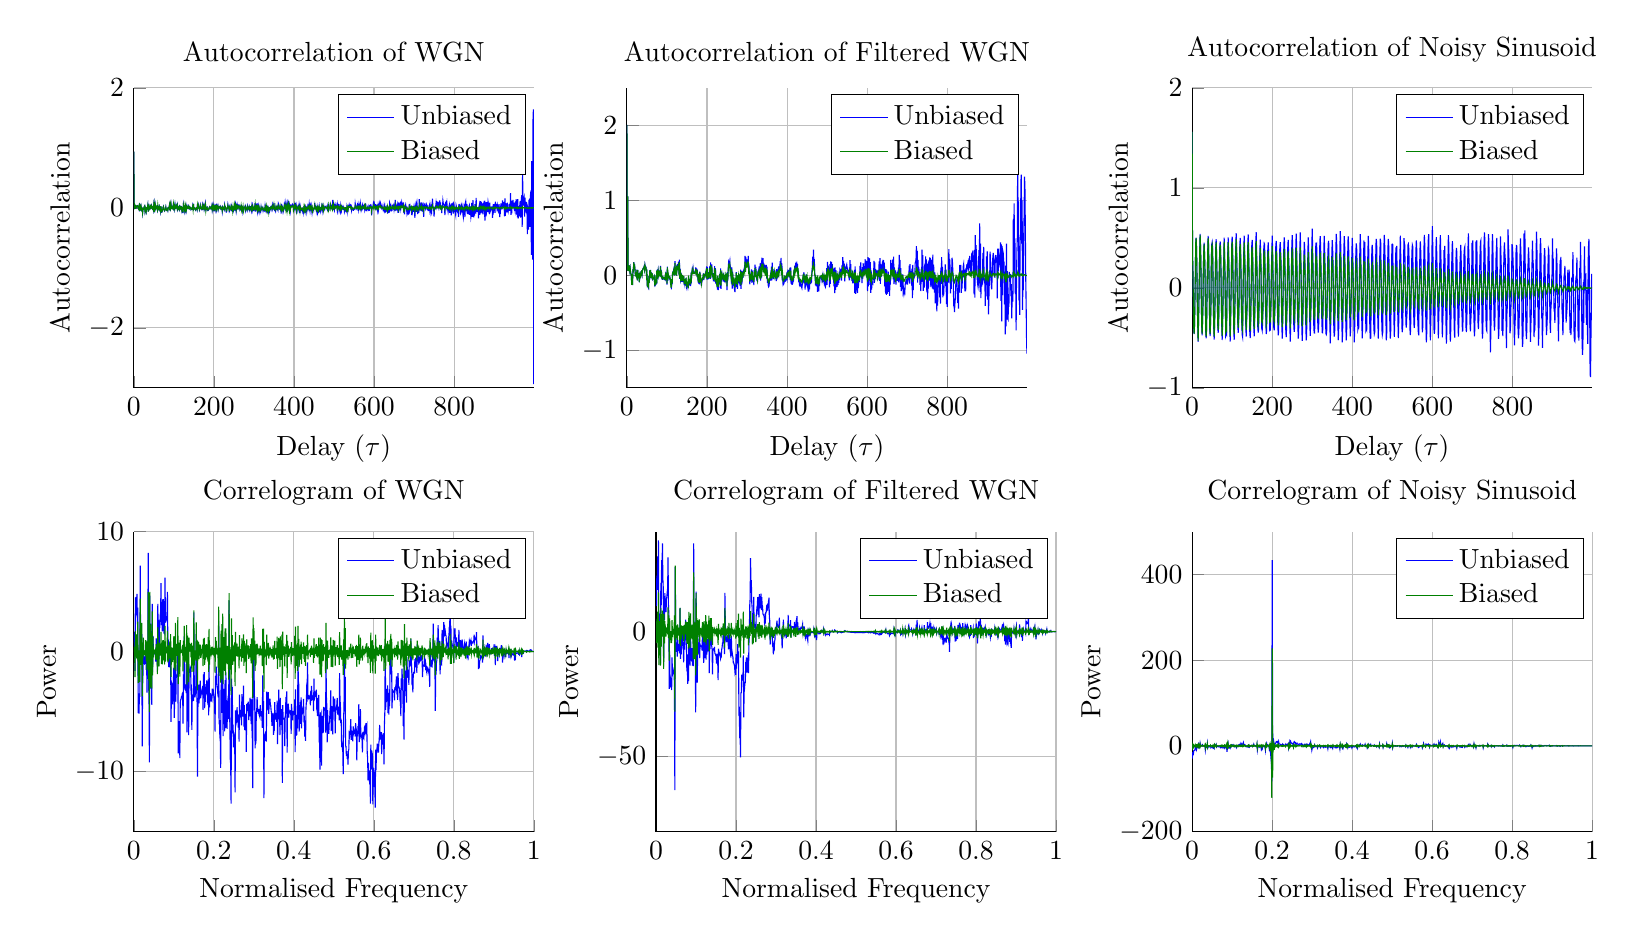
\begin{tikzpicture}

\begin{axis}[%
width=2in,
height=1.5in,
scale only axis,
xmin=0,
xmax=999,
xlabel={Delay ($\tau$)},
xmajorgrids,
ymin=-1.5,
ymax=2.5,
ylabel={Autocorrelation},
ymajorgrids,
name=plot3,
title={Autocorrelation of Filtered WGN},
axis x line*=bottom,
axis y line*=left,
legend style={draw=black,fill=white,legend cell align=left}
]
\addplot [color=blue,solid]
  table[row sep=crcr]{-999	-1.04363351459786\\
-998	-0.815393418274118\\
-997	-0.372948894421538\\
-996	-0.0103770255234643\\
-995	0.633423855500881\\
-994	1.18138138479025\\
-993	1.31502581509801\\
-992	0.815896416656528\\
-991	0.50363649253043\\
-990	-0.1953021425073\\
-989	-0.0623208969984734\\
-988	-0.460736844413034\\
-987	0.998697226826023\\
-986	0.422636304299663\\
-985	1.34394266846885\\
-984	1.25064180494122\\
-983	0.471963224087121\\
-982	0.510025065669935\\
-981	-0.525778308578391\\
-980	-0.203080960845305\\
-979	-0.33228967869119\\
-978	0.985319386508805\\
-977	0.581290893416081\\
-976	1.66264522154805\\
-975	0.50085929513947\\
-974	0.307686212046233\\
-973	-0.0524128016839269\\
-972	-0.732405975746396\\
-971	-0.0115030910098649\\
-970	-0.24900991326284\\
-969	0.493081953610079\\
-968	0.226574586899956\\
-967	0.958517276998491\\
-966	-0.00408138856109009\\
-965	0.753669296615314\\
-964	-0.348754301732965\\
-963	-0.205634581251323\\
-962	-0.326251373594918\\
-961	-0.574526521226671\\
-960	-0.117044334448687\\
-959	-0.276548538634285\\
-958	0.0132107040710342\\
-957	0.0130315032406713\\
-956	-0.0629114071239153\\
-955	0.0450849996345127\\
-954	-0.420282775980449\\
-953	-0.296492803302761\\
-952	-0.586472068895221\\
-951	-0.572449948068382\\
-950	0.057994671830281\\
-949	-0.589511655379882\\
-948	0.422506353218865\\
-947	-0.679105865398074\\
-946	0.13157833960864\\
-945	-0.785058994076771\\
-944	-0.095677851557563\\
-943	-0.3854161812548\\
-942	0.183950967371892\\
-941	0.137404060102939\\
-940	0.292227883752924\\
-939	0.31889582779064\\
-938	-0.262435176262816\\
-937	0.392937255991479\\
-936	-0.614163234633886\\
-935	0.412225226956488\\
-934	-0.339027290280635\\
-933	0.440815022040499\\
-932	0.102191742856405\\
-931	0.257516590021732\\
-930	0.201580682354975\\
-929	0.249374271159448\\
-928	0.357681880094559\\
-927	-0.0413467081156917\\
-926	0.355141967192458\\
-925	-0.307484370266039\\
-924	0.211177920410408\\
-923	0.172205980952393\\
-922	0.261217689458267\\
-921	0.263490775310009\\
-920	0.22390353455266\\
-919	-0.0327427805797715\\
-918	0.146858178152754\\
-917	0.0079437941785853\\
-916	0.212473584610194\\
-915	0.30039436898326\\
-914	0.251897835431449\\
-913	0.15975861323346\\
-912	-0.0449466316445\\
-911	-0.185500590871252\\
-910	-0.125240385695526\\
-909	0.0456877622607144\\
-908	0.177983490036617\\
-907	0.317156630209034\\
-906	-0.0371063312242737\\
-905	-0.092319610455751\\
-904	-0.307961396721437\\
-903	-0.518773409531226\\
-902	-0.0171870496984345\\
-901	-0.324642296503618\\
-900	0.321383389843046\\
-899	-0.1192067080648\\
-898	0.254574416414328\\
-897	-0.279329981886411\\
-896	-0.0256723603242004\\
-895	-0.405839921390248\\
-894	-0.0713724712295286\\
-893	-0.0813020517777816\\
-892	-0.0241487171389569\\
-891	0.381225012972074\\
-890	-0.0658432971270982\\
-889	0.300655315995305\\
-888	-0.121576186865806\\
-887	-0.0444570191510686\\
-886	-0.149990101624881\\
-885	0.0137040348258051\\
-884	-0.303406686864369\\
-883	0.424617330212631\\
-882	-0.219304594336568\\
-881	0.693825505716365\\
-880	0.0205901001278357\\
-879	0.335322280441673\\
-878	-0.102553062357567\\
-877	-0.152332835562867\\
-876	-0.117086699383064\\
-875	-0.0569560046778872\\
-874	0.170256267500391\\
-873	0.23131034764546\\
-872	0.402118150028732\\
-871	0.0331217112508355\\
-870	0.536646027242848\\
-869	-0.295635425135905\\
-868	0.341406904761206\\
-867	-0.254773314069943\\
-866	0.143287555260027\\
-865	-0.00147375030623251\\
-864	0.33127313042529\\
-863	0.249837696651866\\
-862	0.294584376495875\\
-861	0.283434931967355\\
-860	0.00624673992309011\\
-859	0.183634006352344\\
-858	0.0494383351678206\\
-857	0.172647903677639\\
-856	0.258491307169996\\
-855	0.0955983638793474\\
-854	0.226542554870719\\
-853	0.0833989317349563\\
-852	0.100222213414149\\
-851	0.145531991221578\\
-850	0.109239087194665\\
-849	0.14840599310295\\
-848	0.0432763585593717\\
-847	0.101466582559405\\
-846	-0.211559887963582\\
-845	-0.0120646809861329\\
-844	-0.214318803056287\\
-843	0.0772259974317009\\
-842	0.0437693054274404\\
-841	0.152671739260591\\
-840	0.124608241503215\\
-839	0.00948851911921479\\
-838	0.0252171040317903\\
-837	-0.177454846203651\\
-836	0.033937028718229\\
-835	-0.232262963388992\\
-834	0.14027334323948\\
-833	-0.029622249415874\\
-832	0.0483804289319053\\
-831	0.138105385346666\\
-830	-0.231096164905846\\
-829	-0.0743089172998092\\
-828	-0.444053323752499\\
-827	-0.250146456594666\\
-826	-0.365629542441597\\
-825	-0.187843414031856\\
-824	-0.0673701605432181\\
-823	-0.111242759504802\\
-822	-0.0290010480693421\\
-821	-0.172590382563087\\
-820	-0.318929015615383\\
-819	-0.390499066968244\\
-818	-0.489679813569858\\
-817	-0.353886180149101\\
-816	-0.370035871161104\\
-815	-0.0463527205972571\\
-814	0.0582833610749022\\
-813	0.172497244191376\\
-812	0.234564717677152\\
-811	0.0310669819868522\\
-810	-0.180477684920314\\
-809	-0.0580214063798645\\
-808	-0.240071399826351\\
-807	0.117447497572302\\
-806	0.218417366353082\\
-805	0.076523803352465\\
-804	0.35094394361032\\
-803	-0.0958865754402188\\
-802	-0.0585500562977668\\
-801	-0.078398610115434\\
-800	-0.421101398841462\\
-799	-0.0132609843021174\\
-798	-0.382390283664452\\
-797	0.0749426582208418\\
-796	-0.143254242171506\\
-795	0.147483725739245\\
-794	-0.0180492488533522\\
-793	-0.0149761029714219\\
-792	-0.141020431713003\\
-791	-0.268650201805541\\
-790	-0.146198272820216\\
-789	-0.293765082486601\\
-788	0.113125798836355\\
-787	-0.0878365230152614\\
-786	0.242536756872175\\
-785	-0.114485994621044\\
-784	0.102026277035956\\
-783	-0.375826116090936\\
-782	-0.00367579998958882\\
-781	-0.292333941609832\\
-780	-0.0200398305861199\\
-779	-0.0283385794625464\\
-778	-0.161253387720019\\
-777	-0.0558773354942843\\
-776	-0.402172620434134\\
-775	-0.195589912574743\\
-774	-0.480913956973914\\
-773	-0.121267784905008\\
-772	-0.374135776218247\\
-771	0.00637252874262444\\
-770	-0.374466687436208\\
-769	0.038749117662984\\
-768	-0.228565516514098\\
-767	-0.0333370971798334\\
-766	0.141991074311816\\
-765	-0.187836469650783\\
-764	0.277451334599427\\
-763	-0.174911865409052\\
-762	0.206805602410896\\
-761	-0.134917247970532\\
-760	0.178515038100089\\
-759	-0.157026211917172\\
-758	0.234097828942306\\
-757	-0.0691135266025139\\
-756	0.240268737582321\\
-755	-0.0264369041136323\\
-754	0.200072163991382\\
-753	-0.176287774996041\\
-752	0.155373085425498\\
-751	-0.320162411891588\\
-750	0.133245897228892\\
-749	-0.224059379058487\\
-748	0.213389760397435\\
-747	-0.0380900918181716\\
-746	0.253245739775719\\
-745	-0.0560623352441627\\
-744	0.155570969763806\\
-743	-0.162503597890283\\
-742	-0.0787216909796325\\
-741	-0.0469478111583977\\
-740	-0.206954993393662\\
-739	0.271216704442819\\
-738	-0.0819594193359097\\
-737	0.344242894494683\\
-736	-0.0856256139386184\\
-735	0.0879268839787315\\
-734	-0.210961371219659\\
-733	-0.0177473140889584\\
-732	-0.126477682278954\\
-731	0.0374735012215548\\
-730	0.0370407404103204\\
-729	0.106206182251417\\
-728	0.00864028234365415\\
-727	0.207555669246918\\
-726	-0.0974251583841542\\
-725	0.325628164360817\\
-724	0.0228516263248094\\
-723	0.390098567303832\\
-722	0.209946947187263\\
-721	0.181345268743806\\
-720	0.16695028393122\\
-719	-0.00648665552367264\\
-718	-0.0207021068818253\\
-717	0.00872690397768966\\
-716	0.0204860689190695\\
-715	-0.197550050560712\\
-714	0.139607537083428\\
-713	-0.30163646375727\\
-712	0.0911807976146714\\
-711	-0.136913387449996\\
-710	0.0598423378403371\\
-709	0.0114854893821284\\
-708	-0.0408170777916935\\
-707	0.149209391943998\\
-706	-0.110600816859829\\
-705	0.128136207337175\\
-704	-0.0447001379616759\\
-703	-0.0522841348679916\\
-702	-0.0126829161535802\\
-701	-0.122302168636536\\
-700	-0.0781314611297213\\
-699	-0.0586582579803318\\
-698	-0.0914834919591911\\
-697	-0.0729295699411848\\
-696	-0.092864520283798\\
-695	-0.121392278076231\\
-694	-0.227891970976494\\
-693	-0.210542326741654\\
-692	-0.245116675991139\\
-691	-0.188237043357705\\
-690	-0.216799937506776\\
-689	0.0140796560761454\\
-688	-0.186373222547489\\
-687	-0.0156624059431485\\
-686	-0.00473456597227443\\
-685	-0.208611455267537\\
-684	0.0977567308822029\\
-683	-0.15369249794411\\
-682	0.204866107585294\\
-681	-0.0457028662890265\\
-680	0.274590907540447\\
-679	-0.0935624187146587\\
-678	0.10432796564248\\
-677	-0.0651961322350344\\
-676	-0.0550953145517517\\
-675	-0.0110845679624149\\
-674	-0.0741480737395337\\
-673	0.00283736572255142\\
-672	-0.124405166668704\\
-671	0.0664965165230686\\
-670	-0.0899474481134355\\
-669	0.00904619618192852\\
-668	0.105380538354988\\
-667	-0.117167622017734\\
-666	0.250074807238321\\
-665	-0.0545382332464592\\
-664	0.210141662147127\\
-663	0.0384639283777349\\
-662	0.0925723747814932\\
-661	0.163793917658382\\
-660	0.032381808683531\\
-659	0.206878341296832\\
-658	-0.121830446554498\\
-657	-8.60381649881022e-05\\
-656	-0.271964632195568\\
-655	-0.00506609072092226\\
-654	-0.218637376246984\\
-653	0.0488370933927217\\
-652	-0.165671248784754\\
-651	-0.025702930453761\\
-650	-0.246028779738641\\
-649	0.0655475122921821\\
-648	-0.258496070894086\\
-647	0.0831993038157478\\
-646	-0.241576542423754\\
-645	0.0379512999143089\\
-644	-0.147909197400734\\
-643	0.169895208946157\\
-642	0.0679665594755405\\
-641	0.204473931476011\\
-640	0.148879604444391\\
-639	0.113600288191362\\
-638	0.148179117128455\\
-637	0.0702547036639643\\
-636	0.143433067837113\\
-635	-0.0190608063487476\\
-634	0.15457107025356\\
-633	-0.111771210395885\\
-632	0.228837170618131\\
-631	-0.071743104126098\\
-630	0.185941545882583\\
-629	0.0625693460930249\\
-628	0.0221401040886883\\
-627	0.0734860655811582\\
-626	-0.0673862035969657\\
-625	0.030321833114157\\
-624	0.0148781716745851\\
-623	0.0581122958396529\\
-622	0.0677636611538852\\
-621	0.049266310903724\\
-620	-0.0491740462003995\\
-619	0.173371480197314\\
-618	-0.101369027815569\\
-617	0.193152314035515\\
-616	-0.0355538447051377\\
-615	0.00359136627491825\\
-614	-0.109795044103616\\
-613	-0.100003957854625\\
-612	-0.118882216919753\\
-611	-0.188005409665871\\
-610	0.0651930541312509\\
-609	-0.232591394773502\\
-608	0.177607965965497\\
-607	-0.125952332579827\\
-606	0.226188591157512\\
-605	-0.0355798242633409\\
-604	0.230948100458757\\
-603	-0.148209546819232\\
-602	0.243725819168297\\
-601	-0.211174168946405\\
-600	0.189681081389456\\
-599	-0.0262464555726736\\
-598	0.0506105299402483\\
-597	0.194886111419383\\
-596	0.0435117761796245\\
-595	0.215822635178714\\
-594	0.0398136471574751\\
-593	0.0878534833610025\\
-592	0.0556882664943471\\
-591	0.0289924480184822\\
-590	0.163380128558339\\
-589	-0.0443773849659172\\
-588	0.108322830511996\\
-587	-0.104655697315082\\
-586	0.0731928479852909\\
-585	-0.0281463704386725\\
-584	0.172214594530663\\
-583	-0.0174309930635532\\
-582	0.126792345416806\\
-581	-0.0886010596602731\\
-580	-0.032008082296915\\
-579	-0.0283116362222452\\
-578	-0.168913808401335\\
-577	-0.0207419872232183\\
-576	-0.232285906769134\\
-575	-0.0821976997359977\\
-574	-0.171605136450106\\
-573	-0.134921041093445\\
-572	-0.015649557583459\\
-571	-0.246743209832358\\
-570	0.118842037607456\\
-569	-0.234531534224594\\
-568	0.0731062307869774\\
-567	-0.103291804073402\\
-566	-0.0470447722605344\\
-565	0.0172934754464709\\
-564	-0.106255587636175\\
-563	0.0279199426013876\\
-562	-0.0713382939923114\\
-561	0.00774918754642565\\
-560	0.00419334899963453\\
-559	0.150889270078587\\
-558	-0.0310635551654649\\
-557	0.204680402951894\\
-556	-0.0671215253862196\\
-555	0.0726454557985221\\
-554	-0.00617432910267686\\
-553	0.0307176278416534\\
-552	0.0520715671115544\\
-551	0.0947721568429137\\
-550	0.0936890069886494\\
-549	0.144627469641633\\
-548	0.127669914488629\\
-547	0.094894396893292\\
-546	0.039238881837479\\
-545	0.116280187207565\\
-544	-0.0783404716858793\\
-543	0.155265918350937\\
-542	0.0275090814999468\\
-541	0.192993379171168\\
-540	0.132375803666385\\
-539	0.243682212652897\\
-538	0.0242780100519294\\
-537	0.133109040167858\\
-536	-0.0706475678332248\\
-535	0.0883980458062734\\
-534	-0.00742920311421823\\
-533	0.0470888301811684\\
-532	0.0660012241868136\\
-531	-0.0636814869732107\\
-530	0.0502705871189139\\
-529	-0.100183221263006\\
-528	0.0035955406519815\\
-527	-0.129881440332815\\
-526	-0.0279191087412514\\
-525	-0.152248751501673\\
-524	0.0134654277334169\\
-523	-0.157377144267124\\
-522	0.0714532677784389\\
-521	-0.191554709460392\\
-520	0.105556347326613\\
-519	-0.238125986381746\\
-518	0.100457152242553\\
-517	-0.146127420049394\\
-516	0.00670332097091019\\
-515	0.0492814353566478\\
-514	-0.0061836006202535\\
-513	0.150320374889297\\
-512	0.0694512038880981\\
-511	0.176100397479238\\
-510	0.0471274099684376\\
-509	0.186669921360365\\
-508	-0.112304020208373\\
-507	0.148903114847071\\
-506	-0.16041310530124\\
-505	0.107584575355066\\
-504	0.0405497923755594\\
-503	0.129635083685404\\
-502	0.0422386447405541\\
-501	0.179422271239003\\
-500	-0.127234847436161\\
-499	0.0966428207434955\\
-498	-0.0867029521006854\\
-497	-0.115185498669592\\
-496	-0.056151515511808\\
-495	-0.143885978970001\\
-494	-0.127295880880691\\
-493	-0.0250558658864456\\
-492	-0.0728947600448959\\
-491	-0.0300826228508302\\
-490	0.00163415116640336\\
-489	-0.0889010452957629\\
-488	-0.0174997416213614\\
-487	-0.0680713145499883\\
-486	-0.0353847389491655\\
-485	-0.0126716602442486\\
-484	-0.0245235424952779\\
-483	-0.0292520427707615\\
-482	-0.0509104305956739\\
-481	-0.136204886977032\\
-480	-0.0903926493319941\\
-479	-0.213470393871124\\
-478	-0.178789124219512\\
-477	-0.123477290374779\\
-476	-0.220143919503695\\
-475	-0.0629526679797923\\
-474	-0.0934886825771027\\
-473	-0.145595438888114\\
-472	-0.0752171760732223\\
-471	-0.132342925812069\\
-470	-0.0172877532127258\\
-469	0.0256066714734926\\
-468	0.21640426281275\\
-467	0.120712407427533\\
-466	0.341517043401084\\
-465	0.167672531379741\\
-464	0.244823898291092\\
-463	0.10155791652107\\
-462	0.047508399989672\\
-461	-0.0742979407713487\\
-460	-0.0570849738965563\\
-459	-0.0578257594754937\\
-458	-0.115826520292563\\
-457	-0.0333210584573663\\
-456	-0.187375297574722\\
-455	-0.0967052409045339\\
-454	-0.217607619709352\\
-453	-0.134940335813021\\
-452	-0.172133177769243\\
-451	-0.131042341341243\\
-450	-0.0283511531102268\\
-449	-0.0913281903057196\\
-448	0.0142053686157023\\
-447	-0.149339303380931\\
-446	-0.0633782297487008\\
-445	-0.191115153412443\\
-444	-0.0176901680547446\\
-443	-0.107111469237644\\
-442	0.0429177541482039\\
-441	-0.0293783187094339\\
-440	-0.0170237647131021\\
-439	-0.0921448344607363\\
-438	-0.11886108410245\\
-437	-0.168382219300048\\
-436	-0.150510107770763\\
-435	-0.138615341771446\\
-434	-0.10661100697887\\
-433	-0.12589942294672\\
-432	-0.108074865242562\\
-431	-0.123677800333416\\
-430	-0.0642499109046386\\
-429	-0.0706556124967429\\
-428	0.0638788390605739\\
-427	0.0126450091327192\\
-426	0.153590076265782\\
-425	0.120465031292617\\
-424	0.165845025405849\\
-423	0.154135470411936\\
-422	0.10759339469779\\
-421	0.13118146418264\\
-420	0.0642091599352602\\
-419	0.125890440525358\\
-418	0.0246690048477848\\
-417	0.0654600258676778\\
-416	-0.0564632835535846\\
-415	-0.0435797302440827\\
-414	-0.107663760829703\\
-413	-0.118745150866733\\
-412	-0.118902404796852\\
-411	-0.013239148280661\\
-410	-0.112115302963194\\
-409	0.107400818164292\\
-408	-0.0646727661451931\\
-407	0.103365831244846\\
-406	-0.0259997798803164\\
-405	0.0697912034263317\\
-404	0.0131424735486226\\
-403	0.0383083883469368\\
-402	0.00880008940820691\\
-401	0.0323302064190248\\
-400	-0.0381255330871025\\
-399	-0.00432061429014373\\
-398	-0.0534096481340085\\
-397	-0.064326403355663\\
-396	-0.0379032784611924\\
-395	-0.0604426605046968\\
-394	-0.036054627622287\\
-393	-0.0734737080474841\\
-392	-0.111534041969672\\
-391	-0.118891974961638\\
-390	-0.127390861041465\\
-389	-0.00158308833206266\\
-388	-0.0648594139006499\\
-387	0.160826874425125\\
-386	0.00647014323847761\\
-385	0.231547805976654\\
-384	0.0971626283293954\\
-383	0.190927932834994\\
-382	0.123140259012826\\
-381	0.102238882360649\\
-380	0.0389494338830141\\
-379	0.12061822174384\\
-378	-0.0275679094277413\\
-377	0.0646579639192797\\
-376	0.0410342723513924\\
-375	-0.0532203121776232\\
-374	0.0826813800884705\\
-373	-0.0763447498504959\\
-372	0.00258614282820339\\
-371	-0.0266253962093189\\
-370	-0.0105251643719949\\
-369	0.0681095622277292\\
-368	-0.00781540909134312\\
-367	0.060030049936706\\
-366	-0.0509930966273133\\
-365	0.0874727129140728\\
-364	-0.036577316270435\\
-363	0.170687188426994\\
-362	-0.0667969942512456\\
-361	0.115654343536955\\
-360	-0.069303282763808\\
-359	0.0177102297398312\\
-358	-0.015350256527936\\
-357	-0.064247947876866\\
-356	-0.0696154584440945\\
-355	-0.13969120741591\\
-354	-0.15204287107578\\
-353	-0.135022697029114\\
-352	-0.0727257180939212\\
-351	-0.0798738899972572\\
-350	0.115908763325047\\
-349	-0.0445151829179148\\
-348	0.140788513419813\\
-347	-0.0024876413581307\\
-346	0.106020902364141\\
-345	0.0593171179784411\\
-344	0.141388397979843\\
-343	0.0392165041205666\\
-342	0.159651872668595\\
-341	0.0687321432858777\\
-340	0.221240200238566\\
-339	0.219687109941465\\
-338	0.154893265716913\\
-337	0.236539852337069\\
-336	-0.0304188311506921\\
-335	0.167966383672038\\
-334	-0.070445117570371\\
-333	0.160953255902271\\
-332	-0.0404801848410547\\
-331	0.120042137769742\\
-330	0.016182409844642\\
-329	0.0636467151406772\\
-328	0.0282520173730935\\
-327	0.03832603246326\\
-326	-0.0862089700537686\\
-325	-0.0292820789080909\\
-324	-0.0448923940621195\\
-323	-0.0146183721958273\\
-322	0.112084830750243\\
-321	0.0509774553601651\\
-320	0.14220598570714\\
-319	-0.0198259477881476\\
-318	0.0686351195552827\\
-317	-0.130537334645821\\
-316	-0.0154449478465503\\
-315	-0.0824882458604439\\
-314	-0.080461772359904\\
-313	0.0636744456243459\\
-312	-0.0985175595282143\\
-311	0.0800988542483286\\
-310	-0.00196911543268269\\
-309	-0.0722073961978562\\
-308	0.0213606589796812\\
-307	-0.120773953299136\\
-306	-0.0135315568201781\\
-305	0.10100674905661\\
-304	0.0767774668646748\\
-303	0.260661785255525\\
-302	0.151230214653581\\
-301	0.212221497254165\\
-300	0.164263474528681\\
-299	0.158964718803385\\
-298	0.153748681966071\\
-297	0.246668414121229\\
-296	0.0643604451622279\\
-295	0.259847761649349\\
-294	0.0531707636326976\\
-293	0.0909537044457016\\
-292	0.069917998126588\\
-291	0.0660696060715637\\
-290	-0.0332206317883896\\
-289	0.0535083502060757\\
-288	-0.0416229968921667\\
-287	-0.118635386956455\\
-286	0.0601460079488946\\
-285	-0.179659644849917\\
-284	0.077317205369157\\
-283	-0.140559880783286\\
-282	0.0133306433398583\\
-281	-0.0803215709857943\\
-280	-0.0480159008266721\\
-279	-0.00151892940739528\\
-278	-0.107871486889191\\
-277	-0.0164839876419328\\
-276	-0.179333334665256\\
-275	0.00279112899516333\\
-274	-0.157187999417667\\
-273	0.0436488492288501\\
-272	-0.148494176083181\\
-271	-0.0448382709079089\\
-270	-0.221449166380465\\
-269	-0.118367772513843\\
-268	-0.161588230024726\\
-267	-0.125958471390317\\
-266	-0.0387622149445972\\
-265	-0.135809125908628\\
-264	0.0498714918567412\\
-263	-0.177774206914042\\
-262	0.106417075931887\\
-261	-0.111283953049953\\
-260	0.0759331090307746\\
-259	0.101198733213534\\
-258	0.0561375712075762\\
-257	0.190198323853867\\
-256	0.158702636037994\\
-255	0.1511095136889\\
-254	0.172809140795804\\
-253	0.085290472378727\\
-252	-0.0701648570998585\\
-251	0.0418230943048738\\
-250	-0.196117952376165\\
-249	0.0253677380149616\\
-248	-0.0926133747172275\\
-247	-0.0126216271278218\\
-246	-0.0715849705749812\\
-245	-0.0214854727062282\\
-244	-0.0912737302018361\\
-243	0.00469032026600658\\
-242	-0.0815132075866314\\
-241	-0.0105523925549729\\
-240	-0.0411700375148754\\
-239	-0.0259098541537948\\
-238	0.0135285929071386\\
-237	-0.0824425105392952\\
-236	0.0521541478757303\\
-235	-0.178770222622829\\
-234	0.0923338472220928\\
-233	-0.167097685326355\\
-232	0.0217581211784663\\
-231	-0.110792961517042\\
-230	-0.107166417290001\\
-229	-0.0463748961886978\\
-228	-0.197690327305036\\
-227	-0.00580711873661304\\
-226	-0.189387027095872\\
-225	-0.0722344603964152\\
-224	-0.128861137474299\\
-223	-0.063293237646316\\
-222	-0.110567220392975\\
-221	0.0980566579837259\\
-220	-0.0854730391526121\\
-219	0.122133496182033\\
-218	-0.0597220420317676\\
-217	0.0301339755442529\\
-216	-0.0796079903216469\\
-215	0.0201057094653965\\
-214	0.0238467617957407\\
-213	0.00545158010135406\\
-212	0.147431759049758\\
-211	0.0595882391177864\\
-210	0.0364536245933713\\
-209	0.171778553948424\\
-208	-0.0464304595278989\\
-207	0.11967158738872\\
-206	-0.0281805750605865\\
-205	0.0319724419094905\\
-204	-0.0449509351578904\\
-203	0.0435120542819007\\
-202	-0.0547011488250916\\
-201	0.112009185426442\\
-200	-0.0578887337452099\\
-199	0.118634361361266\\
-198	-0.0323338747407007\\
-197	0.0461047794766446\\
-196	0.0234936763588192\\
-195	-0.0024893389411989\\
-194	-0.0066373103310587\\
-193	0.0045798650805042\\
-192	-0.0641853224242818\\
-191	0.0269401134670081\\
-190	-0.031028104614798\\
-189	-0.0360675267936719\\
-188	-0.0672392408780297\\
-187	-0.0832885859503791\\
-186	-0.138491927353381\\
-185	-0.0755711411492776\\
-184	-0.0338089362921981\\
-183	-0.103437554271849\\
-182	0.0481611754166706\\
-181	-0.120468818504238\\
-180	0.0151525985588763\\
-179	-0.11124521064539\\
-178	0.019722165199779\\
-177	-0.0232308897563331\\
-176	0.0418255805108938\\
-175	0.0203178661061408\\
-174	0.0938971999915839\\
-173	0.00292757335583014\\
-172	0.105077163303892\\
-171	0.0471057252447578\\
-170	0.0528566810805744\\
-169	0.0285889307866693\\
-168	0.0294752468004741\\
-167	0.0319765622127797\\
-166	0.0290663616135366\\
-165	0.0939739411313917\\
-164	0.0544023059418741\\
-163	0.0765088286581258\\
-162	0.0364836653103949\\
-161	-0.0552602958102783\\
-160	-0.0248333235644841\\
-159	-0.143430778485294\\
-158	-0.0718595856711487\\
-157	-0.0823257068423137\\
-156	-0.103059728085714\\
-155	-0.0650022689935252\\
-154	-0.13389524081638\\
-153	-0.0771235295366499\\
-152	-0.147067034724923\\
-151	-0.113606520323097\\
-150	-0.108550013120893\\
-149	-0.143835774279284\\
-148	-0.0754631179280989\\
-147	-0.101366977307711\\
-146	-0.0778057254512771\\
-145	-0.115431886144741\\
-144	-0.0552222883709299\\
-143	-0.130217511960649\\
-142	-0.0138501063056188\\
-141	-0.0917683019186468\\
-140	-0.00626147718878808\\
-139	-0.0873389420846605\\
-138	0.00640534486627103\\
-137	-0.0868474479362875\\
-136	-0.00873342995839129\\
-135	-0.033943440857821\\
-134	-0.0581354010230789\\
-133	0.0882067769075481\\
-132	-0.0477665454515415\\
-131	0.208257251421964\\
-130	0.0109958762991628\\
-129	0.183877048612003\\
-128	0.0764900401932535\\
-127	0.14911905717787\\
-126	0.0799082646137254\\
-125	0.143225953097721\\
-124	-0.00306740049477434\\
-123	0.0819796937873217\\
-122	0.042303843006832\\
-121	0.0306020517950055\\
-120	0.188112323654164\\
-119	0.000491797362104517\\
-118	0.120680116955786\\
-117	0.0372868653975865\\
-116	0.0537232473505195\\
-115	0.0247264234742079\\
-114	0.0322244516511055\\
-113	-0.119441428084153\\
-112	-0.0626577241969367\\
-111	-0.18499223864241\\
-110	-0.0576195886550194\\
-109	-0.107217736719664\\
-108	-0.0440292816790989\\
-107	-0.0249740161598221\\
-106	-0.0378075579981581\\
-105	-0.0246501878996028\\
-104	-0.0170044466596933\\
-103	0.0250666246271362\\
-102	-0.0718331673545915\\
-101	0.117028131073322\\
-100	-0.121770699533439\\
-99	0.0359882396672716\\
-98	-0.0584451656621185\\
-97	-0.0585311616163053\\
-96	-0.00826453347747701\\
-95	-0.0568612477038494\\
-94	-0.046609859370896\\
-93	-0.0503741324734114\\
-92	-0.0314453217338547\\
-91	-0.0332994560380093\\
-90	-0.024674500472136\\
-89	-0.0516410677393995\\
-88	-0.0508088195473588\\
-87	-0.0291294527926572\\
-86	0.0661595703189276\\
-85	-0.0022984589175748\\
-84	0.125869901652185\\
-83	-0.024465646307259\\
-82	0.0661878124034748\\
-81	-0.00562567064121403\\
-80	0.0663277297850711\\
-79	0.0134320884262418\\
-78	0.0665838441640203\\
-77	0.02058408591205\\
-76	0.0791526956539579\\
-75	-0.0387718960884523\\
-74	-0.00500454778880552\\
-73	-0.115519466188512\\
-72	-0.113623660517647\\
-71	-0.126208744628982\\
-70	-0.0586826610126015\\
-69	-0.0932039257278569\\
-68	-0.0218700405570183\\
-67	-0.0409339626178173\\
-66	-0.039348645061776\\
-65	-0.0481170765091857\\
-64	-0.00958346909664462\\
-63	-0.0379121192130143\\
-62	-0.0179159292304408\\
-61	0.0400557428651967\\
-60	-0.0352338151067965\\
-59	0.0735049343983383\\
-58	-0.0319636532207356\\
-57	0.065834615365273\\
-56	-0.10111194965723\\
-55	-0.00932092777047381\\
-54	-0.167335306191132\\
-53	-0.154605849592684\\
-52	-0.107908239614522\\
-51	-0.158593405730717\\
-50	0.0198795846641712\\
-49	-0.00669527020813078\\
-48	0.100853524307399\\
-47	0.113375514245935\\
-46	0.10260692679183\\
-45	0.137314550993774\\
-44	0.0803584517200142\\
-43	0.120449254235359\\
-42	0.103115446368568\\
-41	0.0977726203009288\\
-40	0.0894314602829086\\
-39	0.0702031737770385\\
-38	0.0200883735018632\\
-37	0.0674375821194236\\
-36	-0.00594482382568309\\
-35	0.0533452998150266\\
-34	-0.0186781858071727\\
-33	-0.0305556730616651\\
-32	-0.00447875522991109\\
-31	-0.0916551204950295\\
-30	0.0280178276826789\\
-29	-0.027686208994281\\
-28	-0.0308236488308933\\
-27	0.0721394981482458\\
-26	-0.0665723451240716\\
-25	0.0757438182345833\\
-24	-0.0225229856209991\\
-23	-0.0107877327601332\\
-22	0.0225830790277231\\
-21	0.012250207050634\\
-20	0.0862469520584132\\
-19	0.139093627995982\\
-18	0.138059157858124\\
-17	0.174969623639052\\
-16	0.0419740612965344\\
-15	0.0812454923263921\\
-14	-0.129276662658293\\
-13	0.00277898977593677\\
-12	-0.126548363012727\\
-11	0.0123613463482388\\
-10	0.015055381201447\\
-9	0.0463455973248565\\
-8	0.0983231304904412\\
-7	0.0671684330870433\\
-6	0.13261775947866\\
-5	0.0588308503002559\\
-4	0.134854102151819\\
-3	0.0611154265071904\\
-2	1.05481719408915\\
-1	0.0650618432594144\\
0	2.00756555636676\\
1	0.0650618432594143\\
2	1.05481719408915\\
3	0.0611154265071904\\
4	0.134854102151819\\
5	0.0588308503002559\\
6	0.13261775947866\\
7	0.0671684330870433\\
8	0.0983231304904412\\
9	0.0463455973248565\\
10	0.015055381201447\\
11	0.0123613463482388\\
12	-0.126548363012727\\
13	0.00277898977593676\\
14	-0.129276662658293\\
15	0.0812454923263921\\
16	0.0419740612965344\\
17	0.174969623639052\\
18	0.138059157858124\\
19	0.139093627995982\\
20	0.0862469520584132\\
21	0.012250207050634\\
22	0.0225830790277231\\
23	-0.0107877327601332\\
24	-0.0225229856209991\\
25	0.0757438182345833\\
26	-0.0665723451240715\\
27	0.0721394981482458\\
28	-0.0308236488308933\\
29	-0.027686208994281\\
30	0.0280178276826789\\
31	-0.0916551204950295\\
32	-0.00447875522991109\\
33	-0.0305556730616651\\
34	-0.0186781858071727\\
35	0.0533452998150266\\
36	-0.00594482382568306\\
37	0.0674375821194236\\
38	0.0200883735018632\\
39	0.0702031737770385\\
40	0.0894314602829086\\
41	0.0977726203009289\\
42	0.103115446368568\\
43	0.120449254235359\\
44	0.0803584517200142\\
45	0.137314550993774\\
46	0.10260692679183\\
47	0.113375514245935\\
48	0.100853524307399\\
49	-0.0066952702081308\\
50	0.0198795846641712\\
51	-0.158593405730717\\
52	-0.107908239614522\\
53	-0.154605849592684\\
54	-0.167335306191132\\
55	-0.00932092777047379\\
56	-0.10111194965723\\
57	0.065834615365273\\
58	-0.0319636532207355\\
59	0.0735049343983383\\
60	-0.0352338151067964\\
61	0.0400557428651967\\
62	-0.0179159292304408\\
63	-0.0379121192130143\\
64	-0.00958346909664462\\
65	-0.0481170765091857\\
66	-0.039348645061776\\
67	-0.0409339626178174\\
68	-0.0218700405570183\\
69	-0.0932039257278569\\
70	-0.0586826610126015\\
71	-0.126208744628982\\
72	-0.113623660517647\\
73	-0.115519466188512\\
74	-0.00500454778880554\\
75	-0.0387718960884523\\
76	0.0791526956539579\\
77	0.02058408591205\\
78	0.0665838441640203\\
79	0.0134320884262418\\
80	0.0663277297850711\\
81	-0.00562567064121403\\
82	0.0661878124034748\\
83	-0.024465646307259\\
84	0.125869901652185\\
85	-0.00229845891757478\\
86	0.0661595703189277\\
87	-0.0291294527926572\\
88	-0.0508088195473588\\
89	-0.0516410677393995\\
90	-0.024674500472136\\
91	-0.0332994560380093\\
92	-0.0314453217338547\\
93	-0.0503741324734114\\
94	-0.046609859370896\\
95	-0.0568612477038494\\
96	-0.00826453347747701\\
97	-0.0585311616163053\\
98	-0.0584451656621185\\
99	0.0359882396672716\\
100	-0.121770699533439\\
101	0.117028131073322\\
102	-0.0718331673545915\\
103	0.0250666246271362\\
104	-0.0170044466596934\\
105	-0.0246501878996028\\
106	-0.0378075579981581\\
107	-0.0249740161598221\\
108	-0.0440292816790989\\
109	-0.107217736719664\\
110	-0.0576195886550194\\
111	-0.18499223864241\\
112	-0.0626577241969367\\
113	-0.119441428084153\\
114	0.0322244516511055\\
115	0.0247264234742079\\
116	0.0537232473505195\\
117	0.0372868653975865\\
118	0.120680116955786\\
119	0.000491797362104533\\
120	0.188112323654164\\
121	0.0306020517950055\\
122	0.042303843006832\\
123	0.0819796937873216\\
124	-0.00306740049477436\\
125	0.143225953097721\\
126	0.0799082646137254\\
127	0.14911905717787\\
128	0.0764900401932535\\
129	0.183877048612003\\
130	0.0109958762991628\\
131	0.208257251421964\\
132	-0.0477665454515415\\
133	0.0882067769075481\\
134	-0.0581354010230789\\
135	-0.0339434408578209\\
136	-0.00873342995839129\\
137	-0.0868474479362874\\
138	0.00640534486627101\\
139	-0.0873389420846605\\
140	-0.00626147718878808\\
141	-0.0917683019186468\\
142	-0.0138501063056188\\
143	-0.130217511960649\\
144	-0.0552222883709299\\
145	-0.115431886144741\\
146	-0.0778057254512772\\
147	-0.101366977307711\\
148	-0.0754631179280989\\
149	-0.143835774279284\\
150	-0.108550013120893\\
151	-0.113606520323097\\
152	-0.147067034724923\\
153	-0.0771235295366499\\
154	-0.13389524081638\\
155	-0.0650022689935252\\
156	-0.103059728085714\\
157	-0.0823257068423137\\
158	-0.0718595856711487\\
159	-0.143430778485294\\
160	-0.0248333235644841\\
161	-0.0552602958102783\\
162	0.0364836653103949\\
163	0.0765088286581258\\
164	0.0544023059418741\\
165	0.0939739411313917\\
166	0.0290663616135366\\
167	0.0319765622127797\\
168	0.0294752468004741\\
169	0.0285889307866693\\
170	0.0528566810805744\\
171	0.0471057252447578\\
172	0.105077163303892\\
173	0.00292757335583012\\
174	0.0938971999915839\\
175	0.0203178661061408\\
176	0.0418255805108938\\
177	-0.0232308897563332\\
178	0.0197221651997789\\
179	-0.11124521064539\\
180	0.0151525985588763\\
181	-0.120468818504238\\
182	0.0481611754166706\\
183	-0.103437554271849\\
184	-0.0338089362921981\\
185	-0.0755711411492776\\
186	-0.13849192735338\\
187	-0.0832885859503791\\
188	-0.0672392408780297\\
189	-0.0360675267936719\\
190	-0.031028104614798\\
191	0.0269401134670081\\
192	-0.0641853224242818\\
193	0.0045798650805042\\
194	-0.00663731033105864\\
195	-0.00248933894119889\\
196	0.0234936763588192\\
197	0.0461047794766446\\
198	-0.0323338747407007\\
199	0.118634361361266\\
200	-0.0578887337452099\\
201	0.112009185426442\\
202	-0.0547011488250916\\
203	0.0435120542819007\\
204	-0.0449509351578903\\
205	0.0319724419094905\\
206	-0.0281805750605865\\
207	0.11967158738872\\
208	-0.0464304595278989\\
209	0.171778553948424\\
210	0.0364536245933713\\
211	0.0595882391177864\\
212	0.147431759049758\\
213	0.00545158010135405\\
214	0.0238467617957407\\
215	0.0201057094653965\\
216	-0.0796079903216469\\
217	0.0301339755442529\\
218	-0.0597220420317676\\
219	0.122133496182033\\
220	-0.0854730391526121\\
221	0.0980566579837259\\
222	-0.110567220392975\\
223	-0.063293237646316\\
224	-0.128861137474299\\
225	-0.0722344603964152\\
226	-0.189387027095872\\
227	-0.00580711873661305\\
228	-0.197690327305036\\
229	-0.0463748961886978\\
230	-0.107166417290001\\
231	-0.110792961517042\\
232	0.0217581211784663\\
233	-0.167097685326355\\
234	0.0923338472220928\\
235	-0.178770222622829\\
236	0.0521541478757303\\
237	-0.0824425105392952\\
238	0.0135285929071386\\
239	-0.0259098541537949\\
240	-0.0411700375148754\\
241	-0.0105523925549729\\
242	-0.0815132075866314\\
243	0.0046903202660066\\
244	-0.0912737302018361\\
245	-0.0214854727062282\\
246	-0.0715849705749812\\
247	-0.0126216271278218\\
248	-0.0926133747172276\\
249	0.0253677380149617\\
250	-0.196117952376165\\
251	0.0418230943048738\\
252	-0.0701648570998586\\
253	0.085290472378727\\
254	0.172809140795804\\
255	0.1511095136889\\
256	0.158702636037994\\
257	0.190198323853867\\
258	0.0561375712075762\\
259	0.101198733213534\\
260	0.0759331090307746\\
261	-0.111283953049953\\
262	0.106417075931887\\
263	-0.177774206914042\\
264	0.0498714918567412\\
265	-0.135809125908628\\
266	-0.0387622149445972\\
267	-0.125958471390317\\
268	-0.161588230024726\\
269	-0.118367772513843\\
270	-0.221449166380465\\
271	-0.0448382709079088\\
272	-0.148494176083181\\
273	0.0436488492288501\\
274	-0.157187999417667\\
275	0.00279112899516329\\
276	-0.179333334665256\\
277	-0.0164839876419327\\
278	-0.107871486889191\\
279	-0.0015189294073953\\
280	-0.0480159008266721\\
281	-0.0803215709857942\\
282	0.0133306433398582\\
283	-0.140559880783286\\
284	0.077317205369157\\
285	-0.179659644849917\\
286	0.0601460079488946\\
287	-0.118635386956455\\
288	-0.0416229968921667\\
289	0.0535083502060757\\
290	-0.0332206317883895\\
291	0.0660696060715637\\
292	0.069917998126588\\
293	0.0909537044457017\\
294	0.0531707636326976\\
295	0.259847761649349\\
296	0.0643604451622279\\
297	0.246668414121229\\
298	0.153748681966071\\
299	0.158964718803385\\
300	0.164263474528681\\
301	0.212221497254165\\
302	0.151230214653581\\
303	0.260661785255525\\
304	0.0767774668646747\\
305	0.10100674905661\\
306	-0.0135315568201782\\
307	-0.120773953299136\\
308	0.0213606589796812\\
309	-0.0722073961978562\\
310	-0.0019691154326827\\
311	0.0800988542483286\\
312	-0.0985175595282143\\
313	0.0636744456243458\\
314	-0.080461772359904\\
315	-0.0824882458604439\\
316	-0.0154449478465502\\
317	-0.130537334645821\\
318	0.0686351195552827\\
319	-0.0198259477881476\\
320	0.14220598570714\\
321	0.050977455360165\\
322	0.112084830750243\\
323	-0.0146183721958273\\
324	-0.0448923940621194\\
325	-0.0292820789080909\\
326	-0.0862089700537686\\
327	0.0383260324632599\\
328	0.0282520173730935\\
329	0.0636467151406771\\
330	0.016182409844642\\
331	0.120042137769742\\
332	-0.0404801848410548\\
333	0.160953255902271\\
334	-0.0704451175703711\\
335	0.167966383672038\\
336	-0.0304188311506921\\
337	0.236539852337069\\
338	0.154893265716913\\
339	0.219687109941465\\
340	0.221240200238566\\
341	0.0687321432858777\\
342	0.159651872668595\\
343	0.0392165041205667\\
344	0.141388397979843\\
345	0.0593171179784412\\
346	0.106020902364141\\
347	-0.00248764135813072\\
348	0.140788513419813\\
349	-0.0445151829179148\\
350	0.115908763325047\\
351	-0.0798738899972572\\
352	-0.0727257180939212\\
353	-0.135022697029114\\
354	-0.15204287107578\\
355	-0.13969120741591\\
356	-0.0696154584440945\\
357	-0.064247947876866\\
358	-0.015350256527936\\
359	0.0177102297398312\\
360	-0.069303282763808\\
361	0.115654343536955\\
362	-0.0667969942512456\\
363	0.170687188426994\\
364	-0.036577316270435\\
365	0.0874727129140728\\
366	-0.0509930966273133\\
367	0.060030049936706\\
368	-0.0078154090913431\\
369	0.0681095622277292\\
370	-0.0105251643719949\\
371	-0.0266253962093189\\
372	0.00258614282820343\\
373	-0.0763447498504959\\
374	0.0826813800884704\\
375	-0.0532203121776232\\
376	0.0410342723513925\\
377	0.0646579639192798\\
378	-0.0275679094277413\\
379	0.12061822174384\\
380	0.0389494338830141\\
381	0.102238882360649\\
382	0.123140259012826\\
383	0.190927932834994\\
384	0.0971626283293954\\
385	0.231547805976654\\
386	0.00647014323847754\\
387	0.160826874425125\\
388	-0.0648594139006499\\
389	-0.00158308833206267\\
390	-0.127390861041465\\
391	-0.118891974961638\\
392	-0.111534041969672\\
393	-0.0734737080474841\\
394	-0.036054627622287\\
395	-0.0604426605046968\\
396	-0.0379032784611924\\
397	-0.064326403355663\\
398	-0.0534096481340085\\
399	-0.00432061429014373\\
400	-0.0381255330871025\\
401	0.0323302064190248\\
402	0.00880008940820694\\
403	0.0383083883469368\\
404	0.0131424735486226\\
405	0.0697912034263317\\
406	-0.0259997798803164\\
407	0.103365831244846\\
408	-0.064672766145193\\
409	0.107400818164292\\
410	-0.112115302963194\\
411	-0.0132391482806611\\
412	-0.118902404796852\\
413	-0.118745150866733\\
414	-0.107663760829703\\
415	-0.0435797302440827\\
416	-0.0564632835535846\\
417	0.0654600258676778\\
418	0.0246690048477848\\
419	0.125890440525358\\
420	0.0642091599352602\\
421	0.13118146418264\\
422	0.10759339469779\\
423	0.154135470411936\\
424	0.165845025405849\\
425	0.120465031292617\\
426	0.153590076265782\\
427	0.0126450091327192\\
428	0.0638788390605739\\
429	-0.070655612496743\\
430	-0.0642499109046385\\
431	-0.123677800333416\\
432	-0.108074865242561\\
433	-0.12589942294672\\
434	-0.10661100697887\\
435	-0.138615341771446\\
436	-0.150510107770763\\
437	-0.168382219300048\\
438	-0.11886108410245\\
439	-0.0921448344607363\\
440	-0.0170237647131021\\
441	-0.029378318709434\\
442	0.0429177541482039\\
443	-0.107111469237644\\
444	-0.0176901680547446\\
445	-0.191115153412443\\
446	-0.0633782297487008\\
447	-0.149339303380931\\
448	0.0142053686157023\\
449	-0.0913281903057195\\
450	-0.0283511531102268\\
451	-0.131042341341243\\
452	-0.172133177769243\\
453	-0.134940335813021\\
454	-0.217607619709352\\
455	-0.0967052409045339\\
456	-0.187375297574722\\
457	-0.0333210584573663\\
458	-0.115826520292563\\
459	-0.0578257594754937\\
460	-0.0570849738965563\\
461	-0.0742979407713487\\
462	0.047508399989672\\
463	0.10155791652107\\
464	0.244823898291092\\
465	0.167672531379741\\
466	0.341517043401084\\
467	0.120712407427533\\
468	0.21640426281275\\
469	0.0256066714734926\\
470	-0.0172877532127258\\
471	-0.132342925812069\\
472	-0.0752171760732223\\
473	-0.145595438888114\\
474	-0.0934886825771026\\
475	-0.0629526679797923\\
476	-0.220143919503695\\
477	-0.123477290374779\\
478	-0.178789124219512\\
479	-0.213470393871124\\
480	-0.0903926493319941\\
481	-0.136204886977032\\
482	-0.050910430595674\\
483	-0.0292520427707615\\
484	-0.0245235424952779\\
485	-0.0126716602442486\\
486	-0.0353847389491655\\
487	-0.0680713145499883\\
488	-0.0174997416213614\\
489	-0.0889010452957629\\
490	0.00163415116640338\\
491	-0.0300826228508302\\
492	-0.0728947600448959\\
493	-0.0250558658864456\\
494	-0.127295880880691\\
495	-0.14388597897\\
496	-0.056151515511808\\
497	-0.115185498669592\\
498	-0.0867029521006854\\
499	0.0966428207434955\\
500	-0.127234847436161\\
501	0.179422271239003\\
502	0.0422386447405541\\
503	0.129635083685404\\
504	0.0405497923755595\\
505	0.107584575355066\\
506	-0.16041310530124\\
507	0.148903114847071\\
508	-0.112304020208373\\
509	0.186669921360365\\
510	0.0471274099684375\\
511	0.176100397479238\\
512	0.0694512038880981\\
513	0.150320374889297\\
514	-0.00618360062025335\\
515	0.0492814353566478\\
516	0.00670332097091018\\
517	-0.146127420049394\\
518	0.100457152242553\\
519	-0.238125986381746\\
520	0.105556347326613\\
521	-0.191554709460392\\
522	0.0714532677784389\\
523	-0.157377144267124\\
524	0.0134654277334169\\
525	-0.152248751501673\\
526	-0.0279191087412514\\
527	-0.129881440332815\\
528	0.00359554065198156\\
529	-0.100183221263006\\
530	0.0502705871189139\\
531	-0.0636814869732107\\
532	0.0660012241868136\\
533	0.0470888301811684\\
534	-0.00742920311421822\\
535	0.0883980458062735\\
536	-0.0706475678332249\\
537	0.133109040167858\\
538	0.0242780100519293\\
539	0.243682212652897\\
540	0.132375803666385\\
541	0.192993379171168\\
542	0.0275090814999469\\
543	0.155265918350937\\
544	-0.0783404716858793\\
545	0.116280187207565\\
546	0.039238881837479\\
547	0.094894396893292\\
548	0.127669914488628\\
549	0.144627469641633\\
550	0.0936890069886495\\
551	0.0947721568429137\\
552	0.0520715671115544\\
553	0.0307176278416534\\
554	-0.00617432910267688\\
555	0.0726454557985221\\
556	-0.0671215253862196\\
557	0.204680402951894\\
558	-0.0310635551654649\\
559	0.150889270078587\\
560	0.00419334899963452\\
561	0.0077491875464257\\
562	-0.0713382939923113\\
563	0.0279199426013876\\
564	-0.106255587636175\\
565	0.0172934754464709\\
566	-0.0470447722605344\\
567	-0.103291804073402\\
568	0.0731062307869774\\
569	-0.234531534224594\\
570	0.118842037607457\\
571	-0.246743209832358\\
572	-0.0156495575834591\\
573	-0.134921041093445\\
574	-0.171605136450106\\
575	-0.0821976997359976\\
576	-0.232285906769134\\
577	-0.0207419872232183\\
578	-0.168913808401335\\
579	-0.0283116362222452\\
580	-0.032008082296915\\
581	-0.0886010596602731\\
582	0.126792345416806\\
583	-0.0174309930635532\\
584	0.172214594530663\\
585	-0.0281463704386725\\
586	0.0731928479852908\\
587	-0.104655697315082\\
588	0.108322830511996\\
589	-0.0443773849659172\\
590	0.16338012855834\\
591	0.0289924480184823\\
592	0.0556882664943471\\
593	0.0878534833610025\\
594	0.0398136471574751\\
595	0.215822635178714\\
596	0.0435117761796245\\
597	0.194886111419383\\
598	0.0506105299402482\\
599	-0.0262464555726737\\
600	0.189681081389457\\
601	-0.211174168946405\\
602	0.243725819168297\\
603	-0.148209546819232\\
604	0.230948100458757\\
605	-0.0355798242633409\\
606	0.226188591157512\\
607	-0.125952332579827\\
608	0.177607965965497\\
609	-0.232591394773502\\
610	0.065193054131251\\
611	-0.188005409665871\\
612	-0.118882216919753\\
613	-0.100003957854625\\
614	-0.109795044103616\\
615	0.00359136627491829\\
616	-0.0355538447051377\\
617	0.193152314035515\\
618	-0.101369027815569\\
619	0.173371480197314\\
620	-0.0491740462003995\\
621	0.049266310903724\\
622	0.0677636611538853\\
623	0.0581122958396529\\
624	0.0148781716745851\\
625	0.030321833114157\\
626	-0.0673862035969657\\
627	0.0734860655811582\\
628	0.0221401040886883\\
629	0.062569346093025\\
630	0.185941545882583\\
631	-0.071743104126098\\
632	0.228837170618131\\
633	-0.111771210395885\\
634	0.15457107025356\\
635	-0.0190608063487476\\
636	0.143433067837113\\
637	0.0702547036639643\\
638	0.148179117128455\\
639	0.113600288191362\\
640	0.148879604444391\\
641	0.204473931476011\\
642	0.0679665594755403\\
643	0.169895208946157\\
644	-0.147909197400734\\
645	0.0379512999143088\\
646	-0.241576542423754\\
647	0.0831993038157478\\
648	-0.258496070894086\\
649	0.0655475122921821\\
650	-0.246028779738641\\
651	-0.025702930453761\\
652	-0.165671248784754\\
653	0.0488370933927217\\
654	-0.218637376246984\\
655	-0.00506609072092224\\
656	-0.271964632195568\\
657	-8.60381649880711e-05\\
658	-0.121830446554498\\
659	0.206878341296832\\
660	0.032381808683531\\
661	0.163793917658382\\
662	0.0925723747814932\\
663	0.038463928377735\\
664	0.210141662147127\\
665	-0.0545382332464592\\
666	0.250074807238321\\
667	-0.117167622017734\\
668	0.105380538354988\\
669	0.0090461961819285\\
670	-0.0899474481134355\\
671	0.0664965165230686\\
672	-0.124405166668704\\
673	0.00283736572255144\\
674	-0.0741480737395338\\
675	-0.0110845679624149\\
676	-0.0550953145517517\\
677	-0.0651961322350344\\
678	0.10432796564248\\
679	-0.0935624187146587\\
680	0.274590907540446\\
681	-0.0457028662890264\\
682	0.204866107585295\\
683	-0.15369249794411\\
684	0.0977567308822029\\
685	-0.208611455267537\\
686	-0.00473456597227444\\
687	-0.0156624059431485\\
688	-0.186373222547489\\
689	0.0140796560761454\\
690	-0.216799937506776\\
691	-0.188237043357705\\
692	-0.245116675991139\\
693	-0.210542326741654\\
694	-0.227891970976494\\
695	-0.121392278076231\\
696	-0.0928645202837979\\
697	-0.0729295699411847\\
698	-0.0914834919591911\\
699	-0.0586582579803318\\
700	-0.0781314611297212\\
701	-0.122302168636536\\
702	-0.0126829161535802\\
703	-0.0522841348679916\\
704	-0.0447001379616759\\
705	0.128136207337175\\
706	-0.110600816859829\\
707	0.149209391943998\\
708	-0.0408170777916936\\
709	0.0114854893821284\\
710	0.0598423378403371\\
711	-0.136913387449996\\
712	0.0911807976146714\\
713	-0.30163646375727\\
714	0.139607537083428\\
715	-0.197550050560712\\
716	0.0204860689190695\\
717	0.00872690397768972\\
718	-0.0207021068818253\\
719	-0.00648665552367266\\
720	0.16695028393122\\
721	0.181345268743806\\
722	0.209946947187263\\
723	0.390098567303832\\
724	0.0228516263248093\\
725	0.325628164360817\\
726	-0.0974251583841542\\
727	0.207555669246918\\
728	0.00864028234365415\\
729	0.106206182251417\\
730	0.0370407404103204\\
731	0.0374735012215549\\
732	-0.126477682278954\\
733	-0.0177473140889584\\
734	-0.210961371219659\\
735	0.0879268839787315\\
736	-0.0856256139386184\\
737	0.344242894494683\\
738	-0.0819594193359097\\
739	0.271216704442819\\
740	-0.206954993393662\\
741	-0.0469478111583977\\
742	-0.0787216909796324\\
743	-0.162503597890283\\
744	0.155570969763806\\
745	-0.0560623352441628\\
746	0.253245739775719\\
747	-0.0380900918181716\\
748	0.213389760397435\\
749	-0.224059379058487\\
750	0.133245897228892\\
751	-0.320162411891588\\
752	0.155373085425498\\
753	-0.176287774996041\\
754	0.200072163991382\\
755	-0.0264369041136322\\
756	0.240268737582321\\
757	-0.069113526602514\\
758	0.234097828942306\\
759	-0.157026211917172\\
760	0.178515038100089\\
761	-0.134917247970532\\
762	0.206805602410896\\
763	-0.174911865409052\\
764	0.277451334599427\\
765	-0.187836469650783\\
766	0.141991074311816\\
767	-0.0333370971798334\\
768	-0.228565516514098\\
769	0.038749117662984\\
770	-0.374466687436207\\
771	0.0063725287426244\\
772	-0.374135776218247\\
773	-0.121267784905008\\
774	-0.480913956973914\\
775	-0.195589912574743\\
776	-0.402172620434134\\
777	-0.0558773354942843\\
778	-0.161253387720019\\
779	-0.0283385794625465\\
780	-0.02003983058612\\
781	-0.292333941609832\\
782	-0.00367579998958882\\
783	-0.375826116090936\\
784	0.102026277035956\\
785	-0.114485994621044\\
786	0.242536756872175\\
787	-0.0878365230152614\\
788	0.113125798836355\\
789	-0.293765082486601\\
790	-0.146198272820216\\
791	-0.268650201805541\\
792	-0.141020431713003\\
793	-0.0149761029714219\\
794	-0.0180492488533521\\
795	0.147483725739245\\
796	-0.143254242171506\\
797	0.0749426582208419\\
798	-0.382390283664452\\
799	-0.0132609843021174\\
800	-0.421101398841462\\
801	-0.078398610115434\\
802	-0.0585500562977666\\
803	-0.0958865754402188\\
804	0.35094394361032\\
805	0.0765238033524652\\
806	0.218417366353082\\
807	0.117447497572302\\
808	-0.240071399826351\\
809	-0.0580214063798645\\
810	-0.180477684920314\\
811	0.0310669819868521\\
812	0.234564717677152\\
813	0.172497244191376\\
814	0.0582833610749021\\
815	-0.0463527205972571\\
816	-0.370035871161104\\
817	-0.353886180149101\\
818	-0.489679813569858\\
819	-0.390499066968244\\
820	-0.318929015615383\\
821	-0.172590382563087\\
822	-0.0290010480693422\\
823	-0.111242759504802\\
824	-0.067370160543218\\
825	-0.187843414031856\\
826	-0.365629542441597\\
827	-0.250146456594666\\
828	-0.444053323752499\\
829	-0.0743089172998093\\
830	-0.231096164905846\\
831	0.138105385346665\\
832	0.0483804289319053\\
833	-0.0296222494158741\\
834	0.14027334323948\\
835	-0.232262963388992\\
836	0.0339370287182291\\
837	-0.177454846203651\\
838	0.0252171040317903\\
839	0.00948851911921471\\
840	0.124608241503215\\
841	0.152671739260591\\
842	0.0437693054274404\\
843	0.077225997431701\\
844	-0.214318803056287\\
845	-0.0120646809861328\\
846	-0.211559887963582\\
847	0.101466582559405\\
848	0.0432763585593716\\
849	0.14840599310295\\
850	0.109239087194665\\
851	0.145531991221578\\
852	0.100222213414149\\
853	0.0833989317349563\\
854	0.226542554870719\\
855	0.0955983638793474\\
856	0.258491307169995\\
857	0.172647903677639\\
858	0.0494383351678205\\
859	0.183634006352344\\
860	0.00624673992309011\\
861	0.283434931967355\\
862	0.294584376495875\\
863	0.249837696651866\\
864	0.33127313042529\\
865	-0.00147375030623256\\
866	0.143287555260027\\
867	-0.254773314069943\\
868	0.341406904761206\\
869	-0.295635425135905\\
870	0.536646027242848\\
871	0.0331217112508355\\
872	0.402118150028732\\
873	0.23131034764546\\
874	0.170256267500391\\
875	-0.056956004677887\\
876	-0.117086699383064\\
877	-0.152332835562867\\
878	-0.102553062357567\\
879	0.335322280441673\\
880	0.0205901001278357\\
881	0.693825505716365\\
882	-0.219304594336568\\
883	0.424617330212631\\
884	-0.303406686864369\\
885	0.0137040348258052\\
886	-0.149990101624881\\
887	-0.0444570191510686\\
888	-0.121576186865806\\
889	0.300655315995306\\
890	-0.0658432971270982\\
891	0.381225012972074\\
892	-0.0241487171389568\\
893	-0.0813020517777817\\
894	-0.0713724712295288\\
895	-0.405839921390248\\
896	-0.0256723603242004\\
897	-0.279329981886411\\
898	0.254574416414328\\
899	-0.119206708064799\\
900	0.321383389843046\\
901	-0.324642296503618\\
902	-0.0171870496984346\\
903	-0.518773409531226\\
904	-0.307961396721437\\
905	-0.0923196104557509\\
906	-0.0371063312242738\\
907	0.317156630209034\\
908	0.177983490036617\\
909	0.0456877622607144\\
910	-0.125240385695526\\
911	-0.185500590871252\\
912	-0.0449466316444999\\
913	0.15975861323346\\
914	0.251897835431449\\
915	0.30039436898326\\
916	0.212473584610194\\
917	0.00794379417858521\\
918	0.146858178152754\\
919	-0.0327427805797718\\
920	0.22390353455266\\
921	0.263490775310009\\
922	0.261217689458267\\
923	0.172205980952392\\
924	0.211177920410407\\
925	-0.307484370266039\\
926	0.355141967192458\\
927	-0.0413467081156922\\
928	0.357681880094559\\
929	0.249374271159448\\
930	0.201580682354975\\
931	0.257516590021732\\
932	0.102191742856406\\
933	0.440815022040499\\
934	-0.339027290280636\\
935	0.412225226956488\\
936	-0.614163234633886\\
937	0.392937255991479\\
938	-0.262435176262816\\
939	0.31889582779064\\
940	0.292227883752924\\
941	0.137404060102939\\
942	0.183950967371892\\
943	-0.3854161812548\\
944	-0.0956778515575628\\
945	-0.785058994076771\\
946	0.13157833960864\\
947	-0.679105865398074\\
948	0.422506353218865\\
949	-0.589511655379882\\
950	0.057994671830281\\
951	-0.572449948068382\\
952	-0.586472068895222\\
953	-0.296492803302761\\
954	-0.420282775980449\\
955	0.0450849996345121\\
956	-0.0629114071239151\\
957	0.013031503240671\\
958	0.0132107040710336\\
959	-0.276548538634284\\
960	-0.117044334448687\\
961	-0.574526521226671\\
962	-0.326251373594919\\
963	-0.205634581251324\\
964	-0.348754301732965\\
965	0.753669296615314\\
966	-0.00408138856108957\\
967	0.958517276998492\\
968	0.226574586899955\\
969	0.49308195361008\\
970	-0.24900991326284\\
971	-0.0115030910098653\\
972	-0.732405975746395\\
973	-0.0524128016839269\\
974	0.307686212046234\\
975	0.50085929513947\\
976	1.66264522154805\\
977	0.581290893416081\\
978	0.985319386508806\\
979	-0.332289678691192\\
980	-0.203080960845304\\
981	-0.525778308578391\\
982	0.510025065669936\\
983	0.471963224087122\\
984	1.25064180494122\\
985	1.34394266846885\\
986	0.422636304299663\\
987	0.998697226826024\\
988	-0.460736844413034\\
989	-0.0623208969984718\\
990	-0.195302142507299\\
991	0.503636492530428\\
992	0.815896416656528\\
993	1.315025815098\\
994	1.18138138479025\\
995	0.63342385550088\\
996	-0.010377025523467\\
997	-0.372948894421544\\
998	-0.815393418274113\\
999	-1.04363351459789\\
};
\addlegendentry{Unbiased};

\addplot [color=black!50!green,solid]
  table[row sep=crcr]{-999	-0.00104363351459786\\
-998	-0.00163078683654824\\
-997	-0.00111884668326461\\
-996	-4.15081020938573e-05\\
-995	0.00316711927750441\\
-994	0.00708828830874151\\
-993	0.00920518070568604\\
-992	0.00652717133325222\\
-991	0.00453272843277387\\
-990	-0.001953021425073\\
-989	-0.000685529866983208\\
-988	-0.00552884213295641\\
-987	0.0129830639487383\\
-986	0.00591690826019528\\
-985	0.0201591400270327\\
-984	0.0200102688790596\\
-983	0.00802337480948106\\
-982	0.00918045118205884\\
-981	-0.00998978786298943\\
-980	-0.00406161921690609\\
-979	-0.00697808325251499\\
-978	0.0216770265031937\\
-977	0.0133696905485699\\
-976	0.0399034853171532\\
-975	0.0125214823784867\\
-974	0.00799984151320207\\
-973	-0.00141514564546603\\
-972	-0.0205073673208991\\
-971	-0.000333589639286082\\
-970	-0.00747029739788519\\
-969	0.0152855405619125\\
-968	0.00725038678079859\\
-967	0.0316310701409502\\
-966	-0.000138767211077063\\
-965	0.026378425381536\\
-964	-0.0125551548623867\\
-963	-0.00760847950629896\\
-962	-0.0123975521966069\\
-961	-0.0224065343278402\\
-960	-0.00468177337794747\\
-959	-0.0113384900840057\\
-958	0.000554849570983438\\
-957	0.000560354639348867\\
-956	-0.00276810191345227\\
-955	0.00202882498355307\\
-954	-0.0193330076951006\\
-953	-0.0139351617552298\\
-952	-0.0281506593069706\\
-951	-0.0280500474553507\\
-950	0.00289973359151405\\
-949	-0.030065094424374\\
-948	0.021970330367381\\
-947	-0.0359926108660979\\
-946	0.00710523033886655\\
-945	-0.0431782446742224\\
-944	-0.00535795968722353\\
-943	-0.0219687223315236\\
-942	0.0106691561075697\\
-941	0.00810683954607341\\
-940	0.0175336730251754\\
-939	0.0194526454952291\\
-938	-0.0162709809282946\\
-937	0.0247550471274632\\
-936	-0.0393064470165687\\
-935	0.0267946397521717\\
-934	-0.0223758011585219\\
-933	0.0295346064767135\\
-932	0.00694903851423556\\
-931	0.0177686447114995\\
-930	0.0141106477648482\\
-929	0.0177055732523208\\
-928	0.0257530953668083\\
-927	-0.0030183096924455\\
-926	0.0262805055722419\\
-925	-0.0230613277699529\\
-924	0.016049521951191\\
-923	0.0132598605333342\\
-922	0.0203749797777448\\
-921	0.0208157712494907\\
-920	0.0179122827642128\\
-919	-0.00265216522696149\\
-918	0.0120423706085258\\
-917	0.00065933491682258\\
-916	0.0178477811072563\\
-915	0.0255335213635771\\
-914	0.0216632138471046\\
-913	0.013898999351311\\
-912	-0.003955303584716\\
-911	-0.0165095525875414\\
-910	-0.0112716347125973\\
-909	0.00415758636572501\\
-908	0.0163744810833688\\
-907	0.0294955666094402\\
-906	-0.00348799513508173\\
-905	-0.00877036299329634\\
-904	-0.0295642940852579\\
-903	-0.0503210207245289\\
-902	-0.00168433087044658\\
-901	-0.0321395873538582\\
-900	0.0321383389843046\\
-899	-0.0120398775145448\\
-898	0.0259665904742615\\
-897	-0.0287709881343003\\
-896	-0.00266992547371684\\
-895	-0.042613191745976\\
-894	-0.00756548195033003\\
-893	-0.00869931954022263\\
-892	-0.00260806145100734\\
-891	0.0415535264139561\\
-890	-0.0072427626839808\\
-889	0.0333727400754789\\
-888	-0.0136165329289703\\
-887	-0.00502364316407075\\
-886	-0.0170988715852365\\
-885	0.00157596400496758\\
-884	-0.0351951756762668\\
-883	0.0496802276348778\\
-882	-0.025877942131715\\
-881	0.0825652351802475\\
-880	0.00247081201534029\\
-879	0.0405739959334424\\
-878	-0.0125114736076231\\
-877	-0.0187369387742326\\
-876	-0.0145187507235\\
-875	-0.0071195005847359\\
-874	0.0214522897050493\\
-873	0.0293764141509734\\
-872	0.0514711232036777\\
-871	0.00427270075135779\\
-870	0.0697639835415703\\
-869	-0.0387282406928035\\
-868	0.0450657114284792\\
-867	-0.0338848507713025\\
-866	0.0192005324048436\\
-865	-0.000198956291341389\\
-864	0.0450531457378394\\
-863	0.0342277644413057\\
-862	0.0406526439564308\\
-861	0.0393974555434624\\
-860	0.000874543589232616\\
-859	0.0258923948956805\\
-858	0.00702024359383053\\
-857	0.0246886502259024\\
-856	0.0372227482324794\\
-855	0.0138617627625054\\
-854	0.033075213011125\\
-853	0.0122596429650386\\
-852	0.014832887585294\\
-851	0.0216842666920151\\
-850	0.0163858630791997\\
-849	0.0224093049585454\\
-848	0.0065780065010245\\
-847	0.0155243871315889\\
-846	-0.0325802227463916\\
-845	-0.00187002555285059\\
-844	-0.0334337332767807\\
-843	0.012124481596777\\
-842	0.00691555025753559\\
-841	0.024274806542434\\
-840	0.0199373186405144\\
-839	0.00152765157819358\\
-838	0.00408517085315003\\
-837	-0.0289251399311951\\
-836	0.00556567270978955\\
-835	-0.0383233889591837\\
-834	0.0232853749777537\\
-833	-0.00494691565245096\\
-832	0.00812791206056009\\
-831	0.0233398101235865\\
-830	-0.0392863480339938\\
-829	-0.0127068248582674\\
-828	-0.0763771716854298\\
-827	-0.0432753369908771\\
-826	-0.0636195403848379\\
-825	-0.0328725974555748\\
-824	-0.0118571482556064\\
-823	-0.01968996843235\\
-822	-0.00516218655634289\\
-821	-0.0308936784787925\\
-820	-0.057407222810769\\
-819	-0.0706803311212522\\
-818	-0.0891217260697142\\
-817	-0.0647611709672855\\
-816	-0.0680866002936431\\
-815	-0.00857525331049257\\
-814	0.0108407051599318\\
-813	0.0322569846637873\\
-812	0.0440981669233047\\
-811	0.00587165959551506\\
-810	-0.0342907601348597\\
-809	-0.0110820886185541\\
-808	-0.0460937087666594\\
-807	0.0226673670314543\\
-806	0.042372969072498\\
-805	0.0149221416537307\\
-804	0.0687850129476227\\
-803	-0.0188896553617231\\
-802	-0.0115929111469578\\
-801	-0.0156013234129714\\
-800	-0.0842202797682925\\
-799	-0.00266545784472559\\
-798	-0.0772428373002194\\
-797	0.0152133596188309\\
-796	-0.0292238654029872\\
-795	0.0302341637765451\\
-794	-0.00371814526379054\\
-793	-0.00310005331508433\\
-792	-0.0293322497963046\\
-791	-0.0561478921773581\\
-790	-0.0307016372922454\\
-789	-0.0619844324046728\\
-788	0.0239826693533072\\
-787	-0.0187091794022507\\
-786	0.0519028659706454\\
-785	-0.0246144888435245\\
-784	0.0220376758397664\\
-783	-0.0815542671917331\\
-782	-0.000801324397730362\\
-781	-0.0640211332125531\\
-780	-0.00440876272894639\\
-779	-0.00626282606122276\\
-778	-0.0357982520738443\\
-777	-0.0124606458152254\\
-776	-0.0900866669772459\\
-775	-0.0440077303293172\\
-774	-0.108686554276105\\
-773	-0.0275277871734368\\
-772	-0.0853029569777603\\
-771	0.001459309082061\\
-770	-0.0861273381103278\\
-769	0.0089510461801493\\
-768	-0.0530271998312707\\
-767	-0.00776754364290118\\
-766	0.033225911388965\\
-765	-0.0441415703679339\\
-764	0.0654785149654647\\
-763	-0.0414541121019453\\
-762	0.0492197333737932\\
-761	-0.0322452222649572\\
-760	0.0428436091440214\\
-759	-0.0378433170720384\\
-758	0.0566516746040381\\
-757	-0.0167945869644109\\
-756	0.0586255719700862\\
-755	-0.00647704150783991\\
-754	0.0492177523418799\\
-753	-0.0435430804240221\\
-752	0.0385325251855235\\
-751	-0.0797204405610054\\
-750	0.0333114743072231\\
-749	-0.0562389041436803\\
-748	0.0537742196201537\\
-747	-0.00963679322999742\\
-746	0.0643244179030325\\
-745	-0.0142958954872615\\
-744	0.0398261682595345\\
-743	-0.0417634246578027\\
-742	-0.0203101962727452\\
-741	-0.012159483090025\\
-740	-0.053808298282352\\
-739	0.0707875598595757\\
-738	-0.0214733678660083\\
-737	0.0905358812521017\\
-736	-0.0226051620797952\\
-735	0.0233006242543638\\
-734	-0.0561157247444293\\
-733	-0.00473853286175189\\
-732	-0.0338960188507596\\
-731	0.0100803718285982\\
-730	0.0100009999107865\\
-729	0.0287818753901339\\
-728	0.00235015679747393\\
-727	0.0566626977044088\\
-726	-0.0266944933972582\\
-725	0.0895477451992247\\
-724	0.00630704886564739\\
-723	0.108057303143162\\
-722	0.0583652513180592\\
-721	0.050595329979522\\
-720	0.0467460795007417\\
-719	-0.00182275020215201\\
-718	-0.00583799414067473\\
-717	0.00246971382568617\\
-716	0.00581804357301573\\
-715	-0.056301764409803\\
-714	0.0399277556058604\\
-713	-0.0865696650983364\\
-712	0.0262600697130254\\
-711	-0.0395679689730489\\
-710	0.0173542779736978\\
-709	0.00334227741019937\\
-708	-0.0119185867151745\\
-707	0.0437183518395913\\
-706	-0.0325166401567898\\
-705	0.0378001811644667\\
-704	-0.0132312408366561\\
-703	-0.0155283880557935\\
-702	-0.00377950901376689\\
-701	-0.0365683484223242\\
-700	-0.0234394383389164\\
-699	-0.0176561356520799\\
-698	-0.0276280145716757\\
-697	-0.022097659692179\\
-696	-0.0282308141662746\\
-695	-0.0370246448132506\\
-694	-0.069734943118807\\
-693	-0.0646364943096877\\
-692	-0.0754959362052708\\
-691	-0.0581652463975308\\
-690	-0.0672079806271004\\
-689	0.00437877303968122\\
-688	-0.0581484454348166\\
-687	-0.00490233306020548\\
-686	-0.00148665371529417\\
-685	-0.0657126084092743\\
-684	0.0308911269587761\\
-683	-0.048720521848283\\
-682	0.0651474222121236\\
-681	-0.0145792143461995\\
-680	0.0878690904129429\\
-679	-0.0300335364074054\\
-678	0.0335936049368786\\
-677	-0.0210583507119161\\
-676	-0.0178508819147676\\
-675	-0.00360248458778485\\
-674	-0.024172272039088\\
-673	0.000927818591274315\\
-672	-0.040804894667335\\
-671	0.0218773539360896\\
-670	-0.0296826578774337\\
-669	0.00299429093621834\\
-668	0.034986338733856\\
-667	-0.0390168181319056\\
-666	0.0835249856175994\\
-665	-0.0182703081375638\\
-664	0.0706075984814347\\
-663	0.0129623438632967\\
-662	0.0312894626761447\\
-661	0.0555261380861914\\
-660	0.0110098149524005\\
-659	0.0705455143822197\\
-658	-0.0416660127216385\\
-657	-2.95110905909191e-05\\
-656	-0.0935558334752753\\
-655	-0.00174780129871818\\
-654	-0.0756485321814566\\
-653	0.0169464714072744\\
-652	-0.0576535945770942\\
-651	-0.0089703227283626\\
-650	-0.0861100729085245\\
-649	0.0230071768145559\\
-648	-0.0909906169547182\\
-647	0.029369354246959\\
-646	-0.0855180960180091\\
-645	0.0134727114695797\\
-644	-0.0526556742746613\\
-643	0.060652589593778\\
-642	0.0243320282922435\\
-641	0.0734061413998881\\
-640	0.0535966575999808\\
-639	0.0410097040370817\\
-638	0.0536408404005007\\
-637	0.025502457430019\\
-636	0.0522096366927093\\
-635	-0.00695719431729289\\
-634	0.0565730117128031\\
-633	-0.0410200342152898\\
-632	0.0842120787874723\\
-631	-0.0264732054225302\\
-630	0.0687983719765557\\
-629	0.0232132274005122\\
-628	0.00823611872099205\\
-627	0.027410302461772\\
-626	-0.0252024401452652\\
-625	0.0113706874178089\\
-624	0.00559419254964401\\
-623	0.0219083355315491\\
-622	0.0256146639161686\\
-621	0.0186719318325114\\
-620	-0.0186861375561518\\
-619	0.0660545339551767\\
-618	-0.0387229686255473\\
-617	0.0739773362756022\\
-616	-0.0136526763667729\\
-615	0.00138267601584353\\
-614	-0.0423808870239957\\
-613	-0.0387015316897398\\
-612	-0.0461263001648643\\
-611	-0.0731341043600238\\
-610	0.0254252911111878\\
-609	-0.0909432353564392\\
-608	0.0696223226584749\\
-607	-0.0494992667038719\\
-606	0.0891183049160596\\
-605	-0.0140540305840197\\
-604	0.0914554477816679\\
-603	-0.058839190087235\\
-602	0.0970028760289821\\
-601	-0.0842584934096157\\
-600	0.0758724325557826\\
-599	-0.0105248286846421\\
-598	0.0203454330359798\\
-597	0.0785391029020115\\
-596	0.0175787575765683\\
-595	0.0874081672473792\\
-594	0.0161643407459349\\
-593	0.035756367727928\\
-592	0.0227208127296936\\
-591	0.0118579112395592\\
-590	0.0669858527089192\\
-589	-0.018239105220992\\
-588	0.0446290061709424\\
-587	-0.043222802991129\\
-586	0.0303018390659104\\
-585	-0.0116807437320491\\
-584	0.0716412713247557\\
-583	-0.00726872410750169\\
-582	0.0529992003842247\\
-581	-0.0371238439976544\\
-580	-0.0134433945647043\\
-579	-0.0119191988495652\\
-578	-0.0712816271453634\\
-577	-0.00877386059542135\\
-576	-0.0984892244701126\\
-575	-0.034934022387799\\
-574	-0.073103788127745\\
-573	-0.0576112845469011\\
-572	-0.00669801064572046\\
-571	-0.105852837018082\\
-570	0.0511020761712063\\
-569	-0.1010830912508\\
-568	0.0315818916999742\\
-567	-0.0447253511637833\\
-566	-0.0204174311610719\\
-565	0.00752266181921485\\
-564	-0.0463274362093723\\
-563	0.0122010149168064\\
-562	-0.0312461727686324\\
-561	0.00340189333288086\\
-560	0.00184507355983919\\
-559	0.0665421681046567\\
-558	-0.0137300913831355\\
-557	0.090673418507689\\
-556	-0.0298019572714815\\
-555	0.0323272278303423\\
-554	-0.00275375077979388\\
-553	0.0137307796452191\\
-552	0.0233280620659764\\
-551	0.0425526984224682\\
-550	0.0421600531448923\\
-549	0.0652269888083765\\
-548	0.0577068013488601\\
-547	0.0429871617926613\\
-546	0.0178144523542155\\
-545	0.0529074851794419\\
-544	-0.035723255088761\\
-543	0.0709565246863782\\
-542	0.0125991593269756\\
-541	0.0885839610395662\\
-540	0.0608928696865369\\
-539	0.112337500032985\\
-538	0.0112164406439914\\
-537	0.0616294855977182\\
-536	-0.0327804714746163\\
-535	0.0411050912999172\\
-534	-0.0034620086512257\\
-533	0.0219904836946057\\
-532	0.0308885729194288\\
-531	-0.0298666173904358\\
-530	0.0236271759458895\\
-529	-0.047186297214876\\
-528	0.00169709518773527\\
-527	-0.0614339212774214\\
-526	-0.0132336575433532\\
-525	-0.0723181569632947\\
-524	0.00640954360110645\\
-523	-0.0750688978154183\\
-522	0.0341546619980938\\
-521	-0.0917547058315279\\
-520	0.0506670467167743\\
-519	-0.11453859944962\\
-518	0.0484203473809105\\
-517	-0.0705795438838574\\
-516	0.00324440734992053\\
-515	0.0239014961479742\\
-514	-0.0030052299014432\\
-513	0.0732060225710876\\
-512	0.0338921874973919\\
-511	0.0861130943673473\\
-510	0.0230924308845344\\
-509	0.0916549313879393\\
-508	-0.0552535779425196\\
-507	0.0734092356196059\\
-506	-0.0792440740188127\\
-505	0.0532543648007577\\
-504	0.0201126970182775\\
-503	0.0644286365916456\\
-502	0.0210348450807959\\
-501	0.0895317133482623\\
-500	-0.0636174237180803\\
-499	0.0484180531924912\\
-498	-0.0435248819545441\\
-497	-0.057938305830805\\
-496	-0.0283003638179512\\
-495	-0.0726624193798503\\
-494	-0.0644117157256297\\
-493	-0.0127033240044279\\
-492	-0.0370305381028071\\
-491	-0.0153120550310726\\
-490	0.000833417094865715\\
-489	-0.0454284341461348\\
-488	-0.00895986771013706\\
-487	-0.034920584364144\\
-486	-0.0181877558198711\\
-485	-0.00652590502578805\\
-484	-0.0126541479275634\\
-483	-0.0151233061124837\\
-482	-0.0263716030485591\\
-481	-0.0706903363410798\\
-480	-0.047004177652637\\
-479	-0.111218075206856\\
-478	-0.0933279228425853\\
-477	-0.0645786228660095\\
-476	-0.115355413819936\\
-475	-0.0330501506893909\\
-474	-0.049175047035556\\
-473	-0.0767287962940363\\
-472	-0.0397146689666614\\
-471	-0.0700094077545847\\
-470	-0.00916250920274466\\
-469	0.0135971425524246\\
-468	0.115127067816383\\
-467	0.0643397131588752\\
-466	0.182370101176179\\
-465	0.0897048042881614\\
-464	0.131225609484025\\
-463	0.0545366011718146\\
-462	0.0255595191944435\\
-461	-0.0400465900757569\\
-460	-0.0308258859041404\\
-459	-0.0312837358762421\\
-458	-0.062777973998569\\
-457	-0.0180933347423499\\
-456	-0.101932161880649\\
-455	-0.052704356292971\\
-454	-0.118813760361306\\
-453	-0.0738123636897223\\
-452	-0.0943289814175452\\
-451	-0.0719422453963423\\
-450	-0.0155931342106247\\
-449	-0.0503218328584515\\
-448	0.00784136347586765\\
-447	-0.0825846347696546\\
-446	-0.0351115392807802\\
-445	-0.106068910143906\\
-444	-0.00983573343843798\\
-443	-0.0596610883653675\\
-442	0.0239481068146978\\
-441	-0.0164224801585736\\
-440	-0.00953330823933719\\
-439	-0.0516932521324731\\
-438	-0.0667999292655769\\
-437	-0.0947991894659272\\
-436	-0.0848877007827104\\
-435	-0.0783176681008672\\
-434	-0.0603418299500407\\
-433	-0.0713849728107903\\
-432	-0.0613865234577749\\
-431	-0.0703726683897137\\
-430	-0.036622449215644\\
-429	-0.0403443547356402\\
-428	0.0365386959426483\\
-427	0.00724559023304808\\
-426	0.0881607037765588\\
-425	0.0692673929932546\\
-424	0.0955267346337692\\
-423	0.0889361664276869\\
-422	0.0621889821353228\\
-421	0.0759540677617483\\
-420	0.0372413127624509\\
-419	0.073142345945233\\
-418	0.0143573608214107\\
-417	0.0381631950808562\\
-416	-0.0329745575952934\\
-415	-0.0254941421927884\\
-414	-0.0630909638462059\\
-413	-0.0697034035587722\\
-412	-0.069914614020549\\
-411	-0.00779785833730936\\
-410	-0.0661480287482847\\
-409	0.0634738835350966\\
-408	-0.0382862775579543\\
-407	0.0612959379281938\\
-406	-0.0154438692489079\\
-405	0.0415257660386674\\
-404	0.00783291423497907\\
-403	0.0228701078431213\\
-402	0.00526245346610773\\
-401	0.0193657936449959\\
-400	-0.0228753198522615\\
-399	-0.00259668918837638\\
-398	-0.0321526081766731\\
-397	-0.0387888212234648\\
-396	-0.0228935801905602\\
-395	-0.0365678096053416\\
-394	-0.0218491043391059\\
-393	-0.0445985407848229\\
-392	-0.0678126975175603\\
-391	-0.0724052127516378\\
-390	-0.0777084252352935\\
-389	-0.000967266970890282\\
-388	-0.0396939613071977\\
-387	0.0985868740226017\\
-386	0.00397266794842525\\
-385	0.142401900675642\\
-384	0.0598521790509075\\
-383	0.117802534559191\\
-382	0.0761006800699264\\
-381	0.063285868181242\\
-380	0.0241486490074688\\
-379	0.0749039157029246\\
-378	-0.0171472396640551\\
-377	0.0402819115217113\\
-376	0.0256053859472689\\
-375	-0.0332626951110145\\
-374	0.0517585439353825\\
-373	-0.047868158156261\\
-372	0.00162409769611173\\
-371	-0.0167473742156616\\
-370	-0.00663085355435677\\
-369	0.0429771337656971\\
-368	-0.00493933854572886\\
-367	0.0379990216099349\\
-366	-0.0323296232617167\\
-365	0.0555451727004362\\
-364	-0.0232631731479967\\
-363	0.108727739027995\\
-362	-0.0426164823322947\\
-361	0.0739031255201141\\
-360	-0.0443541009688371\\
-359	0.0113522572632318\\
-358	-0.00985486469093493\\
-357	-0.0413114304848248\\
-356	-0.0448323552379969\\
-355	-0.0901008287832622\\
-354	-0.0982196947149542\\
-353	-0.0873596849778366\\
-352	-0.0471262653248609\\
-351	-0.0518381546082199\\
-350	0.0753406961612803\\
-349	-0.0289793840795626\\
-348	0.0917941107497181\\
-347	-0.00162442980685935\\
-346	0.0693376701461479\\
-345	0.0388527122758789\\
-344	0.0927507890747769\\
-343	0.0257652432072123\\
-342	0.105050932215936\\
-341	0.0452944824253934\\
-340	0.146018532157453\\
-339	0.145213179671308\\
-338	0.102539341904597\\
-337	0.156825922099477\\
-336	-0.0201981038840595\\
-335	0.111697645141905\\
-334	-0.0469164483018671\\
-333	0.107355821686815\\
-332	-0.0270407634738246\\
-331	0.0803081901679577\\
-330	0.0108422145959101\\
-329	0.0427069458593944\\
-328	0.0189853556747188\\
-327	0.025793419847774\\
-326	-0.05810484581624\\
-325	-0.0197654032629614\\
-324	-0.0303472583859928\\
-323	-0.00989663797657509\\
-322	0.0759935152486648\\
-321	0.0346136921895521\\
-320	0.0967000702808551\\
-319	-0.0135014704437285\\
-318	0.0468091515367028\\
-317	-0.0891569995630958\\
-316	-0.0105643443270404\\
-315	-0.056504448414404\\
-314	-0.0551967758388942\\
-313	0.0437443441439256\\
-312	-0.0677800809554114\\
-311	0.0551881105770984\\
-310	-0.00135868964855106\\
-309	-0.0498953107727186\\
-308	0.0147815760139394\\
-307	-0.0836963496363012\\
-306	-0.00939090043320363\\
-305	0.0701996905943437\\
-304	0.0534371169378136\\
-303	0.181681264323101\\
-302	0.105558689828199\\
-301	0.148342826580661\\
-300	0.114984432170077\\
-299	0.111434267881173\\
-298	0.107931574740182\\
-297	0.173407895127224\\
-296	0.0453097533942084\\
-295	0.183192671962791\\
-294	0.0375385591246845\\
-293	0.0643042690431111\\
-292	0.0495019426736243\\
-291	0.0468433507047387\\
-290	-0.0235866485697566\\
-289	0.0380444369965198\\
-288	-0.0296355737872227\\
-287	-0.0845870308999524\\
-286	0.0429442496755107\\
-285	-0.128456646067691\\
-284	0.0553591190443164\\
-283	-0.100781434521616\\
-282	0.00957140191801823\\
-281	-0.0577512095387861\\
-280	-0.0345714485952039\\
-279	-0.001095148102732\\
-278	-0.0778832135339962\\
-277	-0.0119179230651174\\
-276	-0.129837334297645\\
-275	0.00202356852149342\\
-274	-0.114118487577227\\
-273	0.031732713389374\\
-272	-0.108103760188556\\
-271	-0.0326870994918656\\
-270	-0.161657891457739\\
-269	-0.086526841707619\\
-268	-0.118282584378099\\
-267	-0.0923275595291021\\
-266	-0.0284514657693343\\
-265	-0.0998197075428418\\
-264	0.0367054180065615\\
-263	-0.131019590495649\\
-262	0.0785358020377325\\
-261	-0.0822388413039154\\
-260	0.0561905006827732\\
-259	0.0749882613112286\\
-258	0.0416540778360215\\
-257	0.141317354623423\\
-256	0.118074761212268\\
-255	0.11257658769823\\
-254	0.12891561903367\\
-253	0.0637119828669091\\
-252	-0.0524833131106942\\
-251	0.0313254976343504\\
-250	-0.147088464282124\\
-249	0.0190511712492362\\
-248	-0.0696452577873551\\
-247	-0.00950408522724979\\
-246	-0.0539750678135358\\
-245	-0.0162215318932023\\
-244	-0.0690029400325881\\
-243	0.00355057244136698\\
-242	-0.0617870113506666\\
-241	-0.00800926594922444\\
-240	-0.0312892285113053\\
-239	-0.0197173990110379\\
-238	0.0103087877952396\\
-237	-0.0629036355414822\\
-236	0.0398457689770579\\
-235	-0.136759220306464\\
-234	0.0707277269721231\\
-233	-0.128163924645315\\
-232	0.0167102370650621\\
-231	-0.085199787406605\\
-230	-0.082518141313301\\
-229	-0.035755044961486\\
-228	-0.152616932679488\\
-227	-0.00448890278340188\\
-226	-0.146585558972205\\
-225	-0.0559817068072218\\
-224	-0.0999962426800561\\
-223	-0.0491788456511875\\
-222	-0.0860212974657346\\
-221	0.0763861365693225\\
-220	-0.0666689705390374\\
-219	0.0953862605181676\\
-218	-0.0467026368688422\\
-217	0.02359490285115\\
-216	-0.0624126644121712\\
-215	0.0157829819303362\\
-214	0.0187435547714522\\
-213	0.00429039353976565\\
-212	0.116176226131209\\
-211	0.0470151206639335\\
-210	0.0287983634287633\\
-209	0.135876836173203\\
-208	-0.0367729239460959\\
-207	0.0948995687992547\\
-206	-0.0223753765981057\\
-205	0.025418091318045\\
-204	-0.0357809443856807\\
-203	0.0346791072626749\\
-202	-0.0436515167624231\\
-201	0.089495339155727\\
-200	-0.0463109869961679\\
-199	0.0950261234503737\\
-198	-0.025931767542042\\
-197	0.0370221379197456\\
-196	0.0188889157924907\\
-195	-0.00200391784766511\\
-194	-0.00534967212683331\\
-193	0.00369595111996689\\
-192	-0.0518617405188197\\
-191	0.0217945517948096\\
-190	-0.0251327647379864\\
-189	-0.0292507642296679\\
-188	-0.0545982635929601\\
-187	-0.0677136203776582\\
-186	-0.112732428865652\\
-185	-0.0615904800366612\\
-184	-0.0275880920144337\\
-183	-0.0845084818401004\\
-182	0.0393958414908366\\
-181	-0.0986639623549706\\
-180	0.0124251308182786\\
-179	-0.0913323179398654\\
-178	0.0162116197942183\\
-177	-0.0191190222694622\\
-176	0.0344642783409765\\
-175	0.0167622395375662\\
-174	0.0775590871930483\\
-173	0.00242110316527153\\
-172	0.0870038912156225\\
-171	0.0390506462279042\\
-170	0.0438710452968768\\
-169	0.0237574014837222\\
-168	0.0245234053379945\\
-167	0.0266364763232455\\
-166	0.0242413455856896\\
-165	0.0784682408447121\\
-164	0.0454803277674068\\
-163	0.0640378895868513\\
-162	0.0305733115301109\\
-161	-0.0463633881848235\\
-160	-0.0208599917941666\\
-159	-0.120625284706132\\
-158	-0.0605057711351072\\
-157	-0.0694005708680705\\
-156	-0.086982410504343\\
-155	-0.0549269172995288\\
-154	-0.113275373730657\\
-153	-0.0653236295175425\\
-152	-0.124712845446735\\
-151	-0.0964519357543093\\
-150	-0.0922675111527594\\
-149	-0.122404243911671\\
-148	-0.0642945764747403\\
-147	-0.0864660316434776\\
-146	-0.0664460895353907\\
-145	-0.0986942626537534\\
-144	-0.047270278845516\\
-143	-0.111596407750277\\
-142	-0.0118833912102209\\
-141	-0.0788289713481176\\
-140	-0.00538487038235775\\
-139	-0.0751988291348927\\
-138	0.00552140727472563\\
-137	-0.0749493475690161\\
-136	-0.00754568348405008\\
-135	-0.0293610763420151\\
-134	-0.0503452572859864\\
-133	0.0764752755788442\\
-132	-0.041461361451938\\
-131	0.180975551485687\\
-130	0.0095664123802716\\
-129	0.160156909341054\\
-128	0.066699315048517\\
-127	0.13018093691628\\
-126	0.069839823272396\\
-125	0.125322708960506\\
-124	-0.00268704283342232\\
-123	0.0718961914514811\\
-122	0.0371427741599985\\
-121	0.0268992035278098\\
-120	0.165538844815665\\
-119	0.00043327347601408\\
-118	0.106439863155003\\
-117	0.0329243021460689\\
-116	0.0474913506578593\\
-115	0.021882884774674\\
-114	0.0285508641628795\\
-113	-0.105944546710644\\
-112	-0.0556400590868798\\
-111	-0.164458100153102\\
-110	-0.0512814339029673\\
-109	-0.0955310034172204\\
-108	-0.0392741192577562\\
-107	-0.0223017964307212\\
-106	-0.0337999568503533\\
-105	-0.0220619181701445\\
-104	-0.0152359842070852\\
-103	0.0224847622905412\\
-102	-0.0645061842844232\\
-101	0.105208289834916\\
-100	-0.109593629580095\\
-99	0.0324254039402117\\
-98	-0.0527175394272308\\
-97	-0.0528536389395237\\
-96	-0.00747113826363922\\
-95	-0.0514594291719837\\
-94	-0.0422285325900317\\
-93	-0.0456893381533842\\
-92	-0.0285523521343401\\
-91	-0.0302692055385505\\
-90	-0.0224537954296438\\
-89	-0.047045012710593\\
-88	-0.0463376434271912\\
-87	-0.026595190399696\\
-86	0.0604698472714999\\
-85	-0.00210308990958094\\
-84	0.115296829913401\\
-83	-0.0224349976637565\\
-82	0.0607604117863898\\
-81	-0.00516999131927569\\
-80	0.0610215114022654\\
-79	0.0123709534405687\\
-78	0.0613903043192267\\
-77	0.0189991112968221\\
-76	0.0731370907842571\\
-75	-0.0358640038818184\\
-74	-0.00463421125243391\\
-73	-0.107086545156751\\
-72	-0.105442756960376\\
-71	-0.117247923760324\\
-70	-0.0545748747417194\\
-69	-0.0867728548526348\\
-68	-0.0203828777991411\\
-67	-0.0381913871224236\\
-66	-0.0367516344876988\\
-65	-0.0449894665360887\\
-64	-0.00897012707445937\\
-63	-0.0355236557025944\\
-62	-0.0168051416181535\\
-61	0.0376123425504197\\
-60	-0.0331197862003887\\
-59	0.0691681432688364\\
-58	-0.0301097613339329\\
-57	0.0620820422894525\\
-56	-0.0954496804764254\\
-55	-0.00880827674309775\\
-54	-0.158299199656811\\
-53	-0.146411739564272\\
-52	-0.102297011154567\\
-51	-0.15050514203845\\
-50	0.0188856054309626\\
-49	-0.00636720196793238\\
-48	0.0960125551406442\\
-47	0.108046865076376\\
-46	0.097887008159406\\
-45	0.131135396199054\\
-44	0.0768226798443336\\
-43	0.115269936303238\\
-42	0.0987845976210884\\
-41	0.0937639428685908\\
-40	0.0858542018715922\\
-39	0.067465249999734\\
-38	0.0193250153087924\\
-37	0.0649423915810049\\
-36	-0.0057308101679585\\
-35	0.0514782143215007\\
-34	-0.0180431274897289\\
-33	-0.0295473358506302\\
-32	-0.00433543506255394\\
-31	-0.0888138117596836\\
-30	0.0271772928521985\\
-29	-0.0268833089334469\\
-28	-0.0299605866636283\\
-27	0.0701917316982432\\
-26	-0.0648414641508457\\
-25	0.0738502227787187\\
-24	-0.0219824339660951\\
-23	-0.0105396149066502\\
-22	0.0220862512891132\\
-21	0.0119929527025707\\
-20	0.084522013017245\\
-19	0.136450849064058\\
-18	0.135574093016678\\
-17	0.171995140037189\\
-16	0.0413024763157899\\
-15	0.0800268099414962\\
-14	-0.127466789381077\\
-13	0.00274286290884959\\
-12	-0.125029782656574\\
-11	0.0122253715384081\\
-10	0.0149048273894325\\
-9	0.0459284869489328\\
-8	0.0975365454465177\\
-7	0.066698254055434\\
-6	0.131822052921788\\
-5	0.0585366960487546\\
-4	0.134314685743212\\
-3	0.0609320802276688\\
-2	1.05270755970097\\
-1	0.0649967814161549\\
0	2.00756555636676\\
1	0.0649967814161549\\
2	1.05270755970097\\
3	0.0609320802276688\\
4	0.134314685743212\\
5	0.0585366960487546\\
6	0.131822052921788\\
7	0.066698254055434\\
8	0.0975365454465177\\
9	0.0459284869489328\\
10	0.0149048273894325\\
11	0.0122253715384081\\
12	-0.125029782656574\\
13	0.00274286290884959\\
14	-0.127466789381077\\
15	0.0800268099414962\\
16	0.0413024763157899\\
17	0.171995140037188\\
18	0.135574093016678\\
19	0.136450849064058\\
20	0.084522013017245\\
21	0.0119929527025707\\
22	0.0220862512891132\\
23	-0.0105396149066501\\
24	-0.0219824339660951\\
25	0.0738502227787187\\
26	-0.0648414641508457\\
27	0.0701917316982432\\
28	-0.0299605866636283\\
29	-0.0268833089334469\\
30	0.0271772928521985\\
31	-0.0888138117596836\\
32	-0.00433543506255394\\
33	-0.0295473358506302\\
34	-0.0180431274897289\\
35	0.0514782143215007\\
36	-0.00573081016795847\\
37	0.064942391581005\\
38	0.0193250153087924\\
39	0.067465249999734\\
40	0.0858542018715922\\
41	0.0937639428685908\\
42	0.0987845976210884\\
43	0.115269936303238\\
44	0.0768226798443336\\
45	0.131135396199054\\
46	0.097887008159406\\
47	0.108046865076376\\
48	0.0960125551406442\\
49	-0.0063672019679324\\
50	0.0188856054309626\\
51	-0.15050514203845\\
52	-0.102297011154567\\
53	-0.146411739564272\\
54	-0.158299199656811\\
55	-0.00880827674309773\\
56	-0.0954496804764254\\
57	0.0620820422894525\\
58	-0.0301097613339329\\
59	0.0691681432688364\\
60	-0.0331197862003887\\
61	0.0376123425504197\\
62	-0.0168051416181535\\
63	-0.0355236557025944\\
64	-0.00897012707445937\\
65	-0.0449894665360886\\
66	-0.0367516344876988\\
67	-0.0381913871224236\\
68	-0.0203828777991411\\
69	-0.0867728548526348\\
70	-0.0545748747417194\\
71	-0.117247923760324\\
72	-0.105442756960376\\
73	-0.107086545156751\\
74	-0.00463421125243393\\
75	-0.0358640038818184\\
76	0.0731370907842571\\
77	0.0189991112968221\\
78	0.0613903043192267\\
79	0.0123709534405687\\
80	0.0610215114022654\\
81	-0.00516999131927569\\
82	0.0607604117863898\\
83	-0.0224349976637565\\
84	0.115296829913401\\
85	-0.00210308990958092\\
86	0.0604698472714999\\
87	-0.026595190399696\\
88	-0.0463376434271912\\
89	-0.047045012710593\\
90	-0.0224537954296438\\
91	-0.0302692055385505\\
92	-0.02855235213434\\
93	-0.0456893381533842\\
94	-0.0422285325900318\\
95	-0.0514594291719837\\
96	-0.00747113826363922\\
97	-0.0528536389395237\\
98	-0.0527175394272309\\
99	0.0324254039402117\\
100	-0.109593629580095\\
101	0.105208289834916\\
102	-0.0645061842844232\\
103	0.0224847622905412\\
104	-0.0152359842070853\\
105	-0.0220619181701445\\
106	-0.0337999568503533\\
107	-0.0223017964307212\\
108	-0.0392741192577562\\
109	-0.0955310034172204\\
110	-0.0512814339029673\\
111	-0.164458100153102\\
112	-0.0556400590868798\\
113	-0.105944546710644\\
114	0.0285508641628795\\
115	0.021882884774674\\
116	0.0474913506578593\\
117	0.0329243021460689\\
118	0.106439863155003\\
119	0.000433273476014094\\
120	0.165538844815665\\
121	0.0268992035278098\\
122	0.0371427741599985\\
123	0.0718961914514811\\
124	-0.00268704283342234\\
125	0.125322708960506\\
126	0.069839823272396\\
127	0.13018093691628\\
128	0.066699315048517\\
129	0.160156909341054\\
130	0.00956641238027164\\
131	0.180975551485687\\
132	-0.041461361451938\\
133	0.0764752755788442\\
134	-0.0503452572859864\\
135	-0.0293610763420151\\
136	-0.00754568348405007\\
137	-0.0749493475690161\\
138	0.00552140727472561\\
139	-0.0751988291348927\\
140	-0.00538487038235775\\
141	-0.0788289713481176\\
142	-0.0118833912102209\\
143	-0.111596407750277\\
144	-0.047270278845516\\
145	-0.0986942626537534\\
146	-0.0664460895353907\\
147	-0.0864660316434776\\
148	-0.0642945764747403\\
149	-0.122404243911671\\
150	-0.0922675111527594\\
151	-0.0964519357543093\\
152	-0.124712845446735\\
153	-0.0653236295175425\\
154	-0.113275373730657\\
155	-0.0549269172995288\\
156	-0.086982410504343\\
157	-0.0694005708680704\\
158	-0.0605057711351072\\
159	-0.120625284706132\\
160	-0.0208599917941666\\
161	-0.0463633881848235\\
162	0.0305733115301109\\
163	0.0640378895868513\\
164	0.0454803277674068\\
165	0.0784682408447121\\
166	0.0242413455856895\\
167	0.0266364763232455\\
168	0.0245234053379945\\
169	0.0237574014837222\\
170	0.0438710452968768\\
171	0.0390506462279042\\
172	0.0870038912156225\\
173	0.00242110316527151\\
174	0.0775590871930483\\
175	0.0167622395375662\\
176	0.0344642783409765\\
177	-0.0191190222694622\\
178	0.0162116197942183\\
179	-0.0913323179398653\\
180	0.0124251308182785\\
181	-0.0986639623549706\\
182	0.0393958414908366\\
183	-0.0845084818401004\\
184	-0.0275880920144337\\
185	-0.0615904800366613\\
186	-0.112732428865652\\
187	-0.0677136203776582\\
188	-0.0545982635929601\\
189	-0.0292507642296679\\
190	-0.0251327647379864\\
191	0.0217945517948096\\
192	-0.0518617405188197\\
193	0.00369595111996689\\
194	-0.00534967212683326\\
195	-0.0020039178476651\\
196	0.0188889157924907\\
197	0.0370221379197456\\
198	-0.0259317675420419\\
199	0.0950261234503737\\
200	-0.0463109869961679\\
201	0.089495339155727\\
202	-0.0436515167624231\\
203	0.0346791072626749\\
204	-0.0357809443856807\\
205	0.025418091318045\\
206	-0.0223753765981057\\
207	0.0948995687992547\\
208	-0.036772923946096\\
209	0.135876836173203\\
210	0.0287983634287633\\
211	0.0470151206639335\\
212	0.116176226131209\\
213	0.00429039353976564\\
214	0.0187435547714522\\
215	0.0157829819303363\\
216	-0.0624126644121712\\
217	0.02359490285115\\
218	-0.0467026368688422\\
219	0.0953862605181676\\
220	-0.0666689705390374\\
221	0.0763861365693225\\
222	-0.0860212974657346\\
223	-0.0491788456511875\\
224	-0.0999962426800561\\
225	-0.0559817068072218\\
226	-0.146585558972205\\
227	-0.00448890278340189\\
228	-0.152616932679488\\
229	-0.035755044961486\\
230	-0.082518141313301\\
231	-0.085199787406605\\
232	0.0167102370650621\\
233	-0.128163924645315\\
234	0.0707277269721231\\
235	-0.136759220306464\\
236	0.0398457689770579\\
237	-0.0629036355414822\\
238	0.0103087877952396\\
239	-0.0197173990110379\\
240	-0.0312892285113053\\
241	-0.00800926594922442\\
242	-0.0617870113506666\\
243	0.003550572441367\\
244	-0.0690029400325881\\
245	-0.0162215318932023\\
246	-0.0539750678135358\\
247	-0.0095040852272498\\
248	-0.0696452577873551\\
249	0.0190511712492362\\
250	-0.147088464282124\\
251	0.0313254976343505\\
252	-0.0524833131106942\\
253	0.0637119828669091\\
254	0.128915619033669\\
255	0.11257658769823\\
256	0.118074761212268\\
257	0.141317354623423\\
258	0.0416540778360215\\
259	0.0749882613112286\\
260	0.0561905006827732\\
261	-0.0822388413039154\\
262	0.0785358020377325\\
263	-0.131019590495649\\
264	0.0367054180065615\\
265	-0.0998197075428418\\
266	-0.0284514657693343\\
267	-0.0923275595291021\\
268	-0.118282584378099\\
269	-0.086526841707619\\
270	-0.161657891457739\\
271	-0.0326870994918655\\
272	-0.108103760188556\\
273	0.031732713389374\\
274	-0.114118487577227\\
275	0.00202356852149338\\
276	-0.129837334297645\\
277	-0.0119179230651174\\
278	-0.0778832135339963\\
279	-0.00109514810273201\\
280	-0.0345714485952039\\
281	-0.0577512095387861\\
282	0.00957140191801822\\
283	-0.100781434521616\\
284	0.0553591190443164\\
285	-0.128456646067691\\
286	0.0429442496755107\\
287	-0.0845870308999524\\
288	-0.0296355737872227\\
289	0.0380444369965198\\
290	-0.0235866485697566\\
291	0.0468433507047386\\
292	0.0495019426736243\\
293	0.0643042690431111\\
294	0.0375385591246845\\
295	0.183192671962791\\
296	0.0453097533942085\\
297	0.173407895127224\\
298	0.107931574740182\\
299	0.111434267881173\\
300	0.114984432170077\\
301	0.148342826580661\\
302	0.105558689828199\\
303	0.181681264323101\\
304	0.0534371169378136\\
305	0.0701996905943437\\
306	-0.00939090043320365\\
307	-0.0836963496363012\\
308	0.0147815760139394\\
309	-0.0498953107727186\\
310	-0.00135868964855106\\
311	0.0551881105770984\\
312	-0.0677800809554115\\
313	0.0437443441439256\\
314	-0.0551967758388942\\
315	-0.0565044484144041\\
316	-0.0105643443270404\\
317	-0.0891569995630958\\
318	0.0468091515367028\\
319	-0.0135014704437285\\
320	0.0967000702808551\\
321	0.034613692189552\\
322	0.0759935152486648\\
323	-0.00989663797657509\\
324	-0.0303472583859927\\
325	-0.0197654032629613\\
326	-0.05810484581624\\
327	0.0257934198477739\\
328	0.0189853556747189\\
329	0.0427069458593944\\
330	0.0108422145959102\\
331	0.0803081901679577\\
332	-0.0270407634738246\\
333	0.107355821686815\\
334	-0.0469164483018671\\
335	0.111697645141905\\
336	-0.0201981038840595\\
337	0.156825922099477\\
338	0.102539341904597\\
339	0.145213179671308\\
340	0.146018532157453\\
341	0.0452944824253934\\
342	0.105050932215936\\
343	0.0257652432072123\\
344	0.0927507890747768\\
345	0.038852712275879\\
346	0.0693376701461479\\
347	-0.00162442980685936\\
348	0.0917941107497181\\
349	-0.0289793840795626\\
350	0.0753406961612803\\
351	-0.0518381546082199\\
352	-0.0471262653248609\\
353	-0.0873596849778366\\
354	-0.0982196947149542\\
355	-0.0901008287832622\\
356	-0.0448323552379969\\
357	-0.0413114304848249\\
358	-0.00985486469093491\\
359	0.0113522572632318\\
360	-0.0443541009688371\\
361	0.0739031255201141\\
362	-0.0426164823322947\\
363	0.108727739027995\\
364	-0.0232631731479967\\
365	0.0555451727004362\\
366	-0.0323296232617166\\
367	0.0379990216099349\\
368	-0.00493933854572884\\
369	0.0429771337656971\\
370	-0.00663085355435676\\
371	-0.0167473742156616\\
372	0.00162409769611175\\
373	-0.0478681581562609\\
374	0.0517585439353825\\
375	-0.0332626951110145\\
376	0.0256053859472689\\
377	0.0402819115217113\\
378	-0.0171472396640551\\
379	0.0749039157029246\\
380	0.0241486490074687\\
381	0.063285868181242\\
382	0.0761006800699265\\
383	0.117802534559191\\
384	0.0598521790509075\\
385	0.142401900675642\\
386	0.00397266794842521\\
387	0.0985868740226017\\
388	-0.0396939613071977\\
389	-0.000967266970890293\\
390	-0.0777084252352935\\
391	-0.0724052127516378\\
392	-0.0678126975175603\\
393	-0.0445985407848229\\
394	-0.0218491043391059\\
395	-0.0365678096053416\\
396	-0.0228935801905602\\
397	-0.0387888212234648\\
398	-0.0321526081766731\\
399	-0.00259668918837638\\
400	-0.0228753198522615\\
401	0.0193657936449959\\
402	0.00526245346610775\\
403	0.0228701078431213\\
404	0.00783291423497906\\
405	0.0415257660386674\\
406	-0.0154438692489079\\
407	0.0612959379281938\\
408	-0.0382862775579543\\
409	0.0634738835350966\\
410	-0.0661480287482847\\
411	-0.00779785833730936\\
412	-0.0699146140205491\\
413	-0.0697034035587722\\
414	-0.0630909638462059\\
415	-0.0254941421927884\\
416	-0.0329745575952934\\
417	0.0381631950808561\\
418	0.0143573608214108\\
419	0.073142345945233\\
420	0.0372413127624509\\
421	0.0759540677617483\\
422	0.0621889821353228\\
423	0.0889361664276869\\
424	0.0955267346337692\\
425	0.0692673929932546\\
426	0.0881607037765588\\
427	0.00724559023304809\\
428	0.0365386959426483\\
429	-0.0403443547356402\\
430	-0.036622449215644\\
431	-0.0703726683897137\\
432	-0.0613865234577749\\
433	-0.0713849728107903\\
434	-0.0603418299500407\\
435	-0.0783176681008672\\
436	-0.0848877007827104\\
437	-0.0947991894659272\\
438	-0.0667999292655769\\
439	-0.0516932521324731\\
440	-0.00953330823933719\\
441	-0.0164224801585736\\
442	0.0239481068146978\\
443	-0.0596610883653675\\
444	-0.009835733438438\\
445	-0.106068910143906\\
446	-0.0351115392807802\\
447	-0.0825846347696546\\
448	0.00784136347586765\\
449	-0.0503218328584514\\
450	-0.0155931342106247\\
451	-0.0719422453963423\\
452	-0.0943289814175452\\
453	-0.0738123636897223\\
454	-0.118813760361306\\
455	-0.052704356292971\\
456	-0.101932161880649\\
457	-0.0180933347423499\\
458	-0.062777973998569\\
459	-0.0312837358762421\\
460	-0.0308258859041404\\
461	-0.0400465900757569\\
462	0.0255595191944436\\
463	0.0545366011718146\\
464	0.131225609484025\\
465	0.0897048042881614\\
466	0.182370101176179\\
467	0.0643397131588752\\
468	0.115127067816383\\
469	0.0135971425524246\\
470	-0.00916250920274466\\
471	-0.0700094077545847\\
472	-0.0397146689666614\\
473	-0.0767287962940363\\
474	-0.049175047035556\\
475	-0.0330501506893909\\
476	-0.115355413819936\\
477	-0.0645786228660095\\
478	-0.0933279228425852\\
479	-0.111218075206856\\
480	-0.047004177652637\\
481	-0.0706903363410798\\
482	-0.0263716030485591\\
483	-0.0151233061124837\\
484	-0.0126541479275634\\
485	-0.00652590502578805\\
486	-0.0181877558198711\\
487	-0.034920584364144\\
488	-0.00895986771013706\\
489	-0.0454284341461348\\
490	0.000833417094865721\\
491	-0.0153120550310726\\
492	-0.0370305381028071\\
493	-0.0127033240044279\\
494	-0.0644117157256297\\
495	-0.0726624193798503\\
496	-0.0283003638179512\\
497	-0.057938305830805\\
498	-0.0435248819545441\\
499	0.0484180531924912\\
500	-0.0636174237180803\\
501	0.0895317133482623\\
502	0.0210348450807959\\
503	0.0644286365916456\\
504	0.0201126970182775\\
505	0.0532543648007577\\
506	-0.0792440740188127\\
507	0.0734092356196058\\
508	-0.0552535779425196\\
509	0.0916549313879394\\
510	0.0230924308845344\\
511	0.0861130943673473\\
512	0.0338921874973919\\
513	0.0732060225710876\\
514	-0.00300522990144313\\
515	0.0239014961479742\\
516	0.00324440734992053\\
517	-0.0705795438838574\\
518	0.0484203473809105\\
519	-0.11453859944962\\
520	0.0506670467167743\\
521	-0.0917547058315279\\
522	0.0341546619980938\\
523	-0.0750688978154182\\
524	0.00640954360110643\\
525	-0.0723181569632947\\
526	-0.0132336575433532\\
527	-0.0614339212774214\\
528	0.0016970951877353\\
529	-0.047186297214876\\
530	0.0236271759458895\\
531	-0.0298666173904358\\
532	0.0308885729194288\\
533	0.0219904836946057\\
534	-0.00346200865122569\\
535	0.0411050912999172\\
536	-0.0327804714746163\\
537	0.0616294855977182\\
538	0.0112164406439914\\
539	0.112337500032985\\
540	0.0608928696865369\\
541	0.0885839610395662\\
542	0.0125991593269757\\
543	0.0709565246863782\\
544	-0.035723255088761\\
545	0.0529074851794419\\
546	0.0178144523542155\\
547	0.0429871617926613\\
548	0.0577068013488601\\
549	0.0652269888083765\\
550	0.0421600531448923\\
551	0.0425526984224682\\
552	0.0233280620659764\\
553	0.0137307796452191\\
554	-0.00275375077979389\\
555	0.0323272278303424\\
556	-0.0298019572714815\\
557	0.090673418507689\\
558	-0.0137300913831355\\
559	0.0665421681046567\\
560	0.00184507355983919\\
561	0.00340189333288088\\
562	-0.0312461727686324\\
563	0.0122010149168064\\
564	-0.0463274362093723\\
565	0.00752266181921486\\
566	-0.0204174311610719\\
567	-0.0447253511637833\\
568	0.0315818916999742\\
569	-0.1010830912508\\
570	0.0511020761712063\\
571	-0.105852837018082\\
572	-0.00669801064572048\\
573	-0.0576112845469011\\
574	-0.073103788127745\\
575	-0.034934022387799\\
576	-0.0984892244701126\\
577	-0.00877386059542135\\
578	-0.0712816271453634\\
579	-0.0119191988495652\\
580	-0.0134433945647043\\
581	-0.0371238439976544\\
582	0.0529992003842247\\
583	-0.0072687241075017\\
584	0.0716412713247557\\
585	-0.0116807437320491\\
586	0.0303018390659104\\
587	-0.043222802991129\\
588	0.0446290061709424\\
589	-0.018239105220992\\
590	0.0669858527089192\\
591	0.0118579112395592\\
592	0.0227208127296936\\
593	0.035756367727928\\
594	0.0161643407459349\\
595	0.0874081672473792\\
596	0.0175787575765683\\
597	0.0785391029020115\\
598	0.0203454330359798\\
599	-0.0105248286846421\\
600	0.0758724325557826\\
601	-0.0842584934096157\\
602	0.0970028760289821\\
603	-0.0588391900872349\\
604	0.0914554477816679\\
605	-0.0140540305840197\\
606	0.0891183049160596\\
607	-0.0494992667038719\\
608	0.0696223226584749\\
609	-0.0909432353564392\\
610	0.0254252911111879\\
611	-0.0731341043600238\\
612	-0.0461263001648643\\
613	-0.0387015316897398\\
614	-0.0423808870239957\\
615	0.00138267601584354\\
616	-0.0136526763667729\\
617	0.0739773362756022\\
618	-0.0387229686255473\\
619	0.0660545339551767\\
620	-0.0186861375561518\\
621	0.0186719318325114\\
622	0.0256146639161686\\
623	0.0219083355315491\\
624	0.005594192549644\\
625	0.0113706874178089\\
626	-0.0252024401452652\\
627	0.027410302461772\\
628	0.00823611872099205\\
629	0.0232132274005123\\
630	0.0687983719765557\\
631	-0.0264732054225302\\
632	0.0842120787874723\\
633	-0.0410200342152898\\
634	0.0565730117128031\\
635	-0.00695719431729288\\
636	0.0522096366927093\\
637	0.0255024574300191\\
638	0.0536408404005007\\
639	0.0410097040370817\\
640	0.0535966575999808\\
641	0.0734061413998881\\
642	0.0243320282922434\\
643	0.060652589593778\\
644	-0.0526556742746613\\
645	0.0134727114695796\\
646	-0.0855180960180091\\
647	0.029369354246959\\
648	-0.0909906169547182\\
649	0.0230071768145559\\
650	-0.0861100729085245\\
651	-0.00897032272836258\\
652	-0.0576535945770942\\
653	0.0169464714072744\\
654	-0.0756485321814566\\
655	-0.00174780129871817\\
656	-0.0935558334752753\\
657	-2.95110905909084e-05\\
658	-0.0416660127216385\\
659	0.0705455143822197\\
660	0.0110098149524005\\
661	0.0555261380861914\\
662	0.0312894626761447\\
663	0.0129623438632967\\
664	0.0706075984814347\\
665	-0.0182703081375638\\
666	0.0835249856175994\\
667	-0.0390168181319056\\
668	0.034986338733856\\
669	0.00299429093621833\\
670	-0.0296826578774337\\
671	0.0218773539360896\\
672	-0.040804894667335\\
673	0.000927818591274322\\
674	-0.024172272039088\\
675	-0.00360248458778486\\
676	-0.0178508819147676\\
677	-0.0210583507119161\\
678	0.0335936049368786\\
679	-0.0300335364074054\\
680	0.0878690904129429\\
681	-0.0145792143461994\\
682	0.0651474222121237\\
683	-0.048720521848283\\
684	0.0308911269587761\\
685	-0.0657126084092743\\
686	-0.00148665371529417\\
687	-0.00490233306020548\\
688	-0.0581484454348166\\
689	0.00437877303968121\\
690	-0.0672079806271004\\
691	-0.0581652463975308\\
692	-0.0754959362052708\\
693	-0.0646364943096877\\
694	-0.069734943118807\\
695	-0.0370246448132506\\
696	-0.0282308141662746\\
697	-0.022097659692179\\
698	-0.0276280145716757\\
699	-0.0176561356520799\\
700	-0.0234394383389164\\
701	-0.0365683484223242\\
702	-0.00377950901376691\\
703	-0.0155283880557935\\
704	-0.0132312408366561\\
705	0.0378001811644667\\
706	-0.0325166401567898\\
707	0.0437183518395913\\
708	-0.0119185867151745\\
709	0.00334227741019937\\
710	0.0173542779736978\\
711	-0.0395679689730489\\
712	0.0262600697130254\\
713	-0.0865696650983364\\
714	0.0399277556058604\\
715	-0.056301764409803\\
716	0.00581804357301573\\
717	0.00246971382568619\\
718	-0.00583799414067474\\
719	-0.00182275020215202\\
720	0.0467460795007416\\
721	0.050595329979522\\
722	0.0583652513180592\\
723	0.108057303143162\\
724	0.00630704886564737\\
725	0.0895477451992247\\
726	-0.0266944933972582\\
727	0.0566626977044087\\
728	0.00235015679747393\\
729	0.0287818753901339\\
730	0.0100009999107865\\
731	0.0100803718285983\\
732	-0.0338960188507596\\
733	-0.00473853286175189\\
734	-0.0561157247444293\\
735	0.0233006242543638\\
736	-0.0226051620797952\\
737	0.0905358812521017\\
738	-0.0214733678660083\\
739	0.0707875598595757\\
740	-0.0538082982823521\\
741	-0.012159483090025\\
742	-0.0203101962727452\\
743	-0.0417634246578027\\
744	0.0398261682595344\\
745	-0.0142958954872615\\
746	0.0643244179030325\\
747	-0.00963679322999742\\
748	0.0537742196201537\\
749	-0.0562389041436803\\
750	0.0333114743072231\\
751	-0.0797204405610054\\
752	0.0385325251855235\\
753	-0.0435430804240221\\
754	0.0492177523418799\\
755	-0.00647704150783989\\
756	0.0586255719700862\\
757	-0.0167945869644109\\
758	0.0566516746040381\\
759	-0.0378433170720384\\
760	0.0428436091440214\\
761	-0.0322452222649572\\
762	0.0492197333737932\\
763	-0.0414541121019453\\
764	0.0654785149654647\\
765	-0.0441415703679339\\
766	0.033225911388965\\
767	-0.00776754364290117\\
768	-0.0530271998312707\\
769	0.00895104618014931\\
770	-0.0861273381103277\\
771	0.00145930908206099\\
772	-0.0853029569777603\\
773	-0.0275277871734368\\
774	-0.108686554276105\\
775	-0.0440077303293172\\
776	-0.0900866669772459\\
777	-0.0124606458152254\\
778	-0.0357982520738443\\
779	-0.00626282606122277\\
780	-0.0044087627289464\\
781	-0.0640211332125531\\
782	-0.000801324397730362\\
783	-0.0815542671917331\\
784	0.0220376758397664\\
785	-0.0246144888435245\\
786	0.0519028659706454\\
787	-0.0187091794022507\\
788	0.0239826693533072\\
789	-0.0619844324046728\\
790	-0.0307016372922454\\
791	-0.0561478921773581\\
792	-0.0293322497963046\\
793	-0.00310005331508434\\
794	-0.00371814526379053\\
795	0.0302341637765451\\
796	-0.0292238654029872\\
797	0.0152133596188309\\
798	-0.0772428373002194\\
799	-0.00266545784472559\\
800	-0.0842202797682925\\
801	-0.0156013234129714\\
802	-0.0115929111469578\\
803	-0.0188896553617231\\
804	0.0687850129476227\\
805	0.0149221416537307\\
806	0.042372969072498\\
807	0.0226673670314543\\
808	-0.0460937087666594\\
809	-0.0110820886185541\\
810	-0.0342907601348597\\
811	0.00587165959551505\\
812	0.0440981669233046\\
813	0.0322569846637873\\
814	0.0108407051599318\\
815	-0.00857525331049256\\
816	-0.0680866002936431\\
817	-0.0647611709672855\\
818	-0.0891217260697142\\
819	-0.0706803311212523\\
820	-0.057407222810769\\
821	-0.0308936784787925\\
822	-0.00516218655634291\\
823	-0.01968996843235\\
824	-0.0118571482556064\\
825	-0.0328725974555748\\
826	-0.0636195403848378\\
827	-0.0432753369908771\\
828	-0.0763771716854298\\
829	-0.0127068248582674\\
830	-0.0392863480339938\\
831	0.0233398101235865\\
832	0.00812791206056009\\
833	-0.00494691565245097\\
834	0.0232853749777537\\
835	-0.0383233889591837\\
836	0.00556567270978957\\
837	-0.0289251399311951\\
838	0.00408517085315003\\
839	0.00152765157819357\\
840	0.0199373186405143\\
841	0.0242748065424339\\
842	0.00691555025753558\\
843	0.0121244815967771\\
844	-0.0334337332767807\\
845	-0.00187002555285059\\
846	-0.0325802227463916\\
847	0.0155243871315889\\
848	0.00657800650102449\\
849	0.0224093049585454\\
850	0.0163858630791998\\
851	0.0216842666920151\\
852	0.014832887585294\\
853	0.0122596429650386\\
854	0.033075213011125\\
855	0.0138617627625054\\
856	0.0372227482324793\\
857	0.0246886502259024\\
858	0.00702024359383052\\
859	0.0258923948956805\\
860	0.000874543589232616\\
861	0.0393974555434624\\
862	0.0406526439564307\\
863	0.0342277644413057\\
864	0.0450531457378394\\
865	-0.000198956291341396\\
866	0.0192005324048436\\
867	-0.0338848507713025\\
868	0.0450657114284792\\
869	-0.0387282406928035\\
870	0.0697639835415703\\
871	0.00427270075135779\\
872	0.0514711232036777\\
873	0.0293764141509734\\
874	0.0214522897050493\\
875	-0.00711950058473588\\
876	-0.0145187507235\\
877	-0.0187369387742326\\
878	-0.0125114736076231\\
879	0.0405739959334424\\
880	0.00247081201534028\\
881	0.0825652351802475\\
882	-0.025877942131715\\
883	0.0496802276348778\\
884	-0.0351951756762668\\
885	0.0015759640049676\\
886	-0.0170988715852365\\
887	-0.00502364316407075\\
888	-0.0136165329289703\\
889	0.0333727400754789\\
890	-0.0072427626839808\\
891	0.0415535264139561\\
892	-0.00260806145100733\\
893	-0.00869931954022264\\
894	-0.00756548195033006\\
895	-0.042613191745976\\
896	-0.00266992547371684\\
897	-0.0287709881343003\\
898	0.0259665904742615\\
899	-0.0120398775145447\\
900	0.0321383389843046\\
901	-0.0321395873538582\\
902	-0.00168433087044659\\
903	-0.0503210207245289\\
904	-0.0295642940852579\\
905	-0.00877036299329633\\
906	-0.00348799513508174\\
907	0.0294955666094402\\
908	0.0163744810833688\\
909	0.00415758636572501\\
910	-0.0112716347125973\\
911	-0.0165095525875414\\
912	-0.00395530358471599\\
913	0.013898999351311\\
914	0.0216632138471046\\
915	0.0255335213635771\\
916	0.0178477811072563\\
917	0.000659334916822573\\
918	0.0120423706085258\\
919	-0.00265216522696152\\
920	0.0179122827642128\\
921	0.0208157712494907\\
922	0.0203749797777448\\
923	0.0132598605333342\\
924	0.016049521951191\\
925	-0.0230613277699529\\
926	0.0262805055722419\\
927	-0.00301830969244553\\
928	0.0257530953668083\\
929	0.0177055732523208\\
930	0.0141106477648483\\
931	0.0177686447114995\\
932	0.00694903851423557\\
933	0.0295346064767135\\
934	-0.022375801158522\\
935	0.0267946397521717\\
936	-0.0393064470165687\\
937	0.0247550471274632\\
938	-0.0162709809282946\\
939	0.0194526454952291\\
940	0.0175336730251754\\
941	0.00810683954607339\\
942	0.0106691561075697\\
943	-0.0219687223315236\\
944	-0.00535795968722352\\
945	-0.0431782446742224\\
946	0.00710523033886656\\
947	-0.0359926108660979\\
948	0.021970330367381\\
949	-0.030065094424374\\
950	0.00289973359151405\\
951	-0.0280500474553507\\
952	-0.0281506593069706\\
953	-0.0139351617552298\\
954	-0.0193330076951007\\
955	0.00202882498355304\\
956	-0.00276810191345226\\
957	0.000560354639348855\\
958	0.000554849570983411\\
959	-0.0113384900840056\\
960	-0.00468177337794747\\
961	-0.0224065343278402\\
962	-0.0123975521966069\\
963	-0.00760847950629898\\
964	-0.0125551548623867\\
965	0.026378425381536\\
966	-0.000138767211077045\\
967	0.0316310701409502\\
968	0.00725038678079857\\
969	0.0152855405619125\\
970	-0.0074702973978852\\
971	-0.000333589639286092\\
972	-0.0205073673208991\\
973	-0.00141514564546603\\
974	0.00799984151320208\\
975	0.0125214823784868\\
976	0.0399034853171532\\
977	0.0133696905485699\\
978	0.0216770265031937\\
979	-0.00697808325251503\\
980	-0.00406161921690607\\
981	-0.00998978786298943\\
982	0.00918045118205884\\
983	0.00802337480948108\\
984	0.0200102688790596\\
985	0.0201591400270327\\
986	0.00591690826019528\\
987	0.0129830639487383\\
988	-0.00552884213295641\\
989	-0.00068552986698319\\
990	-0.00195302142507299\\
991	0.00453272843277385\\
992	0.00652717133325222\\
993	0.00920518070568603\\
994	0.0070882883087415\\
995	0.0031671192775044\\
996	-4.15081020938679e-05\\
997	-0.00111884668326463\\
998	-0.00163078683654823\\
999	-0.00104363351459789\\
};
\addlegendentry{Biased};

\end{axis}

\begin{axis}[%
width=2in,
height=1.5in,
scale only axis,
xmin=0,
xmax=999,
xlabel={Delay ($\tau$)},
xmajorgrids,
ymin=-3,
ymax=2,
ylabel={Autocorrelation},
ymajorgrids,
name=plot1,
at=(plot3.left of south west),
anchor=right of south east,
title={Autocorrelation of WGN},
axis x line*=bottom,
axis y line*=left,
legend style={draw=black,fill=white,legend cell align=left}
]
\addplot [color=blue,solid]
  table[row sep=crcr]{-999	-2.93543879868935\\
-998	1.64074290933835\\
-997	1.44975638256504\\
-996	-0.863638740492695\\
-995	0.699548605378773\\
-994	0.780709236734672\\
-993	-0.782654181794768\\
-992	0.21275411649533\\
-991	0.237959214498264\\
-990	0.062646136826757\\
-989	-0.314679758905484\\
-988	0.135517123307955\\
-987	0.124599159900716\\
-986	-0.360528007282702\\
-985	-0.0271263833472186\\
-984	0.0010792831968528\\
-983	-0.435823712141883\\
-982	-0.0424185526001859\\
-981	0.099227603055106\\
-980	-0.0869986439991037\\
-979	-0.0113926851498624\\
-978	0.0487454859007594\\
-977	0.169546511105813\\
-976	-0.143974418972691\\
-975	0.183555252517579\\
-974	0.157734644106259\\
-973	0.0368960202798457\\
-972	0.143983512815901\\
-971	0.566230140941516\\
-970	-0.316522511236866\\
-969	0.209454052942846\\
-968	0.158351890724494\\
-967	0.0324236912723923\\
-966	-0.161383549995836\\
-965	0.11221202578356\\
-964	0.0419116814114667\\
-963	-0.0338094608950507\\
-962	-0.140885614234366\\
-961	0.0298741052601188\\
-960	-0.177000898444526\\
-959	0.14394699326804\\
-958	-0.159106334464068\\
-957	0.106968759703826\\
-956	-0.111145813046614\\
-955	0.143897450677768\\
-954	-0.0119616485802734\\
-953	0.107203279841427\\
-952	-0.0427049719239767\\
-951	-0.00406921212881443\\
-950	0.0850323518065418\\
-949	0.0012741269450163\\
-948	0.0238038222939167\\
-947	0.134494872445299\\
-946	-0.00117426745725432\\
-945	0.115440986249143\\
-944	-0.0927955306084241\\
-943	0.112916855196207\\
-942	-0.114279810576937\\
-941	0.247298802306021\\
-940	0.0074831434959654\\
-939	-0.0508589798627901\\
-938	0.0669276637372236\\
-937	-0.00329959177451324\\
-936	-0.0172389083242848\\
-935	-0.0622627930636084\\
-934	-0.0322578310650468\\
-933	0.0875050704585327\\
-932	-0.0731471924968538\\
-931	0.0721225644843917\\
-930	-0.0553691693022464\\
-929	0.080058317835468\\
-928	-0.13445946183709\\
-927	0.158616888728846\\
-926	-0.139700640681938\\
-925	0.01414365485372\\
-924	0.0882216241379024\\
-923	0.0847214613645831\\
-922	0.00142472866210499\\
-921	0.126563366672433\\
-920	-0.0173523756214572\\
-919	-0.0174001981101956\\
-918	-0.00950046547300465\\
-917	0.0739351093707312\\
-916	-0.020618199109981\\
-915	0.0220599658326791\\
-914	-0.151790028600454\\
-913	-0.0444062255385678\\
-912	0.0619899294596286\\
-911	0.0103425989545928\\
-910	-0.049046435782567\\
-909	-0.0243193705559876\\
-908	0.0378561603228727\\
-907	-0.00451367370095914\\
-906	0.0525545391833919\\
-905	0.0462756679197945\\
-904	0.0230958804024559\\
-903	0.104468234062005\\
-902	-0.0832895831485925\\
-901	0.0449175013514892\\
-900	-0.0553892316049083\\
-899	0.0625489556290615\\
-898	-0.0452031604013766\\
-897	-0.0102961969507803\\
-896	-0.167627353920798\\
-895	0.00860628801995934\\
-894	0.00613514682637521\\
-893	0.0125422684387856\\
-892	-0.0151944649433534\\
-891	-0.0418844572483616\\
-890	-0.0621057094054026\\
-889	0.0891332194889839\\
-888	-0.100310132593441\\
-887	-0.009179215500595\\
-886	0.05204518255768\\
-885	0.0928440645905057\\
-884	-0.0708234233739259\\
-883	0.0243592990003822\\
-882	0.0878690413197638\\
-881	0.0865747259809212\\
-880	-0.141676420327497\\
-879	0.0515121286011481\\
-878	0.073537868247236\\
-877	-0.211962397893898\\
-876	-0.0383762528159309\\
-875	0.114534689736818\\
-874	-0.0560903029222242\\
-873	0.08742829123997\\
-872	-0.109823887844793\\
-871	0.0737255063896671\\
-870	-0.0489889156745826\\
-869	-0.0255967220318421\\
-868	0.100355512482646\\
-867	-0.0922393158356247\\
-866	0.110720518656027\\
-865	-0.029758238331153\\
-864	-0.115356706234474\\
-863	0.0449607431838118\\
-862	0.00778909034903593\\
-861	-0.174006329621959\\
-860	0.00201499986888366\\
-859	-0.0700739326157027\\
-858	-0.00357101070989759\\
-857	0.00350059426021385\\
-856	-0.0670655021807148\\
-855	0.164747661244209\\
-854	-0.0948670390118326\\
-853	0.0134766711809542\\
-852	0.0620507584990874\\
-851	-0.126935998682174\\
-850	-0.00709057325739032\\
-849	-0.159371701080375\\
-848	-0.0157011872213736\\
-847	0.127351858897718\\
-846	-0.148009748691713\\
-845	0.0233633103418934\\
-844	0.0829308337460321\\
-843	-0.107144139447773\\
-842	-0.152907761328407\\
-841	-0.0569835512446114\\
-840	0.0277829665362961\\
-839	-0.114554613993484\\
-838	0.0425683992977969\\
-837	0.0255447133530979\\
-836	-0.0982440507453397\\
-835	-0.0983441638490869\\
-834	0.000261472521229649\\
-833	-0.0978814261419615\\
-832	0.0645080975141355\\
-831	-0.0427444627021853\\
-830	-0.0455100981203211\\
-829	0.105614931680018\\
-828	0.078771449126663\\
-827	-0.152202041073143\\
-826	0.0110502498763218\\
-825	0.0337476338789561\\
-824	-0.0438735699171848\\
-823	-0.153538789684374\\
-822	-0.108579739005179\\
-821	0.00262739241463882\\
-820	0.0349806263357888\\
-819	-0.0764202101522089\\
-818	0.0704983286574415\\
-817	-0.0800063828939171\\
-816	-0.0945487410530756\\
-815	0.0173443592637387\\
-814	0.0336116498438436\\
-813	-0.0282768697861435\\
-812	0.0606680763932253\\
-811	-0.147501278002225\\
-810	0.0105590144940147\\
-809	-0.0741745233156929\\
-808	-0.0624625293071238\\
-807	-0.0395598349125958\\
-806	0.0167149670515451\\
-805	0.0422779135554272\\
-804	-0.118353345548252\\
-803	-0.0791493647895307\\
-802	-0.00670224031572099\\
-801	-0.0698703901698852\\
-800	0.0428001490801887\\
-799	0.0643398236776319\\
-798	-0.0952376548781035\\
-797	0.0859494569899539\\
-796	-0.0384534849772629\\
-795	-0.0118200497234993\\
-794	0.0754109382694639\\
-793	-0.123826024040924\\
-792	0.00385724188811971\\
-791	0.034274304780201\\
-790	0.0487646468037026\\
-789	-0.0827579541650856\\
-788	0.0469150142412296\\
-787	0.0146570578567196\\
-786	-0.0248405076432835\\
-785	-0.067642240345063\\
-784	-0.0255749726994071\\
-783	0.0074028335657032\\
-782	0.0793938438243642\\
-781	0.0285697600902539\\
-780	0.0988612067901765\\
-779	0.0886606494050484\\
-778	0.0495222251504427\\
-777	-0.121685444222581\\
-776	0.0106676153669801\\
-775	0.0507846342156662\\
-774	0.0630592927995566\\
-773	0.0712510183256627\\
-772	0.11913764208219\\
-771	0.012091459313747\\
-770	0.0170481959868347\\
-769	-0.0883284529626619\\
-768	0.0407843559048025\\
-767	-0.0336263716665046\\
-766	0.0903037566799026\\
-765	0.0318413849842864\\
-764	0.124327373877255\\
-763	0.0295986826268341\\
-762	-0.00751798273130506\\
-761	0.0236851331766997\\
-760	0.0770231329847151\\
-759	0.0626340836118182\\
-758	0.0122011537837533\\
-757	0.111677718204483\\
-756	0.0372240814330796\\
-755	0.0862731429563997\\
-754	0.0247696826340438\\
-753	-0.00660165104111695\\
-752	0.00692953738713392\\
-751	-0.0109415064697893\\
-750	-0.144937643796738\\
-749	-0.0161235713639326\\
-748	0.0135561133192081\\
-747	0.0228216505143256\\
-746	0.151728661234548\\
-745	0.0474148835929255\\
-744	-0.0467720560682289\\
-743	-0.00426959025593598\\
-742	-0.0674401037508166\\
-741	0.000815039868738199\\
-740	0.0491371230595472\\
-739	-0.0301396340010375\\
-738	0.0222996879466805\\
-737	-0.0125413062640821\\
-736	-0.0440854974174858\\
-735	-0.0448381324022926\\
-734	0.0140435786703455\\
-733	-0.000535574641906744\\
-732	0.0435277938862095\\
-731	0.0595647970268132\\
-730	0.00767464373226952\\
-729	-0.0190182642996934\\
-728	0.00379230081490469\\
-727	0.0510935649314357\\
-726	0.0336205730186414\\
-725	0.0517777821301539\\
-724	-0.151218880929464\\
-723	-0.0188951807899285\\
-722	0.0291029130344419\\
-721	-0.00687861492000713\\
-720	-0.0604621964333772\\
-719	0.0905455790404368\\
-718	-0.0426788098500893\\
-717	0.0426278121079693\\
-716	0.059696374052803\\
-715	-0.0251101560227733\\
-714	-0.0147571789614611\\
-713	0.146884735549226\\
-712	-0.082892186413575\\
-711	-0.00451477339353446\\
-710	-0.0296718697255693\\
-709	-0.103335341567661\\
-708	0.0101942217771263\\
-707	0.0990430222734906\\
-706	0.0667443104161165\\
-705	-0.0673757339857985\\
-704	0.0403873113599297\\
-703	-0.000404378015380193\\
-702	-0.167297021549621\\
-701	-0.0063154749984081\\
-700	0.0342954149858751\\
-699	-0.00725373289643\\
-698	-0.0662593225591008\\
-697	0.0270766453310506\\
-696	-0.044439838091834\\
-695	0.0087977948269131\\
-694	-0.11955858069021\\
-693	0.0254341763502485\\
-692	-0.0320552801511461\\
-691	-0.0111416591181483\\
-690	0.0258597109780333\\
-689	-0.0229507451367934\\
-688	0.0600518668633739\\
-687	-0.0647447586687776\\
-686	-0.098295138048021\\
-685	-0.105281788213406\\
-684	-0.0445775564948403\\
-683	-0.0166971916585393\\
-682	-0.0721110382784636\\
-681	-0.005479152894506\\
-680	0.0137636473049444\\
-679	0.0522597861919192\\
-678	0.0199020219922729\\
-677	-0.0229003471364145\\
-676	-0.106641077513723\\
-675	0.0402419961254675\\
-674	-0.0768529443297307\\
-673	0.0917440944374849\\
-672	0.0208693723080102\\
-671	0.0195753290372445\\
-670	0.0345186250896493\\
-669	0.0872526703072835\\
-668	0.0426124239342998\\
-667	-0.00537298595098963\\
-666	0.0909728497306006\\
-665	0.0842100551408387\\
-664	0.00580019287066918\\
-663	0.038292074461609\\
-662	0.0556403461351823\\
-661	-0.0828410306986977\\
-660	0.0180266532027376\\
-659	-0.0162361292885006\\
-658	0.0580265317931632\\
-657	0.0283686384303197\\
-656	-0.02715006646329\\
-655	-0.0344827046453198\\
-654	0.00128389012806663\\
-653	0.133065942155597\\
-652	-0.0433089609060273\\
-651	0.0171479996453499\\
-650	-0.0283584853907122\\
-649	0.0238167873548444\\
-648	-0.0130848131628594\\
-647	-0.00521298692909087\\
-646	0.0519262013763398\\
-645	-0.0404918816578549\\
-644	-0.0472194489986548\\
-643	-0.0335920269647826\\
-642	0.0239027826033892\\
-641	-0.00969473742853241\\
-640	0.0463524764936239\\
-639	0.074946612619627\\
-638	-0.0705463133748761\\
-637	-0.0730246247492891\\
-636	-0.0390426172127063\\
-635	0.0200729046256236\\
-634	-0.0971471388669196\\
-633	0.0466470043222502\\
-632	-0.0612509776541914\\
-631	0.009569866481059\\
-630	0.0127722432320663\\
-629	-0.0684765689792969\\
-628	-0.0606418908357832\\
-627	0.010629456499389\\
-626	-0.0317905540629747\\
-625	0.0308918217786658\\
-624	-0.0196231185134389\\
-623	-0.0403832648586627\\
-622	-0.010984643851481\\
-621	-0.00363631324177556\\
-620	0.0335388441872365\\
-619	0.00273300757810452\\
-618	0.0271537408733298\\
-617	0.015999635109879\\
-616	0.0866929758951022\\
-615	0.104815679126752\\
-614	0.0767417491524093\\
-613	0.0605869724873974\\
-612	0.0172829298477622\\
-611	-0.0326725528938478\\
-610	0.0324258626007575\\
-609	-0.0255650453997599\\
-608	0.0519946844434608\\
-607	-0.0245059550645014\\
-606	-0.00886284903706099\\
-605	0.0478161715052082\\
-604	0.0514042763799449\\
-603	-0.0291190125075778\\
-602	0.0411762011682035\\
-601	0.0446712449766085\\
-600	0.109256491072526\\
-599	-0.00344363279947873\\
-598	0.0575722591628113\\
-597	0.0151062254792367\\
-596	0.00240205170878668\\
-595	0.00734604753372024\\
-594	-0.124157513718247\\
-593	0.0231664447967553\\
-592	0.053016997939245\\
-591	0.0479803657659203\\
-590	0.00942726913635331\\
-589	0.0205732802614237\\
-588	-0.0423995706132254\\
-587	-0.0444056798515801\\
-586	-0.0286704473639557\\
-585	0.0299856647527835\\
-584	0.0126778099441486\\
-583	-0.00349928431171753\\
-582	-0.0470038538884778\\
-581	-0.0460702449746877\\
-580	-0.0206082667447563\\
-579	0.0743129793409769\\
-578	-0.0221279715479428\\
-577	-0.0423233859370212\\
-576	0.0669427020629419\\
-575	-0.0108866796790031\\
-574	-0.00308565656295885\\
-573	0.0200128897794157\\
-572	-0.00537294757008174\\
-571	0.039274865135629\\
-570	-0.00431775018627744\\
-569	-0.0149079131367298\\
-568	-0.0394917552100736\\
-567	0.0342055683133453\\
-566	0.074605925917349\\
-565	-0.036461142186023\\
-564	0.02567548795464\\
-563	0.0504960861481942\\
-562	0.0206411158701499\\
-561	-0.0240955217654199\\
-560	0.0493145394838488\\
-559	0.0046833339476945\\
-558	0.0416719216481401\\
-557	0.0182697064640046\\
-556	-0.00639381476737185\\
-555	0.0173459302712222\\
-554	0.030458005645672\\
-553	0.0730129683160853\\
-552	-0.020165195845909\\
-551	-0.0151347215861823\\
-550	-0.0119403572790889\\
-549	-0.0395742413180524\\
-548	-0.0410504621071289\\
-547	-0.018455581709903\\
-546	-0.0128026708060015\\
-545	0.00401746263738\\
-544	-0.0382581839336464\\
-543	0.0189188502184495\\
-542	-0.000905198746073817\\
-541	0.0441335329110382\\
-540	0.0341063812777511\\
-539	0.0249274975296962\\
-538	0.0527808837278488\\
-537	0.0177745860902645\\
-536	0.0262616637626498\\
-535	-0.0610677347814661\\
-534	0.0240483812612389\\
-533	-0.0560372173419095\\
-532	-0.000255339519602627\\
-531	-0.0743341733158656\\
-530	0.000362344519044827\\
-529	0.00252191007501084\\
-528	-0.0348067029457882\\
-527	-0.0153044594330045\\
-526	-0.0573647121735238\\
-525	-0.00610475014322972\\
-524	-0.00462660347559055\\
-523	0.0179920935015427\\
-522	-0.0213311658704377\\
-521	-0.0203391504340862\\
-520	0.00864125510914787\\
-519	-0.031703060974283\\
-518	0.0449711232711339\\
-517	-0.0240497225327303\\
-516	0.0278391699150807\\
-515	-0.060452904045698\\
-514	-0.0319099777109868\\
-513	-0.00601909826793177\\
-512	0.0564061136955517\\
-511	0.0580462484887259\\
-510	-0.0164282301864265\\
-509	0.0420685985223232\\
-508	-0.0327046321260863\\
-507	0.0227494560822898\\
-506	0.0334171208384357\\
-505	0.0595757881686062\\
-504	0.0156392666940063\\
-503	0.0351617716277654\\
-502	0.04641028460551\\
-501	-0.0325946397051151\\
-500	-0.00386918615556907\\
-499	0.100242284501115\\
-498	-0.0373950445168748\\
-497	0.134950582305388\\
-496	-0.0311362453898361\\
-495	0.0303679341575584\\
-494	0.0127936273686846\\
-493	0.033270771586471\\
-492	-0.025627592097822\\
-491	0.0861980505247327\\
-490	0.00539943286766021\\
-489	0.00666495479534082\\
-488	0.00727772712670702\\
-487	-0.0477019889631256\\
-486	0.0631358327897164\\
-485	-0.0577387933857235\\
-484	0.0153198795340341\\
-483	-0.023113238164179\\
-482	-0.0050685835614221\\
-481	0.00643715814712875\\
-480	0.0289833713177414\\
-479	0.0236785278743118\\
-478	0.0128201447234739\\
-477	-0.0174478583014851\\
-476	-0.00124774209136987\\
-475	0.0231663167859485\\
-474	-0.069106760832405\\
-473	0.0358402605490076\\
-472	-0.0500339133888508\\
-471	-0.00306146765280605\\
-470	0.0731608483442441\\
-469	-0.0208209603155798\\
-468	0.00496319042050144\\
-467	0.00149125687985473\\
-466	-0.049933237719938\\
-465	-0.0113116230449059\\
-464	-0.0356543982169814\\
-463	0.0273870251025647\\
-462	-0.0148760669784451\\
-461	-0.0818786061443998\\
-460	0.00536982852488597\\
-459	-0.0599037682322781\\
-458	0.00186923154552903\\
-457	-0.0619890515454559\\
-456	-0.0239980662838133\\
-455	0.0228427832577004\\
-454	0.0300470004735678\\
-453	-0.0238133516393356\\
-452	0.083158686980184\\
-451	0.00590347412485459\\
-450	-0.00989915258222407\\
-449	-0.0303916546346564\\
-448	-0.0229758380625213\\
-447	-0.0847826720017676\\
-446	0.00107874167688435\\
-445	-0.0755555342421345\\
-444	-0.025604774864441\\
-443	0.0384680972737391\\
-442	0.00118695063309722\\
-441	0.0330862034191548\\
-440	-0.0478513270654254\\
-439	-0.00547467192240149\\
-438	0.0593542872717547\\
-437	-0.00395132846827304\\
-436	0.0297891536528149\\
-435	0.0425429291890843\\
-434	-0.0193022668503534\\
-433	-0.0117906891217957\\
-432	-0.0635102070555344\\
-431	-0.00218160701377831\\
-430	-0.0197969568572264\\
-429	0.00574495567012821\\
-428	-0.0878144464409466\\
-427	0.016539038724661\\
-426	-0.0532602244347727\\
-425	0.0295017673575615\\
-424	-0.0699694121844177\\
-423	-0.0289227397619555\\
-422	-0.0187739266249855\\
-421	-0.0564607195617887\\
-420	-0.0228023726114296\\
-419	-0.0393852566152238\\
-418	-0.0421293678052498\\
-417	-0.0146625789660534\\
-416	0.0189343331767726\\
-415	-0.0867839734854958\\
-414	0.00305576389989498\\
-413	0.0480413907496227\\
-412	-0.0266133486955823\\
-411	-0.000395862271439345\\
-410	0.0259354958677381\\
-409	0.00446115222371243\\
-408	-0.0170126596236953\\
-407	-0.0930686581646006\\
-406	0.0186338612663745\\
-405	0.0689482552401767\\
-404	0.0540112604019024\\
-403	0.00124637313705973\\
-402	0.0832638109440611\\
-401	0.0110975149931234\\
-400	0.00363376945853884\\
-399	-0.0586437948452149\\
-398	0.0465250253327651\\
-397	0.0409454722947204\\
-396	0.0615956514479132\\
-395	0.0501970158064581\\
-394	0.0313499746745654\\
-393	0.0220902478876453\\
-392	0.0331561599259136\\
-391	-0.0457175140624688\\
-390	0.00460911559245301\\
-389	-0.0794955805988146\\
-388	0.0457114835036323\\
-387	0.110724695299694\\
-386	0.0165705175734911\\
-385	0.0730466066986506\\
-384	0.0159635581976102\\
-383	-0.0721085644524141\\
-382	0.0633034615244389\\
-381	0.0267048598369642\\
-380	-0.0514481419788642\\
-379	0.0305611281472605\\
-378	0.0874035273192637\\
-377	0.0295235861978025\\
-376	0.0503213715108188\\
-375	-0.026465908399912\\
-374	-0.0407700286617575\\
-373	-0.06774015635399\\
-372	-2.37929563016188e-05\\
-371	0.0208181267998531\\
-370	-0.039642139764795\\
-369	0.0658456454651772\\
-368	-0.0934376070852063\\
-367	0.0316208371911908\\
-366	-0.0320002173134761\\
-365	-0.0283116117838729\\
-364	-0.0150033244944408\\
-363	0.0275049791908873\\
-362	0.060343631064424\\
-361	0.0754680240802396\\
-360	-0.0371090207027978\\
-359	-0.0181116590991293\\
-358	0.00668193295035293\\
-357	-0.0252055869427898\\
-356	-0.0219628192695944\\
-355	0.0345662697991108\\
-354	-0.0560857843410129\\
-353	-0.0395841162412898\\
-352	-0.0431383447019283\\
-351	-0.00483560593842988\\
-350	0.0789322745810875\\
-349	0.00502753043308295\\
-348	0.0237797588203507\\
-347	-0.0115170221352135\\
-346	0.0462492623615048\\
-345	0.00517693407634023\\
-344	0.0133788017351778\\
-343	-0.0221530860539027\\
-342	0.0147679695169081\\
-341	0.00474927291754145\\
-340	-0.0125601420595547\\
-339	-0.0511045827422188\\
-338	-0.00507047990384236\\
-337	-0.0111865112014357\\
-336	-0.093285191811415\\
-335	0.0263401790879482\\
-334	0.0235707093713609\\
-333	-0.0290048829584459\\
-332	0.0392921077535195\\
-331	-0.0490792467361486\\
-330	0.008070833097634\\
-329	-0.0249171346428962\\
-328	0.0245692216150497\\
-327	-0.053998310728631\\
-326	-0.0474050513829503\\
-325	-0.0297815985410463\\
-324	-0.02386706037184\\
-323	-0.0483342843636638\\
-322	0.00286531159595117\\
-321	-0.0146710048258101\\
-320	-0.0231463976075786\\
-319	-0.031042534892277\\
-318	0.0109384473793135\\
-317	-0.0556950984610252\\
-316	-0.0420237090570181\\
-315	-0.075598038849467\\
-314	-0.0289549776985493\\
-313	0.0102620399647794\\
-312	-0.0347490201539849\\
-311	0.0219570552704155\\
-310	-0.0307120129084412\\
-309	-0.0659837482012265\\
-308	0.0788856017052383\\
-307	0.00196795885636777\\
-306	-0.0181582565671563\\
-305	0.0641946224429342\\
-304	-0.0622176739237677\\
-303	0.0803279860372438\\
-302	0.00901133734327899\\
-301	0.0159046598770136\\
-300	-0.0463942276049785\\
-299	-0.0460002397138689\\
-298	-0.0395031279527764\\
-297	0.0224016368648902\\
-296	-0.0266395662858175\\
-295	0.0269060973756403\\
-294	-0.0405553121938685\\
-293	0.00133173513928758\\
-292	-0.0214569814872119\\
-291	0.0190651814070463\\
-290	0.022803577153981\\
-289	-0.0214370828533332\\
-288	0.0194745828101285\\
-287	-0.00507075191412551\\
-286	-0.0206328733582842\\
-285	-0.00309443475519473\\
-284	0.0265267870327452\\
-283	-0.0431019110890879\\
-282	-0.0247889822391843\\
-281	-0.0261889248814547\\
-280	0.000780207898824282\\
-279	-0.0364574356796708\\
-278	0.029551063796088\\
-277	0.00982339694524515\\
-276	0.00644222249937368\\
-275	0.00182346015764322\\
-274	-0.0607754456595998\\
-273	0.0257425362143243\\
-272	-0.0494373020798662\\
-271	0.00222356821051875\\
-270	0.0222427702214026\\
-269	-0.0386365174564481\\
-268	0.0475744397507487\\
-267	-0.0133625069226235\\
-266	0.00362957402737495\\
-265	-0.0237790387196608\\
-264	0.0191088734426992\\
-263	0.0395685752255397\\
-262	0.0171575777567053\\
-261	0.0311938759833745\\
-260	-0.0176181616376865\\
-259	-0.0112097498996682\\
-258	0.0442913345713808\\
-257	0.00625481800156868\\
-256	-0.0427300149132346\\
-255	0.0593211616718338\\
-254	0.0795904440911318\\
-253	0.0141949533239472\\
-252	0.0695928638457048\\
-251	-0.0315636828867489\\
-250	-0.0342152182162227\\
-249	-0.0509947008732372\\
-248	0.0218175689050251\\
-247	-0.0703348294720589\\
-246	-0.00234532078686313\\
-245	0.0207054096454899\\
-244	-0.0138092977026594\\
-243	0.0305088034038512\\
-242	-0.0117528849864798\\
-241	-0.0243764473126052\\
-240	-0.0416533269681326\\
-239	0.00483888981633357\\
-238	-0.0333629175759339\\
-237	0.0153532979239953\\
-236	0.0133395769949705\\
-235	0.0522187092323693\\
-234	-0.00404495713405958\\
-233	-0.00441586687603127\\
-232	-0.0617278748585844\\
-231	-0.0680331382378667\\
-230	-0.016050062819289\\
-229	0.0144787292253824\\
-228	0.0102734830580914\\
-227	0.0486899222988262\\
-226	-0.0189734351161605\\
-225	0.00536844795545116\\
-224	-0.0155258169514291\\
-223	-0.0283865863117287\\
-222	-0.000668212530454846\\
-221	-0.0584610618496493\\
-220	0.000607780692006804\\
-219	-0.0153761365828562\\
-218	-0.0204952422877612\\
-217	0.0131618843526834\\
-216	0.0272142122350895\\
-215	-0.000895717242488475\\
-214	0.0127757789476119\\
-213	0.0204434409314432\\
-212	0.0110945190090913\\
-211	-0.0232696280505692\\
-210	0.0377500477443835\\
-209	0.0117389157362716\\
-208	0.0268495694643666\\
-207	-0.0265093436548775\\
-206	0.0219861557352998\\
-205	-0.0195290729410607\\
-204	0.056615330075133\\
-203	-0.0393112128774842\\
-202	0.039071927260459\\
-201	-0.0571203452302348\\
-200	0.0213517623708702\\
-199	-0.00766439260553817\\
-198	0.0473829999342132\\
-197	0.00197354456689755\\
-196	-0.0387724639833688\\
-195	0.0336350509702551\\
-194	-0.00258863521788313\\
-193	-0.0115777574866137\\
-192	0.0143818141180565\\
-191	0.00963129090287193\\
-190	-0.00510381139192369\\
-189	0.0119294023239862\\
-188	-0.0142363943872412\\
-187	-0.0199510980692469\\
-186	-0.0415109605966743\\
-185	-0.0451836990838825\\
-184	-0.0295017746857431\\
-183	0.0109451977633392\\
-182	0.00181873814053707\\
-181	0.00572767410536887\\
-180	-0.0546286020041105\\
-179	0.0632853059618511\\
-178	0.0195758811459926\\
-177	0.00287638527355072\\
-176	-0.0236191568224741\\
-175	0.0470002192173805\\
-174	0.0169689684945832\\
-173	-0.00505659448611392\\
-172	0.0421867150166005\\
-171	-0.018255624775503\\
-170	-0.0273156697486566\\
-169	-0.0144024062089125\\
-168	-0.00682340763548566\\
-167	0.0386804121059161\\
-166	-0.011602871640893\\
-165	-0.0118236323870193\\
-164	-0.0343972308959031\\
-163	0.00938773548298711\\
-162	0.0474421292624371\\
-161	0.00716505713148282\\
-160	-0.00262727248800957\\
-159	0.0538554540346793\\
-158	-0.0319877468442228\\
-157	-0.00836312400219881\\
-156	-0.00367742914864354\\
-155	-0.0098387141617199\\
-154	-0.0332049053162048\\
-153	-0.0143221492509988\\
-152	-0.00685811605751009\\
-151	-0.0013737830730938\\
-150	-0.0159956699003806\\
-149	0.0709739876384606\\
-148	-0.0367691668268906\\
-147	0.0227670929929015\\
-146	-0.0232620963070085\\
-145	-0.0190415220818437\\
-144	-0.0167086967302253\\
-143	-0.0274448397340099\\
-142	0.00760463209082589\\
-141	0.00727466273610085\\
-140	0.0137059129824858\\
-139	-0.0182237403053287\\
-138	-0.0177357632877977\\
-137	0.0280955969591539\\
-136	0.00866644099040951\\
-135	-0.00578595750208491\\
-134	-0.00280465634037989\\
-133	0.0243680880985068\\
-132	-0.0135525213223484\\
-131	-0.0504353372239325\\
-130	0.0262325598228807\\
-129	-0.0185954418236555\\
-128	0.041355912289741\\
-127	-0.0437599116158162\\
-126	0.00154806744844838\\
-125	0.0064933287319044\\
-124	0.0493614420459888\\
-123	-0.0855758040126358\\
-122	0.00170494634417905\\
-121	0.00703282950920768\\
-120	-0.0406893473910771\\
-119	0.00352439535090249\\
-118	-0.0138697345596597\\
-117	0.0113549925079581\\
-116	-0.00379759972889534\\
-115	0.0177564680003963\\
-114	-0.0228014449250039\\
-113	0.00780739549304766\\
-112	-0.0112047182352425\\
-111	0.00469259040253118\\
-110	-0.0226594918666188\\
-109	0.0433158055277745\\
-108	0.00548912647925167\\
-107	0.0443547797882199\\
-106	0.028156462832122\\
-105	-0.00207978968101617\\
-104	-0.00685613218910658\\
-103	0.0500554730172981\\
-102	-0.0149944194225081\\
-101	0.0256545109736577\\
-100	-0.000874361259561885\\
-99	0.0709284892890564\\
-98	0.00793093449189465\\
-97	-0.0160955221106957\\
-96	-0.015638994945383\\
-95	0.0152021062678992\\
-94	0.0050377966425212\\
-93	0.0632100144910202\\
-92	0.00475571486384728\\
-91	0.0560062734984165\\
-90	-0.0428553108798852\\
-89	0.0427707900454419\\
-88	0.00345175138584898\\
-87	-0.000249699314327366\\
-86	0.00231096322988887\\
-85	-0.0442987861947791\\
-84	-0.0212506058653606\\
-83	-0.0303195751945181\\
-82	-0.0414423008776725\\
-81	-0.0334485676737857\\
-80	0.0104748178393044\\
-79	-0.0272913517362486\\
-78	-0.0269794188438007\\
-77	-0.0471090511586094\\
-76	-0.030856184210262\\
-75	-0.0171168149333998\\
-74	0.0214049430488165\\
-73	0.00236914912567836\\
-72	-0.0419858282475736\\
-71	-0.054525797637038\\
-70	-0.0723748681426321\\
-69	-0.0707413393341726\\
-68	0.0240383321441217\\
-67	-0.0503220079937838\\
-66	0.000223538408295524\\
-65	-0.0131949555329319\\
-64	0.0150596572310655\\
-63	-0.0335919338994161\\
-62	-0.0201425610570027\\
-61	-0.0136070692078752\\
-60	0.0466242157981048\\
-59	-0.0368463825928249\\
-58	-0.00989266681341791\\
-57	0.0146744987586139\\
-56	0.0270793497484597\\
-55	0.00269533549218081\\
-54	0.0467030156706382\\
-53	0.0829239921003122\\
-52	-0.075848103286188\\
-51	-0.000631681986908883\\
-50	0.0542677965027299\\
-49	-0.020692496034174\\
-48	0.025912292950526\\
-47	0.0220125554054577\\
-46	-0.0101716692042262\\
-45	0.00599618738808549\\
-44	0.0369301118255016\\
-43	0.0115442970976822\\
-42	0.0289570704225974\\
-41	-0.00747606728166489\\
-40	-0.0216936929965681\\
-39	-0.00216311308933221\\
-38	0.0313138967511572\\
-37	0.00644019237630508\\
-36	-0.0625330444152637\\
-35	0.0458255643107457\\
-34	0.00447439856679852\\
-33	-0.0134584765126894\\
-32	-0.00735713493276418\\
-31	-0.0637780586815515\\
-30	-0.0297593811124906\\
-29	-0.00469992582315887\\
-28	-0.0516625685895744\\
-27	0.0289780705792834\\
-26	0.0163926946402633\\
-25	-0.00429055764171594\\
-24	-0.0251403354224592\\
-23	-0.0304205943247248\\
-22	-0.0848620202071544\\
-21	-0.00941611843351787\\
-20	0.000723174981056227\\
-19	-0.0204601496954819\\
-18	0.0296796660796722\\
-17	-0.00384634852132961\\
-16	0.0342652379151559\\
-15	0.0481513896620886\\
-14	-0.0555778690625513\\
-13	0.0205243947493829\\
-12	-0.0161414155113729\\
-11	-0.00419447206911406\\
-10	0.0289261068304103\\
-9	0.0377098710376767\\
-8	0.0342447336206779\\
-7	0.0201360249783182\\
-6	0.0266100189312697\\
-5	-0.00711961649455072\\
-4	-0.00534184724550394\\
-3	0.0408467654060515\\
-2	0.0590759497904562\\
-1	-0.0202763268780607\\
0	0.938880544492521\\
1	-0.0202763268780607\\
2	0.0590759497904562\\
3	0.0408467654060515\\
4	-0.00534184724550394\\
5	-0.00711961649455072\\
6	0.0266100189312697\\
7	0.0201360249783182\\
8	0.0342447336206779\\
9	0.0377098710376767\\
10	0.0289261068304103\\
11	-0.00419447206911406\\
12	-0.0161414155113729\\
13	0.0205243947493829\\
14	-0.0555778690625513\\
15	0.0481513896620886\\
16	0.0342652379151559\\
17	-0.00384634852132962\\
18	0.0296796660796722\\
19	-0.0204601496954819\\
20	0.000723174981056233\\
21	-0.00941611843351787\\
22	-0.0848620202071544\\
23	-0.0304205943247248\\
24	-0.0251403354224592\\
25	-0.00429055764171594\\
26	0.0163926946402633\\
27	0.0289780705792834\\
28	-0.0516625685895744\\
29	-0.00469992582315887\\
30	-0.0297593811124906\\
31	-0.0637780586815515\\
32	-0.00735713493276418\\
33	-0.0134584765126894\\
34	0.00447439856679852\\
35	0.0458255643107457\\
36	-0.0625330444152637\\
37	0.00644019237630508\\
38	0.0313138967511572\\
39	-0.0021631130893322\\
40	-0.021693692996568\\
41	-0.0074760672816649\\
42	0.0289570704225974\\
43	0.0115442970976822\\
44	0.0369301118255016\\
45	0.00599618738808548\\
46	-0.0101716692042262\\
47	0.0220125554054577\\
48	0.025912292950526\\
49	-0.020692496034174\\
50	0.0542677965027299\\
51	-0.000631681986908883\\
52	-0.0758481032861879\\
53	0.0829239921003122\\
54	0.0467030156706382\\
55	0.0026953354921808\\
56	0.0270793497484597\\
57	0.0146744987586139\\
58	-0.00989266681341791\\
59	-0.0368463825928249\\
60	0.0466242157981048\\
61	-0.0136070692078752\\
62	-0.0201425610570027\\
63	-0.0335919338994161\\
64	0.0150596572310655\\
65	-0.0131949555329319\\
66	0.000223538408295518\\
67	-0.0503220079937838\\
68	0.0240383321441217\\
69	-0.0707413393341726\\
70	-0.0723748681426321\\
71	-0.054525797637038\\
72	-0.0419858282475736\\
73	0.00236914912567836\\
74	0.0214049430488165\\
75	-0.0171168149333998\\
76	-0.030856184210262\\
77	-0.0471090511586094\\
78	-0.0269794188438007\\
79	-0.0272913517362486\\
80	0.0104748178393044\\
81	-0.0334485676737857\\
82	-0.0414423008776725\\
83	-0.0303195751945181\\
84	-0.0212506058653606\\
85	-0.0442987861947791\\
86	0.00231096322988888\\
87	-0.000249699314327368\\
88	0.00345175138584898\\
89	0.0427707900454419\\
90	-0.0428553108798852\\
91	0.0560062734984165\\
92	0.00475571486384727\\
93	0.0632100144910202\\
94	0.0050377966425212\\
95	0.0152021062678992\\
96	-0.015638994945383\\
97	-0.0160955221106957\\
98	0.00793093449189465\\
99	0.0709284892890564\\
100	-0.000874361259561888\\
101	0.0256545109736577\\
102	-0.0149944194225081\\
103	0.0500554730172981\\
104	-0.00685613218910658\\
105	-0.00207978968101617\\
106	0.028156462832122\\
107	0.0443547797882199\\
108	0.00548912647925166\\
109	0.0433158055277745\\
110	-0.0226594918666188\\
111	0.00469259040253118\\
112	-0.0112047182352425\\
113	0.00780739549304766\\
114	-0.0228014449250039\\
115	0.0177564680003964\\
116	-0.00379759972889535\\
117	0.0113549925079581\\
118	-0.0138697345596597\\
119	0.00352439535090249\\
120	-0.0406893473910771\\
121	0.00703282950920769\\
122	0.00170494634417904\\
123	-0.0855758040126358\\
124	0.0493614420459888\\
125	0.00649332873190439\\
126	0.00154806744844838\\
127	-0.0437599116158162\\
128	0.041355912289741\\
129	-0.0185954418236555\\
130	0.0262325598228807\\
131	-0.0504353372239325\\
132	-0.0135525213223484\\
133	0.0243680880985068\\
134	-0.00280465634037989\\
135	-0.00578595750208491\\
136	0.00866644099040951\\
137	0.0280955969591539\\
138	-0.0177357632877977\\
139	-0.0182237403053287\\
140	0.0137059129824858\\
141	0.00727466273610085\\
142	0.00760463209082588\\
143	-0.0274448397340099\\
144	-0.0167086967302253\\
145	-0.0190415220818437\\
146	-0.0232620963070085\\
147	0.0227670929929015\\
148	-0.0367691668268906\\
149	0.0709739876384606\\
150	-0.0159956699003806\\
151	-0.0013737830730938\\
152	-0.00685811605751009\\
153	-0.0143221492509988\\
154	-0.0332049053162048\\
155	-0.0098387141617199\\
156	-0.00367742914864356\\
157	-0.00836312400219882\\
158	-0.0319877468442228\\
159	0.0538554540346793\\
160	-0.00262727248800957\\
161	0.00716505713148282\\
162	0.0474421292624371\\
163	0.00938773548298711\\
164	-0.0343972308959031\\
165	-0.0118236323870193\\
166	-0.011602871640893\\
167	0.038680412105916\\
168	-0.00682340763548567\\
169	-0.0144024062089125\\
170	-0.0273156697486566\\
171	-0.018255624775503\\
172	0.0421867150166005\\
173	-0.00505659448611392\\
174	0.0169689684945832\\
175	0.0470002192173805\\
176	-0.0236191568224741\\
177	0.00287638527355071\\
178	0.0195758811459926\\
179	0.0632853059618512\\
180	-0.0546286020041105\\
181	0.00572767410536887\\
182	0.00181873814053708\\
183	0.0109451977633392\\
184	-0.0295017746857431\\
185	-0.0451836990838825\\
186	-0.0415109605966743\\
187	-0.0199510980692468\\
188	-0.0142363943872412\\
189	0.0119294023239862\\
190	-0.00510381139192369\\
191	0.00963129090287193\\
192	0.0143818141180565\\
193	-0.0115777574866137\\
194	-0.00258863521788312\\
195	0.0336350509702551\\
196	-0.0387724639833688\\
197	0.00197354456689755\\
198	0.0473829999342132\\
199	-0.00766439260553817\\
200	0.0213517623708702\\
201	-0.0571203452302348\\
202	0.039071927260459\\
203	-0.0393112128774843\\
204	0.056615330075133\\
205	-0.0195290729410607\\
206	0.0219861557352998\\
207	-0.0265093436548775\\
208	0.0268495694643666\\
209	0.0117389157362716\\
210	0.0377500477443835\\
211	-0.0232696280505692\\
212	0.0110945190090913\\
213	0.0204434409314432\\
214	0.0127757789476119\\
215	-0.000895717242488484\\
216	0.0272142122350895\\
217	0.0131618843526835\\
218	-0.0204952422877612\\
219	-0.0153761365828562\\
220	0.000607780692006805\\
221	-0.0584610618496493\\
222	-0.000668212530454841\\
223	-0.0283865863117287\\
224	-0.0155258169514291\\
225	0.00536844795545116\\
226	-0.0189734351161605\\
227	0.0486899222988262\\
228	0.0102734830580914\\
229	0.0144787292253824\\
230	-0.016050062819289\\
231	-0.0680331382378667\\
232	-0.0617278748585844\\
233	-0.00441586687603127\\
234	-0.00404495713405958\\
235	0.0522187092323693\\
236	0.0133395769949705\\
237	0.0153532979239953\\
238	-0.0333629175759339\\
239	0.00483888981633358\\
240	-0.0416533269681326\\
241	-0.0243764473126052\\
242	-0.0117528849864798\\
243	0.0305088034038512\\
244	-0.0138092977026594\\
245	0.0207054096454899\\
246	-0.00234532078686312\\
247	-0.0703348294720589\\
248	0.0218175689050251\\
249	-0.0509947008732372\\
250	-0.0342152182162227\\
251	-0.0315636828867489\\
252	0.0695928638457048\\
253	0.0141949533239472\\
254	0.0795904440911318\\
255	0.0593211616718338\\
256	-0.0427300149132346\\
257	0.00625481800156868\\
258	0.0442913345713808\\
259	-0.0112097498996682\\
260	-0.0176181616376865\\
261	0.0311938759833745\\
262	0.0171575777567053\\
263	0.0395685752255398\\
264	0.0191088734426992\\
265	-0.0237790387196608\\
266	0.00362957402737494\\
267	-0.0133625069226235\\
268	0.0475744397507487\\
269	-0.0386365174564481\\
270	0.0222427702214026\\
271	0.00222356821051875\\
272	-0.0494373020798663\\
273	0.0257425362143243\\
274	-0.0607754456595998\\
275	0.00182346015764323\\
276	0.00644222249937368\\
277	0.00982339694524515\\
278	0.029551063796088\\
279	-0.0364574356796708\\
280	0.000780207898824282\\
281	-0.0261889248814547\\
282	-0.0247889822391843\\
283	-0.0431019110890879\\
284	0.0265267870327452\\
285	-0.00309443475519473\\
286	-0.0206328733582842\\
287	-0.0050707519141255\\
288	0.0194745828101285\\
289	-0.0214370828533332\\
290	0.022803577153981\\
291	0.0190651814070463\\
292	-0.0214569814872119\\
293	0.00133173513928757\\
294	-0.0405553121938685\\
295	0.0269060973756403\\
296	-0.0266395662858175\\
297	0.0224016368648902\\
298	-0.0395031279527764\\
299	-0.0460002397138689\\
300	-0.0463942276049785\\
301	0.0159046598770136\\
302	0.00901133734327898\\
303	0.0803279860372438\\
304	-0.0622176739237677\\
305	0.0641946224429342\\
306	-0.0181582565671563\\
307	0.00196795885636778\\
308	0.0788856017052383\\
309	-0.0659837482012265\\
310	-0.0307120129084412\\
311	0.0219570552704155\\
312	-0.0347490201539849\\
313	0.0102620399647794\\
314	-0.0289549776985493\\
315	-0.0755980388494671\\
316	-0.0420237090570181\\
317	-0.0556950984610252\\
318	0.0109384473793135\\
319	-0.0310425348922771\\
320	-0.0231463976075786\\
321	-0.0146710048258101\\
322	0.00286531159595117\\
323	-0.0483342843636638\\
324	-0.02386706037184\\
325	-0.0297815985410463\\
326	-0.0474050513829503\\
327	-0.053998310728631\\
328	0.0245692216150497\\
329	-0.0249171346428962\\
330	0.00807083309763401\\
331	-0.0490792467361486\\
332	0.0392921077535195\\
333	-0.0290048829584459\\
334	0.0235707093713609\\
335	0.0263401790879482\\
336	-0.093285191811415\\
337	-0.0111865112014357\\
338	-0.00507047990384237\\
339	-0.0511045827422188\\
340	-0.0125601420595547\\
341	0.00474927291754145\\
342	0.014767969516908\\
343	-0.0221530860539027\\
344	0.0133788017351778\\
345	0.00517693407634023\\
346	0.0462492623615048\\
347	-0.0115170221352135\\
348	0.0237797588203508\\
349	0.00502753043308295\\
350	0.0789322745810875\\
351	-0.00483560593842987\\
352	-0.0431383447019283\\
353	-0.0395841162412898\\
354	-0.0560857843410129\\
355	0.0345662697991108\\
356	-0.0219628192695944\\
357	-0.0252055869427898\\
358	0.00668193295035293\\
359	-0.0181116590991293\\
360	-0.0371090207027978\\
361	0.0754680240802396\\
362	0.060343631064424\\
363	0.0275049791908873\\
364	-0.0150033244944408\\
365	-0.0283116117838729\\
366	-0.0320002173134761\\
367	0.0316208371911908\\
368	-0.0934376070852064\\
369	0.0658456454651772\\
370	-0.039642139764795\\
371	0.0208181267998531\\
372	-2.37929563016131e-05\\
373	-0.06774015635399\\
374	-0.0407700286617575\\
375	-0.026465908399912\\
376	0.0503213715108188\\
377	0.0295235861978026\\
378	0.0874035273192637\\
379	0.0305611281472605\\
380	-0.0514481419788642\\
381	0.0267048598369642\\
382	0.0633034615244389\\
383	-0.0721085644524141\\
384	0.0159635581976102\\
385	0.0730466066986506\\
386	0.0165705175734911\\
387	0.110724695299694\\
388	0.0457114835036323\\
389	-0.0794955805988146\\
390	0.00460911559245301\\
391	-0.0457175140624688\\
392	0.0331561599259136\\
393	0.0220902478876453\\
394	0.0313499746745654\\
395	0.0501970158064581\\
396	0.0615956514479132\\
397	0.0409454722947203\\
398	0.0465250253327651\\
399	-0.0586437948452149\\
400	0.00363376945853885\\
401	0.0110975149931234\\
402	0.0832638109440611\\
403	0.00124637313705972\\
404	0.0540112604019024\\
405	0.0689482552401767\\
406	0.0186338612663745\\
407	-0.0930686581646006\\
408	-0.0170126596236953\\
409	0.00446115222371242\\
410	0.0259354958677381\\
411	-0.000395862271439342\\
412	-0.0266133486955823\\
413	0.0480413907496227\\
414	0.00305576389989497\\
415	-0.0867839734854958\\
416	0.0189343331767726\\
417	-0.0146625789660534\\
418	-0.0421293678052498\\
419	-0.0393852566152238\\
420	-0.0228023726114296\\
421	-0.0564607195617887\\
422	-0.0187739266249855\\
423	-0.0289227397619555\\
424	-0.0699694121844177\\
425	0.0295017673575615\\
426	-0.0532602244347727\\
427	0.016539038724661\\
428	-0.0878144464409467\\
429	0.0057449556701282\\
430	-0.0197969568572264\\
431	-0.00218160701377831\\
432	-0.0635102070555344\\
433	-0.0117906891217957\\
434	-0.0193022668503534\\
435	0.0425429291890843\\
436	0.0297891536528149\\
437	-0.00395132846827302\\
438	0.0593542872717547\\
439	-0.00547467192240149\\
440	-0.0478513270654254\\
441	0.0330862034191549\\
442	0.00118695063309721\\
443	0.0384680972737391\\
444	-0.025604774864441\\
445	-0.0755555342421345\\
446	0.00107874167688434\\
447	-0.0847826720017676\\
448	-0.0229758380625213\\
449	-0.0303916546346564\\
450	-0.00989915258222407\\
451	0.00590347412485459\\
452	0.083158686980184\\
453	-0.0238133516393356\\
454	0.0300470004735678\\
455	0.0228427832577004\\
456	-0.0239980662838133\\
457	-0.0619890515454559\\
458	0.00186923154552903\\
459	-0.0599037682322781\\
460	0.00536982852488596\\
461	-0.0818786061443998\\
462	-0.0148760669784451\\
463	0.0273870251025646\\
464	-0.0356543982169814\\
465	-0.0113116230449059\\
466	-0.049933237719938\\
467	0.00149125687985473\\
468	0.00496319042050145\\
469	-0.0208209603155797\\
470	0.0731608483442441\\
471	-0.00306146765280606\\
472	-0.0500339133888508\\
473	0.0358402605490076\\
474	-0.069106760832405\\
475	0.0231663167859485\\
476	-0.00124774209136988\\
477	-0.0174478583014851\\
478	0.0128201447234739\\
479	0.0236785278743118\\
480	0.0289833713177414\\
481	0.00643715814712873\\
482	-0.00506858356142212\\
483	-0.023113238164179\\
484	0.0153198795340341\\
485	-0.0577387933857235\\
486	0.0631358327897164\\
487	-0.0477019889631256\\
488	0.00727772712670704\\
489	0.00666495479534083\\
490	0.0053994328676602\\
491	0.0861980505247327\\
492	-0.025627592097822\\
493	0.033270771586471\\
494	0.0127936273686846\\
495	0.0303679341575584\\
496	-0.0311362453898361\\
497	0.134950582305388\\
498	-0.0373950445168748\\
499	0.100242284501115\\
500	-0.00386918615556906\\
501	-0.0325946397051151\\
502	0.04641028460551\\
503	0.0351617716277654\\
504	0.0156392666940063\\
505	0.0595757881686062\\
506	0.0334171208384357\\
507	0.0227494560822898\\
508	-0.0327046321260863\\
509	0.0420685985223232\\
510	-0.0164282301864266\\
511	0.0580462484887259\\
512	0.0564061136955517\\
513	-0.0060190982679318\\
514	-0.0319099777109868\\
515	-0.060452904045698\\
516	0.0278391699150807\\
517	-0.0240497225327303\\
518	0.0449711232711339\\
519	-0.031703060974283\\
520	0.00864125510914787\\
521	-0.0203391504340862\\
522	-0.0213311658704377\\
523	0.0179920935015427\\
524	-0.00462660347559056\\
525	-0.00610475014322972\\
526	-0.0573647121735238\\
527	-0.0153044594330045\\
528	-0.0348067029457882\\
529	0.00252191007501085\\
530	0.000362344519044831\\
531	-0.0743341733158656\\
532	-0.000255339519602623\\
533	-0.0560372173419095\\
534	0.0240483812612389\\
535	-0.0610677347814661\\
536	0.0262616637626498\\
537	0.0177745860902645\\
538	0.0527808837278489\\
539	0.0249274975296962\\
540	0.0341063812777511\\
541	0.0441335329110382\\
542	-0.000905198746073811\\
543	0.0189188502184495\\
544	-0.0382581839336464\\
545	0.00401746263738003\\
546	-0.0128026708060015\\
547	-0.018455581709903\\
548	-0.0410504621071289\\
549	-0.0395742413180524\\
550	-0.0119403572790888\\
551	-0.0151347215861823\\
552	-0.020165195845909\\
553	0.0730129683160853\\
554	0.030458005645672\\
555	0.0173459302712221\\
556	-0.00639381476737187\\
557	0.0182697064640046\\
558	0.0416719216481401\\
559	0.0046833339476945\\
560	0.0493145394838488\\
561	-0.0240955217654199\\
562	0.0206411158701499\\
563	0.0504960861481942\\
564	0.02567548795464\\
565	-0.0364611421860229\\
566	0.074605925917349\\
567	0.0342055683133453\\
568	-0.0394917552100736\\
569	-0.0149079131367298\\
570	-0.00431775018627742\\
571	0.039274865135629\\
572	-0.00537294757008173\\
573	0.0200128897794157\\
574	-0.00308565656295884\\
575	-0.010886679679003\\
576	0.0669427020629419\\
577	-0.0423233859370212\\
578	-0.0221279715479428\\
579	0.0743129793409769\\
580	-0.0206082667447563\\
581	-0.0460702449746877\\
582	-0.0470038538884779\\
583	-0.00349928431171754\\
584	0.0126778099441485\\
585	0.0299856647527835\\
586	-0.0286704473639557\\
587	-0.0444056798515801\\
588	-0.0423995706132254\\
589	0.0205732802614237\\
590	0.0094272691363533\\
591	0.0479803657659203\\
592	0.0530169979392451\\
593	0.0231664447967553\\
594	-0.124157513718247\\
595	0.00734604753372024\\
596	0.00240205170878668\\
597	0.0151062254792367\\
598	0.0575722591628114\\
599	-0.00344363279947874\\
600	0.109256491072526\\
601	0.0446712449766085\\
602	0.0411762011682035\\
603	-0.0291190125075778\\
604	0.0514042763799449\\
605	0.0478161715052082\\
606	-0.00886284903706099\\
607	-0.0245059550645014\\
608	0.0519946844434608\\
609	-0.0255650453997599\\
610	0.0324258626007574\\
611	-0.0326725528938478\\
612	0.0172829298477622\\
613	0.0605869724873974\\
614	0.0767417491524093\\
615	0.104815679126752\\
616	0.0866929758951022\\
617	0.015999635109879\\
618	0.0271537408733298\\
619	0.00273300757810452\\
620	0.0335388441872365\\
621	-0.00363631324177557\\
622	-0.010984643851481\\
623	-0.0403832648586627\\
624	-0.0196231185134389\\
625	0.0308918217786658\\
626	-0.0317905540629747\\
627	0.010629456499389\\
628	-0.0606418908357832\\
629	-0.0684765689792969\\
630	0.0127722432320662\\
631	0.00956986648105902\\
632	-0.0612509776541914\\
633	0.0466470043222502\\
634	-0.0971471388669196\\
635	0.0200729046256236\\
636	-0.0390426172127063\\
637	-0.0730246247492891\\
638	-0.0705463133748761\\
639	0.074946612619627\\
640	0.0463524764936239\\
641	-0.00969473742853238\\
642	0.0239027826033892\\
643	-0.0335920269647826\\
644	-0.0472194489986548\\
645	-0.0404918816578549\\
646	0.0519262013763397\\
647	-0.00521298692909088\\
648	-0.0130848131628594\\
649	0.0238167873548444\\
650	-0.0283584853907122\\
651	0.0171479996453499\\
652	-0.0433089609060273\\
653	0.133065942155597\\
654	0.00128389012806662\\
655	-0.0344827046453198\\
656	-0.02715006646329\\
657	0.0283686384303198\\
658	0.0580265317931632\\
659	-0.0162361292885006\\
660	0.0180266532027377\\
661	-0.0828410306986977\\
662	0.0556403461351823\\
663	0.038292074461609\\
664	0.00580019287066918\\
665	0.0842100551408387\\
666	0.0909728497306006\\
667	-0.00537298595098965\\
668	0.0426124239342998\\
669	0.0872526703072835\\
670	0.0345186250896493\\
671	0.0195753290372445\\
672	0.0208693723080102\\
673	0.0917440944374849\\
674	-0.0768529443297307\\
675	0.0402419961254676\\
676	-0.106641077513723\\
677	-0.0229003471364145\\
678	0.0199020219922729\\
679	0.0522597861919192\\
680	0.0137636473049444\\
681	-0.00547915289450602\\
682	-0.0721110382784636\\
683	-0.0166971916585393\\
684	-0.0445775564948403\\
685	-0.105281788213406\\
686	-0.098295138048021\\
687	-0.0647447586687775\\
688	0.0600518668633739\\
689	-0.0229507451367934\\
690	0.0258597109780333\\
691	-0.0111416591181483\\
692	-0.0320552801511461\\
693	0.0254341763502486\\
694	-0.11955858069021\\
695	0.00879779482691309\\
696	-0.044439838091834\\
697	0.0270766453310506\\
698	-0.0662593225591008\\
699	-0.00725373289643002\\
700	0.0342954149858751\\
701	-0.00631547499840807\\
702	-0.167297021549621\\
703	-0.000404378015380223\\
704	0.0403873113599297\\
705	-0.0673757339857985\\
706	0.0667443104161165\\
707	0.0990430222734906\\
708	0.0101942217771263\\
709	-0.103335341567661\\
710	-0.0296718697255693\\
711	-0.00451477339353443\\
712	-0.0828921864135749\\
713	0.146884735549226\\
714	-0.0147571789614611\\
715	-0.0251101560227733\\
716	0.059696374052803\\
717	0.0426278121079692\\
718	-0.0426788098500893\\
719	0.0905455790404368\\
720	-0.0604621964333771\\
721	-0.00687861492000717\\
722	0.0291029130344419\\
723	-0.0188951807899285\\
724	-0.151218880929464\\
725	0.0517777821301539\\
726	0.0336205730186414\\
727	0.0510935649314357\\
728	0.00379230081490468\\
729	-0.0190182642996934\\
730	0.00767464373226953\\
731	0.0595647970268133\\
732	0.0435277938862095\\
733	-0.000535574641906734\\
734	0.0140435786703455\\
735	-0.0448381324022927\\
736	-0.0440854974174858\\
737	-0.0125413062640822\\
738	0.0222996879466805\\
739	-0.0301396340010375\\
740	0.0491371230595473\\
741	0.000815039868738179\\
742	-0.0674401037508167\\
743	-0.004269590255936\\
744	-0.0467720560682288\\
745	0.0474148835929255\\
746	0.151728661234548\\
747	0.0228216505143256\\
748	0.0135561133192081\\
749	-0.0161235713639325\\
750	-0.144937643796738\\
751	-0.0109415064697893\\
752	0.00692953738713395\\
753	-0.00660165104111694\\
754	0.0247696826340438\\
755	0.0862731429563997\\
756	0.0372240814330796\\
757	0.111677718204483\\
758	0.0122011537837534\\
759	0.0626340836118182\\
760	0.0770231329847151\\
761	0.0236851331766997\\
762	-0.00751798273130502\\
763	0.0295986826268341\\
764	0.124327373877255\\
765	0.0318413849842864\\
766	0.0903037566799025\\
767	-0.0336263716665046\\
768	0.0407843559048025\\
769	-0.0883284529626619\\
770	0.0170481959868347\\
771	0.0120914593137469\\
772	0.11913764208219\\
773	0.0712510183256627\\
774	0.0630592927995566\\
775	0.0507846342156662\\
776	0.0106676153669801\\
777	-0.121685444222581\\
778	0.0495222251504427\\
779	0.0886606494050483\\
780	0.0988612067901766\\
781	0.0285697600902538\\
782	0.0793938438243641\\
783	0.00740283356570321\\
784	-0.0255749726994071\\
785	-0.067642240345063\\
786	-0.0248405076432835\\
787	0.0146570578567196\\
788	0.0469150142412296\\
789	-0.0827579541650856\\
790	0.0487646468037025\\
791	0.034274304780201\\
792	0.0038572418881197\\
793	-0.123826024040924\\
794	0.0754109382694639\\
795	-0.0118200497234993\\
796	-0.0384534849772629\\
797	0.0859494569899539\\
798	-0.0952376548781035\\
799	0.0643398236776318\\
800	0.0428001490801887\\
801	-0.0698703901698853\\
802	-0.00670224031572099\\
803	-0.0791493647895307\\
804	-0.118353345548252\\
805	0.0422779135554272\\
806	0.0167149670515451\\
807	-0.0395598349125958\\
808	-0.0624625293071238\\
809	-0.0741745233156929\\
810	0.0105590144940148\\
811	-0.147501278002225\\
812	0.0606680763932253\\
813	-0.0282768697861435\\
814	0.0336116498438436\\
815	0.0173443592637387\\
816	-0.0945487410530756\\
817	-0.0800063828939171\\
818	0.0704983286574415\\
819	-0.0764202101522089\\
820	0.0349806263357888\\
821	0.00262739241463881\\
822	-0.108579739005179\\
823	-0.153538789684373\\
824	-0.0438735699171848\\
825	0.0337476338789561\\
826	0.0110502498763218\\
827	-0.152202041073143\\
828	0.078771449126663\\
829	0.105614931680018\\
830	-0.0455100981203211\\
831	-0.0427444627021854\\
832	0.0645080975141355\\
833	-0.0978814261419616\\
834	0.000261472521229622\\
835	-0.0983441638490869\\
836	-0.0982440507453397\\
837	0.0255447133530978\\
838	0.042568399297797\\
839	-0.114554613993484\\
840	0.0277829665362961\\
841	-0.0569835512446114\\
842	-0.152907761328407\\
843	-0.107144139447773\\
844	0.0829308337460321\\
845	0.0233633103418934\\
846	-0.148009748691713\\
847	0.127351858897718\\
848	-0.0157011872213736\\
849	-0.159371701080375\\
850	-0.00709057325739029\\
851	-0.126935998682174\\
852	0.0620507584990873\\
853	0.0134766711809542\\
854	-0.0948670390118326\\
855	0.164747661244209\\
856	-0.0670655021807148\\
857	0.00350059426021385\\
858	-0.00357101070989757\\
859	-0.0700739326157027\\
860	0.00201499986888364\\
861	-0.174006329621959\\
862	0.00778909034903593\\
863	0.0449607431838118\\
864	-0.115356706234474\\
865	-0.029758238331153\\
866	0.110720518656027\\
867	-0.0922393158356247\\
868	0.100355512482646\\
869	-0.025596722031842\\
870	-0.0489889156745826\\
871	0.0737255063896671\\
872	-0.109823887844793\\
873	0.08742829123997\\
874	-0.0560903029222242\\
875	0.114534689736818\\
876	-0.0383762528159309\\
877	-0.211962397893898\\
878	0.073537868247236\\
879	0.0515121286011481\\
880	-0.141676420327497\\
881	0.0865747259809212\\
882	0.0878690413197638\\
883	0.0243592990003822\\
884	-0.070823423373926\\
885	0.0928440645905057\\
886	0.05204518255768\\
887	-0.00917921550059499\\
888	-0.100310132593441\\
889	0.0891332194889839\\
890	-0.0621057094054026\\
891	-0.0418844572483616\\
892	-0.0151944649433533\\
893	0.0125422684387856\\
894	0.00613514682637519\\
895	0.00860628801995909\\
896	-0.167627353920798\\
897	-0.0102961969507806\\
898	-0.0452031604013766\\
899	0.0625489556290615\\
900	-0.0553892316049083\\
901	0.0449175013514893\\
902	-0.0832895831485925\\
903	0.104468234062005\\
904	0.0230958804024559\\
905	0.0462756679197944\\
906	0.0525545391833918\\
907	-0.00451367370095912\\
908	0.0378561603228727\\
909	-0.0243193705559876\\
910	-0.0490464357825669\\
911	0.0103425989545928\\
912	0.0619899294596287\\
913	-0.0444062255385678\\
914	-0.151790028600454\\
915	0.0220599658326792\\
916	-0.020618199109981\\
917	0.0739351093707312\\
918	-0.00950046547300464\\
919	-0.0174001981101955\\
920	-0.0173523756214572\\
921	0.126563366672433\\
922	0.00142472866210495\\
923	0.0847214613645831\\
924	0.0882216241379024\\
925	0.0141436548537201\\
926	-0.139700640681937\\
927	0.158616888728846\\
928	-0.13445946183709\\
929	0.0800583178354681\\
930	-0.0553691693022464\\
931	0.0721225644843917\\
932	-0.073147192496854\\
933	0.0875050704585327\\
934	-0.0322578310650466\\
935	-0.0622627930636084\\
936	-0.0172389083242848\\
937	-0.00329959177451312\\
938	0.0669276637372236\\
939	-0.05085897986279\\
940	0.0074831434959655\\
941	0.247298802306021\\
942	-0.114279810576937\\
943	0.112916855196207\\
944	-0.092795530608424\\
945	0.115440986249143\\
946	-0.00117426745725439\\
947	0.134494872445299\\
948	0.0238038222939167\\
949	0.00127412694501612\\
950	0.0850323518065418\\
951	-0.00406921212881453\\
952	-0.0427049719239767\\
953	0.107203279841427\\
954	-0.0119616485802735\\
955	0.143897450677768\\
956	-0.111145813046614\\
957	0.106968759703825\\
958	-0.159106334464069\\
959	0.14394699326804\\
960	-0.177000898444526\\
961	0.0298741052601189\\
962	-0.140885614234366\\
963	-0.0338094608950507\\
964	0.0419116814114667\\
965	0.112212025783561\\
966	-0.161383549995836\\
967	0.0324236912723924\\
968	0.158351890724494\\
969	0.209454052942846\\
970	-0.316522511236866\\
971	0.566230140941517\\
972	0.143983512815901\\
973	0.0368960202798457\\
974	0.157734644106259\\
975	0.183555252517579\\
976	-0.143974418972691\\
977	0.169546511105813\\
978	0.0487454859007594\\
979	-0.0113926851498626\\
980	-0.0869986439991037\\
981	0.0992276030551061\\
982	-0.0424185526001859\\
983	-0.435823712141883\\
984	0.00107928319685274\\
985	-0.0271263833472185\\
986	-0.360528007282702\\
987	0.124599159900716\\
988	0.135517123307954\\
989	-0.314679758905484\\
990	0.062646136826757\\
991	0.237959214498264\\
992	0.21275411649533\\
993	-0.782654181794767\\
994	0.780709236734671\\
995	0.699548605378773\\
996	-0.863638740492695\\
997	1.44975638256504\\
998	1.64074290933835\\
999	-2.93543879868935\\
};
\addlegendentry{Unbiased};

\addplot [color=black!50!green,solid]
  table[row sep=crcr]{-999	-0.00293543879868935\\
-998	0.0032814858186767\\
-997	0.00434926914769512\\
-996	-0.00345455496197078\\
-995	0.00349774302689387\\
-994	0.00468425542040803\\
-993	-0.00547857927256337\\
-992	0.00170203293196264\\
-991	0.00214163293048438\\
-990	0.00062646136826757\\
-989	-0.00346147734796032\\
-988	0.00162620547969546\\
-987	0.00161978907870931\\
-986	-0.00504739210195783\\
-985	-0.000406895750208279\\
-984	1.72685311496448e-05\\
-983	-0.00740900310641201\\
-982	-0.000763533946803346\\
-981	0.00188532445804701\\
-980	-0.00173997287998207\\
-979	-0.000239246388147111\\
-978	0.00107240068981671\\
-977	0.00389956975543369\\
-976	-0.00345538605534459\\
-975	0.00458888131293947\\
-974	0.00410110074676273\\
-973	0.000996192547555834\\
-972	0.00403153835884523\\
-971	0.016420674087304\\
-970	-0.00949567533710599\\
-969	0.00649307564122824\\
-968	0.00506726050318381\\
-967	0.00106998181198895\\
-966	-0.00548704069985842\\
-965	0.00392742090242462\\
-964	0.0015088205308128\\
-963	-0.00125095005311687\\
-962	-0.00535365334090589\\
-961	0.00116509010514463\\
-960	-0.00708003593778103\\
-959	0.00590182672398963\\
-958	-0.00668246604749087\\
-957	0.0045996566672645\\
-956	-0.00489041577405103\\
-955	0.00647538528049958\\
-954	-0.000550235834692575\\
-953	0.00503855415254705\\
-952	-0.00204983865235088\\
-951	-0.000199391394311907\\
-950	0.00425161759032709\\
-949	6.49804741958313e-05\\
-948	0.00123779875928367\\
-947	0.00712822823960085\\
-946	-6.34104426917332e-05\\
-945	0.00634925424370288\\
-944	-0.00519654971407175\\
-943	0.00643626074618382\\
-942	-0.00662822901346233\\
-941	0.0145906293360553\\
-940	0.000448988609757924\\
-939	-0.0031023977716302\\
-938	0.00414951515170787\\
-937	-0.000207874281794334\\
-936	-0.00110329013275423\\
-935	-0.00404708154913455\\
-934	-0.00212901685029309\\
-933	0.00586283972072169\\
-932	-0.00497400908978606\\
-931	0.00497645694942302\\
-930	-0.00387584185115725\\
-929	0.00568414056631823\\
-928	-0.00968108125227046\\
-927	0.0115790328772057\\
-926	-0.0103378474104634\\
-925	0.001060774114029\\
-924	0.00670484343448058\\
-923	0.0065235525250729\\
-922	0.000111128835644189\\
-921	0.00999850596712223\\
-920	-0.00138819004971657\\
-919	-0.00140941604692584\\
-918	-0.000779038168786381\\
-917	0.00613661407777069\\
-916	-0.00173192872523841\\
-915	0.00187509709577772\\
-914	-0.0130539424596391\\
-913	-0.0038633416218554\\
-912	0.00545511379244732\\
-911	0.000920491306958755\\
-910	-0.00441417922043103\\
-909	-0.00221306272059488\\
-908	0.00348276674970429\\
-907	-0.0004197716541892\\
-906	0.00494012668323883\\
-905	0.00439618845238047\\
-904	0.00221720451863577\\
-903	0.0101334187040145\\
-902	-0.00816237914856206\\
-901	0.00444683263379744\\
-900	-0.00553892316049083\\
-899	0.00631744451853522\\
-898	-0.00461072236094042\\
-897	-0.00106050828593037\\
-896	-0.017433244807763\\
-895	0.00090366024209573\\
-894	0.000650325563595772\\
-893	0.00134202272295006\\
-892	-0.00164100221388217\\
-891	-0.00456540584007141\\
-890	-0.00683162803459429\\
-889	0.00989378736327722\\
-888	-0.0112347348504654\\
-887	-0.00103725135156724\\
-886	0.00593315081157552\\
-885	0.0106770674279082\\
-884	-0.00821551711137541\\
-883	0.00285003798304472\\
-882	0.0103685468757321\\
-881	0.0103023923917296\\
-880	-0.0170011704392996\\
-879	0.00623296756073892\\
-878	0.00897161992616279\\
-877	-0.0260713749409495\\
-876	-0.00475865534917544\\
-875	0.0143168362171023\\
-874	-0.00706737816820025\\
-873	0.0111033929874762\\
-872	-0.0140574576441336\\
-871	0.00951059032426706\\
-870	-0.00636855903769573\\
-869	-0.00335317058617131\\
-868	0.0132469276477093\\
-867	-0.0122678290061381\\
-866	0.0148365494999076\\
-865	-0.00401736217470565\\
-864	-0.0156885120478885\\
-863	0.00615962181618221\\
-862	0.00107489446816696\\
-861	-0.0241868798174522\\
-860	0.000282099981643713\\
-859	-0.00988042449881408\\
-858	-0.000507083520805458\\
-857	0.000500584979210581\\
-856	-0.00965743231402292\\
-855	0.0238884108804103\\
-854	-0.0138505876957276\\
-853	0.00198107066360027\\
-852	0.00918351225786493\\
-851	-0.0189134638036439\\
-850	-0.00106358598860855\\
-849	-0.0240651268631367\\
-848	-0.00238658045764879\\
-847	0.0194848344113509\\
-846	-0.0227935012985239\\
-845	0.00362131310299348\\
-844	0.012937210064381\\
-843	-0.0168216298933003\\
-842	-0.0241594262898882\\
-841	-0.00906038464789321\\
-840	0.00444527464580738\\
-839	-0.0184432928529509\\
-838	0.0068960806862431\\
-837	0.00416378827655495\\
-836	-0.0161120243222357\\
-835	-0.0162267870350993\\
-834	4.34044385241217e-05\\
-833	-0.0163461981657076\\
-832	0.0108373603823748\\
-831	-0.00722381419666931\\
-830	-0.00773671668045458\\
-829	0.018060153317283\\
-828	0.013548689249786\\
-827	-0.0263309531056538\\
-826	0.00192274347847999\\
-825	0.00590583592881732\\
-824	-0.00772174830542452\\
-823	-0.0271763657741341\\
-822	-0.0193271935429219\\
-821	0.000470303242220348\\
-820	0.00629651274044198\\
-819	-0.0138320580375498\\
-818	0.0128306958156544\\
-817	-0.0146411680695868\\
-816	-0.0173969683537659\\
-815	0.00320870646379166\\
-814	0.00625176687095491\\
-813	-0.00528777465000884\\
-812	0.0114055983619264\\
-811	-0.0278777415424206\\
-810	0.0020062127538628\\
-809	-0.0141673339532973\\
-808	-0.0119928056269678\\
-807	-0.00763504813813099\\
-806	0.00324270360799976\\
-805	0.00824419314330831\\
-804	-0.0231972557274573\\
-803	-0.0155924248635375\\
-802	-0.00132704358251276\\
-801	-0.0139042076438072\\
-800	0.00856002981603775\\
-799	0.012932304559204\\
-798	-0.0192380062853769\\
-797	0.0174477397689606\\
-796	-0.00784451093536163\\
-795	-0.00242311019331736\\
-794	0.0155346532835096\\
-793	-0.0256319869764712\\
-792	0.0008023063127289\\
-791	0.00716332969906201\\
-790	0.0102405758287775\\
-789	-0.017461928328833\\
-788	0.00994598301914068\\
-787	0.00312195332348127\\
-786	-0.00531586863566266\\
-785	-0.0145430816741885\\
-784	-0.00552419410307193\\
-783	0.0016064148837576\\
-782	0.0173078579537114\\
-781	0.0062567774597656\\
-780	0.0217494654938388\\
-779	0.0195940035185157\\
-778	0.0109939339833983\\
-777	-0.0271358540616355\\
-776	0.00238954584220355\\
-775	0.0114265426985249\\
-774	0.0142514001726998\\
-773	0.0161739811599254\\
-772	0.0271633823947392\\
-771	0.00276894418284806\\
-770	0.00392108507697198\\
-769	-0.0204038726343749\\
-768	0.00946197056991417\\
-767	-0.00783494459829558\\
-766	0.0211310790630972\\
-765	0.0074827254713073\\
-764	0.0293412602350322\\
-763	0.00701488778255969\\
-762	-0.0017892798900506\\
-761	0.00566074682923123\\
-760	0.0184855519163316\\
-759	0.0150948141504482\\
-758	0.0029526792156683\\
-757	0.0271376855236893\\
-756	0.00908267586967143\\
-755	0.0211369200243179\\
-754	0.00609334192797477\\
-753	-0.00163060780715589\\
-752	0.00171852527200921\\
-751	-0.00272443511097755\\
-750	-0.0362344109491844\\
-749	-0.00404701641234707\\
-748	0.00341614055644044\\
-747	0.00577387758012437\\
-746	0.0385390799535751\\
-745	0.012090795316196\\
-744	-0.0119736463534666\\
-743	-0.00109728469577555\\
-742	-0.0173995467677107\\
-741	0.000211095326003194\\
-740	0.0127756519954823\\
-739	-0.00786644447427079\\
-738	0.00584251824203029\\
-737	-0.0032983635474536\\
-736	-0.0116385713182162\\
-735	-0.0118821050866075\\
-734	0.0037355919263119\\
-733	-0.000142998429389101\\
-732	0.0116654487615041\\
-731	0.0160229304002128\\
-730	0.00207215380771277\\
-729	-0.00515394962521691\\
-728	0.00103150582165408\\
-727	0.0139485432262819\\
-726	0.00921203700710775\\
-725	0.0142388900857923\\
-724	-0.0417364111365321\\
-723	-0.0052339650788102\\
-722	0.00809060982357484\\
-721	-0.00191913356268199\\
-720	-0.0169294150013456\\
-719	0.0254433077103627\\
-718	-0.0120354243777252\\
-717	0.0120636708265553\\
-716	0.0169537702309961\\
-715	-0.00715639446649039\\
-714	-0.00422055318297788\\
-713	0.0421559191026278\\
-712	-0.0238729496871096\\
-711	-0.00130476951073146\\
-710	-0.00860484222041509\\
-709	-0.0300705843961892\\
-708	0.00297671275892088\\
-707	0.0290196055261328\\
-706	0.0196228272623383\\
-705	-0.0198758415258105\\
-704	0.0119546441625392\\
-703	-0.000120100270567917\\
-702	-0.049854512421787\\
-701	-0.00188832702452402\\
-700	0.0102886244957625\\
-699	-0.00218337360182543\\
-698	-0.0200103154128485\\
-697	0.00820422353530832\\
-696	-0.0135097107799175\\
-695	0.0026833274222085\\
-694	-0.0365849256912044\\
-693	0.0078082921395263\\
-692	-0.009873026286553\\
-691	-0.00344277266750783\\
-690	0.00801651040319031\\
-689	-0.00713768173754275\\
-688	0.0187361824613727\\
-687	-0.0202651094633274\\
-686	-0.0308646733470786\\
-685	-0.033163763287223\\
-684	-0.0140865078523695\\
-683	-0.00529300975575695\\
-682	-0.0229313101725514\\
-681	-0.00174784977334742\\
-680	0.00440436713758222\\
-679	0.0167753913676061\\
-678	0.00640845108151188\\
-677	-0.0073968121250619\\
-676	-0.0345517091144464\\
-675	0.013078648740777\\
-674	-0.0250540598514922\\
-673	0.0300003188810575\\
-672	0.00684515411702734\\
-671	0.00644028325325344\\
-670	0.0113911462795843\\
-669	0.0288806338717108\\
-668	0.0141473247461875\\
-667	-0.00178920432167955\\
-666	0.0303849318100206\\
-665	0.028210368472181\\
-664	0.00194886480454484\\
-663	0.0129044290935622\\
-662	0.0188064369936916\\
-661	-0.0280831094068585\\
-660	0.0061290620889308\\
-659	-0.00553652008737872\\
-658	0.0198450738732618\\
-657	0.00973044298159967\\
-656	-0.00933962286337177\\
-655	-0.0118965331026353\\
-654	0.000444225984311053\\
-653	0.0461738819279921\\
-652	-0.0150715183952975\\
-651	0.00598465187622712\\
-650	-0.00992546988674926\\
-649	0.00835969236155037\\
-648	-0.0046058542333265\\
-647	-0.00184018438596908\\
-646	0.0183818752872243\\
-645	-0.0143746179885385\\
-644	-0.0168101238435211\\
-643	-0.0119923536264274\\
-642	0.00855719617201334\\
-641	-0.00348041073684313\\
-640	0.0166868915377046\\
-639	0.0270557271556853\\
-638	-0.0255377654417051\\
-637	-0.026507938783992\\
-636	-0.0142115126654251\\
-635	0.00732661018835261\\
-634	-0.0355558528252926\\
-633	0.0171194505862658\\
-632	-0.0225403597767424\\
-631	0.00353128073151077\\
-630	0.00472572999586451\\
-629	-0.0254048070913191\\
-628	-0.0225587833909114\\
-627	0.0039647872742721\\
-626	-0.0118896672195525\\
-625	0.0115844331669997\\
-624	-0.00737829256105302\\
-623	-0.0152244908517158\\
-622	-0.00415219537585983\\
-621	-0.00137816271863294\\
-620	0.0127447607911499\\
-619	0.00104127588725782\\
-618	0.010372729013612\\
-617	0.00612786024708364\\
-616	0.0332901027437192\\
-615	0.0403540364637997\\
-614	0.02962231517283\\
-613	0.0234471583526228\\
-612	0.00670577678093174\\
-611	-0.0127096230757068\\
-610	0.0126460864142954\\
-609	-0.00999593275130612\\
-608	0.0203819163018366\\
-607	-0.00963084034034904\\
-606	-0.00349196252060203\\
-605	0.0188873877445573\\
-604	0.0203560934464582\\
-603	-0.0115602479655084\\
-602	0.016388128064945\\
-601	0.0178238267456668\\
-600	0.0437025964290105\\
-599	-0.00138089675259097\\
-598	0.0231440481834502\\
-597	0.00608780886813238\\
-596	0.000970428890349821\\
-595	0.0029751492511567\\
-594	-0.0504079505696083\\
-593	0.00942874303227941\\
-592	0.021630935159212\\
-591	0.0196239695982614\\
-590	0.00386518034590486\\
-589	0.00845561818744516\\
-588	-0.0174686230926489\\
-587	-0.0183395457787026\\
-586	-0.0118695652086777\\
-585	0.0124440508724052\\
-584	0.0052739689367658\\
-583	-0.00145920155798621\\
-582	-0.0196476109253837\\
-581	-0.0193034326443941\\
-580	-0.00865547203279765\\
-579	0.0312857643025513\\
-578	-0.00933800399323184\\
-577	-0.01790279225136\\
-576	0.0283837056746874\\
-575	-0.00462683886357631\\
-574	-0.00131448969582047\\
-573	0.0085455039358105\\
-572	-0.00229962155999498\\
-571	0.0168489171431848\\
-570	-0.0018566325800993\\
-569	-0.00642531056193055\\
-568	-0.0170604382507518\\
-567	0.0148110110796785\\
-566	0.0323789718481295\\
-565	-0.01586059685092\\
-564	0.011194512748223\\
-563	0.0220667896467609\\
-562	0.00904080875112564\\
-561	-0.0105779340550193\\
-560	0.0216983973728935\\
-559	0.00206535027093328\\
-558	0.0184189893684779\\
-557	0.00809347996355404\\
-556	-0.0028388537567131\\
-555	0.00771893897069386\\
-554	0.0135842705179697\\
-553	0.0326367968372901\\
-552	-0.00903400773896721\\
-551	-0.00679548999219584\\
-550	-0.00537316077558998\\
-549	-0.0178479828344417\\
-548	-0.0185548088724223\\
-547	-0.00836037851458605\\
-546	-0.00581241254592467\\
-545	0.0018279455000079\\
-544	-0.0174457318737427\\
-543	0.00864591454983143\\
-542	-0.000414581025701808\\
-541	0.0202572916061666\\
-540	0.0156889353877655\\
-539	0.01149157636119\\
-538	0.0243847682822662\\
-537	0.00822963335979248\\
-536	0.0121854119858695\\
-535	-0.0283964966733817\\
-534	0.0112065456677373\\
-533	-0.0261693804986717\\
-532	-0.000119498895174029\\
-531	-0.0348627272851409\\
-530	0.000170301923951069\\
-529	0.00118781964533011\\
-528	-0.016428763790412\\
-527	-0.00723900931181114\\
-526	-0.0271908735702503\\
-525	-0.00289975631803412\\
-524	-0.0022022632543811\\
-523	0.00858222860023589\\
-522	-0.0101962972860692\\
-521	-0.00974245305792729\\
-520	0.00414780245239098\\
-519	-0.0152491723286301\\
-518	0.0216760814166865\\
-517	-0.0116160159833087\\
-516	0.0134741582388991\\
-515	-0.0293196584621636\\
-514	-0.0155082491675396\\
-513	-0.00293130085648277\\
-512	0.0275261834834292\\
-511	0.028384615510987\\
-510	-0.00804983279134901\\
-509	0.0206556818744607\\
-508	-0.0160906790060345\\
-507	0.0112154818485689\\
-506	0.0165080576941873\\
-505	0.0294900151434601\\
-504	0.00775707628022713\\
-503	0.0174754004989994\\
-502	0.023112321733544\\
-501	-0.0162647252128524\\
-500	-0.00193459307778454\\
-499	0.0502213845350588\\
-498	-0.0187723123474712\\
-497	0.0678801428996102\\
-496	-0.0156926676764774\\
-495	0.015335806749567\\
-494	0.00647357544855442\\
-493	0.0168682811943408\\
-492	-0.0130188167856936\\
-491	0.043874807717089\\
-490	0.00275371076250671\\
-489	0.00340579190041916\\
-488	0.003726196288874\\
-487	-0.0244711203380834\\
-486	0.0324518180539142\\
-485	-0.0297354785936476\\
-484	0.00790505783956157\\
-483	-0.0119495441308805\\
-482	-0.00262552628481665\\
-481	0.00334088507835982\\
-480	0.0150713530852256\\
-479	0.0123365130225165\\
-478	0.00669211554565339\\
-477	-0.0091252298916767\\
-476	-0.000653816855877812\\
-475	0.0121623163126229\\
-474	-0.036350156197845\\
-473	0.018887817309327\\
-472	-0.0264179062693132\\
-471	-0.0016195163883344\\
-470	0.0387752496224494\\
-469	-0.0110559299275729\\
-468	0.00264041730370676\\
-467	0.00079483991696257\\
-466	-0.0266643489424469\\
-465	-0.00605171832902463\\
-464	-0.019110757444302\\
-463	0.0147068324800772\\
-462	-0.00800332403440347\\
-461	-0.0441325687118315\\
-460	0.00289970740343843\\
-459	-0.0324079386136624\\
-458	0.00101312349767673\\
-457	-0.0336600549891826\\
-456	-0.0130549480583944\\
-455	0.0124493168754467\\
-454	0.016405662258568\\
-453	-0.0130259033467165\\
-452	0.0455709604651408\\
-451	0.00324100729454517\\
-450	-0.00544453392022324\\
-449	-0.0167458017036957\\
-448	-0.0126826626105118\\
-447	-0.0468848176169775\\
-446	0.000597622888993931\\
-445	-0.0419333215043846\\
-444	-0.0142362548246292\\
-443	0.0214267301814727\\
-442	0.000662318453268251\\
-441	0.0184951877113076\\
-440	-0.0267967431566382\\
-439	-0.00307129094846724\\
-438	0.0333571094467262\\
-437	-0.00222459792763772\\
-436	0.0168010826601876\\
-435	0.0240367549918326\\
-434	-0.0109250830373\\
-433	-0.00668532073205813\\
-432	-0.0360737976075435\\
-431	-0.00124133439083986\\
-430	-0.011284265408619\\
-429	0.00328036968764321\\
-428	-0.0502298633642215\\
-427	0.00947686918923073\\
-426	-0.0305713688255595\\
-425	0.0169635162305979\\
-424	-0.0403023814182246\\
-423	-0.0166884208426483\\
-422	-0.0108513295892416\\
-421	-0.0326907566262757\\
-420	-0.0132253761146292\\
-419	-0.022882834093445\\
-418	-0.0245192920626554\\
-417	-0.00854828353720915\\
-416	0.0110576505752352\\
-415	-0.050768624489015\\
-414	0.00179067764533846\\
-413	0.0282002963700285\\
-412	-0.0156486490330024\\
-411	-0.000233162877877774\\
-410	0.0153019425619655\\
-409	0.00263654096421405\\
-408	-0.0100714944972276\\
-407	-0.0551897142916082\\
-406	0.0110685135922264\\
-405	0.0410242118679051\\
-404	0.0321907111995338\\
-403	0.000744084762824657\\
-402	0.0497917589445486\\
-401	0.00664741148088092\\
-400	0.0021802616751233\\
-399	-0.0352449207019741\\
-398	0.0280080652503246\\
-397	0.0246901197937164\\
-396	0.0372037734745396\\
-395	0.0303691945629071\\
-394	0.0189980846527866\\
-393	0.0134087804678007\\
-392	0.0201589452349555\\
-391	-0.0278419660640435\\
-390	0.00281156051139634\\
-389	-0.0485717997458757\\
-388	0.027975427904223\\
-387	0.0678742382187125\\
-386	0.0101742977901236\\
-385	0.0449236631196701\\
-384	0.0098335518497279\\
-383	-0.0444909842671395\\
-382	0.0391215392221033\\
-381	0.0165303082390808\\
-380	-0.0318978480268958\\
-379	0.0189784605794488\\
-378	0.054364993992582\\
-377	0.018393194201231\\
-376	0.0314005358227509\\
-375	-0.016541192749945\\
-374	-0.0255220379422602\\
-373	-0.0424730780339517\\
-372	-1.49419765574166e-05\\
-371	0.0130946017571076\\
-370	-0.0249745480518208\\
-369	0.0415486022885268\\
-368	-0.0590525676778504\\
-367	0.0200159899420238\\
-366	-0.0202881377767439\\
-365	-0.0179778734827593\\
-364	-0.00954211437846434\\
-363	0.0175206717445952\\
-362	0.0384992366191025\\
-361	0.0482240673872731\\
-360	-0.0237497732497906\\
-359	-0.0116095734825419\\
-358	0.00428980095412658\\
-357	-0.0162071924042139\\
-356	-0.0141440556096188\\
-355	0.0222952440204265\\
-354	-0.0362314166842943\\
-353	-0.0256109232081145\\
-352	-0.0279536473668495\\
-351	-0.00313830825404099\\
-350	0.0513059784777069\\
-349	0.003272922311937\\
-348	0.0155044027508687\\
-347	-0.00752061545429444\\
-346	0.0302470175844241\\
-345	0.00339089182000285\\
-344	0.00877649393827663\\
-343	-0.0145545775374141\\
-342	0.0097173239421255\\
-341	0.00312977085265982\\
-340	-0.0082896937593061\\
-339	-0.0337801291926067\\
-338	-0.00335665769634364\\
-337	-0.00741665692655188\\
-336	-0.0619413673627795\\
-335	0.0175162190934855\\
-334	0.0156980924413264\\
-333	-0.0193462569332834\\
-332	0.026247127979351\\
-331	-0.0328340160664834\\
-330	0.00540745817541478\\
-329	-0.0167193973453833\\
-328	0.0165105169253134\\
-327	-0.0363408631203686\\
-326	-0.0319510046321085\\
-325	-0.0201025790152062\\
-324	-0.0161341328113638\\
-323	-0.0327223105142004\\
-322	0.00194268126205489\\
-321	-0.00996161227672504\\
-320	-0.0157395503731534\\
-319	-0.0211399662616407\\
-318	0.00746002111269181\\
-317	-0.0380397522488802\\
-316	-0.0287442169950004\\
-315	-0.0517846566118849\\
-314	-0.0198631147012048\\
-313	0.00705002145580348\\
-312	-0.0239073258659416\\
-311	0.0151284110813162\\
-310	-0.0211912889068244\\
-309	-0.0455947700070475\\
-308	0.0545888363800249\\
-307	0.00136379548746286\\
-306	-0.0126018300576065\\
-305	0.0446152625978392\\
-304	-0.0433035010509423\\
-303	0.0559886062679589\\
-302	0.00628991346560873\\
-301	0.0111173572540325\\
-300	-0.0324759593234849\\
-299	-0.0322461680394221\\
-298	-0.0277311958228491\\
-297	0.0157483507160178\\
-296	-0.0187542546652155\\
-295	0.0189687986498264\\
-294	-0.0286320504088712\\
-293	0.000941536743476316\\
-292	-0.015191542892946\\
-291	0.0135172136175958\\
-290	0.0161905397793265\\
-289	-0.0152417659087199\\
-288	0.0138659029608115\\
-287	-0.00361544611477149\\
-286	-0.0147318715778149\\
-285	-0.00221252084996423\\
-284	0.0189931795154456\\
-283	-0.030904070250876\\
-282	-0.0177984892477343\\
-281	-0.0188298369897659\\
-280	0.000561749687153483\\
-279	-0.0262858111250426\\
-278	0.0213358680607756\\
-277	0.00710231599141224\\
-276	0.00466416908954655\\
-275	0.00132200861429134\\
-274	-0.0441229735488695\\
-273	0.0187148238278138\\
-272	-0.0359903559141426\\
-271	0.00162098122546817\\
-270	0.0162372222616239\\
-269	-0.0282432942606635\\
-268	0.034824489897548\\
-267	-0.00979471757428304\\
-266	0.00266410733609321\\
-265	-0.0174775934589507\\
-264	0.0140641308538266\\
-263	0.0291620399412228\\
-262	0.0126622923844485\\
-261	0.0230522743517138\\
-260	-0.013037439611888\\
-259	-0.00830642467565416\\
-258	0.0328641702519645\\
-257	0.00464732977516553\\
-256	-0.0317911310954465\\
-255	0.0441942654455162\\
-254	0.0593744712919844\\
-253	0.0106036301329885\\
-252	0.0520554621565872\\
-251	-0.023641198482175\\
-250	-0.0256614136621671\\
-249	-0.0382970203558012\\
-248	0.0164068118165789\\
-247	-0.0529621265924604\\
-246	-0.0017683718732948\\
-245	0.0156325842823449\\
-244	-0.0104398290632105\\
-243	0.0230951641767154\\
-242	-0.00890868681975167\\
-241	-0.0185017235102674\\
-240	-0.0316565284957808\\
-239	0.00368239515022985\\
-238	-0.0254225431928616\\
-237	0.0117145663160084\\
-236	0.0101914368241574\\
-235	0.0399473125627625\\
-234	-0.00309843716468964\\
-233	-0.00338696989391598\\
-232	-0.0474070078913928\\
-231	-0.0523174833049195\\
-230	-0.0123585483708526\\
-229	0.0111631002327699\\
-228	0.00793112892084657\\
-227	0.0376373099369927\\
-226	-0.0146854387799082\\
-225	0.00416054716547465\\
-224	-0.0120480339543089\\
-223	-0.0220563775642132\\
-222	-0.00051986934869387\\
-221	-0.0455411671808768\\
-220	0.000474068939765307\\
-219	-0.0120087626712107\\
-218	-0.0160272794690293\\
-217	0.0103057554481511\\
-216	0.0213359423923101\\
-215	-0.000703138035353453\\
-214	0.010041762252823\\
-213	0.0160889880130458\\
-212	0.00874248097916393\\
-211	-0.0183597365318991\\
-210	0.029822537718063\\
-209	0.00928548234739083\\
-208	0.0212648590157784\\
-207	-0.0210219095183178\\
-206	0.0174570076538281\\
-205	-0.0155256129881433\\
-204	0.0450658027398059\\
-203	-0.0313310366633549\\
-202	0.0311793979538463\\
-201	-0.0456391558389576\\
-200	0.0170814098966962\\
-199	-0.00613917847703608\\
-198	0.038001165947239\\
-197	0.00158475628721873\\
-196	-0.0311730610426285\\
-195	0.0270762160310554\\
-194	-0.0020864399856138\\
-193	-0.00934325029169726\\
-192	0.0116205058073896\\
-191	0.0077917143404234\\
-190	-0.00413408722745819\\
-189	0.00967474528475278\\
-188	-0.0115599522424399\\
-187	-0.0162202427302977\\
-186	-0.0337899219256929\\
-185	-0.0368247147533642\\
-184	-0.0240734481435664\\
-183	0.00894222657264815\\
-182	0.00148772779895932\\
-181	0.0046909650922971\\
-180	-0.0447954536433706\\
-179	0.0519572361946798\\
-178	0.0160913743020059\\
-177	0.00236726508013224\\
-176	-0.0194621852217187\\
-175	0.0387751808543389\\
-174	0.0140163679765257\\
-173	-0.00418180364001621\\
-172	0.0349306000337452\\
-171	-0.015133912938892\\
-170	-0.022672005891385\\
-169	-0.0119683995596063\\
-168	-0.00567707515272407\\
-167	0.0322207832842281\\
-166	-0.00967679494850472\\
-165	-0.00987273304316112\\
-164	-0.028756085028975\\
-163	0.00785753459926021\\
-162	0.0397565043219223\\
-161	0.00601148293331408\\
-160	-0.00220690888992804\\
-159	0.0452924368431653\\
-158	-0.0269336828428356\\
-157	-0.0070501135338536\\
-156	-0.00310375020145515\\
-155	-0.00831371346665332\\
-154	-0.0280913498975092\\
-153	-0.012130860415596\\
-152	-0.00581568241676856\\
-151	-0.00116634182905664\\
-150	-0.0135963194153235\\
-149	0.06039886348033\\
-148	-0.0313273301365108\\
-147	0.0194203303229449\\
-146	-0.0198658302461852\\
-145	-0.0162805013799764\\
-144	-0.0143026444010729\\
-143	-0.0235202276520465\\
-142	0.00652477433392862\\
-141	0.00624893529031063\\
-140	0.0117870851649378\\
-139	-0.015690640402888\\
-138	-0.0152882279540816\\
-137	0.0242465001757498\\
-136	0.00748780501571381\\
-135	-0.00500485323930345\\
-134	-0.00242883239076898\\
-133	0.0211271323814054\\
-132	-0.0117635885077985\\
-131	-0.0438283080475973\\
-130	0.0228223270459062\\
-129	-0.0161966298284039\\
-128	0.0360623555166541\\
-127	-0.0382024028406075\\
-126	0.00135301094994388\\
-125	0.00568166264041635\\
-124	0.0432406232322861\\
-123	-0.0750499801190816\\
-122	0.0014969428901892\\
-121	0.00618185713859355\\
-120	-0.0358066257041479\\
-119	0.0031049923041451\\
-118	-0.0122331058816199\\
-117	0.010026458384527\\
-116	-0.00335707816034348\\
-115	0.0157144741803508\\
-114	-0.0202020802035535\\
-113	0.00692515980233328\\
-112	-0.00994978979289531\\
-111	0.00417171286785022\\
-110	-0.0201669477612908\\
-109	0.0385943827252471\\
-108	0.00489630081949249\\
-107	0.0396088183508804\\
-106	0.0251718777719171\\
-105	-0.00186141176450947\\
-104	-0.00614309444143949\\
-103	0.0448997592965164\\
-102	-0.0134649886414123\\
-101	0.0230634053653183\\
-100	-0.000786925133605697\\
-99	0.0639065688494398\\
-98	0.00715370291168897\\
-97	-0.0145342564659582\\
-96	-0.0141376514306262\\
-95	0.0137579061724488\\
-94	0.00456424375812421\\
-93	0.0573314831433553\\
-92	0.00431818909637333\\
-91	0.0509097026100606\\
-90	-0.0389983329006956\\
-89	0.0389641897313976\\
-88	0.00314799726389427\\
-87	-0.000227975473980885\\
-86	0.00211222039211843\\
-85	-0.0405333893682229\\
-84	-0.0194655549726703\\
-83	-0.0278030504533731\\
-82	-0.0380440322057034\\
-81	-0.0307392336922091\\
-80	0.00963683241216008\\
-79	-0.025135334949085\\
-78	-0.0248750241739842\\
-77	-0.0434816542193965\\
-76	-0.0285111142102821\\
-75	-0.0158330538133948\\
-74	0.0198209772632041\\
-73	0.00219620123950384\\
-72	-0.0389628486137483\\
-71	-0.0506544660048083\\
-70	-0.0673086273726479\\
-69	-0.0658601869201147\\
-68	0.0224037255583214\\
-67	-0.0469504334582003\\
-66	0.000208784873348019\\
-65	-0.0123372834232913\\
-64	0.0140958391682773\\
-63	-0.0314756420637528\\
-62	-0.0188937222714685\\
-61	-0.0127770379861948\\
-60	0.0438267628502185\\
-59	-0.0346724460198482\\
-58	-0.00931889213823968\\
-57	0.0138380523293729\\
-56	0.025562906162546\\
-55	0.00254709204011086\\
-54	0.0441810528244237\\
-53	0.0785290205189956\\
-52	-0.0719040019153062\\
-51	-0.00059946620557653\\
-50	0.0515544066775934\\
-49	-0.0196785637284995\\
-48	0.0246685028889008\\
-47	0.0209779653014012\\
-46	-0.0097037724208318\\
-45	0.00572635895562164\\
-44	0.0353051869051795\\
-43	0.0110478923224818\\
-42	0.0277408734648483\\
-41	-0.00716954852311663\\
-40	-0.0208259452767053\\
-39	-0.00207875167884825\\
-38	0.0301239686746132\\
-37	0.00620190525838179\\
-36	-0.0602818548163142\\
-35	0.0442216695598696\\
-34	0.00432226901552737\\
-33	-0.0130143467877707\\
-32	-0.00712170661491572\\
-31	-0.0618009388624234\\
-30	-0.0288665996791159\\
-29	-0.00456362797428726\\
-28	-0.0502160166690663\\
-27	0.0281956626736427\\
-26	0.0159664845796164\\
-25	-0.00418329370067304\\
-24	-0.0245369673723202\\
-23	-0.0297209206552561\\
-22	-0.082995055762597\\
-21	-0.00921837994641399\\
-20	0.000708711481435103\\
-19	-0.0200714068512677\\
-18	0.0291454320902381\\
-17	-0.00378096059646701\\
-16	0.0337169941085134\\
-15	0.0474291188171573\\
-14	-0.0547997788956755\\
-13	0.0202575776176409\\
-12	-0.0159477185252364\\
-11	-0.00414833287635381\\
-10	0.0286368457621062\\
-9	0.0373704821983376\\
-8	0.0339707757517125\\
-7	0.0199950728034699\\
-6	0.0264503588176821\\
-5	-0.00708401841207797\\
-4	-0.00532047985652192\\
-3	0.0407242251098333\\
-2	0.0589577978908753\\
-1	-0.0202560505511826\\
0	0.938880544492521\\
1	-0.0202560505511826\\
2	0.0589577978908753\\
3	0.0407242251098333\\
4	-0.00532047985652193\\
5	-0.00708401841207796\\
6	0.0264503588176821\\
7	0.0199950728034699\\
8	0.0339707757517125\\
9	0.0373704821983376\\
10	0.0286368457621062\\
11	-0.00414833287635381\\
12	-0.0159477185252364\\
13	0.0202575776176409\\
14	-0.0547997788956755\\
15	0.0474291188171573\\
16	0.0337169941085134\\
17	-0.00378096059646701\\
18	0.0291454320902381\\
19	-0.0200714068512677\\
20	0.000708711481435108\\
21	-0.00921837994641399\\
22	-0.082995055762597\\
23	-0.0297209206552561\\
24	-0.0245369673723202\\
25	-0.00418329370067304\\
26	0.0159664845796164\\
27	0.0281956626736427\\
28	-0.0502160166690663\\
29	-0.00456362797428726\\
30	-0.0288665996791159\\
31	-0.0618009388624234\\
32	-0.00712170661491572\\
33	-0.0130143467877706\\
34	0.00432226901552737\\
35	0.0442216695598696\\
36	-0.0602818548163142\\
37	0.00620190525838179\\
38	0.0301239686746132\\
39	-0.00207875167884825\\
40	-0.0208259452767053\\
41	-0.00716954852311664\\
42	0.0277408734648483\\
43	0.0110478923224818\\
44	0.0353051869051795\\
45	0.00572635895562164\\
46	-0.00970377242083179\\
47	0.0209779653014012\\
48	0.0246685028889008\\
49	-0.0196785637284995\\
50	0.0515544066775934\\
51	-0.00059946620557653\\
52	-0.0719040019153062\\
53	0.0785290205189956\\
54	0.0441810528244237\\
55	0.00254709204011085\\
56	0.025562906162546\\
57	0.0138380523293729\\
58	-0.00931889213823967\\
59	-0.0346724460198482\\
60	0.0438267628502185\\
61	-0.0127770379861948\\
62	-0.0188937222714685\\
63	-0.0314756420637528\\
64	0.0140958391682773\\
65	-0.0123372834232913\\
66	0.000208784873348014\\
67	-0.0469504334582003\\
68	0.0224037255583214\\
69	-0.0658601869201147\\
70	-0.0673086273726479\\
71	-0.0506544660048083\\
72	-0.0389628486137483\\
73	0.00219620123950384\\
74	0.0198209772632041\\
75	-0.0158330538133948\\
76	-0.0285111142102821\\
77	-0.0434816542193965\\
78	-0.0248750241739842\\
79	-0.025135334949085\\
80	0.00963683241216009\\
81	-0.0307392336922091\\
82	-0.0380440322057034\\
83	-0.0278030504533731\\
84	-0.0194655549726703\\
85	-0.0405333893682229\\
86	0.00211222039211843\\
87	-0.000227975473980887\\
88	0.00314799726389427\\
89	0.0389641897313976\\
90	-0.0389983329006956\\
91	0.0509097026100606\\
92	0.00431818909637332\\
93	0.0573314831433553\\
94	0.00456424375812421\\
95	0.0137579061724488\\
96	-0.0141376514306262\\
97	-0.0145342564659582\\
98	0.00715370291168897\\
99	0.0639065688494398\\
100	-0.000786925133605699\\
101	0.0230634053653183\\
102	-0.0134649886414123\\
103	0.0448997592965164\\
104	-0.00614309444143949\\
105	-0.00186141176450947\\
106	0.0251718777719171\\
107	0.0396088183508804\\
108	0.00489630081949248\\
109	0.0385943827252471\\
110	-0.0201669477612908\\
111	0.00417171286785022\\
112	-0.00994978979289531\\
113	0.00692515980233327\\
114	-0.0202020802035535\\
115	0.0157144741803508\\
116	-0.00335707816034349\\
117	0.010026458384527\\
118	-0.0122331058816199\\
119	0.00310499230414509\\
120	-0.0358066257041479\\
121	0.00618185713859356\\
122	0.0014969428901892\\
123	-0.0750499801190816\\
124	0.0432406232322861\\
125	0.00568166264041634\\
126	0.00135301094994389\\
127	-0.0382024028406076\\
128	0.0360623555166541\\
129	-0.0161966298284039\\
130	0.0228223270459062\\
131	-0.0438283080475974\\
132	-0.0117635885077985\\
133	0.0211271323814054\\
134	-0.00242883239076898\\
135	-0.00500485323930345\\
136	0.00748780501571381\\
137	0.0242465001757498\\
138	-0.0152882279540816\\
139	-0.015690640402888\\
140	0.0117870851649378\\
141	0.00624893529031063\\
142	0.00652477433392861\\
143	-0.0235202276520465\\
144	-0.0143026444010729\\
145	-0.0162805013799763\\
146	-0.0198658302461853\\
147	0.0194203303229449\\
148	-0.0313273301365108\\
149	0.06039886348033\\
150	-0.0135963194153235\\
151	-0.00116634182905663\\
152	-0.00581568241676855\\
153	-0.012130860415596\\
154	-0.0280913498975092\\
155	-0.00831371346665332\\
156	-0.00310375020145516\\
157	-0.00705011353385361\\
158	-0.0269336828428356\\
159	0.0452924368431653\\
160	-0.00220690888992804\\
161	0.00601148293331408\\
162	0.0397565043219223\\
163	0.00785753459926021\\
164	-0.028756085028975\\
165	-0.00987273304316113\\
166	-0.00967679494850473\\
167	0.0322207832842281\\
168	-0.00567707515272408\\
169	-0.0119683995596063\\
170	-0.022672005891385\\
171	-0.015133912938892\\
172	0.0349306000337452\\
173	-0.00418180364001621\\
174	0.0140163679765257\\
175	0.0387751808543389\\
176	-0.0194621852217187\\
177	0.00236726508013223\\
178	0.0160913743020059\\
179	0.0519572361946798\\
180	-0.0447954536433706\\
181	0.0046909650922971\\
182	0.00148772779895933\\
183	0.00894222657264816\\
184	-0.0240734481435664\\
185	-0.0368247147533642\\
186	-0.0337899219256929\\
187	-0.0162202427302977\\
188	-0.0115599522424399\\
189	0.00967474528475278\\
190	-0.00413408722745818\\
191	0.00779171434042339\\
192	0.0116205058073896\\
193	-0.00934325029169727\\
194	-0.0020864399856138\\
195	0.0270762160310554\\
196	-0.0311730610426285\\
197	0.00158475628721873\\
198	0.038001165947239\\
199	-0.00613917847703608\\
200	0.0170814098966962\\
201	-0.0456391558389576\\
202	0.0311793979538463\\
203	-0.031331036663355\\
204	0.0450658027398059\\
205	-0.0155256129881433\\
206	0.0174570076538281\\
207	-0.0210219095183178\\
208	0.0212648590157784\\
209	0.00928548234739083\\
210	0.029822537718063\\
211	-0.0183597365318991\\
212	0.00874248097916392\\
213	0.0160889880130458\\
214	0.010041762252823\\
215	-0.00070313803535346\\
216	0.0213359423923101\\
217	0.0103057554481511\\
218	-0.0160272794690293\\
219	-0.0120087626712107\\
220	0.000474068939765308\\
221	-0.0455411671808768\\
222	-0.000519869348693867\\
223	-0.0220563775642132\\
224	-0.0120480339543089\\
225	0.00416054716547465\\
226	-0.0146854387799082\\
227	0.0376373099369927\\
228	0.00793112892084656\\
229	0.0111631002327699\\
230	-0.0123585483708525\\
231	-0.0523174833049195\\
232	-0.0474070078913928\\
233	-0.00338696989391599\\
234	-0.00309843716468964\\
235	0.0399473125627625\\
236	0.0101914368241575\\
237	0.0117145663160084\\
238	-0.0254225431928616\\
239	0.00368239515022985\\
240	-0.0316565284957808\\
241	-0.0185017235102674\\
242	-0.00890868681975168\\
243	0.0230951641767154\\
244	-0.0104398290632105\\
245	0.0156325842823449\\
246	-0.00176837187329479\\
247	-0.0529621265924604\\
248	0.0164068118165789\\
249	-0.0382970203558012\\
250	-0.0256614136621671\\
251	-0.023641198482175\\
252	0.0520554621565872\\
253	0.0106036301329885\\
254	0.0593744712919844\\
255	0.0441942654455162\\
256	-0.0317911310954465\\
257	0.00464732977516553\\
258	0.0328641702519645\\
259	-0.00830642467565416\\
260	-0.013037439611888\\
261	0.0230522743517138\\
262	0.0126622923844485\\
263	0.0291620399412228\\
264	0.0140641308538266\\
265	-0.0174775934589507\\
266	0.00266410733609321\\
267	-0.00979471757428305\\
268	0.034824489897548\\
269	-0.0282432942606635\\
270	0.0162372222616239\\
271	0.00162098122546817\\
272	-0.0359903559141426\\
273	0.0187148238278138\\
274	-0.0441229735488695\\
275	0.00132200861429134\\
276	0.00466416908954655\\
277	0.00710231599141224\\
278	0.0213358680607756\\
279	-0.0262858111250426\\
280	0.000561749687153483\\
281	-0.0188298369897659\\
282	-0.0177984892477343\\
283	-0.030904070250876\\
284	0.0189931795154456\\
285	-0.00221252084996423\\
286	-0.0147318715778149\\
287	-0.00361544611477148\\
288	0.0138659029608115\\
289	-0.0152417659087199\\
290	0.0161905397793265\\
291	0.0135172136175958\\
292	-0.015191542892946\\
293	0.000941536743476313\\
294	-0.0286320504088711\\
295	0.0189687986498264\\
296	-0.0187542546652155\\
297	0.0157483507160178\\
298	-0.027731195822849\\
299	-0.0322461680394221\\
300	-0.0324759593234849\\
301	0.0111173572540325\\
302	0.00628991346560873\\
303	0.0559886062679589\\
304	-0.0433035010509423\\
305	0.0446152625978392\\
306	-0.0126018300576065\\
307	0.00136379548746287\\
308	0.0545888363800249\\
309	-0.0455947700070475\\
310	-0.0211912889068244\\
311	0.0151284110813162\\
312	-0.0239073258659416\\
313	0.00705002145580347\\
314	-0.0198631147012048\\
315	-0.0517846566118849\\
316	-0.0287442169950004\\
317	-0.0380397522488802\\
318	0.00746002111269181\\
319	-0.0211399662616407\\
320	-0.0157395503731534\\
321	-0.00996161227672505\\
322	0.00194268126205489\\
323	-0.0327223105142004\\
324	-0.0161341328113638\\
325	-0.0201025790152062\\
326	-0.0319510046321085\\
327	-0.0363408631203686\\
328	0.0165105169253134\\
329	-0.0167193973453834\\
330	0.00540745817541479\\
331	-0.0328340160664834\\
332	0.026247127979351\\
333	-0.0193462569332834\\
334	0.0156980924413264\\
335	0.0175162190934855\\
336	-0.0619413673627795\\
337	-0.00741665692655187\\
338	-0.00335665769634365\\
339	-0.0337801291926067\\
340	-0.0082896937593061\\
341	0.00312977085265982\\
342	0.0097173239421255\\
343	-0.0145545775374141\\
344	0.00877649393827663\\
345	0.00339089182000285\\
346	0.0302470175844241\\
347	-0.00752061545429444\\
348	0.0155044027508687\\
349	0.003272922311937\\
350	0.0513059784777069\\
351	-0.00313830825404099\\
352	-0.0279536473668495\\
353	-0.0256109232081145\\
354	-0.0362314166842943\\
355	0.0222952440204265\\
356	-0.0141440556096188\\
357	-0.0162071924042139\\
358	0.00428980095412658\\
359	-0.0116095734825419\\
360	-0.0237497732497906\\
361	0.0482240673872731\\
362	0.0384992366191025\\
363	0.0175206717445952\\
364	-0.00954211437846433\\
365	-0.0179778734827593\\
366	-0.0202881377767439\\
367	0.0200159899420238\\
368	-0.0590525676778504\\
369	0.0415486022885268\\
370	-0.0249745480518208\\
371	0.0130946017571076\\
372	-1.4941976557413e-05\\
373	-0.0424730780339517\\
374	-0.0255220379422602\\
375	-0.016541192749945\\
376	0.0314005358227509\\
377	0.018393194201231\\
378	0.054364993992582\\
379	0.0189784605794488\\
380	-0.0318978480268958\\
381	0.0165303082390808\\
382	0.0391215392221033\\
383	-0.0444909842671395\\
384	0.0098335518497279\\
385	0.0449236631196701\\
386	0.0101742977901236\\
387	0.0678742382187125\\
388	0.027975427904223\\
389	-0.0485717997458757\\
390	0.00281156051139633\\
391	-0.0278419660640435\\
392	0.0201589452349555\\
393	0.0134087804678007\\
394	0.0189980846527866\\
395	0.0303691945629071\\
396	0.0372037734745396\\
397	0.0246901197937164\\
398	0.0280080652503246\\
399	-0.0352449207019741\\
400	0.00218026167512331\\
401	0.00664741148088092\\
402	0.0497917589445486\\
403	0.000744084762824651\\
404	0.0321907111995338\\
405	0.0410242118679051\\
406	0.0110685135922265\\
407	-0.0551897142916082\\
408	-0.0100714944972276\\
409	0.00263654096421404\\
410	0.0153019425619655\\
411	-0.000233162877877772\\
412	-0.0156486490330024\\
413	0.0282002963700285\\
414	0.00179067764533846\\
415	-0.050768624489015\\
416	0.0110576505752352\\
417	-0.00854828353720915\\
418	-0.0245192920626554\\
419	-0.022882834093445\\
420	-0.0132253761146292\\
421	-0.0326907566262756\\
422	-0.0108513295892416\\
423	-0.0166884208426483\\
424	-0.0403023814182246\\
425	0.0169635162305979\\
426	-0.0305713688255595\\
427	0.00947686918923073\\
428	-0.0502298633642215\\
429	0.0032803696876432\\
430	-0.011284265408619\\
431	-0.00124133439083986\\
432	-0.0360737976075435\\
433	-0.00668532073205813\\
434	-0.0109250830373\\
435	0.0240367549918326\\
436	0.0168010826601876\\
437	-0.00222459792763771\\
438	0.0333571094467262\\
439	-0.00307129094846723\\
440	-0.0267967431566382\\
441	0.0184951877113076\\
442	0.000662318453268245\\
443	0.0214267301814727\\
444	-0.0142362548246292\\
445	-0.0419333215043846\\
446	0.000597622888993927\\
447	-0.0468848176169775\\
448	-0.0126826626105118\\
449	-0.0167458017036957\\
450	-0.00544453392022324\\
451	0.00324100729454517\\
452	0.0455709604651408\\
453	-0.0130259033467166\\
454	0.016405662258568\\
455	0.0124493168754467\\
456	-0.0130549480583944\\
457	-0.0336600549891826\\
458	0.00101312349767673\\
459	-0.0324079386136624\\
460	0.00289970740343842\\
461	-0.0441325687118315\\
462	-0.00800332403440347\\
463	0.0147068324800772\\
464	-0.019110757444302\\
465	-0.00605171832902463\\
466	-0.0266643489424469\\
467	0.000794839916962573\\
468	0.00264041730370677\\
469	-0.0110559299275728\\
470	0.0387752496224494\\
471	-0.00161951638833441\\
472	-0.0264179062693132\\
473	0.018887817309327\\
474	-0.036350156197845\\
475	0.0121623163126229\\
476	-0.000653816855877815\\
477	-0.0091252298916767\\
478	0.0066921155456534\\
479	0.0123365130225165\\
480	0.0150713530852256\\
481	0.00334088507835981\\
482	-0.00262552628481666\\
483	-0.0119495441308805\\
484	0.00790505783956157\\
485	-0.0297354785936476\\
486	0.0324518180539142\\
487	-0.0244711203380834\\
488	0.003726196288874\\
489	0.00340579190041916\\
490	0.0027537107625067\\
491	0.043874807717089\\
492	-0.0130188167856936\\
493	0.0168682811943408\\
494	0.00647357544855441\\
495	0.015335806749567\\
496	-0.0156926676764774\\
497	0.0678801428996102\\
498	-0.0187723123474712\\
499	0.0502213845350588\\
500	-0.00193459307778453\\
501	-0.0162647252128524\\
502	0.023112321733544\\
503	0.0174754004989994\\
504	0.00775707628022712\\
505	0.0294900151434601\\
506	0.0165080576941872\\
507	0.0112154818485689\\
508	-0.0160906790060345\\
509	0.0206556818744607\\
510	-0.00804983279134901\\
511	0.0283846155109869\\
512	0.0275261834834292\\
513	-0.00293130085648279\\
514	-0.0155082491675396\\
515	-0.0293196584621635\\
516	0.0134741582388991\\
517	-0.0116160159833087\\
518	0.0216760814166865\\
519	-0.0152491723286301\\
520	0.00414780245239098\\
521	-0.00974245305792729\\
522	-0.0101962972860692\\
523	0.00858222860023589\\
524	-0.00220226325438111\\
525	-0.00289975631803412\\
526	-0.0271908735702503\\
527	-0.00723900931181115\\
528	-0.016428763790412\\
529	0.00118781964533011\\
530	0.000170301923951071\\
531	-0.0348627272851409\\
532	-0.000119498895174027\\
533	-0.0261693804986717\\
534	0.0112065456677373\\
535	-0.0283964966733817\\
536	0.0121854119858695\\
537	0.00822963335979248\\
538	0.0243847682822662\\
539	0.0114915763611899\\
540	0.0156889353877655\\
541	0.0202572916061666\\
542	-0.000414581025701805\\
543	0.00864591454983144\\
544	-0.0174457318737427\\
545	0.00182794550000791\\
546	-0.00581241254592466\\
547	-0.00836037851458606\\
548	-0.0185548088724223\\
549	-0.0178479828344417\\
550	-0.00537316077558998\\
551	-0.00679548999219584\\
552	-0.00903400773896721\\
553	0.0326367968372901\\
554	0.0135842705179697\\
555	0.00771893897069385\\
556	-0.00283885375671311\\
557	0.00809347996355404\\
558	0.0184189893684779\\
559	0.00206535027093327\\
560	0.0216983973728935\\
561	-0.0105779340550193\\
562	0.00904080875112564\\
563	0.0220667896467609\\
564	0.011194512748223\\
565	-0.01586059685092\\
566	0.0323789718481295\\
567	0.0148110110796785\\
568	-0.0170604382507518\\
569	-0.00642531056193055\\
570	-0.00185663258009929\\
571	0.0168489171431849\\
572	-0.00229962155999498\\
573	0.00854550393581051\\
574	-0.00131448969582047\\
575	-0.00462683886357629\\
576	0.0283837056746874\\
577	-0.01790279225136\\
578	-0.00933800399323184\\
579	0.0312857643025513\\
580	-0.00865547203279764\\
581	-0.0193034326443941\\
582	-0.0196476109253837\\
583	-0.00145920155798621\\
584	0.0052739689367658\\
585	0.0124440508724052\\
586	-0.0118695652086777\\
587	-0.0183395457787026\\
588	-0.0174686230926489\\
589	0.00845561818744515\\
590	0.00386518034590485\\
591	0.0196239695982614\\
592	0.021630935159212\\
593	0.00942874303227941\\
594	-0.0504079505696083\\
595	0.0029751492511567\\
596	0.000970428890349819\\
597	0.00608780886813238\\
598	0.0231440481834502\\
599	-0.00138089675259097\\
600	0.0437025964290105\\
601	0.0178238267456668\\
602	0.016388128064945\\
603	-0.0115602479655084\\
604	0.0203560934464582\\
605	0.0188873877445573\\
606	-0.00349196252060203\\
607	-0.00963084034034904\\
608	0.0203819163018366\\
609	-0.00999593275130611\\
610	0.0126460864142954\\
611	-0.0127096230757068\\
612	0.00670577678093173\\
613	0.0234471583526228\\
614	0.02962231517283\\
615	0.0403540364637997\\
616	0.0332901027437192\\
617	0.00612786024708365\\
618	0.010372729013612\\
619	0.00104127588725782\\
620	0.0127447607911499\\
621	-0.00137816271863294\\
622	-0.00415219537585983\\
623	-0.0152244908517158\\
624	-0.00737829256105302\\
625	0.0115844331669997\\
626	-0.0118896672195525\\
627	0.0039647872742721\\
628	-0.0225587833909114\\
629	-0.0254048070913191\\
630	0.00472572999586451\\
631	0.00353128073151078\\
632	-0.0225403597767424\\
633	0.0171194505862658\\
634	-0.0355558528252926\\
635	0.0073266101883526\\
636	-0.0142115126654251\\
637	-0.0265079387839919\\
638	-0.0255377654417051\\
639	0.0270557271556853\\
640	0.0166868915377046\\
641	-0.00348041073684312\\
642	0.00855719617201334\\
643	-0.0119923536264274\\
644	-0.0168101238435211\\
645	-0.0143746179885385\\
646	0.0183818752872243\\
647	-0.00184018438596908\\
648	-0.00460585423332649\\
649	0.00835969236155037\\
650	-0.00992546988674926\\
651	0.00598465187622711\\
652	-0.0150715183952975\\
653	0.0461738819279921\\
654	0.000444225984311052\\
655	-0.0118965331026353\\
656	-0.00933962286337177\\
657	0.00973044298159968\\
658	0.0198450738732618\\
659	-0.00553652008737871\\
660	0.00612906208893081\\
661	-0.0280831094068585\\
662	0.0188064369936916\\
663	0.0129044290935622\\
664	0.00194886480454484\\
665	0.028210368472181\\
666	0.0303849318100206\\
667	-0.00178920432167955\\
668	0.0141473247461875\\
669	0.0288806338717108\\
670	0.0113911462795843\\
671	0.00644028325325344\\
672	0.00684515411702734\\
673	0.0300003188810575\\
674	-0.0250540598514922\\
675	0.013078648740777\\
676	-0.0345517091144463\\
677	-0.00739681212506188\\
678	0.00640845108151188\\
679	0.0167753913676061\\
680	0.00440436713758221\\
681	-0.00174784977334742\\
682	-0.0229313101725514\\
683	-0.00529300975575695\\
684	-0.0140865078523695\\
685	-0.033163763287223\\
686	-0.0308646733470786\\
687	-0.0202651094633274\\
688	0.0187361824613726\\
689	-0.00713768173754275\\
690	0.00801651040319031\\
691	-0.00344277266750784\\
692	-0.00987302628655301\\
693	0.00780829213952631\\
694	-0.0365849256912044\\
695	0.00268332742220849\\
696	-0.0135097107799175\\
697	0.00820422353530832\\
698	-0.0200103154128485\\
699	-0.00218337360182544\\
700	0.0102886244957625\\
701	-0.00188832702452401\\
702	-0.049854512421787\\
703	-0.000120100270567926\\
704	0.0119546441625392\\
705	-0.0198758415258106\\
706	0.0196228272623383\\
707	0.0290196055261327\\
708	0.00297671275892089\\
709	-0.0300705843961892\\
710	-0.00860484222041508\\
711	-0.00130476951073145\\
712	-0.0238729496871096\\
713	0.0421559191026278\\
714	-0.00422055318297788\\
715	-0.00715639446649038\\
716	0.0169537702309961\\
717	0.0120636708265553\\
718	-0.0120354243777252\\
719	0.0254433077103627\\
720	-0.0169294150013456\\
721	-0.001919133562682\\
722	0.00809060982357485\\
723	-0.0052339650788102\\
724	-0.0417364111365321\\
725	0.0142388900857923\\
726	0.00921203700710774\\
727	0.0139485432262819\\
728	0.00103150582165407\\
729	-0.00515394962521691\\
730	0.00207215380771277\\
731	0.0160229304002128\\
732	0.0116654487615041\\
733	-0.000142998429389098\\
734	0.0037355919263119\\
735	-0.0118821050866076\\
736	-0.0116385713182162\\
737	-0.00329836354745361\\
738	0.00584251824203029\\
739	-0.00786644447427079\\
740	0.0127756519954823\\
741	0.000211095326003188\\
742	-0.0173995467677107\\
743	-0.00109728469577555\\
744	-0.0119736463534666\\
745	0.012090795316196\\
746	0.0385390799535751\\
747	0.00577387758012437\\
748	0.00341614055644043\\
749	-0.00404701641234707\\
750	-0.0362344109491844\\
751	-0.00272443511097754\\
752	0.00171852527200922\\
753	-0.00163060780715588\\
754	0.00609334192797478\\
755	0.0211369200243179\\
756	0.00908267586967143\\
757	0.0271376855236893\\
758	0.00295267921566831\\
759	0.0150948141504482\\
760	0.0184855519163316\\
761	0.00566074682923122\\
762	-0.00178927989005059\\
763	0.00701488778255969\\
764	0.0293412602350322\\
765	0.0074827254713073\\
766	0.0211310790630972\\
767	-0.00783494459829558\\
768	0.00946197056991417\\
769	-0.0204038726343749\\
770	0.00392108507697199\\
771	0.00276894418284805\\
772	0.0271633823947392\\
773	0.0161739811599254\\
774	0.0142514001726998\\
775	0.0114265426985249\\
776	0.00238954584220355\\
777	-0.0271358540616355\\
778	0.0109939339833983\\
779	0.0195940035185157\\
780	0.0217494654938388\\
781	0.00625677745976559\\
782	0.0173078579537114\\
783	0.0016064148837576\\
784	-0.00552419410307193\\
785	-0.0145430816741885\\
786	-0.00531586863566266\\
787	0.00312195332348127\\
788	0.00994598301914068\\
789	-0.0174619283288331\\
790	0.0102405758287775\\
791	0.00716332969906202\\
792	0.000802306312728897\\
793	-0.0256319869764712\\
794	0.0155346532835096\\
795	-0.00242311019331736\\
796	-0.00784451093536164\\
797	0.0174477397689606\\
798	-0.0192380062853769\\
799	0.012932304559204\\
800	0.00856002981603775\\
801	-0.0139042076438072\\
802	-0.00132704358251276\\
803	-0.0155924248635375\\
804	-0.0231972557274573\\
805	0.0082441931433083\\
806	0.00324270360799976\\
807	-0.00763504813813098\\
808	-0.0119928056269678\\
809	-0.0141673339532973\\
810	0.00200621275386281\\
811	-0.0278777415424206\\
812	0.0114055983619264\\
813	-0.00528777465000884\\
814	0.00625176687095491\\
815	0.00320870646379167\\
816	-0.0173969683537659\\
817	-0.0146411680695868\\
818	0.0128306958156544\\
819	-0.0138320580375498\\
820	0.00629651274044199\\
821	0.000470303242220346\\
822	-0.0193271935429219\\
823	-0.0271763657741341\\
824	-0.00772174830542452\\
825	0.00590583592881732\\
826	0.00192274347847999\\
827	-0.0263309531056538\\
828	0.013548689249786\\
829	0.018060153317283\\
830	-0.00773671668045458\\
831	-0.00722381419666933\\
832	0.0108373603823748\\
833	-0.0163461981657076\\
834	4.34044385241172e-05\\
835	-0.0162267870350993\\
836	-0.0161120243222357\\
837	0.00416378827655494\\
838	0.00689608068624311\\
839	-0.0184432928529509\\
840	0.00444527464580738\\
841	-0.00906038464789322\\
842	-0.0241594262898882\\
843	-0.0168216298933003\\
844	0.012937210064381\\
845	0.00362131310299348\\
846	-0.0227935012985239\\
847	0.0194848344113509\\
848	-0.00238658045764879\\
849	-0.0240651268631367\\
850	-0.00106358598860854\\
851	-0.0189134638036439\\
852	0.00918351225786492\\
853	0.00198107066360027\\
854	-0.0138505876957276\\
855	0.0238884108804103\\
856	-0.00965743231402293\\
857	0.000500584979210581\\
858	-0.000507083520805455\\
859	-0.00988042449881408\\
860	0.000282099981643709\\
861	-0.0241868798174522\\
862	0.00107489446816696\\
863	0.00615962181618222\\
864	-0.0156885120478885\\
865	-0.00401736217470566\\
866	0.0148365494999077\\
867	-0.0122678290061381\\
868	0.0132469276477093\\
869	-0.00335317058617131\\
870	-0.00636855903769573\\
871	0.00951059032426706\\
872	-0.0140574576441335\\
873	0.0111033929874762\\
874	-0.00706737816820024\\
875	0.0143168362171023\\
876	-0.00475865534917543\\
877	-0.0260713749409495\\
878	0.00897161992616279\\
879	0.00623296756073892\\
880	-0.0170011704392996\\
881	0.0103023923917296\\
882	0.0103685468757321\\
883	0.00285003798304472\\
884	-0.00821551711137541\\
885	0.0106770674279082\\
886	0.00593315081157552\\
887	-0.00103725135156723\\
888	-0.0112347348504654\\
889	0.00989378736327722\\
890	-0.00683162803459429\\
891	-0.00456540584007142\\
892	-0.00164100221388216\\
893	0.00134202272295006\\
894	0.000650325563595771\\
895	0.000903660242095705\\
896	-0.017433244807763\\
897	-0.0010605082859304\\
898	-0.00461072236094041\\
899	0.00631744451853522\\
900	-0.00553892316049083\\
901	0.00444683263379744\\
902	-0.00816237914856206\\
903	0.0101334187040145\\
904	0.00221720451863577\\
905	0.00439618845238047\\
906	0.00494012668323883\\
907	-0.000419771654189198\\
908	0.00348276674970429\\
909	-0.00221306272059488\\
910	-0.00441417922043102\\
911	0.000920491306958755\\
912	0.00545511379244732\\
913	-0.0038633416218554\\
914	-0.0130539424596391\\
915	0.00187509709577773\\
916	-0.0017319287252384\\
917	0.00613661407777069\\
918	-0.00077903816878638\\
919	-0.00140941604692584\\
920	-0.00138819004971658\\
921	0.00999850596712222\\
922	0.000111128835644186\\
923	0.0065235525250729\\
924	0.00670484343448058\\
925	0.00106077411402901\\
926	-0.0103378474104634\\
927	0.0115790328772057\\
928	-0.00968108125227046\\
929	0.00568414056631823\\
930	-0.00387584185115725\\
931	0.00497645694942303\\
932	-0.00497400908978607\\
933	0.00586283972072169\\
934	-0.00212901685029308\\
935	-0.00404708154913455\\
936	-0.00110329013275423\\
937	-0.000207874281794326\\
938	0.00414951515170786\\
939	-0.00310239777163019\\
940	0.00044898860975793\\
941	0.0145906293360552\\
942	-0.00662822901346233\\
943	0.00643626074618381\\
944	-0.00519654971407175\\
945	0.00634925424370288\\
946	-6.34104426917372e-05\\
947	0.00712822823960086\\
948	0.00123779875928367\\
949	6.4980474195822e-05\\
950	0.00425161759032709\\
951	-0.000199391394311912\\
952	-0.00204983865235088\\
953	0.00503855415254705\\
954	-0.000550235834692579\\
955	0.00647538528049957\\
956	-0.00489041577405103\\
957	0.00459965666726449\\
958	-0.00668246604749088\\
959	0.00590182672398964\\
960	-0.00708003593778103\\
961	0.00116509010514464\\
962	-0.00535365334090589\\
963	-0.00125095005311688\\
964	0.0015088205308128\\
965	0.00392742090242462\\
966	-0.00548704069985842\\
967	0.00106998181198895\\
968	0.00506726050318382\\
969	0.00649307564122823\\
970	-0.00949567533710598\\
971	0.016420674087304\\
972	0.00403153835884524\\
973	0.000996192547555834\\
974	0.00410110074676273\\
975	0.00458888131293948\\
976	-0.00345538605534459\\
977	0.0038995697554337\\
978	0.00107240068981671\\
979	-0.000239246388147115\\
980	-0.00173997287998207\\
981	0.00188532445804702\\
982	-0.000763533946803346\\
983	-0.00740900310641201\\
984	1.72685311496439e-05\\
985	-0.000406895750208278\\
986	-0.00504739210195783\\
987	0.00161978907870931\\
988	0.00162620547969545\\
989	-0.00346147734796032\\
990	0.00062646136826757\\
991	0.00214163293048438\\
992	0.00170203293196264\\
993	-0.00547857927256337\\
994	0.00468425542040803\\
995	0.00349774302689387\\
996	-0.00345455496197078\\
997	0.00434926914769511\\
998	0.00328148581867669\\
999	-0.00293543879868935\\
};
\addlegendentry{Biased};

\end{axis}

\begin{axis}[%
width=2in,
height=1.5in,
scale only axis,
xmin=0,
xmax=1,
xlabel={Normalised Frequency},
xmajorgrids,
ymin=-15,
ymax=10,
ylabel={Power},
ymajorgrids,
name=plot2,
at=(plot1.below south west),
anchor=above north west,
title={Correlogram of WGN},
axis x line*=bottom,
axis y line*=left,
legend style={draw=black,fill=white,legend cell align=left}
]
\addplot [color=blue,solid]
  table[row sep=crcr]{-1	0.00021423738257953\\
-0.998998998998999	0.00743796579554235\\
-0.997997997997998	0.0123609945057814\\
-0.996996996996997	0.0187207089715264\\
-0.995995995995996	0.0221329995262707\\
-0.994994994994995	0.0701451939310394\\
-0.993993993993994	0.0832420927675246\\
-0.992992992992993	0.152573404966332\\
-0.991991991991992	0.130758658710582\\
-0.990990990990991	0.151395098124591\\
-0.98998998998999	0.0420994648048407\\
-0.988988988988989	0.0474882329710218\\
-0.987987987987988	0.0363753484828554\\
-0.986986986986987	0.0452641951392878\\
-0.985985985985986	0.0540821484121925\\
-0.984984984984985	0.069659506987269\\
-0.983983983983984	0.0625680313004109\\
-0.982982982982983	0.0913113332499633\\
-0.981981981981982	-0.00255680874560138\\
-0.980980980980981	0.0575356971507675\\
-0.97997997997998	0.0412483042529104\\
-0.978978978978979	0.0468293209475698\\
-0.977977977977978	0.0445923743303196\\
-0.976976976976977	0.0439750484775367\\
-0.975975975975976	0.0390744933529934\\
-0.974974974974975	0.0446012845370942\\
-0.973973973973974	-0.145404823901518\\
-0.972972972972973	-0.135010872170926\\
-0.971971971971972	-0.142338783913078\\
-0.970970970970971	0.227149226204304\\
-0.96996996996997	-0.451464695235208\\
-0.968968968968969	0.014253309916064\\
-0.967967967967968	-0.044226280476895\\
-0.966966966966967	-0.0955075433916369\\
-0.965965965965966	-0.172569406898184\\
-0.964964964964965	0.00789443314624272\\
-0.963963963963964	-0.269707043497664\\
-0.962962962962963	-0.225987093205878\\
-0.961961961961962	-0.226178478649995\\
-0.960960960960961	-0.0474733967209893\\
-0.95995995995996	-0.10844894606367\\
-0.958958958958959	-0.129119215368542\\
-0.957957957957958	-0.137771656501538\\
-0.956956956956957	-0.149291101012724\\
-0.955955955955956	-0.124796038224067\\
-0.954954954954955	-0.0668926067462489\\
-0.953953953953954	-0.553981250010599\\
-0.952952952952953	-0.479604172776382\\
-0.951951951951952	-0.74209202049665\\
-0.950950950950951	0.0464328542927982\\
-0.94994994994995	-0.291212802819396\\
-0.948948948948949	-0.283479373723282\\
-0.947947947947948	-0.255362025406618\\
-0.946946946946947	-0.200015178298128\\
-0.945945945945946	-0.249681279295968\\
-0.944944944944945	-0.272015782456518\\
-0.943943943943944	-0.368683712512211\\
-0.942942942942943	0.20352953789859\\
-0.941941941941942	-0.243359165450258\\
-0.940940940940941	-0.0243750980202393\\
-0.93993993993994	0.0124462910174806\\
-0.938938938938939	0.0759954399914188\\
-0.937937937937938	-0.549826970456338\\
-0.936936936936937	0.0600009789165321\\
-0.935935935935936	-0.101495969038939\\
-0.934934934934935	-0.0829974281964843\\
-0.933933933933934	-0.126716718337614\\
-0.932932932932933	-0.00941872935885757\\
-0.931931931931932	-0.0611024543306932\\
-0.930930930930931	0.0756826111163351\\
-0.92992992992993	-0.451671067111055\\
-0.928928928928929	-0.167709436825435\\
-0.927927927927928	-0.0985614406929505\\
-0.926926926926927	-0.00355954470281672\\
-0.925925925925926	-0.292370713137823\\
-0.924924924924925	-0.0233849221867976\\
-0.923923923923924	-0.211773138807319\\
-0.922922922922923	-0.321303833490012\\
-0.921921921921922	-0.913722374767798\\
-0.920920920920921	-0.092635738886093\\
-0.91991991991992	0.0379865188706589\\
-0.918918918918919	0.544533991957122\\
-0.917917917917918	0.16759888286042\\
-0.916916916916917	0.254821400436835\\
-0.915915915915916	0.206037354626727\\
-0.914914914914915	0.232060082524694\\
-0.913913913913914	-0.13475902060986\\
-0.912912912912913	0.155067437690617\\
-0.911911911911912	0.150869430739737\\
-0.910910910910911	0.17160234413707\\
-0.90990990990991	-0.794280962245905\\
-0.908908908908909	-0.0941702852588864\\
-0.907907907907908	0.0338589811897922\\
-0.906906906906907	0.472435287645548\\
-0.905905905905906	0.126507966555747\\
-0.904904904904905	0.274112401130018\\
-0.903903903903904	-1.12535973716039\\
-0.902902902902903	-0.125376385873503\\
-0.901901901901902	-0.354733074996514\\
-0.900900900900901	0.609933176083951\\
-0.8998998998999	0.169983477573748\\
-0.898898898898899	0.0641202432846429\\
-0.897897897897898	-0.00854641734190342\\
-0.896896896896897	0.11337319182818\\
-0.895895895895896	-0.190944275085705\\
-0.894894894894895	0.285140010605977\\
-0.893893893893894	-0.0792950828154905\\
-0.892892892892893	-0.102659510427282\\
-0.891891891891892	-0.149738814162555\\
-0.890890890890891	0.00471611214822198\\
-0.88988988988989	-0.0777859181640453\\
-0.888888888888889	0.625515487867157\\
-0.887887887887888	0.220382059653506\\
-0.886886886886887	0.132338864437287\\
-0.885885885885886	0.126366599430047\\
-0.884884884884885	0.729572037089109\\
-0.883883883883884	0.0128662269187438\\
-0.882882882882883	-0.0370290928103442\\
-0.881881881881882	-0.0483757619807623\\
-0.880880880880881	0.568545807325022\\
-0.87987987987988	-0.406324013011017\\
-0.878878878878879	-0.15018042002597\\
-0.877877877877878	-0.147517995355554\\
-0.876876876876877	0.14166680433692\\
-0.875875875875876	-0.290699040147467\\
-0.874874874874875	-0.299608913125818\\
-0.873873873873874	-0.4574619162288\\
-0.872872872872873	1.35420603422074\\
-0.871871871871872	-0.92291807247971\\
-0.870870870870871	-0.431254311027888\\
-0.86986986986987	-0.498803576621134\\
-0.868868868868869	-0.405176914282758\\
-0.867867867867868	-0.334106116484153\\
-0.866866866866867	-0.330554527790664\\
-0.865865865865866	-0.698037814154415\\
-0.864864864864865	-0.75361539783577\\
-0.863863863863864	-1.18597393642\\
-0.862862862862863	-1.07893019426474\\
-0.861861861861862	-1.46064172397174\\
-0.860860860860861	0.336118671473291\\
-0.85985985985986	0.270677707158368\\
-0.858858858858859	0.205485101475251\\
-0.857857857857858	-0.159138220895825\\
-0.856856856856857	1.62680748054619\\
-0.855855855855856	1.0292626061474\\
-0.854854854854855	1.14635301650707\\
-0.853853853853854	1.07443087414502\\
-0.852852852852853	1.09337082946032\\
-0.851851851851852	0.881272482830098\\
-0.850850850850851	1.40428093999085\\
-0.84984984984985	0.847128478907297\\
-0.848848848848849	0.832328929735432\\
-0.847847847847848	0.723002933020465\\
-0.846846846846847	0.782568086874072\\
-0.845845845845846	0.785214263970417\\
-0.844844844844845	0.831307310375009\\
-0.843843843843844	0.486966052098844\\
-0.842842842842843	0.961453955379299\\
-0.841841841841842	0.867499726123532\\
-0.840840840840841	0.893728494690816\\
-0.83983983983984	0.676614647982378\\
-0.838838838838839	0.85953009930453\\
-0.837837837837838	0.458490676823543\\
-0.836836836836837	0.334202789437781\\
-0.835835835835836	-0.336507019649406\\
-0.834834834834835	-0.128064515068689\\
-0.833833833833834	-0.329898616245464\\
-0.832832832832833	0.305755230752336\\
-0.831831831831832	0.462805709834618\\
-0.830830830830831	0.853151679972829\\
-0.82982982982983	-0.506886031752812\\
-0.828828828828829	0.533455234797887\\
-0.827827827827828	0.448572177182018\\
-0.826826826826827	0.63279653916986\\
-0.825825825825826	-0.230866805396063\\
-0.824824824824825	0.189198101657483\\
-0.823823823823824	0.281115042378025\\
-0.822822822822823	0.425458644020789\\
-0.821821821821822	0.561344563631219\\
-0.820820820820821	1.0211652177195\\
-0.81981981981982	0.278487654226144\\
-0.818818818818819	0.795140586547455\\
-0.817817817817818	-0.0522859946365748\\
-0.816816816816817	0.961806207556894\\
-0.815815815815816	0.673034433715512\\
-0.814814814814815	0.530755545133289\\
-0.813813813813814	-0.118264841720661\\
-0.812812812812813	1.80300171750542\\
-0.811811811811812	0.420260829603325\\
-0.810810810810811	0.584084238134281\\
-0.80980980980981	0.731447533066863\\
-0.808808808808809	0.727244333726222\\
-0.807807807807808	0.382152918348265\\
-0.806806806806807	1.1882275421172\\
-0.805805805805806	-0.229146878066528\\
-0.804804804804805	1.04428964015607\\
-0.803803803803804	1.17034439941283\\
-0.802802802802803	1.9607677640682\\
-0.801801801801802	1.4503444590587\\
-0.800800800800801	1.59749178126096\\
-0.7997997997998	-0.919217327672961\\
-0.798798798798799	0.336629708847398\\
-0.797797797797798	0.489952283098\\
-0.796796796796797	0.514647007811779\\
-0.795795795795796	0.569802710167348\\
-0.794794794794795	0.914178961649247\\
-0.793793793793794	-0.498170444043353\\
-0.792792792792793	2.16152127048147\\
-0.791791791791792	0.709687410038467\\
-0.790790790790791	4.08953944392986\\
-0.78978978978979	2.09069867915938\\
-0.788788788788789	2.02904965376248\\
-0.787787787787788	1.26640926552171\\
-0.786786786786787	1.19836981676102\\
-0.785785785785786	-0.269110683677543\\
-0.784784784784785	0.679716379372396\\
-0.783783783783784	0.572967859696435\\
-0.782782782782783	0.547709049745591\\
-0.781781781781782	0.448562158990787\\
-0.780780780780781	1.29795849139086\\
-0.77977977977978	1.38266450251563\\
-0.778778778778779	1.66190216786919\\
-0.777777777777778	1.5031081079275\\
-0.776776776776777	2.0729971769841\\
-0.775775775775776	2.00539647188311\\
-0.774774774774775	2.46051298459681\\
-0.773773773773774	0.596583432136824\\
-0.772772772772773	0.747252793295043\\
-0.771771771771772	0.995829546599781\\
-0.770770770770771	1.81011366209502\\
-0.76976976976977	-0.81642916380929\\
-0.768768768768769	-0.67369207232277\\
-0.767767767767768	-1.20587410062138\\
-0.766766766766767	-0.334730384553023\\
-0.765765765765766	-1.90254218997668\\
-0.764764764764765	0.894733512043381\\
-0.763763763763764	0.421467853600655\\
-0.762762762762763	0.731113578741837\\
-0.761761761761762	0.931939391661157\\
-0.760760760760761	2.19714686357944\\
-0.75975975975976	0.175554862306364\\
-0.758758758758759	1.16213027762503\\
-0.757757757757758	-0.72981038767253\\
-0.756756756756757	-0.830755035965558\\
-0.755755755755756	-1.87173472595218\\
-0.754754754754755	-1.92612195912609\\
-0.753753753753754	-4.94254688143397\\
-0.752752752752753	-0.529893393997472\\
-0.751751751751752	-0.547068273206701\\
-0.750750750750751	-0.76751328014333\\
-0.74974974974975	-0.690108844276112\\
-0.748748748748749	2.33750578366813\\
-0.747747747747748	0.159295654117546\\
-0.746746746746747	-0.28629093599028\\
-0.745745745745746	-1.33625397616333\\
-0.744744744744745	-0.722968018894484\\
-0.743743743743744	-1.25281794905286\\
-0.742742742742743	-1.00592515800543\\
-0.741741741741742	-0.773542706523683\\
-0.740740740740741	0.507288437075373\\
-0.73973973973974	-2.93119164491524\\
-0.738738738738739	-1.60893534497245\\
-0.737737737737738	-1.47656027955674\\
-0.736736736736737	-1.4679591717619\\
-0.735735735735736	-1.67271631974544\\
-0.734734734734735	-1.31749043224753\\
-0.733733733733734	-1.66126258814274\\
-0.732732732732733	-1.20684292934651\\
-0.731731731731732	-1.55294381034131\\
-0.730730730730731	-1.25523030706064\\
-0.72972972972973	-1.53266014026965\\
-0.728728728728729	-0.708318246401374\\
-0.727727727727728	-0.716981469267983\\
-0.726726726726727	-0.374433445962931\\
-0.725725725725726	-1.20639303666603\\
-0.724724724724725	-1.19517159267932\\
-0.723723723723724	-1.15918277563833\\
-0.722722722722723	-1.27567955523159\\
-0.721721721721722	-2.13324519334448\\
-0.720720720720721	-0.289527381550881\\
-0.71971971971972	-0.605223195997321\\
-0.718718718718719	-0.697837589496323\\
-0.717717717717718	-0.713531733167661\\
-0.716716716716717	-0.222730418642943\\
-0.715715715715716	-0.788589005566503\\
-0.714714714714715	-0.78697585685401\\
-0.713713713713714	-0.882445064923983\\
-0.712712712712713	-0.544193612977252\\
-0.711711711711712	-0.790008465084423\\
-0.710710710710711	-0.548620269095029\\
-0.70970970970971	-0.651126163736091\\
-0.708708708708709	0.604226282516661\\
-0.707707707707708	-1.77782299412085\\
-0.706706706706707	-1.06090502571958\\
-0.705705705705706	-1.04263328753135\\
-0.704704704704705	-0.504330550713204\\
-0.703703703703704	-1.312479341089\\
-0.702702702702703	-0.631103884752127\\
-0.701701701701702	-1.75980684462015\\
-0.700700700700701	-1.72862246715143\\
-0.6996996996997	-1.73234102702404\\
-0.698698698698699	-1.89503073181538\\
-0.697697697697698	-3.39619766568241\\
-0.696696696696697	-2.37782676176756\\
-0.695695695695696	-2.80416151607761\\
-0.694694694694695	-1.23069104111018\\
-0.693693693693694	-0.798915258624288\\
-0.692692692692693	1.03478970214968\\
-0.691691691691692	-1.1074691564769\\
-0.690690690690691	-1.17195467665067\\
-0.68968968968969	-1.07811261149006\\
-0.688688688688689	-0.742258075795187\\
-0.687687687687688	-2.78309328468022\\
-0.686686686686687	-1.49506896554592\\
-0.685685685685686	-2.19630072499177\\
-0.684684684684685	-1.65369177562678\\
-0.683683683683684	-1.43576903737663\\
-0.682682682682683	-0.461696109408236\\
-0.681681681681682	-4.26167087180312\\
-0.680680680680681	-1.6353912572818\\
-0.67967967967968	-1.72750589871506\\
-0.678678678678679	-1.75180060793582\\
-0.677677677677678	-3.70604121298127\\
-0.676676676676677	-0.537925692027394\\
-0.675675675675676	-7.34326324727814\\
-0.674674674674675	-5.64191962402453\\
-0.673673673673674	-6.18227317972775\\
-0.672672672672673	-2.68625568950677\\
-0.671671671671672	-2.84466071616292\\
-0.670670670670671	-1.41697978358169\\
-0.66966966966967	-3.18159472094956\\
-0.668668668668669	-2.22524510507846\\
-0.667667667667668	-5.36885476904914\\
-0.666666666666667	-4.27302654588365\\
-0.665665665665666	-4.06786473555866\\
-0.664664664664665	-3.11225287675507\\
-0.663663663663664	-3.01746074697148\\
-0.662662662662663	-2.92376991147072\\
-0.661661661661662	-2.93693140128492\\
-0.660660660660661	-1.78800932745569\\
-0.65965965965966	-4.0188275099618\\
-0.658658658658659	-3.54956610080083\\
-0.657657657657658	-3.46655834930714\\
-0.656656656656657	-2.07649018859949\\
-0.655655655655656	-2.74059957041026\\
-0.654654654654655	-2.94047975760346\\
-0.653653653653654	-3.15224826919281\\
-0.652652652652653	-2.95769185572114\\
-0.651651651651652	-4.05745551861366\\
-0.650650650650651	-3.43178829756157\\
-0.64964964964965	-3.38562390490987\\
-0.648648648648649	-3.2919136391955\\
-0.647647647647648	-3.23795703259044\\
-0.646646646646647	-3.3593039600538\\
-0.645645645645646	-4.73832714860798\\
-0.644644644644645	-1.1890185782038\\
-0.643643643643644	-1.9037155648161\\
-0.642642642642643	1.05576516523444\\
-0.641641641641642	-0.717329308938834\\
-0.640640640640641	-0.950151748263167\\
-0.63963963963964	-4.53749769327152\\
-0.638638638638639	-3.43906946472163\\
-0.637637637637638	-5.24933011613424\\
-0.636636636636637	-4.17016903585422\\
-0.635635635635636	-5.12937964145766\\
-0.634634634634635	-2.82077118750791\\
-0.633633633633634	-4.02511093100381\\
-0.632632632632633	-4.08403822403059\\
-0.631631631631632	-3.75418572168713\\
-0.630630630630631	-3.11432299019873\\
-0.62962962962963	-4.86074166259203\\
-0.628628628628629	0.581670398530484\\
-0.627627627627628	-4.99229469246957\\
-0.626626626626627	-6.05238472779613\\
-0.625625625625626	-9.40639968090352\\
-0.624624624624625	-7.2982603178394\\
-0.623623623623624	-6.86015948978984\\
-0.622622622622623	-6.87701387594049\\
-0.621621621621622	-7.75554690608435\\
-0.620620620620621	-7.44457876020766\\
-0.61961961961962	-8.53952033159427\\
-0.618618618618619	-6.70624664807838\\
-0.617617617617618	-7.34771011735764\\
-0.616616616616617	-6.85064969860386\\
-0.615615615615616	-6.84570235796262\\
-0.614614614614615	-6.10203541576702\\
-0.613613613613614	-7.36926908929388\\
-0.612612612612613	-7.6242761916424\\
-0.611611611611612	-8.41078119935808\\
-0.610610610610611	-8.08896766200313\\
-0.60960960960961	-8.00351201519241\\
-0.608608608608609	-7.67297075090023\\
-0.607607607607608	-8.37933938718007\\
-0.606606606606607	-8.35714848142369\\
-0.605605605605606	-9.8846066312301\\
-0.604604604604605	-8.16053942965003\\
-0.603603603603604	-13.0084599324775\\
-0.602602602602603	-11.0803141289922\\
-0.601601601601602	-11.2818680155013\\
-0.600600600600601	-10.0941727585118\\
-0.5995995995996	-9.83982110598626\\
-0.598598598598599	-9.93563884400706\\
-0.597597597597598	-12.728940816382\\
-0.596596596596597	-8.54710319811205\\
-0.595595595595596	-8.47030191784302\\
-0.594594594594595	-8.2444579091424\\
-0.593593593593594	-9.81988513649318\\
-0.592592592592593	-7.76244454573753\\
-0.591591591591592	-12.6717942275854\\
-0.590590590590591	-10.8155309709259\\
-0.58958958958959	-11.063801651104\\
-0.588588588588589	-9.91992163091397\\
-0.587587587587588	-10.1496409820049\\
-0.586586586586587	-9.3017060948571\\
-0.585585585585586	-10.7320112744065\\
-0.584584584584585	-8.87816810210203\\
-0.583583583583584	-8.44858667708782\\
-0.582582582582583	-6.22539047687785\\
-0.581581581581582	-6.39200345102914\\
-0.580580580580581	-5.96176008639088\\
-0.57957957957958	-6.60561854940388\\
-0.578578578578579	-6.398980170109\\
-0.577577577577578	-6.64123534374936\\
-0.576576576576577	-6.45988759820684\\
-0.575575575575576	-6.97672160374352\\
-0.574574574574575	-6.74116253079506\\
-0.573573573573574	-7.31455460942011\\
-0.572572572572573	-6.69732107898652\\
-0.571571571571572	-8.38787774331205\\
-0.570570570570571	-7.29547285897051\\
-0.56956956956957	-7.08703740387106\\
-0.568568568568569	-6.92690833676992\\
-0.567567567567568	-7.0329452109802\\
-0.566566566566567	-4.79084327590073\\
-0.565565565565566	-7.10032143237013\\
-0.564564564564565	-6.17889888648946\\
-0.563563563563564	-7.54012609851578\\
-0.562562562562563	-4.37777348730122\\
-0.561561561561562	-6.87021625012825\\
-0.560560560560561	-6.21141273833025\\
-0.559559559559559	-6.90532797504024\\
-0.558558558558559	-6.84383751794235\\
-0.557557557557558	-9.05796737474665\\
-0.556556556556557	-6.47651483145629\\
-0.555555555555556	-6.4187623893502\\
-0.554554554554554	-5.96791932487065\\
-0.553553553553554	-7.07413746819645\\
-0.552552552552553	-6.52088005636826\\
-0.551551551551552	-6.63675960466882\\
-0.550550550550551	-6.67863104848406\\
-0.549549549549549	-6.81059231642778\\
-0.548548548548549	-6.23109239539682\\
-0.547547547547548	-7.4793965201611\\
-0.546546546546547	-6.69574573644197\\
-0.545545545545546	-6.6591839002941\\
-0.544544544544544	-6.77979244003234\\
-0.543543543543544	-7.36046279947507\\
-0.542542542542543	-5.63211392705224\\
-0.541541541541542	-6.44970088615732\\
-0.540540540540541	-6.65416336941806\\
-0.539539539539539	-7.01138604701813\\
-0.538538538538539	-6.88842017469094\\
-0.537537537537538	-8.14215696736561\\
-0.536536536536537	-8.31906114440286\\
-0.535535535535536	-9.40941489738732\\
-0.534534534534534	-8.57275284583494\\
-0.533533533533534	-8.9315174221438\\
-0.532532532532533	-8.30494320527296\\
-0.531531531531532	-8.6983470819262\\
-0.530530530530531	-7.91089730704521\\
-0.529529529529529	-7.87301944173569\\
-0.528528528528529	-2.10707007746091\\
-0.527527527527528	-3.5353765072264\\
-0.526526526526527	0.864530264666351\\
-0.525525525525526	-4.92922871734713\\
-0.524524524524524	-5.2919337584733\\
-0.523523523523524	-10.2076745903532\\
-0.522522522522523	-8.34584164578382\\
-0.521521521521522	-8.07447635002933\\
-0.520520520520521	-7.65086354357238\\
-0.519519519519519	-7.73669823966257\\
-0.518518518518519	-5.68122364231435\\
-0.517517517517518	-5.9496345374316\\
-0.516516516516517	-4.46148938843239\\
-0.515515515515516	-3.98340622852242\\
-0.514514514514514	-1.79717594976214\\
-0.513513513513513	-5.741030053783\\
-0.512512512512513	-4.62709627478057\\
-0.511511511511512	-4.64833094360005\\
-0.510510510510511	-4.66544142318852\\
-0.509509509509509	-5.24540725127489\\
-0.508508508508508	-3.86527492227672\\
-0.507507507507508	-4.42829830340282\\
-0.506506506506507	-4.60172545529583\\
-0.505505505505506	-4.83255164155188\\
-0.504504504504504	-4.95598123018208\\
-0.503503503503503	-6.80921012698188\\
-0.502502502502503	-3.91726717904332\\
-0.501501501501502	-4.94909362597895\\
-0.500500500500501	-4.94712647047059\\
-0.499499499499499	-4.62744482306536\\
-0.498498498498498	-3.73595077735986\\
-0.497497497497498	-6.89662936743699\\
-0.496496496496497	-4.76075094522866\\
-0.495495495495496	-4.61367273204814\\
-0.494494494494494	-4.58626985353887\\
-0.493493493493493	-6.63284967178523\\
-0.492492492492493	-3.24300205059794\\
-0.491491491491492	-4.60507915034584\\
-0.490490490490491	-4.99983681651219\\
-0.489489489489489	-5.82477210140536\\
-0.488488488488488	-5.99674529475727\\
-0.487487487487487	-6.86026725248777\\
-0.486486486486487	-6.28512937529649\\
-0.485485485485486	-6.37608715177699\\
-0.484484484484484	-4.87910775460212\\
-0.483483483483483	-7.5750728993903\\
-0.482482482482482	-4.49769933522996\\
-0.481481481481482	-3.70638242164137\\
-0.480480480480481	-0.58647689508517\\
-0.479479479479479	-6.75394660796215\\
-0.478478478478478	-4.96996909196449\\
-0.477477477477477	-4.78550833612943\\
-0.476476476476477	-4.86424303478382\\
-0.475475475475476	-4.85494183251456\\
-0.474474474474474	-4.6059410185178\\
-0.473473473473473	-6.7992476511244\\
-0.472472472472472	-6.02857874442215\\
-0.471471471471472	-5.62442265135305\\
-0.470470470470471	-5.371598107289\\
-0.469469469469469	-9.4927997297108\\
-0.468468468468468	-5.16949918651682\\
-0.467467467467467	-5.31605787672455\\
-0.466466466466467	-5.07288203302479\\
-0.465465465465465	-9.82654122758011\\
-0.464464464464464	-7.62532172833946\\
-0.463463463463463	-7.5034253345808\\
-0.462462462462462	-3.60065502387157\\
-0.461461461461462	-4.09912853665194\\
-0.46046046046046	-4.03409141754003\\
-0.459459459459459	-5.37823431722886\\
-0.458458458458458	-4.94506755244001\\
-0.457457457457457	-4.80312430950544\\
-0.456456456456456	-3.16847444682077\\
-0.455455455455455	-3.77854373974758\\
-0.454454454454454	-3.3846172559034\\
-0.453453453453453	-3.46374405114992\\
-0.452452452452452	-3.40872442029465\\
-0.451451451451451	-4.06486519554401\\
-0.45045045045045	-2.25523708854349\\
-0.449449449449449	-4.9622596805371\\
-0.448448448448448	-3.67617185671572\\
-0.447447447447447	-3.7222978258677\\
-0.446446446446446	-3.91741842949109\\
-0.445445445445445	-3.96871891107609\\
-0.444444444444444	-2.85663670966901\\
-0.443443443443443	-3.47378032359798\\
-0.442442442442442	-3.4100109990856\\
-0.441441441441441	-4.47879600129865\\
-0.44044044044044	-3.69798660116986\\
-0.439439439439439	-3.80547805485347\\
-0.438438438438438	-3.86580496865444\\
-0.437437437437437	-3.74828159802139\\
-0.436436436436436	-3.83632280644133\\
-0.435435435435435	-3.93919854856407\\
-0.434434434434434	-0.894093119031716\\
-0.433433433433433	-3.00391274680083\\
-0.432432432432432	-2.88602155274969\\
-0.431431431431431	-4.20352459657009\\
-0.43043043043043	-4.71611274329926\\
-0.429429429429429	-7.44811228619397\\
-0.428428428428428	-6.06113907098084\\
-0.427427427427427	-7.08909481513788\\
-0.426426426426426	-5.36017117284703\\
-0.425425425425425	-5.89773871513448\\
-0.424424424424424	-3.93613729025513\\
-0.423423423423423	-4.88240395224141\\
-0.422422422422422	-5.02579676210674\\
-0.421421421421421	-4.87635466329598\\
-0.42042042042042	-4.76217098088607\\
-0.419419419419419	-6.39159439712634\\
-0.418418418418418	-3.82586011759211\\
-0.417417417417417	-4.54308694592774\\
-0.416416416416416	-4.20330013670219\\
-0.415415415415415	-6.0176505005783\\
-0.414414414414414	-5.68511208449041\\
-0.413413413413413	-6.65960111913835\\
-0.412412412412412	-2.72507869900653\\
-0.411411411411411	-2.45163156663846\\
-0.41041041041041	-0.527228403936542\\
-0.409409409409409	-6.40755007214796\\
-0.408408408408408	-5.27456802983766\\
-0.407407407407407	-6.96448588191137\\
-0.406406406406406	-6.34755733602\\
-0.405405405405405	-7.01777806021732\\
-0.404404404404404	-3.15451769472077\\
-0.403403403403403	-8.38057995604418\\
-0.402402402402402	-3.97378724384282\\
-0.401401401401401	-5.16413588532276\\
-0.4004004004004	-5.08029805598361\\
-0.399399399399399	-5.17095087617076\\
-0.398398398398398	-4.93936071009202\\
-0.397397397397397	-5.73565350227067\\
-0.396396396396396	-5.27624309578262\\
-0.395395395395395	-5.22427705218521\\
-0.394394394394394	-4.35447355075228\\
-0.393393393393393	-6.86437310690702\\
-0.392392392392392	-5.04148783811882\\
-0.391391391391391	-4.96407812963779\\
-0.39039039039039	-5.00003718081512\\
-0.389389389389389	-5.07099265600092\\
-0.388388388388388	-4.94542402049076\\
-0.387387387387387	-5.49155468094105\\
-0.386386386386386	-4.32991489542711\\
-0.385385385385385	-4.84397729565132\\
-0.384384384384384	-4.58886746798939\\
-0.383383383383383	-8.42021277936857\\
-0.382382382382382	-3.32032981968156\\
-0.381381381381381	-4.03250110723635\\
-0.38038038038038	-3.79172102212738\\
-0.379379379379379	-5.04496862321979\\
-0.378378378378378	-5.57281108413313\\
-0.377377377377377	-7.88459939501005\\
-0.376376376376376	-5.69907111101901\\
-0.375375375375375	-5.57998887527669\\
-0.374374374374374	-5.60404483266597\\
-0.373373373373373	-5.58365102950394\\
-0.372372372372372	-4.46938172156351\\
-0.371371371371371	-10.9446818683609\\
-0.37037037037037	-4.78969731757476\\
-0.369369369369369	-5.14023684015988\\
-0.368368368368368	-5.62732499804783\\
-0.367367367367367	-6.1002622037747\\
-0.366366366366366	-3.85289308370631\\
-0.365365365365365	-6.96863562807463\\
-0.364364364364364	-4.81119192390808\\
-0.363363363363363	-4.77431630890356\\
-0.362362362362362	-3.16426196136547\\
-0.361361361361361	-5.54993842603711\\
-0.36036036036036	-5.71550059511025\\
-0.359359359359359	-7.71610801565787\\
-0.358358358358358	-4.08968481323309\\
-0.357357357357357	-5.86406973009046\\
-0.356356356356356	-5.11462078267475\\
-0.355355355355355	-5.3402253670717\\
-0.354354354354354	-5.53013778995003\\
-0.353353353353353	-5.45469962305476\\
-0.352352352352352	-4.20424707982562\\
-0.351351351351351	-6.498106338218\\
-0.35035035035035	-6.46617525747546\\
-0.349349349349349	-6.94461095194953\\
-0.348348348348348	-5.10778243881984\\
-0.347347347347347	-5.43921799665775\\
-0.346346346346346	-5.47813555762293\\
-0.345345345345345	-6.19085504768555\\
-0.344344344344344	-5.12540349692592\\
-0.343343343343343	-4.92270329164051\\
-0.342342342342342	-4.50710088828801\\
-0.341341341341341	-4.39157978281464\\
-0.34034034034034	-3.91737147351627\\
-0.339339339339339	-4.30930356142933\\
-0.338338338338338	-4.46892108044322\\
-0.337337337337337	-5.18282563560119\\
-0.336336336336336	-3.37188458365643\\
-0.335335335335335	-4.2092651213731\\
-0.334334334334334	-4.50710471868407\\
-0.333333333333333	-4.89555045923038\\
-0.332332332332332	-3.34008827463826\\
-0.331331331331331	-7.49807907376987\\
-0.33033033033033	-7.18061135347567\\
-0.329329329329329	-7.43912466120971\\
-0.328328328328328	-6.89288868127457\\
-0.327327327327327	-7.02241444929329\\
-0.326326326326326	-7.28019752461348\\
-0.325325325325325	-12.2071321652737\\
-0.324324324324324	-4.12376028895917\\
-0.323323323323323	-4.47242206201051\\
-0.322322322322322	-1.97890571270673\\
-0.321321321321321	-6.35785972109834\\
-0.32032032032032	-5.46916766080577\\
-0.319319319319319	-5.30553188515207\\
-0.318318318318318	-4.97648688276788\\
-0.317317317317317	-5.36693612474342\\
-0.316316316316316	-4.46144001872666\\
-0.315315315315315	-5.46619128089768\\
-0.314314314314314	-5.35097642568738\\
-0.313313313313313	-5.29674879561375\\
-0.312312312312312	-4.78582744677981\\
-0.311311311311311	-5.17251066207981\\
-0.31031031031031	-4.85863790436906\\
-0.309309309309309	-4.79408299583219\\
-0.308308308308308	-3.79189360664054\\
-0.307307307307307	-4.98055466943215\\
-0.306306306306306	-4.97991839574058\\
-0.305305305305305	-7.66751671403096\\
-0.304304304304304	-6.6450713685223\\
-0.303303303303303	-8.06990532692821\\
-0.302302302302302	-3.93245137386548\\
-0.301301301301301	-3.61461872997427\\
-0.3003003003003	0.543515904161527\\
-0.299299299299299	-1.03110219150926\\
-0.298298298298298	-0.376808655065279\\
-0.297297297297297	-11.3778331626603\\
-0.296296296296296	-7.22732341085579\\
-0.295295295295295	-6.25603093521513\\
-0.294294294294294	-3.97755522254699\\
-0.293293293293293	-6.04706186163497\\
-0.292292292292292	-4.01532578207216\\
-0.291291291291291	-4.11306390072709\\
-0.29029029029029	-4.04179972764234\\
-0.289289289289289	-5.39302916853161\\
-0.288288288288288	-4.97270285749377\\
-0.287287287287287	-5.70478326712739\\
-0.286286286286286	-4.17904647158346\\
-0.285285285285285	-4.51598683279053\\
-0.284284284284284	-4.29436991375253\\
-0.283283283283283	-4.95849630732089\\
-0.282282282282282	-4.38826466631328\\
-0.281281281281281	-8.36524322103613\\
-0.28028028028028	-5.22677528151641\\
-0.279279279279279	-5.26998842109584\\
-0.278278278278278	-5.64630001707161\\
-0.277277277277277	-6.55380912126095\\
-0.276276276276276	-4.46599711711718\\
-0.275275275275275	-6.2482744520563\\
-0.274274274274274	-2.83437032184186\\
-0.273273273273273	-5.04389176213378\\
-0.272272272272272	-5.20986795709651\\
-0.271271271271271	-5.41924068419731\\
-0.27027027027027	-3.53788196018809\\
-0.269269269269269	-6.14318130235475\\
-0.268268268268268	-5.26413774259192\\
-0.267267267267267	-5.09216656910874\\
-0.266266266266266	-5.26875072550605\\
-0.265265265265265	-5.39657430989577\\
-0.264264264264264	-3.58954115905375\\
-0.263263263263263	-7.49372115190863\\
-0.262262262262262	-5.73029482604757\\
-0.261261261261261	-5.92157814996107\\
-0.26026026026026	-5.20540995855736\\
-0.259259259259259	-5.79138227958724\\
-0.258258258258258	-4.63485581969768\\
-0.257257257257257	-5.89135937071182\\
-0.256256256256256	-5.70443439598689\\
-0.255255255255255	-5.50212539376555\\
-0.254254254254254	-4.90921738798807\\
-0.253253253253253	-11.7391827327262\\
-0.252252252252252	-7.32244033063416\\
-0.251251251251251	-7.09741855743762\\
-0.25025025025025	-7.43136280733842\\
-0.249249249249249	-7.98060573433331\\
-0.248248248248248	-6.08140262994027\\
-0.247247247247247	-6.82399123841238\\
-0.246246246246246	-2.9551079306504\\
-0.245245245245245	-3.31894513894981\\
-0.244244244244244	-2.2577241921603\\
-0.243243243243243	-12.667640823575\\
-0.242242242242242	-9.37650687600055\\
-0.241241241241241	-8.98600546725648\\
-0.24024024024024	-6.17141235353009\\
-0.239239239239239	-4.77745802532811\\
-0.238238238238238	4.26475350775057\\
-0.237237237237237	-5.62715563679853\\
-0.236236236236236	-4.37651590705231\\
-0.235235235235235	-4.04610008140228\\
-0.234234234234234	-4.37267539857704\\
-0.233233233233233	-6.43975984752947\\
-0.232232232232232	-5.07021567095645\\
-0.231231231231231	-4.70176317434456\\
-0.23023023023023	-1.73353996965813\\
-0.229229229229229	-6.36153942697824\\
-0.228228228228228	-2.37723742688643\\
-0.227227227227227	-6.64068774602667\\
-0.226226226226226	-4.7923602761097\\
-0.225225225225225	-3.95604249316341\\
-0.224224224224224	-3.10416867133955\\
-0.223223223223223	-7.03746755080439\\
-0.222222222222222	0.450865929832989\\
-0.221221221221221	-5.10309496741277\\
-0.22022022022022	-0.0385991197250727\\
-0.219219219219219	-3.07175321991284\\
-0.218218218218218	-2.75511087818963\\
-0.217217217217217	-9.68891792134908\\
-0.216216216216216	-7.30060933032094\\
-0.215215215215215	-7.174323422846\\
-0.214214214214214	-5.71840587239408\\
-0.213213213213213	-6.06686373345496\\
-0.212212212212212	2.52789837764417\\
-0.211211211211211	-3.80794163722519\\
-0.21021021021021	-3.57028504922573\\
-0.209209209209209	-3.13799533399487\\
-0.208208208208208	-2.98142895579087\\
-0.207207207207207	-2.67533621815684\\
-0.206206206206206	-1.26026552189312\\
-0.205205205205205	-2.56687958410456\\
-0.204204204204204	-2.05379827617353\\
-0.203203203203203	-6.66875764188356\\
-0.202202202202202	-4.43957467044399\\
-0.201201201201201	-4.04976908200029\\
-0.2002002002002	-3.65758758111918\\
-0.199199199199199	-3.45296685829272\\
-0.198198198198198	-3.08318968105817\\
-0.197197197197197	-3.66192994803922\\
-0.196196196196196	-3.09493969858199\\
-0.195195195195195	-4.09283197742386\\
-0.194194194194194	-4.03663787220277\\
-0.193193193193193	-4.08286094001225\\
-0.192192192192192	-3.54506246974816\\
-0.191191191191191	-3.50811102769795\\
-0.19019019019019	-3.70318325519319\\
-0.189189189189189	-4.65421648287285\\
-0.188188188188188	-1.01003339933872\\
-0.187187187187187	-5.31916161726403\\
-0.186186186186186	-2.31156480815123\\
-0.185185185185185	-4.42813328001839\\
-0.184184184184184	-3.44245160289695\\
-0.183183183183183	-3.43411741817268\\
-0.182182182182182	-2.39961924103805\\
-0.181181181181181	-3.5587583062093\\
-0.18018018018018	-2.71761218837474\\
-0.179179179179179	-4.19721690787093\\
-0.178178178178178	-3.24943010108981\\
-0.177177177177177	-4.72138381297486\\
-0.176176176176176	-1.72157438668301\\
-0.175175175175175	-3.24156819986218\\
-0.174174174174174	-1.90755344313239\\
-0.173173173173173	-4.85529163049576\\
-0.172172172172172	-2.866243413715\\
-0.171171171171171	-3.29461698022807\\
-0.17017017017017	-3.28369133043458\\
-0.169169169169169	-3.44805475566784\\
-0.168168168168168	-3.28105200567077\\
-0.167167167167167	-3.89315455414577\\
-0.166166166166166	-2.41377379387605\\
-0.165165165165165	-3.02647880917161\\
-0.164164164164164	-3.36115989915022\\
-0.163163163163163	-4.30586370937285\\
-0.162162162162162	-2.76358208909347\\
-0.161161161161161	-4.00763090305922\\
-0.16016016016016	-4.77781666309465\\
-0.159159159159159	-10.4163101338748\\
-0.158158158158158	-4.20177447065291\\
-0.157157157157157	-3.09670660670419\\
-0.156156156156156	1.46229718741396\\
-0.155155155155155	-2.83715942908219\\
-0.154154154154154	-3.37402067041168\\
-0.153153153153153	-3.80461345806699\\
-0.152152152152152	-3.23907475525325\\
-0.151151151151151	-2.83443812689663\\
-0.15015015015015	3.27628185611943\\
-0.149149149149149	-4.11516445196288\\
-0.148148148148148	-3.86538630306869\\
-0.147147147147147	-3.7004655830821\\
-0.146146146146146	-3.79240287091153\\
-0.145145145145145	-6.51383794362342\\
-0.144144144144144	-3.08590347068904\\
-0.143143143143143	-3.22573383169576\\
-0.142142142142142	-1.45877560365369\\
-0.141141141141141	-1.60982858309847\\
-0.14014014014014	-1.39004116469346\\
-0.139139139139139	-1.66751344116345\\
-0.138138138138138	-1.76980740108447\\
-0.137137137137137	-6.95158330224646\\
-0.136136136136136	-2.04310449794219\\
-0.135135135135135	-2.07673128585455\\
-0.134134134134134	-1.69093574043304\\
-0.133133133133133	-6.73672068459933\\
-0.132132132132132	-0.344491116244443\\
-0.131131131131131	-3.45155625897709\\
-0.13013013013013	-2.73054248610129\\
-0.129129129129129	-3.20517379521423\\
-0.128128128128128	-3.16184023958477\\
-0.127127127127127	-2.97777748003043\\
-0.126126126126126	1.2648653733266\\
-0.125125125125125	-2.41470350231613\\
-0.124124124124124	-2.26746523018246\\
-0.123123123123123	-5.99414008242563\\
-0.122122122122122	-3.44986731561257\\
-0.121121121121121	-3.5151629405494\\
-0.12012012012012	-3.78920469932264\\
-0.119119119119119	-3.77956034603405\\
-0.118118118118118	-3.96302991495871\\
-0.117117117117117	-4.0106457753886\\
-0.116116116116116	-4.22794752358416\\
-0.115115115115115	-8.88808557975058\\
-0.114114114114114	-5.78877975509532\\
-0.113113113113113	-6.94855689918063\\
-0.112112112112112	-6.81619474249714\\
-0.111111111111111	-8.4830000755312\\
-0.11011011011011	0.673354281119357\\
-0.109109109109109	-1.89037580522996\\
-0.108108108108108	-2.06400127394097\\
-0.107107107107107	-2.06954318085553\\
-0.106106106106106	-1.98667544263908\\
-0.105105105105105	-4.17657506585568\\
-0.104104104104104	0.746491732527051\\
-0.103103103103103	-4.11819988453597\\
-0.102102102102102	-4.17813875802484\\
-0.101101101101101	-5.51811792079765\\
-0.1001001001001	-1.32815592379601\\
-0.0990990990990991	-2.41517465869906\\
-0.0980980980980981	-2.9440376161776\\
-0.0970970970970971	-4.39408444667892\\
-0.0960960960960962	-2.85388722495201\\
-0.0950950950950951	-2.70838906552644\\
-0.0940940940940941	-3.2506782919437\\
-0.0930930930930931	-5.85466734478454\\
-0.0920920920920921	-0.381664468617554\\
-0.091091091091091	-1.34336142513693\\
-0.0900900900900901	0.187686366121898\\
-0.0890890890890891	-1.28478903608981\\
-0.0880880880880881	-0.644234402298911\\
-0.0870870870870871	-1.28502124884706\\
-0.086086086086086	0.803648125194937\\
-0.0850850850850851	0.716357900164523\\
-0.0840840840840841	4.98191080772749\\
-0.0830830830830831	3.1459933208887\\
-0.0820820820820821	2.72661519409655\\
-0.081081081081081	2.6187260257958\\
-0.0800800800800801	2.96066932893655\\
-0.0790790790790791	2.41979633596842\\
-0.0780780780780781	6.15640063106069\\
-0.0770770770770771	1.54580395418449\\
-0.076076076076076	1.63726465286854\\
-0.075075075075075	1.60098221537449\\
-0.0740740740740741	4.37956196267079\\
-0.0730730730730731	3.91635685301163\\
-0.0720720720720721	4.35598882731183\\
-0.071071071071071	1.68133692591501\\
-0.07007007007007	3.43820810083478\\
-0.0690690690690691	2.20078253965738\\
-0.0680680680680681	5.71335546785332\\
-0.0670670670670671	3.32288773021456\\
-0.066066066066066	3.0178230292497\\
-0.065065065065065	2.21317965142744\\
-0.0640640640640641	2.32700283595363\\
-0.0630630630630631	-0.651682036420354\\
-0.0620620620620621	0.858151290015378\\
-0.061061061061061	1.44784163473475\\
-0.06006006006006	3.97860882588409\\
-0.0590590590590591	-1.70948795628034\\
-0.0580580580580581	0.524223507302446\\
-0.0570570570570571	0.712480789052441\\
-0.056056056056056	1.09286958116404\\
-0.055055055055055	-0.841370551347919\\
-0.0540540540540541	-0.328273500931443\\
-0.0530530530530531	-0.161772884261575\\
-0.0520520520520521	-0.165334600130507\\
-0.051051051051051	-0.0216964140785207\\
-0.05005005005005	-0.0322208523357601\\
-0.0490490490490491	-0.182284189771395\\
-0.0480480480480481	1.31262746671014\\
-0.0470470470470471	-1.72235315629074\\
-0.046046046046046	3.97835667935839\\
-0.045045045045045	-4.43566755873346\\
-0.0440440440440441	-0.3172171554879\\
-0.0430430430430431	-0.499722177974222\\
-0.0420420420420421	2.33199671001597\\
-0.041041041041041	-3.08169244861574\\
-0.04004004004004	4.65719893634921\\
-0.039039039039039	-9.22253502982998\\
-0.0380380380380381	-3.74161189775428\\
-0.0370370370370371	-2.77298535114905\\
-0.036036036036036	8.2192815463019\\
-0.035035035035035	0.348980912114823\\
-0.034034034034034	-1.04838790188824\\
-0.0330330330330331	-3.41287287150331\\
-0.0320320320320321	-0.578114198630451\\
-0.031031031031031	-1.5320703831082\\
-0.03003003003003	0.533369874601237\\
-0.029029029029029	-0.933902570018979\\
-0.0280280280280281	-0.976378318878396\\
-0.027027027027027	-0.718676936098777\\
-0.026026026026026	-0.905411408201491\\
-0.025025025025025	-0.773781690309837\\
-0.024024024024024	0.747185809648579\\
-0.0230230230230231	-1.8817081001258\\
-0.022022022022022	-2.85281399490705\\
-0.021021021021021	-7.8910837462496\\
-0.02002002002002	1.45825896228445\\
-0.019019019019019	0.303074333094433\\
-0.0180180180180181	0.0915533151347221\\
-0.017017017017017	0.632735196680515\\
-0.016016016016016	7.16021504047808\\
-0.015015015015015	-3.6494667385879\\
-0.014014014014014	-3.60780881110051\\
-0.0130130130130131	-5.16670925570629\\
-0.012012012012012	-4.14522706599921\\
-0.011011011011011	-5.11876007337532\\
-0.01001001001001	3.66410784248205\\
-0.00900900900900903	2.27374411339552\\
-0.00800800800800805	4.79999739107394\\
-0.00700700700700696	3.02721518682994\\
-0.00600600600600598	4.56649063042322\\
-0.005005005005005	4.03555767951025\\
-0.00400400400400402	4.5257799747682\\
-0.00300300300300305	-1.61172615892523\\
-0.00200200200200196	0.87107248340704\\
-0.00100100100100098	1.25802078743465\\
0	1.02133501389595\\
0.00100100100100109	1.25802078743465\\
0.00200200200200196	0.87107248340704\\
0.00300300300300305	-1.61172615892523\\
0.00400400400400391	4.5257799747682\\
0.005005005005005	4.03555767951025\\
0.00600600600600609	4.56649063042322\\
0.00700700700700696	3.02721518682994\\
0.00800800800800805	4.79999739107394\\
0.00900900900900892	2.27374411339552\\
0.01001001001001	3.66410784248205\\
0.0110110110110111	-5.11876007337532\\
0.012012012012012	-4.14522706599921\\
0.0130130130130131	-5.16670925570629\\
0.0140140140140139	-3.60780881110051\\
0.015015015015015	-3.6494667385879\\
0.0160160160160161	7.16021504047808\\
0.017017017017017	0.632735196680515\\
0.0180180180180181	0.0915533151347221\\
0.0190190190190189	0.303074333094433\\
0.02002002002002	1.45825896228445\\
0.0210210210210211	-7.8910837462496\\
0.022022022022022	-2.85281399490705\\
0.0230230230230231	-1.8817081001258\\
0.0240240240240239	0.747185809648579\\
0.025025025025025	-0.773781690309837\\
0.0260260260260261	-0.905411408201491\\
0.027027027027027	-0.718676936098777\\
0.0280280280280281	-0.976378318878396\\
0.0290290290290289	-0.933902570018979\\
0.03003003003003	0.533369874601237\\
0.0310310310310311	-1.5320703831082\\
0.032032032032032	-0.578114198630451\\
0.0330330330330331	-3.41287287150331\\
0.0340340340340339	-1.04838790188824\\
0.035035035035035	0.348980912114823\\
0.0360360360360361	8.2192815463019\\
0.037037037037037	-2.77298535114905\\
0.0380380380380381	-3.74161189775428\\
0.0390390390390389	-9.22253502982998\\
0.04004004004004	4.65719893634921\\
0.0410410410410411	-3.08169244861574\\
0.042042042042042	2.33199671001597\\
0.0430430430430431	-0.499722177974222\\
0.0440440440440439	-0.3172171554879\\
0.045045045045045	-4.43566755873346\\
0.0460460460460461	3.97835667935839\\
0.047047047047047	-1.72235315629074\\
0.0480480480480481	1.31262746671014\\
0.0490490490490489	-0.182284189771395\\
0.05005005005005	-0.0322208523357601\\
0.0510510510510511	-0.0216964140785207\\
0.052052052052052	-0.165334600130507\\
0.0530530530530531	-0.161772884261575\\
0.0540540540540539	-0.328273500931443\\
0.055055055055055	-0.841370551347919\\
0.0560560560560561	1.09286958116404\\
0.057057057057057	0.712480789052441\\
0.0580580580580581	0.524223507302446\\
0.0590590590590589	-1.70948795628034\\
0.06006006006006	3.97860882588409\\
0.0610610610610611	1.44784163473475\\
0.062062062062062	0.858151290015378\\
0.0630630630630631	-0.651682036420354\\
0.0640640640640642	2.32700283595363\\
0.065065065065065	2.21317965142744\\
0.0660660660660661	3.0178230292497\\
0.067067067067067	3.32288773021456\\
0.0680680680680681	5.71335546785332\\
0.0690690690690692	2.20078253965738\\
0.07007007007007	3.43820810083478\\
0.0710710710710711	1.68133692591501\\
0.072072072072072	4.35598882731183\\
0.0730730730730731	3.91635685301163\\
0.0740740740740742	4.37956196267079\\
0.075075075075075	1.60098221537449\\
0.0760760760760761	1.63726465286854\\
0.077077077077077	1.54580395418449\\
0.0780780780780781	6.15640063106069\\
0.0790790790790792	2.41979633596842\\
0.0800800800800801	2.96066932893655\\
0.0810810810810811	2.6187260257958\\
0.082082082082082	2.72661519409655\\
0.0830830830830831	3.1459933208887\\
0.0840840840840842	4.98191080772749\\
0.0850850850850851	0.716357900164523\\
0.0860860860860861	0.803648125194937\\
0.087087087087087	-1.28502124884706\\
0.0880880880880881	-0.644234402298911\\
0.0890890890890892	-1.28478903608981\\
0.0900900900900901	0.187686366121898\\
0.0910910910910911	-1.34336142513693\\
0.092092092092092	-0.381664468617554\\
0.0930930930930931	-5.85466734478454\\
0.0940940940940942	-3.2506782919437\\
0.0950950950950951	-2.70838906552644\\
0.0960960960960962	-2.85388722495201\\
0.097097097097097	-4.39408444667892\\
0.0980980980980981	-2.9440376161776\\
0.0990990990990992	-2.41517465869906\\
0.1001001001001	-1.32815592379601\\
0.101101101101101	-5.51811792079765\\
0.102102102102102	-4.17813875802484\\
0.103103103103103	-4.11819988453597\\
0.104104104104104	0.746491732527051\\
0.105105105105105	-4.17657506585568\\
0.106106106106106	-1.98667544263908\\
0.107107107107107	-2.06954318085553\\
0.108108108108108	-2.06400127394097\\
0.109109109109109	-1.89037580522996\\
0.11011011011011	0.673354281119357\\
0.111111111111111	-8.4830000755312\\
0.112112112112112	-6.81619474249714\\
0.113113113113113	-6.94855689918063\\
0.114114114114114	-5.78877975509532\\
0.115115115115115	-8.88808557975058\\
0.116116116116116	-4.22794752358416\\
0.117117117117117	-4.0106457753886\\
0.118118118118118	-3.96302991495871\\
0.119119119119119	-3.77956034603405\\
0.12012012012012	-3.78920469932264\\
0.121121121121121	-3.5151629405494\\
0.122122122122122	-3.44986731561257\\
0.123123123123123	-5.99414008242563\\
0.124124124124124	-2.26746523018246\\
0.125125125125125	-2.41470350231613\\
0.126126126126126	1.2648653733266\\
0.127127127127127	-2.97777748003043\\
0.128128128128128	-3.16184023958477\\
0.129129129129129	-3.20517379521423\\
0.13013013013013	-2.73054248610129\\
0.131131131131131	-3.45155625897709\\
0.132132132132132	-0.344491116244443\\
0.133133133133133	-6.73672068459933\\
0.134134134134134	-1.69093574043304\\
0.135135135135135	-2.07673128585455\\
0.136136136136136	-2.04310449794219\\
0.137137137137137	-6.95158330224646\\
0.138138138138138	-1.76980740108447\\
0.139139139139139	-1.66751344116345\\
0.14014014014014	-1.39004116469346\\
0.141141141141141	-1.60982858309847\\
0.142142142142142	-1.45877560365369\\
0.143143143143143	-3.22573383169576\\
0.144144144144144	-3.08590347068904\\
0.145145145145145	-6.51383794362342\\
0.146146146146146	-3.79240287091153\\
0.147147147147147	-3.7004655830821\\
0.148148148148148	-3.86538630306869\\
0.149149149149149	-4.11516445196288\\
0.15015015015015	3.27628185611943\\
0.151151151151151	-2.83443812689663\\
0.152152152152152	-3.23907475525325\\
0.153153153153153	-3.80461345806699\\
0.154154154154154	-3.37402067041168\\
0.155155155155155	-2.83715942908219\\
0.156156156156156	1.46229718741396\\
0.157157157157157	-3.09670660670419\\
0.158158158158158	-4.20177447065291\\
0.159159159159159	-10.4163101338748\\
0.16016016016016	-4.77781666309465\\
0.161161161161161	-4.00763090305922\\
0.162162162162162	-2.76358208909347\\
0.163163163163163	-4.30586370937285\\
0.164164164164164	-3.36115989915022\\
0.165165165165165	-3.02647880917161\\
0.166166166166166	-2.41377379387605\\
0.167167167167167	-3.89315455414577\\
0.168168168168168	-3.28105200567077\\
0.169169169169169	-3.44805475566784\\
0.17017017017017	-3.28369133043458\\
0.171171171171171	-3.29461698022807\\
0.172172172172172	-2.866243413715\\
0.173173173173173	-4.85529163049576\\
0.174174174174174	-1.90755344313239\\
0.175175175175175	-3.24156819986218\\
0.176176176176176	-1.72157438668301\\
0.177177177177177	-4.72138381297486\\
0.178178178178178	-3.24943010108981\\
0.179179179179179	-4.19721690787093\\
0.18018018018018	-2.71761218837474\\
0.181181181181181	-3.5587583062093\\
0.182182182182182	-2.39961924103805\\
0.183183183183183	-3.43411741817268\\
0.184184184184184	-3.44245160289695\\
0.185185185185185	-4.42813328001839\\
0.186186186186186	-2.31156480815123\\
0.187187187187187	-5.31916161726403\\
0.188188188188188	-1.01003339933872\\
0.189189189189189	-4.65421648287285\\
0.19019019019019	-3.70318325519319\\
0.191191191191191	-3.50811102769795\\
0.192192192192192	-3.54506246974816\\
0.193193193193193	-4.08286094001225\\
0.194194194194194	-4.03663787220277\\
0.195195195195195	-4.09283197742386\\
0.196196196196196	-3.09493969858199\\
0.197197197197197	-3.66192994803922\\
0.198198198198198	-3.08318968105817\\
0.199199199199199	-3.45296685829272\\
0.2002002002002	-3.65758758111918\\
0.201201201201201	-4.04976908200029\\
0.202202202202202	-4.43957467044399\\
0.203203203203203	-6.66875764188356\\
0.204204204204204	-2.05379827617353\\
0.205205205205205	-2.56687958410456\\
0.206206206206206	-1.26026552189312\\
0.207207207207207	-2.67533621815684\\
0.208208208208208	-2.98142895579087\\
0.209209209209209	-3.13799533399487\\
0.21021021021021	-3.57028504922573\\
0.211211211211211	-3.80794163722519\\
0.212212212212212	2.52789837764417\\
0.213213213213213	-6.06686373345496\\
0.214214214214214	-5.71840587239408\\
0.215215215215215	-7.174323422846\\
0.216216216216216	-7.30060933032094\\
0.217217217217217	-9.68891792134908\\
0.218218218218218	-2.75511087818963\\
0.219219219219219	-3.07175321991284\\
0.22022022022022	-0.0385991197250727\\
0.221221221221221	-5.10309496741277\\
0.222222222222222	0.450865929832989\\
0.223223223223223	-7.03746755080439\\
0.224224224224224	-3.10416867133955\\
0.225225225225225	-3.95604249316341\\
0.226226226226226	-4.7923602761097\\
0.227227227227227	-6.64068774602667\\
0.228228228228228	-2.37723742688643\\
0.229229229229229	-6.36153942697824\\
0.23023023023023	-1.73353996965813\\
0.231231231231231	-4.70176317434456\\
0.232232232232232	-5.07021567095645\\
0.233233233233233	-6.43975984752947\\
0.234234234234234	-4.37267539857704\\
0.235235235235235	-4.04610008140228\\
0.236236236236236	-4.37651590705231\\
0.237237237237237	-5.62715563679853\\
0.238238238238238	4.26475350775057\\
0.239239239239239	-4.77745802532811\\
0.24024024024024	-6.17141235353009\\
0.241241241241241	-8.98600546725648\\
0.242242242242242	-9.37650687600055\\
0.243243243243243	-12.667640823575\\
0.244244244244244	-2.2577241921603\\
0.245245245245245	-3.31894513894981\\
0.246246246246246	-2.9551079306504\\
0.247247247247247	-6.82399123841238\\
0.248248248248248	-6.08140262994027\\
0.249249249249249	-7.98060573433331\\
0.25025025025025	-7.43136280733842\\
0.251251251251251	-7.09741855743762\\
0.252252252252252	-7.32244033063416\\
0.253253253253253	-11.7391827327262\\
0.254254254254254	-4.90921738798807\\
0.255255255255255	-5.50212539376555\\
0.256256256256256	-5.70443439598689\\
0.257257257257257	-5.89135937071182\\
0.258258258258258	-4.63485581969768\\
0.259259259259259	-5.79138227958724\\
0.26026026026026	-5.20540995855736\\
0.261261261261261	-5.92157814996107\\
0.262262262262262	-5.73029482604757\\
0.263263263263263	-7.49372115190863\\
0.264264264264264	-3.58954115905375\\
0.265265265265265	-5.39657430989577\\
0.266266266266266	-5.26875072550605\\
0.267267267267267	-5.09216656910874\\
0.268268268268268	-5.26413774259192\\
0.269269269269269	-6.14318130235475\\
0.27027027027027	-3.53788196018809\\
0.271271271271271	-5.41924068419731\\
0.272272272272272	-5.20986795709651\\
0.273273273273273	-5.04389176213378\\
0.274274274274274	-2.83437032184186\\
0.275275275275275	-6.2482744520563\\
0.276276276276276	-4.46599711711718\\
0.277277277277277	-6.55380912126095\\
0.278278278278278	-5.64630001707161\\
0.279279279279279	-5.26998842109584\\
0.28028028028028	-5.22677528151641\\
0.281281281281281	-8.36524322103613\\
0.282282282282282	-4.38826466631328\\
0.283283283283283	-4.95849630732089\\
0.284284284284284	-4.29436991375253\\
0.285285285285285	-4.51598683279053\\
0.286286286286286	-4.17904647158346\\
0.287287287287287	-5.70478326712739\\
0.288288288288288	-4.97270285749377\\
0.289289289289289	-5.39302916853161\\
0.29029029029029	-4.04179972764234\\
0.291291291291291	-4.11306390072709\\
0.292292292292292	-4.01532578207216\\
0.293293293293293	-6.04706186163497\\
0.294294294294294	-3.97755522254699\\
0.295295295295295	-6.25603093521513\\
0.296296296296296	-7.22732341085579\\
0.297297297297297	-11.3778331626603\\
0.298298298298298	-0.376808655065279\\
0.299299299299299	-1.03110219150926\\
0.3003003003003	0.543515904161527\\
0.301301301301301	-3.61461872997427\\
0.302302302302302	-3.93245137386548\\
0.303303303303303	-8.06990532692821\\
0.304304304304304	-6.6450713685223\\
0.305305305305305	-7.66751671403096\\
0.306306306306306	-4.97991839574058\\
0.307307307307307	-4.98055466943215\\
0.308308308308308	-3.79189360664054\\
0.309309309309309	-4.79408299583219\\
0.31031031031031	-4.85863790436906\\
0.311311311311311	-5.17251066207981\\
0.312312312312312	-4.78582744677981\\
0.313313313313313	-5.29674879561375\\
0.314314314314314	-5.35097642568738\\
0.315315315315315	-5.46619128089768\\
0.316316316316316	-4.46144001872666\\
0.317317317317317	-5.36693612474342\\
0.318318318318318	-4.97648688276788\\
0.319319319319319	-5.30553188515207\\
0.32032032032032	-5.46916766080577\\
0.321321321321321	-6.35785972109834\\
0.322322322322322	-1.97890571270673\\
0.323323323323323	-4.47242206201051\\
0.324324324324324	-4.12376028895917\\
0.325325325325325	-12.2071321652737\\
0.326326326326326	-7.28019752461348\\
0.327327327327327	-7.02241444929329\\
0.328328328328328	-6.89288868127457\\
0.329329329329329	-7.43912466120971\\
0.33033033033033	-7.18061135347567\\
0.331331331331331	-7.49807907376987\\
0.332332332332332	-3.34008827463826\\
0.333333333333333	-4.89555045923038\\
0.334334334334334	-4.50710471868407\\
0.335335335335335	-4.2092651213731\\
0.336336336336336	-3.37188458365643\\
0.337337337337337	-5.18282563560119\\
0.338338338338338	-4.46892108044322\\
0.339339339339339	-4.30930356142933\\
0.34034034034034	-3.91737147351627\\
0.341341341341341	-4.39157978281464\\
0.342342342342342	-4.50710088828801\\
0.343343343343343	-4.92270329164051\\
0.344344344344344	-5.12540349692592\\
0.345345345345345	-6.19085504768555\\
0.346346346346346	-5.47813555762293\\
0.347347347347347	-5.43921799665775\\
0.348348348348348	-5.10778243881984\\
0.349349349349349	-6.94461095194953\\
0.35035035035035	-6.46617525747546\\
0.351351351351351	-6.498106338218\\
0.352352352352352	-4.20424707982562\\
0.353353353353353	-5.45469962305476\\
0.354354354354354	-5.53013778995003\\
0.355355355355355	-5.3402253670717\\
0.356356356356356	-5.11462078267475\\
0.357357357357357	-5.86406973009046\\
0.358358358358358	-4.08968481323309\\
0.359359359359359	-7.71610801565787\\
0.36036036036036	-5.71550059511025\\
0.361361361361361	-5.54993842603711\\
0.362362362362362	-3.16426196136547\\
0.363363363363363	-4.77431630890356\\
0.364364364364364	-4.81119192390808\\
0.365365365365365	-6.96863562807463\\
0.366366366366366	-3.85289308370631\\
0.367367367367367	-6.1002622037747\\
0.368368368368368	-5.62732499804783\\
0.369369369369369	-5.14023684015988\\
0.37037037037037	-4.78969731757476\\
0.371371371371371	-10.9446818683609\\
0.372372372372372	-4.46938172156351\\
0.373373373373373	-5.58365102950394\\
0.374374374374374	-5.60404483266597\\
0.375375375375375	-5.57998887527669\\
0.376376376376376	-5.69907111101901\\
0.377377377377377	-7.88459939501005\\
0.378378378378378	-5.57281108413313\\
0.379379379379379	-5.04496862321979\\
0.38038038038038	-3.79172102212738\\
0.381381381381381	-4.03250110723635\\
0.382382382382382	-3.32032981968156\\
0.383383383383383	-8.42021277936857\\
0.384384384384384	-4.58886746798939\\
0.385385385385385	-4.84397729565132\\
0.386386386386386	-4.32991489542711\\
0.387387387387387	-5.49155468094105\\
0.388388388388388	-4.94542402049076\\
0.389389389389389	-5.07099265600092\\
0.39039039039039	-5.00003718081512\\
0.391391391391391	-4.96407812963779\\
0.392392392392392	-5.04148783811882\\
0.393393393393393	-6.86437310690702\\
0.394394394394394	-4.35447355075228\\
0.395395395395395	-5.22427705218521\\
0.396396396396396	-5.27624309578262\\
0.397397397397397	-5.73565350227067\\
0.398398398398398	-4.93936071009202\\
0.399399399399399	-5.17095087617076\\
0.4004004004004	-5.08029805598361\\
0.401401401401401	-5.16413588532276\\
0.402402402402402	-3.97378724384282\\
0.403403403403403	-8.38057995604418\\
0.404404404404404	-3.15451769472077\\
0.405405405405405	-7.01777806021732\\
0.406406406406406	-6.34755733602\\
0.407407407407407	-6.96448588191137\\
0.408408408408408	-5.27456802983766\\
0.409409409409409	-6.40755007214796\\
0.41041041041041	-0.527228403936542\\
0.411411411411411	-2.45163156663846\\
0.412412412412412	-2.72507869900653\\
0.413413413413413	-6.65960111913835\\
0.414414414414414	-5.68511208449041\\
0.415415415415415	-6.0176505005783\\
0.416416416416416	-4.20330013670219\\
0.417417417417417	-4.54308694592774\\
0.418418418418418	-3.82586011759211\\
0.419419419419419	-6.39159439712634\\
0.42042042042042	-4.76217098088607\\
0.421421421421421	-4.87635466329598\\
0.422422422422422	-5.02579676210674\\
0.423423423423423	-4.88240395224141\\
0.424424424424424	-3.93613729025513\\
0.425425425425426	-5.89773871513448\\
0.426426426426426	-5.36017117284703\\
0.427427427427427	-7.08909481513788\\
0.428428428428428	-6.06113907098084\\
0.429429429429429	-7.44811228619397\\
0.430430430430431	-4.71611274329926\\
0.431431431431431	-4.20352459657009\\
0.432432432432432	-2.88602155274969\\
0.433433433433433	-3.00391274680083\\
0.434434434434434	-0.894093119031716\\
0.435435435435436	-3.93919854856407\\
0.436436436436436	-3.83632280644133\\
0.437437437437437	-3.74828159802139\\
0.438438438438439	-3.86580496865444\\
0.439439439439439	-3.80547805485347\\
0.440440440440441	-3.69798660116986\\
0.441441441441441	-4.47879600129865\\
0.442442442442442	-3.4100109990856\\
0.443443443443444	-3.47378032359798\\
0.444444444444444	-2.85663670966901\\
0.445445445445446	-3.96871891107609\\
0.446446446446446	-3.91741842949109\\
0.447447447447447	-3.7222978258677\\
0.448448448448449	-3.67617185671572\\
0.449449449449449	-4.9622596805371\\
0.450450450450451	-2.25523708854349\\
0.451451451451451	-4.06486519554401\\
0.452452452452452	-3.40872442029465\\
0.453453453453454	-3.46374405114992\\
0.454454454454454	-3.3846172559034\\
0.455455455455456	-3.77854373974758\\
0.456456456456456	-3.16847444682077\\
0.457457457457457	-4.80312430950544\\
0.458458458458459	-4.94506755244001\\
0.459459459459459	-5.37823431722886\\
0.460460460460461	-4.03409141754003\\
0.461461461461461	-4.09912853665194\\
0.462462462462462	-3.60065502387157\\
0.463463463463464	-7.5034253345808\\
0.464464464464464	-7.62532172833946\\
0.465465465465466	-9.82654122758011\\
0.466466466466466	-5.07288203302479\\
0.467467467467467	-5.31605787672455\\
0.468468468468469	-5.16949918651682\\
0.469469469469469	-9.4927997297108\\
0.470470470470471	-5.371598107289\\
0.471471471471471	-5.62442265135305\\
0.472472472472472	-6.02857874442215\\
0.473473473473474	-6.7992476511244\\
0.474474474474474	-4.6059410185178\\
0.475475475475476	-4.85494183251456\\
0.476476476476476	-4.86424303478382\\
0.477477477477477	-4.78550833612943\\
0.478478478478479	-4.96996909196449\\
0.479479479479479	-6.75394660796215\\
0.480480480480481	-0.58647689508517\\
0.481481481481481	-3.70638242164137\\
0.482482482482482	-4.49769933522996\\
0.483483483483484	-7.5750728993903\\
0.484484484484484	-4.87910775460212\\
0.485485485485486	-6.37608715177699\\
0.486486486486486	-6.28512937529649\\
0.487487487487487	-6.86026725248777\\
0.488488488488489	-5.99674529475727\\
0.489489489489489	-5.82477210140536\\
0.490490490490491	-4.99983681651219\\
0.491491491491491	-4.60507915034584\\
0.492492492492493	-3.24300205059794\\
0.493493493493494	-6.63284967178523\\
0.494494494494494	-4.58626985353887\\
0.495495495495496	-4.61367273204814\\
0.496496496496496	-4.76075094522866\\
0.497497497497498	-6.89662936743699\\
0.498498498498499	-3.73595077735986\\
0.499499499499499	-4.62744482306536\\
0.500500500500501	-4.94712647047059\\
0.501501501501501	-4.94909362597895\\
0.502502502502503	-3.91726717904332\\
0.503503503503504	-6.80921012698188\\
0.504504504504504	-4.95598123018208\\
0.505505505505506	-4.83255164155188\\
0.506506506506506	-4.60172545529583\\
0.507507507507508	-4.42829830340282\\
0.508508508508509	-3.86527492227672\\
0.509509509509509	-5.24540725127489\\
0.510510510510511	-4.66544142318852\\
0.511511511511511	-4.64833094360005\\
0.512512512512513	-4.62709627478057\\
0.513513513513514	-5.741030053783\\
0.514514514514514	-1.79717594976214\\
0.515515515515516	-3.98340622852242\\
0.516516516516516	-4.46148938843239\\
0.517517517517518	-5.9496345374316\\
0.518518518518519	-5.68122364231435\\
0.519519519519519	-7.73669823966257\\
0.520520520520521	-7.65086354357238\\
0.521521521521521	-8.07447635002933\\
0.522522522522523	-8.34584164578382\\
0.523523523523524	-10.2076745903532\\
0.524524524524524	-5.2919337584733\\
0.525525525525526	-4.92922871734713\\
0.526526526526526	0.864530264666351\\
0.527527527527528	-3.5353765072264\\
0.528528528528529	-2.10707007746091\\
0.529529529529529	-7.87301944173569\\
0.530530530530531	-7.91089730704521\\
0.531531531531531	-8.6983470819262\\
0.532532532532533	-8.30494320527296\\
0.533533533533534	-8.9315174221438\\
0.534534534534534	-8.57275284583494\\
0.535535535535536	-9.40941489738732\\
0.536536536536536	-8.31906114440286\\
0.537537537537538	-8.14215696736561\\
0.538538538538539	-6.88842017469094\\
0.539539539539539	-7.01138604701813\\
0.540540540540541	-6.65416336941806\\
0.541541541541541	-6.44970088615732\\
0.542542542542543	-5.63211392705224\\
0.543543543543544	-7.36046279947507\\
0.544544544544544	-6.77979244003234\\
0.545545545545546	-6.6591839002941\\
0.546546546546546	-6.69574573644197\\
0.547547547547548	-7.4793965201611\\
0.548548548548549	-6.23109239539682\\
0.549549549549549	-6.81059231642778\\
0.550550550550551	-6.67863104848406\\
0.551551551551551	-6.63675960466882\\
0.552552552552553	-6.52088005636826\\
0.553553553553554	-7.07413746819645\\
0.554554554554554	-5.96791932487065\\
0.555555555555556	-6.4187623893502\\
0.556556556556556	-6.47651483145629\\
0.557557557557558	-9.05796737474665\\
0.558558558558559	-6.84383751794235\\
0.559559559559559	-6.90532797504024\\
0.560560560560561	-6.21141273833025\\
0.561561561561561	-6.87021625012825\\
0.562562562562563	-4.37777348730122\\
0.563563563563564	-7.54012609851578\\
0.564564564564565	-6.17889888648946\\
0.565565565565566	-7.10032143237013\\
0.566566566566567	-4.79084327590073\\
0.567567567567568	-7.0329452109802\\
0.568568568568569	-6.92690833676992\\
0.56956956956957	-7.08703740387106\\
0.570570570570571	-7.29547285897051\\
0.571571571571572	-8.38787774331205\\
0.572572572572573	-6.69732107898652\\
0.573573573573574	-7.31455460942011\\
0.574574574574575	-6.74116253079506\\
0.575575575575576	-6.97672160374352\\
0.576576576576577	-6.45988759820684\\
0.577577577577578	-6.64123534374936\\
0.578578578578579	-6.398980170109\\
0.57957957957958	-6.60561854940388\\
0.580580580580581	-5.96176008639088\\
0.581581581581582	-6.39200345102914\\
0.582582582582583	-6.22539047687785\\
0.583583583583584	-8.44858667708782\\
0.584584584584585	-8.87816810210203\\
0.585585585585586	-10.7320112744065\\
0.586586586586587	-9.3017060948571\\
0.587587587587588	-10.1496409820049\\
0.588588588588589	-9.91992163091397\\
0.58958958958959	-11.063801651104\\
0.590590590590591	-10.8155309709259\\
0.591591591591592	-12.6717942275854\\
0.592592592592593	-7.76244454573753\\
0.593593593593594	-9.81988513649318\\
0.594594594594595	-8.2444579091424\\
0.595595595595596	-8.47030191784302\\
0.596596596596597	-8.54710319811205\\
0.597597597597598	-12.728940816382\\
0.598598598598599	-9.93563884400706\\
0.5995995995996	-9.83982110598626\\
0.600600600600601	-10.0941727585118\\
0.601601601601602	-11.2818680155013\\
0.602602602602603	-11.0803141289922\\
0.603603603603604	-13.0084599324775\\
0.604604604604605	-8.16053942965003\\
0.605605605605606	-9.8846066312301\\
0.606606606606607	-8.35714848142369\\
0.607607607607608	-8.37933938718007\\
0.608608608608609	-7.67297075090023\\
0.60960960960961	-8.00351201519241\\
0.610610610610611	-8.08896766200313\\
0.611611611611612	-8.41078119935808\\
0.612612612612613	-7.6242761916424\\
0.613613613613614	-7.36926908929388\\
0.614614614614615	-6.10203541576702\\
0.615615615615616	-6.84570235796262\\
0.616616616616617	-6.85064969860386\\
0.617617617617618	-7.34771011735764\\
0.618618618618619	-6.70624664807838\\
0.61961961961962	-8.53952033159427\\
0.620620620620621	-7.44457876020766\\
0.621621621621622	-7.75554690608435\\
0.622622622622623	-6.87701387594049\\
0.623623623623624	-6.86015948978984\\
0.624624624624625	-7.2982603178394\\
0.625625625625626	-9.40639968090352\\
0.626626626626627	-6.05238472779613\\
0.627627627627628	-4.99229469246957\\
0.628628628628629	0.581670398530484\\
0.62962962962963	-4.86074166259203\\
0.630630630630631	-3.11432299019873\\
0.631631631631632	-3.75418572168713\\
0.632632632632633	-4.08403822403059\\
0.633633633633634	-4.02511093100381\\
0.634634634634635	-2.82077118750791\\
0.635635635635636	-5.12937964145766\\
0.636636636636637	-4.17016903585422\\
0.637637637637638	-5.24933011613424\\
0.638638638638639	-3.43906946472163\\
0.63963963963964	-4.53749769327152\\
0.640640640640641	-0.950151748263167\\
0.641641641641642	-0.717329308938834\\
0.642642642642643	1.05576516523444\\
0.643643643643644	-1.9037155648161\\
0.644644644644645	-1.1890185782038\\
0.645645645645646	-4.73832714860798\\
0.646646646646647	-3.3593039600538\\
0.647647647647648	-3.23795703259044\\
0.648648648648649	-3.2919136391955\\
0.64964964964965	-3.38562390490987\\
0.650650650650651	-3.43178829756157\\
0.651651651651652	-4.05745551861366\\
0.652652652652653	-2.95769185572114\\
0.653653653653654	-3.15224826919281\\
0.654654654654655	-2.94047975760346\\
0.655655655655656	-2.74059957041026\\
0.656656656656657	-2.07649018859949\\
0.657657657657658	-3.46655834930714\\
0.658658658658659	-3.54956610080083\\
0.65965965965966	-4.0188275099618\\
0.660660660660661	-1.78800932745569\\
0.661661661661662	-2.93693140128492\\
0.662662662662663	-2.92376991147072\\
0.663663663663664	-3.01746074697148\\
0.664664664664665	-3.11225287675507\\
0.665665665665666	-4.06786473555866\\
0.666666666666667	-4.27302654588365\\
0.667667667667668	-5.36885476904914\\
0.668668668668669	-2.22524510507846\\
0.66966966966967	-3.18159472094956\\
0.670670670670671	-1.41697978358169\\
0.671671671671672	-2.84466071616292\\
0.672672672672673	-2.68625568950677\\
0.673673673673674	-6.18227317972775\\
0.674674674674675	-5.64191962402453\\
0.675675675675676	-7.34326324727814\\
0.676676676676677	-0.537925692027394\\
0.677677677677678	-3.70604121298127\\
0.678678678678679	-1.75180060793582\\
0.67967967967968	-1.72750589871506\\
0.680680680680681	-1.6353912572818\\
0.681681681681682	-4.26167087180312\\
0.682682682682683	-0.461696109408236\\
0.683683683683684	-1.43576903737663\\
0.684684684684685	-1.65369177562678\\
0.685685685685686	-2.19630072499177\\
0.686686686686687	-1.49506896554592\\
0.687687687687688	-2.78309328468022\\
0.688688688688689	-0.742258075795187\\
0.68968968968969	-1.07811261149006\\
0.690690690690691	-1.17195467665067\\
0.691691691691692	-1.1074691564769\\
0.692692692692693	1.03478970214968\\
0.693693693693694	-0.798915258624288\\
0.694694694694695	-1.23069104111018\\
0.695695695695696	-2.80416151607761\\
0.696696696696697	-2.37782676176756\\
0.697697697697698	-3.39619766568241\\
0.698698698698699	-1.89503073181538\\
0.6996996996997	-1.73234102702404\\
0.700700700700701	-1.72862246715143\\
0.701701701701702	-1.75980684462015\\
0.702702702702703	-0.631103884752127\\
0.703703703703704	-1.312479341089\\
0.704704704704705	-0.504330550713204\\
0.705705705705706	-1.04263328753135\\
0.706706706706707	-1.06090502571958\\
0.707707707707708	-1.77782299412085\\
0.708708708708709	0.604226282516661\\
0.70970970970971	-0.651126163736091\\
0.710710710710711	-0.548620269095029\\
0.711711711711712	-0.790008465084423\\
0.712712712712713	-0.544193612977252\\
0.713713713713714	-0.882445064923983\\
0.714714714714715	-0.78697585685401\\
0.715715715715716	-0.788589005566503\\
0.716716716716717	-0.222730418642943\\
0.717717717717718	-0.713531733167661\\
0.718718718718719	-0.697837589496323\\
0.71971971971972	-0.605223195997321\\
0.720720720720721	-0.289527381550881\\
0.721721721721722	-2.13324519334448\\
0.722722722722723	-1.27567955523159\\
0.723723723723724	-1.15918277563833\\
0.724724724724725	-1.19517159267932\\
0.725725725725726	-1.20639303666603\\
0.726726726726727	-0.374433445962931\\
0.727727727727728	-0.716981469267983\\
0.728728728728729	-0.708318246401374\\
0.72972972972973	-1.53266014026965\\
0.730730730730731	-1.25523030706064\\
0.731731731731732	-1.55294381034131\\
0.732732732732733	-1.20684292934651\\
0.733733733733734	-1.66126258814274\\
0.734734734734735	-1.31749043224753\\
0.735735735735736	-1.67271631974544\\
0.736736736736737	-1.4679591717619\\
0.737737737737738	-1.47656027955674\\
0.738738738738739	-1.60893534497245\\
0.73973973973974	-2.93119164491524\\
0.740740740740741	0.507288437075373\\
0.741741741741742	-0.773542706523683\\
0.742742742742743	-1.00592515800543\\
0.743743743743744	-1.25281794905286\\
0.744744744744745	-0.722968018894484\\
0.745745745745746	-1.33625397616333\\
0.746746746746747	-0.28629093599028\\
0.747747747747748	0.159295654117546\\
0.748748748748749	2.33750578366813\\
0.74974974974975	-0.690108844276112\\
0.750750750750751	-0.76751328014333\\
0.751751751751752	-0.547068273206701\\
0.752752752752753	-0.529893393997472\\
0.753753753753754	-4.94254688143397\\
0.754754754754755	-1.92612195912609\\
0.755755755755756	-1.87173472595218\\
0.756756756756757	-0.830755035965558\\
0.757757757757758	-0.72981038767253\\
0.758758758758759	1.16213027762503\\
0.75975975975976	0.175554862306364\\
0.760760760760761	2.19714686357944\\
0.761761761761762	0.931939391661157\\
0.762762762762763	0.731113578741837\\
0.763763763763764	0.421467853600655\\
0.764764764764765	0.894733512043381\\
0.765765765765766	-1.90254218997668\\
0.766766766766767	-0.334730384553023\\
0.767767767767768	-1.20587410062138\\
0.768768768768769	-0.67369207232277\\
0.76976976976977	-0.81642916380929\\
0.770770770770771	1.81011366209502\\
0.771771771771772	0.995829546599781\\
0.772772772772773	0.747252793295043\\
0.773773773773774	0.596583432136824\\
0.774774774774775	2.46051298459681\\
0.775775775775776	2.00539647188311\\
0.776776776776777	2.0729971769841\\
0.777777777777778	1.5031081079275\\
0.778778778778779	1.66190216786919\\
0.77977977977978	1.38266450251563\\
0.780780780780781	1.29795849139086\\
0.781781781781782	0.448562158990787\\
0.782782782782783	0.547709049745591\\
0.783783783783784	0.572967859696435\\
0.784784784784785	0.679716379372396\\
0.785785785785786	-0.269110683677543\\
0.786786786786787	1.19836981676102\\
0.787787787787788	1.26640926552171\\
0.788788788788789	2.02904965376248\\
0.78978978978979	2.09069867915938\\
0.790790790790791	4.08953944392986\\
0.791791791791792	0.709687410038467\\
0.792792792792793	2.16152127048147\\
0.793793793793794	-0.498170444043353\\
0.794794794794795	0.914178961649247\\
0.795795795795796	0.569802710167348\\
0.796796796796797	0.514647007811779\\
0.797797797797798	0.489952283098\\
0.798798798798799	0.336629708847398\\
0.7997997997998	-0.919217327672961\\
0.800800800800801	1.59749178126096\\
0.801801801801802	1.4503444590587\\
0.802802802802803	1.9607677640682\\
0.803803803803804	1.17034439941283\\
0.804804804804805	1.04428964015607\\
0.805805805805806	-0.229146878066528\\
0.806806806806807	1.1882275421172\\
0.807807807807808	0.382152918348265\\
0.808808808808809	0.727244333726222\\
0.80980980980981	0.731447533066863\\
0.810810810810811	0.584084238134281\\
0.811811811811812	0.420260829603325\\
0.812812812812813	1.80300171750542\\
0.813813813813814	-0.118264841720661\\
0.814814814814815	0.530755545133289\\
0.815815815815816	0.673034433715512\\
0.816816816816817	0.961806207556894\\
0.817817817817818	-0.0522859946365748\\
0.818818818818819	0.795140586547455\\
0.81981981981982	0.278487654226144\\
0.820820820820821	1.0211652177195\\
0.821821821821822	0.561344563631219\\
0.822822822822823	0.425458644020789\\
0.823823823823824	0.281115042378025\\
0.824824824824825	0.189198101657483\\
0.825825825825826	-0.230866805396063\\
0.826826826826827	0.63279653916986\\
0.827827827827828	0.448572177182018\\
0.828828828828829	0.533455234797887\\
0.82982982982983	-0.506886031752812\\
0.830830830830831	0.853151679972829\\
0.831831831831832	0.462805709834618\\
0.832832832832833	0.305755230752336\\
0.833833833833834	-0.329898616245464\\
0.834834834834835	-0.128064515068689\\
0.835835835835836	-0.336507019649406\\
0.836836836836837	0.334202789437781\\
0.837837837837838	0.458490676823543\\
0.838838838838839	0.85953009930453\\
0.83983983983984	0.676614647982378\\
0.840840840840841	0.893728494690816\\
0.841841841841842	0.867499726123532\\
0.842842842842843	0.961453955379299\\
0.843843843843844	0.486966052098844\\
0.844844844844845	0.831307310375009\\
0.845845845845846	0.785214263970417\\
0.846846846846847	0.782568086874072\\
0.847847847847848	0.723002933020465\\
0.848848848848849	0.832328929735432\\
0.84984984984985	0.847128478907297\\
0.850850850850851	1.40428093999085\\
0.851851851851852	0.881272482830098\\
0.852852852852853	1.09337082946032\\
0.853853853853854	1.07443087414502\\
0.854854854854855	1.14635301650707\\
0.855855855855856	1.0292626061474\\
0.856856856856857	1.62680748054619\\
0.857857857857858	-0.159138220895825\\
0.858858858858859	0.205485101475251\\
0.85985985985986	0.270677707158368\\
0.860860860860861	0.336118671473291\\
0.861861861861862	-1.46064172397174\\
0.862862862862863	-1.07893019426474\\
0.863863863863864	-1.18597393642\\
0.864864864864865	-0.75361539783577\\
0.865865865865866	-0.698037814154415\\
0.866866866866867	-0.330554527790664\\
0.867867867867868	-0.334106116484153\\
0.868868868868869	-0.405176914282758\\
0.86986986986987	-0.498803576621134\\
0.870870870870871	-0.431254311027888\\
0.871871871871872	-0.92291807247971\\
0.872872872872873	1.35420603422074\\
0.873873873873874	-0.4574619162288\\
0.874874874874875	-0.299608913125818\\
0.875875875875876	-0.290699040147467\\
0.876876876876877	0.14166680433692\\
0.877877877877878	-0.147517995355554\\
0.878878878878879	-0.15018042002597\\
0.87987987987988	-0.406324013011017\\
0.880880880880881	0.568545807325022\\
0.881881881881882	-0.0483757619807623\\
0.882882882882883	-0.0370290928103442\\
0.883883883883884	0.0128662269187438\\
0.884884884884885	0.729572037089109\\
0.885885885885886	0.126366599430047\\
0.886886886886887	0.132338864437287\\
0.887887887887888	0.220382059653506\\
0.888888888888889	0.625515487867157\\
0.88988988988989	-0.0777859181640453\\
0.890890890890891	0.00471611214822198\\
0.891891891891892	-0.149738814162555\\
0.892892892892893	-0.102659510427282\\
0.893893893893894	-0.0792950828154905\\
0.894894894894895	0.285140010605977\\
0.895895895895896	-0.190944275085705\\
0.896896896896897	0.11337319182818\\
0.897897897897898	-0.00854641734190342\\
0.898898898898899	0.0641202432846429\\
0.8998998998999	0.169983477573748\\
0.900900900900901	0.609933176083951\\
0.901901901901902	-0.354733074996514\\
0.902902902902903	-0.125376385873503\\
0.903903903903904	-1.12535973716039\\
0.904904904904905	0.274112401130018\\
0.905905905905906	0.126507966555747\\
0.906906906906907	0.472435287645548\\
0.907907907907908	0.0338589811897922\\
0.908908908908909	-0.0941702852588864\\
0.90990990990991	-0.794280962245905\\
0.910910910910911	0.17160234413707\\
0.911911911911912	0.150869430739737\\
0.912912912912913	0.155067437690617\\
0.913913913913914	-0.13475902060986\\
0.914914914914915	0.232060082524694\\
0.915915915915916	0.206037354626727\\
0.916916916916917	0.254821400436835\\
0.917917917917918	0.16759888286042\\
0.918918918918919	0.544533991957122\\
0.91991991991992	0.0379865188706589\\
0.920920920920921	-0.092635738886093\\
0.921921921921922	-0.913722374767798\\
0.922922922922923	-0.321303833490012\\
0.923923923923924	-0.211773138807319\\
0.924924924924925	-0.0233849221867976\\
0.925925925925926	-0.292370713137823\\
0.926926926926927	-0.00355954470281672\\
0.927927927927928	-0.0985614406929505\\
0.928928928928929	-0.167709436825435\\
0.92992992992993	-0.451671067111055\\
0.930930930930931	0.0756826111163351\\
0.931931931931932	-0.0611024543306932\\
0.932932932932933	-0.00941872935885757\\
0.933933933933934	-0.126716718337614\\
0.934934934934935	-0.0829974281964843\\
0.935935935935936	-0.101495969038939\\
0.936936936936937	0.0600009789165321\\
0.937937937937938	-0.549826970456338\\
0.938938938938939	0.0759954399914188\\
0.93993993993994	0.0124462910174806\\
0.940940940940941	-0.0243750980202393\\
0.941941941941942	-0.243359165450258\\
0.942942942942943	0.20352953789859\\
0.943943943943944	-0.368683712512211\\
0.944944944944945	-0.272015782456518\\
0.945945945945946	-0.249681279295968\\
0.946946946946947	-0.200015178298128\\
0.947947947947948	-0.255362025406618\\
0.948948948948949	-0.283479373723282\\
0.94994994994995	-0.291212802819396\\
0.950950950950951	0.0464328542927982\\
0.951951951951952	-0.74209202049665\\
0.952952952952953	-0.479604172776382\\
0.953953953953954	-0.553981250010599\\
0.954954954954955	-0.0668926067462489\\
0.955955955955956	-0.124796038224067\\
0.956956956956957	-0.149291101012724\\
0.957957957957958	-0.137771656501538\\
0.958958958958959	-0.129119215368542\\
0.95995995995996	-0.10844894606367\\
0.960960960960961	-0.0474733967209893\\
0.961961961961962	-0.226178478649995\\
0.962962962962963	-0.225987093205878\\
0.963963963963964	-0.269707043497664\\
0.964964964964965	0.00789443314624272\\
0.965965965965966	-0.172569406898184\\
0.966966966966967	-0.0955075433916369\\
0.967967967967968	-0.044226280476895\\
0.968968968968969	0.014253309916064\\
0.96996996996997	-0.451464695235208\\
0.970970970970971	0.227149226204304\\
0.971971971971972	-0.142338783913078\\
0.972972972972973	-0.135010872170926\\
0.973973973973974	-0.145404823901518\\
0.974974974974975	0.0446012845370942\\
0.975975975975976	0.0390744933529934\\
0.976976976976977	0.0439750484775367\\
0.977977977977978	0.0445923743303196\\
0.978978978978979	0.0468293209475698\\
0.97997997997998	0.0412483042529104\\
0.980980980980981	0.0575356971507675\\
0.981981981981982	-0.00255680874560138\\
0.982982982982983	0.0913113332499633\\
0.983983983983984	0.0625680313004109\\
0.984984984984985	0.069659506987269\\
0.985985985985986	0.0540821484121925\\
0.986986986986987	0.0452641951392878\\
0.987987987987988	0.0363753484828554\\
0.988988988988989	0.0474882329710218\\
0.98998998998999	0.0420994648048407\\
0.990990990990991	0.151395098124591\\
0.991991991991992	0.130758658710582\\
0.992992992992993	0.152573404966332\\
0.993993993993994	0.0832420927675246\\
0.994994994994995	0.0701451939310394\\
0.995995995995996	0.0221329995262707\\
0.996996996996997	0.0187207089715264\\
0.997997997997998	0.0123609945057814\\
0.998998998998999	0.00743796579554235\\
1	0.00021423738257953\\
};
\addlegendentry{Unbiased};

\addplot [color=black!50!green,solid]
  table[row sep=crcr]{-1	-0.000414124775525493\\
-0.998998998998999	0.00211389361912562\\
-0.997997997997998	-8.71838665569835e-05\\
-0.996996996996997	0.00139689207207316\\
-0.995995995995996	-0.00843703700333798\\
-0.994994994994995	0.0131621593274793\\
-0.993993993993994	-0.00546898737989715\\
-0.992992992992993	0.0320448811706695\\
-0.991991991991992	-0.00110218933791217\\
-0.990990990990991	0.0348134999127172\\
-0.98998998998999	-0.029136511126055\\
-0.988988988988989	0.00158710085291683\\
-0.987987987987988	-0.0100223120791129\\
-0.986986986986987	0.000319881098654481\\
-0.985985985985986	-0.00312518639936091\\
-0.984984984984985	0.00892125882846045\\
-0.983983983983984	-0.00671422630227594\\
-0.982982982982983	0.0297955533815681\\
-0.981981981981982	-0.0373809217474081\\
-0.980980980980981	0.0188926981706743\\
-0.97997997997998	-0.00647568386341819\\
-0.978978978978979	0.0067630153164237\\
-0.977977977977978	-0.000752513183154464\\
-0.976976976976977	0.0093763456452966\\
-0.975975975975976	-0.00045711069937307\\
-0.974974974974975	0.0477702741392513\\
-0.973973973973974	-0.0630150727290409\\
-0.972972972972973	0.000426789067343267\\
-0.971971971971972	-0.089373263123235\\
-0.970970970970971	0.23908451929338\\
-0.96996996996997	-0.271580506186456\\
-0.968968968968969	0.12231932924336\\
-0.967967967967968	-0.00981330098531999\\
-0.966966966966967	0.0176944783557925\\
-0.965965965965966	-0.0647067952514691\\
-0.964964964964965	0.107594140204203\\
-0.963963963963964	-0.0883026335897878\\
-0.962962962962963	0.00197534796089271\\
-0.961961961961962	-0.0523529948982484\\
-0.960960960960961	0.0635707972171218\\
-0.95995995995996	-0.00850399507776831\\
-0.958958958958959	0.00670626493026924\\
-0.957957957957958	-0.00464149843048511\\
-0.956956956956957	0.00630853342533209\\
-0.955955955955956	-0.00314228852905997\\
-0.954954954954955	0.13038566213298\\
-0.953953953953954	-0.161299988241568\\
-0.952952952952953	0.039952057179877\\
-0.951951951951952	-0.269928813229712\\
-0.950950950950951	0.261918641785238\\
-0.94994994994995	-0.0807112774625769\\
-0.948948948948949	0.00498157087261097\\
-0.947947947947948	-0.0215105122461342\\
-0.946946946946947	0.0324400796034887\\
-0.945945945945946	-0.0252138020928778\\
-0.944944944944945	0.0128281387043285\\
-0.943943943943944	-0.16054191020702\\
-0.942942942942943	0.246388388707577\\
-0.941941941941942	-0.15042179906364\\
-0.940940940940941	0.0668410213490283\\
-0.93993993993994	-0.00491575949095593\\
-0.938938938938939	0.165069278708858\\
-0.937937937937938	-0.299568688845003\\
-0.936936936936937	0.177633327718645\\
-0.935935935935936	-0.047457201820321\\
-0.934934934934935	0.0301542954174936\\
-0.933933933933934	-0.0465758539666856\\
-0.932932932932933	0.0584692693514019\\
-0.931931931931932	-0.0389121318316217\\
-0.930930930930931	0.157763008448017\\
-0.92992992992993	-0.207324761194219\\
-0.928928928928929	0.0475624507011062\\
-0.927927927927928	-0.0147973379889525\\
-0.926926926926927	0.104054839430549\\
-0.925925925925926	-0.133594860963959\\
-0.924924924924925	0.120274621098056\\
-0.923923923923924	-0.0403955757014635\\
-0.922922922922923	0.0770180508264768\\
-0.921921921921922	-0.387673802615616\\
-0.920920920920921	0.142331150216265\\
-0.91991991991992	-0.0723915762749752\\
-0.918918918918919	0.257915518545915\\
-0.917917917917918	-0.0820225000227802\\
-0.916916916916917	0.0697692665382026\\
-0.915915915915916	-0.0127010321012759\\
-0.914914914914915	0.109085883303451\\
-0.913913913913914	-0.161923144794308\\
-0.912912912912913	0.0940636123591573\\
-0.911911911911912	-0.00401588053562374\\
-0.910910910910911	0.22265780890408\\
-0.90990990990991	-0.435755691750783\\
-0.908908908908909	0.116086897835824\\
-0.907907907907908	-0.0749956176335462\\
-0.906906906906907	0.251448484298519\\
-0.905905905905906	-0.0938809566288764\\
-0.904904904904905	0.352146287911958\\
-0.903903903903904	-0.622644843075845\\
-0.902902902902903	0.238710836223317\\
-0.901901901901902	-0.290733990011414\\
-0.900900900900901	0.375212189711459\\
-0.8998998998999	-0.0618253082627777\\
-0.898898898898899	0.0252828529634526\\
-0.897897897897898	-0.0653025377427088\\
-0.896896896896897	0.106672078281558\\
-0.895895895895896	-0.18704516277218\\
-0.894894894894895	0.207133890959925\\
-0.893893893893894	-0.0930685944294486\\
-0.892892892892893	0.00483729669457367\\
-0.891891891891892	-0.0846955078259302\\
-0.890890890890891	0.0520154641476536\\
-0.88988988988989	-0.178914223504182\\
-0.888888888888889	0.292879617770478\\
-0.887887887887888	-0.0656551747613587\\
-0.886886886886887	0.00684530276167764\\
-0.885885885885886	-0.131465999003406\\
-0.884884884884885	0.34392318140859\\
-0.883883883883884	-0.158572560409131\\
-0.882882882882883	0.00216348862120614\\
-0.881881881881882	-0.152614841099954\\
-0.880880880880881	0.387764218099406\\
-0.87987987987988	-0.303414022696058\\
-0.878878878878879	0.0562352043908876\\
-0.877877877877878	-0.092373026199684\\
-0.876876876876877	0.192414348498406\\
-0.875875875875876	-0.144700561759211\\
-0.874874874874875	0.0383853181233177\\
-0.873873873873874	-0.434359394564017\\
-0.872872872872873	0.986420706827416\\
-0.871871871871872	-0.637522049283621\\
-0.870870870870871	0.106785800330344\\
-0.86986986986987	-0.101714936158184\\
-0.868868868868869	0.0213803967285943\\
-0.867867867867868	-0.0053698021866605\\
-0.866866866866867	0.0991335032711479\\
-0.865865865865866	-0.114892238284898\\
-0.864864864864865	0.047095224787785\\
-0.863863863863864	-0.239326563623411\\
-0.862862862862863	0.00709841403409148\\
-0.861861861861862	-0.589587100839258\\
-0.860860860860861	0.437300008670327\\
-0.85985985985986	-0.000835286817291919\\
-0.858858858858859	0.091677046504851\\
-0.857857857857858	-0.491023910725458\\
-0.856856856856857	0.618006664903529\\
-0.855855855855856	-0.0943337208501163\\
-0.854854854854855	0.130065720506957\\
-0.853853853853854	-0.000845248724312547\\
-0.852852852852853	0.106341753566281\\
-0.851851851851852	-0.138794674186864\\
-0.850850850850851	0.299354479357335\\
-0.84984984984985	-0.105242390009971\\
-0.848848848848849	0.0440594651087272\\
-0.847847847847848	-0.0508329037015411\\
-0.846846846846847	0.0361176879427371\\
-0.845845845845846	-0.0114571550051725\\
-0.844844844844845	0.104420919473112\\
-0.843843843843844	-0.189603188907069\\
-0.842842842842843	0.160335960610568\\
-0.841841841841842	-0.00708926317687152\\
-0.840840840840841	0.103004266187422\\
-0.83983983983984	-0.072313779861868\\
-0.838838838838839	0.177197142320448\\
-0.837837837837838	-0.0631216750049898\\
-0.836836836836837	0.116435499734163\\
-0.835835835835836	-0.272914578176963\\
-0.834834834834835	0.0381218911661657\\
-0.833833833833834	-0.260553955722515\\
-0.832832832832833	0.129413985980437\\
-0.831831831831832	-0.0410656163663804\\
-0.830830830830831	0.426268311922357\\
-0.82982982982983	-0.578131345112932\\
-0.828828828828829	0.267664234758684\\
-0.827827827827828	-0.062121193503181\\
-0.826826826826827	0.265120526274783\\
-0.825825825825826	-0.339441834850871\\
-0.824824824824825	0.0590499021544645\\
-0.823823823823824	-0.0543840537933268\\
-0.822822822822823	0.0342474850030469\\
-0.821821821821822	-0.0690973933973224\\
-0.820820820820821	0.327331911601948\\
-0.81981981981982	-0.291692050395518\\
-0.818818818818819	0.317428417753455\\
-0.817817817817818	-0.455414621994354\\
-0.816816816816817	0.337917140360199\\
-0.815815815815816	-0.0598301517751299\\
-0.814814814814815	0.129185075722902\\
-0.813813813813814	-0.604881374135733\\
-0.812812812812813	0.800551937315268\\
-0.811811811811812	-0.34816602369123\\
-0.810810810810811	0.0404567801510706\\
-0.80980980980981	-0.010709014225344\\
-0.808808808808809	0.115979106409296\\
-0.807807807807808	-0.290150227345559\\
-0.806806806806807	0.504265558125653\\
-0.805805805805806	-0.673337623707661\\
-0.804804804804805	0.285890487561775\\
-0.803803803803804	-0.123452182320924\\
-0.802802802802803	0.459511614355274\\
-0.801801801801802	-0.0745088537940983\\
-0.800800800800801	0.640899317996155\\
-0.7997997997998	-0.965384665286035\\
-0.798798798798799	0.194058562210045\\
-0.797797797797798	-0.0592343945831693\\
-0.796796796796797	0.0398194216559135\\
-0.795795795795796	-0.140691506448207\\
-0.794794794794795	0.390414335137179\\
-0.793793793793794	-1.02481790815149\\
-0.792792792792793	0.962368497349492\\
-0.791791791791792	-1.01559537340079\\
-0.790790790790791	1.45169967839795\\
-0.78978978978979	-0.310298462762823\\
-0.788788788788789	0.313197602579146\\
-0.787787787787788	-0.181420244745564\\
-0.786786786786787	0.317378693713036\\
-0.785785785785786	-0.654275804260717\\
-0.784784784784785	0.202233334857834\\
-0.783783783783784	-0.0954421138843199\\
-0.782782782782783	0.00561128545970277\\
-0.781781781781782	-0.270223321889496\\
-0.780780780780781	0.211435357226381\\
-0.77977977977978	-0.0226390501360531\\
-0.778778778778779	0.183676091850898\\
-0.777777777777778	-0.12572514684261\\
-0.776776776776777	0.278691563950899\\
-0.775775775775776	-0.0101095016059741\\
-0.774774774774775	0.650689291986369\\
-0.773773773773774	-0.469149845870422\\
-0.772772772772773	0.0256253980550339\\
-0.771771771771772	-0.101167559723109\\
-0.770770770770771	0.873701567029844\\
-0.76976976976977	-0.706341636877155\\
-0.768768768768769	0.0765597030076796\\
-0.767767767767768	-0.50419828238878\\
-0.766766766766767	0.458750581536473\\
-0.765765765765766	-1.11589573474181\\
-0.764764764764765	0.772066464665835\\
-0.763763763763764	-0.175477889075391\\
-0.762762762762763	0.170981623272753\\
-0.761761761761762	-0.164433737602721\\
-0.760760760760761	0.943962335593576\\
-0.75975975975976	-0.587684968680431\\
-0.758758758758759	0.771935554870864\\
-0.757757757757758	-0.450695456099298\\
-0.756756756756757	0.231877690182255\\
-0.755755755755756	-0.41896490238152\\
-0.754754754754755	0.461577187315515\\
-0.753753753753754	-1.97400837468199\\
-0.752752752752753	0.934200969167293\\
-0.751751751751752	-0.0152284031992933\\
-0.750750750750751	0.0272026448536913\\
-0.74974974974975	-0.616805079264216\\
-0.748748748748749	1.40440190558437\\
-0.747747747747748	-0.279631058858891\\
-0.746746746746747	0.205160388506481\\
-0.745745745745746	-0.472668641074167\\
-0.744744744744745	0.249073519960387\\
-0.743743743743744	-0.267405349231677\\
-0.742742742742743	0.0546339757447354\\
-0.741741741741742	-0.210939128153852\\
-0.740740740740741	1.12335014297245\\
-0.73973973973974	-1.16192172239751\\
-0.738738738738739	0.204640055745301\\
-0.737737737737738	-0.0656212575670419\\
-0.736736736736737	0.0635380667215034\\
-0.735735735735736	-0.187436802839875\\
-0.734734734734735	0.15564368688301\\
-0.733733733733734	-0.227439761411111\\
-0.732732732732733	0.183272533860199\\
-0.731731731731732	-0.196051862267916\\
-0.730730730730731	0.119641676921501\\
-0.72972972972973	-0.28887045825091\\
-0.728728728728729	0.234264448719223\\
-0.727727727727728	-0.0414260412789839\\
-0.726726726726727	0.335189984866133\\
-0.725725725725726	-0.204105425372379\\
-0.724724724724725	0.00694659359714642\\
-0.723723723723724	-0.0277655765014633\\
-0.722722722722723	0.126441308051504\\
-0.721721721721722	-0.675926404867692\\
-0.720720720720721	0.5133923121861\\
-0.71971971971972	-0.0297782649761733\\
-0.718718718718719	0.0460987878033594\\
-0.717717717717718	-0.105574448175072\\
-0.716716716716717	0.297684998546812\\
-0.715715715715716	-0.128651814849004\\
-0.714714714714715	0.0447628940981897\\
-0.713713713713714	-0.122654659011813\\
-0.712712712712713	0.170358213252518\\
-0.711711711711712	-0.128536310605789\\
-0.710710710710711	0.144778247852214\\
-0.70970970970971	-0.258037588893041\\
-0.708708708708709	0.90762646360358\\
-0.707707707707708	-0.72758196869025\\
-0.706706706706707	0.162787109336511\\
-0.705705705705706	-0.149026026246443\\
-0.704704704704705	0.383854607650331\\
-0.703703703703704	-0.318965566580068\\
-0.702702702702703	0.464930403688681\\
-0.701701701701702	-0.29770199723233\\
-0.700700700700701	0.0328415142790303\\
-0.6996996996997	-0.0265726526285701\\
-0.698698698698699	0.266947702229795\\
-0.697697697697698	-0.735738138766129\\
-0.696696696696697	0.210116571901159\\
-0.695695695695696	-0.591978330721012\\
-0.694694694694695	0.312743571184245\\
-0.693693693693694	-0.212542814332465\\
-0.692692692692693	1.11562122459923\\
-0.691691691691692	-0.402668069912945\\
-0.690690690690691	0.0625797721417851\\
-0.68968968968969	-0.0653283755640348\\
-0.688688688688689	0.599910868069982\\
-0.687687687687688	-0.823252207377418\\
-0.686686686686687	0.449183277124427\\
-0.685685685685686	-0.361404016876604\\
-0.684684684684685	0.188161410138594\\
-0.683683683683684	-0.142836868078932\\
-0.682682682682683	1.16687446432369\\
-0.681681681681682	-1.54569071640265\\
-0.680680680680681	0.688143626276526\\
-0.67967967967968	-0.0374761196720846\\
-0.678678678678679	0.634766036969963\\
-0.677677677677678	-1.14037773413524\\
-0.676676676676677	2.29342110465613\\
-0.675675675675676	-2.23656428619226\\
-0.674674674674675	0.212217054125009\\
-0.673673673673674	-1.25636464093847\\
-0.672672672672673	0.893644762738816\\
-0.671671671671672	-0.306225777241594\\
-0.670670670670671	0.963997348808088\\
-0.66966966966967	-0.562954733928477\\
-0.668668668668669	0.968167792915416\\
-0.667667667667668	-1.14174406491049\\
-0.666666666666667	0.0917807420837973\\
-0.665665665665666	-0.310235834911007\\
-0.664664664664665	0.244373257305908\\
-0.663663663663664	-0.0252662665417529\\
-0.662662662662663	0.113735679115375\\
-0.661661661661662	-0.229995381745425\\
-0.660660660660661	0.842670207171743\\
-0.65965965965966	-0.676181804068924\\
-0.658658658658659	0.048459352976949\\
-0.657657657657658	-0.34623046216775\\
-0.656656656656657	0.560784236743009\\
-0.655655655655656	-0.075063449560942\\
-0.654654654654655	0.0740076377331551\\
-0.653653653653654	-0.119228199242648\\
-0.652652652652653	0.300315858688064\\
-0.651651651651652	-0.469996904703016\\
-0.650650650650651	0.115861226724218\\
-0.64964964964965	-0.0763891835725365\\
-0.648648648648649	0.0572404809906226\\
-0.647647647647648	-0.0551931091472843\\
-0.646646646646647	0.233636028351836\\
-0.645645645645646	-1.25064111154709\\
-0.644644644644645	1.05341555060049\\
-0.643643643643644	-0.656262257618697\\
-0.642642642642643	1.48428674925782\\
-0.641641641641642	-0.100808556425898\\
-0.640640640640641	0.973558834736127\\
-0.63963963963964	-1.15797422383276\\
-0.638638638638639	0.597826938674241\\
-0.637637637637638	-0.862784891633176\\
-0.636636636636637	0.404333357845886\\
-0.635635635635636	-0.844589825378108\\
-0.634634634634635	0.881096931475033\\
-0.633633633633634	-0.295607013495718\\
-0.632632632632633	0.0228273513617657\\
-0.631631631631632	-0.139152988920776\\
-0.630630630630631	0.689991875048178\\
-0.62962962962963	-1.45266204936977\\
-0.628628628628629	2.86279810701801\\
-0.627627627627628	-0.914140099109748\\
-0.626626626626627	0.436251235456942\\
-0.625625625625626	-1.61620235905991\\
-0.624624624624625	0.22835108037378\\
-0.623623623623624	-0.0462107777183211\\
-0.622622622622623	0.218192023688497\\
-0.621621621621622	-0.411304592627851\\
-0.620620620620621	0.231508454435083\\
-0.61961961961962	-0.812996369469143\\
-0.618618618618619	0.538475610548884\\
-0.617617617617618	-0.313841827310101\\
-0.616616616616617	0.17291690372702\\
-0.615615615615616	-0.149421877362469\\
-0.614614614614615	0.563825492920164\\
-0.613613613613614	-0.238403653739314\\
-0.612612612612613	0.10886539620611\\
-0.611611611611612	-0.370177761530955\\
-0.610610610610611	0.0404834959308692\\
-0.60960960960961	-0.103652465804096\\
-0.608608608608609	0.317420828913836\\
-0.607607607607608	-0.203432509334451\\
-0.606606606606607	0.408665643374075\\
-0.605605605605606	-0.803385099244113\\
-0.604604604604605	1.40842361374957\\
-0.603603603603604	-1.82694306798661\\
-0.602602602602603	0.249735553148943\\
-0.601601601601602	-0.581361026906142\\
-0.600600600600601	0.225051148463087\\
-0.5995995995996	-0.0547713278047768\\
-0.598598598598599	0.510260005558222\\
-0.597597597597598	-1.81262571944562\\
-0.596596596596597	0.943858331253297\\
-0.595595595595596	-0.0175594764902329\\
-0.594594594594595	0.605141469678672\\
-0.593593593593594	-0.82579543177513\\
-0.592592592592593	1.57272287741979\\
-0.591591591591592	-1.78112138250767\\
-0.590590590590591	0.27764805265387\\
-0.58958958958959	-0.582298708997456\\
-0.588588588588589	0.267715010295941\\
-0.587587587587588	-0.399535351365346\\
-0.586586586586587	0.430903224035909\\
-0.585585585585586	-0.95977991952341\\
-0.584584584584585	0.235354456292892\\
-0.583583583583584	-0.451789836217468\\
-0.582582582582583	0.697541634600477\\
-0.581581581581582	-0.0154246848989527\\
-0.580580580580581	0.411194359610455\\
-0.57957957957958	-0.148251096684874\\
-0.578578578578579	0.190681667007916\\
-0.577577577577578	-0.0887382184597991\\
-0.576576576576577	0.225818308032524\\
-0.575575575575576	-0.192273531632335\\
-0.574574574574575	0.224356064266858\\
-0.573573573573574	-0.311563121728411\\
-0.572572572572573	0.503490314420582\\
-0.571571571571572	-0.753765744268852\\
-0.570570570570571	0.164814565514857\\
-0.56956956956957	-0.0960338025690392\\
-0.568568568568569	0.102602010110799\\
-0.567567567567568	-0.53802998156463\\
-0.566566566566567	1.15909158951021\\
-0.565565565565566	-0.753003922047208\\
-0.564564564564565	0.547928484128285\\
-0.563563563563564	-1.06075576910161\\
-0.562562562562563	1.40929106005842\\
-0.561561561561562	-0.696656635767602\\
-0.560560560560561	0.400784810203975\\
-0.559559559559559	-0.26310258439475\\
-0.558558558558559	0.459438393061521\\
-0.557557557557558	-1.26595234358629\\
-0.556556556556557	0.555583335194074\\
-0.555555555555556	-0.0890513171203827\\
-0.554554554554554	0.446875905491714\\
-0.553553553553554	-0.407472960342462\\
-0.552552552552553	0.178745512920873\\
-0.551551551551552	-0.0623151761159074\\
-0.550550550550551	0.0583730214742997\\
-0.549549549549549	-0.189638620355639\\
-0.548548548548549	0.428305178340393\\
-0.547547547547548	-0.517252013443721\\
-0.546546546546547	0.1784120413052\\
-0.545545545545546	-0.0191759602823334\\
-0.544544544544544	0.114528365979495\\
-0.543543543543544	-0.550032082370315\\
-0.542542542542543	0.655376357706662\\
-0.541541541541542	-0.104524186296361\\
-0.540540540540541	0.113313781801352\\
-0.539539539539539	-0.129964367984464\\
-0.538538538538539	0.339580414684309\\
-0.537537537537538	-0.353465093135402\\
-0.536536536536537	0.0948454646672826\\
-0.535535535535536	-0.665472237546066\\
-0.534534534534534	0.133756910389908\\
-0.533533533533534	-0.443886568026112\\
-0.532532532532533	0.121433549723726\\
-0.531531531531532	-0.567784324800491\\
-0.530530530530531	0.0358379543743661\\
-0.529529529529529	-1.41656914347684\\
-0.528528528528529	1.95382216056118\\
-0.527527527527528	-0.8786630357279\\
-0.526526526526527	2.91837677189742\\
-0.525525525525526	-1.01538553883912\\
-0.524524524524524	1.0248025765169\\
-0.523523523523524	-1.94213166326163\\
-0.522522522522523	0.103857490138278\\
-0.521521521521522	-0.362763714292784\\
-0.520520520520521	0.0116820521051099\\
-0.519519519519519	-0.677833447418393\\
-0.518518518518519	0.523320261908861\\
-0.517517517517518	-0.449604675936083\\
-0.516516516516517	0.399026263680687\\
-0.515515515515516	-0.223564922230599\\
-0.514514514514514	1.62620945764914\\
-0.513513513513513	-1.11064285463544\\
-0.512512512512513	0.297939370965521\\
-0.511511511511512	-0.068217869021279\\
-0.510510510510511	0.183609440188259\\
-0.509509509509509	-0.46902424353784\\
-0.508508508508508	0.53563059287174\\
-0.507507507507508	-0.0627733870017998\\
-0.506506506506507	0.118710568420253\\
-0.505505505505506	-0.0772292134991586\\
-0.504504504504504	0.365793821178269\\
-0.503503503503503	-1.17635976055249\\
-0.502502502502503	0.916643714768042\\
-0.501501501501502	-0.257394683594156\\
-0.500500500500501	0.0407161202856112\\
-0.499499499499499	-0.131507867901217\\
-0.498498498498498	0.973494442334971\\
-0.497497497497498	-1.29545546489923\\
-0.496496496496497	0.479244071987201\\
-0.495495495495496	-0.01763718764936\\
-0.494494494494494	0.523436032500415\\
-0.493493493493493	-1.27565529532565\\
-0.492492492492493	1.19115360309693\\
-0.491491491491492	-0.161356770921777\\
-0.490490490490491	0.200197333050609\\
-0.489489489489489	-0.25235725453172\\
-0.488488488488488	0.112169743592263\\
-0.487487487487487	-0.520680058214411\\
-0.486486486486487	0.101632432695274\\
-0.485485485485486	-0.495108134967448\\
-0.484484484484484	0.909823586118998\\
-0.483483483483483	-1.49108678615358\\
-0.482482482482482	0.617768190417346\\
-0.481481481481482	-0.349232129519041\\
-0.480480480480481	2.39812793430794\\
-0.479479479479479	-1.79675623671463\\
-0.478478478478478	0.365093028673668\\
-0.477477477477477	-0.036488782519728\\
-0.476476476476477	0.117614735410359\\
-0.475475475475476	-0.0554124392038579\\
-0.474474474474474	0.61350073554467\\
-0.473473473473473	-0.794127655517376\\
-0.472472472472472	0.110357978454823\\
-0.471471471471472	-0.0544811943148092\\
-0.470470470470471	0.948040815481707\\
-0.469469469469469	-2.12783102736645\\
-0.468468468468468	1.04534834061391\\
-0.467467467467467	-0.0751870460849063\\
-0.466466466466467	1.16598618105246\\
-0.465465465465465	-1.92538177064941\\
-0.464464464464464	0.199596463819582\\
-0.463463463463463	-1.05194756286024\\
-0.462462462462462	1.15700323088106\\
-0.461461461461462	-0.0137234930301395\\
-0.46046046046046	0.464288959073647\\
-0.459459459459459	-0.490220716195451\\
-0.458458458458458	0.0481374302346794\\
-0.457457457457457	-0.385714819783159\\
-0.456456456456456	0.612479492340354\\
-0.455455455455455	-0.178999739257966\\
-0.454454454454454	0.232859110963954\\
-0.453453453453453	-0.0241895305917092\\
-0.452452452452452	0.259367499551968\\
-0.451451451451451	-0.530310724704872\\
-0.45045045045045	1.09435489142366\\
-0.449449449449449	-0.930424990696528\\
-0.448448448448448	0.323649977894231\\
-0.447447447447447	-0.0205157953331309\\
-0.446446446446446	0.0161965900811339\\
-0.445445445445445	-0.274413728453004\\
-0.444444444444444	0.493410041401828\\
-0.443443443443443	-0.113432446202887\\
-0.442442442442442	0.30457148628285\\
-0.441441441441441	-0.466286952934807\\
-0.44044044044044	0.217760587349074\\
-0.439439439439439	-0.0427944564258697\\
-0.438438438438438	0.00997665444129088\\
-0.437437437437437	-0.0201915708773346\\
-0.436436436436436	0.0399067858747888\\
-0.435435435435435	-0.649212061875936\\
-0.434434434434434	1.40410333095603\\
-0.433433433433433	-0.326976714127195\\
-0.432432432432432	0.526016283344128\\
-0.431431431431431	-0.198279491263588\\
-0.43043043043043	0.468665003430949\\
-0.429429429429429	-1.1810961065249\\
-0.428428428428428	0.367651166307781\\
-0.427427427427427	-0.85084559404509\\
-0.426426426426426	0.464262760633024\\
-0.425425425425425	-0.619343351031625\\
-0.424424424424424	0.757949639629747\\
-0.423423423423423	-0.188727860948743\\
-0.422422422422422	0.0149620748651237\\
-0.421421421421421	-0.0634991066122666\\
-0.42042042042042	0.396050515584784\\
-0.419419419419419	-1.03788238415453\\
-0.418418418418418	0.820308074642928\\
-0.417417417417417	-0.215774329948206\\
-0.416416416416416	0.58265131117119\\
-0.415415415415415	-0.663098021990289\\
-0.414414414414414	0.177635061638053\\
-0.413413413413413	-1.2931229353238\\
-0.412412412412412	1.05266236498857\\
-0.411411411411411	-0.0941677309541678\\
-0.41041041041041	2.13225607971133\\
-0.409409409409409	-1.60941873334051\\
-0.408408408408408	0.5859221020152\\
-0.407407407407407	-0.837090103997153\\
-0.406406406406406	0.238723062106083\\
-0.405405405405405	-1.18506753856649\\
-0.404404404404404	2.08295349308925\\
-0.403403403403403	-2.27633746859782\\
-0.402402402402402	1.31680381287214\\
-0.401401401401401	-0.332809588502273\\
-0.4004004004004	0.162061548595744\\
-0.399399399399399	-0.135233180380896\\
-0.398398398398398	0.286562436674761\\
-0.397397397397397	-0.369650356771735\\
-0.396396396396396	0.135428984570832\\
-0.395395395395395	-0.212969591127099\\
-0.394394394394394	0.790715835663306\\
-0.393393393393393	-1.07415576072537\\
-0.392392392392392	0.39136659003634\\
-0.391391391391391	-0.0145270278451379\\
-0.39039039039039	0.0927812304126567\\
-0.389389389389389	-0.0900775746417316\\
-0.388388388388388	0.196628271435837\\
-0.387387387387387	-0.432200355091675\\
-0.386386386386386	0.504558196992519\\
-0.385385385385385	-0.198669084779642\\
-0.384384384384384	0.890337107127424\\
-0.383383383383383	-2.18150288164054\\
-0.382382382382382	1.38776209549511\\
-0.381381381381381	-0.108791940147524\\
-0.38038038038038	0.592758724780046\\
-0.379379379379379	-0.189827182366414\\
-0.378378378378378	0.366450941910364\\
-0.377377377377377	-1.23339674463986\\
-0.376376376376376	0.434882843483353\\
-0.375375375375375	-0.0580343106926201\\
-0.374374374374374	0.155275509873159\\
-0.373373373373373	-0.284143311448071\\
-0.372372372372372	1.65553152710649\\
-0.371371371371371	-3.11846047584921\\
-0.37037037037037	1.42250390147256\\
-0.369369369369369	-0.0365585300959275\\
-0.368368368368368	0.145731268777838\\
-0.367367367367367	-0.689359924049811\\
-0.366366366366366	1.27576905449918\\
-0.365365365365365	-1.29170341673283\\
-0.364364364364364	0.551030140505692\\
-0.363363363363363	-0.318052106538603\\
-0.362362362362362	1.13592810926943\\
-0.361361361361361	-0.541177027532466\\
-0.36036036036036	0.367086896343911\\
-0.359359359359359	-1.44731889857752\\
-0.358358358358358	1.23904850971612\\
-0.357357357357357	-0.593849051672107\\
-0.356356356356356	0.301537671649371\\
-0.355355355355355	-0.0798484754483826\\
-0.354354354354354	0.00610885109833062\\
-0.353353353353353	-0.265271287087531\\
-0.352352352352352	0.882995243692699\\
-0.351351351351351	-0.61432317513824\\
-0.35035035035035	0.0159893787995088\\
-0.349349349349349	-0.675493097354715\\
-0.348348348348348	0.508683224958855\\
-0.347347347347347	-0.0933405932489722\\
-0.346346346346346	0.157204211500341\\
-0.345345345345345	-0.497930971965602\\
-0.344344344344344	0.194481764438838\\
-0.343343343343343	-0.064969115674774\\
-0.342342342342342	0.154149613020932\\
-0.341341341341341	-0.0405704942102085\\
-0.34034034034034	0.318656011061598\\
-0.339339339339339	-0.0366230083511231\\
-0.338338338338338	0.174992426307477\\
-0.337337337337337	-0.574791146994968\\
-0.336336336336336	0.72846852779226\\
-0.335335335335335	-0.0764092067065394\\
-0.334334334334334	0.173695083843485\\
-0.333333333333333	-0.372707868046776\\
-0.332332332332332	1.40424679130717\\
-0.331331331331331	-1.13446597250311\\
-0.33033033033033	0.0112213332451396\\
-0.329329329329329	-0.424901611787731\\
-0.328328328328328	0.178895864643295\\
-0.327327327327327	-0.193301757383924\\
-0.326326326326326	0.80782062836638\\
-0.325325325325325	-3.34949262564465\\
-0.324324324324324	1.90796824315724\\
-0.323323323323323	-0.461383018512454\\
-0.322322322322322	1.89150465263571\\
-0.321321321321321	-1.20814356095891\\
-0.32032032032032	0.186654748348251\\
-0.319319319319319	-0.149609789904754\\
-0.318318318318318	0.236495696605231\\
-0.317317317317317	-0.318141968103393\\
-0.316316316316316	0.497030094431301\\
-0.315315315315315	-0.303662291515402\\
-0.314314314314314	0.0276130742874568\\
-0.313313313313313	-0.166368908493421\\
-0.312312312312312	0.247937025650706\\
-0.311311311311311	-0.203622988433598\\
-0.31031031031031	0.123009029272684\\
-0.309309309309309	-0.197614528268902\\
-0.308308308308308	0.661103636792066\\
-0.307307307307307	-0.259668950318492\\
-0.306306306306306	0.615662677497492\\
-0.305305305305305	-1.1314143033275\\
-0.304304304304304	0.315725856928552\\
-0.303303303303303	-1.59850147105062\\
-0.302302302302302	0.914411240840026\\
-0.301301301301301	-0.71933265337128\\
-0.3003003003003	1.94514210641711\\
-0.299299299299299	-0.0646723175819554\\
-0.298298298298298	2.84708697650118\\
-0.297297297297297	-3.85371544657272\\
-0.296296296296296	0.379643219034017\\
-0.295295295295295	-0.5791134314462\\
-0.294294294294294	1.09145656150272\\
-0.293293293293293	-0.980067758604843\\
-0.292292292292292	0.619024875261319\\
-0.291291291291291	-0.0109387592563452\\
-0.29029029029029	0.461409337524693\\
-0.289289289289289	-0.476666829625595\\
-0.288288288288288	0.254406810938148\\
-0.287287287287287	-0.599295583346452\\
-0.286286286286286	0.511961378801314\\
-0.285285285285285	-0.113996702854608\\
-0.284284284284284	0.366406363846741\\
-0.283283283283283	-0.286847261918202\\
-0.282282282282282	1.01231710575567\\
-0.281281281281281	-1.80436912695613\\
-0.28028028028028	0.681613629825712\\
-0.279279279279279	-0.0307152143570679\\
-0.278278278278278	0.166621952046227\\
-0.277277277277277	-0.82781895467888\\
-0.276276276276276	0.890772516694956\\
-0.275275275275275	-1.18173104086659\\
-0.274274274274274	1.43134291913477\\
-0.273273273273273	-0.473698441737209\\
-0.272272272272272	0.0858502553265663\\
-0.271271271271271	-0.524668740630103\\
-0.27027027027027	1.10257233367482\\
-0.269269269269269	-0.844544308608982\\
-0.268268268268268	0.190827470037049\\
-0.267267267267267	-0.0171842586401191\\
-0.266266266266266	0.0882766574454397\\
-0.265265265265265	-0.434563483446709\\
-0.264264264264264	1.3630800980022\\
-0.263263263263263	-1.39354581887933\\
-0.262262262262262	0.403232076437337\\
-0.261261261261261	-0.317709624210624\\
-0.26026026026026	0.380315599650556\\
-0.259259259259259	-0.414563122163151\\
-0.258258258258258	0.662840873767848\\
-0.257257257257257	-0.368875030607823\\
-0.256256256256256	0.164469166273994\\
-0.255255255255255	-0.0863600837225713\\
-0.254254254254254	1.64251871468126\\
-0.253253253253253	-2.87738861882963\\
-0.252252252252252	0.759277141191314\\
-0.251251251251251	-0.106388559954866\\
-0.25025025025025	0.0486290022879599\\
-0.249249249249249	-0.810232679595344\\
-0.248248248248248	0.58510734079247\\
-0.247247247247247	-1.10108521591311\\
-0.246246246246246	1.37642845413169\\
-0.245245245245245	-0.0313539367122723\\
-0.244244244244244	2.76957334149577\\
-0.243243243243243	-3.60623821211026\\
-0.242242242242242	0.181443765956042\\
-0.241241241241241	-1.18026163157847\\
-0.24024024024024	0.379345996328014\\
-0.239239239239239	-1.50508691482493\\
-0.238238238238238	4.87526179424419\\
-0.237237237237237	-2.32681158290872\\
-0.236236236236236	0.353604046817877\\
-0.235235235235235	-0.0309433601498098\\
-0.234234234234234	0.478023396470239\\
-0.233233233233233	-1.04441585892864\\
-0.232232232232232	0.251124168514666\\
-0.231231231231231	-0.65866366384977\\
-0.23023023023023	1.93245895184569\\
-0.229229229229229	-1.97597635814152\\
-0.228228228228228	1.93048639253428\\
-0.227227227227227	-1.61695668213939\\
-0.226226226226226	0.316368590045703\\
-0.225225225225225	-0.19451801332643\\
-0.224224224224224	1.211168814127\\
-0.223223223223223	-2.70829435059661\\
-0.222222222222222	3.1582563170658\\
-0.221221221221221	-2.30429650920213\\
-0.22022022022022	2.27841317821214\\
-0.219219219219219	-0.656389822123862\\
-0.218218218218218	1.74369677215105\\
-0.217217217217217	-2.59600079391004\\
-0.216216216216216	0.202567814739468\\
-0.215215215215215	-0.828186386671285\\
-0.214214214214214	0.334059956637631\\
-0.213213213213213	-2.01807454442412\\
-0.212212212212212	3.75017791492927\\
-0.211211211211211	-1.33779156188163\\
-0.21021021021021	0.0802602306844123\\
-0.209209209209209	-0.0886271745837222\\
-0.208208208208208	0.106411813764925\\
-0.207207207207207	-0.215749586342761\\
-0.206206206206206	0.884950858532227\\
-0.205205205205205	-0.2981031797607\\
-0.204204204204204	1.20784772697984\\
-0.203203203203203	-1.76382944312263\\
-0.202202202202202	0.289946510457697\\
-0.201201201201201	-0.13487621691327\\
-0.2002002002002	0.121397855447701\\
-0.199199199199199	-0.0536228966174525\\
-0.198198198198198	0.308148227250468\\
-0.197197197197197	-0.257276098976344\\
-0.196196196196196	0.409261129756482\\
-0.195195195195195	-0.306771922197712\\
-0.194194194194194	0.0154567372241009\\
-0.193193193193193	-0.224331048164565\\
-0.192192192192192	0.175619709129028\\
-0.191191191191191	-0.0315975076082272\\
-0.19019019019019	0.218153715446717\\
-0.189189189189189	-1.08720577076669\\
-0.188188188188188	1.89335024063843\\
-0.187187187187187	-1.68072676759022\\
-0.186186186186186	1.1987379863878\\
-0.185185185185185	-0.822591060015261\\
-0.184184184184184	0.280699090230201\\
-0.183183183183183	-0.291717172238257\\
-0.182182182182182	0.629169853972018\\
-0.181181181181181	-0.472660278206619\\
-0.18018018018018	0.602925858282369\\
-0.179179179179179	-0.663798711278954\\
-0.178178178178178	0.540808270011621\\
-0.177177177177177	-1.11247908873009\\
-0.176176176176176	1.14827053751279\\
-0.175175175175175	-0.608394029835042\\
-0.174174174174174	1.06526257646274\\
-0.173173173173173	-1.20699995906918\\
-0.172172172172172	0.576217845253572\\
-0.171171171171171	-0.158238586390453\\
-0.17017017017017	0.119011497380728\\
-0.169169169169169	-0.14678199289885\\
-0.168168168168168	0.208682244245924\\
-0.167167167167167	-0.512496854976519\\
-0.166166166166166	0.587070574425268\\
-0.165165165165165	-0.0646871889652104\\
-0.164164164164164	0.219261483955771\\
-0.163163163163163	-0.623720671716366\\
-0.162162162162162	0.78514714167661\\
-0.161161161161161	-0.214624425853819\\
-0.16016016016016	0.873773346559123\\
-0.159159159159159	-3.23213057254919\\
-0.158158158158158	0.979714158189871\\
-0.157157157157157	-0.694619337562227\\
-0.156156156156156	2.44154343878815\\
-0.155155155155155	-0.760268520435567\\
-0.154154154154154	0.04134844177626\\
-0.153153153153153	-0.509308902447266\\
-0.152152152152152	0.0986831051689256\\
-0.151151151151151	-1.15176978307646\\
-0.15015015015015	3.42562886580308\\
-0.149149149149149	-1.66572348945594\\
-0.148148148148148	0.041019948368163\\
-0.147147147147147	-0.19505864318752\\
-0.146146146146146	0.503905251005625\\
-0.145145145145145	-1.68461286066308\\
-0.144144144144144	0.735387916041177\\
-0.143143143143143	-0.479432245020797\\
-0.142142142142142	0.648275481053955\\
-0.141141141141141	-0.00761979458660833\\
-0.14014014014014	0.405497578202987\\
-0.139139139139139	-0.00577513495264809\\
-0.138138138138138	1.15982006803556\\
-0.137137137137137	-2.54043503684118\\
-0.136136136136136	1.16612896711179\\
-0.135135135135135	-0.128586027335201\\
-0.134134134134134	1.33265823917708\\
-0.133133133133133	-2.74863858912489\\
-0.132132132132132	2.20826622578199\\
-0.131131131131131	-0.910106525285055\\
-0.13013013013013	0.382889884978983\\
-0.129129129129129	-0.314769010666523\\
-0.128128128128128	0.0338078445831685\\
-0.127127127127127	-0.878704337142926\\
-0.126126126126126	2.13465300755723\\
-0.125125125125125	-0.727047485696071\\
-0.124124124124124	0.918289964648923\\
-0.123123123123123	-1.64452872871297\\
-0.122122122122122	0.550049561453438\\
-0.121121121121121	-0.0426712065921396\\
-0.12012012012012	0.0348166297171815\\
-0.119119119119119	-0.0234660688568042\\
-0.118118118118118	0.102382298121525\\
-0.117117117117117	-0.00957373944678805\\
-0.116116116116116	0.946168377568219\\
-0.115115115115115	-2.09356721952113\\
-0.114114114114114	0.750311159623157\\
-0.113113113113113	-0.734795173606926\\
-0.112112112112112	0.125156433542034\\
-0.111111111111111	-2.71217670336164\\
-0.11011011011011	2.86304870473242\\
-0.109109109109109	-0.348194529469332\\
-0.108108108108108	0.278547106566434\\
-0.107107107107107	-0.0829464459060514\\
-0.106106106106106	0.646324538449643\\
-0.105105105105105	-1.60536853833175\\
-0.104104104104104	2.39763669164127\\
-0.103103103103103	-1.19394186747826\\
-0.102102102102102	0.171473571087164\\
-0.101101101101101	-1.51133749331901\\
-0.1001001001001	1.28712466077117\\
-0.0990990990990991	-0.13767885997176\\
-0.0980980980980981	0.248920500039631\\
-0.0970970970970971	-0.876068058086121\\
-0.0960960960960962	0.324367537673393\\
-0.0950950950950951	-0.0192585088169006\\
-0.0940940940940941	0.337234763943094\\
-0.0930930930930931	-2.10716094612134\\
-0.0920920920920921	1.45137185117077\\
-0.091091091091091	-0.540727820465816\\
-0.0900900900900901	0.846764576275561\\
-0.0890890890890891	-0.576966066597469\\
-0.0880880880880881	0.27647012281766\\
-0.0870870870870871	-0.814242291933551\\
-0.086086086086086	0.519587855450887\\
-0.0850850850850851	-0.904656367667324\\
-0.0840840840840841	1.71513738030832\\
-0.0830830830830831	-0.130662881244745\\
-0.0820820820820821	0.158487880829293\\
-0.081081081081081	-0.13695610063237\\
-0.0800800800800801	0.362518037445462\\
-0.0790790790790791	-0.839180393468148\\
-0.0780780780780781	2.14859264846808\\
-0.0770770770770771	-1.07505715996828\\
-0.076076076076076	0.0109500029083546\\
-0.075075075075075	-0.75819153610199\\
-0.0740740740740741	0.96338418828231\\
-0.0730730730730731	-0.0631397523415229\\
-0.0720720720720721	0.925409366540491\\
-0.071071071071071	-1.05697722145733\\
-0.07007007007007	0.754625612506803\\
-0.0690690690690691	-1.01610107526691\\
-0.0680680680680681	1.63561320836772\\
-0.0670670670670671	-0.334083072873304\\
-0.066066066066066	0.337146169822581\\
-0.065065065065065	-0.230651901708117\\
-0.0640640640640641	0.741558653554175\\
-0.0630630630630631	-1.22708203984529\\
-0.0620620620620621	0.23414814416277\\
-0.061061061061061	-0.407505354397793\\
-0.06006006006006	2.03454252385265\\
-0.0590590590590591	-1.88141629038994\\
-0.0580580580580581	0.465199944891495\\
-0.0570570570570571	-0.112965257468863\\
-0.056056056056056	0.629530599789251\\
-0.055055055055055	-0.668614949077389\\
-0.0540540540540541	0.0726798390033354\\
-0.0530530530530531	-0.0838971300639682\\
-0.0520520520520521	0.0377457786306214\\
-0.051051051051051	-0.0761064810946937\\
-0.05005005005005	0.150943891885325\\
-0.0490490490490491	-0.479302514100755\\
-0.0480480480480481	1.20714628273811\\
-0.0470470470470471	-1.98159939625067\\
-0.046046046046046	3.34400608853318\\
-0.045045045045045	-3.09535161277222\\
-0.0440440440440441	1.06070947268294\\
-0.0430430430430431	-0.873458404469611\\
-0.0420420420420421	2.26491059964778\\
-0.041041041041041	-2.97321822593654\\
-0.04004004004004	4.97510174532302\\
-0.039039039039039	-5.05070202258768\\
-0.0380380380380381	0.704827742726922\\
-0.0370370370370371	-2.40724548730519\\
-0.036036036036036	4.97030942615067\\
-0.035035035035035	-1.24239758914683\\
-0.034034034034034	0.330373250990278\\
-0.0330330330330331	-1.57253801993578\\
-0.0320320320320321	0.843519150430757\\
-0.031031031031031	-0.785159716903408\\
-0.03003003003003	0.951963382468305\\
-0.029029029029029	-0.385477642759779\\
-0.0280280280280281	0.0208047500738479\\
-0.027027027027027	-0.0224440877229\\
-0.026026026026026	0.0448370872099172\\
-0.025025025025025	-0.319528487003807\\
-0.024024024024024	1.16805760497747\\
-0.0230230230230231	-0.564213906511914\\
-0.022022022022022	0.629831088710834\\
-0.021021021021021	-3.7382220661657\\
-0.02002002002002	2.38787060912219\\
-0.019019019019019	-0.25228807921188\\
-0.0180180180180181	0.211005646163024\\
-0.017017017017017	-1.09925105089006\\
-0.016016016016016	4.41964303258743\\
-0.015015015015015	-2.53514683262897\\
-0.014014014014014	0.100797796799203\\
-0.0130130130130131	-1.34101084540326\\
-0.012012012012012	0.0395128286701943\\
-0.011011011011011	-2.62042449822135\\
-0.01001001001001	2.48970689439091\\
-0.00900900900900903	-0.645508748072917\\
-0.00800800800800805	1.4435974433209\\
-0.00700700700700696	-0.568913105968224\\
-0.00600600600600598	0.92267967936291\\
-0.005005005005005	-0.00433890459603205\\
-0.00400400400400402	1.71310500933934\\
-0.00300300300300305	-2.11878684003609\\
-0.00200200200200196	0.403492367480071\\
-0.00100100100100098	-0.00714507990536137\\
0	0.0328827581409824\\
0.00100100100100109	-0.00714507990536137\\
0.00200200200200196	0.403492367480071\\
0.00300300300300305	-2.11878684003609\\
0.00400400400400391	1.71310500933934\\
0.005005005005005	-0.00433890459603205\\
0.00600600600600609	0.92267967936291\\
0.00700700700700696	-0.568913105968224\\
0.00800800800800805	1.4435974433209\\
0.00900900900900892	-0.645508748072917\\
0.01001001001001	2.48970689439091\\
0.0110110110110111	-2.62042449822135\\
0.012012012012012	0.0395128286701943\\
0.0130130130130131	-1.34101084540326\\
0.0140140140140139	0.100797796799203\\
0.015015015015015	-2.53514683262897\\
0.0160160160160161	4.41964303258743\\
0.017017017017017	-1.09925105089006\\
0.0180180180180181	0.211005646163024\\
0.0190190190190189	-0.25228807921188\\
0.02002002002002	2.38787060912219\\
0.0210210210210211	-3.7382220661657\\
0.022022022022022	0.629831088710834\\
0.0230230230230231	-0.564213906511914\\
0.0240240240240239	1.16805760497747\\
0.025025025025025	-0.319528487003807\\
0.0260260260260261	0.0448370872099172\\
0.027027027027027	-0.0224440877229\\
0.0280280280280281	0.0208047500738479\\
0.0290290290290289	-0.385477642759779\\
0.03003003003003	0.951963382468305\\
0.0310310310310311	-0.785159716903408\\
0.032032032032032	0.843519150430757\\
0.0330330330330331	-1.57253801993578\\
0.0340340340340339	0.330373250990278\\
0.035035035035035	-1.24239758914683\\
0.0360360360360361	4.97030942615067\\
0.037037037037037	-2.40724548730519\\
0.0380380380380381	0.704827742726922\\
0.0390390390390389	-5.05070202258768\\
0.04004004004004	4.97510174532302\\
0.0410410410410411	-2.97321822593654\\
0.042042042042042	2.26491059964778\\
0.0430430430430431	-0.873458404469611\\
0.0440440440440439	1.06070947268294\\
0.045045045045045	-3.09535161277222\\
0.0460460460460461	3.34400608853318\\
0.047047047047047	-1.98159939625067\\
0.0480480480480481	1.20714628273811\\
0.0490490490490489	-0.479302514100755\\
0.05005005005005	0.150943891885325\\
0.0510510510510511	-0.0761064810946937\\
0.052052052052052	0.0377457786306214\\
0.0530530530530531	-0.0838971300639682\\
0.0540540540540539	0.0726798390033354\\
0.055055055055055	-0.668614949077389\\
0.0560560560560561	0.629530599789251\\
0.057057057057057	-0.112965257468863\\
0.0580580580580581	0.465199944891495\\
0.0590590590590589	-1.88141629038994\\
0.06006006006006	2.03454252385265\\
0.0610610610610611	-0.407505354397793\\
0.062062062062062	0.23414814416277\\
0.0630630630630631	-1.22708203984529\\
0.0640640640640642	0.741558653554175\\
0.065065065065065	-0.230651901708117\\
0.0660660660660661	0.337146169822581\\
0.067067067067067	-0.334083072873304\\
0.0680680680680681	1.63561320836772\\
0.0690690690690692	-1.01610107526691\\
0.07007007007007	0.754625612506803\\
0.0710710710710711	-1.05697722145733\\
0.072072072072072	0.925409366540491\\
0.0730730730730731	-0.0631397523415229\\
0.0740740740740742	0.96338418828231\\
0.075075075075075	-0.75819153610199\\
0.0760760760760761	0.0109500029083546\\
0.077077077077077	-1.07505715996828\\
0.0780780780780781	2.14859264846808\\
0.0790790790790792	-0.839180393468148\\
0.0800800800800801	0.362518037445462\\
0.0810810810810811	-0.13695610063237\\
0.082082082082082	0.158487880829293\\
0.0830830830830831	-0.130662881244745\\
0.0840840840840842	1.71513738030832\\
0.0850850850850851	-0.904656367667324\\
0.0860860860860861	0.519587855450887\\
0.087087087087087	-0.814242291933551\\
0.0880880880880881	0.27647012281766\\
0.0890890890890892	-0.576966066597469\\
0.0900900900900901	0.846764576275561\\
0.0910910910910911	-0.540727820465816\\
0.092092092092092	1.45137185117077\\
0.0930930930930931	-2.10716094612134\\
0.0940940940940942	0.337234763943094\\
0.0950950950950951	-0.0192585088169006\\
0.0960960960960962	0.324367537673393\\
0.097097097097097	-0.876068058086121\\
0.0980980980980981	0.248920500039631\\
0.0990990990990992	-0.13767885997176\\
0.1001001001001	1.28712466077117\\
0.101101101101101	-1.51133749331901\\
0.102102102102102	0.171473571087164\\
0.103103103103103	-1.19394186747826\\
0.104104104104104	2.39763669164127\\
0.105105105105105	-1.60536853833175\\
0.106106106106106	0.646324538449643\\
0.107107107107107	-0.0829464459060514\\
0.108108108108108	0.278547106566434\\
0.109109109109109	-0.348194529469332\\
0.11011011011011	2.86304870473242\\
0.111111111111111	-2.71217670336164\\
0.112112112112112	0.125156433542034\\
0.113113113113113	-0.734795173606926\\
0.114114114114114	0.750311159623157\\
0.115115115115115	-2.09356721952113\\
0.116116116116116	0.946168377568219\\
0.117117117117117	-0.00957373944678805\\
0.118118118118118	0.102382298121525\\
0.119119119119119	-0.0234660688568042\\
0.12012012012012	0.0348166297171815\\
0.121121121121121	-0.0426712065921396\\
0.122122122122122	0.550049561453438\\
0.123123123123123	-1.64452872871297\\
0.124124124124124	0.918289964648923\\
0.125125125125125	-0.727047485696071\\
0.126126126126126	2.13465300755723\\
0.127127127127127	-0.878704337142926\\
0.128128128128128	0.0338078445831685\\
0.129129129129129	-0.314769010666523\\
0.13013013013013	0.382889884978983\\
0.131131131131131	-0.910106525285055\\
0.132132132132132	2.20826622578199\\
0.133133133133133	-2.74863858912489\\
0.134134134134134	1.33265823917708\\
0.135135135135135	-0.128586027335201\\
0.136136136136136	1.16612896711179\\
0.137137137137137	-2.54043503684118\\
0.138138138138138	1.15982006803556\\
0.139139139139139	-0.00577513495264809\\
0.14014014014014	0.405497578202987\\
0.141141141141141	-0.00761979458660833\\
0.142142142142142	0.648275481053955\\
0.143143143143143	-0.479432245020797\\
0.144144144144144	0.735387916041177\\
0.145145145145145	-1.68461286066308\\
0.146146146146146	0.503905251005625\\
0.147147147147147	-0.19505864318752\\
0.148148148148148	0.041019948368163\\
0.149149149149149	-1.66572348945594\\
0.15015015015015	3.42562886580308\\
0.151151151151151	-1.15176978307646\\
0.152152152152152	0.0986831051689256\\
0.153153153153153	-0.509308902447266\\
0.154154154154154	0.04134844177626\\
0.155155155155155	-0.760268520435567\\
0.156156156156156	2.44154343878815\\
0.157157157157157	-0.694619337562227\\
0.158158158158158	0.979714158189871\\
0.159159159159159	-3.23213057254919\\
0.16016016016016	0.873773346559123\\
0.161161161161161	-0.214624425853819\\
0.162162162162162	0.78514714167661\\
0.163163163163163	-0.623720671716366\\
0.164164164164164	0.219261483955771\\
0.165165165165165	-0.0646871889652104\\
0.166166166166166	0.587070574425268\\
0.167167167167167	-0.512496854976519\\
0.168168168168168	0.208682244245924\\
0.169169169169169	-0.14678199289885\\
0.17017017017017	0.119011497380728\\
0.171171171171171	-0.158238586390453\\
0.172172172172172	0.576217845253572\\
0.173173173173173	-1.20699995906918\\
0.174174174174174	1.06526257646274\\
0.175175175175175	-0.608394029835042\\
0.176176176176176	1.14827053751279\\
0.177177177177177	-1.11247908873009\\
0.178178178178178	0.540808270011621\\
0.179179179179179	-0.663798711278954\\
0.18018018018018	0.602925858282369\\
0.181181181181181	-0.472660278206619\\
0.182182182182182	0.629169853972018\\
0.183183183183183	-0.291717172238257\\
0.184184184184184	0.280699090230201\\
0.185185185185185	-0.822591060015261\\
0.186186186186186	1.1987379863878\\
0.187187187187187	-1.68072676759022\\
0.188188188188188	1.89335024063843\\
0.189189189189189	-1.08720577076669\\
0.19019019019019	0.218153715446717\\
0.191191191191191	-0.0315975076082272\\
0.192192192192192	0.175619709129028\\
0.193193193193193	-0.224331048164565\\
0.194194194194194	0.0154567372241009\\
0.195195195195195	-0.306771922197712\\
0.196196196196196	0.409261129756482\\
0.197197197197197	-0.257276098976344\\
0.198198198198198	0.308148227250468\\
0.199199199199199	-0.0536228966174525\\
0.2002002002002	0.121397855447701\\
0.201201201201201	-0.13487621691327\\
0.202202202202202	0.289946510457697\\
0.203203203203203	-1.76382944312263\\
0.204204204204204	1.20784772697984\\
0.205205205205205	-0.2981031797607\\
0.206206206206206	0.884950858532227\\
0.207207207207207	-0.215749586342761\\
0.208208208208208	0.106411813764925\\
0.209209209209209	-0.0886271745837222\\
0.21021021021021	0.0802602306844123\\
0.211211211211211	-1.33779156188163\\
0.212212212212212	3.75017791492927\\
0.213213213213213	-2.01807454442412\\
0.214214214214214	0.334059956637631\\
0.215215215215215	-0.828186386671285\\
0.216216216216216	0.202567814739468\\
0.217217217217217	-2.59600079391004\\
0.218218218218218	1.74369677215105\\
0.219219219219219	-0.656389822123862\\
0.22022022022022	2.27841317821214\\
0.221221221221221	-2.30429650920213\\
0.222222222222222	3.1582563170658\\
0.223223223223223	-2.70829435059661\\
0.224224224224224	1.211168814127\\
0.225225225225225	-0.19451801332643\\
0.226226226226226	0.316368590045703\\
0.227227227227227	-1.61695668213939\\
0.228228228228228	1.93048639253428\\
0.229229229229229	-1.97597635814152\\
0.23023023023023	1.93245895184569\\
0.231231231231231	-0.65866366384977\\
0.232232232232232	0.251124168514666\\
0.233233233233233	-1.04441585892864\\
0.234234234234234	0.478023396470239\\
0.235235235235235	-0.0309433601498098\\
0.236236236236236	0.353604046817877\\
0.237237237237237	-2.32681158290872\\
0.238238238238238	4.87526179424419\\
0.239239239239239	-1.50508691482493\\
0.24024024024024	0.379345996328014\\
0.241241241241241	-1.18026163157847\\
0.242242242242242	0.181443765956042\\
0.243243243243243	-3.60623821211026\\
0.244244244244244	2.76957334149577\\
0.245245245245245	-0.0313539367122723\\
0.246246246246246	1.37642845413169\\
0.247247247247247	-1.10108521591311\\
0.248248248248248	0.58510734079247\\
0.249249249249249	-0.810232679595344\\
0.25025025025025	0.0486290022879599\\
0.251251251251251	-0.106388559954866\\
0.252252252252252	0.759277141191314\\
0.253253253253253	-2.87738861882963\\
0.254254254254254	1.64251871468126\\
0.255255255255255	-0.0863600837225713\\
0.256256256256256	0.164469166273994\\
0.257257257257257	-0.368875030607823\\
0.258258258258258	0.662840873767848\\
0.259259259259259	-0.414563122163151\\
0.26026026026026	0.380315599650556\\
0.261261261261261	-0.317709624210624\\
0.262262262262262	0.403232076437337\\
0.263263263263263	-1.39354581887933\\
0.264264264264264	1.3630800980022\\
0.265265265265265	-0.434563483446709\\
0.266266266266266	0.0882766574454397\\
0.267267267267267	-0.0171842586401191\\
0.268268268268268	0.190827470037049\\
0.269269269269269	-0.844544308608982\\
0.27027027027027	1.10257233367482\\
0.271271271271271	-0.524668740630103\\
0.272272272272272	0.0858502553265663\\
0.273273273273273	-0.473698441737209\\
0.274274274274274	1.43134291913477\\
0.275275275275275	-1.18173104086659\\
0.276276276276276	0.890772516694956\\
0.277277277277277	-0.82781895467888\\
0.278278278278278	0.166621952046227\\
0.279279279279279	-0.0307152143570679\\
0.28028028028028	0.681613629825712\\
0.281281281281281	-1.80436912695613\\
0.282282282282282	1.01231710575567\\
0.283283283283283	-0.286847261918202\\
0.284284284284284	0.366406363846741\\
0.285285285285285	-0.113996702854608\\
0.286286286286286	0.511961378801314\\
0.287287287287287	-0.599295583346452\\
0.288288288288288	0.254406810938148\\
0.289289289289289	-0.476666829625595\\
0.29029029029029	0.461409337524693\\
0.291291291291291	-0.0109387592563452\\
0.292292292292292	0.619024875261319\\
0.293293293293293	-0.980067758604843\\
0.294294294294294	1.09145656150272\\
0.295295295295295	-0.5791134314462\\
0.296296296296296	0.379643219034017\\
0.297297297297297	-3.85371544657272\\
0.298298298298298	2.84708697650118\\
0.299299299299299	-0.0646723175819554\\
0.3003003003003	1.94514210641711\\
0.301301301301301	-0.71933265337128\\
0.302302302302302	0.914411240840026\\
0.303303303303303	-1.59850147105062\\
0.304304304304304	0.315725856928552\\
0.305305305305305	-1.1314143033275\\
0.306306306306306	0.615662677497492\\
0.307307307307307	-0.259668950318492\\
0.308308308308308	0.661103636792066\\
0.309309309309309	-0.197614528268902\\
0.31031031031031	0.123009029272684\\
0.311311311311311	-0.203622988433598\\
0.312312312312312	0.247937025650706\\
0.313313313313313	-0.166368908493421\\
0.314314314314314	0.0276130742874568\\
0.315315315315315	-0.303662291515402\\
0.316316316316316	0.497030094431301\\
0.317317317317317	-0.318141968103393\\
0.318318318318318	0.236495696605231\\
0.319319319319319	-0.149609789904754\\
0.32032032032032	0.186654748348251\\
0.321321321321321	-1.20814356095891\\
0.322322322322322	1.89150465263571\\
0.323323323323323	-0.461383018512454\\
0.324324324324324	1.90796824315724\\
0.325325325325325	-3.34949262564465\\
0.326326326326326	0.80782062836638\\
0.327327327327327	-0.193301757383924\\
0.328328328328328	0.178895864643295\\
0.329329329329329	-0.424901611787731\\
0.33033033033033	0.0112213332451396\\
0.331331331331331	-1.13446597250311\\
0.332332332332332	1.40424679130717\\
0.333333333333333	-0.372707868046776\\
0.334334334334334	0.173695083843485\\
0.335335335335335	-0.0764092067065394\\
0.336336336336336	0.72846852779226\\
0.337337337337337	-0.574791146994968\\
0.338338338338338	0.174992426307477\\
0.339339339339339	-0.0366230083511231\\
0.34034034034034	0.318656011061598\\
0.341341341341341	-0.0405704942102085\\
0.342342342342342	0.154149613020932\\
0.343343343343343	-0.064969115674774\\
0.344344344344344	0.194481764438838\\
0.345345345345345	-0.497930971965602\\
0.346346346346346	0.157204211500341\\
0.347347347347347	-0.0933405932489722\\
0.348348348348348	0.508683224958855\\
0.349349349349349	-0.675493097354715\\
0.35035035035035	0.0159893787995088\\
0.351351351351351	-0.61432317513824\\
0.352352352352352	0.882995243692699\\
0.353353353353353	-0.265271287087531\\
0.354354354354354	0.00610885109833062\\
0.355355355355355	-0.0798484754483826\\
0.356356356356356	0.301537671649371\\
0.357357357357357	-0.593849051672107\\
0.358358358358358	1.23904850971612\\
0.359359359359359	-1.44731889857752\\
0.36036036036036	0.367086896343911\\
0.361361361361361	-0.541177027532466\\
0.362362362362362	1.13592810926943\\
0.363363363363363	-0.318052106538603\\
0.364364364364364	0.551030140505692\\
0.365365365365365	-1.29170341673283\\
0.366366366366366	1.27576905449918\\
0.367367367367367	-0.689359924049811\\
0.368368368368368	0.145731268777838\\
0.369369369369369	-0.0365585300959275\\
0.37037037037037	1.42250390147256\\
0.371371371371371	-3.11846047584921\\
0.372372372372372	1.65553152710649\\
0.373373373373373	-0.284143311448071\\
0.374374374374374	0.155275509873159\\
0.375375375375375	-0.0580343106926201\\
0.376376376376376	0.434882843483353\\
0.377377377377377	-1.23339674463986\\
0.378378378378378	0.366450941910364\\
0.379379379379379	-0.189827182366414\\
0.38038038038038	0.592758724780046\\
0.381381381381381	-0.108791940147524\\
0.382382382382382	1.38776209549511\\
0.383383383383383	-2.18150288164054\\
0.384384384384384	0.890337107127424\\
0.385385385385385	-0.198669084779642\\
0.386386386386386	0.504558196992519\\
0.387387387387387	-0.432200355091675\\
0.388388388388388	0.196628271435837\\
0.389389389389389	-0.0900775746417316\\
0.39039039039039	0.0927812304126567\\
0.391391391391391	-0.0145270278451379\\
0.392392392392392	0.39136659003634\\
0.393393393393393	-1.07415576072537\\
0.394394394394394	0.790715835663306\\
0.395395395395395	-0.212969591127099\\
0.396396396396396	0.135428984570832\\
0.397397397397397	-0.369650356771735\\
0.398398398398398	0.286562436674761\\
0.399399399399399	-0.135233180380896\\
0.4004004004004	0.162061548595744\\
0.401401401401401	-0.332809588502273\\
0.402402402402402	1.31680381287214\\
0.403403403403403	-2.27633746859782\\
0.404404404404404	2.08295349308925\\
0.405405405405405	-1.18506753856649\\
0.406406406406406	0.238723062106083\\
0.407407407407407	-0.837090103997153\\
0.408408408408408	0.5859221020152\\
0.409409409409409	-1.60941873334051\\
0.41041041041041	2.13225607971133\\
0.411411411411411	-0.0941677309541678\\
0.412412412412412	1.05266236498857\\
0.413413413413413	-1.2931229353238\\
0.414414414414414	0.177635061638053\\
0.415415415415415	-0.663098021990289\\
0.416416416416416	0.58265131117119\\
0.417417417417417	-0.215774329948206\\
0.418418418418418	0.820308074642928\\
0.419419419419419	-1.03788238415453\\
0.42042042042042	0.396050515584784\\
0.421421421421421	-0.0634991066122666\\
0.422422422422422	0.0149620748651237\\
0.423423423423423	-0.188727860948743\\
0.424424424424424	0.757949639629747\\
0.425425425425426	-0.619343351031625\\
0.426426426426426	0.464262760633024\\
0.427427427427427	-0.85084559404509\\
0.428428428428428	0.367651166307781\\
0.429429429429429	-1.1810961065249\\
0.430430430430431	0.468665003430949\\
0.431431431431431	-0.198279491263588\\
0.432432432432432	0.526016283344128\\
0.433433433433433	-0.326976714127195\\
0.434434434434434	1.40410333095603\\
0.435435435435436	-0.649212061875936\\
0.436436436436436	0.0399067858747888\\
0.437437437437437	-0.0201915708773346\\
0.438438438438439	0.00997665444129088\\
0.439439439439439	-0.0427944564258697\\
0.440440440440441	0.217760587349074\\
0.441441441441441	-0.466286952934807\\
0.442442442442442	0.30457148628285\\
0.443443443443444	-0.113432446202887\\
0.444444444444444	0.493410041401828\\
0.445445445445446	-0.274413728453004\\
0.446446446446446	0.0161965900811339\\
0.447447447447447	-0.0205157953331309\\
0.448448448448449	0.323649977894231\\
0.449449449449449	-0.930424990696528\\
0.450450450450451	1.09435489142366\\
0.451451451451451	-0.530310724704872\\
0.452452452452452	0.259367499551968\\
0.453453453453454	-0.0241895305917092\\
0.454454454454454	0.232859110963954\\
0.455455455455456	-0.178999739257966\\
0.456456456456456	0.612479492340354\\
0.457457457457457	-0.385714819783159\\
0.458458458458459	0.0481374302346794\\
0.459459459459459	-0.490220716195451\\
0.460460460460461	0.464288959073647\\
0.461461461461461	-0.0137234930301395\\
0.462462462462462	1.15700323088106\\
0.463463463463464	-1.05194756286024\\
0.464464464464464	0.199596463819582\\
0.465465465465466	-1.92538177064941\\
0.466466466466466	1.16598618105246\\
0.467467467467467	-0.0751870460849063\\
0.468468468468469	1.04534834061391\\
0.469469469469469	-2.12783102736645\\
0.470470470470471	0.948040815481707\\
0.471471471471471	-0.0544811943148092\\
0.472472472472472	0.110357978454823\\
0.473473473473474	-0.794127655517376\\
0.474474474474474	0.61350073554467\\
0.475475475475476	-0.0554124392038579\\
0.476476476476476	0.117614735410359\\
0.477477477477477	-0.036488782519728\\
0.478478478478479	0.365093028673668\\
0.479479479479479	-1.79675623671463\\
0.480480480480481	2.39812793430794\\
0.481481481481481	-0.349232129519041\\
0.482482482482482	0.617768190417346\\
0.483483483483484	-1.49108678615358\\
0.484484484484484	0.909823586118998\\
0.485485485485486	-0.495108134967448\\
0.486486486486486	0.101632432695274\\
0.487487487487487	-0.520680058214411\\
0.488488488488489	0.112169743592263\\
0.489489489489489	-0.25235725453172\\
0.490490490490491	0.200197333050609\\
0.491491491491491	-0.161356770921777\\
0.492492492492493	1.19115360309693\\
0.493493493493494	-1.27565529532565\\
0.494494494494494	0.523436032500415\\
0.495495495495496	-0.01763718764936\\
0.496496496496496	0.479244071987201\\
0.497497497497498	-1.29545546489923\\
0.498498498498499	0.973494442334971\\
0.499499499499499	-0.131507867901217\\
0.500500500500501	0.0407161202856112\\
0.501501501501501	-0.257394683594156\\
0.502502502502503	0.916643714768042\\
0.503503503503504	-1.17635976055249\\
0.504504504504504	0.365793821178269\\
0.505505505505506	-0.0772292134991586\\
0.506506506506506	0.118710568420253\\
0.507507507507508	-0.0627733870017998\\
0.508508508508509	0.53563059287174\\
0.509509509509509	-0.46902424353784\\
0.510510510510511	0.183609440188259\\
0.511511511511511	-0.068217869021279\\
0.512512512512513	0.297939370965521\\
0.513513513513514	-1.11064285463544\\
0.514514514514514	1.62620945764914\\
0.515515515515516	-0.223564922230599\\
0.516516516516516	0.399026263680687\\
0.517517517517518	-0.449604675936083\\
0.518518518518519	0.523320261908861\\
0.519519519519519	-0.677833447418393\\
0.520520520520521	0.0116820521051099\\
0.521521521521521	-0.362763714292784\\
0.522522522522523	0.103857490138278\\
0.523523523523524	-1.94213166326163\\
0.524524524524524	1.0248025765169\\
0.525525525525526	-1.01538553883912\\
0.526526526526526	2.91837677189742\\
0.527527527527528	-0.8786630357279\\
0.528528528528529	1.95382216056118\\
0.529529529529529	-1.41656914347684\\
0.530530530530531	0.0358379543743661\\
0.531531531531531	-0.567784324800491\\
0.532532532532533	0.121433549723726\\
0.533533533533534	-0.443886568026112\\
0.534534534534534	0.133756910389908\\
0.535535535535536	-0.665472237546066\\
0.536536536536536	0.0948454646672826\\
0.537537537537538	-0.353465093135402\\
0.538538538538539	0.339580414684309\\
0.539539539539539	-0.129964367984464\\
0.540540540540541	0.113313781801352\\
0.541541541541541	-0.104524186296361\\
0.542542542542543	0.655376357706662\\
0.543543543543544	-0.550032082370315\\
0.544544544544544	0.114528365979495\\
0.545545545545546	-0.0191759602823334\\
0.546546546546546	0.1784120413052\\
0.547547547547548	-0.517252013443721\\
0.548548548548549	0.428305178340393\\
0.549549549549549	-0.189638620355639\\
0.550550550550551	0.0583730214742997\\
0.551551551551551	-0.0623151761159074\\
0.552552552552553	0.178745512920873\\
0.553553553553554	-0.407472960342462\\
0.554554554554554	0.446875905491714\\
0.555555555555556	-0.0890513171203827\\
0.556556556556556	0.555583335194074\\
0.557557557557558	-1.26595234358629\\
0.558558558558559	0.459438393061521\\
0.559559559559559	-0.26310258439475\\
0.560560560560561	0.400784810203975\\
0.561561561561561	-0.696656635767602\\
0.562562562562563	1.40929106005842\\
0.563563563563564	-1.06075576910161\\
0.564564564564565	0.547928484128285\\
0.565565565565566	-0.753003922047208\\
0.566566566566567	1.15909158951021\\
0.567567567567568	-0.53802998156463\\
0.568568568568569	0.102602010110799\\
0.56956956956957	-0.0960338025690392\\
0.570570570570571	0.164814565514857\\
0.571571571571572	-0.753765744268852\\
0.572572572572573	0.503490314420582\\
0.573573573573574	-0.311563121728411\\
0.574574574574575	0.224356064266858\\
0.575575575575576	-0.192273531632335\\
0.576576576576577	0.225818308032524\\
0.577577577577578	-0.0887382184597991\\
0.578578578578579	0.190681667007916\\
0.57957957957958	-0.148251096684874\\
0.580580580580581	0.411194359610455\\
0.581581581581582	-0.0154246848989527\\
0.582582582582583	0.697541634600477\\
0.583583583583584	-0.451789836217468\\
0.584584584584585	0.235354456292892\\
0.585585585585586	-0.95977991952341\\
0.586586586586587	0.430903224035909\\
0.587587587587588	-0.399535351365346\\
0.588588588588589	0.267715010295941\\
0.58958958958959	-0.582298708997456\\
0.590590590590591	0.27764805265387\\
0.591591591591592	-1.78112138250767\\
0.592592592592593	1.57272287741979\\
0.593593593593594	-0.82579543177513\\
0.594594594594595	0.605141469678672\\
0.595595595595596	-0.0175594764902329\\
0.596596596596597	0.943858331253297\\
0.597597597597598	-1.81262571944562\\
0.598598598598599	0.510260005558222\\
0.5995995995996	-0.0547713278047768\\
0.600600600600601	0.225051148463087\\
0.601601601601602	-0.581361026906142\\
0.602602602602603	0.249735553148943\\
0.603603603603604	-1.82694306798661\\
0.604604604604605	1.40842361374957\\
0.605605605605606	-0.803385099244113\\
0.606606606606607	0.408665643374075\\
0.607607607607608	-0.203432509334451\\
0.608608608608609	0.317420828913836\\
0.60960960960961	-0.103652465804096\\
0.610610610610611	0.0404834959308692\\
0.611611611611612	-0.370177761530955\\
0.612612612612613	0.10886539620611\\
0.613613613613614	-0.238403653739314\\
0.614614614614615	0.563825492920164\\
0.615615615615616	-0.149421877362469\\
0.616616616616617	0.17291690372702\\
0.617617617617618	-0.313841827310101\\
0.618618618618619	0.538475610548884\\
0.61961961961962	-0.812996369469143\\
0.620620620620621	0.231508454435083\\
0.621621621621622	-0.411304592627851\\
0.622622622622623	0.218192023688497\\
0.623623623623624	-0.0462107777183211\\
0.624624624624625	0.22835108037378\\
0.625625625625626	-1.61620235905991\\
0.626626626626627	0.436251235456942\\
0.627627627627628	-0.914140099109748\\
0.628628628628629	2.86279810701801\\
0.62962962962963	-1.45266204936977\\
0.630630630630631	0.689991875048178\\
0.631631631631632	-0.139152988920776\\
0.632632632632633	0.0228273513617657\\
0.633633633633634	-0.295607013495718\\
0.634634634634635	0.881096931475033\\
0.635635635635636	-0.844589825378108\\
0.636636636636637	0.404333357845886\\
0.637637637637638	-0.862784891633176\\
0.638638638638639	0.597826938674241\\
0.63963963963964	-1.15797422383276\\
0.640640640640641	0.973558834736127\\
0.641641641641642	-0.100808556425898\\
0.642642642642643	1.48428674925782\\
0.643643643643644	-0.656262257618697\\
0.644644644644645	1.05341555060049\\
0.645645645645646	-1.25064111154709\\
0.646646646646647	0.233636028351836\\
0.647647647647648	-0.0551931091472843\\
0.648648648648649	0.0572404809906226\\
0.64964964964965	-0.0763891835725365\\
0.650650650650651	0.115861226724218\\
0.651651651651652	-0.469996904703016\\
0.652652652652653	0.300315858688064\\
0.653653653653654	-0.119228199242648\\
0.654654654654655	0.0740076377331551\\
0.655655655655656	-0.075063449560942\\
0.656656656656657	0.560784236743009\\
0.657657657657658	-0.34623046216775\\
0.658658658658659	0.048459352976949\\
0.65965965965966	-0.676181804068924\\
0.660660660660661	0.842670207171743\\
0.661661661661662	-0.229995381745425\\
0.662662662662663	0.113735679115375\\
0.663663663663664	-0.0252662665417529\\
0.664664664664665	0.244373257305908\\
0.665665665665666	-0.310235834911007\\
0.666666666666667	0.0917807420837973\\
0.667667667667668	-1.14174406491049\\
0.668668668668669	0.968167792915416\\
0.66966966966967	-0.562954733928477\\
0.670670670670671	0.963997348808088\\
0.671671671671672	-0.306225777241594\\
0.672672672672673	0.893644762738816\\
0.673673673673674	-1.25636464093847\\
0.674674674674675	0.212217054125009\\
0.675675675675676	-2.23656428619226\\
0.676676676676677	2.29342110465613\\
0.677677677677678	-1.14037773413524\\
0.678678678678679	0.634766036969963\\
0.67967967967968	-0.0374761196720846\\
0.680680680680681	0.688143626276526\\
0.681681681681682	-1.54569071640265\\
0.682682682682683	1.16687446432369\\
0.683683683683684	-0.142836868078932\\
0.684684684684685	0.188161410138594\\
0.685685685685686	-0.361404016876604\\
0.686686686686687	0.449183277124427\\
0.687687687687688	-0.823252207377418\\
0.688688688688689	0.599910868069982\\
0.68968968968969	-0.0653283755640348\\
0.690690690690691	0.0625797721417851\\
0.691691691691692	-0.402668069912945\\
0.692692692692693	1.11562122459923\\
0.693693693693694	-0.212542814332465\\
0.694694694694695	0.312743571184245\\
0.695695695695696	-0.591978330721012\\
0.696696696696697	0.210116571901159\\
0.697697697697698	-0.735738138766129\\
0.698698698698699	0.266947702229795\\
0.6996996996997	-0.0265726526285701\\
0.700700700700701	0.0328415142790303\\
0.701701701701702	-0.29770199723233\\
0.702702702702703	0.464930403688681\\
0.703703703703704	-0.318965566580068\\
0.704704704704705	0.383854607650331\\
0.705705705705706	-0.149026026246443\\
0.706706706706707	0.162787109336511\\
0.707707707707708	-0.72758196869025\\
0.708708708708709	0.90762646360358\\
0.70970970970971	-0.258037588893041\\
0.710710710710711	0.144778247852214\\
0.711711711711712	-0.128536310605789\\
0.712712712712713	0.170358213252518\\
0.713713713713714	-0.122654659011813\\
0.714714714714715	0.0447628940981897\\
0.715715715715716	-0.128651814849004\\
0.716716716716717	0.297684998546812\\
0.717717717717718	-0.105574448175072\\
0.718718718718719	0.0460987878033594\\
0.71971971971972	-0.0297782649761733\\
0.720720720720721	0.5133923121861\\
0.721721721721722	-0.675926404867692\\
0.722722722722723	0.126441308051504\\
0.723723723723724	-0.0277655765014633\\
0.724724724724725	0.00694659359714642\\
0.725725725725726	-0.204105425372379\\
0.726726726726727	0.335189984866133\\
0.727727727727728	-0.0414260412789839\\
0.728728728728729	0.234264448719223\\
0.72972972972973	-0.28887045825091\\
0.730730730730731	0.119641676921501\\
0.731731731731732	-0.196051862267916\\
0.732732732732733	0.183272533860199\\
0.733733733733734	-0.227439761411111\\
0.734734734734735	0.15564368688301\\
0.735735735735736	-0.187436802839875\\
0.736736736736737	0.0635380667215034\\
0.737737737737738	-0.0656212575670419\\
0.738738738738739	0.204640055745301\\
0.73973973973974	-1.16192172239751\\
0.740740740740741	1.12335014297245\\
0.741741741741742	-0.210939128153852\\
0.742742742742743	0.0546339757447354\\
0.743743743743744	-0.267405349231677\\
0.744744744744745	0.249073519960387\\
0.745745745745746	-0.472668641074167\\
0.746746746746747	0.205160388506481\\
0.747747747747748	-0.279631058858891\\
0.748748748748749	1.40440190558437\\
0.74974974974975	-0.616805079264216\\
0.750750750750751	0.0272026448536913\\
0.751751751751752	-0.0152284031992933\\
0.752752752752753	0.934200969167293\\
0.753753753753754	-1.97400837468199\\
0.754754754754755	0.461577187315515\\
0.755755755755756	-0.41896490238152\\
0.756756756756757	0.231877690182255\\
0.757757757757758	-0.450695456099298\\
0.758758758758759	0.771935554870864\\
0.75975975975976	-0.587684968680431\\
0.760760760760761	0.943962335593576\\
0.761761761761762	-0.164433737602721\\
0.762762762762763	0.170981623272753\\
0.763763763763764	-0.175477889075391\\
0.764764764764765	0.772066464665835\\
0.765765765765766	-1.11589573474181\\
0.766766766766767	0.458750581536473\\
0.767767767767768	-0.50419828238878\\
0.768768768768769	0.0765597030076796\\
0.76976976976977	-0.706341636877155\\
0.770770770770771	0.873701567029844\\
0.771771771771772	-0.101167559723109\\
0.772772772772773	0.0256253980550339\\
0.773773773773774	-0.469149845870422\\
0.774774774774775	0.650689291986369\\
0.775775775775776	-0.0101095016059741\\
0.776776776776777	0.278691563950899\\
0.777777777777778	-0.12572514684261\\
0.778778778778779	0.183676091850898\\
0.77977977977978	-0.0226390501360531\\
0.780780780780781	0.211435357226381\\
0.781781781781782	-0.270223321889496\\
0.782782782782783	0.00561128545970277\\
0.783783783783784	-0.0954421138843199\\
0.784784784784785	0.202233334857834\\
0.785785785785786	-0.654275804260717\\
0.786786786786787	0.317378693713036\\
0.787787787787788	-0.181420244745564\\
0.788788788788789	0.313197602579146\\
0.78978978978979	-0.310298462762823\\
0.790790790790791	1.45169967839795\\
0.791791791791792	-1.01559537340079\\
0.792792792792793	0.962368497349492\\
0.793793793793794	-1.02481790815149\\
0.794794794794795	0.390414335137179\\
0.795795795795796	-0.140691506448207\\
0.796796796796797	0.0398194216559135\\
0.797797797797798	-0.0592343945831693\\
0.798798798798799	0.194058562210045\\
0.7997997997998	-0.965384665286035\\
0.800800800800801	0.640899317996155\\
0.801801801801802	-0.0745088537940983\\
0.802802802802803	0.459511614355274\\
0.803803803803804	-0.123452182320924\\
0.804804804804805	0.285890487561775\\
0.805805805805806	-0.673337623707661\\
0.806806806806807	0.504265558125653\\
0.807807807807808	-0.290150227345559\\
0.808808808808809	0.115979106409296\\
0.80980980980981	-0.010709014225344\\
0.810810810810811	0.0404567801510706\\
0.811811811811812	-0.34816602369123\\
0.812812812812813	0.800551937315268\\
0.813813813813814	-0.604881374135733\\
0.814814814814815	0.129185075722902\\
0.815815815815816	-0.0598301517751299\\
0.816816816816817	0.337917140360199\\
0.817817817817818	-0.455414621994354\\
0.818818818818819	0.317428417753455\\
0.81981981981982	-0.291692050395518\\
0.820820820820821	0.327331911601948\\
0.821821821821822	-0.0690973933973224\\
0.822822822822823	0.0342474850030469\\
0.823823823823824	-0.0543840537933268\\
0.824824824824825	0.0590499021544645\\
0.825825825825826	-0.339441834850871\\
0.826826826826827	0.265120526274783\\
0.827827827827828	-0.062121193503181\\
0.828828828828829	0.267664234758684\\
0.82982982982983	-0.578131345112932\\
0.830830830830831	0.426268311922357\\
0.831831831831832	-0.0410656163663804\\
0.832832832832833	0.129413985980437\\
0.833833833833834	-0.260553955722515\\
0.834834834834835	0.0381218911661657\\
0.835835835835836	-0.272914578176963\\
0.836836836836837	0.116435499734163\\
0.837837837837838	-0.0631216750049898\\
0.838838838838839	0.177197142320448\\
0.83983983983984	-0.072313779861868\\
0.840840840840841	0.103004266187422\\
0.841841841841842	-0.00708926317687152\\
0.842842842842843	0.160335960610568\\
0.843843843843844	-0.189603188907069\\
0.844844844844845	0.104420919473112\\
0.845845845845846	-0.0114571550051725\\
0.846846846846847	0.0361176879427371\\
0.847847847847848	-0.0508329037015411\\
0.848848848848849	0.0440594651087272\\
0.84984984984985	-0.105242390009971\\
0.850850850850851	0.299354479357335\\
0.851851851851852	-0.138794674186864\\
0.852852852852853	0.106341753566281\\
0.853853853853854	-0.000845248724312547\\
0.854854854854855	0.130065720506957\\
0.855855855855856	-0.0943337208501163\\
0.856856856856857	0.618006664903529\\
0.857857857857858	-0.491023910725458\\
0.858858858858859	0.091677046504851\\
0.85985985985986	-0.000835286817291919\\
0.860860860860861	0.437300008670327\\
0.861861861861862	-0.589587100839258\\
0.862862862862863	0.00709841403409148\\
0.863863863863864	-0.239326563623411\\
0.864864864864865	0.047095224787785\\
0.865865865865866	-0.114892238284898\\
0.866866866866867	0.0991335032711479\\
0.867867867867868	-0.0053698021866605\\
0.868868868868869	0.0213803967285943\\
0.86986986986987	-0.101714936158184\\
0.870870870870871	0.106785800330344\\
0.871871871871872	-0.637522049283621\\
0.872872872872873	0.986420706827416\\
0.873873873873874	-0.434359394564017\\
0.874874874874875	0.0383853181233177\\
0.875875875875876	-0.144700561759211\\
0.876876876876877	0.192414348498406\\
0.877877877877878	-0.092373026199684\\
0.878878878878879	0.0562352043908876\\
0.87987987987988	-0.303414022696058\\
0.880880880880881	0.387764218099406\\
0.881881881881882	-0.152614841099954\\
0.882882882882883	0.00216348862120614\\
0.883883883883884	-0.158572560409131\\
0.884884884884885	0.34392318140859\\
0.885885885885886	-0.131465999003406\\
0.886886886886887	0.00684530276167764\\
0.887887887887888	-0.0656551747613587\\
0.888888888888889	0.292879617770478\\
0.88988988988989	-0.178914223504182\\
0.890890890890891	0.0520154641476536\\
0.891891891891892	-0.0846955078259302\\
0.892892892892893	0.00483729669457367\\
0.893893893893894	-0.0930685944294486\\
0.894894894894895	0.207133890959925\\
0.895895895895896	-0.18704516277218\\
0.896896896896897	0.106672078281558\\
0.897897897897898	-0.0653025377427088\\
0.898898898898899	0.0252828529634526\\
0.8998998998999	-0.0618253082627777\\
0.900900900900901	0.375212189711459\\
0.901901901901902	-0.290733990011414\\
0.902902902902903	0.238710836223317\\
0.903903903903904	-0.622644843075845\\
0.904904904904905	0.352146287911958\\
0.905905905905906	-0.0938809566288764\\
0.906906906906907	0.251448484298519\\
0.907907907907908	-0.0749956176335462\\
0.908908908908909	0.116086897835824\\
0.90990990990991	-0.435755691750783\\
0.910910910910911	0.22265780890408\\
0.911911911911912	-0.00401588053562374\\
0.912912912912913	0.0940636123591573\\
0.913913913913914	-0.161923144794308\\
0.914914914914915	0.109085883303451\\
0.915915915915916	-0.0127010321012759\\
0.916916916916917	0.0697692665382026\\
0.917917917917918	-0.0820225000227802\\
0.918918918918919	0.257915518545915\\
0.91991991991992	-0.0723915762749752\\
0.920920920920921	0.142331150216265\\
0.921921921921922	-0.387673802615616\\
0.922922922922923	0.0770180508264768\\
0.923923923923924	-0.0403955757014635\\
0.924924924924925	0.120274621098056\\
0.925925925925926	-0.133594860963959\\
0.926926926926927	0.104054839430549\\
0.927927927927928	-0.0147973379889525\\
0.928928928928929	0.0475624507011062\\
0.92992992992993	-0.207324761194219\\
0.930930930930931	0.157763008448017\\
0.931931931931932	-0.0389121318316217\\
0.932932932932933	0.0584692693514019\\
0.933933933933934	-0.0465758539666856\\
0.934934934934935	0.0301542954174936\\
0.935935935935936	-0.047457201820321\\
0.936936936936937	0.177633327718645\\
0.937937937937938	-0.299568688845003\\
0.938938938938939	0.165069278708858\\
0.93993993993994	-0.00491575949095593\\
0.940940940940941	0.0668410213490283\\
0.941941941941942	-0.15042179906364\\
0.942942942942943	0.246388388707577\\
0.943943943943944	-0.16054191020702\\
0.944944944944945	0.0128281387043285\\
0.945945945945946	-0.0252138020928778\\
0.946946946946947	0.0324400796034887\\
0.947947947947948	-0.0215105122461342\\
0.948948948948949	0.00498157087261097\\
0.94994994994995	-0.0807112774625769\\
0.950950950950951	0.261918641785238\\
0.951951951951952	-0.269928813229712\\
0.952952952952953	0.039952057179877\\
0.953953953953954	-0.161299988241568\\
0.954954954954955	0.13038566213298\\
0.955955955955956	-0.00314228852905997\\
0.956956956956957	0.00630853342533209\\
0.957957957957958	-0.00464149843048511\\
0.958958958958959	0.00670626493026924\\
0.95995995995996	-0.00850399507776831\\
0.960960960960961	0.0635707972171218\\
0.961961961961962	-0.0523529948982484\\
0.962962962962963	0.00197534796089271\\
0.963963963963964	-0.0883026335897878\\
0.964964964964965	0.107594140204203\\
0.965965965965966	-0.0647067952514691\\
0.966966966966967	0.0176944783557925\\
0.967967967967968	-0.00981330098531999\\
0.968968968968969	0.12231932924336\\
0.96996996996997	-0.271580506186456\\
0.970970970970971	0.23908451929338\\
0.971971971971972	-0.089373263123235\\
0.972972972972973	0.000426789067343267\\
0.973973973973974	-0.0630150727290409\\
0.974974974974975	0.0477702741392513\\
0.975975975975976	-0.00045711069937307\\
0.976976976976977	0.0093763456452966\\
0.977977977977978	-0.000752513183154464\\
0.978978978978979	0.0067630153164237\\
0.97997997997998	-0.00647568386341819\\
0.980980980980981	0.0188926981706743\\
0.981981981981982	-0.0373809217474081\\
0.982982982982983	0.0297955533815681\\
0.983983983983984	-0.00671422630227594\\
0.984984984984985	0.00892125882846045\\
0.985985985985986	-0.00312518639936091\\
0.986986986986987	0.000319881098654481\\
0.987987987987988	-0.0100223120791129\\
0.988988988988989	0.00158710085291683\\
0.98998998998999	-0.029136511126055\\
0.990990990990991	0.0348134999127172\\
0.991991991991992	-0.00110218933791217\\
0.992992992992993	0.0320448811706695\\
0.993993993993994	-0.00546898737989715\\
0.994994994994995	0.0131621593274793\\
0.995995995995996	-0.00843703700333798\\
0.996996996996997	0.00139689207207316\\
0.997997997997998	-8.71838665569835e-05\\
0.998998998998999	0.00211389361912562\\
1	-0.000414124775525493\\
};
\addlegendentry{Biased};

\end{axis}

\begin{axis}[%
width=2in,
height=1.5in,
scale only axis,
xmin=0,
xmax=1,
xlabel={Normalised Frequency},
xmajorgrids,
ymin=-80,
ymax=40,
ylabel={Power},
ymajorgrids,
name=plot4,
at=(plot2.right of south east),
anchor=left of south west,
title={Correlogram of Filtered WGN},
axis x line*=bottom,
axis y line*=left,
legend style={draw=black,fill=white,legend cell align=left}
]
\addplot [color=blue,solid]
  table[row sep=crcr]{-1	-0.000415945586325073\\
-0.998998998998999	-0.00275993041100187\\
-0.997997997997998	-0.040056545501538\\
-0.996996996996997	0.0385947519680485\\
-0.995995995995996	-0.0318747447844361\\
-0.994994994994995	0.00981530008510856\\
-0.993993993993994	-0.0216384158991239\\
-0.992992992992993	0.0295758572483329\\
-0.991991991991992	-0.0375403687115428\\
-0.990990990990991	-0.0310272476944968\\
-0.98998998998999	-0.114336460498004\\
-0.988988988988989	-0.088965264530402\\
-0.987987987987988	-0.0929691240713688\\
-0.986986986986987	0.364414845828618\\
-0.985985985985986	0.0820462470099264\\
-0.984984984984985	0.0215270132758363\\
-0.983983983983984	-0.115867079734612\\
-0.982982982982983	0.176048595606094\\
-0.981981981981982	0.0218498112872196\\
-0.980980980980981	-0.0466098565421718\\
-0.97997997997998	-0.189120800132991\\
-0.978978978978979	0.112631521643003\\
-0.977977977977978	-0.0799125645505672\\
-0.976976976976977	1.01234001242823\\
-0.975975975975976	0.316569784121102\\
-0.974974974974975	0.173118632985091\\
-0.973973973973974	-0.707313568561764\\
-0.972972972972973	-0.155598981454595\\
-0.971971971971972	-0.00596947140237658\\
-0.970970970970971	0.290084620500579\\
-0.96996996996997	-0.0403367978705088\\
-0.968968968968969	0.271358064350353\\
-0.967967967967968	-0.201953262617723\\
-0.966966966966967	0.167823989410898\\
-0.965965965965966	-0.712469223106329\\
-0.964964964964965	0.158688586742433\\
-0.963963963963964	0.305174387824455\\
-0.962962962962963	0.797911607300122\\
-0.961961961961962	0.352696149897488\\
-0.960960960960961	0.454819073859055\\
-0.95995995995996	0.513825661637071\\
-0.958958958958959	0.779852120465096\\
-0.957957957957958	-0.726751112066882\\
-0.956956956956957	-0.67281414445221\\
-0.955955955955956	-0.934618479904509\\
-0.954954954954955	0.42871557064175\\
-0.953953953953954	-0.732479786985212\\
-0.952952952952953	-0.520294813677028\\
-0.951951951951952	-0.744627702416528\\
-0.950950950950951	-0.98303770187345\\
-0.94994994994995	-3.08680185240144\\
-0.948948948948949	-1.35488229104009\\
-0.947947947947948	-1.00936518768476\\
-0.946946946946947	2.01780409961161\\
-0.945945945945946	1.25170894440862\\
-0.944944944944945	1.32149783990039\\
-0.943943943943944	-0.705399236524447\\
-0.942942942942943	0.729746861460105\\
-0.941941941941942	-0.0518216518991257\\
-0.940940940940941	0.227370942513069\\
-0.93993993993994	0.398616004950986\\
-0.938938938938939	0.661061913026418\\
-0.937937937937938	0.623135814078287\\
-0.936936936936937	1.18739618752151\\
-0.935935935935936	0.65656427089524\\
-0.934934934934935	0.465259000626845\\
-0.933933933933934	-0.1412062956987\\
-0.932932932932933	0.573316913469931\\
-0.931931931931932	-0.077797395731189\\
-0.930930930930931	5.40831067668927\\
-0.92992992992993	3.41970624579761\\
-0.928928928928929	3.16935139143612\\
-0.927927927927928	3.18949198133383\\
-0.926926926926927	3.64507986322928\\
-0.925925925925926	3.26028504517866\\
-0.924924924924925	3.87388080049682\\
-0.923923923923924	-0.548203614915902\\
-0.922922922922923	0.0863664063194897\\
-0.921921921921922	0.21657814036\\
-0.920920920920921	0.141701085532059\\
-0.91991991991992	0.195368795646267\\
-0.918918918918919	0.89439707296036\\
-0.917917917917918	-0.537297043206926\\
-0.916916916916917	-1.00569585210616\\
-0.915915915915916	-3.67284320264104\\
-0.914914914914915	0.786199433578288\\
-0.913913913913914	-2.11966071794778\\
-0.912912912912913	-0.979554523811505\\
-0.911911911911912	-0.576596282451317\\
-0.910910910910911	0.485312245481923\\
-0.90990990990991	0.543000888735328\\
-0.908908908908909	2.86702984039629\\
-0.907907907907908	-0.162524598483211\\
-0.906906906906907	0.223093196114933\\
-0.905905905905906	-0.312009145840667\\
-0.904904904904905	0.0167271862544356\\
-0.903903903903904	0.177683997136248\\
-0.902902902902903	-0.0317610968565564\\
-0.901901901901902	-1.00832568270386\\
-0.900900900900901	2.26315136405221\\
-0.8998998998999	1.36843391936273\\
-0.898898898898899	1.27309666526787\\
-0.897897897897898	-1.1446709101596\\
-0.896896896896897	-0.336683730735353\\
-0.895895895895896	-0.225800481645761\\
-0.894894894894895	1.15777679681825\\
-0.893893893893894	-0.632984438753404\\
-0.892892892892893	-0.633701829368915\\
-0.891891891891892	-0.475845757517327\\
-0.890890890890891	-0.46822534537398\\
-0.88988988988989	-0.550637950147838\\
-0.888888888888889	-0.20613609298183\\
-0.887887887887888	-6.5273453701853\\
-0.886886886886887	-4.38498439160346\\
-0.885885885885886	-4.49668429441145\\
-0.884884884884885	-2.92302486726251\\
-0.883883883883884	-3.27731208090706\\
-0.882882882882883	-1.28320385107615\\
-0.881881881881882	-1.15015619617552\\
-0.880880880880881	-0.305953044166141\\
-0.87987987987988	-4.64104532036691\\
-0.878878878878879	-4.03339951916514\\
-0.877877877877878	-4.6343070547043\\
-0.876876876876877	-1.21371850340824\\
-0.875875875875876	-1.56904379123346\\
-0.874874874874875	-1.70420352857704\\
-0.873873873873874	-5.22970442450599\\
-0.872872872872873	-3.54508341649145\\
-0.871871871871872	-3.54726600934666\\
-0.870870870870871	1.28108365563982\\
-0.86986986986987	1.23361428612086\\
-0.868868868868869	2.67735341567949\\
-0.867867867867868	2.0091599460229\\
-0.866866866866867	2.34895594057087\\
-0.865865865865866	0.699451317517845\\
-0.864864864864865	1.77599769723357\\
-0.863863863863864	1.03423279905379\\
-0.862862862862863	0.895244399575761\\
-0.861861861861862	0.654597973369923\\
-0.860860860860861	0.632055270777124\\
-0.85985985985986	0.489461347746906\\
-0.858858858858859	1.02562727280608\\
-0.857857857857858	0.605581994473219\\
-0.856856856856857	1.08398455198058\\
-0.855855855855856	-1.13396322086302\\
-0.854854854854855	0.00180438298201546\\
-0.853853853853854	-1.2971464141735\\
-0.852852852852853	0.465016119333099\\
-0.851851851851852	0.495223903824865\\
-0.850850850850851	0.71522193818276\\
-0.84984984984985	-1.60567582200963\\
-0.848848848848849	0.52590388959177\\
-0.847847847847848	0.0334546987871409\\
-0.846846846846847	1.27036636361123\\
-0.845845845845846	-0.248970455544189\\
-0.844844844844845	0.11125742756184\\
-0.843843843843844	0.0205757921612656\\
-0.842842842842843	0.370338488243813\\
-0.841841841841842	-0.230056544503257\\
-0.840840840840841	0.194414220650133\\
-0.83983983983984	-0.00553617939257078\\
-0.838838838838839	1.23873033478918\\
-0.837837837837838	-2.17402063274737\\
-0.836836836836837	-0.571947442343524\\
-0.835835835835836	-2.19311849451302\\
-0.834834834834835	-0.820470637648478\\
-0.833833833833834	-0.672334201391444\\
-0.832832832832833	-0.0168213025779397\\
-0.831831831831832	-1.40576426576832\\
-0.830830830830831	1.0090952666959\\
-0.82982982982983	-0.565790390894603\\
-0.828828828828829	0.000837718705509083\\
-0.827827827827828	0.249482769510429\\
-0.826826826826827	0.414385538297468\\
-0.825825825825826	-1.01384954450616\\
-0.824824824824825	0.212306282046133\\
-0.823823823823824	-0.377054689896194\\
-0.822822822822823	1.99414680481533\\
-0.821821821821822	1.49823120134017\\
-0.820820820820821	1.49106133937019\\
-0.81981981981982	0.862853545952231\\
-0.818818818818819	0.485214049684782\\
-0.817817817817818	-1.26763753311281\\
-0.816816816816817	1.30568739788718\\
-0.815815815815816	1.39790328258062\\
-0.814814814814815	1.30212548628829\\
-0.813813813813814	-1.22946897089483\\
-0.812812812812813	2.80314948935994\\
-0.811811811811812	-1.67797011029048\\
-0.810810810810811	5.7990474070583\\
-0.80980980980981	3.60628867597729\\
-0.808808808808809	3.05268817144781\\
-0.807807807807808	2.48211612767296\\
-0.806806806806807	4.06996719450222\\
-0.805805805805806	1.69962422320054\\
-0.804804804804805	1.59379197872765\\
-0.803803803803804	-4.75402407597319\\
-0.802802802802803	-1.40992018453509\\
-0.801801801801802	-1.36220524621208\\
-0.800800800800801	3.22517433254021\\
-0.7997997997998	1.04924179045483\\
-0.798798798798799	0.330517878850403\\
-0.797797797797798	-1.3286229632468\\
-0.796796796796797	1.08089947171926\\
-0.795795795795796	-2.04679484369103\\
-0.794794794794795	0.294811324351558\\
-0.793793793793794	-2.59053981304428\\
-0.792792792792793	1.14604409655876\\
-0.791791791791792	0.144073849515867\\
-0.790790790790791	-0.234875569506805\\
-0.78978978978979	-0.16644733543826\\
-0.788788788788789	0.324982748135011\\
-0.787787787787788	-1.24939064175002\\
-0.786786786786787	2.59856749458115\\
-0.785785785785786	-1.34200120068513\\
-0.784784784784785	-1.23649484013093\\
-0.783783783783784	-2.10205160656264\\
-0.782782782782783	-1.36314155466896\\
-0.781781781781782	-1.38074670415765\\
-0.780780780780781	1.57776275772758\\
-0.77977977977978	1.5660395064356\\
-0.778778778778779	2.36222126878851\\
-0.777777777777778	1.41307280202482\\
-0.776776776776777	1.10506222298172\\
-0.775775775775776	0.655511341323276\\
-0.774774774774775	2.33203569676006\\
-0.773773773773774	2.02341060024477\\
-0.772772772772773	2.67878623591183\\
-0.771771771771772	1.02741945159147\\
-0.770770770770771	0.849014027702752\\
-0.76976976976977	-0.64059782937778\\
-0.768768768768769	0.419729258822864\\
-0.767767767767768	0.786403033448409\\
-0.766766766766767	3.35329675384697\\
-0.765765765765766	-1.44157956797846\\
-0.764764764764765	1.87966456794316\\
-0.763763763763764	0.329538622439044\\
-0.762762762762763	1.48031839915013\\
-0.761761761761762	1.42891115613552\\
-0.760760760760761	2.19685670829872\\
-0.75975975975976	1.56309992127694\\
-0.758758758758759	3.58106369598221\\
-0.757757757757758	2.1298974406929\\
-0.756756756756757	1.74788930653826\\
-0.755755755755756	1.53990874512871\\
-0.754754754754755	2.66604289449629\\
-0.753753753753754	-2.95887854271664\\
-0.752752752752753	-1.09592239795204\\
-0.751751751751752	-1.03640607985548\\
-0.750750750750751	-1.39055044482974\\
-0.74974974974975	-3.77343630601215\\
-0.748748748748749	-0.879646400906207\\
-0.747747747747748	-3.96485790454451\\
-0.746746746746747	2.23858855178729\\
-0.745745745745746	0.28236790387358\\
-0.744744744744745	-0.0539911502605833\\
-0.743743743743744	0.252076629882398\\
-0.742742742742743	0.752970681656752\\
-0.741741741741742	-0.351384233254707\\
-0.740740740740741	0.738751747436076\\
-0.73973973973974	1.18155308983885\\
-0.738738738738739	2.68526363645546\\
-0.737737737737738	1.29780727569816\\
-0.736736736736737	2.49426531250851\\
-0.735735735735736	1.25539357844725\\
-0.734734734734735	0.959024283546806\\
-0.733733733733734	-8.11749894592741\\
-0.732732732732733	-2.46075159236939\\
-0.731731731731732	-3.68472374863486\\
-0.730730730730731	-2.61016671632361\\
-0.72972972972973	-2.62716542025294\\
-0.728728728728729	-2.29620957407694\\
-0.727727727727728	-1.86256154056064\\
-0.726726726726727	0.143565520961465\\
-0.725725725725726	-4.42211852513731\\
-0.724724724724725	-2.84156677025401\\
-0.723723723723724	-2.71677023337155\\
-0.722722722722723	-2.85280410217939\\
-0.721721721721722	-3.83662037329732\\
-0.720720720720721	-3.02455771885271\\
-0.71971971971972	-2.6769859340187\\
-0.718718718718719	-2.21513239243156\\
-0.717717717717718	-5.43310746546729\\
-0.716716716716717	-2.74578790330123\\
-0.715715715715716	-2.1208643230268\\
-0.714714714714715	2.07852622736359\\
-0.713713713713714	-1.58453077869764\\
-0.712712712712713	-0.827875032950963\\
-0.711711711711712	-1.75797599913394\\
-0.710710710710711	-0.622844433549373\\
-0.70970970970971	-0.313065456588395\\
-0.708708708708709	0.461322426532616\\
-0.707707707707708	-1.24563390546694\\
-0.706706706706707	0.4996715446244\\
-0.705705705705706	0.141872348315533\\
-0.704704704704705	0.00185785027493601\\
-0.703703703703704	0.0307580581234823\\
-0.702702702702703	-0.08175102795163\\
-0.701701701701702	-0.711040466544911\\
-0.700700700700701	0.947598131168865\\
-0.6996996996997	0.370979041695763\\
-0.698698698698699	0.459066679870147\\
-0.697697697697698	0.455184400917818\\
-0.696696696696697	1.23056225748058\\
-0.695695695695696	1.01346552734387\\
-0.694694694694695	1.64301551059772\\
-0.693693693693694	-0.29451984325931\\
-0.692692692692693	-0.174813994469859\\
-0.691691691691692	-0.784900116989982\\
-0.690690690690691	2.00218579572667\\
-0.68968968968969	0.41186820300195\\
-0.688688688688689	0.688953805820222\\
-0.687687687687688	0.509356753973913\\
-0.686686686686687	3.44354534260999\\
-0.685685685685686	1.82078106329196\\
-0.684684684684685	3.31715786968158\\
-0.683683683683684	2.27853751392606\\
-0.682682682682683	2.04058660606577\\
-0.681681681681682	1.4653185432734\\
-0.680680680680681	1.30214130121589\\
-0.67967967967968	1.23091649982989\\
-0.678678678678679	3.7297392212578\\
-0.677677677677678	0.459228137342951\\
-0.676676676676677	0.544811168493482\\
-0.675675675675676	0.318848289868641\\
-0.674674674674675	0.758844789577144\\
-0.673673673673674	0.609704121300354\\
-0.672672672672673	0.347766184420625\\
-0.671671671671672	-0.171896344105972\\
-0.670670670670671	2.60401737649862\\
-0.66966966966967	-0.564369599644632\\
-0.668668668668669	-0.358690237956189\\
-0.667667667667668	-0.549384258409788\\
-0.666666666666667	0.383200312062391\\
-0.665665665665666	0.265223216008045\\
-0.664664664664665	1.6766445969878\\
-0.663663663663664	0.926531310723781\\
-0.662662662662663	0.782036873154499\\
-0.661661661661662	-1.09477301098646\\
-0.660660660660661	0.380216503866088\\
-0.65965965965966	0.47456840198457\\
-0.658658658658659	1.47828603401988\\
-0.657657657657658	0.0134570918190535\\
-0.656656656656657	0.281195662443179\\
-0.655655655655656	0.476816975654492\\
-0.654654654654655	0.463348104158805\\
-0.653653653653654	0.23523281814796\\
-0.652652652652653	4.65705857914064\\
-0.651651651651652	1.74930303171814\\
-0.650650650650651	2.78447791607122\\
-0.64964964964965	-1.60819645078819\\
-0.648648648648649	0.212435047604842\\
-0.647647647647648	0.0469183140426059\\
-0.646646646646647	0.615154309304315\\
-0.645645645645646	0.61532822589297\\
-0.644644644644645	0.939039280472007\\
-0.643643643643644	0.132351800977753\\
-0.642642642642643	0.148180927922008\\
-0.641641641641642	-0.844598818025418\\
-0.640640640640641	0.255183900100138\\
-0.63963963963964	0.441859993866964\\
-0.638638638638639	1.11623305347838\\
-0.637637637637638	0.691911141955606\\
-0.636636636636637	0.635086951563066\\
-0.635635635635636	0.636433910146684\\
-0.634634634634635	0.577718446374996\\
-0.633633633633634	0.694517140164218\\
-0.632632632632633	1.71271927293913\\
-0.631631631631632	0.0594430740386444\\
-0.630630630630631	1.28241849939326\\
-0.62962962962963	-0.0816430707514311\\
-0.628628628628629	0.319194814031942\\
-0.627627627627628	0.282882914607564\\
-0.626626626626627	0.444338927245944\\
-0.625625625625626	-0.378792114615254\\
-0.624624624624625	-0.0558634381037816\\
-0.623623623623624	-1.1188511120353\\
-0.622622622622623	0.734697007222812\\
-0.621621621621622	-0.612373672116807\\
-0.620620620620621	-0.287262033650754\\
-0.61961961961962	-0.263040055996694\\
-0.618618618618619	0.138243395988306\\
-0.617617617617618	-0.647402987874568\\
-0.616616616616617	1.43754124495771\\
-0.615615615615616	-0.268796780800923\\
-0.614614614614615	-0.515278772307026\\
-0.613613613613614	-0.933792868827828\\
-0.612612612612613	-0.829053151392907\\
-0.611611611611612	-1.16380055927814\\
-0.610610610610611	0.244213233086302\\
-0.60960960960961	-0.496649553829891\\
-0.608608608608609	-0.276682420774988\\
-0.607607607607608	-0.128632401800533\\
-0.606606606606607	0.486450744121509\\
-0.605605605605606	0.408180435212505\\
-0.604604604604605	0.594690460958697\\
-0.603603603603604	-0.399870099929026\\
-0.602602602602603	-0.296986475823308\\
-0.601601601601602	-0.221315813731774\\
-0.600600600600601	-0.209037116452429\\
-0.5995995995996	-0.525574689674943\\
-0.598598598598599	-0.528457927667265\\
-0.597597597597598	-1.97101279282388\\
-0.596596596596597	0.00279328074780111\\
-0.595595595595596	-0.578050702260667\\
-0.594594594594595	0.675571376829261\\
-0.593593593593594	-0.801111524381257\\
-0.592592592592593	-0.719131034029078\\
-0.591591591591592	-0.633246056104918\\
-0.590590590590591	-0.599432678764575\\
-0.58958958958959	-0.812781290729861\\
-0.588588588588589	-0.772647503239899\\
-0.587587587587588	-0.756710152234207\\
-0.586586586586587	-0.373284806423014\\
-0.585585585585586	-1.17071571525479\\
-0.584584584584585	-1.19202277473982\\
-0.583583583583584	-1.56938181544057\\
-0.582582582582583	-0.460081136497373\\
-0.581581581581582	-0.661409661728366\\
-0.580580580580581	-0.72657518459665\\
-0.57957957957958	-0.864078442418403\\
-0.578578578578579	-0.56644778623863\\
-0.577577577577578	-0.527817899784011\\
-0.576576576576577	-0.512879539303457\\
-0.575575575575576	-0.484684609144516\\
-0.574574574574575	0.677348851111945\\
-0.573573573573574	-0.0784751686061698\\
-0.572572572572573	0.236947955679234\\
-0.571571571571572	-0.381124408461108\\
-0.570570570570571	-0.312427872098343\\
-0.56956956956957	-0.280971061295907\\
-0.568568568568569	-0.0980643533021318\\
-0.567567567567568	-0.269377296798567\\
-0.566566566566567	-0.326068986390422\\
-0.565565565565566	-0.587582904816716\\
-0.564564564564565	-0.212739835500225\\
-0.563563563563564	-0.998353607264146\\
-0.562562562562563	-0.859454976731911\\
-0.561561561561562	-1.09542629685923\\
-0.560560560560561	-0.705024913707901\\
-0.559559559559559	-0.790226824649924\\
-0.558558558558559	-0.8371807499187\\
-0.557557557557558	-1.27718573483019\\
-0.556556556556557	-1.04529089746833\\
-0.555555555555556	-1.01316634899079\\
-0.554554554554554	-0.896120712117978\\
-0.553553553553554	-0.859742017393406\\
-0.552552552552553	-0.637224642170831\\
-0.551551551551552	-0.712411979053767\\
-0.550550550550551	-0.772840941150653\\
-0.549549549549549	-0.948656103147395\\
-0.548548548548549	-0.0559013440410832\\
-0.547547547547548	-0.528651707158359\\
-0.546546546546547	-0.401700597621673\\
-0.545545545545546	-0.568188847264202\\
-0.544544544544544	-0.361890489838448\\
-0.543543543543544	-0.618017566669585\\
-0.542542542542543	-0.450118336509531\\
-0.541541541541542	-0.41423150201358\\
-0.540540540540541	-0.408483228667552\\
-0.539539539539539	-0.417815782614296\\
-0.538538538538539	-0.261943768092626\\
-0.537537537537538	-0.369869408711717\\
-0.536536536536537	-0.334694538627914\\
-0.535535535535536	-0.479956246018048\\
-0.534534534534534	-0.31847599165526\\
-0.533533533533534	-0.304845049425355\\
-0.532532532532533	-0.271277599297184\\
-0.531531531531532	-0.454455321222339\\
-0.530530530530531	-0.281302815112173\\
-0.529529529529529	-0.361453227422931\\
-0.528528528528529	-0.268421567912073\\
-0.527527527527528	-0.324574550578906\\
-0.526526526526527	-0.257451520189658\\
-0.525525525525526	-0.238438721712967\\
-0.524524524524524	-0.164823893095858\\
-0.523523523523524	-0.329913991754689\\
-0.522522522522523	-0.357343779039018\\
-0.521521521521522	-0.401850466752262\\
-0.520520520520521	-0.416444341892716\\
-0.519519519519519	-0.467392359074818\\
-0.518518518518519	-0.388433115811157\\
-0.517517517517518	-0.386856572600908\\
-0.516516516516517	-0.374981148627573\\
-0.515515515515516	-0.433816919982523\\
-0.514514514514514	-0.389948036421433\\
-0.513513513513513	-0.375219698670166\\
-0.512512512512513	-0.374940964677474\\
-0.511511511511512	-0.3628334730292\\
-0.510510510510511	-0.3487188003209\\
-0.509509509509509	-0.396461043033159\\
-0.508508508508508	-0.397295239961933\\
-0.507507507507508	-0.394177210524884\\
-0.506506506506507	-0.397163186712835\\
-0.505505505505506	-0.394434463721593\\
-0.504504504504504	-0.397595305066113\\
-0.503503503503503	-0.41336867459948\\
-0.502502502502503	-0.414089446820944\\
-0.501501501501502	-0.414435148334899\\
-0.500500500500501	-0.41695219138392\\
-0.499499499499499	-0.442416280768478\\
-0.498498498498498	-0.412728983928182\\
-0.497497497497498	-0.444172220325108\\
-0.496496496496497	-0.401717054400942\\
-0.495495495495496	-0.391457246474994\\
-0.494494494494494	-0.339472655016844\\
-0.493493493493493	-0.33336326595358\\
-0.492492492492493	-0.334476354562495\\
-0.491491491491492	-0.332617136912842\\
-0.490490490490491	-0.293118222804113\\
-0.489489489489489	-0.277507296449695\\
-0.488488488488488	-0.227844451754263\\
-0.487487487487487	-0.32099113637834\\
-0.486486486486487	-0.253111819609448\\
-0.485485485485486	-0.227986766898935\\
-0.484484484484484	-0.146493192307436\\
-0.483483483483483	-0.145332128828122\\
-0.482482482482482	-0.136272275984627\\
-0.481481481481482	-0.176134481173433\\
-0.480480480480481	-0.0956720138662942\\
-0.479479479479479	-0.0568093213940214\\
-0.478478478478478	0.0749295179779592\\
-0.477477477477477	-0.0889607184065907\\
-0.476476476476477	0.0476183769076717\\
-0.475475475475476	0.0640130624428752\\
-0.474474474474474	0.103635573926956\\
-0.473473473473473	0.14169265773087\\
-0.472472472472472	0.345669585036324\\
-0.471471471471472	0.0425218203778783\\
-0.470470470470471	0.172969142648406\\
-0.469469469469469	-0.091919947789989\\
-0.468468468468468	-0.141959178320812\\
-0.467467467467467	-0.281818347024289\\
-0.466466466466467	-0.255890781438588\\
-0.465465465465465	-0.266809404575757\\
-0.464464464464464	-0.300909391246352\\
-0.463463463463463	-0.461518959160009\\
-0.462462462462462	-0.357445373849688\\
-0.461461461461462	-0.343137853985731\\
-0.46046046046046	-0.176232056840814\\
-0.459459459459459	-0.181503773934083\\
-0.458458458458458	-0.153161017356443\\
-0.457457457457457	-0.190687855470196\\
-0.456456456456456	-0.214266826657432\\
-0.455455455455455	-0.241959845575674\\
-0.454454454454454	-0.267224188380087\\
-0.453453453453453	-0.475962776967303\\
-0.452452452452452	0.0877103004546507\\
-0.451451451451451	0.01003104255875\\
-0.45045045045045	0.00842292025698699\\
-0.449449449449449	0.0496583991246615\\
-0.448448448448448	0.43616776369938\\
-0.447447447447447	0.403171213196271\\
-0.446446446446446	0.583295804503768\\
-0.445445445445445	0.0745796612725491\\
-0.444444444444444	0.0271022838328905\\
-0.443443443443443	-0.165187826219645\\
-0.442442442442442	-0.00874515361667783\\
-0.441441441441441	0.0609402619143028\\
-0.44044044044044	0.397247276293491\\
-0.439439439439439	-0.0255715874907283\\
-0.438438438438438	-0.0374972932414276\\
-0.437437437437437	-0.0761529282315969\\
-0.436436436436436	-0.0160586132376473\\
-0.435435435435435	-0.302687788153722\\
-0.434434434434434	-0.378845507505027\\
-0.433433433433433	-1.32128855112817\\
-0.432432432432432	-1.00399341115499\\
-0.431431431431431	-1.0921226476803\\
-0.43043043043043	-0.997391335377975\\
-0.429429429429429	-0.976590239149707\\
-0.428428428428428	-0.951461429066203\\
-0.427427427427427	-1.25402764233835\\
-0.426426426426426	-0.999743886358238\\
-0.425425425425425	-0.945807936866503\\
-0.424424424424424	-0.959392293389941\\
-0.423423423423423	-1.32661556183518\\
-0.422422422422422	-0.272441385987958\\
-0.421421421421421	-0.198116257830595\\
-0.42042042042042	0.50220560238288\\
-0.419419419419419	-0.356919444907359\\
-0.418418418418418	0.875839987579058\\
-0.417417417417417	-0.249444370178808\\
-0.416416416416416	-0.0654659944754845\\
-0.415415415415415	0.0798480673309258\\
-0.414414414414414	0.386719367710301\\
-0.413413413413413	-0.100116659233462\\
-0.412412412412412	-0.0128104385954355\\
-0.411411411411411	-0.54984532396013\\
-0.41041041041041	-0.333351840786016\\
-0.409409409409409	-0.814893489948269\\
-0.408408408408408	-0.814060339478036\\
-0.407407407407407	-0.907551822930021\\
-0.406406406406406	-0.567958320841464\\
-0.405405405405405	-0.561339490722387\\
-0.404404404404404	-0.407206561996395\\
-0.403403403403403	-0.296213687265351\\
-0.402402402402402	-0.0735294624555171\\
-0.401401401401401	-3.38413213710248\\
-0.4004004004004	-0.627805820782512\\
-0.399399399399399	-0.662117019274179\\
-0.398398398398398	-1.04331298766883\\
-0.397397397397397	-2.33299940787849\\
-0.396396396396396	1.50721489443611\\
-0.395395395395395	-0.39767756369377\\
-0.394394394394394	0.857699569643798\\
-0.393393393393393	-0.321410272385539\\
-0.392392392392392	-0.413171532864009\\
-0.391391391391391	-0.346788221360685\\
-0.39039039039039	-0.430804200857279\\
-0.389389389389389	-0.443515571206233\\
-0.388388388388388	-0.396210341700944\\
-0.387387387387387	-0.229570318566659\\
-0.386386386386386	0.30477986159299\\
-0.385385385385385	-1.14417268556363\\
-0.384384384384384	-0.842204942805819\\
-0.383383383383383	-1.2332941095953\\
-0.382382382382382	0.385817020116137\\
-0.381381381381381	-0.191158079982872\\
-0.38038038038038	0.338366461259578\\
-0.379379379379379	-3.56526384197625\\
-0.378378378378378	-2.57766581171357\\
-0.377377377377377	-2.58846084426641\\
-0.376376376376376	-1.12972393685716\\
-0.375375375375375	-1.10999399008896\\
-0.374374374374374	-1.34805520494076\\
-0.373373373373373	-2.38426196397073\\
-0.372372372372372	-1.13099503602339\\
-0.371371371371371	-0.938598390803741\\
-0.37037037037037	2.10302760570496\\
-0.369369369369369	0.44526388358748\\
-0.368368368368368	0.85277476837268\\
-0.367367367367367	0.00446974079812801\\
-0.366366366366366	2.87220192359587\\
-0.365365365365365	1.98958334509337\\
-0.364364364364364	1.82820150169565\\
-0.363363363363363	1.33223858574553\\
-0.362362362362362	1.35696877743658\\
-0.361361361361361	0.979161015313833\\
-0.36036036036036	1.40790907872881\\
-0.359359359359359	0.562157985326043\\
-0.358358358358358	1.12187524140674\\
-0.357357357357357	1.10079484714885\\
-0.356356356356356	0.805635076650074\\
-0.355355355355355	0.025518505109309\\
-0.354354354354354	3.67278569511295\\
-0.353353353353353	1.80507385113183\\
-0.352352352352352	6.21476576834052\\
-0.351351351351351	4.35121554145394\\
-0.35035035035035	4.41265766246573\\
-0.349349349349349	-0.673103509014981\\
-0.348348348348348	2.58579582365497\\
-0.347347347347347	1.22089594096333\\
-0.346346346346346	3.85433087383777\\
-0.345345345345345	1.13653814047335\\
-0.344344344344344	0.981666388689411\\
-0.343343343343343	0.298413993351949\\
-0.342342342342342	1.99204968877204\\
-0.341341341341341	1.9920949548977\\
-0.34034034034034	1.98294595780452\\
-0.339339339339339	1.72590184365869\\
-0.338338338338338	1.45628015165072\\
-0.337337337337337	-2.1906093969458\\
-0.336336336336336	4.57350406311029\\
-0.335335335335335	2.35219820233622\\
-0.334334334334334	2.69996907955278\\
-0.333333333333333	2.49371961526955\\
-0.332332332332332	2.37575614722263\\
-0.331331331331331	0.0845503612512231\\
-0.33033033033033	6.63440627357289\\
-0.329329329329329	-0.949359939681339\\
-0.328328328328328	0.539268978081473\\
-0.327327327327327	0.472200069384968\\
-0.326326326326326	-0.0681533424157934\\
-0.325325325325325	-2.70294900538469\\
-0.324324324324324	0.0415430452756144\\
-0.323323323323323	-0.287722105322593\\
-0.322322322322322	-0.14258250633697\\
-0.321321321321321	-1.16263149795328\\
-0.32032032032032	-0.191118639409063\\
-0.319319319319319	0.276725168170356\\
-0.318318318318318	4.75804168555431\\
-0.317317317317317	-1.15449307040454\\
-0.316316316316316	-1.73437109597401\\
-0.315315315315315	-6.65720863134418\\
-0.314314314314314	-2.42575699896201\\
-0.313313313313313	-1.66985911049113\\
-0.312312312312312	-0.919936555265335\\
-0.311311311311311	-0.629320944163116\\
-0.31031031031031	0.145738057839051\\
-0.309309309309309	0.259505852936298\\
-0.308308308308308	5.59844038861604\\
-0.307307307307307	2.284821869941\\
-0.306306306306306	1.72010138693545\\
-0.305305305305305	1.66472810002077\\
-0.304304304304304	2.2387811263776\\
-0.303303303303303	2.21262076391938\\
-0.302302302302302	4.36757348459796\\
-0.301301301301301	2.32790383837226\\
-0.3003003003003	1.82139228990797\\
-0.299299299299299	-0.208855492599633\\
-0.298298298298298	1.68510267479506\\
-0.297297297297297	-3.15203277094927\\
-0.296296296296296	-4.06091649416608\\
-0.295295295295295	-7.77600535629172\\
-0.294294294294294	-5.8278742278519\\
-0.293293293293293	-9.10290319699681\\
-0.292292292292292	-4.75128127369887\\
-0.291291291291291	-5.14163605080381\\
-0.29029029029029	0.538024797461483\\
-0.289289289289289	-0.578531633964613\\
-0.288288288288288	-0.228359910730414\\
-0.287287287287287	-1.90891377496433\\
-0.286286286286286	-2.29188767806726\\
-0.285285285285285	-5.22907665993114\\
-0.284284284284284	4.3710012523129\\
-0.283283283283283	5.77132459590441\\
-0.282282282282282	13.563072569023\\
-0.281281281281281	9.27525069838602\\
-0.28028028028028	10.8132885707062\\
-0.279279279279279	9.44989308623681\\
-0.278278278278278	10.0666649315292\\
-0.277277277277277	9.01731727533701\\
-0.276276276276276	9.60111320438506\\
-0.275275275275275	7.66156946542775\\
-0.274274274274274	7.58446570231638\\
-0.273273273273273	3.94660924681539\\
-0.272272272272272	4.31890425251949\\
-0.271271271271271	3.50843799815752\\
-0.27027027027027	6.68174794850608\\
-0.269269269269269	6.48199307235419\\
-0.268268268268268	6.88510685166953\\
-0.267267267267267	7.02717493095617\\
-0.266266266266266	10.0948590462127\\
-0.265265265265265	10.5636321088114\\
-0.264264264264264	13.800481046463\\
-0.263263263263263	8.61084212902924\\
-0.262262262262262	15.1931059266482\\
-0.261261261261261	12.3596367084825\\
-0.26026026026026	11.8186856485166\\
-0.259259259259259	9.29409933686971\\
-0.258258258258258	14.9681316904074\\
-0.257257257257257	5.66022525617881\\
-0.256256256256256	8.64507440672739\\
-0.255255255255255	6.82439803772916\\
-0.254254254254254	13.8127950678099\\
-0.253253253253253	10.4329417732678\\
-0.252252252252252	9.77778630194161\\
-0.251251251251251	7.18989496779326\\
-0.25025025025025	6.09557022283128\\
-0.249249249249249	-3.88860894035132\\
-0.248248248248248	1.90647703942649\\
-0.247247247247247	2.38765133323895\\
-0.246246246246246	1.78934359900081\\
-0.245245245245245	2.06919458369867\\
-0.244244244244244	13.9086115481946\\
-0.243243243243243	-2.80235181221936\\
-0.242242242242242	-1.04490518811836\\
-0.241241241241241	-4.69769427960889\\
-0.24024024024024	9.5508331390803\\
-0.239239239239239	11.6789914697883\\
-0.238238238238238	20.2274826953525\\
-0.237237237237237	20.1321592272111\\
-0.236236236236236	29.3727345845004\\
-0.235235235235235	13.1897292408218\\
-0.234234234234234	10.338775776579\\
-0.233233233233233	-1.74460530262925\\
-0.232232232232232	-4.47857512473101\\
-0.231231231231231	-16.648760215262\\
-0.23023023023023	-9.3974016300947\\
-0.229229229229229	-15.4319820349157\\
-0.228228228228228	-12.7406444001287\\
-0.227227227227227	-16.4476803956066\\
-0.226226226226226	-10.3744777567453\\
-0.225225225225225	-12.1069574581913\\
-0.224224224224224	-12.3408363409102\\
-0.223223223223223	-20.3659219798901\\
-0.222222222222222	-20.3300481435228\\
-0.221221221221221	-22.7922042298303\\
-0.22022022022022	-24.3141528390964\\
-0.219219219219219	-34.3026680907503\\
-0.218218218218218	-9.55207883585333\\
-0.217217217217217	-19.6202889387617\\
-0.216216216216216	-18.6516424844681\\
-0.215215215215215	-18.8709604440996\\
-0.214214214214214	-17.2599308430244\\
-0.213213213213213	-24.4386797794796\\
-0.212212212212212	-24.5095496509759\\
-0.211211211211211	-50.354635501357\\
-0.21021021021021	-40.9491482480193\\
-0.209209209209209	-42.645630052343\\
-0.208208208208208	-31.5774426343574\\
-0.207207207207207	-32.1763133774333\\
-0.206206206206206	-7.89549902929598\\
-0.205205205205205	-11.6800343089121\\
-0.204204204204204	-4.9730015172562\\
-0.203203203203203	-12.6698200062136\\
-0.202202202202202	-11.6251849073578\\
-0.201201201201201	-14.8251128544552\\
-0.2002002002002	-9.06119261347387\\
-0.199199199199199	-17.2751212446119\\
-0.198198198198198	-14.7727094158916\\
-0.197197197197197	-15.87537232348\\
-0.196196196196196	-13.6348355516365\\
-0.195195195195195	-13.0818176461902\\
-0.194194194194194	-12.5205416222361\\
-0.193193193193193	-12.4942990077436\\
-0.192192192192192	-10.1580678372475\\
-0.191191191191191	-9.55593838632906\\
-0.19019019019019	-8.16132881582372\\
-0.189189189189189	-7.13804848321447\\
-0.188188188188188	-1.84978128731189\\
-0.187187187187187	-10.3742769718527\\
-0.186186186186186	-8.26054544035561\\
-0.185185185185185	-7.55494784127286\\
-0.184184184184184	-3.11174337215333\\
-0.183183183183183	-2.44227592724408\\
-0.182182182182182	1.83456948999117\\
-0.181181181181181	-7.13473818072411\\
-0.18018018018018	-4.12562627892423\\
-0.179179179179179	-4.03892524935935\\
-0.178178178178178	-2.04456344196245\\
-0.177177177177177	-2.54194744023719\\
-0.176176176176176	-3.2228762857819\\
-0.175175175175175	-4.29206872207207\\
-0.174174174174174	0.714965228881194\\
-0.173173173173173	2.68928980068497\\
-0.172172172172172	15.4872987083503\\
-0.171171171171171	-8.97112376172455\\
-0.17017017017017	-4.9782957217849\\
-0.169169169169169	-3.10021601326014\\
-0.168168168168168	2.12340314961169\\
-0.167167167167167	-4.29740851900559\\
-0.166166166166166	-4.52052689153583\\
-0.165165165165165	-6.37508238458263\\
-0.164164164164164	-7.13926565841974\\
-0.163163163163163	-9.53049409070631\\
-0.162162162162162	-9.03272259414449\\
-0.161161161161161	-10.5736622331595\\
-0.16016016016016	-9.67506787675643\\
-0.159159159159159	-9.36445905522551\\
-0.158158158158158	-8.41371225830646\\
-0.157157157157157	-8.20005399118081\\
-0.156156156156156	-6.87608535996639\\
-0.155155155155155	-19.4586016573886\\
-0.154154154154154	-11.4857597510452\\
-0.153153153153153	-10.1713274078695\\
-0.152152152152152	-8.86915033065717\\
-0.151151151151151	-12.8485723034458\\
-0.15015015015015	-9.75032052728601\\
-0.149149149149149	-9.50054621414479\\
-0.148148148148148	-8.95710689088909\\
-0.147147147147147	-8.71108308500584\\
-0.146146146146146	-6.46841644436434\\
-0.145145145145145	-6.63261763108579\\
-0.144144144144144	-6.81755719988005\\
-0.143143143143143	-7.3219645757634\\
-0.142142142142142	-7.87116954313815\\
-0.141141141141141	-17.1549730119296\\
-0.14014014014014	-7.01201319061157\\
-0.139139139139139	-5.63992270295028\\
-0.138138138138138	4.23728356190762\\
-0.137137137137137	-5.47002182480683\\
-0.136136136136136	3.67220239106786\\
-0.135135135135135	-6.99115997651968\\
-0.134134134134134	-3.30381500418587\\
-0.133133133133133	-16.6337823660493\\
-0.132132132132132	1.37865713672206\\
-0.131131131131131	-7.93166897622348\\
-0.13013013013013	-4.84755217545326\\
-0.129129129129129	-7.66905417580544\\
-0.128128128128128	-3.03788683696939\\
-0.127127127127127	-9.19574118766068\\
-0.126126126126126	-1.96319304884373\\
-0.125125125125125	-11.2362512852867\\
-0.124124124124124	2.52202288506902\\
-0.123123123123123	-10.6370219565\\
-0.122122122122122	-5.91469329450912\\
-0.121121121121121	-9.22863580221877\\
-0.12012012012012	-2.10219559717751\\
-0.119119119119119	-12.4905396625914\\
-0.118118118118118	-7.51880679128435\\
-0.117117117117117	-5.97009270771504\\
-0.116116116116116	0.292799912925985\\
-0.115115115115115	-7.56758897681507\\
-0.114114114114114	-5.72183300713851\\
-0.113113113113113	-5.90791984115069\\
-0.112112112112112	-5.67126659157324\\
-0.111111111111111	-5.80487670475699\\
-0.11011011011011	-5.18281766700399\\
-0.109109109109109	-10.6174625105196\\
-0.108108108108108	1.29982024572433\\
-0.107107107107107	-6.10364455358322\\
-0.106106106106106	-7.98011376372438\\
-0.105105105105105	-9.17279660506772\\
-0.104104104104104	-4.36849538226758\\
-0.103103103103103	-20.4261609117704\\
-0.102102102102102	0.233908189532347\\
-0.101101101101101	0.844206380690797\\
-0.1001001001001	15.9470896838388\\
-0.0990990990990991	-32.2950935354474\\
-0.0980980980980981	-9.33868615967119\\
-0.0970970970970971	-4.75958605921107\\
-0.0960960960960962	-5.40314809889013\\
-0.0950950950950951	-10.8600755717797\\
-0.0940940940940941	35.3227115386148\\
-0.0930930930930931	-13.7909653452446\\
-0.0920920920920921	-12.2487835309748\\
-0.091091091091091	-12.6489085772093\\
-0.0900900900900901	-6.57186178359131\\
-0.0890890890890891	-11.9348049365488\\
-0.0880880880880881	-10.7722406701037\\
-0.0870870870870871	-9.77514111232648\\
-0.086086086086086	3.20054651122118\\
-0.0850850850850851	-13.5664335747462\\
-0.0840840840840841	-3.4249072908661\\
-0.0830830830830831	-1.9663538718964\\
-0.0820820820820821	4.36119589188295\\
-0.081081081081081	-19.7881981692814\\
-0.0800800800800801	-17.8932010653907\\
-0.0790790790790791	-20.9454469540473\\
-0.0780780780780781	-9.0950480919687\\
-0.0770770770770771	-15.9515353219698\\
-0.076076076076076	-6.31515038721465\\
-0.075075075075075	-3.85832811455864\\
-0.0740740740740741	4.77601497201838\\
-0.0730730730730731	1.14280201284629\\
-0.0720720720720721	1.24056103517333\\
-0.071071071071071	-7.24846786265292\\
-0.07007007007007	-3.93920192188808\\
-0.0690690690690691	-12.3257450212624\\
-0.0680680680680681	-6.71455384787264\\
-0.0670670670670671	-6.58656781446046\\
-0.066066066066066	-0.845978713985764\\
-0.065065065065065	-1.62221906646153\\
-0.0640640640640641	-1.06153390836107\\
-0.0630630630630631	-9.1221354025793\\
-0.0620620620620621	-6.40182274231896\\
-0.061061061061061	-10.9502371723761\\
-0.06006006006006	9.50676747390202\\
-0.0590590590590591	-8.69763077316782\\
-0.0580580580580581	-4.92231977939175\\
-0.0570570570570571	-6.79097438539968\\
-0.056056056056056	-6.49602754557466\\
-0.055055055055055	-7.4007881712589\\
-0.0540540540540541	-3.06243648248843\\
-0.0530530530530531	-10.0134733281749\\
-0.0520520520520521	-4.3597244221648\\
-0.051051051051051	-8.14943385262757\\
-0.05005005005005	-3.56741339528977\\
-0.0490490490490491	2.44530241361406\\
-0.0480480480480481	25.7986855599935\\
-0.0470470470470471	-63.4624218314452\\
-0.046046046046046	-21.034184651939\\
-0.045045045045045	-16.6559134160178\\
-0.0440440440440441	-16.3365436335637\\
-0.0430430430430431	-15.487054335808\\
-0.0420420420420421	-16.6730954367873\\
-0.041041041041041	-17.2895206968859\\
-0.04004004004004	-10.3397475282902\\
-0.039039039039039	-23.356095670439\\
-0.0380380380380381	-20.768941655368\\
-0.0370370370370371	-22.4429551333791\\
-0.036036036036036	-19.729198840467\\
-0.035035035035035	-20.5204398815988\\
-0.034034034034034	-7.91552667770282\\
-0.0330330330330331	-22.9412248575009\\
-0.0320320320320321	7.25213216664307\\
-0.031031031031031	10.3686908927934\\
-0.03003003003003	29.6748403650915\\
-0.029029029029029	17.4319364068575\\
-0.0280280280280281	15.895416655487\\
-0.027027027027027	13.8255028347996\\
-0.026026026026026	13.048435936244\\
-0.025025025025025	7.80460180723256\\
-0.024024024024024	9.54794587985892\\
-0.0230230230230231	11.4944263369962\\
-0.022022022022022	15.3467728215208\\
-0.021021021021021	4.69156140927452\\
-0.02002002002002	12.4627727348113\\
-0.019019019019019	-13.9768281984905\\
-0.0180180180180181	17.5974047486464\\
-0.017017017017017	21.382127020856\\
-0.016016016016016	35.2871344719879\\
-0.015015015015015	24.5354090806221\\
-0.014014014014014	28.6115612376201\\
-0.0130130130130131	10.584219558934\\
-0.012012012012012	19.5089924501676\\
-0.011011011011011	-13.1051047068704\\
-0.01001001001001	6.55824510208151\\
-0.00900900900900903	5.85843966286736\\
-0.00800800800800805	2.54478907371499\\
-0.00700700700700696	-7.52914255454481\\
-0.00600600600600598	36.4644053631547\\
-0.005005005005005	16.6800950976508\\
-0.00400400400400402	30.0666346156041\\
-0.00300300300300305	16.9718039067048\\
-0.00200200200200196	22.349266832508\\
-0.00100100100100098	10.1817014550809\\
0	14.7880640051692\\
0.00100100100100109	10.1817014550809\\
0.00200200200200196	22.349266832508\\
0.00300300300300305	16.9718039067048\\
0.00400400400400391	30.0666346156041\\
0.005005005005005	16.6800950976508\\
0.00600600600600609	36.4644053631547\\
0.00700700700700696	-7.52914255454481\\
0.00800800800800805	2.54478907371499\\
0.00900900900900892	5.85843966286736\\
0.01001001001001	6.55824510208151\\
0.0110110110110111	-13.1051047068704\\
0.012012012012012	19.5089924501676\\
0.0130130130130131	10.584219558934\\
0.0140140140140139	28.6115612376201\\
0.015015015015015	24.5354090806221\\
0.0160160160160161	35.2871344719879\\
0.017017017017017	21.382127020856\\
0.0180180180180181	17.5974047486464\\
0.0190190190190189	-13.9768281984905\\
0.02002002002002	12.4627727348113\\
0.0210210210210211	4.69156140927452\\
0.022022022022022	15.3467728215208\\
0.0230230230230231	11.4944263369962\\
0.0240240240240239	9.54794587985892\\
0.025025025025025	7.80460180723256\\
0.0260260260260261	13.048435936244\\
0.027027027027027	13.8255028347996\\
0.0280280280280281	15.895416655487\\
0.0290290290290289	17.4319364068575\\
0.03003003003003	29.6748403650915\\
0.0310310310310311	10.3686908927934\\
0.032032032032032	7.25213216664307\\
0.0330330330330331	-22.9412248575009\\
0.0340340340340339	-7.91552667770282\\
0.035035035035035	-20.5204398815988\\
0.0360360360360361	-19.729198840467\\
0.037037037037037	-22.4429551333791\\
0.0380380380380381	-20.768941655368\\
0.0390390390390389	-23.356095670439\\
0.04004004004004	-10.3397475282902\\
0.0410410410410411	-17.2895206968859\\
0.042042042042042	-16.6730954367873\\
0.0430430430430431	-15.487054335808\\
0.0440440440440439	-16.3365436335637\\
0.045045045045045	-16.6559134160178\\
0.0460460460460461	-21.034184651939\\
0.047047047047047	-63.4624218314452\\
0.0480480480480481	25.7986855599935\\
0.0490490490490489	2.44530241361406\\
0.05005005005005	-3.56741339528977\\
0.0510510510510511	-8.14943385262757\\
0.052052052052052	-4.3597244221648\\
0.0530530530530531	-10.0134733281749\\
0.0540540540540539	-3.06243648248843\\
0.055055055055055	-7.4007881712589\\
0.0560560560560561	-6.49602754557466\\
0.057057057057057	-6.79097438539968\\
0.0580580580580581	-4.92231977939175\\
0.0590590590590589	-8.69763077316782\\
0.06006006006006	9.50676747390202\\
0.0610610610610611	-10.9502371723761\\
0.062062062062062	-6.40182274231896\\
0.0630630630630631	-9.1221354025793\\
0.0640640640640642	-1.06153390836107\\
0.065065065065065	-1.62221906646153\\
0.0660660660660661	-0.845978713985764\\
0.067067067067067	-6.58656781446046\\
0.0680680680680681	-6.71455384787264\\
0.0690690690690692	-12.3257450212624\\
0.07007007007007	-3.93920192188808\\
0.0710710710710711	-7.24846786265292\\
0.072072072072072	1.24056103517333\\
0.0730730730730731	1.14280201284629\\
0.0740740740740742	4.77601497201838\\
0.075075075075075	-3.85832811455864\\
0.0760760760760761	-6.31515038721465\\
0.077077077077077	-15.9515353219698\\
0.0780780780780781	-9.0950480919687\\
0.0790790790790792	-20.9454469540473\\
0.0800800800800801	-17.8932010653907\\
0.0810810810810811	-19.7881981692814\\
0.082082082082082	4.36119589188295\\
0.0830830830830831	-1.9663538718964\\
0.0840840840840842	-3.4249072908661\\
0.0850850850850851	-13.5664335747462\\
0.0860860860860861	3.20054651122118\\
0.087087087087087	-9.77514111232648\\
0.0880880880880881	-10.7722406701037\\
0.0890890890890892	-11.9348049365488\\
0.0900900900900901	-6.57186178359131\\
0.0910910910910911	-12.6489085772093\\
0.092092092092092	-12.2487835309748\\
0.0930930930930931	-13.7909653452446\\
0.0940940940940942	35.3227115386148\\
0.0950950950950951	-10.8600755717797\\
0.0960960960960962	-5.40314809889013\\
0.097097097097097	-4.75958605921107\\
0.0980980980980981	-9.33868615967119\\
0.0990990990990992	-32.2950935354474\\
0.1001001001001	15.9470896838388\\
0.101101101101101	0.844206380690797\\
0.102102102102102	0.233908189532347\\
0.103103103103103	-20.4261609117704\\
0.104104104104104	-4.36849538226758\\
0.105105105105105	-9.17279660506772\\
0.106106106106106	-7.98011376372438\\
0.107107107107107	-6.10364455358322\\
0.108108108108108	1.29982024572433\\
0.109109109109109	-10.6174625105196\\
0.11011011011011	-5.18281766700399\\
0.111111111111111	-5.80487670475699\\
0.112112112112112	-5.67126659157324\\
0.113113113113113	-5.90791984115069\\
0.114114114114114	-5.72183300713851\\
0.115115115115115	-7.56758897681507\\
0.116116116116116	0.292799912925985\\
0.117117117117117	-5.97009270771504\\
0.118118118118118	-7.51880679128435\\
0.119119119119119	-12.4905396625914\\
0.12012012012012	-2.10219559717751\\
0.121121121121121	-9.22863580221877\\
0.122122122122122	-5.91469329450912\\
0.123123123123123	-10.6370219565\\
0.124124124124124	2.52202288506902\\
0.125125125125125	-11.2362512852867\\
0.126126126126126	-1.96319304884373\\
0.127127127127127	-9.19574118766068\\
0.128128128128128	-3.03788683696939\\
0.129129129129129	-7.66905417580544\\
0.13013013013013	-4.84755217545326\\
0.131131131131131	-7.93166897622348\\
0.132132132132132	1.37865713672206\\
0.133133133133133	-16.6337823660493\\
0.134134134134134	-3.30381500418587\\
0.135135135135135	-6.99115997651968\\
0.136136136136136	3.67220239106786\\
0.137137137137137	-5.47002182480683\\
0.138138138138138	4.23728356190762\\
0.139139139139139	-5.63992270295028\\
0.14014014014014	-7.01201319061157\\
0.141141141141141	-17.1549730119296\\
0.142142142142142	-7.87116954313815\\
0.143143143143143	-7.3219645757634\\
0.144144144144144	-6.81755719988005\\
0.145145145145145	-6.63261763108579\\
0.146146146146146	-6.46841644436434\\
0.147147147147147	-8.71108308500584\\
0.148148148148148	-8.95710689088909\\
0.149149149149149	-9.50054621414479\\
0.15015015015015	-9.75032052728601\\
0.151151151151151	-12.8485723034458\\
0.152152152152152	-8.86915033065717\\
0.153153153153153	-10.1713274078695\\
0.154154154154154	-11.4857597510452\\
0.155155155155155	-19.4586016573886\\
0.156156156156156	-6.87608535996639\\
0.157157157157157	-8.20005399118081\\
0.158158158158158	-8.41371225830646\\
0.159159159159159	-9.36445905522551\\
0.16016016016016	-9.67506787675643\\
0.161161161161161	-10.5736622331595\\
0.162162162162162	-9.03272259414449\\
0.163163163163163	-9.53049409070631\\
0.164164164164164	-7.13926565841974\\
0.165165165165165	-6.37508238458263\\
0.166166166166166	-4.52052689153583\\
0.167167167167167	-4.29740851900559\\
0.168168168168168	2.12340314961169\\
0.169169169169169	-3.10021601326014\\
0.17017017017017	-4.9782957217849\\
0.171171171171171	-8.97112376172455\\
0.172172172172172	15.4872987083503\\
0.173173173173173	2.68928980068497\\
0.174174174174174	0.714965228881194\\
0.175175175175175	-4.29206872207207\\
0.176176176176176	-3.2228762857819\\
0.177177177177177	-2.54194744023719\\
0.178178178178178	-2.04456344196245\\
0.179179179179179	-4.03892524935935\\
0.18018018018018	-4.12562627892423\\
0.181181181181181	-7.13473818072411\\
0.182182182182182	1.83456948999117\\
0.183183183183183	-2.44227592724408\\
0.184184184184184	-3.11174337215333\\
0.185185185185185	-7.55494784127286\\
0.186186186186186	-8.26054544035561\\
0.187187187187187	-10.3742769718527\\
0.188188188188188	-1.84978128731189\\
0.189189189189189	-7.13804848321447\\
0.19019019019019	-8.16132881582372\\
0.191191191191191	-9.55593838632906\\
0.192192192192192	-10.1580678372475\\
0.193193193193193	-12.4942990077436\\
0.194194194194194	-12.5205416222361\\
0.195195195195195	-13.0818176461902\\
0.196196196196196	-13.6348355516365\\
0.197197197197197	-15.87537232348\\
0.198198198198198	-14.7727094158916\\
0.199199199199199	-17.2751212446119\\
0.2002002002002	-9.06119261347387\\
0.201201201201201	-14.8251128544552\\
0.202202202202202	-11.6251849073578\\
0.203203203203203	-12.6698200062136\\
0.204204204204204	-4.9730015172562\\
0.205205205205205	-11.6800343089121\\
0.206206206206206	-7.89549902929598\\
0.207207207207207	-32.1763133774333\\
0.208208208208208	-31.5774426343574\\
0.209209209209209	-42.645630052343\\
0.21021021021021	-40.9491482480193\\
0.211211211211211	-50.354635501357\\
0.212212212212212	-24.5095496509759\\
0.213213213213213	-24.4386797794796\\
0.214214214214214	-17.2599308430244\\
0.215215215215215	-18.8709604440996\\
0.216216216216216	-18.6516424844681\\
0.217217217217217	-19.6202889387617\\
0.218218218218218	-9.55207883585333\\
0.219219219219219	-34.3026680907503\\
0.22022022022022	-24.3141528390964\\
0.221221221221221	-22.7922042298303\\
0.222222222222222	-20.3300481435228\\
0.223223223223223	-20.3659219798901\\
0.224224224224224	-12.3408363409102\\
0.225225225225225	-12.1069574581913\\
0.226226226226226	-10.3744777567453\\
0.227227227227227	-16.4476803956066\\
0.228228228228228	-12.7406444001287\\
0.229229229229229	-15.4319820349157\\
0.23023023023023	-9.3974016300947\\
0.231231231231231	-16.648760215262\\
0.232232232232232	-4.47857512473101\\
0.233233233233233	-1.74460530262925\\
0.234234234234234	10.338775776579\\
0.235235235235235	13.1897292408218\\
0.236236236236236	29.3727345845004\\
0.237237237237237	20.1321592272111\\
0.238238238238238	20.2274826953525\\
0.239239239239239	11.6789914697883\\
0.24024024024024	9.5508331390803\\
0.241241241241241	-4.69769427960889\\
0.242242242242242	-1.04490518811836\\
0.243243243243243	-2.80235181221936\\
0.244244244244244	13.9086115481946\\
0.245245245245245	2.06919458369867\\
0.246246246246246	1.78934359900081\\
0.247247247247247	2.38765133323895\\
0.248248248248248	1.90647703942649\\
0.249249249249249	-3.88860894035132\\
0.25025025025025	6.09557022283128\\
0.251251251251251	7.18989496779326\\
0.252252252252252	9.77778630194161\\
0.253253253253253	10.4329417732678\\
0.254254254254254	13.8127950678099\\
0.255255255255255	6.82439803772916\\
0.256256256256256	8.64507440672739\\
0.257257257257257	5.66022525617881\\
0.258258258258258	14.9681316904074\\
0.259259259259259	9.29409933686971\\
0.26026026026026	11.8186856485166\\
0.261261261261261	12.3596367084825\\
0.262262262262262	15.1931059266482\\
0.263263263263263	8.61084212902924\\
0.264264264264264	13.800481046463\\
0.265265265265265	10.5636321088114\\
0.266266266266266	10.0948590462127\\
0.267267267267267	7.02717493095617\\
0.268268268268268	6.88510685166953\\
0.269269269269269	6.48199307235419\\
0.27027027027027	6.68174794850608\\
0.271271271271271	3.50843799815752\\
0.272272272272272	4.31890425251949\\
0.273273273273273	3.94660924681539\\
0.274274274274274	7.58446570231638\\
0.275275275275275	7.66156946542775\\
0.276276276276276	9.60111320438506\\
0.277277277277277	9.01731727533701\\
0.278278278278278	10.0666649315292\\
0.279279279279279	9.44989308623681\\
0.28028028028028	10.8132885707062\\
0.281281281281281	9.27525069838602\\
0.282282282282282	13.563072569023\\
0.283283283283283	5.77132459590441\\
0.284284284284284	4.3710012523129\\
0.285285285285285	-5.22907665993114\\
0.286286286286286	-2.29188767806726\\
0.287287287287287	-1.90891377496433\\
0.288288288288288	-0.228359910730414\\
0.289289289289289	-0.578531633964613\\
0.29029029029029	0.538024797461483\\
0.291291291291291	-5.14163605080381\\
0.292292292292292	-4.75128127369887\\
0.293293293293293	-9.10290319699681\\
0.294294294294294	-5.8278742278519\\
0.295295295295295	-7.77600535629172\\
0.296296296296296	-4.06091649416608\\
0.297297297297297	-3.15203277094927\\
0.298298298298298	1.68510267479506\\
0.299299299299299	-0.208855492599633\\
0.3003003003003	1.82139228990797\\
0.301301301301301	2.32790383837226\\
0.302302302302302	4.36757348459796\\
0.303303303303303	2.21262076391938\\
0.304304304304304	2.2387811263776\\
0.305305305305305	1.66472810002077\\
0.306306306306306	1.72010138693545\\
0.307307307307307	2.284821869941\\
0.308308308308308	5.59844038861604\\
0.309309309309309	0.259505852936298\\
0.31031031031031	0.145738057839051\\
0.311311311311311	-0.629320944163116\\
0.312312312312312	-0.919936555265335\\
0.313313313313313	-1.66985911049113\\
0.314314314314314	-2.42575699896201\\
0.315315315315315	-6.65720863134418\\
0.316316316316316	-1.73437109597401\\
0.317317317317317	-1.15449307040454\\
0.318318318318318	4.75804168555431\\
0.319319319319319	0.276725168170356\\
0.32032032032032	-0.191118639409063\\
0.321321321321321	-1.16263149795328\\
0.322322322322322	-0.14258250633697\\
0.323323323323323	-0.287722105322593\\
0.324324324324324	0.0415430452756144\\
0.325325325325325	-2.70294900538469\\
0.326326326326326	-0.0681533424157934\\
0.327327327327327	0.472200069384968\\
0.328328328328328	0.539268978081473\\
0.329329329329329	-0.949359939681339\\
0.33033033033033	6.63440627357289\\
0.331331331331331	0.0845503612512231\\
0.332332332332332	2.37575614722263\\
0.333333333333333	2.49371961526955\\
0.334334334334334	2.69996907955278\\
0.335335335335335	2.35219820233622\\
0.336336336336336	4.57350406311029\\
0.337337337337337	-2.1906093969458\\
0.338338338338338	1.45628015165072\\
0.339339339339339	1.72590184365869\\
0.34034034034034	1.98294595780452\\
0.341341341341341	1.9920949548977\\
0.342342342342342	1.99204968877204\\
0.343343343343343	0.298413993351949\\
0.344344344344344	0.981666388689411\\
0.345345345345345	1.13653814047335\\
0.346346346346346	3.85433087383777\\
0.347347347347347	1.22089594096333\\
0.348348348348348	2.58579582365497\\
0.349349349349349	-0.673103509014981\\
0.35035035035035	4.41265766246573\\
0.351351351351351	4.35121554145394\\
0.352352352352352	6.21476576834052\\
0.353353353353353	1.80507385113183\\
0.354354354354354	3.67278569511295\\
0.355355355355355	0.025518505109309\\
0.356356356356356	0.805635076650074\\
0.357357357357357	1.10079484714885\\
0.358358358358358	1.12187524140674\\
0.359359359359359	0.562157985326043\\
0.36036036036036	1.40790907872881\\
0.361361361361361	0.979161015313833\\
0.362362362362362	1.35696877743658\\
0.363363363363363	1.33223858574553\\
0.364364364364364	1.82820150169565\\
0.365365365365365	1.98958334509337\\
0.366366366366366	2.87220192359587\\
0.367367367367367	0.00446974079812801\\
0.368368368368368	0.85277476837268\\
0.369369369369369	0.44526388358748\\
0.37037037037037	2.10302760570496\\
0.371371371371371	-0.938598390803741\\
0.372372372372372	-1.13099503602339\\
0.373373373373373	-2.38426196397073\\
0.374374374374374	-1.34805520494076\\
0.375375375375375	-1.10999399008896\\
0.376376376376376	-1.12972393685716\\
0.377377377377377	-2.58846084426641\\
0.378378378378378	-2.57766581171357\\
0.379379379379379	-3.56526384197625\\
0.38038038038038	0.338366461259578\\
0.381381381381381	-0.191158079982872\\
0.382382382382382	0.385817020116137\\
0.383383383383383	-1.2332941095953\\
0.384384384384384	-0.842204942805819\\
0.385385385385385	-1.14417268556363\\
0.386386386386386	0.30477986159299\\
0.387387387387387	-0.229570318566659\\
0.388388388388388	-0.396210341700944\\
0.389389389389389	-0.443515571206233\\
0.39039039039039	-0.430804200857279\\
0.391391391391391	-0.346788221360685\\
0.392392392392392	-0.413171532864009\\
0.393393393393393	-0.321410272385539\\
0.394394394394394	0.857699569643798\\
0.395395395395395	-0.39767756369377\\
0.396396396396396	1.50721489443611\\
0.397397397397397	-2.33299940787849\\
0.398398398398398	-1.04331298766883\\
0.399399399399399	-0.662117019274179\\
0.4004004004004	-0.627805820782512\\
0.401401401401401	-3.38413213710248\\
0.402402402402402	-0.0735294624555171\\
0.403403403403403	-0.296213687265351\\
0.404404404404404	-0.407206561996395\\
0.405405405405405	-0.561339490722387\\
0.406406406406406	-0.567958320841464\\
0.407407407407407	-0.907551822930021\\
0.408408408408408	-0.814060339478036\\
0.409409409409409	-0.814893489948269\\
0.41041041041041	-0.333351840786016\\
0.411411411411411	-0.54984532396013\\
0.412412412412412	-0.0128104385954355\\
0.413413413413413	-0.100116659233462\\
0.414414414414414	0.386719367710301\\
0.415415415415415	0.0798480673309258\\
0.416416416416416	-0.0654659944754845\\
0.417417417417417	-0.249444370178808\\
0.418418418418418	0.875839987579058\\
0.419419419419419	-0.356919444907359\\
0.42042042042042	0.50220560238288\\
0.421421421421421	-0.198116257830595\\
0.422422422422422	-0.272441385987958\\
0.423423423423423	-1.32661556183518\\
0.424424424424424	-0.959392293389941\\
0.425425425425426	-0.945807936866503\\
0.426426426426426	-0.999743886358238\\
0.427427427427427	-1.25402764233835\\
0.428428428428428	-0.951461429066203\\
0.429429429429429	-0.976590239149707\\
0.430430430430431	-0.997391335377975\\
0.431431431431431	-1.0921226476803\\
0.432432432432432	-1.00399341115499\\
0.433433433433433	-1.32128855112817\\
0.434434434434434	-0.378845507505027\\
0.435435435435436	-0.302687788153722\\
0.436436436436436	-0.0160586132376473\\
0.437437437437437	-0.0761529282315969\\
0.438438438438439	-0.0374972932414276\\
0.439439439439439	-0.0255715874907283\\
0.440440440440441	0.397247276293491\\
0.441441441441441	0.0609402619143028\\
0.442442442442442	-0.00874515361667783\\
0.443443443443444	-0.165187826219645\\
0.444444444444444	0.0271022838328905\\
0.445445445445446	0.0745796612725491\\
0.446446446446446	0.583295804503768\\
0.447447447447447	0.403171213196271\\
0.448448448448449	0.43616776369938\\
0.449449449449449	0.0496583991246615\\
0.450450450450451	0.00842292025698699\\
0.451451451451451	0.01003104255875\\
0.452452452452452	0.0877103004546507\\
0.453453453453454	-0.475962776967303\\
0.454454454454454	-0.267224188380087\\
0.455455455455456	-0.241959845575674\\
0.456456456456456	-0.214266826657432\\
0.457457457457457	-0.190687855470196\\
0.458458458458459	-0.153161017356443\\
0.459459459459459	-0.181503773934083\\
0.460460460460461	-0.176232056840814\\
0.461461461461461	-0.343137853985731\\
0.462462462462462	-0.357445373849688\\
0.463463463463464	-0.461518959160009\\
0.464464464464464	-0.300909391246352\\
0.465465465465466	-0.266809404575757\\
0.466466466466466	-0.255890781438588\\
0.467467467467467	-0.281818347024289\\
0.468468468468469	-0.141959178320812\\
0.469469469469469	-0.091919947789989\\
0.470470470470471	0.172969142648406\\
0.471471471471471	0.0425218203778783\\
0.472472472472472	0.345669585036324\\
0.473473473473474	0.14169265773087\\
0.474474474474474	0.103635573926956\\
0.475475475475476	0.0640130624428752\\
0.476476476476476	0.0476183769076717\\
0.477477477477477	-0.0889607184065907\\
0.478478478478479	0.0749295179779592\\
0.479479479479479	-0.0568093213940214\\
0.480480480480481	-0.0956720138662942\\
0.481481481481481	-0.176134481173433\\
0.482482482482482	-0.136272275984627\\
0.483483483483484	-0.145332128828122\\
0.484484484484484	-0.146493192307436\\
0.485485485485486	-0.227986766898935\\
0.486486486486486	-0.253111819609448\\
0.487487487487487	-0.32099113637834\\
0.488488488488489	-0.227844451754263\\
0.489489489489489	-0.277507296449695\\
0.490490490490491	-0.293118222804113\\
0.491491491491491	-0.332617136912842\\
0.492492492492493	-0.334476354562495\\
0.493493493493494	-0.33336326595358\\
0.494494494494494	-0.339472655016844\\
0.495495495495496	-0.391457246474994\\
0.496496496496496	-0.401717054400942\\
0.497497497497498	-0.444172220325108\\
0.498498498498499	-0.412728983928182\\
0.499499499499499	-0.442416280768478\\
0.500500500500501	-0.41695219138392\\
0.501501501501501	-0.414435148334899\\
0.502502502502503	-0.414089446820944\\
0.503503503503504	-0.41336867459948\\
0.504504504504504	-0.397595305066113\\
0.505505505505506	-0.394434463721593\\
0.506506506506506	-0.397163186712835\\
0.507507507507508	-0.394177210524884\\
0.508508508508509	-0.397295239961933\\
0.509509509509509	-0.396461043033159\\
0.510510510510511	-0.3487188003209\\
0.511511511511511	-0.3628334730292\\
0.512512512512513	-0.374940964677474\\
0.513513513513514	-0.375219698670166\\
0.514514514514514	-0.389948036421433\\
0.515515515515516	-0.433816919982523\\
0.516516516516516	-0.374981148627573\\
0.517517517517518	-0.386856572600908\\
0.518518518518519	-0.388433115811157\\
0.519519519519519	-0.467392359074818\\
0.520520520520521	-0.416444341892716\\
0.521521521521521	-0.401850466752262\\
0.522522522522523	-0.357343779039018\\
0.523523523523524	-0.329913991754689\\
0.524524524524524	-0.164823893095858\\
0.525525525525526	-0.238438721712967\\
0.526526526526526	-0.257451520189658\\
0.527527527527528	-0.324574550578906\\
0.528528528528529	-0.268421567912073\\
0.529529529529529	-0.361453227422931\\
0.530530530530531	-0.281302815112173\\
0.531531531531531	-0.454455321222339\\
0.532532532532533	-0.271277599297184\\
0.533533533533534	-0.304845049425355\\
0.534534534534534	-0.31847599165526\\
0.535535535535536	-0.479956246018048\\
0.536536536536536	-0.334694538627914\\
0.537537537537538	-0.369869408711717\\
0.538538538538539	-0.261943768092626\\
0.539539539539539	-0.417815782614296\\
0.540540540540541	-0.408483228667552\\
0.541541541541541	-0.41423150201358\\
0.542542542542543	-0.450118336509531\\
0.543543543543544	-0.618017566669585\\
0.544544544544544	-0.361890489838448\\
0.545545545545546	-0.568188847264202\\
0.546546546546546	-0.401700597621673\\
0.547547547547548	-0.528651707158359\\
0.548548548548549	-0.0559013440410832\\
0.549549549549549	-0.948656103147395\\
0.550550550550551	-0.772840941150653\\
0.551551551551551	-0.712411979053767\\
0.552552552552553	-0.637224642170831\\
0.553553553553554	-0.859742017393406\\
0.554554554554554	-0.896120712117978\\
0.555555555555556	-1.01316634899079\\
0.556556556556556	-1.04529089746833\\
0.557557557557558	-1.27718573483019\\
0.558558558558559	-0.8371807499187\\
0.559559559559559	-0.790226824649924\\
0.560560560560561	-0.705024913707901\\
0.561561561561561	-1.09542629685923\\
0.562562562562563	-0.859454976731911\\
0.563563563563564	-0.998353607264146\\
0.564564564564565	-0.212739835500225\\
0.565565565565566	-0.587582904816716\\
0.566566566566567	-0.326068986390422\\
0.567567567567568	-0.269377296798567\\
0.568568568568569	-0.0980643533021318\\
0.56956956956957	-0.280971061295907\\
0.570570570570571	-0.312427872098343\\
0.571571571571572	-0.381124408461108\\
0.572572572572573	0.236947955679234\\
0.573573573573574	-0.0784751686061698\\
0.574574574574575	0.677348851111945\\
0.575575575575576	-0.484684609144516\\
0.576576576576577	-0.512879539303457\\
0.577577577577578	-0.527817899784011\\
0.578578578578579	-0.56644778623863\\
0.57957957957958	-0.864078442418403\\
0.580580580580581	-0.72657518459665\\
0.581581581581582	-0.661409661728366\\
0.582582582582583	-0.460081136497373\\
0.583583583583584	-1.56938181544057\\
0.584584584584585	-1.19202277473982\\
0.585585585585586	-1.17071571525479\\
0.586586586586587	-0.373284806423014\\
0.587587587587588	-0.756710152234207\\
0.588588588588589	-0.772647503239899\\
0.58958958958959	-0.812781290729861\\
0.590590590590591	-0.599432678764575\\
0.591591591591592	-0.633246056104918\\
0.592592592592593	-0.719131034029078\\
0.593593593593594	-0.801111524381257\\
0.594594594594595	0.675571376829261\\
0.595595595595596	-0.578050702260667\\
0.596596596596597	0.00279328074780111\\
0.597597597597598	-1.97101279282388\\
0.598598598598599	-0.528457927667265\\
0.5995995995996	-0.525574689674943\\
0.600600600600601	-0.209037116452429\\
0.601601601601602	-0.221315813731774\\
0.602602602602603	-0.296986475823308\\
0.603603603603604	-0.399870099929026\\
0.604604604604605	0.594690460958697\\
0.605605605605606	0.408180435212505\\
0.606606606606607	0.486450744121509\\
0.607607607607608	-0.128632401800533\\
0.608608608608609	-0.276682420774988\\
0.60960960960961	-0.496649553829891\\
0.610610610610611	0.244213233086302\\
0.611611611611612	-1.16380055927814\\
0.612612612612613	-0.829053151392907\\
0.613613613613614	-0.933792868827828\\
0.614614614614615	-0.515278772307026\\
0.615615615615616	-0.268796780800923\\
0.616616616616617	1.43754124495771\\
0.617617617617618	-0.647402987874568\\
0.618618618618619	0.138243395988306\\
0.61961961961962	-0.263040055996694\\
0.620620620620621	-0.287262033650754\\
0.621621621621622	-0.612373672116807\\
0.622622622622623	0.734697007222812\\
0.623623623623624	-1.1188511120353\\
0.624624624624625	-0.0558634381037816\\
0.625625625625626	-0.378792114615254\\
0.626626626626627	0.444338927245944\\
0.627627627627628	0.282882914607564\\
0.628628628628629	0.319194814031942\\
0.62962962962963	-0.0816430707514311\\
0.630630630630631	1.28241849939326\\
0.631631631631632	0.0594430740386444\\
0.632632632632633	1.71271927293913\\
0.633633633633634	0.694517140164218\\
0.634634634634635	0.577718446374996\\
0.635635635635636	0.636433910146684\\
0.636636636636637	0.635086951563066\\
0.637637637637638	0.691911141955606\\
0.638638638638639	1.11623305347838\\
0.63963963963964	0.441859993866964\\
0.640640640640641	0.255183900100138\\
0.641641641641642	-0.844598818025418\\
0.642642642642643	0.148180927922008\\
0.643643643643644	0.132351800977753\\
0.644644644644645	0.939039280472007\\
0.645645645645646	0.61532822589297\\
0.646646646646647	0.615154309304315\\
0.647647647647648	0.0469183140426059\\
0.648648648648649	0.212435047604842\\
0.64964964964965	-1.60819645078819\\
0.650650650650651	2.78447791607122\\
0.651651651651652	1.74930303171814\\
0.652652652652653	4.65705857914064\\
0.653653653653654	0.23523281814796\\
0.654654654654655	0.463348104158805\\
0.655655655655656	0.476816975654492\\
0.656656656656657	0.281195662443179\\
0.657657657657658	0.0134570918190535\\
0.658658658658659	1.47828603401988\\
0.65965965965966	0.47456840198457\\
0.660660660660661	0.380216503866088\\
0.661661661661662	-1.09477301098646\\
0.662662662662663	0.782036873154499\\
0.663663663663664	0.926531310723781\\
0.664664664664665	1.6766445969878\\
0.665665665665666	0.265223216008045\\
0.666666666666667	0.383200312062391\\
0.667667667667668	-0.549384258409788\\
0.668668668668669	-0.358690237956189\\
0.66966966966967	-0.564369599644632\\
0.670670670670671	2.60401737649862\\
0.671671671671672	-0.171896344105972\\
0.672672672672673	0.347766184420625\\
0.673673673673674	0.609704121300354\\
0.674674674674675	0.758844789577144\\
0.675675675675676	0.318848289868641\\
0.676676676676677	0.544811168493482\\
0.677677677677678	0.459228137342951\\
0.678678678678679	3.7297392212578\\
0.67967967967968	1.23091649982989\\
0.680680680680681	1.30214130121589\\
0.681681681681682	1.4653185432734\\
0.682682682682683	2.04058660606577\\
0.683683683683684	2.27853751392606\\
0.684684684684685	3.31715786968158\\
0.685685685685686	1.82078106329196\\
0.686686686686687	3.44354534260999\\
0.687687687687688	0.509356753973913\\
0.688688688688689	0.688953805820222\\
0.68968968968969	0.41186820300195\\
0.690690690690691	2.00218579572667\\
0.691691691691692	-0.784900116989982\\
0.692692692692693	-0.174813994469859\\
0.693693693693694	-0.29451984325931\\
0.694694694694695	1.64301551059772\\
0.695695695695696	1.01346552734387\\
0.696696696696697	1.23056225748058\\
0.697697697697698	0.455184400917818\\
0.698698698698699	0.459066679870147\\
0.6996996996997	0.370979041695763\\
0.700700700700701	0.947598131168865\\
0.701701701701702	-0.711040466544911\\
0.702702702702703	-0.08175102795163\\
0.703703703703704	0.0307580581234823\\
0.704704704704705	0.00185785027493601\\
0.705705705705706	0.141872348315533\\
0.706706706706707	0.4996715446244\\
0.707707707707708	-1.24563390546694\\
0.708708708708709	0.461322426532616\\
0.70970970970971	-0.313065456588395\\
0.710710710710711	-0.622844433549373\\
0.711711711711712	-1.75797599913394\\
0.712712712712713	-0.827875032950963\\
0.713713713713714	-1.58453077869764\\
0.714714714714715	2.07852622736359\\
0.715715715715716	-2.1208643230268\\
0.716716716716717	-2.74578790330123\\
0.717717717717718	-5.43310746546729\\
0.718718718718719	-2.21513239243156\\
0.71971971971972	-2.6769859340187\\
0.720720720720721	-3.02455771885271\\
0.721721721721722	-3.83662037329732\\
0.722722722722723	-2.85280410217939\\
0.723723723723724	-2.71677023337155\\
0.724724724724725	-2.84156677025401\\
0.725725725725726	-4.42211852513731\\
0.726726726726727	0.143565520961465\\
0.727727727727728	-1.86256154056064\\
0.728728728728729	-2.29620957407694\\
0.72972972972973	-2.62716542025294\\
0.730730730730731	-2.61016671632361\\
0.731731731731732	-3.68472374863486\\
0.732732732732733	-2.46075159236939\\
0.733733733733734	-8.11749894592741\\
0.734734734734735	0.959024283546806\\
0.735735735735736	1.25539357844725\\
0.736736736736737	2.49426531250851\\
0.737737737737738	1.29780727569816\\
0.738738738738739	2.68526363645546\\
0.73973973973974	1.18155308983885\\
0.740740740740741	0.738751747436076\\
0.741741741741742	-0.351384233254707\\
0.742742742742743	0.752970681656752\\
0.743743743743744	0.252076629882398\\
0.744744744744745	-0.0539911502605833\\
0.745745745745746	0.28236790387358\\
0.746746746746747	2.23858855178729\\
0.747747747747748	-3.96485790454451\\
0.748748748748749	-0.879646400906207\\
0.74974974974975	-3.77343630601215\\
0.750750750750751	-1.39055044482974\\
0.751751751751752	-1.03640607985548\\
0.752752752752753	-1.09592239795204\\
0.753753753753754	-2.95887854271664\\
0.754754754754755	2.66604289449629\\
0.755755755755756	1.53990874512871\\
0.756756756756757	1.74788930653826\\
0.757757757757758	2.1298974406929\\
0.758758758758759	3.58106369598221\\
0.75975975975976	1.56309992127694\\
0.760760760760761	2.19685670829872\\
0.761761761761762	1.42891115613552\\
0.762762762762763	1.48031839915013\\
0.763763763763764	0.329538622439044\\
0.764764764764765	1.87966456794316\\
0.765765765765766	-1.44157956797846\\
0.766766766766767	3.35329675384697\\
0.767767767767768	0.786403033448409\\
0.768768768768769	0.419729258822864\\
0.76976976976977	-0.64059782937778\\
0.770770770770771	0.849014027702752\\
0.771771771771772	1.02741945159147\\
0.772772772772773	2.67878623591183\\
0.773773773773774	2.02341060024477\\
0.774774774774775	2.33203569676006\\
0.775775775775776	0.655511341323276\\
0.776776776776777	1.10506222298172\\
0.777777777777778	1.41307280202482\\
0.778778778778779	2.36222126878851\\
0.77977977977978	1.5660395064356\\
0.780780780780781	1.57776275772758\\
0.781781781781782	-1.38074670415765\\
0.782782782782783	-1.36314155466896\\
0.783783783783784	-2.10205160656264\\
0.784784784784785	-1.23649484013093\\
0.785785785785786	-1.34200120068513\\
0.786786786786787	2.59856749458115\\
0.787787787787788	-1.24939064175002\\
0.788788788788789	0.324982748135011\\
0.78978978978979	-0.16644733543826\\
0.790790790790791	-0.234875569506805\\
0.791791791791792	0.144073849515867\\
0.792792792792793	1.14604409655876\\
0.793793793793794	-2.59053981304428\\
0.794794794794795	0.294811324351558\\
0.795795795795796	-2.04679484369103\\
0.796796796796797	1.08089947171926\\
0.797797797797798	-1.3286229632468\\
0.798798798798799	0.330517878850403\\
0.7997997997998	1.04924179045483\\
0.800800800800801	3.22517433254021\\
0.801801801801802	-1.36220524621208\\
0.802802802802803	-1.40992018453509\\
0.803803803803804	-4.75402407597319\\
0.804804804804805	1.59379197872765\\
0.805805805805806	1.69962422320054\\
0.806806806806807	4.06996719450222\\
0.807807807807808	2.48211612767296\\
0.808808808808809	3.05268817144781\\
0.80980980980981	3.60628867597729\\
0.810810810810811	5.7990474070583\\
0.811811811811812	-1.67797011029048\\
0.812812812812813	2.80314948935994\\
0.813813813813814	-1.22946897089483\\
0.814814814814815	1.30212548628829\\
0.815815815815816	1.39790328258062\\
0.816816816816817	1.30568739788718\\
0.817817817817818	-1.26763753311281\\
0.818818818818819	0.485214049684782\\
0.81981981981982	0.862853545952231\\
0.820820820820821	1.49106133937019\\
0.821821821821822	1.49823120134017\\
0.822822822822823	1.99414680481533\\
0.823823823823824	-0.377054689896194\\
0.824824824824825	0.212306282046133\\
0.825825825825826	-1.01384954450616\\
0.826826826826827	0.414385538297468\\
0.827827827827828	0.249482769510429\\
0.828828828828829	0.000837718705509083\\
0.82982982982983	-0.565790390894603\\
0.830830830830831	1.0090952666959\\
0.831831831831832	-1.40576426576832\\
0.832832832832833	-0.0168213025779397\\
0.833833833833834	-0.672334201391444\\
0.834834834834835	-0.820470637648478\\
0.835835835835836	-2.19311849451302\\
0.836836836836837	-0.571947442343524\\
0.837837837837838	-2.17402063274737\\
0.838838838838839	1.23873033478918\\
0.83983983983984	-0.00553617939257078\\
0.840840840840841	0.194414220650133\\
0.841841841841842	-0.230056544503257\\
0.842842842842843	0.370338488243813\\
0.843843843843844	0.0205757921612656\\
0.844844844844845	0.11125742756184\\
0.845845845845846	-0.248970455544189\\
0.846846846846847	1.27036636361123\\
0.847847847847848	0.0334546987871409\\
0.848848848848849	0.52590388959177\\
0.84984984984985	-1.60567582200963\\
0.850850850850851	0.71522193818276\\
0.851851851851852	0.495223903824865\\
0.852852852852853	0.465016119333099\\
0.853853853853854	-1.2971464141735\\
0.854854854854855	0.00180438298201546\\
0.855855855855856	-1.13396322086302\\
0.856856856856857	1.08398455198058\\
0.857857857857858	0.605581994473219\\
0.858858858858859	1.02562727280608\\
0.85985985985986	0.489461347746906\\
0.860860860860861	0.632055270777124\\
0.861861861861862	0.654597973369923\\
0.862862862862863	0.895244399575761\\
0.863863863863864	1.03423279905379\\
0.864864864864865	1.77599769723357\\
0.865865865865866	0.699451317517845\\
0.866866866866867	2.34895594057087\\
0.867867867867868	2.0091599460229\\
0.868868868868869	2.67735341567949\\
0.86986986986987	1.23361428612086\\
0.870870870870871	1.28108365563982\\
0.871871871871872	-3.54726600934666\\
0.872872872872873	-3.54508341649145\\
0.873873873873874	-5.22970442450599\\
0.874874874874875	-1.70420352857704\\
0.875875875875876	-1.56904379123346\\
0.876876876876877	-1.21371850340824\\
0.877877877877878	-4.6343070547043\\
0.878878878878879	-4.03339951916514\\
0.87987987987988	-4.64104532036691\\
0.880880880880881	-0.305953044166141\\
0.881881881881882	-1.15015619617552\\
0.882882882882883	-1.28320385107615\\
0.883883883883884	-3.27731208090706\\
0.884884884884885	-2.92302486726251\\
0.885885885885886	-4.49668429441145\\
0.886886886886887	-4.38498439160346\\
0.887887887887888	-6.5273453701853\\
0.888888888888889	-0.20613609298183\\
0.88988988988989	-0.550637950147838\\
0.890890890890891	-0.46822534537398\\
0.891891891891892	-0.475845757517327\\
0.892892892892893	-0.633701829368915\\
0.893893893893894	-0.632984438753404\\
0.894894894894895	1.15777679681825\\
0.895895895895896	-0.225800481645761\\
0.896896896896897	-0.336683730735353\\
0.897897897897898	-1.1446709101596\\
0.898898898898899	1.27309666526787\\
0.8998998998999	1.36843391936273\\
0.900900900900901	2.26315136405221\\
0.901901901901902	-1.00832568270386\\
0.902902902902903	-0.0317610968565564\\
0.903903903903904	0.177683997136248\\
0.904904904904905	0.0167271862544356\\
0.905905905905906	-0.312009145840667\\
0.906906906906907	0.223093196114933\\
0.907907907907908	-0.162524598483211\\
0.908908908908909	2.86702984039629\\
0.90990990990991	0.543000888735328\\
0.910910910910911	0.485312245481923\\
0.911911911911912	-0.576596282451317\\
0.912912912912913	-0.979554523811505\\
0.913913913913914	-2.11966071794778\\
0.914914914914915	0.786199433578288\\
0.915915915915916	-3.67284320264104\\
0.916916916916917	-1.00569585210616\\
0.917917917917918	-0.537297043206926\\
0.918918918918919	0.89439707296036\\
0.91991991991992	0.195368795646267\\
0.920920920920921	0.141701085532059\\
0.921921921921922	0.21657814036\\
0.922922922922923	0.0863664063194897\\
0.923923923923924	-0.548203614915902\\
0.924924924924925	3.87388080049682\\
0.925925925925926	3.26028504517866\\
0.926926926926927	3.64507986322928\\
0.927927927927928	3.18949198133383\\
0.928928928928929	3.16935139143612\\
0.92992992992993	3.41970624579761\\
0.930930930930931	5.40831067668927\\
0.931931931931932	-0.077797395731189\\
0.932932932932933	0.573316913469931\\
0.933933933933934	-0.1412062956987\\
0.934934934934935	0.465259000626845\\
0.935935935935936	0.65656427089524\\
0.936936936936937	1.18739618752151\\
0.937937937937938	0.623135814078287\\
0.938938938938939	0.661061913026418\\
0.93993993993994	0.398616004950986\\
0.940940940940941	0.227370942513069\\
0.941941941941942	-0.0518216518991257\\
0.942942942942943	0.729746861460105\\
0.943943943943944	-0.705399236524447\\
0.944944944944945	1.32149783990039\\
0.945945945945946	1.25170894440862\\
0.946946946946947	2.01780409961161\\
0.947947947947948	-1.00936518768476\\
0.948948948948949	-1.35488229104009\\
0.94994994994995	-3.08680185240144\\
0.950950950950951	-0.98303770187345\\
0.951951951951952	-0.744627702416528\\
0.952952952952953	-0.520294813677028\\
0.953953953953954	-0.732479786985212\\
0.954954954954955	0.42871557064175\\
0.955955955955956	-0.934618479904509\\
0.956956956956957	-0.67281414445221\\
0.957957957957958	-0.726751112066882\\
0.958958958958959	0.779852120465096\\
0.95995995995996	0.513825661637071\\
0.960960960960961	0.454819073859055\\
0.961961961961962	0.352696149897488\\
0.962962962962963	0.797911607300122\\
0.963963963963964	0.305174387824455\\
0.964964964964965	0.158688586742433\\
0.965965965965966	-0.712469223106329\\
0.966966966966967	0.167823989410898\\
0.967967967967968	-0.201953262617723\\
0.968968968968969	0.271358064350353\\
0.96996996996997	-0.0403367978705088\\
0.970970970970971	0.290084620500579\\
0.971971971971972	-0.00596947140237658\\
0.972972972972973	-0.155598981454595\\
0.973973973973974	-0.707313568561764\\
0.974974974974975	0.173118632985091\\
0.975975975975976	0.316569784121102\\
0.976976976976977	1.01234001242823\\
0.977977977977978	-0.0799125645505672\\
0.978978978978979	0.112631521643003\\
0.97997997997998	-0.189120800132991\\
0.980980980980981	-0.0466098565421718\\
0.981981981981982	0.0218498112872196\\
0.982982982982983	0.176048595606094\\
0.983983983983984	-0.115867079734612\\
0.984984984984985	0.0215270132758363\\
0.985985985985986	0.0820462470099264\\
0.986986986986987	0.364414845828618\\
0.987987987987988	-0.0929691240713688\\
0.988988988988989	-0.088965264530402\\
0.98998998998999	-0.114336460498004\\
0.990990990990991	-0.0310272476944968\\
0.991991991991992	-0.0375403687115428\\
0.992992992992993	0.0295758572483329\\
0.993993993993994	-0.0216384158991239\\
0.994994994994995	0.00981530008510856\\
0.995995995995996	-0.0318747447844361\\
0.996996996996997	0.0385947519680485\\
0.997997997997998	-0.040056545501538\\
0.998998998998999	-0.00275993041100187\\
1	-0.000415945586325073\\
};
\addlegendentry{Unbiased};

\addplot [color=black!50!green,solid]
  table[row sep=crcr]{-1	-0.000523782392963801\\
-0.998998998998999	0.00432571708825247\\
-0.997997997997998	-0.0256389846615561\\
-0.996996996996997	0.0367782915475456\\
-0.995995995995996	-0.0288108791105417\\
-0.994994994994995	0.0202931338919981\\
-0.993993993993994	-0.0208949672468692\\
-0.992992992992993	0.031735653561997\\
-0.991991991991992	-0.0228975112458242\\
-0.990990990990991	0.0181856067127522\\
-0.98998998998999	-0.0438621857878612\\
-0.988988988988989	0.000811612823040764\\
-0.987987987987988	-0.0986995870824474\\
-0.986986986986987	0.195448408367494\\
-0.985985985985986	-0.0462447201455138\\
-0.984984984984985	0.0221405258723948\\
-0.983983983983984	-0.109895407001116\\
-0.982982982982983	0.114695530800542\\
-0.981981981981982	-0.0329167679729926\\
-0.980980980980981	0.0154989623882358\\
-0.97997997997998	-0.136474742114955\\
-0.978978978978979	0.113643614288162\\
-0.977977977977978	-0.268292844027002\\
-0.976976976976977	0.48436807470338\\
-0.975975975975976	-0.096110201828798\\
-0.974974974974975	0.166063854255597\\
-0.973973973973974	-0.399450808100047\\
-0.972972972972973	0.0722343416411702\\
-0.971971971971972	-0.0541355094384652\\
-0.970970970970971	0.180557625236378\\
-0.96996996996997	-0.14888155355638\\
-0.968968968968969	0.204884960675121\\
-0.967967967967968	-0.214923282153843\\
-0.966966966966967	0.266121418040199\\
-0.965965965965966	-0.45853112232807\\
-0.964964964964965	0.173093168268613\\
-0.963963963963964	-0.0635832027281473\\
-0.962962962962963	0.290908522882795\\
-0.961961961961962	-0.103544372522175\\
-0.960960960960961	0.0850898973758508\\
-0.95995995995996	-0.0062597438367028\\
-0.958958958958959	0.455780926130005\\
-0.957957957957958	-0.421665524975161\\
-0.956956956956957	0.0182961933995238\\
-0.955955955955956	-0.431323226646859\\
-0.954954954954955	0.605677892339333\\
-0.953953953953954	-0.336026565520395\\
-0.952952952952953	0.134522052911281\\
-0.951951951951952	-0.0824578001233284\\
-0.950950950950951	0.316320520542325\\
-0.94994994994995	-1.13083709024641\\
-0.948948948948949	0.166422884454508\\
-0.947947947947948	-0.64866848709353\\
-0.946946946946947	1.06686875815852\\
-0.945945945945946	-0.0460582657077905\\
-0.944944944944945	0.595453681183851\\
-0.943943943943944	-0.831590078287835\\
-0.942942942942943	0.501118549651752\\
-0.941941941941942	-0.305691314524644\\
-0.940940940940941	0.0446292034418796\\
-0.93993993993994	-0.068030465882961\\
-0.938938938938939	0.114900829529151\\
-0.937937937937938	-0.133858115730995\\
-0.936936936936937	0.31902100425719\\
-0.935935935935936	-0.11562237907438\\
-0.934934934934935	0.0773785252667714\\
-0.933933933933934	-0.486437554408278\\
-0.932932932932933	0.211242545368602\\
-0.931931931931932	-1.37901579786932\\
-0.930930930930931	1.95228193343685\\
-0.92992992992993	-0.173470254514349\\
-0.928928928928929	0.189281029229126\\
-0.927927927927928	-0.0136882881504397\\
-0.926926926926927	0.459780176032394\\
-0.925925925925926	-0.0300807133905688\\
-0.924924924924925	1.28633610242308\\
-0.923923923923924	-1.24137054139326\\
-0.922922922922923	0.0172675758078789\\
-0.921921921921922	-0.112650006124005\\
-0.920920920920921	0.0022229796324134\\
-0.91991991991992	-0.173480282796983\\
-0.918918918918919	0.587883544632835\\
-0.917917917917918	-0.319995551166396\\
-0.916916916916917	0.374143159649848\\
-0.915915915915916	-1.83828256642924\\
-0.914914914914915	1.58455222251631\\
-0.913913913913914	-1.06974357905947\\
-0.912912912912913	0.137665964109375\\
-0.911911911911912	-0.285232824292571\\
-0.910910910910911	0.342327089423215\\
-0.90990990990991	-0.409585220359172\\
-0.908908908908909	1.41644063060728\\
-0.907907907907908	-0.740435680626871\\
-0.906906906906907	0.228203997075353\\
-0.905905905905906	-0.302255618229778\\
-0.904904904904905	0.0779856839035586\\
-0.903903903903904	-0.00253098096979221\\
-0.902902902902903	0.16128371695704\\
-0.901901901901902	-0.996861606114471\\
-0.900900900900901	1.11714191780866\\
-0.8998998998999	-0.0392266134646593\\
-0.898898898898899	0.651037857673964\\
-0.897897897897898	-0.837023828898459\\
-0.896896896896897	0.144831259586887\\
-0.895895895895896	-0.299827291456638\\
-0.894894894894895	0.840880529760196\\
-0.893893893893894	-0.40800543726558\\
-0.892892892892893	0.02410581894722\\
-0.891891891891892	-0.00112589533042919\\
-0.890890890890891	0.205960944300198\\
-0.88988988988989	-0.0162700766945601\\
-0.888888888888889	1.49411834335082\\
-0.887887887887888	-2.25725466699131\\
-0.886886886886887	0.185054938683901\\
-0.885885885885886	-0.71894749032126\\
-0.884884884884885	0.369387025885122\\
-0.883883883883884	-0.644454618942454\\
-0.882882882882883	0.583491524941635\\
-0.881881881881882	-0.0506839799637\\
-0.880880880880881	1.30009798218281\\
-0.87987987987988	-1.34158581161155\\
-0.878878878878879	0.0392896935652333\\
-0.877877877877878	-1.16940807528428\\
-0.876876876876877	0.944810119325135\\
-0.875875875875876	-0.0381922981260459\\
-0.874874874874875	0.756734307895617\\
-0.873873873873874	-1.55101570692901\\
-0.872872872872873	0.0797340206549812\\
-0.871871871871872	-1.3263224187948\\
-0.870870870870871	1.24864747685158\\
-0.86986986986987	-0.142407727454755\\
-0.868868868868869	0.828128929338146\\
-0.867867867867868	-0.0485472615994676\\
-0.866866866866867	0.653985591165884\\
-0.865865865865866	-0.56504556357152\\
-0.864864864864865	0.521344903133594\\
-0.863863863863864	-0.119260779291774\\
-0.862862862862863	0.100375743506655\\
-0.861861861861862	-0.0820142965024472\\
-0.860860860860861	0.0764322474888749\\
-0.85985985985986	-0.168271522157248\\
-0.858858858858859	0.320610906067814\\
-0.857857857857858	-0.172495557497355\\
-0.856856856856857	0.672691139870425\\
-0.855855855855856	-0.854356690893181\\
-0.854854854854855	0.487015695111474\\
-0.853853853853854	-0.816573241125376\\
-0.852852852852853	0.46424698846396\\
-0.851851851851852	-0.0393503243291949\\
-0.850850850850851	0.629885768510146\\
-0.84984984984985	-1.11437129305543\\
-0.848848848848849	0.606627186932487\\
-0.847847847847848	-0.387855356506713\\
-0.846846846846847	0.737532226516675\\
-0.845845845845846	-0.450713155060752\\
-0.844844844844845	0.145634101249089\\
-0.843843843843844	-0.147085166309845\\
-0.842842842842843	0.277925090085198\\
-0.841841841841842	-0.280477684849252\\
-0.840840840840841	0.230350154332666\\
-0.83983983983984	-0.305230907095776\\
-0.838838838838839	1.13484975403987\\
-0.837837837837838	-1.23752468586931\\
-0.836836836836837	0.637587021691148\\
-0.835835835835836	-0.874114933472475\\
-0.834834834834835	0.266204854328604\\
-0.833833833833834	-0.20889109497833\\
-0.832832832832833	0.500646700264268\\
-0.831831831831832	-0.912821598555323\\
-0.830830830830831	0.955170108233714\\
-0.82982982982983	-0.522930869935877\\
-0.828828828828829	0.143557004034777\\
-0.827827827827828	-0.0264240324762545\\
-0.826826826826827	0.398996018837332\\
-0.825825825825826	-0.723111283925344\\
-0.824824824824825	0.371198040508578\\
-0.823823823823824	-0.714611058771364\\
-0.822822822822823	0.799047135552049\\
-0.821821821821822	-0.023453719574448\\
-0.820820820820821	0.317813223262252\\
-0.81981981981982	-0.101580199061919\\
-0.818818818818819	0.283768117749566\\
-0.817817817817818	-1.14599255966906\\
-0.816816816816817	0.636975055925904\\
-0.815815815815816	-0.0025289852729723\\
-0.814814814814815	0.647189966090019\\
-0.813813813813814	-1.67256539375733\\
-0.812812812812813	1.8814049231889\\
-0.811811811811812	-2.74501225318243\\
-0.810810810810811	2.49888135291549\\
-0.80980980980981	-0.192549516802909\\
-0.808808808808809	0.353003058464272\\
-0.807807807807808	-0.416802019419098\\
-0.806806806806807	1.25040734576713\\
-0.805805805805806	-0.445367312455755\\
-0.804804804804805	1.37451846941578\\
-0.803803803803804	-2.66400683970964\\
-0.802802802802803	0.476048700529301\\
-0.801801801801802	-1.18095524657477\\
-0.800800800800801	1.82083323016508\\
-0.7997997997998	-0.262443883433124\\
-0.798798798798799	0.347164707603529\\
-0.797797797797798	-1.07412528335011\\
-0.796796796796797	1.28758465814865\\
-0.795795795795796	-1.39530794031058\\
-0.794794794794795	1.1304009759062\\
-0.793793793793794	-1.65870767207127\\
-0.792792792792793	1.15679946020072\\
-0.791791791791792	-0.186483871114888\\
-0.790790790790791	0.018042344593352\\
-0.78978978978979	-0.212687699558476\\
-0.788788788788789	0.527228981603605\\
-0.787787787787788	-1.22446260391433\\
-0.786786786786787	1.89528121016987\\
-0.785785785785786	-0.984179155269054\\
-0.784784784784785	0.131683936773842\\
-0.783783783783784	-0.677991117111606\\
-0.782782782782783	0.0242382195795532\\
-0.781781781781782	-0.825733457532643\\
-0.780780780780781	0.783622779308504\\
-0.77977977977978	-0.062013398351408\\
-0.778778778778779	0.612186613322904\\
-0.777777777777778	-0.123608210618286\\
-0.776776776776777	0.0809965750357855\\
-0.775775775775776	-0.525059967419118\\
-0.774774774774775	0.584090981816447\\
-0.773773773773774	-0.109510747593441\\
-0.772772772772773	0.71653107983591\\
-0.771771771771772	-0.341541405168711\\
-0.770770770770771	0.286645665926036\\
-0.76976976976977	-0.787228415599885\\
-0.768768768768769	0.166861981949704\\
-0.767767767767768	-0.509954980858564\\
-0.766766766766767	1.78772447611643\\
-0.765765765765766	-1.8996353021571\\
-0.764764764764765	1.10668196453155\\
-0.763763763763764	-0.708847471748994\\
-0.762762762762763	0.374048559709675\\
-0.761761761761762	-0.220869503030197\\
-0.760760760760761	0.464710979443636\\
-0.75975975975976	-0.520666581525033\\
-0.758758758758759	1.02793535483006\\
-0.757757757757758	-0.154748838480045\\
-0.756756756756757	0.190302722703899\\
-0.755755755755756	-0.218701228824992\\
-0.754754754754755	1.62796758212035\\
-0.753753753753754	-1.87429211079104\\
-0.752752752752753	0.324373361553904\\
-0.751751751751752	-0.129868641290893\\
-0.750750750750751	0.413144385464747\\
-0.74974974974975	-1.51526913162911\\
-0.748748748748749	1.16484749829245\\
-0.747747747747748	-2.2643916294917\\
-0.746746746746747	1.9762606783925\\
-0.745745745745746	-0.325406242202439\\
-0.744744744744745	0.011356089241785\\
-0.743743743743744	-0.108737898403878\\
-0.742742742742743	0.440893864279198\\
-0.741741741741742	-0.569549850654477\\
-0.740740740740741	0.245192117822145\\
-0.73973973973974	-0.173273124408802\\
-0.738738738738739	0.941359308404312\\
-0.737737737737738	-0.414980630483512\\
-0.736736736736737	0.963914062852237\\
-0.735735735735736	-0.0592300599805186\\
-0.734734734734735	1.97279883402153\\
-0.733733733733734	-3.76149794408543\\
-0.732732732732733	1.24161775369091\\
-0.731731731731732	-0.807422426617066\\
-0.730730730730731	0.257573857211379\\
-0.72972972972973	-0.258900366214915\\
-0.728728728728729	0.063164326907357\\
-0.727727727727728	-0.335191628727089\\
-0.726726726726727	1.58772723692625\\
-0.725725725725726	-1.50431105380843\\
-0.724724724724725	0.264683300933891\\
-0.723723723723724	-0.0985874587638764\\
-0.722722722722723	0.169356559005215\\
-0.721721721721722	-0.596372794275271\\
-0.720720720720721	0.0870200459605254\\
-0.71971971971972	-0.143367718465592\\
-0.718718718718719	0.752517546936526\\
-0.717717717717718	-1.65395916389586\\
-0.716716716716717	0.343694009387305\\
-0.715715715715716	-0.815535933697373\\
-0.714714714714715	2.02608672730351\\
-0.713713713713714	-0.943885840658607\\
-0.712712712712713	0.413515735852998\\
-0.711711711711712	-0.610716039670778\\
-0.710710710710711	0.241186897854415\\
-0.70970970970971	-0.118532013833794\\
-0.708708708708709	0.640776311489134\\
-0.707707707707708	-0.804731051948575\\
-0.706706706706707	0.53567666740783\\
-0.705705705705706	-0.0491833507346899\\
-0.704704704704705	0.0411519530810219\\
-0.703703703703704	-0.0194338344333198\\
-0.702702702702703	0.114974102756741\\
-0.701701701701702	-0.571095673284025\\
-0.700700700700701	0.549792507271957\\
-0.6996996996997	-0.155663261469948\\
-0.698698698698699	0.0755995585426126\\
-0.697697697697698	-0.195892182656194\\
-0.696696696696697	0.336069260735921\\
-0.695695695695696	-0.12991336389642\\
-0.694694694694695	0.681534599002241\\
-0.693693693693694	-0.565015967294398\\
-0.692692692692693	0.087396136251633\\
-0.691691691691692	-0.885234507480279\\
-0.690690690690691	1.04508704531027\\
-0.68968968968969	-0.483645048040534\\
-0.688688688688689	0.115024297928666\\
-0.687687687687688	-0.748275020499653\\
-0.686686686686687	1.1871052919344\\
-0.685685685685686	-0.577762158192185\\
-0.684684684684685	0.779884256206683\\
-0.683683683683684	-0.114368806448592\\
-0.682682682682683	0.191072387615805\\
-0.681681681681682	-0.160909075423731\\
-0.680680680680681	0.0296121935143222\\
-0.67967967967968	-0.53056030980015\\
-0.678678678678679	1.45904124205218\\
-0.677677677677678	-0.750899089974765\\
-0.676676676676677	0.056453238700536\\
-0.675675675675676	-0.265293066468989\\
-0.674674674674675	0.170426170536935\\
-0.673673673673674	-0.0563012230326575\\
-0.672672672672673	0.0784547057448734\\
-0.671671671671672	-0.749953391000227\\
-0.670670670670671	1.43575323080874\\
-0.66966966966967	-0.814073698366048\\
-0.668668668668669	0.0291291148013957\\
-0.667667667667668	-0.421099068131316\\
-0.666666666666667	0.24367865810228\\
-0.665665665665666	-0.353202323935368\\
-0.664664664664665	0.631580258225637\\
-0.663663663663664	-0.101874706031646\\
-0.662662662662663	0.410369000142986\\
-0.661661661661662	-0.897377052277663\\
-0.660660660660661	0.290718441616503\\
-0.65965965965966	-0.224434149362125\\
-0.658658658658659	0.643819775963628\\
-0.657657657657658	-0.448250198910006\\
-0.656656656656657	0.0249013140494363\\
-0.655655655655656	-0.0994833781436242\\
-0.654654654654655	0.0604813948540399\\
-0.653653653653654	-1.02311879414286\\
-0.652652652652653	1.95283534904263\\
-0.651651651651652	-0.682256181145408\\
-0.650650650650651	1.34990467333444\\
-0.64964964964965	-1.56473805129662\\
-0.648648648648649	0.368763652264451\\
-0.647647647647648	-0.2892886241441\\
-0.646646646646647	0.196570839825199\\
-0.645645645645646	-0.0808886973632251\\
-0.644644644644645	0.335923307821234\\
-0.643643643643644	-0.226330425794379\\
-0.642642642642643	0.190238301524746\\
-0.641641641641642	-0.593842357022202\\
-0.640640640640641	0.184169984546067\\
-0.63963963963964	-0.118050067110301\\
-0.638638638638639	0.330609983800088\\
-0.637637637637638	-0.069291403438334\\
-0.636636636636637	0.0344979913688969\\
-0.635635635635636	-0.0220066488037609\\
-0.634634634634635	0.0093738101919712\\
-0.633633633633634	-0.187156064884032\\
-0.632632632632633	0.693849244006734\\
-0.631631631631632	-0.62347880065187\\
-0.630630630630631	0.631292937825133\\
-0.62962962962963	-0.436653487504493\\
-0.628628628628629	0.135293184848406\\
-0.627627627627628	-0.074920537732785\\
-0.626626626626627	0.276662767500251\\
-0.625625625625626	-0.320661500413207\\
-0.624624624624625	0.29225881312604\\
-0.623623623623624	-0.726217421475071\\
-0.622622622622623	0.744084020632952\\
-0.621621621621622	-0.425607982858948\\
-0.620620620620621	0.0886221649506713\\
-0.61961961961962	-0.155926337268702\\
-0.618618618618619	0.301165462035615\\
-0.617617617617618	-0.634862067076503\\
-0.616616616616617	0.958638425422973\\
-0.615615615615616	-0.317654620691201\\
-0.614614614614615	0.0445461289674702\\
-0.613613613613614	-0.241467896616945\\
-0.612612612612613	0.0452720913641225\\
-0.611611611611612	-0.468368576298812\\
-0.610610610610611	0.498727671714876\\
-0.60960960960961	-0.243432965861575\\
-0.608608608608609	0.033678232139255\\
-0.607607607607608	-0.119647367669543\\
-0.606606606606607	0.240835216435559\\
-0.605605605605606	-0.000826287812345283\\
-0.604604604604605	0.339255127812227\\
-0.603603603603604	-0.262590425864586\\
-0.602602602602603	0.0180146368447223\\
-0.601601601601602	-0.0139445236434438\\
-0.600600600600601	0.121083275152409\\
-0.5995995995996	-0.114247177049071\\
-0.598598598598599	0.284792291407835\\
-0.597597597597598	-0.880539625856864\\
-0.596596596596597	0.573641837658829\\
-0.595595595595596	-0.38789712389365\\
-0.594594594594595	0.705656866813158\\
-0.593593593593594	-0.364499421557763\\
-0.592592592592593	0.0054362846677698\\
-0.591591591591592	-0.0368963448720947\\
-0.590590590590591	0.0692989056283417\\
-0.58958958958959	-0.0961151314198086\\
-0.588588588588589	0.0127102392203114\\
-0.587587587587588	-0.0955884576037506\\
-0.586586586586587	0.28917831857682\\
-0.585585585585586	-0.227210228199646\\
-0.584584584584585	0.023628029028538\\
-0.583583583583584	-0.411192963962502\\
-0.582582582582583	0.297992614312084\\
-0.581581581581582	-0.0411802274637506\\
-0.580580580580581	0.0254033747472039\\
-0.57957957957958	-0.13850975424686\\
-0.578578578578579	0.0606002287197405\\
-0.577577577577578	-0.030889573402554\\
-0.576576576576577	0.00421625331366315\\
-0.575575575575576	-0.248781134830638\\
-0.574574574574575	0.508067466560684\\
-0.573573573573574	-0.187785929090352\\
-0.572572572572573	0.262410024936772\\
-0.571571571571572	-0.16835819981315\\
-0.570570570570571	0.021519537586091\\
-0.56956956956957	-0.0435849881014415\\
-0.568568568568569	0.118794666573757\\
-0.567567567567568	-0.0220644395577231\\
-0.566566566566567	0.0736282673247095\\
-0.565565565565566	-0.145876374026866\\
-0.564564564564565	0.277154506008564\\
-0.563563563563564	-0.241379431750215\\
-0.562562562562563	0.0583072690098775\\
-0.561561561561562	-0.187728788196109\\
-0.560560560560561	0.112574633396657\\
-0.559559559559559	-0.0231797839180923\\
-0.558558558558559	0.0815709765007452\\
-0.557557557557558	-0.202175102011014\\
-0.556556556556557	0.0142722292895576\\
-0.555555555555556	-0.0603929097627125\\
-0.554554554554554	0.0113968155382498\\
-0.553553553553554	-0.0608255255364588\\
-0.552552552552553	0.0797135776485473\\
-0.551551551551552	-0.0260235409582678\\
-0.550550550550551	0.0167675922030054\\
-0.549549549549549	-0.259443575638937\\
-0.548548548548549	0.334475267319568\\
-0.547547547547548	-0.124014843580283\\
-0.546546546546547	0.0874245255256224\\
-0.545545545545546	-0.0962197785915961\\
-0.544544544544544	0.112434483242103\\
-0.543543543543544	-0.111002585113018\\
-0.542542542542543	0.0350691512273398\\
-0.541541541541542	-0.00324369114486298\\
-0.540540540540541	0.0146003109769399\\
-0.539539539539539	-0.0402581673019766\\
-0.538538538538539	0.0754817406985838\\
-0.537537537537538	-0.0325341480591782\\
-0.536536536536537	0.0466478076298098\\
-0.535535535535536	-0.0806129192527032\\
-0.534534534534534	0.0420862612507262\\
-0.533533533533534	-0.00533172754286515\\
-0.532532532532533	0.0595003394678049\\
-0.531531531531532	-0.0884319590433925\\
-0.530530530530531	0.0613812455289776\\
-0.529529529529529	-0.0439381725566741\\
-0.528528528528529	0.0426019796335799\\
-0.527527527527528	-0.0310481249493483\\
-0.526526526526527	0.0242340875121609\\
-0.525525525525526	-0.0048263631960328\\
-0.524524524524524	0.0719441275116923\\
-0.523523523523524	-0.0299514901207874\\
-0.522522522522523	0.00699066586296482\\
-0.521521521521522	-0.0180392432906097\\
-0.520520520520521	0.00457002884592739\\
-0.519519519519519	-0.0413607087032208\\
-0.518518518518519	0.0179165445204143\\
-0.517517517517518	-0.00691658646137117\\
-0.516516516516517	0.0185246078539236\\
-0.515515515515516	-0.0302096411832578\\
-0.514514514514514	0.00761336237037535\\
-0.513513513513513	-0.00120637288917713\\
-0.512512512512513	0.00222491095008431\\
-0.511511511511512	-0.00194888457287536\\
-0.510510510510511	0.0185144698773026\\
-0.509509509509509	-0.0145125489654445\\
-0.508508508508508	5.16319486654204e-06\\
-0.507507507507508	-0.00420758739708549\\
-0.506506506506507	0.000467245454769727\\
-0.505505505505506	-0.00327879930124819\\
-0.504504504504504	0.00413179811979388\\
-0.503503503503503	-0.00938563242472983\\
-0.502502502502503	0.000115705893324325\\
-0.501501501501502	-0.00652646033788763\\
-0.500500500500501	0.00419339409371178\\
-0.499499499499499	-0.0214343009865824\\
-0.498498498498498	0.0106149863244301\\
-0.497497497497498	-0.0270674193939311\\
-0.496496496496497	0.00484992283656327\\
-0.495495495495496	-0.0164169400269387\\
-0.494494494494494	0.0131918385691527\\
-0.493493493493493	-0.00296114730354866\\
-0.492492492492493	0.00121491281492704\\
-0.491491491491492	-0.0153480446523622\\
-0.490490490490491	0.00877948153143798\\
-0.489489489489489	-0.0106507402936292\\
-0.488488488488488	0.0355322635347541\\
-0.487487487487487	-0.0447553982608968\\
-0.486486486486487	0.00926712586238265\\
-0.485485485485486	-0.0178283770108426\\
-0.484484484484484	0.0270903479559237\\
-0.483483483483483	-0.00261824835759539\\
-0.482482482482482	0.0168284478178997\\
-0.481481481481482	-0.0347018776074827\\
-0.480480480480481	0.0164549824404749\\
-0.479479479479479	-0.01885318952251\\
-0.478478478478478	0.0806981913808604\\
-0.477477477477477	-0.0672133929557434\\
-0.476476476476477	0.0396530140687978\\
-0.475475475475476	-0.00364001474161502\\
-0.474474474474474	0.0245394071807143\\
-0.473473473473473	-0.0195590271952357\\
-0.472472472472472	0.150639994916915\\
-0.471471471471472	-0.0775210522423925\\
-0.470470470470471	0.112648324164152\\
-0.469469469469469	-0.0499782052518024\\
-0.468468468468468	0.0219125472910989\\
-0.467467467467467	-0.0562344600264784\\
-0.466466466466467	0.00616992151793388\\
-0.465465465465465	-0.00990407609658264\\
-0.464464464464464	0.0213353799631546\\
-0.463463463463463	-0.0862863779577625\\
-0.462462462462462	0.00675536798200982\\
-0.461461461461462	-0.0499499934825556\\
-0.46046046046046	0.0464528465242834\\
-0.459459459459459	-0.0075574680075252\\
-0.458458458458458	0.0276248041130143\\
-0.457457457457457	-0.00914561241669842\\
-0.456456456456456	0.00714087965224075\\
-0.455455455455455	-0.0212861424932893\\
-0.454454454454454	0.0262785355955689\\
-0.453453453453453	-0.199160337066548\\
-0.452452452452452	0.152219936970497\\
-0.451451451451451	-0.018759281338617\\
-0.45045045045045	0.00745283410147923\\
-0.449449449449449	-0.0753648380302779\\
-0.448448448448448	0.142427445960635\\
-0.447447447447447	-0.00307690861651133\\
-0.446446446446446	0.212188391652798\\
-0.445445445445445	-0.0949264012535963\\
-0.444444444444444	0.036966398785125\\
-0.443443443443443	-0.106344538357717\\
-0.442442442442442	0.030630171613748\\
-0.441441441441441	-0.0468348557106361\\
-0.44044044044044	0.217585346207621\\
-0.439439439439439	-0.0768922599958279\\
-0.438438438438438	0.0366560655939939\\
-0.437437437437437	-0.0140842570284935\\
-0.436436436436436	0.124839553051027\\
-0.435435435435435	-0.0386439520994493\\
-0.434434434434434	0.190590480809446\\
-0.433433433433433	-0.348625762219087\\
-0.432432432432432	0.0414457027711788\\
-0.431431431431431	-0.102949427049891\\
-0.43043043043043	0.00287773203867672\\
-0.429429429429429	-0.0417692717545354\\
-0.428428428428428	0.054768302435906\\
-0.427427427427427	-0.182398342327765\\
-0.426426426426426	0.0250946149568299\\
-0.425425425425425	-0.044890579885427\\
-0.424424424424424	0.043053382519942\\
-0.423423423423423	-0.39619959066656\\
-0.422422422422422	0.234869718908333\\
-0.421421421421421	-0.127986184259264\\
-0.42042042042042	0.431077667917434\\
-0.419419419419419	-0.434778142681593\\
-0.418418418418418	0.602898942667587\\
-0.417417417417417	-0.294102054069238\\
-0.416416416416416	0.0488485673404257\\
-0.415415415415415	-0.0348001725520435\\
-0.414414414414414	0.252758649136956\\
-0.413413413413413	-0.112883409367627\\
-0.412412412412412	0.177495618769051\\
-0.411411411411411	-0.191450034374933\\
-0.41041041041041	0.163787932613298\\
-0.409409409409409	-0.163245409809413\\
-0.408408408408408	0.00187666866503433\\
-0.407407407407407	-0.158461715937401\\
-0.406406406406406	0.0916201983516146\\
-0.405405405405405	-0.0589232736741352\\
-0.404404404404404	0.103423898131252\\
-0.403403403403403	-0.0177725580721959\\
-0.402402402402402	0.780836860086265\\
-0.401401401401401	-1.52661455837593\\
-0.4004004004004	0.593944116541588\\
-0.399399399399399	-0.0238728984131865\\
-0.398398398398398	0.196217838775138\\
-0.397397397397397	-1.25769130684017\\
-0.396396396396396	1.38156850691188\\
-0.395395395395395	-0.635249434798488\\
-0.394394394394394	0.679157912266045\\
-0.393393393393393	-0.26238342518492\\
-0.392392392392392	0.00322674702629144\\
-0.391391391391391	-0.021165801214738\\
-0.39039039039039	0.00945631140247793\\
-0.389389389389389	-0.0579069786688614\\
-0.388388388388388	0.0192958443049401\\
-0.387387387387387	-0.0727765078110505\\
-0.386386386386386	0.5126589690599\\
-0.385385385385385	-0.458992484659827\\
-0.384384384384384	0.131634709389679\\
-0.383383383383383	-0.518492222926188\\
-0.382382382382382	0.631864823699861\\
-0.381381381381381	-0.166324181489074\\
-0.38038038038038	1.05255888648199\\
-0.379379379379379	-1.31440530038019\\
-0.378378378378378	0.0274313214924013\\
-0.377377377377377	-0.542221256119819\\
-0.376376376376376	0.334552943930587\\
-0.375375375375375	-0.0181140250556906\\
-0.374374374374374	0.140707889015415\\
-0.373373373373373	-0.734031173304135\\
-0.372372372372372	0.152863456445259\\
-0.371371371371371	-0.688895754567239\\
-0.37037037037037	1.21530846212253\\
-0.369369369369369	-0.438402724828993\\
-0.368368368368368	0.335072657213947\\
-0.367367367367367	-0.862094721810756\\
-0.366366366366366	1.01162993711939\\
-0.365365365365365	-0.0575864236871114\\
-0.364364364364364	0.224105649978744\\
-0.363363363363363	-0.132734343257552\\
-0.362362362362362	0.149570656771749\\
-0.361361361361361	-0.223264935908594\\
-0.36036036036036	0.31639233433096\\
-0.359359359359359	-0.394229857458504\\
-0.358358358358358	0.161220195192867\\
-0.357357357357357	-0.0749556767837038\\
-0.356356356356356	0.0762733959151807\\
-0.355355355355355	-1.15758553615737\\
-0.354354354354354	1.33513094973821\\
-0.353353353353353	-1.2990001445644\\
-0.352352352352352	1.85022524336189\\
-0.351351351351351	-0.197918483023892\\
-0.35035035035035	1.37559225232433\\
-0.349349349349349	-2.06564955626076\\
-0.348348348348348	1.03352815578616\\
-0.347347347347347	-0.940365463589956\\
-0.346346346346346	1.39903074822436\\
-0.345345345345345	-0.644296842948429\\
-0.344344344344344	0.105032515805294\\
-0.343343343343343	-0.705791691385192\\
-0.342342342342342	0.459821658755966\\
-0.341341341341341	-0.00720955155919822\\
-0.34034034034034	0.242239099430342\\
-0.339339339339339	-0.0885637999176989\\
-0.338338338338338	0.702544664738077\\
-0.337337337337337	-2.52765521714541\\
-0.336336336336336	2.15203822312607\\
-0.335335335335335	-0.496202087865179\\
-0.334334334334334	0.411845499161086\\
-0.333333333333333	-0.0903054183082586\\
-0.332332332332332	0.655878982525115\\
-0.331331331331331	-1.93186759028154\\
-0.33033033033033	3.44430183390336\\
-0.329329329329329	-2.05665760450752\\
-0.328328328328328	0.41526717416083\\
-0.327327327327327	-0.084254712774648\\
-0.326326326326326	0.454489708696542\\
-0.325325325325325	-1.47021650794086\\
-0.324324324324324	0.663753099430292\\
-0.323323323323323	-0.217088200491175\\
-0.322322322322322	0.313162465344428\\
-0.321321321321321	-0.6546582803877\\
-0.32032032032032	0.196465398970304\\
-0.319319319319319	-0.774298629520637\\
-0.318318318318318	2.7587556537775\\
-0.317317317317317	-1.17909616218731\\
-0.316316316316316	0.761107899996926\\
-0.315315315315315	-2.63752940917297\\
-0.314314314314314	0.510211849830519\\
-0.313313313313313	-0.249802507395175\\
-0.312312312312312	0.143488915215939\\
-0.311311311311311	-0.292045994914164\\
-0.31031031031031	0.18613860074233\\
-0.309309309309309	-1.09521516638369\\
-0.308308308308308	2.30515474013344\\
-0.307307307307307	-0.439620422773741\\
-0.306306306306306	0.0515203378054275\\
-0.305305305305305	-0.216848836034333\\
-0.304304304304304	0.299274050872574\\
-0.303303303303303	-0.363494607244655\\
-0.302302302302302	1.30858805082977\\
-0.301301301301301	-0.185072716237959\\
-0.3003003003003	0.593061345810738\\
-0.299299299299299	-0.840482316468097\\
-0.298298298298298	1.70521573832471\\
-0.297297297297297	-1.0817460033609\\
-0.296296296296296	0.387395160028188\\
-0.295295295295295	-1.93498461321065\\
-0.294294294294294	0.659863368336944\\
-0.293293293293293	-2.45371966616185\\
-0.292292292292292	0.693068076356313\\
-0.291291291291291	-1.68035271769023\\
-0.29029029029029	1.70275299159231\\
-0.289289289289289	-0.333731513478403\\
-0.288288288288288	0.590161788592709\\
-0.287287287287287	-0.738719407000006\\
-0.286286286286286	0.118880995742956\\
-0.285285285285285	-3.52146352230474\\
-0.284284284284284	1.82060538360818\\
-0.283283283283283	-1.11554771061061\\
-0.282282282282282	3.56019012473713\\
-0.281281281281281	-0.776869834475516\\
-0.28028028028028	1.24599486868261\\
-0.279279279279279	-0.206186209423629\\
-0.278278278278278	0.821758023653555\\
-0.277277277277277	-0.158114799219606\\
-0.276276276276276	0.952522044480907\\
-0.275275275275275	-0.303193030509298\\
-0.274274274274274	0.922483195456056\\
-0.273273273273273	-1.16822587818101\\
-0.272272272272272	0.0625298163863282\\
-0.271271271271271	-1.20607893891725\\
-0.27027027027027	0.781532812076411\\
-0.269269269269269	-0.250891752764268\\
-0.268268268268268	0.142593540844937\\
-0.267267267267267	-0.769310461044872\\
-0.266266266266266	0.907492739751504\\
-0.265265265265265	-0.410356724802306\\
-0.264264264264264	2.36893581194652\\
-0.263263263263263	-2.41914604208901\\
-0.262262262262262	2.71051645679286\\
-0.261261261261261	-0.276411253053039\\
-0.26026026026026	0.971098907040704\\
-0.259259259259259	-1.70953992618442\\
-0.258258258258258	3.79481260279841\\
-0.257257257257257	-2.90803920515779\\
-0.256256256256256	1.14751917294078\\
-0.255255255255255	-2.02491062614215\\
-0.254254254254254	2.99738868545566\\
-0.253253253253253	-0.230301425431359\\
-0.252252252252252	1.11524550331135\\
-0.251251251251251	-0.300709443563344\\
-0.25025025025025	1.97032111882378\\
-0.249249249249249	-4.24028140022797\\
-0.248248248248248	0.928353876428473\\
-0.247247247247247	-0.320214834791556\\
-0.246246246246246	0.00489615687310174\\
-0.245245245245245	-2.53546345708517\\
-0.244244244244244	7.00869766759463\\
-0.243243243243243	-4.6254044503993\\
-0.242242242242242	0.56003668327904\\
-0.241241241241241	-5.11560699400757\\
-0.24024024024024	3.0123399840587\\
-0.239239239239239	-0.945116035521669\\
-0.238238238238238	3.75116665097899\\
-0.237237237237237	-0.307609514684691\\
-0.236236236236236	8.14737773965647\\
-0.235235235235235	-1.67689832248732\\
-0.234234234234234	3.09169115863295\\
-0.233233233233233	-2.46119150101734\\
-0.232232232232232	1.748558090456\\
-0.231231231231231	-5.53847477501783\\
-0.23023023023023	2.42288958717207\\
-0.229229229229229	-2.84766216631564\\
-0.228228228228228	1.14362182141455\\
-0.227227227227227	-2.78874076073405\\
-0.226226226226226	2.02397929607956\\
-0.225225225225225	-0.330886202087494\\
-0.224224224224224	2.03635171233354\\
-0.223223223223223	-2.39532423643888\\
-0.222222222222222	0.327127953227293\\
-0.221221221221221	-1.35271690890246\\
-0.22022022022022	1.05369140369216\\
-0.219219219219219	-8.84726845122483\\
-0.218218218218218	8.00460965388664\\
-0.217217217217217	-2.43537889521114\\
-0.216216216216216	0.891972323284059\\
-0.215215215215215	-0.545366408964728\\
-0.214214214214214	2.79288436763542\\
-0.213213213213213	-1.81002517800715\\
-0.212212212212212	5.1407089462521\\
-0.211211211211211	-10.3607175702838\\
-0.21021021021021	0.321259975453126\\
-0.209209209209209	-5.42311814042862\\
-0.208208208208208	1.505290212184\\
-0.207207207207207	-6.454639937723\\
-0.206206206206206	7.17775887103674\\
-0.205205205205205	-1.48992515216394\\
-0.204204204204204	4.56009352460347\\
-0.203203203203203	-1.77535333926913\\
-0.202202202202202	1.39016460245945\\
-0.201201201201201	-2.16161540813771\\
-0.2002002002002	3.38381363909183\\
-0.199199199199199	-2.76126836714889\\
-0.198198198198198	0.625506507177486\\
-0.197197197197197	-1.2582835740858\\
-0.196196196196196	0.327542254608007\\
-0.195195195195195	-0.305167365064696\\
-0.194194194194194	0.085731754159389\\
-0.193193193193193	-0.796156977214238\\
-0.192192192192192	0.42923745174969\\
-0.191191191191191	-0.34699071645648\\
-0.19019019019019	0.334936852408875\\
-0.189189189189189	-0.787221146257789\\
-0.188188188188188	3.4767774733207\\
-0.187187187187187	-2.59251377339705\\
-0.186186186186186	0.173483389921574\\
-0.185185185185185	-1.16984967233762\\
-0.184184184184184	1.25422688085322\\
-0.183183183183183	-0.467086551919447\\
-0.182182182182182	3.50670885069243\\
-0.181181181181181	-2.76648246413912\\
-0.18018018018018	0.685746408362471\\
-0.179179179179179	-0.59683956319817\\
-0.178178178178178	0.870144947348879\\
-0.177177177177177	-0.0839466035160863\\
-0.176176176176176	0.193062113335286\\
-0.175175175175175	-1.7240064455346\\
-0.174174174174174	1.27585244892777\\
-0.173173173173173	-1.56934192551134\\
-0.172172172172172	9.51970417179337\\
-0.171171171171171	-6.43252035087884\\
-0.17017017017017	0.355512693964885\\
-0.169169169169169	-0.976452928093367\\
-0.168168168168168	3.23920516030555\\
-0.167167167167167	-1.27429404794575\\
-0.166166166166166	0.587072308992729\\
-0.165165165165165	-0.463524732249598\\
-0.164164164164164	0.364615713783631\\
-0.163163163163163	-0.994756550055663\\
-0.162162162162162	0.301145280338896\\
-0.161161161161161	-0.931285514615706\\
-0.16016016016016	0.0599120111299953\\
-0.159159159159159	-0.378995418479416\\
-0.158158158158158	0.445848500147177\\
-0.157157157157157	-0.23379534989827\\
-0.156156156156156	3.05369560019323\\
-0.155155155155155	-5.31051339369536\\
-0.154154154154154	1.15641526518561\\
-0.153153153153153	-0.290208524199116\\
-0.152152152152152	1.29099742158492\\
-0.151151151151151	-1.92799101019316\\
-0.15015015015015	0.572609260808952\\
-0.149149149149149	-0.321911571044826\\
-0.148148148148148	0.137933929086547\\
-0.147147147147147	-0.581022573132331\\
-0.146146146146146	0.7924606659928\\
-0.145145145145145	-0.00265257848279318\\
-0.144144144144144	0.436015341745691\\
-0.143143143143143	-0.213623028388932\\
-0.142142142142142	1.73430014329466\\
-0.141141141141141	-5.32846883033636\\
-0.14014014014014	1.84418595211986\\
-0.139139139139139	-1.9412163664407\\
-0.138138138138138	5.39709055823356\\
-0.137137137137137	-3.89703628380153\\
-0.136136136136136	5.35359040949203\\
-0.135135135135135	-3.45435978918342\\
-0.134134134134134	3.87506231811857\\
-0.133133133133133	-7.77322979428951\\
-0.132132132132132	6.42734001285783\\
-0.131131131131131	-3.04569250849286\\
-0.13013013013013	1.75575529733634\\
-0.129129129129129	-2.12715345930466\\
-0.128128128128128	2.83148278226693\\
-0.127127127127127	-3.40545535735816\\
-0.126126126126126	4.02861128940865\\
-0.125125125125125	-5.38897449107107\\
-0.124124124124124	6.55593362794093\\
-0.123123123123123	-4.37618084235761\\
-0.122122122122122	2.00743280939585\\
-0.121121121121121	-2.76558993115394\\
-0.12012012012012	4.16122022772513\\
-0.119119119119119	-4.05874039583423\\
-0.118118118118118	0.798184883666946\\
-0.117117117117117	-1.19728573623371\\
-0.116116116116116	3.7537432710701\\
-0.115115115115115	-2.27044358335915\\
-0.114114114114114	0.641340355992908\\
-0.113113113113113	-0.412460938160684\\
-0.112112112112112	0.400357435110048\\
-0.111111111111111	-0.479869874550713\\
-0.11011011011011	1.49879649490588\\
-0.109109109109109	-4.12061409819669\\
-0.108108108108108	4.89885161872583\\
-0.107107107107107	-1.4332995417289\\
-0.106106106106106	0.22087815288704\\
-0.105105105105105	-2.11680293349483\\
-0.104104104104104	4.5514592465753\\
-0.103103103103103	-9.44718200250304\\
-0.102102102102102	5.42485193492088\\
-0.101101101101101	-2.47678745281464\\
-0.1001001001001	15.391059553531\\
-0.0990990990990991	-17.4668622095265\\
-0.0980980980980981	3.65089225776167\\
-0.0970970970970971	-0.318300360678922\\
-0.0960960960960962	1.95099231864084\\
-0.0950950950950951	-10.9739073389409\\
-0.0940940940940941	23.7076978431462\\
-0.0930930930930931	-11.1523708673341\\
-0.0920920920920921	0.263831523271614\\
-0.091091091091091	-2.97546881091437\\
-0.0900900900900901	2.75681001000121\\
-0.0890890890890891	-2.42237172069955\\
-0.0880880880880881	0.116090875988243\\
-0.0870870870870871	-3.07791343786214\\
-0.086086086086086	7.27924053879598\\
-0.0850850850850851	-6.36291651703221\\
-0.0840840840840841	2.69346416054601\\
-0.0830830830830831	-0.64246825722532\\
-0.0820820820820821	7.85285331442163\\
-0.081081081081081	-6.80592312284781\\
-0.0800800800800801	0.117766054522423\\
-0.0790790790790791	-4.94055631051532\\
-0.0780780780780781	3.78620393688668\\
-0.0770770770770771	-4.54259614642451\\
-0.076076076076076	1.8083148441335\\
-0.075075075075075	-1.22776140791362\\
-0.0740740740740741	4.04706547416408\\
-0.0730730730730731	-0.198576687304735\\
-0.0720720720720721	2.75220343973963\\
-0.071071071071071	-2.8771488406518\\
-0.07007007007007	2.54288183116592\\
-0.0690690690690691	-3.9461676555173\\
-0.0680680680680681	1.07429679418009\\
-0.0670670670670671	-1.58709555091876\\
-0.066066066066066	2.15255047138562\\
-0.065065065065065	-0.109560006563938\\
-0.0640640640640641	2.49937644357332\\
-0.0630630630630631	-3.07836493677613\\
-0.0620620620620621	1.52973410620284\\
-0.061061061061061	-5.83663646968139\\
-0.06006006006006	9.50130008415724\\
-0.0590590590590591	-4.89732178422641\\
-0.0580580580580581	1.56453167347721\\
-0.0570570570570571	-1.10497045889509\\
-0.056056056056056	0.572669705449126\\
-0.055055055055055	-1.57522179436227\\
-0.0540540540540541	2.91691474964655\\
-0.0530530530530531	-3.30772915223588\\
-0.0520520520520521	2.51118489879338\\
-0.051051051051051	-2.6313481871339\\
-0.05005005005005	1.53456357511865\\
-0.0490490490490491	-2.42677075486235\\
-0.0480480480480481	26.3391557801531\\
-0.0470470470470471	-32.010440894155\\
-0.046046046046046	6.51945666166368\\
-0.045045045045045	-0.773933935034129\\
-0.0440440440440441	0.592543002324968\\
-0.0430430430430431	-0.387551727979471\\
-0.0420420420420421	0.0593920670952678\\
-0.041041041041041	-2.23181878447599\\
-0.04004004004004	4.55069679280758\\
-0.039039039039039	-4.56100741191528\\
-0.0380380380380381	0.197218558248455\\
-0.0370370370370371	-2.73831703173758\\
-0.036036036036036	0.0457169165044886\\
-0.035035035035035	-4.62585744109866\\
-0.034034034034034	5.30543815004161\\
-0.0330330330330331	-11.6297733192551\\
-0.0320320320320321	6.50719932028442\\
-0.031031031031031	-2.48274973804723\\
-0.03003003003003	9.72863033001047\\
-0.029029029029029	-1.0532038379998\\
-0.0280280280280281	1.54130826397575\\
-0.027027027027027	-0.128555963624391\\
-0.026026026026026	1.63009641303463\\
-0.025025025025025	-1.95243339028556\\
-0.024024024024024	0.43048922074073\\
-0.0230230230230231	-0.549195186850333\\
-0.022022022022022	4.19251772660344\\
-0.021021021021021	-4.67213023133243\\
-0.02002002002002	7.08476897042708\\
-0.019019019019019	-14.8756744163076\\
-0.0180180180180181	6.47562192719252\\
-0.017017017017017	-1.54152939664531\\
-0.016016016016016	8.39929391121917\\
-0.015015015015015	-2.04795267892065\\
-0.014014014014014	6.99367332231606\\
-0.0130130130130131	-6.0594424509112\\
-0.012012012012012	9.37945480502308\\
-0.011011011011011	-13.596120202642\\
-0.01001001001001	4.1697554400791\\
-0.00900900900900903	-1.17686438186588\\
-0.00800800800800805	1.09038558686742\\
-0.00700700700700696	-13.375138111256\\
-0.00600600600600598	15.6938369251988\\
-0.005005005005005	-6.4255278315851\\
-0.00400400400400402	7.93096366722354\\
-0.00300300300300305	-3.99014448910747\\
-0.00200200200200196	4.91801615932087\\
-0.00100100100100098	-4.5683759495209\\
0	2.2754508506056\\
0.00100100100100109	-4.5683759495209\\
0.00200200200200196	4.91801615932087\\
0.00300300300300305	-3.99014448910747\\
0.00400400400400391	7.93096366722354\\
0.005005005005005	-6.4255278315851\\
0.00600600600600609	15.6938369251988\\
0.00700700700700696	-13.375138111256\\
0.00800800800800805	1.09038558686742\\
0.00900900900900892	-1.17686438186588\\
0.01001001001001	4.1697554400791\\
0.0110110110110111	-13.596120202642\\
0.012012012012012	9.37945480502308\\
0.0130130130130131	-6.0594424509112\\
0.0140140140140139	6.99367332231606\\
0.015015015015015	-2.04795267892065\\
0.0160160160160161	8.39929391121917\\
0.017017017017017	-1.54152939664531\\
0.0180180180180181	6.47562192719252\\
0.0190190190190189	-14.8756744163076\\
0.02002002002002	7.08476897042708\\
0.0210210210210211	-4.67213023133243\\
0.022022022022022	4.19251772660344\\
0.0230230230230231	-0.549195186850333\\
0.0240240240240239	0.43048922074073\\
0.025025025025025	-1.95243339028556\\
0.0260260260260261	1.63009641303463\\
0.027027027027027	-0.128555963624391\\
0.0280280280280281	1.54130826397575\\
0.0290290290290289	-1.0532038379998\\
0.03003003003003	9.72863033001047\\
0.0310310310310311	-2.48274973804723\\
0.032032032032032	6.50719932028442\\
0.0330330330330331	-11.6297733192551\\
0.0340340340340339	5.30543815004161\\
0.035035035035035	-4.62585744109866\\
0.0360360360360361	0.0457169165044886\\
0.037037037037037	-2.73831703173758\\
0.0380380380380381	0.197218558248455\\
0.0390390390390389	-4.56100741191528\\
0.04004004004004	4.55069679280758\\
0.0410410410410411	-2.23181878447599\\
0.042042042042042	0.0593920670952678\\
0.0430430430430431	-0.387551727979471\\
0.0440440440440439	0.592543002324968\\
0.045045045045045	-0.773933935034129\\
0.0460460460460461	6.51945666166368\\
0.047047047047047	-32.010440894155\\
0.0480480480480481	26.3391557801531\\
0.0490490490490489	-2.42677075486235\\
0.05005005005005	1.53456357511865\\
0.0510510510510511	-2.6313481871339\\
0.052052052052052	2.51118489879338\\
0.0530530530530531	-3.30772915223588\\
0.0540540540540539	2.91691474964655\\
0.055055055055055	-1.57522179436227\\
0.0560560560560561	0.572669705449126\\
0.057057057057057	-1.10497045889509\\
0.0580580580580581	1.56453167347721\\
0.0590590590590589	-4.89732178422641\\
0.06006006006006	9.50130008415724\\
0.0610610610610611	-5.83663646968139\\
0.062062062062062	1.52973410620284\\
0.0630630630630631	-3.07836493677613\\
0.0640640640640642	2.49937644357332\\
0.065065065065065	-0.109560006563938\\
0.0660660660660661	2.15255047138562\\
0.067067067067067	-1.58709555091876\\
0.0680680680680681	1.07429679418009\\
0.0690690690690692	-3.9461676555173\\
0.07007007007007	2.54288183116592\\
0.0710710710710711	-2.8771488406518\\
0.072072072072072	2.75220343973963\\
0.0730730730730731	-0.198576687304735\\
0.0740740740740742	4.04706547416408\\
0.075075075075075	-1.22776140791362\\
0.0760760760760761	1.8083148441335\\
0.077077077077077	-4.54259614642451\\
0.0780780780780781	3.78620393688668\\
0.0790790790790792	-4.94055631051532\\
0.0800800800800801	0.117766054522423\\
0.0810810810810811	-6.80592312284781\\
0.082082082082082	7.85285331442163\\
0.0830830830830831	-0.64246825722532\\
0.0840840840840842	2.69346416054601\\
0.0850850850850851	-6.36291651703221\\
0.0860860860860861	7.27924053879598\\
0.087087087087087	-3.07791343786214\\
0.0880880880880881	0.116090875988243\\
0.0890890890890892	-2.42237172069955\\
0.0900900900900901	2.75681001000121\\
0.0910910910910911	-2.97546881091437\\
0.092092092092092	0.263831523271614\\
0.0930930930930931	-11.1523708673341\\
0.0940940940940942	23.7076978431462\\
0.0950950950950951	-10.9739073389409\\
0.0960960960960962	1.95099231864084\\
0.097097097097097	-0.318300360678922\\
0.0980980980980981	3.65089225776167\\
0.0990990990990992	-17.4668622095265\\
0.1001001001001	15.391059553531\\
0.101101101101101	-2.47678745281464\\
0.102102102102102	5.42485193492088\\
0.103103103103103	-9.44718200250304\\
0.104104104104104	4.5514592465753\\
0.105105105105105	-2.11680293349483\\
0.106106106106106	0.22087815288704\\
0.107107107107107	-1.4332995417289\\
0.108108108108108	4.89885161872583\\
0.109109109109109	-4.12061409819669\\
0.11011011011011	1.49879649490588\\
0.111111111111111	-0.479869874550713\\
0.112112112112112	0.400357435110048\\
0.113113113113113	-0.412460938160684\\
0.114114114114114	0.641340355992908\\
0.115115115115115	-2.27044358335915\\
0.116116116116116	3.7537432710701\\
0.117117117117117	-1.19728573623371\\
0.118118118118118	0.798184883666946\\
0.119119119119119	-4.05874039583423\\
0.12012012012012	4.16122022772513\\
0.121121121121121	-2.76558993115394\\
0.122122122122122	2.00743280939585\\
0.123123123123123	-4.37618084235761\\
0.124124124124124	6.55593362794093\\
0.125125125125125	-5.38897449107107\\
0.126126126126126	4.02861128940865\\
0.127127127127127	-3.40545535735816\\
0.128128128128128	2.83148278226693\\
0.129129129129129	-2.12715345930466\\
0.13013013013013	1.75575529733634\\
0.131131131131131	-3.04569250849286\\
0.132132132132132	6.42734001285783\\
0.133133133133133	-7.77322979428951\\
0.134134134134134	3.87506231811857\\
0.135135135135135	-3.45435978918342\\
0.136136136136136	5.35359040949203\\
0.137137137137137	-3.89703628380153\\
0.138138138138138	5.39709055823356\\
0.139139139139139	-1.9412163664407\\
0.14014014014014	1.84418595211986\\
0.141141141141141	-5.32846883033636\\
0.142142142142142	1.73430014329466\\
0.143143143143143	-0.213623028388932\\
0.144144144144144	0.436015341745691\\
0.145145145145145	-0.00265257848279318\\
0.146146146146146	0.7924606659928\\
0.147147147147147	-0.581022573132331\\
0.148148148148148	0.137933929086547\\
0.149149149149149	-0.321911571044826\\
0.15015015015015	0.572609260808952\\
0.151151151151151	-1.92799101019316\\
0.152152152152152	1.29099742158492\\
0.153153153153153	-0.290208524199116\\
0.154154154154154	1.15641526518561\\
0.155155155155155	-5.31051339369536\\
0.156156156156156	3.05369560019323\\
0.157157157157157	-0.23379534989827\\
0.158158158158158	0.445848500147177\\
0.159159159159159	-0.378995418479416\\
0.16016016016016	0.0599120111299953\\
0.161161161161161	-0.931285514615706\\
0.162162162162162	0.301145280338896\\
0.163163163163163	-0.994756550055663\\
0.164164164164164	0.364615713783631\\
0.165165165165165	-0.463524732249598\\
0.166166166166166	0.587072308992729\\
0.167167167167167	-1.27429404794575\\
0.168168168168168	3.23920516030555\\
0.169169169169169	-0.976452928093367\\
0.17017017017017	0.355512693964885\\
0.171171171171171	-6.43252035087884\\
0.172172172172172	9.51970417179337\\
0.173173173173173	-1.56934192551134\\
0.174174174174174	1.27585244892777\\
0.175175175175175	-1.7240064455346\\
0.176176176176176	0.193062113335286\\
0.177177177177177	-0.0839466035160863\\
0.178178178178178	0.870144947348879\\
0.179179179179179	-0.59683956319817\\
0.18018018018018	0.685746408362471\\
0.181181181181181	-2.76648246413912\\
0.182182182182182	3.50670885069243\\
0.183183183183183	-0.467086551919447\\
0.184184184184184	1.25422688085322\\
0.185185185185185	-1.16984967233762\\
0.186186186186186	0.173483389921574\\
0.187187187187187	-2.59251377339705\\
0.188188188188188	3.4767774733207\\
0.189189189189189	-0.787221146257789\\
0.19019019019019	0.334936852408875\\
0.191191191191191	-0.34699071645648\\
0.192192192192192	0.42923745174969\\
0.193193193193193	-0.796156977214238\\
0.194194194194194	0.085731754159389\\
0.195195195195195	-0.305167365064696\\
0.196196196196196	0.327542254608007\\
0.197197197197197	-1.2582835740858\\
0.198198198198198	0.625506507177486\\
0.199199199199199	-2.76126836714889\\
0.2002002002002	3.38381363909183\\
0.201201201201201	-2.16161540813771\\
0.202202202202202	1.39016460245945\\
0.203203203203203	-1.77535333926913\\
0.204204204204204	4.56009352460347\\
0.205205205205205	-1.48992515216394\\
0.206206206206206	7.17775887103674\\
0.207207207207207	-6.454639937723\\
0.208208208208208	1.505290212184\\
0.209209209209209	-5.42311814042862\\
0.21021021021021	0.321259975453126\\
0.211211211211211	-10.3607175702838\\
0.212212212212212	5.1407089462521\\
0.213213213213213	-1.81002517800715\\
0.214214214214214	2.79288436763542\\
0.215215215215215	-0.545366408964728\\
0.216216216216216	0.891972323284059\\
0.217217217217217	-2.43537889521114\\
0.218218218218218	8.00460965388664\\
0.219219219219219	-8.84726845122483\\
0.22022022022022	1.05369140369216\\
0.221221221221221	-1.35271690890246\\
0.222222222222222	0.327127953227293\\
0.223223223223223	-2.39532423643888\\
0.224224224224224	2.03635171233354\\
0.225225225225225	-0.330886202087494\\
0.226226226226226	2.02397929607956\\
0.227227227227227	-2.78874076073405\\
0.228228228228228	1.14362182141455\\
0.229229229229229	-2.84766216631564\\
0.23023023023023	2.42288958717207\\
0.231231231231231	-5.53847477501783\\
0.232232232232232	1.748558090456\\
0.233233233233233	-2.46119150101734\\
0.234234234234234	3.09169115863295\\
0.235235235235235	-1.67689832248732\\
0.236236236236236	8.14737773965647\\
0.237237237237237	-0.307609514684691\\
0.238238238238238	3.75116665097899\\
0.239239239239239	-0.945116035521669\\
0.24024024024024	3.0123399840587\\
0.241241241241241	-5.11560699400757\\
0.242242242242242	0.56003668327904\\
0.243243243243243	-4.6254044503993\\
0.244244244244244	7.00869766759463\\
0.245245245245245	-2.53546345708517\\
0.246246246246246	0.00489615687310174\\
0.247247247247247	-0.320214834791556\\
0.248248248248248	0.928353876428473\\
0.249249249249249	-4.24028140022797\\
0.25025025025025	1.97032111882378\\
0.251251251251251	-0.300709443563344\\
0.252252252252252	1.11524550331135\\
0.253253253253253	-0.230301425431359\\
0.254254254254254	2.99738868545566\\
0.255255255255255	-2.02491062614215\\
0.256256256256256	1.14751917294078\\
0.257257257257257	-2.90803920515779\\
0.258258258258258	3.79481260279841\\
0.259259259259259	-1.70953992618442\\
0.26026026026026	0.971098907040704\\
0.261261261261261	-0.276411253053039\\
0.262262262262262	2.71051645679286\\
0.263263263263263	-2.41914604208901\\
0.264264264264264	2.36893581194652\\
0.265265265265265	-0.410356724802306\\
0.266266266266266	0.907492739751504\\
0.267267267267267	-0.769310461044872\\
0.268268268268268	0.142593540844937\\
0.269269269269269	-0.250891752764268\\
0.27027027027027	0.781532812076411\\
0.271271271271271	-1.20607893891725\\
0.272272272272272	0.0625298163863282\\
0.273273273273273	-1.16822587818101\\
0.274274274274274	0.922483195456056\\
0.275275275275275	-0.303193030509298\\
0.276276276276276	0.952522044480907\\
0.277277277277277	-0.158114799219606\\
0.278278278278278	0.821758023653555\\
0.279279279279279	-0.206186209423629\\
0.28028028028028	1.24599486868261\\
0.281281281281281	-0.776869834475516\\
0.282282282282282	3.56019012473713\\
0.283283283283283	-1.11554771061061\\
0.284284284284284	1.82060538360818\\
0.285285285285285	-3.52146352230474\\
0.286286286286286	0.118880995742956\\
0.287287287287287	-0.738719407000006\\
0.288288288288288	0.590161788592709\\
0.289289289289289	-0.333731513478403\\
0.29029029029029	1.70275299159231\\
0.291291291291291	-1.68035271769023\\
0.292292292292292	0.693068076356313\\
0.293293293293293	-2.45371966616185\\
0.294294294294294	0.659863368336944\\
0.295295295295295	-1.93498461321065\\
0.296296296296296	0.387395160028188\\
0.297297297297297	-1.0817460033609\\
0.298298298298298	1.70521573832471\\
0.299299299299299	-0.840482316468097\\
0.3003003003003	0.593061345810738\\
0.301301301301301	-0.185072716237959\\
0.302302302302302	1.30858805082977\\
0.303303303303303	-0.363494607244655\\
0.304304304304304	0.299274050872574\\
0.305305305305305	-0.216848836034333\\
0.306306306306306	0.0515203378054275\\
0.307307307307307	-0.439620422773741\\
0.308308308308308	2.30515474013344\\
0.309309309309309	-1.09521516638369\\
0.31031031031031	0.18613860074233\\
0.311311311311311	-0.292045994914164\\
0.312312312312312	0.143488915215939\\
0.313313313313313	-0.249802507395175\\
0.314314314314314	0.510211849830519\\
0.315315315315315	-2.63752940917297\\
0.316316316316316	0.761107899996926\\
0.317317317317317	-1.17909616218731\\
0.318318318318318	2.7587556537775\\
0.319319319319319	-0.774298629520637\\
0.32032032032032	0.196465398970304\\
0.321321321321321	-0.6546582803877\\
0.322322322322322	0.313162465344428\\
0.323323323323323	-0.217088200491175\\
0.324324324324324	0.663753099430292\\
0.325325325325325	-1.47021650794086\\
0.326326326326326	0.454489708696542\\
0.327327327327327	-0.084254712774648\\
0.328328328328328	0.41526717416083\\
0.329329329329329	-2.05665760450752\\
0.33033033033033	3.44430183390336\\
0.331331331331331	-1.93186759028154\\
0.332332332332332	0.655878982525115\\
0.333333333333333	-0.0903054183082586\\
0.334334334334334	0.411845499161086\\
0.335335335335335	-0.496202087865179\\
0.336336336336336	2.15203822312607\\
0.337337337337337	-2.52765521714541\\
0.338338338338338	0.702544664738077\\
0.339339339339339	-0.0885637999176989\\
0.34034034034034	0.242239099430342\\
0.341341341341341	-0.00720955155919822\\
0.342342342342342	0.459821658755966\\
0.343343343343343	-0.705791691385192\\
0.344344344344344	0.105032515805294\\
0.345345345345345	-0.644296842948429\\
0.346346346346346	1.39903074822436\\
0.347347347347347	-0.940365463589956\\
0.348348348348348	1.03352815578616\\
0.349349349349349	-2.06564955626076\\
0.35035035035035	1.37559225232433\\
0.351351351351351	-0.197918483023892\\
0.352352352352352	1.85022524336189\\
0.353353353353353	-1.2990001445644\\
0.354354354354354	1.33513094973821\\
0.355355355355355	-1.15758553615737\\
0.356356356356356	0.0762733959151807\\
0.357357357357357	-0.0749556767837038\\
0.358358358358358	0.161220195192867\\
0.359359359359359	-0.394229857458504\\
0.36036036036036	0.31639233433096\\
0.361361361361361	-0.223264935908594\\
0.362362362362362	0.149570656771749\\
0.363363363363363	-0.132734343257552\\
0.364364364364364	0.224105649978744\\
0.365365365365365	-0.0575864236871114\\
0.366366366366366	1.01162993711939\\
0.367367367367367	-0.862094721810756\\
0.368368368368368	0.335072657213947\\
0.369369369369369	-0.438402724828993\\
0.37037037037037	1.21530846212253\\
0.371371371371371	-0.688895754567239\\
0.372372372372372	0.152863456445259\\
0.373373373373373	-0.734031173304135\\
0.374374374374374	0.140707889015415\\
0.375375375375375	-0.0181140250556906\\
0.376376376376376	0.334552943930587\\
0.377377377377377	-0.542221256119819\\
0.378378378378378	0.0274313214924013\\
0.379379379379379	-1.31440530038019\\
0.38038038038038	1.05255888648199\\
0.381381381381381	-0.166324181489074\\
0.382382382382382	0.631864823699861\\
0.383383383383383	-0.518492222926188\\
0.384384384384384	0.131634709389679\\
0.385385385385385	-0.458992484659827\\
0.386386386386386	0.5126589690599\\
0.387387387387387	-0.0727765078110505\\
0.388388388388388	0.0192958443049401\\
0.389389389389389	-0.0579069786688614\\
0.39039039039039	0.00945631140247793\\
0.391391391391391	-0.021165801214738\\
0.392392392392392	0.00322674702629144\\
0.393393393393393	-0.26238342518492\\
0.394394394394394	0.679157912266045\\
0.395395395395395	-0.635249434798488\\
0.396396396396396	1.38156850691188\\
0.397397397397397	-1.25769130684017\\
0.398398398398398	0.196217838775138\\
0.399399399399399	-0.0238728984131865\\
0.4004004004004	0.593944116541588\\
0.401401401401401	-1.52661455837593\\
0.402402402402402	0.780836860086265\\
0.403403403403403	-0.0177725580721959\\
0.404404404404404	0.103423898131252\\
0.405405405405405	-0.0589232736741352\\
0.406406406406406	0.0916201983516146\\
0.407407407407407	-0.158461715937401\\
0.408408408408408	0.00187666866503433\\
0.409409409409409	-0.163245409809413\\
0.41041041041041	0.163787932613298\\
0.411411411411411	-0.191450034374933\\
0.412412412412412	0.177495618769051\\
0.413413413413413	-0.112883409367627\\
0.414414414414414	0.252758649136956\\
0.415415415415415	-0.0348001725520435\\
0.416416416416416	0.0488485673404257\\
0.417417417417417	-0.294102054069238\\
0.418418418418418	0.602898942667587\\
0.419419419419419	-0.434778142681593\\
0.42042042042042	0.431077667917434\\
0.421421421421421	-0.127986184259264\\
0.422422422422422	0.234869718908333\\
0.423423423423423	-0.39619959066656\\
0.424424424424424	0.043053382519942\\
0.425425425425426	-0.044890579885427\\
0.426426426426426	0.0250946149568299\\
0.427427427427427	-0.182398342327765\\
0.428428428428428	0.054768302435906\\
0.429429429429429	-0.0417692717545354\\
0.430430430430431	0.00287773203867672\\
0.431431431431431	-0.102949427049891\\
0.432432432432432	0.0414457027711788\\
0.433433433433433	-0.348625762219087\\
0.434434434434434	0.190590480809446\\
0.435435435435436	-0.0386439520994493\\
0.436436436436436	0.124839553051027\\
0.437437437437437	-0.0140842570284935\\
0.438438438438439	0.0366560655939939\\
0.439439439439439	-0.0768922599958279\\
0.440440440440441	0.217585346207621\\
0.441441441441441	-0.0468348557106361\\
0.442442442442442	0.030630171613748\\
0.443443443443444	-0.106344538357717\\
0.444444444444444	0.036966398785125\\
0.445445445445446	-0.0949264012535963\\
0.446446446446446	0.212188391652798\\
0.447447447447447	-0.00307690861651133\\
0.448448448448449	0.142427445960635\\
0.449449449449449	-0.0753648380302779\\
0.450450450450451	0.00745283410147923\\
0.451451451451451	-0.018759281338617\\
0.452452452452452	0.152219936970497\\
0.453453453453454	-0.199160337066548\\
0.454454454454454	0.0262785355955689\\
0.455455455455456	-0.0212861424932893\\
0.456456456456456	0.00714087965224075\\
0.457457457457457	-0.00914561241669842\\
0.458458458458459	0.0276248041130143\\
0.459459459459459	-0.0075574680075252\\
0.460460460460461	0.0464528465242834\\
0.461461461461461	-0.0499499934825556\\
0.462462462462462	0.00675536798200982\\
0.463463463463464	-0.0862863779577625\\
0.464464464464464	0.0213353799631546\\
0.465465465465466	-0.00990407609658264\\
0.466466466466466	0.00616992151793388\\
0.467467467467467	-0.0562344600264784\\
0.468468468468469	0.0219125472910989\\
0.469469469469469	-0.0499782052518024\\
0.470470470470471	0.112648324164152\\
0.471471471471471	-0.0775210522423925\\
0.472472472472472	0.150639994916915\\
0.473473473473474	-0.0195590271952357\\
0.474474474474474	0.0245394071807143\\
0.475475475475476	-0.00364001474161502\\
0.476476476476476	0.0396530140687978\\
0.477477477477477	-0.0672133929557434\\
0.478478478478479	0.0806981913808604\\
0.479479479479479	-0.01885318952251\\
0.480480480480481	0.0164549824404749\\
0.481481481481481	-0.0347018776074827\\
0.482482482482482	0.0168284478178997\\
0.483483483483484	-0.00261824835759539\\
0.484484484484484	0.0270903479559237\\
0.485485485485486	-0.0178283770108426\\
0.486486486486486	0.00926712586238265\\
0.487487487487487	-0.0447553982608968\\
0.488488488488489	0.0355322635347541\\
0.489489489489489	-0.0106507402936292\\
0.490490490490491	0.00877948153143798\\
0.491491491491491	-0.0153480446523622\\
0.492492492492493	0.00121491281492704\\
0.493493493493494	-0.00296114730354866\\
0.494494494494494	0.0131918385691527\\
0.495495495495496	-0.0164169400269387\\
0.496496496496496	0.00484992283656327\\
0.497497497497498	-0.0270674193939311\\
0.498498498498499	0.0106149863244301\\
0.499499499499499	-0.0214343009865824\\
0.500500500500501	0.00419339409371178\\
0.501501501501501	-0.00652646033788763\\
0.502502502502503	0.000115705893324325\\
0.503503503503504	-0.00938563242472983\\
0.504504504504504	0.00413179811979388\\
0.505505505505506	-0.00327879930124819\\
0.506506506506506	0.000467245454769727\\
0.507507507507508	-0.00420758739708549\\
0.508508508508509	5.16319486654204e-06\\
0.509509509509509	-0.0145125489654445\\
0.510510510510511	0.0185144698773026\\
0.511511511511511	-0.00194888457287536\\
0.512512512512513	0.00222491095008431\\
0.513513513513514	-0.00120637288917713\\
0.514514514514514	0.00761336237037535\\
0.515515515515516	-0.0302096411832578\\
0.516516516516516	0.0185246078539236\\
0.517517517517518	-0.00691658646137117\\
0.518518518518519	0.0179165445204143\\
0.519519519519519	-0.0413607087032208\\
0.520520520520521	0.00457002884592739\\
0.521521521521521	-0.0180392432906097\\
0.522522522522523	0.00699066586296482\\
0.523523523523524	-0.0299514901207874\\
0.524524524524524	0.0719441275116923\\
0.525525525525526	-0.0048263631960328\\
0.526526526526526	0.0242340875121609\\
0.527527527527528	-0.0310481249493483\\
0.528528528528529	0.0426019796335799\\
0.529529529529529	-0.0439381725566741\\
0.530530530530531	0.0613812455289776\\
0.531531531531531	-0.0884319590433925\\
0.532532532532533	0.0595003394678049\\
0.533533533533534	-0.00533172754286515\\
0.534534534534534	0.0420862612507262\\
0.535535535535536	-0.0806129192527032\\
0.536536536536536	0.0466478076298098\\
0.537537537537538	-0.0325341480591782\\
0.538538538538539	0.0754817406985838\\
0.539539539539539	-0.0402581673019766\\
0.540540540540541	0.0146003109769399\\
0.541541541541541	-0.00324369114486298\\
0.542542542542543	0.0350691512273398\\
0.543543543543544	-0.111002585113018\\
0.544544544544544	0.112434483242103\\
0.545545545545546	-0.0962197785915961\\
0.546546546546546	0.0874245255256224\\
0.547547547547548	-0.124014843580283\\
0.548548548548549	0.334475267319568\\
0.549549549549549	-0.259443575638937\\
0.550550550550551	0.0167675922030054\\
0.551551551551551	-0.0260235409582678\\
0.552552552552553	0.0797135776485473\\
0.553553553553554	-0.0608255255364588\\
0.554554554554554	0.0113968155382498\\
0.555555555555556	-0.0603929097627125\\
0.556556556556556	0.0142722292895576\\
0.557557557557558	-0.202175102011014\\
0.558558558558559	0.0815709765007452\\
0.559559559559559	-0.0231797839180923\\
0.560560560560561	0.112574633396657\\
0.561561561561561	-0.187728788196109\\
0.562562562562563	0.0583072690098775\\
0.563563563563564	-0.241379431750215\\
0.564564564564565	0.277154506008564\\
0.565565565565566	-0.145876374026866\\
0.566566566566567	0.0736282673247095\\
0.567567567567568	-0.0220644395577231\\
0.568568568568569	0.118794666573757\\
0.56956956956957	-0.0435849881014415\\
0.570570570570571	0.021519537586091\\
0.571571571571572	-0.16835819981315\\
0.572572572572573	0.262410024936772\\
0.573573573573574	-0.187785929090352\\
0.574574574574575	0.508067466560684\\
0.575575575575576	-0.248781134830638\\
0.576576576576577	0.00421625331366315\\
0.577577577577578	-0.030889573402554\\
0.578578578578579	0.0606002287197405\\
0.57957957957958	-0.13850975424686\\
0.580580580580581	0.0254033747472039\\
0.581581581581582	-0.0411802274637506\\
0.582582582582583	0.297992614312084\\
0.583583583583584	-0.411192963962502\\
0.584584584584585	0.023628029028538\\
0.585585585585586	-0.227210228199646\\
0.586586586586587	0.28917831857682\\
0.587587587587588	-0.0955884576037506\\
0.588588588588589	0.0127102392203114\\
0.58958958958959	-0.0961151314198086\\
0.590590590590591	0.0692989056283417\\
0.591591591591592	-0.0368963448720947\\
0.592592592592593	0.0054362846677698\\
0.593593593593594	-0.364499421557763\\
0.594594594594595	0.705656866813158\\
0.595595595595596	-0.38789712389365\\
0.596596596596597	0.573641837658829\\
0.597597597597598	-0.880539625856864\\
0.598598598598599	0.284792291407835\\
0.5995995995996	-0.114247177049071\\
0.600600600600601	0.121083275152409\\
0.601601601601602	-0.0139445236434438\\
0.602602602602603	0.0180146368447223\\
0.603603603603604	-0.262590425864586\\
0.604604604604605	0.339255127812227\\
0.605605605605606	-0.000826287812345283\\
0.606606606606607	0.240835216435559\\
0.607607607607608	-0.119647367669543\\
0.608608608608609	0.033678232139255\\
0.60960960960961	-0.243432965861575\\
0.610610610610611	0.498727671714876\\
0.611611611611612	-0.468368576298812\\
0.612612612612613	0.0452720913641225\\
0.613613613613614	-0.241467896616945\\
0.614614614614615	0.0445461289674702\\
0.615615615615616	-0.317654620691201\\
0.616616616616617	0.958638425422973\\
0.617617617617618	-0.634862067076503\\
0.618618618618619	0.301165462035615\\
0.61961961961962	-0.155926337268702\\
0.620620620620621	0.0886221649506713\\
0.621621621621622	-0.425607982858948\\
0.622622622622623	0.744084020632952\\
0.623623623623624	-0.726217421475071\\
0.624624624624625	0.29225881312604\\
0.625625625625626	-0.320661500413207\\
0.626626626626627	0.276662767500251\\
0.627627627627628	-0.074920537732785\\
0.628628628628629	0.135293184848406\\
0.62962962962963	-0.436653487504493\\
0.630630630630631	0.631292937825133\\
0.631631631631632	-0.62347880065187\\
0.632632632632633	0.693849244006734\\
0.633633633633634	-0.187156064884032\\
0.634634634634635	0.0093738101919712\\
0.635635635635636	-0.0220066488037609\\
0.636636636636637	0.0344979913688969\\
0.637637637637638	-0.069291403438334\\
0.638638638638639	0.330609983800088\\
0.63963963963964	-0.118050067110301\\
0.640640640640641	0.184169984546067\\
0.641641641641642	-0.593842357022202\\
0.642642642642643	0.190238301524746\\
0.643643643643644	-0.226330425794379\\
0.644644644644645	0.335923307821234\\
0.645645645645646	-0.0808886973632251\\
0.646646646646647	0.196570839825199\\
0.647647647647648	-0.2892886241441\\
0.648648648648649	0.368763652264451\\
0.64964964964965	-1.56473805129662\\
0.650650650650651	1.34990467333444\\
0.651651651651652	-0.682256181145408\\
0.652652652652653	1.95283534904263\\
0.653653653653654	-1.02311879414286\\
0.654654654654655	0.0604813948540399\\
0.655655655655656	-0.0994833781436242\\
0.656656656656657	0.0249013140494363\\
0.657657657657658	-0.448250198910006\\
0.658658658658659	0.643819775963628\\
0.65965965965966	-0.224434149362125\\
0.660660660660661	0.290718441616503\\
0.661661661661662	-0.897377052277663\\
0.662662662662663	0.410369000142986\\
0.663663663663664	-0.101874706031646\\
0.664664664664665	0.631580258225637\\
0.665665665665666	-0.353202323935368\\
0.666666666666667	0.24367865810228\\
0.667667667667668	-0.421099068131316\\
0.668668668668669	0.0291291148013957\\
0.66966966966967	-0.814073698366048\\
0.670670670670671	1.43575323080874\\
0.671671671671672	-0.749953391000227\\
0.672672672672673	0.0784547057448734\\
0.673673673673674	-0.0563012230326575\\
0.674674674674675	0.170426170536935\\
0.675675675675676	-0.265293066468989\\
0.676676676676677	0.056453238700536\\
0.677677677677678	-0.750899089974765\\
0.678678678678679	1.45904124205218\\
0.67967967967968	-0.53056030980015\\
0.680680680680681	0.0296121935143222\\
0.681681681681682	-0.160909075423731\\
0.682682682682683	0.191072387615805\\
0.683683683683684	-0.114368806448592\\
0.684684684684685	0.779884256206683\\
0.685685685685686	-0.577762158192185\\
0.686686686686687	1.1871052919344\\
0.687687687687688	-0.748275020499653\\
0.688688688688689	0.115024297928666\\
0.68968968968969	-0.483645048040534\\
0.690690690690691	1.04508704531027\\
0.691691691691692	-0.885234507480279\\
0.692692692692693	0.087396136251633\\
0.693693693693694	-0.565015967294398\\
0.694694694694695	0.681534599002241\\
0.695695695695696	-0.12991336389642\\
0.696696696696697	0.336069260735921\\
0.697697697697698	-0.195892182656194\\
0.698698698698699	0.0755995585426126\\
0.6996996996997	-0.155663261469948\\
0.700700700700701	0.549792507271957\\
0.701701701701702	-0.571095673284025\\
0.702702702702703	0.114974102756741\\
0.703703703703704	-0.0194338344333198\\
0.704704704704705	0.0411519530810219\\
0.705705705705706	-0.0491833507346899\\
0.706706706706707	0.53567666740783\\
0.707707707707708	-0.804731051948575\\
0.708708708708709	0.640776311489134\\
0.70970970970971	-0.118532013833794\\
0.710710710710711	0.241186897854415\\
0.711711711711712	-0.610716039670778\\
0.712712712712713	0.413515735852998\\
0.713713713713714	-0.943885840658607\\
0.714714714714715	2.02608672730351\\
0.715715715715716	-0.815535933697373\\
0.716716716716717	0.343694009387305\\
0.717717717717718	-1.65395916389586\\
0.718718718718719	0.752517546936526\\
0.71971971971972	-0.143367718465592\\
0.720720720720721	0.0870200459605254\\
0.721721721721722	-0.596372794275271\\
0.722722722722723	0.169356559005215\\
0.723723723723724	-0.0985874587638764\\
0.724724724724725	0.264683300933891\\
0.725725725725726	-1.50431105380843\\
0.726726726726727	1.58772723692625\\
0.727727727727728	-0.335191628727089\\
0.728728728728729	0.063164326907357\\
0.72972972972973	-0.258900366214915\\
0.730730730730731	0.257573857211379\\
0.731731731731732	-0.807422426617066\\
0.732732732732733	1.24161775369091\\
0.733733733733734	-3.76149794408543\\
0.734734734734735	1.97279883402153\\
0.735735735735736	-0.0592300599805186\\
0.736736736736737	0.963914062852237\\
0.737737737737738	-0.414980630483512\\
0.738738738738739	0.941359308404312\\
0.73973973973974	-0.173273124408802\\
0.740740740740741	0.245192117822145\\
0.741741741741742	-0.569549850654477\\
0.742742742742743	0.440893864279198\\
0.743743743743744	-0.108737898403878\\
0.744744744744745	0.011356089241785\\
0.745745745745746	-0.325406242202439\\
0.746746746746747	1.9762606783925\\
0.747747747747748	-2.2643916294917\\
0.748748748748749	1.16484749829245\\
0.74974974974975	-1.51526913162911\\
0.750750750750751	0.413144385464747\\
0.751751751751752	-0.129868641290893\\
0.752752752752753	0.324373361553904\\
0.753753753753754	-1.87429211079104\\
0.754754754754755	1.62796758212035\\
0.755755755755756	-0.218701228824992\\
0.756756756756757	0.190302722703899\\
0.757757757757758	-0.154748838480045\\
0.758758758758759	1.02793535483006\\
0.75975975975976	-0.520666581525033\\
0.760760760760761	0.464710979443636\\
0.761761761761762	-0.220869503030197\\
0.762762762762763	0.374048559709675\\
0.763763763763764	-0.708847471748994\\
0.764764764764765	1.10668196453155\\
0.765765765765766	-1.8996353021571\\
0.766766766766767	1.78772447611643\\
0.767767767767768	-0.509954980858564\\
0.768768768768769	0.166861981949704\\
0.76976976976977	-0.787228415599885\\
0.770770770770771	0.286645665926036\\
0.771771771771772	-0.341541405168711\\
0.772772772772773	0.71653107983591\\
0.773773773773774	-0.109510747593441\\
0.774774774774775	0.584090981816447\\
0.775775775775776	-0.525059967419118\\
0.776776776776777	0.0809965750357855\\
0.777777777777778	-0.123608210618286\\
0.778778778778779	0.612186613322904\\
0.77977977977978	-0.062013398351408\\
0.780780780780781	0.783622779308504\\
0.781781781781782	-0.825733457532643\\
0.782782782782783	0.0242382195795532\\
0.783783783783784	-0.677991117111606\\
0.784784784784785	0.131683936773842\\
0.785785785785786	-0.984179155269054\\
0.786786786786787	1.89528121016987\\
0.787787787787788	-1.22446260391433\\
0.788788788788789	0.527228981603605\\
0.78978978978979	-0.212687699558476\\
0.790790790790791	0.018042344593352\\
0.791791791791792	-0.186483871114888\\
0.792792792792793	1.15679946020072\\
0.793793793793794	-1.65870767207127\\
0.794794794794795	1.1304009759062\\
0.795795795795796	-1.39530794031058\\
0.796796796796797	1.28758465814865\\
0.797797797797798	-1.07412528335011\\
0.798798798798799	0.347164707603529\\
0.7997997997998	-0.262443883433124\\
0.800800800800801	1.82083323016508\\
0.801801801801802	-1.18095524657477\\
0.802802802802803	0.476048700529301\\
0.803803803803804	-2.66400683970964\\
0.804804804804805	1.37451846941578\\
0.805805805805806	-0.445367312455755\\
0.806806806806807	1.25040734576713\\
0.807807807807808	-0.416802019419098\\
0.808808808808809	0.353003058464272\\
0.80980980980981	-0.192549516802909\\
0.810810810810811	2.49888135291549\\
0.811811811811812	-2.74501225318243\\
0.812812812812813	1.8814049231889\\
0.813813813813814	-1.67256539375733\\
0.814814814814815	0.647189966090019\\
0.815815815815816	-0.0025289852729723\\
0.816816816816817	0.636975055925904\\
0.817817817817818	-1.14599255966906\\
0.818818818818819	0.283768117749566\\
0.81981981981982	-0.101580199061919\\
0.820820820820821	0.317813223262252\\
0.821821821821822	-0.023453719574448\\
0.822822822822823	0.799047135552049\\
0.823823823823824	-0.714611058771364\\
0.824824824824825	0.371198040508578\\
0.825825825825826	-0.723111283925344\\
0.826826826826827	0.398996018837332\\
0.827827827827828	-0.0264240324762545\\
0.828828828828829	0.143557004034777\\
0.82982982982983	-0.522930869935877\\
0.830830830830831	0.955170108233714\\
0.831831831831832	-0.912821598555323\\
0.832832832832833	0.500646700264268\\
0.833833833833834	-0.20889109497833\\
0.834834834834835	0.266204854328604\\
0.835835835835836	-0.874114933472475\\
0.836836836836837	0.637587021691148\\
0.837837837837838	-1.23752468586931\\
0.838838838838839	1.13484975403987\\
0.83983983983984	-0.305230907095776\\
0.840840840840841	0.230350154332666\\
0.841841841841842	-0.280477684849252\\
0.842842842842843	0.277925090085198\\
0.843843843843844	-0.147085166309845\\
0.844844844844845	0.145634101249089\\
0.845845845845846	-0.450713155060752\\
0.846846846846847	0.737532226516675\\
0.847847847847848	-0.387855356506713\\
0.848848848848849	0.606627186932487\\
0.84984984984985	-1.11437129305543\\
0.850850850850851	0.629885768510146\\
0.851851851851852	-0.0393503243291949\\
0.852852852852853	0.46424698846396\\
0.853853853853854	-0.816573241125376\\
0.854854854854855	0.487015695111474\\
0.855855855855856	-0.854356690893181\\
0.856856856856857	0.672691139870425\\
0.857857857857858	-0.172495557497355\\
0.858858858858859	0.320610906067814\\
0.85985985985986	-0.168271522157248\\
0.860860860860861	0.0764322474888749\\
0.861861861861862	-0.0820142965024472\\
0.862862862862863	0.100375743506655\\
0.863863863863864	-0.119260779291774\\
0.864864864864865	0.521344903133594\\
0.865865865865866	-0.56504556357152\\
0.866866866866867	0.653985591165884\\
0.867867867867868	-0.0485472615994676\\
0.868868868868869	0.828128929338146\\
0.86986986986987	-0.142407727454755\\
0.870870870870871	1.24864747685158\\
0.871871871871872	-1.3263224187948\\
0.872872872872873	0.0797340206549812\\
0.873873873873874	-1.55101570692901\\
0.874874874874875	0.756734307895617\\
0.875875875875876	-0.0381922981260459\\
0.876876876876877	0.944810119325135\\
0.877877877877878	-1.16940807528428\\
0.878878878878879	0.0392896935652333\\
0.87987987987988	-1.34158581161155\\
0.880880880880881	1.30009798218281\\
0.881881881881882	-0.0506839799637\\
0.882882882882883	0.583491524941635\\
0.883883883883884	-0.644454618942454\\
0.884884884884885	0.369387025885122\\
0.885885885885886	-0.71894749032126\\
0.886886886886887	0.185054938683901\\
0.887887887887888	-2.25725466699131\\
0.888888888888889	1.49411834335082\\
0.88988988988989	-0.0162700766945601\\
0.890890890890891	0.205960944300198\\
0.891891891891892	-0.00112589533042919\\
0.892892892892893	0.02410581894722\\
0.893893893893894	-0.40800543726558\\
0.894894894894895	0.840880529760196\\
0.895895895895896	-0.299827291456638\\
0.896896896896897	0.144831259586887\\
0.897897897897898	-0.837023828898459\\
0.898898898898899	0.651037857673964\\
0.8998998998999	-0.0392266134646593\\
0.900900900900901	1.11714191780866\\
0.901901901901902	-0.996861606114471\\
0.902902902902903	0.16128371695704\\
0.903903903903904	-0.00253098096979221\\
0.904904904904905	0.0779856839035586\\
0.905905905905906	-0.302255618229778\\
0.906906906906907	0.228203997075353\\
0.907907907907908	-0.740435680626871\\
0.908908908908909	1.41644063060728\\
0.90990990990991	-0.409585220359172\\
0.910910910910911	0.342327089423215\\
0.911911911911912	-0.285232824292571\\
0.912912912912913	0.137665964109375\\
0.913913913913914	-1.06974357905947\\
0.914914914914915	1.58455222251631\\
0.915915915915916	-1.83828256642924\\
0.916916916916917	0.374143159649848\\
0.917917917917918	-0.319995551166396\\
0.918918918918919	0.587883544632835\\
0.91991991991992	-0.173480282796983\\
0.920920920920921	0.0022229796324134\\
0.921921921921922	-0.112650006124005\\
0.922922922922923	0.0172675758078789\\
0.923923923923924	-1.24137054139326\\
0.924924924924925	1.28633610242308\\
0.925925925925926	-0.0300807133905688\\
0.926926926926927	0.459780176032394\\
0.927927927927928	-0.0136882881504397\\
0.928928928928929	0.189281029229126\\
0.92992992992993	-0.173470254514349\\
0.930930930930931	1.95228193343685\\
0.931931931931932	-1.37901579786932\\
0.932932932932933	0.211242545368602\\
0.933933933933934	-0.486437554408278\\
0.934934934934935	0.0773785252667714\\
0.935935935935936	-0.11562237907438\\
0.936936936936937	0.31902100425719\\
0.937937937937938	-0.133858115730995\\
0.938938938938939	0.114900829529151\\
0.93993993993994	-0.068030465882961\\
0.940940940940941	0.0446292034418796\\
0.941941941941942	-0.305691314524644\\
0.942942942942943	0.501118549651752\\
0.943943943943944	-0.831590078287835\\
0.944944944944945	0.595453681183851\\
0.945945945945946	-0.0460582657077905\\
0.946946946946947	1.06686875815852\\
0.947947947947948	-0.64866848709353\\
0.948948948948949	0.166422884454508\\
0.94994994994995	-1.13083709024641\\
0.950950950950951	0.316320520542325\\
0.951951951951952	-0.0824578001233284\\
0.952952952952953	0.134522052911281\\
0.953953953953954	-0.336026565520395\\
0.954954954954955	0.605677892339333\\
0.955955955955956	-0.431323226646859\\
0.956956956956957	0.0182961933995238\\
0.957957957957958	-0.421665524975161\\
0.958958958958959	0.455780926130005\\
0.95995995995996	-0.0062597438367028\\
0.960960960960961	0.0850898973758508\\
0.961961961961962	-0.103544372522175\\
0.962962962962963	0.290908522882795\\
0.963963963963964	-0.0635832027281473\\
0.964964964964965	0.173093168268613\\
0.965965965965966	-0.45853112232807\\
0.966966966966967	0.266121418040199\\
0.967967967967968	-0.214923282153843\\
0.968968968968969	0.204884960675121\\
0.96996996996997	-0.14888155355638\\
0.970970970970971	0.180557625236378\\
0.971971971971972	-0.0541355094384652\\
0.972972972972973	0.0722343416411702\\
0.973973973973974	-0.399450808100047\\
0.974974974974975	0.166063854255597\\
0.975975975975976	-0.096110201828798\\
0.976976976976977	0.48436807470338\\
0.977977977977978	-0.268292844027002\\
0.978978978978979	0.113643614288162\\
0.97997997997998	-0.136474742114955\\
0.980980980980981	0.0154989623882358\\
0.981981981981982	-0.0329167679729926\\
0.982982982982983	0.114695530800542\\
0.983983983983984	-0.109895407001116\\
0.984984984984985	0.0221405258723948\\
0.985985985985986	-0.0462447201455138\\
0.986986986986987	0.195448408367494\\
0.987987987987988	-0.0986995870824474\\
0.988988988988989	0.000811612823040764\\
0.98998998998999	-0.0438621857878612\\
0.990990990990991	0.0181856067127522\\
0.991991991991992	-0.0228975112458242\\
0.992992992992993	0.031735653561997\\
0.993993993993994	-0.0208949672468692\\
0.994994994994995	0.0202931338919981\\
0.995995995995996	-0.0288108791105417\\
0.996996996996997	0.0367782915475456\\
0.997997997997998	-0.0256389846615561\\
0.998998998998999	0.00432571708825247\\
1	-0.000523782392963801\\
};
\addlegendentry{Biased};

\end{axis}

\begin{axis}[%
width=2in,
height=1.5in,
scale only axis,
xmin=0,
xmax=1,
xlabel={Normalised Frequency},
xmajorgrids,
ymin=-200,
ymax=500,
ylabel={Power},
ymajorgrids,
name=plot6,
at=(plot4.right of south east),
anchor=left of south west,
title={Correlogram of Noisy Sinusoid},
axis x line*=bottom,
axis y line*=left,
legend style={draw=black,fill=white,legend cell align=left}
]
\addplot [color=blue,solid]
  table[row sep=crcr]{-1	-0.00413869042260995\\
-0.998998998998999	0.00837156565843689\\
-0.997997997997998	-0.0110185019761233\\
-0.996996996996997	0.000733789312224564\\
-0.995995995995996	-0.0241004423490185\\
-0.994994994994995	0.00852101835133678\\
-0.993993993993994	0.0111967553423681\\
-0.992992992992993	0.0387285554766394\\
-0.991991991991992	0.0392639909567949\\
-0.990990990990991	0.0707820589773291\\
-0.98998998998999	0.0356214756187643\\
-0.988988988988989	0.0649350554272621\\
-0.987987987987988	0.0562761998502066\\
-0.986986986986987	0.0927163672472755\\
-0.985985985985986	0.0306883276096968\\
-0.984984984984985	0.113362746591712\\
-0.983983983983984	0.0195237371421823\\
-0.982982982982983	0.0110485581469662\\
-0.981981981981982	-0.0482227491705141\\
-0.980980980980981	-0.0513783850407118\\
-0.97997997997998	-0.0943863022765128\\
-0.978978978978979	0.00667830490233312\\
-0.977977977977978	-0.0739243566251326\\
-0.976976976976977	0.0395079156453453\\
-0.975975975975976	0.0250138934152567\\
-0.974974974974975	0.0121122452170868\\
-0.973973973973974	-0.00177751683802385\\
-0.972972972972973	0.00822047464948614\\
-0.971971971971972	-0.0767091891210845\\
-0.970970970970971	0.22350022860069\\
-0.96996996996997	-0.0386119722425491\\
-0.968968968968969	-0.0332650983695448\\
-0.967967967967968	-0.0164923916337334\\
-0.966966966966967	-0.010827688736655\\
-0.965965965965966	-0.167963503967494\\
-0.964964964964965	0.219278246392613\\
-0.963963963963964	0.100212896740942\\
-0.962962962962963	0.0624924658731283\\
-0.961961961961962	-0.0749517453359012\\
-0.960960960960961	0.0496219075644797\\
-0.95995995995996	0.0316398195604982\\
-0.958958958958959	0.0413900311539028\\
-0.957957957957958	-0.0479448352688047\\
-0.956956956956957	-0.0173735627860025\\
-0.955955955955956	-0.0560811704669791\\
-0.954954954954955	-0.058451662573634\\
-0.953953953953954	-0.266242856853633\\
-0.952952952952953	-0.0301002681736475\\
-0.951951951951952	-0.00713312317989867\\
-0.950950950950951	0.258185596192848\\
-0.94994994994995	0.0365695042988095\\
-0.948948948948949	0.0282769267672144\\
-0.947947947947948	0.0402540814243899\\
-0.946946946946947	0.0487465783715587\\
-0.945945945945946	-0.156939635624773\\
-0.944944944944945	-0.076332024604004\\
-0.943943943943944	-0.0367042046636132\\
-0.942942942942943	0.137069846270864\\
-0.941941941941942	-0.306530238366297\\
-0.940940940940941	0.495348980995357\\
-0.93993993993994	0.291087710744249\\
-0.938938938938939	0.252022752619472\\
-0.937937937937938	0.0710884114664314\\
-0.936936936936937	0.0435122378728474\\
-0.935935935935936	-0.122826498591771\\
-0.934934934934935	-0.119643855040851\\
-0.933933933933934	-0.162468561123203\\
-0.932932932932933	-0.121004986987941\\
-0.931931931931932	-0.131980300547478\\
-0.930930930930931	0.230042318651581\\
-0.92992992992993	0.0492386630817384\\
-0.928928928928929	0.06118168785276\\
-0.927927927927928	-0.0877215621179925\\
-0.926926926926927	0.527515038163414\\
-0.925925925925926	-0.484250771064048\\
-0.924924924924925	0.402407857997693\\
-0.923923923923924	0.208684364823731\\
-0.922922922922923	0.2047122346922\\
-0.921921921921922	-0.196935778385532\\
-0.920920920920921	-0.375454692827537\\
-0.91991991991992	-1.17213798967767\\
-0.918918918918919	0.104978241586461\\
-0.917917917917918	2.25722921808891e-05\\
-0.916916916916917	-0.0188401123910797\\
-0.915915915915916	-0.143528982789642\\
-0.914914914914915	0.171140126292651\\
-0.913913913913914	-0.715361280606838\\
-0.912912912912913	0.0501672781167007\\
-0.911911911911912	0.177485989057227\\
-0.910910910910911	0.808719047404412\\
-0.90990990990991	-0.195194240328486\\
-0.908908908908909	0.019380331178478\\
-0.907907907907908	0.00518731707788844\\
-0.906906906906907	0.068350778600403\\
-0.905905905905906	-0.124321072282451\\
-0.904904904904905	-0.015931711762147\\
-0.903903903903904	-0.0386723908245287\\
-0.902902902902903	0.144514786160925\\
-0.901901901901902	0.236801199758812\\
-0.900900900900901	0.573082618199336\\
-0.8998998998999	-0.211618653868345\\
-0.898898898898899	0.05944541574933\\
-0.897897897897898	-0.273219268988187\\
-0.896896896896897	-0.0911668959466126\\
-0.895895895895896	-1.08557417983935\\
-0.894894894894895	-0.629692973132214\\
-0.893893893893894	-0.594149193649335\\
-0.892892892892893	1.45828282601592\\
-0.891891891891892	0.539722499525281\\
-0.890890890890891	0.48215839596412\\
-0.88988988988989	0.443807793858249\\
-0.888888888888889	0.435152999261293\\
-0.887887887887888	0.138510148880489\\
-0.886886886886887	0.217869037065463\\
-0.885885885885886	0.0677539336216835\\
-0.884884884884885	0.957928425113464\\
-0.883883883883884	0.589251378556906\\
-0.882882882882883	0.573682034702566\\
-0.881881881881882	0.562629799480665\\
-0.880880880880881	0.772524894203564\\
-0.87987987987988	0.0797939764470499\\
-0.878878878878879	-0.0787277035005798\\
-0.877877877877878	-0.592761844837494\\
-0.876876876876877	-0.166065037967495\\
-0.875875875875876	-0.49217670441562\\
-0.874874874874875	-0.059424329771942\\
-0.873873873873874	0.00733868956842448\\
-0.872872872872873	0.86547735106726\\
-0.871871871871872	-0.651186956995693\\
-0.870870870870871	0.619848266308483\\
-0.86986986986987	-0.521048347544381\\
-0.868868868868869	0.469626604354326\\
-0.867867867867868	-0.962682178363557\\
-0.866866866866867	1.1794947284207\\
-0.865865865865866	0.130838868861182\\
-0.864864864864865	-0.0184053842224174\\
-0.863863863863864	-0.280314965083388\\
-0.862862862862863	0.0987629491719212\\
-0.861861861861862	-0.202772447605234\\
-0.860860860860861	-0.280768553776572\\
-0.85985985985986	-0.329203699750832\\
-0.858858858858859	0.469839250583822\\
-0.857857857857858	-0.582489528836576\\
-0.856856856856857	-0.676631485987884\\
-0.855855855855856	-0.695483008907312\\
-0.854854854854855	-0.141835068929656\\
-0.853853853853854	-1.68785223845787\\
-0.852852852852853	-1.45134057198643\\
-0.851851851851852	-1.2483008369621\\
-0.850850850850851	-1.46332452468317\\
-0.84984984984985	-4.84315346923853\\
-0.848848848848849	-1.04387614176058\\
-0.847847847847848	-0.332176027506767\\
-0.846846846846847	2.00557125030139\\
-0.845845845845846	-0.191187562532789\\
-0.844844844844845	-0.492596112023295\\
-0.843843843843844	-0.693796937339091\\
-0.842842842842843	-0.184577837440006\\
-0.841841841841842	-0.918251043769806\\
-0.840840840840841	-0.76834267805498\\
-0.83983983983984	-0.845680557191539\\
-0.838838838838839	-0.425619061222381\\
-0.837837837837838	-0.703507023487785\\
-0.836836836836837	-0.86316795316251\\
-0.835835835835836	-1.66021658488714\\
-0.834834834834835	-1.52876782796713\\
-0.833833833833834	-1.88423101081717\\
-0.832832832832833	-0.524664601175194\\
-0.831831831831832	-0.220372976426177\\
-0.830830830830831	0.791665156728302\\
-0.82982982982983	-0.444403236725432\\
-0.828828828828829	0.857976119995677\\
-0.827827827827828	-0.268698329276664\\
-0.826826826826827	1.21557356810816\\
-0.825825825825826	-0.0459491155613764\\
-0.824824824824825	-0.0721253037671803\\
-0.823823823823824	0.113800898086073\\
-0.822822822822823	0.135546788234331\\
-0.821821821821822	-1.67761266099836\\
-0.820820820820821	0.109909098702818\\
-0.81981981981982	0.368802034822016\\
-0.818818818818819	1.85347919024348\\
-0.817817817817818	0.498926096606301\\
-0.816816816816817	0.379509796966331\\
-0.815815815815816	0.336359263210497\\
-0.814814814814815	1.055274705647\\
-0.813813813813814	0.965883649718886\\
-0.812812812812813	1.04531936211422\\
-0.811811811811812	0.905823001753285\\
-0.810810810810811	0.947904524850345\\
-0.80980980980981	0.675102582830411\\
-0.808808808808809	0.569710855692683\\
-0.807807807807808	0.512708551367279\\
-0.806806806806807	1.26343827893337\\
-0.805805805805806	0.35363874019951\\
-0.804804804804805	0.429348710189998\\
-0.803803803803804	0.280472580131021\\
-0.802802802802803	0.0853159860717905\\
-0.801801801801802	-3.51025647963021\\
-0.800800800800801	0.0131938571900195\\
-0.7997997997998	0.0310094484345972\\
-0.798798798798799	0.00402485080649306\\
-0.797797797797798	-0.308611486814475\\
-0.796796796796797	0.0488251608281879\\
-0.795795795795796	-0.706786629012799\\
-0.794794794794795	0.181626477765807\\
-0.793793793793794	-0.53339964704792\\
-0.792792792792793	0.152521646084419\\
-0.791791791791792	-0.653667477308337\\
-0.790790790790791	0.337218777057897\\
-0.78978978978979	-0.224174442934093\\
-0.788788788788789	-0.371996598050216\\
-0.787787787787788	-0.728327705136735\\
-0.786786786786787	1.78941742619525\\
-0.785785785785786	0.430277439056557\\
-0.784784784784785	0.577705628664926\\
-0.783783783783784	-0.000776451009582013\\
-0.782782782782783	0.0605555368937023\\
-0.781781781781782	-0.142152138341344\\
-0.780780780780781	0.00220556266923511\\
-0.77977977977978	-0.806082828913058\\
-0.778778778778779	0.436559103628852\\
-0.777777777777778	-0.0045281752713689\\
-0.776776776776777	1.82030360544665\\
-0.775775775775776	-0.681945404011147\\
-0.774774774774775	-0.39756767626609\\
-0.773773773773774	-0.460902759667678\\
-0.772772772772773	-0.231252617858306\\
-0.771771771771772	-0.5131602005585\\
-0.770770770770771	-0.0782491219596162\\
-0.76976976976977	-0.0197680399021524\\
-0.768768768768769	0.322185261503244\\
-0.767767767767768	-0.0468527832385202\\
-0.766766766766767	0.134974929281846\\
-0.765765765765766	-0.39728728196544\\
-0.764764764764765	-0.176703778041528\\
-0.763763763763764	-0.166499355038538\\
-0.762762762762763	0.345859139421092\\
-0.761761761761762	0.358148303013309\\
-0.760760760760761	0.573700053135641\\
-0.75975975975976	-0.106540868708296\\
-0.758758758758759	0.000497003132779117\\
-0.757757757757758	-0.122569215403292\\
-0.756756756756757	-0.144066880743097\\
-0.755755755755756	-2.6120724729906\\
-0.754754754754755	-1.105948535116\\
-0.753753753753754	-1.02074892729326\\
-0.752752752752753	-0.493137373753216\\
-0.751751751751752	-1.10419941318074\\
-0.750750750750751	0.675474170493235\\
-0.74974974974975	0.315832315810097\\
-0.748748748748749	0.992626059085328\\
-0.747747747747748	-1.88143069369119\\
-0.746746746746747	0.601627548729099\\
-0.745745745745746	-0.117496570986951\\
-0.744744744744745	-0.190530499001485\\
-0.743743743743744	-0.449171457544575\\
-0.742742742742743	-0.420389951872146\\
-0.741741741741742	-0.445655699943535\\
-0.740740740740741	1.80788378255424\\
-0.73973973973974	-0.464959662771633\\
-0.738738738738739	3.34543661359233\\
-0.737737737737738	-0.692064281541116\\
-0.736736736736737	-0.13574735565893\\
-0.735735735735736	-0.142907099043516\\
-0.734734734734735	0.507685704612747\\
-0.733733733733734	0.319294791016549\\
-0.732732732732733	0.162730298824952\\
-0.731731731731732	0.244008031756208\\
-0.730730730730731	0.693796325948949\\
-0.72972972972973	-0.013329903909601\\
-0.728728728728729	-0.298209704350461\\
-0.727727727727728	-4.48611222678428\\
-0.726726726726727	1.05203535889987\\
-0.725725725725726	0.503904980669152\\
-0.724724724724725	0.934521552032515\\
-0.723723723723724	0.913345818669022\\
-0.722722722722723	1.06932452871458\\
-0.721721721721722	0.709469516080512\\
-0.720720720720721	0.53847543096894\\
-0.71971971971972	-0.545536060322398\\
-0.718718718718719	1.09975979600416\\
-0.717717717717718	0.55684283067092\\
-0.716716716716717	0.389341116612643\\
-0.715715715715716	-0.347719124895476\\
-0.714714714714715	0.200298703348666\\
-0.713713713713714	0.297336422889633\\
-0.712712712712713	0.396737251873674\\
-0.711711711711712	-0.0479759788088786\\
-0.710710710710711	-0.397904315667824\\
-0.70970970970971	-4.70679424361064\\
-0.708708708708709	-0.394613819504885\\
-0.707707707707708	-1.67938729088529\\
-0.706706706706707	-0.35694162629241\\
-0.705705705705706	0.351411577756428\\
-0.704704704704705	4.93181922996651\\
-0.703703703703704	-1.81559546396736\\
-0.702702702702703	1.4190519371715\\
-0.701701701701702	1.08161190609879\\
-0.700700700700701	0.75612077897963\\
-0.6996996996997	-1.36139927510224\\
-0.698698698698699	0.188875477122607\\
-0.697697697697698	0.211702792040019\\
-0.696696696696697	1.56421932187535\\
-0.695695695695696	1.94760634657461\\
-0.694694694694695	3.64723509161926\\
-0.693693693693694	-0.0435759109592442\\
-0.692692692692693	0.0207892214834646\\
-0.691691691691692	-0.0918289212331038\\
-0.690690690690691	2.56307520118686\\
-0.68968968968969	0.772535784473393\\
-0.688688688688689	0.739145621332064\\
-0.687687687687688	-2.16644280041291\\
-0.686686686686687	-1.82331404457697\\
-0.685685685685686	-2.06553631019727\\
-0.684684684684685	-1.53390514437382\\
-0.683683683683684	-1.48922572523762\\
-0.682682682682683	-1.81205715319163\\
-0.681681681681682	-3.18013442120729\\
-0.680680680680681	0.158763520963069\\
-0.67967967967968	0.00126202582700544\\
-0.678678678678679	0.320125874802677\\
-0.677677677677678	-0.136415841057988\\
-0.676676676676677	0.325176878858733\\
-0.675675675675676	-3.16693870267237\\
-0.674674674674675	-2.52316788767238\\
-0.673673673673674	-3.12458398647325\\
-0.672672672672673	-1.72540039288253\\
-0.671671671671672	-1.89372110417983\\
-0.670670670670671	-1.80609506507825\\
-0.66966966966967	-3.075843069427\\
-0.668668668668669	-1.22591753818805\\
-0.667667667667668	-0.924773367904447\\
-0.666666666666667	-0.0399140152749125\\
-0.665665665665666	-0.248616143885141\\
-0.664664664664665	0.323333960126563\\
-0.663663663663664	-0.734620426846008\\
-0.662662662662663	-0.11317738056334\\
-0.661661661661662	-5.71485485162504\\
-0.660660660660661	-2.07762861006854\\
-0.65965965965966	-1.70115855551623\\
-0.658658658658659	-1.6414550753042\\
-0.657657657657658	-1.73997800374057\\
-0.656656656656657	-1.71313992469013\\
-0.655655655655656	-1.8580375959998\\
-0.654654654654655	-1.78435655664446\\
-0.653653653653654	-2.18264468236413\\
-0.652652652652653	-0.486238624001002\\
-0.651651651651652	-1.66495178298665\\
-0.650650650650651	-1.9131718940313\\
-0.64964964964965	-3.25097665860278\\
-0.648648648648649	-1.06693141429795\\
-0.647647647647648	-1.82552838082499\\
-0.646646646646647	-1.51170877452133\\
-0.645645645645646	-1.906585883652\\
-0.644644644644645	-2.32843636455069\\
-0.643643643643644	-4.78555422695538\\
-0.642642642642643	-0.73886489116311\\
-0.641641641641642	-3.75877283353213\\
-0.640640640640641	-1.173558585244\\
-0.63963963963964	-2.20815085287162\\
-0.638638638638639	-0.782880227084666\\
-0.637637637637638	-0.984530239423171\\
-0.636636636636637	-0.457353506322686\\
-0.635635635635636	-0.350525895472646\\
-0.634634634634635	-0.488552177508533\\
-0.633633633633634	-0.844937903404064\\
-0.632632632632633	0.393777064143642\\
-0.631631631631632	0.368062713583802\\
-0.630630630630631	2.2368688837527\\
-0.62962962962963	1.72425902850862\\
-0.628628628628629	1.77275658775266\\
-0.627627627627628	-1.11497326765575\\
-0.626626626626627	5.77798994983414\\
-0.625625625625626	4.09187885117672\\
-0.624624624624625	3.75470832405885\\
-0.623623623623624	1.65210016894587\\
-0.622622622622623	2.09824379165031\\
-0.621621621621622	2.09436547488002\\
-0.620620620620621	9.07453890878993\\
-0.61961961961962	4.27998373821459\\
-0.618618618618619	3.56324732858211\\
-0.617617617617618	4.01468282333985\\
-0.616616616616617	7.67209101551101\\
-0.615615615615616	-1.50085929296401\\
-0.614614614614615	-0.883066018436597\\
-0.613613613613614	-2.87950336206606\\
-0.612612612612613	0.464762396029702\\
-0.611611611611612	1.1795639505957\\
-0.610610610610611	2.92634889410749\\
-0.60960960960961	0.949982106719213\\
-0.608608608608609	0.90334221863789\\
-0.607607607607608	0.558301824487379\\
-0.606606606606607	3.31035480276328\\
-0.605605605605606	0.614730418989423\\
-0.604604604604605	0.194958694135884\\
-0.603603603603604	-1.11199135566876\\
-0.602602602602603	2.8481313355291\\
-0.601601601601602	1.2277421792756\\
-0.600600600600601	0.956430954478632\\
-0.5995995995996	0.414459157664858\\
-0.598598598598599	0.586839734955894\\
-0.597597597597598	0.59368924986526\\
-0.596596596596597	1.53590467684316\\
-0.595595595595596	1.60920838839489\\
-0.594594594594595	2.23787882583364\\
-0.593593593593594	-2.57677846103498\\
-0.592592592592593	1.267596006585\\
-0.591591591591592	2.02751248128438\\
-0.590590590590591	4.15757307332508\\
-0.58958958958959	2.74682277512857\\
-0.588588588588589	2.68398601294094\\
-0.587587587587588	2.89035296544686\\
-0.586586586586587	3.67464294572669\\
-0.585585585585586	3.38833944436391\\
-0.584584584584585	3.98844941311077\\
-0.583583583583584	-1.63635299782667\\
-0.582582582582583	-0.179850014412092\\
-0.581581581581582	0.0909548051504824\\
-0.580580580580581	1.23097690509448\\
-0.57957957957958	1.93010727851579\\
-0.578578578578579	5.4246844748823\\
-0.577577577577578	-0.0296565021422759\\
-0.576576576576577	-1.03213719926719\\
-0.575575575575576	-4.51765919050013\\
-0.574574574574575	-0.126803490469106\\
-0.573573573573574	-0.3669555069059\\
-0.572572572572573	-0.445909146475593\\
-0.571571571571572	-0.718749297540555\\
-0.570570570570571	-0.618572942625614\\
-0.56956956956957	-1.11144732511083\\
-0.568568568568569	-1.39974347351351\\
-0.567567567567568	-2.85632097933732\\
-0.566566566566567	-2.72611690493815\\
-0.565565565565566	-3.64155723668441\\
-0.564564564564565	-1.78765113944552\\
-0.563563563563564	-1.4748070619812\\
-0.562562562562563	0.843943223948724\\
-0.561561561561562	0.375854976027339\\
-0.560560560560561	3.21124892991235\\
-0.559559559559559	0.407841478969705\\
-0.558558558558559	0.386477868309688\\
-0.557557557557558	-0.920991955763099\\
-0.556556556556557	-0.525250333975146\\
-0.555555555555556	-0.326240564481512\\
-0.554554554554554	-0.151999786001724\\
-0.553553553553554	0.0683414956999356\\
-0.552552552552553	0.638130237462696\\
-0.551551551551552	-1.17069810045531\\
-0.550550550550551	-0.229257758197647\\
-0.549549549549549	-2.7344405586636\\
-0.548548548548549	-0.549181205596058\\
-0.547547547547548	-1.51837669363893\\
-0.546546546546547	-0.875768153239473\\
-0.545545545545546	-3.38750239926443\\
-0.544544544544544	1.12037875024124\\
-0.543543543543544	0.314149884483533\\
-0.542542542542543	0.270428536704981\\
-0.541541541541542	-0.446281411883505\\
-0.540540540540541	-0.830451208640828\\
-0.539539539539539	-3.50971906374188\\
-0.538538538538539	-0.535286621038113\\
-0.537537537537538	-0.36750925750094\\
-0.536536536536537	-0.215400845121141\\
-0.535535535535536	-0.975809539830719\\
-0.534534534534534	1.5681674143536\\
-0.533533533533534	-1.86471718437045\\
-0.532532532532533	-0.230157035032983\\
-0.531531531531532	-0.679077196094399\\
-0.530530530530531	-0.504114997704145\\
-0.529529529529529	-0.650846406187063\\
-0.528528528528529	-0.719675670187436\\
-0.527527527527528	-1.30318037107862\\
-0.526526526526527	0.231824773036426\\
-0.525525525525526	-0.583424665041662\\
-0.524524524524524	-0.573732728059745\\
-0.523523523523524	-1.76632927731042\\
-0.522522522522523	-1.05391406166254\\
-0.521521521521522	-0.817950793123362\\
-0.520520520520521	-0.682404494262612\\
-0.519519519519519	-1.91031521726231\\
-0.518518518518519	0.061446457115758\\
-0.517517517517518	-0.118756499358\\
-0.516516516516517	-0.149967048126986\\
-0.515515515515516	-0.0550823738913508\\
-0.514514514514514	0.067672446364116\\
-0.513513513513513	-0.629623024029408\\
-0.512512512512513	0.166659490996291\\
-0.511511511511512	-0.617614998133257\\
-0.510510510510511	-0.635386112686583\\
-0.509509509509509	-0.783668217838479\\
-0.508508508508508	0.279760383048707\\
-0.507507507507508	-0.289304179686908\\
-0.506506506506507	-0.257007554109993\\
-0.505505505505506	-0.416041201146765\\
-0.504504504504504	0.43993532657796\\
-0.503503503503503	-0.241204717287069\\
-0.502502502502503	0.123452747966952\\
-0.501501501501502	-3.83925087117391\\
-0.500500500500501	5.49330938819062\\
-0.499499499499499	-0.808051396021392\\
-0.498498498498498	-0.497735163328999\\
-0.497497497497498	-0.431773734012168\\
-0.496496496496497	-0.691928414326377\\
-0.495495495495496	-3.3632504409084\\
-0.494494494494494	-2.22008317023925\\
-0.493493493493493	-3.83906302814258\\
-0.492492492492493	0.0154062466630183\\
-0.491491491491492	-1.58300387860213\\
-0.490490490490491	1.10922110419304\\
-0.489489489489489	-0.337107263402679\\
-0.488488488488488	2.04235757783594\\
-0.487487487487487	0.829461251186899\\
-0.486486486486487	5.11544568118248\\
-0.485485485485486	0.134677578750146\\
-0.484484484484484	-0.293858344937814\\
-0.483483483483483	-0.86152430557428\\
-0.482482482482482	-0.653671468791781\\
-0.481481481481482	-0.50821849757526\\
-0.480480480480481	0.592289927640898\\
-0.479479479479479	-0.274049301519923\\
-0.478478478478478	0.337917642515089\\
-0.477477477477477	-3.51591064623083\\
-0.476476476476477	2.01650535304556\\
-0.475475475475476	-0.701627548993418\\
-0.474474474474474	-0.0597532714694859\\
-0.473473473473473	-0.0493596530196235\\
-0.472472472472472	-0.0140416826669364\\
-0.471471471471472	0.0256176278665833\\
-0.470470470470471	-0.209767028273228\\
-0.469469469469469	-0.609300220513223\\
-0.468468468468468	4.1837910021539\\
-0.467467467467467	-3.51963271494141\\
-0.466466466466467	-1.23249163808485\\
-0.465465465465465	-0.57229239654843\\
-0.464464464464464	0.0425920389974349\\
-0.463463463463463	-0.584106615865451\\
-0.462462462462462	0.102283560079154\\
-0.461461461461462	-2.26241586857778\\
-0.46046046046046	-0.273099972174543\\
-0.459459459459459	-0.331180969788196\\
-0.458458458458458	-0.144277077269078\\
-0.457457457457457	-0.65808359781394\\
-0.456456456456456	1.53469427322832\\
-0.455455455455455	-0.189767257551739\\
-0.454454454454454	-0.0192573491105603\\
-0.453453453453453	-0.614419592353472\\
-0.452452452452452	1.38048749127509\\
-0.451451451451451	1.15883485192751\\
-0.45045045045045	1.24347103837039\\
-0.449449449449449	0.691451091000817\\
-0.448448448448448	0.463825238393898\\
-0.447447447447447	0.0309632929980695\\
-0.446446446446446	3.43712114867676\\
-0.445445445445445	1.53557710272393\\
-0.444444444444444	1.22891445757103\\
-0.443443443443443	1.60723497204321\\
-0.442442442442442	2.72053084157842\\
-0.441441441441441	-0.215822258368\\
-0.44044044044044	2.56922420914431\\
-0.439439439439439	-2.61746611444652\\
-0.438438438438438	-0.0195481240686465\\
-0.437437437437437	-3.89876675518547\\
-0.436436436436436	0.0367752985590321\\
-0.435435435435435	-0.124628495774177\\
-0.434434434434434	0.00706710110025058\\
-0.433433433433433	-0.103709105707449\\
-0.432432432432432	3.73436073139993\\
-0.431431431431431	0.990172145946961\\
-0.43043043043043	0.915763042746279\\
-0.429429429429429	1.02931716885628\\
-0.428428428428428	0.887655247751582\\
-0.427427427427427	0.841415054780714\\
-0.426426426426426	2.0390388643236\\
-0.425425425425425	0.000260248336524771\\
-0.424424424424424	1.04837070226831\\
-0.423423423423423	0.58103669463566\\
-0.422422422422422	1.79701920579599\\
-0.421421421421421	2.18437251807268\\
-0.42042042042042	4.25558857473907\\
-0.419419419419419	1.78554044458143\\
-0.418418418418418	1.93721140944943\\
-0.417417417417417	-0.923624679513404\\
-0.416416416416416	1.00387723712157\\
-0.415415415415415	0.480651008151169\\
-0.414414414414414	1.13527526574436\\
-0.413413413413413	-5.69794325262029\\
-0.412412412412412	-3.30507293685847\\
-0.411411411411411	-4.09460480574185\\
-0.41041041041041	0.235838128209508\\
-0.409409409409409	-1.33144649277093\\
-0.408408408408408	-1.34452744970355\\
-0.407407407407407	-2.16388750563759\\
-0.406406406406406	-2.22657439037707\\
-0.405405405405405	-2.46757003265086\\
-0.404404404404404	-2.08605743451532\\
-0.403403403403403	-1.88364692683493\\
-0.402402402402402	-1.74683055801346\\
-0.401401401401401	-2.4465365224852\\
-0.4004004004004	-2.1857709396245\\
-0.399399399399399	-4.76420786070453\\
-0.398398398398398	-1.47237515937705\\
-0.397397397397397	-1.95528029194151\\
-0.396396396396396	-2.12129666761265\\
-0.395395395395395	-2.43066251185242\\
-0.394394394394394	-1.92520544318982\\
-0.393393393393393	-3.19094369879382\\
-0.392392392392392	-2.73597505460061\\
-0.391391391391391	-2.5123433481794\\
-0.39039039039039	-0.590695662489173\\
-0.389389389389389	-3.84394956121987\\
-0.388388388388388	1.71981987315908\\
-0.387387387387387	-0.247665934730747\\
-0.386386386386386	3.75702550050638\\
-0.385385385385385	-1.36646593294831\\
-0.384384384384384	0.4370093840781\\
-0.383383383383383	-1.67910417692773\\
-0.382382382382382	1.00386137580297\\
-0.381381381381381	-1.33553477121126\\
-0.38038038038038	-0.629601180926234\\
-0.379379379379379	-1.04023184618402\\
-0.378378378378378	-1.385181412436\\
-0.377377377377377	-5.06720031253049\\
-0.376376376376376	-1.35509230483237\\
-0.375375375375375	-4.14860767814068\\
-0.374374374374374	0.435100238791716\\
-0.373373373373373	-2.58055872436697\\
-0.372372372372372	-2.21883030872115\\
-0.371371371371371	-1.94675953151194\\
-0.37037037037037	2.92185157943024\\
-0.369369369369369	-6.85063641516111\\
-0.368368368368368	-1.55677016508872\\
-0.367367367367367	-2.46578277388787\\
-0.366366366366366	-2.21201648316741\\
-0.365365365365365	-2.83451472235397\\
-0.364364364364364	-2.28799554966823\\
-0.363363363363363	-3.35286732237015\\
-0.362362362362362	-0.59564095178574\\
-0.361361361361361	-3.92293035236489\\
-0.36036036036036	-2.80697436662971\\
-0.359359359359359	-4.13861467061564\\
-0.358358358358358	-2.8565323832395\\
-0.357357357357357	-3.80859017378425\\
-0.356356356356356	-2.53334473660043\\
-0.355355355355355	-2.43757314579753\\
-0.354354354354354	-2.23418216904021\\
-0.353353353353353	-2.05069920834713\\
-0.352352352352352	-0.253662073159105\\
-0.351351351351351	-6.00841355117378\\
-0.35035035035035	-3.8808204640833\\
-0.349349349349349	-3.91597696453846\\
-0.348348348348348	-2.27103803097983\\
-0.347347347347347	-3.00063652586166\\
-0.346346346346346	-1.87922892919888\\
-0.345345345345345	-3.7911424472411\\
-0.344344344344344	-2.4112235688712\\
-0.343343343343343	-2.13386413436244\\
-0.342342342342342	-1.54888663588065\\
-0.341341341341341	-1.30918671374495\\
-0.34034034034034	-0.636149895927974\\
-0.339339339339339	-6.71396234296576\\
-0.338338338338338	-2.12008329557142\\
-0.337337337337337	-2.92315485727095\\
-0.336336336336336	-2.72862722524516\\
-0.335335335335335	-2.52046559525213\\
-0.334334334334334	-1.85234454641578\\
-0.333333333333333	-2.82862026687573\\
-0.332332332332332	-1.30355159424186\\
-0.331331331331331	-2.11917474707505\\
-0.33033033033033	-2.15018066831455\\
-0.329329329329329	-3.82646873914642\\
-0.328328328328328	-1.58290631546558\\
-0.327327327327327	-2.62474456966574\\
-0.326326326326326	-1.53444466190936\\
-0.325325325325325	-1.88716909746828\\
-0.324324324324324	-1.67960411362853\\
-0.323323323323323	-1.78840298815669\\
-0.322322322322322	-1.49195371704601\\
-0.321321321321321	-3.72014190810418\\
-0.32032032032032	-0.725829068478816\\
-0.319319319319319	-0.512957104422249\\
-0.318318318318318	1.13239355849471\\
-0.317317317317317	-2.08443842490665\\
-0.316316316316316	-1.58344021803369\\
-0.315315315315315	-1.17196264561852\\
-0.314314314314314	-0.509053950541657\\
-0.313313313313313	-4.38286162532729\\
-0.312312312312312	-1.07042783350625\\
-0.311311311311311	-1.44840161795408\\
-0.31031031031031	-1.53770710996086\\
-0.309309309309309	-1.31148638541878\\
-0.308308308308308	-1.49646818459411\\
-0.307307307307307	-2.04292987283774\\
-0.306306306306306	1.78404067175462\\
-0.305305305305305	-1.24858936462975\\
-0.304304304304304	-1.91873248191794\\
-0.303303303303303	-3.97831756007168\\
-0.302302302302302	-3.71593467830701\\
-0.301301301301301	-4.81517747955466\\
-0.3003003003003	-5.28948383395738\\
-0.299299299299299	-9.9499841125208\\
-0.298298298298298	-2.10478521112272\\
-0.297297297297297	-0.335582073286507\\
-0.296296296296296	9.24742077864246\\
-0.295295295295295	5.4595643329917\\
-0.294294294294294	5.91149645621077\\
-0.293293293293293	3.07241482808184\\
-0.292292292292292	2.49923787208196\\
-0.291291291291291	1.66829002047662\\
-0.29029029029029	2.36066301004477\\
-0.289289289289289	1.90858858290552\\
-0.288288288288288	3.28938452578941\\
-0.287287287287287	1.39953848514209\\
-0.286286286286286	2.7718362094807\\
-0.285285285285285	-0.359874515137883\\
-0.284284284284284	3.11582040844354\\
-0.283283283283283	1.76948814779734\\
-0.282282282282282	2.61767904816166\\
-0.281281281281281	1.11507368305032\\
-0.28028028028028	3.02327442614448\\
-0.279279279279279	0.931364673890282\\
-0.278278278278278	1.0009961625513\\
-0.277277277277277	-0.718801171271073\\
-0.276276276276276	2.56036570377235\\
-0.275275275275275	3.18318704514836\\
-0.274274274274274	4.75090542975194\\
-0.273273273273273	2.91643826848674\\
-0.272272272272272	4.95841300465004\\
-0.271271271271271	4.07033624278\\
-0.27027027027027	3.77734919177655\\
-0.269269269269269	3.96648853718992\\
-0.268268268268268	4.54135621535637\\
-0.267267267267267	3.62800973482233\\
-0.266266266266266	4.08483005231304\\
-0.265265265265265	3.6200665662441\\
-0.264264264264264	4.01061699376067\\
-0.263263263263263	4.29708618010188\\
-0.262262262262262	6.09905524318405\\
-0.261261261261261	4.60183258493926\\
-0.26026026026026	5.37353677407487\\
-0.259259259259259	3.10891038826319\\
-0.258258258258258	7.41709915473631\\
-0.257257257257257	7.55283122195361\\
-0.256256256256256	9.25539875414989\\
-0.255255255255255	7.28847121307784\\
-0.254254254254254	8.10619178335813\\
-0.253253253253253	-0.727086296297235\\
-0.252252252252252	3.51320661987095\\
-0.251251251251251	4.24932173829616\\
-0.25025025025025	5.89101122408052\\
-0.249249249249249	5.65975658780783\\
-0.248248248248248	6.8822251280695\\
-0.247247247247247	6.95561338884242\\
-0.246246246246246	10.3461832398446\\
-0.245245245245245	7.54482544217264\\
-0.244244244244244	10.0064955244751\\
-0.243243243243243	-0.16044822887237\\
-0.242242242242242	-0.863851431219171\\
-0.241241241241241	-5.2388867932313\\
-0.24024024024024	5.59088946927635\\
-0.239239239239239	4.04981164864731\\
-0.238238238238238	3.30389883166996\\
-0.237237237237237	2.70888778275738\\
-0.236236236236236	2.83480375150568\\
-0.235235235235235	3.2031115503504\\
-0.234234234234234	4.22098409564711\\
-0.233233233233233	-0.00844611063640985\\
-0.232232232232232	1.41069071056916\\
-0.231231231231231	1.67342172019636\\
-0.23023023023023	2.02574602004716\\
-0.229229229229229	1.61663344795137\\
-0.228228228228228	2.76932828897859\\
-0.227227227227227	2.21830640789116\\
-0.226226226226226	4.14567139456336\\
-0.225225225225225	1.9494702496443\\
-0.224224224224224	2.00666570144309\\
-0.223223223223223	1.17444009944945\\
-0.222222222222222	2.74997423136213\\
-0.221221221221221	3.05226658771312\\
-0.22022022022022	3.62541995053133\\
-0.219219219219219	4.12332205003062\\
-0.218218218218218	4.61777208858519\\
-0.217217217217217	4.85019568913455\\
-0.216216216216216	9.98985570146208\\
-0.215215215215215	5.86501214977266\\
-0.214214214214214	9.21434398388667\\
-0.213213213213213	8.15325694446818\\
-0.212212212212212	10.3537472968364\\
-0.211211211211211	9.73767917245937\\
-0.21021021021021	9.77844044353761\\
-0.209209209209209	6.96030640241121\\
-0.208208208208208	5.19507758318062\\
-0.207207207207207	3.48925886848603\\
-0.206206206206206	1.8971657576503\\
-0.205205205205205	-6.75558046589024\\
-0.204204204204204	6.82239120696127\\
-0.203203203203203	15.6785863828153\\
-0.202202202202202	15.4573432715068\\
-0.201201201201201	32.5094276851248\\
-0.2002002002002	433.216030146687\\
-0.199199199199199	-82.9219265087172\\
-0.198198198198198	-38.8591056047656\\
-0.197197197197197	-29.0675618692242\\
-0.196196196196196	-17.5690592861464\\
-0.195195195195195	-12.3953990236169\\
-0.194194194194194	-7.96260013206171\\
-0.193193193193193	-9.24997462044218\\
-0.192192192192192	-2.57888068740347\\
-0.191191191191191	0.017560689141951\\
-0.19019019019019	1.05033348651154\\
-0.189189189189189	1.94396878753567\\
-0.188188188188188	0.719405358941704\\
-0.187187187187187	0.175748651046668\\
-0.186186186186186	6.21223148015864\\
-0.185185185185185	3.59527258660494\\
-0.184184184184184	2.69934190015766\\
-0.183183183183183	-9.69057724878245\\
-0.182182182182182	-2.85971173145411\\
-0.181181181181181	-1.48158899109858\\
-0.18018018018018	-1.77999712884219\\
-0.179179179179179	-1.12628479902148\\
-0.178178178178178	0.383724239614261\\
-0.177177177177177	-1.6408987383281\\
-0.176176176176176	-2.58134420382792\\
-0.175175175175175	-8.09320903637558\\
-0.174174174174174	-7.38854833570261\\
-0.173173173173173	-9.31018895546733\\
-0.172172172172172	-2.74865135620377\\
-0.171171171171171	-2.19808566244993\\
-0.17017017017017	-1.11124193785367\\
-0.169169169169169	-2.53811758066997\\
-0.168168168168168	0.322388461805854\\
-0.167167167167167	-0.481522501037692\\
-0.166166166166166	-0.423301960204006\\
-0.165165165165165	-2.97136976754066\\
-0.164164164164164	-3.60565600702142\\
-0.163163163163163	-9.66968083896689\\
-0.162162162162162	3.69609718940132\\
-0.161161161161161	-1.85218303141979\\
-0.16016016016016	-1.82592397022202\\
-0.159159159159159	-1.41355961066456\\
-0.158158158158158	-0.123693235739596\\
-0.157157157157157	-0.227357593382407\\
-0.156156156156156	0.127366172039568\\
-0.155155155155155	0.672698206679776\\
-0.154154154154154	3.61217629305781\\
-0.153153153153153	-0.0316327676581359\\
-0.152152152152152	-0.563443888570793\\
-0.151151151151151	-1.63282981786854\\
-0.15015015015015	1.1451016349778\\
-0.149149149149149	0.688955406802291\\
-0.148148148148148	1.23258442786627\\
-0.147147147147147	-0.716548905318134\\
-0.146146146146146	-0.785588781615136\\
-0.145145145145145	-1.35859822160452\\
-0.144144144144144	-1.65886187076855\\
-0.143143143143143	-2.81419632193246\\
-0.142142142142142	0.77098296006713\\
-0.141141141141141	-1.28922096963977\\
-0.14014014014014	0.421573648924384\\
-0.139139139139139	-2.36562407458806\\
-0.138138138138138	-1.61283407823979\\
-0.137137137137137	-1.66988364548247\\
-0.136136136136136	-1.63223094491169\\
-0.135135135135135	-2.16000555809091\\
-0.134134134134134	-0.555178841220662\\
-0.133133133133133	-0.158538211423103\\
-0.132132132132132	2.66732043186035\\
-0.131131131131131	2.3966115170075\\
-0.13013013013013	3.07430124037373\\
-0.129129129129129	3.30068184983759\\
-0.128128128128128	7.86779279828728\\
-0.127127127127127	4.95348084188349\\
-0.126126126126126	4.29272954065411\\
-0.125125125125125	1.48934062319344\\
-0.124124124124124	4.33178023014451\\
-0.123123123123123	4.54578562461947\\
-0.122122122122122	6.28551027413569\\
-0.121121121121121	2.85960794495562\\
-0.12012012012012	3.03033028549974\\
-0.119119119119119	1.65518671216116\\
-0.118118118118118	3.31582409878524\\
-0.117117117117117	2.438710258931\\
-0.116116116116116	2.22818520676993\\
-0.115115115115115	-1.26155100753103\\
-0.114114114114114	-0.820580432553583\\
-0.113113113113113	-1.5922249622657\\
-0.112112112112112	-0.0141736979650569\\
-0.111111111111111	-3.62962568243658\\
-0.11011011011011	-0.674453675506401\\
-0.109109109109109	-0.176823430495172\\
-0.108108108108108	0.323246155721108\\
-0.107107107107107	-1.81626589295095\\
-0.106106106106106	-0.492907242850442\\
-0.105105105105105	-1.3000596438472\\
-0.104104104104104	1.56729866873206\\
-0.103103103103103	-0.618238982622328\\
-0.102102102102102	-0.190558589922569\\
-0.101101101101101	-0.173097046394406\\
-0.1001001001001	2.2393418449447\\
-0.0990990990990991	1.38790944979796\\
-0.0980980980980981	2.07315213052445\\
-0.0970970970970971	-2.40417540183009\\
-0.0960960960960962	-1.66769001774442\\
-0.0950950950950951	-5.48334802888463\\
-0.0940940940940941	-4.07319885637671\\
-0.0930930930930931	-4.84377595632578\\
-0.0920920920920921	-4.49302621597608\\
-0.091091091091091	-4.68312646266415\\
-0.0900900900900901	3.63630063088193\\
-0.0890890890890891	-2.74431557056479\\
-0.0880880880880881	0.788751545261463\\
-0.0870870870870871	-13.7128453351638\\
-0.086086086086086	-1.21361461264645\\
-0.0850850850850851	-2.03820147517674\\
-0.0840840840840841	-2.29973905673148\\
-0.0830830830830831	-3.8908948545316\\
-0.0820820820820821	-2.05822481545544\\
-0.081081081081081	-4.96177440085638\\
-0.0800800800800801	-2.53128572690183\\
-0.0790790790790791	-4.3311865097272\\
-0.0780780780780781	-3.11953390300992\\
-0.0770770770770771	-2.92907048372468\\
-0.076076076076076	-1.5352956468429\\
-0.075075075075075	-3.90516836351813\\
-0.0740740740740741	-1.46822688639936\\
-0.0730730730730731	-3.37198815472365\\
-0.0720720720720721	-2.90445834992117\\
-0.071071071071071	-4.03990621955815\\
-0.07007007007007	-2.0283218239599\\
-0.0690690690690691	-2.60427367798568\\
-0.0680680680680681	-2.32688540940981\\
-0.0670670670670671	-2.29514907240433\\
-0.066066066066066	-1.75501568703412\\
-0.065065065065065	-1.97403382861585\\
-0.0640640640640641	-1.63337308042243\\
-0.0630630630630631	-1.62257610619502\\
-0.0620620620620621	-1.6076020194038\\
-0.061061061061061	-2.78121452122373\\
-0.06006006006006	2.88643383540429\\
-0.0590590590590591	0.393001282705877\\
-0.0580580580580581	1.89447758755124\\
-0.0570570570570571	1.74367756384845\\
-0.056056056056056	2.98226583355728\\
-0.055055055055055	-5.94162328341645\\
-0.0540540540540541	-4.47438694523957\\
-0.0530530530530531	-5.29281445437808\\
-0.0520520520520521	-1.38085779173732\\
-0.051051051051051	-3.77665188357242\\
-0.05005005005005	-2.6706314116122\\
-0.0490490490490491	-2.79849909601407\\
-0.0480480480480481	-3.09393726306882\\
-0.0470470470470471	-4.31907899648814\\
-0.046046046046046	0.248878739514727\\
-0.045045045045045	-0.999061919386357\\
-0.0440440440440441	-1.460299930831\\
-0.0430430430430431	-2.34621281432444\\
-0.0420420420420421	-1.65047915351866\\
-0.041041041041041	-1.51055446106523\\
-0.04004004004004	-2.0954505580375\\
-0.039039039039039	-4.63204080059092\\
-0.0380380380380381	4.9713855867213\\
-0.0370370370370371	-3.57202854759466\\
-0.036036036036036	-3.0149743382353\\
-0.035035035035035	-2.72822052405195\\
-0.034034034034034	-1.34622810950239\\
-0.0330330330330331	-9.46013185982931\\
-0.0320320320320321	0.0559785534982815\\
-0.031031031031031	-1.38260005233562\\
-0.03003003003003	-0.590350771902984\\
-0.029029029029029	-0.240648749747494\\
-0.0280280280280281	0.284867504696603\\
-0.027027027027027	0.739219875332211\\
-0.026026026026026	2.54342401496892\\
-0.025025025025025	0.757426293582932\\
-0.024024024024024	0.49051307703671\\
-0.0230230230230231	0.76807520447631\\
-0.022022022022022	1.70553484271565\\
-0.021021021021021	0.913865580003791\\
-0.02002002002002	5.9151286191632\\
-0.019019019019019	-1.74194845898991\\
-0.0180180180180181	0.708610099795394\\
-0.017017017017017	-2.03914164012645\\
-0.016016016016016	3.06192001588136\\
-0.015015015015015	-0.980141882920219\\
-0.014014014014014	0.583417878902331\\
-0.0130130130130131	-3.8305587856698\\
-0.012012012012012	-4.35292508343901\\
-0.011011011011011	-8.55856147259194\\
-0.01001001001001	-4.14960269415269\\
-0.00900900900900903	-4.3286265800222\\
-0.00800800800800805	-2.7862595478347\\
-0.00700700700700696	-10.2081480112804\\
-0.00600600600600598	-10.3270594059364\\
-0.005005005005005	-11.1988766950225\\
-0.00400400400400402	-11.5144303304395\\
-0.00300300300300305	-20.0057904264107\\
-0.00200200200200196	-19.6323017061186\\
-0.00100100100100098	-23.7204980423915\\
0	-14.3565871429185\\
0.00100100100100109	-23.7204980423915\\
0.00200200200200196	-19.6323017061186\\
0.00300300300300305	-20.0057904264107\\
0.00400400400400391	-11.5144303304395\\
0.005005005005005	-11.1988766950225\\
0.00600600600600609	-10.3270594059364\\
0.00700700700700696	-10.2081480112804\\
0.00800800800800805	-2.7862595478347\\
0.00900900900900892	-4.3286265800222\\
0.01001001001001	-4.14960269415269\\
0.0110110110110111	-8.55856147259194\\
0.012012012012012	-4.35292508343901\\
0.0130130130130131	-3.8305587856698\\
0.0140140140140139	0.583417878902331\\
0.015015015015015	-0.980141882920219\\
0.0160160160160161	3.06192001588136\\
0.017017017017017	-2.03914164012645\\
0.0180180180180181	0.708610099795394\\
0.0190190190190189	-1.74194845898991\\
0.02002002002002	5.9151286191632\\
0.0210210210210211	0.913865580003791\\
0.022022022022022	1.70553484271565\\
0.0230230230230231	0.76807520447631\\
0.0240240240240239	0.49051307703671\\
0.025025025025025	0.757426293582932\\
0.0260260260260261	2.54342401496892\\
0.027027027027027	0.739219875332211\\
0.0280280280280281	0.284867504696603\\
0.0290290290290289	-0.240648749747494\\
0.03003003003003	-0.590350771902984\\
0.0310310310310311	-1.38260005233562\\
0.032032032032032	0.0559785534982815\\
0.0330330330330331	-9.46013185982931\\
0.0340340340340339	-1.34622810950239\\
0.035035035035035	-2.72822052405195\\
0.0360360360360361	-3.0149743382353\\
0.037037037037037	-3.57202854759466\\
0.0380380380380381	4.9713855867213\\
0.0390390390390389	-4.63204080059092\\
0.04004004004004	-2.0954505580375\\
0.0410410410410411	-1.51055446106523\\
0.042042042042042	-1.65047915351866\\
0.0430430430430431	-2.34621281432444\\
0.0440440440440439	-1.460299930831\\
0.045045045045045	-0.999061919386357\\
0.0460460460460461	0.248878739514727\\
0.047047047047047	-4.31907899648814\\
0.0480480480480481	-3.09393726306882\\
0.0490490490490489	-2.79849909601407\\
0.05005005005005	-2.6706314116122\\
0.0510510510510511	-3.77665188357242\\
0.052052052052052	-1.38085779173732\\
0.0530530530530531	-5.29281445437808\\
0.0540540540540539	-4.47438694523957\\
0.055055055055055	-5.94162328341645\\
0.0560560560560561	2.98226583355728\\
0.057057057057057	1.74367756384845\\
0.0580580580580581	1.89447758755124\\
0.0590590590590589	0.393001282705877\\
0.06006006006006	2.88643383540429\\
0.0610610610610611	-2.78121452122373\\
0.062062062062062	-1.6076020194038\\
0.0630630630630631	-1.62257610619502\\
0.0640640640640642	-1.63337308042243\\
0.065065065065065	-1.97403382861585\\
0.0660660660660661	-1.75501568703412\\
0.067067067067067	-2.29514907240433\\
0.0680680680680681	-2.32688540940981\\
0.0690690690690692	-2.60427367798568\\
0.07007007007007	-2.0283218239599\\
0.0710710710710711	-4.03990621955815\\
0.072072072072072	-2.90445834992117\\
0.0730730730730731	-3.37198815472365\\
0.0740740740740742	-1.46822688639936\\
0.075075075075075	-3.90516836351813\\
0.0760760760760761	-1.5352956468429\\
0.077077077077077	-2.92907048372468\\
0.0780780780780781	-3.11953390300992\\
0.0790790790790792	-4.3311865097272\\
0.0800800800800801	-2.53128572690183\\
0.0810810810810811	-4.96177440085638\\
0.082082082082082	-2.05822481545544\\
0.0830830830830831	-3.8908948545316\\
0.0840840840840842	-2.29973905673148\\
0.0850850850850851	-2.03820147517674\\
0.0860860860860861	-1.21361461264645\\
0.087087087087087	-13.7128453351638\\
0.0880880880880881	0.788751545261463\\
0.0890890890890892	-2.74431557056479\\
0.0900900900900901	3.63630063088193\\
0.0910910910910911	-4.68312646266415\\
0.092092092092092	-4.49302621597608\\
0.0930930930930931	-4.84377595632578\\
0.0940940940940942	-4.07319885637671\\
0.0950950950950951	-5.48334802888463\\
0.0960960960960962	-1.66769001774442\\
0.097097097097097	-2.40417540183009\\
0.0980980980980981	2.07315213052445\\
0.0990990990990992	1.38790944979796\\
0.1001001001001	2.2393418449447\\
0.101101101101101	-0.173097046394406\\
0.102102102102102	-0.190558589922569\\
0.103103103103103	-0.618238982622328\\
0.104104104104104	1.56729866873206\\
0.105105105105105	-1.3000596438472\\
0.106106106106106	-0.492907242850442\\
0.107107107107107	-1.81626589295095\\
0.108108108108108	0.323246155721108\\
0.109109109109109	-0.176823430495172\\
0.11011011011011	-0.674453675506401\\
0.111111111111111	-3.62962568243658\\
0.112112112112112	-0.0141736979650569\\
0.113113113113113	-1.5922249622657\\
0.114114114114114	-0.820580432553583\\
0.115115115115115	-1.26155100753103\\
0.116116116116116	2.22818520676993\\
0.117117117117117	2.438710258931\\
0.118118118118118	3.31582409878524\\
0.119119119119119	1.65518671216116\\
0.12012012012012	3.03033028549974\\
0.121121121121121	2.85960794495562\\
0.122122122122122	6.28551027413569\\
0.123123123123123	4.54578562461947\\
0.124124124124124	4.33178023014451\\
0.125125125125125	1.48934062319344\\
0.126126126126126	4.29272954065411\\
0.127127127127127	4.95348084188349\\
0.128128128128128	7.86779279828728\\
0.129129129129129	3.30068184983759\\
0.13013013013013	3.07430124037373\\
0.131131131131131	2.3966115170075\\
0.132132132132132	2.66732043186035\\
0.133133133133133	-0.158538211423103\\
0.134134134134134	-0.555178841220662\\
0.135135135135135	-2.16000555809091\\
0.136136136136136	-1.63223094491169\\
0.137137137137137	-1.66988364548247\\
0.138138138138138	-1.61283407823979\\
0.139139139139139	-2.36562407458806\\
0.14014014014014	0.421573648924384\\
0.141141141141141	-1.28922096963977\\
0.142142142142142	0.77098296006713\\
0.143143143143143	-2.81419632193246\\
0.144144144144144	-1.65886187076855\\
0.145145145145145	-1.35859822160452\\
0.146146146146146	-0.785588781615136\\
0.147147147147147	-0.716548905318134\\
0.148148148148148	1.23258442786627\\
0.149149149149149	0.688955406802291\\
0.15015015015015	1.1451016349778\\
0.151151151151151	-1.63282981786854\\
0.152152152152152	-0.563443888570793\\
0.153153153153153	-0.0316327676581359\\
0.154154154154154	3.61217629305781\\
0.155155155155155	0.672698206679776\\
0.156156156156156	0.127366172039568\\
0.157157157157157	-0.227357593382407\\
0.158158158158158	-0.123693235739596\\
0.159159159159159	-1.41355961066456\\
0.16016016016016	-1.82592397022202\\
0.161161161161161	-1.85218303141979\\
0.162162162162162	3.69609718940132\\
0.163163163163163	-9.66968083896689\\
0.164164164164164	-3.60565600702142\\
0.165165165165165	-2.97136976754066\\
0.166166166166166	-0.423301960204006\\
0.167167167167167	-0.481522501037692\\
0.168168168168168	0.322388461805854\\
0.169169169169169	-2.53811758066997\\
0.17017017017017	-1.11124193785367\\
0.171171171171171	-2.19808566244993\\
0.172172172172172	-2.74865135620377\\
0.173173173173173	-9.31018895546733\\
0.174174174174174	-7.38854833570261\\
0.175175175175175	-8.09320903637558\\
0.176176176176176	-2.58134420382792\\
0.177177177177177	-1.6408987383281\\
0.178178178178178	0.383724239614261\\
0.179179179179179	-1.12628479902148\\
0.18018018018018	-1.77999712884219\\
0.181181181181181	-1.48158899109858\\
0.182182182182182	-2.85971173145411\\
0.183183183183183	-9.69057724878245\\
0.184184184184184	2.69934190015766\\
0.185185185185185	3.59527258660494\\
0.186186186186186	6.21223148015864\\
0.187187187187187	0.175748651046668\\
0.188188188188188	0.719405358941704\\
0.189189189189189	1.94396878753567\\
0.19019019019019	1.05033348651154\\
0.191191191191191	0.017560689141951\\
0.192192192192192	-2.57888068740347\\
0.193193193193193	-9.24997462044218\\
0.194194194194194	-7.96260013206171\\
0.195195195195195	-12.3953990236169\\
0.196196196196196	-17.5690592861464\\
0.197197197197197	-29.0675618692242\\
0.198198198198198	-38.8591056047656\\
0.199199199199199	-82.9219265087172\\
0.2002002002002	433.216030146687\\
0.201201201201201	32.5094276851248\\
0.202202202202202	15.4573432715068\\
0.203203203203203	15.6785863828153\\
0.204204204204204	6.82239120696127\\
0.205205205205205	-6.75558046589024\\
0.206206206206206	1.8971657576503\\
0.207207207207207	3.48925886848603\\
0.208208208208208	5.19507758318062\\
0.209209209209209	6.96030640241121\\
0.21021021021021	9.77844044353761\\
0.211211211211211	9.73767917245937\\
0.212212212212212	10.3537472968364\\
0.213213213213213	8.15325694446818\\
0.214214214214214	9.21434398388667\\
0.215215215215215	5.86501214977266\\
0.216216216216216	9.98985570146208\\
0.217217217217217	4.85019568913455\\
0.218218218218218	4.61777208858519\\
0.219219219219219	4.12332205003062\\
0.22022022022022	3.62541995053133\\
0.221221221221221	3.05226658771312\\
0.222222222222222	2.74997423136213\\
0.223223223223223	1.17444009944945\\
0.224224224224224	2.00666570144309\\
0.225225225225225	1.9494702496443\\
0.226226226226226	4.14567139456336\\
0.227227227227227	2.21830640789116\\
0.228228228228228	2.76932828897859\\
0.229229229229229	1.61663344795137\\
0.23023023023023	2.02574602004716\\
0.231231231231231	1.67342172019636\\
0.232232232232232	1.41069071056916\\
0.233233233233233	-0.00844611063640985\\
0.234234234234234	4.22098409564711\\
0.235235235235235	3.2031115503504\\
0.236236236236236	2.83480375150568\\
0.237237237237237	2.70888778275738\\
0.238238238238238	3.30389883166996\\
0.239239239239239	4.04981164864731\\
0.24024024024024	5.59088946927635\\
0.241241241241241	-5.2388867932313\\
0.242242242242242	-0.863851431219171\\
0.243243243243243	-0.16044822887237\\
0.244244244244244	10.0064955244751\\
0.245245245245245	7.54482544217264\\
0.246246246246246	10.3461832398446\\
0.247247247247247	6.95561338884242\\
0.248248248248248	6.8822251280695\\
0.249249249249249	5.65975658780783\\
0.25025025025025	5.89101122408052\\
0.251251251251251	4.24932173829616\\
0.252252252252252	3.51320661987095\\
0.253253253253253	-0.727086296297235\\
0.254254254254254	8.10619178335813\\
0.255255255255255	7.28847121307784\\
0.256256256256256	9.25539875414989\\
0.257257257257257	7.55283122195361\\
0.258258258258258	7.41709915473631\\
0.259259259259259	3.10891038826319\\
0.26026026026026	5.37353677407487\\
0.261261261261261	4.60183258493926\\
0.262262262262262	6.09905524318405\\
0.263263263263263	4.29708618010188\\
0.264264264264264	4.01061699376067\\
0.265265265265265	3.6200665662441\\
0.266266266266266	4.08483005231304\\
0.267267267267267	3.62800973482233\\
0.268268268268268	4.54135621535637\\
0.269269269269269	3.96648853718992\\
0.27027027027027	3.77734919177655\\
0.271271271271271	4.07033624278\\
0.272272272272272	4.95841300465004\\
0.273273273273273	2.91643826848674\\
0.274274274274274	4.75090542975194\\
0.275275275275275	3.18318704514836\\
0.276276276276276	2.56036570377235\\
0.277277277277277	-0.718801171271073\\
0.278278278278278	1.0009961625513\\
0.279279279279279	0.931364673890282\\
0.28028028028028	3.02327442614448\\
0.281281281281281	1.11507368305032\\
0.282282282282282	2.61767904816166\\
0.283283283283283	1.76948814779734\\
0.284284284284284	3.11582040844354\\
0.285285285285285	-0.359874515137883\\
0.286286286286286	2.7718362094807\\
0.287287287287287	1.39953848514209\\
0.288288288288288	3.28938452578941\\
0.289289289289289	1.90858858290552\\
0.29029029029029	2.36066301004477\\
0.291291291291291	1.66829002047662\\
0.292292292292292	2.49923787208196\\
0.293293293293293	3.07241482808184\\
0.294294294294294	5.91149645621077\\
0.295295295295295	5.4595643329917\\
0.296296296296296	9.24742077864246\\
0.297297297297297	-0.335582073286507\\
0.298298298298298	-2.10478521112272\\
0.299299299299299	-9.9499841125208\\
0.3003003003003	-5.28948383395738\\
0.301301301301301	-4.81517747955466\\
0.302302302302302	-3.71593467830701\\
0.303303303303303	-3.97831756007168\\
0.304304304304304	-1.91873248191794\\
0.305305305305305	-1.24858936462975\\
0.306306306306306	1.78404067175462\\
0.307307307307307	-2.04292987283774\\
0.308308308308308	-1.49646818459411\\
0.309309309309309	-1.31148638541878\\
0.31031031031031	-1.53770710996086\\
0.311311311311311	-1.44840161795408\\
0.312312312312312	-1.07042783350625\\
0.313313313313313	-4.38286162532729\\
0.314314314314314	-0.509053950541657\\
0.315315315315315	-1.17196264561852\\
0.316316316316316	-1.58344021803369\\
0.317317317317317	-2.08443842490665\\
0.318318318318318	1.13239355849471\\
0.319319319319319	-0.512957104422249\\
0.32032032032032	-0.725829068478816\\
0.321321321321321	-3.72014190810418\\
0.322322322322322	-1.49195371704601\\
0.323323323323323	-1.78840298815669\\
0.324324324324324	-1.67960411362853\\
0.325325325325325	-1.88716909746828\\
0.326326326326326	-1.53444466190936\\
0.327327327327327	-2.62474456966574\\
0.328328328328328	-1.58290631546558\\
0.329329329329329	-3.82646873914642\\
0.33033033033033	-2.15018066831455\\
0.331331331331331	-2.11917474707505\\
0.332332332332332	-1.30355159424186\\
0.333333333333333	-2.82862026687573\\
0.334334334334334	-1.85234454641578\\
0.335335335335335	-2.52046559525213\\
0.336336336336336	-2.72862722524516\\
0.337337337337337	-2.92315485727095\\
0.338338338338338	-2.12008329557142\\
0.339339339339339	-6.71396234296576\\
0.34034034034034	-0.636149895927974\\
0.341341341341341	-1.30918671374495\\
0.342342342342342	-1.54888663588065\\
0.343343343343343	-2.13386413436244\\
0.344344344344344	-2.4112235688712\\
0.345345345345345	-3.7911424472411\\
0.346346346346346	-1.87922892919888\\
0.347347347347347	-3.00063652586166\\
0.348348348348348	-2.27103803097983\\
0.349349349349349	-3.91597696453846\\
0.35035035035035	-3.8808204640833\\
0.351351351351351	-6.00841355117378\\
0.352352352352352	-0.253662073159105\\
0.353353353353353	-2.05069920834713\\
0.354354354354354	-2.23418216904021\\
0.355355355355355	-2.43757314579753\\
0.356356356356356	-2.53334473660043\\
0.357357357357357	-3.80859017378425\\
0.358358358358358	-2.8565323832395\\
0.359359359359359	-4.13861467061564\\
0.36036036036036	-2.80697436662971\\
0.361361361361361	-3.92293035236489\\
0.362362362362362	-0.59564095178574\\
0.363363363363363	-3.35286732237015\\
0.364364364364364	-2.28799554966823\\
0.365365365365365	-2.83451472235397\\
0.366366366366366	-2.21201648316741\\
0.367367367367367	-2.46578277388787\\
0.368368368368368	-1.55677016508872\\
0.369369369369369	-6.85063641516111\\
0.37037037037037	2.92185157943024\\
0.371371371371371	-1.94675953151194\\
0.372372372372372	-2.21883030872115\\
0.373373373373373	-2.58055872436697\\
0.374374374374374	0.435100238791716\\
0.375375375375375	-4.14860767814068\\
0.376376376376376	-1.35509230483237\\
0.377377377377377	-5.06720031253049\\
0.378378378378378	-1.385181412436\\
0.379379379379379	-1.04023184618402\\
0.38038038038038	-0.629601180926234\\
0.381381381381381	-1.33553477121126\\
0.382382382382382	1.00386137580297\\
0.383383383383383	-1.67910417692773\\
0.384384384384384	0.4370093840781\\
0.385385385385385	-1.36646593294831\\
0.386386386386386	3.75702550050638\\
0.387387387387387	-0.247665934730747\\
0.388388388388388	1.71981987315908\\
0.389389389389389	-3.84394956121987\\
0.39039039039039	-0.590695662489173\\
0.391391391391391	-2.5123433481794\\
0.392392392392392	-2.73597505460061\\
0.393393393393393	-3.19094369879382\\
0.394394394394394	-1.92520544318982\\
0.395395395395395	-2.43066251185242\\
0.396396396396396	-2.12129666761265\\
0.397397397397397	-1.95528029194151\\
0.398398398398398	-1.47237515937705\\
0.399399399399399	-4.76420786070453\\
0.4004004004004	-2.1857709396245\\
0.401401401401401	-2.4465365224852\\
0.402402402402402	-1.74683055801346\\
0.403403403403403	-1.88364692683493\\
0.404404404404404	-2.08605743451532\\
0.405405405405405	-2.46757003265086\\
0.406406406406406	-2.22657439037707\\
0.407407407407407	-2.16388750563759\\
0.408408408408408	-1.34452744970355\\
0.409409409409409	-1.33144649277093\\
0.41041041041041	0.235838128209508\\
0.411411411411411	-4.09460480574185\\
0.412412412412412	-3.30507293685847\\
0.413413413413413	-5.69794325262029\\
0.414414414414414	1.13527526574436\\
0.415415415415415	0.480651008151169\\
0.416416416416416	1.00387723712157\\
0.417417417417417	-0.923624679513404\\
0.418418418418418	1.93721140944943\\
0.419419419419419	1.78554044458143\\
0.42042042042042	4.25558857473907\\
0.421421421421421	2.18437251807268\\
0.422422422422422	1.79701920579599\\
0.423423423423423	0.58103669463566\\
0.424424424424424	1.04837070226831\\
0.425425425425426	0.000260248336524771\\
0.426426426426426	2.0390388643236\\
0.427427427427427	0.841415054780714\\
0.428428428428428	0.887655247751582\\
0.429429429429429	1.02931716885628\\
0.430430430430431	0.915763042746279\\
0.431431431431431	0.990172145946961\\
0.432432432432432	3.73436073139993\\
0.433433433433433	-0.103709105707449\\
0.434434434434434	0.00706710110025058\\
0.435435435435436	-0.124628495774177\\
0.436436436436436	0.0367752985590321\\
0.437437437437437	-3.89876675518547\\
0.438438438438439	-0.0195481240686465\\
0.439439439439439	-2.61746611444652\\
0.440440440440441	2.56922420914431\\
0.441441441441441	-0.215822258368\\
0.442442442442442	2.72053084157842\\
0.443443443443444	1.60723497204321\\
0.444444444444444	1.22891445757103\\
0.445445445445446	1.53557710272393\\
0.446446446446446	3.43712114867676\\
0.447447447447447	0.0309632929980695\\
0.448448448448449	0.463825238393898\\
0.449449449449449	0.691451091000817\\
0.450450450450451	1.24347103837039\\
0.451451451451451	1.15883485192751\\
0.452452452452452	1.38048749127509\\
0.453453453453454	-0.614419592353472\\
0.454454454454454	-0.0192573491105603\\
0.455455455455456	-0.189767257551739\\
0.456456456456456	1.53469427322832\\
0.457457457457457	-0.65808359781394\\
0.458458458458459	-0.144277077269078\\
0.459459459459459	-0.331180969788196\\
0.460460460460461	-0.273099972174543\\
0.461461461461461	-2.26241586857778\\
0.462462462462462	0.102283560079154\\
0.463463463463464	-0.584106615865451\\
0.464464464464464	0.0425920389974349\\
0.465465465465466	-0.57229239654843\\
0.466466466466466	-1.23249163808485\\
0.467467467467467	-3.51963271494141\\
0.468468468468469	4.1837910021539\\
0.469469469469469	-0.609300220513223\\
0.470470470470471	-0.209767028273228\\
0.471471471471471	0.0256176278665833\\
0.472472472472472	-0.0140416826669364\\
0.473473473473474	-0.0493596530196235\\
0.474474474474474	-0.0597532714694859\\
0.475475475475476	-0.701627548993418\\
0.476476476476476	2.01650535304556\\
0.477477477477477	-3.51591064623083\\
0.478478478478479	0.337917642515089\\
0.479479479479479	-0.274049301519923\\
0.480480480480481	0.592289927640898\\
0.481481481481481	-0.50821849757526\\
0.482482482482482	-0.653671468791781\\
0.483483483483484	-0.86152430557428\\
0.484484484484484	-0.293858344937814\\
0.485485485485486	0.134677578750146\\
0.486486486486486	5.11544568118248\\
0.487487487487487	0.829461251186899\\
0.488488488488489	2.04235757783594\\
0.489489489489489	-0.337107263402679\\
0.490490490490491	1.10922110419304\\
0.491491491491491	-1.58300387860213\\
0.492492492492493	0.0154062466630183\\
0.493493493493494	-3.83906302814258\\
0.494494494494494	-2.22008317023925\\
0.495495495495496	-3.3632504409084\\
0.496496496496496	-0.691928414326377\\
0.497497497497498	-0.431773734012168\\
0.498498498498499	-0.497735163328999\\
0.499499499499499	-0.808051396021392\\
0.500500500500501	5.49330938819062\\
0.501501501501501	-3.83925087117391\\
0.502502502502503	0.123452747966952\\
0.503503503503504	-0.241204717287069\\
0.504504504504504	0.43993532657796\\
0.505505505505506	-0.416041201146765\\
0.506506506506506	-0.257007554109993\\
0.507507507507508	-0.289304179686908\\
0.508508508508509	0.279760383048707\\
0.509509509509509	-0.783668217838479\\
0.510510510510511	-0.635386112686583\\
0.511511511511511	-0.617614998133257\\
0.512512512512513	0.166659490996291\\
0.513513513513514	-0.629623024029408\\
0.514514514514514	0.067672446364116\\
0.515515515515516	-0.0550823738913508\\
0.516516516516516	-0.149967048126986\\
0.517517517517518	-0.118756499358\\
0.518518518518519	0.061446457115758\\
0.519519519519519	-1.91031521726231\\
0.520520520520521	-0.682404494262612\\
0.521521521521521	-0.817950793123362\\
0.522522522522523	-1.05391406166254\\
0.523523523523524	-1.76632927731042\\
0.524524524524524	-0.573732728059745\\
0.525525525525526	-0.583424665041662\\
0.526526526526526	0.231824773036426\\
0.527527527527528	-1.30318037107862\\
0.528528528528529	-0.719675670187436\\
0.529529529529529	-0.650846406187063\\
0.530530530530531	-0.504114997704145\\
0.531531531531531	-0.679077196094399\\
0.532532532532533	-0.230157035032983\\
0.533533533533534	-1.86471718437045\\
0.534534534534534	1.5681674143536\\
0.535535535535536	-0.975809539830719\\
0.536536536536536	-0.215400845121141\\
0.537537537537538	-0.36750925750094\\
0.538538538538539	-0.535286621038113\\
0.539539539539539	-3.50971906374188\\
0.540540540540541	-0.830451208640828\\
0.541541541541541	-0.446281411883505\\
0.542542542542543	0.270428536704981\\
0.543543543543544	0.314149884483533\\
0.544544544544544	1.12037875024124\\
0.545545545545546	-3.38750239926443\\
0.546546546546546	-0.875768153239473\\
0.547547547547548	-1.51837669363893\\
0.548548548548549	-0.549181205596058\\
0.549549549549549	-2.7344405586636\\
0.550550550550551	-0.229257758197647\\
0.551551551551551	-1.17069810045531\\
0.552552552552553	0.638130237462696\\
0.553553553553554	0.0683414956999356\\
0.554554554554554	-0.151999786001724\\
0.555555555555556	-0.326240564481512\\
0.556556556556556	-0.525250333975146\\
0.557557557557558	-0.920991955763099\\
0.558558558558559	0.386477868309688\\
0.559559559559559	0.407841478969705\\
0.560560560560561	3.21124892991235\\
0.561561561561561	0.375854976027339\\
0.562562562562563	0.843943223948724\\
0.563563563563564	-1.4748070619812\\
0.564564564564565	-1.78765113944552\\
0.565565565565566	-3.64155723668441\\
0.566566566566567	-2.72611690493815\\
0.567567567567568	-2.85632097933732\\
0.568568568568569	-1.39974347351351\\
0.56956956956957	-1.11144732511083\\
0.570570570570571	-0.618572942625614\\
0.571571571571572	-0.718749297540555\\
0.572572572572573	-0.445909146475593\\
0.573573573573574	-0.3669555069059\\
0.574574574574575	-0.126803490469106\\
0.575575575575576	-4.51765919050013\\
0.576576576576577	-1.03213719926719\\
0.577577577577578	-0.0296565021422759\\
0.578578578578579	5.4246844748823\\
0.57957957957958	1.93010727851579\\
0.580580580580581	1.23097690509448\\
0.581581581581582	0.0909548051504824\\
0.582582582582583	-0.179850014412092\\
0.583583583583584	-1.63635299782667\\
0.584584584584585	3.98844941311077\\
0.585585585585586	3.38833944436391\\
0.586586586586587	3.67464294572669\\
0.587587587587588	2.89035296544686\\
0.588588588588589	2.68398601294094\\
0.58958958958959	2.74682277512857\\
0.590590590590591	4.15757307332508\\
0.591591591591592	2.02751248128438\\
0.592592592592593	1.267596006585\\
0.593593593593594	-2.57677846103498\\
0.594594594594595	2.23787882583364\\
0.595595595595596	1.60920838839489\\
0.596596596596597	1.53590467684316\\
0.597597597597598	0.59368924986526\\
0.598598598598599	0.586839734955894\\
0.5995995995996	0.414459157664858\\
0.600600600600601	0.956430954478632\\
0.601601601601602	1.2277421792756\\
0.602602602602603	2.8481313355291\\
0.603603603603604	-1.11199135566876\\
0.604604604604605	0.194958694135884\\
0.605605605605606	0.614730418989423\\
0.606606606606607	3.31035480276328\\
0.607607607607608	0.558301824487379\\
0.608608608608609	0.90334221863789\\
0.60960960960961	0.949982106719213\\
0.610610610610611	2.92634889410749\\
0.611611611611612	1.1795639505957\\
0.612612612612613	0.464762396029702\\
0.613613613613614	-2.87950336206606\\
0.614614614614615	-0.883066018436597\\
0.615615615615616	-1.50085929296401\\
0.616616616616617	7.67209101551101\\
0.617617617617618	4.01468282333985\\
0.618618618618619	3.56324732858211\\
0.61961961961962	4.27998373821459\\
0.620620620620621	9.07453890878993\\
0.621621621621622	2.09436547488002\\
0.622622622622623	2.09824379165031\\
0.623623623623624	1.65210016894587\\
0.624624624624625	3.75470832405885\\
0.625625625625626	4.09187885117672\\
0.626626626626627	5.77798994983414\\
0.627627627627628	-1.11497326765575\\
0.628628628628629	1.77275658775266\\
0.62962962962963	1.72425902850862\\
0.630630630630631	2.2368688837527\\
0.631631631631632	0.368062713583802\\
0.632632632632633	0.393777064143642\\
0.633633633633634	-0.844937903404064\\
0.634634634634635	-0.488552177508533\\
0.635635635635636	-0.350525895472646\\
0.636636636636637	-0.457353506322686\\
0.637637637637638	-0.984530239423171\\
0.638638638638639	-0.782880227084666\\
0.63963963963964	-2.20815085287162\\
0.640640640640641	-1.173558585244\\
0.641641641641642	-3.75877283353213\\
0.642642642642643	-0.73886489116311\\
0.643643643643644	-4.78555422695538\\
0.644644644644645	-2.32843636455069\\
0.645645645645646	-1.906585883652\\
0.646646646646647	-1.51170877452133\\
0.647647647647648	-1.82552838082499\\
0.648648648648649	-1.06693141429795\\
0.64964964964965	-3.25097665860278\\
0.650650650650651	-1.9131718940313\\
0.651651651651652	-1.66495178298665\\
0.652652652652653	-0.486238624001002\\
0.653653653653654	-2.18264468236413\\
0.654654654654655	-1.78435655664446\\
0.655655655655656	-1.8580375959998\\
0.656656656656657	-1.71313992469013\\
0.657657657657658	-1.73997800374057\\
0.658658658658659	-1.6414550753042\\
0.65965965965966	-1.70115855551623\\
0.660660660660661	-2.07762861006854\\
0.661661661661662	-5.71485485162504\\
0.662662662662663	-0.11317738056334\\
0.663663663663664	-0.734620426846008\\
0.664664664664665	0.323333960126563\\
0.665665665665666	-0.248616143885141\\
0.666666666666667	-0.0399140152749125\\
0.667667667667668	-0.924773367904447\\
0.668668668668669	-1.22591753818805\\
0.66966966966967	-3.075843069427\\
0.670670670670671	-1.80609506507825\\
0.671671671671672	-1.89372110417983\\
0.672672672672673	-1.72540039288253\\
0.673673673673674	-3.12458398647325\\
0.674674674674675	-2.52316788767238\\
0.675675675675676	-3.16693870267237\\
0.676676676676677	0.325176878858733\\
0.677677677677678	-0.136415841057988\\
0.678678678678679	0.320125874802677\\
0.67967967967968	0.00126202582700544\\
0.680680680680681	0.158763520963069\\
0.681681681681682	-3.18013442120729\\
0.682682682682683	-1.81205715319163\\
0.683683683683684	-1.48922572523762\\
0.684684684684685	-1.53390514437382\\
0.685685685685686	-2.06553631019727\\
0.686686686686687	-1.82331404457697\\
0.687687687687688	-2.16644280041291\\
0.688688688688689	0.739145621332064\\
0.68968968968969	0.772535784473393\\
0.690690690690691	2.56307520118686\\
0.691691691691692	-0.0918289212331038\\
0.692692692692693	0.0207892214834646\\
0.693693693693694	-0.0435759109592442\\
0.694694694694695	3.64723509161926\\
0.695695695695696	1.94760634657461\\
0.696696696696697	1.56421932187535\\
0.697697697697698	0.211702792040019\\
0.698698698698699	0.188875477122607\\
0.6996996996997	-1.36139927510224\\
0.700700700700701	0.75612077897963\\
0.701701701701702	1.08161190609879\\
0.702702702702703	1.4190519371715\\
0.703703703703704	-1.81559546396736\\
0.704704704704705	4.93181922996651\\
0.705705705705706	0.351411577756428\\
0.706706706706707	-0.35694162629241\\
0.707707707707708	-1.67938729088529\\
0.708708708708709	-0.394613819504885\\
0.70970970970971	-4.70679424361064\\
0.710710710710711	-0.397904315667824\\
0.711711711711712	-0.0479759788088786\\
0.712712712712713	0.396737251873674\\
0.713713713713714	0.297336422889633\\
0.714714714714715	0.200298703348666\\
0.715715715715716	-0.347719124895476\\
0.716716716716717	0.389341116612643\\
0.717717717717718	0.55684283067092\\
0.718718718718719	1.09975979600416\\
0.71971971971972	-0.545536060322398\\
0.720720720720721	0.53847543096894\\
0.721721721721722	0.709469516080512\\
0.722722722722723	1.06932452871458\\
0.723723723723724	0.913345818669022\\
0.724724724724725	0.934521552032515\\
0.725725725725726	0.503904980669152\\
0.726726726726727	1.05203535889987\\
0.727727727727728	-4.48611222678428\\
0.728728728728729	-0.298209704350461\\
0.72972972972973	-0.013329903909601\\
0.730730730730731	0.693796325948949\\
0.731731731731732	0.244008031756208\\
0.732732732732733	0.162730298824952\\
0.733733733733734	0.319294791016549\\
0.734734734734735	0.507685704612747\\
0.735735735735736	-0.142907099043516\\
0.736736736736737	-0.13574735565893\\
0.737737737737738	-0.692064281541116\\
0.738738738738739	3.34543661359233\\
0.73973973973974	-0.464959662771633\\
0.740740740740741	1.80788378255424\\
0.741741741741742	-0.445655699943535\\
0.742742742742743	-0.420389951872146\\
0.743743743743744	-0.449171457544575\\
0.744744744744745	-0.190530499001485\\
0.745745745745746	-0.117496570986951\\
0.746746746746747	0.601627548729099\\
0.747747747747748	-1.88143069369119\\
0.748748748748749	0.992626059085328\\
0.74974974974975	0.315832315810097\\
0.750750750750751	0.675474170493235\\
0.751751751751752	-1.10419941318074\\
0.752752752752753	-0.493137373753216\\
0.753753753753754	-1.02074892729326\\
0.754754754754755	-1.105948535116\\
0.755755755755756	-2.6120724729906\\
0.756756756756757	-0.144066880743097\\
0.757757757757758	-0.122569215403292\\
0.758758758758759	0.000497003132779117\\
0.75975975975976	-0.106540868708296\\
0.760760760760761	0.573700053135641\\
0.761761761761762	0.358148303013309\\
0.762762762762763	0.345859139421092\\
0.763763763763764	-0.166499355038538\\
0.764764764764765	-0.176703778041528\\
0.765765765765766	-0.39728728196544\\
0.766766766766767	0.134974929281846\\
0.767767767767768	-0.0468527832385202\\
0.768768768768769	0.322185261503244\\
0.76976976976977	-0.0197680399021524\\
0.770770770770771	-0.0782491219596162\\
0.771771771771772	-0.5131602005585\\
0.772772772772773	-0.231252617858306\\
0.773773773773774	-0.460902759667678\\
0.774774774774775	-0.39756767626609\\
0.775775775775776	-0.681945404011147\\
0.776776776776777	1.82030360544665\\
0.777777777777778	-0.0045281752713689\\
0.778778778778779	0.436559103628852\\
0.77977977977978	-0.806082828913058\\
0.780780780780781	0.00220556266923511\\
0.781781781781782	-0.142152138341344\\
0.782782782782783	0.0605555368937023\\
0.783783783783784	-0.000776451009582013\\
0.784784784784785	0.577705628664926\\
0.785785785785786	0.430277439056557\\
0.786786786786787	1.78941742619525\\
0.787787787787788	-0.728327705136735\\
0.788788788788789	-0.371996598050216\\
0.78978978978979	-0.224174442934093\\
0.790790790790791	0.337218777057897\\
0.791791791791792	-0.653667477308337\\
0.792792792792793	0.152521646084419\\
0.793793793793794	-0.53339964704792\\
0.794794794794795	0.181626477765807\\
0.795795795795796	-0.706786629012799\\
0.796796796796797	0.0488251608281879\\
0.797797797797798	-0.308611486814475\\
0.798798798798799	0.00402485080649306\\
0.7997997997998	0.0310094484345972\\
0.800800800800801	0.0131938571900195\\
0.801801801801802	-3.51025647963021\\
0.802802802802803	0.0853159860717905\\
0.803803803803804	0.280472580131021\\
0.804804804804805	0.429348710189998\\
0.805805805805806	0.35363874019951\\
0.806806806806807	1.26343827893337\\
0.807807807807808	0.512708551367279\\
0.808808808808809	0.569710855692683\\
0.80980980980981	0.675102582830411\\
0.810810810810811	0.947904524850345\\
0.811811811811812	0.905823001753285\\
0.812812812812813	1.04531936211422\\
0.813813813813814	0.965883649718886\\
0.814814814814815	1.055274705647\\
0.815815815815816	0.336359263210497\\
0.816816816816817	0.379509796966331\\
0.817817817817818	0.498926096606301\\
0.818818818818819	1.85347919024348\\
0.81981981981982	0.368802034822016\\
0.820820820820821	0.109909098702818\\
0.821821821821822	-1.67761266099836\\
0.822822822822823	0.135546788234331\\
0.823823823823824	0.113800898086073\\
0.824824824824825	-0.0721253037671803\\
0.825825825825826	-0.0459491155613764\\
0.826826826826827	1.21557356810816\\
0.827827827827828	-0.268698329276664\\
0.828828828828829	0.857976119995677\\
0.82982982982983	-0.444403236725432\\
0.830830830830831	0.791665156728302\\
0.831831831831832	-0.220372976426177\\
0.832832832832833	-0.524664601175194\\
0.833833833833834	-1.88423101081717\\
0.834834834834835	-1.52876782796713\\
0.835835835835836	-1.66021658488714\\
0.836836836836837	-0.86316795316251\\
0.837837837837838	-0.703507023487785\\
0.838838838838839	-0.425619061222381\\
0.83983983983984	-0.845680557191539\\
0.840840840840841	-0.76834267805498\\
0.841841841841842	-0.918251043769806\\
0.842842842842843	-0.184577837440006\\
0.843843843843844	-0.693796937339091\\
0.844844844844845	-0.492596112023295\\
0.845845845845846	-0.191187562532789\\
0.846846846846847	2.00557125030139\\
0.847847847847848	-0.332176027506767\\
0.848848848848849	-1.04387614176058\\
0.84984984984985	-4.84315346923853\\
0.850850850850851	-1.46332452468317\\
0.851851851851852	-1.2483008369621\\
0.852852852852853	-1.45134057198643\\
0.853853853853854	-1.68785223845787\\
0.854854854854855	-0.141835068929656\\
0.855855855855856	-0.695483008907312\\
0.856856856856857	-0.676631485987884\\
0.857857857857858	-0.582489528836576\\
0.858858858858859	0.469839250583822\\
0.85985985985986	-0.329203699750832\\
0.860860860860861	-0.280768553776572\\
0.861861861861862	-0.202772447605234\\
0.862862862862863	0.0987629491719212\\
0.863863863863864	-0.280314965083388\\
0.864864864864865	-0.0184053842224174\\
0.865865865865866	0.130838868861182\\
0.866866866866867	1.1794947284207\\
0.867867867867868	-0.962682178363557\\
0.868868868868869	0.469626604354326\\
0.86986986986987	-0.521048347544381\\
0.870870870870871	0.619848266308483\\
0.871871871871872	-0.651186956995693\\
0.872872872872873	0.86547735106726\\
0.873873873873874	0.00733868956842448\\
0.874874874874875	-0.059424329771942\\
0.875875875875876	-0.49217670441562\\
0.876876876876877	-0.166065037967495\\
0.877877877877878	-0.592761844837494\\
0.878878878878879	-0.0787277035005798\\
0.87987987987988	0.0797939764470499\\
0.880880880880881	0.772524894203564\\
0.881881881881882	0.562629799480665\\
0.882882882882883	0.573682034702566\\
0.883883883883884	0.589251378556906\\
0.884884884884885	0.957928425113464\\
0.885885885885886	0.0677539336216835\\
0.886886886886887	0.217869037065463\\
0.887887887887888	0.138510148880489\\
0.888888888888889	0.435152999261293\\
0.88988988988989	0.443807793858249\\
0.890890890890891	0.48215839596412\\
0.891891891891892	0.539722499525281\\
0.892892892892893	1.45828282601592\\
0.893893893893894	-0.594149193649335\\
0.894894894894895	-0.629692973132214\\
0.895895895895896	-1.08557417983935\\
0.896896896896897	-0.0911668959466126\\
0.897897897897898	-0.273219268988187\\
0.898898898898899	0.05944541574933\\
0.8998998998999	-0.211618653868345\\
0.900900900900901	0.573082618199336\\
0.901901901901902	0.236801199758812\\
0.902902902902903	0.144514786160925\\
0.903903903903904	-0.0386723908245287\\
0.904904904904905	-0.015931711762147\\
0.905905905905906	-0.124321072282451\\
0.906906906906907	0.068350778600403\\
0.907907907907908	0.00518731707788844\\
0.908908908908909	0.019380331178478\\
0.90990990990991	-0.195194240328486\\
0.910910910910911	0.808719047404412\\
0.911911911911912	0.177485989057227\\
0.912912912912913	0.0501672781167007\\
0.913913913913914	-0.715361280606838\\
0.914914914914915	0.171140126292651\\
0.915915915915916	-0.143528982789642\\
0.916916916916917	-0.0188401123910797\\
0.917917917917918	2.25722921808891e-05\\
0.918918918918919	0.104978241586461\\
0.91991991991992	-1.17213798967767\\
0.920920920920921	-0.375454692827537\\
0.921921921921922	-0.196935778385532\\
0.922922922922923	0.2047122346922\\
0.923923923923924	0.208684364823731\\
0.924924924924925	0.402407857997693\\
0.925925925925926	-0.484250771064048\\
0.926926926926927	0.527515038163414\\
0.927927927927928	-0.0877215621179925\\
0.928928928928929	0.06118168785276\\
0.92992992992993	0.0492386630817384\\
0.930930930930931	0.230042318651581\\
0.931931931931932	-0.131980300547478\\
0.932932932932933	-0.121004986987941\\
0.933933933933934	-0.162468561123203\\
0.934934934934935	-0.119643855040851\\
0.935935935935936	-0.122826498591771\\
0.936936936936937	0.0435122378728474\\
0.937937937937938	0.0710884114664314\\
0.938938938938939	0.252022752619472\\
0.93993993993994	0.291087710744249\\
0.940940940940941	0.495348980995357\\
0.941941941941942	-0.306530238366297\\
0.942942942942943	0.137069846270864\\
0.943943943943944	-0.0367042046636132\\
0.944944944944945	-0.076332024604004\\
0.945945945945946	-0.156939635624773\\
0.946946946946947	0.0487465783715587\\
0.947947947947948	0.0402540814243899\\
0.948948948948949	0.0282769267672144\\
0.94994994994995	0.0365695042988095\\
0.950950950950951	0.258185596192848\\
0.951951951951952	-0.00713312317989867\\
0.952952952952953	-0.0301002681736475\\
0.953953953953954	-0.266242856853633\\
0.954954954954955	-0.058451662573634\\
0.955955955955956	-0.0560811704669791\\
0.956956956956957	-0.0173735627860025\\
0.957957957957958	-0.0479448352688047\\
0.958958958958959	0.0413900311539028\\
0.95995995995996	0.0316398195604982\\
0.960960960960961	0.0496219075644797\\
0.961961961961962	-0.0749517453359012\\
0.962962962962963	0.0624924658731283\\
0.963963963963964	0.100212896740942\\
0.964964964964965	0.219278246392613\\
0.965965965965966	-0.167963503967494\\
0.966966966966967	-0.010827688736655\\
0.967967967967968	-0.0164923916337334\\
0.968968968968969	-0.0332650983695448\\
0.96996996996997	-0.0386119722425491\\
0.970970970970971	0.22350022860069\\
0.971971971971972	-0.0767091891210845\\
0.972972972972973	0.00822047464948614\\
0.973973973973974	-0.00177751683802385\\
0.974974974974975	0.0121122452170868\\
0.975975975975976	0.0250138934152567\\
0.976976976976977	0.0395079156453453\\
0.977977977977978	-0.0739243566251326\\
0.978978978978979	0.00667830490233312\\
0.97997997997998	-0.0943863022765128\\
0.980980980980981	-0.0513783850407118\\
0.981981981981982	-0.0482227491705141\\
0.982982982982983	0.0110485581469662\\
0.983983983983984	0.0195237371421823\\
0.984984984984985	0.113362746591712\\
0.985985985985986	0.0306883276096968\\
0.986986986986987	0.0927163672472755\\
0.987987987987988	0.0562761998502066\\
0.988988988988989	0.0649350554272621\\
0.98998998998999	0.0356214756187643\\
0.990990990990991	0.0707820589773291\\
0.991991991991992	0.0392639909567949\\
0.992992992992993	0.0387285554766394\\
0.993993993993994	0.0111967553423681\\
0.994994994994995	0.00852101835133678\\
0.995995995995996	-0.0241004423490185\\
0.996996996996997	0.000733789312224564\\
0.997997997997998	-0.0110185019761233\\
0.998998998998999	0.00837156565843689\\
1	-0.00413869042260995\\
};
\addlegendentry{Unbiased};

\addplot [color=black!50!green,solid]
  table[row sep=crcr]{-1	-0.0035784570130093\\
-0.998998998998999	0.00843710253659102\\
-0.997997997997998	-0.00939604753723589\\
-0.996996996996997	0.00792322600791706\\
-0.995995995995996	-0.0157025552657506\\
-0.994994994994995	0.00875824817655269\\
-0.993993993993994	-0.00563178393826796\\
-0.992992992992993	0.0106923348460568\\
-0.991991991991992	-0.00474549487327403\\
-0.990990990990991	0.0197851355389123\\
-0.98998998998999	-0.0141363265101173\\
-0.988988988988989	0.0133400865765527\\
-0.987987987987988	-0.00877436710782814\\
-0.986986986986987	0.0277843229776066\\
-0.985985985985986	-0.0298998613559863\\
-0.984984984984985	0.0464825398970353\\
-0.983983983983984	-0.0206434282428635\\
-0.982982982982983	0.0116595258560745\\
-0.981981981981982	-0.0227832119812383\\
-0.980980980980981	0.00341315786029037\\
-0.97997997997998	-0.0421167207286466\\
-0.978978978978979	0.038657347065286\\
-0.977977977977978	-0.0479967355013491\\
-0.976976976976977	0.0343632995960098\\
-0.975975975975976	-0.00136336733700945\\
-0.974974974974975	0.00655952232590096\\
-0.973973973973974	-0.0120102158997354\\
-0.972972972972973	0.0219621543523085\\
-0.971971971971972	-0.0857968638892961\\
-0.970970970970971	0.13787609514101\\
-0.96996996996997	-0.0628232730367599\\
-0.968968968968969	0.000634726936598447\\
-0.967967967967968	-0.0112105707442366\\
-0.966966966966967	0.0322792699878066\\
-0.965965965965966	-0.129204594328187\\
-0.964964964964965	0.128843248426283\\
-0.963963963963964	-0.0108924826537491\\
-0.962962962962963	0.0311077830607256\\
-0.961961961961962	-0.0680652231634181\\
-0.960960960960961	0.0368095032628664\\
-0.95995995995996	-0.00741590652498528\\
-0.958958958958959	0.029599269006948\\
-0.957957957957958	-0.0330818456580598\\
-0.956956956956957	0.0190707232241891\\
-0.955955955955956	-0.0183424795209828\\
-0.954954954954955	0.0376662328259779\\
-0.953953953953954	-0.123566948210126\\
-0.952952952952953	0.044145970506199\\
-0.951951951951952	-0.0508320882720463\\
-0.950950950950951	0.132432085920646\\
-0.94994994994995	-0.0434285268335735\\
-0.948948948948949	0.00702374967615399\\
-0.947947947947948	-0.00431495369305418\\
-0.946946946946947	0.051485423820642\\
-0.945945945945946	-0.085144216980892\\
-0.944944944944945	0.00728137000358969\\
-0.943943943943944	-0.0464191943954314\\
-0.942942942942943	0.13676484384889\\
-0.941941941941942	-0.286763443163093\\
-0.940940940940941	0.257387710889157\\
-0.93993993993994	-0.0120689441164119\\
-0.938938938938939	0.0667776888221639\\
-0.937937937937938	-0.0379104497249427\\
-0.936936936936937	0.0350819839457787\\
-0.935935935935936	-0.0599568976863138\\
-0.934934934934935	0.00134874112519095\\
-0.933933933933934	-0.0481912450541328\\
-0.932932932932933	0.0051295911548831\\
-0.931931931931932	-0.095899574097388\\
-0.930930930930931	0.145358232246593\\
-0.92992992992993	-0.0492917404546915\\
-0.928928928928929	0.0568863600191563\\
-0.927927927927928	-0.178106920752462\\
-0.926926926926927	0.383101088267892\\
-0.925925925925926	-0.438798749885217\\
-0.924924924924925	0.277531328381569\\
-0.923923923923924	-0.0286507552481744\\
-0.922922922922923	0.140407686768098\\
-0.921921921921922	-0.0862555860346613\\
-0.920920920920921	0.0922489166928033\\
-0.91991991991992	-0.54653708877779\\
-0.918918918918919	0.308251003017775\\
-0.917917917917918	-0.023866048298778\\
-0.916916916916917	0.0657872638047128\\
-0.915915915915916	-0.114610044616902\\
-0.914914914914915	0.269431624449838\\
-0.913913913913914	-0.424724965574535\\
-0.912912912912913	0.152329732019016\\
-0.911911911911912	-0.0925473678552557\\
-0.910910910910911	0.432226678726455\\
-0.90990990990991	-0.276099630948996\\
-0.908908908908909	0.0593627772921961\\
-0.907907907907908	-0.0413145305834942\\
-0.906906906906907	0.0700325636352791\\
-0.905905905905906	-0.0922344541218242\\
-0.904904904904905	0.0311071694956271\\
-0.903903903903904	-0.0675929467534587\\
-0.902902902902903	0.0510887029647776\\
-0.901901901901902	-0.0342998554268545\\
-0.900900900900901	0.30104118622362\\
-0.8998998998999	-0.243993567970632\\
-0.898898898898899	0.151536478148771\\
-0.897897897897898	-0.150546540567589\\
-0.896896896896897	0.241156890541778\\
-0.895895895895896	-0.448004887986094\\
-0.894894894894895	0.0203030207604332\\
-0.893893893893894	-0.483480036560866\\
-0.892892892892893	0.761711015425072\\
-0.891891891891892	-0.131314699683626\\
-0.890890890890891	0.0638695299956711\\
-0.88988988988989	-0.011754128250987\\
-0.888888888888889	0.094589353077206\\
-0.887887887887888	-0.115656211441721\\
-0.886886886886887	0.0475097886565856\\
-0.885885885885886	-0.243432822311605\\
-0.884884884884885	0.337386909011286\\
-0.883883883883884	-0.0496549915626555\\
-0.882882882882883	0.0611501488399691\\
-0.881881881881882	-0.0220912393325849\\
-0.880880880880881	0.264923767153558\\
-0.87987987987988	-0.131203815635904\\
-0.878878878878879	0.0654074052514586\\
-0.877877877877878	-0.288295104836679\\
-0.876876876876877	0.141702025869901\\
-0.875875875875876	-0.241153601331328\\
-0.874874874874875	0.106100267222011\\
-0.873873873873874	-0.183975067550016\\
-0.872872872872873	0.601537265342299\\
-0.871871871871872	-0.6488236980093\\
-0.870870870870871	0.581691162200472\\
-0.86986986986987	-0.529388747581523\\
-0.868868868868869	0.561654696998973\\
-0.867867867867868	-0.836857535237665\\
-0.866866866866867	0.799105158527465\\
-0.865865865865866	-0.19179918053397\\
-0.864864864864865	0.072656279250752\\
-0.863863863863864	-0.185941961217721\\
-0.862862862862863	0.186326191246771\\
-0.861861861861862	-0.0812216209369589\\
-0.860860860860861	0.0191301526962636\\
-0.85985985985986	-0.189669961255936\\
-0.858858858858859	0.480237698017512\\
-0.857857857857858	-0.232562380193664\\
-0.856856856856857	0.00583952303001856\\
-0.855855855855856	-0.151814225020231\\
-0.854854854854855	0.503880471376314\\
-0.853853853853854	-0.480776974884115\\
-0.852852852852853	0.0125864333488263\\
-0.851851851851852	-0.0194902776158745\\
-0.850850850850851	0.56705861726548\\
-0.84984984984985	-1.91840980654201\\
-0.848848848848849	0.603051315956695\\
-0.847847847847848	-0.295521708841596\\
-0.846846846846847	1.27710716778168\\
-0.845845845845846	-0.351026961468884\\
-0.844844844844845	0.0323276818920871\\
-0.843843843843844	-0.214321508720659\\
-0.842842842842843	0.308685354567224\\
-0.841841841841842	-0.245071990733103\\
-0.840840840840841	0.050373155388776\\
-0.83983983983984	-0.149356135466392\\
-0.838838838838839	0.198738420777087\\
-0.837837837837838	-0.0439292506663762\\
-0.836836836836837	0.134751055493412\\
-0.835835835835836	-0.334215636686054\\
-0.834834834834835	0.00206543484722127\\
-0.833833833833834	-0.531869566688511\\
-0.832832832832833	0.23836141217408\\
-0.831831831831832	-0.150618701955906\\
-0.830830830830831	0.61014153220575\\
-0.82982982982983	-0.559460214422999\\
-0.828828828828829	0.617049728742036\\
-0.827827827827828	-0.566661221684979\\
-0.826826826826827	0.712075232717529\\
-0.825825825825826	-0.291268547490558\\
-0.824824824824825	0.00637949941461768\\
-0.823823823823824	-0.0144271194567718\\
-0.822822822822823	0.384016676737149\\
-0.821821821821822	-0.954311475874056\\
-0.820820820820821	0.313635674816131\\
-0.81981981981982	-0.246615415423631\\
-0.818818818818819	0.780989360000244\\
-0.817817817817818	-0.251602530022914\\
-0.816816816816817	0.00506723908586336\\
-0.815815815815816	-0.205666152001599\\
-0.814814814814815	0.241437348893492\\
-0.813813813813814	-0.00197887872945901\\
-0.812812812812813	0.127451049558409\\
-0.811811811811812	-0.013902203122075\\
-0.810810810810811	0.129937381993043\\
-0.80980980980981	-0.0443264566461658\\
-0.808808808808809	0.0264599982719679\\
-0.807807807807808	-0.166981486092055\\
-0.806806806806807	0.459038799668537\\
-0.805805805805806	-0.203803174649798\\
-0.804804804804805	0.150151622773968\\
-0.803803803803804	-0.0135812806407684\\
-0.802802802802803	0.686361820851269\\
-0.801801801801802	-1.81188955678534\\
-0.800800800800801	0.720724397667872\\
-0.7997997997998	-0.0139261228083436\\
-0.798798798798799	0.158530598100716\\
-0.797797797797798	-0.187982954292132\\
-0.796796796796797	0.276972417996551\\
-0.795795795795796	-0.420524808870104\\
-0.794794794794795	0.383888324453789\\
-0.793793793793794	-0.357698204767159\\
-0.792792792792793	0.356485541123115\\
-0.791791791791792	-0.4469815534227\\
-0.790790790790791	0.38962469372476\\
-0.78978978978979	-0.163354709393275\\
-0.788788788788789	0.0306403320855138\\
-0.787787787787788	-0.680978890780779\\
-0.786786786786787	0.984213255571537\\
-0.785785785785786	-0.272092673863048\\
-0.784784784784785	0.244110368096649\\
-0.783783783783784	-0.184016191722908\\
-0.782782782782783	0.0883239725558038\\
-0.781781781781782	-0.138039499793466\\
-0.780780780780781	0.209729324365388\\
-0.77977977977978	-0.546280711419936\\
-0.778778778778779	0.41585985580499\\
-0.777777777777778	-0.459794072021794\\
-0.776776776776777	1.09144762513598\\
-0.775775775775776	-0.645951267268103\\
-0.774774774774775	0.0605976614537572\\
-0.773773773773774	-0.157076812858026\\
-0.772772772772773	0.111401381538595\\
-0.771771771771772	-0.216844143474966\\
-0.770770770770771	0.100665534745186\\
-0.76976976976977	-0.0688128763118801\\
-0.768768768768769	0.213557385829611\\
-0.767767767767768	-0.122037856555597\\
-0.766766766766767	0.179920342604897\\
-0.765765765765766	-0.215264459588227\\
-0.764764764764765	0.0407479724107334\\
-0.763763763763764	-0.13989522185391\\
-0.762762762762763	0.171805198068894\\
-0.761761761761762	-0.00763636301665729\\
-0.760760760760761	0.282406333453775\\
-0.75975975975976	-0.174282701417625\\
-0.758758758758759	0.121826454720718\\
-0.757757757757758	-0.0327939584050696\\
-0.756756756756757	0.523172511260242\\
-0.755755755755756	-1.06787541136361\\
-0.754754754754755	0.224462226604491\\
-0.753753753753754	-0.220068885825333\\
-0.752752752752753	0.261060633103741\\
-0.751751751751752	-0.600689037884066\\
-0.750750750750751	0.596788396507493\\
-0.74974974974975	-0.184998336744079\\
-0.748748748748749	0.872814072396343\\
-0.747747747747748	-1.28480382650869\\
-0.746746746746747	0.743343801878375\\
-0.745745745745746	-0.190788750256818\\
-0.744744744744745	0.0940952010356308\\
-0.743743743743744	-0.196688435741789\\
-0.742742742742743	0.018529440635194\\
-0.741741741741742	-0.589445852517294\\
-0.740740740740741	1.13620143345695\\
-0.73973973973974	-1.27857626903661\\
-0.738738738738739	1.94088687740751\\
-0.737737737737738	-1.06141055540029\\
-0.736736736736737	0.129100273833739\\
-0.735735735735736	-0.255143890233526\\
-0.734734734734735	0.261179454485634\\
-0.733733733733734	-0.0352181090402592\\
-0.732732732732733	0.0208979898223316\\
-0.731731731731732	-0.0948178911087435\\
-0.730730730730731	0.400132633130675\\
-0.72972972972973	-0.149579316126142\\
-0.728728728728729	0.744153794304584\\
-0.727727727727728	-2.46243586052434\\
-0.726726726726727	1.32172476774667\\
-0.725725725725726	-0.195761788071865\\
-0.724724724724725	0.281304549881051\\
-0.723723723723724	-0.00736835638603858\\
-0.722722722722723	0.25378419083513\\
-0.721721721721722	-0.0408948881220029\\
-0.720720720720721	0.235154052135041\\
-0.71971971971972	-0.663010817452094\\
-0.718718718718719	0.561235283190078\\
-0.717717717717718	-0.0694370026582598\\
-0.716716716716717	0.18530042934555\\
-0.715715715715716	-0.351317334998218\\
-0.714714714714715	0.155403241625106\\
-0.713713713713714	-0.00592112070833176\\
-0.712712712712713	0.280653296980635\\
-0.711711711711712	-0.0618418998197759\\
-0.710710710710711	0.804135122763112\\
-0.70970970970971	-2.25981055797825\\
-0.708708708708709	1.10970794698647\\
-0.707707707707708	-0.822638587038092\\
-0.706706706706707	0.24192956734629\\
-0.705705705705706	-0.792124284750135\\
-0.704704704704705	2.83106766588962\\
-0.703703703703704	-2.22436688338142\\
-0.702702702702703	0.918969364922778\\
-0.701701701701702	-0.0440528365255161\\
-0.700700700700701	0.484638016026024\\
-0.6996996996997	-1.01297005260042\\
-0.698698698698699	0.302902298184167\\
-0.697697697697698	-0.386076597439836\\
-0.696696696696697	0.404802461394378\\
-0.695695695695696	-0.124503470506172\\
-0.694694694694695	1.47629847359607\\
-0.693693693693694	-0.868390028538301\\
-0.692692692692693	0.0316630228523578\\
-0.691691691691692	-0.665420849995838\\
-0.690690690690691	1.22894018338591\\
-0.68968968968969	-0.266999147589458\\
-0.688688688688689	0.737192772824516\\
-0.687687687687688	-0.898510692600055\\
-0.686686686686687	0.00690697044626968\\
-0.685685685685686	-0.364027595524455\\
-0.684684684684685	0.094301104440373\\
-0.683683683683684	-0.0516964601004286\\
-0.682682682682683	0.138620654250689\\
-0.681681681681682	-1.21574607727236\\
-0.680680680680681	0.84613227541137\\
-0.67967967967968	-0.0224062796272195\\
-0.678678678678679	0.410308891084049\\
-0.677677677677678	-0.105987895924646\\
-0.676676676676677	0.985744933888239\\
-0.675675675675676	-1.08338585314209\\
-0.674674674674675	0.127835344827209\\
-0.673673673673674	-0.656981853721438\\
-0.672672672672673	0.342635068254281\\
-0.671671671671672	-0.145908797986477\\
-0.670670670670671	0.265389782126095\\
-0.66966966966967	-0.858569830818898\\
-0.668668668668669	0.342705037922864\\
-0.667667667667668	-0.132123039469821\\
-0.666666666666667	0.419968773999854\\
-0.665665665665666	-0.0946386321190571\\
-0.664664664664665	0.60195622196486\\
-0.663663663663664	-0.313122689092941\\
-0.662662662662663	1.37157561634806\\
-0.661661661661662	-2.34864208983288\\
-0.660660660660661	0.591664094443605\\
-0.65965965965966	-0.0295141488220583\\
-0.658658658658659	0.118108688551222\\
-0.657657657657658	-0.08485553716109\\
-0.656656656656657	0.0684250944465219\\
-0.655655655655656	-0.131069704983799\\
-0.654654654654655	0.106089981803085\\
-0.653653653653654	-0.510558034310709\\
-0.652652652652653	0.740627798205732\\
-0.651651651651652	-0.239489833342631\\
-0.650650650650651	0.221039878769469\\
-0.64964964964965	-0.932627269310856\\
-0.648648648648649	0.682027567953502\\
-0.647647647647648	-0.274598161095856\\
-0.646646646646647	0.263880826858083\\
-0.645645645645646	-0.109036988925434\\
-0.644644644644645	0.389324921943929\\
-0.643643643643644	-1.69680838651002\\
-0.642642642642643	1.50874083786405\\
-0.641641641641642	-1.41485852534725\\
-0.640640640640641	0.798053316187704\\
-0.63963963963964	-0.674861375306658\\
-0.638638638638639	0.413301573473397\\
-0.637637637637638	-0.223365565886968\\
-0.636636636636637	0.164932575247335\\
-0.635635635635636	-0.0141008492744418\\
-0.634634634634635	0.047721983926186\\
-0.633633633633634	-0.492933670537133\\
-0.632632632632633	0.292804627878547\\
-0.631631631631632	-0.454980319134231\\
-0.630630630630631	0.724329661265186\\
-0.62962962962963	-0.152806672819519\\
-0.628628628628629	0.661736824417713\\
-0.627627627627628	-2.29389600381079\\
-0.626626626626627	2.19686050907171\\
-0.625625625625626	-0.0980839337988304\\
-0.624624624624625	0.652254967589319\\
-0.623623623623624	-0.782179115954064\\
-0.622622622622623	0.0978874000816439\\
-0.621621621621622	-1.50681561502645\\
-0.620620620620621	3.12108067889532\\
-0.61961961961962	-0.714831608693228\\
-0.618618618618619	0.0839433404055334\\
-0.617617617617618	-0.534127795176996\\
-0.616616616616617	3.25364089496524\\
-0.615615615615616	-2.37186638445197\\
-0.614614614614615	0.269879166199849\\
-0.613613613613614	-1.71688007365804\\
-0.612612612612613	0.528124486003851\\
-0.611611611611612	-0.257039334327795\\
-0.610610610610611	1.06239672643672\\
-0.60960960960961	-0.474335519499922\\
-0.608608608608609	0.118481490762766\\
-0.607607607607608	-0.731980584731984\\
-0.606606606606607	1.40140855573762\\
-0.605605605605606	-0.573880271162303\\
-0.604604604604605	0.137454632248831\\
-0.603603603603604	-1.34402929962331\\
-0.602602602602603	1.35791969108344\\
-0.601601601601602	-0.274771107266207\\
-0.600600600600601	0.134414318683993\\
-0.5995995995996	-0.290508701398801\\
-0.598598598598599	0.0324152369967994\\
-0.597597597597598	-0.302130720416702\\
-0.596596596596597	0.329322792491121\\
-0.595595595595596	-0.104748816334687\\
-0.594594594594595	1.21369853430241\\
-0.593593593593594	-2.21087824806136\\
-0.592592592592593	0.614120644966621\\
-0.591591591591592	-0.28205090073858\\
-0.590590590590591	1.07559234602931\\
-0.58958958958959	-0.206907595978062\\
-0.588588588588589	0.111727549658023\\
-0.587587587587588	-0.0769452483348868\\
-0.586586586586587	0.537316825556984\\
-0.585585585585586	-0.000824815501189236\\
-0.584584584584585	1.54897753880949\\
-0.583583583583584	-1.79723133707419\\
-0.582582582582583	0.0971657709584171\\
-0.581581581581582	-0.432464454057269\\
-0.580580580580581	0.249210233323913\\
-0.57957957957958	-0.420197216558217\\
-0.578578578578579	2.43638094541222\\
-0.577577577577578	-0.965010633161597\\
-0.576576576576577	0.385947991226368\\
-0.575575575575576	-2.16435439478935\\
-0.574574574574575	0.95759853404255\\
-0.573573573573574	-0.0839236219263503\\
-0.572572572572573	0.157196124514929\\
-0.571571571571572	-0.125988268341423\\
-0.570570570570571	0.202660398889674\\
-0.56956956956957	-0.101114584023393\\
-0.568568568568569	0.23465586093401\\
-0.567567567567568	-0.578286575106082\\
-0.566566566566567	0.0313434207762499\\
-0.565565565565566	-0.931827087845073\\
-0.564564564564565	0.228249028265502\\
-0.563563563563564	-0.557149154979625\\
-0.562562562562563	0.774065855891744\\
-0.561561561561562	-0.579360792889119\\
-0.560560560560561	1.56980237248376\\
-0.559559559559559	-0.513653139302799\\
-0.558558558558559	0.358422908089178\\
-0.557557557557558	-0.504394054476687\\
-0.556556556556557	0.0372113728531073\\
-0.555555555555556	-0.071866922295472\\
-0.554554554554554	0.0798505864412952\\
-0.553553553553554	-0.0604270112691527\\
-0.552552552552553	0.663871185597229\\
-0.551551551551552	-0.658590036957747\\
-0.550550550550551	0.762390488340117\\
-0.549549549549549	-1.21971190758264\\
-0.548548548548549	0.71560973087131\\
-0.547547547547548	-0.500942073707325\\
-0.546546546546547	0.655536940985427\\
-0.545545545545546	-1.73615241433249\\
-0.544544544544544	1.30441353650809\\
-0.543543543543544	-0.0856055968660598\\
-0.542542542542543	0.369173171897953\\
-0.541541541541542	-0.122557321618023\\
-0.540540540540541	0.459507344438322\\
-0.539539539539539	-1.49907644125848\\
-0.538538538538539	0.605210907880145\\
-0.537537537537538	-0.0509318908680958\\
-0.536536536536537	0.327256693564274\\
-0.535535535535536	-0.73648467595604\\
-0.534534534534534	1.4490560213126\\
-0.533533533533534	-1.17902782414123\\
-0.532532532532533	0.492438809546183\\
-0.531531531531532	-0.207079061076919\\
-0.530530530530531	0.13920444508173\\
-0.529529529529529	-0.0830773297943094\\
-0.528528528528529	0.126843331924974\\
-0.527527527527528	-0.526195985368288\\
-0.526526526526527	0.602102488273235\\
-0.525525525525526	-0.181439834728022\\
-0.524524524524524	0.284955405218672\\
-0.523523523523524	-0.543844801548888\\
-0.522522522522523	0.0916912714470242\\
-0.521521521521522	-0.0501776499445947\\
-0.520520520520521	0.290564741670795\\
-0.519519519519519	-0.804530973639686\\
-0.518518518518519	0.511830261797117\\
-0.517517517517518	-0.0238443901639159\\
-0.516516516516517	0.063943414336299\\
-0.515515515515516	-0.00963516419711161\\
-0.514514514514514	0.243664655846604\\
-0.513513513513513	-0.351838587105954\\
-0.512512512512513	0.397518984361652\\
-0.511511511511512	-0.230077458630817\\
-0.510510510510511	0.0284213962153473\\
-0.509509509509509	-0.336328473706888\\
-0.508508508508508	0.430746276454103\\
-0.507507507507508	-0.171007258366965\\
-0.506506506506507	0.105737666935667\\
-0.505505505505506	-0.294126918745986\\
-0.504504504504504	0.493804019092783\\
-0.503503503503503	-0.349607018364909\\
-0.502502502502503	0.964056787601647\\
-0.501501501501502	-3.0507256069628\\
-0.500500500500501	3.77194662222436\\
-0.499499499499499	-1.40585231944061\\
-0.498498498498498	0.220258291176381\\
-0.497497497497498	-0.0740475888619415\\
-0.496496496496497	0.586173528341926\\
-0.495495495495496	-1.16269681891286\\
-0.494494494494494	0.431668446019901\\
-0.493493493493493	-1.54429110716138\\
-0.492492492492493	1.21739554574604\\
-0.491491491491492	-1.0677416193424\\
-0.490490490490491	1.06965094875264\\
-0.489489489489489	-0.913523811200534\\
-0.488488488488488	1.03438354916803\\
-0.487487487487487	-1.05455890933764\\
-0.486486486486487	2.45886535749083\\
-0.485485485485486	-0.966744480095218\\
-0.484484484484484	0.0509150623472635\\
-0.483483483483483	-0.406542562638903\\
-0.482482482482482	0.00945226869004651\\
-0.481481481481482	-0.319542583287312\\
-0.480480480480481	0.581906691260157\\
-0.479479479479479	-0.391744041860154\\
-0.478478478478478	0.99455462715675\\
-0.477477477477477	-2.27178951501253\\
-0.476476476476477	1.90640035127316\\
-0.475475475475476	-0.787870446531609\\
-0.474474474474474	0.244107447399607\\
-0.473473473473473	-0.0986674038123589\\
-0.472472472472472	0.106949320721268\\
-0.471471471471472	-0.057563093448069\\
-0.470470470470471	0.139507249812793\\
-0.469469469469469	-1.1044599669698\\
-0.468468468468468	2.97951273934893\\
-0.467467467467467	-2.37705738601611\\
-0.466466466466467	0.27870560682072\\
-0.465465465465465	-0.15914401525051\\
-0.464464464464464	0.410739662971579\\
-0.463463463463463	-0.344685254606028\\
-0.462462462462462	0.696925803457407\\
-0.461461461461462	-1.13527951151909\\
-0.46046046046046	0.449957050617534\\
-0.459459459459459	-0.149087051440355\\
-0.458458458458458	0.209777073453339\\
-0.457457457457457	-0.64498465315983\\
-0.456456456456456	0.987342440728125\\
-0.455455455455455	-0.466840189106131\\
-0.454454454454454	0.164032154787599\\
-0.453453453453453	-0.681829375995319\\
-0.452452452452452	0.592855475566186\\
-0.451451451451451	-0.0270661271849509\\
-0.45045045045045	0.27265345806211\\
-0.449449449449449	-0.151921061858222\\
-0.448448448448448	0.0482361433253904\\
-0.447447447447447	-0.887986595304637\\
-0.446446446446446	1.38092022558116\\
-0.445445445445445	-0.300816390789412\\
-0.444444444444444	0.0234733022500365\\
-0.443443443443443	-0.160464612461776\\
-0.442442442442442	1.1404464817413\\
-0.441441441441441	-1.26382137727541\\
-0.44044044044044	1.90398624344525\\
-0.439439439439439	-1.94764131294196\\
-0.438438438438438	1.30200732236972\\
-0.437437437437437	-2.0998616904209\\
-0.436436436436436	0.884298933058179\\
-0.435435435435435	-0.224910708063836\\
-0.434434434434434	0.131249347057256\\
-0.433433433433433	-0.884564057679538\\
-0.432432432432432	1.71187987589202\\
-0.431431431431431	-0.519695089407527\\
-0.43043043043043	0.063537813148123\\
-0.429429429429429	-0.0223731214596043\\
-0.428428428428428	0.0619192900449397\\
-0.427427427427427	-0.291541647208376\\
-0.426426426426426	0.817103125056612\\
-0.425425425425425	-0.756957980817663\\
-0.424424424424424	0.353232492395368\\
-0.423423423423423	-0.467193549151623\\
-0.422422422422422	0.337146005114613\\
-0.421421421421421	-0.233100277126676\\
-0.42042042042042	1.38171864817612\\
-0.419419419419419	-0.442379705476753\\
-0.418418418418418	0.818497570445934\\
-0.417417417417417	-1.17554777664121\\
-0.416416416416416	0.72827100433459\\
-0.415415415415415	-0.201478283037606\\
-0.414414414414414	1.76197615670654\\
-0.413413413413413	-2.45668651577031\\
-0.412412412412412	0.4025854918802\\
-0.411411411411411	-1.42272964781175\\
-0.41041041041041	1.44802851154609\\
-0.409409409409409	-0.317956327294479\\
-0.408408408408408	0.285121679755623\\
-0.407407407407407	-0.283388005965048\\
-0.406406406406406	0.0190319734414048\\
-0.405405405405405	-0.2656065055884\\
-0.404404404404404	0.0590555581223504\\
-0.403403403403403	-0.0365029711687771\\
-0.402402402402402	0.264499602672354\\
-0.401401401401401	-0.303056609211027\\
-0.4004004004004	0.560407523235883\\
-0.399399399399399	-1.51069604467252\\
-0.398398398398398	0.842864941937652\\
-0.397397397397397	-0.118337957828208\\
-0.396396396396396	0.112248271917396\\
-0.395395395395395	-0.282027811493889\\
-0.394394394394394	0.403342536669797\\
-0.393393393393393	-0.591320565714394\\
-0.392392392392392	0.021320488076132\\
-0.391391391391391	-0.57394455393716\\
-0.39039039039039	1.17415994242144\\
-0.389389389389389	-2.13954587016639\\
-0.388388388388388	1.89314400460807\\
-0.387387387387387	-1.18419180152537\\
-0.386386386386386	2.44742743508107\\
-0.385385385385385	-1.54820887925577\\
-0.384384384384384	1.00807164516491\\
-0.383383383383383	-1.17633202068166\\
-0.382382382382382	1.306313890274\\
-0.381381381381381	-0.730468737839676\\
-0.38038038038038	0.442818170814244\\
-0.379379379379379	-0.10986339744762\\
-0.378378378378378	0.78238231781811\\
-0.377377377377377	-1.96962640140299\\
-0.376376376376376	1.38864781849357\\
-0.375375375375375	-1.81159919855165\\
-0.374374374374374	1.87667190708176\\
-0.373373373373373	-0.919199820979655\\
-0.372372372372372	0.190337736128892\\
-0.371371371371371	-1.03379279933703\\
-0.37037037037037	3.50535845568062\\
-0.369369369369369	-3.56118438953251\\
-0.368368368368368	1.36395741900119\\
-0.367367367367367	-0.430643009895789\\
-0.366366366366366	0.339396282155956\\
-0.365365365365365	-0.421324526101708\\
-0.364364364364364	0.429241183965481\\
-0.363363363363363	-0.925884247392835\\
-0.362362362362362	1.48580257367527\\
-0.361361361361361	-1.09493377129787\\
-0.36036036036036	0.531314518373252\\
-0.359359359359359	-0.78667884509677\\
-0.358358358358358	0.473948339470739\\
-0.357357357357357	-0.648571197723822\\
-0.356356356356356	0.314069180928541\\
-0.355355355355355	-0.0965186134598817\\
-0.354354354354354	0.172992035264816\\
-0.353353353353353	-0.297557379394574\\
-0.352352352352352	1.8013170596413\\
-0.351351351351351	-1.98927300725726\\
-0.35035035035035	0.327331936409344\\
-0.349349349349349	-0.586740136772169\\
-0.348348348348348	0.61164326963519\\
-0.347347347347347	-0.464354775280423\\
-0.346346346346346	0.730552928073967\\
-0.345345345345345	-0.867643548254136\\
-0.344344344344344	0.273611132307762\\
-0.343343343343343	-0.125906007631994\\
-0.342342342342342	0.300870566589286\\
-0.341341341341341	-0.0313495267864315\\
-0.34034034034034	1.56105876525472\\
-0.339339339339339	-2.63199896421693\\
-0.338338338338338	1.1082909371099\\
-0.337337337337337	-0.361009834689128\\
-0.336336336336336	0.0669426919811867\\
-0.335335335335335	-0.199347620417334\\
-0.334334334334334	0.428503871745237\\
-0.333333333333333	-0.6090761637052\\
-0.332332332332332	0.625813839906697\\
-0.331331331331331	-0.22119639234574\\
-0.33033033033033	0.37004253083122\\
-0.329329329329329	-1.03767084937622\\
-0.328328328328328	0.723737899132936\\
-0.327327327327327	-0.55101951674622\\
-0.326326326326326	0.390214853142233\\
-0.325325325325325	-0.184653783596684\\
-0.324324324324324	0.154460851655945\\
-0.323323323323323	-0.171563274058179\\
-0.322322322322322	0.537510482503539\\
-0.321321321321321	-1.35354223435078\\
-0.32032032032032	0.686701976634711\\
-0.319319319319319	-0.231329925737821\\
-0.318318318318318	1.31626424293588\\
-0.317317317317317	-0.884408818232974\\
-0.316316316316316	0.0810611118234654\\
-0.315315315315315	-0.132168421555688\\
-0.314314314314314	1.03452179280161\\
-0.313313313313313	-1.79719999488966\\
-0.312312312312312	0.796153756429739\\
-0.311311311311311	-0.148342673144993\\
-0.31031031031031	0.0231255200877847\\
-0.309309309309309	-0.0309882481619658\\
-0.308308308308308	0.120790350828452\\
-0.307307307307307	-0.972267105748946\\
-0.306306306306306	1.79303436884969\\
-0.305305305305305	-0.465991415590219\\
-0.304304304304304	0.353618800493166\\
-0.303303303303303	-0.8131487712009\\
-0.302302302302302	0.183626829237678\\
-0.301301301301301	-0.632968708897743\\
-0.3003003003003	0.411802092949196\\
-0.299299299299299	-3.68470119323746\\
-0.298298298298298	1.0331432162878\\
-0.297297297297297	-1.65972336238924\\
-0.296296296296296	3.78778149082954\\
-0.295295295295295	-0.360007818681943\\
-0.294294294294294	1.29361260033569\\
-0.293293293293293	-0.459371474134185\\
-0.292292292292292	0.173378831499459\\
-0.291291291291291	-0.482117810726193\\
-0.29029029029029	0.340738836149266\\
-0.289289289289289	-0.457836047811862\\
-0.288288288288288	0.897268096337675\\
-0.287287287287287	-0.78679853776036\\
-0.286286286286286	1.046568234458\\
-0.285285285285285	-1.64033602671374\\
-0.284284284284284	1.16333992379448\\
-0.283283283283283	-0.544267388523883\\
-0.282282282282282	0.655168529117426\\
-0.281281281281281	-0.837198148400656\\
-0.28028028028028	0.997151000842257\\
-0.279279279279279	-0.647643295704801\\
-0.278278278278278	0.270361490617791\\
-0.277277277277277	-1.4359238252761\\
-0.276276276276276	0.596287820719496\\
-0.275275275275275	-0.201095268133229\\
-0.274274274274274	0.968481354876417\\
-0.273273273273273	-0.823166633004835\\
-0.272272272272272	0.821681904984742\\
-0.271271271271271	-0.123579908804442\\
-0.27027027027027	0.00368867483257466\\
-0.269269269269269	-0.115071540737554\\
-0.268268268268268	0.433501668990841\\
-0.267267267267267	-0.349735288039941\\
-0.266266266266266	0.245547134429251\\
-0.265265265265265	-0.310801359009322\\
-0.264264264264264	0.0680230896659463\\
-0.263263263263263	-0.376934210002948\\
-0.262262262262262	0.922201727827994\\
-0.261261261261261	-0.549261765792673\\
-0.26026026026026	0.705196344420781\\
-0.259259259259259	-1.63087137116973\\
-0.258258258258258	1.16615748131324\\
-0.257257257257257	-0.145064266349124\\
-0.256256256256256	1.40348610972759\\
-0.255255255255255	-0.387972972053144\\
-0.254254254254254	2.29415422609908\\
-0.253253253253253	-3.36046029121123\\
-0.252252252252252	0.560560114795546\\
-0.251251251251251	-0.45320867342053\\
-0.25025025025025	0.619258602278513\\
-0.249249249249249	-0.376863988784405\\
-0.248248248248248	0.560559280044506\\
-0.247247247247247	-0.57981920026149\\
-0.246246246246246	2.04660806178146\\
-0.245245245245245	-0.746260483594769\\
-0.244244244244244	3.31743747765703\\
-0.243243243243243	-2.54872320357959\\
-0.242242242242242	0.241811973677554\\
-0.241241241241241	-4.16904112035697\\
-0.24024024024024	2.81295410359805\\
-0.239239239239239	-0.135641566609467\\
-0.238238238238238	0.232900583507599\\
-0.237237237237237	-0.335414933326702\\
-0.236236236236236	0.0849456059973577\\
-0.235235235235235	-0.190873173113237\\
-0.234234234234234	1.27917736776664\\
-0.233233233233233	-1.51742190614826\\
-0.232232232232232	0.163580754276215\\
-0.231231231231231	-0.28578966621752\\
-0.23023023023023	0.194283543282093\\
-0.229229229229229	-0.565619299769581\\
-0.228228228228228	0.443682305368131\\
-0.227227227227227	-0.669395007642342\\
-0.226226226226226	1.06190386297851\\
-0.225225225225225	-0.714299424450723\\
-0.224224224224224	0.137964874151589\\
-0.223223223223223	-0.91769649209855\\
-0.222222222222222	0.258868482401357\\
-0.221221221221221	-0.355622854519158\\
-0.22022022022022	0.096177494413026\\
-0.219219219219219	-0.35004484461543\\
-0.218218218218218	0.167950328691122\\
-0.217217217217217	-1.32454954717917\\
-0.216216216216216	2.43661231590283\\
-0.215215215215215	-1.85417967330871\\
-0.214214214214214	1.37016787429122\\
-0.213213213213213	-0.977574208596441\\
-0.212212212212212	1.24024496514221\\
-0.211211211211211	-0.406869059052694\\
-0.21021021021021	1.25881525469966\\
-0.209209209209209	-1.09167536682555\\
-0.208208208208208	0.316734442776944\\
-0.207207207207207	-2.02046004442335\\
-0.206206206206206	1.14071053454819\\
-0.205205205205205	-9.0834920485176\\
-0.204204204204204	1.49925209019157\\
-0.203203203203203	-6.19899947730508\\
-0.202202202202202	0.192709652205283\\
-0.201201201201201	-73.7929983166767\\
-0.2002002002002	227.344728475894\\
-0.199199199199199	-121.428982327324\\
-0.198198198198198	2.7296163057856\\
-0.197197197197197	-12.9032387839943\\
-0.196196196196196	1.34843625846805\\
-0.195195195195195	-3.76643708375885\\
-0.194194194194194	1.54516950305359\\
-0.193193193193193	-3.7173363420479\\
-0.192192192192192	1.30293078581741\\
-0.191191191191191	-0.414574709459426\\
-0.19019019019019	0.714963164367834\\
-0.189189189189189	-0.0113564053434658\\
-0.188188188188188	0.240462757024896\\
-0.187187187187187	-1.75913019500522\\
-0.186186186186186	2.74249107344246\\
-0.185185185185185	-0.256176646093075\\
-0.184184184184184	2.77649284381964\\
-0.183183183183183	-5.15764858514652\\
-0.182182182182182	0.937633925209418\\
-0.181181181181181	-0.0843566747814074\\
-0.18018018018018	0.0476383291705119\\
-0.179179179179179	-0.317796022165766\\
-0.178178178178178	1.18443932598175\\
-0.177177177177177	-0.304156495466537\\
-0.176176176176176	1.04512612302354\\
-0.175175175175175	-2.09361890398652\\
-0.174174174174174	0.0312492310812352\\
-0.173173173173173	-2.63806292015483\\
-0.172172172172172	1.30333132294132\\
-0.171171171171171	-0.233899365285748\\
-0.17017017017017	0.806514961223361\\
-0.169169169169169	-1.04710087828668\\
-0.168168168168168	1.12494392362459\\
-0.167167167167167	-0.166785214950619\\
-0.166166166166166	0.891129736138787\\
-0.165165165165165	-0.78601363717755\\
-0.164164164164164	0.914881412070408\\
-0.163163163163163	-4.85905437998667\\
-0.162162162162162	4.35370487379673\\
-0.161161161161161	-1.28191935934969\\
-0.16016016016016	0.0474856964678216\\
-0.159159159159159	-0.443863360177263\\
-0.158158158158158	0.439453191703326\\
-0.157157157157157	-0.21473846719171\\
-0.156156156156156	0.121140732977427\\
-0.155155155155155	-0.450679905454619\\
-0.154154154154154	1.80350159519886\\
-0.153153153153153	-0.703190965602582\\
-0.152152152152152	0.103592727474237\\
-0.151151151151151	-1.07153958193469\\
-0.15015015015015	0.84816079066583\\
-0.149149149149149	-0.16458907113779\\
-0.148148148148148	0.755980910857385\\
-0.147147147147147	-0.493010782578235\\
-0.146146146146146	0.137354140575738\\
-0.145145145145145	-0.284320520242217\\
-0.144144144144144	0.108311605008285\\
-0.143143143143143	-1.26882323126649\\
-0.142142142142142	1.33939767339918\\
-0.141141141141141	-0.860559691658473\\
-0.14014014014014	1.08603243076031\\
-0.139139139139139	-0.980441395986071\\
-0.138138138138138	0.109426980398109\\
-0.137137137137137	-0.275360971391302\\
-0.136136136136136	0.00972938063521345\\
-0.135135135135135	-0.774617020118462\\
-0.134134134134134	0.17062919210168\\
-0.133133133133133	-0.65812889326842\\
-0.132132132132132	0.848240134507995\\
-0.131131131131131	-0.206760265375089\\
-0.13013013013013	0.296618264941951\\
-0.129129129129129	-0.80003625530531\\
-0.128128128128128	2.17157629818131\\
-0.127127127127127	-0.255447529479134\\
-0.126126126126126	0.656396056822071\\
-0.125125125125125	-1.40802315586569\\
-0.124124124124124	0.75437285670108\\
-0.123123123123123	-0.168207132988011\\
-0.122122122122122	1.54332275129623\\
-0.121121121121121	-0.732649619678856\\
-0.12012012012012	0.459417385628203\\
-0.119119119119119	-0.732593062442067\\
-0.118118118118118	0.793428820148284\\
-0.117117117117117	-0.0598953692089178\\
-0.116116116116116	0.883048322623411\\
-0.115115115115115	-1.07938747377926\\
-0.114114114114114	0.190452770753943\\
-0.113113113113113	-0.753385097076151\\
-0.112112112112112	1.08851304810828\\
-0.111111111111111	-1.74275958500802\\
-0.11011011011011	0.540718858734298\\
-0.109109109109109	-0.0635711416366235\\
-0.108108108108108	0.721468162290912\\
-0.107107107107107	-0.931274909112662\\
-0.106106106106106	0.477592127680561\\
-0.105105105105105	-0.90485751931979\\
-0.104104104104104	1.288649726119\\
-0.103103103103103	-0.644017883713552\\
-0.102102102102102	0.184421824361983\\
-0.101101101101101	-0.558876497112897\\
-0.1001001001001	1.08645665560808\\
-0.0990990990990991	-0.116173232992289\\
-0.0980980980980981	1.50471729148447\\
-0.0970970970970971	-1.23232728636013\\
-0.0960960960960962	0.97066224373441\\
-0.0950950950950951	-1.57723062115189\\
-0.0940940940940941	0.331366526902968\\
-0.0930930930930931	-0.755725635872498\\
-0.0920920920920921	0.0528430513421313\\
-0.091091091091091	-2.07106889378741\\
-0.0900900900900901	3.8757685448054\\
-0.0890890890890891	-2.07594306057066\\
-0.0880880880880881	4.04302290397532\\
-0.0870870870870871	-6.71895639104416\\
-0.086086086086086	2.90819169825484\\
-0.0850850850850851	-0.244752599026792\\
-0.0840840840840841	0.626029119048514\\
-0.0830830830830831	-0.947694418649763\\
-0.0820820820820821	1.1377028887384\\
-0.081081081081081	-1.39661937946944\\
-0.0800800800800801	0.954294064126938\\
-0.0790790790790791	-0.889758877651276\\
-0.0780780780780781	0.28226029793819\\
-0.0770770770770771	-0.367965334870548\\
-0.076076076076076	0.966025407849882\\
-0.075075075075075	-1.14626574038201\\
-0.0740740740740741	1.05696754381907\\
-0.0730730730730731	-0.650574208057622\\
-0.0720720720720721	0.339599789834292\\
-0.071071071071071	-0.881812151958938\\
-0.07007007007007	0.602704293730293\\
-0.0690690690690691	-0.271521622353559\\
-0.0680680680680681	0.10300430027567\\
-0.0670670670670671	-0.196074337334283\\
-0.066066066066066	0.227886565838327\\
-0.065065065065065	-0.197449312720462\\
-0.0640640640640641	0.146055285299072\\
-0.0630630630630631	-0.145885238395775\\
-0.0620620620620621	0.252096185644802\\
-0.061061061061061	-1.60955823596112\\
-0.06006006006006	2.10155157070803\\
-0.0590590590590591	-0.709751870567882\\
-0.0580580580580581	0.867471814953205\\
-0.0570570570570571	-0.0108486118480215\\
-0.056056056056056	2.5980886738308\\
-0.055055055055055	-2.64405806986354\\
-0.0540540540540541	0.198539237919535\\
-0.0530530530530531	-1.44901095724224\\
-0.0520520520520521	1.43884497057602\\
-0.051051051051051	-0.916296074950465\\
-0.05005005005005	0.337790991556413\\
-0.0490490490490491	-0.162529085568595\\
-0.0480480480480481	0.15853084585956\\
-0.0470470470470471	-1.45133991779923\\
-0.046046046046046	1.47644589469634\\
-0.045045045045045	-0.10565397327706\\
-0.0440440440440441	0.250659932286873\\
-0.0430430430430431	-0.480372606624845\\
-0.0420420420420421	0.255401950290241\\
-0.041041041041041	-0.0206413115917153\\
-0.04004004004004	0.480701613088386\\
-0.039039039039039	-2.75422105120388\\
-0.0380380380380381	4.41604993457793\\
-0.0370370370370371	-2.07357084881959\\
-0.036036036036036	0.18123583673563\\
-0.035035035035035	-0.556759912972798\\
-0.034034034034034	2.0160303322787\\
-0.0330330330330331	-4.41718053871594\\
-0.0320320320320321	2.40088418180838\\
-0.031031031031031	-0.559495495684836\\
-0.03003003003003	0.342982598896715\\
-0.029029029029029	-0.0996518925461611\\
-0.0280280280280281	0.233081246084219\\
-0.027027027027027	-0.20139418322515\\
-0.026026026026026	1.11365880188295\\
-0.025025025025025	-0.285991068921465\\
-0.024024024024024	0.0611427676547193\\
-0.0230230230230231	-0.213127604971789\\
-0.022022022022022	0.689797790131732\\
-0.021021021021021	-1.08936483064918\\
-0.02002002002002	3.3154834536689\\
-0.019019019019019	-2.24453996873981\\
-0.0180180180180181	1.31979894451884\\
-0.017017017017017	-1.81366081809911\\
-0.016016016016016	2.50193413032172\\
-0.015015015015015	-1.05567971096513\\
-0.014014014014014	1.75560216805089\\
-0.0130130130130131	-0.991267793954249\\
-0.012012012012012	0.778550401929729\\
-0.011011011011011	-2.31259983712721\\
-0.01001001001001	1.21088802933819\\
-0.00900900900900903	-0.196934656779175\\
-0.00800800800800805	2.44158124120393\\
-0.00700700700700696	-1.78424810635434\\
-0.00600600600600598	0.211935732948458\\
-0.005005005005005	-0.391608616665089\\
-0.00400400400400402	1.76321207048404\\
-0.00300300300300305	-2.86746162482289\\
-0.00200200200200196	0.227304303964385\\
-0.00100100100100098	-4.03211101961063\\
0	3.67520722402555\\
0.00100100100100109	-4.03211101961063\\
0.00200200200200196	0.227304303964385\\
0.00300300300300305	-2.86746162482289\\
0.00400400400400391	1.76321207048404\\
0.005005005005005	-0.391608616665089\\
0.00600600600600609	0.211935732948458\\
0.00700700700700696	-1.78424810635434\\
0.00800800800800805	2.44158124120393\\
0.00900900900900892	-0.196934656779175\\
0.01001001001001	1.21088802933819\\
0.0110110110110111	-2.31259983712721\\
0.012012012012012	0.778550401929729\\
0.0130130130130131	-0.991267793954249\\
0.0140140140140139	1.75560216805089\\
0.015015015015015	-1.05567971096513\\
0.0160160160160161	2.50193413032172\\
0.017017017017017	-1.81366081809911\\
0.0180180180180181	1.31979894451884\\
0.0190190190190189	-2.24453996873981\\
0.02002002002002	3.3154834536689\\
0.0210210210210211	-1.08936483064918\\
0.022022022022022	0.689797790131732\\
0.0230230230230231	-0.213127604971789\\
0.0240240240240239	0.0611427676547193\\
0.025025025025025	-0.285991068921465\\
0.0260260260260261	1.11365880188295\\
0.027027027027027	-0.20139418322515\\
0.0280280280280281	0.233081246084219\\
0.0290290290290289	-0.0996518925461611\\
0.03003003003003	0.342982598896715\\
0.0310310310310311	-0.559495495684836\\
0.032032032032032	2.40088418180838\\
0.0330330330330331	-4.41718053871594\\
0.0340340340340339	2.0160303322787\\
0.035035035035035	-0.556759912972798\\
0.0360360360360361	0.18123583673563\\
0.037037037037037	-2.07357084881959\\
0.0380380380380381	4.41604993457793\\
0.0390390390390389	-2.75422105120388\\
0.04004004004004	0.480701613088386\\
0.0410410410410411	-0.0206413115917153\\
0.042042042042042	0.255401950290241\\
0.0430430430430431	-0.480372606624845\\
0.0440440440440439	0.250659932286873\\
0.045045045045045	-0.10565397327706\\
0.0460460460460461	1.47644589469634\\
0.047047047047047	-1.45133991779923\\
0.0480480480480481	0.15853084585956\\
0.0490490490490489	-0.162529085568595\\
0.05005005005005	0.337790991556413\\
0.0510510510510511	-0.916296074950465\\
0.052052052052052	1.43884497057602\\
0.0530530530530531	-1.44901095724224\\
0.0540540540540539	0.198539237919535\\
0.055055055055055	-2.64405806986354\\
0.0560560560560561	2.5980886738308\\
0.057057057057057	-0.0108486118480215\\
0.0580580580580581	0.867471814953205\\
0.0590590590590589	-0.709751870567882\\
0.06006006006006	2.10155157070803\\
0.0610610610610611	-1.60955823596112\\
0.062062062062062	0.252096185644802\\
0.0630630630630631	-0.145885238395775\\
0.0640640640640642	0.146055285299072\\
0.065065065065065	-0.197449312720462\\
0.0660660660660661	0.227886565838327\\
0.067067067067067	-0.196074337334283\\
0.0680680680680681	0.10300430027567\\
0.0690690690690692	-0.271521622353559\\
0.07007007007007	0.602704293730293\\
0.0710710710710711	-0.881812151958938\\
0.072072072072072	0.339599789834292\\
0.0730730730730731	-0.650574208057622\\
0.0740740740740742	1.05696754381907\\
0.075075075075075	-1.14626574038201\\
0.0760760760760761	0.966025407849882\\
0.077077077077077	-0.367965334870548\\
0.0780780780780781	0.28226029793819\\
0.0790790790790792	-0.889758877651276\\
0.0800800800800801	0.954294064126938\\
0.0810810810810811	-1.39661937946944\\
0.082082082082082	1.1377028887384\\
0.0830830830830831	-0.947694418649763\\
0.0840840840840842	0.626029119048514\\
0.0850850850850851	-0.244752599026792\\
0.0860860860860861	2.90819169825484\\
0.087087087087087	-6.71895639104416\\
0.0880880880880881	4.04302290397532\\
0.0890890890890892	-2.07594306057066\\
0.0900900900900901	3.8757685448054\\
0.0910910910910911	-2.07106889378741\\
0.092092092092092	0.0528430513421313\\
0.0930930930930931	-0.755725635872498\\
0.0940940940940942	0.331366526902968\\
0.0950950950950951	-1.57723062115189\\
0.0960960960960962	0.97066224373441\\
0.097097097097097	-1.23232728636013\\
0.0980980980980981	1.50471729148447\\
0.0990990990990992	-0.116173232992289\\
0.1001001001001	1.08645665560808\\
0.101101101101101	-0.558876497112897\\
0.102102102102102	0.184421824361983\\
0.103103103103103	-0.644017883713552\\
0.104104104104104	1.288649726119\\
0.105105105105105	-0.90485751931979\\
0.106106106106106	0.477592127680561\\
0.107107107107107	-0.931274909112662\\
0.108108108108108	0.721468162290912\\
0.109109109109109	-0.0635711416366235\\
0.11011011011011	0.540718858734298\\
0.111111111111111	-1.74275958500802\\
0.112112112112112	1.08851304810828\\
0.113113113113113	-0.753385097076151\\
0.114114114114114	0.190452770753943\\
0.115115115115115	-1.07938747377926\\
0.116116116116116	0.883048322623411\\
0.117117117117117	-0.0598953692089178\\
0.118118118118118	0.793428820148284\\
0.119119119119119	-0.732593062442067\\
0.12012012012012	0.459417385628203\\
0.121121121121121	-0.732649619678856\\
0.122122122122122	1.54332275129623\\
0.123123123123123	-0.168207132988011\\
0.124124124124124	0.75437285670108\\
0.125125125125125	-1.40802315586569\\
0.126126126126126	0.656396056822071\\
0.127127127127127	-0.255447529479134\\
0.128128128128128	2.17157629818131\\
0.129129129129129	-0.80003625530531\\
0.13013013013013	0.296618264941951\\
0.131131131131131	-0.206760265375089\\
0.132132132132132	0.848240134507995\\
0.133133133133133	-0.65812889326842\\
0.134134134134134	0.17062919210168\\
0.135135135135135	-0.774617020118462\\
0.136136136136136	0.00972938063521345\\
0.137137137137137	-0.275360971391302\\
0.138138138138138	0.109426980398109\\
0.139139139139139	-0.980441395986071\\
0.14014014014014	1.08603243076031\\
0.141141141141141	-0.860559691658473\\
0.142142142142142	1.33939767339918\\
0.143143143143143	-1.26882323126649\\
0.144144144144144	0.108311605008285\\
0.145145145145145	-0.284320520242217\\
0.146146146146146	0.137354140575738\\
0.147147147147147	-0.493010782578235\\
0.148148148148148	0.755980910857385\\
0.149149149149149	-0.16458907113779\\
0.15015015015015	0.84816079066583\\
0.151151151151151	-1.07153958193469\\
0.152152152152152	0.103592727474237\\
0.153153153153153	-0.703190965602582\\
0.154154154154154	1.80350159519886\\
0.155155155155155	-0.450679905454619\\
0.156156156156156	0.121140732977427\\
0.157157157157157	-0.21473846719171\\
0.158158158158158	0.439453191703326\\
0.159159159159159	-0.443863360177263\\
0.16016016016016	0.0474856964678216\\
0.161161161161161	-1.28191935934969\\
0.162162162162162	4.35370487379673\\
0.163163163163163	-4.85905437998667\\
0.164164164164164	0.914881412070408\\
0.165165165165165	-0.78601363717755\\
0.166166166166166	0.891129736138787\\
0.167167167167167	-0.166785214950619\\
0.168168168168168	1.12494392362459\\
0.169169169169169	-1.04710087828668\\
0.17017017017017	0.806514961223361\\
0.171171171171171	-0.233899365285748\\
0.172172172172172	1.30333132294132\\
0.173173173173173	-2.63806292015483\\
0.174174174174174	0.0312492310812352\\
0.175175175175175	-2.09361890398652\\
0.176176176176176	1.04512612302354\\
0.177177177177177	-0.304156495466537\\
0.178178178178178	1.18443932598175\\
0.179179179179179	-0.317796022165766\\
0.18018018018018	0.0476383291705119\\
0.181181181181181	-0.0843566747814074\\
0.182182182182182	0.937633925209418\\
0.183183183183183	-5.15764858514652\\
0.184184184184184	2.77649284381964\\
0.185185185185185	-0.256176646093075\\
0.186186186186186	2.74249107344246\\
0.187187187187187	-1.75913019500522\\
0.188188188188188	0.240462757024896\\
0.189189189189189	-0.0113564053434658\\
0.19019019019019	0.714963164367834\\
0.191191191191191	-0.414574709459426\\
0.192192192192192	1.30293078581741\\
0.193193193193193	-3.7173363420479\\
0.194194194194194	1.54516950305359\\
0.195195195195195	-3.76643708375885\\
0.196196196196196	1.34843625846805\\
0.197197197197197	-12.9032387839943\\
0.198198198198198	2.7296163057856\\
0.199199199199199	-121.428982327324\\
0.2002002002002	227.344728475894\\
0.201201201201201	-73.7929983166767\\
0.202202202202202	0.192709652205283\\
0.203203203203203	-6.19899947730508\\
0.204204204204204	1.49925209019157\\
0.205205205205205	-9.0834920485176\\
0.206206206206206	1.14071053454819\\
0.207207207207207	-2.02046004442335\\
0.208208208208208	0.316734442776944\\
0.209209209209209	-1.09167536682555\\
0.21021021021021	1.25881525469966\\
0.211211211211211	-0.406869059052694\\
0.212212212212212	1.24024496514221\\
0.213213213213213	-0.977574208596441\\
0.214214214214214	1.37016787429122\\
0.215215215215215	-1.85417967330871\\
0.216216216216216	2.43661231590283\\
0.217217217217217	-1.32454954717917\\
0.218218218218218	0.167950328691122\\
0.219219219219219	-0.35004484461543\\
0.22022022022022	0.096177494413026\\
0.221221221221221	-0.355622854519158\\
0.222222222222222	0.258868482401357\\
0.223223223223223	-0.91769649209855\\
0.224224224224224	0.137964874151589\\
0.225225225225225	-0.714299424450723\\
0.226226226226226	1.06190386297851\\
0.227227227227227	-0.669395007642342\\
0.228228228228228	0.443682305368131\\
0.229229229229229	-0.565619299769581\\
0.23023023023023	0.194283543282093\\
0.231231231231231	-0.28578966621752\\
0.232232232232232	0.163580754276215\\
0.233233233233233	-1.51742190614826\\
0.234234234234234	1.27917736776664\\
0.235235235235235	-0.190873173113237\\
0.236236236236236	0.0849456059973577\\
0.237237237237237	-0.335414933326702\\
0.238238238238238	0.232900583507599\\
0.239239239239239	-0.135641566609467\\
0.24024024024024	2.81295410359805\\
0.241241241241241	-4.16904112035697\\
0.242242242242242	0.241811973677554\\
0.243243243243243	-2.54872320357959\\
0.244244244244244	3.31743747765703\\
0.245245245245245	-0.746260483594769\\
0.246246246246246	2.04660806178146\\
0.247247247247247	-0.57981920026149\\
0.248248248248248	0.560559280044506\\
0.249249249249249	-0.376863988784405\\
0.25025025025025	0.619258602278513\\
0.251251251251251	-0.45320867342053\\
0.252252252252252	0.560560114795546\\
0.253253253253253	-3.36046029121123\\
0.254254254254254	2.29415422609908\\
0.255255255255255	-0.387972972053144\\
0.256256256256256	1.40348610972759\\
0.257257257257257	-0.145064266349124\\
0.258258258258258	1.16615748131324\\
0.259259259259259	-1.63087137116973\\
0.26026026026026	0.705196344420781\\
0.261261261261261	-0.549261765792673\\
0.262262262262262	0.922201727827994\\
0.263263263263263	-0.376934210002948\\
0.264264264264264	0.0680230896659463\\
0.265265265265265	-0.310801359009322\\
0.266266266266266	0.245547134429251\\
0.267267267267267	-0.349735288039941\\
0.268268268268268	0.433501668990841\\
0.269269269269269	-0.115071540737554\\
0.27027027027027	0.00368867483257466\\
0.271271271271271	-0.123579908804442\\
0.272272272272272	0.821681904984742\\
0.273273273273273	-0.823166633004835\\
0.274274274274274	0.968481354876417\\
0.275275275275275	-0.201095268133229\\
0.276276276276276	0.596287820719496\\
0.277277277277277	-1.4359238252761\\
0.278278278278278	0.270361490617791\\
0.279279279279279	-0.647643295704801\\
0.28028028028028	0.997151000842257\\
0.281281281281281	-0.837198148400656\\
0.282282282282282	0.655168529117426\\
0.283283283283283	-0.544267388523883\\
0.284284284284284	1.16333992379448\\
0.285285285285285	-1.64033602671374\\
0.286286286286286	1.046568234458\\
0.287287287287287	-0.78679853776036\\
0.288288288288288	0.897268096337675\\
0.289289289289289	-0.457836047811862\\
0.29029029029029	0.340738836149266\\
0.291291291291291	-0.482117810726193\\
0.292292292292292	0.173378831499459\\
0.293293293293293	-0.459371474134185\\
0.294294294294294	1.29361260033569\\
0.295295295295295	-0.360007818681943\\
0.296296296296296	3.78778149082954\\
0.297297297297297	-1.65972336238924\\
0.298298298298298	1.0331432162878\\
0.299299299299299	-3.68470119323746\\
0.3003003003003	0.411802092949196\\
0.301301301301301	-0.632968708897743\\
0.302302302302302	0.183626829237678\\
0.303303303303303	-0.8131487712009\\
0.304304304304304	0.353618800493166\\
0.305305305305305	-0.465991415590219\\
0.306306306306306	1.79303436884969\\
0.307307307307307	-0.972267105748946\\
0.308308308308308	0.120790350828452\\
0.309309309309309	-0.0309882481619658\\
0.31031031031031	0.0231255200877847\\
0.311311311311311	-0.148342673144993\\
0.312312312312312	0.796153756429739\\
0.313313313313313	-1.79719999488966\\
0.314314314314314	1.03452179280161\\
0.315315315315315	-0.132168421555688\\
0.316316316316316	0.0810611118234654\\
0.317317317317317	-0.884408818232974\\
0.318318318318318	1.31626424293588\\
0.319319319319319	-0.231329925737821\\
0.32032032032032	0.686701976634711\\
0.321321321321321	-1.35354223435078\\
0.322322322322322	0.537510482503539\\
0.323323323323323	-0.171563274058179\\
0.324324324324324	0.154460851655945\\
0.325325325325325	-0.184653783596684\\
0.326326326326326	0.390214853142233\\
0.327327327327327	-0.55101951674622\\
0.328328328328328	0.723737899132936\\
0.329329329329329	-1.03767084937622\\
0.33033033033033	0.37004253083122\\
0.331331331331331	-0.22119639234574\\
0.332332332332332	0.625813839906697\\
0.333333333333333	-0.6090761637052\\
0.334334334334334	0.428503871745237\\
0.335335335335335	-0.199347620417334\\
0.336336336336336	0.0669426919811867\\
0.337337337337337	-0.361009834689128\\
0.338338338338338	1.1082909371099\\
0.339339339339339	-2.63199896421693\\
0.34034034034034	1.56105876525472\\
0.341341341341341	-0.0313495267864315\\
0.342342342342342	0.300870566589286\\
0.343343343343343	-0.125906007631994\\
0.344344344344344	0.273611132307762\\
0.345345345345345	-0.867643548254136\\
0.346346346346346	0.730552928073967\\
0.347347347347347	-0.464354775280423\\
0.348348348348348	0.61164326963519\\
0.349349349349349	-0.586740136772169\\
0.35035035035035	0.327331936409344\\
0.351351351351351	-1.98927300725726\\
0.352352352352352	1.8013170596413\\
0.353353353353353	-0.297557379394574\\
0.354354354354354	0.172992035264816\\
0.355355355355355	-0.0965186134598817\\
0.356356356356356	0.314069180928541\\
0.357357357357357	-0.648571197723822\\
0.358358358358358	0.473948339470739\\
0.359359359359359	-0.78667884509677\\
0.36036036036036	0.531314518373252\\
0.361361361361361	-1.09493377129787\\
0.362362362362362	1.48580257367527\\
0.363363363363363	-0.925884247392835\\
0.364364364364364	0.429241183965481\\
0.365365365365365	-0.421324526101708\\
0.366366366366366	0.339396282155956\\
0.367367367367367	-0.430643009895789\\
0.368368368368368	1.36395741900119\\
0.369369369369369	-3.56118438953251\\
0.37037037037037	3.50535845568062\\
0.371371371371371	-1.03379279933703\\
0.372372372372372	0.190337736128892\\
0.373373373373373	-0.919199820979655\\
0.374374374374374	1.87667190708176\\
0.375375375375375	-1.81159919855165\\
0.376376376376376	1.38864781849357\\
0.377377377377377	-1.96962640140299\\
0.378378378378378	0.78238231781811\\
0.379379379379379	-0.10986339744762\\
0.38038038038038	0.442818170814244\\
0.381381381381381	-0.730468737839676\\
0.382382382382382	1.306313890274\\
0.383383383383383	-1.17633202068166\\
0.384384384384384	1.00807164516491\\
0.385385385385385	-1.54820887925577\\
0.386386386386386	2.44742743508107\\
0.387387387387387	-1.18419180152537\\
0.388388388388388	1.89314400460807\\
0.389389389389389	-2.13954587016639\\
0.39039039039039	1.17415994242144\\
0.391391391391391	-0.57394455393716\\
0.392392392392392	0.021320488076132\\
0.393393393393393	-0.591320565714394\\
0.394394394394394	0.403342536669797\\
0.395395395395395	-0.282027811493889\\
0.396396396396396	0.112248271917396\\
0.397397397397397	-0.118337957828208\\
0.398398398398398	0.842864941937652\\
0.399399399399399	-1.51069604467252\\
0.4004004004004	0.560407523235883\\
0.401401401401401	-0.303056609211027\\
0.402402402402402	0.264499602672354\\
0.403403403403403	-0.0365029711687771\\
0.404404404404404	0.0590555581223504\\
0.405405405405405	-0.2656065055884\\
0.406406406406406	0.0190319734414048\\
0.407407407407407	-0.283388005965048\\
0.408408408408408	0.285121679755623\\
0.409409409409409	-0.317956327294479\\
0.41041041041041	1.44802851154609\\
0.411411411411411	-1.42272964781175\\
0.412412412412412	0.4025854918802\\
0.413413413413413	-2.45668651577031\\
0.414414414414414	1.76197615670654\\
0.415415415415415	-0.201478283037606\\
0.416416416416416	0.72827100433459\\
0.417417417417417	-1.17554777664121\\
0.418418418418418	0.818497570445934\\
0.419419419419419	-0.442379705476753\\
0.42042042042042	1.38171864817612\\
0.421421421421421	-0.233100277126676\\
0.422422422422422	0.337146005114613\\
0.423423423423423	-0.467193549151623\\
0.424424424424424	0.353232492395368\\
0.425425425425426	-0.756957980817663\\
0.426426426426426	0.817103125056612\\
0.427427427427427	-0.291541647208376\\
0.428428428428428	0.0619192900449397\\
0.429429429429429	-0.0223731214596043\\
0.430430430430431	0.063537813148123\\
0.431431431431431	-0.519695089407527\\
0.432432432432432	1.71187987589202\\
0.433433433433433	-0.884564057679538\\
0.434434434434434	0.131249347057256\\
0.435435435435436	-0.224910708063836\\
0.436436436436436	0.884298933058179\\
0.437437437437437	-2.0998616904209\\
0.438438438438439	1.30200732236972\\
0.439439439439439	-1.94764131294196\\
0.440440440440441	1.90398624344525\\
0.441441441441441	-1.26382137727541\\
0.442442442442442	1.1404464817413\\
0.443443443443444	-0.160464612461776\\
0.444444444444444	0.0234733022500365\\
0.445445445445446	-0.300816390789412\\
0.446446446446446	1.38092022558116\\
0.447447447447447	-0.887986595304637\\
0.448448448448449	0.0482361433253904\\
0.449449449449449	-0.151921061858222\\
0.450450450450451	0.27265345806211\\
0.451451451451451	-0.0270661271849509\\
0.452452452452452	0.592855475566186\\
0.453453453453454	-0.681829375995319\\
0.454454454454454	0.164032154787599\\
0.455455455455456	-0.466840189106131\\
0.456456456456456	0.987342440728125\\
0.457457457457457	-0.64498465315983\\
0.458458458458459	0.209777073453339\\
0.459459459459459	-0.149087051440355\\
0.460460460460461	0.449957050617534\\
0.461461461461461	-1.13527951151909\\
0.462462462462462	0.696925803457407\\
0.463463463463464	-0.344685254606028\\
0.464464464464464	0.410739662971579\\
0.465465465465466	-0.15914401525051\\
0.466466466466466	0.27870560682072\\
0.467467467467467	-2.37705738601611\\
0.468468468468469	2.97951273934893\\
0.469469469469469	-1.1044599669698\\
0.470470470470471	0.139507249812793\\
0.471471471471471	-0.057563093448069\\
0.472472472472472	0.106949320721268\\
0.473473473473474	-0.0986674038123589\\
0.474474474474474	0.244107447399607\\
0.475475475475476	-0.787870446531609\\
0.476476476476476	1.90640035127316\\
0.477477477477477	-2.27178951501253\\
0.478478478478479	0.99455462715675\\
0.479479479479479	-0.391744041860154\\
0.480480480480481	0.581906691260157\\
0.481481481481481	-0.319542583287312\\
0.482482482482482	0.00945226869004651\\
0.483483483483484	-0.406542562638903\\
0.484484484484484	0.0509150623472635\\
0.485485485485486	-0.966744480095218\\
0.486486486486486	2.45886535749083\\
0.487487487487487	-1.05455890933764\\
0.488488488488489	1.03438354916803\\
0.489489489489489	-0.913523811200534\\
0.490490490490491	1.06965094875264\\
0.491491491491491	-1.0677416193424\\
0.492492492492493	1.21739554574604\\
0.493493493493494	-1.54429110716138\\
0.494494494494494	0.431668446019901\\
0.495495495495496	-1.16269681891286\\
0.496496496496496	0.586173528341926\\
0.497497497497498	-0.0740475888619415\\
0.498498498498499	0.220258291176381\\
0.499499499499499	-1.40585231944061\\
0.500500500500501	3.77194662222436\\
0.501501501501501	-3.0507256069628\\
0.502502502502503	0.964056787601647\\
0.503503503503504	-0.349607018364909\\
0.504504504504504	0.493804019092783\\
0.505505505505506	-0.294126918745986\\
0.506506506506506	0.105737666935667\\
0.507507507507508	-0.171007258366965\\
0.508508508508509	0.430746276454103\\
0.509509509509509	-0.336328473706888\\
0.510510510510511	0.0284213962153473\\
0.511511511511511	-0.230077458630817\\
0.512512512512513	0.397518984361652\\
0.513513513513514	-0.351838587105954\\
0.514514514514514	0.243664655846604\\
0.515515515515516	-0.00963516419711161\\
0.516516516516516	0.063943414336299\\
0.517517517517518	-0.0238443901639159\\
0.518518518518519	0.511830261797117\\
0.519519519519519	-0.804530973639686\\
0.520520520520521	0.290564741670795\\
0.521521521521521	-0.0501776499445947\\
0.522522522522523	0.0916912714470242\\
0.523523523523524	-0.543844801548888\\
0.524524524524524	0.284955405218672\\
0.525525525525526	-0.181439834728022\\
0.526526526526526	0.602102488273235\\
0.527527527527528	-0.526195985368288\\
0.528528528528529	0.126843331924974\\
0.529529529529529	-0.0830773297943094\\
0.530530530530531	0.13920444508173\\
0.531531531531531	-0.207079061076919\\
0.532532532532533	0.492438809546183\\
0.533533533533534	-1.17902782414123\\
0.534534534534534	1.4490560213126\\
0.535535535535536	-0.73648467595604\\
0.536536536536536	0.327256693564274\\
0.537537537537538	-0.0509318908680958\\
0.538538538538539	0.605210907880145\\
0.539539539539539	-1.49907644125848\\
0.540540540540541	0.459507344438322\\
0.541541541541541	-0.122557321618023\\
0.542542542542543	0.369173171897953\\
0.543543543543544	-0.0856055968660598\\
0.544544544544544	1.30441353650809\\
0.545545545545546	-1.73615241433249\\
0.546546546546546	0.655536940985427\\
0.547547547547548	-0.500942073707325\\
0.548548548548549	0.71560973087131\\
0.549549549549549	-1.21971190758264\\
0.550550550550551	0.762390488340117\\
0.551551551551551	-0.658590036957747\\
0.552552552552553	0.663871185597229\\
0.553553553553554	-0.0604270112691527\\
0.554554554554554	0.0798505864412952\\
0.555555555555556	-0.071866922295472\\
0.556556556556556	0.0372113728531073\\
0.557557557557558	-0.504394054476687\\
0.558558558558559	0.358422908089178\\
0.559559559559559	-0.513653139302799\\
0.560560560560561	1.56980237248376\\
0.561561561561561	-0.579360792889119\\
0.562562562562563	0.774065855891744\\
0.563563563563564	-0.557149154979625\\
0.564564564564565	0.228249028265502\\
0.565565565565566	-0.931827087845073\\
0.566566566566567	0.0313434207762499\\
0.567567567567568	-0.578286575106082\\
0.568568568568569	0.23465586093401\\
0.56956956956957	-0.101114584023393\\
0.570570570570571	0.202660398889674\\
0.571571571571572	-0.125988268341423\\
0.572572572572573	0.157196124514929\\
0.573573573573574	-0.0839236219263503\\
0.574574574574575	0.95759853404255\\
0.575575575575576	-2.16435439478935\\
0.576576576576577	0.385947991226368\\
0.577577577577578	-0.965010633161597\\
0.578578578578579	2.43638094541222\\
0.57957957957958	-0.420197216558217\\
0.580580580580581	0.249210233323913\\
0.581581581581582	-0.432464454057269\\
0.582582582582583	0.0971657709584171\\
0.583583583583584	-1.79723133707419\\
0.584584584584585	1.54897753880949\\
0.585585585585586	-0.000824815501189236\\
0.586586586586587	0.537316825556984\\
0.587587587587588	-0.0769452483348868\\
0.588588588588589	0.111727549658023\\
0.58958958958959	-0.206907595978062\\
0.590590590590591	1.07559234602931\\
0.591591591591592	-0.28205090073858\\
0.592592592592593	0.614120644966621\\
0.593593593593594	-2.21087824806136\\
0.594594594594595	1.21369853430241\\
0.595595595595596	-0.104748816334687\\
0.596596596596597	0.329322792491121\\
0.597597597597598	-0.302130720416702\\
0.598598598598599	0.0324152369967994\\
0.5995995995996	-0.290508701398801\\
0.600600600600601	0.134414318683993\\
0.601601601601602	-0.274771107266207\\
0.602602602602603	1.35791969108344\\
0.603603603603604	-1.34402929962331\\
0.604604604604605	0.137454632248831\\
0.605605605605606	-0.573880271162303\\
0.606606606606607	1.40140855573762\\
0.607607607607608	-0.731980584731984\\
0.608608608608609	0.118481490762766\\
0.60960960960961	-0.474335519499922\\
0.610610610610611	1.06239672643672\\
0.611611611611612	-0.257039334327795\\
0.612612612612613	0.528124486003851\\
0.613613613613614	-1.71688007365804\\
0.614614614614615	0.269879166199849\\
0.615615615615616	-2.37186638445197\\
0.616616616616617	3.25364089496524\\
0.617617617617618	-0.534127795176996\\
0.618618618618619	0.0839433404055334\\
0.61961961961962	-0.714831608693228\\
0.620620620620621	3.12108067889532\\
0.621621621621622	-1.50681561502645\\
0.622622622622623	0.0978874000816439\\
0.623623623623624	-0.782179115954064\\
0.624624624624625	0.652254967589319\\
0.625625625625626	-0.0980839337988304\\
0.626626626626627	2.19686050907171\\
0.627627627627628	-2.29389600381079\\
0.628628628628629	0.661736824417713\\
0.62962962962963	-0.152806672819519\\
0.630630630630631	0.724329661265186\\
0.631631631631632	-0.454980319134231\\
0.632632632632633	0.292804627878547\\
0.633633633633634	-0.492933670537133\\
0.634634634634635	0.047721983926186\\
0.635635635635636	-0.0141008492744418\\
0.636636636636637	0.164932575247335\\
0.637637637637638	-0.223365565886968\\
0.638638638638639	0.413301573473397\\
0.63963963963964	-0.674861375306658\\
0.640640640640641	0.798053316187704\\
0.641641641641642	-1.41485852534725\\
0.642642642642643	1.50874083786405\\
0.643643643643644	-1.69680838651002\\
0.644644644644645	0.389324921943929\\
0.645645645645646	-0.109036988925434\\
0.646646646646647	0.263880826858083\\
0.647647647647648	-0.274598161095856\\
0.648648648648649	0.682027567953502\\
0.64964964964965	-0.932627269310856\\
0.650650650650651	0.221039878769469\\
0.651651651651652	-0.239489833342631\\
0.652652652652653	0.740627798205732\\
0.653653653653654	-0.510558034310709\\
0.654654654654655	0.106089981803085\\
0.655655655655656	-0.131069704983799\\
0.656656656656657	0.0684250944465219\\
0.657657657657658	-0.08485553716109\\
0.658658658658659	0.118108688551222\\
0.65965965965966	-0.0295141488220583\\
0.660660660660661	0.591664094443605\\
0.661661661661662	-2.34864208983288\\
0.662662662662663	1.37157561634806\\
0.663663663663664	-0.313122689092941\\
0.664664664664665	0.60195622196486\\
0.665665665665666	-0.0946386321190571\\
0.666666666666667	0.419968773999854\\
0.667667667667668	-0.132123039469821\\
0.668668668668669	0.342705037922864\\
0.66966966966967	-0.858569830818898\\
0.670670670670671	0.265389782126095\\
0.671671671671672	-0.145908797986477\\
0.672672672672673	0.342635068254281\\
0.673673673673674	-0.656981853721438\\
0.674674674674675	0.127835344827209\\
0.675675675675676	-1.08338585314209\\
0.676676676676677	0.985744933888239\\
0.677677677677678	-0.105987895924646\\
0.678678678678679	0.410308891084049\\
0.67967967967968	-0.0224062796272195\\
0.680680680680681	0.84613227541137\\
0.681681681681682	-1.21574607727236\\
0.682682682682683	0.138620654250689\\
0.683683683683684	-0.0516964601004286\\
0.684684684684685	0.094301104440373\\
0.685685685685686	-0.364027595524455\\
0.686686686686687	0.00690697044626968\\
0.687687687687688	-0.898510692600055\\
0.688688688688689	0.737192772824516\\
0.68968968968969	-0.266999147589458\\
0.690690690690691	1.22894018338591\\
0.691691691691692	-0.665420849995838\\
0.692692692692693	0.0316630228523578\\
0.693693693693694	-0.868390028538301\\
0.694694694694695	1.47629847359607\\
0.695695695695696	-0.124503470506172\\
0.696696696696697	0.404802461394378\\
0.697697697697698	-0.386076597439836\\
0.698698698698699	0.302902298184167\\
0.6996996996997	-1.01297005260042\\
0.700700700700701	0.484638016026024\\
0.701701701701702	-0.0440528365255161\\
0.702702702702703	0.918969364922778\\
0.703703703703704	-2.22436688338142\\
0.704704704704705	2.83106766588962\\
0.705705705705706	-0.792124284750135\\
0.706706706706707	0.24192956734629\\
0.707707707707708	-0.822638587038092\\
0.708708708708709	1.10970794698647\\
0.70970970970971	-2.25981055797825\\
0.710710710710711	0.804135122763112\\
0.711711711711712	-0.0618418998197759\\
0.712712712712713	0.280653296980635\\
0.713713713713714	-0.00592112070833176\\
0.714714714714715	0.155403241625106\\
0.715715715715716	-0.351317334998218\\
0.716716716716717	0.18530042934555\\
0.717717717717718	-0.0694370026582598\\
0.718718718718719	0.561235283190078\\
0.71971971971972	-0.663010817452094\\
0.720720720720721	0.235154052135041\\
0.721721721721722	-0.0408948881220029\\
0.722722722722723	0.25378419083513\\
0.723723723723724	-0.00736835638603858\\
0.724724724724725	0.281304549881051\\
0.725725725725726	-0.195761788071865\\
0.726726726726727	1.32172476774667\\
0.727727727727728	-2.46243586052434\\
0.728728728728729	0.744153794304584\\
0.72972972972973	-0.149579316126142\\
0.730730730730731	0.400132633130675\\
0.731731731731732	-0.0948178911087435\\
0.732732732732733	0.0208979898223316\\
0.733733733733734	-0.0352181090402592\\
0.734734734734735	0.261179454485634\\
0.735735735735736	-0.255143890233526\\
0.736736736736737	0.129100273833739\\
0.737737737737738	-1.06141055540029\\
0.738738738738739	1.94088687740751\\
0.73973973973974	-1.27857626903661\\
0.740740740740741	1.13620143345695\\
0.741741741741742	-0.589445852517294\\
0.742742742742743	0.018529440635194\\
0.743743743743744	-0.196688435741789\\
0.744744744744745	0.0940952010356308\\
0.745745745745746	-0.190788750256818\\
0.746746746746747	0.743343801878375\\
0.747747747747748	-1.28480382650869\\
0.748748748748749	0.872814072396343\\
0.74974974974975	-0.184998336744079\\
0.750750750750751	0.596788396507493\\
0.751751751751752	-0.600689037884066\\
0.752752752752753	0.261060633103741\\
0.753753753753754	-0.220068885825333\\
0.754754754754755	0.224462226604491\\
0.755755755755756	-1.06787541136361\\
0.756756756756757	0.523172511260242\\
0.757757757757758	-0.0327939584050696\\
0.758758758758759	0.121826454720718\\
0.75975975975976	-0.174282701417625\\
0.760760760760761	0.282406333453775\\
0.761761761761762	-0.00763636301665729\\
0.762762762762763	0.171805198068894\\
0.763763763763764	-0.13989522185391\\
0.764764764764765	0.0407479724107334\\
0.765765765765766	-0.215264459588227\\
0.766766766766767	0.179920342604897\\
0.767767767767768	-0.122037856555597\\
0.768768768768769	0.213557385829611\\
0.76976976976977	-0.0688128763118801\\
0.770770770770771	0.100665534745186\\
0.771771771771772	-0.216844143474966\\
0.772772772772773	0.111401381538595\\
0.773773773773774	-0.157076812858026\\
0.774774774774775	0.0605976614537572\\
0.775775775775776	-0.645951267268103\\
0.776776776776777	1.09144762513598\\
0.777777777777778	-0.459794072021794\\
0.778778778778779	0.41585985580499\\
0.77977977977978	-0.546280711419936\\
0.780780780780781	0.209729324365388\\
0.781781781781782	-0.138039499793466\\
0.782782782782783	0.0883239725558038\\
0.783783783783784	-0.184016191722908\\
0.784784784784785	0.244110368096649\\
0.785785785785786	-0.272092673863048\\
0.786786786786787	0.984213255571537\\
0.787787787787788	-0.680978890780779\\
0.788788788788789	0.0306403320855138\\
0.78978978978979	-0.163354709393275\\
0.790790790790791	0.38962469372476\\
0.791791791791792	-0.4469815534227\\
0.792792792792793	0.356485541123115\\
0.793793793793794	-0.357698204767159\\
0.794794794794795	0.383888324453789\\
0.795795795795796	-0.420524808870104\\
0.796796796796797	0.276972417996551\\
0.797797797797798	-0.187982954292132\\
0.798798798798799	0.158530598100716\\
0.7997997997998	-0.0139261228083436\\
0.800800800800801	0.720724397667872\\
0.801801801801802	-1.81188955678534\\
0.802802802802803	0.686361820851269\\
0.803803803803804	-0.0135812806407684\\
0.804804804804805	0.150151622773968\\
0.805805805805806	-0.203803174649798\\
0.806806806806807	0.459038799668537\\
0.807807807807808	-0.166981486092055\\
0.808808808808809	0.0264599982719679\\
0.80980980980981	-0.0443264566461658\\
0.810810810810811	0.129937381993043\\
0.811811811811812	-0.013902203122075\\
0.812812812812813	0.127451049558409\\
0.813813813813814	-0.00197887872945901\\
0.814814814814815	0.241437348893492\\
0.815815815815816	-0.205666152001599\\
0.816816816816817	0.00506723908586336\\
0.817817817817818	-0.251602530022914\\
0.818818818818819	0.780989360000244\\
0.81981981981982	-0.246615415423631\\
0.820820820820821	0.313635674816131\\
0.821821821821822	-0.954311475874056\\
0.822822822822823	0.384016676737149\\
0.823823823823824	-0.0144271194567718\\
0.824824824824825	0.00637949941461768\\
0.825825825825826	-0.291268547490558\\
0.826826826826827	0.712075232717529\\
0.827827827827828	-0.566661221684979\\
0.828828828828829	0.617049728742036\\
0.82982982982983	-0.559460214422999\\
0.830830830830831	0.61014153220575\\
0.831831831831832	-0.150618701955906\\
0.832832832832833	0.23836141217408\\
0.833833833833834	-0.531869566688511\\
0.834834834834835	0.00206543484722127\\
0.835835835835836	-0.334215636686054\\
0.836836836836837	0.134751055493412\\
0.837837837837838	-0.0439292506663762\\
0.838838838838839	0.198738420777087\\
0.83983983983984	-0.149356135466392\\
0.840840840840841	0.050373155388776\\
0.841841841841842	-0.245071990733103\\
0.842842842842843	0.308685354567224\\
0.843843843843844	-0.214321508720659\\
0.844844844844845	0.0323276818920871\\
0.845845845845846	-0.351026961468884\\
0.846846846846847	1.27710716778168\\
0.847847847847848	-0.295521708841596\\
0.848848848848849	0.603051315956695\\
0.84984984984985	-1.91840980654201\\
0.850850850850851	0.56705861726548\\
0.851851851851852	-0.0194902776158745\\
0.852852852852853	0.0125864333488263\\
0.853853853853854	-0.480776974884115\\
0.854854854854855	0.503880471376314\\
0.855855855855856	-0.151814225020231\\
0.856856856856857	0.00583952303001856\\
0.857857857857858	-0.232562380193664\\
0.858858858858859	0.480237698017512\\
0.85985985985986	-0.189669961255936\\
0.860860860860861	0.0191301526962636\\
0.861861861861862	-0.0812216209369589\\
0.862862862862863	0.186326191246771\\
0.863863863863864	-0.185941961217721\\
0.864864864864865	0.072656279250752\\
0.865865865865866	-0.19179918053397\\
0.866866866866867	0.799105158527465\\
0.867867867867868	-0.836857535237665\\
0.868868868868869	0.561654696998973\\
0.86986986986987	-0.529388747581523\\
0.870870870870871	0.581691162200472\\
0.871871871871872	-0.6488236980093\\
0.872872872872873	0.601537265342299\\
0.873873873873874	-0.183975067550016\\
0.874874874874875	0.106100267222011\\
0.875875875875876	-0.241153601331328\\
0.876876876876877	0.141702025869901\\
0.877877877877878	-0.288295104836679\\
0.878878878878879	0.0654074052514586\\
0.87987987987988	-0.131203815635904\\
0.880880880880881	0.264923767153558\\
0.881881881881882	-0.0220912393325849\\
0.882882882882883	0.0611501488399691\\
0.883883883883884	-0.0496549915626555\\
0.884884884884885	0.337386909011286\\
0.885885885885886	-0.243432822311605\\
0.886886886886887	0.0475097886565856\\
0.887887887887888	-0.115656211441721\\
0.888888888888889	0.094589353077206\\
0.88988988988989	-0.011754128250987\\
0.890890890890891	0.0638695299956711\\
0.891891891891892	-0.131314699683626\\
0.892892892892893	0.761711015425072\\
0.893893893893894	-0.483480036560866\\
0.894894894894895	0.0203030207604332\\
0.895895895895896	-0.448004887986094\\
0.896896896896897	0.241156890541778\\
0.897897897897898	-0.150546540567589\\
0.898898898898899	0.151536478148771\\
0.8998998998999	-0.243993567970632\\
0.900900900900901	0.30104118622362\\
0.901901901901902	-0.0342998554268545\\
0.902902902902903	0.0510887029647776\\
0.903903903903904	-0.0675929467534587\\
0.904904904904905	0.0311071694956271\\
0.905905905905906	-0.0922344541218242\\
0.906906906906907	0.0700325636352791\\
0.907907907907908	-0.0413145305834942\\
0.908908908908909	0.0593627772921961\\
0.90990990990991	-0.276099630948996\\
0.910910910910911	0.432226678726455\\
0.911911911911912	-0.0925473678552557\\
0.912912912912913	0.152329732019016\\
0.913913913913914	-0.424724965574535\\
0.914914914914915	0.269431624449838\\
0.915915915915916	-0.114610044616902\\
0.916916916916917	0.0657872638047128\\
0.917917917917918	-0.023866048298778\\
0.918918918918919	0.308251003017775\\
0.91991991991992	-0.54653708877779\\
0.920920920920921	0.0922489166928033\\
0.921921921921922	-0.0862555860346613\\
0.922922922922923	0.140407686768098\\
0.923923923923924	-0.0286507552481744\\
0.924924924924925	0.277531328381569\\
0.925925925925926	-0.438798749885217\\
0.926926926926927	0.383101088267892\\
0.927927927927928	-0.178106920752462\\
0.928928928928929	0.0568863600191563\\
0.92992992992993	-0.0492917404546915\\
0.930930930930931	0.145358232246593\\
0.931931931931932	-0.095899574097388\\
0.932932932932933	0.0051295911548831\\
0.933933933933934	-0.0481912450541328\\
0.934934934934935	0.00134874112519095\\
0.935935935935936	-0.0599568976863138\\
0.936936936936937	0.0350819839457787\\
0.937937937937938	-0.0379104497249427\\
0.938938938938939	0.0667776888221639\\
0.93993993993994	-0.0120689441164119\\
0.940940940940941	0.257387710889157\\
0.941941941941942	-0.286763443163093\\
0.942942942942943	0.13676484384889\\
0.943943943943944	-0.0464191943954314\\
0.944944944944945	0.00728137000358969\\
0.945945945945946	-0.085144216980892\\
0.946946946946947	0.051485423820642\\
0.947947947947948	-0.00431495369305418\\
0.948948948948949	0.00702374967615399\\
0.94994994994995	-0.0434285268335735\\
0.950950950950951	0.132432085920646\\
0.951951951951952	-0.0508320882720463\\
0.952952952952953	0.044145970506199\\
0.953953953953954	-0.123566948210126\\
0.954954954954955	0.0376662328259779\\
0.955955955955956	-0.0183424795209828\\
0.956956956956957	0.0190707232241891\\
0.957957957957958	-0.0330818456580598\\
0.958958958958959	0.029599269006948\\
0.95995995995996	-0.00741590652498528\\
0.960960960960961	0.0368095032628664\\
0.961961961961962	-0.0680652231634181\\
0.962962962962963	0.0311077830607256\\
0.963963963963964	-0.0108924826537491\\
0.964964964964965	0.128843248426283\\
0.965965965965966	-0.129204594328187\\
0.966966966966967	0.0322792699878066\\
0.967967967967968	-0.0112105707442366\\
0.968968968968969	0.000634726936598447\\
0.96996996996997	-0.0628232730367599\\
0.970970970970971	0.13787609514101\\
0.971971971971972	-0.0857968638892961\\
0.972972972972973	0.0219621543523085\\
0.973973973973974	-0.0120102158997354\\
0.974974974974975	0.00655952232590096\\
0.975975975975976	-0.00136336733700945\\
0.976976976976977	0.0343632995960098\\
0.977977977977978	-0.0479967355013491\\
0.978978978978979	0.038657347065286\\
0.97997997997998	-0.0421167207286466\\
0.980980980980981	0.00341315786029037\\
0.981981981981982	-0.0227832119812383\\
0.982982982982983	0.0116595258560745\\
0.983983983983984	-0.0206434282428635\\
0.984984984984985	0.0464825398970353\\
0.985985985985986	-0.0298998613559863\\
0.986986986986987	0.0277843229776066\\
0.987987987987988	-0.00877436710782814\\
0.988988988988989	0.0133400865765527\\
0.98998998998999	-0.0141363265101173\\
0.990990990990991	0.0197851355389123\\
0.991991991991992	-0.00474549487327403\\
0.992992992992993	0.0106923348460568\\
0.993993993993994	-0.00563178393826796\\
0.994994994994995	0.00875824817655269\\
0.995995995995996	-0.0157025552657506\\
0.996996996996997	0.00792322600791706\\
0.997997997997998	-0.00939604753723589\\
0.998998998998999	0.00843710253659102\\
1	-0.0035784570130093\\
};
\addlegendentry{Biased};

\end{axis}

\begin{axis}[%
width=2in,
height=1.5in,
scale only axis,
xmin=0,
xmax=999,
xlabel={Delay ($\tau$)},
xmajorgrids,
ymin=-1,
ymax=2,
ylabel={Autocorrelation},
ymajorgrids,
at=(plot6.above north west),
anchor=below south west,
title={Autocorrelation of Noisy Sinusoid},
axis x line*=bottom,
axis y line*=left,
legend style={draw=black,fill=white,legend cell align=left}
]
\addplot [color=blue,solid]
  table[row sep=crcr]{-999	0.0988687251675344\\
-998	0.140396146388156\\
-997	-0.230466139310939\\
-996	-0.515021087391347\\
-995	-0.892747405359864\\
-994	-0.86314426582148\\
-993	-0.287286809578753\\
-992	0.243736580273954\\
-991	0.488801344352627\\
-990	0.411121556082447\\
-989	0.222328216350819\\
-988	-0.559749441887779\\
-987	-0.35741964829562\\
-986	-0.0193773858238464\\
-985	-0.368931882350213\\
-984	-0.235856147312494\\
-983	0.131245666186628\\
-982	0.125477664039531\\
-981	-0.0240768559499392\\
-980	0.414260995119902\\
-979	0.169898895719813\\
-978	-0.350684754634387\\
-977	0.0575821717550382\\
-976	-0.560274145508762\\
-975	-0.670072571253514\\
-974	-0.555861578224704\\
-973	-0.275864101881765\\
-972	-0.0428506361706742\\
-971	0.165881401404861\\
-970	0.460584810772443\\
-969	0.0966836643664264\\
-968	0.198650280905434\\
-967	-0.0990792497450574\\
-966	-0.527396962832546\\
-965	-0.440881262747295\\
-964	-0.495126728445858\\
-963	-0.0742128111703666\\
-962	0.00206238180453305\\
-961	0.301880097906457\\
-960	0.10679624544097\\
-959	0.108729886266794\\
-958	0.0633355742786182\\
-957	-0.3322595551503\\
-956	-0.535592016007472\\
-955	-0.52771704474882\\
-954	-0.482509414571735\\
-953	-0.167808443011861\\
-952	0.0520959046087495\\
-951	0.356705755209643\\
-950	0.0830594585496064\\
-949	0.0731157089050757\\
-948	0.101431383932659\\
-947	-0.373780334445678\\
-946	-0.473129778936876\\
-945	-0.251614716378094\\
-944	-0.448947065081538\\
-943	-0.231314716771291\\
-942	0.137494848065438\\
-941	0.118344511311481\\
-940	-0.0416706064631407\\
-939	0.18319486833113\\
-938	0.142613199450415\\
-937	-0.122685218508668\\
-936	-0.231993208475838\\
-935	-0.280099343448203\\
-934	-0.346849097454654\\
-933	-0.0358692850413249\\
-932	0.0883460711017272\\
-931	0.22062498717664\\
-930	0.135100962727271\\
-929	0.126879763290671\\
-928	-0.00923078661009392\\
-927	-0.293994366746237\\
-926	-0.473084185225329\\
-925	-0.277796580347286\\
-924	-0.243710682913128\\
-923	-0.00949730179604502\\
-922	0.0614904805486717\\
-921	0.30977194296522\\
-920	0.246978939297339\\
-919	0.255348547376657\\
-918	0.0944788963043924\\
-917	-0.190288757529829\\
-916	-0.19608951027334\\
-915	-0.533729109256457\\
-914	-0.315940631744778\\
-913	-0.0857826859119487\\
-912	-0.0405807315331882\\
-911	0.291361273194264\\
-910	0.394076625590475\\
-909	0.202321130345068\\
-908	-0.0784206654443973\\
-907	-0.158860916677783\\
-906	-0.349173561124864\\
-905	-0.223740156108732\\
-904	-0.226213314148947\\
-903	-0.0208841024809814\\
-902	0.251737861365922\\
-901	0.236082890967917\\
-900	0.493976488931794\\
-899	0.138710763428009\\
-898	0.0689764994577676\\
-897	-0.150111976012849\\
-896	-0.213109034372163\\
-895	-0.449910426062496\\
-894	-0.372350035072504\\
-893	-0.111221728257917\\
-892	0.0615708047784285\\
-891	0.378005424047254\\
-890	0.392466074073324\\
-889	0.256073202625173\\
-888	0.0896801617475202\\
-887	-0.297795822461757\\
-886	-0.392422131329846\\
-885	-0.471632337442139\\
-884	-0.294664293693452\\
-883	-0.133505235762953\\
-882	0.0518532178854674\\
-881	0.365985792970977\\
-880	0.396266824717854\\
-879	0.24455375712265\\
-878	0.0427057298395873\\
-877	-0.202032761991053\\
-876	-0.291205016236014\\
-875	-0.600896203837731\\
-874	-0.314242359412955\\
-873	-0.291884268058654\\
-872	0.0890106264033641\\
-871	0.403038179740372\\
-870	0.497397470087523\\
-869	0.361788477674461\\
-868	0.0733251326151096\\
-867	-0.157736058949792\\
-866	-0.457342928475528\\
-865	-0.578470416952916\\
-864	-0.153092920996781\\
-863	-0.164469247905691\\
-862	0.126857701401071\\
-861	0.433239411457155\\
-860	0.562331390028101\\
-859	0.291871118979853\\
-858	0.109511482944183\\
-857	-0.141991662040192\\
-856	-0.428061110163458\\
-855	-0.346283067309409\\
-854	-0.491312619915022\\
-853	-0.202514260347039\\
-852	0.235388963451303\\
-851	0.288269680464132\\
-850	0.472754442293304\\
-849	0.260733726710799\\
-848	0.0991543680440268\\
-847	-0.250287751575521\\
-846	-0.37522386785569\\
-845	-0.538900823179627\\
-844	-0.303684821812989\\
-843	-0.0132855543102258\\
-842	0.172127716372196\\
-841	0.331353612702367\\
-840	0.403958694750541\\
-839	0.243168001870927\\
-838	0.165574996544691\\
-837	-0.132289613789538\\
-836	-0.408195213610273\\
-835	-0.511395435940384\\
-834	-0.436574740860363\\
-833	-0.215243165352263\\
-832	0.179128632673457\\
-831	0.576087519096356\\
-830	0.362856362328933\\
-829	0.546100252446283\\
-828	0.11417569784312\\
-827	-0.298770817801061\\
-826	-0.54208165055787\\
-825	-0.589894404018468\\
-824	-0.385916572948938\\
-823	0.00820103525986377\\
-822	0.248141685293849\\
-821	0.357893965807478\\
-820	0.494457945072779\\
-819	0.342877671159435\\
-818	0.138951295859279\\
-817	-0.27549126205849\\
-816	-0.446298049496038\\
-815	-0.50535920192853\\
-814	-0.406376419876458\\
-813	-0.132758518824699\\
-812	0.152591927968152\\
-811	0.418646456986458\\
-810	0.421898703778866\\
-809	0.354309547942309\\
-808	0.073353396800152\\
-807	-0.311364479395526\\
-806	-0.401945949196089\\
-805	-0.575648575738983\\
-804	-0.361911659036542\\
-803	-0.114606248318794\\
-802	0.207367807186957\\
-801	0.331938843671896\\
-800	0.409550987629555\\
-799	0.436834254867655\\
-798	0.162306007483142\\
-797	-0.125419357895079\\
-796	-0.212771346307008\\
-795	-0.39423225012798\\
-794	-0.453510793238538\\
-793	-0.182207636643715\\
-792	0.125845807483066\\
-791	0.361021659666852\\
-790	0.427370753898067\\
-789	0.584567845123675\\
-788	0.00805457750130499\\
-787	-0.20016804417072\\
-786	-0.273566429212864\\
-785	-0.601321684488536\\
-784	-0.323674270306694\\
-783	-0.0822689279838348\\
-782	0.289661112491715\\
-781	0.351783797392831\\
-780	0.455218192644388\\
-779	0.356040614301791\\
-778	0.182222794881914\\
-777	-0.289154371147311\\
-776	-0.48289427702153\\
-775	-0.339419834585527\\
-774	-0.430045649719036\\
-773	-0.0135957802113602\\
-772	0.215506095292387\\
-771	0.367160308688455\\
-770	0.515268337242746\\
-769	0.168315708169001\\
-768	0.0980402941474707\\
-767	-0.274872788739643\\
-766	-0.467773373459573\\
-765	-0.51050058409072\\
-764	-0.20846183574762\\
-763	-0.0505930555977144\\
-762	0.181015954259205\\
-761	0.499807691079163\\
-760	0.392713528786315\\
-759	0.295350957261736\\
-758	0.0860114608027012\\
-757	-0.124424188313675\\
-756	-0.368551892320607\\
-755	-0.426222594394963\\
-754	-0.322530610921192\\
-753	-0.0480897459192552\\
-752	0.141985890775409\\
-751	0.439957518350477\\
-750	0.537969304703873\\
-749	0.321372189774654\\
-748	0.0204304188409116\\
-747	-0.201189157037544\\
-746	-0.453079695117792\\
-745	-0.644795042620527\\
-744	-0.300743192697723\\
-743	-0.143917019391115\\
-742	0.251973074477357\\
-741	0.480193801577884\\
-740	0.537229241735366\\
-739	0.296587769555061\\
-738	0.0499023756763949\\
-737	-0.0994292944731715\\
-736	-0.43158712457735\\
-735	-0.421658257562191\\
-734	-0.324277884287296\\
-733	-0.130998251173122\\
-732	0.215359975367341\\
-731	0.487115243026266\\
-730	0.555180336988086\\
-729	0.420196571893434\\
-728	0.111616849543741\\
-727	-0.153804279941092\\
-726	-0.437390967028093\\
-725	-0.507784299061257\\
-724	-0.339780089432809\\
-723	-0.0281738583267743\\
-722	0.151792152578672\\
-721	0.471843300976644\\
-720	0.457653485533533\\
-719	0.321062978688426\\
-718	0.143158348363071\\
-717	-0.209851120453551\\
-716	-0.298400668400338\\
-715	-0.412584194359115\\
-714	-0.346848377012336\\
-713	-0.109201180583304\\
-712	0.136529042156423\\
-711	0.475962738529235\\
-710	0.402668143778937\\
-709	0.422032343146376\\
-708	0.0603777332108295\\
-707	-0.163516001130745\\
-706	-0.413738816499187\\
-705	-0.484171519504362\\
-704	-0.331450456961928\\
-703	-0.19603547490674\\
-702	0.180453117480291\\
-701	0.475219391532792\\
-700	0.299550490681803\\
-699	0.450606490833071\\
-698	0.00930644053575753\\
-697	-0.247302681359591\\
-696	-0.33690208304081\\
-695	-0.434531760874935\\
-694	-0.357626080542609\\
-693	-0.161949618356067\\
-692	0.240496589291925\\
-691	0.327059343094012\\
-690	0.54407295159874\\
-689	0.398982889879359\\
-688	0.191213989330999\\
-687	-0.122454590022725\\
-686	-0.346963201448123\\
-685	-0.441519676966577\\
-684	-0.394092797243483\\
-683	-0.0951460036803385\\
-682	0.165759606832031\\
-681	0.410865347679315\\
-680	0.395749078739451\\
-679	0.328561413659657\\
-678	0.0781534095781681\\
-677	-0.20424823117935\\
-676	-0.429725520352675\\
-675	-0.431549488040583\\
-674	-0.268541285727555\\
-673	-0.189058614488452\\
-672	0.272568396587474\\
-671	0.430479421265795\\
-670	0.337554149534386\\
-669	0.244735469565402\\
-668	0.0796351890343632\\
-667	-0.177511828618014\\
-666	-0.376530163614779\\
-665	-0.487776744919782\\
-664	-0.345650159207453\\
-663	-0.0528950213412207\\
-662	0.162461310568869\\
-661	0.360798678163612\\
-660	0.398746247705925\\
-659	0.289033423609267\\
-658	0.0113893657705613\\
-657	-0.0641260175267689\\
-656	-0.496793563999634\\
-655	-0.464671651094429\\
-654	-0.27528984082539\\
-653	-0.108480992848461\\
-652	0.0713688172596071\\
-651	0.36190318373467\\
-650	0.466924024632532\\
-649	0.334481350480563\\
-648	0.179799090770353\\
-647	-0.175876524615105\\
-646	-0.41001434178771\\
-645	-0.53818005795879\\
-644	-0.443675450817939\\
-643	-0.0576060810775991\\
-642	0.194863144077786\\
-641	0.440776091692816\\
-640	0.528243422704635\\
-639	0.296885107520267\\
-638	0.131643732502543\\
-637	-0.141521863246551\\
-636	-0.446399425110074\\
-635	-0.557066578418644\\
-634	-0.338924481721719\\
-633	-0.0913077035164573\\
-632	0.123992254084161\\
-631	0.4208809480427\\
-630	0.344290450210727\\
-629	0.376962309898591\\
-628	0.0619088589792866\\
-627	-0.208098928065823\\
-626	-0.334500329613883\\
-625	-0.49452002423606\\
-624	-0.308184736138665\\
-623	-0.0285428618388196\\
-622	0.204065453993681\\
-621	0.344480851706511\\
-620	0.52632131682992\\
-619	0.409575762149125\\
-618	0.0343312616036246\\
-617	-0.165408980874905\\
-616	-0.288526277900454\\
-615	-0.505661878041711\\
-614	-0.297829968577077\\
-613	-0.0482686403101653\\
-612	0.151378722823039\\
-611	0.333151306227256\\
-610	0.508266281021647\\
-609	0.393901871172468\\
-608	0.117894958671505\\
-607	-0.112448732654167\\
-606	-0.408400730320561\\
-605	-0.45853652122961\\
-604	-0.413734135653161\\
-603	-0.0814108539700587\\
-602	0.166356778176143\\
-601	0.4241123110382\\
-600	0.616338895638703\\
-599	0.3708034377707\\
-598	0.0878538815791879\\
-597	-0.177776096831196\\
-596	-0.350374834936199\\
-595	-0.524711131361506\\
-594	-0.315256236977043\\
-593	-0.0781753223903856\\
-592	0.128235998653877\\
-591	0.536127572466288\\
-590	0.499045669289405\\
-589	0.384591210837596\\
-588	0.0746181193082586\\
-587	-0.161970806430611\\
-586	-0.447457653071264\\
-585	-0.545457796251874\\
-584	-0.378080937883989\\
-583	-0.15684865250112\\
-582	0.114827622512247\\
-581	0.435247961401778\\
-580	0.528956478037135\\
-579	0.390329002921093\\
-578	0.120691444971457\\
-577	-0.0599608604863476\\
-576	-0.391495286622473\\
-575	-0.444381903544955\\
-574	-0.223524545697153\\
-573	-0.189660235375378\\
-572	0.209236244352344\\
-571	0.362930238201396\\
-570	0.465468613090115\\
-569	0.378215412353228\\
-568	0.138298012926118\\
-567	-0.0337708379234122\\
-566	-0.473934244985596\\
-565	-0.451553391481896\\
-564	-0.362190170515698\\
-563	-0.256093044977905\\
-562	0.144730955294645\\
-561	0.381258196504931\\
-560	0.475942133330123\\
-559	0.380373243682652\\
-558	0.183196440798458\\
-557	-0.140365474763978\\
-556	-0.269430444285449\\
-555	-0.400866217367181\\
-554	-0.366567900869911\\
-553	-0.171870165786213\\
-552	0.0972177266620326\\
-551	0.411078746650944\\
-550	0.427243584898132\\
-549	0.3645543509441\\
-548	0.174840391064786\\
-547	-0.0784791859876808\\
-546	-0.350602868877628\\
-545	-0.472677628290401\\
-544	-0.409017409171166\\
-543	-0.165257085953694\\
-542	0.245241569531032\\
-541	0.395858502977481\\
-540	0.438980262199831\\
-539	0.429142926403693\\
-538	0.111733579619984\\
-537	-0.231805531143729\\
-536	-0.294610742034296\\
-535	-0.397184435705751\\
-534	-0.360975306716333\\
-533	-0.145827074688281\\
-532	0.210493433986969\\
-531	0.429029013338376\\
-530	0.44669351421147\\
-529	0.498300822461394\\
-528	0.156916280339821\\
-527	-0.140952703778247\\
-526	-0.370612225277864\\
-525	-0.443342498966293\\
-524	-0.399865684841638\\
-523	-0.110452494648023\\
-522	0.170266531446734\\
-521	0.319940231281836\\
-520	0.522830032532366\\
-519	0.33292322403149\\
-518	0.181949786331327\\
-517	-0.168821158836885\\
-516	-0.33966677653613\\
-515	-0.503151051499066\\
-514	-0.338612218848066\\
-513	-0.121259771528735\\
-512	0.141112468591537\\
-511	0.420515307768973\\
-510	0.369764346402043\\
-509	0.405163238903878\\
-508	0.235216285384584\\
-507	-0.160147662657795\\
-506	-0.314971185129452\\
-505	-0.48875227020953\\
-504	-0.321192865125991\\
-503	-0.0512124594155737\\
-502	0.100367170105814\\
-501	0.431572811896735\\
-500	0.436903886768439\\
-499	0.433962540508174\\
-498	0.13365815170615\\
-497	-0.138320777982196\\
-496	-0.430315436057109\\
-495	-0.507116972982594\\
-494	-0.403050493152054\\
-493	-0.167003006258769\\
-492	0.182680910070437\\
-491	0.417213493873594\\
-490	0.490591576787788\\
-489	0.393243676860003\\
-488	0.103623392693816\\
-487	-0.0630458100791066\\
-486	-0.451139196420567\\
-485	-0.523770701698844\\
-484	-0.307074333123838\\
-483	-0.186281148074476\\
-482	0.259403829082308\\
-481	0.42184492921191\\
-480	0.528670291161885\\
-479	0.405841849233564\\
-478	0.170384623929098\\
-477	-0.115214240923062\\
-476	-0.445323271554455\\
-475	-0.470040374702133\\
-474	-0.417436743484787\\
-473	-0.162621458885018\\
-472	0.153019848020148\\
-471	0.451363869916401\\
-470	0.492663739800457\\
-469	0.364891694892067\\
-468	0.213496114599149\\
-467	-0.17479092474823\\
-466	-0.266017467601039\\
-465	-0.506845992635578\\
-464	-0.354327358119442\\
-463	-0.167428759532733\\
-462	0.142351621497635\\
-461	0.420173054930586\\
-460	0.490853748145631\\
-459	0.426802594117721\\
-458	0.092490811317781\\
-457	-0.107383689755438\\
-456	-0.443129944382528\\
-455	-0.460290581867886\\
-454	-0.414372432452798\\
-453	-0.23386786866216\\
-452	0.169780763750755\\
-451	0.311439232521708\\
-450	0.430449581603929\\
-449	0.401887355642177\\
-448	0.167273079245819\\
-447	-0.208331916004784\\
-446	-0.502298660852077\\
-445	-0.504558343739052\\
-444	-0.418486420279613\\
-443	-0.192515090264691\\
-442	0.151630033748142\\
-441	0.388703126792715\\
-440	0.520068986723713\\
-439	0.359118063496912\\
-438	0.170473259841572\\
-437	-0.196367123172944\\
-436	-0.415641357384745\\
-435	-0.400640910737511\\
-434	-0.417481838115374\\
-433	-0.181759767039616\\
-432	0.230752677388753\\
-431	0.457543416539221\\
-430	0.384294135624328\\
-429	0.473646166879672\\
-428	0.160092782406535\\
-427	-0.152724844565527\\
-426	-0.326380014427452\\
-425	-0.504076718955701\\
-424	-0.383457553209521\\
-423	-0.156448733284645\\
-422	0.140999288585542\\
-421	0.392784473778001\\
-420	0.537167050396871\\
-419	0.394567258583953\\
-418	0.173308945487503\\
-417	-0.110342825488604\\
-416	-0.399798798013472\\
-415	-0.394734371316253\\
-414	-0.413473804701578\\
-413	-0.265843183751914\\
-412	0.243592601305199\\
-411	0.391438539219973\\
-410	0.445679266374033\\
-409	0.370294752208482\\
-408	0.136677497291843\\
-407	-0.151978915782264\\
-406	-0.394926256872635\\
-405	-0.545955865781461\\
-404	-0.351381652183028\\
-403	-0.174738826069664\\
-402	0.200057633107717\\
-401	0.351917779321588\\
-400	0.49938923986977\\
-399	0.357466173410475\\
-398	0.11526763849151\\
-397	-0.183404318848583\\
-396	-0.395536747374009\\
-395	-0.484830039524405\\
-394	-0.34572513218477\\
-393	-0.12514339750088\\
-392	0.19799761404843\\
-391	0.387525515551699\\
-390	0.515049122970718\\
-389	0.456729405374618\\
-388	0.0121888125030725\\
-387	-0.167590260446056\\
-386	-0.427901094136481\\
-385	-0.525474883919554\\
-384	-0.382216584516528\\
-383	-0.133758325723722\\
-382	0.142249313979599\\
-381	0.424187411055937\\
-380	0.517576791591421\\
-379	0.389488320450708\\
-378	0.116357150378829\\
-377	-0.160368391298718\\
-376	-0.418018377641531\\
-375	-0.545458924868004\\
-374	-0.351808498758404\\
-373	-0.176730076339585\\
-372	0.237353092396627\\
-371	0.448918258351695\\
-370	0.566650160620241\\
-369	0.386548038050423\\
-368	0.114583244401728\\
-367	-0.0762856940015618\\
-366	-0.430433324149993\\
-365	-0.523513015846964\\
-364	-0.348409035170395\\
-363	-0.0665953333338565\\
-362	0.099216303979161\\
-361	0.45950000795111\\
-360	0.5389819887555\\
-359	0.386248624791942\\
-358	0.176194391875232\\
-357	-0.1687085428403\\
-356	-0.452045966254182\\
-355	-0.488129574941472\\
-354	-0.415797972845878\\
-353	-0.174302242425456\\
-352	0.231742623219277\\
-351	0.382360537823517\\
-350	0.476496614031274\\
-349	0.352524705335787\\
-348	0.125201004804432\\
-347	-0.17617117073331\\
-346	-0.391334317045828\\
-345	-0.553861967269512\\
-344	-0.347856859028266\\
-343	-0.203688073966218\\
-342	0.204362819383271\\
-341	0.470512926411206\\
-340	0.44660991492577\\
-339	0.349450045065975\\
-338	0.113659709516417\\
-337	-0.24168744260504\\
-336	-0.446467996038343\\
-335	-0.465625958242448\\
-334	-0.454516507585398\\
-333	-0.160362247701088\\
-332	0.196559949257525\\
-331	0.374136203792665\\
-330	0.519270736751241\\
-329	0.388766718308472\\
-328	0.0719138855057704\\
-327	-0.209609456371818\\
-326	-0.449328807388524\\
-325	-0.447332292688978\\
-324	-0.335291004206349\\
-323	-0.115337345265741\\
-322	0.161228078830189\\
-321	0.392520075634865\\
-320	0.516571856002363\\
-319	0.468557182801009\\
-318	0.117432167829697\\
-317	-0.20298075254886\\
-316	-0.385538612250534\\
-315	-0.446812846899612\\
-314	-0.383802891560333\\
-313	-0.128487612609586\\
-312	0.179233146298802\\
-311	0.433901405175676\\
-310	0.42341258007191\\
-309	0.452890727602337\\
-308	0.170424858347523\\
-307	-0.110418011228317\\
-306	-0.451291114297102\\
-305	-0.449936496482329\\
-304	-0.406615506305924\\
-303	-0.141354384500084\\
-302	0.212795325243805\\
-301	0.366383381320392\\
-300	0.591599796955275\\
-299	0.424091896239849\\
-298	0.105087727727621\\
-297	-0.159312770234007\\
-296	-0.347496489623197\\
-295	-0.479360646404826\\
-294	-0.36856958217292\\
-293	-0.0984959022320782\\
-292	0.209813760403552\\
-291	0.381906741108105\\
-290	0.504392437958683\\
-289	0.327775871060135\\
-288	0.0719041128826983\\
-287	-0.118269513081233\\
-286	-0.464490540343223\\
-285	-0.524926052951536\\
-284	-0.390457916183234\\
-283	-0.134128771693821\\
-282	0.192517339442861\\
-281	0.422639130008743\\
-280	0.460059787003409\\
-279	0.269211540402637\\
-278	0.143744649319326\\
-277	-0.226255223906224\\
-276	-0.391679977172211\\
-275	-0.529373257229462\\
-274	-0.40161831782903\\
-273	-0.111625669688399\\
-272	0.204771193841736\\
-271	0.407633246494719\\
-270	0.553956168116266\\
-269	0.35586924384205\\
-268	0.183061078950153\\
-267	-0.15384776689212\\
-266	-0.452080992340636\\
-265	-0.506355883383881\\
-264	-0.354070737500755\\
-263	-0.182598005033643\\
-262	0.170038556869794\\
-261	0.407225164476967\\
-260	0.541883980779136\\
-259	0.425544897147854\\
-258	0.0535211836115157\\
-257	-0.161902892456987\\
-256	-0.391226496946251\\
-255	-0.439478517611413\\
-254	-0.387558548413445\\
-253	-0.147858363251709\\
-252	0.17390524404879\\
-251	0.434911700878525\\
-250	0.527480528475619\\
-249	0.418432350998269\\
-248	0.160415356032796\\
-247	-0.120477959292179\\
-246	-0.415828184300727\\
-245	-0.53735050043736\\
-244	-0.34764332789533\\
-243	-0.127405244201807\\
-242	0.194065511157322\\
-241	0.320087795688703\\
-240	0.480821222707337\\
-239	0.425631066496433\\
-238	0.0724836771273606\\
-237	-0.196227309165564\\
-236	-0.383770074992921\\
-235	-0.491756031326549\\
-234	-0.434922369031176\\
-233	-0.110707612802792\\
-232	0.165186753846593\\
-231	0.4420649076112\\
-230	0.503681484200702\\
-229	0.399701046342612\\
-228	0.144997243017622\\
-227	-0.131473705276513\\
-226	-0.417780825069049\\
-225	-0.507093371673856\\
-224	-0.353065164752596\\
-223	-0.111862020100173\\
-222	0.261764549991957\\
-221	0.37257211857301\\
-220	0.456228673490846\\
-219	0.400070748839093\\
-218	0.0960182263930988\\
-217	-0.13016465883673\\
-216	-0.438127454235044\\
-215	-0.475627184262947\\
-214	-0.35003646226707\\
-213	-0.197651538026009\\
-212	0.21369400169319\\
-211	0.391635399535428\\
-210	0.468431440274824\\
-209	0.419598070970359\\
-208	0.165167648835355\\
-207	-0.185622413461609\\
-206	-0.309153041885279\\
-205	-0.424459347646756\\
-204	-0.39910877324462\\
-203	-0.133088083081459\\
-202	0.135684951109047\\
-201	0.389802666197008\\
-200	0.522281383644437\\
-199	0.331522457095833\\
-198	0.17281757205275\\
-197	-0.165586742235872\\
-196	-0.331082745325224\\
-195	-0.422959211519891\\
-194	-0.427020853709225\\
-193	-0.135652108691813\\
-192	0.111604524910578\\
-191	0.347762143260517\\
-190	0.454029915481696\\
-189	0.37829934658429\\
-188	0.169485150758477\\
-187	-0.13730530555067\\
-186	-0.43343026424887\\
-185	-0.460756626483866\\
-184	-0.285324584020584\\
-183	-0.136494693213987\\
-182	0.210393838129328\\
-181	0.43386857730606\\
-180	0.444292576914176\\
-179	0.391856900502757\\
-178	0.0872662903704259\\
-177	-0.214531938101947\\
-176	-0.351844081740731\\
-175	-0.425767341746381\\
-174	-0.407605363433018\\
-173	-0.145671516000683\\
-172	0.217004825459478\\
-171	0.386575449494278\\
-170	0.482184518708145\\
-169	0.319236397982591\\
-168	0.177794776013742\\
-167	-0.207655637824758\\
-166	-0.412992422711329\\
-165	-0.44801369501229\\
-164	-0.391073551891451\\
-163	-0.134261991078071\\
-162	0.19325571508633\\
-161	0.361986269402484\\
-160	0.556252673057821\\
-159	0.445084462014624\\
-158	0.0916110722744217\\
-157	-0.160573180745485\\
-156	-0.354841057681021\\
-155	-0.483698063166402\\
-154	-0.380773902477548\\
-153	-0.196959884417558\\
-152	0.131158029855702\\
-151	0.371546611294696\\
-150	0.479668785110699\\
-149	0.421331067220169\\
-148	0.0902201421198263\\
-147	-0.151733428835787\\
-146	-0.411813421662704\\
-145	-0.50145374873223\\
-144	-0.436324308230946\\
-143	-0.17117285112207\\
-142	0.191384302010407\\
-141	0.407843755861146\\
-140	0.534982422352572\\
-139	0.424154241822472\\
-138	0.143166053515361\\
-137	-0.222585616536333\\
-136	-0.351766738624977\\
-135	-0.487461887577405\\
-134	-0.357326548039261\\
-133	-0.169481767879471\\
-132	0.218577520841475\\
-131	0.377487597921651\\
-130	0.522762486704131\\
-129	0.350040328653156\\
-128	0.139559755337069\\
-127	-0.129843282069448\\
-126	-0.488364267586052\\
-125	-0.467501579042088\\
-124	-0.341894136132874\\
-123	-0.178228738020857\\
-122	0.170950065195018\\
-121	0.405654519849059\\
-120	0.499167623871988\\
-119	0.403201664431163\\
-118	0.179616457729014\\
-117	-0.183537669278865\\
-116	-0.374071447798964\\
-115	-0.450257555015106\\
-114	-0.343488095514442\\
-113	-0.0913290769173781\\
-112	0.182952359196193\\
-111	0.42351327793961\\
-110	0.546917381198955\\
-109	0.40292359609092\\
-108	0.247744192426513\\
-107	-0.147998511002825\\
-106	-0.368030333815469\\
-105	-0.520668223855229\\
-104	-0.405757159896916\\
-103	-0.160247431701253\\
-102	0.162899403083228\\
-101	0.406128767725789\\
-100	0.513447080807117\\
-99	0.435841849029053\\
-98	0.0971418475884719\\
-97	-0.120808560222749\\
-96	-0.36696089963202\\
-95	-0.538055059794346\\
-94	-0.362084525481708\\
-93	-0.159654872833809\\
-92	0.186993372316651\\
-91	0.3723339546898\\
-90	0.503702803123288\\
-89	0.336547123466674\\
-88	0.145834099274783\\
-87	-0.0808950885641782\\
-86	-0.461034426534327\\
-85	-0.448959751305375\\
-84	-0.46952609956593\\
-83	-0.152952397836593\\
-82	0.159607351835628\\
-81	0.353259826219596\\
-80	0.501713279483566\\
-79	0.280007703935094\\
-78	0.164375848985994\\
-77	-0.172233839011543\\
-76	-0.385011829112439\\
-75	-0.521092893887442\\
-74	-0.368196993895969\\
-73	-0.132456780162493\\
-72	0.192473629247835\\
-71	0.402881014582444\\
-70	0.464534051941082\\
-69	0.398456337247989\\
-68	0.217607814763529\\
-67	-0.164308418302248\\
-66	-0.395630673738858\\
-65	-0.448570757408679\\
-64	-0.370275309623017\\
-63	-0.139239189245208\\
-62	0.163454258339011\\
-61	0.352930031588776\\
-60	0.486963641249003\\
-59	0.393534870070528\\
-58	0.145880216462265\\
-57	-0.183150818867426\\
-56	-0.394911860541029\\
-55	-0.516816905553319\\
-54	-0.392214913710833\\
-53	-0.194200277792202\\
-52	0.166948492013895\\
-51	0.404236130600177\\
-50	0.454835948900759\\
-49	0.434239858874281\\
-48	0.268169281870088\\
-47	-0.174273081339244\\
-46	-0.352727593787864\\
-45	-0.481169930499162\\
-44	-0.412917469543801\\
-43	-0.135419444949539\\
-42	0.177676781424545\\
-41	0.432559526537771\\
-40	0.519832847552263\\
-39	0.368154564886129\\
-38	0.146098989370828\\
-37	-0.144727882746089\\
-36	-0.424539875097648\\
-35	-0.505465298232824\\
-34	-0.433277033068263\\
-33	-0.115261747386426\\
-32	0.196304798353628\\
-31	0.343779444411724\\
-30	0.452809029592866\\
-29	0.356948031557587\\
-28	0.173955068749801\\
-27	-0.193542032331607\\
-26	-0.338157873810922\\
-25	-0.474116809291258\\
-24	-0.382274738202492\\
-23	-0.133964214169585\\
-22	0.212061458107927\\
-21	0.414756092906597\\
-20	0.540898940393109\\
-19	0.38695073946185\\
-18	0.105500008404279\\
-17	-0.12528081048076\\
-16	-0.342869787698697\\
-15	-0.539054404879709\\
-14	-0.368631425277552\\
-13	-0.166525780193534\\
-12	0.163796580436645\\
-11	0.401382182922716\\
-10	0.502793307374817\\
-9	0.449721069205179\\
-8	0.125453566774634\\
-7	-0.131291781544265\\
-6	-0.369878632596143\\
-5	-0.462104062710164\\
-4	-0.393171384621653\\
-3	-0.104468075544839\\
-2	0.180648473375716\\
-1	0.33449598220352\\
0	1.55887155135278\\
1	0.33449598220352\\
2	0.180648473375716\\
3	-0.104468075544839\\
4	-0.393171384621653\\
5	-0.462104062710164\\
6	-0.369878632596143\\
7	-0.131291781544265\\
8	0.125453566774634\\
9	0.449721069205179\\
10	0.502793307374816\\
11	0.401382182922716\\
12	0.163796580436645\\
13	-0.166525780193534\\
14	-0.368631425277552\\
15	-0.539054404879709\\
16	-0.342869787698697\\
17	-0.12528081048076\\
18	0.105500008404279\\
19	0.38695073946185\\
20	0.540898940393109\\
21	0.414756092906596\\
22	0.212061458107927\\
23	-0.133964214169585\\
24	-0.382274738202492\\
25	-0.474116809291258\\
26	-0.338157873810922\\
27	-0.193542032331607\\
28	0.173955068749801\\
29	0.356948031557587\\
30	0.452809029592866\\
31	0.343779444411724\\
32	0.196304798353628\\
33	-0.115261747386426\\
34	-0.433277033068263\\
35	-0.505465298232824\\
36	-0.424539875097648\\
37	-0.144727882746089\\
38	0.146098989370828\\
39	0.368154564886129\\
40	0.519832847552262\\
41	0.432559526537771\\
42	0.177676781424545\\
43	-0.135419444949539\\
44	-0.412917469543801\\
45	-0.481169930499162\\
46	-0.352727593787864\\
47	-0.174273081339244\\
48	0.268169281870088\\
49	0.434239858874281\\
50	0.454835948900759\\
51	0.404236130600177\\
52	0.166948492013895\\
53	-0.194200277792202\\
54	-0.392214913710833\\
55	-0.516816905553319\\
56	-0.394911860541029\\
57	-0.183150818867426\\
58	0.145880216462265\\
59	0.393534870070528\\
60	0.486963641249003\\
61	0.352930031588776\\
62	0.163454258339011\\
63	-0.139239189245208\\
64	-0.370275309623017\\
65	-0.448570757408679\\
66	-0.395630673738858\\
67	-0.164308418302248\\
68	0.217607814763529\\
69	0.398456337247989\\
70	0.464534051941082\\
71	0.402881014582444\\
72	0.192473629247835\\
73	-0.132456780162493\\
74	-0.368196993895969\\
75	-0.521092893887441\\
76	-0.385011829112439\\
77	-0.172233839011543\\
78	0.164375848985994\\
79	0.280007703935094\\
80	0.501713279483566\\
81	0.353259826219596\\
82	0.159607351835628\\
83	-0.152952397836593\\
84	-0.46952609956593\\
85	-0.448959751305375\\
86	-0.461034426534327\\
87	-0.0808950885641782\\
88	0.145834099274783\\
89	0.336547123466674\\
90	0.503702803123288\\
91	0.3723339546898\\
92	0.186993372316651\\
93	-0.159654872833809\\
94	-0.362084525481708\\
95	-0.538055059794346\\
96	-0.36696089963202\\
97	-0.120808560222749\\
98	0.097141847588472\\
99	0.435841849029053\\
100	0.513447080807117\\
101	0.406128767725789\\
102	0.162899403083229\\
103	-0.160247431701253\\
104	-0.405757159896916\\
105	-0.520668223855229\\
106	-0.368030333815469\\
107	-0.147998511002824\\
108	0.247744192426513\\
109	0.40292359609092\\
110	0.546917381198955\\
111	0.42351327793961\\
112	0.182952359196193\\
113	-0.091329076917378\\
114	-0.343488095514442\\
115	-0.450257555015106\\
116	-0.374071447798964\\
117	-0.183537669278865\\
118	0.179616457729015\\
119	0.403201664431163\\
120	0.499167623871988\\
121	0.405654519849059\\
122	0.170950065195018\\
123	-0.178228738020857\\
124	-0.341894136132874\\
125	-0.467501579042088\\
126	-0.488364267586052\\
127	-0.129843282069448\\
128	0.139559755337069\\
129	0.350040328653157\\
130	0.522762486704131\\
131	0.377487597921651\\
132	0.218577520841475\\
133	-0.169481767879471\\
134	-0.357326548039261\\
135	-0.487461887577405\\
136	-0.351766738624977\\
137	-0.222585616536333\\
138	0.143166053515361\\
139	0.424154241822472\\
140	0.534982422352572\\
141	0.407843755861146\\
142	0.191384302010407\\
143	-0.17117285112207\\
144	-0.436324308230946\\
145	-0.50145374873223\\
146	-0.411813421662704\\
147	-0.151733428835787\\
148	0.0902201421198263\\
149	0.421331067220169\\
150	0.479668785110699\\
151	0.371546611294696\\
152	0.131158029855702\\
153	-0.196959884417558\\
154	-0.380773902477548\\
155	-0.483698063166403\\
156	-0.354841057681021\\
157	-0.160573180745485\\
158	0.0916110722744217\\
159	0.445084462014624\\
160	0.556252673057821\\
161	0.361986269402484\\
162	0.19325571508633\\
163	-0.134261991078071\\
164	-0.391073551891451\\
165	-0.44801369501229\\
166	-0.412992422711329\\
167	-0.207655637824758\\
168	0.177794776013742\\
169	0.319236397982591\\
170	0.482184518708145\\
171	0.386575449494278\\
172	0.217004825459478\\
173	-0.145671516000683\\
174	-0.407605363433018\\
175	-0.425767341746381\\
176	-0.351844081740731\\
177	-0.214531938101947\\
178	0.0872662903704259\\
179	0.391856900502757\\
180	0.444292576914176\\
181	0.43386857730606\\
182	0.210393838129328\\
183	-0.136494693213987\\
184	-0.285324584020584\\
185	-0.460756626483866\\
186	-0.43343026424887\\
187	-0.13730530555067\\
188	0.169485150758477\\
189	0.37829934658429\\
190	0.454029915481696\\
191	0.347762143260517\\
192	0.111604524910578\\
193	-0.135652108691813\\
194	-0.427020853709225\\
195	-0.422959211519891\\
196	-0.331082745325224\\
197	-0.165586742235872\\
198	0.17281757205275\\
199	0.331522457095833\\
200	0.522281383644437\\
201	0.389802666197008\\
202	0.135684951109047\\
203	-0.133088083081459\\
204	-0.39910877324462\\
205	-0.424459347646757\\
206	-0.309153041885279\\
207	-0.185622413461609\\
208	0.165167648835355\\
209	0.419598070970359\\
210	0.468431440274824\\
211	0.391635399535428\\
212	0.21369400169319\\
213	-0.197651538026009\\
214	-0.35003646226707\\
215	-0.475627184262947\\
216	-0.438127454235044\\
217	-0.13016465883673\\
218	0.0960182263930986\\
219	0.400070748839093\\
220	0.456228673490847\\
221	0.37257211857301\\
222	0.261764549991957\\
223	-0.111862020100173\\
224	-0.353065164752596\\
225	-0.507093371673856\\
226	-0.417780825069049\\
227	-0.131473705276513\\
228	0.144997243017622\\
229	0.399701046342612\\
230	0.503681484200702\\
231	0.4420649076112\\
232	0.165186753846593\\
233	-0.110707612802792\\
234	-0.434922369031176\\
235	-0.491756031326548\\
236	-0.383770074992921\\
237	-0.196227309165564\\
238	0.0724836771273606\\
239	0.425631066496433\\
240	0.480821222707337\\
241	0.320087795688703\\
242	0.194065511157322\\
243	-0.127405244201807\\
244	-0.34764332789533\\
245	-0.53735050043736\\
246	-0.415828184300727\\
247	-0.120477959292179\\
248	0.160415356032796\\
249	0.418432350998269\\
250	0.527480528475619\\
251	0.434911700878525\\
252	0.17390524404879\\
253	-0.147858363251709\\
254	-0.387558548413445\\
255	-0.439478517611413\\
256	-0.391226496946251\\
257	-0.161902892456987\\
258	0.0535211836115157\\
259	0.425544897147854\\
260	0.541883980779136\\
261	0.407225164476966\\
262	0.170038556869794\\
263	-0.182598005033643\\
264	-0.354070737500755\\
265	-0.506355883383881\\
266	-0.452080992340636\\
267	-0.153847766892119\\
268	0.183061078950153\\
269	0.35586924384205\\
270	0.553956168116266\\
271	0.407633246494719\\
272	0.204771193841736\\
273	-0.111625669688399\\
274	-0.40161831782903\\
275	-0.529373257229462\\
276	-0.391679977172211\\
277	-0.226255223906224\\
278	0.143744649319326\\
279	0.269211540402638\\
280	0.46005978700341\\
281	0.422639130008743\\
282	0.192517339442861\\
283	-0.134128771693821\\
284	-0.390457916183234\\
285	-0.524926052951536\\
286	-0.464490540343223\\
287	-0.118269513081233\\
288	0.0719041128826983\\
289	0.327775871060135\\
290	0.504392437958684\\
291	0.381906741108105\\
292	0.209813760403552\\
293	-0.0984959022320781\\
294	-0.36856958217292\\
295	-0.479360646404826\\
296	-0.347496489623196\\
297	-0.159312770234007\\
298	0.105087727727622\\
299	0.424091896239849\\
300	0.591599796955275\\
301	0.366383381320392\\
302	0.212795325243805\\
303	-0.141354384500084\\
304	-0.406615506305924\\
305	-0.449936496482329\\
306	-0.451291114297102\\
307	-0.110418011228317\\
308	0.170424858347523\\
309	0.452890727602337\\
310	0.42341258007191\\
311	0.433901405175676\\
312	0.179233146298803\\
313	-0.128487612609586\\
314	-0.383802891560333\\
315	-0.446812846899612\\
316	-0.385538612250534\\
317	-0.20298075254886\\
318	0.117432167829698\\
319	0.468557182801009\\
320	0.516571856002363\\
321	0.392520075634865\\
322	0.161228078830189\\
323	-0.115337345265741\\
324	-0.335291004206349\\
325	-0.447332292688978\\
326	-0.449328807388524\\
327	-0.209609456371818\\
328	0.0719138855057703\\
329	0.388766718308473\\
330	0.519270736751241\\
331	0.374136203792665\\
332	0.196559949257525\\
333	-0.160362247701088\\
334	-0.454516507585398\\
335	-0.465625958242448\\
336	-0.446467996038343\\
337	-0.24168744260504\\
338	0.113659709516417\\
339	0.349450045065975\\
340	0.44660991492577\\
341	0.470512926411206\\
342	0.204362819383271\\
343	-0.203688073966219\\
344	-0.347856859028266\\
345	-0.553861967269512\\
346	-0.391334317045828\\
347	-0.17617117073331\\
348	0.125201004804432\\
349	0.352524705335787\\
350	0.476496614031274\\
351	0.382360537823518\\
352	0.231742623219277\\
353	-0.174302242425455\\
354	-0.415797972845878\\
355	-0.488129574941472\\
356	-0.452045966254182\\
357	-0.168708542840301\\
358	0.176194391875232\\
359	0.386248624791942\\
360	0.5389819887555\\
361	0.459500007951109\\
362	0.0992163039791609\\
363	-0.0665953333338566\\
364	-0.348409035170395\\
365	-0.523513015846964\\
366	-0.430433324149993\\
367	-0.0762856940015618\\
368	0.114583244401728\\
369	0.386548038050423\\
370	0.566650160620241\\
371	0.448918258351695\\
372	0.237353092396627\\
373	-0.176730076339585\\
374	-0.351808498758404\\
375	-0.545458924868004\\
376	-0.418018377641531\\
377	-0.160368391298718\\
378	0.116357150378829\\
379	0.389488320450708\\
380	0.517576791591421\\
381	0.424187411055937\\
382	0.142249313979599\\
383	-0.133758325723722\\
384	-0.382216584516528\\
385	-0.525474883919554\\
386	-0.427901094136481\\
387	-0.167590260446056\\
388	0.0121888125030725\\
389	0.456729405374618\\
390	0.515049122970718\\
391	0.387525515551699\\
392	0.19799761404843\\
393	-0.12514339750088\\
394	-0.34572513218477\\
395	-0.484830039524405\\
396	-0.395536747374009\\
397	-0.183404318848583\\
398	0.11526763849151\\
399	0.357466173410475\\
400	0.49938923986977\\
401	0.351917779321588\\
402	0.200057633107717\\
403	-0.174738826069664\\
404	-0.351381652183028\\
405	-0.545955865781461\\
406	-0.394926256872635\\
407	-0.151978915782264\\
408	0.136677497291843\\
409	0.370294752208482\\
410	0.445679266374034\\
411	0.391438539219973\\
412	0.243592601305199\\
413	-0.265843183751914\\
414	-0.413473804701578\\
415	-0.394734371316254\\
416	-0.399798798013472\\
417	-0.110342825488604\\
418	0.173308945487503\\
419	0.394567258583953\\
420	0.537167050396871\\
421	0.392784473778001\\
422	0.140999288585542\\
423	-0.156448733284645\\
424	-0.383457553209521\\
425	-0.504076718955701\\
426	-0.326380014427451\\
427	-0.152724844565527\\
428	0.160092782406535\\
429	0.473646166879672\\
430	0.384294135624328\\
431	0.457543416539221\\
432	0.230752677388753\\
433	-0.181759767039616\\
434	-0.417481838115374\\
435	-0.400640910737511\\
436	-0.415641357384745\\
437	-0.196367123172944\\
438	0.170473259841572\\
439	0.359118063496912\\
440	0.520068986723712\\
441	0.388703126792715\\
442	0.151630033748142\\
443	-0.192515090264691\\
444	-0.418486420279613\\
445	-0.504558343739052\\
446	-0.502298660852077\\
447	-0.208331916004784\\
448	0.167273079245819\\
449	0.401887355642177\\
450	0.430449581603929\\
451	0.311439232521708\\
452	0.169780763750755\\
453	-0.233867868662159\\
454	-0.414372432452798\\
455	-0.460290581867885\\
456	-0.443129944382528\\
457	-0.107383689755438\\
458	0.0924908113177809\\
459	0.426802594117721\\
460	0.490853748145631\\
461	0.420173054930586\\
462	0.142351621497635\\
463	-0.167428759532733\\
464	-0.354327358119442\\
465	-0.506845992635578\\
466	-0.266017467601039\\
467	-0.17479092474823\\
468	0.213496114599149\\
469	0.364891694892067\\
470	0.492663739800457\\
471	0.451363869916402\\
472	0.153019848020149\\
473	-0.162621458885018\\
474	-0.417436743484787\\
475	-0.470040374702133\\
476	-0.445323271554455\\
477	-0.115214240923062\\
478	0.170384623929098\\
479	0.405841849233564\\
480	0.528670291161885\\
481	0.42184492921191\\
482	0.259403829082308\\
483	-0.186281148074475\\
484	-0.307074333123838\\
485	-0.523770701698844\\
486	-0.451139196420567\\
487	-0.0630458100791065\\
488	0.103623392693816\\
489	0.393243676860003\\
490	0.490591576787788\\
491	0.417213493873594\\
492	0.182680910070437\\
493	-0.167003006258769\\
494	-0.403050493152054\\
495	-0.507116972982594\\
496	-0.430315436057109\\
497	-0.138320777982196\\
498	0.13365815170615\\
499	0.433962540508174\\
500	0.436903886768439\\
501	0.431572811896735\\
502	0.100367170105814\\
503	-0.0512124594155736\\
504	-0.321192865125991\\
505	-0.48875227020953\\
506	-0.314971185129452\\
507	-0.160147662657795\\
508	0.235216285384585\\
509	0.405163238903878\\
510	0.369764346402043\\
511	0.420515307768973\\
512	0.141112468591537\\
513	-0.121259771528735\\
514	-0.338612218848066\\
515	-0.503151051499066\\
516	-0.33966677653613\\
517	-0.168821158836885\\
518	0.181949786331327\\
519	0.33292322403149\\
520	0.522830032532366\\
521	0.319940231281836\\
522	0.170266531446734\\
523	-0.110452494648022\\
524	-0.399865684841638\\
525	-0.443342498966293\\
526	-0.370612225277864\\
527	-0.140952703778247\\
528	0.156916280339821\\
529	0.498300822461394\\
530	0.44669351421147\\
531	0.429029013338376\\
532	0.210493433986969\\
533	-0.145827074688281\\
534	-0.360975306716333\\
535	-0.397184435705751\\
536	-0.294610742034296\\
537	-0.231805531143729\\
538	0.111733579619984\\
539	0.429142926403693\\
540	0.438980262199831\\
541	0.395858502977481\\
542	0.245241569531032\\
543	-0.165257085953694\\
544	-0.409017409171166\\
545	-0.472677628290401\\
546	-0.350602868877628\\
547	-0.0784791859876811\\
548	0.174840391064786\\
549	0.3645543509441\\
550	0.427243584898132\\
551	0.411078746650943\\
552	0.0972177266620325\\
553	-0.171870165786213\\
554	-0.366567900869911\\
555	-0.400866217367181\\
556	-0.269430444285449\\
557	-0.140365474763978\\
558	0.183196440798458\\
559	0.380373243682652\\
560	0.475942133330123\\
561	0.381258196504931\\
562	0.144730955294645\\
563	-0.256093044977905\\
564	-0.362190170515698\\
565	-0.451553391481896\\
566	-0.473934244985596\\
567	-0.0337708379234122\\
568	0.138298012926118\\
569	0.378215412353228\\
570	0.465468613090115\\
571	0.362930238201396\\
572	0.209236244352344\\
573	-0.189660235375378\\
574	-0.223524545697153\\
575	-0.444381903544955\\
576	-0.391495286622473\\
577	-0.0599608604863478\\
578	0.120691444971457\\
579	0.390329002921093\\
580	0.528956478037135\\
581	0.435247961401778\\
582	0.114827622512247\\
583	-0.15684865250112\\
584	-0.378080937883989\\
585	-0.545457796251874\\
586	-0.447457653071264\\
587	-0.161970806430611\\
588	0.0746181193082584\\
589	0.384591210837596\\
590	0.499045669289405\\
591	0.536127572466288\\
592	0.128235998653877\\
593	-0.0781753223903856\\
594	-0.315256236977043\\
595	-0.524711131361506\\
596	-0.350374834936199\\
597	-0.177776096831196\\
598	0.0878538815791878\\
599	0.370803437770701\\
600	0.616338895638703\\
601	0.4241123110382\\
602	0.166356778176143\\
603	-0.0814108539700587\\
604	-0.413734135653161\\
605	-0.45853652122961\\
606	-0.408400730320561\\
607	-0.112448732654167\\
608	0.117894958671505\\
609	0.393901871172468\\
610	0.508266281021647\\
611	0.333151306227256\\
612	0.151378722823039\\
613	-0.0482686403101652\\
614	-0.297829968577077\\
615	-0.505661878041711\\
616	-0.288526277900454\\
617	-0.165408980874905\\
618	0.0343312616036246\\
619	0.409575762149125\\
620	0.52632131682992\\
621	0.344480851706511\\
622	0.204065453993681\\
623	-0.0285428618388195\\
624	-0.308184736138664\\
625	-0.49452002423606\\
626	-0.334500329613883\\
627	-0.208098928065823\\
628	0.0619088589792867\\
629	0.376962309898591\\
630	0.344290450210728\\
631	0.4208809480427\\
632	0.123992254084161\\
633	-0.0913077035164573\\
634	-0.338924481721719\\
635	-0.557066578418644\\
636	-0.446399425110074\\
637	-0.141521863246551\\
638	0.131643732502544\\
639	0.296885107520267\\
640	0.528243422704635\\
641	0.440776091692816\\
642	0.194863144077786\\
643	-0.057606081077599\\
644	-0.443675450817939\\
645	-0.53818005795879\\
646	-0.41001434178771\\
647	-0.175876524615105\\
648	0.179799090770353\\
649	0.334481350480563\\
650	0.466924024632532\\
651	0.36190318373467\\
652	0.071368817259607\\
653	-0.108480992848461\\
654	-0.27528984082539\\
655	-0.464671651094429\\
656	-0.496793563999634\\
657	-0.0641260175267689\\
658	0.0113893657705614\\
659	0.289033423609267\\
660	0.398746247705925\\
661	0.360798678163612\\
662	0.162461310568869\\
663	-0.0528950213412209\\
664	-0.345650159207453\\
665	-0.487776744919783\\
666	-0.376530163614779\\
667	-0.177511828618014\\
668	0.0796351890343632\\
669	0.244735469565402\\
670	0.337554149534386\\
671	0.430479421265795\\
672	0.272568396587474\\
673	-0.189058614488452\\
674	-0.268541285727555\\
675	-0.431549488040583\\
676	-0.429725520352675\\
677	-0.20424823117935\\
678	0.0781534095781682\\
679	0.328561413659657\\
680	0.395749078739451\\
681	0.410865347679316\\
682	0.165759606832031\\
683	-0.0951460036803387\\
684	-0.394092797243483\\
685	-0.441519676966577\\
686	-0.346963201448123\\
687	-0.122454590022725\\
688	0.191213989330999\\
689	0.398982889879359\\
690	0.54407295159874\\
691	0.327059343094012\\
692	0.240496589291925\\
693	-0.161949618356067\\
694	-0.357626080542609\\
695	-0.434531760874935\\
696	-0.33690208304081\\
697	-0.247302681359591\\
698	0.00930644053575782\\
699	0.450606490833071\\
700	0.299550490681803\\
701	0.475219391532792\\
702	0.180453117480291\\
703	-0.19603547490674\\
704	-0.331450456961928\\
705	-0.484171519504363\\
706	-0.413738816499187\\
707	-0.163516001130745\\
708	0.0603777332108293\\
709	0.422032343146376\\
710	0.402668143778937\\
711	0.475962738529235\\
712	0.136529042156423\\
713	-0.109201180583304\\
714	-0.346848377012336\\
715	-0.412584194359115\\
716	-0.298400668400338\\
717	-0.209851120453552\\
718	0.143158348363071\\
719	0.321062978688426\\
720	0.457653485533533\\
721	0.471843300976645\\
722	0.151792152578672\\
723	-0.0281738583267745\\
724	-0.339780089432809\\
725	-0.507784299061257\\
726	-0.437390967028093\\
727	-0.153804279941092\\
728	0.111616849543741\\
729	0.420196571893435\\
730	0.555180336988086\\
731	0.487115243026266\\
732	0.215359975367341\\
733	-0.130998251173122\\
734	-0.324277884287296\\
735	-0.421658257562191\\
736	-0.43158712457735\\
737	-0.0994292944731717\\
738	0.0499023756763946\\
739	0.296587769555061\\
740	0.537229241735366\\
741	0.480193801577884\\
742	0.251973074477357\\
743	-0.143917019391115\\
744	-0.300743192697723\\
745	-0.644795042620527\\
746	-0.453079695117792\\
747	-0.201189157037544\\
748	0.0204304188409115\\
749	0.321372189774654\\
750	0.537969304703873\\
751	0.439957518350477\\
752	0.141985890775409\\
753	-0.0480897459192552\\
754	-0.322530610921192\\
755	-0.426222594394963\\
756	-0.368551892320607\\
757	-0.124424188313675\\
758	0.0860114608027014\\
759	0.295350957261736\\
760	0.392713528786315\\
761	0.499807691079162\\
762	0.181015954259205\\
763	-0.0505930555977147\\
764	-0.20846183574762\\
765	-0.510500584090721\\
766	-0.467773373459573\\
767	-0.274872788739643\\
768	0.0980402941474707\\
769	0.168315708169001\\
770	0.515268337242746\\
771	0.367160308688455\\
772	0.215506095292387\\
773	-0.0135957802113599\\
774	-0.430045649719035\\
775	-0.339419834585526\\
776	-0.48289427702153\\
777	-0.289154371147311\\
778	0.182222794881914\\
779	0.356040614301791\\
780	0.455218192644388\\
781	0.351783797392832\\
782	0.289661112491715\\
783	-0.0822689279838344\\
784	-0.323674270306694\\
785	-0.601321684488536\\
786	-0.273566429212864\\
787	-0.20016804417072\\
788	0.00805457750130483\\
789	0.584567845123676\\
790	0.427370753898067\\
791	0.361021659666852\\
792	0.125845807483067\\
793	-0.182207636643716\\
794	-0.453510793238537\\
795	-0.39423225012798\\
796	-0.212771346307008\\
797	-0.125419357895079\\
798	0.162306007483143\\
799	0.436834254867655\\
800	0.409550987629555\\
801	0.331938843671896\\
802	0.207367807186958\\
803	-0.114606248318794\\
804	-0.361911659036542\\
805	-0.575648575738982\\
806	-0.401945949196089\\
807	-0.311364479395526\\
808	0.0733533968001521\\
809	0.354309547942309\\
810	0.421898703778866\\
811	0.418646456986458\\
812	0.152591927968152\\
813	-0.132758518824699\\
814	-0.406376419876457\\
815	-0.50535920192853\\
816	-0.446298049496038\\
817	-0.27549126205849\\
818	0.138951295859279\\
819	0.342877671159435\\
820	0.494457945072778\\
821	0.357893965807478\\
822	0.248141685293849\\
823	0.00820103525986345\\
824	-0.385916572948937\\
825	-0.589894404018468\\
826	-0.54208165055787\\
827	-0.298770817801061\\
828	0.114175697843121\\
829	0.546100252446283\\
830	0.362856362328933\\
831	0.576087519096357\\
832	0.179128632673457\\
833	-0.215243165352263\\
834	-0.436574740860363\\
835	-0.511395435940383\\
836	-0.408195213610273\\
837	-0.132289613789538\\
838	0.165574996544691\\
839	0.243168001870927\\
840	0.403958694750541\\
841	0.331353612702367\\
842	0.172127716372197\\
843	-0.0132855543102254\\
844	-0.30368482181299\\
845	-0.538900823179627\\
846	-0.37522386785569\\
847	-0.250287751575521\\
848	0.0991543680440276\\
849	0.260733726710799\\
850	0.472754442293304\\
851	0.288269680464132\\
852	0.235388963451303\\
853	-0.202514260347039\\
854	-0.491312619915022\\
855	-0.34628306730941\\
856	-0.428061110163458\\
857	-0.141991662040191\\
858	0.109511482944182\\
859	0.291871118979853\\
860	0.562331390028101\\
861	0.433239411457155\\
862	0.126857701401071\\
863	-0.164469247905691\\
864	-0.153092920996781\\
865	-0.578470416952916\\
866	-0.457342928475528\\
867	-0.157736058949792\\
868	0.0733251326151094\\
869	0.361788477674461\\
870	0.497397470087523\\
871	0.403038179740372\\
872	0.0890106264033642\\
873	-0.291884268058654\\
874	-0.314242359412955\\
875	-0.600896203837731\\
876	-0.291205016236014\\
877	-0.202032761991053\\
878	0.0427057298395871\\
879	0.244553757122649\\
880	0.396266824717853\\
881	0.365985792970977\\
882	0.0518532178854673\\
883	-0.133505235762954\\
884	-0.294664293693452\\
885	-0.47163233744214\\
886	-0.392422131329846\\
887	-0.297795822461757\\
888	0.0896801617475195\\
889	0.256073202625174\\
890	0.392466074073324\\
891	0.378005424047254\\
892	0.061570804778428\\
893	-0.111221728257918\\
894	-0.372350035072504\\
895	-0.449910426062496\\
896	-0.213109034372163\\
897	-0.150111976012849\\
898	0.0689764994577672\\
899	0.138710763428009\\
900	0.493976488931794\\
901	0.236082890967917\\
902	0.251737861365922\\
903	-0.0208841024809806\\
904	-0.226213314148947\\
905	-0.223740156108733\\
906	-0.349173561124864\\
907	-0.158860916677783\\
908	-0.0784206654443961\\
909	0.202321130345068\\
910	0.394076625590476\\
911	0.291361273194263\\
912	-0.0405807315331894\\
913	-0.0857826859119492\\
914	-0.315940631744778\\
915	-0.533729109256456\\
916	-0.196089510273339\\
917	-0.190288757529828\\
918	0.0944788963043925\\
919	0.255348547376657\\
920	0.24697893929734\\
921	0.30977194296522\\
922	0.0614904805486722\\
923	-0.00949730179604516\\
924	-0.243710682913127\\
925	-0.277796580347286\\
926	-0.47308418522533\\
927	-0.293994366746236\\
928	-0.00923078661009392\\
929	0.126879763290671\\
930	0.135100962727272\\
931	0.220624987176641\\
932	0.0883460711017273\\
933	-0.035869285041324\\
934	-0.346849097454654\\
935	-0.280099343448202\\
936	-0.231993208475838\\
937	-0.122685218508669\\
938	0.142613199450414\\
939	0.183194868331131\\
940	-0.0416706064631398\\
941	0.118344511311481\\
942	0.137494848065439\\
943	-0.23131471677129\\
944	-0.448947065081537\\
945	-0.251614716378095\\
946	-0.473129778936876\\
947	-0.373780334445679\\
948	0.101431383932657\\
949	0.073115708905076\\
950	0.0830594585496083\\
951	0.356705755209643\\
952	0.0520959046087503\\
953	-0.167808443011861\\
954	-0.482509414571734\\
955	-0.527717044748821\\
956	-0.535592016007472\\
957	-0.3322595551503\\
958	0.0633355742786183\\
959	0.108729886266794\\
960	0.10679624544097\\
961	0.301880097906458\\
962	0.00206238180453212\\
963	-0.0742128111703658\\
964	-0.495126728445856\\
965	-0.440881262747293\\
966	-0.527396962832546\\
967	-0.0990792497450586\\
968	0.198650280905435\\
969	0.0966836643664251\\
970	0.46058481077244\\
971	0.165881401404862\\
972	-0.0428506361706769\\
973	-0.275864101881765\\
974	-0.555861578224702\\
975	-0.670072571253514\\
976	-0.560274145508758\\
977	0.0575821717550356\\
978	-0.350684754634385\\
979	0.169898895719814\\
980	0.414260995119898\\
981	-0.0240768559499422\\
982	0.125477664039529\\
983	0.131245666186628\\
984	-0.235856147312494\\
985	-0.368931882350213\\
986	-0.0193773858238464\\
987	-0.357419648295618\\
988	-0.559749441887781\\
989	0.222328216350826\\
990	0.411121556082456\\
991	0.48880134435263\\
992	0.243736580273954\\
993	-0.287286809578741\\
994	-0.86314426582147\\
995	-0.892747405359859\\
996	-0.515021087391347\\
997	-0.230466139310936\\
998	0.140396146388156\\
999	0.0988687251674918\\
};
\addlegendentry{Unbiased};

\addplot [color=black!50!green,solid]
  table[row sep=crcr]{-999	9.88687251675344e-05\\
-998	0.000280792292776312\\
-997	-0.000691398417932817\\
-996	-0.00206008434956539\\
-995	-0.00446373702679932\\
-994	-0.00517886559492888\\
-993	-0.00201100766705127\\
-992	0.00194989264219163\\
-991	0.00439921209917364\\
-990	0.00411121556082447\\
-989	0.002445610379859\\
-988	-0.00671699330265335\\
-987	-0.00464645542784306\\
-986	-0.00027128340153385\\
-985	-0.0055339782352532\\
-984	-0.0037736983569999\\
-983	0.00223117632517268\\
-982	0.00225859795271156\\
-981	-0.000457460263048844\\
-980	0.00828521990239804\\
-979	0.00356787681011608\\
-978	-0.00771506460195652\\
-977	0.00132438995036588\\
-976	-0.0134465794922103\\
-975	-0.0167518142813379\\
-974	-0.0144524010338423\\
-973	-0.00744833075080764\\
-972	-0.00119981781277888\\
-971	0.00481056064074098\\
-970	0.0138175443231733\\
-969	0.00299719359535922\\
-968	0.0063568089889739\\
-967	-0.00326961524158689\\
-966	-0.0179314967363066\\
-965	-0.0154308441961553\\
-964	-0.0178245622240509\\
-963	-0.00274587401330356\\
-962	7.83705085722559e-05\\
-961	0.0117733238183518\\
-960	0.00427184981763878\\
-959	0.00445792533693856\\
-958	0.00266009411970197\\
-957	-0.0142871608714629\\
-956	-0.0235660487043288\\
-955	-0.0237472670136969\\
-954	-0.0221954330702998\\
-953	-0.00788699682155746\\
-952	0.00250060342121998\\
-951	0.0174785820052725\\
-950	0.00415297292748032\\
-949	0.00372890115415886\\
-948	0.00527443196449828\\
-947	-0.0198103577256209\\
-946	-0.0255490080625913\\
-945	-0.0138388094007952\\
-944	-0.0251410356445661\\
-943	-0.0131849388559636\\
-942	0.00797470118779543\\
-941	0.00698232616737739\\
-940	-0.00250023638778844\\
-939	0.0111748869681989\\
-938	0.00884201836592571\\
-937	-0.00772916876604606\\
-936	-0.0148475653424536\\
-935	-0.0182064573241332\\
-934	-0.0228920404320072\\
-933	-0.00240324209776877\\
-932	0.00600753283491745\\
-931	0.0152231241151882\\
-930	0.00945706739090896\\
-929	0.00900846319363762\\
-928	-0.000664616635926762\\
-927	-0.0214615887724753\\
-926	-0.0350082297066744\\
-925	-0.0208347435260464\\
-924	-0.0185220119013977\\
-923	-0.000731292238295467\\
-922	0.00479625748279639\\
-921	0.0244719834942524\\
-920	0.0197583151437872\\
-919	0.0206832323375092\\
-918	0.00774726949696018\\
-917	-0.0157939668749758\\
-916	-0.0164715188629606\\
-915	-0.0453669742867988\\
-914	-0.0271708943300509\\
-913	-0.00746309367433954\\
-912	-0.00357110437492057\\
-911	0.0259311533142895\\
-910	0.0354668963031428\\
-909	0.0184112228614012\\
-908	-0.00721470122088455\\
-907	-0.0147740652510338\\
-906	-0.0328223147457372\\
-905	-0.0212553148303296\\
-904	-0.0217164781582989\\
-903	-0.00202575794065519\\
-902	0.0246703104138604\\
-901	0.0233722062058238\\
-900	0.0493976488931794\\
-899	0.0140097871062289\\
-898	0.0070356029446923\\
-897	-0.0154615335293235\\
-896	-0.022163339574705\\
-895	-0.0472405947365621\\
-894	-0.0394691037176854\\
-893	-0.0119007249235972\\
-892	0.00664964691607028\\
-891	0.0412025912211507\\
-890	0.0431712681480656\\
-889	0.0284241254913942\\
-888	0.0100441781157223\\
-887	-0.0336509279381785\\
-886	-0.0447361229716024\\
-885	-0.054237718805846\\
-884	-0.0341810580684405\\
-883	-0.0156201125842655\\
-882	0.00611867971048515\\
-881	0.0435523093635463\\
-880	0.0475520189661425\\
-879	0.0295910046118406\\
-878	0.00521009904042965\\
-877	-0.0248500297248996\\
-876	-0.0361094220132658\\
-875	-0.0751120254797164\\
-874	-0.0395945372860323\\
-873	-0.037069302043449\\
-872	0.0113933601796306\\
-871	0.051991925186508\\
-870	0.064661671111378\\
-869	0.0473942905753543\\
-868	0.00967891750519446\\
-867	-0.0209788958403223\\
-866	-0.0612839524157208\\
-865	-0.0780935062886437\\
-864	-0.0208206372555622\\
-863	-0.0225322869630797\\
-862	0.0175063627933478\\
-861	0.0602202781925446\\
-860	0.0787263946039342\\
-859	0.0411538277761592\\
-858	0.0155506305780739\\
-857	-0.0203048076717474\\
-856	-0.0616407998635379\\
-855	-0.0502110447598643\\
-854	-0.0717316425075933\\
-853	-0.0297695962710148\\
-852	0.0348375665907928\\
-851	0.0429521823891557\\
-850	0.0709131663439956\\
-849	0.0393707927333306\\
-848	0.0150714639426921\\
-847	-0.0382940259910546\\
-846	-0.0577844756497763\\
-845	-0.0835296275928421\\
-844	-0.0473748322028263\\
-843	-0.00208583202670544\\
-842	0.027196179186807\\
-841	0.0526852244196763\\
-840	0.0646333911600865\\
-839	0.0391500483012193\\
-838	0.0268231494402399\\
-837	-0.0215632070476946\\
-836	-0.0669440150320848\\
-835	-0.0843802469301633\\
-834	-0.0724714069828203\\
-833	-0.0359456086138279\\
-832	0.0300936102891407\\
-831	0.0973587907272842\\
-830	0.0616855815959187\\
-829	0.0933831431683143\\
-828	0.0196382200290167\\
-827	-0.0516873514795836\\
-826	-0.0943222071970693\\
-825	-0.103231520703232\\
-824	-0.0679213168390131\\
-823	0.00145158324099589\\
-822	0.0441692199823051\\
-821	0.0640630198795385\\
-820	0.0890024301131001\\
-819	0.0620608584798578\\
-818	0.0252891358463888\\
-817	-0.0504149009567037\\
-816	-0.082118841107271\\
-815	-0.0934914523567781\\
-814	-0.0755860140970211\\
-813	-0.0248258430202187\\
-812	0.0286872824580125\\
-811	0.0791241803704406\\
-810	0.0801607537179845\\
-809	0.0676731236569811\\
-808	0.0140838521856292\\
-807	-0.0600933445233366\\
-806	-0.0779775141440412\\
-805	-0.112251472269102\\
-804	-0.0709346851711623\\
-803	-0.0225774309188025\\
-802	0.0410588258230176\\
-801	0.0660558298907073\\
-800	0.081910197525911\\
-799	0.0878036852283986\\
-798	0.0327858135115947\\
-797	-0.025460129652701\\
-796	-0.0434053546466295\\
-795	-0.080817611276236\\
-794	-0.0934232234071388\\
-793	-0.0377169807852491\\
-792	0.0261759279564778\\
-791	0.0754535268703721\\
-790	0.089747858318594\\
-789	0.123343815321095\\
-788	0.00170757043027666\\
-787	-0.0426357934083634\\
-786	-0.0585432158515529\\
-785	-0.129284162165035\\
-784	-0.069913642386246\\
-783	-0.0178523573724922\\
-782	0.0631461225231938\\
-781	0.07704065162903\\
-780	0.100148002381765\\
-779	0.0786849757606959\\
-778	0.0404534604637848\\
-777	-0.0644814247658504\\
-776	-0.108168318052823\\
-775	-0.0763694627817435\\
-774	-0.097190316836502\\
-773	-0.00308624210797878\\
-772	0.0491353897266642\\
-771	0.0840797106896562\\
-770	0.118511717565831\\
-769	0.0388809285870392\\
-768	0.0227453482422132\\
-767	-0.0640453597763367\\
-766	-0.10945896938954\\
-765	-0.119967637261319\\
-764	-0.0491969932364383\\
-763	-0.0119905541766583\\
-762	0.0430817971136907\\
-761	0.11945403816792\\
-760	0.0942512469087157\\
-759	0.0711795807000783\\
-758	0.0208147735142537\\
-757	-0.030235077760223\\
-756	-0.0899266617262282\\
-755	-0.104424535626766\\
-754	-0.0793425302866132\\
-753	-0.011878167242056\\
-752	0.0352125009123013\\
-751	0.109549422069269\\
-750	0.134492326175968\\
-749	0.0806644196334381\\
-748	0.00514846554790973\\
-747	-0.0509008567304986\\
-746	-0.115082242559919\\
-745	-0.164422735868234\\
-744	-0.0769902573306171\\
-743	-0.0369866739835165\\
-742	0.065009053215158\\
-741	0.124370194608672\\
-740	0.139679602851195\\
-739	0.0774094078538708\\
-738	0.0130744224272155\\
-737	-0.0261499044464441\\
-736	-0.11393900088842\\
-735	-0.111739438253981\\
-734	-0.0862579172204207\\
-733	-0.0349765330632236\\
-732	0.0577164733984473\\
-731	0.131034000374066\\
-730	0.149898690986783\\
-729	0.113873270983121\\
-728	0.0303597830758975\\
-727	-0.0419885684239181\\
-726	-0.119845124965697\\
-725	-0.139640682241846\\
-724	-0.0937793046834554\\
-723	-0.00780415875651647\\
-722	0.0421982184168708\\
-721	0.131644280972484\\
-720	0.128142975949389\\
-719	0.0902186970114477\\
-718	0.0403706542383861\\
-717	-0.059387867088355\\
-716	-0.0847457898256959\\
-715	-0.117586495392348\\
-714	-0.0991986358255281\\
-713	-0.0313407388274084\\
-712	0.0393203641410499\\
-711	0.137553231434949\\
-710	0.116773761695892\\
-709	0.122811411855595\\
-708	0.0176302980975622\\
-707	-0.0479101883313084\\
-706	-0.121639212050761\\
-705	-0.142830598253787\\
-704	-0.0981093352607307\\
-703	-0.0582225360473017\\
-702	0.0537750290091268\\
-701	0.142090598068305\\
-700	0.0898651472045408\\
-699	0.135632553740754\\
-698	0.00281054504179878\\
-697	-0.0749327124519561\\
-696	-0.102418233244406\\
-695	-0.132532187066855\\
-694	-0.109433580646038\\
-693	-0.0497185328353126\\
-692	0.0740729495019129\\
-691	0.10106133701605\\
-690	0.168662614995609\\
-689	0.124083678752481\\
-688	0.0596587646712717\\
-687	-0.0383282866771129\\
-686	-0.108946445254711\\
-685	-0.139078698244472\\
-684	-0.124533323928941\\
-683	-0.0301612831666673\\
-682	0.0527115549725858\\
-681	0.131066045909702\\
-680	0.126639705196624\\
-679	0.10546821378475\\
-678	0.0251653978841701\\
-677	-0.0659721786709299\\
-676	-0.139231068594267\\
-675	-0.140253583613189\\
-674	-0.0875444591471828\\
-673	-0.0618221669377237\\
-672	0.0894024340806915\\
-671	0.141627729596446\\
-670	0.111392869346347\\
-669	0.0810074404261482\\
-668	0.0264388827594086\\
-667	-0.0591114389297986\\
-666	-0.125761074647336\\
-665	-0.163405209548127\\
-664	-0.116138453493704\\
-663	-0.0178256221919914\\
-662	0.0549119229722779\\
-661	0.122310751897465\\
-660	0.135573724220015\\
-659	0.0985603974507599\\
-658	0.00389516309353195\\
-657	-0.0219952240116818\\
-656	-0.170896986015874\\
-655	-0.160311719627578\\
-654	-0.0952502849255849\\
-653	-0.0376429045184159\\
-652	0.0248363484063433\\
-651	0.1263042111234\\
-650	0.163423408621386\\
-649	0.117402954018678\\
-648	0.0632892799511641\\
-647	-0.0620844131891321\\
-646	-0.145145076992849\\
-645	-0.191053920575371\\
-644	-0.157948460491186\\
-643	-0.0205653709447029\\
-642	0.0697610055798473\\
-641	0.158238616917721\\
-640	0.190167632173669\\
-639	0.107175523814817\\
-638	0.0476550311659207\\
-637	-0.0513724363584979\\
-636	-0.162489390740067\\
-635	-0.203329301122805\\
-634	-0.124046360310149\\
-633	-0.0335099271905398\\
-632	0.0456291495029711\\
-631	0.155305069827756\\
-630	0.127387466577969\\
-629	0.139853016972377\\
-628	0.0230300955402946\\
-627	-0.0776209001685519\\
-626	-0.125103123275592\\
-625	-0.185445009088522\\
-624	-0.115877460788138\\
-623	-0.010760658913235\\
-622	0.0771367416096113\\
-621	0.130558242796768\\
-620	0.20000210039537\\
-619	0.156048365378817\\
-618	0.0131145419325846\\
-617	-0.0633516396750887\\
-616	-0.110794090713774\\
-615	-0.194679823046059\\
-614	-0.114962367870752\\
-613	-0.018679963800034\\
-612	0.058734944455339\\
-611	0.129595858122403\\
-610	0.198223849598443\\
-609	0.154015631628435\\
-608	0.0462148237992301\\
-607	-0.0441923519330875\\
-606	-0.160909887746301\\
-605	-0.181121925885696\\
-604	-0.163838717718652\\
-603	-0.0323201090261133\\
-602	0.0662099977141051\\
-601	0.169220812104242\\
-600	0.246535558255481\\
-599	0.148692178546051\\
-598	0.0353172603948335\\
-597	-0.0716437670229718\\
-596	-0.141551433314225\\
-595	-0.21250800820141\\
-594	-0.127994032212679\\
-593	-0.031817356212887\\
-592	0.0523202874507818\\
-591	0.219276177138712\\
-590	0.204608724408656\\
-589	0.158066987654252\\
-588	0.0307426651550025\\
-587	-0.0668939430558422\\
-586	-0.185247468371503\\
-585	-0.226364985444528\\
-584	-0.157281670159739\\
-583	-0.0654058880929669\\
-582	0.0479979462101191\\
-581	0.182368895827345\\
-580	0.222161720775597\\
-579	0.16432851022978\\
-578	0.0509317897779551\\
-577	-0.025363443985725\\
-576	-0.165994001527929\\
-575	-0.188862309006606\\
-574	-0.095221456466987\\
-573	-0.0809849205052865\\
-572	0.0895531125828033\\
-571	0.155697072188399\\
-570	0.200151503628749\\
-569	0.163010842724241\\
-568	0.0597447415840831\\
-567	-0.0146227728208375\\
-566	-0.205687462323749\\
-565	-0.196425725294625\\
-564	-0.157914914344844\\
-563	-0.111912660655345\\
-562	0.0633921584190546\\
-561	0.167372348265665\\
-560	0.209414538665254\\
-559	0.167744600464049\\
-558	0.0809728268329186\\
-557	-0.0621819053204423\\
-556	-0.119627117262739\\
-555	-0.178385466728395\\
-554	-0.16348928378798\\
-553	-0.076825964106437\\
-552	0.0435535415445906\\
-551	0.184574357246274\\
-550	0.19225961320416\\
-549	0.164414012275789\\
-548	0.0790278567612833\\
-547	-0.0355510712524194\\
-546	-0.159173702470443\\
-545	-0.215068320872133\\
-544	-0.186511938582052\\
-543	-0.0755224882808381\\
-542	0.112320638845213\\
-541	0.181699052866664\\
-540	0.201930920611922\\
-539	0.197834889072103\\
-538	0.0516209137844327\\
-537	-0.107325960919546\\
-536	-0.136699384303913\\
-535	-0.184690762603174\\
-534	-0.168214492929811\\
-533	-0.0681012438794272\\
-532	0.0985109271059016\\
-531	0.201214607255698\\
-530	0.209945951679391\\
-529	0.234699687379317\\
-528	0.0740644843203953\\
-527	-0.0666706288871108\\
-526	-0.175670194781707\\
-525	-0.210587687008989\\
-524	-0.19033606598462\\
-523	-0.0526858399471068\\
-522	0.081387402031539\\
-521	0.153251370784\\
-520	0.250958415615536\\
-519	0.160136070759147\\
-518	0.0876997970116995\\
-517	-0.0815406197182156\\
-516	-0.164398719843487\\
-515	-0.244028259977047\\
-514	-0.16456553836016\\
-513	-0.059053508734494\\
-512	0.0688628846726701\\
-511	0.205631985499028\\
-510	0.181184529737001\\
-509	0.198935150301804\\
-508	0.115726412409216\\
-507	-0.078952797690293\\
-506	-0.155595765453949\\
-505	-0.241932373753717\\
-504	-0.159311661102491\\
-503	-0.0254525923295401\\
-502	0.0499828507126953\\
-501	0.215354833136471\\
-500	0.218451943384219\\
-499	0.217415232794595\\
-498	0.0670963921564874\\
-497	-0.0695753513250445\\
-496	-0.216878979772783\\
-495	-0.25609407135621\\
-494	-0.20394354953494\\
-493	-0.0846705241731958\\
-492	0.092801902315782\\
-491	0.212361668381659\\
-490	0.250201704161772\\
-489	0.200947518875461\\
-488	0.0530551770592337\\
-487	-0.0323425005705817\\
-486	-0.231885546960172\\
-485	-0.269741911374904\\
-484	-0.158450355891901\\
-483	-0.0963073535545039\\
-482	0.134371183464636\\
-481	0.218937518260981\\
-480	0.27490855140418\\
-479	0.211443603450687\\
-478	0.0889407736909894\\
-477	-0.0602570480027614\\
-476	-0.233349394294534\\
-475	-0.24677119671862\\
-474	-0.219571727072998\\
-473	-0.0857015088324043\\
-472	0.0807944797546384\\
-471	0.238771487185776\\
-470	0.261111782094242\\
-469	0.193757489987688\\
-468	0.113579932966747\\
-467	-0.0931635628908065\\
-466	-0.142053327698955\\
-465	-0.271162606060034\\
-464	-0.189919463952021\\
-463	-0.0899092438690776\\
-462	0.0765851723657278\\
-461	0.226473276607586\\
-460	0.265061023998641\\
-459	0.230900203417687\\
-458	0.0501300197342373\\
-457	-0.0583093435372027\\
-456	-0.241062689744095\\
-455	-0.250858367117998\\
-454	-0.226247348119228\\
-453	-0.127925724158201\\
-452	0.0930398585354136\\
-451	0.170980138654418\\
-450	0.236747269882161\\
-449	0.22143993295884\\
-448	0.0923347397436922\\
-447	-0.115207549550645\\
-446	-0.278273458112051\\
-445	-0.280029880775174\\
-444	-0.232678449675465\\
-443	-0.107230905277433\\
-442	0.0846095588314631\\
-441	0.217285047877128\\
-440	0.291238632565279\\
-439	0.201465233621768\\
-438	0.0958059720309636\\
-437	-0.110554690346368\\
-436	-0.234421725564996\\
-435	-0.226362114566694\\
-434	-0.236294720373302\\
-433	-0.103057787911462\\
-432	0.131067520756812\\
-431	0.260342204010817\\
-430	0.219047657305867\\
-429	0.270451961288293\\
-428	0.091573071536538\\
-427	-0.0875113359360471\\
-426	-0.187342128281357\\
-425	-0.289844113399528\\
-424	-0.220871550648684\\
-423	-0.09027091910524\\
-422	0.0814975888024432\\
-421	0.227422210317463\\
-420	0.311556889230185\\
-419	0.229243577237277\\
-418	0.100865806273727\\
-417	-0.0643298672598559\\
-416	-0.233482498039868\\
-415	-0.230919607220008\\
-414	-0.242295649555125\\
-413	-0.156049948862373\\
-412	0.143232449567457\\
-411	0.230557299600564\\
-410	0.26295076716068\\
-409	0.218844198555213\\
-408	0.0809130783967709\\
-407	-0.0901234970588826\\
-406	-0.234586196582345\\
-405	-0.324843740139969\\
-404	-0.209423464701085\\
-403	-0.10431907916359\\
-402	0.119634464598415\\
-401	0.210798749813631\\
-400	0.299633543921862\\
-399	0.214837170219695\\
-398	0.069391118371889\\
-397	-0.110592804265696\\
-396	-0.238904195413902\\
-395	-0.293322173912265\\
-394	-0.209509430103971\\
-393	-0.0759620422830343\\
-392	0.120382549341445\\
-391	0.236003038970985\\
-390	0.314179965012138\\
-389	0.279061666683892\\
-388	0.00745955325188037\\
-387	-0.102732829653432\\
-386	-0.262731271799799\\
-385	-0.323167053610526\\
-384	-0.235445416062181\\
-383	-0.0825288869715367\\
-382	0.0879100760393923\\
-381	0.262572007443625\\
-380	0.320897610786681\\
-379	0.24187224699989\\
-378	0.0723741475356313\\
-377	-0.0999095077791013\\
-376	-0.260843467648315\\
-375	-0.340911828042502\\
-374	-0.220232120222761\\
-373	-0.11080975786492\\
-372	0.149057742025081\\
-371	0.282369584503216\\
-370	0.356989601190752\\
-369	0.243911812009817\\
-368	0.0724166104618924\\
-367	-0.0482888443029886\\
-366	-0.272894727511096\\
-365	-0.332430765062822\\
-364	-0.221588146368371\\
-363	-0.0424212273336666\\
-362	0.0633000019387047\\
-361	0.293620505080759\\
-360	0.34494847280352\\
-359	0.247585368491635\\
-358	0.113116799583899\\
-357	-0.108479593046313\\
-356	-0.291117602267693\\
-355	-0.31484357583725\\
-354	-0.268605490458437\\
-353	-0.11277355084927\\
-352	0.150169219846091\\
-351	0.248151989047463\\
-350	0.309722799120328\\
-349	0.229493583173597\\
-348	0.0816310551324894\\
-347	-0.115039774488851\\
-346	-0.255932643347971\\
-345	-0.36277958856153\\
-344	-0.228194099522542\\
-343	-0.133823064595806\\
-342	0.134470735154192\\
-341	0.310068018504985\\
-340	0.294762543851008\\
-339	0.23098647978861\\
-338	0.0752427276998682\\
-337	-0.160238774447142\\
-336	-0.29645474936946\\
-335	-0.309641262231228\\
-334	-0.302707994051875\\
-333	-0.106961619216626\\
-332	0.131302046104026\\
-331	0.250297120337293\\
-330	0.347911393623331\\
-329	0.260862467984985\\
-328	0.0483261310598777\\
-327	-0.141067164138234\\
-326	-0.302847616179865\\
-325	-0.30194929756506\\
-324	-0.226656718843492\\
-323	-0.0780833827449064\\
-322	0.109312637446868\\
-321	0.266521131356073\\
-320	0.351268862081607\\
-319	0.319087441487487\\
-318	0.0800887384598537\\
-317	-0.138635853990871\\
-316	-0.263708410779365\\
-315	-0.306066800126234\\
-314	-0.263288783610389\\
-313	-0.0882709898627855\\
-312	0.123312404653576\\
-311	0.298958068166041\\
-310	0.292154680249618\\
-309	0.312947492773215\\
-308	0.117934001976486\\
-307	-0.0765196817812239\\
-306	-0.313196033322188\\
-305	-0.312705865055218\\
-304	-0.283004392388923\\
-303	-0.0985240059965584\\
-302	0.148531137020176\\
-301	0.256101983542954\\
-300	0.414119857868692\\
-299	0.297288419264134\\
-298	0.0737715848647903\\
-297	-0.111996877474507\\
-296	-0.24463752869473\\
-295	-0.337949255715403\\
-294	-0.260210125014082\\
-293	-0.0696366028780793\\
-292	0.148548142365715\\
-291	0.270771879445647\\
-290	0.358118630950665\\
-289	0.233048644323756\\
-288	0.0511957283724812\\
-287	-0.0843261628269193\\
-286	-0.331646245805061\\
-285	-0.375322127860348\\
-284	-0.279567867987195\\
-283	-0.0961703293044695\\
-282	0.138227449719974\\
-281	0.303877534476286\\
-280	0.331243046642455\\
-279	0.194101520630302\\
-278	0.103783636808554\\
-277	-0.1635825268842\\
-276	-0.283576303472681\\
-275	-0.38379561149136\\
-274	-0.291574898743875\\
-273	-0.0811518618634661\\
-272	0.149073429116784\\
-271	0.29716463669465\\
-270	0.404388002724874\\
-269	0.260140417248539\\
-268	0.134000709791512\\
-267	-0.112770413131924\\
-266	-0.331827448378027\\
-265	-0.372171574287152\\
-264	-0.260596062800555\\
-263	-0.134574729709795\\
-262	0.125488454969908\\
-261	0.300939396548478\\
-260	0.400994145776561\\
-259	0.31532876878656\\
-258	0.0397127182397446\\
-257	-0.120293849095541\\
-256	-0.291072513728011\\
-255	-0.327411495620502\\
-254	-0.28911867711643\\
-253	-0.110450197349026\\
-252	0.130081122548495\\
-251	0.325748863958015\\
-250	0.395610396356714\\
-249	0.3142426955997\\
-248	0.120632347736663\\
-247	-0.0907199033470106\\
-246	-0.313534450962748\\
-245	-0.405699627830207\\
-244	-0.262818355888869\\
-243	-0.0964457698607679\\
-242	0.14710165745725\\
-241	0.242946636927725\\
-240	0.365424129257576\\
-239	0.323905241603786\\
-238	0.0552325619710488\\
-237	-0.149721436893325\\
-236	-0.293200337294592\\
-235	-0.37619336396481\\
-234	-0.333150534677881\\
-233	-0.0849127390197415\\
-232	0.126863426954184\\
-231	0.339947913953013\\
-230	0.38783474283454\\
-229	0.308169506730154\\
-228	0.111937871609604\\
-227	-0.101629174178745\\
-226	-0.323362358603444\\
-225	-0.392997363047238\\
-224	-0.273978567848015\\
-223	-0.0869167896178343\\
-222	0.203652819893743\\
-221	0.290233680368375\\
-220	0.35585836532286\\
-219	0.312455254843331\\
-218	0.0750862530394032\\
-217	-0.10191892786916\\
-216	-0.343491924120275\\
-215	-0.373367339646413\\
-214	-0.275128659341917\\
-213	-0.155551760426469\\
-212	0.168390873334234\\
-211	0.309000330233452\\
-210	0.370060837817111\\
-209	0.331902074137554\\
-208	0.130812777877602\\
-207	-0.147198573875056\\
-206	-0.245467515256911\\
-205	-0.337445181379171\\
-204	-0.317690583502717\\
-203	-0.106071202215923\\
-202	0.10827659098502\\
-201	0.311452330291409\\
-200	0.41782510691555\\
-199	0.265549488133762\\
-198	0.138599692786306\\
-197	-0.132966154015405\\
-196	-0.26619052724148\\
-195	-0.340482165273512\\
-194	-0.344178808089635\\
-193	-0.109471251714293\\
-192	0.0901764561277472\\
-191	0.281339573897758\\
-190	0.367764231540173\\
-189	0.30680077007986\\
-188	0.137621942415883\\
-187	-0.111629213412695\\
-186	-0.35281223509858\\
-185	-0.375516650584351\\
-184	-0.232824860560797\\
-183	-0.111516164355827\\
-182	0.17210215958979\\
-181	0.355338364813663\\
-180	0.364319913069624\\
-179	0.321714515312764\\
-178	0.0717328906844901\\
-177	-0.176559785057902\\
-176	-0.289919523354362\\
-175	-0.351258056940764\\
-174	-0.336682030195673\\
-173	-0.120470343732565\\
-172	0.179679995480448\\
-171	0.320471047630757\\
-170	0.400213150527761\\
-169	0.265285446723533\\
-168	0.147925253643434\\
-167	-0.172977146308023\\
-166	-0.344435680541249\\
-165	-0.374091435335262\\
-164	-0.326937489381253\\
-163	-0.112377286532346\\
-162	0.161948289242344\\
-161	0.303706480028684\\
-160	0.467252245368569\\
-159	0.374316032554299\\
-158	0.077136522855063\\
-157	-0.135363191368444\\
-156	-0.299485852682782\\
-155	-0.40872486337561\\
-154	-0.322134721496005\\
-153	-0.166825022101672\\
-152	0.111222009317635\\
-151	0.315443072989197\\
-150	0.407718467344094\\
-149	0.358552738204364\\
-148	0.076867561086092\\
-147	-0.129428614796926\\
-146	-0.351688662099949\\
-145	-0.428742955166057\\
-144	-0.373493607845689\\
-143	-0.146695133411614\\
-142	0.164207731124929\\
-141	0.350337786284725\\
-140	0.460084883223212\\
-139	0.365196802209148\\
-138	0.123409138130241\\
-137	-0.192091387070856\\
-136	-0.30392646217198\\
-135	-0.421654532754455\\
-134	-0.309444790602\\
-133	-0.146940692751501\\
-132	0.1897252880904\\
-131	0.328036722593915\\
-130	0.454803363432594\\
-129	0.304885126256899\\
-128	0.121696106653924\\
-127	-0.113353185246628\\
-126	-0.426830369870209\\
-125	-0.409063881661827\\
-124	-0.299499263252397\\
-123	-0.156306603244291\\
-122	0.150094157241226\\
-121	0.356570322947323\\
-120	0.43926750900735\\
-119	0.355220666363855\\
-118	0.158421715716991\\
-117	-0.162063761973238\\
-116	-0.330679159854285\\
-115	-0.398477936188369\\
-114	-0.304330452625796\\
-113	-0.0810088912257144\\
-112	0.162461694966219\\
-111	0.376503304088313\\
-110	0.48675646926707\\
-109	0.35900492411701\\
-108	0.220987819644449\\
-107	-0.132162670325522\\
-106	-0.329019118431029\\
-105	-0.46599806035043\\
-104	-0.363558415267637\\
-103	-0.143741946236024\\
-102	0.146283663968739\\
-101	0.365109762185484\\
-100	0.462102372726405\\
-99	0.392693505975177\\
-98	0.0876219465248017\\
-97	-0.109090129881143\\
-96	-0.331732653267346\\
-95	-0.486939829113883\\
-94	-0.328048580086427\\
-93	-0.144806969660264\\
-92	0.169789982063519\\
-91	0.338451564813028\\
-90	0.458369550842192\\
-89	0.30659442947814\\
-88	0.133000698538602\\
-87	-0.0738572158590947\\
-86	-0.421385465852375\\
-85	-0.410798172444418\\
-84	-0.430085907202392\\
-83	-0.140257348816156\\
-82	0.146519548985107\\
-81	0.324645780295809\\
-80	0.46157621712488\\
-79	0.257887095324222\\
-78	0.151554532765087\\
-77	-0.158971833407654\\
-76	-0.355750930099893\\
-75	-0.482010926845883\\
-74	-0.340950416347668\\
-73	-0.122787435210631\\
-72	0.178615527941991\\
-71	0.374276462547091\\
-70	0.432016668305206\\
-69	0.370962849977877\\
-68	0.202810483359609\\
-67	-0.153299754275997\\
-66	-0.369519049272093\\
-65	-0.419413658177115\\
-64	-0.346577689807144\\
-63	-0.13046712032276\\
-62	0.153320094321992\\
-61	0.33140129966186\\
-60	0.457745822774063\\
-59	0.370316312736367\\
-58	0.137419163907453\\
-57	-0.172711222191982\\
-56	-0.372796796350732\\
-55	-0.488391975747887\\
-54	-0.371035308370448\\
-53	-0.183907663069215\\
-52	0.158267170429172\\
-51	0.383620087939568\\
-50	0.432094151455721\\
-49	0.412962105789441\\
-48	0.255297156340323\\
-47	-0.1660822465163\\
-46	-0.336502124473622\\
-45	-0.459517283626699\\
-44	-0.394749100883873\\
-43	-0.129596408816709\\
-42	0.170214356604714\\
-41	0.414824585949723\\
-40	0.499039533650172\\
-39	0.35379653685557\\
-38	0.140547227774737\\
-37	-0.139372951084483\\
-36	-0.409256439594133\\
-35	-0.487774012794675\\
-34	-0.418545613943942\\
-33	-0.111458109722674\\
-32	0.190023044806312\\
-31	0.333122281634961\\
-30	0.43922475870508\\
-29	0.346596538642417\\
-28	0.169084326824807\\
-27	-0.188316397458654\\
-26	-0.329365769091838\\
-25	-0.462263889058977\\
-24	-0.373100144485632\\
-23	-0.130883037243684\\
-22	0.207396106029553\\
-21	0.406046214955558\\
-20	0.530080961585247\\
-19	0.379598675412075\\
-18	0.103601008253002\\
-17	-0.123151036702587\\
-16	-0.337383871095518\\
-15	-0.530968588806514\\
-14	-0.363470585323667\\
-13	-0.164360945051018\\
-12	0.161831021471406\\
-11	0.396966978910566\\
-10	0.497765374301068\\
-9	0.445673579582332\\
-8	0.124449938240437\\
-7	-0.130372739073455\\
-6	-0.367659360800566\\
-5	-0.459793542396614\\
-4	-0.391598699083166\\
-3	-0.104154671318204\\
-2	0.180287176428965\\
-1	0.334161486221317\\
0	1.55887155135278\\
1	0.334161486221317\\
2	0.180287176428965\\
3	-0.104154671318204\\
4	-0.391598699083166\\
5	-0.459793542396613\\
6	-0.367659360800566\\
7	-0.130372739073455\\
8	0.124449938240437\\
9	0.445673579582332\\
10	0.497765374301068\\
11	0.396966978910566\\
12	0.161831021471406\\
13	-0.164360945051018\\
14	-0.363470585323667\\
15	-0.530968588806514\\
16	-0.337383871095518\\
17	-0.123151036702587\\
18	0.103601008253002\\
19	0.379598675412075\\
20	0.530080961585247\\
21	0.406046214955558\\
22	0.207396106029553\\
23	-0.130883037243685\\
24	-0.373100144485632\\
25	-0.462263889058977\\
26	-0.329365769091838\\
27	-0.188316397458654\\
28	0.169084326824807\\
29	0.346596538642417\\
30	0.43922475870508\\
31	0.333122281634961\\
32	0.190023044806312\\
33	-0.111458109722674\\
34	-0.418545613943942\\
35	-0.487774012794675\\
36	-0.409256439594133\\
37	-0.139372951084483\\
38	0.140547227774737\\
39	0.35379653685557\\
40	0.499039533650172\\
41	0.414824585949723\\
42	0.170214356604714\\
43	-0.129596408816709\\
44	-0.394749100883873\\
45	-0.459517283626699\\
46	-0.336502124473622\\
47	-0.1660822465163\\
48	0.255297156340324\\
49	0.412962105789441\\
50	0.432094151455721\\
51	0.383620087939568\\
52	0.158267170429172\\
53	-0.183907663069215\\
54	-0.371035308370448\\
55	-0.488391975747887\\
56	-0.372796796350732\\
57	-0.172711222191982\\
58	0.137419163907453\\
59	0.370316312736367\\
60	0.457745822774063\\
61	0.33140129966186\\
62	0.153320094321992\\
63	-0.13046712032276\\
64	-0.346577689807144\\
65	-0.419413658177115\\
66	-0.369519049272093\\
67	-0.153299754275997\\
68	0.202810483359609\\
69	0.370962849977877\\
70	0.432016668305206\\
71	0.374276462547091\\
72	0.178615527941991\\
73	-0.122787435210631\\
74	-0.340950416347668\\
75	-0.482010926845883\\
76	-0.355750930099893\\
77	-0.158971833407654\\
78	0.151554532765087\\
79	0.257887095324222\\
80	0.46157621712488\\
81	0.324645780295809\\
82	0.146519548985107\\
83	-0.140257348816156\\
84	-0.430085907202391\\
85	-0.410798172444419\\
86	-0.421385465852375\\
87	-0.0738572158590947\\
88	0.133000698538602\\
89	0.30659442947814\\
90	0.458369550842192\\
91	0.338451564813028\\
92	0.169789982063519\\
93	-0.144806969660264\\
94	-0.328048580086427\\
95	-0.486939829113883\\
96	-0.331732653267346\\
97	-0.109090129881143\\
98	0.0876219465248017\\
99	0.392693505975177\\
100	0.462102372726405\\
101	0.365109762185484\\
102	0.146283663968739\\
103	-0.143741946236024\\
104	-0.363558415267637\\
105	-0.46599806035043\\
106	-0.329019118431029\\
107	-0.132162670325522\\
108	0.220987819644449\\
109	0.35900492411701\\
110	0.48675646926707\\
111	0.376503304088313\\
112	0.162461694966219\\
113	-0.0810088912257143\\
114	-0.304330452625796\\
115	-0.398477936188369\\
116	-0.330679159854284\\
117	-0.162063761973238\\
118	0.158421715716991\\
119	0.355220666363855\\
120	0.43926750900735\\
121	0.356570322947323\\
122	0.150094157241226\\
123	-0.156306603244291\\
124	-0.299499263252397\\
125	-0.409063881661827\\
126	-0.426830369870209\\
127	-0.113353185246628\\
128	0.121696106653924\\
129	0.304885126256899\\
130	0.454803363432594\\
131	0.328036722593915\\
132	0.1897252880904\\
133	-0.146940692751501\\
134	-0.309444790602\\
135	-0.421654532754455\\
136	-0.30392646217198\\
137	-0.192091387070856\\
138	0.123409138130241\\
139	0.365196802209148\\
140	0.460084883223212\\
141	0.350337786284725\\
142	0.164207731124929\\
143	-0.146695133411614\\
144	-0.37349360784569\\
145	-0.428742955166057\\
146	-0.351688662099949\\
147	-0.129428614796926\\
148	0.076867561086092\\
149	0.358552738204364\\
150	0.407718467344094\\
151	0.315443072989197\\
152	0.111222009317635\\
153	-0.166825022101672\\
154	-0.322134721496005\\
155	-0.40872486337561\\
156	-0.299485852682782\\
157	-0.135363191368444\\
158	0.0771365228550631\\
159	0.374316032554299\\
160	0.467252245368569\\
161	0.303706480028684\\
162	0.161948289242344\\
163	-0.112377286532346\\
164	-0.326937489381253\\
165	-0.374091435335262\\
166	-0.344435680541249\\
167	-0.172977146308023\\
168	0.147925253643434\\
169	0.265285446723533\\
170	0.400213150527761\\
171	0.320471047630757\\
172	0.179679995480448\\
173	-0.120470343732565\\
174	-0.336682030195673\\
175	-0.351258056940764\\
176	-0.289919523354362\\
177	-0.176559785057903\\
178	0.0717328906844901\\
179	0.321714515312764\\
180	0.364319913069624\\
181	0.355338364813663\\
182	0.17210215958979\\
183	-0.111516164355827\\
184	-0.232824860560797\\
185	-0.375516650584351\\
186	-0.35281223509858\\
187	-0.111629213412695\\
188	0.137621942415883\\
189	0.30680077007986\\
190	0.367764231540173\\
191	0.281339573897758\\
192	0.0901764561277472\\
193	-0.109471251714293\\
194	-0.344178808089635\\
195	-0.340482165273512\\
196	-0.26619052724148\\
197	-0.132966154015405\\
198	0.138599692786306\\
199	0.265549488133762\\
200	0.41782510691555\\
201	0.311452330291409\\
202	0.10827659098502\\
203	-0.106071202215923\\
204	-0.317690583502717\\
205	-0.337445181379171\\
206	-0.245467515256912\\
207	-0.147198573875056\\
208	0.130812777877602\\
209	0.331902074137554\\
210	0.370060837817111\\
211	0.309000330233452\\
212	0.168390873334234\\
213	-0.155551760426469\\
214	-0.275128659341917\\
215	-0.373367339646413\\
216	-0.343491924120275\\
217	-0.10191892786916\\
218	0.0750862530394032\\
219	0.312455254843331\\
220	0.35585836532286\\
221	0.290233680368375\\
222	0.203652819893743\\
223	-0.0869167896178343\\
224	-0.273978567848015\\
225	-0.392997363047238\\
226	-0.323362358603444\\
227	-0.101629174178745\\
228	0.111937871609604\\
229	0.308169506730154\\
230	0.38783474283454\\
231	0.339947913953013\\
232	0.126863426954184\\
233	-0.0849127390197415\\
234	-0.333150534677881\\
235	-0.37619336396481\\
236	-0.293200337294592\\
237	-0.149721436893325\\
238	0.0552325619710488\\
239	0.323905241603785\\
240	0.365424129257576\\
241	0.242946636927725\\
242	0.14710165745725\\
243	-0.0964457698607679\\
244	-0.262818355888869\\
245	-0.405699627830207\\
246	-0.313534450962748\\
247	-0.0907199033470107\\
248	0.120632347736663\\
249	0.3142426955997\\
250	0.395610396356714\\
251	0.325748863958016\\
252	0.130081122548495\\
253	-0.110450197349026\\
254	-0.28911867711643\\
255	-0.327411495620502\\
256	-0.291072513728011\\
257	-0.120293849095541\\
258	0.0397127182397446\\
259	0.31532876878656\\
260	0.400994145776561\\
261	0.300939396548478\\
262	0.125488454969908\\
263	-0.134574729709795\\
264	-0.260596062800555\\
265	-0.372171574287152\\
266	-0.331827448378027\\
267	-0.112770413131924\\
268	0.134000709791512\\
269	0.260140417248539\\
270	0.404388002724874\\
271	0.29716463669465\\
272	0.149073429116784\\
273	-0.0811518618634662\\
274	-0.291574898743875\\
275	-0.38379561149136\\
276	-0.283576303472681\\
277	-0.1635825268842\\
278	0.103783636808554\\
279	0.194101520630302\\
280	0.331243046642455\\
281	0.303877534476286\\
282	0.138227449719974\\
283	-0.0961703293044694\\
284	-0.279567867987195\\
285	-0.375322127860348\\
286	-0.331646245805061\\
287	-0.0843261628269193\\
288	0.0511957283724812\\
289	0.233048644323756\\
290	0.358118630950665\\
291	0.270771879445647\\
292	0.148548142365715\\
293	-0.0696366028780792\\
294	-0.260210125014082\\
295	-0.337949255715402\\
296	-0.24463752869473\\
297	-0.111996877474507\\
298	0.0737715848647903\\
299	0.297288419264134\\
300	0.414119857868692\\
301	0.256101983542954\\
302	0.148531137020176\\
303	-0.0985240059965583\\
304	-0.283004392388923\\
305	-0.312705865055218\\
306	-0.313196033322189\\
307	-0.076519681781224\\
308	0.117934001976486\\
309	0.312947492773215\\
310	0.292154680249618\\
311	0.298958068166041\\
312	0.123312404653576\\
313	-0.0882709898627855\\
314	-0.263288783610389\\
315	-0.306066800126234\\
316	-0.263708410779365\\
317	-0.138635853990871\\
318	0.0800887384598537\\
319	0.319087441487487\\
320	0.351268862081607\\
321	0.266521131356073\\
322	0.109312637446868\\
323	-0.0780833827449064\\
324	-0.226656718843492\\
325	-0.30194929756506\\
326	-0.302847616179865\\
327	-0.141067164138234\\
328	0.0483261310598777\\
329	0.260862467984985\\
330	0.347911393623331\\
331	0.250297120337293\\
332	0.131302046104027\\
333	-0.106961619216626\\
334	-0.302707994051875\\
335	-0.309641262231228\\
336	-0.29645474936946\\
337	-0.160238774447142\\
338	0.0752427276998682\\
339	0.23098647978861\\
340	0.294762543851008\\
341	0.310068018504985\\
342	0.134470735154192\\
343	-0.133823064595806\\
344	-0.228194099522542\\
345	-0.36277958856153\\
346	-0.255932643347971\\
347	-0.115039774488852\\
348	0.0816310551324894\\
349	0.229493583173597\\
350	0.309722799120328\\
351	0.248151989047463\\
352	0.150169219846091\\
353	-0.11277355084927\\
354	-0.268605490458437\\
355	-0.31484357583725\\
356	-0.291117602267693\\
357	-0.108479593046313\\
358	0.113116799583899\\
359	0.247585368491634\\
360	0.34494847280352\\
361	0.293620505080759\\
362	0.0633000019387047\\
363	-0.0424212273336667\\
364	-0.221588146368371\\
365	-0.332430765062822\\
366	-0.272894727511096\\
367	-0.0482888443029886\\
368	0.0724166104618924\\
369	0.243911812009817\\
370	0.356989601190752\\
371	0.282369584503216\\
372	0.149057742025082\\
373	-0.11080975786492\\
374	-0.220232120222761\\
375	-0.340911828042502\\
376	-0.260843467648315\\
377	-0.0999095077791013\\
378	0.0723741475356314\\
379	0.24187224699989\\
380	0.320897610786681\\
381	0.262572007443625\\
382	0.0879100760393922\\
383	-0.0825288869715367\\
384	-0.235445416062181\\
385	-0.323167053610526\\
386	-0.262731271799799\\
387	-0.102732829653432\\
388	0.00745955325188038\\
389	0.279061666683892\\
390	0.314179965012138\\
391	0.236003038970985\\
392	0.120382549341445\\
393	-0.0759620422830343\\
394	-0.209509430103971\\
395	-0.293322173912265\\
396	-0.238904195413902\\
397	-0.110592804265696\\
398	0.0693911183718889\\
399	0.214837170219695\\
400	0.299633543921862\\
401	0.210798749813631\\
402	0.119634464598415\\
403	-0.10431907916359\\
404	-0.209423464701085\\
405	-0.324843740139969\\
406	-0.234586196582345\\
407	-0.0901234970588826\\
408	0.0809130783967709\\
409	0.218844198555213\\
410	0.26295076716068\\
411	0.230557299600564\\
412	0.143232449567457\\
413	-0.156049948862373\\
414	-0.242295649555125\\
415	-0.230919607220008\\
416	-0.233482498039868\\
417	-0.064329867259856\\
418	0.100865806273727\\
419	0.229243577237277\\
420	0.311556889230185\\
421	0.227422210317463\\
422	0.0814975888024432\\
423	-0.09027091910524\\
424	-0.220871550648684\\
425	-0.289844113399528\\
426	-0.187342128281357\\
427	-0.0875113359360471\\
428	0.0915730715365379\\
429	0.270451961288293\\
430	0.219047657305867\\
431	0.260342204010817\\
432	0.131067520756812\\
433	-0.103057787911462\\
434	-0.236294720373302\\
435	-0.226362114566694\\
436	-0.234421725564996\\
437	-0.110554690346368\\
438	0.0958059720309637\\
439	0.201465233621768\\
440	0.291238632565279\\
441	0.217285047877128\\
442	0.0846095588314631\\
443	-0.107230905277433\\
444	-0.232678449675465\\
445	-0.280029880775174\\
446	-0.27827345811205\\
447	-0.115207549550645\\
448	0.0923347397436922\\
449	0.22143993295884\\
450	0.236747269882161\\
451	0.170980138654418\\
452	0.0930398585354136\\
453	-0.127925724158201\\
454	-0.226247348119228\\
455	-0.250858367117998\\
456	-0.241062689744095\\
457	-0.0583093435372027\\
458	0.0501300197342373\\
459	0.230900203417687\\
460	0.265061023998641\\
461	0.226473276607586\\
462	0.0765851723657278\\
463	-0.0899092438690776\\
464	-0.189919463952021\\
465	-0.271162606060034\\
466	-0.142053327698955\\
467	-0.0931635628908066\\
468	0.113579932966747\\
469	0.193757489987688\\
470	0.261111782094242\\
471	0.238771487185776\\
472	0.0807944797546384\\
473	-0.0857015088324043\\
474	-0.219571727072998\\
475	-0.24677119671862\\
476	-0.233349394294534\\
477	-0.0602570480027614\\
478	0.0889407736909894\\
479	0.211443603450687\\
480	0.27490855140418\\
481	0.218937518260981\\
482	0.134371183464636\\
483	-0.0963073535545038\\
484	-0.158450355891901\\
485	-0.269741911374904\\
486	-0.231885546960172\\
487	-0.0323425005705816\\
488	0.0530551770592337\\
489	0.200947518875461\\
490	0.250201704161772\\
491	0.212361668381659\\
492	0.092801902315782\\
493	-0.0846705241731958\\
494	-0.203943549534939\\
495	-0.25609407135621\\
496	-0.216878979772783\\
497	-0.0695753513250445\\
498	0.0670963921564874\\
499	0.217415232794595\\
500	0.218451943384219\\
501	0.215354833136471\\
502	0.0499828507126953\\
503	-0.0254525923295401\\
504	-0.159311661102491\\
505	-0.241932373753717\\
506	-0.15559576545395\\
507	-0.078952797690293\\
508	0.115726412409216\\
509	0.198935150301804\\
510	0.181184529737001\\
511	0.205631985499028\\
512	0.0688628846726701\\
513	-0.059053508734494\\
514	-0.16456553836016\\
515	-0.244028259977047\\
516	-0.164398719843487\\
517	-0.0815406197182155\\
518	0.0876997970116995\\
519	0.160136070759147\\
520	0.250958415615536\\
521	0.153251370784\\
522	0.0813874020315389\\
523	-0.0526858399471067\\
524	-0.19033606598462\\
525	-0.210587687008989\\
526	-0.175670194781707\\
527	-0.0666706288871109\\
528	0.0740644843203953\\
529	0.234699687379317\\
530	0.209945951679391\\
531	0.201214607255698\\
532	0.0985109271059016\\
533	-0.0681012438794272\\
534	-0.168214492929811\\
535	-0.184690762603174\\
536	-0.136699384303914\\
537	-0.107325960919546\\
538	0.0516209137844327\\
539	0.197834889072102\\
540	0.201930920611922\\
541	0.181699052866664\\
542	0.112320638845212\\
543	-0.0755224882808382\\
544	-0.186511938582052\\
545	-0.215068320872133\\
546	-0.159173702470443\\
547	-0.0355510712524195\\
548	0.0790278567612833\\
549	0.164414012275789\\
550	0.19225961320416\\
551	0.184574357246274\\
552	0.0435535415445906\\
553	-0.076825964106437\\
554	-0.16348928378798\\
555	-0.178385466728396\\
556	-0.119627117262739\\
557	-0.0621819053204423\\
558	0.0809728268329185\\
559	0.167744600464049\\
560	0.209414538665254\\
561	0.167372348265665\\
562	0.0633921584190546\\
563	-0.111912660655345\\
564	-0.157914914344844\\
565	-0.196425725294625\\
566	-0.205687462323749\\
567	-0.0146227728208375\\
568	0.059744741584083\\
569	0.163010842724241\\
570	0.200151503628749\\
571	0.155697072188399\\
572	0.0895531125828032\\
573	-0.0809849205052866\\
574	-0.0952214564669871\\
575	-0.188862309006606\\
576	-0.165994001527929\\
577	-0.0253634439857251\\
578	0.050931789777955\\
579	0.16432851022978\\
580	0.222161720775597\\
581	0.182368895827345\\
582	0.0479979462101191\\
583	-0.0654058880929669\\
584	-0.157281670159739\\
585	-0.226364985444528\\
586	-0.185247468371503\\
587	-0.0668939430558422\\
588	0.0307426651550025\\
589	0.158066987654252\\
590	0.204608724408656\\
591	0.219276177138712\\
592	0.0523202874507818\\
593	-0.0318173562128869\\
594	-0.127994032212679\\
595	-0.21250800820141\\
596	-0.141551433314225\\
597	-0.0716437670229718\\
598	0.0353172603948335\\
599	0.148692178546051\\
600	0.246535558255481\\
601	0.169220812104242\\
602	0.0662099977141051\\
603	-0.0323201090261133\\
604	-0.163838717718652\\
605	-0.181121925885696\\
606	-0.160909887746301\\
607	-0.0441923519330875\\
608	0.0462148237992301\\
609	0.154015631628435\\
610	0.198223849598443\\
611	0.129595858122403\\
612	0.058734944455339\\
613	-0.0186799638000339\\
614	-0.114962367870752\\
615	-0.194679823046059\\
616	-0.110794090713774\\
617	-0.0633516396750887\\
618	0.0131145419325846\\
619	0.156048365378817\\
620	0.20000210039537\\
621	0.130558242796768\\
622	0.0771367416096113\\
623	-0.0107606589132349\\
624	-0.115877460788138\\
625	-0.185445009088523\\
626	-0.125103123275592\\
627	-0.0776209001685519\\
628	0.0230300955402946\\
629	0.139853016972377\\
630	0.127387466577969\\
631	0.155305069827756\\
632	0.0456291495029712\\
633	-0.0335099271905398\\
634	-0.124046360310149\\
635	-0.203329301122805\\
636	-0.162489390740067\\
637	-0.0513724363584979\\
638	0.0476550311659208\\
639	0.107175523814817\\
640	0.190167632173669\\
641	0.158238616917721\\
642	0.0697610055798473\\
643	-0.0205653709447029\\
644	-0.157948460491186\\
645	-0.191053920575371\\
646	-0.145145076992849\\
647	-0.0620844131891321\\
648	0.0632892799511641\\
649	0.117402954018678\\
650	0.163423408621386\\
651	0.1263042111234\\
652	0.0248363484063432\\
653	-0.0376429045184159\\
654	-0.0952502849255848\\
655	-0.160311719627578\\
656	-0.170896986015874\\
657	-0.0219952240116817\\
658	0.00389516309353199\\
659	0.09856039745076\\
660	0.135573724220015\\
661	0.122310751897465\\
662	0.0549119229722779\\
663	-0.0178256221919914\\
664	-0.116138453493704\\
665	-0.163405209548127\\
666	-0.125761074647336\\
667	-0.0591114389297986\\
668	0.0264388827594086\\
669	0.0810074404261482\\
670	0.111392869346347\\
671	0.141627729596447\\
672	0.0894024340806915\\
673	-0.0618221669377236\\
674	-0.0875444591471829\\
675	-0.140253583613189\\
676	-0.139231068594267\\
677	-0.0659721786709299\\
678	0.0251653978841701\\
679	0.10546821378475\\
680	0.126639705196624\\
681	0.131066045909702\\
682	0.0527115549725858\\
683	-0.0301612831666674\\
684	-0.124533323928941\\
685	-0.139078698244472\\
686	-0.108946445254711\\
687	-0.0383282866771129\\
688	0.0596587646712717\\
689	0.124083678752481\\
690	0.168662614995609\\
691	0.10106133701605\\
692	0.0740729495019129\\
693	-0.0497185328353127\\
694	-0.109433580646038\\
695	-0.132532187066855\\
696	-0.102418233244406\\
697	-0.0749327124519561\\
698	0.00281054504179886\\
699	0.135632553740754\\
700	0.0898651472045408\\
701	0.142090598068305\\
702	0.0537750290091267\\
703	-0.0582225360473017\\
704	-0.0981093352607307\\
705	-0.142830598253787\\
706	-0.121639212050761\\
707	-0.0479101883313084\\
708	0.0176302980975622\\
709	0.122811411855595\\
710	0.116773761695892\\
711	0.137553231434949\\
712	0.0393203641410499\\
713	-0.0313407388274083\\
714	-0.099198635825528\\
715	-0.117586495392348\\
716	-0.084745789825696\\
717	-0.0593878670883551\\
718	0.0403706542383861\\
719	0.0902186970114476\\
720	0.128142975949389\\
721	0.131644280972484\\
722	0.0421982184168708\\
723	-0.00780415875651653\\
724	-0.0937793046834553\\
725	-0.139640682241846\\
726	-0.119845124965697\\
727	-0.0419885684239181\\
728	0.0303597830758975\\
729	0.113873270983121\\
730	0.149898690986783\\
731	0.131034000374066\\
732	0.0577164733984473\\
733	-0.0349765330632236\\
734	-0.0862579172204208\\
735	-0.111739438253981\\
736	-0.11393900088842\\
737	-0.0261499044464442\\
738	0.0130744224272154\\
739	0.0774094078538708\\
740	0.139679602851195\\
741	0.124370194608672\\
742	0.065009053215158\\
743	-0.0369866739835164\\
744	-0.0769902573306171\\
745	-0.164422735868234\\
746	-0.115082242559919\\
747	-0.0509008567304986\\
748	0.00514846554790971\\
749	0.0806644196334381\\
750	0.134492326175968\\
751	0.109549422069269\\
752	0.0352125009123013\\
753	-0.011878167242056\\
754	-0.0793425302866132\\
755	-0.104424535626766\\
756	-0.0899266617262281\\
757	-0.030235077760223\\
758	0.0208147735142537\\
759	0.0711795807000784\\
760	0.0942512469087157\\
761	0.11945403816792\\
762	0.0430817971136908\\
763	-0.0119905541766584\\
764	-0.0491969932364382\\
765	-0.119967637261319\\
766	-0.10945896938954\\
767	-0.0640453597763367\\
768	0.0227453482422132\\
769	0.0388809285870392\\
770	0.118511717565831\\
771	0.0840797106896562\\
772	0.0491353897266642\\
773	-0.00308624210797869\\
774	-0.097190316836502\\
775	-0.0763694627817434\\
776	-0.108168318052823\\
777	-0.0644814247658504\\
778	0.0404534604637848\\
779	0.0786849757606958\\
780	0.100148002381765\\
781	0.0770406516290301\\
782	0.0631461225231938\\
783	-0.0178523573724921\\
784	-0.069913642386246\\
785	-0.129284162165035\\
786	-0.0585432158515529\\
787	-0.0426357934083634\\
788	0.00170757043027662\\
789	0.123343815321096\\
790	0.0897478583185941\\
791	0.0754535268703721\\
792	0.0261759279564779\\
793	-0.0377169807852492\\
794	-0.0934232234071387\\
795	-0.0808176112762359\\
796	-0.0434053546466296\\
797	-0.025460129652701\\
798	0.0327858135115948\\
799	0.0878036852283988\\
800	0.081910197525911\\
801	0.0660558298907074\\
802	0.0410588258230176\\
803	-0.0225774309188025\\
804	-0.0709346851711623\\
805	-0.112251472269102\\
806	-0.0779775141440413\\
807	-0.0600933445233365\\
808	0.0140838521856292\\
809	0.067673123656981\\
810	0.0801607537179845\\
811	0.0791241803704406\\
812	0.0286872824580125\\
813	-0.0248258430202187\\
814	-0.075586014097021\\
815	-0.0934914523567781\\
816	-0.082118841107271\\
817	-0.0504149009567036\\
818	0.0252891358463887\\
819	0.0620608584798577\\
820	0.0890024301131001\\
821	0.0640630198795385\\
822	0.0441692199823051\\
823	0.00145158324099583\\
824	-0.067921316839013\\
825	-0.103231520703232\\
826	-0.0943222071970693\\
827	-0.0516873514795835\\
828	0.0196382200290168\\
829	0.0933831431683144\\
830	0.0616855815959186\\
831	0.0973587907272843\\
832	0.0300936102891407\\
833	-0.0359456086138279\\
834	-0.0724714069828203\\
835	-0.0843802469301632\\
836	-0.0669440150320848\\
837	-0.0215632070476947\\
838	0.0268231494402399\\
839	0.0391500483012192\\
840	0.0646333911600865\\
841	0.0526852244196764\\
842	0.0271961791868071\\
843	-0.00208583202670539\\
844	-0.0473748322028264\\
845	-0.0835296275928421\\
846	-0.0577844756497763\\
847	-0.0382940259910547\\
848	0.0150714639426922\\
849	0.0393707927333307\\
850	0.0709131663439957\\
851	0.0429521823891557\\
852	0.0348375665907928\\
853	-0.0297695962710148\\
854	-0.0717316425075933\\
855	-0.0502110447598644\\
856	-0.061640799863538\\
857	-0.0203048076717473\\
858	0.0155506305780739\\
859	0.0411538277761592\\
860	0.0787263946039342\\
861	0.0602202781925446\\
862	0.0175063627933478\\
863	-0.0225322869630797\\
864	-0.0208206372555622\\
865	-0.0780935062886437\\
866	-0.0612839524157208\\
867	-0.0209788958403223\\
868	0.00967891750519444\\
869	0.0473942905753544\\
870	0.064661671111378\\
871	0.051991925186508\\
872	0.0113933601796306\\
873	-0.037069302043449\\
874	-0.0395945372860323\\
875	-0.0751120254797164\\
876	-0.0361094220132657\\
877	-0.0248500297248996\\
878	0.00521009904042963\\
879	0.0295910046118406\\
880	0.0475520189661424\\
881	0.0435523093635463\\
882	0.00611867971048514\\
883	-0.0156201125842656\\
884	-0.0341810580684404\\
885	-0.0542377188058461\\
886	-0.0447361229716025\\
887	-0.0336509279381786\\
888	0.0100441781157222\\
889	0.0284241254913943\\
890	0.0431712681480657\\
891	0.0412025912211507\\
892	0.00664964691607022\\
893	-0.0119007249235972\\
894	-0.0394691037176855\\
895	-0.0472405947365621\\
896	-0.022163339574705\\
897	-0.0154615335293235\\
898	0.00703560294469225\\
899	0.0140097871062289\\
900	0.0493976488931794\\
901	0.0233722062058238\\
902	0.0246703104138603\\
903	-0.00202575794065512\\
904	-0.0217164781582989\\
905	-0.0212553148303296\\
906	-0.0328223147457372\\
907	-0.0147740652510338\\
908	-0.00721470122088444\\
909	0.0184112228614012\\
910	0.0354668963031428\\
911	0.0259311533142894\\
912	-0.00357110437492067\\
913	-0.00746309367433958\\
914	-0.0271708943300509\\
915	-0.0453669742867988\\
916	-0.0164715188629605\\
917	-0.0157939668749758\\
918	0.00774726949696018\\
919	0.0206832323375092\\
920	0.0197583151437872\\
921	0.0244719834942524\\
922	0.00479625748279643\\
923	-0.000731292238295477\\
924	-0.0185220119013977\\
925	-0.0208347435260464\\
926	-0.0350082297066744\\
927	-0.0214615887724752\\
928	-0.000664616635926762\\
929	0.00900846319363761\\
930	0.00945706739090903\\
931	0.0152231241151882\\
932	0.00600753283491746\\
933	-0.00240324209776871\\
934	-0.0228920404320072\\
935	-0.0182064573241331\\
936	-0.0148475653424536\\
937	-0.00772916876604616\\
938	0.00884201836592566\\
939	0.011174886968199\\
940	-0.00250023638778839\\
941	0.00698232616737735\\
942	0.00797470118779546\\
943	-0.0131849388559635\\
944	-0.0251410356445661\\
945	-0.0138388094007952\\
946	-0.0255490080625913\\
947	-0.019810357725621\\
948	0.00527443196449817\\
949	0.00372890115415888\\
950	0.00415297292748041\\
951	0.0174785820052725\\
952	0.00250060342122001\\
953	-0.00788699682155748\\
954	-0.0221954330702998\\
955	-0.0237472670136969\\
956	-0.0235660487043288\\
957	-0.0142871608714629\\
958	0.00266009411970197\\
959	0.00445792533693857\\
960	0.00427184981763878\\
961	0.0117733238183519\\
962	7.83705085722204e-05\\
963	-0.00274587401330354\\
964	-0.0178245622240508\\
965	-0.0154308441961552\\
966	-0.0179314967363066\\
967	-0.00326961524158693\\
968	0.00635680898897391\\
969	0.00299719359535918\\
970	0.0138175443231732\\
971	0.004810560640741\\
972	-0.00119981781277895\\
973	-0.00744833075080766\\
974	-0.0144524010338423\\
975	-0.0167518142813379\\
976	-0.0134465794922102\\
977	0.00132438995036582\\
978	-0.00771506460195647\\
979	0.00356787681011609\\
980	0.00828521990239795\\
981	-0.000457460263048901\\
982	0.00225859795271153\\
983	0.00223117632517267\\
984	-0.0037736983569999\\
985	-0.00553397823525319\\
986	-0.00027128340153385\\
987	-0.00464645542784304\\
988	-0.00671699330265337\\
989	0.00244561037985909\\
990	0.00411121556082456\\
991	0.00439921209917367\\
992	0.00194989264219163\\
993	-0.00201100766705119\\
994	-0.00517886559492882\\
995	-0.00446373702679929\\
996	-0.00206008434956539\\
997	-0.000691398417932808\\
998	0.000280792292776312\\
999	9.88687251674918e-05\\
};
\addlegendentry{Biased};

\end{axis}
\end{tikzpicture}%}
%	\caption{\textit{Circularity Plots for Wind Data}}
%	\label{fig:2_1_a}
%\end{figure}



\begin{figure}[h]
	\centering 
	\resizebox{\textwidth}{!}{% This file was created by matlab2tikz v0.4.7 (commit 934a2628870e8bc4ffb87cfd21c6d7952eaf0bf3) running on MATLAB 8.3.
% Copyright (c) 2008--2014, Nico Schlömer <nico.schloemer@gmail.com>
% All rights reserved.
% Minimal pgfplots version: 1.3
% 
% The latest updates can be retrieved from
%   http://www.mathworks.com/matlabcentral/fileexchange/22022-matlab2tikz
% where you can also make suggestions and rate matlab2tikz.
% 
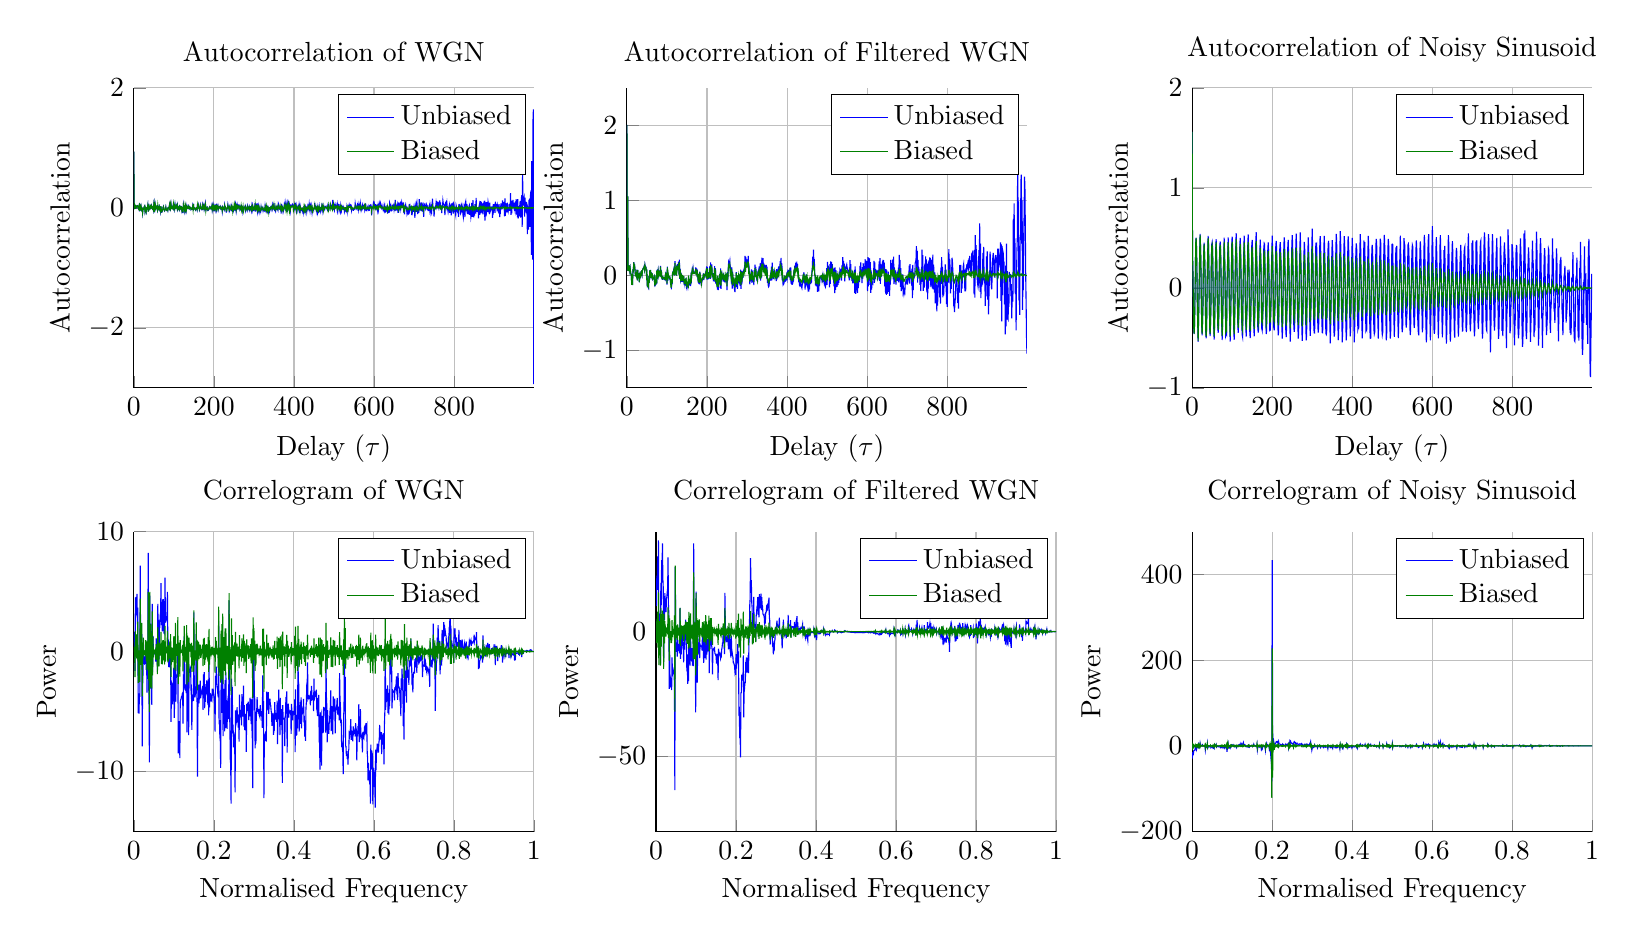
\begin{tikzpicture}

\begin{axis}[%
width=2in,
height=1.5in,
scale only axis,
xmin=0,
xmax=999,
xlabel={Delay ($\tau$)},
xmajorgrids,
ymin=-1.5,
ymax=2.5,
ylabel={Autocorrelation},
ymajorgrids,
name=plot3,
title={Autocorrelation of Filtered WGN},
axis x line*=bottom,
axis y line*=left,
legend style={draw=black,fill=white,legend cell align=left}
]
\addplot [color=blue,solid]
  table[row sep=crcr]{-999	-1.04363351459786\\
-998	-0.815393418274118\\
-997	-0.372948894421538\\
-996	-0.0103770255234643\\
-995	0.633423855500881\\
-994	1.18138138479025\\
-993	1.31502581509801\\
-992	0.815896416656528\\
-991	0.50363649253043\\
-990	-0.1953021425073\\
-989	-0.0623208969984734\\
-988	-0.460736844413034\\
-987	0.998697226826023\\
-986	0.422636304299663\\
-985	1.34394266846885\\
-984	1.25064180494122\\
-983	0.471963224087121\\
-982	0.510025065669935\\
-981	-0.525778308578391\\
-980	-0.203080960845305\\
-979	-0.33228967869119\\
-978	0.985319386508805\\
-977	0.581290893416081\\
-976	1.66264522154805\\
-975	0.50085929513947\\
-974	0.307686212046233\\
-973	-0.0524128016839269\\
-972	-0.732405975746396\\
-971	-0.0115030910098649\\
-970	-0.24900991326284\\
-969	0.493081953610079\\
-968	0.226574586899956\\
-967	0.958517276998491\\
-966	-0.00408138856109009\\
-965	0.753669296615314\\
-964	-0.348754301732965\\
-963	-0.205634581251323\\
-962	-0.326251373594918\\
-961	-0.574526521226671\\
-960	-0.117044334448687\\
-959	-0.276548538634285\\
-958	0.0132107040710342\\
-957	0.0130315032406713\\
-956	-0.0629114071239153\\
-955	0.0450849996345127\\
-954	-0.420282775980449\\
-953	-0.296492803302761\\
-952	-0.586472068895221\\
-951	-0.572449948068382\\
-950	0.057994671830281\\
-949	-0.589511655379882\\
-948	0.422506353218865\\
-947	-0.679105865398074\\
-946	0.13157833960864\\
-945	-0.785058994076771\\
-944	-0.095677851557563\\
-943	-0.3854161812548\\
-942	0.183950967371892\\
-941	0.137404060102939\\
-940	0.292227883752924\\
-939	0.31889582779064\\
-938	-0.262435176262816\\
-937	0.392937255991479\\
-936	-0.614163234633886\\
-935	0.412225226956488\\
-934	-0.339027290280635\\
-933	0.440815022040499\\
-932	0.102191742856405\\
-931	0.257516590021732\\
-930	0.201580682354975\\
-929	0.249374271159448\\
-928	0.357681880094559\\
-927	-0.0413467081156917\\
-926	0.355141967192458\\
-925	-0.307484370266039\\
-924	0.211177920410408\\
-923	0.172205980952393\\
-922	0.261217689458267\\
-921	0.263490775310009\\
-920	0.22390353455266\\
-919	-0.0327427805797715\\
-918	0.146858178152754\\
-917	0.0079437941785853\\
-916	0.212473584610194\\
-915	0.30039436898326\\
-914	0.251897835431449\\
-913	0.15975861323346\\
-912	-0.0449466316445\\
-911	-0.185500590871252\\
-910	-0.125240385695526\\
-909	0.0456877622607144\\
-908	0.177983490036617\\
-907	0.317156630209034\\
-906	-0.0371063312242737\\
-905	-0.092319610455751\\
-904	-0.307961396721437\\
-903	-0.518773409531226\\
-902	-0.0171870496984345\\
-901	-0.324642296503618\\
-900	0.321383389843046\\
-899	-0.1192067080648\\
-898	0.254574416414328\\
-897	-0.279329981886411\\
-896	-0.0256723603242004\\
-895	-0.405839921390248\\
-894	-0.0713724712295286\\
-893	-0.0813020517777816\\
-892	-0.0241487171389569\\
-891	0.381225012972074\\
-890	-0.0658432971270982\\
-889	0.300655315995305\\
-888	-0.121576186865806\\
-887	-0.0444570191510686\\
-886	-0.149990101624881\\
-885	0.0137040348258051\\
-884	-0.303406686864369\\
-883	0.424617330212631\\
-882	-0.219304594336568\\
-881	0.693825505716365\\
-880	0.0205901001278357\\
-879	0.335322280441673\\
-878	-0.102553062357567\\
-877	-0.152332835562867\\
-876	-0.117086699383064\\
-875	-0.0569560046778872\\
-874	0.170256267500391\\
-873	0.23131034764546\\
-872	0.402118150028732\\
-871	0.0331217112508355\\
-870	0.536646027242848\\
-869	-0.295635425135905\\
-868	0.341406904761206\\
-867	-0.254773314069943\\
-866	0.143287555260027\\
-865	-0.00147375030623251\\
-864	0.33127313042529\\
-863	0.249837696651866\\
-862	0.294584376495875\\
-861	0.283434931967355\\
-860	0.00624673992309011\\
-859	0.183634006352344\\
-858	0.0494383351678206\\
-857	0.172647903677639\\
-856	0.258491307169996\\
-855	0.0955983638793474\\
-854	0.226542554870719\\
-853	0.0833989317349563\\
-852	0.100222213414149\\
-851	0.145531991221578\\
-850	0.109239087194665\\
-849	0.14840599310295\\
-848	0.0432763585593717\\
-847	0.101466582559405\\
-846	-0.211559887963582\\
-845	-0.0120646809861329\\
-844	-0.214318803056287\\
-843	0.0772259974317009\\
-842	0.0437693054274404\\
-841	0.152671739260591\\
-840	0.124608241503215\\
-839	0.00948851911921479\\
-838	0.0252171040317903\\
-837	-0.177454846203651\\
-836	0.033937028718229\\
-835	-0.232262963388992\\
-834	0.14027334323948\\
-833	-0.029622249415874\\
-832	0.0483804289319053\\
-831	0.138105385346666\\
-830	-0.231096164905846\\
-829	-0.0743089172998092\\
-828	-0.444053323752499\\
-827	-0.250146456594666\\
-826	-0.365629542441597\\
-825	-0.187843414031856\\
-824	-0.0673701605432181\\
-823	-0.111242759504802\\
-822	-0.0290010480693421\\
-821	-0.172590382563087\\
-820	-0.318929015615383\\
-819	-0.390499066968244\\
-818	-0.489679813569858\\
-817	-0.353886180149101\\
-816	-0.370035871161104\\
-815	-0.0463527205972571\\
-814	0.0582833610749022\\
-813	0.172497244191376\\
-812	0.234564717677152\\
-811	0.0310669819868522\\
-810	-0.180477684920314\\
-809	-0.0580214063798645\\
-808	-0.240071399826351\\
-807	0.117447497572302\\
-806	0.218417366353082\\
-805	0.076523803352465\\
-804	0.35094394361032\\
-803	-0.0958865754402188\\
-802	-0.0585500562977668\\
-801	-0.078398610115434\\
-800	-0.421101398841462\\
-799	-0.0132609843021174\\
-798	-0.382390283664452\\
-797	0.0749426582208418\\
-796	-0.143254242171506\\
-795	0.147483725739245\\
-794	-0.0180492488533522\\
-793	-0.0149761029714219\\
-792	-0.141020431713003\\
-791	-0.268650201805541\\
-790	-0.146198272820216\\
-789	-0.293765082486601\\
-788	0.113125798836355\\
-787	-0.0878365230152614\\
-786	0.242536756872175\\
-785	-0.114485994621044\\
-784	0.102026277035956\\
-783	-0.375826116090936\\
-782	-0.00367579998958882\\
-781	-0.292333941609832\\
-780	-0.0200398305861199\\
-779	-0.0283385794625464\\
-778	-0.161253387720019\\
-777	-0.0558773354942843\\
-776	-0.402172620434134\\
-775	-0.195589912574743\\
-774	-0.480913956973914\\
-773	-0.121267784905008\\
-772	-0.374135776218247\\
-771	0.00637252874262444\\
-770	-0.374466687436208\\
-769	0.038749117662984\\
-768	-0.228565516514098\\
-767	-0.0333370971798334\\
-766	0.141991074311816\\
-765	-0.187836469650783\\
-764	0.277451334599427\\
-763	-0.174911865409052\\
-762	0.206805602410896\\
-761	-0.134917247970532\\
-760	0.178515038100089\\
-759	-0.157026211917172\\
-758	0.234097828942306\\
-757	-0.0691135266025139\\
-756	0.240268737582321\\
-755	-0.0264369041136323\\
-754	0.200072163991382\\
-753	-0.176287774996041\\
-752	0.155373085425498\\
-751	-0.320162411891588\\
-750	0.133245897228892\\
-749	-0.224059379058487\\
-748	0.213389760397435\\
-747	-0.0380900918181716\\
-746	0.253245739775719\\
-745	-0.0560623352441627\\
-744	0.155570969763806\\
-743	-0.162503597890283\\
-742	-0.0787216909796325\\
-741	-0.0469478111583977\\
-740	-0.206954993393662\\
-739	0.271216704442819\\
-738	-0.0819594193359097\\
-737	0.344242894494683\\
-736	-0.0856256139386184\\
-735	0.0879268839787315\\
-734	-0.210961371219659\\
-733	-0.0177473140889584\\
-732	-0.126477682278954\\
-731	0.0374735012215548\\
-730	0.0370407404103204\\
-729	0.106206182251417\\
-728	0.00864028234365415\\
-727	0.207555669246918\\
-726	-0.0974251583841542\\
-725	0.325628164360817\\
-724	0.0228516263248094\\
-723	0.390098567303832\\
-722	0.209946947187263\\
-721	0.181345268743806\\
-720	0.16695028393122\\
-719	-0.00648665552367264\\
-718	-0.0207021068818253\\
-717	0.00872690397768966\\
-716	0.0204860689190695\\
-715	-0.197550050560712\\
-714	0.139607537083428\\
-713	-0.30163646375727\\
-712	0.0911807976146714\\
-711	-0.136913387449996\\
-710	0.0598423378403371\\
-709	0.0114854893821284\\
-708	-0.0408170777916935\\
-707	0.149209391943998\\
-706	-0.110600816859829\\
-705	0.128136207337175\\
-704	-0.0447001379616759\\
-703	-0.0522841348679916\\
-702	-0.0126829161535802\\
-701	-0.122302168636536\\
-700	-0.0781314611297213\\
-699	-0.0586582579803318\\
-698	-0.0914834919591911\\
-697	-0.0729295699411848\\
-696	-0.092864520283798\\
-695	-0.121392278076231\\
-694	-0.227891970976494\\
-693	-0.210542326741654\\
-692	-0.245116675991139\\
-691	-0.188237043357705\\
-690	-0.216799937506776\\
-689	0.0140796560761454\\
-688	-0.186373222547489\\
-687	-0.0156624059431485\\
-686	-0.00473456597227443\\
-685	-0.208611455267537\\
-684	0.0977567308822029\\
-683	-0.15369249794411\\
-682	0.204866107585294\\
-681	-0.0457028662890265\\
-680	0.274590907540447\\
-679	-0.0935624187146587\\
-678	0.10432796564248\\
-677	-0.0651961322350344\\
-676	-0.0550953145517517\\
-675	-0.0110845679624149\\
-674	-0.0741480737395337\\
-673	0.00283736572255142\\
-672	-0.124405166668704\\
-671	0.0664965165230686\\
-670	-0.0899474481134355\\
-669	0.00904619618192852\\
-668	0.105380538354988\\
-667	-0.117167622017734\\
-666	0.250074807238321\\
-665	-0.0545382332464592\\
-664	0.210141662147127\\
-663	0.0384639283777349\\
-662	0.0925723747814932\\
-661	0.163793917658382\\
-660	0.032381808683531\\
-659	0.206878341296832\\
-658	-0.121830446554498\\
-657	-8.60381649881022e-05\\
-656	-0.271964632195568\\
-655	-0.00506609072092226\\
-654	-0.218637376246984\\
-653	0.0488370933927217\\
-652	-0.165671248784754\\
-651	-0.025702930453761\\
-650	-0.246028779738641\\
-649	0.0655475122921821\\
-648	-0.258496070894086\\
-647	0.0831993038157478\\
-646	-0.241576542423754\\
-645	0.0379512999143089\\
-644	-0.147909197400734\\
-643	0.169895208946157\\
-642	0.0679665594755405\\
-641	0.204473931476011\\
-640	0.148879604444391\\
-639	0.113600288191362\\
-638	0.148179117128455\\
-637	0.0702547036639643\\
-636	0.143433067837113\\
-635	-0.0190608063487476\\
-634	0.15457107025356\\
-633	-0.111771210395885\\
-632	0.228837170618131\\
-631	-0.071743104126098\\
-630	0.185941545882583\\
-629	0.0625693460930249\\
-628	0.0221401040886883\\
-627	0.0734860655811582\\
-626	-0.0673862035969657\\
-625	0.030321833114157\\
-624	0.0148781716745851\\
-623	0.0581122958396529\\
-622	0.0677636611538852\\
-621	0.049266310903724\\
-620	-0.0491740462003995\\
-619	0.173371480197314\\
-618	-0.101369027815569\\
-617	0.193152314035515\\
-616	-0.0355538447051377\\
-615	0.00359136627491825\\
-614	-0.109795044103616\\
-613	-0.100003957854625\\
-612	-0.118882216919753\\
-611	-0.188005409665871\\
-610	0.0651930541312509\\
-609	-0.232591394773502\\
-608	0.177607965965497\\
-607	-0.125952332579827\\
-606	0.226188591157512\\
-605	-0.0355798242633409\\
-604	0.230948100458757\\
-603	-0.148209546819232\\
-602	0.243725819168297\\
-601	-0.211174168946405\\
-600	0.189681081389456\\
-599	-0.0262464555726736\\
-598	0.0506105299402483\\
-597	0.194886111419383\\
-596	0.0435117761796245\\
-595	0.215822635178714\\
-594	0.0398136471574751\\
-593	0.0878534833610025\\
-592	0.0556882664943471\\
-591	0.0289924480184822\\
-590	0.163380128558339\\
-589	-0.0443773849659172\\
-588	0.108322830511996\\
-587	-0.104655697315082\\
-586	0.0731928479852909\\
-585	-0.0281463704386725\\
-584	0.172214594530663\\
-583	-0.0174309930635532\\
-582	0.126792345416806\\
-581	-0.0886010596602731\\
-580	-0.032008082296915\\
-579	-0.0283116362222452\\
-578	-0.168913808401335\\
-577	-0.0207419872232183\\
-576	-0.232285906769134\\
-575	-0.0821976997359977\\
-574	-0.171605136450106\\
-573	-0.134921041093445\\
-572	-0.015649557583459\\
-571	-0.246743209832358\\
-570	0.118842037607456\\
-569	-0.234531534224594\\
-568	0.0731062307869774\\
-567	-0.103291804073402\\
-566	-0.0470447722605344\\
-565	0.0172934754464709\\
-564	-0.106255587636175\\
-563	0.0279199426013876\\
-562	-0.0713382939923114\\
-561	0.00774918754642565\\
-560	0.00419334899963453\\
-559	0.150889270078587\\
-558	-0.0310635551654649\\
-557	0.204680402951894\\
-556	-0.0671215253862196\\
-555	0.0726454557985221\\
-554	-0.00617432910267686\\
-553	0.0307176278416534\\
-552	0.0520715671115544\\
-551	0.0947721568429137\\
-550	0.0936890069886494\\
-549	0.144627469641633\\
-548	0.127669914488629\\
-547	0.094894396893292\\
-546	0.039238881837479\\
-545	0.116280187207565\\
-544	-0.0783404716858793\\
-543	0.155265918350937\\
-542	0.0275090814999468\\
-541	0.192993379171168\\
-540	0.132375803666385\\
-539	0.243682212652897\\
-538	0.0242780100519294\\
-537	0.133109040167858\\
-536	-0.0706475678332248\\
-535	0.0883980458062734\\
-534	-0.00742920311421823\\
-533	0.0470888301811684\\
-532	0.0660012241868136\\
-531	-0.0636814869732107\\
-530	0.0502705871189139\\
-529	-0.100183221263006\\
-528	0.0035955406519815\\
-527	-0.129881440332815\\
-526	-0.0279191087412514\\
-525	-0.152248751501673\\
-524	0.0134654277334169\\
-523	-0.157377144267124\\
-522	0.0714532677784389\\
-521	-0.191554709460392\\
-520	0.105556347326613\\
-519	-0.238125986381746\\
-518	0.100457152242553\\
-517	-0.146127420049394\\
-516	0.00670332097091019\\
-515	0.0492814353566478\\
-514	-0.0061836006202535\\
-513	0.150320374889297\\
-512	0.0694512038880981\\
-511	0.176100397479238\\
-510	0.0471274099684376\\
-509	0.186669921360365\\
-508	-0.112304020208373\\
-507	0.148903114847071\\
-506	-0.16041310530124\\
-505	0.107584575355066\\
-504	0.0405497923755594\\
-503	0.129635083685404\\
-502	0.0422386447405541\\
-501	0.179422271239003\\
-500	-0.127234847436161\\
-499	0.0966428207434955\\
-498	-0.0867029521006854\\
-497	-0.115185498669592\\
-496	-0.056151515511808\\
-495	-0.143885978970001\\
-494	-0.127295880880691\\
-493	-0.0250558658864456\\
-492	-0.0728947600448959\\
-491	-0.0300826228508302\\
-490	0.00163415116640336\\
-489	-0.0889010452957629\\
-488	-0.0174997416213614\\
-487	-0.0680713145499883\\
-486	-0.0353847389491655\\
-485	-0.0126716602442486\\
-484	-0.0245235424952779\\
-483	-0.0292520427707615\\
-482	-0.0509104305956739\\
-481	-0.136204886977032\\
-480	-0.0903926493319941\\
-479	-0.213470393871124\\
-478	-0.178789124219512\\
-477	-0.123477290374779\\
-476	-0.220143919503695\\
-475	-0.0629526679797923\\
-474	-0.0934886825771027\\
-473	-0.145595438888114\\
-472	-0.0752171760732223\\
-471	-0.132342925812069\\
-470	-0.0172877532127258\\
-469	0.0256066714734926\\
-468	0.21640426281275\\
-467	0.120712407427533\\
-466	0.341517043401084\\
-465	0.167672531379741\\
-464	0.244823898291092\\
-463	0.10155791652107\\
-462	0.047508399989672\\
-461	-0.0742979407713487\\
-460	-0.0570849738965563\\
-459	-0.0578257594754937\\
-458	-0.115826520292563\\
-457	-0.0333210584573663\\
-456	-0.187375297574722\\
-455	-0.0967052409045339\\
-454	-0.217607619709352\\
-453	-0.134940335813021\\
-452	-0.172133177769243\\
-451	-0.131042341341243\\
-450	-0.0283511531102268\\
-449	-0.0913281903057196\\
-448	0.0142053686157023\\
-447	-0.149339303380931\\
-446	-0.0633782297487008\\
-445	-0.191115153412443\\
-444	-0.0176901680547446\\
-443	-0.107111469237644\\
-442	0.0429177541482039\\
-441	-0.0293783187094339\\
-440	-0.0170237647131021\\
-439	-0.0921448344607363\\
-438	-0.11886108410245\\
-437	-0.168382219300048\\
-436	-0.150510107770763\\
-435	-0.138615341771446\\
-434	-0.10661100697887\\
-433	-0.12589942294672\\
-432	-0.108074865242562\\
-431	-0.123677800333416\\
-430	-0.0642499109046386\\
-429	-0.0706556124967429\\
-428	0.0638788390605739\\
-427	0.0126450091327192\\
-426	0.153590076265782\\
-425	0.120465031292617\\
-424	0.165845025405849\\
-423	0.154135470411936\\
-422	0.10759339469779\\
-421	0.13118146418264\\
-420	0.0642091599352602\\
-419	0.125890440525358\\
-418	0.0246690048477848\\
-417	0.0654600258676778\\
-416	-0.0564632835535846\\
-415	-0.0435797302440827\\
-414	-0.107663760829703\\
-413	-0.118745150866733\\
-412	-0.118902404796852\\
-411	-0.013239148280661\\
-410	-0.112115302963194\\
-409	0.107400818164292\\
-408	-0.0646727661451931\\
-407	0.103365831244846\\
-406	-0.0259997798803164\\
-405	0.0697912034263317\\
-404	0.0131424735486226\\
-403	0.0383083883469368\\
-402	0.00880008940820691\\
-401	0.0323302064190248\\
-400	-0.0381255330871025\\
-399	-0.00432061429014373\\
-398	-0.0534096481340085\\
-397	-0.064326403355663\\
-396	-0.0379032784611924\\
-395	-0.0604426605046968\\
-394	-0.036054627622287\\
-393	-0.0734737080474841\\
-392	-0.111534041969672\\
-391	-0.118891974961638\\
-390	-0.127390861041465\\
-389	-0.00158308833206266\\
-388	-0.0648594139006499\\
-387	0.160826874425125\\
-386	0.00647014323847761\\
-385	0.231547805976654\\
-384	0.0971626283293954\\
-383	0.190927932834994\\
-382	0.123140259012826\\
-381	0.102238882360649\\
-380	0.0389494338830141\\
-379	0.12061822174384\\
-378	-0.0275679094277413\\
-377	0.0646579639192797\\
-376	0.0410342723513924\\
-375	-0.0532203121776232\\
-374	0.0826813800884705\\
-373	-0.0763447498504959\\
-372	0.00258614282820339\\
-371	-0.0266253962093189\\
-370	-0.0105251643719949\\
-369	0.0681095622277292\\
-368	-0.00781540909134312\\
-367	0.060030049936706\\
-366	-0.0509930966273133\\
-365	0.0874727129140728\\
-364	-0.036577316270435\\
-363	0.170687188426994\\
-362	-0.0667969942512456\\
-361	0.115654343536955\\
-360	-0.069303282763808\\
-359	0.0177102297398312\\
-358	-0.015350256527936\\
-357	-0.064247947876866\\
-356	-0.0696154584440945\\
-355	-0.13969120741591\\
-354	-0.15204287107578\\
-353	-0.135022697029114\\
-352	-0.0727257180939212\\
-351	-0.0798738899972572\\
-350	0.115908763325047\\
-349	-0.0445151829179148\\
-348	0.140788513419813\\
-347	-0.0024876413581307\\
-346	0.106020902364141\\
-345	0.0593171179784411\\
-344	0.141388397979843\\
-343	0.0392165041205666\\
-342	0.159651872668595\\
-341	0.0687321432858777\\
-340	0.221240200238566\\
-339	0.219687109941465\\
-338	0.154893265716913\\
-337	0.236539852337069\\
-336	-0.0304188311506921\\
-335	0.167966383672038\\
-334	-0.070445117570371\\
-333	0.160953255902271\\
-332	-0.0404801848410547\\
-331	0.120042137769742\\
-330	0.016182409844642\\
-329	0.0636467151406772\\
-328	0.0282520173730935\\
-327	0.03832603246326\\
-326	-0.0862089700537686\\
-325	-0.0292820789080909\\
-324	-0.0448923940621195\\
-323	-0.0146183721958273\\
-322	0.112084830750243\\
-321	0.0509774553601651\\
-320	0.14220598570714\\
-319	-0.0198259477881476\\
-318	0.0686351195552827\\
-317	-0.130537334645821\\
-316	-0.0154449478465503\\
-315	-0.0824882458604439\\
-314	-0.080461772359904\\
-313	0.0636744456243459\\
-312	-0.0985175595282143\\
-311	0.0800988542483286\\
-310	-0.00196911543268269\\
-309	-0.0722073961978562\\
-308	0.0213606589796812\\
-307	-0.120773953299136\\
-306	-0.0135315568201781\\
-305	0.10100674905661\\
-304	0.0767774668646748\\
-303	0.260661785255525\\
-302	0.151230214653581\\
-301	0.212221497254165\\
-300	0.164263474528681\\
-299	0.158964718803385\\
-298	0.153748681966071\\
-297	0.246668414121229\\
-296	0.0643604451622279\\
-295	0.259847761649349\\
-294	0.0531707636326976\\
-293	0.0909537044457016\\
-292	0.069917998126588\\
-291	0.0660696060715637\\
-290	-0.0332206317883896\\
-289	0.0535083502060757\\
-288	-0.0416229968921667\\
-287	-0.118635386956455\\
-286	0.0601460079488946\\
-285	-0.179659644849917\\
-284	0.077317205369157\\
-283	-0.140559880783286\\
-282	0.0133306433398583\\
-281	-0.0803215709857943\\
-280	-0.0480159008266721\\
-279	-0.00151892940739528\\
-278	-0.107871486889191\\
-277	-0.0164839876419328\\
-276	-0.179333334665256\\
-275	0.00279112899516333\\
-274	-0.157187999417667\\
-273	0.0436488492288501\\
-272	-0.148494176083181\\
-271	-0.0448382709079089\\
-270	-0.221449166380465\\
-269	-0.118367772513843\\
-268	-0.161588230024726\\
-267	-0.125958471390317\\
-266	-0.0387622149445972\\
-265	-0.135809125908628\\
-264	0.0498714918567412\\
-263	-0.177774206914042\\
-262	0.106417075931887\\
-261	-0.111283953049953\\
-260	0.0759331090307746\\
-259	0.101198733213534\\
-258	0.0561375712075762\\
-257	0.190198323853867\\
-256	0.158702636037994\\
-255	0.1511095136889\\
-254	0.172809140795804\\
-253	0.085290472378727\\
-252	-0.0701648570998585\\
-251	0.0418230943048738\\
-250	-0.196117952376165\\
-249	0.0253677380149616\\
-248	-0.0926133747172275\\
-247	-0.0126216271278218\\
-246	-0.0715849705749812\\
-245	-0.0214854727062282\\
-244	-0.0912737302018361\\
-243	0.00469032026600658\\
-242	-0.0815132075866314\\
-241	-0.0105523925549729\\
-240	-0.0411700375148754\\
-239	-0.0259098541537948\\
-238	0.0135285929071386\\
-237	-0.0824425105392952\\
-236	0.0521541478757303\\
-235	-0.178770222622829\\
-234	0.0923338472220928\\
-233	-0.167097685326355\\
-232	0.0217581211784663\\
-231	-0.110792961517042\\
-230	-0.107166417290001\\
-229	-0.0463748961886978\\
-228	-0.197690327305036\\
-227	-0.00580711873661304\\
-226	-0.189387027095872\\
-225	-0.0722344603964152\\
-224	-0.128861137474299\\
-223	-0.063293237646316\\
-222	-0.110567220392975\\
-221	0.0980566579837259\\
-220	-0.0854730391526121\\
-219	0.122133496182033\\
-218	-0.0597220420317676\\
-217	0.0301339755442529\\
-216	-0.0796079903216469\\
-215	0.0201057094653965\\
-214	0.0238467617957407\\
-213	0.00545158010135406\\
-212	0.147431759049758\\
-211	0.0595882391177864\\
-210	0.0364536245933713\\
-209	0.171778553948424\\
-208	-0.0464304595278989\\
-207	0.11967158738872\\
-206	-0.0281805750605865\\
-205	0.0319724419094905\\
-204	-0.0449509351578904\\
-203	0.0435120542819007\\
-202	-0.0547011488250916\\
-201	0.112009185426442\\
-200	-0.0578887337452099\\
-199	0.118634361361266\\
-198	-0.0323338747407007\\
-197	0.0461047794766446\\
-196	0.0234936763588192\\
-195	-0.0024893389411989\\
-194	-0.0066373103310587\\
-193	0.0045798650805042\\
-192	-0.0641853224242818\\
-191	0.0269401134670081\\
-190	-0.031028104614798\\
-189	-0.0360675267936719\\
-188	-0.0672392408780297\\
-187	-0.0832885859503791\\
-186	-0.138491927353381\\
-185	-0.0755711411492776\\
-184	-0.0338089362921981\\
-183	-0.103437554271849\\
-182	0.0481611754166706\\
-181	-0.120468818504238\\
-180	0.0151525985588763\\
-179	-0.11124521064539\\
-178	0.019722165199779\\
-177	-0.0232308897563331\\
-176	0.0418255805108938\\
-175	0.0203178661061408\\
-174	0.0938971999915839\\
-173	0.00292757335583014\\
-172	0.105077163303892\\
-171	0.0471057252447578\\
-170	0.0528566810805744\\
-169	0.0285889307866693\\
-168	0.0294752468004741\\
-167	0.0319765622127797\\
-166	0.0290663616135366\\
-165	0.0939739411313917\\
-164	0.0544023059418741\\
-163	0.0765088286581258\\
-162	0.0364836653103949\\
-161	-0.0552602958102783\\
-160	-0.0248333235644841\\
-159	-0.143430778485294\\
-158	-0.0718595856711487\\
-157	-0.0823257068423137\\
-156	-0.103059728085714\\
-155	-0.0650022689935252\\
-154	-0.13389524081638\\
-153	-0.0771235295366499\\
-152	-0.147067034724923\\
-151	-0.113606520323097\\
-150	-0.108550013120893\\
-149	-0.143835774279284\\
-148	-0.0754631179280989\\
-147	-0.101366977307711\\
-146	-0.0778057254512771\\
-145	-0.115431886144741\\
-144	-0.0552222883709299\\
-143	-0.130217511960649\\
-142	-0.0138501063056188\\
-141	-0.0917683019186468\\
-140	-0.00626147718878808\\
-139	-0.0873389420846605\\
-138	0.00640534486627103\\
-137	-0.0868474479362875\\
-136	-0.00873342995839129\\
-135	-0.033943440857821\\
-134	-0.0581354010230789\\
-133	0.0882067769075481\\
-132	-0.0477665454515415\\
-131	0.208257251421964\\
-130	0.0109958762991628\\
-129	0.183877048612003\\
-128	0.0764900401932535\\
-127	0.14911905717787\\
-126	0.0799082646137254\\
-125	0.143225953097721\\
-124	-0.00306740049477434\\
-123	0.0819796937873217\\
-122	0.042303843006832\\
-121	0.0306020517950055\\
-120	0.188112323654164\\
-119	0.000491797362104517\\
-118	0.120680116955786\\
-117	0.0372868653975865\\
-116	0.0537232473505195\\
-115	0.0247264234742079\\
-114	0.0322244516511055\\
-113	-0.119441428084153\\
-112	-0.0626577241969367\\
-111	-0.18499223864241\\
-110	-0.0576195886550194\\
-109	-0.107217736719664\\
-108	-0.0440292816790989\\
-107	-0.0249740161598221\\
-106	-0.0378075579981581\\
-105	-0.0246501878996028\\
-104	-0.0170044466596933\\
-103	0.0250666246271362\\
-102	-0.0718331673545915\\
-101	0.117028131073322\\
-100	-0.121770699533439\\
-99	0.0359882396672716\\
-98	-0.0584451656621185\\
-97	-0.0585311616163053\\
-96	-0.00826453347747701\\
-95	-0.0568612477038494\\
-94	-0.046609859370896\\
-93	-0.0503741324734114\\
-92	-0.0314453217338547\\
-91	-0.0332994560380093\\
-90	-0.024674500472136\\
-89	-0.0516410677393995\\
-88	-0.0508088195473588\\
-87	-0.0291294527926572\\
-86	0.0661595703189276\\
-85	-0.0022984589175748\\
-84	0.125869901652185\\
-83	-0.024465646307259\\
-82	0.0661878124034748\\
-81	-0.00562567064121403\\
-80	0.0663277297850711\\
-79	0.0134320884262418\\
-78	0.0665838441640203\\
-77	0.02058408591205\\
-76	0.0791526956539579\\
-75	-0.0387718960884523\\
-74	-0.00500454778880552\\
-73	-0.115519466188512\\
-72	-0.113623660517647\\
-71	-0.126208744628982\\
-70	-0.0586826610126015\\
-69	-0.0932039257278569\\
-68	-0.0218700405570183\\
-67	-0.0409339626178173\\
-66	-0.039348645061776\\
-65	-0.0481170765091857\\
-64	-0.00958346909664462\\
-63	-0.0379121192130143\\
-62	-0.0179159292304408\\
-61	0.0400557428651967\\
-60	-0.0352338151067965\\
-59	0.0735049343983383\\
-58	-0.0319636532207356\\
-57	0.065834615365273\\
-56	-0.10111194965723\\
-55	-0.00932092777047381\\
-54	-0.167335306191132\\
-53	-0.154605849592684\\
-52	-0.107908239614522\\
-51	-0.158593405730717\\
-50	0.0198795846641712\\
-49	-0.00669527020813078\\
-48	0.100853524307399\\
-47	0.113375514245935\\
-46	0.10260692679183\\
-45	0.137314550993774\\
-44	0.0803584517200142\\
-43	0.120449254235359\\
-42	0.103115446368568\\
-41	0.0977726203009288\\
-40	0.0894314602829086\\
-39	0.0702031737770385\\
-38	0.0200883735018632\\
-37	0.0674375821194236\\
-36	-0.00594482382568309\\
-35	0.0533452998150266\\
-34	-0.0186781858071727\\
-33	-0.0305556730616651\\
-32	-0.00447875522991109\\
-31	-0.0916551204950295\\
-30	0.0280178276826789\\
-29	-0.027686208994281\\
-28	-0.0308236488308933\\
-27	0.0721394981482458\\
-26	-0.0665723451240716\\
-25	0.0757438182345833\\
-24	-0.0225229856209991\\
-23	-0.0107877327601332\\
-22	0.0225830790277231\\
-21	0.012250207050634\\
-20	0.0862469520584132\\
-19	0.139093627995982\\
-18	0.138059157858124\\
-17	0.174969623639052\\
-16	0.0419740612965344\\
-15	0.0812454923263921\\
-14	-0.129276662658293\\
-13	0.00277898977593677\\
-12	-0.126548363012727\\
-11	0.0123613463482388\\
-10	0.015055381201447\\
-9	0.0463455973248565\\
-8	0.0983231304904412\\
-7	0.0671684330870433\\
-6	0.13261775947866\\
-5	0.0588308503002559\\
-4	0.134854102151819\\
-3	0.0611154265071904\\
-2	1.05481719408915\\
-1	0.0650618432594144\\
0	2.00756555636676\\
1	0.0650618432594143\\
2	1.05481719408915\\
3	0.0611154265071904\\
4	0.134854102151819\\
5	0.0588308503002559\\
6	0.13261775947866\\
7	0.0671684330870433\\
8	0.0983231304904412\\
9	0.0463455973248565\\
10	0.015055381201447\\
11	0.0123613463482388\\
12	-0.126548363012727\\
13	0.00277898977593676\\
14	-0.129276662658293\\
15	0.0812454923263921\\
16	0.0419740612965344\\
17	0.174969623639052\\
18	0.138059157858124\\
19	0.139093627995982\\
20	0.0862469520584132\\
21	0.012250207050634\\
22	0.0225830790277231\\
23	-0.0107877327601332\\
24	-0.0225229856209991\\
25	0.0757438182345833\\
26	-0.0665723451240715\\
27	0.0721394981482458\\
28	-0.0308236488308933\\
29	-0.027686208994281\\
30	0.0280178276826789\\
31	-0.0916551204950295\\
32	-0.00447875522991109\\
33	-0.0305556730616651\\
34	-0.0186781858071727\\
35	0.0533452998150266\\
36	-0.00594482382568306\\
37	0.0674375821194236\\
38	0.0200883735018632\\
39	0.0702031737770385\\
40	0.0894314602829086\\
41	0.0977726203009289\\
42	0.103115446368568\\
43	0.120449254235359\\
44	0.0803584517200142\\
45	0.137314550993774\\
46	0.10260692679183\\
47	0.113375514245935\\
48	0.100853524307399\\
49	-0.0066952702081308\\
50	0.0198795846641712\\
51	-0.158593405730717\\
52	-0.107908239614522\\
53	-0.154605849592684\\
54	-0.167335306191132\\
55	-0.00932092777047379\\
56	-0.10111194965723\\
57	0.065834615365273\\
58	-0.0319636532207355\\
59	0.0735049343983383\\
60	-0.0352338151067964\\
61	0.0400557428651967\\
62	-0.0179159292304408\\
63	-0.0379121192130143\\
64	-0.00958346909664462\\
65	-0.0481170765091857\\
66	-0.039348645061776\\
67	-0.0409339626178174\\
68	-0.0218700405570183\\
69	-0.0932039257278569\\
70	-0.0586826610126015\\
71	-0.126208744628982\\
72	-0.113623660517647\\
73	-0.115519466188512\\
74	-0.00500454778880554\\
75	-0.0387718960884523\\
76	0.0791526956539579\\
77	0.02058408591205\\
78	0.0665838441640203\\
79	0.0134320884262418\\
80	0.0663277297850711\\
81	-0.00562567064121403\\
82	0.0661878124034748\\
83	-0.024465646307259\\
84	0.125869901652185\\
85	-0.00229845891757478\\
86	0.0661595703189277\\
87	-0.0291294527926572\\
88	-0.0508088195473588\\
89	-0.0516410677393995\\
90	-0.024674500472136\\
91	-0.0332994560380093\\
92	-0.0314453217338547\\
93	-0.0503741324734114\\
94	-0.046609859370896\\
95	-0.0568612477038494\\
96	-0.00826453347747701\\
97	-0.0585311616163053\\
98	-0.0584451656621185\\
99	0.0359882396672716\\
100	-0.121770699533439\\
101	0.117028131073322\\
102	-0.0718331673545915\\
103	0.0250666246271362\\
104	-0.0170044466596934\\
105	-0.0246501878996028\\
106	-0.0378075579981581\\
107	-0.0249740161598221\\
108	-0.0440292816790989\\
109	-0.107217736719664\\
110	-0.0576195886550194\\
111	-0.18499223864241\\
112	-0.0626577241969367\\
113	-0.119441428084153\\
114	0.0322244516511055\\
115	0.0247264234742079\\
116	0.0537232473505195\\
117	0.0372868653975865\\
118	0.120680116955786\\
119	0.000491797362104533\\
120	0.188112323654164\\
121	0.0306020517950055\\
122	0.042303843006832\\
123	0.0819796937873216\\
124	-0.00306740049477436\\
125	0.143225953097721\\
126	0.0799082646137254\\
127	0.14911905717787\\
128	0.0764900401932535\\
129	0.183877048612003\\
130	0.0109958762991628\\
131	0.208257251421964\\
132	-0.0477665454515415\\
133	0.0882067769075481\\
134	-0.0581354010230789\\
135	-0.0339434408578209\\
136	-0.00873342995839129\\
137	-0.0868474479362874\\
138	0.00640534486627101\\
139	-0.0873389420846605\\
140	-0.00626147718878808\\
141	-0.0917683019186468\\
142	-0.0138501063056188\\
143	-0.130217511960649\\
144	-0.0552222883709299\\
145	-0.115431886144741\\
146	-0.0778057254512772\\
147	-0.101366977307711\\
148	-0.0754631179280989\\
149	-0.143835774279284\\
150	-0.108550013120893\\
151	-0.113606520323097\\
152	-0.147067034724923\\
153	-0.0771235295366499\\
154	-0.13389524081638\\
155	-0.0650022689935252\\
156	-0.103059728085714\\
157	-0.0823257068423137\\
158	-0.0718595856711487\\
159	-0.143430778485294\\
160	-0.0248333235644841\\
161	-0.0552602958102783\\
162	0.0364836653103949\\
163	0.0765088286581258\\
164	0.0544023059418741\\
165	0.0939739411313917\\
166	0.0290663616135366\\
167	0.0319765622127797\\
168	0.0294752468004741\\
169	0.0285889307866693\\
170	0.0528566810805744\\
171	0.0471057252447578\\
172	0.105077163303892\\
173	0.00292757335583012\\
174	0.0938971999915839\\
175	0.0203178661061408\\
176	0.0418255805108938\\
177	-0.0232308897563332\\
178	0.0197221651997789\\
179	-0.11124521064539\\
180	0.0151525985588763\\
181	-0.120468818504238\\
182	0.0481611754166706\\
183	-0.103437554271849\\
184	-0.0338089362921981\\
185	-0.0755711411492776\\
186	-0.13849192735338\\
187	-0.0832885859503791\\
188	-0.0672392408780297\\
189	-0.0360675267936719\\
190	-0.031028104614798\\
191	0.0269401134670081\\
192	-0.0641853224242818\\
193	0.0045798650805042\\
194	-0.00663731033105864\\
195	-0.00248933894119889\\
196	0.0234936763588192\\
197	0.0461047794766446\\
198	-0.0323338747407007\\
199	0.118634361361266\\
200	-0.0578887337452099\\
201	0.112009185426442\\
202	-0.0547011488250916\\
203	0.0435120542819007\\
204	-0.0449509351578903\\
205	0.0319724419094905\\
206	-0.0281805750605865\\
207	0.11967158738872\\
208	-0.0464304595278989\\
209	0.171778553948424\\
210	0.0364536245933713\\
211	0.0595882391177864\\
212	0.147431759049758\\
213	0.00545158010135405\\
214	0.0238467617957407\\
215	0.0201057094653965\\
216	-0.0796079903216469\\
217	0.0301339755442529\\
218	-0.0597220420317676\\
219	0.122133496182033\\
220	-0.0854730391526121\\
221	0.0980566579837259\\
222	-0.110567220392975\\
223	-0.063293237646316\\
224	-0.128861137474299\\
225	-0.0722344603964152\\
226	-0.189387027095872\\
227	-0.00580711873661305\\
228	-0.197690327305036\\
229	-0.0463748961886978\\
230	-0.107166417290001\\
231	-0.110792961517042\\
232	0.0217581211784663\\
233	-0.167097685326355\\
234	0.0923338472220928\\
235	-0.178770222622829\\
236	0.0521541478757303\\
237	-0.0824425105392952\\
238	0.0135285929071386\\
239	-0.0259098541537949\\
240	-0.0411700375148754\\
241	-0.0105523925549729\\
242	-0.0815132075866314\\
243	0.0046903202660066\\
244	-0.0912737302018361\\
245	-0.0214854727062282\\
246	-0.0715849705749812\\
247	-0.0126216271278218\\
248	-0.0926133747172276\\
249	0.0253677380149617\\
250	-0.196117952376165\\
251	0.0418230943048738\\
252	-0.0701648570998586\\
253	0.085290472378727\\
254	0.172809140795804\\
255	0.1511095136889\\
256	0.158702636037994\\
257	0.190198323853867\\
258	0.0561375712075762\\
259	0.101198733213534\\
260	0.0759331090307746\\
261	-0.111283953049953\\
262	0.106417075931887\\
263	-0.177774206914042\\
264	0.0498714918567412\\
265	-0.135809125908628\\
266	-0.0387622149445972\\
267	-0.125958471390317\\
268	-0.161588230024726\\
269	-0.118367772513843\\
270	-0.221449166380465\\
271	-0.0448382709079088\\
272	-0.148494176083181\\
273	0.0436488492288501\\
274	-0.157187999417667\\
275	0.00279112899516329\\
276	-0.179333334665256\\
277	-0.0164839876419327\\
278	-0.107871486889191\\
279	-0.0015189294073953\\
280	-0.0480159008266721\\
281	-0.0803215709857942\\
282	0.0133306433398582\\
283	-0.140559880783286\\
284	0.077317205369157\\
285	-0.179659644849917\\
286	0.0601460079488946\\
287	-0.118635386956455\\
288	-0.0416229968921667\\
289	0.0535083502060757\\
290	-0.0332206317883895\\
291	0.0660696060715637\\
292	0.069917998126588\\
293	0.0909537044457017\\
294	0.0531707636326976\\
295	0.259847761649349\\
296	0.0643604451622279\\
297	0.246668414121229\\
298	0.153748681966071\\
299	0.158964718803385\\
300	0.164263474528681\\
301	0.212221497254165\\
302	0.151230214653581\\
303	0.260661785255525\\
304	0.0767774668646747\\
305	0.10100674905661\\
306	-0.0135315568201782\\
307	-0.120773953299136\\
308	0.0213606589796812\\
309	-0.0722073961978562\\
310	-0.0019691154326827\\
311	0.0800988542483286\\
312	-0.0985175595282143\\
313	0.0636744456243458\\
314	-0.080461772359904\\
315	-0.0824882458604439\\
316	-0.0154449478465502\\
317	-0.130537334645821\\
318	0.0686351195552827\\
319	-0.0198259477881476\\
320	0.14220598570714\\
321	0.050977455360165\\
322	0.112084830750243\\
323	-0.0146183721958273\\
324	-0.0448923940621194\\
325	-0.0292820789080909\\
326	-0.0862089700537686\\
327	0.0383260324632599\\
328	0.0282520173730935\\
329	0.0636467151406771\\
330	0.016182409844642\\
331	0.120042137769742\\
332	-0.0404801848410548\\
333	0.160953255902271\\
334	-0.0704451175703711\\
335	0.167966383672038\\
336	-0.0304188311506921\\
337	0.236539852337069\\
338	0.154893265716913\\
339	0.219687109941465\\
340	0.221240200238566\\
341	0.0687321432858777\\
342	0.159651872668595\\
343	0.0392165041205667\\
344	0.141388397979843\\
345	0.0593171179784412\\
346	0.106020902364141\\
347	-0.00248764135813072\\
348	0.140788513419813\\
349	-0.0445151829179148\\
350	0.115908763325047\\
351	-0.0798738899972572\\
352	-0.0727257180939212\\
353	-0.135022697029114\\
354	-0.15204287107578\\
355	-0.13969120741591\\
356	-0.0696154584440945\\
357	-0.064247947876866\\
358	-0.015350256527936\\
359	0.0177102297398312\\
360	-0.069303282763808\\
361	0.115654343536955\\
362	-0.0667969942512456\\
363	0.170687188426994\\
364	-0.036577316270435\\
365	0.0874727129140728\\
366	-0.0509930966273133\\
367	0.060030049936706\\
368	-0.0078154090913431\\
369	0.0681095622277292\\
370	-0.0105251643719949\\
371	-0.0266253962093189\\
372	0.00258614282820343\\
373	-0.0763447498504959\\
374	0.0826813800884704\\
375	-0.0532203121776232\\
376	0.0410342723513925\\
377	0.0646579639192798\\
378	-0.0275679094277413\\
379	0.12061822174384\\
380	0.0389494338830141\\
381	0.102238882360649\\
382	0.123140259012826\\
383	0.190927932834994\\
384	0.0971626283293954\\
385	0.231547805976654\\
386	0.00647014323847754\\
387	0.160826874425125\\
388	-0.0648594139006499\\
389	-0.00158308833206267\\
390	-0.127390861041465\\
391	-0.118891974961638\\
392	-0.111534041969672\\
393	-0.0734737080474841\\
394	-0.036054627622287\\
395	-0.0604426605046968\\
396	-0.0379032784611924\\
397	-0.064326403355663\\
398	-0.0534096481340085\\
399	-0.00432061429014373\\
400	-0.0381255330871025\\
401	0.0323302064190248\\
402	0.00880008940820694\\
403	0.0383083883469368\\
404	0.0131424735486226\\
405	0.0697912034263317\\
406	-0.0259997798803164\\
407	0.103365831244846\\
408	-0.064672766145193\\
409	0.107400818164292\\
410	-0.112115302963194\\
411	-0.0132391482806611\\
412	-0.118902404796852\\
413	-0.118745150866733\\
414	-0.107663760829703\\
415	-0.0435797302440827\\
416	-0.0564632835535846\\
417	0.0654600258676778\\
418	0.0246690048477848\\
419	0.125890440525358\\
420	0.0642091599352602\\
421	0.13118146418264\\
422	0.10759339469779\\
423	0.154135470411936\\
424	0.165845025405849\\
425	0.120465031292617\\
426	0.153590076265782\\
427	0.0126450091327192\\
428	0.0638788390605739\\
429	-0.070655612496743\\
430	-0.0642499109046385\\
431	-0.123677800333416\\
432	-0.108074865242561\\
433	-0.12589942294672\\
434	-0.10661100697887\\
435	-0.138615341771446\\
436	-0.150510107770763\\
437	-0.168382219300048\\
438	-0.11886108410245\\
439	-0.0921448344607363\\
440	-0.0170237647131021\\
441	-0.029378318709434\\
442	0.0429177541482039\\
443	-0.107111469237644\\
444	-0.0176901680547446\\
445	-0.191115153412443\\
446	-0.0633782297487008\\
447	-0.149339303380931\\
448	0.0142053686157023\\
449	-0.0913281903057195\\
450	-0.0283511531102268\\
451	-0.131042341341243\\
452	-0.172133177769243\\
453	-0.134940335813021\\
454	-0.217607619709352\\
455	-0.0967052409045339\\
456	-0.187375297574722\\
457	-0.0333210584573663\\
458	-0.115826520292563\\
459	-0.0578257594754937\\
460	-0.0570849738965563\\
461	-0.0742979407713487\\
462	0.047508399989672\\
463	0.10155791652107\\
464	0.244823898291092\\
465	0.167672531379741\\
466	0.341517043401084\\
467	0.120712407427533\\
468	0.21640426281275\\
469	0.0256066714734926\\
470	-0.0172877532127258\\
471	-0.132342925812069\\
472	-0.0752171760732223\\
473	-0.145595438888114\\
474	-0.0934886825771026\\
475	-0.0629526679797923\\
476	-0.220143919503695\\
477	-0.123477290374779\\
478	-0.178789124219512\\
479	-0.213470393871124\\
480	-0.0903926493319941\\
481	-0.136204886977032\\
482	-0.050910430595674\\
483	-0.0292520427707615\\
484	-0.0245235424952779\\
485	-0.0126716602442486\\
486	-0.0353847389491655\\
487	-0.0680713145499883\\
488	-0.0174997416213614\\
489	-0.0889010452957629\\
490	0.00163415116640338\\
491	-0.0300826228508302\\
492	-0.0728947600448959\\
493	-0.0250558658864456\\
494	-0.127295880880691\\
495	-0.14388597897\\
496	-0.056151515511808\\
497	-0.115185498669592\\
498	-0.0867029521006854\\
499	0.0966428207434955\\
500	-0.127234847436161\\
501	0.179422271239003\\
502	0.0422386447405541\\
503	0.129635083685404\\
504	0.0405497923755595\\
505	0.107584575355066\\
506	-0.16041310530124\\
507	0.148903114847071\\
508	-0.112304020208373\\
509	0.186669921360365\\
510	0.0471274099684375\\
511	0.176100397479238\\
512	0.0694512038880981\\
513	0.150320374889297\\
514	-0.00618360062025335\\
515	0.0492814353566478\\
516	0.00670332097091018\\
517	-0.146127420049394\\
518	0.100457152242553\\
519	-0.238125986381746\\
520	0.105556347326613\\
521	-0.191554709460392\\
522	0.0714532677784389\\
523	-0.157377144267124\\
524	0.0134654277334169\\
525	-0.152248751501673\\
526	-0.0279191087412514\\
527	-0.129881440332815\\
528	0.00359554065198156\\
529	-0.100183221263006\\
530	0.0502705871189139\\
531	-0.0636814869732107\\
532	0.0660012241868136\\
533	0.0470888301811684\\
534	-0.00742920311421822\\
535	0.0883980458062735\\
536	-0.0706475678332249\\
537	0.133109040167858\\
538	0.0242780100519293\\
539	0.243682212652897\\
540	0.132375803666385\\
541	0.192993379171168\\
542	0.0275090814999469\\
543	0.155265918350937\\
544	-0.0783404716858793\\
545	0.116280187207565\\
546	0.039238881837479\\
547	0.094894396893292\\
548	0.127669914488628\\
549	0.144627469641633\\
550	0.0936890069886495\\
551	0.0947721568429137\\
552	0.0520715671115544\\
553	0.0307176278416534\\
554	-0.00617432910267688\\
555	0.0726454557985221\\
556	-0.0671215253862196\\
557	0.204680402951894\\
558	-0.0310635551654649\\
559	0.150889270078587\\
560	0.00419334899963452\\
561	0.0077491875464257\\
562	-0.0713382939923113\\
563	0.0279199426013876\\
564	-0.106255587636175\\
565	0.0172934754464709\\
566	-0.0470447722605344\\
567	-0.103291804073402\\
568	0.0731062307869774\\
569	-0.234531534224594\\
570	0.118842037607457\\
571	-0.246743209832358\\
572	-0.0156495575834591\\
573	-0.134921041093445\\
574	-0.171605136450106\\
575	-0.0821976997359976\\
576	-0.232285906769134\\
577	-0.0207419872232183\\
578	-0.168913808401335\\
579	-0.0283116362222452\\
580	-0.032008082296915\\
581	-0.0886010596602731\\
582	0.126792345416806\\
583	-0.0174309930635532\\
584	0.172214594530663\\
585	-0.0281463704386725\\
586	0.0731928479852908\\
587	-0.104655697315082\\
588	0.108322830511996\\
589	-0.0443773849659172\\
590	0.16338012855834\\
591	0.0289924480184823\\
592	0.0556882664943471\\
593	0.0878534833610025\\
594	0.0398136471574751\\
595	0.215822635178714\\
596	0.0435117761796245\\
597	0.194886111419383\\
598	0.0506105299402482\\
599	-0.0262464555726737\\
600	0.189681081389457\\
601	-0.211174168946405\\
602	0.243725819168297\\
603	-0.148209546819232\\
604	0.230948100458757\\
605	-0.0355798242633409\\
606	0.226188591157512\\
607	-0.125952332579827\\
608	0.177607965965497\\
609	-0.232591394773502\\
610	0.065193054131251\\
611	-0.188005409665871\\
612	-0.118882216919753\\
613	-0.100003957854625\\
614	-0.109795044103616\\
615	0.00359136627491829\\
616	-0.0355538447051377\\
617	0.193152314035515\\
618	-0.101369027815569\\
619	0.173371480197314\\
620	-0.0491740462003995\\
621	0.049266310903724\\
622	0.0677636611538853\\
623	0.0581122958396529\\
624	0.0148781716745851\\
625	0.030321833114157\\
626	-0.0673862035969657\\
627	0.0734860655811582\\
628	0.0221401040886883\\
629	0.062569346093025\\
630	0.185941545882583\\
631	-0.071743104126098\\
632	0.228837170618131\\
633	-0.111771210395885\\
634	0.15457107025356\\
635	-0.0190608063487476\\
636	0.143433067837113\\
637	0.0702547036639643\\
638	0.148179117128455\\
639	0.113600288191362\\
640	0.148879604444391\\
641	0.204473931476011\\
642	0.0679665594755403\\
643	0.169895208946157\\
644	-0.147909197400734\\
645	0.0379512999143088\\
646	-0.241576542423754\\
647	0.0831993038157478\\
648	-0.258496070894086\\
649	0.0655475122921821\\
650	-0.246028779738641\\
651	-0.025702930453761\\
652	-0.165671248784754\\
653	0.0488370933927217\\
654	-0.218637376246984\\
655	-0.00506609072092224\\
656	-0.271964632195568\\
657	-8.60381649880711e-05\\
658	-0.121830446554498\\
659	0.206878341296832\\
660	0.032381808683531\\
661	0.163793917658382\\
662	0.0925723747814932\\
663	0.038463928377735\\
664	0.210141662147127\\
665	-0.0545382332464592\\
666	0.250074807238321\\
667	-0.117167622017734\\
668	0.105380538354988\\
669	0.0090461961819285\\
670	-0.0899474481134355\\
671	0.0664965165230686\\
672	-0.124405166668704\\
673	0.00283736572255144\\
674	-0.0741480737395338\\
675	-0.0110845679624149\\
676	-0.0550953145517517\\
677	-0.0651961322350344\\
678	0.10432796564248\\
679	-0.0935624187146587\\
680	0.274590907540446\\
681	-0.0457028662890264\\
682	0.204866107585295\\
683	-0.15369249794411\\
684	0.0977567308822029\\
685	-0.208611455267537\\
686	-0.00473456597227444\\
687	-0.0156624059431485\\
688	-0.186373222547489\\
689	0.0140796560761454\\
690	-0.216799937506776\\
691	-0.188237043357705\\
692	-0.245116675991139\\
693	-0.210542326741654\\
694	-0.227891970976494\\
695	-0.121392278076231\\
696	-0.0928645202837979\\
697	-0.0729295699411847\\
698	-0.0914834919591911\\
699	-0.0586582579803318\\
700	-0.0781314611297212\\
701	-0.122302168636536\\
702	-0.0126829161535802\\
703	-0.0522841348679916\\
704	-0.0447001379616759\\
705	0.128136207337175\\
706	-0.110600816859829\\
707	0.149209391943998\\
708	-0.0408170777916936\\
709	0.0114854893821284\\
710	0.0598423378403371\\
711	-0.136913387449996\\
712	0.0911807976146714\\
713	-0.30163646375727\\
714	0.139607537083428\\
715	-0.197550050560712\\
716	0.0204860689190695\\
717	0.00872690397768972\\
718	-0.0207021068818253\\
719	-0.00648665552367266\\
720	0.16695028393122\\
721	0.181345268743806\\
722	0.209946947187263\\
723	0.390098567303832\\
724	0.0228516263248093\\
725	0.325628164360817\\
726	-0.0974251583841542\\
727	0.207555669246918\\
728	0.00864028234365415\\
729	0.106206182251417\\
730	0.0370407404103204\\
731	0.0374735012215549\\
732	-0.126477682278954\\
733	-0.0177473140889584\\
734	-0.210961371219659\\
735	0.0879268839787315\\
736	-0.0856256139386184\\
737	0.344242894494683\\
738	-0.0819594193359097\\
739	0.271216704442819\\
740	-0.206954993393662\\
741	-0.0469478111583977\\
742	-0.0787216909796324\\
743	-0.162503597890283\\
744	0.155570969763806\\
745	-0.0560623352441628\\
746	0.253245739775719\\
747	-0.0380900918181716\\
748	0.213389760397435\\
749	-0.224059379058487\\
750	0.133245897228892\\
751	-0.320162411891588\\
752	0.155373085425498\\
753	-0.176287774996041\\
754	0.200072163991382\\
755	-0.0264369041136322\\
756	0.240268737582321\\
757	-0.069113526602514\\
758	0.234097828942306\\
759	-0.157026211917172\\
760	0.178515038100089\\
761	-0.134917247970532\\
762	0.206805602410896\\
763	-0.174911865409052\\
764	0.277451334599427\\
765	-0.187836469650783\\
766	0.141991074311816\\
767	-0.0333370971798334\\
768	-0.228565516514098\\
769	0.038749117662984\\
770	-0.374466687436207\\
771	0.0063725287426244\\
772	-0.374135776218247\\
773	-0.121267784905008\\
774	-0.480913956973914\\
775	-0.195589912574743\\
776	-0.402172620434134\\
777	-0.0558773354942843\\
778	-0.161253387720019\\
779	-0.0283385794625465\\
780	-0.02003983058612\\
781	-0.292333941609832\\
782	-0.00367579998958882\\
783	-0.375826116090936\\
784	0.102026277035956\\
785	-0.114485994621044\\
786	0.242536756872175\\
787	-0.0878365230152614\\
788	0.113125798836355\\
789	-0.293765082486601\\
790	-0.146198272820216\\
791	-0.268650201805541\\
792	-0.141020431713003\\
793	-0.0149761029714219\\
794	-0.0180492488533521\\
795	0.147483725739245\\
796	-0.143254242171506\\
797	0.0749426582208419\\
798	-0.382390283664452\\
799	-0.0132609843021174\\
800	-0.421101398841462\\
801	-0.078398610115434\\
802	-0.0585500562977666\\
803	-0.0958865754402188\\
804	0.35094394361032\\
805	0.0765238033524652\\
806	0.218417366353082\\
807	0.117447497572302\\
808	-0.240071399826351\\
809	-0.0580214063798645\\
810	-0.180477684920314\\
811	0.0310669819868521\\
812	0.234564717677152\\
813	0.172497244191376\\
814	0.0582833610749021\\
815	-0.0463527205972571\\
816	-0.370035871161104\\
817	-0.353886180149101\\
818	-0.489679813569858\\
819	-0.390499066968244\\
820	-0.318929015615383\\
821	-0.172590382563087\\
822	-0.0290010480693422\\
823	-0.111242759504802\\
824	-0.067370160543218\\
825	-0.187843414031856\\
826	-0.365629542441597\\
827	-0.250146456594666\\
828	-0.444053323752499\\
829	-0.0743089172998093\\
830	-0.231096164905846\\
831	0.138105385346665\\
832	0.0483804289319053\\
833	-0.0296222494158741\\
834	0.14027334323948\\
835	-0.232262963388992\\
836	0.0339370287182291\\
837	-0.177454846203651\\
838	0.0252171040317903\\
839	0.00948851911921471\\
840	0.124608241503215\\
841	0.152671739260591\\
842	0.0437693054274404\\
843	0.077225997431701\\
844	-0.214318803056287\\
845	-0.0120646809861328\\
846	-0.211559887963582\\
847	0.101466582559405\\
848	0.0432763585593716\\
849	0.14840599310295\\
850	0.109239087194665\\
851	0.145531991221578\\
852	0.100222213414149\\
853	0.0833989317349563\\
854	0.226542554870719\\
855	0.0955983638793474\\
856	0.258491307169995\\
857	0.172647903677639\\
858	0.0494383351678205\\
859	0.183634006352344\\
860	0.00624673992309011\\
861	0.283434931967355\\
862	0.294584376495875\\
863	0.249837696651866\\
864	0.33127313042529\\
865	-0.00147375030623256\\
866	0.143287555260027\\
867	-0.254773314069943\\
868	0.341406904761206\\
869	-0.295635425135905\\
870	0.536646027242848\\
871	0.0331217112508355\\
872	0.402118150028732\\
873	0.23131034764546\\
874	0.170256267500391\\
875	-0.056956004677887\\
876	-0.117086699383064\\
877	-0.152332835562867\\
878	-0.102553062357567\\
879	0.335322280441673\\
880	0.0205901001278357\\
881	0.693825505716365\\
882	-0.219304594336568\\
883	0.424617330212631\\
884	-0.303406686864369\\
885	0.0137040348258052\\
886	-0.149990101624881\\
887	-0.0444570191510686\\
888	-0.121576186865806\\
889	0.300655315995306\\
890	-0.0658432971270982\\
891	0.381225012972074\\
892	-0.0241487171389568\\
893	-0.0813020517777817\\
894	-0.0713724712295288\\
895	-0.405839921390248\\
896	-0.0256723603242004\\
897	-0.279329981886411\\
898	0.254574416414328\\
899	-0.119206708064799\\
900	0.321383389843046\\
901	-0.324642296503618\\
902	-0.0171870496984346\\
903	-0.518773409531226\\
904	-0.307961396721437\\
905	-0.0923196104557509\\
906	-0.0371063312242738\\
907	0.317156630209034\\
908	0.177983490036617\\
909	0.0456877622607144\\
910	-0.125240385695526\\
911	-0.185500590871252\\
912	-0.0449466316444999\\
913	0.15975861323346\\
914	0.251897835431449\\
915	0.30039436898326\\
916	0.212473584610194\\
917	0.00794379417858521\\
918	0.146858178152754\\
919	-0.0327427805797718\\
920	0.22390353455266\\
921	0.263490775310009\\
922	0.261217689458267\\
923	0.172205980952392\\
924	0.211177920410407\\
925	-0.307484370266039\\
926	0.355141967192458\\
927	-0.0413467081156922\\
928	0.357681880094559\\
929	0.249374271159448\\
930	0.201580682354975\\
931	0.257516590021732\\
932	0.102191742856406\\
933	0.440815022040499\\
934	-0.339027290280636\\
935	0.412225226956488\\
936	-0.614163234633886\\
937	0.392937255991479\\
938	-0.262435176262816\\
939	0.31889582779064\\
940	0.292227883752924\\
941	0.137404060102939\\
942	0.183950967371892\\
943	-0.3854161812548\\
944	-0.0956778515575628\\
945	-0.785058994076771\\
946	0.13157833960864\\
947	-0.679105865398074\\
948	0.422506353218865\\
949	-0.589511655379882\\
950	0.057994671830281\\
951	-0.572449948068382\\
952	-0.586472068895222\\
953	-0.296492803302761\\
954	-0.420282775980449\\
955	0.0450849996345121\\
956	-0.0629114071239151\\
957	0.013031503240671\\
958	0.0132107040710336\\
959	-0.276548538634284\\
960	-0.117044334448687\\
961	-0.574526521226671\\
962	-0.326251373594919\\
963	-0.205634581251324\\
964	-0.348754301732965\\
965	0.753669296615314\\
966	-0.00408138856108957\\
967	0.958517276998492\\
968	0.226574586899955\\
969	0.49308195361008\\
970	-0.24900991326284\\
971	-0.0115030910098653\\
972	-0.732405975746395\\
973	-0.0524128016839269\\
974	0.307686212046234\\
975	0.50085929513947\\
976	1.66264522154805\\
977	0.581290893416081\\
978	0.985319386508806\\
979	-0.332289678691192\\
980	-0.203080960845304\\
981	-0.525778308578391\\
982	0.510025065669936\\
983	0.471963224087122\\
984	1.25064180494122\\
985	1.34394266846885\\
986	0.422636304299663\\
987	0.998697226826024\\
988	-0.460736844413034\\
989	-0.0623208969984718\\
990	-0.195302142507299\\
991	0.503636492530428\\
992	0.815896416656528\\
993	1.315025815098\\
994	1.18138138479025\\
995	0.63342385550088\\
996	-0.010377025523467\\
997	-0.372948894421544\\
998	-0.815393418274113\\
999	-1.04363351459789\\
};
\addlegendentry{Unbiased};

\addplot [color=black!50!green,solid]
  table[row sep=crcr]{-999	-0.00104363351459786\\
-998	-0.00163078683654824\\
-997	-0.00111884668326461\\
-996	-4.15081020938573e-05\\
-995	0.00316711927750441\\
-994	0.00708828830874151\\
-993	0.00920518070568604\\
-992	0.00652717133325222\\
-991	0.00453272843277387\\
-990	-0.001953021425073\\
-989	-0.000685529866983208\\
-988	-0.00552884213295641\\
-987	0.0129830639487383\\
-986	0.00591690826019528\\
-985	0.0201591400270327\\
-984	0.0200102688790596\\
-983	0.00802337480948106\\
-982	0.00918045118205884\\
-981	-0.00998978786298943\\
-980	-0.00406161921690609\\
-979	-0.00697808325251499\\
-978	0.0216770265031937\\
-977	0.0133696905485699\\
-976	0.0399034853171532\\
-975	0.0125214823784867\\
-974	0.00799984151320207\\
-973	-0.00141514564546603\\
-972	-0.0205073673208991\\
-971	-0.000333589639286082\\
-970	-0.00747029739788519\\
-969	0.0152855405619125\\
-968	0.00725038678079859\\
-967	0.0316310701409502\\
-966	-0.000138767211077063\\
-965	0.026378425381536\\
-964	-0.0125551548623867\\
-963	-0.00760847950629896\\
-962	-0.0123975521966069\\
-961	-0.0224065343278402\\
-960	-0.00468177337794747\\
-959	-0.0113384900840057\\
-958	0.000554849570983438\\
-957	0.000560354639348867\\
-956	-0.00276810191345227\\
-955	0.00202882498355307\\
-954	-0.0193330076951006\\
-953	-0.0139351617552298\\
-952	-0.0281506593069706\\
-951	-0.0280500474553507\\
-950	0.00289973359151405\\
-949	-0.030065094424374\\
-948	0.021970330367381\\
-947	-0.0359926108660979\\
-946	0.00710523033886655\\
-945	-0.0431782446742224\\
-944	-0.00535795968722353\\
-943	-0.0219687223315236\\
-942	0.0106691561075697\\
-941	0.00810683954607341\\
-940	0.0175336730251754\\
-939	0.0194526454952291\\
-938	-0.0162709809282946\\
-937	0.0247550471274632\\
-936	-0.0393064470165687\\
-935	0.0267946397521717\\
-934	-0.0223758011585219\\
-933	0.0295346064767135\\
-932	0.00694903851423556\\
-931	0.0177686447114995\\
-930	0.0141106477648482\\
-929	0.0177055732523208\\
-928	0.0257530953668083\\
-927	-0.0030183096924455\\
-926	0.0262805055722419\\
-925	-0.0230613277699529\\
-924	0.016049521951191\\
-923	0.0132598605333342\\
-922	0.0203749797777448\\
-921	0.0208157712494907\\
-920	0.0179122827642128\\
-919	-0.00265216522696149\\
-918	0.0120423706085258\\
-917	0.00065933491682258\\
-916	0.0178477811072563\\
-915	0.0255335213635771\\
-914	0.0216632138471046\\
-913	0.013898999351311\\
-912	-0.003955303584716\\
-911	-0.0165095525875414\\
-910	-0.0112716347125973\\
-909	0.00415758636572501\\
-908	0.0163744810833688\\
-907	0.0294955666094402\\
-906	-0.00348799513508173\\
-905	-0.00877036299329634\\
-904	-0.0295642940852579\\
-903	-0.0503210207245289\\
-902	-0.00168433087044658\\
-901	-0.0321395873538582\\
-900	0.0321383389843046\\
-899	-0.0120398775145448\\
-898	0.0259665904742615\\
-897	-0.0287709881343003\\
-896	-0.00266992547371684\\
-895	-0.042613191745976\\
-894	-0.00756548195033003\\
-893	-0.00869931954022263\\
-892	-0.00260806145100734\\
-891	0.0415535264139561\\
-890	-0.0072427626839808\\
-889	0.0333727400754789\\
-888	-0.0136165329289703\\
-887	-0.00502364316407075\\
-886	-0.0170988715852365\\
-885	0.00157596400496758\\
-884	-0.0351951756762668\\
-883	0.0496802276348778\\
-882	-0.025877942131715\\
-881	0.0825652351802475\\
-880	0.00247081201534029\\
-879	0.0405739959334424\\
-878	-0.0125114736076231\\
-877	-0.0187369387742326\\
-876	-0.0145187507235\\
-875	-0.0071195005847359\\
-874	0.0214522897050493\\
-873	0.0293764141509734\\
-872	0.0514711232036777\\
-871	0.00427270075135779\\
-870	0.0697639835415703\\
-869	-0.0387282406928035\\
-868	0.0450657114284792\\
-867	-0.0338848507713025\\
-866	0.0192005324048436\\
-865	-0.000198956291341389\\
-864	0.0450531457378394\\
-863	0.0342277644413057\\
-862	0.0406526439564308\\
-861	0.0393974555434624\\
-860	0.000874543589232616\\
-859	0.0258923948956805\\
-858	0.00702024359383053\\
-857	0.0246886502259024\\
-856	0.0372227482324794\\
-855	0.0138617627625054\\
-854	0.033075213011125\\
-853	0.0122596429650386\\
-852	0.014832887585294\\
-851	0.0216842666920151\\
-850	0.0163858630791997\\
-849	0.0224093049585454\\
-848	0.0065780065010245\\
-847	0.0155243871315889\\
-846	-0.0325802227463916\\
-845	-0.00187002555285059\\
-844	-0.0334337332767807\\
-843	0.012124481596777\\
-842	0.00691555025753559\\
-841	0.024274806542434\\
-840	0.0199373186405144\\
-839	0.00152765157819358\\
-838	0.00408517085315003\\
-837	-0.0289251399311951\\
-836	0.00556567270978955\\
-835	-0.0383233889591837\\
-834	0.0232853749777537\\
-833	-0.00494691565245096\\
-832	0.00812791206056009\\
-831	0.0233398101235865\\
-830	-0.0392863480339938\\
-829	-0.0127068248582674\\
-828	-0.0763771716854298\\
-827	-0.0432753369908771\\
-826	-0.0636195403848379\\
-825	-0.0328725974555748\\
-824	-0.0118571482556064\\
-823	-0.01968996843235\\
-822	-0.00516218655634289\\
-821	-0.0308936784787925\\
-820	-0.057407222810769\\
-819	-0.0706803311212522\\
-818	-0.0891217260697142\\
-817	-0.0647611709672855\\
-816	-0.0680866002936431\\
-815	-0.00857525331049257\\
-814	0.0108407051599318\\
-813	0.0322569846637873\\
-812	0.0440981669233047\\
-811	0.00587165959551506\\
-810	-0.0342907601348597\\
-809	-0.0110820886185541\\
-808	-0.0460937087666594\\
-807	0.0226673670314543\\
-806	0.042372969072498\\
-805	0.0149221416537307\\
-804	0.0687850129476227\\
-803	-0.0188896553617231\\
-802	-0.0115929111469578\\
-801	-0.0156013234129714\\
-800	-0.0842202797682925\\
-799	-0.00266545784472559\\
-798	-0.0772428373002194\\
-797	0.0152133596188309\\
-796	-0.0292238654029872\\
-795	0.0302341637765451\\
-794	-0.00371814526379054\\
-793	-0.00310005331508433\\
-792	-0.0293322497963046\\
-791	-0.0561478921773581\\
-790	-0.0307016372922454\\
-789	-0.0619844324046728\\
-788	0.0239826693533072\\
-787	-0.0187091794022507\\
-786	0.0519028659706454\\
-785	-0.0246144888435245\\
-784	0.0220376758397664\\
-783	-0.0815542671917331\\
-782	-0.000801324397730362\\
-781	-0.0640211332125531\\
-780	-0.00440876272894639\\
-779	-0.00626282606122276\\
-778	-0.0357982520738443\\
-777	-0.0124606458152254\\
-776	-0.0900866669772459\\
-775	-0.0440077303293172\\
-774	-0.108686554276105\\
-773	-0.0275277871734368\\
-772	-0.0853029569777603\\
-771	0.001459309082061\\
-770	-0.0861273381103278\\
-769	0.0089510461801493\\
-768	-0.0530271998312707\\
-767	-0.00776754364290118\\
-766	0.033225911388965\\
-765	-0.0441415703679339\\
-764	0.0654785149654647\\
-763	-0.0414541121019453\\
-762	0.0492197333737932\\
-761	-0.0322452222649572\\
-760	0.0428436091440214\\
-759	-0.0378433170720384\\
-758	0.0566516746040381\\
-757	-0.0167945869644109\\
-756	0.0586255719700862\\
-755	-0.00647704150783991\\
-754	0.0492177523418799\\
-753	-0.0435430804240221\\
-752	0.0385325251855235\\
-751	-0.0797204405610054\\
-750	0.0333114743072231\\
-749	-0.0562389041436803\\
-748	0.0537742196201537\\
-747	-0.00963679322999742\\
-746	0.0643244179030325\\
-745	-0.0142958954872615\\
-744	0.0398261682595345\\
-743	-0.0417634246578027\\
-742	-0.0203101962727452\\
-741	-0.012159483090025\\
-740	-0.053808298282352\\
-739	0.0707875598595757\\
-738	-0.0214733678660083\\
-737	0.0905358812521017\\
-736	-0.0226051620797952\\
-735	0.0233006242543638\\
-734	-0.0561157247444293\\
-733	-0.00473853286175189\\
-732	-0.0338960188507596\\
-731	0.0100803718285982\\
-730	0.0100009999107865\\
-729	0.0287818753901339\\
-728	0.00235015679747393\\
-727	0.0566626977044088\\
-726	-0.0266944933972582\\
-725	0.0895477451992247\\
-724	0.00630704886564739\\
-723	0.108057303143162\\
-722	0.0583652513180592\\
-721	0.050595329979522\\
-720	0.0467460795007417\\
-719	-0.00182275020215201\\
-718	-0.00583799414067473\\
-717	0.00246971382568617\\
-716	0.00581804357301573\\
-715	-0.056301764409803\\
-714	0.0399277556058604\\
-713	-0.0865696650983364\\
-712	0.0262600697130254\\
-711	-0.0395679689730489\\
-710	0.0173542779736978\\
-709	0.00334227741019937\\
-708	-0.0119185867151745\\
-707	0.0437183518395913\\
-706	-0.0325166401567898\\
-705	0.0378001811644667\\
-704	-0.0132312408366561\\
-703	-0.0155283880557935\\
-702	-0.00377950901376689\\
-701	-0.0365683484223242\\
-700	-0.0234394383389164\\
-699	-0.0176561356520799\\
-698	-0.0276280145716757\\
-697	-0.022097659692179\\
-696	-0.0282308141662746\\
-695	-0.0370246448132506\\
-694	-0.069734943118807\\
-693	-0.0646364943096877\\
-692	-0.0754959362052708\\
-691	-0.0581652463975308\\
-690	-0.0672079806271004\\
-689	0.00437877303968122\\
-688	-0.0581484454348166\\
-687	-0.00490233306020548\\
-686	-0.00148665371529417\\
-685	-0.0657126084092743\\
-684	0.0308911269587761\\
-683	-0.048720521848283\\
-682	0.0651474222121236\\
-681	-0.0145792143461995\\
-680	0.0878690904129429\\
-679	-0.0300335364074054\\
-678	0.0335936049368786\\
-677	-0.0210583507119161\\
-676	-0.0178508819147676\\
-675	-0.00360248458778485\\
-674	-0.024172272039088\\
-673	0.000927818591274315\\
-672	-0.040804894667335\\
-671	0.0218773539360896\\
-670	-0.0296826578774337\\
-669	0.00299429093621834\\
-668	0.034986338733856\\
-667	-0.0390168181319056\\
-666	0.0835249856175994\\
-665	-0.0182703081375638\\
-664	0.0706075984814347\\
-663	0.0129623438632967\\
-662	0.0312894626761447\\
-661	0.0555261380861914\\
-660	0.0110098149524005\\
-659	0.0705455143822197\\
-658	-0.0416660127216385\\
-657	-2.95110905909191e-05\\
-656	-0.0935558334752753\\
-655	-0.00174780129871818\\
-654	-0.0756485321814566\\
-653	0.0169464714072744\\
-652	-0.0576535945770942\\
-651	-0.0089703227283626\\
-650	-0.0861100729085245\\
-649	0.0230071768145559\\
-648	-0.0909906169547182\\
-647	0.029369354246959\\
-646	-0.0855180960180091\\
-645	0.0134727114695797\\
-644	-0.0526556742746613\\
-643	0.060652589593778\\
-642	0.0243320282922435\\
-641	0.0734061413998881\\
-640	0.0535966575999808\\
-639	0.0410097040370817\\
-638	0.0536408404005007\\
-637	0.025502457430019\\
-636	0.0522096366927093\\
-635	-0.00695719431729289\\
-634	0.0565730117128031\\
-633	-0.0410200342152898\\
-632	0.0842120787874723\\
-631	-0.0264732054225302\\
-630	0.0687983719765557\\
-629	0.0232132274005122\\
-628	0.00823611872099205\\
-627	0.027410302461772\\
-626	-0.0252024401452652\\
-625	0.0113706874178089\\
-624	0.00559419254964401\\
-623	0.0219083355315491\\
-622	0.0256146639161686\\
-621	0.0186719318325114\\
-620	-0.0186861375561518\\
-619	0.0660545339551767\\
-618	-0.0387229686255473\\
-617	0.0739773362756022\\
-616	-0.0136526763667729\\
-615	0.00138267601584353\\
-614	-0.0423808870239957\\
-613	-0.0387015316897398\\
-612	-0.0461263001648643\\
-611	-0.0731341043600238\\
-610	0.0254252911111878\\
-609	-0.0909432353564392\\
-608	0.0696223226584749\\
-607	-0.0494992667038719\\
-606	0.0891183049160596\\
-605	-0.0140540305840197\\
-604	0.0914554477816679\\
-603	-0.058839190087235\\
-602	0.0970028760289821\\
-601	-0.0842584934096157\\
-600	0.0758724325557826\\
-599	-0.0105248286846421\\
-598	0.0203454330359798\\
-597	0.0785391029020115\\
-596	0.0175787575765683\\
-595	0.0874081672473792\\
-594	0.0161643407459349\\
-593	0.035756367727928\\
-592	0.0227208127296936\\
-591	0.0118579112395592\\
-590	0.0669858527089192\\
-589	-0.018239105220992\\
-588	0.0446290061709424\\
-587	-0.043222802991129\\
-586	0.0303018390659104\\
-585	-0.0116807437320491\\
-584	0.0716412713247557\\
-583	-0.00726872410750169\\
-582	0.0529992003842247\\
-581	-0.0371238439976544\\
-580	-0.0134433945647043\\
-579	-0.0119191988495652\\
-578	-0.0712816271453634\\
-577	-0.00877386059542135\\
-576	-0.0984892244701126\\
-575	-0.034934022387799\\
-574	-0.073103788127745\\
-573	-0.0576112845469011\\
-572	-0.00669801064572046\\
-571	-0.105852837018082\\
-570	0.0511020761712063\\
-569	-0.1010830912508\\
-568	0.0315818916999742\\
-567	-0.0447253511637833\\
-566	-0.0204174311610719\\
-565	0.00752266181921485\\
-564	-0.0463274362093723\\
-563	0.0122010149168064\\
-562	-0.0312461727686324\\
-561	0.00340189333288086\\
-560	0.00184507355983919\\
-559	0.0665421681046567\\
-558	-0.0137300913831355\\
-557	0.090673418507689\\
-556	-0.0298019572714815\\
-555	0.0323272278303423\\
-554	-0.00275375077979388\\
-553	0.0137307796452191\\
-552	0.0233280620659764\\
-551	0.0425526984224682\\
-550	0.0421600531448923\\
-549	0.0652269888083765\\
-548	0.0577068013488601\\
-547	0.0429871617926613\\
-546	0.0178144523542155\\
-545	0.0529074851794419\\
-544	-0.035723255088761\\
-543	0.0709565246863782\\
-542	0.0125991593269756\\
-541	0.0885839610395662\\
-540	0.0608928696865369\\
-539	0.112337500032985\\
-538	0.0112164406439914\\
-537	0.0616294855977182\\
-536	-0.0327804714746163\\
-535	0.0411050912999172\\
-534	-0.0034620086512257\\
-533	0.0219904836946057\\
-532	0.0308885729194288\\
-531	-0.0298666173904358\\
-530	0.0236271759458895\\
-529	-0.047186297214876\\
-528	0.00169709518773527\\
-527	-0.0614339212774214\\
-526	-0.0132336575433532\\
-525	-0.0723181569632947\\
-524	0.00640954360110645\\
-523	-0.0750688978154183\\
-522	0.0341546619980938\\
-521	-0.0917547058315279\\
-520	0.0506670467167743\\
-519	-0.11453859944962\\
-518	0.0484203473809105\\
-517	-0.0705795438838574\\
-516	0.00324440734992053\\
-515	0.0239014961479742\\
-514	-0.0030052299014432\\
-513	0.0732060225710876\\
-512	0.0338921874973919\\
-511	0.0861130943673473\\
-510	0.0230924308845344\\
-509	0.0916549313879393\\
-508	-0.0552535779425196\\
-507	0.0734092356196059\\
-506	-0.0792440740188127\\
-505	0.0532543648007577\\
-504	0.0201126970182775\\
-503	0.0644286365916456\\
-502	0.0210348450807959\\
-501	0.0895317133482623\\
-500	-0.0636174237180803\\
-499	0.0484180531924912\\
-498	-0.0435248819545441\\
-497	-0.057938305830805\\
-496	-0.0283003638179512\\
-495	-0.0726624193798503\\
-494	-0.0644117157256297\\
-493	-0.0127033240044279\\
-492	-0.0370305381028071\\
-491	-0.0153120550310726\\
-490	0.000833417094865715\\
-489	-0.0454284341461348\\
-488	-0.00895986771013706\\
-487	-0.034920584364144\\
-486	-0.0181877558198711\\
-485	-0.00652590502578805\\
-484	-0.0126541479275634\\
-483	-0.0151233061124837\\
-482	-0.0263716030485591\\
-481	-0.0706903363410798\\
-480	-0.047004177652637\\
-479	-0.111218075206856\\
-478	-0.0933279228425853\\
-477	-0.0645786228660095\\
-476	-0.115355413819936\\
-475	-0.0330501506893909\\
-474	-0.049175047035556\\
-473	-0.0767287962940363\\
-472	-0.0397146689666614\\
-471	-0.0700094077545847\\
-470	-0.00916250920274466\\
-469	0.0135971425524246\\
-468	0.115127067816383\\
-467	0.0643397131588752\\
-466	0.182370101176179\\
-465	0.0897048042881614\\
-464	0.131225609484025\\
-463	0.0545366011718146\\
-462	0.0255595191944435\\
-461	-0.0400465900757569\\
-460	-0.0308258859041404\\
-459	-0.0312837358762421\\
-458	-0.062777973998569\\
-457	-0.0180933347423499\\
-456	-0.101932161880649\\
-455	-0.052704356292971\\
-454	-0.118813760361306\\
-453	-0.0738123636897223\\
-452	-0.0943289814175452\\
-451	-0.0719422453963423\\
-450	-0.0155931342106247\\
-449	-0.0503218328584515\\
-448	0.00784136347586765\\
-447	-0.0825846347696546\\
-446	-0.0351115392807802\\
-445	-0.106068910143906\\
-444	-0.00983573343843798\\
-443	-0.0596610883653675\\
-442	0.0239481068146978\\
-441	-0.0164224801585736\\
-440	-0.00953330823933719\\
-439	-0.0516932521324731\\
-438	-0.0667999292655769\\
-437	-0.0947991894659272\\
-436	-0.0848877007827104\\
-435	-0.0783176681008672\\
-434	-0.0603418299500407\\
-433	-0.0713849728107903\\
-432	-0.0613865234577749\\
-431	-0.0703726683897137\\
-430	-0.036622449215644\\
-429	-0.0403443547356402\\
-428	0.0365386959426483\\
-427	0.00724559023304808\\
-426	0.0881607037765588\\
-425	0.0692673929932546\\
-424	0.0955267346337692\\
-423	0.0889361664276869\\
-422	0.0621889821353228\\
-421	0.0759540677617483\\
-420	0.0372413127624509\\
-419	0.073142345945233\\
-418	0.0143573608214107\\
-417	0.0381631950808562\\
-416	-0.0329745575952934\\
-415	-0.0254941421927884\\
-414	-0.0630909638462059\\
-413	-0.0697034035587722\\
-412	-0.069914614020549\\
-411	-0.00779785833730936\\
-410	-0.0661480287482847\\
-409	0.0634738835350966\\
-408	-0.0382862775579543\\
-407	0.0612959379281938\\
-406	-0.0154438692489079\\
-405	0.0415257660386674\\
-404	0.00783291423497907\\
-403	0.0228701078431213\\
-402	0.00526245346610773\\
-401	0.0193657936449959\\
-400	-0.0228753198522615\\
-399	-0.00259668918837638\\
-398	-0.0321526081766731\\
-397	-0.0387888212234648\\
-396	-0.0228935801905602\\
-395	-0.0365678096053416\\
-394	-0.0218491043391059\\
-393	-0.0445985407848229\\
-392	-0.0678126975175603\\
-391	-0.0724052127516378\\
-390	-0.0777084252352935\\
-389	-0.000967266970890282\\
-388	-0.0396939613071977\\
-387	0.0985868740226017\\
-386	0.00397266794842525\\
-385	0.142401900675642\\
-384	0.0598521790509075\\
-383	0.117802534559191\\
-382	0.0761006800699264\\
-381	0.063285868181242\\
-380	0.0241486490074688\\
-379	0.0749039157029246\\
-378	-0.0171472396640551\\
-377	0.0402819115217113\\
-376	0.0256053859472689\\
-375	-0.0332626951110145\\
-374	0.0517585439353825\\
-373	-0.047868158156261\\
-372	0.00162409769611173\\
-371	-0.0167473742156616\\
-370	-0.00663085355435677\\
-369	0.0429771337656971\\
-368	-0.00493933854572886\\
-367	0.0379990216099349\\
-366	-0.0323296232617167\\
-365	0.0555451727004362\\
-364	-0.0232631731479967\\
-363	0.108727739027995\\
-362	-0.0426164823322947\\
-361	0.0739031255201141\\
-360	-0.0443541009688371\\
-359	0.0113522572632318\\
-358	-0.00985486469093493\\
-357	-0.0413114304848248\\
-356	-0.0448323552379969\\
-355	-0.0901008287832622\\
-354	-0.0982196947149542\\
-353	-0.0873596849778366\\
-352	-0.0471262653248609\\
-351	-0.0518381546082199\\
-350	0.0753406961612803\\
-349	-0.0289793840795626\\
-348	0.0917941107497181\\
-347	-0.00162442980685935\\
-346	0.0693376701461479\\
-345	0.0388527122758789\\
-344	0.0927507890747769\\
-343	0.0257652432072123\\
-342	0.105050932215936\\
-341	0.0452944824253934\\
-340	0.146018532157453\\
-339	0.145213179671308\\
-338	0.102539341904597\\
-337	0.156825922099477\\
-336	-0.0201981038840595\\
-335	0.111697645141905\\
-334	-0.0469164483018671\\
-333	0.107355821686815\\
-332	-0.0270407634738246\\
-331	0.0803081901679577\\
-330	0.0108422145959101\\
-329	0.0427069458593944\\
-328	0.0189853556747188\\
-327	0.025793419847774\\
-326	-0.05810484581624\\
-325	-0.0197654032629614\\
-324	-0.0303472583859928\\
-323	-0.00989663797657509\\
-322	0.0759935152486648\\
-321	0.0346136921895521\\
-320	0.0967000702808551\\
-319	-0.0135014704437285\\
-318	0.0468091515367028\\
-317	-0.0891569995630958\\
-316	-0.0105643443270404\\
-315	-0.056504448414404\\
-314	-0.0551967758388942\\
-313	0.0437443441439256\\
-312	-0.0677800809554114\\
-311	0.0551881105770984\\
-310	-0.00135868964855106\\
-309	-0.0498953107727186\\
-308	0.0147815760139394\\
-307	-0.0836963496363012\\
-306	-0.00939090043320363\\
-305	0.0701996905943437\\
-304	0.0534371169378136\\
-303	0.181681264323101\\
-302	0.105558689828199\\
-301	0.148342826580661\\
-300	0.114984432170077\\
-299	0.111434267881173\\
-298	0.107931574740182\\
-297	0.173407895127224\\
-296	0.0453097533942084\\
-295	0.183192671962791\\
-294	0.0375385591246845\\
-293	0.0643042690431111\\
-292	0.0495019426736243\\
-291	0.0468433507047387\\
-290	-0.0235866485697566\\
-289	0.0380444369965198\\
-288	-0.0296355737872227\\
-287	-0.0845870308999524\\
-286	0.0429442496755107\\
-285	-0.128456646067691\\
-284	0.0553591190443164\\
-283	-0.100781434521616\\
-282	0.00957140191801823\\
-281	-0.0577512095387861\\
-280	-0.0345714485952039\\
-279	-0.001095148102732\\
-278	-0.0778832135339962\\
-277	-0.0119179230651174\\
-276	-0.129837334297645\\
-275	0.00202356852149342\\
-274	-0.114118487577227\\
-273	0.031732713389374\\
-272	-0.108103760188556\\
-271	-0.0326870994918656\\
-270	-0.161657891457739\\
-269	-0.086526841707619\\
-268	-0.118282584378099\\
-267	-0.0923275595291021\\
-266	-0.0284514657693343\\
-265	-0.0998197075428418\\
-264	0.0367054180065615\\
-263	-0.131019590495649\\
-262	0.0785358020377325\\
-261	-0.0822388413039154\\
-260	0.0561905006827732\\
-259	0.0749882613112286\\
-258	0.0416540778360215\\
-257	0.141317354623423\\
-256	0.118074761212268\\
-255	0.11257658769823\\
-254	0.12891561903367\\
-253	0.0637119828669091\\
-252	-0.0524833131106942\\
-251	0.0313254976343504\\
-250	-0.147088464282124\\
-249	0.0190511712492362\\
-248	-0.0696452577873551\\
-247	-0.00950408522724979\\
-246	-0.0539750678135358\\
-245	-0.0162215318932023\\
-244	-0.0690029400325881\\
-243	0.00355057244136698\\
-242	-0.0617870113506666\\
-241	-0.00800926594922444\\
-240	-0.0312892285113053\\
-239	-0.0197173990110379\\
-238	0.0103087877952396\\
-237	-0.0629036355414822\\
-236	0.0398457689770579\\
-235	-0.136759220306464\\
-234	0.0707277269721231\\
-233	-0.128163924645315\\
-232	0.0167102370650621\\
-231	-0.085199787406605\\
-230	-0.082518141313301\\
-229	-0.035755044961486\\
-228	-0.152616932679488\\
-227	-0.00448890278340188\\
-226	-0.146585558972205\\
-225	-0.0559817068072218\\
-224	-0.0999962426800561\\
-223	-0.0491788456511875\\
-222	-0.0860212974657346\\
-221	0.0763861365693225\\
-220	-0.0666689705390374\\
-219	0.0953862605181676\\
-218	-0.0467026368688422\\
-217	0.02359490285115\\
-216	-0.0624126644121712\\
-215	0.0157829819303362\\
-214	0.0187435547714522\\
-213	0.00429039353976565\\
-212	0.116176226131209\\
-211	0.0470151206639335\\
-210	0.0287983634287633\\
-209	0.135876836173203\\
-208	-0.0367729239460959\\
-207	0.0948995687992547\\
-206	-0.0223753765981057\\
-205	0.025418091318045\\
-204	-0.0357809443856807\\
-203	0.0346791072626749\\
-202	-0.0436515167624231\\
-201	0.089495339155727\\
-200	-0.0463109869961679\\
-199	0.0950261234503737\\
-198	-0.025931767542042\\
-197	0.0370221379197456\\
-196	0.0188889157924907\\
-195	-0.00200391784766511\\
-194	-0.00534967212683331\\
-193	0.00369595111996689\\
-192	-0.0518617405188197\\
-191	0.0217945517948096\\
-190	-0.0251327647379864\\
-189	-0.0292507642296679\\
-188	-0.0545982635929601\\
-187	-0.0677136203776582\\
-186	-0.112732428865652\\
-185	-0.0615904800366612\\
-184	-0.0275880920144337\\
-183	-0.0845084818401004\\
-182	0.0393958414908366\\
-181	-0.0986639623549706\\
-180	0.0124251308182786\\
-179	-0.0913323179398654\\
-178	0.0162116197942183\\
-177	-0.0191190222694622\\
-176	0.0344642783409765\\
-175	0.0167622395375662\\
-174	0.0775590871930483\\
-173	0.00242110316527153\\
-172	0.0870038912156225\\
-171	0.0390506462279042\\
-170	0.0438710452968768\\
-169	0.0237574014837222\\
-168	0.0245234053379945\\
-167	0.0266364763232455\\
-166	0.0242413455856896\\
-165	0.0784682408447121\\
-164	0.0454803277674068\\
-163	0.0640378895868513\\
-162	0.0305733115301109\\
-161	-0.0463633881848235\\
-160	-0.0208599917941666\\
-159	-0.120625284706132\\
-158	-0.0605057711351072\\
-157	-0.0694005708680705\\
-156	-0.086982410504343\\
-155	-0.0549269172995288\\
-154	-0.113275373730657\\
-153	-0.0653236295175425\\
-152	-0.124712845446735\\
-151	-0.0964519357543093\\
-150	-0.0922675111527594\\
-149	-0.122404243911671\\
-148	-0.0642945764747403\\
-147	-0.0864660316434776\\
-146	-0.0664460895353907\\
-145	-0.0986942626537534\\
-144	-0.047270278845516\\
-143	-0.111596407750277\\
-142	-0.0118833912102209\\
-141	-0.0788289713481176\\
-140	-0.00538487038235775\\
-139	-0.0751988291348927\\
-138	0.00552140727472563\\
-137	-0.0749493475690161\\
-136	-0.00754568348405008\\
-135	-0.0293610763420151\\
-134	-0.0503452572859864\\
-133	0.0764752755788442\\
-132	-0.041461361451938\\
-131	0.180975551485687\\
-130	0.0095664123802716\\
-129	0.160156909341054\\
-128	0.066699315048517\\
-127	0.13018093691628\\
-126	0.069839823272396\\
-125	0.125322708960506\\
-124	-0.00268704283342232\\
-123	0.0718961914514811\\
-122	0.0371427741599985\\
-121	0.0268992035278098\\
-120	0.165538844815665\\
-119	0.00043327347601408\\
-118	0.106439863155003\\
-117	0.0329243021460689\\
-116	0.0474913506578593\\
-115	0.021882884774674\\
-114	0.0285508641628795\\
-113	-0.105944546710644\\
-112	-0.0556400590868798\\
-111	-0.164458100153102\\
-110	-0.0512814339029673\\
-109	-0.0955310034172204\\
-108	-0.0392741192577562\\
-107	-0.0223017964307212\\
-106	-0.0337999568503533\\
-105	-0.0220619181701445\\
-104	-0.0152359842070852\\
-103	0.0224847622905412\\
-102	-0.0645061842844232\\
-101	0.105208289834916\\
-100	-0.109593629580095\\
-99	0.0324254039402117\\
-98	-0.0527175394272308\\
-97	-0.0528536389395237\\
-96	-0.00747113826363922\\
-95	-0.0514594291719837\\
-94	-0.0422285325900317\\
-93	-0.0456893381533842\\
-92	-0.0285523521343401\\
-91	-0.0302692055385505\\
-90	-0.0224537954296438\\
-89	-0.047045012710593\\
-88	-0.0463376434271912\\
-87	-0.026595190399696\\
-86	0.0604698472714999\\
-85	-0.00210308990958094\\
-84	0.115296829913401\\
-83	-0.0224349976637565\\
-82	0.0607604117863898\\
-81	-0.00516999131927569\\
-80	0.0610215114022654\\
-79	0.0123709534405687\\
-78	0.0613903043192267\\
-77	0.0189991112968221\\
-76	0.0731370907842571\\
-75	-0.0358640038818184\\
-74	-0.00463421125243391\\
-73	-0.107086545156751\\
-72	-0.105442756960376\\
-71	-0.117247923760324\\
-70	-0.0545748747417194\\
-69	-0.0867728548526348\\
-68	-0.0203828777991411\\
-67	-0.0381913871224236\\
-66	-0.0367516344876988\\
-65	-0.0449894665360887\\
-64	-0.00897012707445937\\
-63	-0.0355236557025944\\
-62	-0.0168051416181535\\
-61	0.0376123425504197\\
-60	-0.0331197862003887\\
-59	0.0691681432688364\\
-58	-0.0301097613339329\\
-57	0.0620820422894525\\
-56	-0.0954496804764254\\
-55	-0.00880827674309775\\
-54	-0.158299199656811\\
-53	-0.146411739564272\\
-52	-0.102297011154567\\
-51	-0.15050514203845\\
-50	0.0188856054309626\\
-49	-0.00636720196793238\\
-48	0.0960125551406442\\
-47	0.108046865076376\\
-46	0.097887008159406\\
-45	0.131135396199054\\
-44	0.0768226798443336\\
-43	0.115269936303238\\
-42	0.0987845976210884\\
-41	0.0937639428685908\\
-40	0.0858542018715922\\
-39	0.067465249999734\\
-38	0.0193250153087924\\
-37	0.0649423915810049\\
-36	-0.0057308101679585\\
-35	0.0514782143215007\\
-34	-0.0180431274897289\\
-33	-0.0295473358506302\\
-32	-0.00433543506255394\\
-31	-0.0888138117596836\\
-30	0.0271772928521985\\
-29	-0.0268833089334469\\
-28	-0.0299605866636283\\
-27	0.0701917316982432\\
-26	-0.0648414641508457\\
-25	0.0738502227787187\\
-24	-0.0219824339660951\\
-23	-0.0105396149066502\\
-22	0.0220862512891132\\
-21	0.0119929527025707\\
-20	0.084522013017245\\
-19	0.136450849064058\\
-18	0.135574093016678\\
-17	0.171995140037189\\
-16	0.0413024763157899\\
-15	0.0800268099414962\\
-14	-0.127466789381077\\
-13	0.00274286290884959\\
-12	-0.125029782656574\\
-11	0.0122253715384081\\
-10	0.0149048273894325\\
-9	0.0459284869489328\\
-8	0.0975365454465177\\
-7	0.066698254055434\\
-6	0.131822052921788\\
-5	0.0585366960487546\\
-4	0.134314685743212\\
-3	0.0609320802276688\\
-2	1.05270755970097\\
-1	0.0649967814161549\\
0	2.00756555636676\\
1	0.0649967814161549\\
2	1.05270755970097\\
3	0.0609320802276688\\
4	0.134314685743212\\
5	0.0585366960487546\\
6	0.131822052921788\\
7	0.066698254055434\\
8	0.0975365454465177\\
9	0.0459284869489328\\
10	0.0149048273894325\\
11	0.0122253715384081\\
12	-0.125029782656574\\
13	0.00274286290884959\\
14	-0.127466789381077\\
15	0.0800268099414962\\
16	0.0413024763157899\\
17	0.171995140037188\\
18	0.135574093016678\\
19	0.136450849064058\\
20	0.084522013017245\\
21	0.0119929527025707\\
22	0.0220862512891132\\
23	-0.0105396149066501\\
24	-0.0219824339660951\\
25	0.0738502227787187\\
26	-0.0648414641508457\\
27	0.0701917316982432\\
28	-0.0299605866636283\\
29	-0.0268833089334469\\
30	0.0271772928521985\\
31	-0.0888138117596836\\
32	-0.00433543506255394\\
33	-0.0295473358506302\\
34	-0.0180431274897289\\
35	0.0514782143215007\\
36	-0.00573081016795847\\
37	0.064942391581005\\
38	0.0193250153087924\\
39	0.067465249999734\\
40	0.0858542018715922\\
41	0.0937639428685908\\
42	0.0987845976210884\\
43	0.115269936303238\\
44	0.0768226798443336\\
45	0.131135396199054\\
46	0.097887008159406\\
47	0.108046865076376\\
48	0.0960125551406442\\
49	-0.0063672019679324\\
50	0.0188856054309626\\
51	-0.15050514203845\\
52	-0.102297011154567\\
53	-0.146411739564272\\
54	-0.158299199656811\\
55	-0.00880827674309773\\
56	-0.0954496804764254\\
57	0.0620820422894525\\
58	-0.0301097613339329\\
59	0.0691681432688364\\
60	-0.0331197862003887\\
61	0.0376123425504197\\
62	-0.0168051416181535\\
63	-0.0355236557025944\\
64	-0.00897012707445937\\
65	-0.0449894665360886\\
66	-0.0367516344876988\\
67	-0.0381913871224236\\
68	-0.0203828777991411\\
69	-0.0867728548526348\\
70	-0.0545748747417194\\
71	-0.117247923760324\\
72	-0.105442756960376\\
73	-0.107086545156751\\
74	-0.00463421125243393\\
75	-0.0358640038818184\\
76	0.0731370907842571\\
77	0.0189991112968221\\
78	0.0613903043192267\\
79	0.0123709534405687\\
80	0.0610215114022654\\
81	-0.00516999131927569\\
82	0.0607604117863898\\
83	-0.0224349976637565\\
84	0.115296829913401\\
85	-0.00210308990958092\\
86	0.0604698472714999\\
87	-0.026595190399696\\
88	-0.0463376434271912\\
89	-0.047045012710593\\
90	-0.0224537954296438\\
91	-0.0302692055385505\\
92	-0.02855235213434\\
93	-0.0456893381533842\\
94	-0.0422285325900318\\
95	-0.0514594291719837\\
96	-0.00747113826363922\\
97	-0.0528536389395237\\
98	-0.0527175394272309\\
99	0.0324254039402117\\
100	-0.109593629580095\\
101	0.105208289834916\\
102	-0.0645061842844232\\
103	0.0224847622905412\\
104	-0.0152359842070853\\
105	-0.0220619181701445\\
106	-0.0337999568503533\\
107	-0.0223017964307212\\
108	-0.0392741192577562\\
109	-0.0955310034172204\\
110	-0.0512814339029673\\
111	-0.164458100153102\\
112	-0.0556400590868798\\
113	-0.105944546710644\\
114	0.0285508641628795\\
115	0.021882884774674\\
116	0.0474913506578593\\
117	0.0329243021460689\\
118	0.106439863155003\\
119	0.000433273476014094\\
120	0.165538844815665\\
121	0.0268992035278098\\
122	0.0371427741599985\\
123	0.0718961914514811\\
124	-0.00268704283342234\\
125	0.125322708960506\\
126	0.069839823272396\\
127	0.13018093691628\\
128	0.066699315048517\\
129	0.160156909341054\\
130	0.00956641238027164\\
131	0.180975551485687\\
132	-0.041461361451938\\
133	0.0764752755788442\\
134	-0.0503452572859864\\
135	-0.0293610763420151\\
136	-0.00754568348405007\\
137	-0.0749493475690161\\
138	0.00552140727472561\\
139	-0.0751988291348927\\
140	-0.00538487038235775\\
141	-0.0788289713481176\\
142	-0.0118833912102209\\
143	-0.111596407750277\\
144	-0.047270278845516\\
145	-0.0986942626537534\\
146	-0.0664460895353907\\
147	-0.0864660316434776\\
148	-0.0642945764747403\\
149	-0.122404243911671\\
150	-0.0922675111527594\\
151	-0.0964519357543093\\
152	-0.124712845446735\\
153	-0.0653236295175425\\
154	-0.113275373730657\\
155	-0.0549269172995288\\
156	-0.086982410504343\\
157	-0.0694005708680704\\
158	-0.0605057711351072\\
159	-0.120625284706132\\
160	-0.0208599917941666\\
161	-0.0463633881848235\\
162	0.0305733115301109\\
163	0.0640378895868513\\
164	0.0454803277674068\\
165	0.0784682408447121\\
166	0.0242413455856895\\
167	0.0266364763232455\\
168	0.0245234053379945\\
169	0.0237574014837222\\
170	0.0438710452968768\\
171	0.0390506462279042\\
172	0.0870038912156225\\
173	0.00242110316527151\\
174	0.0775590871930483\\
175	0.0167622395375662\\
176	0.0344642783409765\\
177	-0.0191190222694622\\
178	0.0162116197942183\\
179	-0.0913323179398653\\
180	0.0124251308182785\\
181	-0.0986639623549706\\
182	0.0393958414908366\\
183	-0.0845084818401004\\
184	-0.0275880920144337\\
185	-0.0615904800366613\\
186	-0.112732428865652\\
187	-0.0677136203776582\\
188	-0.0545982635929601\\
189	-0.0292507642296679\\
190	-0.0251327647379864\\
191	0.0217945517948096\\
192	-0.0518617405188197\\
193	0.00369595111996689\\
194	-0.00534967212683326\\
195	-0.0020039178476651\\
196	0.0188889157924907\\
197	0.0370221379197456\\
198	-0.0259317675420419\\
199	0.0950261234503737\\
200	-0.0463109869961679\\
201	0.089495339155727\\
202	-0.0436515167624231\\
203	0.0346791072626749\\
204	-0.0357809443856807\\
205	0.025418091318045\\
206	-0.0223753765981057\\
207	0.0948995687992547\\
208	-0.036772923946096\\
209	0.135876836173203\\
210	0.0287983634287633\\
211	0.0470151206639335\\
212	0.116176226131209\\
213	0.00429039353976564\\
214	0.0187435547714522\\
215	0.0157829819303363\\
216	-0.0624126644121712\\
217	0.02359490285115\\
218	-0.0467026368688422\\
219	0.0953862605181676\\
220	-0.0666689705390374\\
221	0.0763861365693225\\
222	-0.0860212974657346\\
223	-0.0491788456511875\\
224	-0.0999962426800561\\
225	-0.0559817068072218\\
226	-0.146585558972205\\
227	-0.00448890278340189\\
228	-0.152616932679488\\
229	-0.035755044961486\\
230	-0.082518141313301\\
231	-0.085199787406605\\
232	0.0167102370650621\\
233	-0.128163924645315\\
234	0.0707277269721231\\
235	-0.136759220306464\\
236	0.0398457689770579\\
237	-0.0629036355414822\\
238	0.0103087877952396\\
239	-0.0197173990110379\\
240	-0.0312892285113053\\
241	-0.00800926594922442\\
242	-0.0617870113506666\\
243	0.003550572441367\\
244	-0.0690029400325881\\
245	-0.0162215318932023\\
246	-0.0539750678135358\\
247	-0.0095040852272498\\
248	-0.0696452577873551\\
249	0.0190511712492362\\
250	-0.147088464282124\\
251	0.0313254976343505\\
252	-0.0524833131106942\\
253	0.0637119828669091\\
254	0.128915619033669\\
255	0.11257658769823\\
256	0.118074761212268\\
257	0.141317354623423\\
258	0.0416540778360215\\
259	0.0749882613112286\\
260	0.0561905006827732\\
261	-0.0822388413039154\\
262	0.0785358020377325\\
263	-0.131019590495649\\
264	0.0367054180065615\\
265	-0.0998197075428418\\
266	-0.0284514657693343\\
267	-0.0923275595291021\\
268	-0.118282584378099\\
269	-0.086526841707619\\
270	-0.161657891457739\\
271	-0.0326870994918655\\
272	-0.108103760188556\\
273	0.031732713389374\\
274	-0.114118487577227\\
275	0.00202356852149338\\
276	-0.129837334297645\\
277	-0.0119179230651174\\
278	-0.0778832135339963\\
279	-0.00109514810273201\\
280	-0.0345714485952039\\
281	-0.0577512095387861\\
282	0.00957140191801822\\
283	-0.100781434521616\\
284	0.0553591190443164\\
285	-0.128456646067691\\
286	0.0429442496755107\\
287	-0.0845870308999524\\
288	-0.0296355737872227\\
289	0.0380444369965198\\
290	-0.0235866485697566\\
291	0.0468433507047386\\
292	0.0495019426736243\\
293	0.0643042690431111\\
294	0.0375385591246845\\
295	0.183192671962791\\
296	0.0453097533942085\\
297	0.173407895127224\\
298	0.107931574740182\\
299	0.111434267881173\\
300	0.114984432170077\\
301	0.148342826580661\\
302	0.105558689828199\\
303	0.181681264323101\\
304	0.0534371169378136\\
305	0.0701996905943437\\
306	-0.00939090043320365\\
307	-0.0836963496363012\\
308	0.0147815760139394\\
309	-0.0498953107727186\\
310	-0.00135868964855106\\
311	0.0551881105770984\\
312	-0.0677800809554115\\
313	0.0437443441439256\\
314	-0.0551967758388942\\
315	-0.0565044484144041\\
316	-0.0105643443270404\\
317	-0.0891569995630958\\
318	0.0468091515367028\\
319	-0.0135014704437285\\
320	0.0967000702808551\\
321	0.034613692189552\\
322	0.0759935152486648\\
323	-0.00989663797657509\\
324	-0.0303472583859927\\
325	-0.0197654032629613\\
326	-0.05810484581624\\
327	0.0257934198477739\\
328	0.0189853556747189\\
329	0.0427069458593944\\
330	0.0108422145959102\\
331	0.0803081901679577\\
332	-0.0270407634738246\\
333	0.107355821686815\\
334	-0.0469164483018671\\
335	0.111697645141905\\
336	-0.0201981038840595\\
337	0.156825922099477\\
338	0.102539341904597\\
339	0.145213179671308\\
340	0.146018532157453\\
341	0.0452944824253934\\
342	0.105050932215936\\
343	0.0257652432072123\\
344	0.0927507890747768\\
345	0.038852712275879\\
346	0.0693376701461479\\
347	-0.00162442980685936\\
348	0.0917941107497181\\
349	-0.0289793840795626\\
350	0.0753406961612803\\
351	-0.0518381546082199\\
352	-0.0471262653248609\\
353	-0.0873596849778366\\
354	-0.0982196947149542\\
355	-0.0901008287832622\\
356	-0.0448323552379969\\
357	-0.0413114304848249\\
358	-0.00985486469093491\\
359	0.0113522572632318\\
360	-0.0443541009688371\\
361	0.0739031255201141\\
362	-0.0426164823322947\\
363	0.108727739027995\\
364	-0.0232631731479967\\
365	0.0555451727004362\\
366	-0.0323296232617166\\
367	0.0379990216099349\\
368	-0.00493933854572884\\
369	0.0429771337656971\\
370	-0.00663085355435676\\
371	-0.0167473742156616\\
372	0.00162409769611175\\
373	-0.0478681581562609\\
374	0.0517585439353825\\
375	-0.0332626951110145\\
376	0.0256053859472689\\
377	0.0402819115217113\\
378	-0.0171472396640551\\
379	0.0749039157029246\\
380	0.0241486490074687\\
381	0.063285868181242\\
382	0.0761006800699265\\
383	0.117802534559191\\
384	0.0598521790509075\\
385	0.142401900675642\\
386	0.00397266794842521\\
387	0.0985868740226017\\
388	-0.0396939613071977\\
389	-0.000967266970890293\\
390	-0.0777084252352935\\
391	-0.0724052127516378\\
392	-0.0678126975175603\\
393	-0.0445985407848229\\
394	-0.0218491043391059\\
395	-0.0365678096053416\\
396	-0.0228935801905602\\
397	-0.0387888212234648\\
398	-0.0321526081766731\\
399	-0.00259668918837638\\
400	-0.0228753198522615\\
401	0.0193657936449959\\
402	0.00526245346610775\\
403	0.0228701078431213\\
404	0.00783291423497906\\
405	0.0415257660386674\\
406	-0.0154438692489079\\
407	0.0612959379281938\\
408	-0.0382862775579543\\
409	0.0634738835350966\\
410	-0.0661480287482847\\
411	-0.00779785833730936\\
412	-0.0699146140205491\\
413	-0.0697034035587722\\
414	-0.0630909638462059\\
415	-0.0254941421927884\\
416	-0.0329745575952934\\
417	0.0381631950808561\\
418	0.0143573608214108\\
419	0.073142345945233\\
420	0.0372413127624509\\
421	0.0759540677617483\\
422	0.0621889821353228\\
423	0.0889361664276869\\
424	0.0955267346337692\\
425	0.0692673929932546\\
426	0.0881607037765588\\
427	0.00724559023304809\\
428	0.0365386959426483\\
429	-0.0403443547356402\\
430	-0.036622449215644\\
431	-0.0703726683897137\\
432	-0.0613865234577749\\
433	-0.0713849728107903\\
434	-0.0603418299500407\\
435	-0.0783176681008672\\
436	-0.0848877007827104\\
437	-0.0947991894659272\\
438	-0.0667999292655769\\
439	-0.0516932521324731\\
440	-0.00953330823933719\\
441	-0.0164224801585736\\
442	0.0239481068146978\\
443	-0.0596610883653675\\
444	-0.009835733438438\\
445	-0.106068910143906\\
446	-0.0351115392807802\\
447	-0.0825846347696546\\
448	0.00784136347586765\\
449	-0.0503218328584514\\
450	-0.0155931342106247\\
451	-0.0719422453963423\\
452	-0.0943289814175452\\
453	-0.0738123636897223\\
454	-0.118813760361306\\
455	-0.052704356292971\\
456	-0.101932161880649\\
457	-0.0180933347423499\\
458	-0.062777973998569\\
459	-0.0312837358762421\\
460	-0.0308258859041404\\
461	-0.0400465900757569\\
462	0.0255595191944436\\
463	0.0545366011718146\\
464	0.131225609484025\\
465	0.0897048042881614\\
466	0.182370101176179\\
467	0.0643397131588752\\
468	0.115127067816383\\
469	0.0135971425524246\\
470	-0.00916250920274466\\
471	-0.0700094077545847\\
472	-0.0397146689666614\\
473	-0.0767287962940363\\
474	-0.049175047035556\\
475	-0.0330501506893909\\
476	-0.115355413819936\\
477	-0.0645786228660095\\
478	-0.0933279228425852\\
479	-0.111218075206856\\
480	-0.047004177652637\\
481	-0.0706903363410798\\
482	-0.0263716030485591\\
483	-0.0151233061124837\\
484	-0.0126541479275634\\
485	-0.00652590502578805\\
486	-0.0181877558198711\\
487	-0.034920584364144\\
488	-0.00895986771013706\\
489	-0.0454284341461348\\
490	0.000833417094865721\\
491	-0.0153120550310726\\
492	-0.0370305381028071\\
493	-0.0127033240044279\\
494	-0.0644117157256297\\
495	-0.0726624193798503\\
496	-0.0283003638179512\\
497	-0.057938305830805\\
498	-0.0435248819545441\\
499	0.0484180531924912\\
500	-0.0636174237180803\\
501	0.0895317133482623\\
502	0.0210348450807959\\
503	0.0644286365916456\\
504	0.0201126970182775\\
505	0.0532543648007577\\
506	-0.0792440740188127\\
507	0.0734092356196058\\
508	-0.0552535779425196\\
509	0.0916549313879394\\
510	0.0230924308845344\\
511	0.0861130943673473\\
512	0.0338921874973919\\
513	0.0732060225710876\\
514	-0.00300522990144313\\
515	0.0239014961479742\\
516	0.00324440734992053\\
517	-0.0705795438838574\\
518	0.0484203473809105\\
519	-0.11453859944962\\
520	0.0506670467167743\\
521	-0.0917547058315279\\
522	0.0341546619980938\\
523	-0.0750688978154182\\
524	0.00640954360110643\\
525	-0.0723181569632947\\
526	-0.0132336575433532\\
527	-0.0614339212774214\\
528	0.0016970951877353\\
529	-0.047186297214876\\
530	0.0236271759458895\\
531	-0.0298666173904358\\
532	0.0308885729194288\\
533	0.0219904836946057\\
534	-0.00346200865122569\\
535	0.0411050912999172\\
536	-0.0327804714746163\\
537	0.0616294855977182\\
538	0.0112164406439914\\
539	0.112337500032985\\
540	0.0608928696865369\\
541	0.0885839610395662\\
542	0.0125991593269757\\
543	0.0709565246863782\\
544	-0.035723255088761\\
545	0.0529074851794419\\
546	0.0178144523542155\\
547	0.0429871617926613\\
548	0.0577068013488601\\
549	0.0652269888083765\\
550	0.0421600531448923\\
551	0.0425526984224682\\
552	0.0233280620659764\\
553	0.0137307796452191\\
554	-0.00275375077979389\\
555	0.0323272278303424\\
556	-0.0298019572714815\\
557	0.090673418507689\\
558	-0.0137300913831355\\
559	0.0665421681046567\\
560	0.00184507355983919\\
561	0.00340189333288088\\
562	-0.0312461727686324\\
563	0.0122010149168064\\
564	-0.0463274362093723\\
565	0.00752266181921486\\
566	-0.0204174311610719\\
567	-0.0447253511637833\\
568	0.0315818916999742\\
569	-0.1010830912508\\
570	0.0511020761712063\\
571	-0.105852837018082\\
572	-0.00669801064572048\\
573	-0.0576112845469011\\
574	-0.073103788127745\\
575	-0.034934022387799\\
576	-0.0984892244701126\\
577	-0.00877386059542135\\
578	-0.0712816271453634\\
579	-0.0119191988495652\\
580	-0.0134433945647043\\
581	-0.0371238439976544\\
582	0.0529992003842247\\
583	-0.0072687241075017\\
584	0.0716412713247557\\
585	-0.0116807437320491\\
586	0.0303018390659104\\
587	-0.043222802991129\\
588	0.0446290061709424\\
589	-0.018239105220992\\
590	0.0669858527089192\\
591	0.0118579112395592\\
592	0.0227208127296936\\
593	0.035756367727928\\
594	0.0161643407459349\\
595	0.0874081672473792\\
596	0.0175787575765683\\
597	0.0785391029020115\\
598	0.0203454330359798\\
599	-0.0105248286846421\\
600	0.0758724325557826\\
601	-0.0842584934096157\\
602	0.0970028760289821\\
603	-0.0588391900872349\\
604	0.0914554477816679\\
605	-0.0140540305840197\\
606	0.0891183049160596\\
607	-0.0494992667038719\\
608	0.0696223226584749\\
609	-0.0909432353564392\\
610	0.0254252911111879\\
611	-0.0731341043600238\\
612	-0.0461263001648643\\
613	-0.0387015316897398\\
614	-0.0423808870239957\\
615	0.00138267601584354\\
616	-0.0136526763667729\\
617	0.0739773362756022\\
618	-0.0387229686255473\\
619	0.0660545339551767\\
620	-0.0186861375561518\\
621	0.0186719318325114\\
622	0.0256146639161686\\
623	0.0219083355315491\\
624	0.005594192549644\\
625	0.0113706874178089\\
626	-0.0252024401452652\\
627	0.027410302461772\\
628	0.00823611872099205\\
629	0.0232132274005123\\
630	0.0687983719765557\\
631	-0.0264732054225302\\
632	0.0842120787874723\\
633	-0.0410200342152898\\
634	0.0565730117128031\\
635	-0.00695719431729288\\
636	0.0522096366927093\\
637	0.0255024574300191\\
638	0.0536408404005007\\
639	0.0410097040370817\\
640	0.0535966575999808\\
641	0.0734061413998881\\
642	0.0243320282922434\\
643	0.060652589593778\\
644	-0.0526556742746613\\
645	0.0134727114695796\\
646	-0.0855180960180091\\
647	0.029369354246959\\
648	-0.0909906169547182\\
649	0.0230071768145559\\
650	-0.0861100729085245\\
651	-0.00897032272836258\\
652	-0.0576535945770942\\
653	0.0169464714072744\\
654	-0.0756485321814566\\
655	-0.00174780129871817\\
656	-0.0935558334752753\\
657	-2.95110905909084e-05\\
658	-0.0416660127216385\\
659	0.0705455143822197\\
660	0.0110098149524005\\
661	0.0555261380861914\\
662	0.0312894626761447\\
663	0.0129623438632967\\
664	0.0706075984814347\\
665	-0.0182703081375638\\
666	0.0835249856175994\\
667	-0.0390168181319056\\
668	0.034986338733856\\
669	0.00299429093621833\\
670	-0.0296826578774337\\
671	0.0218773539360896\\
672	-0.040804894667335\\
673	0.000927818591274322\\
674	-0.024172272039088\\
675	-0.00360248458778486\\
676	-0.0178508819147676\\
677	-0.0210583507119161\\
678	0.0335936049368786\\
679	-0.0300335364074054\\
680	0.0878690904129429\\
681	-0.0145792143461994\\
682	0.0651474222121237\\
683	-0.048720521848283\\
684	0.0308911269587761\\
685	-0.0657126084092743\\
686	-0.00148665371529417\\
687	-0.00490233306020548\\
688	-0.0581484454348166\\
689	0.00437877303968121\\
690	-0.0672079806271004\\
691	-0.0581652463975308\\
692	-0.0754959362052708\\
693	-0.0646364943096877\\
694	-0.069734943118807\\
695	-0.0370246448132506\\
696	-0.0282308141662746\\
697	-0.022097659692179\\
698	-0.0276280145716757\\
699	-0.0176561356520799\\
700	-0.0234394383389164\\
701	-0.0365683484223242\\
702	-0.00377950901376691\\
703	-0.0155283880557935\\
704	-0.0132312408366561\\
705	0.0378001811644667\\
706	-0.0325166401567898\\
707	0.0437183518395913\\
708	-0.0119185867151745\\
709	0.00334227741019937\\
710	0.0173542779736978\\
711	-0.0395679689730489\\
712	0.0262600697130254\\
713	-0.0865696650983364\\
714	0.0399277556058604\\
715	-0.056301764409803\\
716	0.00581804357301573\\
717	0.00246971382568619\\
718	-0.00583799414067474\\
719	-0.00182275020215202\\
720	0.0467460795007416\\
721	0.050595329979522\\
722	0.0583652513180592\\
723	0.108057303143162\\
724	0.00630704886564737\\
725	0.0895477451992247\\
726	-0.0266944933972582\\
727	0.0566626977044087\\
728	0.00235015679747393\\
729	0.0287818753901339\\
730	0.0100009999107865\\
731	0.0100803718285983\\
732	-0.0338960188507596\\
733	-0.00473853286175189\\
734	-0.0561157247444293\\
735	0.0233006242543638\\
736	-0.0226051620797952\\
737	0.0905358812521017\\
738	-0.0214733678660083\\
739	0.0707875598595757\\
740	-0.0538082982823521\\
741	-0.012159483090025\\
742	-0.0203101962727452\\
743	-0.0417634246578027\\
744	0.0398261682595344\\
745	-0.0142958954872615\\
746	0.0643244179030325\\
747	-0.00963679322999742\\
748	0.0537742196201537\\
749	-0.0562389041436803\\
750	0.0333114743072231\\
751	-0.0797204405610054\\
752	0.0385325251855235\\
753	-0.0435430804240221\\
754	0.0492177523418799\\
755	-0.00647704150783989\\
756	0.0586255719700862\\
757	-0.0167945869644109\\
758	0.0566516746040381\\
759	-0.0378433170720384\\
760	0.0428436091440214\\
761	-0.0322452222649572\\
762	0.0492197333737932\\
763	-0.0414541121019453\\
764	0.0654785149654647\\
765	-0.0441415703679339\\
766	0.033225911388965\\
767	-0.00776754364290117\\
768	-0.0530271998312707\\
769	0.00895104618014931\\
770	-0.0861273381103277\\
771	0.00145930908206099\\
772	-0.0853029569777603\\
773	-0.0275277871734368\\
774	-0.108686554276105\\
775	-0.0440077303293172\\
776	-0.0900866669772459\\
777	-0.0124606458152254\\
778	-0.0357982520738443\\
779	-0.00626282606122277\\
780	-0.0044087627289464\\
781	-0.0640211332125531\\
782	-0.000801324397730362\\
783	-0.0815542671917331\\
784	0.0220376758397664\\
785	-0.0246144888435245\\
786	0.0519028659706454\\
787	-0.0187091794022507\\
788	0.0239826693533072\\
789	-0.0619844324046728\\
790	-0.0307016372922454\\
791	-0.0561478921773581\\
792	-0.0293322497963046\\
793	-0.00310005331508434\\
794	-0.00371814526379053\\
795	0.0302341637765451\\
796	-0.0292238654029872\\
797	0.0152133596188309\\
798	-0.0772428373002194\\
799	-0.00266545784472559\\
800	-0.0842202797682925\\
801	-0.0156013234129714\\
802	-0.0115929111469578\\
803	-0.0188896553617231\\
804	0.0687850129476227\\
805	0.0149221416537307\\
806	0.042372969072498\\
807	0.0226673670314543\\
808	-0.0460937087666594\\
809	-0.0110820886185541\\
810	-0.0342907601348597\\
811	0.00587165959551505\\
812	0.0440981669233046\\
813	0.0322569846637873\\
814	0.0108407051599318\\
815	-0.00857525331049256\\
816	-0.0680866002936431\\
817	-0.0647611709672855\\
818	-0.0891217260697142\\
819	-0.0706803311212523\\
820	-0.057407222810769\\
821	-0.0308936784787925\\
822	-0.00516218655634291\\
823	-0.01968996843235\\
824	-0.0118571482556064\\
825	-0.0328725974555748\\
826	-0.0636195403848378\\
827	-0.0432753369908771\\
828	-0.0763771716854298\\
829	-0.0127068248582674\\
830	-0.0392863480339938\\
831	0.0233398101235865\\
832	0.00812791206056009\\
833	-0.00494691565245097\\
834	0.0232853749777537\\
835	-0.0383233889591837\\
836	0.00556567270978957\\
837	-0.0289251399311951\\
838	0.00408517085315003\\
839	0.00152765157819357\\
840	0.0199373186405143\\
841	0.0242748065424339\\
842	0.00691555025753558\\
843	0.0121244815967771\\
844	-0.0334337332767807\\
845	-0.00187002555285059\\
846	-0.0325802227463916\\
847	0.0155243871315889\\
848	0.00657800650102449\\
849	0.0224093049585454\\
850	0.0163858630791998\\
851	0.0216842666920151\\
852	0.014832887585294\\
853	0.0122596429650386\\
854	0.033075213011125\\
855	0.0138617627625054\\
856	0.0372227482324793\\
857	0.0246886502259024\\
858	0.00702024359383052\\
859	0.0258923948956805\\
860	0.000874543589232616\\
861	0.0393974555434624\\
862	0.0406526439564307\\
863	0.0342277644413057\\
864	0.0450531457378394\\
865	-0.000198956291341396\\
866	0.0192005324048436\\
867	-0.0338848507713025\\
868	0.0450657114284792\\
869	-0.0387282406928035\\
870	0.0697639835415703\\
871	0.00427270075135779\\
872	0.0514711232036777\\
873	0.0293764141509734\\
874	0.0214522897050493\\
875	-0.00711950058473588\\
876	-0.0145187507235\\
877	-0.0187369387742326\\
878	-0.0125114736076231\\
879	0.0405739959334424\\
880	0.00247081201534028\\
881	0.0825652351802475\\
882	-0.025877942131715\\
883	0.0496802276348778\\
884	-0.0351951756762668\\
885	0.0015759640049676\\
886	-0.0170988715852365\\
887	-0.00502364316407075\\
888	-0.0136165329289703\\
889	0.0333727400754789\\
890	-0.0072427626839808\\
891	0.0415535264139561\\
892	-0.00260806145100733\\
893	-0.00869931954022264\\
894	-0.00756548195033006\\
895	-0.042613191745976\\
896	-0.00266992547371684\\
897	-0.0287709881343003\\
898	0.0259665904742615\\
899	-0.0120398775145447\\
900	0.0321383389843046\\
901	-0.0321395873538582\\
902	-0.00168433087044659\\
903	-0.0503210207245289\\
904	-0.0295642940852579\\
905	-0.00877036299329633\\
906	-0.00348799513508174\\
907	0.0294955666094402\\
908	0.0163744810833688\\
909	0.00415758636572501\\
910	-0.0112716347125973\\
911	-0.0165095525875414\\
912	-0.00395530358471599\\
913	0.013898999351311\\
914	0.0216632138471046\\
915	0.0255335213635771\\
916	0.0178477811072563\\
917	0.000659334916822573\\
918	0.0120423706085258\\
919	-0.00265216522696152\\
920	0.0179122827642128\\
921	0.0208157712494907\\
922	0.0203749797777448\\
923	0.0132598605333342\\
924	0.016049521951191\\
925	-0.0230613277699529\\
926	0.0262805055722419\\
927	-0.00301830969244553\\
928	0.0257530953668083\\
929	0.0177055732523208\\
930	0.0141106477648483\\
931	0.0177686447114995\\
932	0.00694903851423557\\
933	0.0295346064767135\\
934	-0.022375801158522\\
935	0.0267946397521717\\
936	-0.0393064470165687\\
937	0.0247550471274632\\
938	-0.0162709809282946\\
939	0.0194526454952291\\
940	0.0175336730251754\\
941	0.00810683954607339\\
942	0.0106691561075697\\
943	-0.0219687223315236\\
944	-0.00535795968722352\\
945	-0.0431782446742224\\
946	0.00710523033886656\\
947	-0.0359926108660979\\
948	0.021970330367381\\
949	-0.030065094424374\\
950	0.00289973359151405\\
951	-0.0280500474553507\\
952	-0.0281506593069706\\
953	-0.0139351617552298\\
954	-0.0193330076951007\\
955	0.00202882498355304\\
956	-0.00276810191345226\\
957	0.000560354639348855\\
958	0.000554849570983411\\
959	-0.0113384900840056\\
960	-0.00468177337794747\\
961	-0.0224065343278402\\
962	-0.0123975521966069\\
963	-0.00760847950629898\\
964	-0.0125551548623867\\
965	0.026378425381536\\
966	-0.000138767211077045\\
967	0.0316310701409502\\
968	0.00725038678079857\\
969	0.0152855405619125\\
970	-0.0074702973978852\\
971	-0.000333589639286092\\
972	-0.0205073673208991\\
973	-0.00141514564546603\\
974	0.00799984151320208\\
975	0.0125214823784868\\
976	0.0399034853171532\\
977	0.0133696905485699\\
978	0.0216770265031937\\
979	-0.00697808325251503\\
980	-0.00406161921690607\\
981	-0.00998978786298943\\
982	0.00918045118205884\\
983	0.00802337480948108\\
984	0.0200102688790596\\
985	0.0201591400270327\\
986	0.00591690826019528\\
987	0.0129830639487383\\
988	-0.00552884213295641\\
989	-0.00068552986698319\\
990	-0.00195302142507299\\
991	0.00453272843277385\\
992	0.00652717133325222\\
993	0.00920518070568603\\
994	0.0070882883087415\\
995	0.0031671192775044\\
996	-4.15081020938679e-05\\
997	-0.00111884668326463\\
998	-0.00163078683654823\\
999	-0.00104363351459789\\
};
\addlegendentry{Biased};

\end{axis}

\begin{axis}[%
width=2in,
height=1.5in,
scale only axis,
xmin=0,
xmax=999,
xlabel={Delay ($\tau$)},
xmajorgrids,
ymin=-3,
ymax=2,
ylabel={Autocorrelation},
ymajorgrids,
name=plot1,
at=(plot3.left of south west),
anchor=right of south east,
title={Autocorrelation of WGN},
axis x line*=bottom,
axis y line*=left,
legend style={draw=black,fill=white,legend cell align=left}
]
\addplot [color=blue,solid]
  table[row sep=crcr]{-999	-2.93543879868935\\
-998	1.64074290933835\\
-997	1.44975638256504\\
-996	-0.863638740492695\\
-995	0.699548605378773\\
-994	0.780709236734672\\
-993	-0.782654181794768\\
-992	0.21275411649533\\
-991	0.237959214498264\\
-990	0.062646136826757\\
-989	-0.314679758905484\\
-988	0.135517123307955\\
-987	0.124599159900716\\
-986	-0.360528007282702\\
-985	-0.0271263833472186\\
-984	0.0010792831968528\\
-983	-0.435823712141883\\
-982	-0.0424185526001859\\
-981	0.099227603055106\\
-980	-0.0869986439991037\\
-979	-0.0113926851498624\\
-978	0.0487454859007594\\
-977	0.169546511105813\\
-976	-0.143974418972691\\
-975	0.183555252517579\\
-974	0.157734644106259\\
-973	0.0368960202798457\\
-972	0.143983512815901\\
-971	0.566230140941516\\
-970	-0.316522511236866\\
-969	0.209454052942846\\
-968	0.158351890724494\\
-967	0.0324236912723923\\
-966	-0.161383549995836\\
-965	0.11221202578356\\
-964	0.0419116814114667\\
-963	-0.0338094608950507\\
-962	-0.140885614234366\\
-961	0.0298741052601188\\
-960	-0.177000898444526\\
-959	0.14394699326804\\
-958	-0.159106334464068\\
-957	0.106968759703826\\
-956	-0.111145813046614\\
-955	0.143897450677768\\
-954	-0.0119616485802734\\
-953	0.107203279841427\\
-952	-0.0427049719239767\\
-951	-0.00406921212881443\\
-950	0.0850323518065418\\
-949	0.0012741269450163\\
-948	0.0238038222939167\\
-947	0.134494872445299\\
-946	-0.00117426745725432\\
-945	0.115440986249143\\
-944	-0.0927955306084241\\
-943	0.112916855196207\\
-942	-0.114279810576937\\
-941	0.247298802306021\\
-940	0.0074831434959654\\
-939	-0.0508589798627901\\
-938	0.0669276637372236\\
-937	-0.00329959177451324\\
-936	-0.0172389083242848\\
-935	-0.0622627930636084\\
-934	-0.0322578310650468\\
-933	0.0875050704585327\\
-932	-0.0731471924968538\\
-931	0.0721225644843917\\
-930	-0.0553691693022464\\
-929	0.080058317835468\\
-928	-0.13445946183709\\
-927	0.158616888728846\\
-926	-0.139700640681938\\
-925	0.01414365485372\\
-924	0.0882216241379024\\
-923	0.0847214613645831\\
-922	0.00142472866210499\\
-921	0.126563366672433\\
-920	-0.0173523756214572\\
-919	-0.0174001981101956\\
-918	-0.00950046547300465\\
-917	0.0739351093707312\\
-916	-0.020618199109981\\
-915	0.0220599658326791\\
-914	-0.151790028600454\\
-913	-0.0444062255385678\\
-912	0.0619899294596286\\
-911	0.0103425989545928\\
-910	-0.049046435782567\\
-909	-0.0243193705559876\\
-908	0.0378561603228727\\
-907	-0.00451367370095914\\
-906	0.0525545391833919\\
-905	0.0462756679197945\\
-904	0.0230958804024559\\
-903	0.104468234062005\\
-902	-0.0832895831485925\\
-901	0.0449175013514892\\
-900	-0.0553892316049083\\
-899	0.0625489556290615\\
-898	-0.0452031604013766\\
-897	-0.0102961969507803\\
-896	-0.167627353920798\\
-895	0.00860628801995934\\
-894	0.00613514682637521\\
-893	0.0125422684387856\\
-892	-0.0151944649433534\\
-891	-0.0418844572483616\\
-890	-0.0621057094054026\\
-889	0.0891332194889839\\
-888	-0.100310132593441\\
-887	-0.009179215500595\\
-886	0.05204518255768\\
-885	0.0928440645905057\\
-884	-0.0708234233739259\\
-883	0.0243592990003822\\
-882	0.0878690413197638\\
-881	0.0865747259809212\\
-880	-0.141676420327497\\
-879	0.0515121286011481\\
-878	0.073537868247236\\
-877	-0.211962397893898\\
-876	-0.0383762528159309\\
-875	0.114534689736818\\
-874	-0.0560903029222242\\
-873	0.08742829123997\\
-872	-0.109823887844793\\
-871	0.0737255063896671\\
-870	-0.0489889156745826\\
-869	-0.0255967220318421\\
-868	0.100355512482646\\
-867	-0.0922393158356247\\
-866	0.110720518656027\\
-865	-0.029758238331153\\
-864	-0.115356706234474\\
-863	0.0449607431838118\\
-862	0.00778909034903593\\
-861	-0.174006329621959\\
-860	0.00201499986888366\\
-859	-0.0700739326157027\\
-858	-0.00357101070989759\\
-857	0.00350059426021385\\
-856	-0.0670655021807148\\
-855	0.164747661244209\\
-854	-0.0948670390118326\\
-853	0.0134766711809542\\
-852	0.0620507584990874\\
-851	-0.126935998682174\\
-850	-0.00709057325739032\\
-849	-0.159371701080375\\
-848	-0.0157011872213736\\
-847	0.127351858897718\\
-846	-0.148009748691713\\
-845	0.0233633103418934\\
-844	0.0829308337460321\\
-843	-0.107144139447773\\
-842	-0.152907761328407\\
-841	-0.0569835512446114\\
-840	0.0277829665362961\\
-839	-0.114554613993484\\
-838	0.0425683992977969\\
-837	0.0255447133530979\\
-836	-0.0982440507453397\\
-835	-0.0983441638490869\\
-834	0.000261472521229649\\
-833	-0.0978814261419615\\
-832	0.0645080975141355\\
-831	-0.0427444627021853\\
-830	-0.0455100981203211\\
-829	0.105614931680018\\
-828	0.078771449126663\\
-827	-0.152202041073143\\
-826	0.0110502498763218\\
-825	0.0337476338789561\\
-824	-0.0438735699171848\\
-823	-0.153538789684374\\
-822	-0.108579739005179\\
-821	0.00262739241463882\\
-820	0.0349806263357888\\
-819	-0.0764202101522089\\
-818	0.0704983286574415\\
-817	-0.0800063828939171\\
-816	-0.0945487410530756\\
-815	0.0173443592637387\\
-814	0.0336116498438436\\
-813	-0.0282768697861435\\
-812	0.0606680763932253\\
-811	-0.147501278002225\\
-810	0.0105590144940147\\
-809	-0.0741745233156929\\
-808	-0.0624625293071238\\
-807	-0.0395598349125958\\
-806	0.0167149670515451\\
-805	0.0422779135554272\\
-804	-0.118353345548252\\
-803	-0.0791493647895307\\
-802	-0.00670224031572099\\
-801	-0.0698703901698852\\
-800	0.0428001490801887\\
-799	0.0643398236776319\\
-798	-0.0952376548781035\\
-797	0.0859494569899539\\
-796	-0.0384534849772629\\
-795	-0.0118200497234993\\
-794	0.0754109382694639\\
-793	-0.123826024040924\\
-792	0.00385724188811971\\
-791	0.034274304780201\\
-790	0.0487646468037026\\
-789	-0.0827579541650856\\
-788	0.0469150142412296\\
-787	0.0146570578567196\\
-786	-0.0248405076432835\\
-785	-0.067642240345063\\
-784	-0.0255749726994071\\
-783	0.0074028335657032\\
-782	0.0793938438243642\\
-781	0.0285697600902539\\
-780	0.0988612067901765\\
-779	0.0886606494050484\\
-778	0.0495222251504427\\
-777	-0.121685444222581\\
-776	0.0106676153669801\\
-775	0.0507846342156662\\
-774	0.0630592927995566\\
-773	0.0712510183256627\\
-772	0.11913764208219\\
-771	0.012091459313747\\
-770	0.0170481959868347\\
-769	-0.0883284529626619\\
-768	0.0407843559048025\\
-767	-0.0336263716665046\\
-766	0.0903037566799026\\
-765	0.0318413849842864\\
-764	0.124327373877255\\
-763	0.0295986826268341\\
-762	-0.00751798273130506\\
-761	0.0236851331766997\\
-760	0.0770231329847151\\
-759	0.0626340836118182\\
-758	0.0122011537837533\\
-757	0.111677718204483\\
-756	0.0372240814330796\\
-755	0.0862731429563997\\
-754	0.0247696826340438\\
-753	-0.00660165104111695\\
-752	0.00692953738713392\\
-751	-0.0109415064697893\\
-750	-0.144937643796738\\
-749	-0.0161235713639326\\
-748	0.0135561133192081\\
-747	0.0228216505143256\\
-746	0.151728661234548\\
-745	0.0474148835929255\\
-744	-0.0467720560682289\\
-743	-0.00426959025593598\\
-742	-0.0674401037508166\\
-741	0.000815039868738199\\
-740	0.0491371230595472\\
-739	-0.0301396340010375\\
-738	0.0222996879466805\\
-737	-0.0125413062640821\\
-736	-0.0440854974174858\\
-735	-0.0448381324022926\\
-734	0.0140435786703455\\
-733	-0.000535574641906744\\
-732	0.0435277938862095\\
-731	0.0595647970268132\\
-730	0.00767464373226952\\
-729	-0.0190182642996934\\
-728	0.00379230081490469\\
-727	0.0510935649314357\\
-726	0.0336205730186414\\
-725	0.0517777821301539\\
-724	-0.151218880929464\\
-723	-0.0188951807899285\\
-722	0.0291029130344419\\
-721	-0.00687861492000713\\
-720	-0.0604621964333772\\
-719	0.0905455790404368\\
-718	-0.0426788098500893\\
-717	0.0426278121079693\\
-716	0.059696374052803\\
-715	-0.0251101560227733\\
-714	-0.0147571789614611\\
-713	0.146884735549226\\
-712	-0.082892186413575\\
-711	-0.00451477339353446\\
-710	-0.0296718697255693\\
-709	-0.103335341567661\\
-708	0.0101942217771263\\
-707	0.0990430222734906\\
-706	0.0667443104161165\\
-705	-0.0673757339857985\\
-704	0.0403873113599297\\
-703	-0.000404378015380193\\
-702	-0.167297021549621\\
-701	-0.0063154749984081\\
-700	0.0342954149858751\\
-699	-0.00725373289643\\
-698	-0.0662593225591008\\
-697	0.0270766453310506\\
-696	-0.044439838091834\\
-695	0.0087977948269131\\
-694	-0.11955858069021\\
-693	0.0254341763502485\\
-692	-0.0320552801511461\\
-691	-0.0111416591181483\\
-690	0.0258597109780333\\
-689	-0.0229507451367934\\
-688	0.0600518668633739\\
-687	-0.0647447586687776\\
-686	-0.098295138048021\\
-685	-0.105281788213406\\
-684	-0.0445775564948403\\
-683	-0.0166971916585393\\
-682	-0.0721110382784636\\
-681	-0.005479152894506\\
-680	0.0137636473049444\\
-679	0.0522597861919192\\
-678	0.0199020219922729\\
-677	-0.0229003471364145\\
-676	-0.106641077513723\\
-675	0.0402419961254675\\
-674	-0.0768529443297307\\
-673	0.0917440944374849\\
-672	0.0208693723080102\\
-671	0.0195753290372445\\
-670	0.0345186250896493\\
-669	0.0872526703072835\\
-668	0.0426124239342998\\
-667	-0.00537298595098963\\
-666	0.0909728497306006\\
-665	0.0842100551408387\\
-664	0.00580019287066918\\
-663	0.038292074461609\\
-662	0.0556403461351823\\
-661	-0.0828410306986977\\
-660	0.0180266532027376\\
-659	-0.0162361292885006\\
-658	0.0580265317931632\\
-657	0.0283686384303197\\
-656	-0.02715006646329\\
-655	-0.0344827046453198\\
-654	0.00128389012806663\\
-653	0.133065942155597\\
-652	-0.0433089609060273\\
-651	0.0171479996453499\\
-650	-0.0283584853907122\\
-649	0.0238167873548444\\
-648	-0.0130848131628594\\
-647	-0.00521298692909087\\
-646	0.0519262013763398\\
-645	-0.0404918816578549\\
-644	-0.0472194489986548\\
-643	-0.0335920269647826\\
-642	0.0239027826033892\\
-641	-0.00969473742853241\\
-640	0.0463524764936239\\
-639	0.074946612619627\\
-638	-0.0705463133748761\\
-637	-0.0730246247492891\\
-636	-0.0390426172127063\\
-635	0.0200729046256236\\
-634	-0.0971471388669196\\
-633	0.0466470043222502\\
-632	-0.0612509776541914\\
-631	0.009569866481059\\
-630	0.0127722432320663\\
-629	-0.0684765689792969\\
-628	-0.0606418908357832\\
-627	0.010629456499389\\
-626	-0.0317905540629747\\
-625	0.0308918217786658\\
-624	-0.0196231185134389\\
-623	-0.0403832648586627\\
-622	-0.010984643851481\\
-621	-0.00363631324177556\\
-620	0.0335388441872365\\
-619	0.00273300757810452\\
-618	0.0271537408733298\\
-617	0.015999635109879\\
-616	0.0866929758951022\\
-615	0.104815679126752\\
-614	0.0767417491524093\\
-613	0.0605869724873974\\
-612	0.0172829298477622\\
-611	-0.0326725528938478\\
-610	0.0324258626007575\\
-609	-0.0255650453997599\\
-608	0.0519946844434608\\
-607	-0.0245059550645014\\
-606	-0.00886284903706099\\
-605	0.0478161715052082\\
-604	0.0514042763799449\\
-603	-0.0291190125075778\\
-602	0.0411762011682035\\
-601	0.0446712449766085\\
-600	0.109256491072526\\
-599	-0.00344363279947873\\
-598	0.0575722591628113\\
-597	0.0151062254792367\\
-596	0.00240205170878668\\
-595	0.00734604753372024\\
-594	-0.124157513718247\\
-593	0.0231664447967553\\
-592	0.053016997939245\\
-591	0.0479803657659203\\
-590	0.00942726913635331\\
-589	0.0205732802614237\\
-588	-0.0423995706132254\\
-587	-0.0444056798515801\\
-586	-0.0286704473639557\\
-585	0.0299856647527835\\
-584	0.0126778099441486\\
-583	-0.00349928431171753\\
-582	-0.0470038538884778\\
-581	-0.0460702449746877\\
-580	-0.0206082667447563\\
-579	0.0743129793409769\\
-578	-0.0221279715479428\\
-577	-0.0423233859370212\\
-576	0.0669427020629419\\
-575	-0.0108866796790031\\
-574	-0.00308565656295885\\
-573	0.0200128897794157\\
-572	-0.00537294757008174\\
-571	0.039274865135629\\
-570	-0.00431775018627744\\
-569	-0.0149079131367298\\
-568	-0.0394917552100736\\
-567	0.0342055683133453\\
-566	0.074605925917349\\
-565	-0.036461142186023\\
-564	0.02567548795464\\
-563	0.0504960861481942\\
-562	0.0206411158701499\\
-561	-0.0240955217654199\\
-560	0.0493145394838488\\
-559	0.0046833339476945\\
-558	0.0416719216481401\\
-557	0.0182697064640046\\
-556	-0.00639381476737185\\
-555	0.0173459302712222\\
-554	0.030458005645672\\
-553	0.0730129683160853\\
-552	-0.020165195845909\\
-551	-0.0151347215861823\\
-550	-0.0119403572790889\\
-549	-0.0395742413180524\\
-548	-0.0410504621071289\\
-547	-0.018455581709903\\
-546	-0.0128026708060015\\
-545	0.00401746263738\\
-544	-0.0382581839336464\\
-543	0.0189188502184495\\
-542	-0.000905198746073817\\
-541	0.0441335329110382\\
-540	0.0341063812777511\\
-539	0.0249274975296962\\
-538	0.0527808837278488\\
-537	0.0177745860902645\\
-536	0.0262616637626498\\
-535	-0.0610677347814661\\
-534	0.0240483812612389\\
-533	-0.0560372173419095\\
-532	-0.000255339519602627\\
-531	-0.0743341733158656\\
-530	0.000362344519044827\\
-529	0.00252191007501084\\
-528	-0.0348067029457882\\
-527	-0.0153044594330045\\
-526	-0.0573647121735238\\
-525	-0.00610475014322972\\
-524	-0.00462660347559055\\
-523	0.0179920935015427\\
-522	-0.0213311658704377\\
-521	-0.0203391504340862\\
-520	0.00864125510914787\\
-519	-0.031703060974283\\
-518	0.0449711232711339\\
-517	-0.0240497225327303\\
-516	0.0278391699150807\\
-515	-0.060452904045698\\
-514	-0.0319099777109868\\
-513	-0.00601909826793177\\
-512	0.0564061136955517\\
-511	0.0580462484887259\\
-510	-0.0164282301864265\\
-509	0.0420685985223232\\
-508	-0.0327046321260863\\
-507	0.0227494560822898\\
-506	0.0334171208384357\\
-505	0.0595757881686062\\
-504	0.0156392666940063\\
-503	0.0351617716277654\\
-502	0.04641028460551\\
-501	-0.0325946397051151\\
-500	-0.00386918615556907\\
-499	0.100242284501115\\
-498	-0.0373950445168748\\
-497	0.134950582305388\\
-496	-0.0311362453898361\\
-495	0.0303679341575584\\
-494	0.0127936273686846\\
-493	0.033270771586471\\
-492	-0.025627592097822\\
-491	0.0861980505247327\\
-490	0.00539943286766021\\
-489	0.00666495479534082\\
-488	0.00727772712670702\\
-487	-0.0477019889631256\\
-486	0.0631358327897164\\
-485	-0.0577387933857235\\
-484	0.0153198795340341\\
-483	-0.023113238164179\\
-482	-0.0050685835614221\\
-481	0.00643715814712875\\
-480	0.0289833713177414\\
-479	0.0236785278743118\\
-478	0.0128201447234739\\
-477	-0.0174478583014851\\
-476	-0.00124774209136987\\
-475	0.0231663167859485\\
-474	-0.069106760832405\\
-473	0.0358402605490076\\
-472	-0.0500339133888508\\
-471	-0.00306146765280605\\
-470	0.0731608483442441\\
-469	-0.0208209603155798\\
-468	0.00496319042050144\\
-467	0.00149125687985473\\
-466	-0.049933237719938\\
-465	-0.0113116230449059\\
-464	-0.0356543982169814\\
-463	0.0273870251025647\\
-462	-0.0148760669784451\\
-461	-0.0818786061443998\\
-460	0.00536982852488597\\
-459	-0.0599037682322781\\
-458	0.00186923154552903\\
-457	-0.0619890515454559\\
-456	-0.0239980662838133\\
-455	0.0228427832577004\\
-454	0.0300470004735678\\
-453	-0.0238133516393356\\
-452	0.083158686980184\\
-451	0.00590347412485459\\
-450	-0.00989915258222407\\
-449	-0.0303916546346564\\
-448	-0.0229758380625213\\
-447	-0.0847826720017676\\
-446	0.00107874167688435\\
-445	-0.0755555342421345\\
-444	-0.025604774864441\\
-443	0.0384680972737391\\
-442	0.00118695063309722\\
-441	0.0330862034191548\\
-440	-0.0478513270654254\\
-439	-0.00547467192240149\\
-438	0.0593542872717547\\
-437	-0.00395132846827304\\
-436	0.0297891536528149\\
-435	0.0425429291890843\\
-434	-0.0193022668503534\\
-433	-0.0117906891217957\\
-432	-0.0635102070555344\\
-431	-0.00218160701377831\\
-430	-0.0197969568572264\\
-429	0.00574495567012821\\
-428	-0.0878144464409466\\
-427	0.016539038724661\\
-426	-0.0532602244347727\\
-425	0.0295017673575615\\
-424	-0.0699694121844177\\
-423	-0.0289227397619555\\
-422	-0.0187739266249855\\
-421	-0.0564607195617887\\
-420	-0.0228023726114296\\
-419	-0.0393852566152238\\
-418	-0.0421293678052498\\
-417	-0.0146625789660534\\
-416	0.0189343331767726\\
-415	-0.0867839734854958\\
-414	0.00305576389989498\\
-413	0.0480413907496227\\
-412	-0.0266133486955823\\
-411	-0.000395862271439345\\
-410	0.0259354958677381\\
-409	0.00446115222371243\\
-408	-0.0170126596236953\\
-407	-0.0930686581646006\\
-406	0.0186338612663745\\
-405	0.0689482552401767\\
-404	0.0540112604019024\\
-403	0.00124637313705973\\
-402	0.0832638109440611\\
-401	0.0110975149931234\\
-400	0.00363376945853884\\
-399	-0.0586437948452149\\
-398	0.0465250253327651\\
-397	0.0409454722947204\\
-396	0.0615956514479132\\
-395	0.0501970158064581\\
-394	0.0313499746745654\\
-393	0.0220902478876453\\
-392	0.0331561599259136\\
-391	-0.0457175140624688\\
-390	0.00460911559245301\\
-389	-0.0794955805988146\\
-388	0.0457114835036323\\
-387	0.110724695299694\\
-386	0.0165705175734911\\
-385	0.0730466066986506\\
-384	0.0159635581976102\\
-383	-0.0721085644524141\\
-382	0.0633034615244389\\
-381	0.0267048598369642\\
-380	-0.0514481419788642\\
-379	0.0305611281472605\\
-378	0.0874035273192637\\
-377	0.0295235861978025\\
-376	0.0503213715108188\\
-375	-0.026465908399912\\
-374	-0.0407700286617575\\
-373	-0.06774015635399\\
-372	-2.37929563016188e-05\\
-371	0.0208181267998531\\
-370	-0.039642139764795\\
-369	0.0658456454651772\\
-368	-0.0934376070852063\\
-367	0.0316208371911908\\
-366	-0.0320002173134761\\
-365	-0.0283116117838729\\
-364	-0.0150033244944408\\
-363	0.0275049791908873\\
-362	0.060343631064424\\
-361	0.0754680240802396\\
-360	-0.0371090207027978\\
-359	-0.0181116590991293\\
-358	0.00668193295035293\\
-357	-0.0252055869427898\\
-356	-0.0219628192695944\\
-355	0.0345662697991108\\
-354	-0.0560857843410129\\
-353	-0.0395841162412898\\
-352	-0.0431383447019283\\
-351	-0.00483560593842988\\
-350	0.0789322745810875\\
-349	0.00502753043308295\\
-348	0.0237797588203507\\
-347	-0.0115170221352135\\
-346	0.0462492623615048\\
-345	0.00517693407634023\\
-344	0.0133788017351778\\
-343	-0.0221530860539027\\
-342	0.0147679695169081\\
-341	0.00474927291754145\\
-340	-0.0125601420595547\\
-339	-0.0511045827422188\\
-338	-0.00507047990384236\\
-337	-0.0111865112014357\\
-336	-0.093285191811415\\
-335	0.0263401790879482\\
-334	0.0235707093713609\\
-333	-0.0290048829584459\\
-332	0.0392921077535195\\
-331	-0.0490792467361486\\
-330	0.008070833097634\\
-329	-0.0249171346428962\\
-328	0.0245692216150497\\
-327	-0.053998310728631\\
-326	-0.0474050513829503\\
-325	-0.0297815985410463\\
-324	-0.02386706037184\\
-323	-0.0483342843636638\\
-322	0.00286531159595117\\
-321	-0.0146710048258101\\
-320	-0.0231463976075786\\
-319	-0.031042534892277\\
-318	0.0109384473793135\\
-317	-0.0556950984610252\\
-316	-0.0420237090570181\\
-315	-0.075598038849467\\
-314	-0.0289549776985493\\
-313	0.0102620399647794\\
-312	-0.0347490201539849\\
-311	0.0219570552704155\\
-310	-0.0307120129084412\\
-309	-0.0659837482012265\\
-308	0.0788856017052383\\
-307	0.00196795885636777\\
-306	-0.0181582565671563\\
-305	0.0641946224429342\\
-304	-0.0622176739237677\\
-303	0.0803279860372438\\
-302	0.00901133734327899\\
-301	0.0159046598770136\\
-300	-0.0463942276049785\\
-299	-0.0460002397138689\\
-298	-0.0395031279527764\\
-297	0.0224016368648902\\
-296	-0.0266395662858175\\
-295	0.0269060973756403\\
-294	-0.0405553121938685\\
-293	0.00133173513928758\\
-292	-0.0214569814872119\\
-291	0.0190651814070463\\
-290	0.022803577153981\\
-289	-0.0214370828533332\\
-288	0.0194745828101285\\
-287	-0.00507075191412551\\
-286	-0.0206328733582842\\
-285	-0.00309443475519473\\
-284	0.0265267870327452\\
-283	-0.0431019110890879\\
-282	-0.0247889822391843\\
-281	-0.0261889248814547\\
-280	0.000780207898824282\\
-279	-0.0364574356796708\\
-278	0.029551063796088\\
-277	0.00982339694524515\\
-276	0.00644222249937368\\
-275	0.00182346015764322\\
-274	-0.0607754456595998\\
-273	0.0257425362143243\\
-272	-0.0494373020798662\\
-271	0.00222356821051875\\
-270	0.0222427702214026\\
-269	-0.0386365174564481\\
-268	0.0475744397507487\\
-267	-0.0133625069226235\\
-266	0.00362957402737495\\
-265	-0.0237790387196608\\
-264	0.0191088734426992\\
-263	0.0395685752255397\\
-262	0.0171575777567053\\
-261	0.0311938759833745\\
-260	-0.0176181616376865\\
-259	-0.0112097498996682\\
-258	0.0442913345713808\\
-257	0.00625481800156868\\
-256	-0.0427300149132346\\
-255	0.0593211616718338\\
-254	0.0795904440911318\\
-253	0.0141949533239472\\
-252	0.0695928638457048\\
-251	-0.0315636828867489\\
-250	-0.0342152182162227\\
-249	-0.0509947008732372\\
-248	0.0218175689050251\\
-247	-0.0703348294720589\\
-246	-0.00234532078686313\\
-245	0.0207054096454899\\
-244	-0.0138092977026594\\
-243	0.0305088034038512\\
-242	-0.0117528849864798\\
-241	-0.0243764473126052\\
-240	-0.0416533269681326\\
-239	0.00483888981633357\\
-238	-0.0333629175759339\\
-237	0.0153532979239953\\
-236	0.0133395769949705\\
-235	0.0522187092323693\\
-234	-0.00404495713405958\\
-233	-0.00441586687603127\\
-232	-0.0617278748585844\\
-231	-0.0680331382378667\\
-230	-0.016050062819289\\
-229	0.0144787292253824\\
-228	0.0102734830580914\\
-227	0.0486899222988262\\
-226	-0.0189734351161605\\
-225	0.00536844795545116\\
-224	-0.0155258169514291\\
-223	-0.0283865863117287\\
-222	-0.000668212530454846\\
-221	-0.0584610618496493\\
-220	0.000607780692006804\\
-219	-0.0153761365828562\\
-218	-0.0204952422877612\\
-217	0.0131618843526834\\
-216	0.0272142122350895\\
-215	-0.000895717242488475\\
-214	0.0127757789476119\\
-213	0.0204434409314432\\
-212	0.0110945190090913\\
-211	-0.0232696280505692\\
-210	0.0377500477443835\\
-209	0.0117389157362716\\
-208	0.0268495694643666\\
-207	-0.0265093436548775\\
-206	0.0219861557352998\\
-205	-0.0195290729410607\\
-204	0.056615330075133\\
-203	-0.0393112128774842\\
-202	0.039071927260459\\
-201	-0.0571203452302348\\
-200	0.0213517623708702\\
-199	-0.00766439260553817\\
-198	0.0473829999342132\\
-197	0.00197354456689755\\
-196	-0.0387724639833688\\
-195	0.0336350509702551\\
-194	-0.00258863521788313\\
-193	-0.0115777574866137\\
-192	0.0143818141180565\\
-191	0.00963129090287193\\
-190	-0.00510381139192369\\
-189	0.0119294023239862\\
-188	-0.0142363943872412\\
-187	-0.0199510980692469\\
-186	-0.0415109605966743\\
-185	-0.0451836990838825\\
-184	-0.0295017746857431\\
-183	0.0109451977633392\\
-182	0.00181873814053707\\
-181	0.00572767410536887\\
-180	-0.0546286020041105\\
-179	0.0632853059618511\\
-178	0.0195758811459926\\
-177	0.00287638527355072\\
-176	-0.0236191568224741\\
-175	0.0470002192173805\\
-174	0.0169689684945832\\
-173	-0.00505659448611392\\
-172	0.0421867150166005\\
-171	-0.018255624775503\\
-170	-0.0273156697486566\\
-169	-0.0144024062089125\\
-168	-0.00682340763548566\\
-167	0.0386804121059161\\
-166	-0.011602871640893\\
-165	-0.0118236323870193\\
-164	-0.0343972308959031\\
-163	0.00938773548298711\\
-162	0.0474421292624371\\
-161	0.00716505713148282\\
-160	-0.00262727248800957\\
-159	0.0538554540346793\\
-158	-0.0319877468442228\\
-157	-0.00836312400219881\\
-156	-0.00367742914864354\\
-155	-0.0098387141617199\\
-154	-0.0332049053162048\\
-153	-0.0143221492509988\\
-152	-0.00685811605751009\\
-151	-0.0013737830730938\\
-150	-0.0159956699003806\\
-149	0.0709739876384606\\
-148	-0.0367691668268906\\
-147	0.0227670929929015\\
-146	-0.0232620963070085\\
-145	-0.0190415220818437\\
-144	-0.0167086967302253\\
-143	-0.0274448397340099\\
-142	0.00760463209082589\\
-141	0.00727466273610085\\
-140	0.0137059129824858\\
-139	-0.0182237403053287\\
-138	-0.0177357632877977\\
-137	0.0280955969591539\\
-136	0.00866644099040951\\
-135	-0.00578595750208491\\
-134	-0.00280465634037989\\
-133	0.0243680880985068\\
-132	-0.0135525213223484\\
-131	-0.0504353372239325\\
-130	0.0262325598228807\\
-129	-0.0185954418236555\\
-128	0.041355912289741\\
-127	-0.0437599116158162\\
-126	0.00154806744844838\\
-125	0.0064933287319044\\
-124	0.0493614420459888\\
-123	-0.0855758040126358\\
-122	0.00170494634417905\\
-121	0.00703282950920768\\
-120	-0.0406893473910771\\
-119	0.00352439535090249\\
-118	-0.0138697345596597\\
-117	0.0113549925079581\\
-116	-0.00379759972889534\\
-115	0.0177564680003963\\
-114	-0.0228014449250039\\
-113	0.00780739549304766\\
-112	-0.0112047182352425\\
-111	0.00469259040253118\\
-110	-0.0226594918666188\\
-109	0.0433158055277745\\
-108	0.00548912647925167\\
-107	0.0443547797882199\\
-106	0.028156462832122\\
-105	-0.00207978968101617\\
-104	-0.00685613218910658\\
-103	0.0500554730172981\\
-102	-0.0149944194225081\\
-101	0.0256545109736577\\
-100	-0.000874361259561885\\
-99	0.0709284892890564\\
-98	0.00793093449189465\\
-97	-0.0160955221106957\\
-96	-0.015638994945383\\
-95	0.0152021062678992\\
-94	0.0050377966425212\\
-93	0.0632100144910202\\
-92	0.00475571486384728\\
-91	0.0560062734984165\\
-90	-0.0428553108798852\\
-89	0.0427707900454419\\
-88	0.00345175138584898\\
-87	-0.000249699314327366\\
-86	0.00231096322988887\\
-85	-0.0442987861947791\\
-84	-0.0212506058653606\\
-83	-0.0303195751945181\\
-82	-0.0414423008776725\\
-81	-0.0334485676737857\\
-80	0.0104748178393044\\
-79	-0.0272913517362486\\
-78	-0.0269794188438007\\
-77	-0.0471090511586094\\
-76	-0.030856184210262\\
-75	-0.0171168149333998\\
-74	0.0214049430488165\\
-73	0.00236914912567836\\
-72	-0.0419858282475736\\
-71	-0.054525797637038\\
-70	-0.0723748681426321\\
-69	-0.0707413393341726\\
-68	0.0240383321441217\\
-67	-0.0503220079937838\\
-66	0.000223538408295524\\
-65	-0.0131949555329319\\
-64	0.0150596572310655\\
-63	-0.0335919338994161\\
-62	-0.0201425610570027\\
-61	-0.0136070692078752\\
-60	0.0466242157981048\\
-59	-0.0368463825928249\\
-58	-0.00989266681341791\\
-57	0.0146744987586139\\
-56	0.0270793497484597\\
-55	0.00269533549218081\\
-54	0.0467030156706382\\
-53	0.0829239921003122\\
-52	-0.075848103286188\\
-51	-0.000631681986908883\\
-50	0.0542677965027299\\
-49	-0.020692496034174\\
-48	0.025912292950526\\
-47	0.0220125554054577\\
-46	-0.0101716692042262\\
-45	0.00599618738808549\\
-44	0.0369301118255016\\
-43	0.0115442970976822\\
-42	0.0289570704225974\\
-41	-0.00747606728166489\\
-40	-0.0216936929965681\\
-39	-0.00216311308933221\\
-38	0.0313138967511572\\
-37	0.00644019237630508\\
-36	-0.0625330444152637\\
-35	0.0458255643107457\\
-34	0.00447439856679852\\
-33	-0.0134584765126894\\
-32	-0.00735713493276418\\
-31	-0.0637780586815515\\
-30	-0.0297593811124906\\
-29	-0.00469992582315887\\
-28	-0.0516625685895744\\
-27	0.0289780705792834\\
-26	0.0163926946402633\\
-25	-0.00429055764171594\\
-24	-0.0251403354224592\\
-23	-0.0304205943247248\\
-22	-0.0848620202071544\\
-21	-0.00941611843351787\\
-20	0.000723174981056227\\
-19	-0.0204601496954819\\
-18	0.0296796660796722\\
-17	-0.00384634852132961\\
-16	0.0342652379151559\\
-15	0.0481513896620886\\
-14	-0.0555778690625513\\
-13	0.0205243947493829\\
-12	-0.0161414155113729\\
-11	-0.00419447206911406\\
-10	0.0289261068304103\\
-9	0.0377098710376767\\
-8	0.0342447336206779\\
-7	0.0201360249783182\\
-6	0.0266100189312697\\
-5	-0.00711961649455072\\
-4	-0.00534184724550394\\
-3	0.0408467654060515\\
-2	0.0590759497904562\\
-1	-0.0202763268780607\\
0	0.938880544492521\\
1	-0.0202763268780607\\
2	0.0590759497904562\\
3	0.0408467654060515\\
4	-0.00534184724550394\\
5	-0.00711961649455072\\
6	0.0266100189312697\\
7	0.0201360249783182\\
8	0.0342447336206779\\
9	0.0377098710376767\\
10	0.0289261068304103\\
11	-0.00419447206911406\\
12	-0.0161414155113729\\
13	0.0205243947493829\\
14	-0.0555778690625513\\
15	0.0481513896620886\\
16	0.0342652379151559\\
17	-0.00384634852132962\\
18	0.0296796660796722\\
19	-0.0204601496954819\\
20	0.000723174981056233\\
21	-0.00941611843351787\\
22	-0.0848620202071544\\
23	-0.0304205943247248\\
24	-0.0251403354224592\\
25	-0.00429055764171594\\
26	0.0163926946402633\\
27	0.0289780705792834\\
28	-0.0516625685895744\\
29	-0.00469992582315887\\
30	-0.0297593811124906\\
31	-0.0637780586815515\\
32	-0.00735713493276418\\
33	-0.0134584765126894\\
34	0.00447439856679852\\
35	0.0458255643107457\\
36	-0.0625330444152637\\
37	0.00644019237630508\\
38	0.0313138967511572\\
39	-0.0021631130893322\\
40	-0.021693692996568\\
41	-0.0074760672816649\\
42	0.0289570704225974\\
43	0.0115442970976822\\
44	0.0369301118255016\\
45	0.00599618738808548\\
46	-0.0101716692042262\\
47	0.0220125554054577\\
48	0.025912292950526\\
49	-0.020692496034174\\
50	0.0542677965027299\\
51	-0.000631681986908883\\
52	-0.0758481032861879\\
53	0.0829239921003122\\
54	0.0467030156706382\\
55	0.0026953354921808\\
56	0.0270793497484597\\
57	0.0146744987586139\\
58	-0.00989266681341791\\
59	-0.0368463825928249\\
60	0.0466242157981048\\
61	-0.0136070692078752\\
62	-0.0201425610570027\\
63	-0.0335919338994161\\
64	0.0150596572310655\\
65	-0.0131949555329319\\
66	0.000223538408295518\\
67	-0.0503220079937838\\
68	0.0240383321441217\\
69	-0.0707413393341726\\
70	-0.0723748681426321\\
71	-0.054525797637038\\
72	-0.0419858282475736\\
73	0.00236914912567836\\
74	0.0214049430488165\\
75	-0.0171168149333998\\
76	-0.030856184210262\\
77	-0.0471090511586094\\
78	-0.0269794188438007\\
79	-0.0272913517362486\\
80	0.0104748178393044\\
81	-0.0334485676737857\\
82	-0.0414423008776725\\
83	-0.0303195751945181\\
84	-0.0212506058653606\\
85	-0.0442987861947791\\
86	0.00231096322988888\\
87	-0.000249699314327368\\
88	0.00345175138584898\\
89	0.0427707900454419\\
90	-0.0428553108798852\\
91	0.0560062734984165\\
92	0.00475571486384727\\
93	0.0632100144910202\\
94	0.0050377966425212\\
95	0.0152021062678992\\
96	-0.015638994945383\\
97	-0.0160955221106957\\
98	0.00793093449189465\\
99	0.0709284892890564\\
100	-0.000874361259561888\\
101	0.0256545109736577\\
102	-0.0149944194225081\\
103	0.0500554730172981\\
104	-0.00685613218910658\\
105	-0.00207978968101617\\
106	0.028156462832122\\
107	0.0443547797882199\\
108	0.00548912647925166\\
109	0.0433158055277745\\
110	-0.0226594918666188\\
111	0.00469259040253118\\
112	-0.0112047182352425\\
113	0.00780739549304766\\
114	-0.0228014449250039\\
115	0.0177564680003964\\
116	-0.00379759972889535\\
117	0.0113549925079581\\
118	-0.0138697345596597\\
119	0.00352439535090249\\
120	-0.0406893473910771\\
121	0.00703282950920769\\
122	0.00170494634417904\\
123	-0.0855758040126358\\
124	0.0493614420459888\\
125	0.00649332873190439\\
126	0.00154806744844838\\
127	-0.0437599116158162\\
128	0.041355912289741\\
129	-0.0185954418236555\\
130	0.0262325598228807\\
131	-0.0504353372239325\\
132	-0.0135525213223484\\
133	0.0243680880985068\\
134	-0.00280465634037989\\
135	-0.00578595750208491\\
136	0.00866644099040951\\
137	0.0280955969591539\\
138	-0.0177357632877977\\
139	-0.0182237403053287\\
140	0.0137059129824858\\
141	0.00727466273610085\\
142	0.00760463209082588\\
143	-0.0274448397340099\\
144	-0.0167086967302253\\
145	-0.0190415220818437\\
146	-0.0232620963070085\\
147	0.0227670929929015\\
148	-0.0367691668268906\\
149	0.0709739876384606\\
150	-0.0159956699003806\\
151	-0.0013737830730938\\
152	-0.00685811605751009\\
153	-0.0143221492509988\\
154	-0.0332049053162048\\
155	-0.0098387141617199\\
156	-0.00367742914864356\\
157	-0.00836312400219882\\
158	-0.0319877468442228\\
159	0.0538554540346793\\
160	-0.00262727248800957\\
161	0.00716505713148282\\
162	0.0474421292624371\\
163	0.00938773548298711\\
164	-0.0343972308959031\\
165	-0.0118236323870193\\
166	-0.011602871640893\\
167	0.038680412105916\\
168	-0.00682340763548567\\
169	-0.0144024062089125\\
170	-0.0273156697486566\\
171	-0.018255624775503\\
172	0.0421867150166005\\
173	-0.00505659448611392\\
174	0.0169689684945832\\
175	0.0470002192173805\\
176	-0.0236191568224741\\
177	0.00287638527355071\\
178	0.0195758811459926\\
179	0.0632853059618512\\
180	-0.0546286020041105\\
181	0.00572767410536887\\
182	0.00181873814053708\\
183	0.0109451977633392\\
184	-0.0295017746857431\\
185	-0.0451836990838825\\
186	-0.0415109605966743\\
187	-0.0199510980692468\\
188	-0.0142363943872412\\
189	0.0119294023239862\\
190	-0.00510381139192369\\
191	0.00963129090287193\\
192	0.0143818141180565\\
193	-0.0115777574866137\\
194	-0.00258863521788312\\
195	0.0336350509702551\\
196	-0.0387724639833688\\
197	0.00197354456689755\\
198	0.0473829999342132\\
199	-0.00766439260553817\\
200	0.0213517623708702\\
201	-0.0571203452302348\\
202	0.039071927260459\\
203	-0.0393112128774843\\
204	0.056615330075133\\
205	-0.0195290729410607\\
206	0.0219861557352998\\
207	-0.0265093436548775\\
208	0.0268495694643666\\
209	0.0117389157362716\\
210	0.0377500477443835\\
211	-0.0232696280505692\\
212	0.0110945190090913\\
213	0.0204434409314432\\
214	0.0127757789476119\\
215	-0.000895717242488484\\
216	0.0272142122350895\\
217	0.0131618843526835\\
218	-0.0204952422877612\\
219	-0.0153761365828562\\
220	0.000607780692006805\\
221	-0.0584610618496493\\
222	-0.000668212530454841\\
223	-0.0283865863117287\\
224	-0.0155258169514291\\
225	0.00536844795545116\\
226	-0.0189734351161605\\
227	0.0486899222988262\\
228	0.0102734830580914\\
229	0.0144787292253824\\
230	-0.016050062819289\\
231	-0.0680331382378667\\
232	-0.0617278748585844\\
233	-0.00441586687603127\\
234	-0.00404495713405958\\
235	0.0522187092323693\\
236	0.0133395769949705\\
237	0.0153532979239953\\
238	-0.0333629175759339\\
239	0.00483888981633358\\
240	-0.0416533269681326\\
241	-0.0243764473126052\\
242	-0.0117528849864798\\
243	0.0305088034038512\\
244	-0.0138092977026594\\
245	0.0207054096454899\\
246	-0.00234532078686312\\
247	-0.0703348294720589\\
248	0.0218175689050251\\
249	-0.0509947008732372\\
250	-0.0342152182162227\\
251	-0.0315636828867489\\
252	0.0695928638457048\\
253	0.0141949533239472\\
254	0.0795904440911318\\
255	0.0593211616718338\\
256	-0.0427300149132346\\
257	0.00625481800156868\\
258	0.0442913345713808\\
259	-0.0112097498996682\\
260	-0.0176181616376865\\
261	0.0311938759833745\\
262	0.0171575777567053\\
263	0.0395685752255398\\
264	0.0191088734426992\\
265	-0.0237790387196608\\
266	0.00362957402737494\\
267	-0.0133625069226235\\
268	0.0475744397507487\\
269	-0.0386365174564481\\
270	0.0222427702214026\\
271	0.00222356821051875\\
272	-0.0494373020798663\\
273	0.0257425362143243\\
274	-0.0607754456595998\\
275	0.00182346015764323\\
276	0.00644222249937368\\
277	0.00982339694524515\\
278	0.029551063796088\\
279	-0.0364574356796708\\
280	0.000780207898824282\\
281	-0.0261889248814547\\
282	-0.0247889822391843\\
283	-0.0431019110890879\\
284	0.0265267870327452\\
285	-0.00309443475519473\\
286	-0.0206328733582842\\
287	-0.0050707519141255\\
288	0.0194745828101285\\
289	-0.0214370828533332\\
290	0.022803577153981\\
291	0.0190651814070463\\
292	-0.0214569814872119\\
293	0.00133173513928757\\
294	-0.0405553121938685\\
295	0.0269060973756403\\
296	-0.0266395662858175\\
297	0.0224016368648902\\
298	-0.0395031279527764\\
299	-0.0460002397138689\\
300	-0.0463942276049785\\
301	0.0159046598770136\\
302	0.00901133734327898\\
303	0.0803279860372438\\
304	-0.0622176739237677\\
305	0.0641946224429342\\
306	-0.0181582565671563\\
307	0.00196795885636778\\
308	0.0788856017052383\\
309	-0.0659837482012265\\
310	-0.0307120129084412\\
311	0.0219570552704155\\
312	-0.0347490201539849\\
313	0.0102620399647794\\
314	-0.0289549776985493\\
315	-0.0755980388494671\\
316	-0.0420237090570181\\
317	-0.0556950984610252\\
318	0.0109384473793135\\
319	-0.0310425348922771\\
320	-0.0231463976075786\\
321	-0.0146710048258101\\
322	0.00286531159595117\\
323	-0.0483342843636638\\
324	-0.02386706037184\\
325	-0.0297815985410463\\
326	-0.0474050513829503\\
327	-0.053998310728631\\
328	0.0245692216150497\\
329	-0.0249171346428962\\
330	0.00807083309763401\\
331	-0.0490792467361486\\
332	0.0392921077535195\\
333	-0.0290048829584459\\
334	0.0235707093713609\\
335	0.0263401790879482\\
336	-0.093285191811415\\
337	-0.0111865112014357\\
338	-0.00507047990384237\\
339	-0.0511045827422188\\
340	-0.0125601420595547\\
341	0.00474927291754145\\
342	0.014767969516908\\
343	-0.0221530860539027\\
344	0.0133788017351778\\
345	0.00517693407634023\\
346	0.0462492623615048\\
347	-0.0115170221352135\\
348	0.0237797588203508\\
349	0.00502753043308295\\
350	0.0789322745810875\\
351	-0.00483560593842987\\
352	-0.0431383447019283\\
353	-0.0395841162412898\\
354	-0.0560857843410129\\
355	0.0345662697991108\\
356	-0.0219628192695944\\
357	-0.0252055869427898\\
358	0.00668193295035293\\
359	-0.0181116590991293\\
360	-0.0371090207027978\\
361	0.0754680240802396\\
362	0.060343631064424\\
363	0.0275049791908873\\
364	-0.0150033244944408\\
365	-0.0283116117838729\\
366	-0.0320002173134761\\
367	0.0316208371911908\\
368	-0.0934376070852064\\
369	0.0658456454651772\\
370	-0.039642139764795\\
371	0.0208181267998531\\
372	-2.37929563016131e-05\\
373	-0.06774015635399\\
374	-0.0407700286617575\\
375	-0.026465908399912\\
376	0.0503213715108188\\
377	0.0295235861978026\\
378	0.0874035273192637\\
379	0.0305611281472605\\
380	-0.0514481419788642\\
381	0.0267048598369642\\
382	0.0633034615244389\\
383	-0.0721085644524141\\
384	0.0159635581976102\\
385	0.0730466066986506\\
386	0.0165705175734911\\
387	0.110724695299694\\
388	0.0457114835036323\\
389	-0.0794955805988146\\
390	0.00460911559245301\\
391	-0.0457175140624688\\
392	0.0331561599259136\\
393	0.0220902478876453\\
394	0.0313499746745654\\
395	0.0501970158064581\\
396	0.0615956514479132\\
397	0.0409454722947203\\
398	0.0465250253327651\\
399	-0.0586437948452149\\
400	0.00363376945853885\\
401	0.0110975149931234\\
402	0.0832638109440611\\
403	0.00124637313705972\\
404	0.0540112604019024\\
405	0.0689482552401767\\
406	0.0186338612663745\\
407	-0.0930686581646006\\
408	-0.0170126596236953\\
409	0.00446115222371242\\
410	0.0259354958677381\\
411	-0.000395862271439342\\
412	-0.0266133486955823\\
413	0.0480413907496227\\
414	0.00305576389989497\\
415	-0.0867839734854958\\
416	0.0189343331767726\\
417	-0.0146625789660534\\
418	-0.0421293678052498\\
419	-0.0393852566152238\\
420	-0.0228023726114296\\
421	-0.0564607195617887\\
422	-0.0187739266249855\\
423	-0.0289227397619555\\
424	-0.0699694121844177\\
425	0.0295017673575615\\
426	-0.0532602244347727\\
427	0.016539038724661\\
428	-0.0878144464409467\\
429	0.0057449556701282\\
430	-0.0197969568572264\\
431	-0.00218160701377831\\
432	-0.0635102070555344\\
433	-0.0117906891217957\\
434	-0.0193022668503534\\
435	0.0425429291890843\\
436	0.0297891536528149\\
437	-0.00395132846827302\\
438	0.0593542872717547\\
439	-0.00547467192240149\\
440	-0.0478513270654254\\
441	0.0330862034191549\\
442	0.00118695063309721\\
443	0.0384680972737391\\
444	-0.025604774864441\\
445	-0.0755555342421345\\
446	0.00107874167688434\\
447	-0.0847826720017676\\
448	-0.0229758380625213\\
449	-0.0303916546346564\\
450	-0.00989915258222407\\
451	0.00590347412485459\\
452	0.083158686980184\\
453	-0.0238133516393356\\
454	0.0300470004735678\\
455	0.0228427832577004\\
456	-0.0239980662838133\\
457	-0.0619890515454559\\
458	0.00186923154552903\\
459	-0.0599037682322781\\
460	0.00536982852488596\\
461	-0.0818786061443998\\
462	-0.0148760669784451\\
463	0.0273870251025646\\
464	-0.0356543982169814\\
465	-0.0113116230449059\\
466	-0.049933237719938\\
467	0.00149125687985473\\
468	0.00496319042050145\\
469	-0.0208209603155797\\
470	0.0731608483442441\\
471	-0.00306146765280606\\
472	-0.0500339133888508\\
473	0.0358402605490076\\
474	-0.069106760832405\\
475	0.0231663167859485\\
476	-0.00124774209136988\\
477	-0.0174478583014851\\
478	0.0128201447234739\\
479	0.0236785278743118\\
480	0.0289833713177414\\
481	0.00643715814712873\\
482	-0.00506858356142212\\
483	-0.023113238164179\\
484	0.0153198795340341\\
485	-0.0577387933857235\\
486	0.0631358327897164\\
487	-0.0477019889631256\\
488	0.00727772712670704\\
489	0.00666495479534083\\
490	0.0053994328676602\\
491	0.0861980505247327\\
492	-0.025627592097822\\
493	0.033270771586471\\
494	0.0127936273686846\\
495	0.0303679341575584\\
496	-0.0311362453898361\\
497	0.134950582305388\\
498	-0.0373950445168748\\
499	0.100242284501115\\
500	-0.00386918615556906\\
501	-0.0325946397051151\\
502	0.04641028460551\\
503	0.0351617716277654\\
504	0.0156392666940063\\
505	0.0595757881686062\\
506	0.0334171208384357\\
507	0.0227494560822898\\
508	-0.0327046321260863\\
509	0.0420685985223232\\
510	-0.0164282301864266\\
511	0.0580462484887259\\
512	0.0564061136955517\\
513	-0.0060190982679318\\
514	-0.0319099777109868\\
515	-0.060452904045698\\
516	0.0278391699150807\\
517	-0.0240497225327303\\
518	0.0449711232711339\\
519	-0.031703060974283\\
520	0.00864125510914787\\
521	-0.0203391504340862\\
522	-0.0213311658704377\\
523	0.0179920935015427\\
524	-0.00462660347559056\\
525	-0.00610475014322972\\
526	-0.0573647121735238\\
527	-0.0153044594330045\\
528	-0.0348067029457882\\
529	0.00252191007501085\\
530	0.000362344519044831\\
531	-0.0743341733158656\\
532	-0.000255339519602623\\
533	-0.0560372173419095\\
534	0.0240483812612389\\
535	-0.0610677347814661\\
536	0.0262616637626498\\
537	0.0177745860902645\\
538	0.0527808837278489\\
539	0.0249274975296962\\
540	0.0341063812777511\\
541	0.0441335329110382\\
542	-0.000905198746073811\\
543	0.0189188502184495\\
544	-0.0382581839336464\\
545	0.00401746263738003\\
546	-0.0128026708060015\\
547	-0.018455581709903\\
548	-0.0410504621071289\\
549	-0.0395742413180524\\
550	-0.0119403572790888\\
551	-0.0151347215861823\\
552	-0.020165195845909\\
553	0.0730129683160853\\
554	0.030458005645672\\
555	0.0173459302712221\\
556	-0.00639381476737187\\
557	0.0182697064640046\\
558	0.0416719216481401\\
559	0.0046833339476945\\
560	0.0493145394838488\\
561	-0.0240955217654199\\
562	0.0206411158701499\\
563	0.0504960861481942\\
564	0.02567548795464\\
565	-0.0364611421860229\\
566	0.074605925917349\\
567	0.0342055683133453\\
568	-0.0394917552100736\\
569	-0.0149079131367298\\
570	-0.00431775018627742\\
571	0.039274865135629\\
572	-0.00537294757008173\\
573	0.0200128897794157\\
574	-0.00308565656295884\\
575	-0.010886679679003\\
576	0.0669427020629419\\
577	-0.0423233859370212\\
578	-0.0221279715479428\\
579	0.0743129793409769\\
580	-0.0206082667447563\\
581	-0.0460702449746877\\
582	-0.0470038538884779\\
583	-0.00349928431171754\\
584	0.0126778099441485\\
585	0.0299856647527835\\
586	-0.0286704473639557\\
587	-0.0444056798515801\\
588	-0.0423995706132254\\
589	0.0205732802614237\\
590	0.0094272691363533\\
591	0.0479803657659203\\
592	0.0530169979392451\\
593	0.0231664447967553\\
594	-0.124157513718247\\
595	0.00734604753372024\\
596	0.00240205170878668\\
597	0.0151062254792367\\
598	0.0575722591628114\\
599	-0.00344363279947874\\
600	0.109256491072526\\
601	0.0446712449766085\\
602	0.0411762011682035\\
603	-0.0291190125075778\\
604	0.0514042763799449\\
605	0.0478161715052082\\
606	-0.00886284903706099\\
607	-0.0245059550645014\\
608	0.0519946844434608\\
609	-0.0255650453997599\\
610	0.0324258626007574\\
611	-0.0326725528938478\\
612	0.0172829298477622\\
613	0.0605869724873974\\
614	0.0767417491524093\\
615	0.104815679126752\\
616	0.0866929758951022\\
617	0.015999635109879\\
618	0.0271537408733298\\
619	0.00273300757810452\\
620	0.0335388441872365\\
621	-0.00363631324177557\\
622	-0.010984643851481\\
623	-0.0403832648586627\\
624	-0.0196231185134389\\
625	0.0308918217786658\\
626	-0.0317905540629747\\
627	0.010629456499389\\
628	-0.0606418908357832\\
629	-0.0684765689792969\\
630	0.0127722432320662\\
631	0.00956986648105902\\
632	-0.0612509776541914\\
633	0.0466470043222502\\
634	-0.0971471388669196\\
635	0.0200729046256236\\
636	-0.0390426172127063\\
637	-0.0730246247492891\\
638	-0.0705463133748761\\
639	0.074946612619627\\
640	0.0463524764936239\\
641	-0.00969473742853238\\
642	0.0239027826033892\\
643	-0.0335920269647826\\
644	-0.0472194489986548\\
645	-0.0404918816578549\\
646	0.0519262013763397\\
647	-0.00521298692909088\\
648	-0.0130848131628594\\
649	0.0238167873548444\\
650	-0.0283584853907122\\
651	0.0171479996453499\\
652	-0.0433089609060273\\
653	0.133065942155597\\
654	0.00128389012806662\\
655	-0.0344827046453198\\
656	-0.02715006646329\\
657	0.0283686384303198\\
658	0.0580265317931632\\
659	-0.0162361292885006\\
660	0.0180266532027377\\
661	-0.0828410306986977\\
662	0.0556403461351823\\
663	0.038292074461609\\
664	0.00580019287066918\\
665	0.0842100551408387\\
666	0.0909728497306006\\
667	-0.00537298595098965\\
668	0.0426124239342998\\
669	0.0872526703072835\\
670	0.0345186250896493\\
671	0.0195753290372445\\
672	0.0208693723080102\\
673	0.0917440944374849\\
674	-0.0768529443297307\\
675	0.0402419961254676\\
676	-0.106641077513723\\
677	-0.0229003471364145\\
678	0.0199020219922729\\
679	0.0522597861919192\\
680	0.0137636473049444\\
681	-0.00547915289450602\\
682	-0.0721110382784636\\
683	-0.0166971916585393\\
684	-0.0445775564948403\\
685	-0.105281788213406\\
686	-0.098295138048021\\
687	-0.0647447586687775\\
688	0.0600518668633739\\
689	-0.0229507451367934\\
690	0.0258597109780333\\
691	-0.0111416591181483\\
692	-0.0320552801511461\\
693	0.0254341763502486\\
694	-0.11955858069021\\
695	0.00879779482691309\\
696	-0.044439838091834\\
697	0.0270766453310506\\
698	-0.0662593225591008\\
699	-0.00725373289643002\\
700	0.0342954149858751\\
701	-0.00631547499840807\\
702	-0.167297021549621\\
703	-0.000404378015380223\\
704	0.0403873113599297\\
705	-0.0673757339857985\\
706	0.0667443104161165\\
707	0.0990430222734906\\
708	0.0101942217771263\\
709	-0.103335341567661\\
710	-0.0296718697255693\\
711	-0.00451477339353443\\
712	-0.0828921864135749\\
713	0.146884735549226\\
714	-0.0147571789614611\\
715	-0.0251101560227733\\
716	0.059696374052803\\
717	0.0426278121079692\\
718	-0.0426788098500893\\
719	0.0905455790404368\\
720	-0.0604621964333771\\
721	-0.00687861492000717\\
722	0.0291029130344419\\
723	-0.0188951807899285\\
724	-0.151218880929464\\
725	0.0517777821301539\\
726	0.0336205730186414\\
727	0.0510935649314357\\
728	0.00379230081490468\\
729	-0.0190182642996934\\
730	0.00767464373226953\\
731	0.0595647970268133\\
732	0.0435277938862095\\
733	-0.000535574641906734\\
734	0.0140435786703455\\
735	-0.0448381324022927\\
736	-0.0440854974174858\\
737	-0.0125413062640822\\
738	0.0222996879466805\\
739	-0.0301396340010375\\
740	0.0491371230595473\\
741	0.000815039868738179\\
742	-0.0674401037508167\\
743	-0.004269590255936\\
744	-0.0467720560682288\\
745	0.0474148835929255\\
746	0.151728661234548\\
747	0.0228216505143256\\
748	0.0135561133192081\\
749	-0.0161235713639325\\
750	-0.144937643796738\\
751	-0.0109415064697893\\
752	0.00692953738713395\\
753	-0.00660165104111694\\
754	0.0247696826340438\\
755	0.0862731429563997\\
756	0.0372240814330796\\
757	0.111677718204483\\
758	0.0122011537837534\\
759	0.0626340836118182\\
760	0.0770231329847151\\
761	0.0236851331766997\\
762	-0.00751798273130502\\
763	0.0295986826268341\\
764	0.124327373877255\\
765	0.0318413849842864\\
766	0.0903037566799025\\
767	-0.0336263716665046\\
768	0.0407843559048025\\
769	-0.0883284529626619\\
770	0.0170481959868347\\
771	0.0120914593137469\\
772	0.11913764208219\\
773	0.0712510183256627\\
774	0.0630592927995566\\
775	0.0507846342156662\\
776	0.0106676153669801\\
777	-0.121685444222581\\
778	0.0495222251504427\\
779	0.0886606494050483\\
780	0.0988612067901766\\
781	0.0285697600902538\\
782	0.0793938438243641\\
783	0.00740283356570321\\
784	-0.0255749726994071\\
785	-0.067642240345063\\
786	-0.0248405076432835\\
787	0.0146570578567196\\
788	0.0469150142412296\\
789	-0.0827579541650856\\
790	0.0487646468037025\\
791	0.034274304780201\\
792	0.0038572418881197\\
793	-0.123826024040924\\
794	0.0754109382694639\\
795	-0.0118200497234993\\
796	-0.0384534849772629\\
797	0.0859494569899539\\
798	-0.0952376548781035\\
799	0.0643398236776318\\
800	0.0428001490801887\\
801	-0.0698703901698853\\
802	-0.00670224031572099\\
803	-0.0791493647895307\\
804	-0.118353345548252\\
805	0.0422779135554272\\
806	0.0167149670515451\\
807	-0.0395598349125958\\
808	-0.0624625293071238\\
809	-0.0741745233156929\\
810	0.0105590144940148\\
811	-0.147501278002225\\
812	0.0606680763932253\\
813	-0.0282768697861435\\
814	0.0336116498438436\\
815	0.0173443592637387\\
816	-0.0945487410530756\\
817	-0.0800063828939171\\
818	0.0704983286574415\\
819	-0.0764202101522089\\
820	0.0349806263357888\\
821	0.00262739241463881\\
822	-0.108579739005179\\
823	-0.153538789684373\\
824	-0.0438735699171848\\
825	0.0337476338789561\\
826	0.0110502498763218\\
827	-0.152202041073143\\
828	0.078771449126663\\
829	0.105614931680018\\
830	-0.0455100981203211\\
831	-0.0427444627021854\\
832	0.0645080975141355\\
833	-0.0978814261419616\\
834	0.000261472521229622\\
835	-0.0983441638490869\\
836	-0.0982440507453397\\
837	0.0255447133530978\\
838	0.042568399297797\\
839	-0.114554613993484\\
840	0.0277829665362961\\
841	-0.0569835512446114\\
842	-0.152907761328407\\
843	-0.107144139447773\\
844	0.0829308337460321\\
845	0.0233633103418934\\
846	-0.148009748691713\\
847	0.127351858897718\\
848	-0.0157011872213736\\
849	-0.159371701080375\\
850	-0.00709057325739029\\
851	-0.126935998682174\\
852	0.0620507584990873\\
853	0.0134766711809542\\
854	-0.0948670390118326\\
855	0.164747661244209\\
856	-0.0670655021807148\\
857	0.00350059426021385\\
858	-0.00357101070989757\\
859	-0.0700739326157027\\
860	0.00201499986888364\\
861	-0.174006329621959\\
862	0.00778909034903593\\
863	0.0449607431838118\\
864	-0.115356706234474\\
865	-0.029758238331153\\
866	0.110720518656027\\
867	-0.0922393158356247\\
868	0.100355512482646\\
869	-0.025596722031842\\
870	-0.0489889156745826\\
871	0.0737255063896671\\
872	-0.109823887844793\\
873	0.08742829123997\\
874	-0.0560903029222242\\
875	0.114534689736818\\
876	-0.0383762528159309\\
877	-0.211962397893898\\
878	0.073537868247236\\
879	0.0515121286011481\\
880	-0.141676420327497\\
881	0.0865747259809212\\
882	0.0878690413197638\\
883	0.0243592990003822\\
884	-0.070823423373926\\
885	0.0928440645905057\\
886	0.05204518255768\\
887	-0.00917921550059499\\
888	-0.100310132593441\\
889	0.0891332194889839\\
890	-0.0621057094054026\\
891	-0.0418844572483616\\
892	-0.0151944649433533\\
893	0.0125422684387856\\
894	0.00613514682637519\\
895	0.00860628801995909\\
896	-0.167627353920798\\
897	-0.0102961969507806\\
898	-0.0452031604013766\\
899	0.0625489556290615\\
900	-0.0553892316049083\\
901	0.0449175013514893\\
902	-0.0832895831485925\\
903	0.104468234062005\\
904	0.0230958804024559\\
905	0.0462756679197944\\
906	0.0525545391833918\\
907	-0.00451367370095912\\
908	0.0378561603228727\\
909	-0.0243193705559876\\
910	-0.0490464357825669\\
911	0.0103425989545928\\
912	0.0619899294596287\\
913	-0.0444062255385678\\
914	-0.151790028600454\\
915	0.0220599658326792\\
916	-0.020618199109981\\
917	0.0739351093707312\\
918	-0.00950046547300464\\
919	-0.0174001981101955\\
920	-0.0173523756214572\\
921	0.126563366672433\\
922	0.00142472866210495\\
923	0.0847214613645831\\
924	0.0882216241379024\\
925	0.0141436548537201\\
926	-0.139700640681937\\
927	0.158616888728846\\
928	-0.13445946183709\\
929	0.0800583178354681\\
930	-0.0553691693022464\\
931	0.0721225644843917\\
932	-0.073147192496854\\
933	0.0875050704585327\\
934	-0.0322578310650466\\
935	-0.0622627930636084\\
936	-0.0172389083242848\\
937	-0.00329959177451312\\
938	0.0669276637372236\\
939	-0.05085897986279\\
940	0.0074831434959655\\
941	0.247298802306021\\
942	-0.114279810576937\\
943	0.112916855196207\\
944	-0.092795530608424\\
945	0.115440986249143\\
946	-0.00117426745725439\\
947	0.134494872445299\\
948	0.0238038222939167\\
949	0.00127412694501612\\
950	0.0850323518065418\\
951	-0.00406921212881453\\
952	-0.0427049719239767\\
953	0.107203279841427\\
954	-0.0119616485802735\\
955	0.143897450677768\\
956	-0.111145813046614\\
957	0.106968759703825\\
958	-0.159106334464069\\
959	0.14394699326804\\
960	-0.177000898444526\\
961	0.0298741052601189\\
962	-0.140885614234366\\
963	-0.0338094608950507\\
964	0.0419116814114667\\
965	0.112212025783561\\
966	-0.161383549995836\\
967	0.0324236912723924\\
968	0.158351890724494\\
969	0.209454052942846\\
970	-0.316522511236866\\
971	0.566230140941517\\
972	0.143983512815901\\
973	0.0368960202798457\\
974	0.157734644106259\\
975	0.183555252517579\\
976	-0.143974418972691\\
977	0.169546511105813\\
978	0.0487454859007594\\
979	-0.0113926851498626\\
980	-0.0869986439991037\\
981	0.0992276030551061\\
982	-0.0424185526001859\\
983	-0.435823712141883\\
984	0.00107928319685274\\
985	-0.0271263833472185\\
986	-0.360528007282702\\
987	0.124599159900716\\
988	0.135517123307954\\
989	-0.314679758905484\\
990	0.062646136826757\\
991	0.237959214498264\\
992	0.21275411649533\\
993	-0.782654181794767\\
994	0.780709236734671\\
995	0.699548605378773\\
996	-0.863638740492695\\
997	1.44975638256504\\
998	1.64074290933835\\
999	-2.93543879868935\\
};
\addlegendentry{Unbiased};

\addplot [color=black!50!green,solid]
  table[row sep=crcr]{-999	-0.00293543879868935\\
-998	0.0032814858186767\\
-997	0.00434926914769512\\
-996	-0.00345455496197078\\
-995	0.00349774302689387\\
-994	0.00468425542040803\\
-993	-0.00547857927256337\\
-992	0.00170203293196264\\
-991	0.00214163293048438\\
-990	0.00062646136826757\\
-989	-0.00346147734796032\\
-988	0.00162620547969546\\
-987	0.00161978907870931\\
-986	-0.00504739210195783\\
-985	-0.000406895750208279\\
-984	1.72685311496448e-05\\
-983	-0.00740900310641201\\
-982	-0.000763533946803346\\
-981	0.00188532445804701\\
-980	-0.00173997287998207\\
-979	-0.000239246388147111\\
-978	0.00107240068981671\\
-977	0.00389956975543369\\
-976	-0.00345538605534459\\
-975	0.00458888131293947\\
-974	0.00410110074676273\\
-973	0.000996192547555834\\
-972	0.00403153835884523\\
-971	0.016420674087304\\
-970	-0.00949567533710599\\
-969	0.00649307564122824\\
-968	0.00506726050318381\\
-967	0.00106998181198895\\
-966	-0.00548704069985842\\
-965	0.00392742090242462\\
-964	0.0015088205308128\\
-963	-0.00125095005311687\\
-962	-0.00535365334090589\\
-961	0.00116509010514463\\
-960	-0.00708003593778103\\
-959	0.00590182672398963\\
-958	-0.00668246604749087\\
-957	0.0045996566672645\\
-956	-0.00489041577405103\\
-955	0.00647538528049958\\
-954	-0.000550235834692575\\
-953	0.00503855415254705\\
-952	-0.00204983865235088\\
-951	-0.000199391394311907\\
-950	0.00425161759032709\\
-949	6.49804741958313e-05\\
-948	0.00123779875928367\\
-947	0.00712822823960085\\
-946	-6.34104426917332e-05\\
-945	0.00634925424370288\\
-944	-0.00519654971407175\\
-943	0.00643626074618382\\
-942	-0.00662822901346233\\
-941	0.0145906293360553\\
-940	0.000448988609757924\\
-939	-0.0031023977716302\\
-938	0.00414951515170787\\
-937	-0.000207874281794334\\
-936	-0.00110329013275423\\
-935	-0.00404708154913455\\
-934	-0.00212901685029309\\
-933	0.00586283972072169\\
-932	-0.00497400908978606\\
-931	0.00497645694942302\\
-930	-0.00387584185115725\\
-929	0.00568414056631823\\
-928	-0.00968108125227046\\
-927	0.0115790328772057\\
-926	-0.0103378474104634\\
-925	0.001060774114029\\
-924	0.00670484343448058\\
-923	0.0065235525250729\\
-922	0.000111128835644189\\
-921	0.00999850596712223\\
-920	-0.00138819004971657\\
-919	-0.00140941604692584\\
-918	-0.000779038168786381\\
-917	0.00613661407777069\\
-916	-0.00173192872523841\\
-915	0.00187509709577772\\
-914	-0.0130539424596391\\
-913	-0.0038633416218554\\
-912	0.00545511379244732\\
-911	0.000920491306958755\\
-910	-0.00441417922043103\\
-909	-0.00221306272059488\\
-908	0.00348276674970429\\
-907	-0.0004197716541892\\
-906	0.00494012668323883\\
-905	0.00439618845238047\\
-904	0.00221720451863577\\
-903	0.0101334187040145\\
-902	-0.00816237914856206\\
-901	0.00444683263379744\\
-900	-0.00553892316049083\\
-899	0.00631744451853522\\
-898	-0.00461072236094042\\
-897	-0.00106050828593037\\
-896	-0.017433244807763\\
-895	0.00090366024209573\\
-894	0.000650325563595772\\
-893	0.00134202272295006\\
-892	-0.00164100221388217\\
-891	-0.00456540584007141\\
-890	-0.00683162803459429\\
-889	0.00989378736327722\\
-888	-0.0112347348504654\\
-887	-0.00103725135156724\\
-886	0.00593315081157552\\
-885	0.0106770674279082\\
-884	-0.00821551711137541\\
-883	0.00285003798304472\\
-882	0.0103685468757321\\
-881	0.0103023923917296\\
-880	-0.0170011704392996\\
-879	0.00623296756073892\\
-878	0.00897161992616279\\
-877	-0.0260713749409495\\
-876	-0.00475865534917544\\
-875	0.0143168362171023\\
-874	-0.00706737816820025\\
-873	0.0111033929874762\\
-872	-0.0140574576441336\\
-871	0.00951059032426706\\
-870	-0.00636855903769573\\
-869	-0.00335317058617131\\
-868	0.0132469276477093\\
-867	-0.0122678290061381\\
-866	0.0148365494999076\\
-865	-0.00401736217470565\\
-864	-0.0156885120478885\\
-863	0.00615962181618221\\
-862	0.00107489446816696\\
-861	-0.0241868798174522\\
-860	0.000282099981643713\\
-859	-0.00988042449881408\\
-858	-0.000507083520805458\\
-857	0.000500584979210581\\
-856	-0.00965743231402292\\
-855	0.0238884108804103\\
-854	-0.0138505876957276\\
-853	0.00198107066360027\\
-852	0.00918351225786493\\
-851	-0.0189134638036439\\
-850	-0.00106358598860855\\
-849	-0.0240651268631367\\
-848	-0.00238658045764879\\
-847	0.0194848344113509\\
-846	-0.0227935012985239\\
-845	0.00362131310299348\\
-844	0.012937210064381\\
-843	-0.0168216298933003\\
-842	-0.0241594262898882\\
-841	-0.00906038464789321\\
-840	0.00444527464580738\\
-839	-0.0184432928529509\\
-838	0.0068960806862431\\
-837	0.00416378827655495\\
-836	-0.0161120243222357\\
-835	-0.0162267870350993\\
-834	4.34044385241217e-05\\
-833	-0.0163461981657076\\
-832	0.0108373603823748\\
-831	-0.00722381419666931\\
-830	-0.00773671668045458\\
-829	0.018060153317283\\
-828	0.013548689249786\\
-827	-0.0263309531056538\\
-826	0.00192274347847999\\
-825	0.00590583592881732\\
-824	-0.00772174830542452\\
-823	-0.0271763657741341\\
-822	-0.0193271935429219\\
-821	0.000470303242220348\\
-820	0.00629651274044198\\
-819	-0.0138320580375498\\
-818	0.0128306958156544\\
-817	-0.0146411680695868\\
-816	-0.0173969683537659\\
-815	0.00320870646379166\\
-814	0.00625176687095491\\
-813	-0.00528777465000884\\
-812	0.0114055983619264\\
-811	-0.0278777415424206\\
-810	0.0020062127538628\\
-809	-0.0141673339532973\\
-808	-0.0119928056269678\\
-807	-0.00763504813813099\\
-806	0.00324270360799976\\
-805	0.00824419314330831\\
-804	-0.0231972557274573\\
-803	-0.0155924248635375\\
-802	-0.00132704358251276\\
-801	-0.0139042076438072\\
-800	0.00856002981603775\\
-799	0.012932304559204\\
-798	-0.0192380062853769\\
-797	0.0174477397689606\\
-796	-0.00784451093536163\\
-795	-0.00242311019331736\\
-794	0.0155346532835096\\
-793	-0.0256319869764712\\
-792	0.0008023063127289\\
-791	0.00716332969906201\\
-790	0.0102405758287775\\
-789	-0.017461928328833\\
-788	0.00994598301914068\\
-787	0.00312195332348127\\
-786	-0.00531586863566266\\
-785	-0.0145430816741885\\
-784	-0.00552419410307193\\
-783	0.0016064148837576\\
-782	0.0173078579537114\\
-781	0.0062567774597656\\
-780	0.0217494654938388\\
-779	0.0195940035185157\\
-778	0.0109939339833983\\
-777	-0.0271358540616355\\
-776	0.00238954584220355\\
-775	0.0114265426985249\\
-774	0.0142514001726998\\
-773	0.0161739811599254\\
-772	0.0271633823947392\\
-771	0.00276894418284806\\
-770	0.00392108507697198\\
-769	-0.0204038726343749\\
-768	0.00946197056991417\\
-767	-0.00783494459829558\\
-766	0.0211310790630972\\
-765	0.0074827254713073\\
-764	0.0293412602350322\\
-763	0.00701488778255969\\
-762	-0.0017892798900506\\
-761	0.00566074682923123\\
-760	0.0184855519163316\\
-759	0.0150948141504482\\
-758	0.0029526792156683\\
-757	0.0271376855236893\\
-756	0.00908267586967143\\
-755	0.0211369200243179\\
-754	0.00609334192797477\\
-753	-0.00163060780715589\\
-752	0.00171852527200921\\
-751	-0.00272443511097755\\
-750	-0.0362344109491844\\
-749	-0.00404701641234707\\
-748	0.00341614055644044\\
-747	0.00577387758012437\\
-746	0.0385390799535751\\
-745	0.012090795316196\\
-744	-0.0119736463534666\\
-743	-0.00109728469577555\\
-742	-0.0173995467677107\\
-741	0.000211095326003194\\
-740	0.0127756519954823\\
-739	-0.00786644447427079\\
-738	0.00584251824203029\\
-737	-0.0032983635474536\\
-736	-0.0116385713182162\\
-735	-0.0118821050866075\\
-734	0.0037355919263119\\
-733	-0.000142998429389101\\
-732	0.0116654487615041\\
-731	0.0160229304002128\\
-730	0.00207215380771277\\
-729	-0.00515394962521691\\
-728	0.00103150582165408\\
-727	0.0139485432262819\\
-726	0.00921203700710775\\
-725	0.0142388900857923\\
-724	-0.0417364111365321\\
-723	-0.0052339650788102\\
-722	0.00809060982357484\\
-721	-0.00191913356268199\\
-720	-0.0169294150013456\\
-719	0.0254433077103627\\
-718	-0.0120354243777252\\
-717	0.0120636708265553\\
-716	0.0169537702309961\\
-715	-0.00715639446649039\\
-714	-0.00422055318297788\\
-713	0.0421559191026278\\
-712	-0.0238729496871096\\
-711	-0.00130476951073146\\
-710	-0.00860484222041509\\
-709	-0.0300705843961892\\
-708	0.00297671275892088\\
-707	0.0290196055261328\\
-706	0.0196228272623383\\
-705	-0.0198758415258105\\
-704	0.0119546441625392\\
-703	-0.000120100270567917\\
-702	-0.049854512421787\\
-701	-0.00188832702452402\\
-700	0.0102886244957625\\
-699	-0.00218337360182543\\
-698	-0.0200103154128485\\
-697	0.00820422353530832\\
-696	-0.0135097107799175\\
-695	0.0026833274222085\\
-694	-0.0365849256912044\\
-693	0.0078082921395263\\
-692	-0.009873026286553\\
-691	-0.00344277266750783\\
-690	0.00801651040319031\\
-689	-0.00713768173754275\\
-688	0.0187361824613727\\
-687	-0.0202651094633274\\
-686	-0.0308646733470786\\
-685	-0.033163763287223\\
-684	-0.0140865078523695\\
-683	-0.00529300975575695\\
-682	-0.0229313101725514\\
-681	-0.00174784977334742\\
-680	0.00440436713758222\\
-679	0.0167753913676061\\
-678	0.00640845108151188\\
-677	-0.0073968121250619\\
-676	-0.0345517091144464\\
-675	0.013078648740777\\
-674	-0.0250540598514922\\
-673	0.0300003188810575\\
-672	0.00684515411702734\\
-671	0.00644028325325344\\
-670	0.0113911462795843\\
-669	0.0288806338717108\\
-668	0.0141473247461875\\
-667	-0.00178920432167955\\
-666	0.0303849318100206\\
-665	0.028210368472181\\
-664	0.00194886480454484\\
-663	0.0129044290935622\\
-662	0.0188064369936916\\
-661	-0.0280831094068585\\
-660	0.0061290620889308\\
-659	-0.00553652008737872\\
-658	0.0198450738732618\\
-657	0.00973044298159967\\
-656	-0.00933962286337177\\
-655	-0.0118965331026353\\
-654	0.000444225984311053\\
-653	0.0461738819279921\\
-652	-0.0150715183952975\\
-651	0.00598465187622712\\
-650	-0.00992546988674926\\
-649	0.00835969236155037\\
-648	-0.0046058542333265\\
-647	-0.00184018438596908\\
-646	0.0183818752872243\\
-645	-0.0143746179885385\\
-644	-0.0168101238435211\\
-643	-0.0119923536264274\\
-642	0.00855719617201334\\
-641	-0.00348041073684313\\
-640	0.0166868915377046\\
-639	0.0270557271556853\\
-638	-0.0255377654417051\\
-637	-0.026507938783992\\
-636	-0.0142115126654251\\
-635	0.00732661018835261\\
-634	-0.0355558528252926\\
-633	0.0171194505862658\\
-632	-0.0225403597767424\\
-631	0.00353128073151077\\
-630	0.00472572999586451\\
-629	-0.0254048070913191\\
-628	-0.0225587833909114\\
-627	0.0039647872742721\\
-626	-0.0118896672195525\\
-625	0.0115844331669997\\
-624	-0.00737829256105302\\
-623	-0.0152244908517158\\
-622	-0.00415219537585983\\
-621	-0.00137816271863294\\
-620	0.0127447607911499\\
-619	0.00104127588725782\\
-618	0.010372729013612\\
-617	0.00612786024708364\\
-616	0.0332901027437192\\
-615	0.0403540364637997\\
-614	0.02962231517283\\
-613	0.0234471583526228\\
-612	0.00670577678093174\\
-611	-0.0127096230757068\\
-610	0.0126460864142954\\
-609	-0.00999593275130612\\
-608	0.0203819163018366\\
-607	-0.00963084034034904\\
-606	-0.00349196252060203\\
-605	0.0188873877445573\\
-604	0.0203560934464582\\
-603	-0.0115602479655084\\
-602	0.016388128064945\\
-601	0.0178238267456668\\
-600	0.0437025964290105\\
-599	-0.00138089675259097\\
-598	0.0231440481834502\\
-597	0.00608780886813238\\
-596	0.000970428890349821\\
-595	0.0029751492511567\\
-594	-0.0504079505696083\\
-593	0.00942874303227941\\
-592	0.021630935159212\\
-591	0.0196239695982614\\
-590	0.00386518034590486\\
-589	0.00845561818744516\\
-588	-0.0174686230926489\\
-587	-0.0183395457787026\\
-586	-0.0118695652086777\\
-585	0.0124440508724052\\
-584	0.0052739689367658\\
-583	-0.00145920155798621\\
-582	-0.0196476109253837\\
-581	-0.0193034326443941\\
-580	-0.00865547203279765\\
-579	0.0312857643025513\\
-578	-0.00933800399323184\\
-577	-0.01790279225136\\
-576	0.0283837056746874\\
-575	-0.00462683886357631\\
-574	-0.00131448969582047\\
-573	0.0085455039358105\\
-572	-0.00229962155999498\\
-571	0.0168489171431848\\
-570	-0.0018566325800993\\
-569	-0.00642531056193055\\
-568	-0.0170604382507518\\
-567	0.0148110110796785\\
-566	0.0323789718481295\\
-565	-0.01586059685092\\
-564	0.011194512748223\\
-563	0.0220667896467609\\
-562	0.00904080875112564\\
-561	-0.0105779340550193\\
-560	0.0216983973728935\\
-559	0.00206535027093328\\
-558	0.0184189893684779\\
-557	0.00809347996355404\\
-556	-0.0028388537567131\\
-555	0.00771893897069386\\
-554	0.0135842705179697\\
-553	0.0326367968372901\\
-552	-0.00903400773896721\\
-551	-0.00679548999219584\\
-550	-0.00537316077558998\\
-549	-0.0178479828344417\\
-548	-0.0185548088724223\\
-547	-0.00836037851458605\\
-546	-0.00581241254592467\\
-545	0.0018279455000079\\
-544	-0.0174457318737427\\
-543	0.00864591454983143\\
-542	-0.000414581025701808\\
-541	0.0202572916061666\\
-540	0.0156889353877655\\
-539	0.01149157636119\\
-538	0.0243847682822662\\
-537	0.00822963335979248\\
-536	0.0121854119858695\\
-535	-0.0283964966733817\\
-534	0.0112065456677373\\
-533	-0.0261693804986717\\
-532	-0.000119498895174029\\
-531	-0.0348627272851409\\
-530	0.000170301923951069\\
-529	0.00118781964533011\\
-528	-0.016428763790412\\
-527	-0.00723900931181114\\
-526	-0.0271908735702503\\
-525	-0.00289975631803412\\
-524	-0.0022022632543811\\
-523	0.00858222860023589\\
-522	-0.0101962972860692\\
-521	-0.00974245305792729\\
-520	0.00414780245239098\\
-519	-0.0152491723286301\\
-518	0.0216760814166865\\
-517	-0.0116160159833087\\
-516	0.0134741582388991\\
-515	-0.0293196584621636\\
-514	-0.0155082491675396\\
-513	-0.00293130085648277\\
-512	0.0275261834834292\\
-511	0.028384615510987\\
-510	-0.00804983279134901\\
-509	0.0206556818744607\\
-508	-0.0160906790060345\\
-507	0.0112154818485689\\
-506	0.0165080576941873\\
-505	0.0294900151434601\\
-504	0.00775707628022713\\
-503	0.0174754004989994\\
-502	0.023112321733544\\
-501	-0.0162647252128524\\
-500	-0.00193459307778454\\
-499	0.0502213845350588\\
-498	-0.0187723123474712\\
-497	0.0678801428996102\\
-496	-0.0156926676764774\\
-495	0.015335806749567\\
-494	0.00647357544855442\\
-493	0.0168682811943408\\
-492	-0.0130188167856936\\
-491	0.043874807717089\\
-490	0.00275371076250671\\
-489	0.00340579190041916\\
-488	0.003726196288874\\
-487	-0.0244711203380834\\
-486	0.0324518180539142\\
-485	-0.0297354785936476\\
-484	0.00790505783956157\\
-483	-0.0119495441308805\\
-482	-0.00262552628481665\\
-481	0.00334088507835982\\
-480	0.0150713530852256\\
-479	0.0123365130225165\\
-478	0.00669211554565339\\
-477	-0.0091252298916767\\
-476	-0.000653816855877812\\
-475	0.0121623163126229\\
-474	-0.036350156197845\\
-473	0.018887817309327\\
-472	-0.0264179062693132\\
-471	-0.0016195163883344\\
-470	0.0387752496224494\\
-469	-0.0110559299275729\\
-468	0.00264041730370676\\
-467	0.00079483991696257\\
-466	-0.0266643489424469\\
-465	-0.00605171832902463\\
-464	-0.019110757444302\\
-463	0.0147068324800772\\
-462	-0.00800332403440347\\
-461	-0.0441325687118315\\
-460	0.00289970740343843\\
-459	-0.0324079386136624\\
-458	0.00101312349767673\\
-457	-0.0336600549891826\\
-456	-0.0130549480583944\\
-455	0.0124493168754467\\
-454	0.016405662258568\\
-453	-0.0130259033467165\\
-452	0.0455709604651408\\
-451	0.00324100729454517\\
-450	-0.00544453392022324\\
-449	-0.0167458017036957\\
-448	-0.0126826626105118\\
-447	-0.0468848176169775\\
-446	0.000597622888993931\\
-445	-0.0419333215043846\\
-444	-0.0142362548246292\\
-443	0.0214267301814727\\
-442	0.000662318453268251\\
-441	0.0184951877113076\\
-440	-0.0267967431566382\\
-439	-0.00307129094846724\\
-438	0.0333571094467262\\
-437	-0.00222459792763772\\
-436	0.0168010826601876\\
-435	0.0240367549918326\\
-434	-0.0109250830373\\
-433	-0.00668532073205813\\
-432	-0.0360737976075435\\
-431	-0.00124133439083986\\
-430	-0.011284265408619\\
-429	0.00328036968764321\\
-428	-0.0502298633642215\\
-427	0.00947686918923073\\
-426	-0.0305713688255595\\
-425	0.0169635162305979\\
-424	-0.0403023814182246\\
-423	-0.0166884208426483\\
-422	-0.0108513295892416\\
-421	-0.0326907566262757\\
-420	-0.0132253761146292\\
-419	-0.022882834093445\\
-418	-0.0245192920626554\\
-417	-0.00854828353720915\\
-416	0.0110576505752352\\
-415	-0.050768624489015\\
-414	0.00179067764533846\\
-413	0.0282002963700285\\
-412	-0.0156486490330024\\
-411	-0.000233162877877774\\
-410	0.0153019425619655\\
-409	0.00263654096421405\\
-408	-0.0100714944972276\\
-407	-0.0551897142916082\\
-406	0.0110685135922264\\
-405	0.0410242118679051\\
-404	0.0321907111995338\\
-403	0.000744084762824657\\
-402	0.0497917589445486\\
-401	0.00664741148088092\\
-400	0.0021802616751233\\
-399	-0.0352449207019741\\
-398	0.0280080652503246\\
-397	0.0246901197937164\\
-396	0.0372037734745396\\
-395	0.0303691945629071\\
-394	0.0189980846527866\\
-393	0.0134087804678007\\
-392	0.0201589452349555\\
-391	-0.0278419660640435\\
-390	0.00281156051139634\\
-389	-0.0485717997458757\\
-388	0.027975427904223\\
-387	0.0678742382187125\\
-386	0.0101742977901236\\
-385	0.0449236631196701\\
-384	0.0098335518497279\\
-383	-0.0444909842671395\\
-382	0.0391215392221033\\
-381	0.0165303082390808\\
-380	-0.0318978480268958\\
-379	0.0189784605794488\\
-378	0.054364993992582\\
-377	0.018393194201231\\
-376	0.0314005358227509\\
-375	-0.016541192749945\\
-374	-0.0255220379422602\\
-373	-0.0424730780339517\\
-372	-1.49419765574166e-05\\
-371	0.0130946017571076\\
-370	-0.0249745480518208\\
-369	0.0415486022885268\\
-368	-0.0590525676778504\\
-367	0.0200159899420238\\
-366	-0.0202881377767439\\
-365	-0.0179778734827593\\
-364	-0.00954211437846434\\
-363	0.0175206717445952\\
-362	0.0384992366191025\\
-361	0.0482240673872731\\
-360	-0.0237497732497906\\
-359	-0.0116095734825419\\
-358	0.00428980095412658\\
-357	-0.0162071924042139\\
-356	-0.0141440556096188\\
-355	0.0222952440204265\\
-354	-0.0362314166842943\\
-353	-0.0256109232081145\\
-352	-0.0279536473668495\\
-351	-0.00313830825404099\\
-350	0.0513059784777069\\
-349	0.003272922311937\\
-348	0.0155044027508687\\
-347	-0.00752061545429444\\
-346	0.0302470175844241\\
-345	0.00339089182000285\\
-344	0.00877649393827663\\
-343	-0.0145545775374141\\
-342	0.0097173239421255\\
-341	0.00312977085265982\\
-340	-0.0082896937593061\\
-339	-0.0337801291926067\\
-338	-0.00335665769634364\\
-337	-0.00741665692655188\\
-336	-0.0619413673627795\\
-335	0.0175162190934855\\
-334	0.0156980924413264\\
-333	-0.0193462569332834\\
-332	0.026247127979351\\
-331	-0.0328340160664834\\
-330	0.00540745817541478\\
-329	-0.0167193973453833\\
-328	0.0165105169253134\\
-327	-0.0363408631203686\\
-326	-0.0319510046321085\\
-325	-0.0201025790152062\\
-324	-0.0161341328113638\\
-323	-0.0327223105142004\\
-322	0.00194268126205489\\
-321	-0.00996161227672504\\
-320	-0.0157395503731534\\
-319	-0.0211399662616407\\
-318	0.00746002111269181\\
-317	-0.0380397522488802\\
-316	-0.0287442169950004\\
-315	-0.0517846566118849\\
-314	-0.0198631147012048\\
-313	0.00705002145580348\\
-312	-0.0239073258659416\\
-311	0.0151284110813162\\
-310	-0.0211912889068244\\
-309	-0.0455947700070475\\
-308	0.0545888363800249\\
-307	0.00136379548746286\\
-306	-0.0126018300576065\\
-305	0.0446152625978392\\
-304	-0.0433035010509423\\
-303	0.0559886062679589\\
-302	0.00628991346560873\\
-301	0.0111173572540325\\
-300	-0.0324759593234849\\
-299	-0.0322461680394221\\
-298	-0.0277311958228491\\
-297	0.0157483507160178\\
-296	-0.0187542546652155\\
-295	0.0189687986498264\\
-294	-0.0286320504088712\\
-293	0.000941536743476316\\
-292	-0.015191542892946\\
-291	0.0135172136175958\\
-290	0.0161905397793265\\
-289	-0.0152417659087199\\
-288	0.0138659029608115\\
-287	-0.00361544611477149\\
-286	-0.0147318715778149\\
-285	-0.00221252084996423\\
-284	0.0189931795154456\\
-283	-0.030904070250876\\
-282	-0.0177984892477343\\
-281	-0.0188298369897659\\
-280	0.000561749687153483\\
-279	-0.0262858111250426\\
-278	0.0213358680607756\\
-277	0.00710231599141224\\
-276	0.00466416908954655\\
-275	0.00132200861429134\\
-274	-0.0441229735488695\\
-273	0.0187148238278138\\
-272	-0.0359903559141426\\
-271	0.00162098122546817\\
-270	0.0162372222616239\\
-269	-0.0282432942606635\\
-268	0.034824489897548\\
-267	-0.00979471757428304\\
-266	0.00266410733609321\\
-265	-0.0174775934589507\\
-264	0.0140641308538266\\
-263	0.0291620399412228\\
-262	0.0126622923844485\\
-261	0.0230522743517138\\
-260	-0.013037439611888\\
-259	-0.00830642467565416\\
-258	0.0328641702519645\\
-257	0.00464732977516553\\
-256	-0.0317911310954465\\
-255	0.0441942654455162\\
-254	0.0593744712919844\\
-253	0.0106036301329885\\
-252	0.0520554621565872\\
-251	-0.023641198482175\\
-250	-0.0256614136621671\\
-249	-0.0382970203558012\\
-248	0.0164068118165789\\
-247	-0.0529621265924604\\
-246	-0.0017683718732948\\
-245	0.0156325842823449\\
-244	-0.0104398290632105\\
-243	0.0230951641767154\\
-242	-0.00890868681975167\\
-241	-0.0185017235102674\\
-240	-0.0316565284957808\\
-239	0.00368239515022985\\
-238	-0.0254225431928616\\
-237	0.0117145663160084\\
-236	0.0101914368241574\\
-235	0.0399473125627625\\
-234	-0.00309843716468964\\
-233	-0.00338696989391598\\
-232	-0.0474070078913928\\
-231	-0.0523174833049195\\
-230	-0.0123585483708526\\
-229	0.0111631002327699\\
-228	0.00793112892084657\\
-227	0.0376373099369927\\
-226	-0.0146854387799082\\
-225	0.00416054716547465\\
-224	-0.0120480339543089\\
-223	-0.0220563775642132\\
-222	-0.00051986934869387\\
-221	-0.0455411671808768\\
-220	0.000474068939765307\\
-219	-0.0120087626712107\\
-218	-0.0160272794690293\\
-217	0.0103057554481511\\
-216	0.0213359423923101\\
-215	-0.000703138035353453\\
-214	0.010041762252823\\
-213	0.0160889880130458\\
-212	0.00874248097916393\\
-211	-0.0183597365318991\\
-210	0.029822537718063\\
-209	0.00928548234739083\\
-208	0.0212648590157784\\
-207	-0.0210219095183178\\
-206	0.0174570076538281\\
-205	-0.0155256129881433\\
-204	0.0450658027398059\\
-203	-0.0313310366633549\\
-202	0.0311793979538463\\
-201	-0.0456391558389576\\
-200	0.0170814098966962\\
-199	-0.00613917847703608\\
-198	0.038001165947239\\
-197	0.00158475628721873\\
-196	-0.0311730610426285\\
-195	0.0270762160310554\\
-194	-0.0020864399856138\\
-193	-0.00934325029169726\\
-192	0.0116205058073896\\
-191	0.0077917143404234\\
-190	-0.00413408722745819\\
-189	0.00967474528475278\\
-188	-0.0115599522424399\\
-187	-0.0162202427302977\\
-186	-0.0337899219256929\\
-185	-0.0368247147533642\\
-184	-0.0240734481435664\\
-183	0.00894222657264815\\
-182	0.00148772779895932\\
-181	0.0046909650922971\\
-180	-0.0447954536433706\\
-179	0.0519572361946798\\
-178	0.0160913743020059\\
-177	0.00236726508013224\\
-176	-0.0194621852217187\\
-175	0.0387751808543389\\
-174	0.0140163679765257\\
-173	-0.00418180364001621\\
-172	0.0349306000337452\\
-171	-0.015133912938892\\
-170	-0.022672005891385\\
-169	-0.0119683995596063\\
-168	-0.00567707515272407\\
-167	0.0322207832842281\\
-166	-0.00967679494850472\\
-165	-0.00987273304316112\\
-164	-0.028756085028975\\
-163	0.00785753459926021\\
-162	0.0397565043219223\\
-161	0.00601148293331408\\
-160	-0.00220690888992804\\
-159	0.0452924368431653\\
-158	-0.0269336828428356\\
-157	-0.0070501135338536\\
-156	-0.00310375020145515\\
-155	-0.00831371346665332\\
-154	-0.0280913498975092\\
-153	-0.012130860415596\\
-152	-0.00581568241676856\\
-151	-0.00116634182905664\\
-150	-0.0135963194153235\\
-149	0.06039886348033\\
-148	-0.0313273301365108\\
-147	0.0194203303229449\\
-146	-0.0198658302461852\\
-145	-0.0162805013799764\\
-144	-0.0143026444010729\\
-143	-0.0235202276520465\\
-142	0.00652477433392862\\
-141	0.00624893529031063\\
-140	0.0117870851649378\\
-139	-0.015690640402888\\
-138	-0.0152882279540816\\
-137	0.0242465001757498\\
-136	0.00748780501571381\\
-135	-0.00500485323930345\\
-134	-0.00242883239076898\\
-133	0.0211271323814054\\
-132	-0.0117635885077985\\
-131	-0.0438283080475973\\
-130	0.0228223270459062\\
-129	-0.0161966298284039\\
-128	0.0360623555166541\\
-127	-0.0382024028406075\\
-126	0.00135301094994388\\
-125	0.00568166264041635\\
-124	0.0432406232322861\\
-123	-0.0750499801190816\\
-122	0.0014969428901892\\
-121	0.00618185713859355\\
-120	-0.0358066257041479\\
-119	0.0031049923041451\\
-118	-0.0122331058816199\\
-117	0.010026458384527\\
-116	-0.00335707816034348\\
-115	0.0157144741803508\\
-114	-0.0202020802035535\\
-113	0.00692515980233328\\
-112	-0.00994978979289531\\
-111	0.00417171286785022\\
-110	-0.0201669477612908\\
-109	0.0385943827252471\\
-108	0.00489630081949249\\
-107	0.0396088183508804\\
-106	0.0251718777719171\\
-105	-0.00186141176450947\\
-104	-0.00614309444143949\\
-103	0.0448997592965164\\
-102	-0.0134649886414123\\
-101	0.0230634053653183\\
-100	-0.000786925133605697\\
-99	0.0639065688494398\\
-98	0.00715370291168897\\
-97	-0.0145342564659582\\
-96	-0.0141376514306262\\
-95	0.0137579061724488\\
-94	0.00456424375812421\\
-93	0.0573314831433553\\
-92	0.00431818909637333\\
-91	0.0509097026100606\\
-90	-0.0389983329006956\\
-89	0.0389641897313976\\
-88	0.00314799726389427\\
-87	-0.000227975473980885\\
-86	0.00211222039211843\\
-85	-0.0405333893682229\\
-84	-0.0194655549726703\\
-83	-0.0278030504533731\\
-82	-0.0380440322057034\\
-81	-0.0307392336922091\\
-80	0.00963683241216008\\
-79	-0.025135334949085\\
-78	-0.0248750241739842\\
-77	-0.0434816542193965\\
-76	-0.0285111142102821\\
-75	-0.0158330538133948\\
-74	0.0198209772632041\\
-73	0.00219620123950384\\
-72	-0.0389628486137483\\
-71	-0.0506544660048083\\
-70	-0.0673086273726479\\
-69	-0.0658601869201147\\
-68	0.0224037255583214\\
-67	-0.0469504334582003\\
-66	0.000208784873348019\\
-65	-0.0123372834232913\\
-64	0.0140958391682773\\
-63	-0.0314756420637528\\
-62	-0.0188937222714685\\
-61	-0.0127770379861948\\
-60	0.0438267628502185\\
-59	-0.0346724460198482\\
-58	-0.00931889213823968\\
-57	0.0138380523293729\\
-56	0.025562906162546\\
-55	0.00254709204011086\\
-54	0.0441810528244237\\
-53	0.0785290205189956\\
-52	-0.0719040019153062\\
-51	-0.00059946620557653\\
-50	0.0515544066775934\\
-49	-0.0196785637284995\\
-48	0.0246685028889008\\
-47	0.0209779653014012\\
-46	-0.0097037724208318\\
-45	0.00572635895562164\\
-44	0.0353051869051795\\
-43	0.0110478923224818\\
-42	0.0277408734648483\\
-41	-0.00716954852311663\\
-40	-0.0208259452767053\\
-39	-0.00207875167884825\\
-38	0.0301239686746132\\
-37	0.00620190525838179\\
-36	-0.0602818548163142\\
-35	0.0442216695598696\\
-34	0.00432226901552737\\
-33	-0.0130143467877707\\
-32	-0.00712170661491572\\
-31	-0.0618009388624234\\
-30	-0.0288665996791159\\
-29	-0.00456362797428726\\
-28	-0.0502160166690663\\
-27	0.0281956626736427\\
-26	0.0159664845796164\\
-25	-0.00418329370067304\\
-24	-0.0245369673723202\\
-23	-0.0297209206552561\\
-22	-0.082995055762597\\
-21	-0.00921837994641399\\
-20	0.000708711481435103\\
-19	-0.0200714068512677\\
-18	0.0291454320902381\\
-17	-0.00378096059646701\\
-16	0.0337169941085134\\
-15	0.0474291188171573\\
-14	-0.0547997788956755\\
-13	0.0202575776176409\\
-12	-0.0159477185252364\\
-11	-0.00414833287635381\\
-10	0.0286368457621062\\
-9	0.0373704821983376\\
-8	0.0339707757517125\\
-7	0.0199950728034699\\
-6	0.0264503588176821\\
-5	-0.00708401841207797\\
-4	-0.00532047985652192\\
-3	0.0407242251098333\\
-2	0.0589577978908753\\
-1	-0.0202560505511826\\
0	0.938880544492521\\
1	-0.0202560505511826\\
2	0.0589577978908753\\
3	0.0407242251098333\\
4	-0.00532047985652193\\
5	-0.00708401841207796\\
6	0.0264503588176821\\
7	0.0199950728034699\\
8	0.0339707757517125\\
9	0.0373704821983376\\
10	0.0286368457621062\\
11	-0.00414833287635381\\
12	-0.0159477185252364\\
13	0.0202575776176409\\
14	-0.0547997788956755\\
15	0.0474291188171573\\
16	0.0337169941085134\\
17	-0.00378096059646701\\
18	0.0291454320902381\\
19	-0.0200714068512677\\
20	0.000708711481435108\\
21	-0.00921837994641399\\
22	-0.082995055762597\\
23	-0.0297209206552561\\
24	-0.0245369673723202\\
25	-0.00418329370067304\\
26	0.0159664845796164\\
27	0.0281956626736427\\
28	-0.0502160166690663\\
29	-0.00456362797428726\\
30	-0.0288665996791159\\
31	-0.0618009388624234\\
32	-0.00712170661491572\\
33	-0.0130143467877706\\
34	0.00432226901552737\\
35	0.0442216695598696\\
36	-0.0602818548163142\\
37	0.00620190525838179\\
38	0.0301239686746132\\
39	-0.00207875167884825\\
40	-0.0208259452767053\\
41	-0.00716954852311664\\
42	0.0277408734648483\\
43	0.0110478923224818\\
44	0.0353051869051795\\
45	0.00572635895562164\\
46	-0.00970377242083179\\
47	0.0209779653014012\\
48	0.0246685028889008\\
49	-0.0196785637284995\\
50	0.0515544066775934\\
51	-0.00059946620557653\\
52	-0.0719040019153062\\
53	0.0785290205189956\\
54	0.0441810528244237\\
55	0.00254709204011085\\
56	0.025562906162546\\
57	0.0138380523293729\\
58	-0.00931889213823967\\
59	-0.0346724460198482\\
60	0.0438267628502185\\
61	-0.0127770379861948\\
62	-0.0188937222714685\\
63	-0.0314756420637528\\
64	0.0140958391682773\\
65	-0.0123372834232913\\
66	0.000208784873348014\\
67	-0.0469504334582003\\
68	0.0224037255583214\\
69	-0.0658601869201147\\
70	-0.0673086273726479\\
71	-0.0506544660048083\\
72	-0.0389628486137483\\
73	0.00219620123950384\\
74	0.0198209772632041\\
75	-0.0158330538133948\\
76	-0.0285111142102821\\
77	-0.0434816542193965\\
78	-0.0248750241739842\\
79	-0.025135334949085\\
80	0.00963683241216009\\
81	-0.0307392336922091\\
82	-0.0380440322057034\\
83	-0.0278030504533731\\
84	-0.0194655549726703\\
85	-0.0405333893682229\\
86	0.00211222039211843\\
87	-0.000227975473980887\\
88	0.00314799726389427\\
89	0.0389641897313976\\
90	-0.0389983329006956\\
91	0.0509097026100606\\
92	0.00431818909637332\\
93	0.0573314831433553\\
94	0.00456424375812421\\
95	0.0137579061724488\\
96	-0.0141376514306262\\
97	-0.0145342564659582\\
98	0.00715370291168897\\
99	0.0639065688494398\\
100	-0.000786925133605699\\
101	0.0230634053653183\\
102	-0.0134649886414123\\
103	0.0448997592965164\\
104	-0.00614309444143949\\
105	-0.00186141176450947\\
106	0.0251718777719171\\
107	0.0396088183508804\\
108	0.00489630081949248\\
109	0.0385943827252471\\
110	-0.0201669477612908\\
111	0.00417171286785022\\
112	-0.00994978979289531\\
113	0.00692515980233327\\
114	-0.0202020802035535\\
115	0.0157144741803508\\
116	-0.00335707816034349\\
117	0.010026458384527\\
118	-0.0122331058816199\\
119	0.00310499230414509\\
120	-0.0358066257041479\\
121	0.00618185713859356\\
122	0.0014969428901892\\
123	-0.0750499801190816\\
124	0.0432406232322861\\
125	0.00568166264041634\\
126	0.00135301094994389\\
127	-0.0382024028406076\\
128	0.0360623555166541\\
129	-0.0161966298284039\\
130	0.0228223270459062\\
131	-0.0438283080475974\\
132	-0.0117635885077985\\
133	0.0211271323814054\\
134	-0.00242883239076898\\
135	-0.00500485323930345\\
136	0.00748780501571381\\
137	0.0242465001757498\\
138	-0.0152882279540816\\
139	-0.015690640402888\\
140	0.0117870851649378\\
141	0.00624893529031063\\
142	0.00652477433392861\\
143	-0.0235202276520465\\
144	-0.0143026444010729\\
145	-0.0162805013799763\\
146	-0.0198658302461853\\
147	0.0194203303229449\\
148	-0.0313273301365108\\
149	0.06039886348033\\
150	-0.0135963194153235\\
151	-0.00116634182905663\\
152	-0.00581568241676855\\
153	-0.012130860415596\\
154	-0.0280913498975092\\
155	-0.00831371346665332\\
156	-0.00310375020145516\\
157	-0.00705011353385361\\
158	-0.0269336828428356\\
159	0.0452924368431653\\
160	-0.00220690888992804\\
161	0.00601148293331408\\
162	0.0397565043219223\\
163	0.00785753459926021\\
164	-0.028756085028975\\
165	-0.00987273304316113\\
166	-0.00967679494850473\\
167	0.0322207832842281\\
168	-0.00567707515272408\\
169	-0.0119683995596063\\
170	-0.022672005891385\\
171	-0.015133912938892\\
172	0.0349306000337452\\
173	-0.00418180364001621\\
174	0.0140163679765257\\
175	0.0387751808543389\\
176	-0.0194621852217187\\
177	0.00236726508013223\\
178	0.0160913743020059\\
179	0.0519572361946798\\
180	-0.0447954536433706\\
181	0.0046909650922971\\
182	0.00148772779895933\\
183	0.00894222657264816\\
184	-0.0240734481435664\\
185	-0.0368247147533642\\
186	-0.0337899219256929\\
187	-0.0162202427302977\\
188	-0.0115599522424399\\
189	0.00967474528475278\\
190	-0.00413408722745818\\
191	0.00779171434042339\\
192	0.0116205058073896\\
193	-0.00934325029169727\\
194	-0.0020864399856138\\
195	0.0270762160310554\\
196	-0.0311730610426285\\
197	0.00158475628721873\\
198	0.038001165947239\\
199	-0.00613917847703608\\
200	0.0170814098966962\\
201	-0.0456391558389576\\
202	0.0311793979538463\\
203	-0.031331036663355\\
204	0.0450658027398059\\
205	-0.0155256129881433\\
206	0.0174570076538281\\
207	-0.0210219095183178\\
208	0.0212648590157784\\
209	0.00928548234739083\\
210	0.029822537718063\\
211	-0.0183597365318991\\
212	0.00874248097916392\\
213	0.0160889880130458\\
214	0.010041762252823\\
215	-0.00070313803535346\\
216	0.0213359423923101\\
217	0.0103057554481511\\
218	-0.0160272794690293\\
219	-0.0120087626712107\\
220	0.000474068939765308\\
221	-0.0455411671808768\\
222	-0.000519869348693867\\
223	-0.0220563775642132\\
224	-0.0120480339543089\\
225	0.00416054716547465\\
226	-0.0146854387799082\\
227	0.0376373099369927\\
228	0.00793112892084656\\
229	0.0111631002327699\\
230	-0.0123585483708525\\
231	-0.0523174833049195\\
232	-0.0474070078913928\\
233	-0.00338696989391599\\
234	-0.00309843716468964\\
235	0.0399473125627625\\
236	0.0101914368241575\\
237	0.0117145663160084\\
238	-0.0254225431928616\\
239	0.00368239515022985\\
240	-0.0316565284957808\\
241	-0.0185017235102674\\
242	-0.00890868681975168\\
243	0.0230951641767154\\
244	-0.0104398290632105\\
245	0.0156325842823449\\
246	-0.00176837187329479\\
247	-0.0529621265924604\\
248	0.0164068118165789\\
249	-0.0382970203558012\\
250	-0.0256614136621671\\
251	-0.023641198482175\\
252	0.0520554621565872\\
253	0.0106036301329885\\
254	0.0593744712919844\\
255	0.0441942654455162\\
256	-0.0317911310954465\\
257	0.00464732977516553\\
258	0.0328641702519645\\
259	-0.00830642467565416\\
260	-0.013037439611888\\
261	0.0230522743517138\\
262	0.0126622923844485\\
263	0.0291620399412228\\
264	0.0140641308538266\\
265	-0.0174775934589507\\
266	0.00266410733609321\\
267	-0.00979471757428305\\
268	0.034824489897548\\
269	-0.0282432942606635\\
270	0.0162372222616239\\
271	0.00162098122546817\\
272	-0.0359903559141426\\
273	0.0187148238278138\\
274	-0.0441229735488695\\
275	0.00132200861429134\\
276	0.00466416908954655\\
277	0.00710231599141224\\
278	0.0213358680607756\\
279	-0.0262858111250426\\
280	0.000561749687153483\\
281	-0.0188298369897659\\
282	-0.0177984892477343\\
283	-0.030904070250876\\
284	0.0189931795154456\\
285	-0.00221252084996423\\
286	-0.0147318715778149\\
287	-0.00361544611477148\\
288	0.0138659029608115\\
289	-0.0152417659087199\\
290	0.0161905397793265\\
291	0.0135172136175958\\
292	-0.015191542892946\\
293	0.000941536743476313\\
294	-0.0286320504088711\\
295	0.0189687986498264\\
296	-0.0187542546652155\\
297	0.0157483507160178\\
298	-0.027731195822849\\
299	-0.0322461680394221\\
300	-0.0324759593234849\\
301	0.0111173572540325\\
302	0.00628991346560873\\
303	0.0559886062679589\\
304	-0.0433035010509423\\
305	0.0446152625978392\\
306	-0.0126018300576065\\
307	0.00136379548746287\\
308	0.0545888363800249\\
309	-0.0455947700070475\\
310	-0.0211912889068244\\
311	0.0151284110813162\\
312	-0.0239073258659416\\
313	0.00705002145580347\\
314	-0.0198631147012048\\
315	-0.0517846566118849\\
316	-0.0287442169950004\\
317	-0.0380397522488802\\
318	0.00746002111269181\\
319	-0.0211399662616407\\
320	-0.0157395503731534\\
321	-0.00996161227672505\\
322	0.00194268126205489\\
323	-0.0327223105142004\\
324	-0.0161341328113638\\
325	-0.0201025790152062\\
326	-0.0319510046321085\\
327	-0.0363408631203686\\
328	0.0165105169253134\\
329	-0.0167193973453834\\
330	0.00540745817541479\\
331	-0.0328340160664834\\
332	0.026247127979351\\
333	-0.0193462569332834\\
334	0.0156980924413264\\
335	0.0175162190934855\\
336	-0.0619413673627795\\
337	-0.00741665692655187\\
338	-0.00335665769634365\\
339	-0.0337801291926067\\
340	-0.0082896937593061\\
341	0.00312977085265982\\
342	0.0097173239421255\\
343	-0.0145545775374141\\
344	0.00877649393827663\\
345	0.00339089182000285\\
346	0.0302470175844241\\
347	-0.00752061545429444\\
348	0.0155044027508687\\
349	0.003272922311937\\
350	0.0513059784777069\\
351	-0.00313830825404099\\
352	-0.0279536473668495\\
353	-0.0256109232081145\\
354	-0.0362314166842943\\
355	0.0222952440204265\\
356	-0.0141440556096188\\
357	-0.0162071924042139\\
358	0.00428980095412658\\
359	-0.0116095734825419\\
360	-0.0237497732497906\\
361	0.0482240673872731\\
362	0.0384992366191025\\
363	0.0175206717445952\\
364	-0.00954211437846433\\
365	-0.0179778734827593\\
366	-0.0202881377767439\\
367	0.0200159899420238\\
368	-0.0590525676778504\\
369	0.0415486022885268\\
370	-0.0249745480518208\\
371	0.0130946017571076\\
372	-1.4941976557413e-05\\
373	-0.0424730780339517\\
374	-0.0255220379422602\\
375	-0.016541192749945\\
376	0.0314005358227509\\
377	0.018393194201231\\
378	0.054364993992582\\
379	0.0189784605794488\\
380	-0.0318978480268958\\
381	0.0165303082390808\\
382	0.0391215392221033\\
383	-0.0444909842671395\\
384	0.0098335518497279\\
385	0.0449236631196701\\
386	0.0101742977901236\\
387	0.0678742382187125\\
388	0.027975427904223\\
389	-0.0485717997458757\\
390	0.00281156051139633\\
391	-0.0278419660640435\\
392	0.0201589452349555\\
393	0.0134087804678007\\
394	0.0189980846527866\\
395	0.0303691945629071\\
396	0.0372037734745396\\
397	0.0246901197937164\\
398	0.0280080652503246\\
399	-0.0352449207019741\\
400	0.00218026167512331\\
401	0.00664741148088092\\
402	0.0497917589445486\\
403	0.000744084762824651\\
404	0.0321907111995338\\
405	0.0410242118679051\\
406	0.0110685135922265\\
407	-0.0551897142916082\\
408	-0.0100714944972276\\
409	0.00263654096421404\\
410	0.0153019425619655\\
411	-0.000233162877877772\\
412	-0.0156486490330024\\
413	0.0282002963700285\\
414	0.00179067764533846\\
415	-0.050768624489015\\
416	0.0110576505752352\\
417	-0.00854828353720915\\
418	-0.0245192920626554\\
419	-0.022882834093445\\
420	-0.0132253761146292\\
421	-0.0326907566262756\\
422	-0.0108513295892416\\
423	-0.0166884208426483\\
424	-0.0403023814182246\\
425	0.0169635162305979\\
426	-0.0305713688255595\\
427	0.00947686918923073\\
428	-0.0502298633642215\\
429	0.0032803696876432\\
430	-0.011284265408619\\
431	-0.00124133439083986\\
432	-0.0360737976075435\\
433	-0.00668532073205813\\
434	-0.0109250830373\\
435	0.0240367549918326\\
436	0.0168010826601876\\
437	-0.00222459792763771\\
438	0.0333571094467262\\
439	-0.00307129094846723\\
440	-0.0267967431566382\\
441	0.0184951877113076\\
442	0.000662318453268245\\
443	0.0214267301814727\\
444	-0.0142362548246292\\
445	-0.0419333215043846\\
446	0.000597622888993927\\
447	-0.0468848176169775\\
448	-0.0126826626105118\\
449	-0.0167458017036957\\
450	-0.00544453392022324\\
451	0.00324100729454517\\
452	0.0455709604651408\\
453	-0.0130259033467166\\
454	0.016405662258568\\
455	0.0124493168754467\\
456	-0.0130549480583944\\
457	-0.0336600549891826\\
458	0.00101312349767673\\
459	-0.0324079386136624\\
460	0.00289970740343842\\
461	-0.0441325687118315\\
462	-0.00800332403440347\\
463	0.0147068324800772\\
464	-0.019110757444302\\
465	-0.00605171832902463\\
466	-0.0266643489424469\\
467	0.000794839916962573\\
468	0.00264041730370677\\
469	-0.0110559299275728\\
470	0.0387752496224494\\
471	-0.00161951638833441\\
472	-0.0264179062693132\\
473	0.018887817309327\\
474	-0.036350156197845\\
475	0.0121623163126229\\
476	-0.000653816855877815\\
477	-0.0091252298916767\\
478	0.0066921155456534\\
479	0.0123365130225165\\
480	0.0150713530852256\\
481	0.00334088507835981\\
482	-0.00262552628481666\\
483	-0.0119495441308805\\
484	0.00790505783956157\\
485	-0.0297354785936476\\
486	0.0324518180539142\\
487	-0.0244711203380834\\
488	0.003726196288874\\
489	0.00340579190041916\\
490	0.0027537107625067\\
491	0.043874807717089\\
492	-0.0130188167856936\\
493	0.0168682811943408\\
494	0.00647357544855441\\
495	0.015335806749567\\
496	-0.0156926676764774\\
497	0.0678801428996102\\
498	-0.0187723123474712\\
499	0.0502213845350588\\
500	-0.00193459307778453\\
501	-0.0162647252128524\\
502	0.023112321733544\\
503	0.0174754004989994\\
504	0.00775707628022712\\
505	0.0294900151434601\\
506	0.0165080576941872\\
507	0.0112154818485689\\
508	-0.0160906790060345\\
509	0.0206556818744607\\
510	-0.00804983279134901\\
511	0.0283846155109869\\
512	0.0275261834834292\\
513	-0.00293130085648279\\
514	-0.0155082491675396\\
515	-0.0293196584621635\\
516	0.0134741582388991\\
517	-0.0116160159833087\\
518	0.0216760814166865\\
519	-0.0152491723286301\\
520	0.00414780245239098\\
521	-0.00974245305792729\\
522	-0.0101962972860692\\
523	0.00858222860023589\\
524	-0.00220226325438111\\
525	-0.00289975631803412\\
526	-0.0271908735702503\\
527	-0.00723900931181115\\
528	-0.016428763790412\\
529	0.00118781964533011\\
530	0.000170301923951071\\
531	-0.0348627272851409\\
532	-0.000119498895174027\\
533	-0.0261693804986717\\
534	0.0112065456677373\\
535	-0.0283964966733817\\
536	0.0121854119858695\\
537	0.00822963335979248\\
538	0.0243847682822662\\
539	0.0114915763611899\\
540	0.0156889353877655\\
541	0.0202572916061666\\
542	-0.000414581025701805\\
543	0.00864591454983144\\
544	-0.0174457318737427\\
545	0.00182794550000791\\
546	-0.00581241254592466\\
547	-0.00836037851458606\\
548	-0.0185548088724223\\
549	-0.0178479828344417\\
550	-0.00537316077558998\\
551	-0.00679548999219584\\
552	-0.00903400773896721\\
553	0.0326367968372901\\
554	0.0135842705179697\\
555	0.00771893897069385\\
556	-0.00283885375671311\\
557	0.00809347996355404\\
558	0.0184189893684779\\
559	0.00206535027093327\\
560	0.0216983973728935\\
561	-0.0105779340550193\\
562	0.00904080875112564\\
563	0.0220667896467609\\
564	0.011194512748223\\
565	-0.01586059685092\\
566	0.0323789718481295\\
567	0.0148110110796785\\
568	-0.0170604382507518\\
569	-0.00642531056193055\\
570	-0.00185663258009929\\
571	0.0168489171431849\\
572	-0.00229962155999498\\
573	0.00854550393581051\\
574	-0.00131448969582047\\
575	-0.00462683886357629\\
576	0.0283837056746874\\
577	-0.01790279225136\\
578	-0.00933800399323184\\
579	0.0312857643025513\\
580	-0.00865547203279764\\
581	-0.0193034326443941\\
582	-0.0196476109253837\\
583	-0.00145920155798621\\
584	0.0052739689367658\\
585	0.0124440508724052\\
586	-0.0118695652086777\\
587	-0.0183395457787026\\
588	-0.0174686230926489\\
589	0.00845561818744515\\
590	0.00386518034590485\\
591	0.0196239695982614\\
592	0.021630935159212\\
593	0.00942874303227941\\
594	-0.0504079505696083\\
595	0.0029751492511567\\
596	0.000970428890349819\\
597	0.00608780886813238\\
598	0.0231440481834502\\
599	-0.00138089675259097\\
600	0.0437025964290105\\
601	0.0178238267456668\\
602	0.016388128064945\\
603	-0.0115602479655084\\
604	0.0203560934464582\\
605	0.0188873877445573\\
606	-0.00349196252060203\\
607	-0.00963084034034904\\
608	0.0203819163018366\\
609	-0.00999593275130611\\
610	0.0126460864142954\\
611	-0.0127096230757068\\
612	0.00670577678093173\\
613	0.0234471583526228\\
614	0.02962231517283\\
615	0.0403540364637997\\
616	0.0332901027437192\\
617	0.00612786024708365\\
618	0.010372729013612\\
619	0.00104127588725782\\
620	0.0127447607911499\\
621	-0.00137816271863294\\
622	-0.00415219537585983\\
623	-0.0152244908517158\\
624	-0.00737829256105302\\
625	0.0115844331669997\\
626	-0.0118896672195525\\
627	0.0039647872742721\\
628	-0.0225587833909114\\
629	-0.0254048070913191\\
630	0.00472572999586451\\
631	0.00353128073151078\\
632	-0.0225403597767424\\
633	0.0171194505862658\\
634	-0.0355558528252926\\
635	0.0073266101883526\\
636	-0.0142115126654251\\
637	-0.0265079387839919\\
638	-0.0255377654417051\\
639	0.0270557271556853\\
640	0.0166868915377046\\
641	-0.00348041073684312\\
642	0.00855719617201334\\
643	-0.0119923536264274\\
644	-0.0168101238435211\\
645	-0.0143746179885385\\
646	0.0183818752872243\\
647	-0.00184018438596908\\
648	-0.00460585423332649\\
649	0.00835969236155037\\
650	-0.00992546988674926\\
651	0.00598465187622711\\
652	-0.0150715183952975\\
653	0.0461738819279921\\
654	0.000444225984311052\\
655	-0.0118965331026353\\
656	-0.00933962286337177\\
657	0.00973044298159968\\
658	0.0198450738732618\\
659	-0.00553652008737871\\
660	0.00612906208893081\\
661	-0.0280831094068585\\
662	0.0188064369936916\\
663	0.0129044290935622\\
664	0.00194886480454484\\
665	0.028210368472181\\
666	0.0303849318100206\\
667	-0.00178920432167955\\
668	0.0141473247461875\\
669	0.0288806338717108\\
670	0.0113911462795843\\
671	0.00644028325325344\\
672	0.00684515411702734\\
673	0.0300003188810575\\
674	-0.0250540598514922\\
675	0.013078648740777\\
676	-0.0345517091144463\\
677	-0.00739681212506188\\
678	0.00640845108151188\\
679	0.0167753913676061\\
680	0.00440436713758221\\
681	-0.00174784977334742\\
682	-0.0229313101725514\\
683	-0.00529300975575695\\
684	-0.0140865078523695\\
685	-0.033163763287223\\
686	-0.0308646733470786\\
687	-0.0202651094633274\\
688	0.0187361824613726\\
689	-0.00713768173754275\\
690	0.00801651040319031\\
691	-0.00344277266750784\\
692	-0.00987302628655301\\
693	0.00780829213952631\\
694	-0.0365849256912044\\
695	0.00268332742220849\\
696	-0.0135097107799175\\
697	0.00820422353530832\\
698	-0.0200103154128485\\
699	-0.00218337360182544\\
700	0.0102886244957625\\
701	-0.00188832702452401\\
702	-0.049854512421787\\
703	-0.000120100270567926\\
704	0.0119546441625392\\
705	-0.0198758415258106\\
706	0.0196228272623383\\
707	0.0290196055261327\\
708	0.00297671275892089\\
709	-0.0300705843961892\\
710	-0.00860484222041508\\
711	-0.00130476951073145\\
712	-0.0238729496871096\\
713	0.0421559191026278\\
714	-0.00422055318297788\\
715	-0.00715639446649038\\
716	0.0169537702309961\\
717	0.0120636708265553\\
718	-0.0120354243777252\\
719	0.0254433077103627\\
720	-0.0169294150013456\\
721	-0.001919133562682\\
722	0.00809060982357485\\
723	-0.0052339650788102\\
724	-0.0417364111365321\\
725	0.0142388900857923\\
726	0.00921203700710774\\
727	0.0139485432262819\\
728	0.00103150582165407\\
729	-0.00515394962521691\\
730	0.00207215380771277\\
731	0.0160229304002128\\
732	0.0116654487615041\\
733	-0.000142998429389098\\
734	0.0037355919263119\\
735	-0.0118821050866076\\
736	-0.0116385713182162\\
737	-0.00329836354745361\\
738	0.00584251824203029\\
739	-0.00786644447427079\\
740	0.0127756519954823\\
741	0.000211095326003188\\
742	-0.0173995467677107\\
743	-0.00109728469577555\\
744	-0.0119736463534666\\
745	0.012090795316196\\
746	0.0385390799535751\\
747	0.00577387758012437\\
748	0.00341614055644043\\
749	-0.00404701641234707\\
750	-0.0362344109491844\\
751	-0.00272443511097754\\
752	0.00171852527200922\\
753	-0.00163060780715588\\
754	0.00609334192797478\\
755	0.0211369200243179\\
756	0.00908267586967143\\
757	0.0271376855236893\\
758	0.00295267921566831\\
759	0.0150948141504482\\
760	0.0184855519163316\\
761	0.00566074682923122\\
762	-0.00178927989005059\\
763	0.00701488778255969\\
764	0.0293412602350322\\
765	0.0074827254713073\\
766	0.0211310790630972\\
767	-0.00783494459829558\\
768	0.00946197056991417\\
769	-0.0204038726343749\\
770	0.00392108507697199\\
771	0.00276894418284805\\
772	0.0271633823947392\\
773	0.0161739811599254\\
774	0.0142514001726998\\
775	0.0114265426985249\\
776	0.00238954584220355\\
777	-0.0271358540616355\\
778	0.0109939339833983\\
779	0.0195940035185157\\
780	0.0217494654938388\\
781	0.00625677745976559\\
782	0.0173078579537114\\
783	0.0016064148837576\\
784	-0.00552419410307193\\
785	-0.0145430816741885\\
786	-0.00531586863566266\\
787	0.00312195332348127\\
788	0.00994598301914068\\
789	-0.0174619283288331\\
790	0.0102405758287775\\
791	0.00716332969906202\\
792	0.000802306312728897\\
793	-0.0256319869764712\\
794	0.0155346532835096\\
795	-0.00242311019331736\\
796	-0.00784451093536164\\
797	0.0174477397689606\\
798	-0.0192380062853769\\
799	0.012932304559204\\
800	0.00856002981603775\\
801	-0.0139042076438072\\
802	-0.00132704358251276\\
803	-0.0155924248635375\\
804	-0.0231972557274573\\
805	0.0082441931433083\\
806	0.00324270360799976\\
807	-0.00763504813813098\\
808	-0.0119928056269678\\
809	-0.0141673339532973\\
810	0.00200621275386281\\
811	-0.0278777415424206\\
812	0.0114055983619264\\
813	-0.00528777465000884\\
814	0.00625176687095491\\
815	0.00320870646379167\\
816	-0.0173969683537659\\
817	-0.0146411680695868\\
818	0.0128306958156544\\
819	-0.0138320580375498\\
820	0.00629651274044199\\
821	0.000470303242220346\\
822	-0.0193271935429219\\
823	-0.0271763657741341\\
824	-0.00772174830542452\\
825	0.00590583592881732\\
826	0.00192274347847999\\
827	-0.0263309531056538\\
828	0.013548689249786\\
829	0.018060153317283\\
830	-0.00773671668045458\\
831	-0.00722381419666933\\
832	0.0108373603823748\\
833	-0.0163461981657076\\
834	4.34044385241172e-05\\
835	-0.0162267870350993\\
836	-0.0161120243222357\\
837	0.00416378827655494\\
838	0.00689608068624311\\
839	-0.0184432928529509\\
840	0.00444527464580738\\
841	-0.00906038464789322\\
842	-0.0241594262898882\\
843	-0.0168216298933003\\
844	0.012937210064381\\
845	0.00362131310299348\\
846	-0.0227935012985239\\
847	0.0194848344113509\\
848	-0.00238658045764879\\
849	-0.0240651268631367\\
850	-0.00106358598860854\\
851	-0.0189134638036439\\
852	0.00918351225786492\\
853	0.00198107066360027\\
854	-0.0138505876957276\\
855	0.0238884108804103\\
856	-0.00965743231402293\\
857	0.000500584979210581\\
858	-0.000507083520805455\\
859	-0.00988042449881408\\
860	0.000282099981643709\\
861	-0.0241868798174522\\
862	0.00107489446816696\\
863	0.00615962181618222\\
864	-0.0156885120478885\\
865	-0.00401736217470566\\
866	0.0148365494999077\\
867	-0.0122678290061381\\
868	0.0132469276477093\\
869	-0.00335317058617131\\
870	-0.00636855903769573\\
871	0.00951059032426706\\
872	-0.0140574576441335\\
873	0.0111033929874762\\
874	-0.00706737816820024\\
875	0.0143168362171023\\
876	-0.00475865534917543\\
877	-0.0260713749409495\\
878	0.00897161992616279\\
879	0.00623296756073892\\
880	-0.0170011704392996\\
881	0.0103023923917296\\
882	0.0103685468757321\\
883	0.00285003798304472\\
884	-0.00821551711137541\\
885	0.0106770674279082\\
886	0.00593315081157552\\
887	-0.00103725135156723\\
888	-0.0112347348504654\\
889	0.00989378736327722\\
890	-0.00683162803459429\\
891	-0.00456540584007142\\
892	-0.00164100221388216\\
893	0.00134202272295006\\
894	0.000650325563595771\\
895	0.000903660242095705\\
896	-0.017433244807763\\
897	-0.0010605082859304\\
898	-0.00461072236094041\\
899	0.00631744451853522\\
900	-0.00553892316049083\\
901	0.00444683263379744\\
902	-0.00816237914856206\\
903	0.0101334187040145\\
904	0.00221720451863577\\
905	0.00439618845238047\\
906	0.00494012668323883\\
907	-0.000419771654189198\\
908	0.00348276674970429\\
909	-0.00221306272059488\\
910	-0.00441417922043102\\
911	0.000920491306958755\\
912	0.00545511379244732\\
913	-0.0038633416218554\\
914	-0.0130539424596391\\
915	0.00187509709577773\\
916	-0.0017319287252384\\
917	0.00613661407777069\\
918	-0.00077903816878638\\
919	-0.00140941604692584\\
920	-0.00138819004971658\\
921	0.00999850596712222\\
922	0.000111128835644186\\
923	0.0065235525250729\\
924	0.00670484343448058\\
925	0.00106077411402901\\
926	-0.0103378474104634\\
927	0.0115790328772057\\
928	-0.00968108125227046\\
929	0.00568414056631823\\
930	-0.00387584185115725\\
931	0.00497645694942303\\
932	-0.00497400908978607\\
933	0.00586283972072169\\
934	-0.00212901685029308\\
935	-0.00404708154913455\\
936	-0.00110329013275423\\
937	-0.000207874281794326\\
938	0.00414951515170786\\
939	-0.00310239777163019\\
940	0.00044898860975793\\
941	0.0145906293360552\\
942	-0.00662822901346233\\
943	0.00643626074618381\\
944	-0.00519654971407175\\
945	0.00634925424370288\\
946	-6.34104426917372e-05\\
947	0.00712822823960086\\
948	0.00123779875928367\\
949	6.4980474195822e-05\\
950	0.00425161759032709\\
951	-0.000199391394311912\\
952	-0.00204983865235088\\
953	0.00503855415254705\\
954	-0.000550235834692579\\
955	0.00647538528049957\\
956	-0.00489041577405103\\
957	0.00459965666726449\\
958	-0.00668246604749088\\
959	0.00590182672398964\\
960	-0.00708003593778103\\
961	0.00116509010514464\\
962	-0.00535365334090589\\
963	-0.00125095005311688\\
964	0.0015088205308128\\
965	0.00392742090242462\\
966	-0.00548704069985842\\
967	0.00106998181198895\\
968	0.00506726050318382\\
969	0.00649307564122823\\
970	-0.00949567533710598\\
971	0.016420674087304\\
972	0.00403153835884524\\
973	0.000996192547555834\\
974	0.00410110074676273\\
975	0.00458888131293948\\
976	-0.00345538605534459\\
977	0.0038995697554337\\
978	0.00107240068981671\\
979	-0.000239246388147115\\
980	-0.00173997287998207\\
981	0.00188532445804702\\
982	-0.000763533946803346\\
983	-0.00740900310641201\\
984	1.72685311496439e-05\\
985	-0.000406895750208278\\
986	-0.00504739210195783\\
987	0.00161978907870931\\
988	0.00162620547969545\\
989	-0.00346147734796032\\
990	0.00062646136826757\\
991	0.00214163293048438\\
992	0.00170203293196264\\
993	-0.00547857927256337\\
994	0.00468425542040803\\
995	0.00349774302689387\\
996	-0.00345455496197078\\
997	0.00434926914769511\\
998	0.00328148581867669\\
999	-0.00293543879868935\\
};
\addlegendentry{Biased};

\end{axis}

\begin{axis}[%
width=2in,
height=1.5in,
scale only axis,
xmin=0,
xmax=1,
xlabel={Normalised Frequency},
xmajorgrids,
ymin=-15,
ymax=10,
ylabel={Power},
ymajorgrids,
name=plot2,
at=(plot1.below south west),
anchor=above north west,
title={Correlogram of WGN},
axis x line*=bottom,
axis y line*=left,
legend style={draw=black,fill=white,legend cell align=left}
]
\addplot [color=blue,solid]
  table[row sep=crcr]{-1	0.00021423738257953\\
-0.998998998998999	0.00743796579554235\\
-0.997997997997998	0.0123609945057814\\
-0.996996996996997	0.0187207089715264\\
-0.995995995995996	0.0221329995262707\\
-0.994994994994995	0.0701451939310394\\
-0.993993993993994	0.0832420927675246\\
-0.992992992992993	0.152573404966332\\
-0.991991991991992	0.130758658710582\\
-0.990990990990991	0.151395098124591\\
-0.98998998998999	0.0420994648048407\\
-0.988988988988989	0.0474882329710218\\
-0.987987987987988	0.0363753484828554\\
-0.986986986986987	0.0452641951392878\\
-0.985985985985986	0.0540821484121925\\
-0.984984984984985	0.069659506987269\\
-0.983983983983984	0.0625680313004109\\
-0.982982982982983	0.0913113332499633\\
-0.981981981981982	-0.00255680874560138\\
-0.980980980980981	0.0575356971507675\\
-0.97997997997998	0.0412483042529104\\
-0.978978978978979	0.0468293209475698\\
-0.977977977977978	0.0445923743303196\\
-0.976976976976977	0.0439750484775367\\
-0.975975975975976	0.0390744933529934\\
-0.974974974974975	0.0446012845370942\\
-0.973973973973974	-0.145404823901518\\
-0.972972972972973	-0.135010872170926\\
-0.971971971971972	-0.142338783913078\\
-0.970970970970971	0.227149226204304\\
-0.96996996996997	-0.451464695235208\\
-0.968968968968969	0.014253309916064\\
-0.967967967967968	-0.044226280476895\\
-0.966966966966967	-0.0955075433916369\\
-0.965965965965966	-0.172569406898184\\
-0.964964964964965	0.00789443314624272\\
-0.963963963963964	-0.269707043497664\\
-0.962962962962963	-0.225987093205878\\
-0.961961961961962	-0.226178478649995\\
-0.960960960960961	-0.0474733967209893\\
-0.95995995995996	-0.10844894606367\\
-0.958958958958959	-0.129119215368542\\
-0.957957957957958	-0.137771656501538\\
-0.956956956956957	-0.149291101012724\\
-0.955955955955956	-0.124796038224067\\
-0.954954954954955	-0.0668926067462489\\
-0.953953953953954	-0.553981250010599\\
-0.952952952952953	-0.479604172776382\\
-0.951951951951952	-0.74209202049665\\
-0.950950950950951	0.0464328542927982\\
-0.94994994994995	-0.291212802819396\\
-0.948948948948949	-0.283479373723282\\
-0.947947947947948	-0.255362025406618\\
-0.946946946946947	-0.200015178298128\\
-0.945945945945946	-0.249681279295968\\
-0.944944944944945	-0.272015782456518\\
-0.943943943943944	-0.368683712512211\\
-0.942942942942943	0.20352953789859\\
-0.941941941941942	-0.243359165450258\\
-0.940940940940941	-0.0243750980202393\\
-0.93993993993994	0.0124462910174806\\
-0.938938938938939	0.0759954399914188\\
-0.937937937937938	-0.549826970456338\\
-0.936936936936937	0.0600009789165321\\
-0.935935935935936	-0.101495969038939\\
-0.934934934934935	-0.0829974281964843\\
-0.933933933933934	-0.126716718337614\\
-0.932932932932933	-0.00941872935885757\\
-0.931931931931932	-0.0611024543306932\\
-0.930930930930931	0.0756826111163351\\
-0.92992992992993	-0.451671067111055\\
-0.928928928928929	-0.167709436825435\\
-0.927927927927928	-0.0985614406929505\\
-0.926926926926927	-0.00355954470281672\\
-0.925925925925926	-0.292370713137823\\
-0.924924924924925	-0.0233849221867976\\
-0.923923923923924	-0.211773138807319\\
-0.922922922922923	-0.321303833490012\\
-0.921921921921922	-0.913722374767798\\
-0.920920920920921	-0.092635738886093\\
-0.91991991991992	0.0379865188706589\\
-0.918918918918919	0.544533991957122\\
-0.917917917917918	0.16759888286042\\
-0.916916916916917	0.254821400436835\\
-0.915915915915916	0.206037354626727\\
-0.914914914914915	0.232060082524694\\
-0.913913913913914	-0.13475902060986\\
-0.912912912912913	0.155067437690617\\
-0.911911911911912	0.150869430739737\\
-0.910910910910911	0.17160234413707\\
-0.90990990990991	-0.794280962245905\\
-0.908908908908909	-0.0941702852588864\\
-0.907907907907908	0.0338589811897922\\
-0.906906906906907	0.472435287645548\\
-0.905905905905906	0.126507966555747\\
-0.904904904904905	0.274112401130018\\
-0.903903903903904	-1.12535973716039\\
-0.902902902902903	-0.125376385873503\\
-0.901901901901902	-0.354733074996514\\
-0.900900900900901	0.609933176083951\\
-0.8998998998999	0.169983477573748\\
-0.898898898898899	0.0641202432846429\\
-0.897897897897898	-0.00854641734190342\\
-0.896896896896897	0.11337319182818\\
-0.895895895895896	-0.190944275085705\\
-0.894894894894895	0.285140010605977\\
-0.893893893893894	-0.0792950828154905\\
-0.892892892892893	-0.102659510427282\\
-0.891891891891892	-0.149738814162555\\
-0.890890890890891	0.00471611214822198\\
-0.88988988988989	-0.0777859181640453\\
-0.888888888888889	0.625515487867157\\
-0.887887887887888	0.220382059653506\\
-0.886886886886887	0.132338864437287\\
-0.885885885885886	0.126366599430047\\
-0.884884884884885	0.729572037089109\\
-0.883883883883884	0.0128662269187438\\
-0.882882882882883	-0.0370290928103442\\
-0.881881881881882	-0.0483757619807623\\
-0.880880880880881	0.568545807325022\\
-0.87987987987988	-0.406324013011017\\
-0.878878878878879	-0.15018042002597\\
-0.877877877877878	-0.147517995355554\\
-0.876876876876877	0.14166680433692\\
-0.875875875875876	-0.290699040147467\\
-0.874874874874875	-0.299608913125818\\
-0.873873873873874	-0.4574619162288\\
-0.872872872872873	1.35420603422074\\
-0.871871871871872	-0.92291807247971\\
-0.870870870870871	-0.431254311027888\\
-0.86986986986987	-0.498803576621134\\
-0.868868868868869	-0.405176914282758\\
-0.867867867867868	-0.334106116484153\\
-0.866866866866867	-0.330554527790664\\
-0.865865865865866	-0.698037814154415\\
-0.864864864864865	-0.75361539783577\\
-0.863863863863864	-1.18597393642\\
-0.862862862862863	-1.07893019426474\\
-0.861861861861862	-1.46064172397174\\
-0.860860860860861	0.336118671473291\\
-0.85985985985986	0.270677707158368\\
-0.858858858858859	0.205485101475251\\
-0.857857857857858	-0.159138220895825\\
-0.856856856856857	1.62680748054619\\
-0.855855855855856	1.0292626061474\\
-0.854854854854855	1.14635301650707\\
-0.853853853853854	1.07443087414502\\
-0.852852852852853	1.09337082946032\\
-0.851851851851852	0.881272482830098\\
-0.850850850850851	1.40428093999085\\
-0.84984984984985	0.847128478907297\\
-0.848848848848849	0.832328929735432\\
-0.847847847847848	0.723002933020465\\
-0.846846846846847	0.782568086874072\\
-0.845845845845846	0.785214263970417\\
-0.844844844844845	0.831307310375009\\
-0.843843843843844	0.486966052098844\\
-0.842842842842843	0.961453955379299\\
-0.841841841841842	0.867499726123532\\
-0.840840840840841	0.893728494690816\\
-0.83983983983984	0.676614647982378\\
-0.838838838838839	0.85953009930453\\
-0.837837837837838	0.458490676823543\\
-0.836836836836837	0.334202789437781\\
-0.835835835835836	-0.336507019649406\\
-0.834834834834835	-0.128064515068689\\
-0.833833833833834	-0.329898616245464\\
-0.832832832832833	0.305755230752336\\
-0.831831831831832	0.462805709834618\\
-0.830830830830831	0.853151679972829\\
-0.82982982982983	-0.506886031752812\\
-0.828828828828829	0.533455234797887\\
-0.827827827827828	0.448572177182018\\
-0.826826826826827	0.63279653916986\\
-0.825825825825826	-0.230866805396063\\
-0.824824824824825	0.189198101657483\\
-0.823823823823824	0.281115042378025\\
-0.822822822822823	0.425458644020789\\
-0.821821821821822	0.561344563631219\\
-0.820820820820821	1.0211652177195\\
-0.81981981981982	0.278487654226144\\
-0.818818818818819	0.795140586547455\\
-0.817817817817818	-0.0522859946365748\\
-0.816816816816817	0.961806207556894\\
-0.815815815815816	0.673034433715512\\
-0.814814814814815	0.530755545133289\\
-0.813813813813814	-0.118264841720661\\
-0.812812812812813	1.80300171750542\\
-0.811811811811812	0.420260829603325\\
-0.810810810810811	0.584084238134281\\
-0.80980980980981	0.731447533066863\\
-0.808808808808809	0.727244333726222\\
-0.807807807807808	0.382152918348265\\
-0.806806806806807	1.1882275421172\\
-0.805805805805806	-0.229146878066528\\
-0.804804804804805	1.04428964015607\\
-0.803803803803804	1.17034439941283\\
-0.802802802802803	1.9607677640682\\
-0.801801801801802	1.4503444590587\\
-0.800800800800801	1.59749178126096\\
-0.7997997997998	-0.919217327672961\\
-0.798798798798799	0.336629708847398\\
-0.797797797797798	0.489952283098\\
-0.796796796796797	0.514647007811779\\
-0.795795795795796	0.569802710167348\\
-0.794794794794795	0.914178961649247\\
-0.793793793793794	-0.498170444043353\\
-0.792792792792793	2.16152127048147\\
-0.791791791791792	0.709687410038467\\
-0.790790790790791	4.08953944392986\\
-0.78978978978979	2.09069867915938\\
-0.788788788788789	2.02904965376248\\
-0.787787787787788	1.26640926552171\\
-0.786786786786787	1.19836981676102\\
-0.785785785785786	-0.269110683677543\\
-0.784784784784785	0.679716379372396\\
-0.783783783783784	0.572967859696435\\
-0.782782782782783	0.547709049745591\\
-0.781781781781782	0.448562158990787\\
-0.780780780780781	1.29795849139086\\
-0.77977977977978	1.38266450251563\\
-0.778778778778779	1.66190216786919\\
-0.777777777777778	1.5031081079275\\
-0.776776776776777	2.0729971769841\\
-0.775775775775776	2.00539647188311\\
-0.774774774774775	2.46051298459681\\
-0.773773773773774	0.596583432136824\\
-0.772772772772773	0.747252793295043\\
-0.771771771771772	0.995829546599781\\
-0.770770770770771	1.81011366209502\\
-0.76976976976977	-0.81642916380929\\
-0.768768768768769	-0.67369207232277\\
-0.767767767767768	-1.20587410062138\\
-0.766766766766767	-0.334730384553023\\
-0.765765765765766	-1.90254218997668\\
-0.764764764764765	0.894733512043381\\
-0.763763763763764	0.421467853600655\\
-0.762762762762763	0.731113578741837\\
-0.761761761761762	0.931939391661157\\
-0.760760760760761	2.19714686357944\\
-0.75975975975976	0.175554862306364\\
-0.758758758758759	1.16213027762503\\
-0.757757757757758	-0.72981038767253\\
-0.756756756756757	-0.830755035965558\\
-0.755755755755756	-1.87173472595218\\
-0.754754754754755	-1.92612195912609\\
-0.753753753753754	-4.94254688143397\\
-0.752752752752753	-0.529893393997472\\
-0.751751751751752	-0.547068273206701\\
-0.750750750750751	-0.76751328014333\\
-0.74974974974975	-0.690108844276112\\
-0.748748748748749	2.33750578366813\\
-0.747747747747748	0.159295654117546\\
-0.746746746746747	-0.28629093599028\\
-0.745745745745746	-1.33625397616333\\
-0.744744744744745	-0.722968018894484\\
-0.743743743743744	-1.25281794905286\\
-0.742742742742743	-1.00592515800543\\
-0.741741741741742	-0.773542706523683\\
-0.740740740740741	0.507288437075373\\
-0.73973973973974	-2.93119164491524\\
-0.738738738738739	-1.60893534497245\\
-0.737737737737738	-1.47656027955674\\
-0.736736736736737	-1.4679591717619\\
-0.735735735735736	-1.67271631974544\\
-0.734734734734735	-1.31749043224753\\
-0.733733733733734	-1.66126258814274\\
-0.732732732732733	-1.20684292934651\\
-0.731731731731732	-1.55294381034131\\
-0.730730730730731	-1.25523030706064\\
-0.72972972972973	-1.53266014026965\\
-0.728728728728729	-0.708318246401374\\
-0.727727727727728	-0.716981469267983\\
-0.726726726726727	-0.374433445962931\\
-0.725725725725726	-1.20639303666603\\
-0.724724724724725	-1.19517159267932\\
-0.723723723723724	-1.15918277563833\\
-0.722722722722723	-1.27567955523159\\
-0.721721721721722	-2.13324519334448\\
-0.720720720720721	-0.289527381550881\\
-0.71971971971972	-0.605223195997321\\
-0.718718718718719	-0.697837589496323\\
-0.717717717717718	-0.713531733167661\\
-0.716716716716717	-0.222730418642943\\
-0.715715715715716	-0.788589005566503\\
-0.714714714714715	-0.78697585685401\\
-0.713713713713714	-0.882445064923983\\
-0.712712712712713	-0.544193612977252\\
-0.711711711711712	-0.790008465084423\\
-0.710710710710711	-0.548620269095029\\
-0.70970970970971	-0.651126163736091\\
-0.708708708708709	0.604226282516661\\
-0.707707707707708	-1.77782299412085\\
-0.706706706706707	-1.06090502571958\\
-0.705705705705706	-1.04263328753135\\
-0.704704704704705	-0.504330550713204\\
-0.703703703703704	-1.312479341089\\
-0.702702702702703	-0.631103884752127\\
-0.701701701701702	-1.75980684462015\\
-0.700700700700701	-1.72862246715143\\
-0.6996996996997	-1.73234102702404\\
-0.698698698698699	-1.89503073181538\\
-0.697697697697698	-3.39619766568241\\
-0.696696696696697	-2.37782676176756\\
-0.695695695695696	-2.80416151607761\\
-0.694694694694695	-1.23069104111018\\
-0.693693693693694	-0.798915258624288\\
-0.692692692692693	1.03478970214968\\
-0.691691691691692	-1.1074691564769\\
-0.690690690690691	-1.17195467665067\\
-0.68968968968969	-1.07811261149006\\
-0.688688688688689	-0.742258075795187\\
-0.687687687687688	-2.78309328468022\\
-0.686686686686687	-1.49506896554592\\
-0.685685685685686	-2.19630072499177\\
-0.684684684684685	-1.65369177562678\\
-0.683683683683684	-1.43576903737663\\
-0.682682682682683	-0.461696109408236\\
-0.681681681681682	-4.26167087180312\\
-0.680680680680681	-1.6353912572818\\
-0.67967967967968	-1.72750589871506\\
-0.678678678678679	-1.75180060793582\\
-0.677677677677678	-3.70604121298127\\
-0.676676676676677	-0.537925692027394\\
-0.675675675675676	-7.34326324727814\\
-0.674674674674675	-5.64191962402453\\
-0.673673673673674	-6.18227317972775\\
-0.672672672672673	-2.68625568950677\\
-0.671671671671672	-2.84466071616292\\
-0.670670670670671	-1.41697978358169\\
-0.66966966966967	-3.18159472094956\\
-0.668668668668669	-2.22524510507846\\
-0.667667667667668	-5.36885476904914\\
-0.666666666666667	-4.27302654588365\\
-0.665665665665666	-4.06786473555866\\
-0.664664664664665	-3.11225287675507\\
-0.663663663663664	-3.01746074697148\\
-0.662662662662663	-2.92376991147072\\
-0.661661661661662	-2.93693140128492\\
-0.660660660660661	-1.78800932745569\\
-0.65965965965966	-4.0188275099618\\
-0.658658658658659	-3.54956610080083\\
-0.657657657657658	-3.46655834930714\\
-0.656656656656657	-2.07649018859949\\
-0.655655655655656	-2.74059957041026\\
-0.654654654654655	-2.94047975760346\\
-0.653653653653654	-3.15224826919281\\
-0.652652652652653	-2.95769185572114\\
-0.651651651651652	-4.05745551861366\\
-0.650650650650651	-3.43178829756157\\
-0.64964964964965	-3.38562390490987\\
-0.648648648648649	-3.2919136391955\\
-0.647647647647648	-3.23795703259044\\
-0.646646646646647	-3.3593039600538\\
-0.645645645645646	-4.73832714860798\\
-0.644644644644645	-1.1890185782038\\
-0.643643643643644	-1.9037155648161\\
-0.642642642642643	1.05576516523444\\
-0.641641641641642	-0.717329308938834\\
-0.640640640640641	-0.950151748263167\\
-0.63963963963964	-4.53749769327152\\
-0.638638638638639	-3.43906946472163\\
-0.637637637637638	-5.24933011613424\\
-0.636636636636637	-4.17016903585422\\
-0.635635635635636	-5.12937964145766\\
-0.634634634634635	-2.82077118750791\\
-0.633633633633634	-4.02511093100381\\
-0.632632632632633	-4.08403822403059\\
-0.631631631631632	-3.75418572168713\\
-0.630630630630631	-3.11432299019873\\
-0.62962962962963	-4.86074166259203\\
-0.628628628628629	0.581670398530484\\
-0.627627627627628	-4.99229469246957\\
-0.626626626626627	-6.05238472779613\\
-0.625625625625626	-9.40639968090352\\
-0.624624624624625	-7.2982603178394\\
-0.623623623623624	-6.86015948978984\\
-0.622622622622623	-6.87701387594049\\
-0.621621621621622	-7.75554690608435\\
-0.620620620620621	-7.44457876020766\\
-0.61961961961962	-8.53952033159427\\
-0.618618618618619	-6.70624664807838\\
-0.617617617617618	-7.34771011735764\\
-0.616616616616617	-6.85064969860386\\
-0.615615615615616	-6.84570235796262\\
-0.614614614614615	-6.10203541576702\\
-0.613613613613614	-7.36926908929388\\
-0.612612612612613	-7.6242761916424\\
-0.611611611611612	-8.41078119935808\\
-0.610610610610611	-8.08896766200313\\
-0.60960960960961	-8.00351201519241\\
-0.608608608608609	-7.67297075090023\\
-0.607607607607608	-8.37933938718007\\
-0.606606606606607	-8.35714848142369\\
-0.605605605605606	-9.8846066312301\\
-0.604604604604605	-8.16053942965003\\
-0.603603603603604	-13.0084599324775\\
-0.602602602602603	-11.0803141289922\\
-0.601601601601602	-11.2818680155013\\
-0.600600600600601	-10.0941727585118\\
-0.5995995995996	-9.83982110598626\\
-0.598598598598599	-9.93563884400706\\
-0.597597597597598	-12.728940816382\\
-0.596596596596597	-8.54710319811205\\
-0.595595595595596	-8.47030191784302\\
-0.594594594594595	-8.2444579091424\\
-0.593593593593594	-9.81988513649318\\
-0.592592592592593	-7.76244454573753\\
-0.591591591591592	-12.6717942275854\\
-0.590590590590591	-10.8155309709259\\
-0.58958958958959	-11.063801651104\\
-0.588588588588589	-9.91992163091397\\
-0.587587587587588	-10.1496409820049\\
-0.586586586586587	-9.3017060948571\\
-0.585585585585586	-10.7320112744065\\
-0.584584584584585	-8.87816810210203\\
-0.583583583583584	-8.44858667708782\\
-0.582582582582583	-6.22539047687785\\
-0.581581581581582	-6.39200345102914\\
-0.580580580580581	-5.96176008639088\\
-0.57957957957958	-6.60561854940388\\
-0.578578578578579	-6.398980170109\\
-0.577577577577578	-6.64123534374936\\
-0.576576576576577	-6.45988759820684\\
-0.575575575575576	-6.97672160374352\\
-0.574574574574575	-6.74116253079506\\
-0.573573573573574	-7.31455460942011\\
-0.572572572572573	-6.69732107898652\\
-0.571571571571572	-8.38787774331205\\
-0.570570570570571	-7.29547285897051\\
-0.56956956956957	-7.08703740387106\\
-0.568568568568569	-6.92690833676992\\
-0.567567567567568	-7.0329452109802\\
-0.566566566566567	-4.79084327590073\\
-0.565565565565566	-7.10032143237013\\
-0.564564564564565	-6.17889888648946\\
-0.563563563563564	-7.54012609851578\\
-0.562562562562563	-4.37777348730122\\
-0.561561561561562	-6.87021625012825\\
-0.560560560560561	-6.21141273833025\\
-0.559559559559559	-6.90532797504024\\
-0.558558558558559	-6.84383751794235\\
-0.557557557557558	-9.05796737474665\\
-0.556556556556557	-6.47651483145629\\
-0.555555555555556	-6.4187623893502\\
-0.554554554554554	-5.96791932487065\\
-0.553553553553554	-7.07413746819645\\
-0.552552552552553	-6.52088005636826\\
-0.551551551551552	-6.63675960466882\\
-0.550550550550551	-6.67863104848406\\
-0.549549549549549	-6.81059231642778\\
-0.548548548548549	-6.23109239539682\\
-0.547547547547548	-7.4793965201611\\
-0.546546546546547	-6.69574573644197\\
-0.545545545545546	-6.6591839002941\\
-0.544544544544544	-6.77979244003234\\
-0.543543543543544	-7.36046279947507\\
-0.542542542542543	-5.63211392705224\\
-0.541541541541542	-6.44970088615732\\
-0.540540540540541	-6.65416336941806\\
-0.539539539539539	-7.01138604701813\\
-0.538538538538539	-6.88842017469094\\
-0.537537537537538	-8.14215696736561\\
-0.536536536536537	-8.31906114440286\\
-0.535535535535536	-9.40941489738732\\
-0.534534534534534	-8.57275284583494\\
-0.533533533533534	-8.9315174221438\\
-0.532532532532533	-8.30494320527296\\
-0.531531531531532	-8.6983470819262\\
-0.530530530530531	-7.91089730704521\\
-0.529529529529529	-7.87301944173569\\
-0.528528528528529	-2.10707007746091\\
-0.527527527527528	-3.5353765072264\\
-0.526526526526527	0.864530264666351\\
-0.525525525525526	-4.92922871734713\\
-0.524524524524524	-5.2919337584733\\
-0.523523523523524	-10.2076745903532\\
-0.522522522522523	-8.34584164578382\\
-0.521521521521522	-8.07447635002933\\
-0.520520520520521	-7.65086354357238\\
-0.519519519519519	-7.73669823966257\\
-0.518518518518519	-5.68122364231435\\
-0.517517517517518	-5.9496345374316\\
-0.516516516516517	-4.46148938843239\\
-0.515515515515516	-3.98340622852242\\
-0.514514514514514	-1.79717594976214\\
-0.513513513513513	-5.741030053783\\
-0.512512512512513	-4.62709627478057\\
-0.511511511511512	-4.64833094360005\\
-0.510510510510511	-4.66544142318852\\
-0.509509509509509	-5.24540725127489\\
-0.508508508508508	-3.86527492227672\\
-0.507507507507508	-4.42829830340282\\
-0.506506506506507	-4.60172545529583\\
-0.505505505505506	-4.83255164155188\\
-0.504504504504504	-4.95598123018208\\
-0.503503503503503	-6.80921012698188\\
-0.502502502502503	-3.91726717904332\\
-0.501501501501502	-4.94909362597895\\
-0.500500500500501	-4.94712647047059\\
-0.499499499499499	-4.62744482306536\\
-0.498498498498498	-3.73595077735986\\
-0.497497497497498	-6.89662936743699\\
-0.496496496496497	-4.76075094522866\\
-0.495495495495496	-4.61367273204814\\
-0.494494494494494	-4.58626985353887\\
-0.493493493493493	-6.63284967178523\\
-0.492492492492493	-3.24300205059794\\
-0.491491491491492	-4.60507915034584\\
-0.490490490490491	-4.99983681651219\\
-0.489489489489489	-5.82477210140536\\
-0.488488488488488	-5.99674529475727\\
-0.487487487487487	-6.86026725248777\\
-0.486486486486487	-6.28512937529649\\
-0.485485485485486	-6.37608715177699\\
-0.484484484484484	-4.87910775460212\\
-0.483483483483483	-7.5750728993903\\
-0.482482482482482	-4.49769933522996\\
-0.481481481481482	-3.70638242164137\\
-0.480480480480481	-0.58647689508517\\
-0.479479479479479	-6.75394660796215\\
-0.478478478478478	-4.96996909196449\\
-0.477477477477477	-4.78550833612943\\
-0.476476476476477	-4.86424303478382\\
-0.475475475475476	-4.85494183251456\\
-0.474474474474474	-4.6059410185178\\
-0.473473473473473	-6.7992476511244\\
-0.472472472472472	-6.02857874442215\\
-0.471471471471472	-5.62442265135305\\
-0.470470470470471	-5.371598107289\\
-0.469469469469469	-9.4927997297108\\
-0.468468468468468	-5.16949918651682\\
-0.467467467467467	-5.31605787672455\\
-0.466466466466467	-5.07288203302479\\
-0.465465465465465	-9.82654122758011\\
-0.464464464464464	-7.62532172833946\\
-0.463463463463463	-7.5034253345808\\
-0.462462462462462	-3.60065502387157\\
-0.461461461461462	-4.09912853665194\\
-0.46046046046046	-4.03409141754003\\
-0.459459459459459	-5.37823431722886\\
-0.458458458458458	-4.94506755244001\\
-0.457457457457457	-4.80312430950544\\
-0.456456456456456	-3.16847444682077\\
-0.455455455455455	-3.77854373974758\\
-0.454454454454454	-3.3846172559034\\
-0.453453453453453	-3.46374405114992\\
-0.452452452452452	-3.40872442029465\\
-0.451451451451451	-4.06486519554401\\
-0.45045045045045	-2.25523708854349\\
-0.449449449449449	-4.9622596805371\\
-0.448448448448448	-3.67617185671572\\
-0.447447447447447	-3.7222978258677\\
-0.446446446446446	-3.91741842949109\\
-0.445445445445445	-3.96871891107609\\
-0.444444444444444	-2.85663670966901\\
-0.443443443443443	-3.47378032359798\\
-0.442442442442442	-3.4100109990856\\
-0.441441441441441	-4.47879600129865\\
-0.44044044044044	-3.69798660116986\\
-0.439439439439439	-3.80547805485347\\
-0.438438438438438	-3.86580496865444\\
-0.437437437437437	-3.74828159802139\\
-0.436436436436436	-3.83632280644133\\
-0.435435435435435	-3.93919854856407\\
-0.434434434434434	-0.894093119031716\\
-0.433433433433433	-3.00391274680083\\
-0.432432432432432	-2.88602155274969\\
-0.431431431431431	-4.20352459657009\\
-0.43043043043043	-4.71611274329926\\
-0.429429429429429	-7.44811228619397\\
-0.428428428428428	-6.06113907098084\\
-0.427427427427427	-7.08909481513788\\
-0.426426426426426	-5.36017117284703\\
-0.425425425425425	-5.89773871513448\\
-0.424424424424424	-3.93613729025513\\
-0.423423423423423	-4.88240395224141\\
-0.422422422422422	-5.02579676210674\\
-0.421421421421421	-4.87635466329598\\
-0.42042042042042	-4.76217098088607\\
-0.419419419419419	-6.39159439712634\\
-0.418418418418418	-3.82586011759211\\
-0.417417417417417	-4.54308694592774\\
-0.416416416416416	-4.20330013670219\\
-0.415415415415415	-6.0176505005783\\
-0.414414414414414	-5.68511208449041\\
-0.413413413413413	-6.65960111913835\\
-0.412412412412412	-2.72507869900653\\
-0.411411411411411	-2.45163156663846\\
-0.41041041041041	-0.527228403936542\\
-0.409409409409409	-6.40755007214796\\
-0.408408408408408	-5.27456802983766\\
-0.407407407407407	-6.96448588191137\\
-0.406406406406406	-6.34755733602\\
-0.405405405405405	-7.01777806021732\\
-0.404404404404404	-3.15451769472077\\
-0.403403403403403	-8.38057995604418\\
-0.402402402402402	-3.97378724384282\\
-0.401401401401401	-5.16413588532276\\
-0.4004004004004	-5.08029805598361\\
-0.399399399399399	-5.17095087617076\\
-0.398398398398398	-4.93936071009202\\
-0.397397397397397	-5.73565350227067\\
-0.396396396396396	-5.27624309578262\\
-0.395395395395395	-5.22427705218521\\
-0.394394394394394	-4.35447355075228\\
-0.393393393393393	-6.86437310690702\\
-0.392392392392392	-5.04148783811882\\
-0.391391391391391	-4.96407812963779\\
-0.39039039039039	-5.00003718081512\\
-0.389389389389389	-5.07099265600092\\
-0.388388388388388	-4.94542402049076\\
-0.387387387387387	-5.49155468094105\\
-0.386386386386386	-4.32991489542711\\
-0.385385385385385	-4.84397729565132\\
-0.384384384384384	-4.58886746798939\\
-0.383383383383383	-8.42021277936857\\
-0.382382382382382	-3.32032981968156\\
-0.381381381381381	-4.03250110723635\\
-0.38038038038038	-3.79172102212738\\
-0.379379379379379	-5.04496862321979\\
-0.378378378378378	-5.57281108413313\\
-0.377377377377377	-7.88459939501005\\
-0.376376376376376	-5.69907111101901\\
-0.375375375375375	-5.57998887527669\\
-0.374374374374374	-5.60404483266597\\
-0.373373373373373	-5.58365102950394\\
-0.372372372372372	-4.46938172156351\\
-0.371371371371371	-10.9446818683609\\
-0.37037037037037	-4.78969731757476\\
-0.369369369369369	-5.14023684015988\\
-0.368368368368368	-5.62732499804783\\
-0.367367367367367	-6.1002622037747\\
-0.366366366366366	-3.85289308370631\\
-0.365365365365365	-6.96863562807463\\
-0.364364364364364	-4.81119192390808\\
-0.363363363363363	-4.77431630890356\\
-0.362362362362362	-3.16426196136547\\
-0.361361361361361	-5.54993842603711\\
-0.36036036036036	-5.71550059511025\\
-0.359359359359359	-7.71610801565787\\
-0.358358358358358	-4.08968481323309\\
-0.357357357357357	-5.86406973009046\\
-0.356356356356356	-5.11462078267475\\
-0.355355355355355	-5.3402253670717\\
-0.354354354354354	-5.53013778995003\\
-0.353353353353353	-5.45469962305476\\
-0.352352352352352	-4.20424707982562\\
-0.351351351351351	-6.498106338218\\
-0.35035035035035	-6.46617525747546\\
-0.349349349349349	-6.94461095194953\\
-0.348348348348348	-5.10778243881984\\
-0.347347347347347	-5.43921799665775\\
-0.346346346346346	-5.47813555762293\\
-0.345345345345345	-6.19085504768555\\
-0.344344344344344	-5.12540349692592\\
-0.343343343343343	-4.92270329164051\\
-0.342342342342342	-4.50710088828801\\
-0.341341341341341	-4.39157978281464\\
-0.34034034034034	-3.91737147351627\\
-0.339339339339339	-4.30930356142933\\
-0.338338338338338	-4.46892108044322\\
-0.337337337337337	-5.18282563560119\\
-0.336336336336336	-3.37188458365643\\
-0.335335335335335	-4.2092651213731\\
-0.334334334334334	-4.50710471868407\\
-0.333333333333333	-4.89555045923038\\
-0.332332332332332	-3.34008827463826\\
-0.331331331331331	-7.49807907376987\\
-0.33033033033033	-7.18061135347567\\
-0.329329329329329	-7.43912466120971\\
-0.328328328328328	-6.89288868127457\\
-0.327327327327327	-7.02241444929329\\
-0.326326326326326	-7.28019752461348\\
-0.325325325325325	-12.2071321652737\\
-0.324324324324324	-4.12376028895917\\
-0.323323323323323	-4.47242206201051\\
-0.322322322322322	-1.97890571270673\\
-0.321321321321321	-6.35785972109834\\
-0.32032032032032	-5.46916766080577\\
-0.319319319319319	-5.30553188515207\\
-0.318318318318318	-4.97648688276788\\
-0.317317317317317	-5.36693612474342\\
-0.316316316316316	-4.46144001872666\\
-0.315315315315315	-5.46619128089768\\
-0.314314314314314	-5.35097642568738\\
-0.313313313313313	-5.29674879561375\\
-0.312312312312312	-4.78582744677981\\
-0.311311311311311	-5.17251066207981\\
-0.31031031031031	-4.85863790436906\\
-0.309309309309309	-4.79408299583219\\
-0.308308308308308	-3.79189360664054\\
-0.307307307307307	-4.98055466943215\\
-0.306306306306306	-4.97991839574058\\
-0.305305305305305	-7.66751671403096\\
-0.304304304304304	-6.6450713685223\\
-0.303303303303303	-8.06990532692821\\
-0.302302302302302	-3.93245137386548\\
-0.301301301301301	-3.61461872997427\\
-0.3003003003003	0.543515904161527\\
-0.299299299299299	-1.03110219150926\\
-0.298298298298298	-0.376808655065279\\
-0.297297297297297	-11.3778331626603\\
-0.296296296296296	-7.22732341085579\\
-0.295295295295295	-6.25603093521513\\
-0.294294294294294	-3.97755522254699\\
-0.293293293293293	-6.04706186163497\\
-0.292292292292292	-4.01532578207216\\
-0.291291291291291	-4.11306390072709\\
-0.29029029029029	-4.04179972764234\\
-0.289289289289289	-5.39302916853161\\
-0.288288288288288	-4.97270285749377\\
-0.287287287287287	-5.70478326712739\\
-0.286286286286286	-4.17904647158346\\
-0.285285285285285	-4.51598683279053\\
-0.284284284284284	-4.29436991375253\\
-0.283283283283283	-4.95849630732089\\
-0.282282282282282	-4.38826466631328\\
-0.281281281281281	-8.36524322103613\\
-0.28028028028028	-5.22677528151641\\
-0.279279279279279	-5.26998842109584\\
-0.278278278278278	-5.64630001707161\\
-0.277277277277277	-6.55380912126095\\
-0.276276276276276	-4.46599711711718\\
-0.275275275275275	-6.2482744520563\\
-0.274274274274274	-2.83437032184186\\
-0.273273273273273	-5.04389176213378\\
-0.272272272272272	-5.20986795709651\\
-0.271271271271271	-5.41924068419731\\
-0.27027027027027	-3.53788196018809\\
-0.269269269269269	-6.14318130235475\\
-0.268268268268268	-5.26413774259192\\
-0.267267267267267	-5.09216656910874\\
-0.266266266266266	-5.26875072550605\\
-0.265265265265265	-5.39657430989577\\
-0.264264264264264	-3.58954115905375\\
-0.263263263263263	-7.49372115190863\\
-0.262262262262262	-5.73029482604757\\
-0.261261261261261	-5.92157814996107\\
-0.26026026026026	-5.20540995855736\\
-0.259259259259259	-5.79138227958724\\
-0.258258258258258	-4.63485581969768\\
-0.257257257257257	-5.89135937071182\\
-0.256256256256256	-5.70443439598689\\
-0.255255255255255	-5.50212539376555\\
-0.254254254254254	-4.90921738798807\\
-0.253253253253253	-11.7391827327262\\
-0.252252252252252	-7.32244033063416\\
-0.251251251251251	-7.09741855743762\\
-0.25025025025025	-7.43136280733842\\
-0.249249249249249	-7.98060573433331\\
-0.248248248248248	-6.08140262994027\\
-0.247247247247247	-6.82399123841238\\
-0.246246246246246	-2.9551079306504\\
-0.245245245245245	-3.31894513894981\\
-0.244244244244244	-2.2577241921603\\
-0.243243243243243	-12.667640823575\\
-0.242242242242242	-9.37650687600055\\
-0.241241241241241	-8.98600546725648\\
-0.24024024024024	-6.17141235353009\\
-0.239239239239239	-4.77745802532811\\
-0.238238238238238	4.26475350775057\\
-0.237237237237237	-5.62715563679853\\
-0.236236236236236	-4.37651590705231\\
-0.235235235235235	-4.04610008140228\\
-0.234234234234234	-4.37267539857704\\
-0.233233233233233	-6.43975984752947\\
-0.232232232232232	-5.07021567095645\\
-0.231231231231231	-4.70176317434456\\
-0.23023023023023	-1.73353996965813\\
-0.229229229229229	-6.36153942697824\\
-0.228228228228228	-2.37723742688643\\
-0.227227227227227	-6.64068774602667\\
-0.226226226226226	-4.7923602761097\\
-0.225225225225225	-3.95604249316341\\
-0.224224224224224	-3.10416867133955\\
-0.223223223223223	-7.03746755080439\\
-0.222222222222222	0.450865929832989\\
-0.221221221221221	-5.10309496741277\\
-0.22022022022022	-0.0385991197250727\\
-0.219219219219219	-3.07175321991284\\
-0.218218218218218	-2.75511087818963\\
-0.217217217217217	-9.68891792134908\\
-0.216216216216216	-7.30060933032094\\
-0.215215215215215	-7.174323422846\\
-0.214214214214214	-5.71840587239408\\
-0.213213213213213	-6.06686373345496\\
-0.212212212212212	2.52789837764417\\
-0.211211211211211	-3.80794163722519\\
-0.21021021021021	-3.57028504922573\\
-0.209209209209209	-3.13799533399487\\
-0.208208208208208	-2.98142895579087\\
-0.207207207207207	-2.67533621815684\\
-0.206206206206206	-1.26026552189312\\
-0.205205205205205	-2.56687958410456\\
-0.204204204204204	-2.05379827617353\\
-0.203203203203203	-6.66875764188356\\
-0.202202202202202	-4.43957467044399\\
-0.201201201201201	-4.04976908200029\\
-0.2002002002002	-3.65758758111918\\
-0.199199199199199	-3.45296685829272\\
-0.198198198198198	-3.08318968105817\\
-0.197197197197197	-3.66192994803922\\
-0.196196196196196	-3.09493969858199\\
-0.195195195195195	-4.09283197742386\\
-0.194194194194194	-4.03663787220277\\
-0.193193193193193	-4.08286094001225\\
-0.192192192192192	-3.54506246974816\\
-0.191191191191191	-3.50811102769795\\
-0.19019019019019	-3.70318325519319\\
-0.189189189189189	-4.65421648287285\\
-0.188188188188188	-1.01003339933872\\
-0.187187187187187	-5.31916161726403\\
-0.186186186186186	-2.31156480815123\\
-0.185185185185185	-4.42813328001839\\
-0.184184184184184	-3.44245160289695\\
-0.183183183183183	-3.43411741817268\\
-0.182182182182182	-2.39961924103805\\
-0.181181181181181	-3.5587583062093\\
-0.18018018018018	-2.71761218837474\\
-0.179179179179179	-4.19721690787093\\
-0.178178178178178	-3.24943010108981\\
-0.177177177177177	-4.72138381297486\\
-0.176176176176176	-1.72157438668301\\
-0.175175175175175	-3.24156819986218\\
-0.174174174174174	-1.90755344313239\\
-0.173173173173173	-4.85529163049576\\
-0.172172172172172	-2.866243413715\\
-0.171171171171171	-3.29461698022807\\
-0.17017017017017	-3.28369133043458\\
-0.169169169169169	-3.44805475566784\\
-0.168168168168168	-3.28105200567077\\
-0.167167167167167	-3.89315455414577\\
-0.166166166166166	-2.41377379387605\\
-0.165165165165165	-3.02647880917161\\
-0.164164164164164	-3.36115989915022\\
-0.163163163163163	-4.30586370937285\\
-0.162162162162162	-2.76358208909347\\
-0.161161161161161	-4.00763090305922\\
-0.16016016016016	-4.77781666309465\\
-0.159159159159159	-10.4163101338748\\
-0.158158158158158	-4.20177447065291\\
-0.157157157157157	-3.09670660670419\\
-0.156156156156156	1.46229718741396\\
-0.155155155155155	-2.83715942908219\\
-0.154154154154154	-3.37402067041168\\
-0.153153153153153	-3.80461345806699\\
-0.152152152152152	-3.23907475525325\\
-0.151151151151151	-2.83443812689663\\
-0.15015015015015	3.27628185611943\\
-0.149149149149149	-4.11516445196288\\
-0.148148148148148	-3.86538630306869\\
-0.147147147147147	-3.7004655830821\\
-0.146146146146146	-3.79240287091153\\
-0.145145145145145	-6.51383794362342\\
-0.144144144144144	-3.08590347068904\\
-0.143143143143143	-3.22573383169576\\
-0.142142142142142	-1.45877560365369\\
-0.141141141141141	-1.60982858309847\\
-0.14014014014014	-1.39004116469346\\
-0.139139139139139	-1.66751344116345\\
-0.138138138138138	-1.76980740108447\\
-0.137137137137137	-6.95158330224646\\
-0.136136136136136	-2.04310449794219\\
-0.135135135135135	-2.07673128585455\\
-0.134134134134134	-1.69093574043304\\
-0.133133133133133	-6.73672068459933\\
-0.132132132132132	-0.344491116244443\\
-0.131131131131131	-3.45155625897709\\
-0.13013013013013	-2.73054248610129\\
-0.129129129129129	-3.20517379521423\\
-0.128128128128128	-3.16184023958477\\
-0.127127127127127	-2.97777748003043\\
-0.126126126126126	1.2648653733266\\
-0.125125125125125	-2.41470350231613\\
-0.124124124124124	-2.26746523018246\\
-0.123123123123123	-5.99414008242563\\
-0.122122122122122	-3.44986731561257\\
-0.121121121121121	-3.5151629405494\\
-0.12012012012012	-3.78920469932264\\
-0.119119119119119	-3.77956034603405\\
-0.118118118118118	-3.96302991495871\\
-0.117117117117117	-4.0106457753886\\
-0.116116116116116	-4.22794752358416\\
-0.115115115115115	-8.88808557975058\\
-0.114114114114114	-5.78877975509532\\
-0.113113113113113	-6.94855689918063\\
-0.112112112112112	-6.81619474249714\\
-0.111111111111111	-8.4830000755312\\
-0.11011011011011	0.673354281119357\\
-0.109109109109109	-1.89037580522996\\
-0.108108108108108	-2.06400127394097\\
-0.107107107107107	-2.06954318085553\\
-0.106106106106106	-1.98667544263908\\
-0.105105105105105	-4.17657506585568\\
-0.104104104104104	0.746491732527051\\
-0.103103103103103	-4.11819988453597\\
-0.102102102102102	-4.17813875802484\\
-0.101101101101101	-5.51811792079765\\
-0.1001001001001	-1.32815592379601\\
-0.0990990990990991	-2.41517465869906\\
-0.0980980980980981	-2.9440376161776\\
-0.0970970970970971	-4.39408444667892\\
-0.0960960960960962	-2.85388722495201\\
-0.0950950950950951	-2.70838906552644\\
-0.0940940940940941	-3.2506782919437\\
-0.0930930930930931	-5.85466734478454\\
-0.0920920920920921	-0.381664468617554\\
-0.091091091091091	-1.34336142513693\\
-0.0900900900900901	0.187686366121898\\
-0.0890890890890891	-1.28478903608981\\
-0.0880880880880881	-0.644234402298911\\
-0.0870870870870871	-1.28502124884706\\
-0.086086086086086	0.803648125194937\\
-0.0850850850850851	0.716357900164523\\
-0.0840840840840841	4.98191080772749\\
-0.0830830830830831	3.1459933208887\\
-0.0820820820820821	2.72661519409655\\
-0.081081081081081	2.6187260257958\\
-0.0800800800800801	2.96066932893655\\
-0.0790790790790791	2.41979633596842\\
-0.0780780780780781	6.15640063106069\\
-0.0770770770770771	1.54580395418449\\
-0.076076076076076	1.63726465286854\\
-0.075075075075075	1.60098221537449\\
-0.0740740740740741	4.37956196267079\\
-0.0730730730730731	3.91635685301163\\
-0.0720720720720721	4.35598882731183\\
-0.071071071071071	1.68133692591501\\
-0.07007007007007	3.43820810083478\\
-0.0690690690690691	2.20078253965738\\
-0.0680680680680681	5.71335546785332\\
-0.0670670670670671	3.32288773021456\\
-0.066066066066066	3.0178230292497\\
-0.065065065065065	2.21317965142744\\
-0.0640640640640641	2.32700283595363\\
-0.0630630630630631	-0.651682036420354\\
-0.0620620620620621	0.858151290015378\\
-0.061061061061061	1.44784163473475\\
-0.06006006006006	3.97860882588409\\
-0.0590590590590591	-1.70948795628034\\
-0.0580580580580581	0.524223507302446\\
-0.0570570570570571	0.712480789052441\\
-0.056056056056056	1.09286958116404\\
-0.055055055055055	-0.841370551347919\\
-0.0540540540540541	-0.328273500931443\\
-0.0530530530530531	-0.161772884261575\\
-0.0520520520520521	-0.165334600130507\\
-0.051051051051051	-0.0216964140785207\\
-0.05005005005005	-0.0322208523357601\\
-0.0490490490490491	-0.182284189771395\\
-0.0480480480480481	1.31262746671014\\
-0.0470470470470471	-1.72235315629074\\
-0.046046046046046	3.97835667935839\\
-0.045045045045045	-4.43566755873346\\
-0.0440440440440441	-0.3172171554879\\
-0.0430430430430431	-0.499722177974222\\
-0.0420420420420421	2.33199671001597\\
-0.041041041041041	-3.08169244861574\\
-0.04004004004004	4.65719893634921\\
-0.039039039039039	-9.22253502982998\\
-0.0380380380380381	-3.74161189775428\\
-0.0370370370370371	-2.77298535114905\\
-0.036036036036036	8.2192815463019\\
-0.035035035035035	0.348980912114823\\
-0.034034034034034	-1.04838790188824\\
-0.0330330330330331	-3.41287287150331\\
-0.0320320320320321	-0.578114198630451\\
-0.031031031031031	-1.5320703831082\\
-0.03003003003003	0.533369874601237\\
-0.029029029029029	-0.933902570018979\\
-0.0280280280280281	-0.976378318878396\\
-0.027027027027027	-0.718676936098777\\
-0.026026026026026	-0.905411408201491\\
-0.025025025025025	-0.773781690309837\\
-0.024024024024024	0.747185809648579\\
-0.0230230230230231	-1.8817081001258\\
-0.022022022022022	-2.85281399490705\\
-0.021021021021021	-7.8910837462496\\
-0.02002002002002	1.45825896228445\\
-0.019019019019019	0.303074333094433\\
-0.0180180180180181	0.0915533151347221\\
-0.017017017017017	0.632735196680515\\
-0.016016016016016	7.16021504047808\\
-0.015015015015015	-3.6494667385879\\
-0.014014014014014	-3.60780881110051\\
-0.0130130130130131	-5.16670925570629\\
-0.012012012012012	-4.14522706599921\\
-0.011011011011011	-5.11876007337532\\
-0.01001001001001	3.66410784248205\\
-0.00900900900900903	2.27374411339552\\
-0.00800800800800805	4.79999739107394\\
-0.00700700700700696	3.02721518682994\\
-0.00600600600600598	4.56649063042322\\
-0.005005005005005	4.03555767951025\\
-0.00400400400400402	4.5257799747682\\
-0.00300300300300305	-1.61172615892523\\
-0.00200200200200196	0.87107248340704\\
-0.00100100100100098	1.25802078743465\\
0	1.02133501389595\\
0.00100100100100109	1.25802078743465\\
0.00200200200200196	0.87107248340704\\
0.00300300300300305	-1.61172615892523\\
0.00400400400400391	4.5257799747682\\
0.005005005005005	4.03555767951025\\
0.00600600600600609	4.56649063042322\\
0.00700700700700696	3.02721518682994\\
0.00800800800800805	4.79999739107394\\
0.00900900900900892	2.27374411339552\\
0.01001001001001	3.66410784248205\\
0.0110110110110111	-5.11876007337532\\
0.012012012012012	-4.14522706599921\\
0.0130130130130131	-5.16670925570629\\
0.0140140140140139	-3.60780881110051\\
0.015015015015015	-3.6494667385879\\
0.0160160160160161	7.16021504047808\\
0.017017017017017	0.632735196680515\\
0.0180180180180181	0.0915533151347221\\
0.0190190190190189	0.303074333094433\\
0.02002002002002	1.45825896228445\\
0.0210210210210211	-7.8910837462496\\
0.022022022022022	-2.85281399490705\\
0.0230230230230231	-1.8817081001258\\
0.0240240240240239	0.747185809648579\\
0.025025025025025	-0.773781690309837\\
0.0260260260260261	-0.905411408201491\\
0.027027027027027	-0.718676936098777\\
0.0280280280280281	-0.976378318878396\\
0.0290290290290289	-0.933902570018979\\
0.03003003003003	0.533369874601237\\
0.0310310310310311	-1.5320703831082\\
0.032032032032032	-0.578114198630451\\
0.0330330330330331	-3.41287287150331\\
0.0340340340340339	-1.04838790188824\\
0.035035035035035	0.348980912114823\\
0.0360360360360361	8.2192815463019\\
0.037037037037037	-2.77298535114905\\
0.0380380380380381	-3.74161189775428\\
0.0390390390390389	-9.22253502982998\\
0.04004004004004	4.65719893634921\\
0.0410410410410411	-3.08169244861574\\
0.042042042042042	2.33199671001597\\
0.0430430430430431	-0.499722177974222\\
0.0440440440440439	-0.3172171554879\\
0.045045045045045	-4.43566755873346\\
0.0460460460460461	3.97835667935839\\
0.047047047047047	-1.72235315629074\\
0.0480480480480481	1.31262746671014\\
0.0490490490490489	-0.182284189771395\\
0.05005005005005	-0.0322208523357601\\
0.0510510510510511	-0.0216964140785207\\
0.052052052052052	-0.165334600130507\\
0.0530530530530531	-0.161772884261575\\
0.0540540540540539	-0.328273500931443\\
0.055055055055055	-0.841370551347919\\
0.0560560560560561	1.09286958116404\\
0.057057057057057	0.712480789052441\\
0.0580580580580581	0.524223507302446\\
0.0590590590590589	-1.70948795628034\\
0.06006006006006	3.97860882588409\\
0.0610610610610611	1.44784163473475\\
0.062062062062062	0.858151290015378\\
0.0630630630630631	-0.651682036420354\\
0.0640640640640642	2.32700283595363\\
0.065065065065065	2.21317965142744\\
0.0660660660660661	3.0178230292497\\
0.067067067067067	3.32288773021456\\
0.0680680680680681	5.71335546785332\\
0.0690690690690692	2.20078253965738\\
0.07007007007007	3.43820810083478\\
0.0710710710710711	1.68133692591501\\
0.072072072072072	4.35598882731183\\
0.0730730730730731	3.91635685301163\\
0.0740740740740742	4.37956196267079\\
0.075075075075075	1.60098221537449\\
0.0760760760760761	1.63726465286854\\
0.077077077077077	1.54580395418449\\
0.0780780780780781	6.15640063106069\\
0.0790790790790792	2.41979633596842\\
0.0800800800800801	2.96066932893655\\
0.0810810810810811	2.6187260257958\\
0.082082082082082	2.72661519409655\\
0.0830830830830831	3.1459933208887\\
0.0840840840840842	4.98191080772749\\
0.0850850850850851	0.716357900164523\\
0.0860860860860861	0.803648125194937\\
0.087087087087087	-1.28502124884706\\
0.0880880880880881	-0.644234402298911\\
0.0890890890890892	-1.28478903608981\\
0.0900900900900901	0.187686366121898\\
0.0910910910910911	-1.34336142513693\\
0.092092092092092	-0.381664468617554\\
0.0930930930930931	-5.85466734478454\\
0.0940940940940942	-3.2506782919437\\
0.0950950950950951	-2.70838906552644\\
0.0960960960960962	-2.85388722495201\\
0.097097097097097	-4.39408444667892\\
0.0980980980980981	-2.9440376161776\\
0.0990990990990992	-2.41517465869906\\
0.1001001001001	-1.32815592379601\\
0.101101101101101	-5.51811792079765\\
0.102102102102102	-4.17813875802484\\
0.103103103103103	-4.11819988453597\\
0.104104104104104	0.746491732527051\\
0.105105105105105	-4.17657506585568\\
0.106106106106106	-1.98667544263908\\
0.107107107107107	-2.06954318085553\\
0.108108108108108	-2.06400127394097\\
0.109109109109109	-1.89037580522996\\
0.11011011011011	0.673354281119357\\
0.111111111111111	-8.4830000755312\\
0.112112112112112	-6.81619474249714\\
0.113113113113113	-6.94855689918063\\
0.114114114114114	-5.78877975509532\\
0.115115115115115	-8.88808557975058\\
0.116116116116116	-4.22794752358416\\
0.117117117117117	-4.0106457753886\\
0.118118118118118	-3.96302991495871\\
0.119119119119119	-3.77956034603405\\
0.12012012012012	-3.78920469932264\\
0.121121121121121	-3.5151629405494\\
0.122122122122122	-3.44986731561257\\
0.123123123123123	-5.99414008242563\\
0.124124124124124	-2.26746523018246\\
0.125125125125125	-2.41470350231613\\
0.126126126126126	1.2648653733266\\
0.127127127127127	-2.97777748003043\\
0.128128128128128	-3.16184023958477\\
0.129129129129129	-3.20517379521423\\
0.13013013013013	-2.73054248610129\\
0.131131131131131	-3.45155625897709\\
0.132132132132132	-0.344491116244443\\
0.133133133133133	-6.73672068459933\\
0.134134134134134	-1.69093574043304\\
0.135135135135135	-2.07673128585455\\
0.136136136136136	-2.04310449794219\\
0.137137137137137	-6.95158330224646\\
0.138138138138138	-1.76980740108447\\
0.139139139139139	-1.66751344116345\\
0.14014014014014	-1.39004116469346\\
0.141141141141141	-1.60982858309847\\
0.142142142142142	-1.45877560365369\\
0.143143143143143	-3.22573383169576\\
0.144144144144144	-3.08590347068904\\
0.145145145145145	-6.51383794362342\\
0.146146146146146	-3.79240287091153\\
0.147147147147147	-3.7004655830821\\
0.148148148148148	-3.86538630306869\\
0.149149149149149	-4.11516445196288\\
0.15015015015015	3.27628185611943\\
0.151151151151151	-2.83443812689663\\
0.152152152152152	-3.23907475525325\\
0.153153153153153	-3.80461345806699\\
0.154154154154154	-3.37402067041168\\
0.155155155155155	-2.83715942908219\\
0.156156156156156	1.46229718741396\\
0.157157157157157	-3.09670660670419\\
0.158158158158158	-4.20177447065291\\
0.159159159159159	-10.4163101338748\\
0.16016016016016	-4.77781666309465\\
0.161161161161161	-4.00763090305922\\
0.162162162162162	-2.76358208909347\\
0.163163163163163	-4.30586370937285\\
0.164164164164164	-3.36115989915022\\
0.165165165165165	-3.02647880917161\\
0.166166166166166	-2.41377379387605\\
0.167167167167167	-3.89315455414577\\
0.168168168168168	-3.28105200567077\\
0.169169169169169	-3.44805475566784\\
0.17017017017017	-3.28369133043458\\
0.171171171171171	-3.29461698022807\\
0.172172172172172	-2.866243413715\\
0.173173173173173	-4.85529163049576\\
0.174174174174174	-1.90755344313239\\
0.175175175175175	-3.24156819986218\\
0.176176176176176	-1.72157438668301\\
0.177177177177177	-4.72138381297486\\
0.178178178178178	-3.24943010108981\\
0.179179179179179	-4.19721690787093\\
0.18018018018018	-2.71761218837474\\
0.181181181181181	-3.5587583062093\\
0.182182182182182	-2.39961924103805\\
0.183183183183183	-3.43411741817268\\
0.184184184184184	-3.44245160289695\\
0.185185185185185	-4.42813328001839\\
0.186186186186186	-2.31156480815123\\
0.187187187187187	-5.31916161726403\\
0.188188188188188	-1.01003339933872\\
0.189189189189189	-4.65421648287285\\
0.19019019019019	-3.70318325519319\\
0.191191191191191	-3.50811102769795\\
0.192192192192192	-3.54506246974816\\
0.193193193193193	-4.08286094001225\\
0.194194194194194	-4.03663787220277\\
0.195195195195195	-4.09283197742386\\
0.196196196196196	-3.09493969858199\\
0.197197197197197	-3.66192994803922\\
0.198198198198198	-3.08318968105817\\
0.199199199199199	-3.45296685829272\\
0.2002002002002	-3.65758758111918\\
0.201201201201201	-4.04976908200029\\
0.202202202202202	-4.43957467044399\\
0.203203203203203	-6.66875764188356\\
0.204204204204204	-2.05379827617353\\
0.205205205205205	-2.56687958410456\\
0.206206206206206	-1.26026552189312\\
0.207207207207207	-2.67533621815684\\
0.208208208208208	-2.98142895579087\\
0.209209209209209	-3.13799533399487\\
0.21021021021021	-3.57028504922573\\
0.211211211211211	-3.80794163722519\\
0.212212212212212	2.52789837764417\\
0.213213213213213	-6.06686373345496\\
0.214214214214214	-5.71840587239408\\
0.215215215215215	-7.174323422846\\
0.216216216216216	-7.30060933032094\\
0.217217217217217	-9.68891792134908\\
0.218218218218218	-2.75511087818963\\
0.219219219219219	-3.07175321991284\\
0.22022022022022	-0.0385991197250727\\
0.221221221221221	-5.10309496741277\\
0.222222222222222	0.450865929832989\\
0.223223223223223	-7.03746755080439\\
0.224224224224224	-3.10416867133955\\
0.225225225225225	-3.95604249316341\\
0.226226226226226	-4.7923602761097\\
0.227227227227227	-6.64068774602667\\
0.228228228228228	-2.37723742688643\\
0.229229229229229	-6.36153942697824\\
0.23023023023023	-1.73353996965813\\
0.231231231231231	-4.70176317434456\\
0.232232232232232	-5.07021567095645\\
0.233233233233233	-6.43975984752947\\
0.234234234234234	-4.37267539857704\\
0.235235235235235	-4.04610008140228\\
0.236236236236236	-4.37651590705231\\
0.237237237237237	-5.62715563679853\\
0.238238238238238	4.26475350775057\\
0.239239239239239	-4.77745802532811\\
0.24024024024024	-6.17141235353009\\
0.241241241241241	-8.98600546725648\\
0.242242242242242	-9.37650687600055\\
0.243243243243243	-12.667640823575\\
0.244244244244244	-2.2577241921603\\
0.245245245245245	-3.31894513894981\\
0.246246246246246	-2.9551079306504\\
0.247247247247247	-6.82399123841238\\
0.248248248248248	-6.08140262994027\\
0.249249249249249	-7.98060573433331\\
0.25025025025025	-7.43136280733842\\
0.251251251251251	-7.09741855743762\\
0.252252252252252	-7.32244033063416\\
0.253253253253253	-11.7391827327262\\
0.254254254254254	-4.90921738798807\\
0.255255255255255	-5.50212539376555\\
0.256256256256256	-5.70443439598689\\
0.257257257257257	-5.89135937071182\\
0.258258258258258	-4.63485581969768\\
0.259259259259259	-5.79138227958724\\
0.26026026026026	-5.20540995855736\\
0.261261261261261	-5.92157814996107\\
0.262262262262262	-5.73029482604757\\
0.263263263263263	-7.49372115190863\\
0.264264264264264	-3.58954115905375\\
0.265265265265265	-5.39657430989577\\
0.266266266266266	-5.26875072550605\\
0.267267267267267	-5.09216656910874\\
0.268268268268268	-5.26413774259192\\
0.269269269269269	-6.14318130235475\\
0.27027027027027	-3.53788196018809\\
0.271271271271271	-5.41924068419731\\
0.272272272272272	-5.20986795709651\\
0.273273273273273	-5.04389176213378\\
0.274274274274274	-2.83437032184186\\
0.275275275275275	-6.2482744520563\\
0.276276276276276	-4.46599711711718\\
0.277277277277277	-6.55380912126095\\
0.278278278278278	-5.64630001707161\\
0.279279279279279	-5.26998842109584\\
0.28028028028028	-5.22677528151641\\
0.281281281281281	-8.36524322103613\\
0.282282282282282	-4.38826466631328\\
0.283283283283283	-4.95849630732089\\
0.284284284284284	-4.29436991375253\\
0.285285285285285	-4.51598683279053\\
0.286286286286286	-4.17904647158346\\
0.287287287287287	-5.70478326712739\\
0.288288288288288	-4.97270285749377\\
0.289289289289289	-5.39302916853161\\
0.29029029029029	-4.04179972764234\\
0.291291291291291	-4.11306390072709\\
0.292292292292292	-4.01532578207216\\
0.293293293293293	-6.04706186163497\\
0.294294294294294	-3.97755522254699\\
0.295295295295295	-6.25603093521513\\
0.296296296296296	-7.22732341085579\\
0.297297297297297	-11.3778331626603\\
0.298298298298298	-0.376808655065279\\
0.299299299299299	-1.03110219150926\\
0.3003003003003	0.543515904161527\\
0.301301301301301	-3.61461872997427\\
0.302302302302302	-3.93245137386548\\
0.303303303303303	-8.06990532692821\\
0.304304304304304	-6.6450713685223\\
0.305305305305305	-7.66751671403096\\
0.306306306306306	-4.97991839574058\\
0.307307307307307	-4.98055466943215\\
0.308308308308308	-3.79189360664054\\
0.309309309309309	-4.79408299583219\\
0.31031031031031	-4.85863790436906\\
0.311311311311311	-5.17251066207981\\
0.312312312312312	-4.78582744677981\\
0.313313313313313	-5.29674879561375\\
0.314314314314314	-5.35097642568738\\
0.315315315315315	-5.46619128089768\\
0.316316316316316	-4.46144001872666\\
0.317317317317317	-5.36693612474342\\
0.318318318318318	-4.97648688276788\\
0.319319319319319	-5.30553188515207\\
0.32032032032032	-5.46916766080577\\
0.321321321321321	-6.35785972109834\\
0.322322322322322	-1.97890571270673\\
0.323323323323323	-4.47242206201051\\
0.324324324324324	-4.12376028895917\\
0.325325325325325	-12.2071321652737\\
0.326326326326326	-7.28019752461348\\
0.327327327327327	-7.02241444929329\\
0.328328328328328	-6.89288868127457\\
0.329329329329329	-7.43912466120971\\
0.33033033033033	-7.18061135347567\\
0.331331331331331	-7.49807907376987\\
0.332332332332332	-3.34008827463826\\
0.333333333333333	-4.89555045923038\\
0.334334334334334	-4.50710471868407\\
0.335335335335335	-4.2092651213731\\
0.336336336336336	-3.37188458365643\\
0.337337337337337	-5.18282563560119\\
0.338338338338338	-4.46892108044322\\
0.339339339339339	-4.30930356142933\\
0.34034034034034	-3.91737147351627\\
0.341341341341341	-4.39157978281464\\
0.342342342342342	-4.50710088828801\\
0.343343343343343	-4.92270329164051\\
0.344344344344344	-5.12540349692592\\
0.345345345345345	-6.19085504768555\\
0.346346346346346	-5.47813555762293\\
0.347347347347347	-5.43921799665775\\
0.348348348348348	-5.10778243881984\\
0.349349349349349	-6.94461095194953\\
0.35035035035035	-6.46617525747546\\
0.351351351351351	-6.498106338218\\
0.352352352352352	-4.20424707982562\\
0.353353353353353	-5.45469962305476\\
0.354354354354354	-5.53013778995003\\
0.355355355355355	-5.3402253670717\\
0.356356356356356	-5.11462078267475\\
0.357357357357357	-5.86406973009046\\
0.358358358358358	-4.08968481323309\\
0.359359359359359	-7.71610801565787\\
0.36036036036036	-5.71550059511025\\
0.361361361361361	-5.54993842603711\\
0.362362362362362	-3.16426196136547\\
0.363363363363363	-4.77431630890356\\
0.364364364364364	-4.81119192390808\\
0.365365365365365	-6.96863562807463\\
0.366366366366366	-3.85289308370631\\
0.367367367367367	-6.1002622037747\\
0.368368368368368	-5.62732499804783\\
0.369369369369369	-5.14023684015988\\
0.37037037037037	-4.78969731757476\\
0.371371371371371	-10.9446818683609\\
0.372372372372372	-4.46938172156351\\
0.373373373373373	-5.58365102950394\\
0.374374374374374	-5.60404483266597\\
0.375375375375375	-5.57998887527669\\
0.376376376376376	-5.69907111101901\\
0.377377377377377	-7.88459939501005\\
0.378378378378378	-5.57281108413313\\
0.379379379379379	-5.04496862321979\\
0.38038038038038	-3.79172102212738\\
0.381381381381381	-4.03250110723635\\
0.382382382382382	-3.32032981968156\\
0.383383383383383	-8.42021277936857\\
0.384384384384384	-4.58886746798939\\
0.385385385385385	-4.84397729565132\\
0.386386386386386	-4.32991489542711\\
0.387387387387387	-5.49155468094105\\
0.388388388388388	-4.94542402049076\\
0.389389389389389	-5.07099265600092\\
0.39039039039039	-5.00003718081512\\
0.391391391391391	-4.96407812963779\\
0.392392392392392	-5.04148783811882\\
0.393393393393393	-6.86437310690702\\
0.394394394394394	-4.35447355075228\\
0.395395395395395	-5.22427705218521\\
0.396396396396396	-5.27624309578262\\
0.397397397397397	-5.73565350227067\\
0.398398398398398	-4.93936071009202\\
0.399399399399399	-5.17095087617076\\
0.4004004004004	-5.08029805598361\\
0.401401401401401	-5.16413588532276\\
0.402402402402402	-3.97378724384282\\
0.403403403403403	-8.38057995604418\\
0.404404404404404	-3.15451769472077\\
0.405405405405405	-7.01777806021732\\
0.406406406406406	-6.34755733602\\
0.407407407407407	-6.96448588191137\\
0.408408408408408	-5.27456802983766\\
0.409409409409409	-6.40755007214796\\
0.41041041041041	-0.527228403936542\\
0.411411411411411	-2.45163156663846\\
0.412412412412412	-2.72507869900653\\
0.413413413413413	-6.65960111913835\\
0.414414414414414	-5.68511208449041\\
0.415415415415415	-6.0176505005783\\
0.416416416416416	-4.20330013670219\\
0.417417417417417	-4.54308694592774\\
0.418418418418418	-3.82586011759211\\
0.419419419419419	-6.39159439712634\\
0.42042042042042	-4.76217098088607\\
0.421421421421421	-4.87635466329598\\
0.422422422422422	-5.02579676210674\\
0.423423423423423	-4.88240395224141\\
0.424424424424424	-3.93613729025513\\
0.425425425425426	-5.89773871513448\\
0.426426426426426	-5.36017117284703\\
0.427427427427427	-7.08909481513788\\
0.428428428428428	-6.06113907098084\\
0.429429429429429	-7.44811228619397\\
0.430430430430431	-4.71611274329926\\
0.431431431431431	-4.20352459657009\\
0.432432432432432	-2.88602155274969\\
0.433433433433433	-3.00391274680083\\
0.434434434434434	-0.894093119031716\\
0.435435435435436	-3.93919854856407\\
0.436436436436436	-3.83632280644133\\
0.437437437437437	-3.74828159802139\\
0.438438438438439	-3.86580496865444\\
0.439439439439439	-3.80547805485347\\
0.440440440440441	-3.69798660116986\\
0.441441441441441	-4.47879600129865\\
0.442442442442442	-3.4100109990856\\
0.443443443443444	-3.47378032359798\\
0.444444444444444	-2.85663670966901\\
0.445445445445446	-3.96871891107609\\
0.446446446446446	-3.91741842949109\\
0.447447447447447	-3.7222978258677\\
0.448448448448449	-3.67617185671572\\
0.449449449449449	-4.9622596805371\\
0.450450450450451	-2.25523708854349\\
0.451451451451451	-4.06486519554401\\
0.452452452452452	-3.40872442029465\\
0.453453453453454	-3.46374405114992\\
0.454454454454454	-3.3846172559034\\
0.455455455455456	-3.77854373974758\\
0.456456456456456	-3.16847444682077\\
0.457457457457457	-4.80312430950544\\
0.458458458458459	-4.94506755244001\\
0.459459459459459	-5.37823431722886\\
0.460460460460461	-4.03409141754003\\
0.461461461461461	-4.09912853665194\\
0.462462462462462	-3.60065502387157\\
0.463463463463464	-7.5034253345808\\
0.464464464464464	-7.62532172833946\\
0.465465465465466	-9.82654122758011\\
0.466466466466466	-5.07288203302479\\
0.467467467467467	-5.31605787672455\\
0.468468468468469	-5.16949918651682\\
0.469469469469469	-9.4927997297108\\
0.470470470470471	-5.371598107289\\
0.471471471471471	-5.62442265135305\\
0.472472472472472	-6.02857874442215\\
0.473473473473474	-6.7992476511244\\
0.474474474474474	-4.6059410185178\\
0.475475475475476	-4.85494183251456\\
0.476476476476476	-4.86424303478382\\
0.477477477477477	-4.78550833612943\\
0.478478478478479	-4.96996909196449\\
0.479479479479479	-6.75394660796215\\
0.480480480480481	-0.58647689508517\\
0.481481481481481	-3.70638242164137\\
0.482482482482482	-4.49769933522996\\
0.483483483483484	-7.5750728993903\\
0.484484484484484	-4.87910775460212\\
0.485485485485486	-6.37608715177699\\
0.486486486486486	-6.28512937529649\\
0.487487487487487	-6.86026725248777\\
0.488488488488489	-5.99674529475727\\
0.489489489489489	-5.82477210140536\\
0.490490490490491	-4.99983681651219\\
0.491491491491491	-4.60507915034584\\
0.492492492492493	-3.24300205059794\\
0.493493493493494	-6.63284967178523\\
0.494494494494494	-4.58626985353887\\
0.495495495495496	-4.61367273204814\\
0.496496496496496	-4.76075094522866\\
0.497497497497498	-6.89662936743699\\
0.498498498498499	-3.73595077735986\\
0.499499499499499	-4.62744482306536\\
0.500500500500501	-4.94712647047059\\
0.501501501501501	-4.94909362597895\\
0.502502502502503	-3.91726717904332\\
0.503503503503504	-6.80921012698188\\
0.504504504504504	-4.95598123018208\\
0.505505505505506	-4.83255164155188\\
0.506506506506506	-4.60172545529583\\
0.507507507507508	-4.42829830340282\\
0.508508508508509	-3.86527492227672\\
0.509509509509509	-5.24540725127489\\
0.510510510510511	-4.66544142318852\\
0.511511511511511	-4.64833094360005\\
0.512512512512513	-4.62709627478057\\
0.513513513513514	-5.741030053783\\
0.514514514514514	-1.79717594976214\\
0.515515515515516	-3.98340622852242\\
0.516516516516516	-4.46148938843239\\
0.517517517517518	-5.9496345374316\\
0.518518518518519	-5.68122364231435\\
0.519519519519519	-7.73669823966257\\
0.520520520520521	-7.65086354357238\\
0.521521521521521	-8.07447635002933\\
0.522522522522523	-8.34584164578382\\
0.523523523523524	-10.2076745903532\\
0.524524524524524	-5.2919337584733\\
0.525525525525526	-4.92922871734713\\
0.526526526526526	0.864530264666351\\
0.527527527527528	-3.5353765072264\\
0.528528528528529	-2.10707007746091\\
0.529529529529529	-7.87301944173569\\
0.530530530530531	-7.91089730704521\\
0.531531531531531	-8.6983470819262\\
0.532532532532533	-8.30494320527296\\
0.533533533533534	-8.9315174221438\\
0.534534534534534	-8.57275284583494\\
0.535535535535536	-9.40941489738732\\
0.536536536536536	-8.31906114440286\\
0.537537537537538	-8.14215696736561\\
0.538538538538539	-6.88842017469094\\
0.539539539539539	-7.01138604701813\\
0.540540540540541	-6.65416336941806\\
0.541541541541541	-6.44970088615732\\
0.542542542542543	-5.63211392705224\\
0.543543543543544	-7.36046279947507\\
0.544544544544544	-6.77979244003234\\
0.545545545545546	-6.6591839002941\\
0.546546546546546	-6.69574573644197\\
0.547547547547548	-7.4793965201611\\
0.548548548548549	-6.23109239539682\\
0.549549549549549	-6.81059231642778\\
0.550550550550551	-6.67863104848406\\
0.551551551551551	-6.63675960466882\\
0.552552552552553	-6.52088005636826\\
0.553553553553554	-7.07413746819645\\
0.554554554554554	-5.96791932487065\\
0.555555555555556	-6.4187623893502\\
0.556556556556556	-6.47651483145629\\
0.557557557557558	-9.05796737474665\\
0.558558558558559	-6.84383751794235\\
0.559559559559559	-6.90532797504024\\
0.560560560560561	-6.21141273833025\\
0.561561561561561	-6.87021625012825\\
0.562562562562563	-4.37777348730122\\
0.563563563563564	-7.54012609851578\\
0.564564564564565	-6.17889888648946\\
0.565565565565566	-7.10032143237013\\
0.566566566566567	-4.79084327590073\\
0.567567567567568	-7.0329452109802\\
0.568568568568569	-6.92690833676992\\
0.56956956956957	-7.08703740387106\\
0.570570570570571	-7.29547285897051\\
0.571571571571572	-8.38787774331205\\
0.572572572572573	-6.69732107898652\\
0.573573573573574	-7.31455460942011\\
0.574574574574575	-6.74116253079506\\
0.575575575575576	-6.97672160374352\\
0.576576576576577	-6.45988759820684\\
0.577577577577578	-6.64123534374936\\
0.578578578578579	-6.398980170109\\
0.57957957957958	-6.60561854940388\\
0.580580580580581	-5.96176008639088\\
0.581581581581582	-6.39200345102914\\
0.582582582582583	-6.22539047687785\\
0.583583583583584	-8.44858667708782\\
0.584584584584585	-8.87816810210203\\
0.585585585585586	-10.7320112744065\\
0.586586586586587	-9.3017060948571\\
0.587587587587588	-10.1496409820049\\
0.588588588588589	-9.91992163091397\\
0.58958958958959	-11.063801651104\\
0.590590590590591	-10.8155309709259\\
0.591591591591592	-12.6717942275854\\
0.592592592592593	-7.76244454573753\\
0.593593593593594	-9.81988513649318\\
0.594594594594595	-8.2444579091424\\
0.595595595595596	-8.47030191784302\\
0.596596596596597	-8.54710319811205\\
0.597597597597598	-12.728940816382\\
0.598598598598599	-9.93563884400706\\
0.5995995995996	-9.83982110598626\\
0.600600600600601	-10.0941727585118\\
0.601601601601602	-11.2818680155013\\
0.602602602602603	-11.0803141289922\\
0.603603603603604	-13.0084599324775\\
0.604604604604605	-8.16053942965003\\
0.605605605605606	-9.8846066312301\\
0.606606606606607	-8.35714848142369\\
0.607607607607608	-8.37933938718007\\
0.608608608608609	-7.67297075090023\\
0.60960960960961	-8.00351201519241\\
0.610610610610611	-8.08896766200313\\
0.611611611611612	-8.41078119935808\\
0.612612612612613	-7.6242761916424\\
0.613613613613614	-7.36926908929388\\
0.614614614614615	-6.10203541576702\\
0.615615615615616	-6.84570235796262\\
0.616616616616617	-6.85064969860386\\
0.617617617617618	-7.34771011735764\\
0.618618618618619	-6.70624664807838\\
0.61961961961962	-8.53952033159427\\
0.620620620620621	-7.44457876020766\\
0.621621621621622	-7.75554690608435\\
0.622622622622623	-6.87701387594049\\
0.623623623623624	-6.86015948978984\\
0.624624624624625	-7.2982603178394\\
0.625625625625626	-9.40639968090352\\
0.626626626626627	-6.05238472779613\\
0.627627627627628	-4.99229469246957\\
0.628628628628629	0.581670398530484\\
0.62962962962963	-4.86074166259203\\
0.630630630630631	-3.11432299019873\\
0.631631631631632	-3.75418572168713\\
0.632632632632633	-4.08403822403059\\
0.633633633633634	-4.02511093100381\\
0.634634634634635	-2.82077118750791\\
0.635635635635636	-5.12937964145766\\
0.636636636636637	-4.17016903585422\\
0.637637637637638	-5.24933011613424\\
0.638638638638639	-3.43906946472163\\
0.63963963963964	-4.53749769327152\\
0.640640640640641	-0.950151748263167\\
0.641641641641642	-0.717329308938834\\
0.642642642642643	1.05576516523444\\
0.643643643643644	-1.9037155648161\\
0.644644644644645	-1.1890185782038\\
0.645645645645646	-4.73832714860798\\
0.646646646646647	-3.3593039600538\\
0.647647647647648	-3.23795703259044\\
0.648648648648649	-3.2919136391955\\
0.64964964964965	-3.38562390490987\\
0.650650650650651	-3.43178829756157\\
0.651651651651652	-4.05745551861366\\
0.652652652652653	-2.95769185572114\\
0.653653653653654	-3.15224826919281\\
0.654654654654655	-2.94047975760346\\
0.655655655655656	-2.74059957041026\\
0.656656656656657	-2.07649018859949\\
0.657657657657658	-3.46655834930714\\
0.658658658658659	-3.54956610080083\\
0.65965965965966	-4.0188275099618\\
0.660660660660661	-1.78800932745569\\
0.661661661661662	-2.93693140128492\\
0.662662662662663	-2.92376991147072\\
0.663663663663664	-3.01746074697148\\
0.664664664664665	-3.11225287675507\\
0.665665665665666	-4.06786473555866\\
0.666666666666667	-4.27302654588365\\
0.667667667667668	-5.36885476904914\\
0.668668668668669	-2.22524510507846\\
0.66966966966967	-3.18159472094956\\
0.670670670670671	-1.41697978358169\\
0.671671671671672	-2.84466071616292\\
0.672672672672673	-2.68625568950677\\
0.673673673673674	-6.18227317972775\\
0.674674674674675	-5.64191962402453\\
0.675675675675676	-7.34326324727814\\
0.676676676676677	-0.537925692027394\\
0.677677677677678	-3.70604121298127\\
0.678678678678679	-1.75180060793582\\
0.67967967967968	-1.72750589871506\\
0.680680680680681	-1.6353912572818\\
0.681681681681682	-4.26167087180312\\
0.682682682682683	-0.461696109408236\\
0.683683683683684	-1.43576903737663\\
0.684684684684685	-1.65369177562678\\
0.685685685685686	-2.19630072499177\\
0.686686686686687	-1.49506896554592\\
0.687687687687688	-2.78309328468022\\
0.688688688688689	-0.742258075795187\\
0.68968968968969	-1.07811261149006\\
0.690690690690691	-1.17195467665067\\
0.691691691691692	-1.1074691564769\\
0.692692692692693	1.03478970214968\\
0.693693693693694	-0.798915258624288\\
0.694694694694695	-1.23069104111018\\
0.695695695695696	-2.80416151607761\\
0.696696696696697	-2.37782676176756\\
0.697697697697698	-3.39619766568241\\
0.698698698698699	-1.89503073181538\\
0.6996996996997	-1.73234102702404\\
0.700700700700701	-1.72862246715143\\
0.701701701701702	-1.75980684462015\\
0.702702702702703	-0.631103884752127\\
0.703703703703704	-1.312479341089\\
0.704704704704705	-0.504330550713204\\
0.705705705705706	-1.04263328753135\\
0.706706706706707	-1.06090502571958\\
0.707707707707708	-1.77782299412085\\
0.708708708708709	0.604226282516661\\
0.70970970970971	-0.651126163736091\\
0.710710710710711	-0.548620269095029\\
0.711711711711712	-0.790008465084423\\
0.712712712712713	-0.544193612977252\\
0.713713713713714	-0.882445064923983\\
0.714714714714715	-0.78697585685401\\
0.715715715715716	-0.788589005566503\\
0.716716716716717	-0.222730418642943\\
0.717717717717718	-0.713531733167661\\
0.718718718718719	-0.697837589496323\\
0.71971971971972	-0.605223195997321\\
0.720720720720721	-0.289527381550881\\
0.721721721721722	-2.13324519334448\\
0.722722722722723	-1.27567955523159\\
0.723723723723724	-1.15918277563833\\
0.724724724724725	-1.19517159267932\\
0.725725725725726	-1.20639303666603\\
0.726726726726727	-0.374433445962931\\
0.727727727727728	-0.716981469267983\\
0.728728728728729	-0.708318246401374\\
0.72972972972973	-1.53266014026965\\
0.730730730730731	-1.25523030706064\\
0.731731731731732	-1.55294381034131\\
0.732732732732733	-1.20684292934651\\
0.733733733733734	-1.66126258814274\\
0.734734734734735	-1.31749043224753\\
0.735735735735736	-1.67271631974544\\
0.736736736736737	-1.4679591717619\\
0.737737737737738	-1.47656027955674\\
0.738738738738739	-1.60893534497245\\
0.73973973973974	-2.93119164491524\\
0.740740740740741	0.507288437075373\\
0.741741741741742	-0.773542706523683\\
0.742742742742743	-1.00592515800543\\
0.743743743743744	-1.25281794905286\\
0.744744744744745	-0.722968018894484\\
0.745745745745746	-1.33625397616333\\
0.746746746746747	-0.28629093599028\\
0.747747747747748	0.159295654117546\\
0.748748748748749	2.33750578366813\\
0.74974974974975	-0.690108844276112\\
0.750750750750751	-0.76751328014333\\
0.751751751751752	-0.547068273206701\\
0.752752752752753	-0.529893393997472\\
0.753753753753754	-4.94254688143397\\
0.754754754754755	-1.92612195912609\\
0.755755755755756	-1.87173472595218\\
0.756756756756757	-0.830755035965558\\
0.757757757757758	-0.72981038767253\\
0.758758758758759	1.16213027762503\\
0.75975975975976	0.175554862306364\\
0.760760760760761	2.19714686357944\\
0.761761761761762	0.931939391661157\\
0.762762762762763	0.731113578741837\\
0.763763763763764	0.421467853600655\\
0.764764764764765	0.894733512043381\\
0.765765765765766	-1.90254218997668\\
0.766766766766767	-0.334730384553023\\
0.767767767767768	-1.20587410062138\\
0.768768768768769	-0.67369207232277\\
0.76976976976977	-0.81642916380929\\
0.770770770770771	1.81011366209502\\
0.771771771771772	0.995829546599781\\
0.772772772772773	0.747252793295043\\
0.773773773773774	0.596583432136824\\
0.774774774774775	2.46051298459681\\
0.775775775775776	2.00539647188311\\
0.776776776776777	2.0729971769841\\
0.777777777777778	1.5031081079275\\
0.778778778778779	1.66190216786919\\
0.77977977977978	1.38266450251563\\
0.780780780780781	1.29795849139086\\
0.781781781781782	0.448562158990787\\
0.782782782782783	0.547709049745591\\
0.783783783783784	0.572967859696435\\
0.784784784784785	0.679716379372396\\
0.785785785785786	-0.269110683677543\\
0.786786786786787	1.19836981676102\\
0.787787787787788	1.26640926552171\\
0.788788788788789	2.02904965376248\\
0.78978978978979	2.09069867915938\\
0.790790790790791	4.08953944392986\\
0.791791791791792	0.709687410038467\\
0.792792792792793	2.16152127048147\\
0.793793793793794	-0.498170444043353\\
0.794794794794795	0.914178961649247\\
0.795795795795796	0.569802710167348\\
0.796796796796797	0.514647007811779\\
0.797797797797798	0.489952283098\\
0.798798798798799	0.336629708847398\\
0.7997997997998	-0.919217327672961\\
0.800800800800801	1.59749178126096\\
0.801801801801802	1.4503444590587\\
0.802802802802803	1.9607677640682\\
0.803803803803804	1.17034439941283\\
0.804804804804805	1.04428964015607\\
0.805805805805806	-0.229146878066528\\
0.806806806806807	1.1882275421172\\
0.807807807807808	0.382152918348265\\
0.808808808808809	0.727244333726222\\
0.80980980980981	0.731447533066863\\
0.810810810810811	0.584084238134281\\
0.811811811811812	0.420260829603325\\
0.812812812812813	1.80300171750542\\
0.813813813813814	-0.118264841720661\\
0.814814814814815	0.530755545133289\\
0.815815815815816	0.673034433715512\\
0.816816816816817	0.961806207556894\\
0.817817817817818	-0.0522859946365748\\
0.818818818818819	0.795140586547455\\
0.81981981981982	0.278487654226144\\
0.820820820820821	1.0211652177195\\
0.821821821821822	0.561344563631219\\
0.822822822822823	0.425458644020789\\
0.823823823823824	0.281115042378025\\
0.824824824824825	0.189198101657483\\
0.825825825825826	-0.230866805396063\\
0.826826826826827	0.63279653916986\\
0.827827827827828	0.448572177182018\\
0.828828828828829	0.533455234797887\\
0.82982982982983	-0.506886031752812\\
0.830830830830831	0.853151679972829\\
0.831831831831832	0.462805709834618\\
0.832832832832833	0.305755230752336\\
0.833833833833834	-0.329898616245464\\
0.834834834834835	-0.128064515068689\\
0.835835835835836	-0.336507019649406\\
0.836836836836837	0.334202789437781\\
0.837837837837838	0.458490676823543\\
0.838838838838839	0.85953009930453\\
0.83983983983984	0.676614647982378\\
0.840840840840841	0.893728494690816\\
0.841841841841842	0.867499726123532\\
0.842842842842843	0.961453955379299\\
0.843843843843844	0.486966052098844\\
0.844844844844845	0.831307310375009\\
0.845845845845846	0.785214263970417\\
0.846846846846847	0.782568086874072\\
0.847847847847848	0.723002933020465\\
0.848848848848849	0.832328929735432\\
0.84984984984985	0.847128478907297\\
0.850850850850851	1.40428093999085\\
0.851851851851852	0.881272482830098\\
0.852852852852853	1.09337082946032\\
0.853853853853854	1.07443087414502\\
0.854854854854855	1.14635301650707\\
0.855855855855856	1.0292626061474\\
0.856856856856857	1.62680748054619\\
0.857857857857858	-0.159138220895825\\
0.858858858858859	0.205485101475251\\
0.85985985985986	0.270677707158368\\
0.860860860860861	0.336118671473291\\
0.861861861861862	-1.46064172397174\\
0.862862862862863	-1.07893019426474\\
0.863863863863864	-1.18597393642\\
0.864864864864865	-0.75361539783577\\
0.865865865865866	-0.698037814154415\\
0.866866866866867	-0.330554527790664\\
0.867867867867868	-0.334106116484153\\
0.868868868868869	-0.405176914282758\\
0.86986986986987	-0.498803576621134\\
0.870870870870871	-0.431254311027888\\
0.871871871871872	-0.92291807247971\\
0.872872872872873	1.35420603422074\\
0.873873873873874	-0.4574619162288\\
0.874874874874875	-0.299608913125818\\
0.875875875875876	-0.290699040147467\\
0.876876876876877	0.14166680433692\\
0.877877877877878	-0.147517995355554\\
0.878878878878879	-0.15018042002597\\
0.87987987987988	-0.406324013011017\\
0.880880880880881	0.568545807325022\\
0.881881881881882	-0.0483757619807623\\
0.882882882882883	-0.0370290928103442\\
0.883883883883884	0.0128662269187438\\
0.884884884884885	0.729572037089109\\
0.885885885885886	0.126366599430047\\
0.886886886886887	0.132338864437287\\
0.887887887887888	0.220382059653506\\
0.888888888888889	0.625515487867157\\
0.88988988988989	-0.0777859181640453\\
0.890890890890891	0.00471611214822198\\
0.891891891891892	-0.149738814162555\\
0.892892892892893	-0.102659510427282\\
0.893893893893894	-0.0792950828154905\\
0.894894894894895	0.285140010605977\\
0.895895895895896	-0.190944275085705\\
0.896896896896897	0.11337319182818\\
0.897897897897898	-0.00854641734190342\\
0.898898898898899	0.0641202432846429\\
0.8998998998999	0.169983477573748\\
0.900900900900901	0.609933176083951\\
0.901901901901902	-0.354733074996514\\
0.902902902902903	-0.125376385873503\\
0.903903903903904	-1.12535973716039\\
0.904904904904905	0.274112401130018\\
0.905905905905906	0.126507966555747\\
0.906906906906907	0.472435287645548\\
0.907907907907908	0.0338589811897922\\
0.908908908908909	-0.0941702852588864\\
0.90990990990991	-0.794280962245905\\
0.910910910910911	0.17160234413707\\
0.911911911911912	0.150869430739737\\
0.912912912912913	0.155067437690617\\
0.913913913913914	-0.13475902060986\\
0.914914914914915	0.232060082524694\\
0.915915915915916	0.206037354626727\\
0.916916916916917	0.254821400436835\\
0.917917917917918	0.16759888286042\\
0.918918918918919	0.544533991957122\\
0.91991991991992	0.0379865188706589\\
0.920920920920921	-0.092635738886093\\
0.921921921921922	-0.913722374767798\\
0.922922922922923	-0.321303833490012\\
0.923923923923924	-0.211773138807319\\
0.924924924924925	-0.0233849221867976\\
0.925925925925926	-0.292370713137823\\
0.926926926926927	-0.00355954470281672\\
0.927927927927928	-0.0985614406929505\\
0.928928928928929	-0.167709436825435\\
0.92992992992993	-0.451671067111055\\
0.930930930930931	0.0756826111163351\\
0.931931931931932	-0.0611024543306932\\
0.932932932932933	-0.00941872935885757\\
0.933933933933934	-0.126716718337614\\
0.934934934934935	-0.0829974281964843\\
0.935935935935936	-0.101495969038939\\
0.936936936936937	0.0600009789165321\\
0.937937937937938	-0.549826970456338\\
0.938938938938939	0.0759954399914188\\
0.93993993993994	0.0124462910174806\\
0.940940940940941	-0.0243750980202393\\
0.941941941941942	-0.243359165450258\\
0.942942942942943	0.20352953789859\\
0.943943943943944	-0.368683712512211\\
0.944944944944945	-0.272015782456518\\
0.945945945945946	-0.249681279295968\\
0.946946946946947	-0.200015178298128\\
0.947947947947948	-0.255362025406618\\
0.948948948948949	-0.283479373723282\\
0.94994994994995	-0.291212802819396\\
0.950950950950951	0.0464328542927982\\
0.951951951951952	-0.74209202049665\\
0.952952952952953	-0.479604172776382\\
0.953953953953954	-0.553981250010599\\
0.954954954954955	-0.0668926067462489\\
0.955955955955956	-0.124796038224067\\
0.956956956956957	-0.149291101012724\\
0.957957957957958	-0.137771656501538\\
0.958958958958959	-0.129119215368542\\
0.95995995995996	-0.10844894606367\\
0.960960960960961	-0.0474733967209893\\
0.961961961961962	-0.226178478649995\\
0.962962962962963	-0.225987093205878\\
0.963963963963964	-0.269707043497664\\
0.964964964964965	0.00789443314624272\\
0.965965965965966	-0.172569406898184\\
0.966966966966967	-0.0955075433916369\\
0.967967967967968	-0.044226280476895\\
0.968968968968969	0.014253309916064\\
0.96996996996997	-0.451464695235208\\
0.970970970970971	0.227149226204304\\
0.971971971971972	-0.142338783913078\\
0.972972972972973	-0.135010872170926\\
0.973973973973974	-0.145404823901518\\
0.974974974974975	0.0446012845370942\\
0.975975975975976	0.0390744933529934\\
0.976976976976977	0.0439750484775367\\
0.977977977977978	0.0445923743303196\\
0.978978978978979	0.0468293209475698\\
0.97997997997998	0.0412483042529104\\
0.980980980980981	0.0575356971507675\\
0.981981981981982	-0.00255680874560138\\
0.982982982982983	0.0913113332499633\\
0.983983983983984	0.0625680313004109\\
0.984984984984985	0.069659506987269\\
0.985985985985986	0.0540821484121925\\
0.986986986986987	0.0452641951392878\\
0.987987987987988	0.0363753484828554\\
0.988988988988989	0.0474882329710218\\
0.98998998998999	0.0420994648048407\\
0.990990990990991	0.151395098124591\\
0.991991991991992	0.130758658710582\\
0.992992992992993	0.152573404966332\\
0.993993993993994	0.0832420927675246\\
0.994994994994995	0.0701451939310394\\
0.995995995995996	0.0221329995262707\\
0.996996996996997	0.0187207089715264\\
0.997997997997998	0.0123609945057814\\
0.998998998998999	0.00743796579554235\\
1	0.00021423738257953\\
};
\addlegendentry{Unbiased};

\addplot [color=black!50!green,solid]
  table[row sep=crcr]{-1	-0.000414124775525493\\
-0.998998998998999	0.00211389361912562\\
-0.997997997997998	-8.71838665569835e-05\\
-0.996996996996997	0.00139689207207316\\
-0.995995995995996	-0.00843703700333798\\
-0.994994994994995	0.0131621593274793\\
-0.993993993993994	-0.00546898737989715\\
-0.992992992992993	0.0320448811706695\\
-0.991991991991992	-0.00110218933791217\\
-0.990990990990991	0.0348134999127172\\
-0.98998998998999	-0.029136511126055\\
-0.988988988988989	0.00158710085291683\\
-0.987987987987988	-0.0100223120791129\\
-0.986986986986987	0.000319881098654481\\
-0.985985985985986	-0.00312518639936091\\
-0.984984984984985	0.00892125882846045\\
-0.983983983983984	-0.00671422630227594\\
-0.982982982982983	0.0297955533815681\\
-0.981981981981982	-0.0373809217474081\\
-0.980980980980981	0.0188926981706743\\
-0.97997997997998	-0.00647568386341819\\
-0.978978978978979	0.0067630153164237\\
-0.977977977977978	-0.000752513183154464\\
-0.976976976976977	0.0093763456452966\\
-0.975975975975976	-0.00045711069937307\\
-0.974974974974975	0.0477702741392513\\
-0.973973973973974	-0.0630150727290409\\
-0.972972972972973	0.000426789067343267\\
-0.971971971971972	-0.089373263123235\\
-0.970970970970971	0.23908451929338\\
-0.96996996996997	-0.271580506186456\\
-0.968968968968969	0.12231932924336\\
-0.967967967967968	-0.00981330098531999\\
-0.966966966966967	0.0176944783557925\\
-0.965965965965966	-0.0647067952514691\\
-0.964964964964965	0.107594140204203\\
-0.963963963963964	-0.0883026335897878\\
-0.962962962962963	0.00197534796089271\\
-0.961961961961962	-0.0523529948982484\\
-0.960960960960961	0.0635707972171218\\
-0.95995995995996	-0.00850399507776831\\
-0.958958958958959	0.00670626493026924\\
-0.957957957957958	-0.00464149843048511\\
-0.956956956956957	0.00630853342533209\\
-0.955955955955956	-0.00314228852905997\\
-0.954954954954955	0.13038566213298\\
-0.953953953953954	-0.161299988241568\\
-0.952952952952953	0.039952057179877\\
-0.951951951951952	-0.269928813229712\\
-0.950950950950951	0.261918641785238\\
-0.94994994994995	-0.0807112774625769\\
-0.948948948948949	0.00498157087261097\\
-0.947947947947948	-0.0215105122461342\\
-0.946946946946947	0.0324400796034887\\
-0.945945945945946	-0.0252138020928778\\
-0.944944944944945	0.0128281387043285\\
-0.943943943943944	-0.16054191020702\\
-0.942942942942943	0.246388388707577\\
-0.941941941941942	-0.15042179906364\\
-0.940940940940941	0.0668410213490283\\
-0.93993993993994	-0.00491575949095593\\
-0.938938938938939	0.165069278708858\\
-0.937937937937938	-0.299568688845003\\
-0.936936936936937	0.177633327718645\\
-0.935935935935936	-0.047457201820321\\
-0.934934934934935	0.0301542954174936\\
-0.933933933933934	-0.0465758539666856\\
-0.932932932932933	0.0584692693514019\\
-0.931931931931932	-0.0389121318316217\\
-0.930930930930931	0.157763008448017\\
-0.92992992992993	-0.207324761194219\\
-0.928928928928929	0.0475624507011062\\
-0.927927927927928	-0.0147973379889525\\
-0.926926926926927	0.104054839430549\\
-0.925925925925926	-0.133594860963959\\
-0.924924924924925	0.120274621098056\\
-0.923923923923924	-0.0403955757014635\\
-0.922922922922923	0.0770180508264768\\
-0.921921921921922	-0.387673802615616\\
-0.920920920920921	0.142331150216265\\
-0.91991991991992	-0.0723915762749752\\
-0.918918918918919	0.257915518545915\\
-0.917917917917918	-0.0820225000227802\\
-0.916916916916917	0.0697692665382026\\
-0.915915915915916	-0.0127010321012759\\
-0.914914914914915	0.109085883303451\\
-0.913913913913914	-0.161923144794308\\
-0.912912912912913	0.0940636123591573\\
-0.911911911911912	-0.00401588053562374\\
-0.910910910910911	0.22265780890408\\
-0.90990990990991	-0.435755691750783\\
-0.908908908908909	0.116086897835824\\
-0.907907907907908	-0.0749956176335462\\
-0.906906906906907	0.251448484298519\\
-0.905905905905906	-0.0938809566288764\\
-0.904904904904905	0.352146287911958\\
-0.903903903903904	-0.622644843075845\\
-0.902902902902903	0.238710836223317\\
-0.901901901901902	-0.290733990011414\\
-0.900900900900901	0.375212189711459\\
-0.8998998998999	-0.0618253082627777\\
-0.898898898898899	0.0252828529634526\\
-0.897897897897898	-0.0653025377427088\\
-0.896896896896897	0.106672078281558\\
-0.895895895895896	-0.18704516277218\\
-0.894894894894895	0.207133890959925\\
-0.893893893893894	-0.0930685944294486\\
-0.892892892892893	0.00483729669457367\\
-0.891891891891892	-0.0846955078259302\\
-0.890890890890891	0.0520154641476536\\
-0.88988988988989	-0.178914223504182\\
-0.888888888888889	0.292879617770478\\
-0.887887887887888	-0.0656551747613587\\
-0.886886886886887	0.00684530276167764\\
-0.885885885885886	-0.131465999003406\\
-0.884884884884885	0.34392318140859\\
-0.883883883883884	-0.158572560409131\\
-0.882882882882883	0.00216348862120614\\
-0.881881881881882	-0.152614841099954\\
-0.880880880880881	0.387764218099406\\
-0.87987987987988	-0.303414022696058\\
-0.878878878878879	0.0562352043908876\\
-0.877877877877878	-0.092373026199684\\
-0.876876876876877	0.192414348498406\\
-0.875875875875876	-0.144700561759211\\
-0.874874874874875	0.0383853181233177\\
-0.873873873873874	-0.434359394564017\\
-0.872872872872873	0.986420706827416\\
-0.871871871871872	-0.637522049283621\\
-0.870870870870871	0.106785800330344\\
-0.86986986986987	-0.101714936158184\\
-0.868868868868869	0.0213803967285943\\
-0.867867867867868	-0.0053698021866605\\
-0.866866866866867	0.0991335032711479\\
-0.865865865865866	-0.114892238284898\\
-0.864864864864865	0.047095224787785\\
-0.863863863863864	-0.239326563623411\\
-0.862862862862863	0.00709841403409148\\
-0.861861861861862	-0.589587100839258\\
-0.860860860860861	0.437300008670327\\
-0.85985985985986	-0.000835286817291919\\
-0.858858858858859	0.091677046504851\\
-0.857857857857858	-0.491023910725458\\
-0.856856856856857	0.618006664903529\\
-0.855855855855856	-0.0943337208501163\\
-0.854854854854855	0.130065720506957\\
-0.853853853853854	-0.000845248724312547\\
-0.852852852852853	0.106341753566281\\
-0.851851851851852	-0.138794674186864\\
-0.850850850850851	0.299354479357335\\
-0.84984984984985	-0.105242390009971\\
-0.848848848848849	0.0440594651087272\\
-0.847847847847848	-0.0508329037015411\\
-0.846846846846847	0.0361176879427371\\
-0.845845845845846	-0.0114571550051725\\
-0.844844844844845	0.104420919473112\\
-0.843843843843844	-0.189603188907069\\
-0.842842842842843	0.160335960610568\\
-0.841841841841842	-0.00708926317687152\\
-0.840840840840841	0.103004266187422\\
-0.83983983983984	-0.072313779861868\\
-0.838838838838839	0.177197142320448\\
-0.837837837837838	-0.0631216750049898\\
-0.836836836836837	0.116435499734163\\
-0.835835835835836	-0.272914578176963\\
-0.834834834834835	0.0381218911661657\\
-0.833833833833834	-0.260553955722515\\
-0.832832832832833	0.129413985980437\\
-0.831831831831832	-0.0410656163663804\\
-0.830830830830831	0.426268311922357\\
-0.82982982982983	-0.578131345112932\\
-0.828828828828829	0.267664234758684\\
-0.827827827827828	-0.062121193503181\\
-0.826826826826827	0.265120526274783\\
-0.825825825825826	-0.339441834850871\\
-0.824824824824825	0.0590499021544645\\
-0.823823823823824	-0.0543840537933268\\
-0.822822822822823	0.0342474850030469\\
-0.821821821821822	-0.0690973933973224\\
-0.820820820820821	0.327331911601948\\
-0.81981981981982	-0.291692050395518\\
-0.818818818818819	0.317428417753455\\
-0.817817817817818	-0.455414621994354\\
-0.816816816816817	0.337917140360199\\
-0.815815815815816	-0.0598301517751299\\
-0.814814814814815	0.129185075722902\\
-0.813813813813814	-0.604881374135733\\
-0.812812812812813	0.800551937315268\\
-0.811811811811812	-0.34816602369123\\
-0.810810810810811	0.0404567801510706\\
-0.80980980980981	-0.010709014225344\\
-0.808808808808809	0.115979106409296\\
-0.807807807807808	-0.290150227345559\\
-0.806806806806807	0.504265558125653\\
-0.805805805805806	-0.673337623707661\\
-0.804804804804805	0.285890487561775\\
-0.803803803803804	-0.123452182320924\\
-0.802802802802803	0.459511614355274\\
-0.801801801801802	-0.0745088537940983\\
-0.800800800800801	0.640899317996155\\
-0.7997997997998	-0.965384665286035\\
-0.798798798798799	0.194058562210045\\
-0.797797797797798	-0.0592343945831693\\
-0.796796796796797	0.0398194216559135\\
-0.795795795795796	-0.140691506448207\\
-0.794794794794795	0.390414335137179\\
-0.793793793793794	-1.02481790815149\\
-0.792792792792793	0.962368497349492\\
-0.791791791791792	-1.01559537340079\\
-0.790790790790791	1.45169967839795\\
-0.78978978978979	-0.310298462762823\\
-0.788788788788789	0.313197602579146\\
-0.787787787787788	-0.181420244745564\\
-0.786786786786787	0.317378693713036\\
-0.785785785785786	-0.654275804260717\\
-0.784784784784785	0.202233334857834\\
-0.783783783783784	-0.0954421138843199\\
-0.782782782782783	0.00561128545970277\\
-0.781781781781782	-0.270223321889496\\
-0.780780780780781	0.211435357226381\\
-0.77977977977978	-0.0226390501360531\\
-0.778778778778779	0.183676091850898\\
-0.777777777777778	-0.12572514684261\\
-0.776776776776777	0.278691563950899\\
-0.775775775775776	-0.0101095016059741\\
-0.774774774774775	0.650689291986369\\
-0.773773773773774	-0.469149845870422\\
-0.772772772772773	0.0256253980550339\\
-0.771771771771772	-0.101167559723109\\
-0.770770770770771	0.873701567029844\\
-0.76976976976977	-0.706341636877155\\
-0.768768768768769	0.0765597030076796\\
-0.767767767767768	-0.50419828238878\\
-0.766766766766767	0.458750581536473\\
-0.765765765765766	-1.11589573474181\\
-0.764764764764765	0.772066464665835\\
-0.763763763763764	-0.175477889075391\\
-0.762762762762763	0.170981623272753\\
-0.761761761761762	-0.164433737602721\\
-0.760760760760761	0.943962335593576\\
-0.75975975975976	-0.587684968680431\\
-0.758758758758759	0.771935554870864\\
-0.757757757757758	-0.450695456099298\\
-0.756756756756757	0.231877690182255\\
-0.755755755755756	-0.41896490238152\\
-0.754754754754755	0.461577187315515\\
-0.753753753753754	-1.97400837468199\\
-0.752752752752753	0.934200969167293\\
-0.751751751751752	-0.0152284031992933\\
-0.750750750750751	0.0272026448536913\\
-0.74974974974975	-0.616805079264216\\
-0.748748748748749	1.40440190558437\\
-0.747747747747748	-0.279631058858891\\
-0.746746746746747	0.205160388506481\\
-0.745745745745746	-0.472668641074167\\
-0.744744744744745	0.249073519960387\\
-0.743743743743744	-0.267405349231677\\
-0.742742742742743	0.0546339757447354\\
-0.741741741741742	-0.210939128153852\\
-0.740740740740741	1.12335014297245\\
-0.73973973973974	-1.16192172239751\\
-0.738738738738739	0.204640055745301\\
-0.737737737737738	-0.0656212575670419\\
-0.736736736736737	0.0635380667215034\\
-0.735735735735736	-0.187436802839875\\
-0.734734734734735	0.15564368688301\\
-0.733733733733734	-0.227439761411111\\
-0.732732732732733	0.183272533860199\\
-0.731731731731732	-0.196051862267916\\
-0.730730730730731	0.119641676921501\\
-0.72972972972973	-0.28887045825091\\
-0.728728728728729	0.234264448719223\\
-0.727727727727728	-0.0414260412789839\\
-0.726726726726727	0.335189984866133\\
-0.725725725725726	-0.204105425372379\\
-0.724724724724725	0.00694659359714642\\
-0.723723723723724	-0.0277655765014633\\
-0.722722722722723	0.126441308051504\\
-0.721721721721722	-0.675926404867692\\
-0.720720720720721	0.5133923121861\\
-0.71971971971972	-0.0297782649761733\\
-0.718718718718719	0.0460987878033594\\
-0.717717717717718	-0.105574448175072\\
-0.716716716716717	0.297684998546812\\
-0.715715715715716	-0.128651814849004\\
-0.714714714714715	0.0447628940981897\\
-0.713713713713714	-0.122654659011813\\
-0.712712712712713	0.170358213252518\\
-0.711711711711712	-0.128536310605789\\
-0.710710710710711	0.144778247852214\\
-0.70970970970971	-0.258037588893041\\
-0.708708708708709	0.90762646360358\\
-0.707707707707708	-0.72758196869025\\
-0.706706706706707	0.162787109336511\\
-0.705705705705706	-0.149026026246443\\
-0.704704704704705	0.383854607650331\\
-0.703703703703704	-0.318965566580068\\
-0.702702702702703	0.464930403688681\\
-0.701701701701702	-0.29770199723233\\
-0.700700700700701	0.0328415142790303\\
-0.6996996996997	-0.0265726526285701\\
-0.698698698698699	0.266947702229795\\
-0.697697697697698	-0.735738138766129\\
-0.696696696696697	0.210116571901159\\
-0.695695695695696	-0.591978330721012\\
-0.694694694694695	0.312743571184245\\
-0.693693693693694	-0.212542814332465\\
-0.692692692692693	1.11562122459923\\
-0.691691691691692	-0.402668069912945\\
-0.690690690690691	0.0625797721417851\\
-0.68968968968969	-0.0653283755640348\\
-0.688688688688689	0.599910868069982\\
-0.687687687687688	-0.823252207377418\\
-0.686686686686687	0.449183277124427\\
-0.685685685685686	-0.361404016876604\\
-0.684684684684685	0.188161410138594\\
-0.683683683683684	-0.142836868078932\\
-0.682682682682683	1.16687446432369\\
-0.681681681681682	-1.54569071640265\\
-0.680680680680681	0.688143626276526\\
-0.67967967967968	-0.0374761196720846\\
-0.678678678678679	0.634766036969963\\
-0.677677677677678	-1.14037773413524\\
-0.676676676676677	2.29342110465613\\
-0.675675675675676	-2.23656428619226\\
-0.674674674674675	0.212217054125009\\
-0.673673673673674	-1.25636464093847\\
-0.672672672672673	0.893644762738816\\
-0.671671671671672	-0.306225777241594\\
-0.670670670670671	0.963997348808088\\
-0.66966966966967	-0.562954733928477\\
-0.668668668668669	0.968167792915416\\
-0.667667667667668	-1.14174406491049\\
-0.666666666666667	0.0917807420837973\\
-0.665665665665666	-0.310235834911007\\
-0.664664664664665	0.244373257305908\\
-0.663663663663664	-0.0252662665417529\\
-0.662662662662663	0.113735679115375\\
-0.661661661661662	-0.229995381745425\\
-0.660660660660661	0.842670207171743\\
-0.65965965965966	-0.676181804068924\\
-0.658658658658659	0.048459352976949\\
-0.657657657657658	-0.34623046216775\\
-0.656656656656657	0.560784236743009\\
-0.655655655655656	-0.075063449560942\\
-0.654654654654655	0.0740076377331551\\
-0.653653653653654	-0.119228199242648\\
-0.652652652652653	0.300315858688064\\
-0.651651651651652	-0.469996904703016\\
-0.650650650650651	0.115861226724218\\
-0.64964964964965	-0.0763891835725365\\
-0.648648648648649	0.0572404809906226\\
-0.647647647647648	-0.0551931091472843\\
-0.646646646646647	0.233636028351836\\
-0.645645645645646	-1.25064111154709\\
-0.644644644644645	1.05341555060049\\
-0.643643643643644	-0.656262257618697\\
-0.642642642642643	1.48428674925782\\
-0.641641641641642	-0.100808556425898\\
-0.640640640640641	0.973558834736127\\
-0.63963963963964	-1.15797422383276\\
-0.638638638638639	0.597826938674241\\
-0.637637637637638	-0.862784891633176\\
-0.636636636636637	0.404333357845886\\
-0.635635635635636	-0.844589825378108\\
-0.634634634634635	0.881096931475033\\
-0.633633633633634	-0.295607013495718\\
-0.632632632632633	0.0228273513617657\\
-0.631631631631632	-0.139152988920776\\
-0.630630630630631	0.689991875048178\\
-0.62962962962963	-1.45266204936977\\
-0.628628628628629	2.86279810701801\\
-0.627627627627628	-0.914140099109748\\
-0.626626626626627	0.436251235456942\\
-0.625625625625626	-1.61620235905991\\
-0.624624624624625	0.22835108037378\\
-0.623623623623624	-0.0462107777183211\\
-0.622622622622623	0.218192023688497\\
-0.621621621621622	-0.411304592627851\\
-0.620620620620621	0.231508454435083\\
-0.61961961961962	-0.812996369469143\\
-0.618618618618619	0.538475610548884\\
-0.617617617617618	-0.313841827310101\\
-0.616616616616617	0.17291690372702\\
-0.615615615615616	-0.149421877362469\\
-0.614614614614615	0.563825492920164\\
-0.613613613613614	-0.238403653739314\\
-0.612612612612613	0.10886539620611\\
-0.611611611611612	-0.370177761530955\\
-0.610610610610611	0.0404834959308692\\
-0.60960960960961	-0.103652465804096\\
-0.608608608608609	0.317420828913836\\
-0.607607607607608	-0.203432509334451\\
-0.606606606606607	0.408665643374075\\
-0.605605605605606	-0.803385099244113\\
-0.604604604604605	1.40842361374957\\
-0.603603603603604	-1.82694306798661\\
-0.602602602602603	0.249735553148943\\
-0.601601601601602	-0.581361026906142\\
-0.600600600600601	0.225051148463087\\
-0.5995995995996	-0.0547713278047768\\
-0.598598598598599	0.510260005558222\\
-0.597597597597598	-1.81262571944562\\
-0.596596596596597	0.943858331253297\\
-0.595595595595596	-0.0175594764902329\\
-0.594594594594595	0.605141469678672\\
-0.593593593593594	-0.82579543177513\\
-0.592592592592593	1.57272287741979\\
-0.591591591591592	-1.78112138250767\\
-0.590590590590591	0.27764805265387\\
-0.58958958958959	-0.582298708997456\\
-0.588588588588589	0.267715010295941\\
-0.587587587587588	-0.399535351365346\\
-0.586586586586587	0.430903224035909\\
-0.585585585585586	-0.95977991952341\\
-0.584584584584585	0.235354456292892\\
-0.583583583583584	-0.451789836217468\\
-0.582582582582583	0.697541634600477\\
-0.581581581581582	-0.0154246848989527\\
-0.580580580580581	0.411194359610455\\
-0.57957957957958	-0.148251096684874\\
-0.578578578578579	0.190681667007916\\
-0.577577577577578	-0.0887382184597991\\
-0.576576576576577	0.225818308032524\\
-0.575575575575576	-0.192273531632335\\
-0.574574574574575	0.224356064266858\\
-0.573573573573574	-0.311563121728411\\
-0.572572572572573	0.503490314420582\\
-0.571571571571572	-0.753765744268852\\
-0.570570570570571	0.164814565514857\\
-0.56956956956957	-0.0960338025690392\\
-0.568568568568569	0.102602010110799\\
-0.567567567567568	-0.53802998156463\\
-0.566566566566567	1.15909158951021\\
-0.565565565565566	-0.753003922047208\\
-0.564564564564565	0.547928484128285\\
-0.563563563563564	-1.06075576910161\\
-0.562562562562563	1.40929106005842\\
-0.561561561561562	-0.696656635767602\\
-0.560560560560561	0.400784810203975\\
-0.559559559559559	-0.26310258439475\\
-0.558558558558559	0.459438393061521\\
-0.557557557557558	-1.26595234358629\\
-0.556556556556557	0.555583335194074\\
-0.555555555555556	-0.0890513171203827\\
-0.554554554554554	0.446875905491714\\
-0.553553553553554	-0.407472960342462\\
-0.552552552552553	0.178745512920873\\
-0.551551551551552	-0.0623151761159074\\
-0.550550550550551	0.0583730214742997\\
-0.549549549549549	-0.189638620355639\\
-0.548548548548549	0.428305178340393\\
-0.547547547547548	-0.517252013443721\\
-0.546546546546547	0.1784120413052\\
-0.545545545545546	-0.0191759602823334\\
-0.544544544544544	0.114528365979495\\
-0.543543543543544	-0.550032082370315\\
-0.542542542542543	0.655376357706662\\
-0.541541541541542	-0.104524186296361\\
-0.540540540540541	0.113313781801352\\
-0.539539539539539	-0.129964367984464\\
-0.538538538538539	0.339580414684309\\
-0.537537537537538	-0.353465093135402\\
-0.536536536536537	0.0948454646672826\\
-0.535535535535536	-0.665472237546066\\
-0.534534534534534	0.133756910389908\\
-0.533533533533534	-0.443886568026112\\
-0.532532532532533	0.121433549723726\\
-0.531531531531532	-0.567784324800491\\
-0.530530530530531	0.0358379543743661\\
-0.529529529529529	-1.41656914347684\\
-0.528528528528529	1.95382216056118\\
-0.527527527527528	-0.8786630357279\\
-0.526526526526527	2.91837677189742\\
-0.525525525525526	-1.01538553883912\\
-0.524524524524524	1.0248025765169\\
-0.523523523523524	-1.94213166326163\\
-0.522522522522523	0.103857490138278\\
-0.521521521521522	-0.362763714292784\\
-0.520520520520521	0.0116820521051099\\
-0.519519519519519	-0.677833447418393\\
-0.518518518518519	0.523320261908861\\
-0.517517517517518	-0.449604675936083\\
-0.516516516516517	0.399026263680687\\
-0.515515515515516	-0.223564922230599\\
-0.514514514514514	1.62620945764914\\
-0.513513513513513	-1.11064285463544\\
-0.512512512512513	0.297939370965521\\
-0.511511511511512	-0.068217869021279\\
-0.510510510510511	0.183609440188259\\
-0.509509509509509	-0.46902424353784\\
-0.508508508508508	0.53563059287174\\
-0.507507507507508	-0.0627733870017998\\
-0.506506506506507	0.118710568420253\\
-0.505505505505506	-0.0772292134991586\\
-0.504504504504504	0.365793821178269\\
-0.503503503503503	-1.17635976055249\\
-0.502502502502503	0.916643714768042\\
-0.501501501501502	-0.257394683594156\\
-0.500500500500501	0.0407161202856112\\
-0.499499499499499	-0.131507867901217\\
-0.498498498498498	0.973494442334971\\
-0.497497497497498	-1.29545546489923\\
-0.496496496496497	0.479244071987201\\
-0.495495495495496	-0.01763718764936\\
-0.494494494494494	0.523436032500415\\
-0.493493493493493	-1.27565529532565\\
-0.492492492492493	1.19115360309693\\
-0.491491491491492	-0.161356770921777\\
-0.490490490490491	0.200197333050609\\
-0.489489489489489	-0.25235725453172\\
-0.488488488488488	0.112169743592263\\
-0.487487487487487	-0.520680058214411\\
-0.486486486486487	0.101632432695274\\
-0.485485485485486	-0.495108134967448\\
-0.484484484484484	0.909823586118998\\
-0.483483483483483	-1.49108678615358\\
-0.482482482482482	0.617768190417346\\
-0.481481481481482	-0.349232129519041\\
-0.480480480480481	2.39812793430794\\
-0.479479479479479	-1.79675623671463\\
-0.478478478478478	0.365093028673668\\
-0.477477477477477	-0.036488782519728\\
-0.476476476476477	0.117614735410359\\
-0.475475475475476	-0.0554124392038579\\
-0.474474474474474	0.61350073554467\\
-0.473473473473473	-0.794127655517376\\
-0.472472472472472	0.110357978454823\\
-0.471471471471472	-0.0544811943148092\\
-0.470470470470471	0.948040815481707\\
-0.469469469469469	-2.12783102736645\\
-0.468468468468468	1.04534834061391\\
-0.467467467467467	-0.0751870460849063\\
-0.466466466466467	1.16598618105246\\
-0.465465465465465	-1.92538177064941\\
-0.464464464464464	0.199596463819582\\
-0.463463463463463	-1.05194756286024\\
-0.462462462462462	1.15700323088106\\
-0.461461461461462	-0.0137234930301395\\
-0.46046046046046	0.464288959073647\\
-0.459459459459459	-0.490220716195451\\
-0.458458458458458	0.0481374302346794\\
-0.457457457457457	-0.385714819783159\\
-0.456456456456456	0.612479492340354\\
-0.455455455455455	-0.178999739257966\\
-0.454454454454454	0.232859110963954\\
-0.453453453453453	-0.0241895305917092\\
-0.452452452452452	0.259367499551968\\
-0.451451451451451	-0.530310724704872\\
-0.45045045045045	1.09435489142366\\
-0.449449449449449	-0.930424990696528\\
-0.448448448448448	0.323649977894231\\
-0.447447447447447	-0.0205157953331309\\
-0.446446446446446	0.0161965900811339\\
-0.445445445445445	-0.274413728453004\\
-0.444444444444444	0.493410041401828\\
-0.443443443443443	-0.113432446202887\\
-0.442442442442442	0.30457148628285\\
-0.441441441441441	-0.466286952934807\\
-0.44044044044044	0.217760587349074\\
-0.439439439439439	-0.0427944564258697\\
-0.438438438438438	0.00997665444129088\\
-0.437437437437437	-0.0201915708773346\\
-0.436436436436436	0.0399067858747888\\
-0.435435435435435	-0.649212061875936\\
-0.434434434434434	1.40410333095603\\
-0.433433433433433	-0.326976714127195\\
-0.432432432432432	0.526016283344128\\
-0.431431431431431	-0.198279491263588\\
-0.43043043043043	0.468665003430949\\
-0.429429429429429	-1.1810961065249\\
-0.428428428428428	0.367651166307781\\
-0.427427427427427	-0.85084559404509\\
-0.426426426426426	0.464262760633024\\
-0.425425425425425	-0.619343351031625\\
-0.424424424424424	0.757949639629747\\
-0.423423423423423	-0.188727860948743\\
-0.422422422422422	0.0149620748651237\\
-0.421421421421421	-0.0634991066122666\\
-0.42042042042042	0.396050515584784\\
-0.419419419419419	-1.03788238415453\\
-0.418418418418418	0.820308074642928\\
-0.417417417417417	-0.215774329948206\\
-0.416416416416416	0.58265131117119\\
-0.415415415415415	-0.663098021990289\\
-0.414414414414414	0.177635061638053\\
-0.413413413413413	-1.2931229353238\\
-0.412412412412412	1.05266236498857\\
-0.411411411411411	-0.0941677309541678\\
-0.41041041041041	2.13225607971133\\
-0.409409409409409	-1.60941873334051\\
-0.408408408408408	0.5859221020152\\
-0.407407407407407	-0.837090103997153\\
-0.406406406406406	0.238723062106083\\
-0.405405405405405	-1.18506753856649\\
-0.404404404404404	2.08295349308925\\
-0.403403403403403	-2.27633746859782\\
-0.402402402402402	1.31680381287214\\
-0.401401401401401	-0.332809588502273\\
-0.4004004004004	0.162061548595744\\
-0.399399399399399	-0.135233180380896\\
-0.398398398398398	0.286562436674761\\
-0.397397397397397	-0.369650356771735\\
-0.396396396396396	0.135428984570832\\
-0.395395395395395	-0.212969591127099\\
-0.394394394394394	0.790715835663306\\
-0.393393393393393	-1.07415576072537\\
-0.392392392392392	0.39136659003634\\
-0.391391391391391	-0.0145270278451379\\
-0.39039039039039	0.0927812304126567\\
-0.389389389389389	-0.0900775746417316\\
-0.388388388388388	0.196628271435837\\
-0.387387387387387	-0.432200355091675\\
-0.386386386386386	0.504558196992519\\
-0.385385385385385	-0.198669084779642\\
-0.384384384384384	0.890337107127424\\
-0.383383383383383	-2.18150288164054\\
-0.382382382382382	1.38776209549511\\
-0.381381381381381	-0.108791940147524\\
-0.38038038038038	0.592758724780046\\
-0.379379379379379	-0.189827182366414\\
-0.378378378378378	0.366450941910364\\
-0.377377377377377	-1.23339674463986\\
-0.376376376376376	0.434882843483353\\
-0.375375375375375	-0.0580343106926201\\
-0.374374374374374	0.155275509873159\\
-0.373373373373373	-0.284143311448071\\
-0.372372372372372	1.65553152710649\\
-0.371371371371371	-3.11846047584921\\
-0.37037037037037	1.42250390147256\\
-0.369369369369369	-0.0365585300959275\\
-0.368368368368368	0.145731268777838\\
-0.367367367367367	-0.689359924049811\\
-0.366366366366366	1.27576905449918\\
-0.365365365365365	-1.29170341673283\\
-0.364364364364364	0.551030140505692\\
-0.363363363363363	-0.318052106538603\\
-0.362362362362362	1.13592810926943\\
-0.361361361361361	-0.541177027532466\\
-0.36036036036036	0.367086896343911\\
-0.359359359359359	-1.44731889857752\\
-0.358358358358358	1.23904850971612\\
-0.357357357357357	-0.593849051672107\\
-0.356356356356356	0.301537671649371\\
-0.355355355355355	-0.0798484754483826\\
-0.354354354354354	0.00610885109833062\\
-0.353353353353353	-0.265271287087531\\
-0.352352352352352	0.882995243692699\\
-0.351351351351351	-0.61432317513824\\
-0.35035035035035	0.0159893787995088\\
-0.349349349349349	-0.675493097354715\\
-0.348348348348348	0.508683224958855\\
-0.347347347347347	-0.0933405932489722\\
-0.346346346346346	0.157204211500341\\
-0.345345345345345	-0.497930971965602\\
-0.344344344344344	0.194481764438838\\
-0.343343343343343	-0.064969115674774\\
-0.342342342342342	0.154149613020932\\
-0.341341341341341	-0.0405704942102085\\
-0.34034034034034	0.318656011061598\\
-0.339339339339339	-0.0366230083511231\\
-0.338338338338338	0.174992426307477\\
-0.337337337337337	-0.574791146994968\\
-0.336336336336336	0.72846852779226\\
-0.335335335335335	-0.0764092067065394\\
-0.334334334334334	0.173695083843485\\
-0.333333333333333	-0.372707868046776\\
-0.332332332332332	1.40424679130717\\
-0.331331331331331	-1.13446597250311\\
-0.33033033033033	0.0112213332451396\\
-0.329329329329329	-0.424901611787731\\
-0.328328328328328	0.178895864643295\\
-0.327327327327327	-0.193301757383924\\
-0.326326326326326	0.80782062836638\\
-0.325325325325325	-3.34949262564465\\
-0.324324324324324	1.90796824315724\\
-0.323323323323323	-0.461383018512454\\
-0.322322322322322	1.89150465263571\\
-0.321321321321321	-1.20814356095891\\
-0.32032032032032	0.186654748348251\\
-0.319319319319319	-0.149609789904754\\
-0.318318318318318	0.236495696605231\\
-0.317317317317317	-0.318141968103393\\
-0.316316316316316	0.497030094431301\\
-0.315315315315315	-0.303662291515402\\
-0.314314314314314	0.0276130742874568\\
-0.313313313313313	-0.166368908493421\\
-0.312312312312312	0.247937025650706\\
-0.311311311311311	-0.203622988433598\\
-0.31031031031031	0.123009029272684\\
-0.309309309309309	-0.197614528268902\\
-0.308308308308308	0.661103636792066\\
-0.307307307307307	-0.259668950318492\\
-0.306306306306306	0.615662677497492\\
-0.305305305305305	-1.1314143033275\\
-0.304304304304304	0.315725856928552\\
-0.303303303303303	-1.59850147105062\\
-0.302302302302302	0.914411240840026\\
-0.301301301301301	-0.71933265337128\\
-0.3003003003003	1.94514210641711\\
-0.299299299299299	-0.0646723175819554\\
-0.298298298298298	2.84708697650118\\
-0.297297297297297	-3.85371544657272\\
-0.296296296296296	0.379643219034017\\
-0.295295295295295	-0.5791134314462\\
-0.294294294294294	1.09145656150272\\
-0.293293293293293	-0.980067758604843\\
-0.292292292292292	0.619024875261319\\
-0.291291291291291	-0.0109387592563452\\
-0.29029029029029	0.461409337524693\\
-0.289289289289289	-0.476666829625595\\
-0.288288288288288	0.254406810938148\\
-0.287287287287287	-0.599295583346452\\
-0.286286286286286	0.511961378801314\\
-0.285285285285285	-0.113996702854608\\
-0.284284284284284	0.366406363846741\\
-0.283283283283283	-0.286847261918202\\
-0.282282282282282	1.01231710575567\\
-0.281281281281281	-1.80436912695613\\
-0.28028028028028	0.681613629825712\\
-0.279279279279279	-0.0307152143570679\\
-0.278278278278278	0.166621952046227\\
-0.277277277277277	-0.82781895467888\\
-0.276276276276276	0.890772516694956\\
-0.275275275275275	-1.18173104086659\\
-0.274274274274274	1.43134291913477\\
-0.273273273273273	-0.473698441737209\\
-0.272272272272272	0.0858502553265663\\
-0.271271271271271	-0.524668740630103\\
-0.27027027027027	1.10257233367482\\
-0.269269269269269	-0.844544308608982\\
-0.268268268268268	0.190827470037049\\
-0.267267267267267	-0.0171842586401191\\
-0.266266266266266	0.0882766574454397\\
-0.265265265265265	-0.434563483446709\\
-0.264264264264264	1.3630800980022\\
-0.263263263263263	-1.39354581887933\\
-0.262262262262262	0.403232076437337\\
-0.261261261261261	-0.317709624210624\\
-0.26026026026026	0.380315599650556\\
-0.259259259259259	-0.414563122163151\\
-0.258258258258258	0.662840873767848\\
-0.257257257257257	-0.368875030607823\\
-0.256256256256256	0.164469166273994\\
-0.255255255255255	-0.0863600837225713\\
-0.254254254254254	1.64251871468126\\
-0.253253253253253	-2.87738861882963\\
-0.252252252252252	0.759277141191314\\
-0.251251251251251	-0.106388559954866\\
-0.25025025025025	0.0486290022879599\\
-0.249249249249249	-0.810232679595344\\
-0.248248248248248	0.58510734079247\\
-0.247247247247247	-1.10108521591311\\
-0.246246246246246	1.37642845413169\\
-0.245245245245245	-0.0313539367122723\\
-0.244244244244244	2.76957334149577\\
-0.243243243243243	-3.60623821211026\\
-0.242242242242242	0.181443765956042\\
-0.241241241241241	-1.18026163157847\\
-0.24024024024024	0.379345996328014\\
-0.239239239239239	-1.50508691482493\\
-0.238238238238238	4.87526179424419\\
-0.237237237237237	-2.32681158290872\\
-0.236236236236236	0.353604046817877\\
-0.235235235235235	-0.0309433601498098\\
-0.234234234234234	0.478023396470239\\
-0.233233233233233	-1.04441585892864\\
-0.232232232232232	0.251124168514666\\
-0.231231231231231	-0.65866366384977\\
-0.23023023023023	1.93245895184569\\
-0.229229229229229	-1.97597635814152\\
-0.228228228228228	1.93048639253428\\
-0.227227227227227	-1.61695668213939\\
-0.226226226226226	0.316368590045703\\
-0.225225225225225	-0.19451801332643\\
-0.224224224224224	1.211168814127\\
-0.223223223223223	-2.70829435059661\\
-0.222222222222222	3.1582563170658\\
-0.221221221221221	-2.30429650920213\\
-0.22022022022022	2.27841317821214\\
-0.219219219219219	-0.656389822123862\\
-0.218218218218218	1.74369677215105\\
-0.217217217217217	-2.59600079391004\\
-0.216216216216216	0.202567814739468\\
-0.215215215215215	-0.828186386671285\\
-0.214214214214214	0.334059956637631\\
-0.213213213213213	-2.01807454442412\\
-0.212212212212212	3.75017791492927\\
-0.211211211211211	-1.33779156188163\\
-0.21021021021021	0.0802602306844123\\
-0.209209209209209	-0.0886271745837222\\
-0.208208208208208	0.106411813764925\\
-0.207207207207207	-0.215749586342761\\
-0.206206206206206	0.884950858532227\\
-0.205205205205205	-0.2981031797607\\
-0.204204204204204	1.20784772697984\\
-0.203203203203203	-1.76382944312263\\
-0.202202202202202	0.289946510457697\\
-0.201201201201201	-0.13487621691327\\
-0.2002002002002	0.121397855447701\\
-0.199199199199199	-0.0536228966174525\\
-0.198198198198198	0.308148227250468\\
-0.197197197197197	-0.257276098976344\\
-0.196196196196196	0.409261129756482\\
-0.195195195195195	-0.306771922197712\\
-0.194194194194194	0.0154567372241009\\
-0.193193193193193	-0.224331048164565\\
-0.192192192192192	0.175619709129028\\
-0.191191191191191	-0.0315975076082272\\
-0.19019019019019	0.218153715446717\\
-0.189189189189189	-1.08720577076669\\
-0.188188188188188	1.89335024063843\\
-0.187187187187187	-1.68072676759022\\
-0.186186186186186	1.1987379863878\\
-0.185185185185185	-0.822591060015261\\
-0.184184184184184	0.280699090230201\\
-0.183183183183183	-0.291717172238257\\
-0.182182182182182	0.629169853972018\\
-0.181181181181181	-0.472660278206619\\
-0.18018018018018	0.602925858282369\\
-0.179179179179179	-0.663798711278954\\
-0.178178178178178	0.540808270011621\\
-0.177177177177177	-1.11247908873009\\
-0.176176176176176	1.14827053751279\\
-0.175175175175175	-0.608394029835042\\
-0.174174174174174	1.06526257646274\\
-0.173173173173173	-1.20699995906918\\
-0.172172172172172	0.576217845253572\\
-0.171171171171171	-0.158238586390453\\
-0.17017017017017	0.119011497380728\\
-0.169169169169169	-0.14678199289885\\
-0.168168168168168	0.208682244245924\\
-0.167167167167167	-0.512496854976519\\
-0.166166166166166	0.587070574425268\\
-0.165165165165165	-0.0646871889652104\\
-0.164164164164164	0.219261483955771\\
-0.163163163163163	-0.623720671716366\\
-0.162162162162162	0.78514714167661\\
-0.161161161161161	-0.214624425853819\\
-0.16016016016016	0.873773346559123\\
-0.159159159159159	-3.23213057254919\\
-0.158158158158158	0.979714158189871\\
-0.157157157157157	-0.694619337562227\\
-0.156156156156156	2.44154343878815\\
-0.155155155155155	-0.760268520435567\\
-0.154154154154154	0.04134844177626\\
-0.153153153153153	-0.509308902447266\\
-0.152152152152152	0.0986831051689256\\
-0.151151151151151	-1.15176978307646\\
-0.15015015015015	3.42562886580308\\
-0.149149149149149	-1.66572348945594\\
-0.148148148148148	0.041019948368163\\
-0.147147147147147	-0.19505864318752\\
-0.146146146146146	0.503905251005625\\
-0.145145145145145	-1.68461286066308\\
-0.144144144144144	0.735387916041177\\
-0.143143143143143	-0.479432245020797\\
-0.142142142142142	0.648275481053955\\
-0.141141141141141	-0.00761979458660833\\
-0.14014014014014	0.405497578202987\\
-0.139139139139139	-0.00577513495264809\\
-0.138138138138138	1.15982006803556\\
-0.137137137137137	-2.54043503684118\\
-0.136136136136136	1.16612896711179\\
-0.135135135135135	-0.128586027335201\\
-0.134134134134134	1.33265823917708\\
-0.133133133133133	-2.74863858912489\\
-0.132132132132132	2.20826622578199\\
-0.131131131131131	-0.910106525285055\\
-0.13013013013013	0.382889884978983\\
-0.129129129129129	-0.314769010666523\\
-0.128128128128128	0.0338078445831685\\
-0.127127127127127	-0.878704337142926\\
-0.126126126126126	2.13465300755723\\
-0.125125125125125	-0.727047485696071\\
-0.124124124124124	0.918289964648923\\
-0.123123123123123	-1.64452872871297\\
-0.122122122122122	0.550049561453438\\
-0.121121121121121	-0.0426712065921396\\
-0.12012012012012	0.0348166297171815\\
-0.119119119119119	-0.0234660688568042\\
-0.118118118118118	0.102382298121525\\
-0.117117117117117	-0.00957373944678805\\
-0.116116116116116	0.946168377568219\\
-0.115115115115115	-2.09356721952113\\
-0.114114114114114	0.750311159623157\\
-0.113113113113113	-0.734795173606926\\
-0.112112112112112	0.125156433542034\\
-0.111111111111111	-2.71217670336164\\
-0.11011011011011	2.86304870473242\\
-0.109109109109109	-0.348194529469332\\
-0.108108108108108	0.278547106566434\\
-0.107107107107107	-0.0829464459060514\\
-0.106106106106106	0.646324538449643\\
-0.105105105105105	-1.60536853833175\\
-0.104104104104104	2.39763669164127\\
-0.103103103103103	-1.19394186747826\\
-0.102102102102102	0.171473571087164\\
-0.101101101101101	-1.51133749331901\\
-0.1001001001001	1.28712466077117\\
-0.0990990990990991	-0.13767885997176\\
-0.0980980980980981	0.248920500039631\\
-0.0970970970970971	-0.876068058086121\\
-0.0960960960960962	0.324367537673393\\
-0.0950950950950951	-0.0192585088169006\\
-0.0940940940940941	0.337234763943094\\
-0.0930930930930931	-2.10716094612134\\
-0.0920920920920921	1.45137185117077\\
-0.091091091091091	-0.540727820465816\\
-0.0900900900900901	0.846764576275561\\
-0.0890890890890891	-0.576966066597469\\
-0.0880880880880881	0.27647012281766\\
-0.0870870870870871	-0.814242291933551\\
-0.086086086086086	0.519587855450887\\
-0.0850850850850851	-0.904656367667324\\
-0.0840840840840841	1.71513738030832\\
-0.0830830830830831	-0.130662881244745\\
-0.0820820820820821	0.158487880829293\\
-0.081081081081081	-0.13695610063237\\
-0.0800800800800801	0.362518037445462\\
-0.0790790790790791	-0.839180393468148\\
-0.0780780780780781	2.14859264846808\\
-0.0770770770770771	-1.07505715996828\\
-0.076076076076076	0.0109500029083546\\
-0.075075075075075	-0.75819153610199\\
-0.0740740740740741	0.96338418828231\\
-0.0730730730730731	-0.0631397523415229\\
-0.0720720720720721	0.925409366540491\\
-0.071071071071071	-1.05697722145733\\
-0.07007007007007	0.754625612506803\\
-0.0690690690690691	-1.01610107526691\\
-0.0680680680680681	1.63561320836772\\
-0.0670670670670671	-0.334083072873304\\
-0.066066066066066	0.337146169822581\\
-0.065065065065065	-0.230651901708117\\
-0.0640640640640641	0.741558653554175\\
-0.0630630630630631	-1.22708203984529\\
-0.0620620620620621	0.23414814416277\\
-0.061061061061061	-0.407505354397793\\
-0.06006006006006	2.03454252385265\\
-0.0590590590590591	-1.88141629038994\\
-0.0580580580580581	0.465199944891495\\
-0.0570570570570571	-0.112965257468863\\
-0.056056056056056	0.629530599789251\\
-0.055055055055055	-0.668614949077389\\
-0.0540540540540541	0.0726798390033354\\
-0.0530530530530531	-0.0838971300639682\\
-0.0520520520520521	0.0377457786306214\\
-0.051051051051051	-0.0761064810946937\\
-0.05005005005005	0.150943891885325\\
-0.0490490490490491	-0.479302514100755\\
-0.0480480480480481	1.20714628273811\\
-0.0470470470470471	-1.98159939625067\\
-0.046046046046046	3.34400608853318\\
-0.045045045045045	-3.09535161277222\\
-0.0440440440440441	1.06070947268294\\
-0.0430430430430431	-0.873458404469611\\
-0.0420420420420421	2.26491059964778\\
-0.041041041041041	-2.97321822593654\\
-0.04004004004004	4.97510174532302\\
-0.039039039039039	-5.05070202258768\\
-0.0380380380380381	0.704827742726922\\
-0.0370370370370371	-2.40724548730519\\
-0.036036036036036	4.97030942615067\\
-0.035035035035035	-1.24239758914683\\
-0.034034034034034	0.330373250990278\\
-0.0330330330330331	-1.57253801993578\\
-0.0320320320320321	0.843519150430757\\
-0.031031031031031	-0.785159716903408\\
-0.03003003003003	0.951963382468305\\
-0.029029029029029	-0.385477642759779\\
-0.0280280280280281	0.0208047500738479\\
-0.027027027027027	-0.0224440877229\\
-0.026026026026026	0.0448370872099172\\
-0.025025025025025	-0.319528487003807\\
-0.024024024024024	1.16805760497747\\
-0.0230230230230231	-0.564213906511914\\
-0.022022022022022	0.629831088710834\\
-0.021021021021021	-3.7382220661657\\
-0.02002002002002	2.38787060912219\\
-0.019019019019019	-0.25228807921188\\
-0.0180180180180181	0.211005646163024\\
-0.017017017017017	-1.09925105089006\\
-0.016016016016016	4.41964303258743\\
-0.015015015015015	-2.53514683262897\\
-0.014014014014014	0.100797796799203\\
-0.0130130130130131	-1.34101084540326\\
-0.012012012012012	0.0395128286701943\\
-0.011011011011011	-2.62042449822135\\
-0.01001001001001	2.48970689439091\\
-0.00900900900900903	-0.645508748072917\\
-0.00800800800800805	1.4435974433209\\
-0.00700700700700696	-0.568913105968224\\
-0.00600600600600598	0.92267967936291\\
-0.005005005005005	-0.00433890459603205\\
-0.00400400400400402	1.71310500933934\\
-0.00300300300300305	-2.11878684003609\\
-0.00200200200200196	0.403492367480071\\
-0.00100100100100098	-0.00714507990536137\\
0	0.0328827581409824\\
0.00100100100100109	-0.00714507990536137\\
0.00200200200200196	0.403492367480071\\
0.00300300300300305	-2.11878684003609\\
0.00400400400400391	1.71310500933934\\
0.005005005005005	-0.00433890459603205\\
0.00600600600600609	0.92267967936291\\
0.00700700700700696	-0.568913105968224\\
0.00800800800800805	1.4435974433209\\
0.00900900900900892	-0.645508748072917\\
0.01001001001001	2.48970689439091\\
0.0110110110110111	-2.62042449822135\\
0.012012012012012	0.0395128286701943\\
0.0130130130130131	-1.34101084540326\\
0.0140140140140139	0.100797796799203\\
0.015015015015015	-2.53514683262897\\
0.0160160160160161	4.41964303258743\\
0.017017017017017	-1.09925105089006\\
0.0180180180180181	0.211005646163024\\
0.0190190190190189	-0.25228807921188\\
0.02002002002002	2.38787060912219\\
0.0210210210210211	-3.7382220661657\\
0.022022022022022	0.629831088710834\\
0.0230230230230231	-0.564213906511914\\
0.0240240240240239	1.16805760497747\\
0.025025025025025	-0.319528487003807\\
0.0260260260260261	0.0448370872099172\\
0.027027027027027	-0.0224440877229\\
0.0280280280280281	0.0208047500738479\\
0.0290290290290289	-0.385477642759779\\
0.03003003003003	0.951963382468305\\
0.0310310310310311	-0.785159716903408\\
0.032032032032032	0.843519150430757\\
0.0330330330330331	-1.57253801993578\\
0.0340340340340339	0.330373250990278\\
0.035035035035035	-1.24239758914683\\
0.0360360360360361	4.97030942615067\\
0.037037037037037	-2.40724548730519\\
0.0380380380380381	0.704827742726922\\
0.0390390390390389	-5.05070202258768\\
0.04004004004004	4.97510174532302\\
0.0410410410410411	-2.97321822593654\\
0.042042042042042	2.26491059964778\\
0.0430430430430431	-0.873458404469611\\
0.0440440440440439	1.06070947268294\\
0.045045045045045	-3.09535161277222\\
0.0460460460460461	3.34400608853318\\
0.047047047047047	-1.98159939625067\\
0.0480480480480481	1.20714628273811\\
0.0490490490490489	-0.479302514100755\\
0.05005005005005	0.150943891885325\\
0.0510510510510511	-0.0761064810946937\\
0.052052052052052	0.0377457786306214\\
0.0530530530530531	-0.0838971300639682\\
0.0540540540540539	0.0726798390033354\\
0.055055055055055	-0.668614949077389\\
0.0560560560560561	0.629530599789251\\
0.057057057057057	-0.112965257468863\\
0.0580580580580581	0.465199944891495\\
0.0590590590590589	-1.88141629038994\\
0.06006006006006	2.03454252385265\\
0.0610610610610611	-0.407505354397793\\
0.062062062062062	0.23414814416277\\
0.0630630630630631	-1.22708203984529\\
0.0640640640640642	0.741558653554175\\
0.065065065065065	-0.230651901708117\\
0.0660660660660661	0.337146169822581\\
0.067067067067067	-0.334083072873304\\
0.0680680680680681	1.63561320836772\\
0.0690690690690692	-1.01610107526691\\
0.07007007007007	0.754625612506803\\
0.0710710710710711	-1.05697722145733\\
0.072072072072072	0.925409366540491\\
0.0730730730730731	-0.0631397523415229\\
0.0740740740740742	0.96338418828231\\
0.075075075075075	-0.75819153610199\\
0.0760760760760761	0.0109500029083546\\
0.077077077077077	-1.07505715996828\\
0.0780780780780781	2.14859264846808\\
0.0790790790790792	-0.839180393468148\\
0.0800800800800801	0.362518037445462\\
0.0810810810810811	-0.13695610063237\\
0.082082082082082	0.158487880829293\\
0.0830830830830831	-0.130662881244745\\
0.0840840840840842	1.71513738030832\\
0.0850850850850851	-0.904656367667324\\
0.0860860860860861	0.519587855450887\\
0.087087087087087	-0.814242291933551\\
0.0880880880880881	0.27647012281766\\
0.0890890890890892	-0.576966066597469\\
0.0900900900900901	0.846764576275561\\
0.0910910910910911	-0.540727820465816\\
0.092092092092092	1.45137185117077\\
0.0930930930930931	-2.10716094612134\\
0.0940940940940942	0.337234763943094\\
0.0950950950950951	-0.0192585088169006\\
0.0960960960960962	0.324367537673393\\
0.097097097097097	-0.876068058086121\\
0.0980980980980981	0.248920500039631\\
0.0990990990990992	-0.13767885997176\\
0.1001001001001	1.28712466077117\\
0.101101101101101	-1.51133749331901\\
0.102102102102102	0.171473571087164\\
0.103103103103103	-1.19394186747826\\
0.104104104104104	2.39763669164127\\
0.105105105105105	-1.60536853833175\\
0.106106106106106	0.646324538449643\\
0.107107107107107	-0.0829464459060514\\
0.108108108108108	0.278547106566434\\
0.109109109109109	-0.348194529469332\\
0.11011011011011	2.86304870473242\\
0.111111111111111	-2.71217670336164\\
0.112112112112112	0.125156433542034\\
0.113113113113113	-0.734795173606926\\
0.114114114114114	0.750311159623157\\
0.115115115115115	-2.09356721952113\\
0.116116116116116	0.946168377568219\\
0.117117117117117	-0.00957373944678805\\
0.118118118118118	0.102382298121525\\
0.119119119119119	-0.0234660688568042\\
0.12012012012012	0.0348166297171815\\
0.121121121121121	-0.0426712065921396\\
0.122122122122122	0.550049561453438\\
0.123123123123123	-1.64452872871297\\
0.124124124124124	0.918289964648923\\
0.125125125125125	-0.727047485696071\\
0.126126126126126	2.13465300755723\\
0.127127127127127	-0.878704337142926\\
0.128128128128128	0.0338078445831685\\
0.129129129129129	-0.314769010666523\\
0.13013013013013	0.382889884978983\\
0.131131131131131	-0.910106525285055\\
0.132132132132132	2.20826622578199\\
0.133133133133133	-2.74863858912489\\
0.134134134134134	1.33265823917708\\
0.135135135135135	-0.128586027335201\\
0.136136136136136	1.16612896711179\\
0.137137137137137	-2.54043503684118\\
0.138138138138138	1.15982006803556\\
0.139139139139139	-0.00577513495264809\\
0.14014014014014	0.405497578202987\\
0.141141141141141	-0.00761979458660833\\
0.142142142142142	0.648275481053955\\
0.143143143143143	-0.479432245020797\\
0.144144144144144	0.735387916041177\\
0.145145145145145	-1.68461286066308\\
0.146146146146146	0.503905251005625\\
0.147147147147147	-0.19505864318752\\
0.148148148148148	0.041019948368163\\
0.149149149149149	-1.66572348945594\\
0.15015015015015	3.42562886580308\\
0.151151151151151	-1.15176978307646\\
0.152152152152152	0.0986831051689256\\
0.153153153153153	-0.509308902447266\\
0.154154154154154	0.04134844177626\\
0.155155155155155	-0.760268520435567\\
0.156156156156156	2.44154343878815\\
0.157157157157157	-0.694619337562227\\
0.158158158158158	0.979714158189871\\
0.159159159159159	-3.23213057254919\\
0.16016016016016	0.873773346559123\\
0.161161161161161	-0.214624425853819\\
0.162162162162162	0.78514714167661\\
0.163163163163163	-0.623720671716366\\
0.164164164164164	0.219261483955771\\
0.165165165165165	-0.0646871889652104\\
0.166166166166166	0.587070574425268\\
0.167167167167167	-0.512496854976519\\
0.168168168168168	0.208682244245924\\
0.169169169169169	-0.14678199289885\\
0.17017017017017	0.119011497380728\\
0.171171171171171	-0.158238586390453\\
0.172172172172172	0.576217845253572\\
0.173173173173173	-1.20699995906918\\
0.174174174174174	1.06526257646274\\
0.175175175175175	-0.608394029835042\\
0.176176176176176	1.14827053751279\\
0.177177177177177	-1.11247908873009\\
0.178178178178178	0.540808270011621\\
0.179179179179179	-0.663798711278954\\
0.18018018018018	0.602925858282369\\
0.181181181181181	-0.472660278206619\\
0.182182182182182	0.629169853972018\\
0.183183183183183	-0.291717172238257\\
0.184184184184184	0.280699090230201\\
0.185185185185185	-0.822591060015261\\
0.186186186186186	1.1987379863878\\
0.187187187187187	-1.68072676759022\\
0.188188188188188	1.89335024063843\\
0.189189189189189	-1.08720577076669\\
0.19019019019019	0.218153715446717\\
0.191191191191191	-0.0315975076082272\\
0.192192192192192	0.175619709129028\\
0.193193193193193	-0.224331048164565\\
0.194194194194194	0.0154567372241009\\
0.195195195195195	-0.306771922197712\\
0.196196196196196	0.409261129756482\\
0.197197197197197	-0.257276098976344\\
0.198198198198198	0.308148227250468\\
0.199199199199199	-0.0536228966174525\\
0.2002002002002	0.121397855447701\\
0.201201201201201	-0.13487621691327\\
0.202202202202202	0.289946510457697\\
0.203203203203203	-1.76382944312263\\
0.204204204204204	1.20784772697984\\
0.205205205205205	-0.2981031797607\\
0.206206206206206	0.884950858532227\\
0.207207207207207	-0.215749586342761\\
0.208208208208208	0.106411813764925\\
0.209209209209209	-0.0886271745837222\\
0.21021021021021	0.0802602306844123\\
0.211211211211211	-1.33779156188163\\
0.212212212212212	3.75017791492927\\
0.213213213213213	-2.01807454442412\\
0.214214214214214	0.334059956637631\\
0.215215215215215	-0.828186386671285\\
0.216216216216216	0.202567814739468\\
0.217217217217217	-2.59600079391004\\
0.218218218218218	1.74369677215105\\
0.219219219219219	-0.656389822123862\\
0.22022022022022	2.27841317821214\\
0.221221221221221	-2.30429650920213\\
0.222222222222222	3.1582563170658\\
0.223223223223223	-2.70829435059661\\
0.224224224224224	1.211168814127\\
0.225225225225225	-0.19451801332643\\
0.226226226226226	0.316368590045703\\
0.227227227227227	-1.61695668213939\\
0.228228228228228	1.93048639253428\\
0.229229229229229	-1.97597635814152\\
0.23023023023023	1.93245895184569\\
0.231231231231231	-0.65866366384977\\
0.232232232232232	0.251124168514666\\
0.233233233233233	-1.04441585892864\\
0.234234234234234	0.478023396470239\\
0.235235235235235	-0.0309433601498098\\
0.236236236236236	0.353604046817877\\
0.237237237237237	-2.32681158290872\\
0.238238238238238	4.87526179424419\\
0.239239239239239	-1.50508691482493\\
0.24024024024024	0.379345996328014\\
0.241241241241241	-1.18026163157847\\
0.242242242242242	0.181443765956042\\
0.243243243243243	-3.60623821211026\\
0.244244244244244	2.76957334149577\\
0.245245245245245	-0.0313539367122723\\
0.246246246246246	1.37642845413169\\
0.247247247247247	-1.10108521591311\\
0.248248248248248	0.58510734079247\\
0.249249249249249	-0.810232679595344\\
0.25025025025025	0.0486290022879599\\
0.251251251251251	-0.106388559954866\\
0.252252252252252	0.759277141191314\\
0.253253253253253	-2.87738861882963\\
0.254254254254254	1.64251871468126\\
0.255255255255255	-0.0863600837225713\\
0.256256256256256	0.164469166273994\\
0.257257257257257	-0.368875030607823\\
0.258258258258258	0.662840873767848\\
0.259259259259259	-0.414563122163151\\
0.26026026026026	0.380315599650556\\
0.261261261261261	-0.317709624210624\\
0.262262262262262	0.403232076437337\\
0.263263263263263	-1.39354581887933\\
0.264264264264264	1.3630800980022\\
0.265265265265265	-0.434563483446709\\
0.266266266266266	0.0882766574454397\\
0.267267267267267	-0.0171842586401191\\
0.268268268268268	0.190827470037049\\
0.269269269269269	-0.844544308608982\\
0.27027027027027	1.10257233367482\\
0.271271271271271	-0.524668740630103\\
0.272272272272272	0.0858502553265663\\
0.273273273273273	-0.473698441737209\\
0.274274274274274	1.43134291913477\\
0.275275275275275	-1.18173104086659\\
0.276276276276276	0.890772516694956\\
0.277277277277277	-0.82781895467888\\
0.278278278278278	0.166621952046227\\
0.279279279279279	-0.0307152143570679\\
0.28028028028028	0.681613629825712\\
0.281281281281281	-1.80436912695613\\
0.282282282282282	1.01231710575567\\
0.283283283283283	-0.286847261918202\\
0.284284284284284	0.366406363846741\\
0.285285285285285	-0.113996702854608\\
0.286286286286286	0.511961378801314\\
0.287287287287287	-0.599295583346452\\
0.288288288288288	0.254406810938148\\
0.289289289289289	-0.476666829625595\\
0.29029029029029	0.461409337524693\\
0.291291291291291	-0.0109387592563452\\
0.292292292292292	0.619024875261319\\
0.293293293293293	-0.980067758604843\\
0.294294294294294	1.09145656150272\\
0.295295295295295	-0.5791134314462\\
0.296296296296296	0.379643219034017\\
0.297297297297297	-3.85371544657272\\
0.298298298298298	2.84708697650118\\
0.299299299299299	-0.0646723175819554\\
0.3003003003003	1.94514210641711\\
0.301301301301301	-0.71933265337128\\
0.302302302302302	0.914411240840026\\
0.303303303303303	-1.59850147105062\\
0.304304304304304	0.315725856928552\\
0.305305305305305	-1.1314143033275\\
0.306306306306306	0.615662677497492\\
0.307307307307307	-0.259668950318492\\
0.308308308308308	0.661103636792066\\
0.309309309309309	-0.197614528268902\\
0.31031031031031	0.123009029272684\\
0.311311311311311	-0.203622988433598\\
0.312312312312312	0.247937025650706\\
0.313313313313313	-0.166368908493421\\
0.314314314314314	0.0276130742874568\\
0.315315315315315	-0.303662291515402\\
0.316316316316316	0.497030094431301\\
0.317317317317317	-0.318141968103393\\
0.318318318318318	0.236495696605231\\
0.319319319319319	-0.149609789904754\\
0.32032032032032	0.186654748348251\\
0.321321321321321	-1.20814356095891\\
0.322322322322322	1.89150465263571\\
0.323323323323323	-0.461383018512454\\
0.324324324324324	1.90796824315724\\
0.325325325325325	-3.34949262564465\\
0.326326326326326	0.80782062836638\\
0.327327327327327	-0.193301757383924\\
0.328328328328328	0.178895864643295\\
0.329329329329329	-0.424901611787731\\
0.33033033033033	0.0112213332451396\\
0.331331331331331	-1.13446597250311\\
0.332332332332332	1.40424679130717\\
0.333333333333333	-0.372707868046776\\
0.334334334334334	0.173695083843485\\
0.335335335335335	-0.0764092067065394\\
0.336336336336336	0.72846852779226\\
0.337337337337337	-0.574791146994968\\
0.338338338338338	0.174992426307477\\
0.339339339339339	-0.0366230083511231\\
0.34034034034034	0.318656011061598\\
0.341341341341341	-0.0405704942102085\\
0.342342342342342	0.154149613020932\\
0.343343343343343	-0.064969115674774\\
0.344344344344344	0.194481764438838\\
0.345345345345345	-0.497930971965602\\
0.346346346346346	0.157204211500341\\
0.347347347347347	-0.0933405932489722\\
0.348348348348348	0.508683224958855\\
0.349349349349349	-0.675493097354715\\
0.35035035035035	0.0159893787995088\\
0.351351351351351	-0.61432317513824\\
0.352352352352352	0.882995243692699\\
0.353353353353353	-0.265271287087531\\
0.354354354354354	0.00610885109833062\\
0.355355355355355	-0.0798484754483826\\
0.356356356356356	0.301537671649371\\
0.357357357357357	-0.593849051672107\\
0.358358358358358	1.23904850971612\\
0.359359359359359	-1.44731889857752\\
0.36036036036036	0.367086896343911\\
0.361361361361361	-0.541177027532466\\
0.362362362362362	1.13592810926943\\
0.363363363363363	-0.318052106538603\\
0.364364364364364	0.551030140505692\\
0.365365365365365	-1.29170341673283\\
0.366366366366366	1.27576905449918\\
0.367367367367367	-0.689359924049811\\
0.368368368368368	0.145731268777838\\
0.369369369369369	-0.0365585300959275\\
0.37037037037037	1.42250390147256\\
0.371371371371371	-3.11846047584921\\
0.372372372372372	1.65553152710649\\
0.373373373373373	-0.284143311448071\\
0.374374374374374	0.155275509873159\\
0.375375375375375	-0.0580343106926201\\
0.376376376376376	0.434882843483353\\
0.377377377377377	-1.23339674463986\\
0.378378378378378	0.366450941910364\\
0.379379379379379	-0.189827182366414\\
0.38038038038038	0.592758724780046\\
0.381381381381381	-0.108791940147524\\
0.382382382382382	1.38776209549511\\
0.383383383383383	-2.18150288164054\\
0.384384384384384	0.890337107127424\\
0.385385385385385	-0.198669084779642\\
0.386386386386386	0.504558196992519\\
0.387387387387387	-0.432200355091675\\
0.388388388388388	0.196628271435837\\
0.389389389389389	-0.0900775746417316\\
0.39039039039039	0.0927812304126567\\
0.391391391391391	-0.0145270278451379\\
0.392392392392392	0.39136659003634\\
0.393393393393393	-1.07415576072537\\
0.394394394394394	0.790715835663306\\
0.395395395395395	-0.212969591127099\\
0.396396396396396	0.135428984570832\\
0.397397397397397	-0.369650356771735\\
0.398398398398398	0.286562436674761\\
0.399399399399399	-0.135233180380896\\
0.4004004004004	0.162061548595744\\
0.401401401401401	-0.332809588502273\\
0.402402402402402	1.31680381287214\\
0.403403403403403	-2.27633746859782\\
0.404404404404404	2.08295349308925\\
0.405405405405405	-1.18506753856649\\
0.406406406406406	0.238723062106083\\
0.407407407407407	-0.837090103997153\\
0.408408408408408	0.5859221020152\\
0.409409409409409	-1.60941873334051\\
0.41041041041041	2.13225607971133\\
0.411411411411411	-0.0941677309541678\\
0.412412412412412	1.05266236498857\\
0.413413413413413	-1.2931229353238\\
0.414414414414414	0.177635061638053\\
0.415415415415415	-0.663098021990289\\
0.416416416416416	0.58265131117119\\
0.417417417417417	-0.215774329948206\\
0.418418418418418	0.820308074642928\\
0.419419419419419	-1.03788238415453\\
0.42042042042042	0.396050515584784\\
0.421421421421421	-0.0634991066122666\\
0.422422422422422	0.0149620748651237\\
0.423423423423423	-0.188727860948743\\
0.424424424424424	0.757949639629747\\
0.425425425425426	-0.619343351031625\\
0.426426426426426	0.464262760633024\\
0.427427427427427	-0.85084559404509\\
0.428428428428428	0.367651166307781\\
0.429429429429429	-1.1810961065249\\
0.430430430430431	0.468665003430949\\
0.431431431431431	-0.198279491263588\\
0.432432432432432	0.526016283344128\\
0.433433433433433	-0.326976714127195\\
0.434434434434434	1.40410333095603\\
0.435435435435436	-0.649212061875936\\
0.436436436436436	0.0399067858747888\\
0.437437437437437	-0.0201915708773346\\
0.438438438438439	0.00997665444129088\\
0.439439439439439	-0.0427944564258697\\
0.440440440440441	0.217760587349074\\
0.441441441441441	-0.466286952934807\\
0.442442442442442	0.30457148628285\\
0.443443443443444	-0.113432446202887\\
0.444444444444444	0.493410041401828\\
0.445445445445446	-0.274413728453004\\
0.446446446446446	0.0161965900811339\\
0.447447447447447	-0.0205157953331309\\
0.448448448448449	0.323649977894231\\
0.449449449449449	-0.930424990696528\\
0.450450450450451	1.09435489142366\\
0.451451451451451	-0.530310724704872\\
0.452452452452452	0.259367499551968\\
0.453453453453454	-0.0241895305917092\\
0.454454454454454	0.232859110963954\\
0.455455455455456	-0.178999739257966\\
0.456456456456456	0.612479492340354\\
0.457457457457457	-0.385714819783159\\
0.458458458458459	0.0481374302346794\\
0.459459459459459	-0.490220716195451\\
0.460460460460461	0.464288959073647\\
0.461461461461461	-0.0137234930301395\\
0.462462462462462	1.15700323088106\\
0.463463463463464	-1.05194756286024\\
0.464464464464464	0.199596463819582\\
0.465465465465466	-1.92538177064941\\
0.466466466466466	1.16598618105246\\
0.467467467467467	-0.0751870460849063\\
0.468468468468469	1.04534834061391\\
0.469469469469469	-2.12783102736645\\
0.470470470470471	0.948040815481707\\
0.471471471471471	-0.0544811943148092\\
0.472472472472472	0.110357978454823\\
0.473473473473474	-0.794127655517376\\
0.474474474474474	0.61350073554467\\
0.475475475475476	-0.0554124392038579\\
0.476476476476476	0.117614735410359\\
0.477477477477477	-0.036488782519728\\
0.478478478478479	0.365093028673668\\
0.479479479479479	-1.79675623671463\\
0.480480480480481	2.39812793430794\\
0.481481481481481	-0.349232129519041\\
0.482482482482482	0.617768190417346\\
0.483483483483484	-1.49108678615358\\
0.484484484484484	0.909823586118998\\
0.485485485485486	-0.495108134967448\\
0.486486486486486	0.101632432695274\\
0.487487487487487	-0.520680058214411\\
0.488488488488489	0.112169743592263\\
0.489489489489489	-0.25235725453172\\
0.490490490490491	0.200197333050609\\
0.491491491491491	-0.161356770921777\\
0.492492492492493	1.19115360309693\\
0.493493493493494	-1.27565529532565\\
0.494494494494494	0.523436032500415\\
0.495495495495496	-0.01763718764936\\
0.496496496496496	0.479244071987201\\
0.497497497497498	-1.29545546489923\\
0.498498498498499	0.973494442334971\\
0.499499499499499	-0.131507867901217\\
0.500500500500501	0.0407161202856112\\
0.501501501501501	-0.257394683594156\\
0.502502502502503	0.916643714768042\\
0.503503503503504	-1.17635976055249\\
0.504504504504504	0.365793821178269\\
0.505505505505506	-0.0772292134991586\\
0.506506506506506	0.118710568420253\\
0.507507507507508	-0.0627733870017998\\
0.508508508508509	0.53563059287174\\
0.509509509509509	-0.46902424353784\\
0.510510510510511	0.183609440188259\\
0.511511511511511	-0.068217869021279\\
0.512512512512513	0.297939370965521\\
0.513513513513514	-1.11064285463544\\
0.514514514514514	1.62620945764914\\
0.515515515515516	-0.223564922230599\\
0.516516516516516	0.399026263680687\\
0.517517517517518	-0.449604675936083\\
0.518518518518519	0.523320261908861\\
0.519519519519519	-0.677833447418393\\
0.520520520520521	0.0116820521051099\\
0.521521521521521	-0.362763714292784\\
0.522522522522523	0.103857490138278\\
0.523523523523524	-1.94213166326163\\
0.524524524524524	1.0248025765169\\
0.525525525525526	-1.01538553883912\\
0.526526526526526	2.91837677189742\\
0.527527527527528	-0.8786630357279\\
0.528528528528529	1.95382216056118\\
0.529529529529529	-1.41656914347684\\
0.530530530530531	0.0358379543743661\\
0.531531531531531	-0.567784324800491\\
0.532532532532533	0.121433549723726\\
0.533533533533534	-0.443886568026112\\
0.534534534534534	0.133756910389908\\
0.535535535535536	-0.665472237546066\\
0.536536536536536	0.0948454646672826\\
0.537537537537538	-0.353465093135402\\
0.538538538538539	0.339580414684309\\
0.539539539539539	-0.129964367984464\\
0.540540540540541	0.113313781801352\\
0.541541541541541	-0.104524186296361\\
0.542542542542543	0.655376357706662\\
0.543543543543544	-0.550032082370315\\
0.544544544544544	0.114528365979495\\
0.545545545545546	-0.0191759602823334\\
0.546546546546546	0.1784120413052\\
0.547547547547548	-0.517252013443721\\
0.548548548548549	0.428305178340393\\
0.549549549549549	-0.189638620355639\\
0.550550550550551	0.0583730214742997\\
0.551551551551551	-0.0623151761159074\\
0.552552552552553	0.178745512920873\\
0.553553553553554	-0.407472960342462\\
0.554554554554554	0.446875905491714\\
0.555555555555556	-0.0890513171203827\\
0.556556556556556	0.555583335194074\\
0.557557557557558	-1.26595234358629\\
0.558558558558559	0.459438393061521\\
0.559559559559559	-0.26310258439475\\
0.560560560560561	0.400784810203975\\
0.561561561561561	-0.696656635767602\\
0.562562562562563	1.40929106005842\\
0.563563563563564	-1.06075576910161\\
0.564564564564565	0.547928484128285\\
0.565565565565566	-0.753003922047208\\
0.566566566566567	1.15909158951021\\
0.567567567567568	-0.53802998156463\\
0.568568568568569	0.102602010110799\\
0.56956956956957	-0.0960338025690392\\
0.570570570570571	0.164814565514857\\
0.571571571571572	-0.753765744268852\\
0.572572572572573	0.503490314420582\\
0.573573573573574	-0.311563121728411\\
0.574574574574575	0.224356064266858\\
0.575575575575576	-0.192273531632335\\
0.576576576576577	0.225818308032524\\
0.577577577577578	-0.0887382184597991\\
0.578578578578579	0.190681667007916\\
0.57957957957958	-0.148251096684874\\
0.580580580580581	0.411194359610455\\
0.581581581581582	-0.0154246848989527\\
0.582582582582583	0.697541634600477\\
0.583583583583584	-0.451789836217468\\
0.584584584584585	0.235354456292892\\
0.585585585585586	-0.95977991952341\\
0.586586586586587	0.430903224035909\\
0.587587587587588	-0.399535351365346\\
0.588588588588589	0.267715010295941\\
0.58958958958959	-0.582298708997456\\
0.590590590590591	0.27764805265387\\
0.591591591591592	-1.78112138250767\\
0.592592592592593	1.57272287741979\\
0.593593593593594	-0.82579543177513\\
0.594594594594595	0.605141469678672\\
0.595595595595596	-0.0175594764902329\\
0.596596596596597	0.943858331253297\\
0.597597597597598	-1.81262571944562\\
0.598598598598599	0.510260005558222\\
0.5995995995996	-0.0547713278047768\\
0.600600600600601	0.225051148463087\\
0.601601601601602	-0.581361026906142\\
0.602602602602603	0.249735553148943\\
0.603603603603604	-1.82694306798661\\
0.604604604604605	1.40842361374957\\
0.605605605605606	-0.803385099244113\\
0.606606606606607	0.408665643374075\\
0.607607607607608	-0.203432509334451\\
0.608608608608609	0.317420828913836\\
0.60960960960961	-0.103652465804096\\
0.610610610610611	0.0404834959308692\\
0.611611611611612	-0.370177761530955\\
0.612612612612613	0.10886539620611\\
0.613613613613614	-0.238403653739314\\
0.614614614614615	0.563825492920164\\
0.615615615615616	-0.149421877362469\\
0.616616616616617	0.17291690372702\\
0.617617617617618	-0.313841827310101\\
0.618618618618619	0.538475610548884\\
0.61961961961962	-0.812996369469143\\
0.620620620620621	0.231508454435083\\
0.621621621621622	-0.411304592627851\\
0.622622622622623	0.218192023688497\\
0.623623623623624	-0.0462107777183211\\
0.624624624624625	0.22835108037378\\
0.625625625625626	-1.61620235905991\\
0.626626626626627	0.436251235456942\\
0.627627627627628	-0.914140099109748\\
0.628628628628629	2.86279810701801\\
0.62962962962963	-1.45266204936977\\
0.630630630630631	0.689991875048178\\
0.631631631631632	-0.139152988920776\\
0.632632632632633	0.0228273513617657\\
0.633633633633634	-0.295607013495718\\
0.634634634634635	0.881096931475033\\
0.635635635635636	-0.844589825378108\\
0.636636636636637	0.404333357845886\\
0.637637637637638	-0.862784891633176\\
0.638638638638639	0.597826938674241\\
0.63963963963964	-1.15797422383276\\
0.640640640640641	0.973558834736127\\
0.641641641641642	-0.100808556425898\\
0.642642642642643	1.48428674925782\\
0.643643643643644	-0.656262257618697\\
0.644644644644645	1.05341555060049\\
0.645645645645646	-1.25064111154709\\
0.646646646646647	0.233636028351836\\
0.647647647647648	-0.0551931091472843\\
0.648648648648649	0.0572404809906226\\
0.64964964964965	-0.0763891835725365\\
0.650650650650651	0.115861226724218\\
0.651651651651652	-0.469996904703016\\
0.652652652652653	0.300315858688064\\
0.653653653653654	-0.119228199242648\\
0.654654654654655	0.0740076377331551\\
0.655655655655656	-0.075063449560942\\
0.656656656656657	0.560784236743009\\
0.657657657657658	-0.34623046216775\\
0.658658658658659	0.048459352976949\\
0.65965965965966	-0.676181804068924\\
0.660660660660661	0.842670207171743\\
0.661661661661662	-0.229995381745425\\
0.662662662662663	0.113735679115375\\
0.663663663663664	-0.0252662665417529\\
0.664664664664665	0.244373257305908\\
0.665665665665666	-0.310235834911007\\
0.666666666666667	0.0917807420837973\\
0.667667667667668	-1.14174406491049\\
0.668668668668669	0.968167792915416\\
0.66966966966967	-0.562954733928477\\
0.670670670670671	0.963997348808088\\
0.671671671671672	-0.306225777241594\\
0.672672672672673	0.893644762738816\\
0.673673673673674	-1.25636464093847\\
0.674674674674675	0.212217054125009\\
0.675675675675676	-2.23656428619226\\
0.676676676676677	2.29342110465613\\
0.677677677677678	-1.14037773413524\\
0.678678678678679	0.634766036969963\\
0.67967967967968	-0.0374761196720846\\
0.680680680680681	0.688143626276526\\
0.681681681681682	-1.54569071640265\\
0.682682682682683	1.16687446432369\\
0.683683683683684	-0.142836868078932\\
0.684684684684685	0.188161410138594\\
0.685685685685686	-0.361404016876604\\
0.686686686686687	0.449183277124427\\
0.687687687687688	-0.823252207377418\\
0.688688688688689	0.599910868069982\\
0.68968968968969	-0.0653283755640348\\
0.690690690690691	0.0625797721417851\\
0.691691691691692	-0.402668069912945\\
0.692692692692693	1.11562122459923\\
0.693693693693694	-0.212542814332465\\
0.694694694694695	0.312743571184245\\
0.695695695695696	-0.591978330721012\\
0.696696696696697	0.210116571901159\\
0.697697697697698	-0.735738138766129\\
0.698698698698699	0.266947702229795\\
0.6996996996997	-0.0265726526285701\\
0.700700700700701	0.0328415142790303\\
0.701701701701702	-0.29770199723233\\
0.702702702702703	0.464930403688681\\
0.703703703703704	-0.318965566580068\\
0.704704704704705	0.383854607650331\\
0.705705705705706	-0.149026026246443\\
0.706706706706707	0.162787109336511\\
0.707707707707708	-0.72758196869025\\
0.708708708708709	0.90762646360358\\
0.70970970970971	-0.258037588893041\\
0.710710710710711	0.144778247852214\\
0.711711711711712	-0.128536310605789\\
0.712712712712713	0.170358213252518\\
0.713713713713714	-0.122654659011813\\
0.714714714714715	0.0447628940981897\\
0.715715715715716	-0.128651814849004\\
0.716716716716717	0.297684998546812\\
0.717717717717718	-0.105574448175072\\
0.718718718718719	0.0460987878033594\\
0.71971971971972	-0.0297782649761733\\
0.720720720720721	0.5133923121861\\
0.721721721721722	-0.675926404867692\\
0.722722722722723	0.126441308051504\\
0.723723723723724	-0.0277655765014633\\
0.724724724724725	0.00694659359714642\\
0.725725725725726	-0.204105425372379\\
0.726726726726727	0.335189984866133\\
0.727727727727728	-0.0414260412789839\\
0.728728728728729	0.234264448719223\\
0.72972972972973	-0.28887045825091\\
0.730730730730731	0.119641676921501\\
0.731731731731732	-0.196051862267916\\
0.732732732732733	0.183272533860199\\
0.733733733733734	-0.227439761411111\\
0.734734734734735	0.15564368688301\\
0.735735735735736	-0.187436802839875\\
0.736736736736737	0.0635380667215034\\
0.737737737737738	-0.0656212575670419\\
0.738738738738739	0.204640055745301\\
0.73973973973974	-1.16192172239751\\
0.740740740740741	1.12335014297245\\
0.741741741741742	-0.210939128153852\\
0.742742742742743	0.0546339757447354\\
0.743743743743744	-0.267405349231677\\
0.744744744744745	0.249073519960387\\
0.745745745745746	-0.472668641074167\\
0.746746746746747	0.205160388506481\\
0.747747747747748	-0.279631058858891\\
0.748748748748749	1.40440190558437\\
0.74974974974975	-0.616805079264216\\
0.750750750750751	0.0272026448536913\\
0.751751751751752	-0.0152284031992933\\
0.752752752752753	0.934200969167293\\
0.753753753753754	-1.97400837468199\\
0.754754754754755	0.461577187315515\\
0.755755755755756	-0.41896490238152\\
0.756756756756757	0.231877690182255\\
0.757757757757758	-0.450695456099298\\
0.758758758758759	0.771935554870864\\
0.75975975975976	-0.587684968680431\\
0.760760760760761	0.943962335593576\\
0.761761761761762	-0.164433737602721\\
0.762762762762763	0.170981623272753\\
0.763763763763764	-0.175477889075391\\
0.764764764764765	0.772066464665835\\
0.765765765765766	-1.11589573474181\\
0.766766766766767	0.458750581536473\\
0.767767767767768	-0.50419828238878\\
0.768768768768769	0.0765597030076796\\
0.76976976976977	-0.706341636877155\\
0.770770770770771	0.873701567029844\\
0.771771771771772	-0.101167559723109\\
0.772772772772773	0.0256253980550339\\
0.773773773773774	-0.469149845870422\\
0.774774774774775	0.650689291986369\\
0.775775775775776	-0.0101095016059741\\
0.776776776776777	0.278691563950899\\
0.777777777777778	-0.12572514684261\\
0.778778778778779	0.183676091850898\\
0.77977977977978	-0.0226390501360531\\
0.780780780780781	0.211435357226381\\
0.781781781781782	-0.270223321889496\\
0.782782782782783	0.00561128545970277\\
0.783783783783784	-0.0954421138843199\\
0.784784784784785	0.202233334857834\\
0.785785785785786	-0.654275804260717\\
0.786786786786787	0.317378693713036\\
0.787787787787788	-0.181420244745564\\
0.788788788788789	0.313197602579146\\
0.78978978978979	-0.310298462762823\\
0.790790790790791	1.45169967839795\\
0.791791791791792	-1.01559537340079\\
0.792792792792793	0.962368497349492\\
0.793793793793794	-1.02481790815149\\
0.794794794794795	0.390414335137179\\
0.795795795795796	-0.140691506448207\\
0.796796796796797	0.0398194216559135\\
0.797797797797798	-0.0592343945831693\\
0.798798798798799	0.194058562210045\\
0.7997997997998	-0.965384665286035\\
0.800800800800801	0.640899317996155\\
0.801801801801802	-0.0745088537940983\\
0.802802802802803	0.459511614355274\\
0.803803803803804	-0.123452182320924\\
0.804804804804805	0.285890487561775\\
0.805805805805806	-0.673337623707661\\
0.806806806806807	0.504265558125653\\
0.807807807807808	-0.290150227345559\\
0.808808808808809	0.115979106409296\\
0.80980980980981	-0.010709014225344\\
0.810810810810811	0.0404567801510706\\
0.811811811811812	-0.34816602369123\\
0.812812812812813	0.800551937315268\\
0.813813813813814	-0.604881374135733\\
0.814814814814815	0.129185075722902\\
0.815815815815816	-0.0598301517751299\\
0.816816816816817	0.337917140360199\\
0.817817817817818	-0.455414621994354\\
0.818818818818819	0.317428417753455\\
0.81981981981982	-0.291692050395518\\
0.820820820820821	0.327331911601948\\
0.821821821821822	-0.0690973933973224\\
0.822822822822823	0.0342474850030469\\
0.823823823823824	-0.0543840537933268\\
0.824824824824825	0.0590499021544645\\
0.825825825825826	-0.339441834850871\\
0.826826826826827	0.265120526274783\\
0.827827827827828	-0.062121193503181\\
0.828828828828829	0.267664234758684\\
0.82982982982983	-0.578131345112932\\
0.830830830830831	0.426268311922357\\
0.831831831831832	-0.0410656163663804\\
0.832832832832833	0.129413985980437\\
0.833833833833834	-0.260553955722515\\
0.834834834834835	0.0381218911661657\\
0.835835835835836	-0.272914578176963\\
0.836836836836837	0.116435499734163\\
0.837837837837838	-0.0631216750049898\\
0.838838838838839	0.177197142320448\\
0.83983983983984	-0.072313779861868\\
0.840840840840841	0.103004266187422\\
0.841841841841842	-0.00708926317687152\\
0.842842842842843	0.160335960610568\\
0.843843843843844	-0.189603188907069\\
0.844844844844845	0.104420919473112\\
0.845845845845846	-0.0114571550051725\\
0.846846846846847	0.0361176879427371\\
0.847847847847848	-0.0508329037015411\\
0.848848848848849	0.0440594651087272\\
0.84984984984985	-0.105242390009971\\
0.850850850850851	0.299354479357335\\
0.851851851851852	-0.138794674186864\\
0.852852852852853	0.106341753566281\\
0.853853853853854	-0.000845248724312547\\
0.854854854854855	0.130065720506957\\
0.855855855855856	-0.0943337208501163\\
0.856856856856857	0.618006664903529\\
0.857857857857858	-0.491023910725458\\
0.858858858858859	0.091677046504851\\
0.85985985985986	-0.000835286817291919\\
0.860860860860861	0.437300008670327\\
0.861861861861862	-0.589587100839258\\
0.862862862862863	0.00709841403409148\\
0.863863863863864	-0.239326563623411\\
0.864864864864865	0.047095224787785\\
0.865865865865866	-0.114892238284898\\
0.866866866866867	0.0991335032711479\\
0.867867867867868	-0.0053698021866605\\
0.868868868868869	0.0213803967285943\\
0.86986986986987	-0.101714936158184\\
0.870870870870871	0.106785800330344\\
0.871871871871872	-0.637522049283621\\
0.872872872872873	0.986420706827416\\
0.873873873873874	-0.434359394564017\\
0.874874874874875	0.0383853181233177\\
0.875875875875876	-0.144700561759211\\
0.876876876876877	0.192414348498406\\
0.877877877877878	-0.092373026199684\\
0.878878878878879	0.0562352043908876\\
0.87987987987988	-0.303414022696058\\
0.880880880880881	0.387764218099406\\
0.881881881881882	-0.152614841099954\\
0.882882882882883	0.00216348862120614\\
0.883883883883884	-0.158572560409131\\
0.884884884884885	0.34392318140859\\
0.885885885885886	-0.131465999003406\\
0.886886886886887	0.00684530276167764\\
0.887887887887888	-0.0656551747613587\\
0.888888888888889	0.292879617770478\\
0.88988988988989	-0.178914223504182\\
0.890890890890891	0.0520154641476536\\
0.891891891891892	-0.0846955078259302\\
0.892892892892893	0.00483729669457367\\
0.893893893893894	-0.0930685944294486\\
0.894894894894895	0.207133890959925\\
0.895895895895896	-0.18704516277218\\
0.896896896896897	0.106672078281558\\
0.897897897897898	-0.0653025377427088\\
0.898898898898899	0.0252828529634526\\
0.8998998998999	-0.0618253082627777\\
0.900900900900901	0.375212189711459\\
0.901901901901902	-0.290733990011414\\
0.902902902902903	0.238710836223317\\
0.903903903903904	-0.622644843075845\\
0.904904904904905	0.352146287911958\\
0.905905905905906	-0.0938809566288764\\
0.906906906906907	0.251448484298519\\
0.907907907907908	-0.0749956176335462\\
0.908908908908909	0.116086897835824\\
0.90990990990991	-0.435755691750783\\
0.910910910910911	0.22265780890408\\
0.911911911911912	-0.00401588053562374\\
0.912912912912913	0.0940636123591573\\
0.913913913913914	-0.161923144794308\\
0.914914914914915	0.109085883303451\\
0.915915915915916	-0.0127010321012759\\
0.916916916916917	0.0697692665382026\\
0.917917917917918	-0.0820225000227802\\
0.918918918918919	0.257915518545915\\
0.91991991991992	-0.0723915762749752\\
0.920920920920921	0.142331150216265\\
0.921921921921922	-0.387673802615616\\
0.922922922922923	0.0770180508264768\\
0.923923923923924	-0.0403955757014635\\
0.924924924924925	0.120274621098056\\
0.925925925925926	-0.133594860963959\\
0.926926926926927	0.104054839430549\\
0.927927927927928	-0.0147973379889525\\
0.928928928928929	0.0475624507011062\\
0.92992992992993	-0.207324761194219\\
0.930930930930931	0.157763008448017\\
0.931931931931932	-0.0389121318316217\\
0.932932932932933	0.0584692693514019\\
0.933933933933934	-0.0465758539666856\\
0.934934934934935	0.0301542954174936\\
0.935935935935936	-0.047457201820321\\
0.936936936936937	0.177633327718645\\
0.937937937937938	-0.299568688845003\\
0.938938938938939	0.165069278708858\\
0.93993993993994	-0.00491575949095593\\
0.940940940940941	0.0668410213490283\\
0.941941941941942	-0.15042179906364\\
0.942942942942943	0.246388388707577\\
0.943943943943944	-0.16054191020702\\
0.944944944944945	0.0128281387043285\\
0.945945945945946	-0.0252138020928778\\
0.946946946946947	0.0324400796034887\\
0.947947947947948	-0.0215105122461342\\
0.948948948948949	0.00498157087261097\\
0.94994994994995	-0.0807112774625769\\
0.950950950950951	0.261918641785238\\
0.951951951951952	-0.269928813229712\\
0.952952952952953	0.039952057179877\\
0.953953953953954	-0.161299988241568\\
0.954954954954955	0.13038566213298\\
0.955955955955956	-0.00314228852905997\\
0.956956956956957	0.00630853342533209\\
0.957957957957958	-0.00464149843048511\\
0.958958958958959	0.00670626493026924\\
0.95995995995996	-0.00850399507776831\\
0.960960960960961	0.0635707972171218\\
0.961961961961962	-0.0523529948982484\\
0.962962962962963	0.00197534796089271\\
0.963963963963964	-0.0883026335897878\\
0.964964964964965	0.107594140204203\\
0.965965965965966	-0.0647067952514691\\
0.966966966966967	0.0176944783557925\\
0.967967967967968	-0.00981330098531999\\
0.968968968968969	0.12231932924336\\
0.96996996996997	-0.271580506186456\\
0.970970970970971	0.23908451929338\\
0.971971971971972	-0.089373263123235\\
0.972972972972973	0.000426789067343267\\
0.973973973973974	-0.0630150727290409\\
0.974974974974975	0.0477702741392513\\
0.975975975975976	-0.00045711069937307\\
0.976976976976977	0.0093763456452966\\
0.977977977977978	-0.000752513183154464\\
0.978978978978979	0.0067630153164237\\
0.97997997997998	-0.00647568386341819\\
0.980980980980981	0.0188926981706743\\
0.981981981981982	-0.0373809217474081\\
0.982982982982983	0.0297955533815681\\
0.983983983983984	-0.00671422630227594\\
0.984984984984985	0.00892125882846045\\
0.985985985985986	-0.00312518639936091\\
0.986986986986987	0.000319881098654481\\
0.987987987987988	-0.0100223120791129\\
0.988988988988989	0.00158710085291683\\
0.98998998998999	-0.029136511126055\\
0.990990990990991	0.0348134999127172\\
0.991991991991992	-0.00110218933791217\\
0.992992992992993	0.0320448811706695\\
0.993993993993994	-0.00546898737989715\\
0.994994994994995	0.0131621593274793\\
0.995995995995996	-0.00843703700333798\\
0.996996996996997	0.00139689207207316\\
0.997997997997998	-8.71838665569835e-05\\
0.998998998998999	0.00211389361912562\\
1	-0.000414124775525493\\
};
\addlegendentry{Biased};

\end{axis}

\begin{axis}[%
width=2in,
height=1.5in,
scale only axis,
xmin=0,
xmax=1,
xlabel={Normalised Frequency},
xmajorgrids,
ymin=-80,
ymax=40,
ylabel={Power},
ymajorgrids,
name=plot4,
at=(plot2.right of south east),
anchor=left of south west,
title={Correlogram of Filtered WGN},
axis x line*=bottom,
axis y line*=left,
legend style={draw=black,fill=white,legend cell align=left}
]
\addplot [color=blue,solid]
  table[row sep=crcr]{-1	-0.000415945586325073\\
-0.998998998998999	-0.00275993041100187\\
-0.997997997997998	-0.040056545501538\\
-0.996996996996997	0.0385947519680485\\
-0.995995995995996	-0.0318747447844361\\
-0.994994994994995	0.00981530008510856\\
-0.993993993993994	-0.0216384158991239\\
-0.992992992992993	0.0295758572483329\\
-0.991991991991992	-0.0375403687115428\\
-0.990990990990991	-0.0310272476944968\\
-0.98998998998999	-0.114336460498004\\
-0.988988988988989	-0.088965264530402\\
-0.987987987987988	-0.0929691240713688\\
-0.986986986986987	0.364414845828618\\
-0.985985985985986	0.0820462470099264\\
-0.984984984984985	0.0215270132758363\\
-0.983983983983984	-0.115867079734612\\
-0.982982982982983	0.176048595606094\\
-0.981981981981982	0.0218498112872196\\
-0.980980980980981	-0.0466098565421718\\
-0.97997997997998	-0.189120800132991\\
-0.978978978978979	0.112631521643003\\
-0.977977977977978	-0.0799125645505672\\
-0.976976976976977	1.01234001242823\\
-0.975975975975976	0.316569784121102\\
-0.974974974974975	0.173118632985091\\
-0.973973973973974	-0.707313568561764\\
-0.972972972972973	-0.155598981454595\\
-0.971971971971972	-0.00596947140237658\\
-0.970970970970971	0.290084620500579\\
-0.96996996996997	-0.0403367978705088\\
-0.968968968968969	0.271358064350353\\
-0.967967967967968	-0.201953262617723\\
-0.966966966966967	0.167823989410898\\
-0.965965965965966	-0.712469223106329\\
-0.964964964964965	0.158688586742433\\
-0.963963963963964	0.305174387824455\\
-0.962962962962963	0.797911607300122\\
-0.961961961961962	0.352696149897488\\
-0.960960960960961	0.454819073859055\\
-0.95995995995996	0.513825661637071\\
-0.958958958958959	0.779852120465096\\
-0.957957957957958	-0.726751112066882\\
-0.956956956956957	-0.67281414445221\\
-0.955955955955956	-0.934618479904509\\
-0.954954954954955	0.42871557064175\\
-0.953953953953954	-0.732479786985212\\
-0.952952952952953	-0.520294813677028\\
-0.951951951951952	-0.744627702416528\\
-0.950950950950951	-0.98303770187345\\
-0.94994994994995	-3.08680185240144\\
-0.948948948948949	-1.35488229104009\\
-0.947947947947948	-1.00936518768476\\
-0.946946946946947	2.01780409961161\\
-0.945945945945946	1.25170894440862\\
-0.944944944944945	1.32149783990039\\
-0.943943943943944	-0.705399236524447\\
-0.942942942942943	0.729746861460105\\
-0.941941941941942	-0.0518216518991257\\
-0.940940940940941	0.227370942513069\\
-0.93993993993994	0.398616004950986\\
-0.938938938938939	0.661061913026418\\
-0.937937937937938	0.623135814078287\\
-0.936936936936937	1.18739618752151\\
-0.935935935935936	0.65656427089524\\
-0.934934934934935	0.465259000626845\\
-0.933933933933934	-0.1412062956987\\
-0.932932932932933	0.573316913469931\\
-0.931931931931932	-0.077797395731189\\
-0.930930930930931	5.40831067668927\\
-0.92992992992993	3.41970624579761\\
-0.928928928928929	3.16935139143612\\
-0.927927927927928	3.18949198133383\\
-0.926926926926927	3.64507986322928\\
-0.925925925925926	3.26028504517866\\
-0.924924924924925	3.87388080049682\\
-0.923923923923924	-0.548203614915902\\
-0.922922922922923	0.0863664063194897\\
-0.921921921921922	0.21657814036\\
-0.920920920920921	0.141701085532059\\
-0.91991991991992	0.195368795646267\\
-0.918918918918919	0.89439707296036\\
-0.917917917917918	-0.537297043206926\\
-0.916916916916917	-1.00569585210616\\
-0.915915915915916	-3.67284320264104\\
-0.914914914914915	0.786199433578288\\
-0.913913913913914	-2.11966071794778\\
-0.912912912912913	-0.979554523811505\\
-0.911911911911912	-0.576596282451317\\
-0.910910910910911	0.485312245481923\\
-0.90990990990991	0.543000888735328\\
-0.908908908908909	2.86702984039629\\
-0.907907907907908	-0.162524598483211\\
-0.906906906906907	0.223093196114933\\
-0.905905905905906	-0.312009145840667\\
-0.904904904904905	0.0167271862544356\\
-0.903903903903904	0.177683997136248\\
-0.902902902902903	-0.0317610968565564\\
-0.901901901901902	-1.00832568270386\\
-0.900900900900901	2.26315136405221\\
-0.8998998998999	1.36843391936273\\
-0.898898898898899	1.27309666526787\\
-0.897897897897898	-1.1446709101596\\
-0.896896896896897	-0.336683730735353\\
-0.895895895895896	-0.225800481645761\\
-0.894894894894895	1.15777679681825\\
-0.893893893893894	-0.632984438753404\\
-0.892892892892893	-0.633701829368915\\
-0.891891891891892	-0.475845757517327\\
-0.890890890890891	-0.46822534537398\\
-0.88988988988989	-0.550637950147838\\
-0.888888888888889	-0.20613609298183\\
-0.887887887887888	-6.5273453701853\\
-0.886886886886887	-4.38498439160346\\
-0.885885885885886	-4.49668429441145\\
-0.884884884884885	-2.92302486726251\\
-0.883883883883884	-3.27731208090706\\
-0.882882882882883	-1.28320385107615\\
-0.881881881881882	-1.15015619617552\\
-0.880880880880881	-0.305953044166141\\
-0.87987987987988	-4.64104532036691\\
-0.878878878878879	-4.03339951916514\\
-0.877877877877878	-4.6343070547043\\
-0.876876876876877	-1.21371850340824\\
-0.875875875875876	-1.56904379123346\\
-0.874874874874875	-1.70420352857704\\
-0.873873873873874	-5.22970442450599\\
-0.872872872872873	-3.54508341649145\\
-0.871871871871872	-3.54726600934666\\
-0.870870870870871	1.28108365563982\\
-0.86986986986987	1.23361428612086\\
-0.868868868868869	2.67735341567949\\
-0.867867867867868	2.0091599460229\\
-0.866866866866867	2.34895594057087\\
-0.865865865865866	0.699451317517845\\
-0.864864864864865	1.77599769723357\\
-0.863863863863864	1.03423279905379\\
-0.862862862862863	0.895244399575761\\
-0.861861861861862	0.654597973369923\\
-0.860860860860861	0.632055270777124\\
-0.85985985985986	0.489461347746906\\
-0.858858858858859	1.02562727280608\\
-0.857857857857858	0.605581994473219\\
-0.856856856856857	1.08398455198058\\
-0.855855855855856	-1.13396322086302\\
-0.854854854854855	0.00180438298201546\\
-0.853853853853854	-1.2971464141735\\
-0.852852852852853	0.465016119333099\\
-0.851851851851852	0.495223903824865\\
-0.850850850850851	0.71522193818276\\
-0.84984984984985	-1.60567582200963\\
-0.848848848848849	0.52590388959177\\
-0.847847847847848	0.0334546987871409\\
-0.846846846846847	1.27036636361123\\
-0.845845845845846	-0.248970455544189\\
-0.844844844844845	0.11125742756184\\
-0.843843843843844	0.0205757921612656\\
-0.842842842842843	0.370338488243813\\
-0.841841841841842	-0.230056544503257\\
-0.840840840840841	0.194414220650133\\
-0.83983983983984	-0.00553617939257078\\
-0.838838838838839	1.23873033478918\\
-0.837837837837838	-2.17402063274737\\
-0.836836836836837	-0.571947442343524\\
-0.835835835835836	-2.19311849451302\\
-0.834834834834835	-0.820470637648478\\
-0.833833833833834	-0.672334201391444\\
-0.832832832832833	-0.0168213025779397\\
-0.831831831831832	-1.40576426576832\\
-0.830830830830831	1.0090952666959\\
-0.82982982982983	-0.565790390894603\\
-0.828828828828829	0.000837718705509083\\
-0.827827827827828	0.249482769510429\\
-0.826826826826827	0.414385538297468\\
-0.825825825825826	-1.01384954450616\\
-0.824824824824825	0.212306282046133\\
-0.823823823823824	-0.377054689896194\\
-0.822822822822823	1.99414680481533\\
-0.821821821821822	1.49823120134017\\
-0.820820820820821	1.49106133937019\\
-0.81981981981982	0.862853545952231\\
-0.818818818818819	0.485214049684782\\
-0.817817817817818	-1.26763753311281\\
-0.816816816816817	1.30568739788718\\
-0.815815815815816	1.39790328258062\\
-0.814814814814815	1.30212548628829\\
-0.813813813813814	-1.22946897089483\\
-0.812812812812813	2.80314948935994\\
-0.811811811811812	-1.67797011029048\\
-0.810810810810811	5.7990474070583\\
-0.80980980980981	3.60628867597729\\
-0.808808808808809	3.05268817144781\\
-0.807807807807808	2.48211612767296\\
-0.806806806806807	4.06996719450222\\
-0.805805805805806	1.69962422320054\\
-0.804804804804805	1.59379197872765\\
-0.803803803803804	-4.75402407597319\\
-0.802802802802803	-1.40992018453509\\
-0.801801801801802	-1.36220524621208\\
-0.800800800800801	3.22517433254021\\
-0.7997997997998	1.04924179045483\\
-0.798798798798799	0.330517878850403\\
-0.797797797797798	-1.3286229632468\\
-0.796796796796797	1.08089947171926\\
-0.795795795795796	-2.04679484369103\\
-0.794794794794795	0.294811324351558\\
-0.793793793793794	-2.59053981304428\\
-0.792792792792793	1.14604409655876\\
-0.791791791791792	0.144073849515867\\
-0.790790790790791	-0.234875569506805\\
-0.78978978978979	-0.16644733543826\\
-0.788788788788789	0.324982748135011\\
-0.787787787787788	-1.24939064175002\\
-0.786786786786787	2.59856749458115\\
-0.785785785785786	-1.34200120068513\\
-0.784784784784785	-1.23649484013093\\
-0.783783783783784	-2.10205160656264\\
-0.782782782782783	-1.36314155466896\\
-0.781781781781782	-1.38074670415765\\
-0.780780780780781	1.57776275772758\\
-0.77977977977978	1.5660395064356\\
-0.778778778778779	2.36222126878851\\
-0.777777777777778	1.41307280202482\\
-0.776776776776777	1.10506222298172\\
-0.775775775775776	0.655511341323276\\
-0.774774774774775	2.33203569676006\\
-0.773773773773774	2.02341060024477\\
-0.772772772772773	2.67878623591183\\
-0.771771771771772	1.02741945159147\\
-0.770770770770771	0.849014027702752\\
-0.76976976976977	-0.64059782937778\\
-0.768768768768769	0.419729258822864\\
-0.767767767767768	0.786403033448409\\
-0.766766766766767	3.35329675384697\\
-0.765765765765766	-1.44157956797846\\
-0.764764764764765	1.87966456794316\\
-0.763763763763764	0.329538622439044\\
-0.762762762762763	1.48031839915013\\
-0.761761761761762	1.42891115613552\\
-0.760760760760761	2.19685670829872\\
-0.75975975975976	1.56309992127694\\
-0.758758758758759	3.58106369598221\\
-0.757757757757758	2.1298974406929\\
-0.756756756756757	1.74788930653826\\
-0.755755755755756	1.53990874512871\\
-0.754754754754755	2.66604289449629\\
-0.753753753753754	-2.95887854271664\\
-0.752752752752753	-1.09592239795204\\
-0.751751751751752	-1.03640607985548\\
-0.750750750750751	-1.39055044482974\\
-0.74974974974975	-3.77343630601215\\
-0.748748748748749	-0.879646400906207\\
-0.747747747747748	-3.96485790454451\\
-0.746746746746747	2.23858855178729\\
-0.745745745745746	0.28236790387358\\
-0.744744744744745	-0.0539911502605833\\
-0.743743743743744	0.252076629882398\\
-0.742742742742743	0.752970681656752\\
-0.741741741741742	-0.351384233254707\\
-0.740740740740741	0.738751747436076\\
-0.73973973973974	1.18155308983885\\
-0.738738738738739	2.68526363645546\\
-0.737737737737738	1.29780727569816\\
-0.736736736736737	2.49426531250851\\
-0.735735735735736	1.25539357844725\\
-0.734734734734735	0.959024283546806\\
-0.733733733733734	-8.11749894592741\\
-0.732732732732733	-2.46075159236939\\
-0.731731731731732	-3.68472374863486\\
-0.730730730730731	-2.61016671632361\\
-0.72972972972973	-2.62716542025294\\
-0.728728728728729	-2.29620957407694\\
-0.727727727727728	-1.86256154056064\\
-0.726726726726727	0.143565520961465\\
-0.725725725725726	-4.42211852513731\\
-0.724724724724725	-2.84156677025401\\
-0.723723723723724	-2.71677023337155\\
-0.722722722722723	-2.85280410217939\\
-0.721721721721722	-3.83662037329732\\
-0.720720720720721	-3.02455771885271\\
-0.71971971971972	-2.6769859340187\\
-0.718718718718719	-2.21513239243156\\
-0.717717717717718	-5.43310746546729\\
-0.716716716716717	-2.74578790330123\\
-0.715715715715716	-2.1208643230268\\
-0.714714714714715	2.07852622736359\\
-0.713713713713714	-1.58453077869764\\
-0.712712712712713	-0.827875032950963\\
-0.711711711711712	-1.75797599913394\\
-0.710710710710711	-0.622844433549373\\
-0.70970970970971	-0.313065456588395\\
-0.708708708708709	0.461322426532616\\
-0.707707707707708	-1.24563390546694\\
-0.706706706706707	0.4996715446244\\
-0.705705705705706	0.141872348315533\\
-0.704704704704705	0.00185785027493601\\
-0.703703703703704	0.0307580581234823\\
-0.702702702702703	-0.08175102795163\\
-0.701701701701702	-0.711040466544911\\
-0.700700700700701	0.947598131168865\\
-0.6996996996997	0.370979041695763\\
-0.698698698698699	0.459066679870147\\
-0.697697697697698	0.455184400917818\\
-0.696696696696697	1.23056225748058\\
-0.695695695695696	1.01346552734387\\
-0.694694694694695	1.64301551059772\\
-0.693693693693694	-0.29451984325931\\
-0.692692692692693	-0.174813994469859\\
-0.691691691691692	-0.784900116989982\\
-0.690690690690691	2.00218579572667\\
-0.68968968968969	0.41186820300195\\
-0.688688688688689	0.688953805820222\\
-0.687687687687688	0.509356753973913\\
-0.686686686686687	3.44354534260999\\
-0.685685685685686	1.82078106329196\\
-0.684684684684685	3.31715786968158\\
-0.683683683683684	2.27853751392606\\
-0.682682682682683	2.04058660606577\\
-0.681681681681682	1.4653185432734\\
-0.680680680680681	1.30214130121589\\
-0.67967967967968	1.23091649982989\\
-0.678678678678679	3.7297392212578\\
-0.677677677677678	0.459228137342951\\
-0.676676676676677	0.544811168493482\\
-0.675675675675676	0.318848289868641\\
-0.674674674674675	0.758844789577144\\
-0.673673673673674	0.609704121300354\\
-0.672672672672673	0.347766184420625\\
-0.671671671671672	-0.171896344105972\\
-0.670670670670671	2.60401737649862\\
-0.66966966966967	-0.564369599644632\\
-0.668668668668669	-0.358690237956189\\
-0.667667667667668	-0.549384258409788\\
-0.666666666666667	0.383200312062391\\
-0.665665665665666	0.265223216008045\\
-0.664664664664665	1.6766445969878\\
-0.663663663663664	0.926531310723781\\
-0.662662662662663	0.782036873154499\\
-0.661661661661662	-1.09477301098646\\
-0.660660660660661	0.380216503866088\\
-0.65965965965966	0.47456840198457\\
-0.658658658658659	1.47828603401988\\
-0.657657657657658	0.0134570918190535\\
-0.656656656656657	0.281195662443179\\
-0.655655655655656	0.476816975654492\\
-0.654654654654655	0.463348104158805\\
-0.653653653653654	0.23523281814796\\
-0.652652652652653	4.65705857914064\\
-0.651651651651652	1.74930303171814\\
-0.650650650650651	2.78447791607122\\
-0.64964964964965	-1.60819645078819\\
-0.648648648648649	0.212435047604842\\
-0.647647647647648	0.0469183140426059\\
-0.646646646646647	0.615154309304315\\
-0.645645645645646	0.61532822589297\\
-0.644644644644645	0.939039280472007\\
-0.643643643643644	0.132351800977753\\
-0.642642642642643	0.148180927922008\\
-0.641641641641642	-0.844598818025418\\
-0.640640640640641	0.255183900100138\\
-0.63963963963964	0.441859993866964\\
-0.638638638638639	1.11623305347838\\
-0.637637637637638	0.691911141955606\\
-0.636636636636637	0.635086951563066\\
-0.635635635635636	0.636433910146684\\
-0.634634634634635	0.577718446374996\\
-0.633633633633634	0.694517140164218\\
-0.632632632632633	1.71271927293913\\
-0.631631631631632	0.0594430740386444\\
-0.630630630630631	1.28241849939326\\
-0.62962962962963	-0.0816430707514311\\
-0.628628628628629	0.319194814031942\\
-0.627627627627628	0.282882914607564\\
-0.626626626626627	0.444338927245944\\
-0.625625625625626	-0.378792114615254\\
-0.624624624624625	-0.0558634381037816\\
-0.623623623623624	-1.1188511120353\\
-0.622622622622623	0.734697007222812\\
-0.621621621621622	-0.612373672116807\\
-0.620620620620621	-0.287262033650754\\
-0.61961961961962	-0.263040055996694\\
-0.618618618618619	0.138243395988306\\
-0.617617617617618	-0.647402987874568\\
-0.616616616616617	1.43754124495771\\
-0.615615615615616	-0.268796780800923\\
-0.614614614614615	-0.515278772307026\\
-0.613613613613614	-0.933792868827828\\
-0.612612612612613	-0.829053151392907\\
-0.611611611611612	-1.16380055927814\\
-0.610610610610611	0.244213233086302\\
-0.60960960960961	-0.496649553829891\\
-0.608608608608609	-0.276682420774988\\
-0.607607607607608	-0.128632401800533\\
-0.606606606606607	0.486450744121509\\
-0.605605605605606	0.408180435212505\\
-0.604604604604605	0.594690460958697\\
-0.603603603603604	-0.399870099929026\\
-0.602602602602603	-0.296986475823308\\
-0.601601601601602	-0.221315813731774\\
-0.600600600600601	-0.209037116452429\\
-0.5995995995996	-0.525574689674943\\
-0.598598598598599	-0.528457927667265\\
-0.597597597597598	-1.97101279282388\\
-0.596596596596597	0.00279328074780111\\
-0.595595595595596	-0.578050702260667\\
-0.594594594594595	0.675571376829261\\
-0.593593593593594	-0.801111524381257\\
-0.592592592592593	-0.719131034029078\\
-0.591591591591592	-0.633246056104918\\
-0.590590590590591	-0.599432678764575\\
-0.58958958958959	-0.812781290729861\\
-0.588588588588589	-0.772647503239899\\
-0.587587587587588	-0.756710152234207\\
-0.586586586586587	-0.373284806423014\\
-0.585585585585586	-1.17071571525479\\
-0.584584584584585	-1.19202277473982\\
-0.583583583583584	-1.56938181544057\\
-0.582582582582583	-0.460081136497373\\
-0.581581581581582	-0.661409661728366\\
-0.580580580580581	-0.72657518459665\\
-0.57957957957958	-0.864078442418403\\
-0.578578578578579	-0.56644778623863\\
-0.577577577577578	-0.527817899784011\\
-0.576576576576577	-0.512879539303457\\
-0.575575575575576	-0.484684609144516\\
-0.574574574574575	0.677348851111945\\
-0.573573573573574	-0.0784751686061698\\
-0.572572572572573	0.236947955679234\\
-0.571571571571572	-0.381124408461108\\
-0.570570570570571	-0.312427872098343\\
-0.56956956956957	-0.280971061295907\\
-0.568568568568569	-0.0980643533021318\\
-0.567567567567568	-0.269377296798567\\
-0.566566566566567	-0.326068986390422\\
-0.565565565565566	-0.587582904816716\\
-0.564564564564565	-0.212739835500225\\
-0.563563563563564	-0.998353607264146\\
-0.562562562562563	-0.859454976731911\\
-0.561561561561562	-1.09542629685923\\
-0.560560560560561	-0.705024913707901\\
-0.559559559559559	-0.790226824649924\\
-0.558558558558559	-0.8371807499187\\
-0.557557557557558	-1.27718573483019\\
-0.556556556556557	-1.04529089746833\\
-0.555555555555556	-1.01316634899079\\
-0.554554554554554	-0.896120712117978\\
-0.553553553553554	-0.859742017393406\\
-0.552552552552553	-0.637224642170831\\
-0.551551551551552	-0.712411979053767\\
-0.550550550550551	-0.772840941150653\\
-0.549549549549549	-0.948656103147395\\
-0.548548548548549	-0.0559013440410832\\
-0.547547547547548	-0.528651707158359\\
-0.546546546546547	-0.401700597621673\\
-0.545545545545546	-0.568188847264202\\
-0.544544544544544	-0.361890489838448\\
-0.543543543543544	-0.618017566669585\\
-0.542542542542543	-0.450118336509531\\
-0.541541541541542	-0.41423150201358\\
-0.540540540540541	-0.408483228667552\\
-0.539539539539539	-0.417815782614296\\
-0.538538538538539	-0.261943768092626\\
-0.537537537537538	-0.369869408711717\\
-0.536536536536537	-0.334694538627914\\
-0.535535535535536	-0.479956246018048\\
-0.534534534534534	-0.31847599165526\\
-0.533533533533534	-0.304845049425355\\
-0.532532532532533	-0.271277599297184\\
-0.531531531531532	-0.454455321222339\\
-0.530530530530531	-0.281302815112173\\
-0.529529529529529	-0.361453227422931\\
-0.528528528528529	-0.268421567912073\\
-0.527527527527528	-0.324574550578906\\
-0.526526526526527	-0.257451520189658\\
-0.525525525525526	-0.238438721712967\\
-0.524524524524524	-0.164823893095858\\
-0.523523523523524	-0.329913991754689\\
-0.522522522522523	-0.357343779039018\\
-0.521521521521522	-0.401850466752262\\
-0.520520520520521	-0.416444341892716\\
-0.519519519519519	-0.467392359074818\\
-0.518518518518519	-0.388433115811157\\
-0.517517517517518	-0.386856572600908\\
-0.516516516516517	-0.374981148627573\\
-0.515515515515516	-0.433816919982523\\
-0.514514514514514	-0.389948036421433\\
-0.513513513513513	-0.375219698670166\\
-0.512512512512513	-0.374940964677474\\
-0.511511511511512	-0.3628334730292\\
-0.510510510510511	-0.3487188003209\\
-0.509509509509509	-0.396461043033159\\
-0.508508508508508	-0.397295239961933\\
-0.507507507507508	-0.394177210524884\\
-0.506506506506507	-0.397163186712835\\
-0.505505505505506	-0.394434463721593\\
-0.504504504504504	-0.397595305066113\\
-0.503503503503503	-0.41336867459948\\
-0.502502502502503	-0.414089446820944\\
-0.501501501501502	-0.414435148334899\\
-0.500500500500501	-0.41695219138392\\
-0.499499499499499	-0.442416280768478\\
-0.498498498498498	-0.412728983928182\\
-0.497497497497498	-0.444172220325108\\
-0.496496496496497	-0.401717054400942\\
-0.495495495495496	-0.391457246474994\\
-0.494494494494494	-0.339472655016844\\
-0.493493493493493	-0.33336326595358\\
-0.492492492492493	-0.334476354562495\\
-0.491491491491492	-0.332617136912842\\
-0.490490490490491	-0.293118222804113\\
-0.489489489489489	-0.277507296449695\\
-0.488488488488488	-0.227844451754263\\
-0.487487487487487	-0.32099113637834\\
-0.486486486486487	-0.253111819609448\\
-0.485485485485486	-0.227986766898935\\
-0.484484484484484	-0.146493192307436\\
-0.483483483483483	-0.145332128828122\\
-0.482482482482482	-0.136272275984627\\
-0.481481481481482	-0.176134481173433\\
-0.480480480480481	-0.0956720138662942\\
-0.479479479479479	-0.0568093213940214\\
-0.478478478478478	0.0749295179779592\\
-0.477477477477477	-0.0889607184065907\\
-0.476476476476477	0.0476183769076717\\
-0.475475475475476	0.0640130624428752\\
-0.474474474474474	0.103635573926956\\
-0.473473473473473	0.14169265773087\\
-0.472472472472472	0.345669585036324\\
-0.471471471471472	0.0425218203778783\\
-0.470470470470471	0.172969142648406\\
-0.469469469469469	-0.091919947789989\\
-0.468468468468468	-0.141959178320812\\
-0.467467467467467	-0.281818347024289\\
-0.466466466466467	-0.255890781438588\\
-0.465465465465465	-0.266809404575757\\
-0.464464464464464	-0.300909391246352\\
-0.463463463463463	-0.461518959160009\\
-0.462462462462462	-0.357445373849688\\
-0.461461461461462	-0.343137853985731\\
-0.46046046046046	-0.176232056840814\\
-0.459459459459459	-0.181503773934083\\
-0.458458458458458	-0.153161017356443\\
-0.457457457457457	-0.190687855470196\\
-0.456456456456456	-0.214266826657432\\
-0.455455455455455	-0.241959845575674\\
-0.454454454454454	-0.267224188380087\\
-0.453453453453453	-0.475962776967303\\
-0.452452452452452	0.0877103004546507\\
-0.451451451451451	0.01003104255875\\
-0.45045045045045	0.00842292025698699\\
-0.449449449449449	0.0496583991246615\\
-0.448448448448448	0.43616776369938\\
-0.447447447447447	0.403171213196271\\
-0.446446446446446	0.583295804503768\\
-0.445445445445445	0.0745796612725491\\
-0.444444444444444	0.0271022838328905\\
-0.443443443443443	-0.165187826219645\\
-0.442442442442442	-0.00874515361667783\\
-0.441441441441441	0.0609402619143028\\
-0.44044044044044	0.397247276293491\\
-0.439439439439439	-0.0255715874907283\\
-0.438438438438438	-0.0374972932414276\\
-0.437437437437437	-0.0761529282315969\\
-0.436436436436436	-0.0160586132376473\\
-0.435435435435435	-0.302687788153722\\
-0.434434434434434	-0.378845507505027\\
-0.433433433433433	-1.32128855112817\\
-0.432432432432432	-1.00399341115499\\
-0.431431431431431	-1.0921226476803\\
-0.43043043043043	-0.997391335377975\\
-0.429429429429429	-0.976590239149707\\
-0.428428428428428	-0.951461429066203\\
-0.427427427427427	-1.25402764233835\\
-0.426426426426426	-0.999743886358238\\
-0.425425425425425	-0.945807936866503\\
-0.424424424424424	-0.959392293389941\\
-0.423423423423423	-1.32661556183518\\
-0.422422422422422	-0.272441385987958\\
-0.421421421421421	-0.198116257830595\\
-0.42042042042042	0.50220560238288\\
-0.419419419419419	-0.356919444907359\\
-0.418418418418418	0.875839987579058\\
-0.417417417417417	-0.249444370178808\\
-0.416416416416416	-0.0654659944754845\\
-0.415415415415415	0.0798480673309258\\
-0.414414414414414	0.386719367710301\\
-0.413413413413413	-0.100116659233462\\
-0.412412412412412	-0.0128104385954355\\
-0.411411411411411	-0.54984532396013\\
-0.41041041041041	-0.333351840786016\\
-0.409409409409409	-0.814893489948269\\
-0.408408408408408	-0.814060339478036\\
-0.407407407407407	-0.907551822930021\\
-0.406406406406406	-0.567958320841464\\
-0.405405405405405	-0.561339490722387\\
-0.404404404404404	-0.407206561996395\\
-0.403403403403403	-0.296213687265351\\
-0.402402402402402	-0.0735294624555171\\
-0.401401401401401	-3.38413213710248\\
-0.4004004004004	-0.627805820782512\\
-0.399399399399399	-0.662117019274179\\
-0.398398398398398	-1.04331298766883\\
-0.397397397397397	-2.33299940787849\\
-0.396396396396396	1.50721489443611\\
-0.395395395395395	-0.39767756369377\\
-0.394394394394394	0.857699569643798\\
-0.393393393393393	-0.321410272385539\\
-0.392392392392392	-0.413171532864009\\
-0.391391391391391	-0.346788221360685\\
-0.39039039039039	-0.430804200857279\\
-0.389389389389389	-0.443515571206233\\
-0.388388388388388	-0.396210341700944\\
-0.387387387387387	-0.229570318566659\\
-0.386386386386386	0.30477986159299\\
-0.385385385385385	-1.14417268556363\\
-0.384384384384384	-0.842204942805819\\
-0.383383383383383	-1.2332941095953\\
-0.382382382382382	0.385817020116137\\
-0.381381381381381	-0.191158079982872\\
-0.38038038038038	0.338366461259578\\
-0.379379379379379	-3.56526384197625\\
-0.378378378378378	-2.57766581171357\\
-0.377377377377377	-2.58846084426641\\
-0.376376376376376	-1.12972393685716\\
-0.375375375375375	-1.10999399008896\\
-0.374374374374374	-1.34805520494076\\
-0.373373373373373	-2.38426196397073\\
-0.372372372372372	-1.13099503602339\\
-0.371371371371371	-0.938598390803741\\
-0.37037037037037	2.10302760570496\\
-0.369369369369369	0.44526388358748\\
-0.368368368368368	0.85277476837268\\
-0.367367367367367	0.00446974079812801\\
-0.366366366366366	2.87220192359587\\
-0.365365365365365	1.98958334509337\\
-0.364364364364364	1.82820150169565\\
-0.363363363363363	1.33223858574553\\
-0.362362362362362	1.35696877743658\\
-0.361361361361361	0.979161015313833\\
-0.36036036036036	1.40790907872881\\
-0.359359359359359	0.562157985326043\\
-0.358358358358358	1.12187524140674\\
-0.357357357357357	1.10079484714885\\
-0.356356356356356	0.805635076650074\\
-0.355355355355355	0.025518505109309\\
-0.354354354354354	3.67278569511295\\
-0.353353353353353	1.80507385113183\\
-0.352352352352352	6.21476576834052\\
-0.351351351351351	4.35121554145394\\
-0.35035035035035	4.41265766246573\\
-0.349349349349349	-0.673103509014981\\
-0.348348348348348	2.58579582365497\\
-0.347347347347347	1.22089594096333\\
-0.346346346346346	3.85433087383777\\
-0.345345345345345	1.13653814047335\\
-0.344344344344344	0.981666388689411\\
-0.343343343343343	0.298413993351949\\
-0.342342342342342	1.99204968877204\\
-0.341341341341341	1.9920949548977\\
-0.34034034034034	1.98294595780452\\
-0.339339339339339	1.72590184365869\\
-0.338338338338338	1.45628015165072\\
-0.337337337337337	-2.1906093969458\\
-0.336336336336336	4.57350406311029\\
-0.335335335335335	2.35219820233622\\
-0.334334334334334	2.69996907955278\\
-0.333333333333333	2.49371961526955\\
-0.332332332332332	2.37575614722263\\
-0.331331331331331	0.0845503612512231\\
-0.33033033033033	6.63440627357289\\
-0.329329329329329	-0.949359939681339\\
-0.328328328328328	0.539268978081473\\
-0.327327327327327	0.472200069384968\\
-0.326326326326326	-0.0681533424157934\\
-0.325325325325325	-2.70294900538469\\
-0.324324324324324	0.0415430452756144\\
-0.323323323323323	-0.287722105322593\\
-0.322322322322322	-0.14258250633697\\
-0.321321321321321	-1.16263149795328\\
-0.32032032032032	-0.191118639409063\\
-0.319319319319319	0.276725168170356\\
-0.318318318318318	4.75804168555431\\
-0.317317317317317	-1.15449307040454\\
-0.316316316316316	-1.73437109597401\\
-0.315315315315315	-6.65720863134418\\
-0.314314314314314	-2.42575699896201\\
-0.313313313313313	-1.66985911049113\\
-0.312312312312312	-0.919936555265335\\
-0.311311311311311	-0.629320944163116\\
-0.31031031031031	0.145738057839051\\
-0.309309309309309	0.259505852936298\\
-0.308308308308308	5.59844038861604\\
-0.307307307307307	2.284821869941\\
-0.306306306306306	1.72010138693545\\
-0.305305305305305	1.66472810002077\\
-0.304304304304304	2.2387811263776\\
-0.303303303303303	2.21262076391938\\
-0.302302302302302	4.36757348459796\\
-0.301301301301301	2.32790383837226\\
-0.3003003003003	1.82139228990797\\
-0.299299299299299	-0.208855492599633\\
-0.298298298298298	1.68510267479506\\
-0.297297297297297	-3.15203277094927\\
-0.296296296296296	-4.06091649416608\\
-0.295295295295295	-7.77600535629172\\
-0.294294294294294	-5.8278742278519\\
-0.293293293293293	-9.10290319699681\\
-0.292292292292292	-4.75128127369887\\
-0.291291291291291	-5.14163605080381\\
-0.29029029029029	0.538024797461483\\
-0.289289289289289	-0.578531633964613\\
-0.288288288288288	-0.228359910730414\\
-0.287287287287287	-1.90891377496433\\
-0.286286286286286	-2.29188767806726\\
-0.285285285285285	-5.22907665993114\\
-0.284284284284284	4.3710012523129\\
-0.283283283283283	5.77132459590441\\
-0.282282282282282	13.563072569023\\
-0.281281281281281	9.27525069838602\\
-0.28028028028028	10.8132885707062\\
-0.279279279279279	9.44989308623681\\
-0.278278278278278	10.0666649315292\\
-0.277277277277277	9.01731727533701\\
-0.276276276276276	9.60111320438506\\
-0.275275275275275	7.66156946542775\\
-0.274274274274274	7.58446570231638\\
-0.273273273273273	3.94660924681539\\
-0.272272272272272	4.31890425251949\\
-0.271271271271271	3.50843799815752\\
-0.27027027027027	6.68174794850608\\
-0.269269269269269	6.48199307235419\\
-0.268268268268268	6.88510685166953\\
-0.267267267267267	7.02717493095617\\
-0.266266266266266	10.0948590462127\\
-0.265265265265265	10.5636321088114\\
-0.264264264264264	13.800481046463\\
-0.263263263263263	8.61084212902924\\
-0.262262262262262	15.1931059266482\\
-0.261261261261261	12.3596367084825\\
-0.26026026026026	11.8186856485166\\
-0.259259259259259	9.29409933686971\\
-0.258258258258258	14.9681316904074\\
-0.257257257257257	5.66022525617881\\
-0.256256256256256	8.64507440672739\\
-0.255255255255255	6.82439803772916\\
-0.254254254254254	13.8127950678099\\
-0.253253253253253	10.4329417732678\\
-0.252252252252252	9.77778630194161\\
-0.251251251251251	7.18989496779326\\
-0.25025025025025	6.09557022283128\\
-0.249249249249249	-3.88860894035132\\
-0.248248248248248	1.90647703942649\\
-0.247247247247247	2.38765133323895\\
-0.246246246246246	1.78934359900081\\
-0.245245245245245	2.06919458369867\\
-0.244244244244244	13.9086115481946\\
-0.243243243243243	-2.80235181221936\\
-0.242242242242242	-1.04490518811836\\
-0.241241241241241	-4.69769427960889\\
-0.24024024024024	9.5508331390803\\
-0.239239239239239	11.6789914697883\\
-0.238238238238238	20.2274826953525\\
-0.237237237237237	20.1321592272111\\
-0.236236236236236	29.3727345845004\\
-0.235235235235235	13.1897292408218\\
-0.234234234234234	10.338775776579\\
-0.233233233233233	-1.74460530262925\\
-0.232232232232232	-4.47857512473101\\
-0.231231231231231	-16.648760215262\\
-0.23023023023023	-9.3974016300947\\
-0.229229229229229	-15.4319820349157\\
-0.228228228228228	-12.7406444001287\\
-0.227227227227227	-16.4476803956066\\
-0.226226226226226	-10.3744777567453\\
-0.225225225225225	-12.1069574581913\\
-0.224224224224224	-12.3408363409102\\
-0.223223223223223	-20.3659219798901\\
-0.222222222222222	-20.3300481435228\\
-0.221221221221221	-22.7922042298303\\
-0.22022022022022	-24.3141528390964\\
-0.219219219219219	-34.3026680907503\\
-0.218218218218218	-9.55207883585333\\
-0.217217217217217	-19.6202889387617\\
-0.216216216216216	-18.6516424844681\\
-0.215215215215215	-18.8709604440996\\
-0.214214214214214	-17.2599308430244\\
-0.213213213213213	-24.4386797794796\\
-0.212212212212212	-24.5095496509759\\
-0.211211211211211	-50.354635501357\\
-0.21021021021021	-40.9491482480193\\
-0.209209209209209	-42.645630052343\\
-0.208208208208208	-31.5774426343574\\
-0.207207207207207	-32.1763133774333\\
-0.206206206206206	-7.89549902929598\\
-0.205205205205205	-11.6800343089121\\
-0.204204204204204	-4.9730015172562\\
-0.203203203203203	-12.6698200062136\\
-0.202202202202202	-11.6251849073578\\
-0.201201201201201	-14.8251128544552\\
-0.2002002002002	-9.06119261347387\\
-0.199199199199199	-17.2751212446119\\
-0.198198198198198	-14.7727094158916\\
-0.197197197197197	-15.87537232348\\
-0.196196196196196	-13.6348355516365\\
-0.195195195195195	-13.0818176461902\\
-0.194194194194194	-12.5205416222361\\
-0.193193193193193	-12.4942990077436\\
-0.192192192192192	-10.1580678372475\\
-0.191191191191191	-9.55593838632906\\
-0.19019019019019	-8.16132881582372\\
-0.189189189189189	-7.13804848321447\\
-0.188188188188188	-1.84978128731189\\
-0.187187187187187	-10.3742769718527\\
-0.186186186186186	-8.26054544035561\\
-0.185185185185185	-7.55494784127286\\
-0.184184184184184	-3.11174337215333\\
-0.183183183183183	-2.44227592724408\\
-0.182182182182182	1.83456948999117\\
-0.181181181181181	-7.13473818072411\\
-0.18018018018018	-4.12562627892423\\
-0.179179179179179	-4.03892524935935\\
-0.178178178178178	-2.04456344196245\\
-0.177177177177177	-2.54194744023719\\
-0.176176176176176	-3.2228762857819\\
-0.175175175175175	-4.29206872207207\\
-0.174174174174174	0.714965228881194\\
-0.173173173173173	2.68928980068497\\
-0.172172172172172	15.4872987083503\\
-0.171171171171171	-8.97112376172455\\
-0.17017017017017	-4.9782957217849\\
-0.169169169169169	-3.10021601326014\\
-0.168168168168168	2.12340314961169\\
-0.167167167167167	-4.29740851900559\\
-0.166166166166166	-4.52052689153583\\
-0.165165165165165	-6.37508238458263\\
-0.164164164164164	-7.13926565841974\\
-0.163163163163163	-9.53049409070631\\
-0.162162162162162	-9.03272259414449\\
-0.161161161161161	-10.5736622331595\\
-0.16016016016016	-9.67506787675643\\
-0.159159159159159	-9.36445905522551\\
-0.158158158158158	-8.41371225830646\\
-0.157157157157157	-8.20005399118081\\
-0.156156156156156	-6.87608535996639\\
-0.155155155155155	-19.4586016573886\\
-0.154154154154154	-11.4857597510452\\
-0.153153153153153	-10.1713274078695\\
-0.152152152152152	-8.86915033065717\\
-0.151151151151151	-12.8485723034458\\
-0.15015015015015	-9.75032052728601\\
-0.149149149149149	-9.50054621414479\\
-0.148148148148148	-8.95710689088909\\
-0.147147147147147	-8.71108308500584\\
-0.146146146146146	-6.46841644436434\\
-0.145145145145145	-6.63261763108579\\
-0.144144144144144	-6.81755719988005\\
-0.143143143143143	-7.3219645757634\\
-0.142142142142142	-7.87116954313815\\
-0.141141141141141	-17.1549730119296\\
-0.14014014014014	-7.01201319061157\\
-0.139139139139139	-5.63992270295028\\
-0.138138138138138	4.23728356190762\\
-0.137137137137137	-5.47002182480683\\
-0.136136136136136	3.67220239106786\\
-0.135135135135135	-6.99115997651968\\
-0.134134134134134	-3.30381500418587\\
-0.133133133133133	-16.6337823660493\\
-0.132132132132132	1.37865713672206\\
-0.131131131131131	-7.93166897622348\\
-0.13013013013013	-4.84755217545326\\
-0.129129129129129	-7.66905417580544\\
-0.128128128128128	-3.03788683696939\\
-0.127127127127127	-9.19574118766068\\
-0.126126126126126	-1.96319304884373\\
-0.125125125125125	-11.2362512852867\\
-0.124124124124124	2.52202288506902\\
-0.123123123123123	-10.6370219565\\
-0.122122122122122	-5.91469329450912\\
-0.121121121121121	-9.22863580221877\\
-0.12012012012012	-2.10219559717751\\
-0.119119119119119	-12.4905396625914\\
-0.118118118118118	-7.51880679128435\\
-0.117117117117117	-5.97009270771504\\
-0.116116116116116	0.292799912925985\\
-0.115115115115115	-7.56758897681507\\
-0.114114114114114	-5.72183300713851\\
-0.113113113113113	-5.90791984115069\\
-0.112112112112112	-5.67126659157324\\
-0.111111111111111	-5.80487670475699\\
-0.11011011011011	-5.18281766700399\\
-0.109109109109109	-10.6174625105196\\
-0.108108108108108	1.29982024572433\\
-0.107107107107107	-6.10364455358322\\
-0.106106106106106	-7.98011376372438\\
-0.105105105105105	-9.17279660506772\\
-0.104104104104104	-4.36849538226758\\
-0.103103103103103	-20.4261609117704\\
-0.102102102102102	0.233908189532347\\
-0.101101101101101	0.844206380690797\\
-0.1001001001001	15.9470896838388\\
-0.0990990990990991	-32.2950935354474\\
-0.0980980980980981	-9.33868615967119\\
-0.0970970970970971	-4.75958605921107\\
-0.0960960960960962	-5.40314809889013\\
-0.0950950950950951	-10.8600755717797\\
-0.0940940940940941	35.3227115386148\\
-0.0930930930930931	-13.7909653452446\\
-0.0920920920920921	-12.2487835309748\\
-0.091091091091091	-12.6489085772093\\
-0.0900900900900901	-6.57186178359131\\
-0.0890890890890891	-11.9348049365488\\
-0.0880880880880881	-10.7722406701037\\
-0.0870870870870871	-9.77514111232648\\
-0.086086086086086	3.20054651122118\\
-0.0850850850850851	-13.5664335747462\\
-0.0840840840840841	-3.4249072908661\\
-0.0830830830830831	-1.9663538718964\\
-0.0820820820820821	4.36119589188295\\
-0.081081081081081	-19.7881981692814\\
-0.0800800800800801	-17.8932010653907\\
-0.0790790790790791	-20.9454469540473\\
-0.0780780780780781	-9.0950480919687\\
-0.0770770770770771	-15.9515353219698\\
-0.076076076076076	-6.31515038721465\\
-0.075075075075075	-3.85832811455864\\
-0.0740740740740741	4.77601497201838\\
-0.0730730730730731	1.14280201284629\\
-0.0720720720720721	1.24056103517333\\
-0.071071071071071	-7.24846786265292\\
-0.07007007007007	-3.93920192188808\\
-0.0690690690690691	-12.3257450212624\\
-0.0680680680680681	-6.71455384787264\\
-0.0670670670670671	-6.58656781446046\\
-0.066066066066066	-0.845978713985764\\
-0.065065065065065	-1.62221906646153\\
-0.0640640640640641	-1.06153390836107\\
-0.0630630630630631	-9.1221354025793\\
-0.0620620620620621	-6.40182274231896\\
-0.061061061061061	-10.9502371723761\\
-0.06006006006006	9.50676747390202\\
-0.0590590590590591	-8.69763077316782\\
-0.0580580580580581	-4.92231977939175\\
-0.0570570570570571	-6.79097438539968\\
-0.056056056056056	-6.49602754557466\\
-0.055055055055055	-7.4007881712589\\
-0.0540540540540541	-3.06243648248843\\
-0.0530530530530531	-10.0134733281749\\
-0.0520520520520521	-4.3597244221648\\
-0.051051051051051	-8.14943385262757\\
-0.05005005005005	-3.56741339528977\\
-0.0490490490490491	2.44530241361406\\
-0.0480480480480481	25.7986855599935\\
-0.0470470470470471	-63.4624218314452\\
-0.046046046046046	-21.034184651939\\
-0.045045045045045	-16.6559134160178\\
-0.0440440440440441	-16.3365436335637\\
-0.0430430430430431	-15.487054335808\\
-0.0420420420420421	-16.6730954367873\\
-0.041041041041041	-17.2895206968859\\
-0.04004004004004	-10.3397475282902\\
-0.039039039039039	-23.356095670439\\
-0.0380380380380381	-20.768941655368\\
-0.0370370370370371	-22.4429551333791\\
-0.036036036036036	-19.729198840467\\
-0.035035035035035	-20.5204398815988\\
-0.034034034034034	-7.91552667770282\\
-0.0330330330330331	-22.9412248575009\\
-0.0320320320320321	7.25213216664307\\
-0.031031031031031	10.3686908927934\\
-0.03003003003003	29.6748403650915\\
-0.029029029029029	17.4319364068575\\
-0.0280280280280281	15.895416655487\\
-0.027027027027027	13.8255028347996\\
-0.026026026026026	13.048435936244\\
-0.025025025025025	7.80460180723256\\
-0.024024024024024	9.54794587985892\\
-0.0230230230230231	11.4944263369962\\
-0.022022022022022	15.3467728215208\\
-0.021021021021021	4.69156140927452\\
-0.02002002002002	12.4627727348113\\
-0.019019019019019	-13.9768281984905\\
-0.0180180180180181	17.5974047486464\\
-0.017017017017017	21.382127020856\\
-0.016016016016016	35.2871344719879\\
-0.015015015015015	24.5354090806221\\
-0.014014014014014	28.6115612376201\\
-0.0130130130130131	10.584219558934\\
-0.012012012012012	19.5089924501676\\
-0.011011011011011	-13.1051047068704\\
-0.01001001001001	6.55824510208151\\
-0.00900900900900903	5.85843966286736\\
-0.00800800800800805	2.54478907371499\\
-0.00700700700700696	-7.52914255454481\\
-0.00600600600600598	36.4644053631547\\
-0.005005005005005	16.6800950976508\\
-0.00400400400400402	30.0666346156041\\
-0.00300300300300305	16.9718039067048\\
-0.00200200200200196	22.349266832508\\
-0.00100100100100098	10.1817014550809\\
0	14.7880640051692\\
0.00100100100100109	10.1817014550809\\
0.00200200200200196	22.349266832508\\
0.00300300300300305	16.9718039067048\\
0.00400400400400391	30.0666346156041\\
0.005005005005005	16.6800950976508\\
0.00600600600600609	36.4644053631547\\
0.00700700700700696	-7.52914255454481\\
0.00800800800800805	2.54478907371499\\
0.00900900900900892	5.85843966286736\\
0.01001001001001	6.55824510208151\\
0.0110110110110111	-13.1051047068704\\
0.012012012012012	19.5089924501676\\
0.0130130130130131	10.584219558934\\
0.0140140140140139	28.6115612376201\\
0.015015015015015	24.5354090806221\\
0.0160160160160161	35.2871344719879\\
0.017017017017017	21.382127020856\\
0.0180180180180181	17.5974047486464\\
0.0190190190190189	-13.9768281984905\\
0.02002002002002	12.4627727348113\\
0.0210210210210211	4.69156140927452\\
0.022022022022022	15.3467728215208\\
0.0230230230230231	11.4944263369962\\
0.0240240240240239	9.54794587985892\\
0.025025025025025	7.80460180723256\\
0.0260260260260261	13.048435936244\\
0.027027027027027	13.8255028347996\\
0.0280280280280281	15.895416655487\\
0.0290290290290289	17.4319364068575\\
0.03003003003003	29.6748403650915\\
0.0310310310310311	10.3686908927934\\
0.032032032032032	7.25213216664307\\
0.0330330330330331	-22.9412248575009\\
0.0340340340340339	-7.91552667770282\\
0.035035035035035	-20.5204398815988\\
0.0360360360360361	-19.729198840467\\
0.037037037037037	-22.4429551333791\\
0.0380380380380381	-20.768941655368\\
0.0390390390390389	-23.356095670439\\
0.04004004004004	-10.3397475282902\\
0.0410410410410411	-17.2895206968859\\
0.042042042042042	-16.6730954367873\\
0.0430430430430431	-15.487054335808\\
0.0440440440440439	-16.3365436335637\\
0.045045045045045	-16.6559134160178\\
0.0460460460460461	-21.034184651939\\
0.047047047047047	-63.4624218314452\\
0.0480480480480481	25.7986855599935\\
0.0490490490490489	2.44530241361406\\
0.05005005005005	-3.56741339528977\\
0.0510510510510511	-8.14943385262757\\
0.052052052052052	-4.3597244221648\\
0.0530530530530531	-10.0134733281749\\
0.0540540540540539	-3.06243648248843\\
0.055055055055055	-7.4007881712589\\
0.0560560560560561	-6.49602754557466\\
0.057057057057057	-6.79097438539968\\
0.0580580580580581	-4.92231977939175\\
0.0590590590590589	-8.69763077316782\\
0.06006006006006	9.50676747390202\\
0.0610610610610611	-10.9502371723761\\
0.062062062062062	-6.40182274231896\\
0.0630630630630631	-9.1221354025793\\
0.0640640640640642	-1.06153390836107\\
0.065065065065065	-1.62221906646153\\
0.0660660660660661	-0.845978713985764\\
0.067067067067067	-6.58656781446046\\
0.0680680680680681	-6.71455384787264\\
0.0690690690690692	-12.3257450212624\\
0.07007007007007	-3.93920192188808\\
0.0710710710710711	-7.24846786265292\\
0.072072072072072	1.24056103517333\\
0.0730730730730731	1.14280201284629\\
0.0740740740740742	4.77601497201838\\
0.075075075075075	-3.85832811455864\\
0.0760760760760761	-6.31515038721465\\
0.077077077077077	-15.9515353219698\\
0.0780780780780781	-9.0950480919687\\
0.0790790790790792	-20.9454469540473\\
0.0800800800800801	-17.8932010653907\\
0.0810810810810811	-19.7881981692814\\
0.082082082082082	4.36119589188295\\
0.0830830830830831	-1.9663538718964\\
0.0840840840840842	-3.4249072908661\\
0.0850850850850851	-13.5664335747462\\
0.0860860860860861	3.20054651122118\\
0.087087087087087	-9.77514111232648\\
0.0880880880880881	-10.7722406701037\\
0.0890890890890892	-11.9348049365488\\
0.0900900900900901	-6.57186178359131\\
0.0910910910910911	-12.6489085772093\\
0.092092092092092	-12.2487835309748\\
0.0930930930930931	-13.7909653452446\\
0.0940940940940942	35.3227115386148\\
0.0950950950950951	-10.8600755717797\\
0.0960960960960962	-5.40314809889013\\
0.097097097097097	-4.75958605921107\\
0.0980980980980981	-9.33868615967119\\
0.0990990990990992	-32.2950935354474\\
0.1001001001001	15.9470896838388\\
0.101101101101101	0.844206380690797\\
0.102102102102102	0.233908189532347\\
0.103103103103103	-20.4261609117704\\
0.104104104104104	-4.36849538226758\\
0.105105105105105	-9.17279660506772\\
0.106106106106106	-7.98011376372438\\
0.107107107107107	-6.10364455358322\\
0.108108108108108	1.29982024572433\\
0.109109109109109	-10.6174625105196\\
0.11011011011011	-5.18281766700399\\
0.111111111111111	-5.80487670475699\\
0.112112112112112	-5.67126659157324\\
0.113113113113113	-5.90791984115069\\
0.114114114114114	-5.72183300713851\\
0.115115115115115	-7.56758897681507\\
0.116116116116116	0.292799912925985\\
0.117117117117117	-5.97009270771504\\
0.118118118118118	-7.51880679128435\\
0.119119119119119	-12.4905396625914\\
0.12012012012012	-2.10219559717751\\
0.121121121121121	-9.22863580221877\\
0.122122122122122	-5.91469329450912\\
0.123123123123123	-10.6370219565\\
0.124124124124124	2.52202288506902\\
0.125125125125125	-11.2362512852867\\
0.126126126126126	-1.96319304884373\\
0.127127127127127	-9.19574118766068\\
0.128128128128128	-3.03788683696939\\
0.129129129129129	-7.66905417580544\\
0.13013013013013	-4.84755217545326\\
0.131131131131131	-7.93166897622348\\
0.132132132132132	1.37865713672206\\
0.133133133133133	-16.6337823660493\\
0.134134134134134	-3.30381500418587\\
0.135135135135135	-6.99115997651968\\
0.136136136136136	3.67220239106786\\
0.137137137137137	-5.47002182480683\\
0.138138138138138	4.23728356190762\\
0.139139139139139	-5.63992270295028\\
0.14014014014014	-7.01201319061157\\
0.141141141141141	-17.1549730119296\\
0.142142142142142	-7.87116954313815\\
0.143143143143143	-7.3219645757634\\
0.144144144144144	-6.81755719988005\\
0.145145145145145	-6.63261763108579\\
0.146146146146146	-6.46841644436434\\
0.147147147147147	-8.71108308500584\\
0.148148148148148	-8.95710689088909\\
0.149149149149149	-9.50054621414479\\
0.15015015015015	-9.75032052728601\\
0.151151151151151	-12.8485723034458\\
0.152152152152152	-8.86915033065717\\
0.153153153153153	-10.1713274078695\\
0.154154154154154	-11.4857597510452\\
0.155155155155155	-19.4586016573886\\
0.156156156156156	-6.87608535996639\\
0.157157157157157	-8.20005399118081\\
0.158158158158158	-8.41371225830646\\
0.159159159159159	-9.36445905522551\\
0.16016016016016	-9.67506787675643\\
0.161161161161161	-10.5736622331595\\
0.162162162162162	-9.03272259414449\\
0.163163163163163	-9.53049409070631\\
0.164164164164164	-7.13926565841974\\
0.165165165165165	-6.37508238458263\\
0.166166166166166	-4.52052689153583\\
0.167167167167167	-4.29740851900559\\
0.168168168168168	2.12340314961169\\
0.169169169169169	-3.10021601326014\\
0.17017017017017	-4.9782957217849\\
0.171171171171171	-8.97112376172455\\
0.172172172172172	15.4872987083503\\
0.173173173173173	2.68928980068497\\
0.174174174174174	0.714965228881194\\
0.175175175175175	-4.29206872207207\\
0.176176176176176	-3.2228762857819\\
0.177177177177177	-2.54194744023719\\
0.178178178178178	-2.04456344196245\\
0.179179179179179	-4.03892524935935\\
0.18018018018018	-4.12562627892423\\
0.181181181181181	-7.13473818072411\\
0.182182182182182	1.83456948999117\\
0.183183183183183	-2.44227592724408\\
0.184184184184184	-3.11174337215333\\
0.185185185185185	-7.55494784127286\\
0.186186186186186	-8.26054544035561\\
0.187187187187187	-10.3742769718527\\
0.188188188188188	-1.84978128731189\\
0.189189189189189	-7.13804848321447\\
0.19019019019019	-8.16132881582372\\
0.191191191191191	-9.55593838632906\\
0.192192192192192	-10.1580678372475\\
0.193193193193193	-12.4942990077436\\
0.194194194194194	-12.5205416222361\\
0.195195195195195	-13.0818176461902\\
0.196196196196196	-13.6348355516365\\
0.197197197197197	-15.87537232348\\
0.198198198198198	-14.7727094158916\\
0.199199199199199	-17.2751212446119\\
0.2002002002002	-9.06119261347387\\
0.201201201201201	-14.8251128544552\\
0.202202202202202	-11.6251849073578\\
0.203203203203203	-12.6698200062136\\
0.204204204204204	-4.9730015172562\\
0.205205205205205	-11.6800343089121\\
0.206206206206206	-7.89549902929598\\
0.207207207207207	-32.1763133774333\\
0.208208208208208	-31.5774426343574\\
0.209209209209209	-42.645630052343\\
0.21021021021021	-40.9491482480193\\
0.211211211211211	-50.354635501357\\
0.212212212212212	-24.5095496509759\\
0.213213213213213	-24.4386797794796\\
0.214214214214214	-17.2599308430244\\
0.215215215215215	-18.8709604440996\\
0.216216216216216	-18.6516424844681\\
0.217217217217217	-19.6202889387617\\
0.218218218218218	-9.55207883585333\\
0.219219219219219	-34.3026680907503\\
0.22022022022022	-24.3141528390964\\
0.221221221221221	-22.7922042298303\\
0.222222222222222	-20.3300481435228\\
0.223223223223223	-20.3659219798901\\
0.224224224224224	-12.3408363409102\\
0.225225225225225	-12.1069574581913\\
0.226226226226226	-10.3744777567453\\
0.227227227227227	-16.4476803956066\\
0.228228228228228	-12.7406444001287\\
0.229229229229229	-15.4319820349157\\
0.23023023023023	-9.3974016300947\\
0.231231231231231	-16.648760215262\\
0.232232232232232	-4.47857512473101\\
0.233233233233233	-1.74460530262925\\
0.234234234234234	10.338775776579\\
0.235235235235235	13.1897292408218\\
0.236236236236236	29.3727345845004\\
0.237237237237237	20.1321592272111\\
0.238238238238238	20.2274826953525\\
0.239239239239239	11.6789914697883\\
0.24024024024024	9.5508331390803\\
0.241241241241241	-4.69769427960889\\
0.242242242242242	-1.04490518811836\\
0.243243243243243	-2.80235181221936\\
0.244244244244244	13.9086115481946\\
0.245245245245245	2.06919458369867\\
0.246246246246246	1.78934359900081\\
0.247247247247247	2.38765133323895\\
0.248248248248248	1.90647703942649\\
0.249249249249249	-3.88860894035132\\
0.25025025025025	6.09557022283128\\
0.251251251251251	7.18989496779326\\
0.252252252252252	9.77778630194161\\
0.253253253253253	10.4329417732678\\
0.254254254254254	13.8127950678099\\
0.255255255255255	6.82439803772916\\
0.256256256256256	8.64507440672739\\
0.257257257257257	5.66022525617881\\
0.258258258258258	14.9681316904074\\
0.259259259259259	9.29409933686971\\
0.26026026026026	11.8186856485166\\
0.261261261261261	12.3596367084825\\
0.262262262262262	15.1931059266482\\
0.263263263263263	8.61084212902924\\
0.264264264264264	13.800481046463\\
0.265265265265265	10.5636321088114\\
0.266266266266266	10.0948590462127\\
0.267267267267267	7.02717493095617\\
0.268268268268268	6.88510685166953\\
0.269269269269269	6.48199307235419\\
0.27027027027027	6.68174794850608\\
0.271271271271271	3.50843799815752\\
0.272272272272272	4.31890425251949\\
0.273273273273273	3.94660924681539\\
0.274274274274274	7.58446570231638\\
0.275275275275275	7.66156946542775\\
0.276276276276276	9.60111320438506\\
0.277277277277277	9.01731727533701\\
0.278278278278278	10.0666649315292\\
0.279279279279279	9.44989308623681\\
0.28028028028028	10.8132885707062\\
0.281281281281281	9.27525069838602\\
0.282282282282282	13.563072569023\\
0.283283283283283	5.77132459590441\\
0.284284284284284	4.3710012523129\\
0.285285285285285	-5.22907665993114\\
0.286286286286286	-2.29188767806726\\
0.287287287287287	-1.90891377496433\\
0.288288288288288	-0.228359910730414\\
0.289289289289289	-0.578531633964613\\
0.29029029029029	0.538024797461483\\
0.291291291291291	-5.14163605080381\\
0.292292292292292	-4.75128127369887\\
0.293293293293293	-9.10290319699681\\
0.294294294294294	-5.8278742278519\\
0.295295295295295	-7.77600535629172\\
0.296296296296296	-4.06091649416608\\
0.297297297297297	-3.15203277094927\\
0.298298298298298	1.68510267479506\\
0.299299299299299	-0.208855492599633\\
0.3003003003003	1.82139228990797\\
0.301301301301301	2.32790383837226\\
0.302302302302302	4.36757348459796\\
0.303303303303303	2.21262076391938\\
0.304304304304304	2.2387811263776\\
0.305305305305305	1.66472810002077\\
0.306306306306306	1.72010138693545\\
0.307307307307307	2.284821869941\\
0.308308308308308	5.59844038861604\\
0.309309309309309	0.259505852936298\\
0.31031031031031	0.145738057839051\\
0.311311311311311	-0.629320944163116\\
0.312312312312312	-0.919936555265335\\
0.313313313313313	-1.66985911049113\\
0.314314314314314	-2.42575699896201\\
0.315315315315315	-6.65720863134418\\
0.316316316316316	-1.73437109597401\\
0.317317317317317	-1.15449307040454\\
0.318318318318318	4.75804168555431\\
0.319319319319319	0.276725168170356\\
0.32032032032032	-0.191118639409063\\
0.321321321321321	-1.16263149795328\\
0.322322322322322	-0.14258250633697\\
0.323323323323323	-0.287722105322593\\
0.324324324324324	0.0415430452756144\\
0.325325325325325	-2.70294900538469\\
0.326326326326326	-0.0681533424157934\\
0.327327327327327	0.472200069384968\\
0.328328328328328	0.539268978081473\\
0.329329329329329	-0.949359939681339\\
0.33033033033033	6.63440627357289\\
0.331331331331331	0.0845503612512231\\
0.332332332332332	2.37575614722263\\
0.333333333333333	2.49371961526955\\
0.334334334334334	2.69996907955278\\
0.335335335335335	2.35219820233622\\
0.336336336336336	4.57350406311029\\
0.337337337337337	-2.1906093969458\\
0.338338338338338	1.45628015165072\\
0.339339339339339	1.72590184365869\\
0.34034034034034	1.98294595780452\\
0.341341341341341	1.9920949548977\\
0.342342342342342	1.99204968877204\\
0.343343343343343	0.298413993351949\\
0.344344344344344	0.981666388689411\\
0.345345345345345	1.13653814047335\\
0.346346346346346	3.85433087383777\\
0.347347347347347	1.22089594096333\\
0.348348348348348	2.58579582365497\\
0.349349349349349	-0.673103509014981\\
0.35035035035035	4.41265766246573\\
0.351351351351351	4.35121554145394\\
0.352352352352352	6.21476576834052\\
0.353353353353353	1.80507385113183\\
0.354354354354354	3.67278569511295\\
0.355355355355355	0.025518505109309\\
0.356356356356356	0.805635076650074\\
0.357357357357357	1.10079484714885\\
0.358358358358358	1.12187524140674\\
0.359359359359359	0.562157985326043\\
0.36036036036036	1.40790907872881\\
0.361361361361361	0.979161015313833\\
0.362362362362362	1.35696877743658\\
0.363363363363363	1.33223858574553\\
0.364364364364364	1.82820150169565\\
0.365365365365365	1.98958334509337\\
0.366366366366366	2.87220192359587\\
0.367367367367367	0.00446974079812801\\
0.368368368368368	0.85277476837268\\
0.369369369369369	0.44526388358748\\
0.37037037037037	2.10302760570496\\
0.371371371371371	-0.938598390803741\\
0.372372372372372	-1.13099503602339\\
0.373373373373373	-2.38426196397073\\
0.374374374374374	-1.34805520494076\\
0.375375375375375	-1.10999399008896\\
0.376376376376376	-1.12972393685716\\
0.377377377377377	-2.58846084426641\\
0.378378378378378	-2.57766581171357\\
0.379379379379379	-3.56526384197625\\
0.38038038038038	0.338366461259578\\
0.381381381381381	-0.191158079982872\\
0.382382382382382	0.385817020116137\\
0.383383383383383	-1.2332941095953\\
0.384384384384384	-0.842204942805819\\
0.385385385385385	-1.14417268556363\\
0.386386386386386	0.30477986159299\\
0.387387387387387	-0.229570318566659\\
0.388388388388388	-0.396210341700944\\
0.389389389389389	-0.443515571206233\\
0.39039039039039	-0.430804200857279\\
0.391391391391391	-0.346788221360685\\
0.392392392392392	-0.413171532864009\\
0.393393393393393	-0.321410272385539\\
0.394394394394394	0.857699569643798\\
0.395395395395395	-0.39767756369377\\
0.396396396396396	1.50721489443611\\
0.397397397397397	-2.33299940787849\\
0.398398398398398	-1.04331298766883\\
0.399399399399399	-0.662117019274179\\
0.4004004004004	-0.627805820782512\\
0.401401401401401	-3.38413213710248\\
0.402402402402402	-0.0735294624555171\\
0.403403403403403	-0.296213687265351\\
0.404404404404404	-0.407206561996395\\
0.405405405405405	-0.561339490722387\\
0.406406406406406	-0.567958320841464\\
0.407407407407407	-0.907551822930021\\
0.408408408408408	-0.814060339478036\\
0.409409409409409	-0.814893489948269\\
0.41041041041041	-0.333351840786016\\
0.411411411411411	-0.54984532396013\\
0.412412412412412	-0.0128104385954355\\
0.413413413413413	-0.100116659233462\\
0.414414414414414	0.386719367710301\\
0.415415415415415	0.0798480673309258\\
0.416416416416416	-0.0654659944754845\\
0.417417417417417	-0.249444370178808\\
0.418418418418418	0.875839987579058\\
0.419419419419419	-0.356919444907359\\
0.42042042042042	0.50220560238288\\
0.421421421421421	-0.198116257830595\\
0.422422422422422	-0.272441385987958\\
0.423423423423423	-1.32661556183518\\
0.424424424424424	-0.959392293389941\\
0.425425425425426	-0.945807936866503\\
0.426426426426426	-0.999743886358238\\
0.427427427427427	-1.25402764233835\\
0.428428428428428	-0.951461429066203\\
0.429429429429429	-0.976590239149707\\
0.430430430430431	-0.997391335377975\\
0.431431431431431	-1.0921226476803\\
0.432432432432432	-1.00399341115499\\
0.433433433433433	-1.32128855112817\\
0.434434434434434	-0.378845507505027\\
0.435435435435436	-0.302687788153722\\
0.436436436436436	-0.0160586132376473\\
0.437437437437437	-0.0761529282315969\\
0.438438438438439	-0.0374972932414276\\
0.439439439439439	-0.0255715874907283\\
0.440440440440441	0.397247276293491\\
0.441441441441441	0.0609402619143028\\
0.442442442442442	-0.00874515361667783\\
0.443443443443444	-0.165187826219645\\
0.444444444444444	0.0271022838328905\\
0.445445445445446	0.0745796612725491\\
0.446446446446446	0.583295804503768\\
0.447447447447447	0.403171213196271\\
0.448448448448449	0.43616776369938\\
0.449449449449449	0.0496583991246615\\
0.450450450450451	0.00842292025698699\\
0.451451451451451	0.01003104255875\\
0.452452452452452	0.0877103004546507\\
0.453453453453454	-0.475962776967303\\
0.454454454454454	-0.267224188380087\\
0.455455455455456	-0.241959845575674\\
0.456456456456456	-0.214266826657432\\
0.457457457457457	-0.190687855470196\\
0.458458458458459	-0.153161017356443\\
0.459459459459459	-0.181503773934083\\
0.460460460460461	-0.176232056840814\\
0.461461461461461	-0.343137853985731\\
0.462462462462462	-0.357445373849688\\
0.463463463463464	-0.461518959160009\\
0.464464464464464	-0.300909391246352\\
0.465465465465466	-0.266809404575757\\
0.466466466466466	-0.255890781438588\\
0.467467467467467	-0.281818347024289\\
0.468468468468469	-0.141959178320812\\
0.469469469469469	-0.091919947789989\\
0.470470470470471	0.172969142648406\\
0.471471471471471	0.0425218203778783\\
0.472472472472472	0.345669585036324\\
0.473473473473474	0.14169265773087\\
0.474474474474474	0.103635573926956\\
0.475475475475476	0.0640130624428752\\
0.476476476476476	0.0476183769076717\\
0.477477477477477	-0.0889607184065907\\
0.478478478478479	0.0749295179779592\\
0.479479479479479	-0.0568093213940214\\
0.480480480480481	-0.0956720138662942\\
0.481481481481481	-0.176134481173433\\
0.482482482482482	-0.136272275984627\\
0.483483483483484	-0.145332128828122\\
0.484484484484484	-0.146493192307436\\
0.485485485485486	-0.227986766898935\\
0.486486486486486	-0.253111819609448\\
0.487487487487487	-0.32099113637834\\
0.488488488488489	-0.227844451754263\\
0.489489489489489	-0.277507296449695\\
0.490490490490491	-0.293118222804113\\
0.491491491491491	-0.332617136912842\\
0.492492492492493	-0.334476354562495\\
0.493493493493494	-0.33336326595358\\
0.494494494494494	-0.339472655016844\\
0.495495495495496	-0.391457246474994\\
0.496496496496496	-0.401717054400942\\
0.497497497497498	-0.444172220325108\\
0.498498498498499	-0.412728983928182\\
0.499499499499499	-0.442416280768478\\
0.500500500500501	-0.41695219138392\\
0.501501501501501	-0.414435148334899\\
0.502502502502503	-0.414089446820944\\
0.503503503503504	-0.41336867459948\\
0.504504504504504	-0.397595305066113\\
0.505505505505506	-0.394434463721593\\
0.506506506506506	-0.397163186712835\\
0.507507507507508	-0.394177210524884\\
0.508508508508509	-0.397295239961933\\
0.509509509509509	-0.396461043033159\\
0.510510510510511	-0.3487188003209\\
0.511511511511511	-0.3628334730292\\
0.512512512512513	-0.374940964677474\\
0.513513513513514	-0.375219698670166\\
0.514514514514514	-0.389948036421433\\
0.515515515515516	-0.433816919982523\\
0.516516516516516	-0.374981148627573\\
0.517517517517518	-0.386856572600908\\
0.518518518518519	-0.388433115811157\\
0.519519519519519	-0.467392359074818\\
0.520520520520521	-0.416444341892716\\
0.521521521521521	-0.401850466752262\\
0.522522522522523	-0.357343779039018\\
0.523523523523524	-0.329913991754689\\
0.524524524524524	-0.164823893095858\\
0.525525525525526	-0.238438721712967\\
0.526526526526526	-0.257451520189658\\
0.527527527527528	-0.324574550578906\\
0.528528528528529	-0.268421567912073\\
0.529529529529529	-0.361453227422931\\
0.530530530530531	-0.281302815112173\\
0.531531531531531	-0.454455321222339\\
0.532532532532533	-0.271277599297184\\
0.533533533533534	-0.304845049425355\\
0.534534534534534	-0.31847599165526\\
0.535535535535536	-0.479956246018048\\
0.536536536536536	-0.334694538627914\\
0.537537537537538	-0.369869408711717\\
0.538538538538539	-0.261943768092626\\
0.539539539539539	-0.417815782614296\\
0.540540540540541	-0.408483228667552\\
0.541541541541541	-0.41423150201358\\
0.542542542542543	-0.450118336509531\\
0.543543543543544	-0.618017566669585\\
0.544544544544544	-0.361890489838448\\
0.545545545545546	-0.568188847264202\\
0.546546546546546	-0.401700597621673\\
0.547547547547548	-0.528651707158359\\
0.548548548548549	-0.0559013440410832\\
0.549549549549549	-0.948656103147395\\
0.550550550550551	-0.772840941150653\\
0.551551551551551	-0.712411979053767\\
0.552552552552553	-0.637224642170831\\
0.553553553553554	-0.859742017393406\\
0.554554554554554	-0.896120712117978\\
0.555555555555556	-1.01316634899079\\
0.556556556556556	-1.04529089746833\\
0.557557557557558	-1.27718573483019\\
0.558558558558559	-0.8371807499187\\
0.559559559559559	-0.790226824649924\\
0.560560560560561	-0.705024913707901\\
0.561561561561561	-1.09542629685923\\
0.562562562562563	-0.859454976731911\\
0.563563563563564	-0.998353607264146\\
0.564564564564565	-0.212739835500225\\
0.565565565565566	-0.587582904816716\\
0.566566566566567	-0.326068986390422\\
0.567567567567568	-0.269377296798567\\
0.568568568568569	-0.0980643533021318\\
0.56956956956957	-0.280971061295907\\
0.570570570570571	-0.312427872098343\\
0.571571571571572	-0.381124408461108\\
0.572572572572573	0.236947955679234\\
0.573573573573574	-0.0784751686061698\\
0.574574574574575	0.677348851111945\\
0.575575575575576	-0.484684609144516\\
0.576576576576577	-0.512879539303457\\
0.577577577577578	-0.527817899784011\\
0.578578578578579	-0.56644778623863\\
0.57957957957958	-0.864078442418403\\
0.580580580580581	-0.72657518459665\\
0.581581581581582	-0.661409661728366\\
0.582582582582583	-0.460081136497373\\
0.583583583583584	-1.56938181544057\\
0.584584584584585	-1.19202277473982\\
0.585585585585586	-1.17071571525479\\
0.586586586586587	-0.373284806423014\\
0.587587587587588	-0.756710152234207\\
0.588588588588589	-0.772647503239899\\
0.58958958958959	-0.812781290729861\\
0.590590590590591	-0.599432678764575\\
0.591591591591592	-0.633246056104918\\
0.592592592592593	-0.719131034029078\\
0.593593593593594	-0.801111524381257\\
0.594594594594595	0.675571376829261\\
0.595595595595596	-0.578050702260667\\
0.596596596596597	0.00279328074780111\\
0.597597597597598	-1.97101279282388\\
0.598598598598599	-0.528457927667265\\
0.5995995995996	-0.525574689674943\\
0.600600600600601	-0.209037116452429\\
0.601601601601602	-0.221315813731774\\
0.602602602602603	-0.296986475823308\\
0.603603603603604	-0.399870099929026\\
0.604604604604605	0.594690460958697\\
0.605605605605606	0.408180435212505\\
0.606606606606607	0.486450744121509\\
0.607607607607608	-0.128632401800533\\
0.608608608608609	-0.276682420774988\\
0.60960960960961	-0.496649553829891\\
0.610610610610611	0.244213233086302\\
0.611611611611612	-1.16380055927814\\
0.612612612612613	-0.829053151392907\\
0.613613613613614	-0.933792868827828\\
0.614614614614615	-0.515278772307026\\
0.615615615615616	-0.268796780800923\\
0.616616616616617	1.43754124495771\\
0.617617617617618	-0.647402987874568\\
0.618618618618619	0.138243395988306\\
0.61961961961962	-0.263040055996694\\
0.620620620620621	-0.287262033650754\\
0.621621621621622	-0.612373672116807\\
0.622622622622623	0.734697007222812\\
0.623623623623624	-1.1188511120353\\
0.624624624624625	-0.0558634381037816\\
0.625625625625626	-0.378792114615254\\
0.626626626626627	0.444338927245944\\
0.627627627627628	0.282882914607564\\
0.628628628628629	0.319194814031942\\
0.62962962962963	-0.0816430707514311\\
0.630630630630631	1.28241849939326\\
0.631631631631632	0.0594430740386444\\
0.632632632632633	1.71271927293913\\
0.633633633633634	0.694517140164218\\
0.634634634634635	0.577718446374996\\
0.635635635635636	0.636433910146684\\
0.636636636636637	0.635086951563066\\
0.637637637637638	0.691911141955606\\
0.638638638638639	1.11623305347838\\
0.63963963963964	0.441859993866964\\
0.640640640640641	0.255183900100138\\
0.641641641641642	-0.844598818025418\\
0.642642642642643	0.148180927922008\\
0.643643643643644	0.132351800977753\\
0.644644644644645	0.939039280472007\\
0.645645645645646	0.61532822589297\\
0.646646646646647	0.615154309304315\\
0.647647647647648	0.0469183140426059\\
0.648648648648649	0.212435047604842\\
0.64964964964965	-1.60819645078819\\
0.650650650650651	2.78447791607122\\
0.651651651651652	1.74930303171814\\
0.652652652652653	4.65705857914064\\
0.653653653653654	0.23523281814796\\
0.654654654654655	0.463348104158805\\
0.655655655655656	0.476816975654492\\
0.656656656656657	0.281195662443179\\
0.657657657657658	0.0134570918190535\\
0.658658658658659	1.47828603401988\\
0.65965965965966	0.47456840198457\\
0.660660660660661	0.380216503866088\\
0.661661661661662	-1.09477301098646\\
0.662662662662663	0.782036873154499\\
0.663663663663664	0.926531310723781\\
0.664664664664665	1.6766445969878\\
0.665665665665666	0.265223216008045\\
0.666666666666667	0.383200312062391\\
0.667667667667668	-0.549384258409788\\
0.668668668668669	-0.358690237956189\\
0.66966966966967	-0.564369599644632\\
0.670670670670671	2.60401737649862\\
0.671671671671672	-0.171896344105972\\
0.672672672672673	0.347766184420625\\
0.673673673673674	0.609704121300354\\
0.674674674674675	0.758844789577144\\
0.675675675675676	0.318848289868641\\
0.676676676676677	0.544811168493482\\
0.677677677677678	0.459228137342951\\
0.678678678678679	3.7297392212578\\
0.67967967967968	1.23091649982989\\
0.680680680680681	1.30214130121589\\
0.681681681681682	1.4653185432734\\
0.682682682682683	2.04058660606577\\
0.683683683683684	2.27853751392606\\
0.684684684684685	3.31715786968158\\
0.685685685685686	1.82078106329196\\
0.686686686686687	3.44354534260999\\
0.687687687687688	0.509356753973913\\
0.688688688688689	0.688953805820222\\
0.68968968968969	0.41186820300195\\
0.690690690690691	2.00218579572667\\
0.691691691691692	-0.784900116989982\\
0.692692692692693	-0.174813994469859\\
0.693693693693694	-0.29451984325931\\
0.694694694694695	1.64301551059772\\
0.695695695695696	1.01346552734387\\
0.696696696696697	1.23056225748058\\
0.697697697697698	0.455184400917818\\
0.698698698698699	0.459066679870147\\
0.6996996996997	0.370979041695763\\
0.700700700700701	0.947598131168865\\
0.701701701701702	-0.711040466544911\\
0.702702702702703	-0.08175102795163\\
0.703703703703704	0.0307580581234823\\
0.704704704704705	0.00185785027493601\\
0.705705705705706	0.141872348315533\\
0.706706706706707	0.4996715446244\\
0.707707707707708	-1.24563390546694\\
0.708708708708709	0.461322426532616\\
0.70970970970971	-0.313065456588395\\
0.710710710710711	-0.622844433549373\\
0.711711711711712	-1.75797599913394\\
0.712712712712713	-0.827875032950963\\
0.713713713713714	-1.58453077869764\\
0.714714714714715	2.07852622736359\\
0.715715715715716	-2.1208643230268\\
0.716716716716717	-2.74578790330123\\
0.717717717717718	-5.43310746546729\\
0.718718718718719	-2.21513239243156\\
0.71971971971972	-2.6769859340187\\
0.720720720720721	-3.02455771885271\\
0.721721721721722	-3.83662037329732\\
0.722722722722723	-2.85280410217939\\
0.723723723723724	-2.71677023337155\\
0.724724724724725	-2.84156677025401\\
0.725725725725726	-4.42211852513731\\
0.726726726726727	0.143565520961465\\
0.727727727727728	-1.86256154056064\\
0.728728728728729	-2.29620957407694\\
0.72972972972973	-2.62716542025294\\
0.730730730730731	-2.61016671632361\\
0.731731731731732	-3.68472374863486\\
0.732732732732733	-2.46075159236939\\
0.733733733733734	-8.11749894592741\\
0.734734734734735	0.959024283546806\\
0.735735735735736	1.25539357844725\\
0.736736736736737	2.49426531250851\\
0.737737737737738	1.29780727569816\\
0.738738738738739	2.68526363645546\\
0.73973973973974	1.18155308983885\\
0.740740740740741	0.738751747436076\\
0.741741741741742	-0.351384233254707\\
0.742742742742743	0.752970681656752\\
0.743743743743744	0.252076629882398\\
0.744744744744745	-0.0539911502605833\\
0.745745745745746	0.28236790387358\\
0.746746746746747	2.23858855178729\\
0.747747747747748	-3.96485790454451\\
0.748748748748749	-0.879646400906207\\
0.74974974974975	-3.77343630601215\\
0.750750750750751	-1.39055044482974\\
0.751751751751752	-1.03640607985548\\
0.752752752752753	-1.09592239795204\\
0.753753753753754	-2.95887854271664\\
0.754754754754755	2.66604289449629\\
0.755755755755756	1.53990874512871\\
0.756756756756757	1.74788930653826\\
0.757757757757758	2.1298974406929\\
0.758758758758759	3.58106369598221\\
0.75975975975976	1.56309992127694\\
0.760760760760761	2.19685670829872\\
0.761761761761762	1.42891115613552\\
0.762762762762763	1.48031839915013\\
0.763763763763764	0.329538622439044\\
0.764764764764765	1.87966456794316\\
0.765765765765766	-1.44157956797846\\
0.766766766766767	3.35329675384697\\
0.767767767767768	0.786403033448409\\
0.768768768768769	0.419729258822864\\
0.76976976976977	-0.64059782937778\\
0.770770770770771	0.849014027702752\\
0.771771771771772	1.02741945159147\\
0.772772772772773	2.67878623591183\\
0.773773773773774	2.02341060024477\\
0.774774774774775	2.33203569676006\\
0.775775775775776	0.655511341323276\\
0.776776776776777	1.10506222298172\\
0.777777777777778	1.41307280202482\\
0.778778778778779	2.36222126878851\\
0.77977977977978	1.5660395064356\\
0.780780780780781	1.57776275772758\\
0.781781781781782	-1.38074670415765\\
0.782782782782783	-1.36314155466896\\
0.783783783783784	-2.10205160656264\\
0.784784784784785	-1.23649484013093\\
0.785785785785786	-1.34200120068513\\
0.786786786786787	2.59856749458115\\
0.787787787787788	-1.24939064175002\\
0.788788788788789	0.324982748135011\\
0.78978978978979	-0.16644733543826\\
0.790790790790791	-0.234875569506805\\
0.791791791791792	0.144073849515867\\
0.792792792792793	1.14604409655876\\
0.793793793793794	-2.59053981304428\\
0.794794794794795	0.294811324351558\\
0.795795795795796	-2.04679484369103\\
0.796796796796797	1.08089947171926\\
0.797797797797798	-1.3286229632468\\
0.798798798798799	0.330517878850403\\
0.7997997997998	1.04924179045483\\
0.800800800800801	3.22517433254021\\
0.801801801801802	-1.36220524621208\\
0.802802802802803	-1.40992018453509\\
0.803803803803804	-4.75402407597319\\
0.804804804804805	1.59379197872765\\
0.805805805805806	1.69962422320054\\
0.806806806806807	4.06996719450222\\
0.807807807807808	2.48211612767296\\
0.808808808808809	3.05268817144781\\
0.80980980980981	3.60628867597729\\
0.810810810810811	5.7990474070583\\
0.811811811811812	-1.67797011029048\\
0.812812812812813	2.80314948935994\\
0.813813813813814	-1.22946897089483\\
0.814814814814815	1.30212548628829\\
0.815815815815816	1.39790328258062\\
0.816816816816817	1.30568739788718\\
0.817817817817818	-1.26763753311281\\
0.818818818818819	0.485214049684782\\
0.81981981981982	0.862853545952231\\
0.820820820820821	1.49106133937019\\
0.821821821821822	1.49823120134017\\
0.822822822822823	1.99414680481533\\
0.823823823823824	-0.377054689896194\\
0.824824824824825	0.212306282046133\\
0.825825825825826	-1.01384954450616\\
0.826826826826827	0.414385538297468\\
0.827827827827828	0.249482769510429\\
0.828828828828829	0.000837718705509083\\
0.82982982982983	-0.565790390894603\\
0.830830830830831	1.0090952666959\\
0.831831831831832	-1.40576426576832\\
0.832832832832833	-0.0168213025779397\\
0.833833833833834	-0.672334201391444\\
0.834834834834835	-0.820470637648478\\
0.835835835835836	-2.19311849451302\\
0.836836836836837	-0.571947442343524\\
0.837837837837838	-2.17402063274737\\
0.838838838838839	1.23873033478918\\
0.83983983983984	-0.00553617939257078\\
0.840840840840841	0.194414220650133\\
0.841841841841842	-0.230056544503257\\
0.842842842842843	0.370338488243813\\
0.843843843843844	0.0205757921612656\\
0.844844844844845	0.11125742756184\\
0.845845845845846	-0.248970455544189\\
0.846846846846847	1.27036636361123\\
0.847847847847848	0.0334546987871409\\
0.848848848848849	0.52590388959177\\
0.84984984984985	-1.60567582200963\\
0.850850850850851	0.71522193818276\\
0.851851851851852	0.495223903824865\\
0.852852852852853	0.465016119333099\\
0.853853853853854	-1.2971464141735\\
0.854854854854855	0.00180438298201546\\
0.855855855855856	-1.13396322086302\\
0.856856856856857	1.08398455198058\\
0.857857857857858	0.605581994473219\\
0.858858858858859	1.02562727280608\\
0.85985985985986	0.489461347746906\\
0.860860860860861	0.632055270777124\\
0.861861861861862	0.654597973369923\\
0.862862862862863	0.895244399575761\\
0.863863863863864	1.03423279905379\\
0.864864864864865	1.77599769723357\\
0.865865865865866	0.699451317517845\\
0.866866866866867	2.34895594057087\\
0.867867867867868	2.0091599460229\\
0.868868868868869	2.67735341567949\\
0.86986986986987	1.23361428612086\\
0.870870870870871	1.28108365563982\\
0.871871871871872	-3.54726600934666\\
0.872872872872873	-3.54508341649145\\
0.873873873873874	-5.22970442450599\\
0.874874874874875	-1.70420352857704\\
0.875875875875876	-1.56904379123346\\
0.876876876876877	-1.21371850340824\\
0.877877877877878	-4.6343070547043\\
0.878878878878879	-4.03339951916514\\
0.87987987987988	-4.64104532036691\\
0.880880880880881	-0.305953044166141\\
0.881881881881882	-1.15015619617552\\
0.882882882882883	-1.28320385107615\\
0.883883883883884	-3.27731208090706\\
0.884884884884885	-2.92302486726251\\
0.885885885885886	-4.49668429441145\\
0.886886886886887	-4.38498439160346\\
0.887887887887888	-6.5273453701853\\
0.888888888888889	-0.20613609298183\\
0.88988988988989	-0.550637950147838\\
0.890890890890891	-0.46822534537398\\
0.891891891891892	-0.475845757517327\\
0.892892892892893	-0.633701829368915\\
0.893893893893894	-0.632984438753404\\
0.894894894894895	1.15777679681825\\
0.895895895895896	-0.225800481645761\\
0.896896896896897	-0.336683730735353\\
0.897897897897898	-1.1446709101596\\
0.898898898898899	1.27309666526787\\
0.8998998998999	1.36843391936273\\
0.900900900900901	2.26315136405221\\
0.901901901901902	-1.00832568270386\\
0.902902902902903	-0.0317610968565564\\
0.903903903903904	0.177683997136248\\
0.904904904904905	0.0167271862544356\\
0.905905905905906	-0.312009145840667\\
0.906906906906907	0.223093196114933\\
0.907907907907908	-0.162524598483211\\
0.908908908908909	2.86702984039629\\
0.90990990990991	0.543000888735328\\
0.910910910910911	0.485312245481923\\
0.911911911911912	-0.576596282451317\\
0.912912912912913	-0.979554523811505\\
0.913913913913914	-2.11966071794778\\
0.914914914914915	0.786199433578288\\
0.915915915915916	-3.67284320264104\\
0.916916916916917	-1.00569585210616\\
0.917917917917918	-0.537297043206926\\
0.918918918918919	0.89439707296036\\
0.91991991991992	0.195368795646267\\
0.920920920920921	0.141701085532059\\
0.921921921921922	0.21657814036\\
0.922922922922923	0.0863664063194897\\
0.923923923923924	-0.548203614915902\\
0.924924924924925	3.87388080049682\\
0.925925925925926	3.26028504517866\\
0.926926926926927	3.64507986322928\\
0.927927927927928	3.18949198133383\\
0.928928928928929	3.16935139143612\\
0.92992992992993	3.41970624579761\\
0.930930930930931	5.40831067668927\\
0.931931931931932	-0.077797395731189\\
0.932932932932933	0.573316913469931\\
0.933933933933934	-0.1412062956987\\
0.934934934934935	0.465259000626845\\
0.935935935935936	0.65656427089524\\
0.936936936936937	1.18739618752151\\
0.937937937937938	0.623135814078287\\
0.938938938938939	0.661061913026418\\
0.93993993993994	0.398616004950986\\
0.940940940940941	0.227370942513069\\
0.941941941941942	-0.0518216518991257\\
0.942942942942943	0.729746861460105\\
0.943943943943944	-0.705399236524447\\
0.944944944944945	1.32149783990039\\
0.945945945945946	1.25170894440862\\
0.946946946946947	2.01780409961161\\
0.947947947947948	-1.00936518768476\\
0.948948948948949	-1.35488229104009\\
0.94994994994995	-3.08680185240144\\
0.950950950950951	-0.98303770187345\\
0.951951951951952	-0.744627702416528\\
0.952952952952953	-0.520294813677028\\
0.953953953953954	-0.732479786985212\\
0.954954954954955	0.42871557064175\\
0.955955955955956	-0.934618479904509\\
0.956956956956957	-0.67281414445221\\
0.957957957957958	-0.726751112066882\\
0.958958958958959	0.779852120465096\\
0.95995995995996	0.513825661637071\\
0.960960960960961	0.454819073859055\\
0.961961961961962	0.352696149897488\\
0.962962962962963	0.797911607300122\\
0.963963963963964	0.305174387824455\\
0.964964964964965	0.158688586742433\\
0.965965965965966	-0.712469223106329\\
0.966966966966967	0.167823989410898\\
0.967967967967968	-0.201953262617723\\
0.968968968968969	0.271358064350353\\
0.96996996996997	-0.0403367978705088\\
0.970970970970971	0.290084620500579\\
0.971971971971972	-0.00596947140237658\\
0.972972972972973	-0.155598981454595\\
0.973973973973974	-0.707313568561764\\
0.974974974974975	0.173118632985091\\
0.975975975975976	0.316569784121102\\
0.976976976976977	1.01234001242823\\
0.977977977977978	-0.0799125645505672\\
0.978978978978979	0.112631521643003\\
0.97997997997998	-0.189120800132991\\
0.980980980980981	-0.0466098565421718\\
0.981981981981982	0.0218498112872196\\
0.982982982982983	0.176048595606094\\
0.983983983983984	-0.115867079734612\\
0.984984984984985	0.0215270132758363\\
0.985985985985986	0.0820462470099264\\
0.986986986986987	0.364414845828618\\
0.987987987987988	-0.0929691240713688\\
0.988988988988989	-0.088965264530402\\
0.98998998998999	-0.114336460498004\\
0.990990990990991	-0.0310272476944968\\
0.991991991991992	-0.0375403687115428\\
0.992992992992993	0.0295758572483329\\
0.993993993993994	-0.0216384158991239\\
0.994994994994995	0.00981530008510856\\
0.995995995995996	-0.0318747447844361\\
0.996996996996997	0.0385947519680485\\
0.997997997997998	-0.040056545501538\\
0.998998998998999	-0.00275993041100187\\
1	-0.000415945586325073\\
};
\addlegendentry{Unbiased};

\addplot [color=black!50!green,solid]
  table[row sep=crcr]{-1	-0.000523782392963801\\
-0.998998998998999	0.00432571708825247\\
-0.997997997997998	-0.0256389846615561\\
-0.996996996996997	0.0367782915475456\\
-0.995995995995996	-0.0288108791105417\\
-0.994994994994995	0.0202931338919981\\
-0.993993993993994	-0.0208949672468692\\
-0.992992992992993	0.031735653561997\\
-0.991991991991992	-0.0228975112458242\\
-0.990990990990991	0.0181856067127522\\
-0.98998998998999	-0.0438621857878612\\
-0.988988988988989	0.000811612823040764\\
-0.987987987987988	-0.0986995870824474\\
-0.986986986986987	0.195448408367494\\
-0.985985985985986	-0.0462447201455138\\
-0.984984984984985	0.0221405258723948\\
-0.983983983983984	-0.109895407001116\\
-0.982982982982983	0.114695530800542\\
-0.981981981981982	-0.0329167679729926\\
-0.980980980980981	0.0154989623882358\\
-0.97997997997998	-0.136474742114955\\
-0.978978978978979	0.113643614288162\\
-0.977977977977978	-0.268292844027002\\
-0.976976976976977	0.48436807470338\\
-0.975975975975976	-0.096110201828798\\
-0.974974974974975	0.166063854255597\\
-0.973973973973974	-0.399450808100047\\
-0.972972972972973	0.0722343416411702\\
-0.971971971971972	-0.0541355094384652\\
-0.970970970970971	0.180557625236378\\
-0.96996996996997	-0.14888155355638\\
-0.968968968968969	0.204884960675121\\
-0.967967967967968	-0.214923282153843\\
-0.966966966966967	0.266121418040199\\
-0.965965965965966	-0.45853112232807\\
-0.964964964964965	0.173093168268613\\
-0.963963963963964	-0.0635832027281473\\
-0.962962962962963	0.290908522882795\\
-0.961961961961962	-0.103544372522175\\
-0.960960960960961	0.0850898973758508\\
-0.95995995995996	-0.0062597438367028\\
-0.958958958958959	0.455780926130005\\
-0.957957957957958	-0.421665524975161\\
-0.956956956956957	0.0182961933995238\\
-0.955955955955956	-0.431323226646859\\
-0.954954954954955	0.605677892339333\\
-0.953953953953954	-0.336026565520395\\
-0.952952952952953	0.134522052911281\\
-0.951951951951952	-0.0824578001233284\\
-0.950950950950951	0.316320520542325\\
-0.94994994994995	-1.13083709024641\\
-0.948948948948949	0.166422884454508\\
-0.947947947947948	-0.64866848709353\\
-0.946946946946947	1.06686875815852\\
-0.945945945945946	-0.0460582657077905\\
-0.944944944944945	0.595453681183851\\
-0.943943943943944	-0.831590078287835\\
-0.942942942942943	0.501118549651752\\
-0.941941941941942	-0.305691314524644\\
-0.940940940940941	0.0446292034418796\\
-0.93993993993994	-0.068030465882961\\
-0.938938938938939	0.114900829529151\\
-0.937937937937938	-0.133858115730995\\
-0.936936936936937	0.31902100425719\\
-0.935935935935936	-0.11562237907438\\
-0.934934934934935	0.0773785252667714\\
-0.933933933933934	-0.486437554408278\\
-0.932932932932933	0.211242545368602\\
-0.931931931931932	-1.37901579786932\\
-0.930930930930931	1.95228193343685\\
-0.92992992992993	-0.173470254514349\\
-0.928928928928929	0.189281029229126\\
-0.927927927927928	-0.0136882881504397\\
-0.926926926926927	0.459780176032394\\
-0.925925925925926	-0.0300807133905688\\
-0.924924924924925	1.28633610242308\\
-0.923923923923924	-1.24137054139326\\
-0.922922922922923	0.0172675758078789\\
-0.921921921921922	-0.112650006124005\\
-0.920920920920921	0.0022229796324134\\
-0.91991991991992	-0.173480282796983\\
-0.918918918918919	0.587883544632835\\
-0.917917917917918	-0.319995551166396\\
-0.916916916916917	0.374143159649848\\
-0.915915915915916	-1.83828256642924\\
-0.914914914914915	1.58455222251631\\
-0.913913913913914	-1.06974357905947\\
-0.912912912912913	0.137665964109375\\
-0.911911911911912	-0.285232824292571\\
-0.910910910910911	0.342327089423215\\
-0.90990990990991	-0.409585220359172\\
-0.908908908908909	1.41644063060728\\
-0.907907907907908	-0.740435680626871\\
-0.906906906906907	0.228203997075353\\
-0.905905905905906	-0.302255618229778\\
-0.904904904904905	0.0779856839035586\\
-0.903903903903904	-0.00253098096979221\\
-0.902902902902903	0.16128371695704\\
-0.901901901901902	-0.996861606114471\\
-0.900900900900901	1.11714191780866\\
-0.8998998998999	-0.0392266134646593\\
-0.898898898898899	0.651037857673964\\
-0.897897897897898	-0.837023828898459\\
-0.896896896896897	0.144831259586887\\
-0.895895895895896	-0.299827291456638\\
-0.894894894894895	0.840880529760196\\
-0.893893893893894	-0.40800543726558\\
-0.892892892892893	0.02410581894722\\
-0.891891891891892	-0.00112589533042919\\
-0.890890890890891	0.205960944300198\\
-0.88988988988989	-0.0162700766945601\\
-0.888888888888889	1.49411834335082\\
-0.887887887887888	-2.25725466699131\\
-0.886886886886887	0.185054938683901\\
-0.885885885885886	-0.71894749032126\\
-0.884884884884885	0.369387025885122\\
-0.883883883883884	-0.644454618942454\\
-0.882882882882883	0.583491524941635\\
-0.881881881881882	-0.0506839799637\\
-0.880880880880881	1.30009798218281\\
-0.87987987987988	-1.34158581161155\\
-0.878878878878879	0.0392896935652333\\
-0.877877877877878	-1.16940807528428\\
-0.876876876876877	0.944810119325135\\
-0.875875875875876	-0.0381922981260459\\
-0.874874874874875	0.756734307895617\\
-0.873873873873874	-1.55101570692901\\
-0.872872872872873	0.0797340206549812\\
-0.871871871871872	-1.3263224187948\\
-0.870870870870871	1.24864747685158\\
-0.86986986986987	-0.142407727454755\\
-0.868868868868869	0.828128929338146\\
-0.867867867867868	-0.0485472615994676\\
-0.866866866866867	0.653985591165884\\
-0.865865865865866	-0.56504556357152\\
-0.864864864864865	0.521344903133594\\
-0.863863863863864	-0.119260779291774\\
-0.862862862862863	0.100375743506655\\
-0.861861861861862	-0.0820142965024472\\
-0.860860860860861	0.0764322474888749\\
-0.85985985985986	-0.168271522157248\\
-0.858858858858859	0.320610906067814\\
-0.857857857857858	-0.172495557497355\\
-0.856856856856857	0.672691139870425\\
-0.855855855855856	-0.854356690893181\\
-0.854854854854855	0.487015695111474\\
-0.853853853853854	-0.816573241125376\\
-0.852852852852853	0.46424698846396\\
-0.851851851851852	-0.0393503243291949\\
-0.850850850850851	0.629885768510146\\
-0.84984984984985	-1.11437129305543\\
-0.848848848848849	0.606627186932487\\
-0.847847847847848	-0.387855356506713\\
-0.846846846846847	0.737532226516675\\
-0.845845845845846	-0.450713155060752\\
-0.844844844844845	0.145634101249089\\
-0.843843843843844	-0.147085166309845\\
-0.842842842842843	0.277925090085198\\
-0.841841841841842	-0.280477684849252\\
-0.840840840840841	0.230350154332666\\
-0.83983983983984	-0.305230907095776\\
-0.838838838838839	1.13484975403987\\
-0.837837837837838	-1.23752468586931\\
-0.836836836836837	0.637587021691148\\
-0.835835835835836	-0.874114933472475\\
-0.834834834834835	0.266204854328604\\
-0.833833833833834	-0.20889109497833\\
-0.832832832832833	0.500646700264268\\
-0.831831831831832	-0.912821598555323\\
-0.830830830830831	0.955170108233714\\
-0.82982982982983	-0.522930869935877\\
-0.828828828828829	0.143557004034777\\
-0.827827827827828	-0.0264240324762545\\
-0.826826826826827	0.398996018837332\\
-0.825825825825826	-0.723111283925344\\
-0.824824824824825	0.371198040508578\\
-0.823823823823824	-0.714611058771364\\
-0.822822822822823	0.799047135552049\\
-0.821821821821822	-0.023453719574448\\
-0.820820820820821	0.317813223262252\\
-0.81981981981982	-0.101580199061919\\
-0.818818818818819	0.283768117749566\\
-0.817817817817818	-1.14599255966906\\
-0.816816816816817	0.636975055925904\\
-0.815815815815816	-0.0025289852729723\\
-0.814814814814815	0.647189966090019\\
-0.813813813813814	-1.67256539375733\\
-0.812812812812813	1.8814049231889\\
-0.811811811811812	-2.74501225318243\\
-0.810810810810811	2.49888135291549\\
-0.80980980980981	-0.192549516802909\\
-0.808808808808809	0.353003058464272\\
-0.807807807807808	-0.416802019419098\\
-0.806806806806807	1.25040734576713\\
-0.805805805805806	-0.445367312455755\\
-0.804804804804805	1.37451846941578\\
-0.803803803803804	-2.66400683970964\\
-0.802802802802803	0.476048700529301\\
-0.801801801801802	-1.18095524657477\\
-0.800800800800801	1.82083323016508\\
-0.7997997997998	-0.262443883433124\\
-0.798798798798799	0.347164707603529\\
-0.797797797797798	-1.07412528335011\\
-0.796796796796797	1.28758465814865\\
-0.795795795795796	-1.39530794031058\\
-0.794794794794795	1.1304009759062\\
-0.793793793793794	-1.65870767207127\\
-0.792792792792793	1.15679946020072\\
-0.791791791791792	-0.186483871114888\\
-0.790790790790791	0.018042344593352\\
-0.78978978978979	-0.212687699558476\\
-0.788788788788789	0.527228981603605\\
-0.787787787787788	-1.22446260391433\\
-0.786786786786787	1.89528121016987\\
-0.785785785785786	-0.984179155269054\\
-0.784784784784785	0.131683936773842\\
-0.783783783783784	-0.677991117111606\\
-0.782782782782783	0.0242382195795532\\
-0.781781781781782	-0.825733457532643\\
-0.780780780780781	0.783622779308504\\
-0.77977977977978	-0.062013398351408\\
-0.778778778778779	0.612186613322904\\
-0.777777777777778	-0.123608210618286\\
-0.776776776776777	0.0809965750357855\\
-0.775775775775776	-0.525059967419118\\
-0.774774774774775	0.584090981816447\\
-0.773773773773774	-0.109510747593441\\
-0.772772772772773	0.71653107983591\\
-0.771771771771772	-0.341541405168711\\
-0.770770770770771	0.286645665926036\\
-0.76976976976977	-0.787228415599885\\
-0.768768768768769	0.166861981949704\\
-0.767767767767768	-0.509954980858564\\
-0.766766766766767	1.78772447611643\\
-0.765765765765766	-1.8996353021571\\
-0.764764764764765	1.10668196453155\\
-0.763763763763764	-0.708847471748994\\
-0.762762762762763	0.374048559709675\\
-0.761761761761762	-0.220869503030197\\
-0.760760760760761	0.464710979443636\\
-0.75975975975976	-0.520666581525033\\
-0.758758758758759	1.02793535483006\\
-0.757757757757758	-0.154748838480045\\
-0.756756756756757	0.190302722703899\\
-0.755755755755756	-0.218701228824992\\
-0.754754754754755	1.62796758212035\\
-0.753753753753754	-1.87429211079104\\
-0.752752752752753	0.324373361553904\\
-0.751751751751752	-0.129868641290893\\
-0.750750750750751	0.413144385464747\\
-0.74974974974975	-1.51526913162911\\
-0.748748748748749	1.16484749829245\\
-0.747747747747748	-2.2643916294917\\
-0.746746746746747	1.9762606783925\\
-0.745745745745746	-0.325406242202439\\
-0.744744744744745	0.011356089241785\\
-0.743743743743744	-0.108737898403878\\
-0.742742742742743	0.440893864279198\\
-0.741741741741742	-0.569549850654477\\
-0.740740740740741	0.245192117822145\\
-0.73973973973974	-0.173273124408802\\
-0.738738738738739	0.941359308404312\\
-0.737737737737738	-0.414980630483512\\
-0.736736736736737	0.963914062852237\\
-0.735735735735736	-0.0592300599805186\\
-0.734734734734735	1.97279883402153\\
-0.733733733733734	-3.76149794408543\\
-0.732732732732733	1.24161775369091\\
-0.731731731731732	-0.807422426617066\\
-0.730730730730731	0.257573857211379\\
-0.72972972972973	-0.258900366214915\\
-0.728728728728729	0.063164326907357\\
-0.727727727727728	-0.335191628727089\\
-0.726726726726727	1.58772723692625\\
-0.725725725725726	-1.50431105380843\\
-0.724724724724725	0.264683300933891\\
-0.723723723723724	-0.0985874587638764\\
-0.722722722722723	0.169356559005215\\
-0.721721721721722	-0.596372794275271\\
-0.720720720720721	0.0870200459605254\\
-0.71971971971972	-0.143367718465592\\
-0.718718718718719	0.752517546936526\\
-0.717717717717718	-1.65395916389586\\
-0.716716716716717	0.343694009387305\\
-0.715715715715716	-0.815535933697373\\
-0.714714714714715	2.02608672730351\\
-0.713713713713714	-0.943885840658607\\
-0.712712712712713	0.413515735852998\\
-0.711711711711712	-0.610716039670778\\
-0.710710710710711	0.241186897854415\\
-0.70970970970971	-0.118532013833794\\
-0.708708708708709	0.640776311489134\\
-0.707707707707708	-0.804731051948575\\
-0.706706706706707	0.53567666740783\\
-0.705705705705706	-0.0491833507346899\\
-0.704704704704705	0.0411519530810219\\
-0.703703703703704	-0.0194338344333198\\
-0.702702702702703	0.114974102756741\\
-0.701701701701702	-0.571095673284025\\
-0.700700700700701	0.549792507271957\\
-0.6996996996997	-0.155663261469948\\
-0.698698698698699	0.0755995585426126\\
-0.697697697697698	-0.195892182656194\\
-0.696696696696697	0.336069260735921\\
-0.695695695695696	-0.12991336389642\\
-0.694694694694695	0.681534599002241\\
-0.693693693693694	-0.565015967294398\\
-0.692692692692693	0.087396136251633\\
-0.691691691691692	-0.885234507480279\\
-0.690690690690691	1.04508704531027\\
-0.68968968968969	-0.483645048040534\\
-0.688688688688689	0.115024297928666\\
-0.687687687687688	-0.748275020499653\\
-0.686686686686687	1.1871052919344\\
-0.685685685685686	-0.577762158192185\\
-0.684684684684685	0.779884256206683\\
-0.683683683683684	-0.114368806448592\\
-0.682682682682683	0.191072387615805\\
-0.681681681681682	-0.160909075423731\\
-0.680680680680681	0.0296121935143222\\
-0.67967967967968	-0.53056030980015\\
-0.678678678678679	1.45904124205218\\
-0.677677677677678	-0.750899089974765\\
-0.676676676676677	0.056453238700536\\
-0.675675675675676	-0.265293066468989\\
-0.674674674674675	0.170426170536935\\
-0.673673673673674	-0.0563012230326575\\
-0.672672672672673	0.0784547057448734\\
-0.671671671671672	-0.749953391000227\\
-0.670670670670671	1.43575323080874\\
-0.66966966966967	-0.814073698366048\\
-0.668668668668669	0.0291291148013957\\
-0.667667667667668	-0.421099068131316\\
-0.666666666666667	0.24367865810228\\
-0.665665665665666	-0.353202323935368\\
-0.664664664664665	0.631580258225637\\
-0.663663663663664	-0.101874706031646\\
-0.662662662662663	0.410369000142986\\
-0.661661661661662	-0.897377052277663\\
-0.660660660660661	0.290718441616503\\
-0.65965965965966	-0.224434149362125\\
-0.658658658658659	0.643819775963628\\
-0.657657657657658	-0.448250198910006\\
-0.656656656656657	0.0249013140494363\\
-0.655655655655656	-0.0994833781436242\\
-0.654654654654655	0.0604813948540399\\
-0.653653653653654	-1.02311879414286\\
-0.652652652652653	1.95283534904263\\
-0.651651651651652	-0.682256181145408\\
-0.650650650650651	1.34990467333444\\
-0.64964964964965	-1.56473805129662\\
-0.648648648648649	0.368763652264451\\
-0.647647647647648	-0.2892886241441\\
-0.646646646646647	0.196570839825199\\
-0.645645645645646	-0.0808886973632251\\
-0.644644644644645	0.335923307821234\\
-0.643643643643644	-0.226330425794379\\
-0.642642642642643	0.190238301524746\\
-0.641641641641642	-0.593842357022202\\
-0.640640640640641	0.184169984546067\\
-0.63963963963964	-0.118050067110301\\
-0.638638638638639	0.330609983800088\\
-0.637637637637638	-0.069291403438334\\
-0.636636636636637	0.0344979913688969\\
-0.635635635635636	-0.0220066488037609\\
-0.634634634634635	0.0093738101919712\\
-0.633633633633634	-0.187156064884032\\
-0.632632632632633	0.693849244006734\\
-0.631631631631632	-0.62347880065187\\
-0.630630630630631	0.631292937825133\\
-0.62962962962963	-0.436653487504493\\
-0.628628628628629	0.135293184848406\\
-0.627627627627628	-0.074920537732785\\
-0.626626626626627	0.276662767500251\\
-0.625625625625626	-0.320661500413207\\
-0.624624624624625	0.29225881312604\\
-0.623623623623624	-0.726217421475071\\
-0.622622622622623	0.744084020632952\\
-0.621621621621622	-0.425607982858948\\
-0.620620620620621	0.0886221649506713\\
-0.61961961961962	-0.155926337268702\\
-0.618618618618619	0.301165462035615\\
-0.617617617617618	-0.634862067076503\\
-0.616616616616617	0.958638425422973\\
-0.615615615615616	-0.317654620691201\\
-0.614614614614615	0.0445461289674702\\
-0.613613613613614	-0.241467896616945\\
-0.612612612612613	0.0452720913641225\\
-0.611611611611612	-0.468368576298812\\
-0.610610610610611	0.498727671714876\\
-0.60960960960961	-0.243432965861575\\
-0.608608608608609	0.033678232139255\\
-0.607607607607608	-0.119647367669543\\
-0.606606606606607	0.240835216435559\\
-0.605605605605606	-0.000826287812345283\\
-0.604604604604605	0.339255127812227\\
-0.603603603603604	-0.262590425864586\\
-0.602602602602603	0.0180146368447223\\
-0.601601601601602	-0.0139445236434438\\
-0.600600600600601	0.121083275152409\\
-0.5995995995996	-0.114247177049071\\
-0.598598598598599	0.284792291407835\\
-0.597597597597598	-0.880539625856864\\
-0.596596596596597	0.573641837658829\\
-0.595595595595596	-0.38789712389365\\
-0.594594594594595	0.705656866813158\\
-0.593593593593594	-0.364499421557763\\
-0.592592592592593	0.0054362846677698\\
-0.591591591591592	-0.0368963448720947\\
-0.590590590590591	0.0692989056283417\\
-0.58958958958959	-0.0961151314198086\\
-0.588588588588589	0.0127102392203114\\
-0.587587587587588	-0.0955884576037506\\
-0.586586586586587	0.28917831857682\\
-0.585585585585586	-0.227210228199646\\
-0.584584584584585	0.023628029028538\\
-0.583583583583584	-0.411192963962502\\
-0.582582582582583	0.297992614312084\\
-0.581581581581582	-0.0411802274637506\\
-0.580580580580581	0.0254033747472039\\
-0.57957957957958	-0.13850975424686\\
-0.578578578578579	0.0606002287197405\\
-0.577577577577578	-0.030889573402554\\
-0.576576576576577	0.00421625331366315\\
-0.575575575575576	-0.248781134830638\\
-0.574574574574575	0.508067466560684\\
-0.573573573573574	-0.187785929090352\\
-0.572572572572573	0.262410024936772\\
-0.571571571571572	-0.16835819981315\\
-0.570570570570571	0.021519537586091\\
-0.56956956956957	-0.0435849881014415\\
-0.568568568568569	0.118794666573757\\
-0.567567567567568	-0.0220644395577231\\
-0.566566566566567	0.0736282673247095\\
-0.565565565565566	-0.145876374026866\\
-0.564564564564565	0.277154506008564\\
-0.563563563563564	-0.241379431750215\\
-0.562562562562563	0.0583072690098775\\
-0.561561561561562	-0.187728788196109\\
-0.560560560560561	0.112574633396657\\
-0.559559559559559	-0.0231797839180923\\
-0.558558558558559	0.0815709765007452\\
-0.557557557557558	-0.202175102011014\\
-0.556556556556557	0.0142722292895576\\
-0.555555555555556	-0.0603929097627125\\
-0.554554554554554	0.0113968155382498\\
-0.553553553553554	-0.0608255255364588\\
-0.552552552552553	0.0797135776485473\\
-0.551551551551552	-0.0260235409582678\\
-0.550550550550551	0.0167675922030054\\
-0.549549549549549	-0.259443575638937\\
-0.548548548548549	0.334475267319568\\
-0.547547547547548	-0.124014843580283\\
-0.546546546546547	0.0874245255256224\\
-0.545545545545546	-0.0962197785915961\\
-0.544544544544544	0.112434483242103\\
-0.543543543543544	-0.111002585113018\\
-0.542542542542543	0.0350691512273398\\
-0.541541541541542	-0.00324369114486298\\
-0.540540540540541	0.0146003109769399\\
-0.539539539539539	-0.0402581673019766\\
-0.538538538538539	0.0754817406985838\\
-0.537537537537538	-0.0325341480591782\\
-0.536536536536537	0.0466478076298098\\
-0.535535535535536	-0.0806129192527032\\
-0.534534534534534	0.0420862612507262\\
-0.533533533533534	-0.00533172754286515\\
-0.532532532532533	0.0595003394678049\\
-0.531531531531532	-0.0884319590433925\\
-0.530530530530531	0.0613812455289776\\
-0.529529529529529	-0.0439381725566741\\
-0.528528528528529	0.0426019796335799\\
-0.527527527527528	-0.0310481249493483\\
-0.526526526526527	0.0242340875121609\\
-0.525525525525526	-0.0048263631960328\\
-0.524524524524524	0.0719441275116923\\
-0.523523523523524	-0.0299514901207874\\
-0.522522522522523	0.00699066586296482\\
-0.521521521521522	-0.0180392432906097\\
-0.520520520520521	0.00457002884592739\\
-0.519519519519519	-0.0413607087032208\\
-0.518518518518519	0.0179165445204143\\
-0.517517517517518	-0.00691658646137117\\
-0.516516516516517	0.0185246078539236\\
-0.515515515515516	-0.0302096411832578\\
-0.514514514514514	0.00761336237037535\\
-0.513513513513513	-0.00120637288917713\\
-0.512512512512513	0.00222491095008431\\
-0.511511511511512	-0.00194888457287536\\
-0.510510510510511	0.0185144698773026\\
-0.509509509509509	-0.0145125489654445\\
-0.508508508508508	5.16319486654204e-06\\
-0.507507507507508	-0.00420758739708549\\
-0.506506506506507	0.000467245454769727\\
-0.505505505505506	-0.00327879930124819\\
-0.504504504504504	0.00413179811979388\\
-0.503503503503503	-0.00938563242472983\\
-0.502502502502503	0.000115705893324325\\
-0.501501501501502	-0.00652646033788763\\
-0.500500500500501	0.00419339409371178\\
-0.499499499499499	-0.0214343009865824\\
-0.498498498498498	0.0106149863244301\\
-0.497497497497498	-0.0270674193939311\\
-0.496496496496497	0.00484992283656327\\
-0.495495495495496	-0.0164169400269387\\
-0.494494494494494	0.0131918385691527\\
-0.493493493493493	-0.00296114730354866\\
-0.492492492492493	0.00121491281492704\\
-0.491491491491492	-0.0153480446523622\\
-0.490490490490491	0.00877948153143798\\
-0.489489489489489	-0.0106507402936292\\
-0.488488488488488	0.0355322635347541\\
-0.487487487487487	-0.0447553982608968\\
-0.486486486486487	0.00926712586238265\\
-0.485485485485486	-0.0178283770108426\\
-0.484484484484484	0.0270903479559237\\
-0.483483483483483	-0.00261824835759539\\
-0.482482482482482	0.0168284478178997\\
-0.481481481481482	-0.0347018776074827\\
-0.480480480480481	0.0164549824404749\\
-0.479479479479479	-0.01885318952251\\
-0.478478478478478	0.0806981913808604\\
-0.477477477477477	-0.0672133929557434\\
-0.476476476476477	0.0396530140687978\\
-0.475475475475476	-0.00364001474161502\\
-0.474474474474474	0.0245394071807143\\
-0.473473473473473	-0.0195590271952357\\
-0.472472472472472	0.150639994916915\\
-0.471471471471472	-0.0775210522423925\\
-0.470470470470471	0.112648324164152\\
-0.469469469469469	-0.0499782052518024\\
-0.468468468468468	0.0219125472910989\\
-0.467467467467467	-0.0562344600264784\\
-0.466466466466467	0.00616992151793388\\
-0.465465465465465	-0.00990407609658264\\
-0.464464464464464	0.0213353799631546\\
-0.463463463463463	-0.0862863779577625\\
-0.462462462462462	0.00675536798200982\\
-0.461461461461462	-0.0499499934825556\\
-0.46046046046046	0.0464528465242834\\
-0.459459459459459	-0.0075574680075252\\
-0.458458458458458	0.0276248041130143\\
-0.457457457457457	-0.00914561241669842\\
-0.456456456456456	0.00714087965224075\\
-0.455455455455455	-0.0212861424932893\\
-0.454454454454454	0.0262785355955689\\
-0.453453453453453	-0.199160337066548\\
-0.452452452452452	0.152219936970497\\
-0.451451451451451	-0.018759281338617\\
-0.45045045045045	0.00745283410147923\\
-0.449449449449449	-0.0753648380302779\\
-0.448448448448448	0.142427445960635\\
-0.447447447447447	-0.00307690861651133\\
-0.446446446446446	0.212188391652798\\
-0.445445445445445	-0.0949264012535963\\
-0.444444444444444	0.036966398785125\\
-0.443443443443443	-0.106344538357717\\
-0.442442442442442	0.030630171613748\\
-0.441441441441441	-0.0468348557106361\\
-0.44044044044044	0.217585346207621\\
-0.439439439439439	-0.0768922599958279\\
-0.438438438438438	0.0366560655939939\\
-0.437437437437437	-0.0140842570284935\\
-0.436436436436436	0.124839553051027\\
-0.435435435435435	-0.0386439520994493\\
-0.434434434434434	0.190590480809446\\
-0.433433433433433	-0.348625762219087\\
-0.432432432432432	0.0414457027711788\\
-0.431431431431431	-0.102949427049891\\
-0.43043043043043	0.00287773203867672\\
-0.429429429429429	-0.0417692717545354\\
-0.428428428428428	0.054768302435906\\
-0.427427427427427	-0.182398342327765\\
-0.426426426426426	0.0250946149568299\\
-0.425425425425425	-0.044890579885427\\
-0.424424424424424	0.043053382519942\\
-0.423423423423423	-0.39619959066656\\
-0.422422422422422	0.234869718908333\\
-0.421421421421421	-0.127986184259264\\
-0.42042042042042	0.431077667917434\\
-0.419419419419419	-0.434778142681593\\
-0.418418418418418	0.602898942667587\\
-0.417417417417417	-0.294102054069238\\
-0.416416416416416	0.0488485673404257\\
-0.415415415415415	-0.0348001725520435\\
-0.414414414414414	0.252758649136956\\
-0.413413413413413	-0.112883409367627\\
-0.412412412412412	0.177495618769051\\
-0.411411411411411	-0.191450034374933\\
-0.41041041041041	0.163787932613298\\
-0.409409409409409	-0.163245409809413\\
-0.408408408408408	0.00187666866503433\\
-0.407407407407407	-0.158461715937401\\
-0.406406406406406	0.0916201983516146\\
-0.405405405405405	-0.0589232736741352\\
-0.404404404404404	0.103423898131252\\
-0.403403403403403	-0.0177725580721959\\
-0.402402402402402	0.780836860086265\\
-0.401401401401401	-1.52661455837593\\
-0.4004004004004	0.593944116541588\\
-0.399399399399399	-0.0238728984131865\\
-0.398398398398398	0.196217838775138\\
-0.397397397397397	-1.25769130684017\\
-0.396396396396396	1.38156850691188\\
-0.395395395395395	-0.635249434798488\\
-0.394394394394394	0.679157912266045\\
-0.393393393393393	-0.26238342518492\\
-0.392392392392392	0.00322674702629144\\
-0.391391391391391	-0.021165801214738\\
-0.39039039039039	0.00945631140247793\\
-0.389389389389389	-0.0579069786688614\\
-0.388388388388388	0.0192958443049401\\
-0.387387387387387	-0.0727765078110505\\
-0.386386386386386	0.5126589690599\\
-0.385385385385385	-0.458992484659827\\
-0.384384384384384	0.131634709389679\\
-0.383383383383383	-0.518492222926188\\
-0.382382382382382	0.631864823699861\\
-0.381381381381381	-0.166324181489074\\
-0.38038038038038	1.05255888648199\\
-0.379379379379379	-1.31440530038019\\
-0.378378378378378	0.0274313214924013\\
-0.377377377377377	-0.542221256119819\\
-0.376376376376376	0.334552943930587\\
-0.375375375375375	-0.0181140250556906\\
-0.374374374374374	0.140707889015415\\
-0.373373373373373	-0.734031173304135\\
-0.372372372372372	0.152863456445259\\
-0.371371371371371	-0.688895754567239\\
-0.37037037037037	1.21530846212253\\
-0.369369369369369	-0.438402724828993\\
-0.368368368368368	0.335072657213947\\
-0.367367367367367	-0.862094721810756\\
-0.366366366366366	1.01162993711939\\
-0.365365365365365	-0.0575864236871114\\
-0.364364364364364	0.224105649978744\\
-0.363363363363363	-0.132734343257552\\
-0.362362362362362	0.149570656771749\\
-0.361361361361361	-0.223264935908594\\
-0.36036036036036	0.31639233433096\\
-0.359359359359359	-0.394229857458504\\
-0.358358358358358	0.161220195192867\\
-0.357357357357357	-0.0749556767837038\\
-0.356356356356356	0.0762733959151807\\
-0.355355355355355	-1.15758553615737\\
-0.354354354354354	1.33513094973821\\
-0.353353353353353	-1.2990001445644\\
-0.352352352352352	1.85022524336189\\
-0.351351351351351	-0.197918483023892\\
-0.35035035035035	1.37559225232433\\
-0.349349349349349	-2.06564955626076\\
-0.348348348348348	1.03352815578616\\
-0.347347347347347	-0.940365463589956\\
-0.346346346346346	1.39903074822436\\
-0.345345345345345	-0.644296842948429\\
-0.344344344344344	0.105032515805294\\
-0.343343343343343	-0.705791691385192\\
-0.342342342342342	0.459821658755966\\
-0.341341341341341	-0.00720955155919822\\
-0.34034034034034	0.242239099430342\\
-0.339339339339339	-0.0885637999176989\\
-0.338338338338338	0.702544664738077\\
-0.337337337337337	-2.52765521714541\\
-0.336336336336336	2.15203822312607\\
-0.335335335335335	-0.496202087865179\\
-0.334334334334334	0.411845499161086\\
-0.333333333333333	-0.0903054183082586\\
-0.332332332332332	0.655878982525115\\
-0.331331331331331	-1.93186759028154\\
-0.33033033033033	3.44430183390336\\
-0.329329329329329	-2.05665760450752\\
-0.328328328328328	0.41526717416083\\
-0.327327327327327	-0.084254712774648\\
-0.326326326326326	0.454489708696542\\
-0.325325325325325	-1.47021650794086\\
-0.324324324324324	0.663753099430292\\
-0.323323323323323	-0.217088200491175\\
-0.322322322322322	0.313162465344428\\
-0.321321321321321	-0.6546582803877\\
-0.32032032032032	0.196465398970304\\
-0.319319319319319	-0.774298629520637\\
-0.318318318318318	2.7587556537775\\
-0.317317317317317	-1.17909616218731\\
-0.316316316316316	0.761107899996926\\
-0.315315315315315	-2.63752940917297\\
-0.314314314314314	0.510211849830519\\
-0.313313313313313	-0.249802507395175\\
-0.312312312312312	0.143488915215939\\
-0.311311311311311	-0.292045994914164\\
-0.31031031031031	0.18613860074233\\
-0.309309309309309	-1.09521516638369\\
-0.308308308308308	2.30515474013344\\
-0.307307307307307	-0.439620422773741\\
-0.306306306306306	0.0515203378054275\\
-0.305305305305305	-0.216848836034333\\
-0.304304304304304	0.299274050872574\\
-0.303303303303303	-0.363494607244655\\
-0.302302302302302	1.30858805082977\\
-0.301301301301301	-0.185072716237959\\
-0.3003003003003	0.593061345810738\\
-0.299299299299299	-0.840482316468097\\
-0.298298298298298	1.70521573832471\\
-0.297297297297297	-1.0817460033609\\
-0.296296296296296	0.387395160028188\\
-0.295295295295295	-1.93498461321065\\
-0.294294294294294	0.659863368336944\\
-0.293293293293293	-2.45371966616185\\
-0.292292292292292	0.693068076356313\\
-0.291291291291291	-1.68035271769023\\
-0.29029029029029	1.70275299159231\\
-0.289289289289289	-0.333731513478403\\
-0.288288288288288	0.590161788592709\\
-0.287287287287287	-0.738719407000006\\
-0.286286286286286	0.118880995742956\\
-0.285285285285285	-3.52146352230474\\
-0.284284284284284	1.82060538360818\\
-0.283283283283283	-1.11554771061061\\
-0.282282282282282	3.56019012473713\\
-0.281281281281281	-0.776869834475516\\
-0.28028028028028	1.24599486868261\\
-0.279279279279279	-0.206186209423629\\
-0.278278278278278	0.821758023653555\\
-0.277277277277277	-0.158114799219606\\
-0.276276276276276	0.952522044480907\\
-0.275275275275275	-0.303193030509298\\
-0.274274274274274	0.922483195456056\\
-0.273273273273273	-1.16822587818101\\
-0.272272272272272	0.0625298163863282\\
-0.271271271271271	-1.20607893891725\\
-0.27027027027027	0.781532812076411\\
-0.269269269269269	-0.250891752764268\\
-0.268268268268268	0.142593540844937\\
-0.267267267267267	-0.769310461044872\\
-0.266266266266266	0.907492739751504\\
-0.265265265265265	-0.410356724802306\\
-0.264264264264264	2.36893581194652\\
-0.263263263263263	-2.41914604208901\\
-0.262262262262262	2.71051645679286\\
-0.261261261261261	-0.276411253053039\\
-0.26026026026026	0.971098907040704\\
-0.259259259259259	-1.70953992618442\\
-0.258258258258258	3.79481260279841\\
-0.257257257257257	-2.90803920515779\\
-0.256256256256256	1.14751917294078\\
-0.255255255255255	-2.02491062614215\\
-0.254254254254254	2.99738868545566\\
-0.253253253253253	-0.230301425431359\\
-0.252252252252252	1.11524550331135\\
-0.251251251251251	-0.300709443563344\\
-0.25025025025025	1.97032111882378\\
-0.249249249249249	-4.24028140022797\\
-0.248248248248248	0.928353876428473\\
-0.247247247247247	-0.320214834791556\\
-0.246246246246246	0.00489615687310174\\
-0.245245245245245	-2.53546345708517\\
-0.244244244244244	7.00869766759463\\
-0.243243243243243	-4.6254044503993\\
-0.242242242242242	0.56003668327904\\
-0.241241241241241	-5.11560699400757\\
-0.24024024024024	3.0123399840587\\
-0.239239239239239	-0.945116035521669\\
-0.238238238238238	3.75116665097899\\
-0.237237237237237	-0.307609514684691\\
-0.236236236236236	8.14737773965647\\
-0.235235235235235	-1.67689832248732\\
-0.234234234234234	3.09169115863295\\
-0.233233233233233	-2.46119150101734\\
-0.232232232232232	1.748558090456\\
-0.231231231231231	-5.53847477501783\\
-0.23023023023023	2.42288958717207\\
-0.229229229229229	-2.84766216631564\\
-0.228228228228228	1.14362182141455\\
-0.227227227227227	-2.78874076073405\\
-0.226226226226226	2.02397929607956\\
-0.225225225225225	-0.330886202087494\\
-0.224224224224224	2.03635171233354\\
-0.223223223223223	-2.39532423643888\\
-0.222222222222222	0.327127953227293\\
-0.221221221221221	-1.35271690890246\\
-0.22022022022022	1.05369140369216\\
-0.219219219219219	-8.84726845122483\\
-0.218218218218218	8.00460965388664\\
-0.217217217217217	-2.43537889521114\\
-0.216216216216216	0.891972323284059\\
-0.215215215215215	-0.545366408964728\\
-0.214214214214214	2.79288436763542\\
-0.213213213213213	-1.81002517800715\\
-0.212212212212212	5.1407089462521\\
-0.211211211211211	-10.3607175702838\\
-0.21021021021021	0.321259975453126\\
-0.209209209209209	-5.42311814042862\\
-0.208208208208208	1.505290212184\\
-0.207207207207207	-6.454639937723\\
-0.206206206206206	7.17775887103674\\
-0.205205205205205	-1.48992515216394\\
-0.204204204204204	4.56009352460347\\
-0.203203203203203	-1.77535333926913\\
-0.202202202202202	1.39016460245945\\
-0.201201201201201	-2.16161540813771\\
-0.2002002002002	3.38381363909183\\
-0.199199199199199	-2.76126836714889\\
-0.198198198198198	0.625506507177486\\
-0.197197197197197	-1.2582835740858\\
-0.196196196196196	0.327542254608007\\
-0.195195195195195	-0.305167365064696\\
-0.194194194194194	0.085731754159389\\
-0.193193193193193	-0.796156977214238\\
-0.192192192192192	0.42923745174969\\
-0.191191191191191	-0.34699071645648\\
-0.19019019019019	0.334936852408875\\
-0.189189189189189	-0.787221146257789\\
-0.188188188188188	3.4767774733207\\
-0.187187187187187	-2.59251377339705\\
-0.186186186186186	0.173483389921574\\
-0.185185185185185	-1.16984967233762\\
-0.184184184184184	1.25422688085322\\
-0.183183183183183	-0.467086551919447\\
-0.182182182182182	3.50670885069243\\
-0.181181181181181	-2.76648246413912\\
-0.18018018018018	0.685746408362471\\
-0.179179179179179	-0.59683956319817\\
-0.178178178178178	0.870144947348879\\
-0.177177177177177	-0.0839466035160863\\
-0.176176176176176	0.193062113335286\\
-0.175175175175175	-1.7240064455346\\
-0.174174174174174	1.27585244892777\\
-0.173173173173173	-1.56934192551134\\
-0.172172172172172	9.51970417179337\\
-0.171171171171171	-6.43252035087884\\
-0.17017017017017	0.355512693964885\\
-0.169169169169169	-0.976452928093367\\
-0.168168168168168	3.23920516030555\\
-0.167167167167167	-1.27429404794575\\
-0.166166166166166	0.587072308992729\\
-0.165165165165165	-0.463524732249598\\
-0.164164164164164	0.364615713783631\\
-0.163163163163163	-0.994756550055663\\
-0.162162162162162	0.301145280338896\\
-0.161161161161161	-0.931285514615706\\
-0.16016016016016	0.0599120111299953\\
-0.159159159159159	-0.378995418479416\\
-0.158158158158158	0.445848500147177\\
-0.157157157157157	-0.23379534989827\\
-0.156156156156156	3.05369560019323\\
-0.155155155155155	-5.31051339369536\\
-0.154154154154154	1.15641526518561\\
-0.153153153153153	-0.290208524199116\\
-0.152152152152152	1.29099742158492\\
-0.151151151151151	-1.92799101019316\\
-0.15015015015015	0.572609260808952\\
-0.149149149149149	-0.321911571044826\\
-0.148148148148148	0.137933929086547\\
-0.147147147147147	-0.581022573132331\\
-0.146146146146146	0.7924606659928\\
-0.145145145145145	-0.00265257848279318\\
-0.144144144144144	0.436015341745691\\
-0.143143143143143	-0.213623028388932\\
-0.142142142142142	1.73430014329466\\
-0.141141141141141	-5.32846883033636\\
-0.14014014014014	1.84418595211986\\
-0.139139139139139	-1.9412163664407\\
-0.138138138138138	5.39709055823356\\
-0.137137137137137	-3.89703628380153\\
-0.136136136136136	5.35359040949203\\
-0.135135135135135	-3.45435978918342\\
-0.134134134134134	3.87506231811857\\
-0.133133133133133	-7.77322979428951\\
-0.132132132132132	6.42734001285783\\
-0.131131131131131	-3.04569250849286\\
-0.13013013013013	1.75575529733634\\
-0.129129129129129	-2.12715345930466\\
-0.128128128128128	2.83148278226693\\
-0.127127127127127	-3.40545535735816\\
-0.126126126126126	4.02861128940865\\
-0.125125125125125	-5.38897449107107\\
-0.124124124124124	6.55593362794093\\
-0.123123123123123	-4.37618084235761\\
-0.122122122122122	2.00743280939585\\
-0.121121121121121	-2.76558993115394\\
-0.12012012012012	4.16122022772513\\
-0.119119119119119	-4.05874039583423\\
-0.118118118118118	0.798184883666946\\
-0.117117117117117	-1.19728573623371\\
-0.116116116116116	3.7537432710701\\
-0.115115115115115	-2.27044358335915\\
-0.114114114114114	0.641340355992908\\
-0.113113113113113	-0.412460938160684\\
-0.112112112112112	0.400357435110048\\
-0.111111111111111	-0.479869874550713\\
-0.11011011011011	1.49879649490588\\
-0.109109109109109	-4.12061409819669\\
-0.108108108108108	4.89885161872583\\
-0.107107107107107	-1.4332995417289\\
-0.106106106106106	0.22087815288704\\
-0.105105105105105	-2.11680293349483\\
-0.104104104104104	4.5514592465753\\
-0.103103103103103	-9.44718200250304\\
-0.102102102102102	5.42485193492088\\
-0.101101101101101	-2.47678745281464\\
-0.1001001001001	15.391059553531\\
-0.0990990990990991	-17.4668622095265\\
-0.0980980980980981	3.65089225776167\\
-0.0970970970970971	-0.318300360678922\\
-0.0960960960960962	1.95099231864084\\
-0.0950950950950951	-10.9739073389409\\
-0.0940940940940941	23.7076978431462\\
-0.0930930930930931	-11.1523708673341\\
-0.0920920920920921	0.263831523271614\\
-0.091091091091091	-2.97546881091437\\
-0.0900900900900901	2.75681001000121\\
-0.0890890890890891	-2.42237172069955\\
-0.0880880880880881	0.116090875988243\\
-0.0870870870870871	-3.07791343786214\\
-0.086086086086086	7.27924053879598\\
-0.0850850850850851	-6.36291651703221\\
-0.0840840840840841	2.69346416054601\\
-0.0830830830830831	-0.64246825722532\\
-0.0820820820820821	7.85285331442163\\
-0.081081081081081	-6.80592312284781\\
-0.0800800800800801	0.117766054522423\\
-0.0790790790790791	-4.94055631051532\\
-0.0780780780780781	3.78620393688668\\
-0.0770770770770771	-4.54259614642451\\
-0.076076076076076	1.8083148441335\\
-0.075075075075075	-1.22776140791362\\
-0.0740740740740741	4.04706547416408\\
-0.0730730730730731	-0.198576687304735\\
-0.0720720720720721	2.75220343973963\\
-0.071071071071071	-2.8771488406518\\
-0.07007007007007	2.54288183116592\\
-0.0690690690690691	-3.9461676555173\\
-0.0680680680680681	1.07429679418009\\
-0.0670670670670671	-1.58709555091876\\
-0.066066066066066	2.15255047138562\\
-0.065065065065065	-0.109560006563938\\
-0.0640640640640641	2.49937644357332\\
-0.0630630630630631	-3.07836493677613\\
-0.0620620620620621	1.52973410620284\\
-0.061061061061061	-5.83663646968139\\
-0.06006006006006	9.50130008415724\\
-0.0590590590590591	-4.89732178422641\\
-0.0580580580580581	1.56453167347721\\
-0.0570570570570571	-1.10497045889509\\
-0.056056056056056	0.572669705449126\\
-0.055055055055055	-1.57522179436227\\
-0.0540540540540541	2.91691474964655\\
-0.0530530530530531	-3.30772915223588\\
-0.0520520520520521	2.51118489879338\\
-0.051051051051051	-2.6313481871339\\
-0.05005005005005	1.53456357511865\\
-0.0490490490490491	-2.42677075486235\\
-0.0480480480480481	26.3391557801531\\
-0.0470470470470471	-32.010440894155\\
-0.046046046046046	6.51945666166368\\
-0.045045045045045	-0.773933935034129\\
-0.0440440440440441	0.592543002324968\\
-0.0430430430430431	-0.387551727979471\\
-0.0420420420420421	0.0593920670952678\\
-0.041041041041041	-2.23181878447599\\
-0.04004004004004	4.55069679280758\\
-0.039039039039039	-4.56100741191528\\
-0.0380380380380381	0.197218558248455\\
-0.0370370370370371	-2.73831703173758\\
-0.036036036036036	0.0457169165044886\\
-0.035035035035035	-4.62585744109866\\
-0.034034034034034	5.30543815004161\\
-0.0330330330330331	-11.6297733192551\\
-0.0320320320320321	6.50719932028442\\
-0.031031031031031	-2.48274973804723\\
-0.03003003003003	9.72863033001047\\
-0.029029029029029	-1.0532038379998\\
-0.0280280280280281	1.54130826397575\\
-0.027027027027027	-0.128555963624391\\
-0.026026026026026	1.63009641303463\\
-0.025025025025025	-1.95243339028556\\
-0.024024024024024	0.43048922074073\\
-0.0230230230230231	-0.549195186850333\\
-0.022022022022022	4.19251772660344\\
-0.021021021021021	-4.67213023133243\\
-0.02002002002002	7.08476897042708\\
-0.019019019019019	-14.8756744163076\\
-0.0180180180180181	6.47562192719252\\
-0.017017017017017	-1.54152939664531\\
-0.016016016016016	8.39929391121917\\
-0.015015015015015	-2.04795267892065\\
-0.014014014014014	6.99367332231606\\
-0.0130130130130131	-6.0594424509112\\
-0.012012012012012	9.37945480502308\\
-0.011011011011011	-13.596120202642\\
-0.01001001001001	4.1697554400791\\
-0.00900900900900903	-1.17686438186588\\
-0.00800800800800805	1.09038558686742\\
-0.00700700700700696	-13.375138111256\\
-0.00600600600600598	15.6938369251988\\
-0.005005005005005	-6.4255278315851\\
-0.00400400400400402	7.93096366722354\\
-0.00300300300300305	-3.99014448910747\\
-0.00200200200200196	4.91801615932087\\
-0.00100100100100098	-4.5683759495209\\
0	2.2754508506056\\
0.00100100100100109	-4.5683759495209\\
0.00200200200200196	4.91801615932087\\
0.00300300300300305	-3.99014448910747\\
0.00400400400400391	7.93096366722354\\
0.005005005005005	-6.4255278315851\\
0.00600600600600609	15.6938369251988\\
0.00700700700700696	-13.375138111256\\
0.00800800800800805	1.09038558686742\\
0.00900900900900892	-1.17686438186588\\
0.01001001001001	4.1697554400791\\
0.0110110110110111	-13.596120202642\\
0.012012012012012	9.37945480502308\\
0.0130130130130131	-6.0594424509112\\
0.0140140140140139	6.99367332231606\\
0.015015015015015	-2.04795267892065\\
0.0160160160160161	8.39929391121917\\
0.017017017017017	-1.54152939664531\\
0.0180180180180181	6.47562192719252\\
0.0190190190190189	-14.8756744163076\\
0.02002002002002	7.08476897042708\\
0.0210210210210211	-4.67213023133243\\
0.022022022022022	4.19251772660344\\
0.0230230230230231	-0.549195186850333\\
0.0240240240240239	0.43048922074073\\
0.025025025025025	-1.95243339028556\\
0.0260260260260261	1.63009641303463\\
0.027027027027027	-0.128555963624391\\
0.0280280280280281	1.54130826397575\\
0.0290290290290289	-1.0532038379998\\
0.03003003003003	9.72863033001047\\
0.0310310310310311	-2.48274973804723\\
0.032032032032032	6.50719932028442\\
0.0330330330330331	-11.6297733192551\\
0.0340340340340339	5.30543815004161\\
0.035035035035035	-4.62585744109866\\
0.0360360360360361	0.0457169165044886\\
0.037037037037037	-2.73831703173758\\
0.0380380380380381	0.197218558248455\\
0.0390390390390389	-4.56100741191528\\
0.04004004004004	4.55069679280758\\
0.0410410410410411	-2.23181878447599\\
0.042042042042042	0.0593920670952678\\
0.0430430430430431	-0.387551727979471\\
0.0440440440440439	0.592543002324968\\
0.045045045045045	-0.773933935034129\\
0.0460460460460461	6.51945666166368\\
0.047047047047047	-32.010440894155\\
0.0480480480480481	26.3391557801531\\
0.0490490490490489	-2.42677075486235\\
0.05005005005005	1.53456357511865\\
0.0510510510510511	-2.6313481871339\\
0.052052052052052	2.51118489879338\\
0.0530530530530531	-3.30772915223588\\
0.0540540540540539	2.91691474964655\\
0.055055055055055	-1.57522179436227\\
0.0560560560560561	0.572669705449126\\
0.057057057057057	-1.10497045889509\\
0.0580580580580581	1.56453167347721\\
0.0590590590590589	-4.89732178422641\\
0.06006006006006	9.50130008415724\\
0.0610610610610611	-5.83663646968139\\
0.062062062062062	1.52973410620284\\
0.0630630630630631	-3.07836493677613\\
0.0640640640640642	2.49937644357332\\
0.065065065065065	-0.109560006563938\\
0.0660660660660661	2.15255047138562\\
0.067067067067067	-1.58709555091876\\
0.0680680680680681	1.07429679418009\\
0.0690690690690692	-3.9461676555173\\
0.07007007007007	2.54288183116592\\
0.0710710710710711	-2.8771488406518\\
0.072072072072072	2.75220343973963\\
0.0730730730730731	-0.198576687304735\\
0.0740740740740742	4.04706547416408\\
0.075075075075075	-1.22776140791362\\
0.0760760760760761	1.8083148441335\\
0.077077077077077	-4.54259614642451\\
0.0780780780780781	3.78620393688668\\
0.0790790790790792	-4.94055631051532\\
0.0800800800800801	0.117766054522423\\
0.0810810810810811	-6.80592312284781\\
0.082082082082082	7.85285331442163\\
0.0830830830830831	-0.64246825722532\\
0.0840840840840842	2.69346416054601\\
0.0850850850850851	-6.36291651703221\\
0.0860860860860861	7.27924053879598\\
0.087087087087087	-3.07791343786214\\
0.0880880880880881	0.116090875988243\\
0.0890890890890892	-2.42237172069955\\
0.0900900900900901	2.75681001000121\\
0.0910910910910911	-2.97546881091437\\
0.092092092092092	0.263831523271614\\
0.0930930930930931	-11.1523708673341\\
0.0940940940940942	23.7076978431462\\
0.0950950950950951	-10.9739073389409\\
0.0960960960960962	1.95099231864084\\
0.097097097097097	-0.318300360678922\\
0.0980980980980981	3.65089225776167\\
0.0990990990990992	-17.4668622095265\\
0.1001001001001	15.391059553531\\
0.101101101101101	-2.47678745281464\\
0.102102102102102	5.42485193492088\\
0.103103103103103	-9.44718200250304\\
0.104104104104104	4.5514592465753\\
0.105105105105105	-2.11680293349483\\
0.106106106106106	0.22087815288704\\
0.107107107107107	-1.4332995417289\\
0.108108108108108	4.89885161872583\\
0.109109109109109	-4.12061409819669\\
0.11011011011011	1.49879649490588\\
0.111111111111111	-0.479869874550713\\
0.112112112112112	0.400357435110048\\
0.113113113113113	-0.412460938160684\\
0.114114114114114	0.641340355992908\\
0.115115115115115	-2.27044358335915\\
0.116116116116116	3.7537432710701\\
0.117117117117117	-1.19728573623371\\
0.118118118118118	0.798184883666946\\
0.119119119119119	-4.05874039583423\\
0.12012012012012	4.16122022772513\\
0.121121121121121	-2.76558993115394\\
0.122122122122122	2.00743280939585\\
0.123123123123123	-4.37618084235761\\
0.124124124124124	6.55593362794093\\
0.125125125125125	-5.38897449107107\\
0.126126126126126	4.02861128940865\\
0.127127127127127	-3.40545535735816\\
0.128128128128128	2.83148278226693\\
0.129129129129129	-2.12715345930466\\
0.13013013013013	1.75575529733634\\
0.131131131131131	-3.04569250849286\\
0.132132132132132	6.42734001285783\\
0.133133133133133	-7.77322979428951\\
0.134134134134134	3.87506231811857\\
0.135135135135135	-3.45435978918342\\
0.136136136136136	5.35359040949203\\
0.137137137137137	-3.89703628380153\\
0.138138138138138	5.39709055823356\\
0.139139139139139	-1.9412163664407\\
0.14014014014014	1.84418595211986\\
0.141141141141141	-5.32846883033636\\
0.142142142142142	1.73430014329466\\
0.143143143143143	-0.213623028388932\\
0.144144144144144	0.436015341745691\\
0.145145145145145	-0.00265257848279318\\
0.146146146146146	0.7924606659928\\
0.147147147147147	-0.581022573132331\\
0.148148148148148	0.137933929086547\\
0.149149149149149	-0.321911571044826\\
0.15015015015015	0.572609260808952\\
0.151151151151151	-1.92799101019316\\
0.152152152152152	1.29099742158492\\
0.153153153153153	-0.290208524199116\\
0.154154154154154	1.15641526518561\\
0.155155155155155	-5.31051339369536\\
0.156156156156156	3.05369560019323\\
0.157157157157157	-0.23379534989827\\
0.158158158158158	0.445848500147177\\
0.159159159159159	-0.378995418479416\\
0.16016016016016	0.0599120111299953\\
0.161161161161161	-0.931285514615706\\
0.162162162162162	0.301145280338896\\
0.163163163163163	-0.994756550055663\\
0.164164164164164	0.364615713783631\\
0.165165165165165	-0.463524732249598\\
0.166166166166166	0.587072308992729\\
0.167167167167167	-1.27429404794575\\
0.168168168168168	3.23920516030555\\
0.169169169169169	-0.976452928093367\\
0.17017017017017	0.355512693964885\\
0.171171171171171	-6.43252035087884\\
0.172172172172172	9.51970417179337\\
0.173173173173173	-1.56934192551134\\
0.174174174174174	1.27585244892777\\
0.175175175175175	-1.7240064455346\\
0.176176176176176	0.193062113335286\\
0.177177177177177	-0.0839466035160863\\
0.178178178178178	0.870144947348879\\
0.179179179179179	-0.59683956319817\\
0.18018018018018	0.685746408362471\\
0.181181181181181	-2.76648246413912\\
0.182182182182182	3.50670885069243\\
0.183183183183183	-0.467086551919447\\
0.184184184184184	1.25422688085322\\
0.185185185185185	-1.16984967233762\\
0.186186186186186	0.173483389921574\\
0.187187187187187	-2.59251377339705\\
0.188188188188188	3.4767774733207\\
0.189189189189189	-0.787221146257789\\
0.19019019019019	0.334936852408875\\
0.191191191191191	-0.34699071645648\\
0.192192192192192	0.42923745174969\\
0.193193193193193	-0.796156977214238\\
0.194194194194194	0.085731754159389\\
0.195195195195195	-0.305167365064696\\
0.196196196196196	0.327542254608007\\
0.197197197197197	-1.2582835740858\\
0.198198198198198	0.625506507177486\\
0.199199199199199	-2.76126836714889\\
0.2002002002002	3.38381363909183\\
0.201201201201201	-2.16161540813771\\
0.202202202202202	1.39016460245945\\
0.203203203203203	-1.77535333926913\\
0.204204204204204	4.56009352460347\\
0.205205205205205	-1.48992515216394\\
0.206206206206206	7.17775887103674\\
0.207207207207207	-6.454639937723\\
0.208208208208208	1.505290212184\\
0.209209209209209	-5.42311814042862\\
0.21021021021021	0.321259975453126\\
0.211211211211211	-10.3607175702838\\
0.212212212212212	5.1407089462521\\
0.213213213213213	-1.81002517800715\\
0.214214214214214	2.79288436763542\\
0.215215215215215	-0.545366408964728\\
0.216216216216216	0.891972323284059\\
0.217217217217217	-2.43537889521114\\
0.218218218218218	8.00460965388664\\
0.219219219219219	-8.84726845122483\\
0.22022022022022	1.05369140369216\\
0.221221221221221	-1.35271690890246\\
0.222222222222222	0.327127953227293\\
0.223223223223223	-2.39532423643888\\
0.224224224224224	2.03635171233354\\
0.225225225225225	-0.330886202087494\\
0.226226226226226	2.02397929607956\\
0.227227227227227	-2.78874076073405\\
0.228228228228228	1.14362182141455\\
0.229229229229229	-2.84766216631564\\
0.23023023023023	2.42288958717207\\
0.231231231231231	-5.53847477501783\\
0.232232232232232	1.748558090456\\
0.233233233233233	-2.46119150101734\\
0.234234234234234	3.09169115863295\\
0.235235235235235	-1.67689832248732\\
0.236236236236236	8.14737773965647\\
0.237237237237237	-0.307609514684691\\
0.238238238238238	3.75116665097899\\
0.239239239239239	-0.945116035521669\\
0.24024024024024	3.0123399840587\\
0.241241241241241	-5.11560699400757\\
0.242242242242242	0.56003668327904\\
0.243243243243243	-4.6254044503993\\
0.244244244244244	7.00869766759463\\
0.245245245245245	-2.53546345708517\\
0.246246246246246	0.00489615687310174\\
0.247247247247247	-0.320214834791556\\
0.248248248248248	0.928353876428473\\
0.249249249249249	-4.24028140022797\\
0.25025025025025	1.97032111882378\\
0.251251251251251	-0.300709443563344\\
0.252252252252252	1.11524550331135\\
0.253253253253253	-0.230301425431359\\
0.254254254254254	2.99738868545566\\
0.255255255255255	-2.02491062614215\\
0.256256256256256	1.14751917294078\\
0.257257257257257	-2.90803920515779\\
0.258258258258258	3.79481260279841\\
0.259259259259259	-1.70953992618442\\
0.26026026026026	0.971098907040704\\
0.261261261261261	-0.276411253053039\\
0.262262262262262	2.71051645679286\\
0.263263263263263	-2.41914604208901\\
0.264264264264264	2.36893581194652\\
0.265265265265265	-0.410356724802306\\
0.266266266266266	0.907492739751504\\
0.267267267267267	-0.769310461044872\\
0.268268268268268	0.142593540844937\\
0.269269269269269	-0.250891752764268\\
0.27027027027027	0.781532812076411\\
0.271271271271271	-1.20607893891725\\
0.272272272272272	0.0625298163863282\\
0.273273273273273	-1.16822587818101\\
0.274274274274274	0.922483195456056\\
0.275275275275275	-0.303193030509298\\
0.276276276276276	0.952522044480907\\
0.277277277277277	-0.158114799219606\\
0.278278278278278	0.821758023653555\\
0.279279279279279	-0.206186209423629\\
0.28028028028028	1.24599486868261\\
0.281281281281281	-0.776869834475516\\
0.282282282282282	3.56019012473713\\
0.283283283283283	-1.11554771061061\\
0.284284284284284	1.82060538360818\\
0.285285285285285	-3.52146352230474\\
0.286286286286286	0.118880995742956\\
0.287287287287287	-0.738719407000006\\
0.288288288288288	0.590161788592709\\
0.289289289289289	-0.333731513478403\\
0.29029029029029	1.70275299159231\\
0.291291291291291	-1.68035271769023\\
0.292292292292292	0.693068076356313\\
0.293293293293293	-2.45371966616185\\
0.294294294294294	0.659863368336944\\
0.295295295295295	-1.93498461321065\\
0.296296296296296	0.387395160028188\\
0.297297297297297	-1.0817460033609\\
0.298298298298298	1.70521573832471\\
0.299299299299299	-0.840482316468097\\
0.3003003003003	0.593061345810738\\
0.301301301301301	-0.185072716237959\\
0.302302302302302	1.30858805082977\\
0.303303303303303	-0.363494607244655\\
0.304304304304304	0.299274050872574\\
0.305305305305305	-0.216848836034333\\
0.306306306306306	0.0515203378054275\\
0.307307307307307	-0.439620422773741\\
0.308308308308308	2.30515474013344\\
0.309309309309309	-1.09521516638369\\
0.31031031031031	0.18613860074233\\
0.311311311311311	-0.292045994914164\\
0.312312312312312	0.143488915215939\\
0.313313313313313	-0.249802507395175\\
0.314314314314314	0.510211849830519\\
0.315315315315315	-2.63752940917297\\
0.316316316316316	0.761107899996926\\
0.317317317317317	-1.17909616218731\\
0.318318318318318	2.7587556537775\\
0.319319319319319	-0.774298629520637\\
0.32032032032032	0.196465398970304\\
0.321321321321321	-0.6546582803877\\
0.322322322322322	0.313162465344428\\
0.323323323323323	-0.217088200491175\\
0.324324324324324	0.663753099430292\\
0.325325325325325	-1.47021650794086\\
0.326326326326326	0.454489708696542\\
0.327327327327327	-0.084254712774648\\
0.328328328328328	0.41526717416083\\
0.329329329329329	-2.05665760450752\\
0.33033033033033	3.44430183390336\\
0.331331331331331	-1.93186759028154\\
0.332332332332332	0.655878982525115\\
0.333333333333333	-0.0903054183082586\\
0.334334334334334	0.411845499161086\\
0.335335335335335	-0.496202087865179\\
0.336336336336336	2.15203822312607\\
0.337337337337337	-2.52765521714541\\
0.338338338338338	0.702544664738077\\
0.339339339339339	-0.0885637999176989\\
0.34034034034034	0.242239099430342\\
0.341341341341341	-0.00720955155919822\\
0.342342342342342	0.459821658755966\\
0.343343343343343	-0.705791691385192\\
0.344344344344344	0.105032515805294\\
0.345345345345345	-0.644296842948429\\
0.346346346346346	1.39903074822436\\
0.347347347347347	-0.940365463589956\\
0.348348348348348	1.03352815578616\\
0.349349349349349	-2.06564955626076\\
0.35035035035035	1.37559225232433\\
0.351351351351351	-0.197918483023892\\
0.352352352352352	1.85022524336189\\
0.353353353353353	-1.2990001445644\\
0.354354354354354	1.33513094973821\\
0.355355355355355	-1.15758553615737\\
0.356356356356356	0.0762733959151807\\
0.357357357357357	-0.0749556767837038\\
0.358358358358358	0.161220195192867\\
0.359359359359359	-0.394229857458504\\
0.36036036036036	0.31639233433096\\
0.361361361361361	-0.223264935908594\\
0.362362362362362	0.149570656771749\\
0.363363363363363	-0.132734343257552\\
0.364364364364364	0.224105649978744\\
0.365365365365365	-0.0575864236871114\\
0.366366366366366	1.01162993711939\\
0.367367367367367	-0.862094721810756\\
0.368368368368368	0.335072657213947\\
0.369369369369369	-0.438402724828993\\
0.37037037037037	1.21530846212253\\
0.371371371371371	-0.688895754567239\\
0.372372372372372	0.152863456445259\\
0.373373373373373	-0.734031173304135\\
0.374374374374374	0.140707889015415\\
0.375375375375375	-0.0181140250556906\\
0.376376376376376	0.334552943930587\\
0.377377377377377	-0.542221256119819\\
0.378378378378378	0.0274313214924013\\
0.379379379379379	-1.31440530038019\\
0.38038038038038	1.05255888648199\\
0.381381381381381	-0.166324181489074\\
0.382382382382382	0.631864823699861\\
0.383383383383383	-0.518492222926188\\
0.384384384384384	0.131634709389679\\
0.385385385385385	-0.458992484659827\\
0.386386386386386	0.5126589690599\\
0.387387387387387	-0.0727765078110505\\
0.388388388388388	0.0192958443049401\\
0.389389389389389	-0.0579069786688614\\
0.39039039039039	0.00945631140247793\\
0.391391391391391	-0.021165801214738\\
0.392392392392392	0.00322674702629144\\
0.393393393393393	-0.26238342518492\\
0.394394394394394	0.679157912266045\\
0.395395395395395	-0.635249434798488\\
0.396396396396396	1.38156850691188\\
0.397397397397397	-1.25769130684017\\
0.398398398398398	0.196217838775138\\
0.399399399399399	-0.0238728984131865\\
0.4004004004004	0.593944116541588\\
0.401401401401401	-1.52661455837593\\
0.402402402402402	0.780836860086265\\
0.403403403403403	-0.0177725580721959\\
0.404404404404404	0.103423898131252\\
0.405405405405405	-0.0589232736741352\\
0.406406406406406	0.0916201983516146\\
0.407407407407407	-0.158461715937401\\
0.408408408408408	0.00187666866503433\\
0.409409409409409	-0.163245409809413\\
0.41041041041041	0.163787932613298\\
0.411411411411411	-0.191450034374933\\
0.412412412412412	0.177495618769051\\
0.413413413413413	-0.112883409367627\\
0.414414414414414	0.252758649136956\\
0.415415415415415	-0.0348001725520435\\
0.416416416416416	0.0488485673404257\\
0.417417417417417	-0.294102054069238\\
0.418418418418418	0.602898942667587\\
0.419419419419419	-0.434778142681593\\
0.42042042042042	0.431077667917434\\
0.421421421421421	-0.127986184259264\\
0.422422422422422	0.234869718908333\\
0.423423423423423	-0.39619959066656\\
0.424424424424424	0.043053382519942\\
0.425425425425426	-0.044890579885427\\
0.426426426426426	0.0250946149568299\\
0.427427427427427	-0.182398342327765\\
0.428428428428428	0.054768302435906\\
0.429429429429429	-0.0417692717545354\\
0.430430430430431	0.00287773203867672\\
0.431431431431431	-0.102949427049891\\
0.432432432432432	0.0414457027711788\\
0.433433433433433	-0.348625762219087\\
0.434434434434434	0.190590480809446\\
0.435435435435436	-0.0386439520994493\\
0.436436436436436	0.124839553051027\\
0.437437437437437	-0.0140842570284935\\
0.438438438438439	0.0366560655939939\\
0.439439439439439	-0.0768922599958279\\
0.440440440440441	0.217585346207621\\
0.441441441441441	-0.0468348557106361\\
0.442442442442442	0.030630171613748\\
0.443443443443444	-0.106344538357717\\
0.444444444444444	0.036966398785125\\
0.445445445445446	-0.0949264012535963\\
0.446446446446446	0.212188391652798\\
0.447447447447447	-0.00307690861651133\\
0.448448448448449	0.142427445960635\\
0.449449449449449	-0.0753648380302779\\
0.450450450450451	0.00745283410147923\\
0.451451451451451	-0.018759281338617\\
0.452452452452452	0.152219936970497\\
0.453453453453454	-0.199160337066548\\
0.454454454454454	0.0262785355955689\\
0.455455455455456	-0.0212861424932893\\
0.456456456456456	0.00714087965224075\\
0.457457457457457	-0.00914561241669842\\
0.458458458458459	0.0276248041130143\\
0.459459459459459	-0.0075574680075252\\
0.460460460460461	0.0464528465242834\\
0.461461461461461	-0.0499499934825556\\
0.462462462462462	0.00675536798200982\\
0.463463463463464	-0.0862863779577625\\
0.464464464464464	0.0213353799631546\\
0.465465465465466	-0.00990407609658264\\
0.466466466466466	0.00616992151793388\\
0.467467467467467	-0.0562344600264784\\
0.468468468468469	0.0219125472910989\\
0.469469469469469	-0.0499782052518024\\
0.470470470470471	0.112648324164152\\
0.471471471471471	-0.0775210522423925\\
0.472472472472472	0.150639994916915\\
0.473473473473474	-0.0195590271952357\\
0.474474474474474	0.0245394071807143\\
0.475475475475476	-0.00364001474161502\\
0.476476476476476	0.0396530140687978\\
0.477477477477477	-0.0672133929557434\\
0.478478478478479	0.0806981913808604\\
0.479479479479479	-0.01885318952251\\
0.480480480480481	0.0164549824404749\\
0.481481481481481	-0.0347018776074827\\
0.482482482482482	0.0168284478178997\\
0.483483483483484	-0.00261824835759539\\
0.484484484484484	0.0270903479559237\\
0.485485485485486	-0.0178283770108426\\
0.486486486486486	0.00926712586238265\\
0.487487487487487	-0.0447553982608968\\
0.488488488488489	0.0355322635347541\\
0.489489489489489	-0.0106507402936292\\
0.490490490490491	0.00877948153143798\\
0.491491491491491	-0.0153480446523622\\
0.492492492492493	0.00121491281492704\\
0.493493493493494	-0.00296114730354866\\
0.494494494494494	0.0131918385691527\\
0.495495495495496	-0.0164169400269387\\
0.496496496496496	0.00484992283656327\\
0.497497497497498	-0.0270674193939311\\
0.498498498498499	0.0106149863244301\\
0.499499499499499	-0.0214343009865824\\
0.500500500500501	0.00419339409371178\\
0.501501501501501	-0.00652646033788763\\
0.502502502502503	0.000115705893324325\\
0.503503503503504	-0.00938563242472983\\
0.504504504504504	0.00413179811979388\\
0.505505505505506	-0.00327879930124819\\
0.506506506506506	0.000467245454769727\\
0.507507507507508	-0.00420758739708549\\
0.508508508508509	5.16319486654204e-06\\
0.509509509509509	-0.0145125489654445\\
0.510510510510511	0.0185144698773026\\
0.511511511511511	-0.00194888457287536\\
0.512512512512513	0.00222491095008431\\
0.513513513513514	-0.00120637288917713\\
0.514514514514514	0.00761336237037535\\
0.515515515515516	-0.0302096411832578\\
0.516516516516516	0.0185246078539236\\
0.517517517517518	-0.00691658646137117\\
0.518518518518519	0.0179165445204143\\
0.519519519519519	-0.0413607087032208\\
0.520520520520521	0.00457002884592739\\
0.521521521521521	-0.0180392432906097\\
0.522522522522523	0.00699066586296482\\
0.523523523523524	-0.0299514901207874\\
0.524524524524524	0.0719441275116923\\
0.525525525525526	-0.0048263631960328\\
0.526526526526526	0.0242340875121609\\
0.527527527527528	-0.0310481249493483\\
0.528528528528529	0.0426019796335799\\
0.529529529529529	-0.0439381725566741\\
0.530530530530531	0.0613812455289776\\
0.531531531531531	-0.0884319590433925\\
0.532532532532533	0.0595003394678049\\
0.533533533533534	-0.00533172754286515\\
0.534534534534534	0.0420862612507262\\
0.535535535535536	-0.0806129192527032\\
0.536536536536536	0.0466478076298098\\
0.537537537537538	-0.0325341480591782\\
0.538538538538539	0.0754817406985838\\
0.539539539539539	-0.0402581673019766\\
0.540540540540541	0.0146003109769399\\
0.541541541541541	-0.00324369114486298\\
0.542542542542543	0.0350691512273398\\
0.543543543543544	-0.111002585113018\\
0.544544544544544	0.112434483242103\\
0.545545545545546	-0.0962197785915961\\
0.546546546546546	0.0874245255256224\\
0.547547547547548	-0.124014843580283\\
0.548548548548549	0.334475267319568\\
0.549549549549549	-0.259443575638937\\
0.550550550550551	0.0167675922030054\\
0.551551551551551	-0.0260235409582678\\
0.552552552552553	0.0797135776485473\\
0.553553553553554	-0.0608255255364588\\
0.554554554554554	0.0113968155382498\\
0.555555555555556	-0.0603929097627125\\
0.556556556556556	0.0142722292895576\\
0.557557557557558	-0.202175102011014\\
0.558558558558559	0.0815709765007452\\
0.559559559559559	-0.0231797839180923\\
0.560560560560561	0.112574633396657\\
0.561561561561561	-0.187728788196109\\
0.562562562562563	0.0583072690098775\\
0.563563563563564	-0.241379431750215\\
0.564564564564565	0.277154506008564\\
0.565565565565566	-0.145876374026866\\
0.566566566566567	0.0736282673247095\\
0.567567567567568	-0.0220644395577231\\
0.568568568568569	0.118794666573757\\
0.56956956956957	-0.0435849881014415\\
0.570570570570571	0.021519537586091\\
0.571571571571572	-0.16835819981315\\
0.572572572572573	0.262410024936772\\
0.573573573573574	-0.187785929090352\\
0.574574574574575	0.508067466560684\\
0.575575575575576	-0.248781134830638\\
0.576576576576577	0.00421625331366315\\
0.577577577577578	-0.030889573402554\\
0.578578578578579	0.0606002287197405\\
0.57957957957958	-0.13850975424686\\
0.580580580580581	0.0254033747472039\\
0.581581581581582	-0.0411802274637506\\
0.582582582582583	0.297992614312084\\
0.583583583583584	-0.411192963962502\\
0.584584584584585	0.023628029028538\\
0.585585585585586	-0.227210228199646\\
0.586586586586587	0.28917831857682\\
0.587587587587588	-0.0955884576037506\\
0.588588588588589	0.0127102392203114\\
0.58958958958959	-0.0961151314198086\\
0.590590590590591	0.0692989056283417\\
0.591591591591592	-0.0368963448720947\\
0.592592592592593	0.0054362846677698\\
0.593593593593594	-0.364499421557763\\
0.594594594594595	0.705656866813158\\
0.595595595595596	-0.38789712389365\\
0.596596596596597	0.573641837658829\\
0.597597597597598	-0.880539625856864\\
0.598598598598599	0.284792291407835\\
0.5995995995996	-0.114247177049071\\
0.600600600600601	0.121083275152409\\
0.601601601601602	-0.0139445236434438\\
0.602602602602603	0.0180146368447223\\
0.603603603603604	-0.262590425864586\\
0.604604604604605	0.339255127812227\\
0.605605605605606	-0.000826287812345283\\
0.606606606606607	0.240835216435559\\
0.607607607607608	-0.119647367669543\\
0.608608608608609	0.033678232139255\\
0.60960960960961	-0.243432965861575\\
0.610610610610611	0.498727671714876\\
0.611611611611612	-0.468368576298812\\
0.612612612612613	0.0452720913641225\\
0.613613613613614	-0.241467896616945\\
0.614614614614615	0.0445461289674702\\
0.615615615615616	-0.317654620691201\\
0.616616616616617	0.958638425422973\\
0.617617617617618	-0.634862067076503\\
0.618618618618619	0.301165462035615\\
0.61961961961962	-0.155926337268702\\
0.620620620620621	0.0886221649506713\\
0.621621621621622	-0.425607982858948\\
0.622622622622623	0.744084020632952\\
0.623623623623624	-0.726217421475071\\
0.624624624624625	0.29225881312604\\
0.625625625625626	-0.320661500413207\\
0.626626626626627	0.276662767500251\\
0.627627627627628	-0.074920537732785\\
0.628628628628629	0.135293184848406\\
0.62962962962963	-0.436653487504493\\
0.630630630630631	0.631292937825133\\
0.631631631631632	-0.62347880065187\\
0.632632632632633	0.693849244006734\\
0.633633633633634	-0.187156064884032\\
0.634634634634635	0.0093738101919712\\
0.635635635635636	-0.0220066488037609\\
0.636636636636637	0.0344979913688969\\
0.637637637637638	-0.069291403438334\\
0.638638638638639	0.330609983800088\\
0.63963963963964	-0.118050067110301\\
0.640640640640641	0.184169984546067\\
0.641641641641642	-0.593842357022202\\
0.642642642642643	0.190238301524746\\
0.643643643643644	-0.226330425794379\\
0.644644644644645	0.335923307821234\\
0.645645645645646	-0.0808886973632251\\
0.646646646646647	0.196570839825199\\
0.647647647647648	-0.2892886241441\\
0.648648648648649	0.368763652264451\\
0.64964964964965	-1.56473805129662\\
0.650650650650651	1.34990467333444\\
0.651651651651652	-0.682256181145408\\
0.652652652652653	1.95283534904263\\
0.653653653653654	-1.02311879414286\\
0.654654654654655	0.0604813948540399\\
0.655655655655656	-0.0994833781436242\\
0.656656656656657	0.0249013140494363\\
0.657657657657658	-0.448250198910006\\
0.658658658658659	0.643819775963628\\
0.65965965965966	-0.224434149362125\\
0.660660660660661	0.290718441616503\\
0.661661661661662	-0.897377052277663\\
0.662662662662663	0.410369000142986\\
0.663663663663664	-0.101874706031646\\
0.664664664664665	0.631580258225637\\
0.665665665665666	-0.353202323935368\\
0.666666666666667	0.24367865810228\\
0.667667667667668	-0.421099068131316\\
0.668668668668669	0.0291291148013957\\
0.66966966966967	-0.814073698366048\\
0.670670670670671	1.43575323080874\\
0.671671671671672	-0.749953391000227\\
0.672672672672673	0.0784547057448734\\
0.673673673673674	-0.0563012230326575\\
0.674674674674675	0.170426170536935\\
0.675675675675676	-0.265293066468989\\
0.676676676676677	0.056453238700536\\
0.677677677677678	-0.750899089974765\\
0.678678678678679	1.45904124205218\\
0.67967967967968	-0.53056030980015\\
0.680680680680681	0.0296121935143222\\
0.681681681681682	-0.160909075423731\\
0.682682682682683	0.191072387615805\\
0.683683683683684	-0.114368806448592\\
0.684684684684685	0.779884256206683\\
0.685685685685686	-0.577762158192185\\
0.686686686686687	1.1871052919344\\
0.687687687687688	-0.748275020499653\\
0.688688688688689	0.115024297928666\\
0.68968968968969	-0.483645048040534\\
0.690690690690691	1.04508704531027\\
0.691691691691692	-0.885234507480279\\
0.692692692692693	0.087396136251633\\
0.693693693693694	-0.565015967294398\\
0.694694694694695	0.681534599002241\\
0.695695695695696	-0.12991336389642\\
0.696696696696697	0.336069260735921\\
0.697697697697698	-0.195892182656194\\
0.698698698698699	0.0755995585426126\\
0.6996996996997	-0.155663261469948\\
0.700700700700701	0.549792507271957\\
0.701701701701702	-0.571095673284025\\
0.702702702702703	0.114974102756741\\
0.703703703703704	-0.0194338344333198\\
0.704704704704705	0.0411519530810219\\
0.705705705705706	-0.0491833507346899\\
0.706706706706707	0.53567666740783\\
0.707707707707708	-0.804731051948575\\
0.708708708708709	0.640776311489134\\
0.70970970970971	-0.118532013833794\\
0.710710710710711	0.241186897854415\\
0.711711711711712	-0.610716039670778\\
0.712712712712713	0.413515735852998\\
0.713713713713714	-0.943885840658607\\
0.714714714714715	2.02608672730351\\
0.715715715715716	-0.815535933697373\\
0.716716716716717	0.343694009387305\\
0.717717717717718	-1.65395916389586\\
0.718718718718719	0.752517546936526\\
0.71971971971972	-0.143367718465592\\
0.720720720720721	0.0870200459605254\\
0.721721721721722	-0.596372794275271\\
0.722722722722723	0.169356559005215\\
0.723723723723724	-0.0985874587638764\\
0.724724724724725	0.264683300933891\\
0.725725725725726	-1.50431105380843\\
0.726726726726727	1.58772723692625\\
0.727727727727728	-0.335191628727089\\
0.728728728728729	0.063164326907357\\
0.72972972972973	-0.258900366214915\\
0.730730730730731	0.257573857211379\\
0.731731731731732	-0.807422426617066\\
0.732732732732733	1.24161775369091\\
0.733733733733734	-3.76149794408543\\
0.734734734734735	1.97279883402153\\
0.735735735735736	-0.0592300599805186\\
0.736736736736737	0.963914062852237\\
0.737737737737738	-0.414980630483512\\
0.738738738738739	0.941359308404312\\
0.73973973973974	-0.173273124408802\\
0.740740740740741	0.245192117822145\\
0.741741741741742	-0.569549850654477\\
0.742742742742743	0.440893864279198\\
0.743743743743744	-0.108737898403878\\
0.744744744744745	0.011356089241785\\
0.745745745745746	-0.325406242202439\\
0.746746746746747	1.9762606783925\\
0.747747747747748	-2.2643916294917\\
0.748748748748749	1.16484749829245\\
0.74974974974975	-1.51526913162911\\
0.750750750750751	0.413144385464747\\
0.751751751751752	-0.129868641290893\\
0.752752752752753	0.324373361553904\\
0.753753753753754	-1.87429211079104\\
0.754754754754755	1.62796758212035\\
0.755755755755756	-0.218701228824992\\
0.756756756756757	0.190302722703899\\
0.757757757757758	-0.154748838480045\\
0.758758758758759	1.02793535483006\\
0.75975975975976	-0.520666581525033\\
0.760760760760761	0.464710979443636\\
0.761761761761762	-0.220869503030197\\
0.762762762762763	0.374048559709675\\
0.763763763763764	-0.708847471748994\\
0.764764764764765	1.10668196453155\\
0.765765765765766	-1.8996353021571\\
0.766766766766767	1.78772447611643\\
0.767767767767768	-0.509954980858564\\
0.768768768768769	0.166861981949704\\
0.76976976976977	-0.787228415599885\\
0.770770770770771	0.286645665926036\\
0.771771771771772	-0.341541405168711\\
0.772772772772773	0.71653107983591\\
0.773773773773774	-0.109510747593441\\
0.774774774774775	0.584090981816447\\
0.775775775775776	-0.525059967419118\\
0.776776776776777	0.0809965750357855\\
0.777777777777778	-0.123608210618286\\
0.778778778778779	0.612186613322904\\
0.77977977977978	-0.062013398351408\\
0.780780780780781	0.783622779308504\\
0.781781781781782	-0.825733457532643\\
0.782782782782783	0.0242382195795532\\
0.783783783783784	-0.677991117111606\\
0.784784784784785	0.131683936773842\\
0.785785785785786	-0.984179155269054\\
0.786786786786787	1.89528121016987\\
0.787787787787788	-1.22446260391433\\
0.788788788788789	0.527228981603605\\
0.78978978978979	-0.212687699558476\\
0.790790790790791	0.018042344593352\\
0.791791791791792	-0.186483871114888\\
0.792792792792793	1.15679946020072\\
0.793793793793794	-1.65870767207127\\
0.794794794794795	1.1304009759062\\
0.795795795795796	-1.39530794031058\\
0.796796796796797	1.28758465814865\\
0.797797797797798	-1.07412528335011\\
0.798798798798799	0.347164707603529\\
0.7997997997998	-0.262443883433124\\
0.800800800800801	1.82083323016508\\
0.801801801801802	-1.18095524657477\\
0.802802802802803	0.476048700529301\\
0.803803803803804	-2.66400683970964\\
0.804804804804805	1.37451846941578\\
0.805805805805806	-0.445367312455755\\
0.806806806806807	1.25040734576713\\
0.807807807807808	-0.416802019419098\\
0.808808808808809	0.353003058464272\\
0.80980980980981	-0.192549516802909\\
0.810810810810811	2.49888135291549\\
0.811811811811812	-2.74501225318243\\
0.812812812812813	1.8814049231889\\
0.813813813813814	-1.67256539375733\\
0.814814814814815	0.647189966090019\\
0.815815815815816	-0.0025289852729723\\
0.816816816816817	0.636975055925904\\
0.817817817817818	-1.14599255966906\\
0.818818818818819	0.283768117749566\\
0.81981981981982	-0.101580199061919\\
0.820820820820821	0.317813223262252\\
0.821821821821822	-0.023453719574448\\
0.822822822822823	0.799047135552049\\
0.823823823823824	-0.714611058771364\\
0.824824824824825	0.371198040508578\\
0.825825825825826	-0.723111283925344\\
0.826826826826827	0.398996018837332\\
0.827827827827828	-0.0264240324762545\\
0.828828828828829	0.143557004034777\\
0.82982982982983	-0.522930869935877\\
0.830830830830831	0.955170108233714\\
0.831831831831832	-0.912821598555323\\
0.832832832832833	0.500646700264268\\
0.833833833833834	-0.20889109497833\\
0.834834834834835	0.266204854328604\\
0.835835835835836	-0.874114933472475\\
0.836836836836837	0.637587021691148\\
0.837837837837838	-1.23752468586931\\
0.838838838838839	1.13484975403987\\
0.83983983983984	-0.305230907095776\\
0.840840840840841	0.230350154332666\\
0.841841841841842	-0.280477684849252\\
0.842842842842843	0.277925090085198\\
0.843843843843844	-0.147085166309845\\
0.844844844844845	0.145634101249089\\
0.845845845845846	-0.450713155060752\\
0.846846846846847	0.737532226516675\\
0.847847847847848	-0.387855356506713\\
0.848848848848849	0.606627186932487\\
0.84984984984985	-1.11437129305543\\
0.850850850850851	0.629885768510146\\
0.851851851851852	-0.0393503243291949\\
0.852852852852853	0.46424698846396\\
0.853853853853854	-0.816573241125376\\
0.854854854854855	0.487015695111474\\
0.855855855855856	-0.854356690893181\\
0.856856856856857	0.672691139870425\\
0.857857857857858	-0.172495557497355\\
0.858858858858859	0.320610906067814\\
0.85985985985986	-0.168271522157248\\
0.860860860860861	0.0764322474888749\\
0.861861861861862	-0.0820142965024472\\
0.862862862862863	0.100375743506655\\
0.863863863863864	-0.119260779291774\\
0.864864864864865	0.521344903133594\\
0.865865865865866	-0.56504556357152\\
0.866866866866867	0.653985591165884\\
0.867867867867868	-0.0485472615994676\\
0.868868868868869	0.828128929338146\\
0.86986986986987	-0.142407727454755\\
0.870870870870871	1.24864747685158\\
0.871871871871872	-1.3263224187948\\
0.872872872872873	0.0797340206549812\\
0.873873873873874	-1.55101570692901\\
0.874874874874875	0.756734307895617\\
0.875875875875876	-0.0381922981260459\\
0.876876876876877	0.944810119325135\\
0.877877877877878	-1.16940807528428\\
0.878878878878879	0.0392896935652333\\
0.87987987987988	-1.34158581161155\\
0.880880880880881	1.30009798218281\\
0.881881881881882	-0.0506839799637\\
0.882882882882883	0.583491524941635\\
0.883883883883884	-0.644454618942454\\
0.884884884884885	0.369387025885122\\
0.885885885885886	-0.71894749032126\\
0.886886886886887	0.185054938683901\\
0.887887887887888	-2.25725466699131\\
0.888888888888889	1.49411834335082\\
0.88988988988989	-0.0162700766945601\\
0.890890890890891	0.205960944300198\\
0.891891891891892	-0.00112589533042919\\
0.892892892892893	0.02410581894722\\
0.893893893893894	-0.40800543726558\\
0.894894894894895	0.840880529760196\\
0.895895895895896	-0.299827291456638\\
0.896896896896897	0.144831259586887\\
0.897897897897898	-0.837023828898459\\
0.898898898898899	0.651037857673964\\
0.8998998998999	-0.0392266134646593\\
0.900900900900901	1.11714191780866\\
0.901901901901902	-0.996861606114471\\
0.902902902902903	0.16128371695704\\
0.903903903903904	-0.00253098096979221\\
0.904904904904905	0.0779856839035586\\
0.905905905905906	-0.302255618229778\\
0.906906906906907	0.228203997075353\\
0.907907907907908	-0.740435680626871\\
0.908908908908909	1.41644063060728\\
0.90990990990991	-0.409585220359172\\
0.910910910910911	0.342327089423215\\
0.911911911911912	-0.285232824292571\\
0.912912912912913	0.137665964109375\\
0.913913913913914	-1.06974357905947\\
0.914914914914915	1.58455222251631\\
0.915915915915916	-1.83828256642924\\
0.916916916916917	0.374143159649848\\
0.917917917917918	-0.319995551166396\\
0.918918918918919	0.587883544632835\\
0.91991991991992	-0.173480282796983\\
0.920920920920921	0.0022229796324134\\
0.921921921921922	-0.112650006124005\\
0.922922922922923	0.0172675758078789\\
0.923923923923924	-1.24137054139326\\
0.924924924924925	1.28633610242308\\
0.925925925925926	-0.0300807133905688\\
0.926926926926927	0.459780176032394\\
0.927927927927928	-0.0136882881504397\\
0.928928928928929	0.189281029229126\\
0.92992992992993	-0.173470254514349\\
0.930930930930931	1.95228193343685\\
0.931931931931932	-1.37901579786932\\
0.932932932932933	0.211242545368602\\
0.933933933933934	-0.486437554408278\\
0.934934934934935	0.0773785252667714\\
0.935935935935936	-0.11562237907438\\
0.936936936936937	0.31902100425719\\
0.937937937937938	-0.133858115730995\\
0.938938938938939	0.114900829529151\\
0.93993993993994	-0.068030465882961\\
0.940940940940941	0.0446292034418796\\
0.941941941941942	-0.305691314524644\\
0.942942942942943	0.501118549651752\\
0.943943943943944	-0.831590078287835\\
0.944944944944945	0.595453681183851\\
0.945945945945946	-0.0460582657077905\\
0.946946946946947	1.06686875815852\\
0.947947947947948	-0.64866848709353\\
0.948948948948949	0.166422884454508\\
0.94994994994995	-1.13083709024641\\
0.950950950950951	0.316320520542325\\
0.951951951951952	-0.0824578001233284\\
0.952952952952953	0.134522052911281\\
0.953953953953954	-0.336026565520395\\
0.954954954954955	0.605677892339333\\
0.955955955955956	-0.431323226646859\\
0.956956956956957	0.0182961933995238\\
0.957957957957958	-0.421665524975161\\
0.958958958958959	0.455780926130005\\
0.95995995995996	-0.0062597438367028\\
0.960960960960961	0.0850898973758508\\
0.961961961961962	-0.103544372522175\\
0.962962962962963	0.290908522882795\\
0.963963963963964	-0.0635832027281473\\
0.964964964964965	0.173093168268613\\
0.965965965965966	-0.45853112232807\\
0.966966966966967	0.266121418040199\\
0.967967967967968	-0.214923282153843\\
0.968968968968969	0.204884960675121\\
0.96996996996997	-0.14888155355638\\
0.970970970970971	0.180557625236378\\
0.971971971971972	-0.0541355094384652\\
0.972972972972973	0.0722343416411702\\
0.973973973973974	-0.399450808100047\\
0.974974974974975	0.166063854255597\\
0.975975975975976	-0.096110201828798\\
0.976976976976977	0.48436807470338\\
0.977977977977978	-0.268292844027002\\
0.978978978978979	0.113643614288162\\
0.97997997997998	-0.136474742114955\\
0.980980980980981	0.0154989623882358\\
0.981981981981982	-0.0329167679729926\\
0.982982982982983	0.114695530800542\\
0.983983983983984	-0.109895407001116\\
0.984984984984985	0.0221405258723948\\
0.985985985985986	-0.0462447201455138\\
0.986986986986987	0.195448408367494\\
0.987987987987988	-0.0986995870824474\\
0.988988988988989	0.000811612823040764\\
0.98998998998999	-0.0438621857878612\\
0.990990990990991	0.0181856067127522\\
0.991991991991992	-0.0228975112458242\\
0.992992992992993	0.031735653561997\\
0.993993993993994	-0.0208949672468692\\
0.994994994994995	0.0202931338919981\\
0.995995995995996	-0.0288108791105417\\
0.996996996996997	0.0367782915475456\\
0.997997997997998	-0.0256389846615561\\
0.998998998998999	0.00432571708825247\\
1	-0.000523782392963801\\
};
\addlegendentry{Biased};

\end{axis}

\begin{axis}[%
width=2in,
height=1.5in,
scale only axis,
xmin=0,
xmax=1,
xlabel={Normalised Frequency},
xmajorgrids,
ymin=-200,
ymax=500,
ylabel={Power},
ymajorgrids,
name=plot6,
at=(plot4.right of south east),
anchor=left of south west,
title={Correlogram of Noisy Sinusoid},
axis x line*=bottom,
axis y line*=left,
legend style={draw=black,fill=white,legend cell align=left}
]
\addplot [color=blue,solid]
  table[row sep=crcr]{-1	-0.00413869042260995\\
-0.998998998998999	0.00837156565843689\\
-0.997997997997998	-0.0110185019761233\\
-0.996996996996997	0.000733789312224564\\
-0.995995995995996	-0.0241004423490185\\
-0.994994994994995	0.00852101835133678\\
-0.993993993993994	0.0111967553423681\\
-0.992992992992993	0.0387285554766394\\
-0.991991991991992	0.0392639909567949\\
-0.990990990990991	0.0707820589773291\\
-0.98998998998999	0.0356214756187643\\
-0.988988988988989	0.0649350554272621\\
-0.987987987987988	0.0562761998502066\\
-0.986986986986987	0.0927163672472755\\
-0.985985985985986	0.0306883276096968\\
-0.984984984984985	0.113362746591712\\
-0.983983983983984	0.0195237371421823\\
-0.982982982982983	0.0110485581469662\\
-0.981981981981982	-0.0482227491705141\\
-0.980980980980981	-0.0513783850407118\\
-0.97997997997998	-0.0943863022765128\\
-0.978978978978979	0.00667830490233312\\
-0.977977977977978	-0.0739243566251326\\
-0.976976976976977	0.0395079156453453\\
-0.975975975975976	0.0250138934152567\\
-0.974974974974975	0.0121122452170868\\
-0.973973973973974	-0.00177751683802385\\
-0.972972972972973	0.00822047464948614\\
-0.971971971971972	-0.0767091891210845\\
-0.970970970970971	0.22350022860069\\
-0.96996996996997	-0.0386119722425491\\
-0.968968968968969	-0.0332650983695448\\
-0.967967967967968	-0.0164923916337334\\
-0.966966966966967	-0.010827688736655\\
-0.965965965965966	-0.167963503967494\\
-0.964964964964965	0.219278246392613\\
-0.963963963963964	0.100212896740942\\
-0.962962962962963	0.0624924658731283\\
-0.961961961961962	-0.0749517453359012\\
-0.960960960960961	0.0496219075644797\\
-0.95995995995996	0.0316398195604982\\
-0.958958958958959	0.0413900311539028\\
-0.957957957957958	-0.0479448352688047\\
-0.956956956956957	-0.0173735627860025\\
-0.955955955955956	-0.0560811704669791\\
-0.954954954954955	-0.058451662573634\\
-0.953953953953954	-0.266242856853633\\
-0.952952952952953	-0.0301002681736475\\
-0.951951951951952	-0.00713312317989867\\
-0.950950950950951	0.258185596192848\\
-0.94994994994995	0.0365695042988095\\
-0.948948948948949	0.0282769267672144\\
-0.947947947947948	0.0402540814243899\\
-0.946946946946947	0.0487465783715587\\
-0.945945945945946	-0.156939635624773\\
-0.944944944944945	-0.076332024604004\\
-0.943943943943944	-0.0367042046636132\\
-0.942942942942943	0.137069846270864\\
-0.941941941941942	-0.306530238366297\\
-0.940940940940941	0.495348980995357\\
-0.93993993993994	0.291087710744249\\
-0.938938938938939	0.252022752619472\\
-0.937937937937938	0.0710884114664314\\
-0.936936936936937	0.0435122378728474\\
-0.935935935935936	-0.122826498591771\\
-0.934934934934935	-0.119643855040851\\
-0.933933933933934	-0.162468561123203\\
-0.932932932932933	-0.121004986987941\\
-0.931931931931932	-0.131980300547478\\
-0.930930930930931	0.230042318651581\\
-0.92992992992993	0.0492386630817384\\
-0.928928928928929	0.06118168785276\\
-0.927927927927928	-0.0877215621179925\\
-0.926926926926927	0.527515038163414\\
-0.925925925925926	-0.484250771064048\\
-0.924924924924925	0.402407857997693\\
-0.923923923923924	0.208684364823731\\
-0.922922922922923	0.2047122346922\\
-0.921921921921922	-0.196935778385532\\
-0.920920920920921	-0.375454692827537\\
-0.91991991991992	-1.17213798967767\\
-0.918918918918919	0.104978241586461\\
-0.917917917917918	2.25722921808891e-05\\
-0.916916916916917	-0.0188401123910797\\
-0.915915915915916	-0.143528982789642\\
-0.914914914914915	0.171140126292651\\
-0.913913913913914	-0.715361280606838\\
-0.912912912912913	0.0501672781167007\\
-0.911911911911912	0.177485989057227\\
-0.910910910910911	0.808719047404412\\
-0.90990990990991	-0.195194240328486\\
-0.908908908908909	0.019380331178478\\
-0.907907907907908	0.00518731707788844\\
-0.906906906906907	0.068350778600403\\
-0.905905905905906	-0.124321072282451\\
-0.904904904904905	-0.015931711762147\\
-0.903903903903904	-0.0386723908245287\\
-0.902902902902903	0.144514786160925\\
-0.901901901901902	0.236801199758812\\
-0.900900900900901	0.573082618199336\\
-0.8998998998999	-0.211618653868345\\
-0.898898898898899	0.05944541574933\\
-0.897897897897898	-0.273219268988187\\
-0.896896896896897	-0.0911668959466126\\
-0.895895895895896	-1.08557417983935\\
-0.894894894894895	-0.629692973132214\\
-0.893893893893894	-0.594149193649335\\
-0.892892892892893	1.45828282601592\\
-0.891891891891892	0.539722499525281\\
-0.890890890890891	0.48215839596412\\
-0.88988988988989	0.443807793858249\\
-0.888888888888889	0.435152999261293\\
-0.887887887887888	0.138510148880489\\
-0.886886886886887	0.217869037065463\\
-0.885885885885886	0.0677539336216835\\
-0.884884884884885	0.957928425113464\\
-0.883883883883884	0.589251378556906\\
-0.882882882882883	0.573682034702566\\
-0.881881881881882	0.562629799480665\\
-0.880880880880881	0.772524894203564\\
-0.87987987987988	0.0797939764470499\\
-0.878878878878879	-0.0787277035005798\\
-0.877877877877878	-0.592761844837494\\
-0.876876876876877	-0.166065037967495\\
-0.875875875875876	-0.49217670441562\\
-0.874874874874875	-0.059424329771942\\
-0.873873873873874	0.00733868956842448\\
-0.872872872872873	0.86547735106726\\
-0.871871871871872	-0.651186956995693\\
-0.870870870870871	0.619848266308483\\
-0.86986986986987	-0.521048347544381\\
-0.868868868868869	0.469626604354326\\
-0.867867867867868	-0.962682178363557\\
-0.866866866866867	1.1794947284207\\
-0.865865865865866	0.130838868861182\\
-0.864864864864865	-0.0184053842224174\\
-0.863863863863864	-0.280314965083388\\
-0.862862862862863	0.0987629491719212\\
-0.861861861861862	-0.202772447605234\\
-0.860860860860861	-0.280768553776572\\
-0.85985985985986	-0.329203699750832\\
-0.858858858858859	0.469839250583822\\
-0.857857857857858	-0.582489528836576\\
-0.856856856856857	-0.676631485987884\\
-0.855855855855856	-0.695483008907312\\
-0.854854854854855	-0.141835068929656\\
-0.853853853853854	-1.68785223845787\\
-0.852852852852853	-1.45134057198643\\
-0.851851851851852	-1.2483008369621\\
-0.850850850850851	-1.46332452468317\\
-0.84984984984985	-4.84315346923853\\
-0.848848848848849	-1.04387614176058\\
-0.847847847847848	-0.332176027506767\\
-0.846846846846847	2.00557125030139\\
-0.845845845845846	-0.191187562532789\\
-0.844844844844845	-0.492596112023295\\
-0.843843843843844	-0.693796937339091\\
-0.842842842842843	-0.184577837440006\\
-0.841841841841842	-0.918251043769806\\
-0.840840840840841	-0.76834267805498\\
-0.83983983983984	-0.845680557191539\\
-0.838838838838839	-0.425619061222381\\
-0.837837837837838	-0.703507023487785\\
-0.836836836836837	-0.86316795316251\\
-0.835835835835836	-1.66021658488714\\
-0.834834834834835	-1.52876782796713\\
-0.833833833833834	-1.88423101081717\\
-0.832832832832833	-0.524664601175194\\
-0.831831831831832	-0.220372976426177\\
-0.830830830830831	0.791665156728302\\
-0.82982982982983	-0.444403236725432\\
-0.828828828828829	0.857976119995677\\
-0.827827827827828	-0.268698329276664\\
-0.826826826826827	1.21557356810816\\
-0.825825825825826	-0.0459491155613764\\
-0.824824824824825	-0.0721253037671803\\
-0.823823823823824	0.113800898086073\\
-0.822822822822823	0.135546788234331\\
-0.821821821821822	-1.67761266099836\\
-0.820820820820821	0.109909098702818\\
-0.81981981981982	0.368802034822016\\
-0.818818818818819	1.85347919024348\\
-0.817817817817818	0.498926096606301\\
-0.816816816816817	0.379509796966331\\
-0.815815815815816	0.336359263210497\\
-0.814814814814815	1.055274705647\\
-0.813813813813814	0.965883649718886\\
-0.812812812812813	1.04531936211422\\
-0.811811811811812	0.905823001753285\\
-0.810810810810811	0.947904524850345\\
-0.80980980980981	0.675102582830411\\
-0.808808808808809	0.569710855692683\\
-0.807807807807808	0.512708551367279\\
-0.806806806806807	1.26343827893337\\
-0.805805805805806	0.35363874019951\\
-0.804804804804805	0.429348710189998\\
-0.803803803803804	0.280472580131021\\
-0.802802802802803	0.0853159860717905\\
-0.801801801801802	-3.51025647963021\\
-0.800800800800801	0.0131938571900195\\
-0.7997997997998	0.0310094484345972\\
-0.798798798798799	0.00402485080649306\\
-0.797797797797798	-0.308611486814475\\
-0.796796796796797	0.0488251608281879\\
-0.795795795795796	-0.706786629012799\\
-0.794794794794795	0.181626477765807\\
-0.793793793793794	-0.53339964704792\\
-0.792792792792793	0.152521646084419\\
-0.791791791791792	-0.653667477308337\\
-0.790790790790791	0.337218777057897\\
-0.78978978978979	-0.224174442934093\\
-0.788788788788789	-0.371996598050216\\
-0.787787787787788	-0.728327705136735\\
-0.786786786786787	1.78941742619525\\
-0.785785785785786	0.430277439056557\\
-0.784784784784785	0.577705628664926\\
-0.783783783783784	-0.000776451009582013\\
-0.782782782782783	0.0605555368937023\\
-0.781781781781782	-0.142152138341344\\
-0.780780780780781	0.00220556266923511\\
-0.77977977977978	-0.806082828913058\\
-0.778778778778779	0.436559103628852\\
-0.777777777777778	-0.0045281752713689\\
-0.776776776776777	1.82030360544665\\
-0.775775775775776	-0.681945404011147\\
-0.774774774774775	-0.39756767626609\\
-0.773773773773774	-0.460902759667678\\
-0.772772772772773	-0.231252617858306\\
-0.771771771771772	-0.5131602005585\\
-0.770770770770771	-0.0782491219596162\\
-0.76976976976977	-0.0197680399021524\\
-0.768768768768769	0.322185261503244\\
-0.767767767767768	-0.0468527832385202\\
-0.766766766766767	0.134974929281846\\
-0.765765765765766	-0.39728728196544\\
-0.764764764764765	-0.176703778041528\\
-0.763763763763764	-0.166499355038538\\
-0.762762762762763	0.345859139421092\\
-0.761761761761762	0.358148303013309\\
-0.760760760760761	0.573700053135641\\
-0.75975975975976	-0.106540868708296\\
-0.758758758758759	0.000497003132779117\\
-0.757757757757758	-0.122569215403292\\
-0.756756756756757	-0.144066880743097\\
-0.755755755755756	-2.6120724729906\\
-0.754754754754755	-1.105948535116\\
-0.753753753753754	-1.02074892729326\\
-0.752752752752753	-0.493137373753216\\
-0.751751751751752	-1.10419941318074\\
-0.750750750750751	0.675474170493235\\
-0.74974974974975	0.315832315810097\\
-0.748748748748749	0.992626059085328\\
-0.747747747747748	-1.88143069369119\\
-0.746746746746747	0.601627548729099\\
-0.745745745745746	-0.117496570986951\\
-0.744744744744745	-0.190530499001485\\
-0.743743743743744	-0.449171457544575\\
-0.742742742742743	-0.420389951872146\\
-0.741741741741742	-0.445655699943535\\
-0.740740740740741	1.80788378255424\\
-0.73973973973974	-0.464959662771633\\
-0.738738738738739	3.34543661359233\\
-0.737737737737738	-0.692064281541116\\
-0.736736736736737	-0.13574735565893\\
-0.735735735735736	-0.142907099043516\\
-0.734734734734735	0.507685704612747\\
-0.733733733733734	0.319294791016549\\
-0.732732732732733	0.162730298824952\\
-0.731731731731732	0.244008031756208\\
-0.730730730730731	0.693796325948949\\
-0.72972972972973	-0.013329903909601\\
-0.728728728728729	-0.298209704350461\\
-0.727727727727728	-4.48611222678428\\
-0.726726726726727	1.05203535889987\\
-0.725725725725726	0.503904980669152\\
-0.724724724724725	0.934521552032515\\
-0.723723723723724	0.913345818669022\\
-0.722722722722723	1.06932452871458\\
-0.721721721721722	0.709469516080512\\
-0.720720720720721	0.53847543096894\\
-0.71971971971972	-0.545536060322398\\
-0.718718718718719	1.09975979600416\\
-0.717717717717718	0.55684283067092\\
-0.716716716716717	0.389341116612643\\
-0.715715715715716	-0.347719124895476\\
-0.714714714714715	0.200298703348666\\
-0.713713713713714	0.297336422889633\\
-0.712712712712713	0.396737251873674\\
-0.711711711711712	-0.0479759788088786\\
-0.710710710710711	-0.397904315667824\\
-0.70970970970971	-4.70679424361064\\
-0.708708708708709	-0.394613819504885\\
-0.707707707707708	-1.67938729088529\\
-0.706706706706707	-0.35694162629241\\
-0.705705705705706	0.351411577756428\\
-0.704704704704705	4.93181922996651\\
-0.703703703703704	-1.81559546396736\\
-0.702702702702703	1.4190519371715\\
-0.701701701701702	1.08161190609879\\
-0.700700700700701	0.75612077897963\\
-0.6996996996997	-1.36139927510224\\
-0.698698698698699	0.188875477122607\\
-0.697697697697698	0.211702792040019\\
-0.696696696696697	1.56421932187535\\
-0.695695695695696	1.94760634657461\\
-0.694694694694695	3.64723509161926\\
-0.693693693693694	-0.0435759109592442\\
-0.692692692692693	0.0207892214834646\\
-0.691691691691692	-0.0918289212331038\\
-0.690690690690691	2.56307520118686\\
-0.68968968968969	0.772535784473393\\
-0.688688688688689	0.739145621332064\\
-0.687687687687688	-2.16644280041291\\
-0.686686686686687	-1.82331404457697\\
-0.685685685685686	-2.06553631019727\\
-0.684684684684685	-1.53390514437382\\
-0.683683683683684	-1.48922572523762\\
-0.682682682682683	-1.81205715319163\\
-0.681681681681682	-3.18013442120729\\
-0.680680680680681	0.158763520963069\\
-0.67967967967968	0.00126202582700544\\
-0.678678678678679	0.320125874802677\\
-0.677677677677678	-0.136415841057988\\
-0.676676676676677	0.325176878858733\\
-0.675675675675676	-3.16693870267237\\
-0.674674674674675	-2.52316788767238\\
-0.673673673673674	-3.12458398647325\\
-0.672672672672673	-1.72540039288253\\
-0.671671671671672	-1.89372110417983\\
-0.670670670670671	-1.80609506507825\\
-0.66966966966967	-3.075843069427\\
-0.668668668668669	-1.22591753818805\\
-0.667667667667668	-0.924773367904447\\
-0.666666666666667	-0.0399140152749125\\
-0.665665665665666	-0.248616143885141\\
-0.664664664664665	0.323333960126563\\
-0.663663663663664	-0.734620426846008\\
-0.662662662662663	-0.11317738056334\\
-0.661661661661662	-5.71485485162504\\
-0.660660660660661	-2.07762861006854\\
-0.65965965965966	-1.70115855551623\\
-0.658658658658659	-1.6414550753042\\
-0.657657657657658	-1.73997800374057\\
-0.656656656656657	-1.71313992469013\\
-0.655655655655656	-1.8580375959998\\
-0.654654654654655	-1.78435655664446\\
-0.653653653653654	-2.18264468236413\\
-0.652652652652653	-0.486238624001002\\
-0.651651651651652	-1.66495178298665\\
-0.650650650650651	-1.9131718940313\\
-0.64964964964965	-3.25097665860278\\
-0.648648648648649	-1.06693141429795\\
-0.647647647647648	-1.82552838082499\\
-0.646646646646647	-1.51170877452133\\
-0.645645645645646	-1.906585883652\\
-0.644644644644645	-2.32843636455069\\
-0.643643643643644	-4.78555422695538\\
-0.642642642642643	-0.73886489116311\\
-0.641641641641642	-3.75877283353213\\
-0.640640640640641	-1.173558585244\\
-0.63963963963964	-2.20815085287162\\
-0.638638638638639	-0.782880227084666\\
-0.637637637637638	-0.984530239423171\\
-0.636636636636637	-0.457353506322686\\
-0.635635635635636	-0.350525895472646\\
-0.634634634634635	-0.488552177508533\\
-0.633633633633634	-0.844937903404064\\
-0.632632632632633	0.393777064143642\\
-0.631631631631632	0.368062713583802\\
-0.630630630630631	2.2368688837527\\
-0.62962962962963	1.72425902850862\\
-0.628628628628629	1.77275658775266\\
-0.627627627627628	-1.11497326765575\\
-0.626626626626627	5.77798994983414\\
-0.625625625625626	4.09187885117672\\
-0.624624624624625	3.75470832405885\\
-0.623623623623624	1.65210016894587\\
-0.622622622622623	2.09824379165031\\
-0.621621621621622	2.09436547488002\\
-0.620620620620621	9.07453890878993\\
-0.61961961961962	4.27998373821459\\
-0.618618618618619	3.56324732858211\\
-0.617617617617618	4.01468282333985\\
-0.616616616616617	7.67209101551101\\
-0.615615615615616	-1.50085929296401\\
-0.614614614614615	-0.883066018436597\\
-0.613613613613614	-2.87950336206606\\
-0.612612612612613	0.464762396029702\\
-0.611611611611612	1.1795639505957\\
-0.610610610610611	2.92634889410749\\
-0.60960960960961	0.949982106719213\\
-0.608608608608609	0.90334221863789\\
-0.607607607607608	0.558301824487379\\
-0.606606606606607	3.31035480276328\\
-0.605605605605606	0.614730418989423\\
-0.604604604604605	0.194958694135884\\
-0.603603603603604	-1.11199135566876\\
-0.602602602602603	2.8481313355291\\
-0.601601601601602	1.2277421792756\\
-0.600600600600601	0.956430954478632\\
-0.5995995995996	0.414459157664858\\
-0.598598598598599	0.586839734955894\\
-0.597597597597598	0.59368924986526\\
-0.596596596596597	1.53590467684316\\
-0.595595595595596	1.60920838839489\\
-0.594594594594595	2.23787882583364\\
-0.593593593593594	-2.57677846103498\\
-0.592592592592593	1.267596006585\\
-0.591591591591592	2.02751248128438\\
-0.590590590590591	4.15757307332508\\
-0.58958958958959	2.74682277512857\\
-0.588588588588589	2.68398601294094\\
-0.587587587587588	2.89035296544686\\
-0.586586586586587	3.67464294572669\\
-0.585585585585586	3.38833944436391\\
-0.584584584584585	3.98844941311077\\
-0.583583583583584	-1.63635299782667\\
-0.582582582582583	-0.179850014412092\\
-0.581581581581582	0.0909548051504824\\
-0.580580580580581	1.23097690509448\\
-0.57957957957958	1.93010727851579\\
-0.578578578578579	5.4246844748823\\
-0.577577577577578	-0.0296565021422759\\
-0.576576576576577	-1.03213719926719\\
-0.575575575575576	-4.51765919050013\\
-0.574574574574575	-0.126803490469106\\
-0.573573573573574	-0.3669555069059\\
-0.572572572572573	-0.445909146475593\\
-0.571571571571572	-0.718749297540555\\
-0.570570570570571	-0.618572942625614\\
-0.56956956956957	-1.11144732511083\\
-0.568568568568569	-1.39974347351351\\
-0.567567567567568	-2.85632097933732\\
-0.566566566566567	-2.72611690493815\\
-0.565565565565566	-3.64155723668441\\
-0.564564564564565	-1.78765113944552\\
-0.563563563563564	-1.4748070619812\\
-0.562562562562563	0.843943223948724\\
-0.561561561561562	0.375854976027339\\
-0.560560560560561	3.21124892991235\\
-0.559559559559559	0.407841478969705\\
-0.558558558558559	0.386477868309688\\
-0.557557557557558	-0.920991955763099\\
-0.556556556556557	-0.525250333975146\\
-0.555555555555556	-0.326240564481512\\
-0.554554554554554	-0.151999786001724\\
-0.553553553553554	0.0683414956999356\\
-0.552552552552553	0.638130237462696\\
-0.551551551551552	-1.17069810045531\\
-0.550550550550551	-0.229257758197647\\
-0.549549549549549	-2.7344405586636\\
-0.548548548548549	-0.549181205596058\\
-0.547547547547548	-1.51837669363893\\
-0.546546546546547	-0.875768153239473\\
-0.545545545545546	-3.38750239926443\\
-0.544544544544544	1.12037875024124\\
-0.543543543543544	0.314149884483533\\
-0.542542542542543	0.270428536704981\\
-0.541541541541542	-0.446281411883505\\
-0.540540540540541	-0.830451208640828\\
-0.539539539539539	-3.50971906374188\\
-0.538538538538539	-0.535286621038113\\
-0.537537537537538	-0.36750925750094\\
-0.536536536536537	-0.215400845121141\\
-0.535535535535536	-0.975809539830719\\
-0.534534534534534	1.5681674143536\\
-0.533533533533534	-1.86471718437045\\
-0.532532532532533	-0.230157035032983\\
-0.531531531531532	-0.679077196094399\\
-0.530530530530531	-0.504114997704145\\
-0.529529529529529	-0.650846406187063\\
-0.528528528528529	-0.719675670187436\\
-0.527527527527528	-1.30318037107862\\
-0.526526526526527	0.231824773036426\\
-0.525525525525526	-0.583424665041662\\
-0.524524524524524	-0.573732728059745\\
-0.523523523523524	-1.76632927731042\\
-0.522522522522523	-1.05391406166254\\
-0.521521521521522	-0.817950793123362\\
-0.520520520520521	-0.682404494262612\\
-0.519519519519519	-1.91031521726231\\
-0.518518518518519	0.061446457115758\\
-0.517517517517518	-0.118756499358\\
-0.516516516516517	-0.149967048126986\\
-0.515515515515516	-0.0550823738913508\\
-0.514514514514514	0.067672446364116\\
-0.513513513513513	-0.629623024029408\\
-0.512512512512513	0.166659490996291\\
-0.511511511511512	-0.617614998133257\\
-0.510510510510511	-0.635386112686583\\
-0.509509509509509	-0.783668217838479\\
-0.508508508508508	0.279760383048707\\
-0.507507507507508	-0.289304179686908\\
-0.506506506506507	-0.257007554109993\\
-0.505505505505506	-0.416041201146765\\
-0.504504504504504	0.43993532657796\\
-0.503503503503503	-0.241204717287069\\
-0.502502502502503	0.123452747966952\\
-0.501501501501502	-3.83925087117391\\
-0.500500500500501	5.49330938819062\\
-0.499499499499499	-0.808051396021392\\
-0.498498498498498	-0.497735163328999\\
-0.497497497497498	-0.431773734012168\\
-0.496496496496497	-0.691928414326377\\
-0.495495495495496	-3.3632504409084\\
-0.494494494494494	-2.22008317023925\\
-0.493493493493493	-3.83906302814258\\
-0.492492492492493	0.0154062466630183\\
-0.491491491491492	-1.58300387860213\\
-0.490490490490491	1.10922110419304\\
-0.489489489489489	-0.337107263402679\\
-0.488488488488488	2.04235757783594\\
-0.487487487487487	0.829461251186899\\
-0.486486486486487	5.11544568118248\\
-0.485485485485486	0.134677578750146\\
-0.484484484484484	-0.293858344937814\\
-0.483483483483483	-0.86152430557428\\
-0.482482482482482	-0.653671468791781\\
-0.481481481481482	-0.50821849757526\\
-0.480480480480481	0.592289927640898\\
-0.479479479479479	-0.274049301519923\\
-0.478478478478478	0.337917642515089\\
-0.477477477477477	-3.51591064623083\\
-0.476476476476477	2.01650535304556\\
-0.475475475475476	-0.701627548993418\\
-0.474474474474474	-0.0597532714694859\\
-0.473473473473473	-0.0493596530196235\\
-0.472472472472472	-0.0140416826669364\\
-0.471471471471472	0.0256176278665833\\
-0.470470470470471	-0.209767028273228\\
-0.469469469469469	-0.609300220513223\\
-0.468468468468468	4.1837910021539\\
-0.467467467467467	-3.51963271494141\\
-0.466466466466467	-1.23249163808485\\
-0.465465465465465	-0.57229239654843\\
-0.464464464464464	0.0425920389974349\\
-0.463463463463463	-0.584106615865451\\
-0.462462462462462	0.102283560079154\\
-0.461461461461462	-2.26241586857778\\
-0.46046046046046	-0.273099972174543\\
-0.459459459459459	-0.331180969788196\\
-0.458458458458458	-0.144277077269078\\
-0.457457457457457	-0.65808359781394\\
-0.456456456456456	1.53469427322832\\
-0.455455455455455	-0.189767257551739\\
-0.454454454454454	-0.0192573491105603\\
-0.453453453453453	-0.614419592353472\\
-0.452452452452452	1.38048749127509\\
-0.451451451451451	1.15883485192751\\
-0.45045045045045	1.24347103837039\\
-0.449449449449449	0.691451091000817\\
-0.448448448448448	0.463825238393898\\
-0.447447447447447	0.0309632929980695\\
-0.446446446446446	3.43712114867676\\
-0.445445445445445	1.53557710272393\\
-0.444444444444444	1.22891445757103\\
-0.443443443443443	1.60723497204321\\
-0.442442442442442	2.72053084157842\\
-0.441441441441441	-0.215822258368\\
-0.44044044044044	2.56922420914431\\
-0.439439439439439	-2.61746611444652\\
-0.438438438438438	-0.0195481240686465\\
-0.437437437437437	-3.89876675518547\\
-0.436436436436436	0.0367752985590321\\
-0.435435435435435	-0.124628495774177\\
-0.434434434434434	0.00706710110025058\\
-0.433433433433433	-0.103709105707449\\
-0.432432432432432	3.73436073139993\\
-0.431431431431431	0.990172145946961\\
-0.43043043043043	0.915763042746279\\
-0.429429429429429	1.02931716885628\\
-0.428428428428428	0.887655247751582\\
-0.427427427427427	0.841415054780714\\
-0.426426426426426	2.0390388643236\\
-0.425425425425425	0.000260248336524771\\
-0.424424424424424	1.04837070226831\\
-0.423423423423423	0.58103669463566\\
-0.422422422422422	1.79701920579599\\
-0.421421421421421	2.18437251807268\\
-0.42042042042042	4.25558857473907\\
-0.419419419419419	1.78554044458143\\
-0.418418418418418	1.93721140944943\\
-0.417417417417417	-0.923624679513404\\
-0.416416416416416	1.00387723712157\\
-0.415415415415415	0.480651008151169\\
-0.414414414414414	1.13527526574436\\
-0.413413413413413	-5.69794325262029\\
-0.412412412412412	-3.30507293685847\\
-0.411411411411411	-4.09460480574185\\
-0.41041041041041	0.235838128209508\\
-0.409409409409409	-1.33144649277093\\
-0.408408408408408	-1.34452744970355\\
-0.407407407407407	-2.16388750563759\\
-0.406406406406406	-2.22657439037707\\
-0.405405405405405	-2.46757003265086\\
-0.404404404404404	-2.08605743451532\\
-0.403403403403403	-1.88364692683493\\
-0.402402402402402	-1.74683055801346\\
-0.401401401401401	-2.4465365224852\\
-0.4004004004004	-2.1857709396245\\
-0.399399399399399	-4.76420786070453\\
-0.398398398398398	-1.47237515937705\\
-0.397397397397397	-1.95528029194151\\
-0.396396396396396	-2.12129666761265\\
-0.395395395395395	-2.43066251185242\\
-0.394394394394394	-1.92520544318982\\
-0.393393393393393	-3.19094369879382\\
-0.392392392392392	-2.73597505460061\\
-0.391391391391391	-2.5123433481794\\
-0.39039039039039	-0.590695662489173\\
-0.389389389389389	-3.84394956121987\\
-0.388388388388388	1.71981987315908\\
-0.387387387387387	-0.247665934730747\\
-0.386386386386386	3.75702550050638\\
-0.385385385385385	-1.36646593294831\\
-0.384384384384384	0.4370093840781\\
-0.383383383383383	-1.67910417692773\\
-0.382382382382382	1.00386137580297\\
-0.381381381381381	-1.33553477121126\\
-0.38038038038038	-0.629601180926234\\
-0.379379379379379	-1.04023184618402\\
-0.378378378378378	-1.385181412436\\
-0.377377377377377	-5.06720031253049\\
-0.376376376376376	-1.35509230483237\\
-0.375375375375375	-4.14860767814068\\
-0.374374374374374	0.435100238791716\\
-0.373373373373373	-2.58055872436697\\
-0.372372372372372	-2.21883030872115\\
-0.371371371371371	-1.94675953151194\\
-0.37037037037037	2.92185157943024\\
-0.369369369369369	-6.85063641516111\\
-0.368368368368368	-1.55677016508872\\
-0.367367367367367	-2.46578277388787\\
-0.366366366366366	-2.21201648316741\\
-0.365365365365365	-2.83451472235397\\
-0.364364364364364	-2.28799554966823\\
-0.363363363363363	-3.35286732237015\\
-0.362362362362362	-0.59564095178574\\
-0.361361361361361	-3.92293035236489\\
-0.36036036036036	-2.80697436662971\\
-0.359359359359359	-4.13861467061564\\
-0.358358358358358	-2.8565323832395\\
-0.357357357357357	-3.80859017378425\\
-0.356356356356356	-2.53334473660043\\
-0.355355355355355	-2.43757314579753\\
-0.354354354354354	-2.23418216904021\\
-0.353353353353353	-2.05069920834713\\
-0.352352352352352	-0.253662073159105\\
-0.351351351351351	-6.00841355117378\\
-0.35035035035035	-3.8808204640833\\
-0.349349349349349	-3.91597696453846\\
-0.348348348348348	-2.27103803097983\\
-0.347347347347347	-3.00063652586166\\
-0.346346346346346	-1.87922892919888\\
-0.345345345345345	-3.7911424472411\\
-0.344344344344344	-2.4112235688712\\
-0.343343343343343	-2.13386413436244\\
-0.342342342342342	-1.54888663588065\\
-0.341341341341341	-1.30918671374495\\
-0.34034034034034	-0.636149895927974\\
-0.339339339339339	-6.71396234296576\\
-0.338338338338338	-2.12008329557142\\
-0.337337337337337	-2.92315485727095\\
-0.336336336336336	-2.72862722524516\\
-0.335335335335335	-2.52046559525213\\
-0.334334334334334	-1.85234454641578\\
-0.333333333333333	-2.82862026687573\\
-0.332332332332332	-1.30355159424186\\
-0.331331331331331	-2.11917474707505\\
-0.33033033033033	-2.15018066831455\\
-0.329329329329329	-3.82646873914642\\
-0.328328328328328	-1.58290631546558\\
-0.327327327327327	-2.62474456966574\\
-0.326326326326326	-1.53444466190936\\
-0.325325325325325	-1.88716909746828\\
-0.324324324324324	-1.67960411362853\\
-0.323323323323323	-1.78840298815669\\
-0.322322322322322	-1.49195371704601\\
-0.321321321321321	-3.72014190810418\\
-0.32032032032032	-0.725829068478816\\
-0.319319319319319	-0.512957104422249\\
-0.318318318318318	1.13239355849471\\
-0.317317317317317	-2.08443842490665\\
-0.316316316316316	-1.58344021803369\\
-0.315315315315315	-1.17196264561852\\
-0.314314314314314	-0.509053950541657\\
-0.313313313313313	-4.38286162532729\\
-0.312312312312312	-1.07042783350625\\
-0.311311311311311	-1.44840161795408\\
-0.31031031031031	-1.53770710996086\\
-0.309309309309309	-1.31148638541878\\
-0.308308308308308	-1.49646818459411\\
-0.307307307307307	-2.04292987283774\\
-0.306306306306306	1.78404067175462\\
-0.305305305305305	-1.24858936462975\\
-0.304304304304304	-1.91873248191794\\
-0.303303303303303	-3.97831756007168\\
-0.302302302302302	-3.71593467830701\\
-0.301301301301301	-4.81517747955466\\
-0.3003003003003	-5.28948383395738\\
-0.299299299299299	-9.9499841125208\\
-0.298298298298298	-2.10478521112272\\
-0.297297297297297	-0.335582073286507\\
-0.296296296296296	9.24742077864246\\
-0.295295295295295	5.4595643329917\\
-0.294294294294294	5.91149645621077\\
-0.293293293293293	3.07241482808184\\
-0.292292292292292	2.49923787208196\\
-0.291291291291291	1.66829002047662\\
-0.29029029029029	2.36066301004477\\
-0.289289289289289	1.90858858290552\\
-0.288288288288288	3.28938452578941\\
-0.287287287287287	1.39953848514209\\
-0.286286286286286	2.7718362094807\\
-0.285285285285285	-0.359874515137883\\
-0.284284284284284	3.11582040844354\\
-0.283283283283283	1.76948814779734\\
-0.282282282282282	2.61767904816166\\
-0.281281281281281	1.11507368305032\\
-0.28028028028028	3.02327442614448\\
-0.279279279279279	0.931364673890282\\
-0.278278278278278	1.0009961625513\\
-0.277277277277277	-0.718801171271073\\
-0.276276276276276	2.56036570377235\\
-0.275275275275275	3.18318704514836\\
-0.274274274274274	4.75090542975194\\
-0.273273273273273	2.91643826848674\\
-0.272272272272272	4.95841300465004\\
-0.271271271271271	4.07033624278\\
-0.27027027027027	3.77734919177655\\
-0.269269269269269	3.96648853718992\\
-0.268268268268268	4.54135621535637\\
-0.267267267267267	3.62800973482233\\
-0.266266266266266	4.08483005231304\\
-0.265265265265265	3.6200665662441\\
-0.264264264264264	4.01061699376067\\
-0.263263263263263	4.29708618010188\\
-0.262262262262262	6.09905524318405\\
-0.261261261261261	4.60183258493926\\
-0.26026026026026	5.37353677407487\\
-0.259259259259259	3.10891038826319\\
-0.258258258258258	7.41709915473631\\
-0.257257257257257	7.55283122195361\\
-0.256256256256256	9.25539875414989\\
-0.255255255255255	7.28847121307784\\
-0.254254254254254	8.10619178335813\\
-0.253253253253253	-0.727086296297235\\
-0.252252252252252	3.51320661987095\\
-0.251251251251251	4.24932173829616\\
-0.25025025025025	5.89101122408052\\
-0.249249249249249	5.65975658780783\\
-0.248248248248248	6.8822251280695\\
-0.247247247247247	6.95561338884242\\
-0.246246246246246	10.3461832398446\\
-0.245245245245245	7.54482544217264\\
-0.244244244244244	10.0064955244751\\
-0.243243243243243	-0.16044822887237\\
-0.242242242242242	-0.863851431219171\\
-0.241241241241241	-5.2388867932313\\
-0.24024024024024	5.59088946927635\\
-0.239239239239239	4.04981164864731\\
-0.238238238238238	3.30389883166996\\
-0.237237237237237	2.70888778275738\\
-0.236236236236236	2.83480375150568\\
-0.235235235235235	3.2031115503504\\
-0.234234234234234	4.22098409564711\\
-0.233233233233233	-0.00844611063640985\\
-0.232232232232232	1.41069071056916\\
-0.231231231231231	1.67342172019636\\
-0.23023023023023	2.02574602004716\\
-0.229229229229229	1.61663344795137\\
-0.228228228228228	2.76932828897859\\
-0.227227227227227	2.21830640789116\\
-0.226226226226226	4.14567139456336\\
-0.225225225225225	1.9494702496443\\
-0.224224224224224	2.00666570144309\\
-0.223223223223223	1.17444009944945\\
-0.222222222222222	2.74997423136213\\
-0.221221221221221	3.05226658771312\\
-0.22022022022022	3.62541995053133\\
-0.219219219219219	4.12332205003062\\
-0.218218218218218	4.61777208858519\\
-0.217217217217217	4.85019568913455\\
-0.216216216216216	9.98985570146208\\
-0.215215215215215	5.86501214977266\\
-0.214214214214214	9.21434398388667\\
-0.213213213213213	8.15325694446818\\
-0.212212212212212	10.3537472968364\\
-0.211211211211211	9.73767917245937\\
-0.21021021021021	9.77844044353761\\
-0.209209209209209	6.96030640241121\\
-0.208208208208208	5.19507758318062\\
-0.207207207207207	3.48925886848603\\
-0.206206206206206	1.8971657576503\\
-0.205205205205205	-6.75558046589024\\
-0.204204204204204	6.82239120696127\\
-0.203203203203203	15.6785863828153\\
-0.202202202202202	15.4573432715068\\
-0.201201201201201	32.5094276851248\\
-0.2002002002002	433.216030146687\\
-0.199199199199199	-82.9219265087172\\
-0.198198198198198	-38.8591056047656\\
-0.197197197197197	-29.0675618692242\\
-0.196196196196196	-17.5690592861464\\
-0.195195195195195	-12.3953990236169\\
-0.194194194194194	-7.96260013206171\\
-0.193193193193193	-9.24997462044218\\
-0.192192192192192	-2.57888068740347\\
-0.191191191191191	0.017560689141951\\
-0.19019019019019	1.05033348651154\\
-0.189189189189189	1.94396878753567\\
-0.188188188188188	0.719405358941704\\
-0.187187187187187	0.175748651046668\\
-0.186186186186186	6.21223148015864\\
-0.185185185185185	3.59527258660494\\
-0.184184184184184	2.69934190015766\\
-0.183183183183183	-9.69057724878245\\
-0.182182182182182	-2.85971173145411\\
-0.181181181181181	-1.48158899109858\\
-0.18018018018018	-1.77999712884219\\
-0.179179179179179	-1.12628479902148\\
-0.178178178178178	0.383724239614261\\
-0.177177177177177	-1.6408987383281\\
-0.176176176176176	-2.58134420382792\\
-0.175175175175175	-8.09320903637558\\
-0.174174174174174	-7.38854833570261\\
-0.173173173173173	-9.31018895546733\\
-0.172172172172172	-2.74865135620377\\
-0.171171171171171	-2.19808566244993\\
-0.17017017017017	-1.11124193785367\\
-0.169169169169169	-2.53811758066997\\
-0.168168168168168	0.322388461805854\\
-0.167167167167167	-0.481522501037692\\
-0.166166166166166	-0.423301960204006\\
-0.165165165165165	-2.97136976754066\\
-0.164164164164164	-3.60565600702142\\
-0.163163163163163	-9.66968083896689\\
-0.162162162162162	3.69609718940132\\
-0.161161161161161	-1.85218303141979\\
-0.16016016016016	-1.82592397022202\\
-0.159159159159159	-1.41355961066456\\
-0.158158158158158	-0.123693235739596\\
-0.157157157157157	-0.227357593382407\\
-0.156156156156156	0.127366172039568\\
-0.155155155155155	0.672698206679776\\
-0.154154154154154	3.61217629305781\\
-0.153153153153153	-0.0316327676581359\\
-0.152152152152152	-0.563443888570793\\
-0.151151151151151	-1.63282981786854\\
-0.15015015015015	1.1451016349778\\
-0.149149149149149	0.688955406802291\\
-0.148148148148148	1.23258442786627\\
-0.147147147147147	-0.716548905318134\\
-0.146146146146146	-0.785588781615136\\
-0.145145145145145	-1.35859822160452\\
-0.144144144144144	-1.65886187076855\\
-0.143143143143143	-2.81419632193246\\
-0.142142142142142	0.77098296006713\\
-0.141141141141141	-1.28922096963977\\
-0.14014014014014	0.421573648924384\\
-0.139139139139139	-2.36562407458806\\
-0.138138138138138	-1.61283407823979\\
-0.137137137137137	-1.66988364548247\\
-0.136136136136136	-1.63223094491169\\
-0.135135135135135	-2.16000555809091\\
-0.134134134134134	-0.555178841220662\\
-0.133133133133133	-0.158538211423103\\
-0.132132132132132	2.66732043186035\\
-0.131131131131131	2.3966115170075\\
-0.13013013013013	3.07430124037373\\
-0.129129129129129	3.30068184983759\\
-0.128128128128128	7.86779279828728\\
-0.127127127127127	4.95348084188349\\
-0.126126126126126	4.29272954065411\\
-0.125125125125125	1.48934062319344\\
-0.124124124124124	4.33178023014451\\
-0.123123123123123	4.54578562461947\\
-0.122122122122122	6.28551027413569\\
-0.121121121121121	2.85960794495562\\
-0.12012012012012	3.03033028549974\\
-0.119119119119119	1.65518671216116\\
-0.118118118118118	3.31582409878524\\
-0.117117117117117	2.438710258931\\
-0.116116116116116	2.22818520676993\\
-0.115115115115115	-1.26155100753103\\
-0.114114114114114	-0.820580432553583\\
-0.113113113113113	-1.5922249622657\\
-0.112112112112112	-0.0141736979650569\\
-0.111111111111111	-3.62962568243658\\
-0.11011011011011	-0.674453675506401\\
-0.109109109109109	-0.176823430495172\\
-0.108108108108108	0.323246155721108\\
-0.107107107107107	-1.81626589295095\\
-0.106106106106106	-0.492907242850442\\
-0.105105105105105	-1.3000596438472\\
-0.104104104104104	1.56729866873206\\
-0.103103103103103	-0.618238982622328\\
-0.102102102102102	-0.190558589922569\\
-0.101101101101101	-0.173097046394406\\
-0.1001001001001	2.2393418449447\\
-0.0990990990990991	1.38790944979796\\
-0.0980980980980981	2.07315213052445\\
-0.0970970970970971	-2.40417540183009\\
-0.0960960960960962	-1.66769001774442\\
-0.0950950950950951	-5.48334802888463\\
-0.0940940940940941	-4.07319885637671\\
-0.0930930930930931	-4.84377595632578\\
-0.0920920920920921	-4.49302621597608\\
-0.091091091091091	-4.68312646266415\\
-0.0900900900900901	3.63630063088193\\
-0.0890890890890891	-2.74431557056479\\
-0.0880880880880881	0.788751545261463\\
-0.0870870870870871	-13.7128453351638\\
-0.086086086086086	-1.21361461264645\\
-0.0850850850850851	-2.03820147517674\\
-0.0840840840840841	-2.29973905673148\\
-0.0830830830830831	-3.8908948545316\\
-0.0820820820820821	-2.05822481545544\\
-0.081081081081081	-4.96177440085638\\
-0.0800800800800801	-2.53128572690183\\
-0.0790790790790791	-4.3311865097272\\
-0.0780780780780781	-3.11953390300992\\
-0.0770770770770771	-2.92907048372468\\
-0.076076076076076	-1.5352956468429\\
-0.075075075075075	-3.90516836351813\\
-0.0740740740740741	-1.46822688639936\\
-0.0730730730730731	-3.37198815472365\\
-0.0720720720720721	-2.90445834992117\\
-0.071071071071071	-4.03990621955815\\
-0.07007007007007	-2.0283218239599\\
-0.0690690690690691	-2.60427367798568\\
-0.0680680680680681	-2.32688540940981\\
-0.0670670670670671	-2.29514907240433\\
-0.066066066066066	-1.75501568703412\\
-0.065065065065065	-1.97403382861585\\
-0.0640640640640641	-1.63337308042243\\
-0.0630630630630631	-1.62257610619502\\
-0.0620620620620621	-1.6076020194038\\
-0.061061061061061	-2.78121452122373\\
-0.06006006006006	2.88643383540429\\
-0.0590590590590591	0.393001282705877\\
-0.0580580580580581	1.89447758755124\\
-0.0570570570570571	1.74367756384845\\
-0.056056056056056	2.98226583355728\\
-0.055055055055055	-5.94162328341645\\
-0.0540540540540541	-4.47438694523957\\
-0.0530530530530531	-5.29281445437808\\
-0.0520520520520521	-1.38085779173732\\
-0.051051051051051	-3.77665188357242\\
-0.05005005005005	-2.6706314116122\\
-0.0490490490490491	-2.79849909601407\\
-0.0480480480480481	-3.09393726306882\\
-0.0470470470470471	-4.31907899648814\\
-0.046046046046046	0.248878739514727\\
-0.045045045045045	-0.999061919386357\\
-0.0440440440440441	-1.460299930831\\
-0.0430430430430431	-2.34621281432444\\
-0.0420420420420421	-1.65047915351866\\
-0.041041041041041	-1.51055446106523\\
-0.04004004004004	-2.0954505580375\\
-0.039039039039039	-4.63204080059092\\
-0.0380380380380381	4.9713855867213\\
-0.0370370370370371	-3.57202854759466\\
-0.036036036036036	-3.0149743382353\\
-0.035035035035035	-2.72822052405195\\
-0.034034034034034	-1.34622810950239\\
-0.0330330330330331	-9.46013185982931\\
-0.0320320320320321	0.0559785534982815\\
-0.031031031031031	-1.38260005233562\\
-0.03003003003003	-0.590350771902984\\
-0.029029029029029	-0.240648749747494\\
-0.0280280280280281	0.284867504696603\\
-0.027027027027027	0.739219875332211\\
-0.026026026026026	2.54342401496892\\
-0.025025025025025	0.757426293582932\\
-0.024024024024024	0.49051307703671\\
-0.0230230230230231	0.76807520447631\\
-0.022022022022022	1.70553484271565\\
-0.021021021021021	0.913865580003791\\
-0.02002002002002	5.9151286191632\\
-0.019019019019019	-1.74194845898991\\
-0.0180180180180181	0.708610099795394\\
-0.017017017017017	-2.03914164012645\\
-0.016016016016016	3.06192001588136\\
-0.015015015015015	-0.980141882920219\\
-0.014014014014014	0.583417878902331\\
-0.0130130130130131	-3.8305587856698\\
-0.012012012012012	-4.35292508343901\\
-0.011011011011011	-8.55856147259194\\
-0.01001001001001	-4.14960269415269\\
-0.00900900900900903	-4.3286265800222\\
-0.00800800800800805	-2.7862595478347\\
-0.00700700700700696	-10.2081480112804\\
-0.00600600600600598	-10.3270594059364\\
-0.005005005005005	-11.1988766950225\\
-0.00400400400400402	-11.5144303304395\\
-0.00300300300300305	-20.0057904264107\\
-0.00200200200200196	-19.6323017061186\\
-0.00100100100100098	-23.7204980423915\\
0	-14.3565871429185\\
0.00100100100100109	-23.7204980423915\\
0.00200200200200196	-19.6323017061186\\
0.00300300300300305	-20.0057904264107\\
0.00400400400400391	-11.5144303304395\\
0.005005005005005	-11.1988766950225\\
0.00600600600600609	-10.3270594059364\\
0.00700700700700696	-10.2081480112804\\
0.00800800800800805	-2.7862595478347\\
0.00900900900900892	-4.3286265800222\\
0.01001001001001	-4.14960269415269\\
0.0110110110110111	-8.55856147259194\\
0.012012012012012	-4.35292508343901\\
0.0130130130130131	-3.8305587856698\\
0.0140140140140139	0.583417878902331\\
0.015015015015015	-0.980141882920219\\
0.0160160160160161	3.06192001588136\\
0.017017017017017	-2.03914164012645\\
0.0180180180180181	0.708610099795394\\
0.0190190190190189	-1.74194845898991\\
0.02002002002002	5.9151286191632\\
0.0210210210210211	0.913865580003791\\
0.022022022022022	1.70553484271565\\
0.0230230230230231	0.76807520447631\\
0.0240240240240239	0.49051307703671\\
0.025025025025025	0.757426293582932\\
0.0260260260260261	2.54342401496892\\
0.027027027027027	0.739219875332211\\
0.0280280280280281	0.284867504696603\\
0.0290290290290289	-0.240648749747494\\
0.03003003003003	-0.590350771902984\\
0.0310310310310311	-1.38260005233562\\
0.032032032032032	0.0559785534982815\\
0.0330330330330331	-9.46013185982931\\
0.0340340340340339	-1.34622810950239\\
0.035035035035035	-2.72822052405195\\
0.0360360360360361	-3.0149743382353\\
0.037037037037037	-3.57202854759466\\
0.0380380380380381	4.9713855867213\\
0.0390390390390389	-4.63204080059092\\
0.04004004004004	-2.0954505580375\\
0.0410410410410411	-1.51055446106523\\
0.042042042042042	-1.65047915351866\\
0.0430430430430431	-2.34621281432444\\
0.0440440440440439	-1.460299930831\\
0.045045045045045	-0.999061919386357\\
0.0460460460460461	0.248878739514727\\
0.047047047047047	-4.31907899648814\\
0.0480480480480481	-3.09393726306882\\
0.0490490490490489	-2.79849909601407\\
0.05005005005005	-2.6706314116122\\
0.0510510510510511	-3.77665188357242\\
0.052052052052052	-1.38085779173732\\
0.0530530530530531	-5.29281445437808\\
0.0540540540540539	-4.47438694523957\\
0.055055055055055	-5.94162328341645\\
0.0560560560560561	2.98226583355728\\
0.057057057057057	1.74367756384845\\
0.0580580580580581	1.89447758755124\\
0.0590590590590589	0.393001282705877\\
0.06006006006006	2.88643383540429\\
0.0610610610610611	-2.78121452122373\\
0.062062062062062	-1.6076020194038\\
0.0630630630630631	-1.62257610619502\\
0.0640640640640642	-1.63337308042243\\
0.065065065065065	-1.97403382861585\\
0.0660660660660661	-1.75501568703412\\
0.067067067067067	-2.29514907240433\\
0.0680680680680681	-2.32688540940981\\
0.0690690690690692	-2.60427367798568\\
0.07007007007007	-2.0283218239599\\
0.0710710710710711	-4.03990621955815\\
0.072072072072072	-2.90445834992117\\
0.0730730730730731	-3.37198815472365\\
0.0740740740740742	-1.46822688639936\\
0.075075075075075	-3.90516836351813\\
0.0760760760760761	-1.5352956468429\\
0.077077077077077	-2.92907048372468\\
0.0780780780780781	-3.11953390300992\\
0.0790790790790792	-4.3311865097272\\
0.0800800800800801	-2.53128572690183\\
0.0810810810810811	-4.96177440085638\\
0.082082082082082	-2.05822481545544\\
0.0830830830830831	-3.8908948545316\\
0.0840840840840842	-2.29973905673148\\
0.0850850850850851	-2.03820147517674\\
0.0860860860860861	-1.21361461264645\\
0.087087087087087	-13.7128453351638\\
0.0880880880880881	0.788751545261463\\
0.0890890890890892	-2.74431557056479\\
0.0900900900900901	3.63630063088193\\
0.0910910910910911	-4.68312646266415\\
0.092092092092092	-4.49302621597608\\
0.0930930930930931	-4.84377595632578\\
0.0940940940940942	-4.07319885637671\\
0.0950950950950951	-5.48334802888463\\
0.0960960960960962	-1.66769001774442\\
0.097097097097097	-2.40417540183009\\
0.0980980980980981	2.07315213052445\\
0.0990990990990992	1.38790944979796\\
0.1001001001001	2.2393418449447\\
0.101101101101101	-0.173097046394406\\
0.102102102102102	-0.190558589922569\\
0.103103103103103	-0.618238982622328\\
0.104104104104104	1.56729866873206\\
0.105105105105105	-1.3000596438472\\
0.106106106106106	-0.492907242850442\\
0.107107107107107	-1.81626589295095\\
0.108108108108108	0.323246155721108\\
0.109109109109109	-0.176823430495172\\
0.11011011011011	-0.674453675506401\\
0.111111111111111	-3.62962568243658\\
0.112112112112112	-0.0141736979650569\\
0.113113113113113	-1.5922249622657\\
0.114114114114114	-0.820580432553583\\
0.115115115115115	-1.26155100753103\\
0.116116116116116	2.22818520676993\\
0.117117117117117	2.438710258931\\
0.118118118118118	3.31582409878524\\
0.119119119119119	1.65518671216116\\
0.12012012012012	3.03033028549974\\
0.121121121121121	2.85960794495562\\
0.122122122122122	6.28551027413569\\
0.123123123123123	4.54578562461947\\
0.124124124124124	4.33178023014451\\
0.125125125125125	1.48934062319344\\
0.126126126126126	4.29272954065411\\
0.127127127127127	4.95348084188349\\
0.128128128128128	7.86779279828728\\
0.129129129129129	3.30068184983759\\
0.13013013013013	3.07430124037373\\
0.131131131131131	2.3966115170075\\
0.132132132132132	2.66732043186035\\
0.133133133133133	-0.158538211423103\\
0.134134134134134	-0.555178841220662\\
0.135135135135135	-2.16000555809091\\
0.136136136136136	-1.63223094491169\\
0.137137137137137	-1.66988364548247\\
0.138138138138138	-1.61283407823979\\
0.139139139139139	-2.36562407458806\\
0.14014014014014	0.421573648924384\\
0.141141141141141	-1.28922096963977\\
0.142142142142142	0.77098296006713\\
0.143143143143143	-2.81419632193246\\
0.144144144144144	-1.65886187076855\\
0.145145145145145	-1.35859822160452\\
0.146146146146146	-0.785588781615136\\
0.147147147147147	-0.716548905318134\\
0.148148148148148	1.23258442786627\\
0.149149149149149	0.688955406802291\\
0.15015015015015	1.1451016349778\\
0.151151151151151	-1.63282981786854\\
0.152152152152152	-0.563443888570793\\
0.153153153153153	-0.0316327676581359\\
0.154154154154154	3.61217629305781\\
0.155155155155155	0.672698206679776\\
0.156156156156156	0.127366172039568\\
0.157157157157157	-0.227357593382407\\
0.158158158158158	-0.123693235739596\\
0.159159159159159	-1.41355961066456\\
0.16016016016016	-1.82592397022202\\
0.161161161161161	-1.85218303141979\\
0.162162162162162	3.69609718940132\\
0.163163163163163	-9.66968083896689\\
0.164164164164164	-3.60565600702142\\
0.165165165165165	-2.97136976754066\\
0.166166166166166	-0.423301960204006\\
0.167167167167167	-0.481522501037692\\
0.168168168168168	0.322388461805854\\
0.169169169169169	-2.53811758066997\\
0.17017017017017	-1.11124193785367\\
0.171171171171171	-2.19808566244993\\
0.172172172172172	-2.74865135620377\\
0.173173173173173	-9.31018895546733\\
0.174174174174174	-7.38854833570261\\
0.175175175175175	-8.09320903637558\\
0.176176176176176	-2.58134420382792\\
0.177177177177177	-1.6408987383281\\
0.178178178178178	0.383724239614261\\
0.179179179179179	-1.12628479902148\\
0.18018018018018	-1.77999712884219\\
0.181181181181181	-1.48158899109858\\
0.182182182182182	-2.85971173145411\\
0.183183183183183	-9.69057724878245\\
0.184184184184184	2.69934190015766\\
0.185185185185185	3.59527258660494\\
0.186186186186186	6.21223148015864\\
0.187187187187187	0.175748651046668\\
0.188188188188188	0.719405358941704\\
0.189189189189189	1.94396878753567\\
0.19019019019019	1.05033348651154\\
0.191191191191191	0.017560689141951\\
0.192192192192192	-2.57888068740347\\
0.193193193193193	-9.24997462044218\\
0.194194194194194	-7.96260013206171\\
0.195195195195195	-12.3953990236169\\
0.196196196196196	-17.5690592861464\\
0.197197197197197	-29.0675618692242\\
0.198198198198198	-38.8591056047656\\
0.199199199199199	-82.9219265087172\\
0.2002002002002	433.216030146687\\
0.201201201201201	32.5094276851248\\
0.202202202202202	15.4573432715068\\
0.203203203203203	15.6785863828153\\
0.204204204204204	6.82239120696127\\
0.205205205205205	-6.75558046589024\\
0.206206206206206	1.8971657576503\\
0.207207207207207	3.48925886848603\\
0.208208208208208	5.19507758318062\\
0.209209209209209	6.96030640241121\\
0.21021021021021	9.77844044353761\\
0.211211211211211	9.73767917245937\\
0.212212212212212	10.3537472968364\\
0.213213213213213	8.15325694446818\\
0.214214214214214	9.21434398388667\\
0.215215215215215	5.86501214977266\\
0.216216216216216	9.98985570146208\\
0.217217217217217	4.85019568913455\\
0.218218218218218	4.61777208858519\\
0.219219219219219	4.12332205003062\\
0.22022022022022	3.62541995053133\\
0.221221221221221	3.05226658771312\\
0.222222222222222	2.74997423136213\\
0.223223223223223	1.17444009944945\\
0.224224224224224	2.00666570144309\\
0.225225225225225	1.9494702496443\\
0.226226226226226	4.14567139456336\\
0.227227227227227	2.21830640789116\\
0.228228228228228	2.76932828897859\\
0.229229229229229	1.61663344795137\\
0.23023023023023	2.02574602004716\\
0.231231231231231	1.67342172019636\\
0.232232232232232	1.41069071056916\\
0.233233233233233	-0.00844611063640985\\
0.234234234234234	4.22098409564711\\
0.235235235235235	3.2031115503504\\
0.236236236236236	2.83480375150568\\
0.237237237237237	2.70888778275738\\
0.238238238238238	3.30389883166996\\
0.239239239239239	4.04981164864731\\
0.24024024024024	5.59088946927635\\
0.241241241241241	-5.2388867932313\\
0.242242242242242	-0.863851431219171\\
0.243243243243243	-0.16044822887237\\
0.244244244244244	10.0064955244751\\
0.245245245245245	7.54482544217264\\
0.246246246246246	10.3461832398446\\
0.247247247247247	6.95561338884242\\
0.248248248248248	6.8822251280695\\
0.249249249249249	5.65975658780783\\
0.25025025025025	5.89101122408052\\
0.251251251251251	4.24932173829616\\
0.252252252252252	3.51320661987095\\
0.253253253253253	-0.727086296297235\\
0.254254254254254	8.10619178335813\\
0.255255255255255	7.28847121307784\\
0.256256256256256	9.25539875414989\\
0.257257257257257	7.55283122195361\\
0.258258258258258	7.41709915473631\\
0.259259259259259	3.10891038826319\\
0.26026026026026	5.37353677407487\\
0.261261261261261	4.60183258493926\\
0.262262262262262	6.09905524318405\\
0.263263263263263	4.29708618010188\\
0.264264264264264	4.01061699376067\\
0.265265265265265	3.6200665662441\\
0.266266266266266	4.08483005231304\\
0.267267267267267	3.62800973482233\\
0.268268268268268	4.54135621535637\\
0.269269269269269	3.96648853718992\\
0.27027027027027	3.77734919177655\\
0.271271271271271	4.07033624278\\
0.272272272272272	4.95841300465004\\
0.273273273273273	2.91643826848674\\
0.274274274274274	4.75090542975194\\
0.275275275275275	3.18318704514836\\
0.276276276276276	2.56036570377235\\
0.277277277277277	-0.718801171271073\\
0.278278278278278	1.0009961625513\\
0.279279279279279	0.931364673890282\\
0.28028028028028	3.02327442614448\\
0.281281281281281	1.11507368305032\\
0.282282282282282	2.61767904816166\\
0.283283283283283	1.76948814779734\\
0.284284284284284	3.11582040844354\\
0.285285285285285	-0.359874515137883\\
0.286286286286286	2.7718362094807\\
0.287287287287287	1.39953848514209\\
0.288288288288288	3.28938452578941\\
0.289289289289289	1.90858858290552\\
0.29029029029029	2.36066301004477\\
0.291291291291291	1.66829002047662\\
0.292292292292292	2.49923787208196\\
0.293293293293293	3.07241482808184\\
0.294294294294294	5.91149645621077\\
0.295295295295295	5.4595643329917\\
0.296296296296296	9.24742077864246\\
0.297297297297297	-0.335582073286507\\
0.298298298298298	-2.10478521112272\\
0.299299299299299	-9.9499841125208\\
0.3003003003003	-5.28948383395738\\
0.301301301301301	-4.81517747955466\\
0.302302302302302	-3.71593467830701\\
0.303303303303303	-3.97831756007168\\
0.304304304304304	-1.91873248191794\\
0.305305305305305	-1.24858936462975\\
0.306306306306306	1.78404067175462\\
0.307307307307307	-2.04292987283774\\
0.308308308308308	-1.49646818459411\\
0.309309309309309	-1.31148638541878\\
0.31031031031031	-1.53770710996086\\
0.311311311311311	-1.44840161795408\\
0.312312312312312	-1.07042783350625\\
0.313313313313313	-4.38286162532729\\
0.314314314314314	-0.509053950541657\\
0.315315315315315	-1.17196264561852\\
0.316316316316316	-1.58344021803369\\
0.317317317317317	-2.08443842490665\\
0.318318318318318	1.13239355849471\\
0.319319319319319	-0.512957104422249\\
0.32032032032032	-0.725829068478816\\
0.321321321321321	-3.72014190810418\\
0.322322322322322	-1.49195371704601\\
0.323323323323323	-1.78840298815669\\
0.324324324324324	-1.67960411362853\\
0.325325325325325	-1.88716909746828\\
0.326326326326326	-1.53444466190936\\
0.327327327327327	-2.62474456966574\\
0.328328328328328	-1.58290631546558\\
0.329329329329329	-3.82646873914642\\
0.33033033033033	-2.15018066831455\\
0.331331331331331	-2.11917474707505\\
0.332332332332332	-1.30355159424186\\
0.333333333333333	-2.82862026687573\\
0.334334334334334	-1.85234454641578\\
0.335335335335335	-2.52046559525213\\
0.336336336336336	-2.72862722524516\\
0.337337337337337	-2.92315485727095\\
0.338338338338338	-2.12008329557142\\
0.339339339339339	-6.71396234296576\\
0.34034034034034	-0.636149895927974\\
0.341341341341341	-1.30918671374495\\
0.342342342342342	-1.54888663588065\\
0.343343343343343	-2.13386413436244\\
0.344344344344344	-2.4112235688712\\
0.345345345345345	-3.7911424472411\\
0.346346346346346	-1.87922892919888\\
0.347347347347347	-3.00063652586166\\
0.348348348348348	-2.27103803097983\\
0.349349349349349	-3.91597696453846\\
0.35035035035035	-3.8808204640833\\
0.351351351351351	-6.00841355117378\\
0.352352352352352	-0.253662073159105\\
0.353353353353353	-2.05069920834713\\
0.354354354354354	-2.23418216904021\\
0.355355355355355	-2.43757314579753\\
0.356356356356356	-2.53334473660043\\
0.357357357357357	-3.80859017378425\\
0.358358358358358	-2.8565323832395\\
0.359359359359359	-4.13861467061564\\
0.36036036036036	-2.80697436662971\\
0.361361361361361	-3.92293035236489\\
0.362362362362362	-0.59564095178574\\
0.363363363363363	-3.35286732237015\\
0.364364364364364	-2.28799554966823\\
0.365365365365365	-2.83451472235397\\
0.366366366366366	-2.21201648316741\\
0.367367367367367	-2.46578277388787\\
0.368368368368368	-1.55677016508872\\
0.369369369369369	-6.85063641516111\\
0.37037037037037	2.92185157943024\\
0.371371371371371	-1.94675953151194\\
0.372372372372372	-2.21883030872115\\
0.373373373373373	-2.58055872436697\\
0.374374374374374	0.435100238791716\\
0.375375375375375	-4.14860767814068\\
0.376376376376376	-1.35509230483237\\
0.377377377377377	-5.06720031253049\\
0.378378378378378	-1.385181412436\\
0.379379379379379	-1.04023184618402\\
0.38038038038038	-0.629601180926234\\
0.381381381381381	-1.33553477121126\\
0.382382382382382	1.00386137580297\\
0.383383383383383	-1.67910417692773\\
0.384384384384384	0.4370093840781\\
0.385385385385385	-1.36646593294831\\
0.386386386386386	3.75702550050638\\
0.387387387387387	-0.247665934730747\\
0.388388388388388	1.71981987315908\\
0.389389389389389	-3.84394956121987\\
0.39039039039039	-0.590695662489173\\
0.391391391391391	-2.5123433481794\\
0.392392392392392	-2.73597505460061\\
0.393393393393393	-3.19094369879382\\
0.394394394394394	-1.92520544318982\\
0.395395395395395	-2.43066251185242\\
0.396396396396396	-2.12129666761265\\
0.397397397397397	-1.95528029194151\\
0.398398398398398	-1.47237515937705\\
0.399399399399399	-4.76420786070453\\
0.4004004004004	-2.1857709396245\\
0.401401401401401	-2.4465365224852\\
0.402402402402402	-1.74683055801346\\
0.403403403403403	-1.88364692683493\\
0.404404404404404	-2.08605743451532\\
0.405405405405405	-2.46757003265086\\
0.406406406406406	-2.22657439037707\\
0.407407407407407	-2.16388750563759\\
0.408408408408408	-1.34452744970355\\
0.409409409409409	-1.33144649277093\\
0.41041041041041	0.235838128209508\\
0.411411411411411	-4.09460480574185\\
0.412412412412412	-3.30507293685847\\
0.413413413413413	-5.69794325262029\\
0.414414414414414	1.13527526574436\\
0.415415415415415	0.480651008151169\\
0.416416416416416	1.00387723712157\\
0.417417417417417	-0.923624679513404\\
0.418418418418418	1.93721140944943\\
0.419419419419419	1.78554044458143\\
0.42042042042042	4.25558857473907\\
0.421421421421421	2.18437251807268\\
0.422422422422422	1.79701920579599\\
0.423423423423423	0.58103669463566\\
0.424424424424424	1.04837070226831\\
0.425425425425426	0.000260248336524771\\
0.426426426426426	2.0390388643236\\
0.427427427427427	0.841415054780714\\
0.428428428428428	0.887655247751582\\
0.429429429429429	1.02931716885628\\
0.430430430430431	0.915763042746279\\
0.431431431431431	0.990172145946961\\
0.432432432432432	3.73436073139993\\
0.433433433433433	-0.103709105707449\\
0.434434434434434	0.00706710110025058\\
0.435435435435436	-0.124628495774177\\
0.436436436436436	0.0367752985590321\\
0.437437437437437	-3.89876675518547\\
0.438438438438439	-0.0195481240686465\\
0.439439439439439	-2.61746611444652\\
0.440440440440441	2.56922420914431\\
0.441441441441441	-0.215822258368\\
0.442442442442442	2.72053084157842\\
0.443443443443444	1.60723497204321\\
0.444444444444444	1.22891445757103\\
0.445445445445446	1.53557710272393\\
0.446446446446446	3.43712114867676\\
0.447447447447447	0.0309632929980695\\
0.448448448448449	0.463825238393898\\
0.449449449449449	0.691451091000817\\
0.450450450450451	1.24347103837039\\
0.451451451451451	1.15883485192751\\
0.452452452452452	1.38048749127509\\
0.453453453453454	-0.614419592353472\\
0.454454454454454	-0.0192573491105603\\
0.455455455455456	-0.189767257551739\\
0.456456456456456	1.53469427322832\\
0.457457457457457	-0.65808359781394\\
0.458458458458459	-0.144277077269078\\
0.459459459459459	-0.331180969788196\\
0.460460460460461	-0.273099972174543\\
0.461461461461461	-2.26241586857778\\
0.462462462462462	0.102283560079154\\
0.463463463463464	-0.584106615865451\\
0.464464464464464	0.0425920389974349\\
0.465465465465466	-0.57229239654843\\
0.466466466466466	-1.23249163808485\\
0.467467467467467	-3.51963271494141\\
0.468468468468469	4.1837910021539\\
0.469469469469469	-0.609300220513223\\
0.470470470470471	-0.209767028273228\\
0.471471471471471	0.0256176278665833\\
0.472472472472472	-0.0140416826669364\\
0.473473473473474	-0.0493596530196235\\
0.474474474474474	-0.0597532714694859\\
0.475475475475476	-0.701627548993418\\
0.476476476476476	2.01650535304556\\
0.477477477477477	-3.51591064623083\\
0.478478478478479	0.337917642515089\\
0.479479479479479	-0.274049301519923\\
0.480480480480481	0.592289927640898\\
0.481481481481481	-0.50821849757526\\
0.482482482482482	-0.653671468791781\\
0.483483483483484	-0.86152430557428\\
0.484484484484484	-0.293858344937814\\
0.485485485485486	0.134677578750146\\
0.486486486486486	5.11544568118248\\
0.487487487487487	0.829461251186899\\
0.488488488488489	2.04235757783594\\
0.489489489489489	-0.337107263402679\\
0.490490490490491	1.10922110419304\\
0.491491491491491	-1.58300387860213\\
0.492492492492493	0.0154062466630183\\
0.493493493493494	-3.83906302814258\\
0.494494494494494	-2.22008317023925\\
0.495495495495496	-3.3632504409084\\
0.496496496496496	-0.691928414326377\\
0.497497497497498	-0.431773734012168\\
0.498498498498499	-0.497735163328999\\
0.499499499499499	-0.808051396021392\\
0.500500500500501	5.49330938819062\\
0.501501501501501	-3.83925087117391\\
0.502502502502503	0.123452747966952\\
0.503503503503504	-0.241204717287069\\
0.504504504504504	0.43993532657796\\
0.505505505505506	-0.416041201146765\\
0.506506506506506	-0.257007554109993\\
0.507507507507508	-0.289304179686908\\
0.508508508508509	0.279760383048707\\
0.509509509509509	-0.783668217838479\\
0.510510510510511	-0.635386112686583\\
0.511511511511511	-0.617614998133257\\
0.512512512512513	0.166659490996291\\
0.513513513513514	-0.629623024029408\\
0.514514514514514	0.067672446364116\\
0.515515515515516	-0.0550823738913508\\
0.516516516516516	-0.149967048126986\\
0.517517517517518	-0.118756499358\\
0.518518518518519	0.061446457115758\\
0.519519519519519	-1.91031521726231\\
0.520520520520521	-0.682404494262612\\
0.521521521521521	-0.817950793123362\\
0.522522522522523	-1.05391406166254\\
0.523523523523524	-1.76632927731042\\
0.524524524524524	-0.573732728059745\\
0.525525525525526	-0.583424665041662\\
0.526526526526526	0.231824773036426\\
0.527527527527528	-1.30318037107862\\
0.528528528528529	-0.719675670187436\\
0.529529529529529	-0.650846406187063\\
0.530530530530531	-0.504114997704145\\
0.531531531531531	-0.679077196094399\\
0.532532532532533	-0.230157035032983\\
0.533533533533534	-1.86471718437045\\
0.534534534534534	1.5681674143536\\
0.535535535535536	-0.975809539830719\\
0.536536536536536	-0.215400845121141\\
0.537537537537538	-0.36750925750094\\
0.538538538538539	-0.535286621038113\\
0.539539539539539	-3.50971906374188\\
0.540540540540541	-0.830451208640828\\
0.541541541541541	-0.446281411883505\\
0.542542542542543	0.270428536704981\\
0.543543543543544	0.314149884483533\\
0.544544544544544	1.12037875024124\\
0.545545545545546	-3.38750239926443\\
0.546546546546546	-0.875768153239473\\
0.547547547547548	-1.51837669363893\\
0.548548548548549	-0.549181205596058\\
0.549549549549549	-2.7344405586636\\
0.550550550550551	-0.229257758197647\\
0.551551551551551	-1.17069810045531\\
0.552552552552553	0.638130237462696\\
0.553553553553554	0.0683414956999356\\
0.554554554554554	-0.151999786001724\\
0.555555555555556	-0.326240564481512\\
0.556556556556556	-0.525250333975146\\
0.557557557557558	-0.920991955763099\\
0.558558558558559	0.386477868309688\\
0.559559559559559	0.407841478969705\\
0.560560560560561	3.21124892991235\\
0.561561561561561	0.375854976027339\\
0.562562562562563	0.843943223948724\\
0.563563563563564	-1.4748070619812\\
0.564564564564565	-1.78765113944552\\
0.565565565565566	-3.64155723668441\\
0.566566566566567	-2.72611690493815\\
0.567567567567568	-2.85632097933732\\
0.568568568568569	-1.39974347351351\\
0.56956956956957	-1.11144732511083\\
0.570570570570571	-0.618572942625614\\
0.571571571571572	-0.718749297540555\\
0.572572572572573	-0.445909146475593\\
0.573573573573574	-0.3669555069059\\
0.574574574574575	-0.126803490469106\\
0.575575575575576	-4.51765919050013\\
0.576576576576577	-1.03213719926719\\
0.577577577577578	-0.0296565021422759\\
0.578578578578579	5.4246844748823\\
0.57957957957958	1.93010727851579\\
0.580580580580581	1.23097690509448\\
0.581581581581582	0.0909548051504824\\
0.582582582582583	-0.179850014412092\\
0.583583583583584	-1.63635299782667\\
0.584584584584585	3.98844941311077\\
0.585585585585586	3.38833944436391\\
0.586586586586587	3.67464294572669\\
0.587587587587588	2.89035296544686\\
0.588588588588589	2.68398601294094\\
0.58958958958959	2.74682277512857\\
0.590590590590591	4.15757307332508\\
0.591591591591592	2.02751248128438\\
0.592592592592593	1.267596006585\\
0.593593593593594	-2.57677846103498\\
0.594594594594595	2.23787882583364\\
0.595595595595596	1.60920838839489\\
0.596596596596597	1.53590467684316\\
0.597597597597598	0.59368924986526\\
0.598598598598599	0.586839734955894\\
0.5995995995996	0.414459157664858\\
0.600600600600601	0.956430954478632\\
0.601601601601602	1.2277421792756\\
0.602602602602603	2.8481313355291\\
0.603603603603604	-1.11199135566876\\
0.604604604604605	0.194958694135884\\
0.605605605605606	0.614730418989423\\
0.606606606606607	3.31035480276328\\
0.607607607607608	0.558301824487379\\
0.608608608608609	0.90334221863789\\
0.60960960960961	0.949982106719213\\
0.610610610610611	2.92634889410749\\
0.611611611611612	1.1795639505957\\
0.612612612612613	0.464762396029702\\
0.613613613613614	-2.87950336206606\\
0.614614614614615	-0.883066018436597\\
0.615615615615616	-1.50085929296401\\
0.616616616616617	7.67209101551101\\
0.617617617617618	4.01468282333985\\
0.618618618618619	3.56324732858211\\
0.61961961961962	4.27998373821459\\
0.620620620620621	9.07453890878993\\
0.621621621621622	2.09436547488002\\
0.622622622622623	2.09824379165031\\
0.623623623623624	1.65210016894587\\
0.624624624624625	3.75470832405885\\
0.625625625625626	4.09187885117672\\
0.626626626626627	5.77798994983414\\
0.627627627627628	-1.11497326765575\\
0.628628628628629	1.77275658775266\\
0.62962962962963	1.72425902850862\\
0.630630630630631	2.2368688837527\\
0.631631631631632	0.368062713583802\\
0.632632632632633	0.393777064143642\\
0.633633633633634	-0.844937903404064\\
0.634634634634635	-0.488552177508533\\
0.635635635635636	-0.350525895472646\\
0.636636636636637	-0.457353506322686\\
0.637637637637638	-0.984530239423171\\
0.638638638638639	-0.782880227084666\\
0.63963963963964	-2.20815085287162\\
0.640640640640641	-1.173558585244\\
0.641641641641642	-3.75877283353213\\
0.642642642642643	-0.73886489116311\\
0.643643643643644	-4.78555422695538\\
0.644644644644645	-2.32843636455069\\
0.645645645645646	-1.906585883652\\
0.646646646646647	-1.51170877452133\\
0.647647647647648	-1.82552838082499\\
0.648648648648649	-1.06693141429795\\
0.64964964964965	-3.25097665860278\\
0.650650650650651	-1.9131718940313\\
0.651651651651652	-1.66495178298665\\
0.652652652652653	-0.486238624001002\\
0.653653653653654	-2.18264468236413\\
0.654654654654655	-1.78435655664446\\
0.655655655655656	-1.8580375959998\\
0.656656656656657	-1.71313992469013\\
0.657657657657658	-1.73997800374057\\
0.658658658658659	-1.6414550753042\\
0.65965965965966	-1.70115855551623\\
0.660660660660661	-2.07762861006854\\
0.661661661661662	-5.71485485162504\\
0.662662662662663	-0.11317738056334\\
0.663663663663664	-0.734620426846008\\
0.664664664664665	0.323333960126563\\
0.665665665665666	-0.248616143885141\\
0.666666666666667	-0.0399140152749125\\
0.667667667667668	-0.924773367904447\\
0.668668668668669	-1.22591753818805\\
0.66966966966967	-3.075843069427\\
0.670670670670671	-1.80609506507825\\
0.671671671671672	-1.89372110417983\\
0.672672672672673	-1.72540039288253\\
0.673673673673674	-3.12458398647325\\
0.674674674674675	-2.52316788767238\\
0.675675675675676	-3.16693870267237\\
0.676676676676677	0.325176878858733\\
0.677677677677678	-0.136415841057988\\
0.678678678678679	0.320125874802677\\
0.67967967967968	0.00126202582700544\\
0.680680680680681	0.158763520963069\\
0.681681681681682	-3.18013442120729\\
0.682682682682683	-1.81205715319163\\
0.683683683683684	-1.48922572523762\\
0.684684684684685	-1.53390514437382\\
0.685685685685686	-2.06553631019727\\
0.686686686686687	-1.82331404457697\\
0.687687687687688	-2.16644280041291\\
0.688688688688689	0.739145621332064\\
0.68968968968969	0.772535784473393\\
0.690690690690691	2.56307520118686\\
0.691691691691692	-0.0918289212331038\\
0.692692692692693	0.0207892214834646\\
0.693693693693694	-0.0435759109592442\\
0.694694694694695	3.64723509161926\\
0.695695695695696	1.94760634657461\\
0.696696696696697	1.56421932187535\\
0.697697697697698	0.211702792040019\\
0.698698698698699	0.188875477122607\\
0.6996996996997	-1.36139927510224\\
0.700700700700701	0.75612077897963\\
0.701701701701702	1.08161190609879\\
0.702702702702703	1.4190519371715\\
0.703703703703704	-1.81559546396736\\
0.704704704704705	4.93181922996651\\
0.705705705705706	0.351411577756428\\
0.706706706706707	-0.35694162629241\\
0.707707707707708	-1.67938729088529\\
0.708708708708709	-0.394613819504885\\
0.70970970970971	-4.70679424361064\\
0.710710710710711	-0.397904315667824\\
0.711711711711712	-0.0479759788088786\\
0.712712712712713	0.396737251873674\\
0.713713713713714	0.297336422889633\\
0.714714714714715	0.200298703348666\\
0.715715715715716	-0.347719124895476\\
0.716716716716717	0.389341116612643\\
0.717717717717718	0.55684283067092\\
0.718718718718719	1.09975979600416\\
0.71971971971972	-0.545536060322398\\
0.720720720720721	0.53847543096894\\
0.721721721721722	0.709469516080512\\
0.722722722722723	1.06932452871458\\
0.723723723723724	0.913345818669022\\
0.724724724724725	0.934521552032515\\
0.725725725725726	0.503904980669152\\
0.726726726726727	1.05203535889987\\
0.727727727727728	-4.48611222678428\\
0.728728728728729	-0.298209704350461\\
0.72972972972973	-0.013329903909601\\
0.730730730730731	0.693796325948949\\
0.731731731731732	0.244008031756208\\
0.732732732732733	0.162730298824952\\
0.733733733733734	0.319294791016549\\
0.734734734734735	0.507685704612747\\
0.735735735735736	-0.142907099043516\\
0.736736736736737	-0.13574735565893\\
0.737737737737738	-0.692064281541116\\
0.738738738738739	3.34543661359233\\
0.73973973973974	-0.464959662771633\\
0.740740740740741	1.80788378255424\\
0.741741741741742	-0.445655699943535\\
0.742742742742743	-0.420389951872146\\
0.743743743743744	-0.449171457544575\\
0.744744744744745	-0.190530499001485\\
0.745745745745746	-0.117496570986951\\
0.746746746746747	0.601627548729099\\
0.747747747747748	-1.88143069369119\\
0.748748748748749	0.992626059085328\\
0.74974974974975	0.315832315810097\\
0.750750750750751	0.675474170493235\\
0.751751751751752	-1.10419941318074\\
0.752752752752753	-0.493137373753216\\
0.753753753753754	-1.02074892729326\\
0.754754754754755	-1.105948535116\\
0.755755755755756	-2.6120724729906\\
0.756756756756757	-0.144066880743097\\
0.757757757757758	-0.122569215403292\\
0.758758758758759	0.000497003132779117\\
0.75975975975976	-0.106540868708296\\
0.760760760760761	0.573700053135641\\
0.761761761761762	0.358148303013309\\
0.762762762762763	0.345859139421092\\
0.763763763763764	-0.166499355038538\\
0.764764764764765	-0.176703778041528\\
0.765765765765766	-0.39728728196544\\
0.766766766766767	0.134974929281846\\
0.767767767767768	-0.0468527832385202\\
0.768768768768769	0.322185261503244\\
0.76976976976977	-0.0197680399021524\\
0.770770770770771	-0.0782491219596162\\
0.771771771771772	-0.5131602005585\\
0.772772772772773	-0.231252617858306\\
0.773773773773774	-0.460902759667678\\
0.774774774774775	-0.39756767626609\\
0.775775775775776	-0.681945404011147\\
0.776776776776777	1.82030360544665\\
0.777777777777778	-0.0045281752713689\\
0.778778778778779	0.436559103628852\\
0.77977977977978	-0.806082828913058\\
0.780780780780781	0.00220556266923511\\
0.781781781781782	-0.142152138341344\\
0.782782782782783	0.0605555368937023\\
0.783783783783784	-0.000776451009582013\\
0.784784784784785	0.577705628664926\\
0.785785785785786	0.430277439056557\\
0.786786786786787	1.78941742619525\\
0.787787787787788	-0.728327705136735\\
0.788788788788789	-0.371996598050216\\
0.78978978978979	-0.224174442934093\\
0.790790790790791	0.337218777057897\\
0.791791791791792	-0.653667477308337\\
0.792792792792793	0.152521646084419\\
0.793793793793794	-0.53339964704792\\
0.794794794794795	0.181626477765807\\
0.795795795795796	-0.706786629012799\\
0.796796796796797	0.0488251608281879\\
0.797797797797798	-0.308611486814475\\
0.798798798798799	0.00402485080649306\\
0.7997997997998	0.0310094484345972\\
0.800800800800801	0.0131938571900195\\
0.801801801801802	-3.51025647963021\\
0.802802802802803	0.0853159860717905\\
0.803803803803804	0.280472580131021\\
0.804804804804805	0.429348710189998\\
0.805805805805806	0.35363874019951\\
0.806806806806807	1.26343827893337\\
0.807807807807808	0.512708551367279\\
0.808808808808809	0.569710855692683\\
0.80980980980981	0.675102582830411\\
0.810810810810811	0.947904524850345\\
0.811811811811812	0.905823001753285\\
0.812812812812813	1.04531936211422\\
0.813813813813814	0.965883649718886\\
0.814814814814815	1.055274705647\\
0.815815815815816	0.336359263210497\\
0.816816816816817	0.379509796966331\\
0.817817817817818	0.498926096606301\\
0.818818818818819	1.85347919024348\\
0.81981981981982	0.368802034822016\\
0.820820820820821	0.109909098702818\\
0.821821821821822	-1.67761266099836\\
0.822822822822823	0.135546788234331\\
0.823823823823824	0.113800898086073\\
0.824824824824825	-0.0721253037671803\\
0.825825825825826	-0.0459491155613764\\
0.826826826826827	1.21557356810816\\
0.827827827827828	-0.268698329276664\\
0.828828828828829	0.857976119995677\\
0.82982982982983	-0.444403236725432\\
0.830830830830831	0.791665156728302\\
0.831831831831832	-0.220372976426177\\
0.832832832832833	-0.524664601175194\\
0.833833833833834	-1.88423101081717\\
0.834834834834835	-1.52876782796713\\
0.835835835835836	-1.66021658488714\\
0.836836836836837	-0.86316795316251\\
0.837837837837838	-0.703507023487785\\
0.838838838838839	-0.425619061222381\\
0.83983983983984	-0.845680557191539\\
0.840840840840841	-0.76834267805498\\
0.841841841841842	-0.918251043769806\\
0.842842842842843	-0.184577837440006\\
0.843843843843844	-0.693796937339091\\
0.844844844844845	-0.492596112023295\\
0.845845845845846	-0.191187562532789\\
0.846846846846847	2.00557125030139\\
0.847847847847848	-0.332176027506767\\
0.848848848848849	-1.04387614176058\\
0.84984984984985	-4.84315346923853\\
0.850850850850851	-1.46332452468317\\
0.851851851851852	-1.2483008369621\\
0.852852852852853	-1.45134057198643\\
0.853853853853854	-1.68785223845787\\
0.854854854854855	-0.141835068929656\\
0.855855855855856	-0.695483008907312\\
0.856856856856857	-0.676631485987884\\
0.857857857857858	-0.582489528836576\\
0.858858858858859	0.469839250583822\\
0.85985985985986	-0.329203699750832\\
0.860860860860861	-0.280768553776572\\
0.861861861861862	-0.202772447605234\\
0.862862862862863	0.0987629491719212\\
0.863863863863864	-0.280314965083388\\
0.864864864864865	-0.0184053842224174\\
0.865865865865866	0.130838868861182\\
0.866866866866867	1.1794947284207\\
0.867867867867868	-0.962682178363557\\
0.868868868868869	0.469626604354326\\
0.86986986986987	-0.521048347544381\\
0.870870870870871	0.619848266308483\\
0.871871871871872	-0.651186956995693\\
0.872872872872873	0.86547735106726\\
0.873873873873874	0.00733868956842448\\
0.874874874874875	-0.059424329771942\\
0.875875875875876	-0.49217670441562\\
0.876876876876877	-0.166065037967495\\
0.877877877877878	-0.592761844837494\\
0.878878878878879	-0.0787277035005798\\
0.87987987987988	0.0797939764470499\\
0.880880880880881	0.772524894203564\\
0.881881881881882	0.562629799480665\\
0.882882882882883	0.573682034702566\\
0.883883883883884	0.589251378556906\\
0.884884884884885	0.957928425113464\\
0.885885885885886	0.0677539336216835\\
0.886886886886887	0.217869037065463\\
0.887887887887888	0.138510148880489\\
0.888888888888889	0.435152999261293\\
0.88988988988989	0.443807793858249\\
0.890890890890891	0.48215839596412\\
0.891891891891892	0.539722499525281\\
0.892892892892893	1.45828282601592\\
0.893893893893894	-0.594149193649335\\
0.894894894894895	-0.629692973132214\\
0.895895895895896	-1.08557417983935\\
0.896896896896897	-0.0911668959466126\\
0.897897897897898	-0.273219268988187\\
0.898898898898899	0.05944541574933\\
0.8998998998999	-0.211618653868345\\
0.900900900900901	0.573082618199336\\
0.901901901901902	0.236801199758812\\
0.902902902902903	0.144514786160925\\
0.903903903903904	-0.0386723908245287\\
0.904904904904905	-0.015931711762147\\
0.905905905905906	-0.124321072282451\\
0.906906906906907	0.068350778600403\\
0.907907907907908	0.00518731707788844\\
0.908908908908909	0.019380331178478\\
0.90990990990991	-0.195194240328486\\
0.910910910910911	0.808719047404412\\
0.911911911911912	0.177485989057227\\
0.912912912912913	0.0501672781167007\\
0.913913913913914	-0.715361280606838\\
0.914914914914915	0.171140126292651\\
0.915915915915916	-0.143528982789642\\
0.916916916916917	-0.0188401123910797\\
0.917917917917918	2.25722921808891e-05\\
0.918918918918919	0.104978241586461\\
0.91991991991992	-1.17213798967767\\
0.920920920920921	-0.375454692827537\\
0.921921921921922	-0.196935778385532\\
0.922922922922923	0.2047122346922\\
0.923923923923924	0.208684364823731\\
0.924924924924925	0.402407857997693\\
0.925925925925926	-0.484250771064048\\
0.926926926926927	0.527515038163414\\
0.927927927927928	-0.0877215621179925\\
0.928928928928929	0.06118168785276\\
0.92992992992993	0.0492386630817384\\
0.930930930930931	0.230042318651581\\
0.931931931931932	-0.131980300547478\\
0.932932932932933	-0.121004986987941\\
0.933933933933934	-0.162468561123203\\
0.934934934934935	-0.119643855040851\\
0.935935935935936	-0.122826498591771\\
0.936936936936937	0.0435122378728474\\
0.937937937937938	0.0710884114664314\\
0.938938938938939	0.252022752619472\\
0.93993993993994	0.291087710744249\\
0.940940940940941	0.495348980995357\\
0.941941941941942	-0.306530238366297\\
0.942942942942943	0.137069846270864\\
0.943943943943944	-0.0367042046636132\\
0.944944944944945	-0.076332024604004\\
0.945945945945946	-0.156939635624773\\
0.946946946946947	0.0487465783715587\\
0.947947947947948	0.0402540814243899\\
0.948948948948949	0.0282769267672144\\
0.94994994994995	0.0365695042988095\\
0.950950950950951	0.258185596192848\\
0.951951951951952	-0.00713312317989867\\
0.952952952952953	-0.0301002681736475\\
0.953953953953954	-0.266242856853633\\
0.954954954954955	-0.058451662573634\\
0.955955955955956	-0.0560811704669791\\
0.956956956956957	-0.0173735627860025\\
0.957957957957958	-0.0479448352688047\\
0.958958958958959	0.0413900311539028\\
0.95995995995996	0.0316398195604982\\
0.960960960960961	0.0496219075644797\\
0.961961961961962	-0.0749517453359012\\
0.962962962962963	0.0624924658731283\\
0.963963963963964	0.100212896740942\\
0.964964964964965	0.219278246392613\\
0.965965965965966	-0.167963503967494\\
0.966966966966967	-0.010827688736655\\
0.967967967967968	-0.0164923916337334\\
0.968968968968969	-0.0332650983695448\\
0.96996996996997	-0.0386119722425491\\
0.970970970970971	0.22350022860069\\
0.971971971971972	-0.0767091891210845\\
0.972972972972973	0.00822047464948614\\
0.973973973973974	-0.00177751683802385\\
0.974974974974975	0.0121122452170868\\
0.975975975975976	0.0250138934152567\\
0.976976976976977	0.0395079156453453\\
0.977977977977978	-0.0739243566251326\\
0.978978978978979	0.00667830490233312\\
0.97997997997998	-0.0943863022765128\\
0.980980980980981	-0.0513783850407118\\
0.981981981981982	-0.0482227491705141\\
0.982982982982983	0.0110485581469662\\
0.983983983983984	0.0195237371421823\\
0.984984984984985	0.113362746591712\\
0.985985985985986	0.0306883276096968\\
0.986986986986987	0.0927163672472755\\
0.987987987987988	0.0562761998502066\\
0.988988988988989	0.0649350554272621\\
0.98998998998999	0.0356214756187643\\
0.990990990990991	0.0707820589773291\\
0.991991991991992	0.0392639909567949\\
0.992992992992993	0.0387285554766394\\
0.993993993993994	0.0111967553423681\\
0.994994994994995	0.00852101835133678\\
0.995995995995996	-0.0241004423490185\\
0.996996996996997	0.000733789312224564\\
0.997997997997998	-0.0110185019761233\\
0.998998998998999	0.00837156565843689\\
1	-0.00413869042260995\\
};
\addlegendentry{Unbiased};

\addplot [color=black!50!green,solid]
  table[row sep=crcr]{-1	-0.0035784570130093\\
-0.998998998998999	0.00843710253659102\\
-0.997997997997998	-0.00939604753723589\\
-0.996996996996997	0.00792322600791706\\
-0.995995995995996	-0.0157025552657506\\
-0.994994994994995	0.00875824817655269\\
-0.993993993993994	-0.00563178393826796\\
-0.992992992992993	0.0106923348460568\\
-0.991991991991992	-0.00474549487327403\\
-0.990990990990991	0.0197851355389123\\
-0.98998998998999	-0.0141363265101173\\
-0.988988988988989	0.0133400865765527\\
-0.987987987987988	-0.00877436710782814\\
-0.986986986986987	0.0277843229776066\\
-0.985985985985986	-0.0298998613559863\\
-0.984984984984985	0.0464825398970353\\
-0.983983983983984	-0.0206434282428635\\
-0.982982982982983	0.0116595258560745\\
-0.981981981981982	-0.0227832119812383\\
-0.980980980980981	0.00341315786029037\\
-0.97997997997998	-0.0421167207286466\\
-0.978978978978979	0.038657347065286\\
-0.977977977977978	-0.0479967355013491\\
-0.976976976976977	0.0343632995960098\\
-0.975975975975976	-0.00136336733700945\\
-0.974974974974975	0.00655952232590096\\
-0.973973973973974	-0.0120102158997354\\
-0.972972972972973	0.0219621543523085\\
-0.971971971971972	-0.0857968638892961\\
-0.970970970970971	0.13787609514101\\
-0.96996996996997	-0.0628232730367599\\
-0.968968968968969	0.000634726936598447\\
-0.967967967967968	-0.0112105707442366\\
-0.966966966966967	0.0322792699878066\\
-0.965965965965966	-0.129204594328187\\
-0.964964964964965	0.128843248426283\\
-0.963963963963964	-0.0108924826537491\\
-0.962962962962963	0.0311077830607256\\
-0.961961961961962	-0.0680652231634181\\
-0.960960960960961	0.0368095032628664\\
-0.95995995995996	-0.00741590652498528\\
-0.958958958958959	0.029599269006948\\
-0.957957957957958	-0.0330818456580598\\
-0.956956956956957	0.0190707232241891\\
-0.955955955955956	-0.0183424795209828\\
-0.954954954954955	0.0376662328259779\\
-0.953953953953954	-0.123566948210126\\
-0.952952952952953	0.044145970506199\\
-0.951951951951952	-0.0508320882720463\\
-0.950950950950951	0.132432085920646\\
-0.94994994994995	-0.0434285268335735\\
-0.948948948948949	0.00702374967615399\\
-0.947947947947948	-0.00431495369305418\\
-0.946946946946947	0.051485423820642\\
-0.945945945945946	-0.085144216980892\\
-0.944944944944945	0.00728137000358969\\
-0.943943943943944	-0.0464191943954314\\
-0.942942942942943	0.13676484384889\\
-0.941941941941942	-0.286763443163093\\
-0.940940940940941	0.257387710889157\\
-0.93993993993994	-0.0120689441164119\\
-0.938938938938939	0.0667776888221639\\
-0.937937937937938	-0.0379104497249427\\
-0.936936936936937	0.0350819839457787\\
-0.935935935935936	-0.0599568976863138\\
-0.934934934934935	0.00134874112519095\\
-0.933933933933934	-0.0481912450541328\\
-0.932932932932933	0.0051295911548831\\
-0.931931931931932	-0.095899574097388\\
-0.930930930930931	0.145358232246593\\
-0.92992992992993	-0.0492917404546915\\
-0.928928928928929	0.0568863600191563\\
-0.927927927927928	-0.178106920752462\\
-0.926926926926927	0.383101088267892\\
-0.925925925925926	-0.438798749885217\\
-0.924924924924925	0.277531328381569\\
-0.923923923923924	-0.0286507552481744\\
-0.922922922922923	0.140407686768098\\
-0.921921921921922	-0.0862555860346613\\
-0.920920920920921	0.0922489166928033\\
-0.91991991991992	-0.54653708877779\\
-0.918918918918919	0.308251003017775\\
-0.917917917917918	-0.023866048298778\\
-0.916916916916917	0.0657872638047128\\
-0.915915915915916	-0.114610044616902\\
-0.914914914914915	0.269431624449838\\
-0.913913913913914	-0.424724965574535\\
-0.912912912912913	0.152329732019016\\
-0.911911911911912	-0.0925473678552557\\
-0.910910910910911	0.432226678726455\\
-0.90990990990991	-0.276099630948996\\
-0.908908908908909	0.0593627772921961\\
-0.907907907907908	-0.0413145305834942\\
-0.906906906906907	0.0700325636352791\\
-0.905905905905906	-0.0922344541218242\\
-0.904904904904905	0.0311071694956271\\
-0.903903903903904	-0.0675929467534587\\
-0.902902902902903	0.0510887029647776\\
-0.901901901901902	-0.0342998554268545\\
-0.900900900900901	0.30104118622362\\
-0.8998998998999	-0.243993567970632\\
-0.898898898898899	0.151536478148771\\
-0.897897897897898	-0.150546540567589\\
-0.896896896896897	0.241156890541778\\
-0.895895895895896	-0.448004887986094\\
-0.894894894894895	0.0203030207604332\\
-0.893893893893894	-0.483480036560866\\
-0.892892892892893	0.761711015425072\\
-0.891891891891892	-0.131314699683626\\
-0.890890890890891	0.0638695299956711\\
-0.88988988988989	-0.011754128250987\\
-0.888888888888889	0.094589353077206\\
-0.887887887887888	-0.115656211441721\\
-0.886886886886887	0.0475097886565856\\
-0.885885885885886	-0.243432822311605\\
-0.884884884884885	0.337386909011286\\
-0.883883883883884	-0.0496549915626555\\
-0.882882882882883	0.0611501488399691\\
-0.881881881881882	-0.0220912393325849\\
-0.880880880880881	0.264923767153558\\
-0.87987987987988	-0.131203815635904\\
-0.878878878878879	0.0654074052514586\\
-0.877877877877878	-0.288295104836679\\
-0.876876876876877	0.141702025869901\\
-0.875875875875876	-0.241153601331328\\
-0.874874874874875	0.106100267222011\\
-0.873873873873874	-0.183975067550016\\
-0.872872872872873	0.601537265342299\\
-0.871871871871872	-0.6488236980093\\
-0.870870870870871	0.581691162200472\\
-0.86986986986987	-0.529388747581523\\
-0.868868868868869	0.561654696998973\\
-0.867867867867868	-0.836857535237665\\
-0.866866866866867	0.799105158527465\\
-0.865865865865866	-0.19179918053397\\
-0.864864864864865	0.072656279250752\\
-0.863863863863864	-0.185941961217721\\
-0.862862862862863	0.186326191246771\\
-0.861861861861862	-0.0812216209369589\\
-0.860860860860861	0.0191301526962636\\
-0.85985985985986	-0.189669961255936\\
-0.858858858858859	0.480237698017512\\
-0.857857857857858	-0.232562380193664\\
-0.856856856856857	0.00583952303001856\\
-0.855855855855856	-0.151814225020231\\
-0.854854854854855	0.503880471376314\\
-0.853853853853854	-0.480776974884115\\
-0.852852852852853	0.0125864333488263\\
-0.851851851851852	-0.0194902776158745\\
-0.850850850850851	0.56705861726548\\
-0.84984984984985	-1.91840980654201\\
-0.848848848848849	0.603051315956695\\
-0.847847847847848	-0.295521708841596\\
-0.846846846846847	1.27710716778168\\
-0.845845845845846	-0.351026961468884\\
-0.844844844844845	0.0323276818920871\\
-0.843843843843844	-0.214321508720659\\
-0.842842842842843	0.308685354567224\\
-0.841841841841842	-0.245071990733103\\
-0.840840840840841	0.050373155388776\\
-0.83983983983984	-0.149356135466392\\
-0.838838838838839	0.198738420777087\\
-0.837837837837838	-0.0439292506663762\\
-0.836836836836837	0.134751055493412\\
-0.835835835835836	-0.334215636686054\\
-0.834834834834835	0.00206543484722127\\
-0.833833833833834	-0.531869566688511\\
-0.832832832832833	0.23836141217408\\
-0.831831831831832	-0.150618701955906\\
-0.830830830830831	0.61014153220575\\
-0.82982982982983	-0.559460214422999\\
-0.828828828828829	0.617049728742036\\
-0.827827827827828	-0.566661221684979\\
-0.826826826826827	0.712075232717529\\
-0.825825825825826	-0.291268547490558\\
-0.824824824824825	0.00637949941461768\\
-0.823823823823824	-0.0144271194567718\\
-0.822822822822823	0.384016676737149\\
-0.821821821821822	-0.954311475874056\\
-0.820820820820821	0.313635674816131\\
-0.81981981981982	-0.246615415423631\\
-0.818818818818819	0.780989360000244\\
-0.817817817817818	-0.251602530022914\\
-0.816816816816817	0.00506723908586336\\
-0.815815815815816	-0.205666152001599\\
-0.814814814814815	0.241437348893492\\
-0.813813813813814	-0.00197887872945901\\
-0.812812812812813	0.127451049558409\\
-0.811811811811812	-0.013902203122075\\
-0.810810810810811	0.129937381993043\\
-0.80980980980981	-0.0443264566461658\\
-0.808808808808809	0.0264599982719679\\
-0.807807807807808	-0.166981486092055\\
-0.806806806806807	0.459038799668537\\
-0.805805805805806	-0.203803174649798\\
-0.804804804804805	0.150151622773968\\
-0.803803803803804	-0.0135812806407684\\
-0.802802802802803	0.686361820851269\\
-0.801801801801802	-1.81188955678534\\
-0.800800800800801	0.720724397667872\\
-0.7997997997998	-0.0139261228083436\\
-0.798798798798799	0.158530598100716\\
-0.797797797797798	-0.187982954292132\\
-0.796796796796797	0.276972417996551\\
-0.795795795795796	-0.420524808870104\\
-0.794794794794795	0.383888324453789\\
-0.793793793793794	-0.357698204767159\\
-0.792792792792793	0.356485541123115\\
-0.791791791791792	-0.4469815534227\\
-0.790790790790791	0.38962469372476\\
-0.78978978978979	-0.163354709393275\\
-0.788788788788789	0.0306403320855138\\
-0.787787787787788	-0.680978890780779\\
-0.786786786786787	0.984213255571537\\
-0.785785785785786	-0.272092673863048\\
-0.784784784784785	0.244110368096649\\
-0.783783783783784	-0.184016191722908\\
-0.782782782782783	0.0883239725558038\\
-0.781781781781782	-0.138039499793466\\
-0.780780780780781	0.209729324365388\\
-0.77977977977978	-0.546280711419936\\
-0.778778778778779	0.41585985580499\\
-0.777777777777778	-0.459794072021794\\
-0.776776776776777	1.09144762513598\\
-0.775775775775776	-0.645951267268103\\
-0.774774774774775	0.0605976614537572\\
-0.773773773773774	-0.157076812858026\\
-0.772772772772773	0.111401381538595\\
-0.771771771771772	-0.216844143474966\\
-0.770770770770771	0.100665534745186\\
-0.76976976976977	-0.0688128763118801\\
-0.768768768768769	0.213557385829611\\
-0.767767767767768	-0.122037856555597\\
-0.766766766766767	0.179920342604897\\
-0.765765765765766	-0.215264459588227\\
-0.764764764764765	0.0407479724107334\\
-0.763763763763764	-0.13989522185391\\
-0.762762762762763	0.171805198068894\\
-0.761761761761762	-0.00763636301665729\\
-0.760760760760761	0.282406333453775\\
-0.75975975975976	-0.174282701417625\\
-0.758758758758759	0.121826454720718\\
-0.757757757757758	-0.0327939584050696\\
-0.756756756756757	0.523172511260242\\
-0.755755755755756	-1.06787541136361\\
-0.754754754754755	0.224462226604491\\
-0.753753753753754	-0.220068885825333\\
-0.752752752752753	0.261060633103741\\
-0.751751751751752	-0.600689037884066\\
-0.750750750750751	0.596788396507493\\
-0.74974974974975	-0.184998336744079\\
-0.748748748748749	0.872814072396343\\
-0.747747747747748	-1.28480382650869\\
-0.746746746746747	0.743343801878375\\
-0.745745745745746	-0.190788750256818\\
-0.744744744744745	0.0940952010356308\\
-0.743743743743744	-0.196688435741789\\
-0.742742742742743	0.018529440635194\\
-0.741741741741742	-0.589445852517294\\
-0.740740740740741	1.13620143345695\\
-0.73973973973974	-1.27857626903661\\
-0.738738738738739	1.94088687740751\\
-0.737737737737738	-1.06141055540029\\
-0.736736736736737	0.129100273833739\\
-0.735735735735736	-0.255143890233526\\
-0.734734734734735	0.261179454485634\\
-0.733733733733734	-0.0352181090402592\\
-0.732732732732733	0.0208979898223316\\
-0.731731731731732	-0.0948178911087435\\
-0.730730730730731	0.400132633130675\\
-0.72972972972973	-0.149579316126142\\
-0.728728728728729	0.744153794304584\\
-0.727727727727728	-2.46243586052434\\
-0.726726726726727	1.32172476774667\\
-0.725725725725726	-0.195761788071865\\
-0.724724724724725	0.281304549881051\\
-0.723723723723724	-0.00736835638603858\\
-0.722722722722723	0.25378419083513\\
-0.721721721721722	-0.0408948881220029\\
-0.720720720720721	0.235154052135041\\
-0.71971971971972	-0.663010817452094\\
-0.718718718718719	0.561235283190078\\
-0.717717717717718	-0.0694370026582598\\
-0.716716716716717	0.18530042934555\\
-0.715715715715716	-0.351317334998218\\
-0.714714714714715	0.155403241625106\\
-0.713713713713714	-0.00592112070833176\\
-0.712712712712713	0.280653296980635\\
-0.711711711711712	-0.0618418998197759\\
-0.710710710710711	0.804135122763112\\
-0.70970970970971	-2.25981055797825\\
-0.708708708708709	1.10970794698647\\
-0.707707707707708	-0.822638587038092\\
-0.706706706706707	0.24192956734629\\
-0.705705705705706	-0.792124284750135\\
-0.704704704704705	2.83106766588962\\
-0.703703703703704	-2.22436688338142\\
-0.702702702702703	0.918969364922778\\
-0.701701701701702	-0.0440528365255161\\
-0.700700700700701	0.484638016026024\\
-0.6996996996997	-1.01297005260042\\
-0.698698698698699	0.302902298184167\\
-0.697697697697698	-0.386076597439836\\
-0.696696696696697	0.404802461394378\\
-0.695695695695696	-0.124503470506172\\
-0.694694694694695	1.47629847359607\\
-0.693693693693694	-0.868390028538301\\
-0.692692692692693	0.0316630228523578\\
-0.691691691691692	-0.665420849995838\\
-0.690690690690691	1.22894018338591\\
-0.68968968968969	-0.266999147589458\\
-0.688688688688689	0.737192772824516\\
-0.687687687687688	-0.898510692600055\\
-0.686686686686687	0.00690697044626968\\
-0.685685685685686	-0.364027595524455\\
-0.684684684684685	0.094301104440373\\
-0.683683683683684	-0.0516964601004286\\
-0.682682682682683	0.138620654250689\\
-0.681681681681682	-1.21574607727236\\
-0.680680680680681	0.84613227541137\\
-0.67967967967968	-0.0224062796272195\\
-0.678678678678679	0.410308891084049\\
-0.677677677677678	-0.105987895924646\\
-0.676676676676677	0.985744933888239\\
-0.675675675675676	-1.08338585314209\\
-0.674674674674675	0.127835344827209\\
-0.673673673673674	-0.656981853721438\\
-0.672672672672673	0.342635068254281\\
-0.671671671671672	-0.145908797986477\\
-0.670670670670671	0.265389782126095\\
-0.66966966966967	-0.858569830818898\\
-0.668668668668669	0.342705037922864\\
-0.667667667667668	-0.132123039469821\\
-0.666666666666667	0.419968773999854\\
-0.665665665665666	-0.0946386321190571\\
-0.664664664664665	0.60195622196486\\
-0.663663663663664	-0.313122689092941\\
-0.662662662662663	1.37157561634806\\
-0.661661661661662	-2.34864208983288\\
-0.660660660660661	0.591664094443605\\
-0.65965965965966	-0.0295141488220583\\
-0.658658658658659	0.118108688551222\\
-0.657657657657658	-0.08485553716109\\
-0.656656656656657	0.0684250944465219\\
-0.655655655655656	-0.131069704983799\\
-0.654654654654655	0.106089981803085\\
-0.653653653653654	-0.510558034310709\\
-0.652652652652653	0.740627798205732\\
-0.651651651651652	-0.239489833342631\\
-0.650650650650651	0.221039878769469\\
-0.64964964964965	-0.932627269310856\\
-0.648648648648649	0.682027567953502\\
-0.647647647647648	-0.274598161095856\\
-0.646646646646647	0.263880826858083\\
-0.645645645645646	-0.109036988925434\\
-0.644644644644645	0.389324921943929\\
-0.643643643643644	-1.69680838651002\\
-0.642642642642643	1.50874083786405\\
-0.641641641641642	-1.41485852534725\\
-0.640640640640641	0.798053316187704\\
-0.63963963963964	-0.674861375306658\\
-0.638638638638639	0.413301573473397\\
-0.637637637637638	-0.223365565886968\\
-0.636636636636637	0.164932575247335\\
-0.635635635635636	-0.0141008492744418\\
-0.634634634634635	0.047721983926186\\
-0.633633633633634	-0.492933670537133\\
-0.632632632632633	0.292804627878547\\
-0.631631631631632	-0.454980319134231\\
-0.630630630630631	0.724329661265186\\
-0.62962962962963	-0.152806672819519\\
-0.628628628628629	0.661736824417713\\
-0.627627627627628	-2.29389600381079\\
-0.626626626626627	2.19686050907171\\
-0.625625625625626	-0.0980839337988304\\
-0.624624624624625	0.652254967589319\\
-0.623623623623624	-0.782179115954064\\
-0.622622622622623	0.0978874000816439\\
-0.621621621621622	-1.50681561502645\\
-0.620620620620621	3.12108067889532\\
-0.61961961961962	-0.714831608693228\\
-0.618618618618619	0.0839433404055334\\
-0.617617617617618	-0.534127795176996\\
-0.616616616616617	3.25364089496524\\
-0.615615615615616	-2.37186638445197\\
-0.614614614614615	0.269879166199849\\
-0.613613613613614	-1.71688007365804\\
-0.612612612612613	0.528124486003851\\
-0.611611611611612	-0.257039334327795\\
-0.610610610610611	1.06239672643672\\
-0.60960960960961	-0.474335519499922\\
-0.608608608608609	0.118481490762766\\
-0.607607607607608	-0.731980584731984\\
-0.606606606606607	1.40140855573762\\
-0.605605605605606	-0.573880271162303\\
-0.604604604604605	0.137454632248831\\
-0.603603603603604	-1.34402929962331\\
-0.602602602602603	1.35791969108344\\
-0.601601601601602	-0.274771107266207\\
-0.600600600600601	0.134414318683993\\
-0.5995995995996	-0.290508701398801\\
-0.598598598598599	0.0324152369967994\\
-0.597597597597598	-0.302130720416702\\
-0.596596596596597	0.329322792491121\\
-0.595595595595596	-0.104748816334687\\
-0.594594594594595	1.21369853430241\\
-0.593593593593594	-2.21087824806136\\
-0.592592592592593	0.614120644966621\\
-0.591591591591592	-0.28205090073858\\
-0.590590590590591	1.07559234602931\\
-0.58958958958959	-0.206907595978062\\
-0.588588588588589	0.111727549658023\\
-0.587587587587588	-0.0769452483348868\\
-0.586586586586587	0.537316825556984\\
-0.585585585585586	-0.000824815501189236\\
-0.584584584584585	1.54897753880949\\
-0.583583583583584	-1.79723133707419\\
-0.582582582582583	0.0971657709584171\\
-0.581581581581582	-0.432464454057269\\
-0.580580580580581	0.249210233323913\\
-0.57957957957958	-0.420197216558217\\
-0.578578578578579	2.43638094541222\\
-0.577577577577578	-0.965010633161597\\
-0.576576576576577	0.385947991226368\\
-0.575575575575576	-2.16435439478935\\
-0.574574574574575	0.95759853404255\\
-0.573573573573574	-0.0839236219263503\\
-0.572572572572573	0.157196124514929\\
-0.571571571571572	-0.125988268341423\\
-0.570570570570571	0.202660398889674\\
-0.56956956956957	-0.101114584023393\\
-0.568568568568569	0.23465586093401\\
-0.567567567567568	-0.578286575106082\\
-0.566566566566567	0.0313434207762499\\
-0.565565565565566	-0.931827087845073\\
-0.564564564564565	0.228249028265502\\
-0.563563563563564	-0.557149154979625\\
-0.562562562562563	0.774065855891744\\
-0.561561561561562	-0.579360792889119\\
-0.560560560560561	1.56980237248376\\
-0.559559559559559	-0.513653139302799\\
-0.558558558558559	0.358422908089178\\
-0.557557557557558	-0.504394054476687\\
-0.556556556556557	0.0372113728531073\\
-0.555555555555556	-0.071866922295472\\
-0.554554554554554	0.0798505864412952\\
-0.553553553553554	-0.0604270112691527\\
-0.552552552552553	0.663871185597229\\
-0.551551551551552	-0.658590036957747\\
-0.550550550550551	0.762390488340117\\
-0.549549549549549	-1.21971190758264\\
-0.548548548548549	0.71560973087131\\
-0.547547547547548	-0.500942073707325\\
-0.546546546546547	0.655536940985427\\
-0.545545545545546	-1.73615241433249\\
-0.544544544544544	1.30441353650809\\
-0.543543543543544	-0.0856055968660598\\
-0.542542542542543	0.369173171897953\\
-0.541541541541542	-0.122557321618023\\
-0.540540540540541	0.459507344438322\\
-0.539539539539539	-1.49907644125848\\
-0.538538538538539	0.605210907880145\\
-0.537537537537538	-0.0509318908680958\\
-0.536536536536537	0.327256693564274\\
-0.535535535535536	-0.73648467595604\\
-0.534534534534534	1.4490560213126\\
-0.533533533533534	-1.17902782414123\\
-0.532532532532533	0.492438809546183\\
-0.531531531531532	-0.207079061076919\\
-0.530530530530531	0.13920444508173\\
-0.529529529529529	-0.0830773297943094\\
-0.528528528528529	0.126843331924974\\
-0.527527527527528	-0.526195985368288\\
-0.526526526526527	0.602102488273235\\
-0.525525525525526	-0.181439834728022\\
-0.524524524524524	0.284955405218672\\
-0.523523523523524	-0.543844801548888\\
-0.522522522522523	0.0916912714470242\\
-0.521521521521522	-0.0501776499445947\\
-0.520520520520521	0.290564741670795\\
-0.519519519519519	-0.804530973639686\\
-0.518518518518519	0.511830261797117\\
-0.517517517517518	-0.0238443901639159\\
-0.516516516516517	0.063943414336299\\
-0.515515515515516	-0.00963516419711161\\
-0.514514514514514	0.243664655846604\\
-0.513513513513513	-0.351838587105954\\
-0.512512512512513	0.397518984361652\\
-0.511511511511512	-0.230077458630817\\
-0.510510510510511	0.0284213962153473\\
-0.509509509509509	-0.336328473706888\\
-0.508508508508508	0.430746276454103\\
-0.507507507507508	-0.171007258366965\\
-0.506506506506507	0.105737666935667\\
-0.505505505505506	-0.294126918745986\\
-0.504504504504504	0.493804019092783\\
-0.503503503503503	-0.349607018364909\\
-0.502502502502503	0.964056787601647\\
-0.501501501501502	-3.0507256069628\\
-0.500500500500501	3.77194662222436\\
-0.499499499499499	-1.40585231944061\\
-0.498498498498498	0.220258291176381\\
-0.497497497497498	-0.0740475888619415\\
-0.496496496496497	0.586173528341926\\
-0.495495495495496	-1.16269681891286\\
-0.494494494494494	0.431668446019901\\
-0.493493493493493	-1.54429110716138\\
-0.492492492492493	1.21739554574604\\
-0.491491491491492	-1.0677416193424\\
-0.490490490490491	1.06965094875264\\
-0.489489489489489	-0.913523811200534\\
-0.488488488488488	1.03438354916803\\
-0.487487487487487	-1.05455890933764\\
-0.486486486486487	2.45886535749083\\
-0.485485485485486	-0.966744480095218\\
-0.484484484484484	0.0509150623472635\\
-0.483483483483483	-0.406542562638903\\
-0.482482482482482	0.00945226869004651\\
-0.481481481481482	-0.319542583287312\\
-0.480480480480481	0.581906691260157\\
-0.479479479479479	-0.391744041860154\\
-0.478478478478478	0.99455462715675\\
-0.477477477477477	-2.27178951501253\\
-0.476476476476477	1.90640035127316\\
-0.475475475475476	-0.787870446531609\\
-0.474474474474474	0.244107447399607\\
-0.473473473473473	-0.0986674038123589\\
-0.472472472472472	0.106949320721268\\
-0.471471471471472	-0.057563093448069\\
-0.470470470470471	0.139507249812793\\
-0.469469469469469	-1.1044599669698\\
-0.468468468468468	2.97951273934893\\
-0.467467467467467	-2.37705738601611\\
-0.466466466466467	0.27870560682072\\
-0.465465465465465	-0.15914401525051\\
-0.464464464464464	0.410739662971579\\
-0.463463463463463	-0.344685254606028\\
-0.462462462462462	0.696925803457407\\
-0.461461461461462	-1.13527951151909\\
-0.46046046046046	0.449957050617534\\
-0.459459459459459	-0.149087051440355\\
-0.458458458458458	0.209777073453339\\
-0.457457457457457	-0.64498465315983\\
-0.456456456456456	0.987342440728125\\
-0.455455455455455	-0.466840189106131\\
-0.454454454454454	0.164032154787599\\
-0.453453453453453	-0.681829375995319\\
-0.452452452452452	0.592855475566186\\
-0.451451451451451	-0.0270661271849509\\
-0.45045045045045	0.27265345806211\\
-0.449449449449449	-0.151921061858222\\
-0.448448448448448	0.0482361433253904\\
-0.447447447447447	-0.887986595304637\\
-0.446446446446446	1.38092022558116\\
-0.445445445445445	-0.300816390789412\\
-0.444444444444444	0.0234733022500365\\
-0.443443443443443	-0.160464612461776\\
-0.442442442442442	1.1404464817413\\
-0.441441441441441	-1.26382137727541\\
-0.44044044044044	1.90398624344525\\
-0.439439439439439	-1.94764131294196\\
-0.438438438438438	1.30200732236972\\
-0.437437437437437	-2.0998616904209\\
-0.436436436436436	0.884298933058179\\
-0.435435435435435	-0.224910708063836\\
-0.434434434434434	0.131249347057256\\
-0.433433433433433	-0.884564057679538\\
-0.432432432432432	1.71187987589202\\
-0.431431431431431	-0.519695089407527\\
-0.43043043043043	0.063537813148123\\
-0.429429429429429	-0.0223731214596043\\
-0.428428428428428	0.0619192900449397\\
-0.427427427427427	-0.291541647208376\\
-0.426426426426426	0.817103125056612\\
-0.425425425425425	-0.756957980817663\\
-0.424424424424424	0.353232492395368\\
-0.423423423423423	-0.467193549151623\\
-0.422422422422422	0.337146005114613\\
-0.421421421421421	-0.233100277126676\\
-0.42042042042042	1.38171864817612\\
-0.419419419419419	-0.442379705476753\\
-0.418418418418418	0.818497570445934\\
-0.417417417417417	-1.17554777664121\\
-0.416416416416416	0.72827100433459\\
-0.415415415415415	-0.201478283037606\\
-0.414414414414414	1.76197615670654\\
-0.413413413413413	-2.45668651577031\\
-0.412412412412412	0.4025854918802\\
-0.411411411411411	-1.42272964781175\\
-0.41041041041041	1.44802851154609\\
-0.409409409409409	-0.317956327294479\\
-0.408408408408408	0.285121679755623\\
-0.407407407407407	-0.283388005965048\\
-0.406406406406406	0.0190319734414048\\
-0.405405405405405	-0.2656065055884\\
-0.404404404404404	0.0590555581223504\\
-0.403403403403403	-0.0365029711687771\\
-0.402402402402402	0.264499602672354\\
-0.401401401401401	-0.303056609211027\\
-0.4004004004004	0.560407523235883\\
-0.399399399399399	-1.51069604467252\\
-0.398398398398398	0.842864941937652\\
-0.397397397397397	-0.118337957828208\\
-0.396396396396396	0.112248271917396\\
-0.395395395395395	-0.282027811493889\\
-0.394394394394394	0.403342536669797\\
-0.393393393393393	-0.591320565714394\\
-0.392392392392392	0.021320488076132\\
-0.391391391391391	-0.57394455393716\\
-0.39039039039039	1.17415994242144\\
-0.389389389389389	-2.13954587016639\\
-0.388388388388388	1.89314400460807\\
-0.387387387387387	-1.18419180152537\\
-0.386386386386386	2.44742743508107\\
-0.385385385385385	-1.54820887925577\\
-0.384384384384384	1.00807164516491\\
-0.383383383383383	-1.17633202068166\\
-0.382382382382382	1.306313890274\\
-0.381381381381381	-0.730468737839676\\
-0.38038038038038	0.442818170814244\\
-0.379379379379379	-0.10986339744762\\
-0.378378378378378	0.78238231781811\\
-0.377377377377377	-1.96962640140299\\
-0.376376376376376	1.38864781849357\\
-0.375375375375375	-1.81159919855165\\
-0.374374374374374	1.87667190708176\\
-0.373373373373373	-0.919199820979655\\
-0.372372372372372	0.190337736128892\\
-0.371371371371371	-1.03379279933703\\
-0.37037037037037	3.50535845568062\\
-0.369369369369369	-3.56118438953251\\
-0.368368368368368	1.36395741900119\\
-0.367367367367367	-0.430643009895789\\
-0.366366366366366	0.339396282155956\\
-0.365365365365365	-0.421324526101708\\
-0.364364364364364	0.429241183965481\\
-0.363363363363363	-0.925884247392835\\
-0.362362362362362	1.48580257367527\\
-0.361361361361361	-1.09493377129787\\
-0.36036036036036	0.531314518373252\\
-0.359359359359359	-0.78667884509677\\
-0.358358358358358	0.473948339470739\\
-0.357357357357357	-0.648571197723822\\
-0.356356356356356	0.314069180928541\\
-0.355355355355355	-0.0965186134598817\\
-0.354354354354354	0.172992035264816\\
-0.353353353353353	-0.297557379394574\\
-0.352352352352352	1.8013170596413\\
-0.351351351351351	-1.98927300725726\\
-0.35035035035035	0.327331936409344\\
-0.349349349349349	-0.586740136772169\\
-0.348348348348348	0.61164326963519\\
-0.347347347347347	-0.464354775280423\\
-0.346346346346346	0.730552928073967\\
-0.345345345345345	-0.867643548254136\\
-0.344344344344344	0.273611132307762\\
-0.343343343343343	-0.125906007631994\\
-0.342342342342342	0.300870566589286\\
-0.341341341341341	-0.0313495267864315\\
-0.34034034034034	1.56105876525472\\
-0.339339339339339	-2.63199896421693\\
-0.338338338338338	1.1082909371099\\
-0.337337337337337	-0.361009834689128\\
-0.336336336336336	0.0669426919811867\\
-0.335335335335335	-0.199347620417334\\
-0.334334334334334	0.428503871745237\\
-0.333333333333333	-0.6090761637052\\
-0.332332332332332	0.625813839906697\\
-0.331331331331331	-0.22119639234574\\
-0.33033033033033	0.37004253083122\\
-0.329329329329329	-1.03767084937622\\
-0.328328328328328	0.723737899132936\\
-0.327327327327327	-0.55101951674622\\
-0.326326326326326	0.390214853142233\\
-0.325325325325325	-0.184653783596684\\
-0.324324324324324	0.154460851655945\\
-0.323323323323323	-0.171563274058179\\
-0.322322322322322	0.537510482503539\\
-0.321321321321321	-1.35354223435078\\
-0.32032032032032	0.686701976634711\\
-0.319319319319319	-0.231329925737821\\
-0.318318318318318	1.31626424293588\\
-0.317317317317317	-0.884408818232974\\
-0.316316316316316	0.0810611118234654\\
-0.315315315315315	-0.132168421555688\\
-0.314314314314314	1.03452179280161\\
-0.313313313313313	-1.79719999488966\\
-0.312312312312312	0.796153756429739\\
-0.311311311311311	-0.148342673144993\\
-0.31031031031031	0.0231255200877847\\
-0.309309309309309	-0.0309882481619658\\
-0.308308308308308	0.120790350828452\\
-0.307307307307307	-0.972267105748946\\
-0.306306306306306	1.79303436884969\\
-0.305305305305305	-0.465991415590219\\
-0.304304304304304	0.353618800493166\\
-0.303303303303303	-0.8131487712009\\
-0.302302302302302	0.183626829237678\\
-0.301301301301301	-0.632968708897743\\
-0.3003003003003	0.411802092949196\\
-0.299299299299299	-3.68470119323746\\
-0.298298298298298	1.0331432162878\\
-0.297297297297297	-1.65972336238924\\
-0.296296296296296	3.78778149082954\\
-0.295295295295295	-0.360007818681943\\
-0.294294294294294	1.29361260033569\\
-0.293293293293293	-0.459371474134185\\
-0.292292292292292	0.173378831499459\\
-0.291291291291291	-0.482117810726193\\
-0.29029029029029	0.340738836149266\\
-0.289289289289289	-0.457836047811862\\
-0.288288288288288	0.897268096337675\\
-0.287287287287287	-0.78679853776036\\
-0.286286286286286	1.046568234458\\
-0.285285285285285	-1.64033602671374\\
-0.284284284284284	1.16333992379448\\
-0.283283283283283	-0.544267388523883\\
-0.282282282282282	0.655168529117426\\
-0.281281281281281	-0.837198148400656\\
-0.28028028028028	0.997151000842257\\
-0.279279279279279	-0.647643295704801\\
-0.278278278278278	0.270361490617791\\
-0.277277277277277	-1.4359238252761\\
-0.276276276276276	0.596287820719496\\
-0.275275275275275	-0.201095268133229\\
-0.274274274274274	0.968481354876417\\
-0.273273273273273	-0.823166633004835\\
-0.272272272272272	0.821681904984742\\
-0.271271271271271	-0.123579908804442\\
-0.27027027027027	0.00368867483257466\\
-0.269269269269269	-0.115071540737554\\
-0.268268268268268	0.433501668990841\\
-0.267267267267267	-0.349735288039941\\
-0.266266266266266	0.245547134429251\\
-0.265265265265265	-0.310801359009322\\
-0.264264264264264	0.0680230896659463\\
-0.263263263263263	-0.376934210002948\\
-0.262262262262262	0.922201727827994\\
-0.261261261261261	-0.549261765792673\\
-0.26026026026026	0.705196344420781\\
-0.259259259259259	-1.63087137116973\\
-0.258258258258258	1.16615748131324\\
-0.257257257257257	-0.145064266349124\\
-0.256256256256256	1.40348610972759\\
-0.255255255255255	-0.387972972053144\\
-0.254254254254254	2.29415422609908\\
-0.253253253253253	-3.36046029121123\\
-0.252252252252252	0.560560114795546\\
-0.251251251251251	-0.45320867342053\\
-0.25025025025025	0.619258602278513\\
-0.249249249249249	-0.376863988784405\\
-0.248248248248248	0.560559280044506\\
-0.247247247247247	-0.57981920026149\\
-0.246246246246246	2.04660806178146\\
-0.245245245245245	-0.746260483594769\\
-0.244244244244244	3.31743747765703\\
-0.243243243243243	-2.54872320357959\\
-0.242242242242242	0.241811973677554\\
-0.241241241241241	-4.16904112035697\\
-0.24024024024024	2.81295410359805\\
-0.239239239239239	-0.135641566609467\\
-0.238238238238238	0.232900583507599\\
-0.237237237237237	-0.335414933326702\\
-0.236236236236236	0.0849456059973577\\
-0.235235235235235	-0.190873173113237\\
-0.234234234234234	1.27917736776664\\
-0.233233233233233	-1.51742190614826\\
-0.232232232232232	0.163580754276215\\
-0.231231231231231	-0.28578966621752\\
-0.23023023023023	0.194283543282093\\
-0.229229229229229	-0.565619299769581\\
-0.228228228228228	0.443682305368131\\
-0.227227227227227	-0.669395007642342\\
-0.226226226226226	1.06190386297851\\
-0.225225225225225	-0.714299424450723\\
-0.224224224224224	0.137964874151589\\
-0.223223223223223	-0.91769649209855\\
-0.222222222222222	0.258868482401357\\
-0.221221221221221	-0.355622854519158\\
-0.22022022022022	0.096177494413026\\
-0.219219219219219	-0.35004484461543\\
-0.218218218218218	0.167950328691122\\
-0.217217217217217	-1.32454954717917\\
-0.216216216216216	2.43661231590283\\
-0.215215215215215	-1.85417967330871\\
-0.214214214214214	1.37016787429122\\
-0.213213213213213	-0.977574208596441\\
-0.212212212212212	1.24024496514221\\
-0.211211211211211	-0.406869059052694\\
-0.21021021021021	1.25881525469966\\
-0.209209209209209	-1.09167536682555\\
-0.208208208208208	0.316734442776944\\
-0.207207207207207	-2.02046004442335\\
-0.206206206206206	1.14071053454819\\
-0.205205205205205	-9.0834920485176\\
-0.204204204204204	1.49925209019157\\
-0.203203203203203	-6.19899947730508\\
-0.202202202202202	0.192709652205283\\
-0.201201201201201	-73.7929983166767\\
-0.2002002002002	227.344728475894\\
-0.199199199199199	-121.428982327324\\
-0.198198198198198	2.7296163057856\\
-0.197197197197197	-12.9032387839943\\
-0.196196196196196	1.34843625846805\\
-0.195195195195195	-3.76643708375885\\
-0.194194194194194	1.54516950305359\\
-0.193193193193193	-3.7173363420479\\
-0.192192192192192	1.30293078581741\\
-0.191191191191191	-0.414574709459426\\
-0.19019019019019	0.714963164367834\\
-0.189189189189189	-0.0113564053434658\\
-0.188188188188188	0.240462757024896\\
-0.187187187187187	-1.75913019500522\\
-0.186186186186186	2.74249107344246\\
-0.185185185185185	-0.256176646093075\\
-0.184184184184184	2.77649284381964\\
-0.183183183183183	-5.15764858514652\\
-0.182182182182182	0.937633925209418\\
-0.181181181181181	-0.0843566747814074\\
-0.18018018018018	0.0476383291705119\\
-0.179179179179179	-0.317796022165766\\
-0.178178178178178	1.18443932598175\\
-0.177177177177177	-0.304156495466537\\
-0.176176176176176	1.04512612302354\\
-0.175175175175175	-2.09361890398652\\
-0.174174174174174	0.0312492310812352\\
-0.173173173173173	-2.63806292015483\\
-0.172172172172172	1.30333132294132\\
-0.171171171171171	-0.233899365285748\\
-0.17017017017017	0.806514961223361\\
-0.169169169169169	-1.04710087828668\\
-0.168168168168168	1.12494392362459\\
-0.167167167167167	-0.166785214950619\\
-0.166166166166166	0.891129736138787\\
-0.165165165165165	-0.78601363717755\\
-0.164164164164164	0.914881412070408\\
-0.163163163163163	-4.85905437998667\\
-0.162162162162162	4.35370487379673\\
-0.161161161161161	-1.28191935934969\\
-0.16016016016016	0.0474856964678216\\
-0.159159159159159	-0.443863360177263\\
-0.158158158158158	0.439453191703326\\
-0.157157157157157	-0.21473846719171\\
-0.156156156156156	0.121140732977427\\
-0.155155155155155	-0.450679905454619\\
-0.154154154154154	1.80350159519886\\
-0.153153153153153	-0.703190965602582\\
-0.152152152152152	0.103592727474237\\
-0.151151151151151	-1.07153958193469\\
-0.15015015015015	0.84816079066583\\
-0.149149149149149	-0.16458907113779\\
-0.148148148148148	0.755980910857385\\
-0.147147147147147	-0.493010782578235\\
-0.146146146146146	0.137354140575738\\
-0.145145145145145	-0.284320520242217\\
-0.144144144144144	0.108311605008285\\
-0.143143143143143	-1.26882323126649\\
-0.142142142142142	1.33939767339918\\
-0.141141141141141	-0.860559691658473\\
-0.14014014014014	1.08603243076031\\
-0.139139139139139	-0.980441395986071\\
-0.138138138138138	0.109426980398109\\
-0.137137137137137	-0.275360971391302\\
-0.136136136136136	0.00972938063521345\\
-0.135135135135135	-0.774617020118462\\
-0.134134134134134	0.17062919210168\\
-0.133133133133133	-0.65812889326842\\
-0.132132132132132	0.848240134507995\\
-0.131131131131131	-0.206760265375089\\
-0.13013013013013	0.296618264941951\\
-0.129129129129129	-0.80003625530531\\
-0.128128128128128	2.17157629818131\\
-0.127127127127127	-0.255447529479134\\
-0.126126126126126	0.656396056822071\\
-0.125125125125125	-1.40802315586569\\
-0.124124124124124	0.75437285670108\\
-0.123123123123123	-0.168207132988011\\
-0.122122122122122	1.54332275129623\\
-0.121121121121121	-0.732649619678856\\
-0.12012012012012	0.459417385628203\\
-0.119119119119119	-0.732593062442067\\
-0.118118118118118	0.793428820148284\\
-0.117117117117117	-0.0598953692089178\\
-0.116116116116116	0.883048322623411\\
-0.115115115115115	-1.07938747377926\\
-0.114114114114114	0.190452770753943\\
-0.113113113113113	-0.753385097076151\\
-0.112112112112112	1.08851304810828\\
-0.111111111111111	-1.74275958500802\\
-0.11011011011011	0.540718858734298\\
-0.109109109109109	-0.0635711416366235\\
-0.108108108108108	0.721468162290912\\
-0.107107107107107	-0.931274909112662\\
-0.106106106106106	0.477592127680561\\
-0.105105105105105	-0.90485751931979\\
-0.104104104104104	1.288649726119\\
-0.103103103103103	-0.644017883713552\\
-0.102102102102102	0.184421824361983\\
-0.101101101101101	-0.558876497112897\\
-0.1001001001001	1.08645665560808\\
-0.0990990990990991	-0.116173232992289\\
-0.0980980980980981	1.50471729148447\\
-0.0970970970970971	-1.23232728636013\\
-0.0960960960960962	0.97066224373441\\
-0.0950950950950951	-1.57723062115189\\
-0.0940940940940941	0.331366526902968\\
-0.0930930930930931	-0.755725635872498\\
-0.0920920920920921	0.0528430513421313\\
-0.091091091091091	-2.07106889378741\\
-0.0900900900900901	3.8757685448054\\
-0.0890890890890891	-2.07594306057066\\
-0.0880880880880881	4.04302290397532\\
-0.0870870870870871	-6.71895639104416\\
-0.086086086086086	2.90819169825484\\
-0.0850850850850851	-0.244752599026792\\
-0.0840840840840841	0.626029119048514\\
-0.0830830830830831	-0.947694418649763\\
-0.0820820820820821	1.1377028887384\\
-0.081081081081081	-1.39661937946944\\
-0.0800800800800801	0.954294064126938\\
-0.0790790790790791	-0.889758877651276\\
-0.0780780780780781	0.28226029793819\\
-0.0770770770770771	-0.367965334870548\\
-0.076076076076076	0.966025407849882\\
-0.075075075075075	-1.14626574038201\\
-0.0740740740740741	1.05696754381907\\
-0.0730730730730731	-0.650574208057622\\
-0.0720720720720721	0.339599789834292\\
-0.071071071071071	-0.881812151958938\\
-0.07007007007007	0.602704293730293\\
-0.0690690690690691	-0.271521622353559\\
-0.0680680680680681	0.10300430027567\\
-0.0670670670670671	-0.196074337334283\\
-0.066066066066066	0.227886565838327\\
-0.065065065065065	-0.197449312720462\\
-0.0640640640640641	0.146055285299072\\
-0.0630630630630631	-0.145885238395775\\
-0.0620620620620621	0.252096185644802\\
-0.061061061061061	-1.60955823596112\\
-0.06006006006006	2.10155157070803\\
-0.0590590590590591	-0.709751870567882\\
-0.0580580580580581	0.867471814953205\\
-0.0570570570570571	-0.0108486118480215\\
-0.056056056056056	2.5980886738308\\
-0.055055055055055	-2.64405806986354\\
-0.0540540540540541	0.198539237919535\\
-0.0530530530530531	-1.44901095724224\\
-0.0520520520520521	1.43884497057602\\
-0.051051051051051	-0.916296074950465\\
-0.05005005005005	0.337790991556413\\
-0.0490490490490491	-0.162529085568595\\
-0.0480480480480481	0.15853084585956\\
-0.0470470470470471	-1.45133991779923\\
-0.046046046046046	1.47644589469634\\
-0.045045045045045	-0.10565397327706\\
-0.0440440440440441	0.250659932286873\\
-0.0430430430430431	-0.480372606624845\\
-0.0420420420420421	0.255401950290241\\
-0.041041041041041	-0.0206413115917153\\
-0.04004004004004	0.480701613088386\\
-0.039039039039039	-2.75422105120388\\
-0.0380380380380381	4.41604993457793\\
-0.0370370370370371	-2.07357084881959\\
-0.036036036036036	0.18123583673563\\
-0.035035035035035	-0.556759912972798\\
-0.034034034034034	2.0160303322787\\
-0.0330330330330331	-4.41718053871594\\
-0.0320320320320321	2.40088418180838\\
-0.031031031031031	-0.559495495684836\\
-0.03003003003003	0.342982598896715\\
-0.029029029029029	-0.0996518925461611\\
-0.0280280280280281	0.233081246084219\\
-0.027027027027027	-0.20139418322515\\
-0.026026026026026	1.11365880188295\\
-0.025025025025025	-0.285991068921465\\
-0.024024024024024	0.0611427676547193\\
-0.0230230230230231	-0.213127604971789\\
-0.022022022022022	0.689797790131732\\
-0.021021021021021	-1.08936483064918\\
-0.02002002002002	3.3154834536689\\
-0.019019019019019	-2.24453996873981\\
-0.0180180180180181	1.31979894451884\\
-0.017017017017017	-1.81366081809911\\
-0.016016016016016	2.50193413032172\\
-0.015015015015015	-1.05567971096513\\
-0.014014014014014	1.75560216805089\\
-0.0130130130130131	-0.991267793954249\\
-0.012012012012012	0.778550401929729\\
-0.011011011011011	-2.31259983712721\\
-0.01001001001001	1.21088802933819\\
-0.00900900900900903	-0.196934656779175\\
-0.00800800800800805	2.44158124120393\\
-0.00700700700700696	-1.78424810635434\\
-0.00600600600600598	0.211935732948458\\
-0.005005005005005	-0.391608616665089\\
-0.00400400400400402	1.76321207048404\\
-0.00300300300300305	-2.86746162482289\\
-0.00200200200200196	0.227304303964385\\
-0.00100100100100098	-4.03211101961063\\
0	3.67520722402555\\
0.00100100100100109	-4.03211101961063\\
0.00200200200200196	0.227304303964385\\
0.00300300300300305	-2.86746162482289\\
0.00400400400400391	1.76321207048404\\
0.005005005005005	-0.391608616665089\\
0.00600600600600609	0.211935732948458\\
0.00700700700700696	-1.78424810635434\\
0.00800800800800805	2.44158124120393\\
0.00900900900900892	-0.196934656779175\\
0.01001001001001	1.21088802933819\\
0.0110110110110111	-2.31259983712721\\
0.012012012012012	0.778550401929729\\
0.0130130130130131	-0.991267793954249\\
0.0140140140140139	1.75560216805089\\
0.015015015015015	-1.05567971096513\\
0.0160160160160161	2.50193413032172\\
0.017017017017017	-1.81366081809911\\
0.0180180180180181	1.31979894451884\\
0.0190190190190189	-2.24453996873981\\
0.02002002002002	3.3154834536689\\
0.0210210210210211	-1.08936483064918\\
0.022022022022022	0.689797790131732\\
0.0230230230230231	-0.213127604971789\\
0.0240240240240239	0.0611427676547193\\
0.025025025025025	-0.285991068921465\\
0.0260260260260261	1.11365880188295\\
0.027027027027027	-0.20139418322515\\
0.0280280280280281	0.233081246084219\\
0.0290290290290289	-0.0996518925461611\\
0.03003003003003	0.342982598896715\\
0.0310310310310311	-0.559495495684836\\
0.032032032032032	2.40088418180838\\
0.0330330330330331	-4.41718053871594\\
0.0340340340340339	2.0160303322787\\
0.035035035035035	-0.556759912972798\\
0.0360360360360361	0.18123583673563\\
0.037037037037037	-2.07357084881959\\
0.0380380380380381	4.41604993457793\\
0.0390390390390389	-2.75422105120388\\
0.04004004004004	0.480701613088386\\
0.0410410410410411	-0.0206413115917153\\
0.042042042042042	0.255401950290241\\
0.0430430430430431	-0.480372606624845\\
0.0440440440440439	0.250659932286873\\
0.045045045045045	-0.10565397327706\\
0.0460460460460461	1.47644589469634\\
0.047047047047047	-1.45133991779923\\
0.0480480480480481	0.15853084585956\\
0.0490490490490489	-0.162529085568595\\
0.05005005005005	0.337790991556413\\
0.0510510510510511	-0.916296074950465\\
0.052052052052052	1.43884497057602\\
0.0530530530530531	-1.44901095724224\\
0.0540540540540539	0.198539237919535\\
0.055055055055055	-2.64405806986354\\
0.0560560560560561	2.5980886738308\\
0.057057057057057	-0.0108486118480215\\
0.0580580580580581	0.867471814953205\\
0.0590590590590589	-0.709751870567882\\
0.06006006006006	2.10155157070803\\
0.0610610610610611	-1.60955823596112\\
0.062062062062062	0.252096185644802\\
0.0630630630630631	-0.145885238395775\\
0.0640640640640642	0.146055285299072\\
0.065065065065065	-0.197449312720462\\
0.0660660660660661	0.227886565838327\\
0.067067067067067	-0.196074337334283\\
0.0680680680680681	0.10300430027567\\
0.0690690690690692	-0.271521622353559\\
0.07007007007007	0.602704293730293\\
0.0710710710710711	-0.881812151958938\\
0.072072072072072	0.339599789834292\\
0.0730730730730731	-0.650574208057622\\
0.0740740740740742	1.05696754381907\\
0.075075075075075	-1.14626574038201\\
0.0760760760760761	0.966025407849882\\
0.077077077077077	-0.367965334870548\\
0.0780780780780781	0.28226029793819\\
0.0790790790790792	-0.889758877651276\\
0.0800800800800801	0.954294064126938\\
0.0810810810810811	-1.39661937946944\\
0.082082082082082	1.1377028887384\\
0.0830830830830831	-0.947694418649763\\
0.0840840840840842	0.626029119048514\\
0.0850850850850851	-0.244752599026792\\
0.0860860860860861	2.90819169825484\\
0.087087087087087	-6.71895639104416\\
0.0880880880880881	4.04302290397532\\
0.0890890890890892	-2.07594306057066\\
0.0900900900900901	3.8757685448054\\
0.0910910910910911	-2.07106889378741\\
0.092092092092092	0.0528430513421313\\
0.0930930930930931	-0.755725635872498\\
0.0940940940940942	0.331366526902968\\
0.0950950950950951	-1.57723062115189\\
0.0960960960960962	0.97066224373441\\
0.097097097097097	-1.23232728636013\\
0.0980980980980981	1.50471729148447\\
0.0990990990990992	-0.116173232992289\\
0.1001001001001	1.08645665560808\\
0.101101101101101	-0.558876497112897\\
0.102102102102102	0.184421824361983\\
0.103103103103103	-0.644017883713552\\
0.104104104104104	1.288649726119\\
0.105105105105105	-0.90485751931979\\
0.106106106106106	0.477592127680561\\
0.107107107107107	-0.931274909112662\\
0.108108108108108	0.721468162290912\\
0.109109109109109	-0.0635711416366235\\
0.11011011011011	0.540718858734298\\
0.111111111111111	-1.74275958500802\\
0.112112112112112	1.08851304810828\\
0.113113113113113	-0.753385097076151\\
0.114114114114114	0.190452770753943\\
0.115115115115115	-1.07938747377926\\
0.116116116116116	0.883048322623411\\
0.117117117117117	-0.0598953692089178\\
0.118118118118118	0.793428820148284\\
0.119119119119119	-0.732593062442067\\
0.12012012012012	0.459417385628203\\
0.121121121121121	-0.732649619678856\\
0.122122122122122	1.54332275129623\\
0.123123123123123	-0.168207132988011\\
0.124124124124124	0.75437285670108\\
0.125125125125125	-1.40802315586569\\
0.126126126126126	0.656396056822071\\
0.127127127127127	-0.255447529479134\\
0.128128128128128	2.17157629818131\\
0.129129129129129	-0.80003625530531\\
0.13013013013013	0.296618264941951\\
0.131131131131131	-0.206760265375089\\
0.132132132132132	0.848240134507995\\
0.133133133133133	-0.65812889326842\\
0.134134134134134	0.17062919210168\\
0.135135135135135	-0.774617020118462\\
0.136136136136136	0.00972938063521345\\
0.137137137137137	-0.275360971391302\\
0.138138138138138	0.109426980398109\\
0.139139139139139	-0.980441395986071\\
0.14014014014014	1.08603243076031\\
0.141141141141141	-0.860559691658473\\
0.142142142142142	1.33939767339918\\
0.143143143143143	-1.26882323126649\\
0.144144144144144	0.108311605008285\\
0.145145145145145	-0.284320520242217\\
0.146146146146146	0.137354140575738\\
0.147147147147147	-0.493010782578235\\
0.148148148148148	0.755980910857385\\
0.149149149149149	-0.16458907113779\\
0.15015015015015	0.84816079066583\\
0.151151151151151	-1.07153958193469\\
0.152152152152152	0.103592727474237\\
0.153153153153153	-0.703190965602582\\
0.154154154154154	1.80350159519886\\
0.155155155155155	-0.450679905454619\\
0.156156156156156	0.121140732977427\\
0.157157157157157	-0.21473846719171\\
0.158158158158158	0.439453191703326\\
0.159159159159159	-0.443863360177263\\
0.16016016016016	0.0474856964678216\\
0.161161161161161	-1.28191935934969\\
0.162162162162162	4.35370487379673\\
0.163163163163163	-4.85905437998667\\
0.164164164164164	0.914881412070408\\
0.165165165165165	-0.78601363717755\\
0.166166166166166	0.891129736138787\\
0.167167167167167	-0.166785214950619\\
0.168168168168168	1.12494392362459\\
0.169169169169169	-1.04710087828668\\
0.17017017017017	0.806514961223361\\
0.171171171171171	-0.233899365285748\\
0.172172172172172	1.30333132294132\\
0.173173173173173	-2.63806292015483\\
0.174174174174174	0.0312492310812352\\
0.175175175175175	-2.09361890398652\\
0.176176176176176	1.04512612302354\\
0.177177177177177	-0.304156495466537\\
0.178178178178178	1.18443932598175\\
0.179179179179179	-0.317796022165766\\
0.18018018018018	0.0476383291705119\\
0.181181181181181	-0.0843566747814074\\
0.182182182182182	0.937633925209418\\
0.183183183183183	-5.15764858514652\\
0.184184184184184	2.77649284381964\\
0.185185185185185	-0.256176646093075\\
0.186186186186186	2.74249107344246\\
0.187187187187187	-1.75913019500522\\
0.188188188188188	0.240462757024896\\
0.189189189189189	-0.0113564053434658\\
0.19019019019019	0.714963164367834\\
0.191191191191191	-0.414574709459426\\
0.192192192192192	1.30293078581741\\
0.193193193193193	-3.7173363420479\\
0.194194194194194	1.54516950305359\\
0.195195195195195	-3.76643708375885\\
0.196196196196196	1.34843625846805\\
0.197197197197197	-12.9032387839943\\
0.198198198198198	2.7296163057856\\
0.199199199199199	-121.428982327324\\
0.2002002002002	227.344728475894\\
0.201201201201201	-73.7929983166767\\
0.202202202202202	0.192709652205283\\
0.203203203203203	-6.19899947730508\\
0.204204204204204	1.49925209019157\\
0.205205205205205	-9.0834920485176\\
0.206206206206206	1.14071053454819\\
0.207207207207207	-2.02046004442335\\
0.208208208208208	0.316734442776944\\
0.209209209209209	-1.09167536682555\\
0.21021021021021	1.25881525469966\\
0.211211211211211	-0.406869059052694\\
0.212212212212212	1.24024496514221\\
0.213213213213213	-0.977574208596441\\
0.214214214214214	1.37016787429122\\
0.215215215215215	-1.85417967330871\\
0.216216216216216	2.43661231590283\\
0.217217217217217	-1.32454954717917\\
0.218218218218218	0.167950328691122\\
0.219219219219219	-0.35004484461543\\
0.22022022022022	0.096177494413026\\
0.221221221221221	-0.355622854519158\\
0.222222222222222	0.258868482401357\\
0.223223223223223	-0.91769649209855\\
0.224224224224224	0.137964874151589\\
0.225225225225225	-0.714299424450723\\
0.226226226226226	1.06190386297851\\
0.227227227227227	-0.669395007642342\\
0.228228228228228	0.443682305368131\\
0.229229229229229	-0.565619299769581\\
0.23023023023023	0.194283543282093\\
0.231231231231231	-0.28578966621752\\
0.232232232232232	0.163580754276215\\
0.233233233233233	-1.51742190614826\\
0.234234234234234	1.27917736776664\\
0.235235235235235	-0.190873173113237\\
0.236236236236236	0.0849456059973577\\
0.237237237237237	-0.335414933326702\\
0.238238238238238	0.232900583507599\\
0.239239239239239	-0.135641566609467\\
0.24024024024024	2.81295410359805\\
0.241241241241241	-4.16904112035697\\
0.242242242242242	0.241811973677554\\
0.243243243243243	-2.54872320357959\\
0.244244244244244	3.31743747765703\\
0.245245245245245	-0.746260483594769\\
0.246246246246246	2.04660806178146\\
0.247247247247247	-0.57981920026149\\
0.248248248248248	0.560559280044506\\
0.249249249249249	-0.376863988784405\\
0.25025025025025	0.619258602278513\\
0.251251251251251	-0.45320867342053\\
0.252252252252252	0.560560114795546\\
0.253253253253253	-3.36046029121123\\
0.254254254254254	2.29415422609908\\
0.255255255255255	-0.387972972053144\\
0.256256256256256	1.40348610972759\\
0.257257257257257	-0.145064266349124\\
0.258258258258258	1.16615748131324\\
0.259259259259259	-1.63087137116973\\
0.26026026026026	0.705196344420781\\
0.261261261261261	-0.549261765792673\\
0.262262262262262	0.922201727827994\\
0.263263263263263	-0.376934210002948\\
0.264264264264264	0.0680230896659463\\
0.265265265265265	-0.310801359009322\\
0.266266266266266	0.245547134429251\\
0.267267267267267	-0.349735288039941\\
0.268268268268268	0.433501668990841\\
0.269269269269269	-0.115071540737554\\
0.27027027027027	0.00368867483257466\\
0.271271271271271	-0.123579908804442\\
0.272272272272272	0.821681904984742\\
0.273273273273273	-0.823166633004835\\
0.274274274274274	0.968481354876417\\
0.275275275275275	-0.201095268133229\\
0.276276276276276	0.596287820719496\\
0.277277277277277	-1.4359238252761\\
0.278278278278278	0.270361490617791\\
0.279279279279279	-0.647643295704801\\
0.28028028028028	0.997151000842257\\
0.281281281281281	-0.837198148400656\\
0.282282282282282	0.655168529117426\\
0.283283283283283	-0.544267388523883\\
0.284284284284284	1.16333992379448\\
0.285285285285285	-1.64033602671374\\
0.286286286286286	1.046568234458\\
0.287287287287287	-0.78679853776036\\
0.288288288288288	0.897268096337675\\
0.289289289289289	-0.457836047811862\\
0.29029029029029	0.340738836149266\\
0.291291291291291	-0.482117810726193\\
0.292292292292292	0.173378831499459\\
0.293293293293293	-0.459371474134185\\
0.294294294294294	1.29361260033569\\
0.295295295295295	-0.360007818681943\\
0.296296296296296	3.78778149082954\\
0.297297297297297	-1.65972336238924\\
0.298298298298298	1.0331432162878\\
0.299299299299299	-3.68470119323746\\
0.3003003003003	0.411802092949196\\
0.301301301301301	-0.632968708897743\\
0.302302302302302	0.183626829237678\\
0.303303303303303	-0.8131487712009\\
0.304304304304304	0.353618800493166\\
0.305305305305305	-0.465991415590219\\
0.306306306306306	1.79303436884969\\
0.307307307307307	-0.972267105748946\\
0.308308308308308	0.120790350828452\\
0.309309309309309	-0.0309882481619658\\
0.31031031031031	0.0231255200877847\\
0.311311311311311	-0.148342673144993\\
0.312312312312312	0.796153756429739\\
0.313313313313313	-1.79719999488966\\
0.314314314314314	1.03452179280161\\
0.315315315315315	-0.132168421555688\\
0.316316316316316	0.0810611118234654\\
0.317317317317317	-0.884408818232974\\
0.318318318318318	1.31626424293588\\
0.319319319319319	-0.231329925737821\\
0.32032032032032	0.686701976634711\\
0.321321321321321	-1.35354223435078\\
0.322322322322322	0.537510482503539\\
0.323323323323323	-0.171563274058179\\
0.324324324324324	0.154460851655945\\
0.325325325325325	-0.184653783596684\\
0.326326326326326	0.390214853142233\\
0.327327327327327	-0.55101951674622\\
0.328328328328328	0.723737899132936\\
0.329329329329329	-1.03767084937622\\
0.33033033033033	0.37004253083122\\
0.331331331331331	-0.22119639234574\\
0.332332332332332	0.625813839906697\\
0.333333333333333	-0.6090761637052\\
0.334334334334334	0.428503871745237\\
0.335335335335335	-0.199347620417334\\
0.336336336336336	0.0669426919811867\\
0.337337337337337	-0.361009834689128\\
0.338338338338338	1.1082909371099\\
0.339339339339339	-2.63199896421693\\
0.34034034034034	1.56105876525472\\
0.341341341341341	-0.0313495267864315\\
0.342342342342342	0.300870566589286\\
0.343343343343343	-0.125906007631994\\
0.344344344344344	0.273611132307762\\
0.345345345345345	-0.867643548254136\\
0.346346346346346	0.730552928073967\\
0.347347347347347	-0.464354775280423\\
0.348348348348348	0.61164326963519\\
0.349349349349349	-0.586740136772169\\
0.35035035035035	0.327331936409344\\
0.351351351351351	-1.98927300725726\\
0.352352352352352	1.8013170596413\\
0.353353353353353	-0.297557379394574\\
0.354354354354354	0.172992035264816\\
0.355355355355355	-0.0965186134598817\\
0.356356356356356	0.314069180928541\\
0.357357357357357	-0.648571197723822\\
0.358358358358358	0.473948339470739\\
0.359359359359359	-0.78667884509677\\
0.36036036036036	0.531314518373252\\
0.361361361361361	-1.09493377129787\\
0.362362362362362	1.48580257367527\\
0.363363363363363	-0.925884247392835\\
0.364364364364364	0.429241183965481\\
0.365365365365365	-0.421324526101708\\
0.366366366366366	0.339396282155956\\
0.367367367367367	-0.430643009895789\\
0.368368368368368	1.36395741900119\\
0.369369369369369	-3.56118438953251\\
0.37037037037037	3.50535845568062\\
0.371371371371371	-1.03379279933703\\
0.372372372372372	0.190337736128892\\
0.373373373373373	-0.919199820979655\\
0.374374374374374	1.87667190708176\\
0.375375375375375	-1.81159919855165\\
0.376376376376376	1.38864781849357\\
0.377377377377377	-1.96962640140299\\
0.378378378378378	0.78238231781811\\
0.379379379379379	-0.10986339744762\\
0.38038038038038	0.442818170814244\\
0.381381381381381	-0.730468737839676\\
0.382382382382382	1.306313890274\\
0.383383383383383	-1.17633202068166\\
0.384384384384384	1.00807164516491\\
0.385385385385385	-1.54820887925577\\
0.386386386386386	2.44742743508107\\
0.387387387387387	-1.18419180152537\\
0.388388388388388	1.89314400460807\\
0.389389389389389	-2.13954587016639\\
0.39039039039039	1.17415994242144\\
0.391391391391391	-0.57394455393716\\
0.392392392392392	0.021320488076132\\
0.393393393393393	-0.591320565714394\\
0.394394394394394	0.403342536669797\\
0.395395395395395	-0.282027811493889\\
0.396396396396396	0.112248271917396\\
0.397397397397397	-0.118337957828208\\
0.398398398398398	0.842864941937652\\
0.399399399399399	-1.51069604467252\\
0.4004004004004	0.560407523235883\\
0.401401401401401	-0.303056609211027\\
0.402402402402402	0.264499602672354\\
0.403403403403403	-0.0365029711687771\\
0.404404404404404	0.0590555581223504\\
0.405405405405405	-0.2656065055884\\
0.406406406406406	0.0190319734414048\\
0.407407407407407	-0.283388005965048\\
0.408408408408408	0.285121679755623\\
0.409409409409409	-0.317956327294479\\
0.41041041041041	1.44802851154609\\
0.411411411411411	-1.42272964781175\\
0.412412412412412	0.4025854918802\\
0.413413413413413	-2.45668651577031\\
0.414414414414414	1.76197615670654\\
0.415415415415415	-0.201478283037606\\
0.416416416416416	0.72827100433459\\
0.417417417417417	-1.17554777664121\\
0.418418418418418	0.818497570445934\\
0.419419419419419	-0.442379705476753\\
0.42042042042042	1.38171864817612\\
0.421421421421421	-0.233100277126676\\
0.422422422422422	0.337146005114613\\
0.423423423423423	-0.467193549151623\\
0.424424424424424	0.353232492395368\\
0.425425425425426	-0.756957980817663\\
0.426426426426426	0.817103125056612\\
0.427427427427427	-0.291541647208376\\
0.428428428428428	0.0619192900449397\\
0.429429429429429	-0.0223731214596043\\
0.430430430430431	0.063537813148123\\
0.431431431431431	-0.519695089407527\\
0.432432432432432	1.71187987589202\\
0.433433433433433	-0.884564057679538\\
0.434434434434434	0.131249347057256\\
0.435435435435436	-0.224910708063836\\
0.436436436436436	0.884298933058179\\
0.437437437437437	-2.0998616904209\\
0.438438438438439	1.30200732236972\\
0.439439439439439	-1.94764131294196\\
0.440440440440441	1.90398624344525\\
0.441441441441441	-1.26382137727541\\
0.442442442442442	1.1404464817413\\
0.443443443443444	-0.160464612461776\\
0.444444444444444	0.0234733022500365\\
0.445445445445446	-0.300816390789412\\
0.446446446446446	1.38092022558116\\
0.447447447447447	-0.887986595304637\\
0.448448448448449	0.0482361433253904\\
0.449449449449449	-0.151921061858222\\
0.450450450450451	0.27265345806211\\
0.451451451451451	-0.0270661271849509\\
0.452452452452452	0.592855475566186\\
0.453453453453454	-0.681829375995319\\
0.454454454454454	0.164032154787599\\
0.455455455455456	-0.466840189106131\\
0.456456456456456	0.987342440728125\\
0.457457457457457	-0.64498465315983\\
0.458458458458459	0.209777073453339\\
0.459459459459459	-0.149087051440355\\
0.460460460460461	0.449957050617534\\
0.461461461461461	-1.13527951151909\\
0.462462462462462	0.696925803457407\\
0.463463463463464	-0.344685254606028\\
0.464464464464464	0.410739662971579\\
0.465465465465466	-0.15914401525051\\
0.466466466466466	0.27870560682072\\
0.467467467467467	-2.37705738601611\\
0.468468468468469	2.97951273934893\\
0.469469469469469	-1.1044599669698\\
0.470470470470471	0.139507249812793\\
0.471471471471471	-0.057563093448069\\
0.472472472472472	0.106949320721268\\
0.473473473473474	-0.0986674038123589\\
0.474474474474474	0.244107447399607\\
0.475475475475476	-0.787870446531609\\
0.476476476476476	1.90640035127316\\
0.477477477477477	-2.27178951501253\\
0.478478478478479	0.99455462715675\\
0.479479479479479	-0.391744041860154\\
0.480480480480481	0.581906691260157\\
0.481481481481481	-0.319542583287312\\
0.482482482482482	0.00945226869004651\\
0.483483483483484	-0.406542562638903\\
0.484484484484484	0.0509150623472635\\
0.485485485485486	-0.966744480095218\\
0.486486486486486	2.45886535749083\\
0.487487487487487	-1.05455890933764\\
0.488488488488489	1.03438354916803\\
0.489489489489489	-0.913523811200534\\
0.490490490490491	1.06965094875264\\
0.491491491491491	-1.0677416193424\\
0.492492492492493	1.21739554574604\\
0.493493493493494	-1.54429110716138\\
0.494494494494494	0.431668446019901\\
0.495495495495496	-1.16269681891286\\
0.496496496496496	0.586173528341926\\
0.497497497497498	-0.0740475888619415\\
0.498498498498499	0.220258291176381\\
0.499499499499499	-1.40585231944061\\
0.500500500500501	3.77194662222436\\
0.501501501501501	-3.0507256069628\\
0.502502502502503	0.964056787601647\\
0.503503503503504	-0.349607018364909\\
0.504504504504504	0.493804019092783\\
0.505505505505506	-0.294126918745986\\
0.506506506506506	0.105737666935667\\
0.507507507507508	-0.171007258366965\\
0.508508508508509	0.430746276454103\\
0.509509509509509	-0.336328473706888\\
0.510510510510511	0.0284213962153473\\
0.511511511511511	-0.230077458630817\\
0.512512512512513	0.397518984361652\\
0.513513513513514	-0.351838587105954\\
0.514514514514514	0.243664655846604\\
0.515515515515516	-0.00963516419711161\\
0.516516516516516	0.063943414336299\\
0.517517517517518	-0.0238443901639159\\
0.518518518518519	0.511830261797117\\
0.519519519519519	-0.804530973639686\\
0.520520520520521	0.290564741670795\\
0.521521521521521	-0.0501776499445947\\
0.522522522522523	0.0916912714470242\\
0.523523523523524	-0.543844801548888\\
0.524524524524524	0.284955405218672\\
0.525525525525526	-0.181439834728022\\
0.526526526526526	0.602102488273235\\
0.527527527527528	-0.526195985368288\\
0.528528528528529	0.126843331924974\\
0.529529529529529	-0.0830773297943094\\
0.530530530530531	0.13920444508173\\
0.531531531531531	-0.207079061076919\\
0.532532532532533	0.492438809546183\\
0.533533533533534	-1.17902782414123\\
0.534534534534534	1.4490560213126\\
0.535535535535536	-0.73648467595604\\
0.536536536536536	0.327256693564274\\
0.537537537537538	-0.0509318908680958\\
0.538538538538539	0.605210907880145\\
0.539539539539539	-1.49907644125848\\
0.540540540540541	0.459507344438322\\
0.541541541541541	-0.122557321618023\\
0.542542542542543	0.369173171897953\\
0.543543543543544	-0.0856055968660598\\
0.544544544544544	1.30441353650809\\
0.545545545545546	-1.73615241433249\\
0.546546546546546	0.655536940985427\\
0.547547547547548	-0.500942073707325\\
0.548548548548549	0.71560973087131\\
0.549549549549549	-1.21971190758264\\
0.550550550550551	0.762390488340117\\
0.551551551551551	-0.658590036957747\\
0.552552552552553	0.663871185597229\\
0.553553553553554	-0.0604270112691527\\
0.554554554554554	0.0798505864412952\\
0.555555555555556	-0.071866922295472\\
0.556556556556556	0.0372113728531073\\
0.557557557557558	-0.504394054476687\\
0.558558558558559	0.358422908089178\\
0.559559559559559	-0.513653139302799\\
0.560560560560561	1.56980237248376\\
0.561561561561561	-0.579360792889119\\
0.562562562562563	0.774065855891744\\
0.563563563563564	-0.557149154979625\\
0.564564564564565	0.228249028265502\\
0.565565565565566	-0.931827087845073\\
0.566566566566567	0.0313434207762499\\
0.567567567567568	-0.578286575106082\\
0.568568568568569	0.23465586093401\\
0.56956956956957	-0.101114584023393\\
0.570570570570571	0.202660398889674\\
0.571571571571572	-0.125988268341423\\
0.572572572572573	0.157196124514929\\
0.573573573573574	-0.0839236219263503\\
0.574574574574575	0.95759853404255\\
0.575575575575576	-2.16435439478935\\
0.576576576576577	0.385947991226368\\
0.577577577577578	-0.965010633161597\\
0.578578578578579	2.43638094541222\\
0.57957957957958	-0.420197216558217\\
0.580580580580581	0.249210233323913\\
0.581581581581582	-0.432464454057269\\
0.582582582582583	0.0971657709584171\\
0.583583583583584	-1.79723133707419\\
0.584584584584585	1.54897753880949\\
0.585585585585586	-0.000824815501189236\\
0.586586586586587	0.537316825556984\\
0.587587587587588	-0.0769452483348868\\
0.588588588588589	0.111727549658023\\
0.58958958958959	-0.206907595978062\\
0.590590590590591	1.07559234602931\\
0.591591591591592	-0.28205090073858\\
0.592592592592593	0.614120644966621\\
0.593593593593594	-2.21087824806136\\
0.594594594594595	1.21369853430241\\
0.595595595595596	-0.104748816334687\\
0.596596596596597	0.329322792491121\\
0.597597597597598	-0.302130720416702\\
0.598598598598599	0.0324152369967994\\
0.5995995995996	-0.290508701398801\\
0.600600600600601	0.134414318683993\\
0.601601601601602	-0.274771107266207\\
0.602602602602603	1.35791969108344\\
0.603603603603604	-1.34402929962331\\
0.604604604604605	0.137454632248831\\
0.605605605605606	-0.573880271162303\\
0.606606606606607	1.40140855573762\\
0.607607607607608	-0.731980584731984\\
0.608608608608609	0.118481490762766\\
0.60960960960961	-0.474335519499922\\
0.610610610610611	1.06239672643672\\
0.611611611611612	-0.257039334327795\\
0.612612612612613	0.528124486003851\\
0.613613613613614	-1.71688007365804\\
0.614614614614615	0.269879166199849\\
0.615615615615616	-2.37186638445197\\
0.616616616616617	3.25364089496524\\
0.617617617617618	-0.534127795176996\\
0.618618618618619	0.0839433404055334\\
0.61961961961962	-0.714831608693228\\
0.620620620620621	3.12108067889532\\
0.621621621621622	-1.50681561502645\\
0.622622622622623	0.0978874000816439\\
0.623623623623624	-0.782179115954064\\
0.624624624624625	0.652254967589319\\
0.625625625625626	-0.0980839337988304\\
0.626626626626627	2.19686050907171\\
0.627627627627628	-2.29389600381079\\
0.628628628628629	0.661736824417713\\
0.62962962962963	-0.152806672819519\\
0.630630630630631	0.724329661265186\\
0.631631631631632	-0.454980319134231\\
0.632632632632633	0.292804627878547\\
0.633633633633634	-0.492933670537133\\
0.634634634634635	0.047721983926186\\
0.635635635635636	-0.0141008492744418\\
0.636636636636637	0.164932575247335\\
0.637637637637638	-0.223365565886968\\
0.638638638638639	0.413301573473397\\
0.63963963963964	-0.674861375306658\\
0.640640640640641	0.798053316187704\\
0.641641641641642	-1.41485852534725\\
0.642642642642643	1.50874083786405\\
0.643643643643644	-1.69680838651002\\
0.644644644644645	0.389324921943929\\
0.645645645645646	-0.109036988925434\\
0.646646646646647	0.263880826858083\\
0.647647647647648	-0.274598161095856\\
0.648648648648649	0.682027567953502\\
0.64964964964965	-0.932627269310856\\
0.650650650650651	0.221039878769469\\
0.651651651651652	-0.239489833342631\\
0.652652652652653	0.740627798205732\\
0.653653653653654	-0.510558034310709\\
0.654654654654655	0.106089981803085\\
0.655655655655656	-0.131069704983799\\
0.656656656656657	0.0684250944465219\\
0.657657657657658	-0.08485553716109\\
0.658658658658659	0.118108688551222\\
0.65965965965966	-0.0295141488220583\\
0.660660660660661	0.591664094443605\\
0.661661661661662	-2.34864208983288\\
0.662662662662663	1.37157561634806\\
0.663663663663664	-0.313122689092941\\
0.664664664664665	0.60195622196486\\
0.665665665665666	-0.0946386321190571\\
0.666666666666667	0.419968773999854\\
0.667667667667668	-0.132123039469821\\
0.668668668668669	0.342705037922864\\
0.66966966966967	-0.858569830818898\\
0.670670670670671	0.265389782126095\\
0.671671671671672	-0.145908797986477\\
0.672672672672673	0.342635068254281\\
0.673673673673674	-0.656981853721438\\
0.674674674674675	0.127835344827209\\
0.675675675675676	-1.08338585314209\\
0.676676676676677	0.985744933888239\\
0.677677677677678	-0.105987895924646\\
0.678678678678679	0.410308891084049\\
0.67967967967968	-0.0224062796272195\\
0.680680680680681	0.84613227541137\\
0.681681681681682	-1.21574607727236\\
0.682682682682683	0.138620654250689\\
0.683683683683684	-0.0516964601004286\\
0.684684684684685	0.094301104440373\\
0.685685685685686	-0.364027595524455\\
0.686686686686687	0.00690697044626968\\
0.687687687687688	-0.898510692600055\\
0.688688688688689	0.737192772824516\\
0.68968968968969	-0.266999147589458\\
0.690690690690691	1.22894018338591\\
0.691691691691692	-0.665420849995838\\
0.692692692692693	0.0316630228523578\\
0.693693693693694	-0.868390028538301\\
0.694694694694695	1.47629847359607\\
0.695695695695696	-0.124503470506172\\
0.696696696696697	0.404802461394378\\
0.697697697697698	-0.386076597439836\\
0.698698698698699	0.302902298184167\\
0.6996996996997	-1.01297005260042\\
0.700700700700701	0.484638016026024\\
0.701701701701702	-0.0440528365255161\\
0.702702702702703	0.918969364922778\\
0.703703703703704	-2.22436688338142\\
0.704704704704705	2.83106766588962\\
0.705705705705706	-0.792124284750135\\
0.706706706706707	0.24192956734629\\
0.707707707707708	-0.822638587038092\\
0.708708708708709	1.10970794698647\\
0.70970970970971	-2.25981055797825\\
0.710710710710711	0.804135122763112\\
0.711711711711712	-0.0618418998197759\\
0.712712712712713	0.280653296980635\\
0.713713713713714	-0.00592112070833176\\
0.714714714714715	0.155403241625106\\
0.715715715715716	-0.351317334998218\\
0.716716716716717	0.18530042934555\\
0.717717717717718	-0.0694370026582598\\
0.718718718718719	0.561235283190078\\
0.71971971971972	-0.663010817452094\\
0.720720720720721	0.235154052135041\\
0.721721721721722	-0.0408948881220029\\
0.722722722722723	0.25378419083513\\
0.723723723723724	-0.00736835638603858\\
0.724724724724725	0.281304549881051\\
0.725725725725726	-0.195761788071865\\
0.726726726726727	1.32172476774667\\
0.727727727727728	-2.46243586052434\\
0.728728728728729	0.744153794304584\\
0.72972972972973	-0.149579316126142\\
0.730730730730731	0.400132633130675\\
0.731731731731732	-0.0948178911087435\\
0.732732732732733	0.0208979898223316\\
0.733733733733734	-0.0352181090402592\\
0.734734734734735	0.261179454485634\\
0.735735735735736	-0.255143890233526\\
0.736736736736737	0.129100273833739\\
0.737737737737738	-1.06141055540029\\
0.738738738738739	1.94088687740751\\
0.73973973973974	-1.27857626903661\\
0.740740740740741	1.13620143345695\\
0.741741741741742	-0.589445852517294\\
0.742742742742743	0.018529440635194\\
0.743743743743744	-0.196688435741789\\
0.744744744744745	0.0940952010356308\\
0.745745745745746	-0.190788750256818\\
0.746746746746747	0.743343801878375\\
0.747747747747748	-1.28480382650869\\
0.748748748748749	0.872814072396343\\
0.74974974974975	-0.184998336744079\\
0.750750750750751	0.596788396507493\\
0.751751751751752	-0.600689037884066\\
0.752752752752753	0.261060633103741\\
0.753753753753754	-0.220068885825333\\
0.754754754754755	0.224462226604491\\
0.755755755755756	-1.06787541136361\\
0.756756756756757	0.523172511260242\\
0.757757757757758	-0.0327939584050696\\
0.758758758758759	0.121826454720718\\
0.75975975975976	-0.174282701417625\\
0.760760760760761	0.282406333453775\\
0.761761761761762	-0.00763636301665729\\
0.762762762762763	0.171805198068894\\
0.763763763763764	-0.13989522185391\\
0.764764764764765	0.0407479724107334\\
0.765765765765766	-0.215264459588227\\
0.766766766766767	0.179920342604897\\
0.767767767767768	-0.122037856555597\\
0.768768768768769	0.213557385829611\\
0.76976976976977	-0.0688128763118801\\
0.770770770770771	0.100665534745186\\
0.771771771771772	-0.216844143474966\\
0.772772772772773	0.111401381538595\\
0.773773773773774	-0.157076812858026\\
0.774774774774775	0.0605976614537572\\
0.775775775775776	-0.645951267268103\\
0.776776776776777	1.09144762513598\\
0.777777777777778	-0.459794072021794\\
0.778778778778779	0.41585985580499\\
0.77977977977978	-0.546280711419936\\
0.780780780780781	0.209729324365388\\
0.781781781781782	-0.138039499793466\\
0.782782782782783	0.0883239725558038\\
0.783783783783784	-0.184016191722908\\
0.784784784784785	0.244110368096649\\
0.785785785785786	-0.272092673863048\\
0.786786786786787	0.984213255571537\\
0.787787787787788	-0.680978890780779\\
0.788788788788789	0.0306403320855138\\
0.78978978978979	-0.163354709393275\\
0.790790790790791	0.38962469372476\\
0.791791791791792	-0.4469815534227\\
0.792792792792793	0.356485541123115\\
0.793793793793794	-0.357698204767159\\
0.794794794794795	0.383888324453789\\
0.795795795795796	-0.420524808870104\\
0.796796796796797	0.276972417996551\\
0.797797797797798	-0.187982954292132\\
0.798798798798799	0.158530598100716\\
0.7997997997998	-0.0139261228083436\\
0.800800800800801	0.720724397667872\\
0.801801801801802	-1.81188955678534\\
0.802802802802803	0.686361820851269\\
0.803803803803804	-0.0135812806407684\\
0.804804804804805	0.150151622773968\\
0.805805805805806	-0.203803174649798\\
0.806806806806807	0.459038799668537\\
0.807807807807808	-0.166981486092055\\
0.808808808808809	0.0264599982719679\\
0.80980980980981	-0.0443264566461658\\
0.810810810810811	0.129937381993043\\
0.811811811811812	-0.013902203122075\\
0.812812812812813	0.127451049558409\\
0.813813813813814	-0.00197887872945901\\
0.814814814814815	0.241437348893492\\
0.815815815815816	-0.205666152001599\\
0.816816816816817	0.00506723908586336\\
0.817817817817818	-0.251602530022914\\
0.818818818818819	0.780989360000244\\
0.81981981981982	-0.246615415423631\\
0.820820820820821	0.313635674816131\\
0.821821821821822	-0.954311475874056\\
0.822822822822823	0.384016676737149\\
0.823823823823824	-0.0144271194567718\\
0.824824824824825	0.00637949941461768\\
0.825825825825826	-0.291268547490558\\
0.826826826826827	0.712075232717529\\
0.827827827827828	-0.566661221684979\\
0.828828828828829	0.617049728742036\\
0.82982982982983	-0.559460214422999\\
0.830830830830831	0.61014153220575\\
0.831831831831832	-0.150618701955906\\
0.832832832832833	0.23836141217408\\
0.833833833833834	-0.531869566688511\\
0.834834834834835	0.00206543484722127\\
0.835835835835836	-0.334215636686054\\
0.836836836836837	0.134751055493412\\
0.837837837837838	-0.0439292506663762\\
0.838838838838839	0.198738420777087\\
0.83983983983984	-0.149356135466392\\
0.840840840840841	0.050373155388776\\
0.841841841841842	-0.245071990733103\\
0.842842842842843	0.308685354567224\\
0.843843843843844	-0.214321508720659\\
0.844844844844845	0.0323276818920871\\
0.845845845845846	-0.351026961468884\\
0.846846846846847	1.27710716778168\\
0.847847847847848	-0.295521708841596\\
0.848848848848849	0.603051315956695\\
0.84984984984985	-1.91840980654201\\
0.850850850850851	0.56705861726548\\
0.851851851851852	-0.0194902776158745\\
0.852852852852853	0.0125864333488263\\
0.853853853853854	-0.480776974884115\\
0.854854854854855	0.503880471376314\\
0.855855855855856	-0.151814225020231\\
0.856856856856857	0.00583952303001856\\
0.857857857857858	-0.232562380193664\\
0.858858858858859	0.480237698017512\\
0.85985985985986	-0.189669961255936\\
0.860860860860861	0.0191301526962636\\
0.861861861861862	-0.0812216209369589\\
0.862862862862863	0.186326191246771\\
0.863863863863864	-0.185941961217721\\
0.864864864864865	0.072656279250752\\
0.865865865865866	-0.19179918053397\\
0.866866866866867	0.799105158527465\\
0.867867867867868	-0.836857535237665\\
0.868868868868869	0.561654696998973\\
0.86986986986987	-0.529388747581523\\
0.870870870870871	0.581691162200472\\
0.871871871871872	-0.6488236980093\\
0.872872872872873	0.601537265342299\\
0.873873873873874	-0.183975067550016\\
0.874874874874875	0.106100267222011\\
0.875875875875876	-0.241153601331328\\
0.876876876876877	0.141702025869901\\
0.877877877877878	-0.288295104836679\\
0.878878878878879	0.0654074052514586\\
0.87987987987988	-0.131203815635904\\
0.880880880880881	0.264923767153558\\
0.881881881881882	-0.0220912393325849\\
0.882882882882883	0.0611501488399691\\
0.883883883883884	-0.0496549915626555\\
0.884884884884885	0.337386909011286\\
0.885885885885886	-0.243432822311605\\
0.886886886886887	0.0475097886565856\\
0.887887887887888	-0.115656211441721\\
0.888888888888889	0.094589353077206\\
0.88988988988989	-0.011754128250987\\
0.890890890890891	0.0638695299956711\\
0.891891891891892	-0.131314699683626\\
0.892892892892893	0.761711015425072\\
0.893893893893894	-0.483480036560866\\
0.894894894894895	0.0203030207604332\\
0.895895895895896	-0.448004887986094\\
0.896896896896897	0.241156890541778\\
0.897897897897898	-0.150546540567589\\
0.898898898898899	0.151536478148771\\
0.8998998998999	-0.243993567970632\\
0.900900900900901	0.30104118622362\\
0.901901901901902	-0.0342998554268545\\
0.902902902902903	0.0510887029647776\\
0.903903903903904	-0.0675929467534587\\
0.904904904904905	0.0311071694956271\\
0.905905905905906	-0.0922344541218242\\
0.906906906906907	0.0700325636352791\\
0.907907907907908	-0.0413145305834942\\
0.908908908908909	0.0593627772921961\\
0.90990990990991	-0.276099630948996\\
0.910910910910911	0.432226678726455\\
0.911911911911912	-0.0925473678552557\\
0.912912912912913	0.152329732019016\\
0.913913913913914	-0.424724965574535\\
0.914914914914915	0.269431624449838\\
0.915915915915916	-0.114610044616902\\
0.916916916916917	0.0657872638047128\\
0.917917917917918	-0.023866048298778\\
0.918918918918919	0.308251003017775\\
0.91991991991992	-0.54653708877779\\
0.920920920920921	0.0922489166928033\\
0.921921921921922	-0.0862555860346613\\
0.922922922922923	0.140407686768098\\
0.923923923923924	-0.0286507552481744\\
0.924924924924925	0.277531328381569\\
0.925925925925926	-0.438798749885217\\
0.926926926926927	0.383101088267892\\
0.927927927927928	-0.178106920752462\\
0.928928928928929	0.0568863600191563\\
0.92992992992993	-0.0492917404546915\\
0.930930930930931	0.145358232246593\\
0.931931931931932	-0.095899574097388\\
0.932932932932933	0.0051295911548831\\
0.933933933933934	-0.0481912450541328\\
0.934934934934935	0.00134874112519095\\
0.935935935935936	-0.0599568976863138\\
0.936936936936937	0.0350819839457787\\
0.937937937937938	-0.0379104497249427\\
0.938938938938939	0.0667776888221639\\
0.93993993993994	-0.0120689441164119\\
0.940940940940941	0.257387710889157\\
0.941941941941942	-0.286763443163093\\
0.942942942942943	0.13676484384889\\
0.943943943943944	-0.0464191943954314\\
0.944944944944945	0.00728137000358969\\
0.945945945945946	-0.085144216980892\\
0.946946946946947	0.051485423820642\\
0.947947947947948	-0.00431495369305418\\
0.948948948948949	0.00702374967615399\\
0.94994994994995	-0.0434285268335735\\
0.950950950950951	0.132432085920646\\
0.951951951951952	-0.0508320882720463\\
0.952952952952953	0.044145970506199\\
0.953953953953954	-0.123566948210126\\
0.954954954954955	0.0376662328259779\\
0.955955955955956	-0.0183424795209828\\
0.956956956956957	0.0190707232241891\\
0.957957957957958	-0.0330818456580598\\
0.958958958958959	0.029599269006948\\
0.95995995995996	-0.00741590652498528\\
0.960960960960961	0.0368095032628664\\
0.961961961961962	-0.0680652231634181\\
0.962962962962963	0.0311077830607256\\
0.963963963963964	-0.0108924826537491\\
0.964964964964965	0.128843248426283\\
0.965965965965966	-0.129204594328187\\
0.966966966966967	0.0322792699878066\\
0.967967967967968	-0.0112105707442366\\
0.968968968968969	0.000634726936598447\\
0.96996996996997	-0.0628232730367599\\
0.970970970970971	0.13787609514101\\
0.971971971971972	-0.0857968638892961\\
0.972972972972973	0.0219621543523085\\
0.973973973973974	-0.0120102158997354\\
0.974974974974975	0.00655952232590096\\
0.975975975975976	-0.00136336733700945\\
0.976976976976977	0.0343632995960098\\
0.977977977977978	-0.0479967355013491\\
0.978978978978979	0.038657347065286\\
0.97997997997998	-0.0421167207286466\\
0.980980980980981	0.00341315786029037\\
0.981981981981982	-0.0227832119812383\\
0.982982982982983	0.0116595258560745\\
0.983983983983984	-0.0206434282428635\\
0.984984984984985	0.0464825398970353\\
0.985985985985986	-0.0298998613559863\\
0.986986986986987	0.0277843229776066\\
0.987987987987988	-0.00877436710782814\\
0.988988988988989	0.0133400865765527\\
0.98998998998999	-0.0141363265101173\\
0.990990990990991	0.0197851355389123\\
0.991991991991992	-0.00474549487327403\\
0.992992992992993	0.0106923348460568\\
0.993993993993994	-0.00563178393826796\\
0.994994994994995	0.00875824817655269\\
0.995995995995996	-0.0157025552657506\\
0.996996996996997	0.00792322600791706\\
0.997997997997998	-0.00939604753723589\\
0.998998998998999	0.00843710253659102\\
1	-0.0035784570130093\\
};
\addlegendentry{Biased};

\end{axis}

\begin{axis}[%
width=2in,
height=1.5in,
scale only axis,
xmin=0,
xmax=999,
xlabel={Delay ($\tau$)},
xmajorgrids,
ymin=-1,
ymax=2,
ylabel={Autocorrelation},
ymajorgrids,
at=(plot6.above north west),
anchor=below south west,
title={Autocorrelation of Noisy Sinusoid},
axis x line*=bottom,
axis y line*=left,
legend style={draw=black,fill=white,legend cell align=left}
]
\addplot [color=blue,solid]
  table[row sep=crcr]{-999	0.0988687251675344\\
-998	0.140396146388156\\
-997	-0.230466139310939\\
-996	-0.515021087391347\\
-995	-0.892747405359864\\
-994	-0.86314426582148\\
-993	-0.287286809578753\\
-992	0.243736580273954\\
-991	0.488801344352627\\
-990	0.411121556082447\\
-989	0.222328216350819\\
-988	-0.559749441887779\\
-987	-0.35741964829562\\
-986	-0.0193773858238464\\
-985	-0.368931882350213\\
-984	-0.235856147312494\\
-983	0.131245666186628\\
-982	0.125477664039531\\
-981	-0.0240768559499392\\
-980	0.414260995119902\\
-979	0.169898895719813\\
-978	-0.350684754634387\\
-977	0.0575821717550382\\
-976	-0.560274145508762\\
-975	-0.670072571253514\\
-974	-0.555861578224704\\
-973	-0.275864101881765\\
-972	-0.0428506361706742\\
-971	0.165881401404861\\
-970	0.460584810772443\\
-969	0.0966836643664264\\
-968	0.198650280905434\\
-967	-0.0990792497450574\\
-966	-0.527396962832546\\
-965	-0.440881262747295\\
-964	-0.495126728445858\\
-963	-0.0742128111703666\\
-962	0.00206238180453305\\
-961	0.301880097906457\\
-960	0.10679624544097\\
-959	0.108729886266794\\
-958	0.0633355742786182\\
-957	-0.3322595551503\\
-956	-0.535592016007472\\
-955	-0.52771704474882\\
-954	-0.482509414571735\\
-953	-0.167808443011861\\
-952	0.0520959046087495\\
-951	0.356705755209643\\
-950	0.0830594585496064\\
-949	0.0731157089050757\\
-948	0.101431383932659\\
-947	-0.373780334445678\\
-946	-0.473129778936876\\
-945	-0.251614716378094\\
-944	-0.448947065081538\\
-943	-0.231314716771291\\
-942	0.137494848065438\\
-941	0.118344511311481\\
-940	-0.0416706064631407\\
-939	0.18319486833113\\
-938	0.142613199450415\\
-937	-0.122685218508668\\
-936	-0.231993208475838\\
-935	-0.280099343448203\\
-934	-0.346849097454654\\
-933	-0.0358692850413249\\
-932	0.0883460711017272\\
-931	0.22062498717664\\
-930	0.135100962727271\\
-929	0.126879763290671\\
-928	-0.00923078661009392\\
-927	-0.293994366746237\\
-926	-0.473084185225329\\
-925	-0.277796580347286\\
-924	-0.243710682913128\\
-923	-0.00949730179604502\\
-922	0.0614904805486717\\
-921	0.30977194296522\\
-920	0.246978939297339\\
-919	0.255348547376657\\
-918	0.0944788963043924\\
-917	-0.190288757529829\\
-916	-0.19608951027334\\
-915	-0.533729109256457\\
-914	-0.315940631744778\\
-913	-0.0857826859119487\\
-912	-0.0405807315331882\\
-911	0.291361273194264\\
-910	0.394076625590475\\
-909	0.202321130345068\\
-908	-0.0784206654443973\\
-907	-0.158860916677783\\
-906	-0.349173561124864\\
-905	-0.223740156108732\\
-904	-0.226213314148947\\
-903	-0.0208841024809814\\
-902	0.251737861365922\\
-901	0.236082890967917\\
-900	0.493976488931794\\
-899	0.138710763428009\\
-898	0.0689764994577676\\
-897	-0.150111976012849\\
-896	-0.213109034372163\\
-895	-0.449910426062496\\
-894	-0.372350035072504\\
-893	-0.111221728257917\\
-892	0.0615708047784285\\
-891	0.378005424047254\\
-890	0.392466074073324\\
-889	0.256073202625173\\
-888	0.0896801617475202\\
-887	-0.297795822461757\\
-886	-0.392422131329846\\
-885	-0.471632337442139\\
-884	-0.294664293693452\\
-883	-0.133505235762953\\
-882	0.0518532178854674\\
-881	0.365985792970977\\
-880	0.396266824717854\\
-879	0.24455375712265\\
-878	0.0427057298395873\\
-877	-0.202032761991053\\
-876	-0.291205016236014\\
-875	-0.600896203837731\\
-874	-0.314242359412955\\
-873	-0.291884268058654\\
-872	0.0890106264033641\\
-871	0.403038179740372\\
-870	0.497397470087523\\
-869	0.361788477674461\\
-868	0.0733251326151096\\
-867	-0.157736058949792\\
-866	-0.457342928475528\\
-865	-0.578470416952916\\
-864	-0.153092920996781\\
-863	-0.164469247905691\\
-862	0.126857701401071\\
-861	0.433239411457155\\
-860	0.562331390028101\\
-859	0.291871118979853\\
-858	0.109511482944183\\
-857	-0.141991662040192\\
-856	-0.428061110163458\\
-855	-0.346283067309409\\
-854	-0.491312619915022\\
-853	-0.202514260347039\\
-852	0.235388963451303\\
-851	0.288269680464132\\
-850	0.472754442293304\\
-849	0.260733726710799\\
-848	0.0991543680440268\\
-847	-0.250287751575521\\
-846	-0.37522386785569\\
-845	-0.538900823179627\\
-844	-0.303684821812989\\
-843	-0.0132855543102258\\
-842	0.172127716372196\\
-841	0.331353612702367\\
-840	0.403958694750541\\
-839	0.243168001870927\\
-838	0.165574996544691\\
-837	-0.132289613789538\\
-836	-0.408195213610273\\
-835	-0.511395435940384\\
-834	-0.436574740860363\\
-833	-0.215243165352263\\
-832	0.179128632673457\\
-831	0.576087519096356\\
-830	0.362856362328933\\
-829	0.546100252446283\\
-828	0.11417569784312\\
-827	-0.298770817801061\\
-826	-0.54208165055787\\
-825	-0.589894404018468\\
-824	-0.385916572948938\\
-823	0.00820103525986377\\
-822	0.248141685293849\\
-821	0.357893965807478\\
-820	0.494457945072779\\
-819	0.342877671159435\\
-818	0.138951295859279\\
-817	-0.27549126205849\\
-816	-0.446298049496038\\
-815	-0.50535920192853\\
-814	-0.406376419876458\\
-813	-0.132758518824699\\
-812	0.152591927968152\\
-811	0.418646456986458\\
-810	0.421898703778866\\
-809	0.354309547942309\\
-808	0.073353396800152\\
-807	-0.311364479395526\\
-806	-0.401945949196089\\
-805	-0.575648575738983\\
-804	-0.361911659036542\\
-803	-0.114606248318794\\
-802	0.207367807186957\\
-801	0.331938843671896\\
-800	0.409550987629555\\
-799	0.436834254867655\\
-798	0.162306007483142\\
-797	-0.125419357895079\\
-796	-0.212771346307008\\
-795	-0.39423225012798\\
-794	-0.453510793238538\\
-793	-0.182207636643715\\
-792	0.125845807483066\\
-791	0.361021659666852\\
-790	0.427370753898067\\
-789	0.584567845123675\\
-788	0.00805457750130499\\
-787	-0.20016804417072\\
-786	-0.273566429212864\\
-785	-0.601321684488536\\
-784	-0.323674270306694\\
-783	-0.0822689279838348\\
-782	0.289661112491715\\
-781	0.351783797392831\\
-780	0.455218192644388\\
-779	0.356040614301791\\
-778	0.182222794881914\\
-777	-0.289154371147311\\
-776	-0.48289427702153\\
-775	-0.339419834585527\\
-774	-0.430045649719036\\
-773	-0.0135957802113602\\
-772	0.215506095292387\\
-771	0.367160308688455\\
-770	0.515268337242746\\
-769	0.168315708169001\\
-768	0.0980402941474707\\
-767	-0.274872788739643\\
-766	-0.467773373459573\\
-765	-0.51050058409072\\
-764	-0.20846183574762\\
-763	-0.0505930555977144\\
-762	0.181015954259205\\
-761	0.499807691079163\\
-760	0.392713528786315\\
-759	0.295350957261736\\
-758	0.0860114608027012\\
-757	-0.124424188313675\\
-756	-0.368551892320607\\
-755	-0.426222594394963\\
-754	-0.322530610921192\\
-753	-0.0480897459192552\\
-752	0.141985890775409\\
-751	0.439957518350477\\
-750	0.537969304703873\\
-749	0.321372189774654\\
-748	0.0204304188409116\\
-747	-0.201189157037544\\
-746	-0.453079695117792\\
-745	-0.644795042620527\\
-744	-0.300743192697723\\
-743	-0.143917019391115\\
-742	0.251973074477357\\
-741	0.480193801577884\\
-740	0.537229241735366\\
-739	0.296587769555061\\
-738	0.0499023756763949\\
-737	-0.0994292944731715\\
-736	-0.43158712457735\\
-735	-0.421658257562191\\
-734	-0.324277884287296\\
-733	-0.130998251173122\\
-732	0.215359975367341\\
-731	0.487115243026266\\
-730	0.555180336988086\\
-729	0.420196571893434\\
-728	0.111616849543741\\
-727	-0.153804279941092\\
-726	-0.437390967028093\\
-725	-0.507784299061257\\
-724	-0.339780089432809\\
-723	-0.0281738583267743\\
-722	0.151792152578672\\
-721	0.471843300976644\\
-720	0.457653485533533\\
-719	0.321062978688426\\
-718	0.143158348363071\\
-717	-0.209851120453551\\
-716	-0.298400668400338\\
-715	-0.412584194359115\\
-714	-0.346848377012336\\
-713	-0.109201180583304\\
-712	0.136529042156423\\
-711	0.475962738529235\\
-710	0.402668143778937\\
-709	0.422032343146376\\
-708	0.0603777332108295\\
-707	-0.163516001130745\\
-706	-0.413738816499187\\
-705	-0.484171519504362\\
-704	-0.331450456961928\\
-703	-0.19603547490674\\
-702	0.180453117480291\\
-701	0.475219391532792\\
-700	0.299550490681803\\
-699	0.450606490833071\\
-698	0.00930644053575753\\
-697	-0.247302681359591\\
-696	-0.33690208304081\\
-695	-0.434531760874935\\
-694	-0.357626080542609\\
-693	-0.161949618356067\\
-692	0.240496589291925\\
-691	0.327059343094012\\
-690	0.54407295159874\\
-689	0.398982889879359\\
-688	0.191213989330999\\
-687	-0.122454590022725\\
-686	-0.346963201448123\\
-685	-0.441519676966577\\
-684	-0.394092797243483\\
-683	-0.0951460036803385\\
-682	0.165759606832031\\
-681	0.410865347679315\\
-680	0.395749078739451\\
-679	0.328561413659657\\
-678	0.0781534095781681\\
-677	-0.20424823117935\\
-676	-0.429725520352675\\
-675	-0.431549488040583\\
-674	-0.268541285727555\\
-673	-0.189058614488452\\
-672	0.272568396587474\\
-671	0.430479421265795\\
-670	0.337554149534386\\
-669	0.244735469565402\\
-668	0.0796351890343632\\
-667	-0.177511828618014\\
-666	-0.376530163614779\\
-665	-0.487776744919782\\
-664	-0.345650159207453\\
-663	-0.0528950213412207\\
-662	0.162461310568869\\
-661	0.360798678163612\\
-660	0.398746247705925\\
-659	0.289033423609267\\
-658	0.0113893657705613\\
-657	-0.0641260175267689\\
-656	-0.496793563999634\\
-655	-0.464671651094429\\
-654	-0.27528984082539\\
-653	-0.108480992848461\\
-652	0.0713688172596071\\
-651	0.36190318373467\\
-650	0.466924024632532\\
-649	0.334481350480563\\
-648	0.179799090770353\\
-647	-0.175876524615105\\
-646	-0.41001434178771\\
-645	-0.53818005795879\\
-644	-0.443675450817939\\
-643	-0.0576060810775991\\
-642	0.194863144077786\\
-641	0.440776091692816\\
-640	0.528243422704635\\
-639	0.296885107520267\\
-638	0.131643732502543\\
-637	-0.141521863246551\\
-636	-0.446399425110074\\
-635	-0.557066578418644\\
-634	-0.338924481721719\\
-633	-0.0913077035164573\\
-632	0.123992254084161\\
-631	0.4208809480427\\
-630	0.344290450210727\\
-629	0.376962309898591\\
-628	0.0619088589792866\\
-627	-0.208098928065823\\
-626	-0.334500329613883\\
-625	-0.49452002423606\\
-624	-0.308184736138665\\
-623	-0.0285428618388196\\
-622	0.204065453993681\\
-621	0.344480851706511\\
-620	0.52632131682992\\
-619	0.409575762149125\\
-618	0.0343312616036246\\
-617	-0.165408980874905\\
-616	-0.288526277900454\\
-615	-0.505661878041711\\
-614	-0.297829968577077\\
-613	-0.0482686403101653\\
-612	0.151378722823039\\
-611	0.333151306227256\\
-610	0.508266281021647\\
-609	0.393901871172468\\
-608	0.117894958671505\\
-607	-0.112448732654167\\
-606	-0.408400730320561\\
-605	-0.45853652122961\\
-604	-0.413734135653161\\
-603	-0.0814108539700587\\
-602	0.166356778176143\\
-601	0.4241123110382\\
-600	0.616338895638703\\
-599	0.3708034377707\\
-598	0.0878538815791879\\
-597	-0.177776096831196\\
-596	-0.350374834936199\\
-595	-0.524711131361506\\
-594	-0.315256236977043\\
-593	-0.0781753223903856\\
-592	0.128235998653877\\
-591	0.536127572466288\\
-590	0.499045669289405\\
-589	0.384591210837596\\
-588	0.0746181193082586\\
-587	-0.161970806430611\\
-586	-0.447457653071264\\
-585	-0.545457796251874\\
-584	-0.378080937883989\\
-583	-0.15684865250112\\
-582	0.114827622512247\\
-581	0.435247961401778\\
-580	0.528956478037135\\
-579	0.390329002921093\\
-578	0.120691444971457\\
-577	-0.0599608604863476\\
-576	-0.391495286622473\\
-575	-0.444381903544955\\
-574	-0.223524545697153\\
-573	-0.189660235375378\\
-572	0.209236244352344\\
-571	0.362930238201396\\
-570	0.465468613090115\\
-569	0.378215412353228\\
-568	0.138298012926118\\
-567	-0.0337708379234122\\
-566	-0.473934244985596\\
-565	-0.451553391481896\\
-564	-0.362190170515698\\
-563	-0.256093044977905\\
-562	0.144730955294645\\
-561	0.381258196504931\\
-560	0.475942133330123\\
-559	0.380373243682652\\
-558	0.183196440798458\\
-557	-0.140365474763978\\
-556	-0.269430444285449\\
-555	-0.400866217367181\\
-554	-0.366567900869911\\
-553	-0.171870165786213\\
-552	0.0972177266620326\\
-551	0.411078746650944\\
-550	0.427243584898132\\
-549	0.3645543509441\\
-548	0.174840391064786\\
-547	-0.0784791859876808\\
-546	-0.350602868877628\\
-545	-0.472677628290401\\
-544	-0.409017409171166\\
-543	-0.165257085953694\\
-542	0.245241569531032\\
-541	0.395858502977481\\
-540	0.438980262199831\\
-539	0.429142926403693\\
-538	0.111733579619984\\
-537	-0.231805531143729\\
-536	-0.294610742034296\\
-535	-0.397184435705751\\
-534	-0.360975306716333\\
-533	-0.145827074688281\\
-532	0.210493433986969\\
-531	0.429029013338376\\
-530	0.44669351421147\\
-529	0.498300822461394\\
-528	0.156916280339821\\
-527	-0.140952703778247\\
-526	-0.370612225277864\\
-525	-0.443342498966293\\
-524	-0.399865684841638\\
-523	-0.110452494648023\\
-522	0.170266531446734\\
-521	0.319940231281836\\
-520	0.522830032532366\\
-519	0.33292322403149\\
-518	0.181949786331327\\
-517	-0.168821158836885\\
-516	-0.33966677653613\\
-515	-0.503151051499066\\
-514	-0.338612218848066\\
-513	-0.121259771528735\\
-512	0.141112468591537\\
-511	0.420515307768973\\
-510	0.369764346402043\\
-509	0.405163238903878\\
-508	0.235216285384584\\
-507	-0.160147662657795\\
-506	-0.314971185129452\\
-505	-0.48875227020953\\
-504	-0.321192865125991\\
-503	-0.0512124594155737\\
-502	0.100367170105814\\
-501	0.431572811896735\\
-500	0.436903886768439\\
-499	0.433962540508174\\
-498	0.13365815170615\\
-497	-0.138320777982196\\
-496	-0.430315436057109\\
-495	-0.507116972982594\\
-494	-0.403050493152054\\
-493	-0.167003006258769\\
-492	0.182680910070437\\
-491	0.417213493873594\\
-490	0.490591576787788\\
-489	0.393243676860003\\
-488	0.103623392693816\\
-487	-0.0630458100791066\\
-486	-0.451139196420567\\
-485	-0.523770701698844\\
-484	-0.307074333123838\\
-483	-0.186281148074476\\
-482	0.259403829082308\\
-481	0.42184492921191\\
-480	0.528670291161885\\
-479	0.405841849233564\\
-478	0.170384623929098\\
-477	-0.115214240923062\\
-476	-0.445323271554455\\
-475	-0.470040374702133\\
-474	-0.417436743484787\\
-473	-0.162621458885018\\
-472	0.153019848020148\\
-471	0.451363869916401\\
-470	0.492663739800457\\
-469	0.364891694892067\\
-468	0.213496114599149\\
-467	-0.17479092474823\\
-466	-0.266017467601039\\
-465	-0.506845992635578\\
-464	-0.354327358119442\\
-463	-0.167428759532733\\
-462	0.142351621497635\\
-461	0.420173054930586\\
-460	0.490853748145631\\
-459	0.426802594117721\\
-458	0.092490811317781\\
-457	-0.107383689755438\\
-456	-0.443129944382528\\
-455	-0.460290581867886\\
-454	-0.414372432452798\\
-453	-0.23386786866216\\
-452	0.169780763750755\\
-451	0.311439232521708\\
-450	0.430449581603929\\
-449	0.401887355642177\\
-448	0.167273079245819\\
-447	-0.208331916004784\\
-446	-0.502298660852077\\
-445	-0.504558343739052\\
-444	-0.418486420279613\\
-443	-0.192515090264691\\
-442	0.151630033748142\\
-441	0.388703126792715\\
-440	0.520068986723713\\
-439	0.359118063496912\\
-438	0.170473259841572\\
-437	-0.196367123172944\\
-436	-0.415641357384745\\
-435	-0.400640910737511\\
-434	-0.417481838115374\\
-433	-0.181759767039616\\
-432	0.230752677388753\\
-431	0.457543416539221\\
-430	0.384294135624328\\
-429	0.473646166879672\\
-428	0.160092782406535\\
-427	-0.152724844565527\\
-426	-0.326380014427452\\
-425	-0.504076718955701\\
-424	-0.383457553209521\\
-423	-0.156448733284645\\
-422	0.140999288585542\\
-421	0.392784473778001\\
-420	0.537167050396871\\
-419	0.394567258583953\\
-418	0.173308945487503\\
-417	-0.110342825488604\\
-416	-0.399798798013472\\
-415	-0.394734371316253\\
-414	-0.413473804701578\\
-413	-0.265843183751914\\
-412	0.243592601305199\\
-411	0.391438539219973\\
-410	0.445679266374033\\
-409	0.370294752208482\\
-408	0.136677497291843\\
-407	-0.151978915782264\\
-406	-0.394926256872635\\
-405	-0.545955865781461\\
-404	-0.351381652183028\\
-403	-0.174738826069664\\
-402	0.200057633107717\\
-401	0.351917779321588\\
-400	0.49938923986977\\
-399	0.357466173410475\\
-398	0.11526763849151\\
-397	-0.183404318848583\\
-396	-0.395536747374009\\
-395	-0.484830039524405\\
-394	-0.34572513218477\\
-393	-0.12514339750088\\
-392	0.19799761404843\\
-391	0.387525515551699\\
-390	0.515049122970718\\
-389	0.456729405374618\\
-388	0.0121888125030725\\
-387	-0.167590260446056\\
-386	-0.427901094136481\\
-385	-0.525474883919554\\
-384	-0.382216584516528\\
-383	-0.133758325723722\\
-382	0.142249313979599\\
-381	0.424187411055937\\
-380	0.517576791591421\\
-379	0.389488320450708\\
-378	0.116357150378829\\
-377	-0.160368391298718\\
-376	-0.418018377641531\\
-375	-0.545458924868004\\
-374	-0.351808498758404\\
-373	-0.176730076339585\\
-372	0.237353092396627\\
-371	0.448918258351695\\
-370	0.566650160620241\\
-369	0.386548038050423\\
-368	0.114583244401728\\
-367	-0.0762856940015618\\
-366	-0.430433324149993\\
-365	-0.523513015846964\\
-364	-0.348409035170395\\
-363	-0.0665953333338565\\
-362	0.099216303979161\\
-361	0.45950000795111\\
-360	0.5389819887555\\
-359	0.386248624791942\\
-358	0.176194391875232\\
-357	-0.1687085428403\\
-356	-0.452045966254182\\
-355	-0.488129574941472\\
-354	-0.415797972845878\\
-353	-0.174302242425456\\
-352	0.231742623219277\\
-351	0.382360537823517\\
-350	0.476496614031274\\
-349	0.352524705335787\\
-348	0.125201004804432\\
-347	-0.17617117073331\\
-346	-0.391334317045828\\
-345	-0.553861967269512\\
-344	-0.347856859028266\\
-343	-0.203688073966218\\
-342	0.204362819383271\\
-341	0.470512926411206\\
-340	0.44660991492577\\
-339	0.349450045065975\\
-338	0.113659709516417\\
-337	-0.24168744260504\\
-336	-0.446467996038343\\
-335	-0.465625958242448\\
-334	-0.454516507585398\\
-333	-0.160362247701088\\
-332	0.196559949257525\\
-331	0.374136203792665\\
-330	0.519270736751241\\
-329	0.388766718308472\\
-328	0.0719138855057704\\
-327	-0.209609456371818\\
-326	-0.449328807388524\\
-325	-0.447332292688978\\
-324	-0.335291004206349\\
-323	-0.115337345265741\\
-322	0.161228078830189\\
-321	0.392520075634865\\
-320	0.516571856002363\\
-319	0.468557182801009\\
-318	0.117432167829697\\
-317	-0.20298075254886\\
-316	-0.385538612250534\\
-315	-0.446812846899612\\
-314	-0.383802891560333\\
-313	-0.128487612609586\\
-312	0.179233146298802\\
-311	0.433901405175676\\
-310	0.42341258007191\\
-309	0.452890727602337\\
-308	0.170424858347523\\
-307	-0.110418011228317\\
-306	-0.451291114297102\\
-305	-0.449936496482329\\
-304	-0.406615506305924\\
-303	-0.141354384500084\\
-302	0.212795325243805\\
-301	0.366383381320392\\
-300	0.591599796955275\\
-299	0.424091896239849\\
-298	0.105087727727621\\
-297	-0.159312770234007\\
-296	-0.347496489623197\\
-295	-0.479360646404826\\
-294	-0.36856958217292\\
-293	-0.0984959022320782\\
-292	0.209813760403552\\
-291	0.381906741108105\\
-290	0.504392437958683\\
-289	0.327775871060135\\
-288	0.0719041128826983\\
-287	-0.118269513081233\\
-286	-0.464490540343223\\
-285	-0.524926052951536\\
-284	-0.390457916183234\\
-283	-0.134128771693821\\
-282	0.192517339442861\\
-281	0.422639130008743\\
-280	0.460059787003409\\
-279	0.269211540402637\\
-278	0.143744649319326\\
-277	-0.226255223906224\\
-276	-0.391679977172211\\
-275	-0.529373257229462\\
-274	-0.40161831782903\\
-273	-0.111625669688399\\
-272	0.204771193841736\\
-271	0.407633246494719\\
-270	0.553956168116266\\
-269	0.35586924384205\\
-268	0.183061078950153\\
-267	-0.15384776689212\\
-266	-0.452080992340636\\
-265	-0.506355883383881\\
-264	-0.354070737500755\\
-263	-0.182598005033643\\
-262	0.170038556869794\\
-261	0.407225164476967\\
-260	0.541883980779136\\
-259	0.425544897147854\\
-258	0.0535211836115157\\
-257	-0.161902892456987\\
-256	-0.391226496946251\\
-255	-0.439478517611413\\
-254	-0.387558548413445\\
-253	-0.147858363251709\\
-252	0.17390524404879\\
-251	0.434911700878525\\
-250	0.527480528475619\\
-249	0.418432350998269\\
-248	0.160415356032796\\
-247	-0.120477959292179\\
-246	-0.415828184300727\\
-245	-0.53735050043736\\
-244	-0.34764332789533\\
-243	-0.127405244201807\\
-242	0.194065511157322\\
-241	0.320087795688703\\
-240	0.480821222707337\\
-239	0.425631066496433\\
-238	0.0724836771273606\\
-237	-0.196227309165564\\
-236	-0.383770074992921\\
-235	-0.491756031326549\\
-234	-0.434922369031176\\
-233	-0.110707612802792\\
-232	0.165186753846593\\
-231	0.4420649076112\\
-230	0.503681484200702\\
-229	0.399701046342612\\
-228	0.144997243017622\\
-227	-0.131473705276513\\
-226	-0.417780825069049\\
-225	-0.507093371673856\\
-224	-0.353065164752596\\
-223	-0.111862020100173\\
-222	0.261764549991957\\
-221	0.37257211857301\\
-220	0.456228673490846\\
-219	0.400070748839093\\
-218	0.0960182263930988\\
-217	-0.13016465883673\\
-216	-0.438127454235044\\
-215	-0.475627184262947\\
-214	-0.35003646226707\\
-213	-0.197651538026009\\
-212	0.21369400169319\\
-211	0.391635399535428\\
-210	0.468431440274824\\
-209	0.419598070970359\\
-208	0.165167648835355\\
-207	-0.185622413461609\\
-206	-0.309153041885279\\
-205	-0.424459347646756\\
-204	-0.39910877324462\\
-203	-0.133088083081459\\
-202	0.135684951109047\\
-201	0.389802666197008\\
-200	0.522281383644437\\
-199	0.331522457095833\\
-198	0.17281757205275\\
-197	-0.165586742235872\\
-196	-0.331082745325224\\
-195	-0.422959211519891\\
-194	-0.427020853709225\\
-193	-0.135652108691813\\
-192	0.111604524910578\\
-191	0.347762143260517\\
-190	0.454029915481696\\
-189	0.37829934658429\\
-188	0.169485150758477\\
-187	-0.13730530555067\\
-186	-0.43343026424887\\
-185	-0.460756626483866\\
-184	-0.285324584020584\\
-183	-0.136494693213987\\
-182	0.210393838129328\\
-181	0.43386857730606\\
-180	0.444292576914176\\
-179	0.391856900502757\\
-178	0.0872662903704259\\
-177	-0.214531938101947\\
-176	-0.351844081740731\\
-175	-0.425767341746381\\
-174	-0.407605363433018\\
-173	-0.145671516000683\\
-172	0.217004825459478\\
-171	0.386575449494278\\
-170	0.482184518708145\\
-169	0.319236397982591\\
-168	0.177794776013742\\
-167	-0.207655637824758\\
-166	-0.412992422711329\\
-165	-0.44801369501229\\
-164	-0.391073551891451\\
-163	-0.134261991078071\\
-162	0.19325571508633\\
-161	0.361986269402484\\
-160	0.556252673057821\\
-159	0.445084462014624\\
-158	0.0916110722744217\\
-157	-0.160573180745485\\
-156	-0.354841057681021\\
-155	-0.483698063166402\\
-154	-0.380773902477548\\
-153	-0.196959884417558\\
-152	0.131158029855702\\
-151	0.371546611294696\\
-150	0.479668785110699\\
-149	0.421331067220169\\
-148	0.0902201421198263\\
-147	-0.151733428835787\\
-146	-0.411813421662704\\
-145	-0.50145374873223\\
-144	-0.436324308230946\\
-143	-0.17117285112207\\
-142	0.191384302010407\\
-141	0.407843755861146\\
-140	0.534982422352572\\
-139	0.424154241822472\\
-138	0.143166053515361\\
-137	-0.222585616536333\\
-136	-0.351766738624977\\
-135	-0.487461887577405\\
-134	-0.357326548039261\\
-133	-0.169481767879471\\
-132	0.218577520841475\\
-131	0.377487597921651\\
-130	0.522762486704131\\
-129	0.350040328653156\\
-128	0.139559755337069\\
-127	-0.129843282069448\\
-126	-0.488364267586052\\
-125	-0.467501579042088\\
-124	-0.341894136132874\\
-123	-0.178228738020857\\
-122	0.170950065195018\\
-121	0.405654519849059\\
-120	0.499167623871988\\
-119	0.403201664431163\\
-118	0.179616457729014\\
-117	-0.183537669278865\\
-116	-0.374071447798964\\
-115	-0.450257555015106\\
-114	-0.343488095514442\\
-113	-0.0913290769173781\\
-112	0.182952359196193\\
-111	0.42351327793961\\
-110	0.546917381198955\\
-109	0.40292359609092\\
-108	0.247744192426513\\
-107	-0.147998511002825\\
-106	-0.368030333815469\\
-105	-0.520668223855229\\
-104	-0.405757159896916\\
-103	-0.160247431701253\\
-102	0.162899403083228\\
-101	0.406128767725789\\
-100	0.513447080807117\\
-99	0.435841849029053\\
-98	0.0971418475884719\\
-97	-0.120808560222749\\
-96	-0.36696089963202\\
-95	-0.538055059794346\\
-94	-0.362084525481708\\
-93	-0.159654872833809\\
-92	0.186993372316651\\
-91	0.3723339546898\\
-90	0.503702803123288\\
-89	0.336547123466674\\
-88	0.145834099274783\\
-87	-0.0808950885641782\\
-86	-0.461034426534327\\
-85	-0.448959751305375\\
-84	-0.46952609956593\\
-83	-0.152952397836593\\
-82	0.159607351835628\\
-81	0.353259826219596\\
-80	0.501713279483566\\
-79	0.280007703935094\\
-78	0.164375848985994\\
-77	-0.172233839011543\\
-76	-0.385011829112439\\
-75	-0.521092893887442\\
-74	-0.368196993895969\\
-73	-0.132456780162493\\
-72	0.192473629247835\\
-71	0.402881014582444\\
-70	0.464534051941082\\
-69	0.398456337247989\\
-68	0.217607814763529\\
-67	-0.164308418302248\\
-66	-0.395630673738858\\
-65	-0.448570757408679\\
-64	-0.370275309623017\\
-63	-0.139239189245208\\
-62	0.163454258339011\\
-61	0.352930031588776\\
-60	0.486963641249003\\
-59	0.393534870070528\\
-58	0.145880216462265\\
-57	-0.183150818867426\\
-56	-0.394911860541029\\
-55	-0.516816905553319\\
-54	-0.392214913710833\\
-53	-0.194200277792202\\
-52	0.166948492013895\\
-51	0.404236130600177\\
-50	0.454835948900759\\
-49	0.434239858874281\\
-48	0.268169281870088\\
-47	-0.174273081339244\\
-46	-0.352727593787864\\
-45	-0.481169930499162\\
-44	-0.412917469543801\\
-43	-0.135419444949539\\
-42	0.177676781424545\\
-41	0.432559526537771\\
-40	0.519832847552263\\
-39	0.368154564886129\\
-38	0.146098989370828\\
-37	-0.144727882746089\\
-36	-0.424539875097648\\
-35	-0.505465298232824\\
-34	-0.433277033068263\\
-33	-0.115261747386426\\
-32	0.196304798353628\\
-31	0.343779444411724\\
-30	0.452809029592866\\
-29	0.356948031557587\\
-28	0.173955068749801\\
-27	-0.193542032331607\\
-26	-0.338157873810922\\
-25	-0.474116809291258\\
-24	-0.382274738202492\\
-23	-0.133964214169585\\
-22	0.212061458107927\\
-21	0.414756092906597\\
-20	0.540898940393109\\
-19	0.38695073946185\\
-18	0.105500008404279\\
-17	-0.12528081048076\\
-16	-0.342869787698697\\
-15	-0.539054404879709\\
-14	-0.368631425277552\\
-13	-0.166525780193534\\
-12	0.163796580436645\\
-11	0.401382182922716\\
-10	0.502793307374817\\
-9	0.449721069205179\\
-8	0.125453566774634\\
-7	-0.131291781544265\\
-6	-0.369878632596143\\
-5	-0.462104062710164\\
-4	-0.393171384621653\\
-3	-0.104468075544839\\
-2	0.180648473375716\\
-1	0.33449598220352\\
0	1.55887155135278\\
1	0.33449598220352\\
2	0.180648473375716\\
3	-0.104468075544839\\
4	-0.393171384621653\\
5	-0.462104062710164\\
6	-0.369878632596143\\
7	-0.131291781544265\\
8	0.125453566774634\\
9	0.449721069205179\\
10	0.502793307374816\\
11	0.401382182922716\\
12	0.163796580436645\\
13	-0.166525780193534\\
14	-0.368631425277552\\
15	-0.539054404879709\\
16	-0.342869787698697\\
17	-0.12528081048076\\
18	0.105500008404279\\
19	0.38695073946185\\
20	0.540898940393109\\
21	0.414756092906596\\
22	0.212061458107927\\
23	-0.133964214169585\\
24	-0.382274738202492\\
25	-0.474116809291258\\
26	-0.338157873810922\\
27	-0.193542032331607\\
28	0.173955068749801\\
29	0.356948031557587\\
30	0.452809029592866\\
31	0.343779444411724\\
32	0.196304798353628\\
33	-0.115261747386426\\
34	-0.433277033068263\\
35	-0.505465298232824\\
36	-0.424539875097648\\
37	-0.144727882746089\\
38	0.146098989370828\\
39	0.368154564886129\\
40	0.519832847552262\\
41	0.432559526537771\\
42	0.177676781424545\\
43	-0.135419444949539\\
44	-0.412917469543801\\
45	-0.481169930499162\\
46	-0.352727593787864\\
47	-0.174273081339244\\
48	0.268169281870088\\
49	0.434239858874281\\
50	0.454835948900759\\
51	0.404236130600177\\
52	0.166948492013895\\
53	-0.194200277792202\\
54	-0.392214913710833\\
55	-0.516816905553319\\
56	-0.394911860541029\\
57	-0.183150818867426\\
58	0.145880216462265\\
59	0.393534870070528\\
60	0.486963641249003\\
61	0.352930031588776\\
62	0.163454258339011\\
63	-0.139239189245208\\
64	-0.370275309623017\\
65	-0.448570757408679\\
66	-0.395630673738858\\
67	-0.164308418302248\\
68	0.217607814763529\\
69	0.398456337247989\\
70	0.464534051941082\\
71	0.402881014582444\\
72	0.192473629247835\\
73	-0.132456780162493\\
74	-0.368196993895969\\
75	-0.521092893887441\\
76	-0.385011829112439\\
77	-0.172233839011543\\
78	0.164375848985994\\
79	0.280007703935094\\
80	0.501713279483566\\
81	0.353259826219596\\
82	0.159607351835628\\
83	-0.152952397836593\\
84	-0.46952609956593\\
85	-0.448959751305375\\
86	-0.461034426534327\\
87	-0.0808950885641782\\
88	0.145834099274783\\
89	0.336547123466674\\
90	0.503702803123288\\
91	0.3723339546898\\
92	0.186993372316651\\
93	-0.159654872833809\\
94	-0.362084525481708\\
95	-0.538055059794346\\
96	-0.36696089963202\\
97	-0.120808560222749\\
98	0.097141847588472\\
99	0.435841849029053\\
100	0.513447080807117\\
101	0.406128767725789\\
102	0.162899403083229\\
103	-0.160247431701253\\
104	-0.405757159896916\\
105	-0.520668223855229\\
106	-0.368030333815469\\
107	-0.147998511002824\\
108	0.247744192426513\\
109	0.40292359609092\\
110	0.546917381198955\\
111	0.42351327793961\\
112	0.182952359196193\\
113	-0.091329076917378\\
114	-0.343488095514442\\
115	-0.450257555015106\\
116	-0.374071447798964\\
117	-0.183537669278865\\
118	0.179616457729015\\
119	0.403201664431163\\
120	0.499167623871988\\
121	0.405654519849059\\
122	0.170950065195018\\
123	-0.178228738020857\\
124	-0.341894136132874\\
125	-0.467501579042088\\
126	-0.488364267586052\\
127	-0.129843282069448\\
128	0.139559755337069\\
129	0.350040328653157\\
130	0.522762486704131\\
131	0.377487597921651\\
132	0.218577520841475\\
133	-0.169481767879471\\
134	-0.357326548039261\\
135	-0.487461887577405\\
136	-0.351766738624977\\
137	-0.222585616536333\\
138	0.143166053515361\\
139	0.424154241822472\\
140	0.534982422352572\\
141	0.407843755861146\\
142	0.191384302010407\\
143	-0.17117285112207\\
144	-0.436324308230946\\
145	-0.50145374873223\\
146	-0.411813421662704\\
147	-0.151733428835787\\
148	0.0902201421198263\\
149	0.421331067220169\\
150	0.479668785110699\\
151	0.371546611294696\\
152	0.131158029855702\\
153	-0.196959884417558\\
154	-0.380773902477548\\
155	-0.483698063166403\\
156	-0.354841057681021\\
157	-0.160573180745485\\
158	0.0916110722744217\\
159	0.445084462014624\\
160	0.556252673057821\\
161	0.361986269402484\\
162	0.19325571508633\\
163	-0.134261991078071\\
164	-0.391073551891451\\
165	-0.44801369501229\\
166	-0.412992422711329\\
167	-0.207655637824758\\
168	0.177794776013742\\
169	0.319236397982591\\
170	0.482184518708145\\
171	0.386575449494278\\
172	0.217004825459478\\
173	-0.145671516000683\\
174	-0.407605363433018\\
175	-0.425767341746381\\
176	-0.351844081740731\\
177	-0.214531938101947\\
178	0.0872662903704259\\
179	0.391856900502757\\
180	0.444292576914176\\
181	0.43386857730606\\
182	0.210393838129328\\
183	-0.136494693213987\\
184	-0.285324584020584\\
185	-0.460756626483866\\
186	-0.43343026424887\\
187	-0.13730530555067\\
188	0.169485150758477\\
189	0.37829934658429\\
190	0.454029915481696\\
191	0.347762143260517\\
192	0.111604524910578\\
193	-0.135652108691813\\
194	-0.427020853709225\\
195	-0.422959211519891\\
196	-0.331082745325224\\
197	-0.165586742235872\\
198	0.17281757205275\\
199	0.331522457095833\\
200	0.522281383644437\\
201	0.389802666197008\\
202	0.135684951109047\\
203	-0.133088083081459\\
204	-0.39910877324462\\
205	-0.424459347646757\\
206	-0.309153041885279\\
207	-0.185622413461609\\
208	0.165167648835355\\
209	0.419598070970359\\
210	0.468431440274824\\
211	0.391635399535428\\
212	0.21369400169319\\
213	-0.197651538026009\\
214	-0.35003646226707\\
215	-0.475627184262947\\
216	-0.438127454235044\\
217	-0.13016465883673\\
218	0.0960182263930986\\
219	0.400070748839093\\
220	0.456228673490847\\
221	0.37257211857301\\
222	0.261764549991957\\
223	-0.111862020100173\\
224	-0.353065164752596\\
225	-0.507093371673856\\
226	-0.417780825069049\\
227	-0.131473705276513\\
228	0.144997243017622\\
229	0.399701046342612\\
230	0.503681484200702\\
231	0.4420649076112\\
232	0.165186753846593\\
233	-0.110707612802792\\
234	-0.434922369031176\\
235	-0.491756031326548\\
236	-0.383770074992921\\
237	-0.196227309165564\\
238	0.0724836771273606\\
239	0.425631066496433\\
240	0.480821222707337\\
241	0.320087795688703\\
242	0.194065511157322\\
243	-0.127405244201807\\
244	-0.34764332789533\\
245	-0.53735050043736\\
246	-0.415828184300727\\
247	-0.120477959292179\\
248	0.160415356032796\\
249	0.418432350998269\\
250	0.527480528475619\\
251	0.434911700878525\\
252	0.17390524404879\\
253	-0.147858363251709\\
254	-0.387558548413445\\
255	-0.439478517611413\\
256	-0.391226496946251\\
257	-0.161902892456987\\
258	0.0535211836115157\\
259	0.425544897147854\\
260	0.541883980779136\\
261	0.407225164476966\\
262	0.170038556869794\\
263	-0.182598005033643\\
264	-0.354070737500755\\
265	-0.506355883383881\\
266	-0.452080992340636\\
267	-0.153847766892119\\
268	0.183061078950153\\
269	0.35586924384205\\
270	0.553956168116266\\
271	0.407633246494719\\
272	0.204771193841736\\
273	-0.111625669688399\\
274	-0.40161831782903\\
275	-0.529373257229462\\
276	-0.391679977172211\\
277	-0.226255223906224\\
278	0.143744649319326\\
279	0.269211540402638\\
280	0.46005978700341\\
281	0.422639130008743\\
282	0.192517339442861\\
283	-0.134128771693821\\
284	-0.390457916183234\\
285	-0.524926052951536\\
286	-0.464490540343223\\
287	-0.118269513081233\\
288	0.0719041128826983\\
289	0.327775871060135\\
290	0.504392437958684\\
291	0.381906741108105\\
292	0.209813760403552\\
293	-0.0984959022320781\\
294	-0.36856958217292\\
295	-0.479360646404826\\
296	-0.347496489623196\\
297	-0.159312770234007\\
298	0.105087727727622\\
299	0.424091896239849\\
300	0.591599796955275\\
301	0.366383381320392\\
302	0.212795325243805\\
303	-0.141354384500084\\
304	-0.406615506305924\\
305	-0.449936496482329\\
306	-0.451291114297102\\
307	-0.110418011228317\\
308	0.170424858347523\\
309	0.452890727602337\\
310	0.42341258007191\\
311	0.433901405175676\\
312	0.179233146298803\\
313	-0.128487612609586\\
314	-0.383802891560333\\
315	-0.446812846899612\\
316	-0.385538612250534\\
317	-0.20298075254886\\
318	0.117432167829698\\
319	0.468557182801009\\
320	0.516571856002363\\
321	0.392520075634865\\
322	0.161228078830189\\
323	-0.115337345265741\\
324	-0.335291004206349\\
325	-0.447332292688978\\
326	-0.449328807388524\\
327	-0.209609456371818\\
328	0.0719138855057703\\
329	0.388766718308473\\
330	0.519270736751241\\
331	0.374136203792665\\
332	0.196559949257525\\
333	-0.160362247701088\\
334	-0.454516507585398\\
335	-0.465625958242448\\
336	-0.446467996038343\\
337	-0.24168744260504\\
338	0.113659709516417\\
339	0.349450045065975\\
340	0.44660991492577\\
341	0.470512926411206\\
342	0.204362819383271\\
343	-0.203688073966219\\
344	-0.347856859028266\\
345	-0.553861967269512\\
346	-0.391334317045828\\
347	-0.17617117073331\\
348	0.125201004804432\\
349	0.352524705335787\\
350	0.476496614031274\\
351	0.382360537823518\\
352	0.231742623219277\\
353	-0.174302242425455\\
354	-0.415797972845878\\
355	-0.488129574941472\\
356	-0.452045966254182\\
357	-0.168708542840301\\
358	0.176194391875232\\
359	0.386248624791942\\
360	0.5389819887555\\
361	0.459500007951109\\
362	0.0992163039791609\\
363	-0.0665953333338566\\
364	-0.348409035170395\\
365	-0.523513015846964\\
366	-0.430433324149993\\
367	-0.0762856940015618\\
368	0.114583244401728\\
369	0.386548038050423\\
370	0.566650160620241\\
371	0.448918258351695\\
372	0.237353092396627\\
373	-0.176730076339585\\
374	-0.351808498758404\\
375	-0.545458924868004\\
376	-0.418018377641531\\
377	-0.160368391298718\\
378	0.116357150378829\\
379	0.389488320450708\\
380	0.517576791591421\\
381	0.424187411055937\\
382	0.142249313979599\\
383	-0.133758325723722\\
384	-0.382216584516528\\
385	-0.525474883919554\\
386	-0.427901094136481\\
387	-0.167590260446056\\
388	0.0121888125030725\\
389	0.456729405374618\\
390	0.515049122970718\\
391	0.387525515551699\\
392	0.19799761404843\\
393	-0.12514339750088\\
394	-0.34572513218477\\
395	-0.484830039524405\\
396	-0.395536747374009\\
397	-0.183404318848583\\
398	0.11526763849151\\
399	0.357466173410475\\
400	0.49938923986977\\
401	0.351917779321588\\
402	0.200057633107717\\
403	-0.174738826069664\\
404	-0.351381652183028\\
405	-0.545955865781461\\
406	-0.394926256872635\\
407	-0.151978915782264\\
408	0.136677497291843\\
409	0.370294752208482\\
410	0.445679266374034\\
411	0.391438539219973\\
412	0.243592601305199\\
413	-0.265843183751914\\
414	-0.413473804701578\\
415	-0.394734371316254\\
416	-0.399798798013472\\
417	-0.110342825488604\\
418	0.173308945487503\\
419	0.394567258583953\\
420	0.537167050396871\\
421	0.392784473778001\\
422	0.140999288585542\\
423	-0.156448733284645\\
424	-0.383457553209521\\
425	-0.504076718955701\\
426	-0.326380014427451\\
427	-0.152724844565527\\
428	0.160092782406535\\
429	0.473646166879672\\
430	0.384294135624328\\
431	0.457543416539221\\
432	0.230752677388753\\
433	-0.181759767039616\\
434	-0.417481838115374\\
435	-0.400640910737511\\
436	-0.415641357384745\\
437	-0.196367123172944\\
438	0.170473259841572\\
439	0.359118063496912\\
440	0.520068986723712\\
441	0.388703126792715\\
442	0.151630033748142\\
443	-0.192515090264691\\
444	-0.418486420279613\\
445	-0.504558343739052\\
446	-0.502298660852077\\
447	-0.208331916004784\\
448	0.167273079245819\\
449	0.401887355642177\\
450	0.430449581603929\\
451	0.311439232521708\\
452	0.169780763750755\\
453	-0.233867868662159\\
454	-0.414372432452798\\
455	-0.460290581867885\\
456	-0.443129944382528\\
457	-0.107383689755438\\
458	0.0924908113177809\\
459	0.426802594117721\\
460	0.490853748145631\\
461	0.420173054930586\\
462	0.142351621497635\\
463	-0.167428759532733\\
464	-0.354327358119442\\
465	-0.506845992635578\\
466	-0.266017467601039\\
467	-0.17479092474823\\
468	0.213496114599149\\
469	0.364891694892067\\
470	0.492663739800457\\
471	0.451363869916402\\
472	0.153019848020149\\
473	-0.162621458885018\\
474	-0.417436743484787\\
475	-0.470040374702133\\
476	-0.445323271554455\\
477	-0.115214240923062\\
478	0.170384623929098\\
479	0.405841849233564\\
480	0.528670291161885\\
481	0.42184492921191\\
482	0.259403829082308\\
483	-0.186281148074475\\
484	-0.307074333123838\\
485	-0.523770701698844\\
486	-0.451139196420567\\
487	-0.0630458100791065\\
488	0.103623392693816\\
489	0.393243676860003\\
490	0.490591576787788\\
491	0.417213493873594\\
492	0.182680910070437\\
493	-0.167003006258769\\
494	-0.403050493152054\\
495	-0.507116972982594\\
496	-0.430315436057109\\
497	-0.138320777982196\\
498	0.13365815170615\\
499	0.433962540508174\\
500	0.436903886768439\\
501	0.431572811896735\\
502	0.100367170105814\\
503	-0.0512124594155736\\
504	-0.321192865125991\\
505	-0.48875227020953\\
506	-0.314971185129452\\
507	-0.160147662657795\\
508	0.235216285384585\\
509	0.405163238903878\\
510	0.369764346402043\\
511	0.420515307768973\\
512	0.141112468591537\\
513	-0.121259771528735\\
514	-0.338612218848066\\
515	-0.503151051499066\\
516	-0.33966677653613\\
517	-0.168821158836885\\
518	0.181949786331327\\
519	0.33292322403149\\
520	0.522830032532366\\
521	0.319940231281836\\
522	0.170266531446734\\
523	-0.110452494648022\\
524	-0.399865684841638\\
525	-0.443342498966293\\
526	-0.370612225277864\\
527	-0.140952703778247\\
528	0.156916280339821\\
529	0.498300822461394\\
530	0.44669351421147\\
531	0.429029013338376\\
532	0.210493433986969\\
533	-0.145827074688281\\
534	-0.360975306716333\\
535	-0.397184435705751\\
536	-0.294610742034296\\
537	-0.231805531143729\\
538	0.111733579619984\\
539	0.429142926403693\\
540	0.438980262199831\\
541	0.395858502977481\\
542	0.245241569531032\\
543	-0.165257085953694\\
544	-0.409017409171166\\
545	-0.472677628290401\\
546	-0.350602868877628\\
547	-0.0784791859876811\\
548	0.174840391064786\\
549	0.3645543509441\\
550	0.427243584898132\\
551	0.411078746650943\\
552	0.0972177266620325\\
553	-0.171870165786213\\
554	-0.366567900869911\\
555	-0.400866217367181\\
556	-0.269430444285449\\
557	-0.140365474763978\\
558	0.183196440798458\\
559	0.380373243682652\\
560	0.475942133330123\\
561	0.381258196504931\\
562	0.144730955294645\\
563	-0.256093044977905\\
564	-0.362190170515698\\
565	-0.451553391481896\\
566	-0.473934244985596\\
567	-0.0337708379234122\\
568	0.138298012926118\\
569	0.378215412353228\\
570	0.465468613090115\\
571	0.362930238201396\\
572	0.209236244352344\\
573	-0.189660235375378\\
574	-0.223524545697153\\
575	-0.444381903544955\\
576	-0.391495286622473\\
577	-0.0599608604863478\\
578	0.120691444971457\\
579	0.390329002921093\\
580	0.528956478037135\\
581	0.435247961401778\\
582	0.114827622512247\\
583	-0.15684865250112\\
584	-0.378080937883989\\
585	-0.545457796251874\\
586	-0.447457653071264\\
587	-0.161970806430611\\
588	0.0746181193082584\\
589	0.384591210837596\\
590	0.499045669289405\\
591	0.536127572466288\\
592	0.128235998653877\\
593	-0.0781753223903856\\
594	-0.315256236977043\\
595	-0.524711131361506\\
596	-0.350374834936199\\
597	-0.177776096831196\\
598	0.0878538815791878\\
599	0.370803437770701\\
600	0.616338895638703\\
601	0.4241123110382\\
602	0.166356778176143\\
603	-0.0814108539700587\\
604	-0.413734135653161\\
605	-0.45853652122961\\
606	-0.408400730320561\\
607	-0.112448732654167\\
608	0.117894958671505\\
609	0.393901871172468\\
610	0.508266281021647\\
611	0.333151306227256\\
612	0.151378722823039\\
613	-0.0482686403101652\\
614	-0.297829968577077\\
615	-0.505661878041711\\
616	-0.288526277900454\\
617	-0.165408980874905\\
618	0.0343312616036246\\
619	0.409575762149125\\
620	0.52632131682992\\
621	0.344480851706511\\
622	0.204065453993681\\
623	-0.0285428618388195\\
624	-0.308184736138664\\
625	-0.49452002423606\\
626	-0.334500329613883\\
627	-0.208098928065823\\
628	0.0619088589792867\\
629	0.376962309898591\\
630	0.344290450210728\\
631	0.4208809480427\\
632	0.123992254084161\\
633	-0.0913077035164573\\
634	-0.338924481721719\\
635	-0.557066578418644\\
636	-0.446399425110074\\
637	-0.141521863246551\\
638	0.131643732502544\\
639	0.296885107520267\\
640	0.528243422704635\\
641	0.440776091692816\\
642	0.194863144077786\\
643	-0.057606081077599\\
644	-0.443675450817939\\
645	-0.53818005795879\\
646	-0.41001434178771\\
647	-0.175876524615105\\
648	0.179799090770353\\
649	0.334481350480563\\
650	0.466924024632532\\
651	0.36190318373467\\
652	0.071368817259607\\
653	-0.108480992848461\\
654	-0.27528984082539\\
655	-0.464671651094429\\
656	-0.496793563999634\\
657	-0.0641260175267689\\
658	0.0113893657705614\\
659	0.289033423609267\\
660	0.398746247705925\\
661	0.360798678163612\\
662	0.162461310568869\\
663	-0.0528950213412209\\
664	-0.345650159207453\\
665	-0.487776744919783\\
666	-0.376530163614779\\
667	-0.177511828618014\\
668	0.0796351890343632\\
669	0.244735469565402\\
670	0.337554149534386\\
671	0.430479421265795\\
672	0.272568396587474\\
673	-0.189058614488452\\
674	-0.268541285727555\\
675	-0.431549488040583\\
676	-0.429725520352675\\
677	-0.20424823117935\\
678	0.0781534095781682\\
679	0.328561413659657\\
680	0.395749078739451\\
681	0.410865347679316\\
682	0.165759606832031\\
683	-0.0951460036803387\\
684	-0.394092797243483\\
685	-0.441519676966577\\
686	-0.346963201448123\\
687	-0.122454590022725\\
688	0.191213989330999\\
689	0.398982889879359\\
690	0.54407295159874\\
691	0.327059343094012\\
692	0.240496589291925\\
693	-0.161949618356067\\
694	-0.357626080542609\\
695	-0.434531760874935\\
696	-0.33690208304081\\
697	-0.247302681359591\\
698	0.00930644053575782\\
699	0.450606490833071\\
700	0.299550490681803\\
701	0.475219391532792\\
702	0.180453117480291\\
703	-0.19603547490674\\
704	-0.331450456961928\\
705	-0.484171519504363\\
706	-0.413738816499187\\
707	-0.163516001130745\\
708	0.0603777332108293\\
709	0.422032343146376\\
710	0.402668143778937\\
711	0.475962738529235\\
712	0.136529042156423\\
713	-0.109201180583304\\
714	-0.346848377012336\\
715	-0.412584194359115\\
716	-0.298400668400338\\
717	-0.209851120453552\\
718	0.143158348363071\\
719	0.321062978688426\\
720	0.457653485533533\\
721	0.471843300976645\\
722	0.151792152578672\\
723	-0.0281738583267745\\
724	-0.339780089432809\\
725	-0.507784299061257\\
726	-0.437390967028093\\
727	-0.153804279941092\\
728	0.111616849543741\\
729	0.420196571893435\\
730	0.555180336988086\\
731	0.487115243026266\\
732	0.215359975367341\\
733	-0.130998251173122\\
734	-0.324277884287296\\
735	-0.421658257562191\\
736	-0.43158712457735\\
737	-0.0994292944731717\\
738	0.0499023756763946\\
739	0.296587769555061\\
740	0.537229241735366\\
741	0.480193801577884\\
742	0.251973074477357\\
743	-0.143917019391115\\
744	-0.300743192697723\\
745	-0.644795042620527\\
746	-0.453079695117792\\
747	-0.201189157037544\\
748	0.0204304188409115\\
749	0.321372189774654\\
750	0.537969304703873\\
751	0.439957518350477\\
752	0.141985890775409\\
753	-0.0480897459192552\\
754	-0.322530610921192\\
755	-0.426222594394963\\
756	-0.368551892320607\\
757	-0.124424188313675\\
758	0.0860114608027014\\
759	0.295350957261736\\
760	0.392713528786315\\
761	0.499807691079162\\
762	0.181015954259205\\
763	-0.0505930555977147\\
764	-0.20846183574762\\
765	-0.510500584090721\\
766	-0.467773373459573\\
767	-0.274872788739643\\
768	0.0980402941474707\\
769	0.168315708169001\\
770	0.515268337242746\\
771	0.367160308688455\\
772	0.215506095292387\\
773	-0.0135957802113599\\
774	-0.430045649719035\\
775	-0.339419834585526\\
776	-0.48289427702153\\
777	-0.289154371147311\\
778	0.182222794881914\\
779	0.356040614301791\\
780	0.455218192644388\\
781	0.351783797392832\\
782	0.289661112491715\\
783	-0.0822689279838344\\
784	-0.323674270306694\\
785	-0.601321684488536\\
786	-0.273566429212864\\
787	-0.20016804417072\\
788	0.00805457750130483\\
789	0.584567845123676\\
790	0.427370753898067\\
791	0.361021659666852\\
792	0.125845807483067\\
793	-0.182207636643716\\
794	-0.453510793238537\\
795	-0.39423225012798\\
796	-0.212771346307008\\
797	-0.125419357895079\\
798	0.162306007483143\\
799	0.436834254867655\\
800	0.409550987629555\\
801	0.331938843671896\\
802	0.207367807186958\\
803	-0.114606248318794\\
804	-0.361911659036542\\
805	-0.575648575738982\\
806	-0.401945949196089\\
807	-0.311364479395526\\
808	0.0733533968001521\\
809	0.354309547942309\\
810	0.421898703778866\\
811	0.418646456986458\\
812	0.152591927968152\\
813	-0.132758518824699\\
814	-0.406376419876457\\
815	-0.50535920192853\\
816	-0.446298049496038\\
817	-0.27549126205849\\
818	0.138951295859279\\
819	0.342877671159435\\
820	0.494457945072778\\
821	0.357893965807478\\
822	0.248141685293849\\
823	0.00820103525986345\\
824	-0.385916572948937\\
825	-0.589894404018468\\
826	-0.54208165055787\\
827	-0.298770817801061\\
828	0.114175697843121\\
829	0.546100252446283\\
830	0.362856362328933\\
831	0.576087519096357\\
832	0.179128632673457\\
833	-0.215243165352263\\
834	-0.436574740860363\\
835	-0.511395435940383\\
836	-0.408195213610273\\
837	-0.132289613789538\\
838	0.165574996544691\\
839	0.243168001870927\\
840	0.403958694750541\\
841	0.331353612702367\\
842	0.172127716372197\\
843	-0.0132855543102254\\
844	-0.30368482181299\\
845	-0.538900823179627\\
846	-0.37522386785569\\
847	-0.250287751575521\\
848	0.0991543680440276\\
849	0.260733726710799\\
850	0.472754442293304\\
851	0.288269680464132\\
852	0.235388963451303\\
853	-0.202514260347039\\
854	-0.491312619915022\\
855	-0.34628306730941\\
856	-0.428061110163458\\
857	-0.141991662040191\\
858	0.109511482944182\\
859	0.291871118979853\\
860	0.562331390028101\\
861	0.433239411457155\\
862	0.126857701401071\\
863	-0.164469247905691\\
864	-0.153092920996781\\
865	-0.578470416952916\\
866	-0.457342928475528\\
867	-0.157736058949792\\
868	0.0733251326151094\\
869	0.361788477674461\\
870	0.497397470087523\\
871	0.403038179740372\\
872	0.0890106264033642\\
873	-0.291884268058654\\
874	-0.314242359412955\\
875	-0.600896203837731\\
876	-0.291205016236014\\
877	-0.202032761991053\\
878	0.0427057298395871\\
879	0.244553757122649\\
880	0.396266824717853\\
881	0.365985792970977\\
882	0.0518532178854673\\
883	-0.133505235762954\\
884	-0.294664293693452\\
885	-0.47163233744214\\
886	-0.392422131329846\\
887	-0.297795822461757\\
888	0.0896801617475195\\
889	0.256073202625174\\
890	0.392466074073324\\
891	0.378005424047254\\
892	0.061570804778428\\
893	-0.111221728257918\\
894	-0.372350035072504\\
895	-0.449910426062496\\
896	-0.213109034372163\\
897	-0.150111976012849\\
898	0.0689764994577672\\
899	0.138710763428009\\
900	0.493976488931794\\
901	0.236082890967917\\
902	0.251737861365922\\
903	-0.0208841024809806\\
904	-0.226213314148947\\
905	-0.223740156108733\\
906	-0.349173561124864\\
907	-0.158860916677783\\
908	-0.0784206654443961\\
909	0.202321130345068\\
910	0.394076625590476\\
911	0.291361273194263\\
912	-0.0405807315331894\\
913	-0.0857826859119492\\
914	-0.315940631744778\\
915	-0.533729109256456\\
916	-0.196089510273339\\
917	-0.190288757529828\\
918	0.0944788963043925\\
919	0.255348547376657\\
920	0.24697893929734\\
921	0.30977194296522\\
922	0.0614904805486722\\
923	-0.00949730179604516\\
924	-0.243710682913127\\
925	-0.277796580347286\\
926	-0.47308418522533\\
927	-0.293994366746236\\
928	-0.00923078661009392\\
929	0.126879763290671\\
930	0.135100962727272\\
931	0.220624987176641\\
932	0.0883460711017273\\
933	-0.035869285041324\\
934	-0.346849097454654\\
935	-0.280099343448202\\
936	-0.231993208475838\\
937	-0.122685218508669\\
938	0.142613199450414\\
939	0.183194868331131\\
940	-0.0416706064631398\\
941	0.118344511311481\\
942	0.137494848065439\\
943	-0.23131471677129\\
944	-0.448947065081537\\
945	-0.251614716378095\\
946	-0.473129778936876\\
947	-0.373780334445679\\
948	0.101431383932657\\
949	0.073115708905076\\
950	0.0830594585496083\\
951	0.356705755209643\\
952	0.0520959046087503\\
953	-0.167808443011861\\
954	-0.482509414571734\\
955	-0.527717044748821\\
956	-0.535592016007472\\
957	-0.3322595551503\\
958	0.0633355742786183\\
959	0.108729886266794\\
960	0.10679624544097\\
961	0.301880097906458\\
962	0.00206238180453212\\
963	-0.0742128111703658\\
964	-0.495126728445856\\
965	-0.440881262747293\\
966	-0.527396962832546\\
967	-0.0990792497450586\\
968	0.198650280905435\\
969	0.0966836643664251\\
970	0.46058481077244\\
971	0.165881401404862\\
972	-0.0428506361706769\\
973	-0.275864101881765\\
974	-0.555861578224702\\
975	-0.670072571253514\\
976	-0.560274145508758\\
977	0.0575821717550356\\
978	-0.350684754634385\\
979	0.169898895719814\\
980	0.414260995119898\\
981	-0.0240768559499422\\
982	0.125477664039529\\
983	0.131245666186628\\
984	-0.235856147312494\\
985	-0.368931882350213\\
986	-0.0193773858238464\\
987	-0.357419648295618\\
988	-0.559749441887781\\
989	0.222328216350826\\
990	0.411121556082456\\
991	0.48880134435263\\
992	0.243736580273954\\
993	-0.287286809578741\\
994	-0.86314426582147\\
995	-0.892747405359859\\
996	-0.515021087391347\\
997	-0.230466139310936\\
998	0.140396146388156\\
999	0.0988687251674918\\
};
\addlegendentry{Unbiased};

\addplot [color=black!50!green,solid]
  table[row sep=crcr]{-999	9.88687251675344e-05\\
-998	0.000280792292776312\\
-997	-0.000691398417932817\\
-996	-0.00206008434956539\\
-995	-0.00446373702679932\\
-994	-0.00517886559492888\\
-993	-0.00201100766705127\\
-992	0.00194989264219163\\
-991	0.00439921209917364\\
-990	0.00411121556082447\\
-989	0.002445610379859\\
-988	-0.00671699330265335\\
-987	-0.00464645542784306\\
-986	-0.00027128340153385\\
-985	-0.0055339782352532\\
-984	-0.0037736983569999\\
-983	0.00223117632517268\\
-982	0.00225859795271156\\
-981	-0.000457460263048844\\
-980	0.00828521990239804\\
-979	0.00356787681011608\\
-978	-0.00771506460195652\\
-977	0.00132438995036588\\
-976	-0.0134465794922103\\
-975	-0.0167518142813379\\
-974	-0.0144524010338423\\
-973	-0.00744833075080764\\
-972	-0.00119981781277888\\
-971	0.00481056064074098\\
-970	0.0138175443231733\\
-969	0.00299719359535922\\
-968	0.0063568089889739\\
-967	-0.00326961524158689\\
-966	-0.0179314967363066\\
-965	-0.0154308441961553\\
-964	-0.0178245622240509\\
-963	-0.00274587401330356\\
-962	7.83705085722559e-05\\
-961	0.0117733238183518\\
-960	0.00427184981763878\\
-959	0.00445792533693856\\
-958	0.00266009411970197\\
-957	-0.0142871608714629\\
-956	-0.0235660487043288\\
-955	-0.0237472670136969\\
-954	-0.0221954330702998\\
-953	-0.00788699682155746\\
-952	0.00250060342121998\\
-951	0.0174785820052725\\
-950	0.00415297292748032\\
-949	0.00372890115415886\\
-948	0.00527443196449828\\
-947	-0.0198103577256209\\
-946	-0.0255490080625913\\
-945	-0.0138388094007952\\
-944	-0.0251410356445661\\
-943	-0.0131849388559636\\
-942	0.00797470118779543\\
-941	0.00698232616737739\\
-940	-0.00250023638778844\\
-939	0.0111748869681989\\
-938	0.00884201836592571\\
-937	-0.00772916876604606\\
-936	-0.0148475653424536\\
-935	-0.0182064573241332\\
-934	-0.0228920404320072\\
-933	-0.00240324209776877\\
-932	0.00600753283491745\\
-931	0.0152231241151882\\
-930	0.00945706739090896\\
-929	0.00900846319363762\\
-928	-0.000664616635926762\\
-927	-0.0214615887724753\\
-926	-0.0350082297066744\\
-925	-0.0208347435260464\\
-924	-0.0185220119013977\\
-923	-0.000731292238295467\\
-922	0.00479625748279639\\
-921	0.0244719834942524\\
-920	0.0197583151437872\\
-919	0.0206832323375092\\
-918	0.00774726949696018\\
-917	-0.0157939668749758\\
-916	-0.0164715188629606\\
-915	-0.0453669742867988\\
-914	-0.0271708943300509\\
-913	-0.00746309367433954\\
-912	-0.00357110437492057\\
-911	0.0259311533142895\\
-910	0.0354668963031428\\
-909	0.0184112228614012\\
-908	-0.00721470122088455\\
-907	-0.0147740652510338\\
-906	-0.0328223147457372\\
-905	-0.0212553148303296\\
-904	-0.0217164781582989\\
-903	-0.00202575794065519\\
-902	0.0246703104138604\\
-901	0.0233722062058238\\
-900	0.0493976488931794\\
-899	0.0140097871062289\\
-898	0.0070356029446923\\
-897	-0.0154615335293235\\
-896	-0.022163339574705\\
-895	-0.0472405947365621\\
-894	-0.0394691037176854\\
-893	-0.0119007249235972\\
-892	0.00664964691607028\\
-891	0.0412025912211507\\
-890	0.0431712681480656\\
-889	0.0284241254913942\\
-888	0.0100441781157223\\
-887	-0.0336509279381785\\
-886	-0.0447361229716024\\
-885	-0.054237718805846\\
-884	-0.0341810580684405\\
-883	-0.0156201125842655\\
-882	0.00611867971048515\\
-881	0.0435523093635463\\
-880	0.0475520189661425\\
-879	0.0295910046118406\\
-878	0.00521009904042965\\
-877	-0.0248500297248996\\
-876	-0.0361094220132658\\
-875	-0.0751120254797164\\
-874	-0.0395945372860323\\
-873	-0.037069302043449\\
-872	0.0113933601796306\\
-871	0.051991925186508\\
-870	0.064661671111378\\
-869	0.0473942905753543\\
-868	0.00967891750519446\\
-867	-0.0209788958403223\\
-866	-0.0612839524157208\\
-865	-0.0780935062886437\\
-864	-0.0208206372555622\\
-863	-0.0225322869630797\\
-862	0.0175063627933478\\
-861	0.0602202781925446\\
-860	0.0787263946039342\\
-859	0.0411538277761592\\
-858	0.0155506305780739\\
-857	-0.0203048076717474\\
-856	-0.0616407998635379\\
-855	-0.0502110447598643\\
-854	-0.0717316425075933\\
-853	-0.0297695962710148\\
-852	0.0348375665907928\\
-851	0.0429521823891557\\
-850	0.0709131663439956\\
-849	0.0393707927333306\\
-848	0.0150714639426921\\
-847	-0.0382940259910546\\
-846	-0.0577844756497763\\
-845	-0.0835296275928421\\
-844	-0.0473748322028263\\
-843	-0.00208583202670544\\
-842	0.027196179186807\\
-841	0.0526852244196763\\
-840	0.0646333911600865\\
-839	0.0391500483012193\\
-838	0.0268231494402399\\
-837	-0.0215632070476946\\
-836	-0.0669440150320848\\
-835	-0.0843802469301633\\
-834	-0.0724714069828203\\
-833	-0.0359456086138279\\
-832	0.0300936102891407\\
-831	0.0973587907272842\\
-830	0.0616855815959187\\
-829	0.0933831431683143\\
-828	0.0196382200290167\\
-827	-0.0516873514795836\\
-826	-0.0943222071970693\\
-825	-0.103231520703232\\
-824	-0.0679213168390131\\
-823	0.00145158324099589\\
-822	0.0441692199823051\\
-821	0.0640630198795385\\
-820	0.0890024301131001\\
-819	0.0620608584798578\\
-818	0.0252891358463888\\
-817	-0.0504149009567037\\
-816	-0.082118841107271\\
-815	-0.0934914523567781\\
-814	-0.0755860140970211\\
-813	-0.0248258430202187\\
-812	0.0286872824580125\\
-811	0.0791241803704406\\
-810	0.0801607537179845\\
-809	0.0676731236569811\\
-808	0.0140838521856292\\
-807	-0.0600933445233366\\
-806	-0.0779775141440412\\
-805	-0.112251472269102\\
-804	-0.0709346851711623\\
-803	-0.0225774309188025\\
-802	0.0410588258230176\\
-801	0.0660558298907073\\
-800	0.081910197525911\\
-799	0.0878036852283986\\
-798	0.0327858135115947\\
-797	-0.025460129652701\\
-796	-0.0434053546466295\\
-795	-0.080817611276236\\
-794	-0.0934232234071388\\
-793	-0.0377169807852491\\
-792	0.0261759279564778\\
-791	0.0754535268703721\\
-790	0.089747858318594\\
-789	0.123343815321095\\
-788	0.00170757043027666\\
-787	-0.0426357934083634\\
-786	-0.0585432158515529\\
-785	-0.129284162165035\\
-784	-0.069913642386246\\
-783	-0.0178523573724922\\
-782	0.0631461225231938\\
-781	0.07704065162903\\
-780	0.100148002381765\\
-779	0.0786849757606959\\
-778	0.0404534604637848\\
-777	-0.0644814247658504\\
-776	-0.108168318052823\\
-775	-0.0763694627817435\\
-774	-0.097190316836502\\
-773	-0.00308624210797878\\
-772	0.0491353897266642\\
-771	0.0840797106896562\\
-770	0.118511717565831\\
-769	0.0388809285870392\\
-768	0.0227453482422132\\
-767	-0.0640453597763367\\
-766	-0.10945896938954\\
-765	-0.119967637261319\\
-764	-0.0491969932364383\\
-763	-0.0119905541766583\\
-762	0.0430817971136907\\
-761	0.11945403816792\\
-760	0.0942512469087157\\
-759	0.0711795807000783\\
-758	0.0208147735142537\\
-757	-0.030235077760223\\
-756	-0.0899266617262282\\
-755	-0.104424535626766\\
-754	-0.0793425302866132\\
-753	-0.011878167242056\\
-752	0.0352125009123013\\
-751	0.109549422069269\\
-750	0.134492326175968\\
-749	0.0806644196334381\\
-748	0.00514846554790973\\
-747	-0.0509008567304986\\
-746	-0.115082242559919\\
-745	-0.164422735868234\\
-744	-0.0769902573306171\\
-743	-0.0369866739835165\\
-742	0.065009053215158\\
-741	0.124370194608672\\
-740	0.139679602851195\\
-739	0.0774094078538708\\
-738	0.0130744224272155\\
-737	-0.0261499044464441\\
-736	-0.11393900088842\\
-735	-0.111739438253981\\
-734	-0.0862579172204207\\
-733	-0.0349765330632236\\
-732	0.0577164733984473\\
-731	0.131034000374066\\
-730	0.149898690986783\\
-729	0.113873270983121\\
-728	0.0303597830758975\\
-727	-0.0419885684239181\\
-726	-0.119845124965697\\
-725	-0.139640682241846\\
-724	-0.0937793046834554\\
-723	-0.00780415875651647\\
-722	0.0421982184168708\\
-721	0.131644280972484\\
-720	0.128142975949389\\
-719	0.0902186970114477\\
-718	0.0403706542383861\\
-717	-0.059387867088355\\
-716	-0.0847457898256959\\
-715	-0.117586495392348\\
-714	-0.0991986358255281\\
-713	-0.0313407388274084\\
-712	0.0393203641410499\\
-711	0.137553231434949\\
-710	0.116773761695892\\
-709	0.122811411855595\\
-708	0.0176302980975622\\
-707	-0.0479101883313084\\
-706	-0.121639212050761\\
-705	-0.142830598253787\\
-704	-0.0981093352607307\\
-703	-0.0582225360473017\\
-702	0.0537750290091268\\
-701	0.142090598068305\\
-700	0.0898651472045408\\
-699	0.135632553740754\\
-698	0.00281054504179878\\
-697	-0.0749327124519561\\
-696	-0.102418233244406\\
-695	-0.132532187066855\\
-694	-0.109433580646038\\
-693	-0.0497185328353126\\
-692	0.0740729495019129\\
-691	0.10106133701605\\
-690	0.168662614995609\\
-689	0.124083678752481\\
-688	0.0596587646712717\\
-687	-0.0383282866771129\\
-686	-0.108946445254711\\
-685	-0.139078698244472\\
-684	-0.124533323928941\\
-683	-0.0301612831666673\\
-682	0.0527115549725858\\
-681	0.131066045909702\\
-680	0.126639705196624\\
-679	0.10546821378475\\
-678	0.0251653978841701\\
-677	-0.0659721786709299\\
-676	-0.139231068594267\\
-675	-0.140253583613189\\
-674	-0.0875444591471828\\
-673	-0.0618221669377237\\
-672	0.0894024340806915\\
-671	0.141627729596446\\
-670	0.111392869346347\\
-669	0.0810074404261482\\
-668	0.0264388827594086\\
-667	-0.0591114389297986\\
-666	-0.125761074647336\\
-665	-0.163405209548127\\
-664	-0.116138453493704\\
-663	-0.0178256221919914\\
-662	0.0549119229722779\\
-661	0.122310751897465\\
-660	0.135573724220015\\
-659	0.0985603974507599\\
-658	0.00389516309353195\\
-657	-0.0219952240116818\\
-656	-0.170896986015874\\
-655	-0.160311719627578\\
-654	-0.0952502849255849\\
-653	-0.0376429045184159\\
-652	0.0248363484063433\\
-651	0.1263042111234\\
-650	0.163423408621386\\
-649	0.117402954018678\\
-648	0.0632892799511641\\
-647	-0.0620844131891321\\
-646	-0.145145076992849\\
-645	-0.191053920575371\\
-644	-0.157948460491186\\
-643	-0.0205653709447029\\
-642	0.0697610055798473\\
-641	0.158238616917721\\
-640	0.190167632173669\\
-639	0.107175523814817\\
-638	0.0476550311659207\\
-637	-0.0513724363584979\\
-636	-0.162489390740067\\
-635	-0.203329301122805\\
-634	-0.124046360310149\\
-633	-0.0335099271905398\\
-632	0.0456291495029711\\
-631	0.155305069827756\\
-630	0.127387466577969\\
-629	0.139853016972377\\
-628	0.0230300955402946\\
-627	-0.0776209001685519\\
-626	-0.125103123275592\\
-625	-0.185445009088522\\
-624	-0.115877460788138\\
-623	-0.010760658913235\\
-622	0.0771367416096113\\
-621	0.130558242796768\\
-620	0.20000210039537\\
-619	0.156048365378817\\
-618	0.0131145419325846\\
-617	-0.0633516396750887\\
-616	-0.110794090713774\\
-615	-0.194679823046059\\
-614	-0.114962367870752\\
-613	-0.018679963800034\\
-612	0.058734944455339\\
-611	0.129595858122403\\
-610	0.198223849598443\\
-609	0.154015631628435\\
-608	0.0462148237992301\\
-607	-0.0441923519330875\\
-606	-0.160909887746301\\
-605	-0.181121925885696\\
-604	-0.163838717718652\\
-603	-0.0323201090261133\\
-602	0.0662099977141051\\
-601	0.169220812104242\\
-600	0.246535558255481\\
-599	0.148692178546051\\
-598	0.0353172603948335\\
-597	-0.0716437670229718\\
-596	-0.141551433314225\\
-595	-0.21250800820141\\
-594	-0.127994032212679\\
-593	-0.031817356212887\\
-592	0.0523202874507818\\
-591	0.219276177138712\\
-590	0.204608724408656\\
-589	0.158066987654252\\
-588	0.0307426651550025\\
-587	-0.0668939430558422\\
-586	-0.185247468371503\\
-585	-0.226364985444528\\
-584	-0.157281670159739\\
-583	-0.0654058880929669\\
-582	0.0479979462101191\\
-581	0.182368895827345\\
-580	0.222161720775597\\
-579	0.16432851022978\\
-578	0.0509317897779551\\
-577	-0.025363443985725\\
-576	-0.165994001527929\\
-575	-0.188862309006606\\
-574	-0.095221456466987\\
-573	-0.0809849205052865\\
-572	0.0895531125828033\\
-571	0.155697072188399\\
-570	0.200151503628749\\
-569	0.163010842724241\\
-568	0.0597447415840831\\
-567	-0.0146227728208375\\
-566	-0.205687462323749\\
-565	-0.196425725294625\\
-564	-0.157914914344844\\
-563	-0.111912660655345\\
-562	0.0633921584190546\\
-561	0.167372348265665\\
-560	0.209414538665254\\
-559	0.167744600464049\\
-558	0.0809728268329186\\
-557	-0.0621819053204423\\
-556	-0.119627117262739\\
-555	-0.178385466728395\\
-554	-0.16348928378798\\
-553	-0.076825964106437\\
-552	0.0435535415445906\\
-551	0.184574357246274\\
-550	0.19225961320416\\
-549	0.164414012275789\\
-548	0.0790278567612833\\
-547	-0.0355510712524194\\
-546	-0.159173702470443\\
-545	-0.215068320872133\\
-544	-0.186511938582052\\
-543	-0.0755224882808381\\
-542	0.112320638845213\\
-541	0.181699052866664\\
-540	0.201930920611922\\
-539	0.197834889072103\\
-538	0.0516209137844327\\
-537	-0.107325960919546\\
-536	-0.136699384303913\\
-535	-0.184690762603174\\
-534	-0.168214492929811\\
-533	-0.0681012438794272\\
-532	0.0985109271059016\\
-531	0.201214607255698\\
-530	0.209945951679391\\
-529	0.234699687379317\\
-528	0.0740644843203953\\
-527	-0.0666706288871108\\
-526	-0.175670194781707\\
-525	-0.210587687008989\\
-524	-0.19033606598462\\
-523	-0.0526858399471068\\
-522	0.081387402031539\\
-521	0.153251370784\\
-520	0.250958415615536\\
-519	0.160136070759147\\
-518	0.0876997970116995\\
-517	-0.0815406197182156\\
-516	-0.164398719843487\\
-515	-0.244028259977047\\
-514	-0.16456553836016\\
-513	-0.059053508734494\\
-512	0.0688628846726701\\
-511	0.205631985499028\\
-510	0.181184529737001\\
-509	0.198935150301804\\
-508	0.115726412409216\\
-507	-0.078952797690293\\
-506	-0.155595765453949\\
-505	-0.241932373753717\\
-504	-0.159311661102491\\
-503	-0.0254525923295401\\
-502	0.0499828507126953\\
-501	0.215354833136471\\
-500	0.218451943384219\\
-499	0.217415232794595\\
-498	0.0670963921564874\\
-497	-0.0695753513250445\\
-496	-0.216878979772783\\
-495	-0.25609407135621\\
-494	-0.20394354953494\\
-493	-0.0846705241731958\\
-492	0.092801902315782\\
-491	0.212361668381659\\
-490	0.250201704161772\\
-489	0.200947518875461\\
-488	0.0530551770592337\\
-487	-0.0323425005705817\\
-486	-0.231885546960172\\
-485	-0.269741911374904\\
-484	-0.158450355891901\\
-483	-0.0963073535545039\\
-482	0.134371183464636\\
-481	0.218937518260981\\
-480	0.27490855140418\\
-479	0.211443603450687\\
-478	0.0889407736909894\\
-477	-0.0602570480027614\\
-476	-0.233349394294534\\
-475	-0.24677119671862\\
-474	-0.219571727072998\\
-473	-0.0857015088324043\\
-472	0.0807944797546384\\
-471	0.238771487185776\\
-470	0.261111782094242\\
-469	0.193757489987688\\
-468	0.113579932966747\\
-467	-0.0931635628908065\\
-466	-0.142053327698955\\
-465	-0.271162606060034\\
-464	-0.189919463952021\\
-463	-0.0899092438690776\\
-462	0.0765851723657278\\
-461	0.226473276607586\\
-460	0.265061023998641\\
-459	0.230900203417687\\
-458	0.0501300197342373\\
-457	-0.0583093435372027\\
-456	-0.241062689744095\\
-455	-0.250858367117998\\
-454	-0.226247348119228\\
-453	-0.127925724158201\\
-452	0.0930398585354136\\
-451	0.170980138654418\\
-450	0.236747269882161\\
-449	0.22143993295884\\
-448	0.0923347397436922\\
-447	-0.115207549550645\\
-446	-0.278273458112051\\
-445	-0.280029880775174\\
-444	-0.232678449675465\\
-443	-0.107230905277433\\
-442	0.0846095588314631\\
-441	0.217285047877128\\
-440	0.291238632565279\\
-439	0.201465233621768\\
-438	0.0958059720309636\\
-437	-0.110554690346368\\
-436	-0.234421725564996\\
-435	-0.226362114566694\\
-434	-0.236294720373302\\
-433	-0.103057787911462\\
-432	0.131067520756812\\
-431	0.260342204010817\\
-430	0.219047657305867\\
-429	0.270451961288293\\
-428	0.091573071536538\\
-427	-0.0875113359360471\\
-426	-0.187342128281357\\
-425	-0.289844113399528\\
-424	-0.220871550648684\\
-423	-0.09027091910524\\
-422	0.0814975888024432\\
-421	0.227422210317463\\
-420	0.311556889230185\\
-419	0.229243577237277\\
-418	0.100865806273727\\
-417	-0.0643298672598559\\
-416	-0.233482498039868\\
-415	-0.230919607220008\\
-414	-0.242295649555125\\
-413	-0.156049948862373\\
-412	0.143232449567457\\
-411	0.230557299600564\\
-410	0.26295076716068\\
-409	0.218844198555213\\
-408	0.0809130783967709\\
-407	-0.0901234970588826\\
-406	-0.234586196582345\\
-405	-0.324843740139969\\
-404	-0.209423464701085\\
-403	-0.10431907916359\\
-402	0.119634464598415\\
-401	0.210798749813631\\
-400	0.299633543921862\\
-399	0.214837170219695\\
-398	0.069391118371889\\
-397	-0.110592804265696\\
-396	-0.238904195413902\\
-395	-0.293322173912265\\
-394	-0.209509430103971\\
-393	-0.0759620422830343\\
-392	0.120382549341445\\
-391	0.236003038970985\\
-390	0.314179965012138\\
-389	0.279061666683892\\
-388	0.00745955325188037\\
-387	-0.102732829653432\\
-386	-0.262731271799799\\
-385	-0.323167053610526\\
-384	-0.235445416062181\\
-383	-0.0825288869715367\\
-382	0.0879100760393923\\
-381	0.262572007443625\\
-380	0.320897610786681\\
-379	0.24187224699989\\
-378	0.0723741475356313\\
-377	-0.0999095077791013\\
-376	-0.260843467648315\\
-375	-0.340911828042502\\
-374	-0.220232120222761\\
-373	-0.11080975786492\\
-372	0.149057742025081\\
-371	0.282369584503216\\
-370	0.356989601190752\\
-369	0.243911812009817\\
-368	0.0724166104618924\\
-367	-0.0482888443029886\\
-366	-0.272894727511096\\
-365	-0.332430765062822\\
-364	-0.221588146368371\\
-363	-0.0424212273336666\\
-362	0.0633000019387047\\
-361	0.293620505080759\\
-360	0.34494847280352\\
-359	0.247585368491635\\
-358	0.113116799583899\\
-357	-0.108479593046313\\
-356	-0.291117602267693\\
-355	-0.31484357583725\\
-354	-0.268605490458437\\
-353	-0.11277355084927\\
-352	0.150169219846091\\
-351	0.248151989047463\\
-350	0.309722799120328\\
-349	0.229493583173597\\
-348	0.0816310551324894\\
-347	-0.115039774488851\\
-346	-0.255932643347971\\
-345	-0.36277958856153\\
-344	-0.228194099522542\\
-343	-0.133823064595806\\
-342	0.134470735154192\\
-341	0.310068018504985\\
-340	0.294762543851008\\
-339	0.23098647978861\\
-338	0.0752427276998682\\
-337	-0.160238774447142\\
-336	-0.29645474936946\\
-335	-0.309641262231228\\
-334	-0.302707994051875\\
-333	-0.106961619216626\\
-332	0.131302046104026\\
-331	0.250297120337293\\
-330	0.347911393623331\\
-329	0.260862467984985\\
-328	0.0483261310598777\\
-327	-0.141067164138234\\
-326	-0.302847616179865\\
-325	-0.30194929756506\\
-324	-0.226656718843492\\
-323	-0.0780833827449064\\
-322	0.109312637446868\\
-321	0.266521131356073\\
-320	0.351268862081607\\
-319	0.319087441487487\\
-318	0.0800887384598537\\
-317	-0.138635853990871\\
-316	-0.263708410779365\\
-315	-0.306066800126234\\
-314	-0.263288783610389\\
-313	-0.0882709898627855\\
-312	0.123312404653576\\
-311	0.298958068166041\\
-310	0.292154680249618\\
-309	0.312947492773215\\
-308	0.117934001976486\\
-307	-0.0765196817812239\\
-306	-0.313196033322188\\
-305	-0.312705865055218\\
-304	-0.283004392388923\\
-303	-0.0985240059965584\\
-302	0.148531137020176\\
-301	0.256101983542954\\
-300	0.414119857868692\\
-299	0.297288419264134\\
-298	0.0737715848647903\\
-297	-0.111996877474507\\
-296	-0.24463752869473\\
-295	-0.337949255715403\\
-294	-0.260210125014082\\
-293	-0.0696366028780793\\
-292	0.148548142365715\\
-291	0.270771879445647\\
-290	0.358118630950665\\
-289	0.233048644323756\\
-288	0.0511957283724812\\
-287	-0.0843261628269193\\
-286	-0.331646245805061\\
-285	-0.375322127860348\\
-284	-0.279567867987195\\
-283	-0.0961703293044695\\
-282	0.138227449719974\\
-281	0.303877534476286\\
-280	0.331243046642455\\
-279	0.194101520630302\\
-278	0.103783636808554\\
-277	-0.1635825268842\\
-276	-0.283576303472681\\
-275	-0.38379561149136\\
-274	-0.291574898743875\\
-273	-0.0811518618634661\\
-272	0.149073429116784\\
-271	0.29716463669465\\
-270	0.404388002724874\\
-269	0.260140417248539\\
-268	0.134000709791512\\
-267	-0.112770413131924\\
-266	-0.331827448378027\\
-265	-0.372171574287152\\
-264	-0.260596062800555\\
-263	-0.134574729709795\\
-262	0.125488454969908\\
-261	0.300939396548478\\
-260	0.400994145776561\\
-259	0.31532876878656\\
-258	0.0397127182397446\\
-257	-0.120293849095541\\
-256	-0.291072513728011\\
-255	-0.327411495620502\\
-254	-0.28911867711643\\
-253	-0.110450197349026\\
-252	0.130081122548495\\
-251	0.325748863958015\\
-250	0.395610396356714\\
-249	0.3142426955997\\
-248	0.120632347736663\\
-247	-0.0907199033470106\\
-246	-0.313534450962748\\
-245	-0.405699627830207\\
-244	-0.262818355888869\\
-243	-0.0964457698607679\\
-242	0.14710165745725\\
-241	0.242946636927725\\
-240	0.365424129257576\\
-239	0.323905241603786\\
-238	0.0552325619710488\\
-237	-0.149721436893325\\
-236	-0.293200337294592\\
-235	-0.37619336396481\\
-234	-0.333150534677881\\
-233	-0.0849127390197415\\
-232	0.126863426954184\\
-231	0.339947913953013\\
-230	0.38783474283454\\
-229	0.308169506730154\\
-228	0.111937871609604\\
-227	-0.101629174178745\\
-226	-0.323362358603444\\
-225	-0.392997363047238\\
-224	-0.273978567848015\\
-223	-0.0869167896178343\\
-222	0.203652819893743\\
-221	0.290233680368375\\
-220	0.35585836532286\\
-219	0.312455254843331\\
-218	0.0750862530394032\\
-217	-0.10191892786916\\
-216	-0.343491924120275\\
-215	-0.373367339646413\\
-214	-0.275128659341917\\
-213	-0.155551760426469\\
-212	0.168390873334234\\
-211	0.309000330233452\\
-210	0.370060837817111\\
-209	0.331902074137554\\
-208	0.130812777877602\\
-207	-0.147198573875056\\
-206	-0.245467515256911\\
-205	-0.337445181379171\\
-204	-0.317690583502717\\
-203	-0.106071202215923\\
-202	0.10827659098502\\
-201	0.311452330291409\\
-200	0.41782510691555\\
-199	0.265549488133762\\
-198	0.138599692786306\\
-197	-0.132966154015405\\
-196	-0.26619052724148\\
-195	-0.340482165273512\\
-194	-0.344178808089635\\
-193	-0.109471251714293\\
-192	0.0901764561277472\\
-191	0.281339573897758\\
-190	0.367764231540173\\
-189	0.30680077007986\\
-188	0.137621942415883\\
-187	-0.111629213412695\\
-186	-0.35281223509858\\
-185	-0.375516650584351\\
-184	-0.232824860560797\\
-183	-0.111516164355827\\
-182	0.17210215958979\\
-181	0.355338364813663\\
-180	0.364319913069624\\
-179	0.321714515312764\\
-178	0.0717328906844901\\
-177	-0.176559785057902\\
-176	-0.289919523354362\\
-175	-0.351258056940764\\
-174	-0.336682030195673\\
-173	-0.120470343732565\\
-172	0.179679995480448\\
-171	0.320471047630757\\
-170	0.400213150527761\\
-169	0.265285446723533\\
-168	0.147925253643434\\
-167	-0.172977146308023\\
-166	-0.344435680541249\\
-165	-0.374091435335262\\
-164	-0.326937489381253\\
-163	-0.112377286532346\\
-162	0.161948289242344\\
-161	0.303706480028684\\
-160	0.467252245368569\\
-159	0.374316032554299\\
-158	0.077136522855063\\
-157	-0.135363191368444\\
-156	-0.299485852682782\\
-155	-0.40872486337561\\
-154	-0.322134721496005\\
-153	-0.166825022101672\\
-152	0.111222009317635\\
-151	0.315443072989197\\
-150	0.407718467344094\\
-149	0.358552738204364\\
-148	0.076867561086092\\
-147	-0.129428614796926\\
-146	-0.351688662099949\\
-145	-0.428742955166057\\
-144	-0.373493607845689\\
-143	-0.146695133411614\\
-142	0.164207731124929\\
-141	0.350337786284725\\
-140	0.460084883223212\\
-139	0.365196802209148\\
-138	0.123409138130241\\
-137	-0.192091387070856\\
-136	-0.30392646217198\\
-135	-0.421654532754455\\
-134	-0.309444790602\\
-133	-0.146940692751501\\
-132	0.1897252880904\\
-131	0.328036722593915\\
-130	0.454803363432594\\
-129	0.304885126256899\\
-128	0.121696106653924\\
-127	-0.113353185246628\\
-126	-0.426830369870209\\
-125	-0.409063881661827\\
-124	-0.299499263252397\\
-123	-0.156306603244291\\
-122	0.150094157241226\\
-121	0.356570322947323\\
-120	0.43926750900735\\
-119	0.355220666363855\\
-118	0.158421715716991\\
-117	-0.162063761973238\\
-116	-0.330679159854285\\
-115	-0.398477936188369\\
-114	-0.304330452625796\\
-113	-0.0810088912257144\\
-112	0.162461694966219\\
-111	0.376503304088313\\
-110	0.48675646926707\\
-109	0.35900492411701\\
-108	0.220987819644449\\
-107	-0.132162670325522\\
-106	-0.329019118431029\\
-105	-0.46599806035043\\
-104	-0.363558415267637\\
-103	-0.143741946236024\\
-102	0.146283663968739\\
-101	0.365109762185484\\
-100	0.462102372726405\\
-99	0.392693505975177\\
-98	0.0876219465248017\\
-97	-0.109090129881143\\
-96	-0.331732653267346\\
-95	-0.486939829113883\\
-94	-0.328048580086427\\
-93	-0.144806969660264\\
-92	0.169789982063519\\
-91	0.338451564813028\\
-90	0.458369550842192\\
-89	0.30659442947814\\
-88	0.133000698538602\\
-87	-0.0738572158590947\\
-86	-0.421385465852375\\
-85	-0.410798172444418\\
-84	-0.430085907202392\\
-83	-0.140257348816156\\
-82	0.146519548985107\\
-81	0.324645780295809\\
-80	0.46157621712488\\
-79	0.257887095324222\\
-78	0.151554532765087\\
-77	-0.158971833407654\\
-76	-0.355750930099893\\
-75	-0.482010926845883\\
-74	-0.340950416347668\\
-73	-0.122787435210631\\
-72	0.178615527941991\\
-71	0.374276462547091\\
-70	0.432016668305206\\
-69	0.370962849977877\\
-68	0.202810483359609\\
-67	-0.153299754275997\\
-66	-0.369519049272093\\
-65	-0.419413658177115\\
-64	-0.346577689807144\\
-63	-0.13046712032276\\
-62	0.153320094321992\\
-61	0.33140129966186\\
-60	0.457745822774063\\
-59	0.370316312736367\\
-58	0.137419163907453\\
-57	-0.172711222191982\\
-56	-0.372796796350732\\
-55	-0.488391975747887\\
-54	-0.371035308370448\\
-53	-0.183907663069215\\
-52	0.158267170429172\\
-51	0.383620087939568\\
-50	0.432094151455721\\
-49	0.412962105789441\\
-48	0.255297156340323\\
-47	-0.1660822465163\\
-46	-0.336502124473622\\
-45	-0.459517283626699\\
-44	-0.394749100883873\\
-43	-0.129596408816709\\
-42	0.170214356604714\\
-41	0.414824585949723\\
-40	0.499039533650172\\
-39	0.35379653685557\\
-38	0.140547227774737\\
-37	-0.139372951084483\\
-36	-0.409256439594133\\
-35	-0.487774012794675\\
-34	-0.418545613943942\\
-33	-0.111458109722674\\
-32	0.190023044806312\\
-31	0.333122281634961\\
-30	0.43922475870508\\
-29	0.346596538642417\\
-28	0.169084326824807\\
-27	-0.188316397458654\\
-26	-0.329365769091838\\
-25	-0.462263889058977\\
-24	-0.373100144485632\\
-23	-0.130883037243684\\
-22	0.207396106029553\\
-21	0.406046214955558\\
-20	0.530080961585247\\
-19	0.379598675412075\\
-18	0.103601008253002\\
-17	-0.123151036702587\\
-16	-0.337383871095518\\
-15	-0.530968588806514\\
-14	-0.363470585323667\\
-13	-0.164360945051018\\
-12	0.161831021471406\\
-11	0.396966978910566\\
-10	0.497765374301068\\
-9	0.445673579582332\\
-8	0.124449938240437\\
-7	-0.130372739073455\\
-6	-0.367659360800566\\
-5	-0.459793542396614\\
-4	-0.391598699083166\\
-3	-0.104154671318204\\
-2	0.180287176428965\\
-1	0.334161486221317\\
0	1.55887155135278\\
1	0.334161486221317\\
2	0.180287176428965\\
3	-0.104154671318204\\
4	-0.391598699083166\\
5	-0.459793542396613\\
6	-0.367659360800566\\
7	-0.130372739073455\\
8	0.124449938240437\\
9	0.445673579582332\\
10	0.497765374301068\\
11	0.396966978910566\\
12	0.161831021471406\\
13	-0.164360945051018\\
14	-0.363470585323667\\
15	-0.530968588806514\\
16	-0.337383871095518\\
17	-0.123151036702587\\
18	0.103601008253002\\
19	0.379598675412075\\
20	0.530080961585247\\
21	0.406046214955558\\
22	0.207396106029553\\
23	-0.130883037243685\\
24	-0.373100144485632\\
25	-0.462263889058977\\
26	-0.329365769091838\\
27	-0.188316397458654\\
28	0.169084326824807\\
29	0.346596538642417\\
30	0.43922475870508\\
31	0.333122281634961\\
32	0.190023044806312\\
33	-0.111458109722674\\
34	-0.418545613943942\\
35	-0.487774012794675\\
36	-0.409256439594133\\
37	-0.139372951084483\\
38	0.140547227774737\\
39	0.35379653685557\\
40	0.499039533650172\\
41	0.414824585949723\\
42	0.170214356604714\\
43	-0.129596408816709\\
44	-0.394749100883873\\
45	-0.459517283626699\\
46	-0.336502124473622\\
47	-0.1660822465163\\
48	0.255297156340324\\
49	0.412962105789441\\
50	0.432094151455721\\
51	0.383620087939568\\
52	0.158267170429172\\
53	-0.183907663069215\\
54	-0.371035308370448\\
55	-0.488391975747887\\
56	-0.372796796350732\\
57	-0.172711222191982\\
58	0.137419163907453\\
59	0.370316312736367\\
60	0.457745822774063\\
61	0.33140129966186\\
62	0.153320094321992\\
63	-0.13046712032276\\
64	-0.346577689807144\\
65	-0.419413658177115\\
66	-0.369519049272093\\
67	-0.153299754275997\\
68	0.202810483359609\\
69	0.370962849977877\\
70	0.432016668305206\\
71	0.374276462547091\\
72	0.178615527941991\\
73	-0.122787435210631\\
74	-0.340950416347668\\
75	-0.482010926845883\\
76	-0.355750930099893\\
77	-0.158971833407654\\
78	0.151554532765087\\
79	0.257887095324222\\
80	0.46157621712488\\
81	0.324645780295809\\
82	0.146519548985107\\
83	-0.140257348816156\\
84	-0.430085907202391\\
85	-0.410798172444419\\
86	-0.421385465852375\\
87	-0.0738572158590947\\
88	0.133000698538602\\
89	0.30659442947814\\
90	0.458369550842192\\
91	0.338451564813028\\
92	0.169789982063519\\
93	-0.144806969660264\\
94	-0.328048580086427\\
95	-0.486939829113883\\
96	-0.331732653267346\\
97	-0.109090129881143\\
98	0.0876219465248017\\
99	0.392693505975177\\
100	0.462102372726405\\
101	0.365109762185484\\
102	0.146283663968739\\
103	-0.143741946236024\\
104	-0.363558415267637\\
105	-0.46599806035043\\
106	-0.329019118431029\\
107	-0.132162670325522\\
108	0.220987819644449\\
109	0.35900492411701\\
110	0.48675646926707\\
111	0.376503304088313\\
112	0.162461694966219\\
113	-0.0810088912257143\\
114	-0.304330452625796\\
115	-0.398477936188369\\
116	-0.330679159854284\\
117	-0.162063761973238\\
118	0.158421715716991\\
119	0.355220666363855\\
120	0.43926750900735\\
121	0.356570322947323\\
122	0.150094157241226\\
123	-0.156306603244291\\
124	-0.299499263252397\\
125	-0.409063881661827\\
126	-0.426830369870209\\
127	-0.113353185246628\\
128	0.121696106653924\\
129	0.304885126256899\\
130	0.454803363432594\\
131	0.328036722593915\\
132	0.1897252880904\\
133	-0.146940692751501\\
134	-0.309444790602\\
135	-0.421654532754455\\
136	-0.30392646217198\\
137	-0.192091387070856\\
138	0.123409138130241\\
139	0.365196802209148\\
140	0.460084883223212\\
141	0.350337786284725\\
142	0.164207731124929\\
143	-0.146695133411614\\
144	-0.37349360784569\\
145	-0.428742955166057\\
146	-0.351688662099949\\
147	-0.129428614796926\\
148	0.076867561086092\\
149	0.358552738204364\\
150	0.407718467344094\\
151	0.315443072989197\\
152	0.111222009317635\\
153	-0.166825022101672\\
154	-0.322134721496005\\
155	-0.40872486337561\\
156	-0.299485852682782\\
157	-0.135363191368444\\
158	0.0771365228550631\\
159	0.374316032554299\\
160	0.467252245368569\\
161	0.303706480028684\\
162	0.161948289242344\\
163	-0.112377286532346\\
164	-0.326937489381253\\
165	-0.374091435335262\\
166	-0.344435680541249\\
167	-0.172977146308023\\
168	0.147925253643434\\
169	0.265285446723533\\
170	0.400213150527761\\
171	0.320471047630757\\
172	0.179679995480448\\
173	-0.120470343732565\\
174	-0.336682030195673\\
175	-0.351258056940764\\
176	-0.289919523354362\\
177	-0.176559785057903\\
178	0.0717328906844901\\
179	0.321714515312764\\
180	0.364319913069624\\
181	0.355338364813663\\
182	0.17210215958979\\
183	-0.111516164355827\\
184	-0.232824860560797\\
185	-0.375516650584351\\
186	-0.35281223509858\\
187	-0.111629213412695\\
188	0.137621942415883\\
189	0.30680077007986\\
190	0.367764231540173\\
191	0.281339573897758\\
192	0.0901764561277472\\
193	-0.109471251714293\\
194	-0.344178808089635\\
195	-0.340482165273512\\
196	-0.26619052724148\\
197	-0.132966154015405\\
198	0.138599692786306\\
199	0.265549488133762\\
200	0.41782510691555\\
201	0.311452330291409\\
202	0.10827659098502\\
203	-0.106071202215923\\
204	-0.317690583502717\\
205	-0.337445181379171\\
206	-0.245467515256912\\
207	-0.147198573875056\\
208	0.130812777877602\\
209	0.331902074137554\\
210	0.370060837817111\\
211	0.309000330233452\\
212	0.168390873334234\\
213	-0.155551760426469\\
214	-0.275128659341917\\
215	-0.373367339646413\\
216	-0.343491924120275\\
217	-0.10191892786916\\
218	0.0750862530394032\\
219	0.312455254843331\\
220	0.35585836532286\\
221	0.290233680368375\\
222	0.203652819893743\\
223	-0.0869167896178343\\
224	-0.273978567848015\\
225	-0.392997363047238\\
226	-0.323362358603444\\
227	-0.101629174178745\\
228	0.111937871609604\\
229	0.308169506730154\\
230	0.38783474283454\\
231	0.339947913953013\\
232	0.126863426954184\\
233	-0.0849127390197415\\
234	-0.333150534677881\\
235	-0.37619336396481\\
236	-0.293200337294592\\
237	-0.149721436893325\\
238	0.0552325619710488\\
239	0.323905241603785\\
240	0.365424129257576\\
241	0.242946636927725\\
242	0.14710165745725\\
243	-0.0964457698607679\\
244	-0.262818355888869\\
245	-0.405699627830207\\
246	-0.313534450962748\\
247	-0.0907199033470107\\
248	0.120632347736663\\
249	0.3142426955997\\
250	0.395610396356714\\
251	0.325748863958016\\
252	0.130081122548495\\
253	-0.110450197349026\\
254	-0.28911867711643\\
255	-0.327411495620502\\
256	-0.291072513728011\\
257	-0.120293849095541\\
258	0.0397127182397446\\
259	0.31532876878656\\
260	0.400994145776561\\
261	0.300939396548478\\
262	0.125488454969908\\
263	-0.134574729709795\\
264	-0.260596062800555\\
265	-0.372171574287152\\
266	-0.331827448378027\\
267	-0.112770413131924\\
268	0.134000709791512\\
269	0.260140417248539\\
270	0.404388002724874\\
271	0.29716463669465\\
272	0.149073429116784\\
273	-0.0811518618634662\\
274	-0.291574898743875\\
275	-0.38379561149136\\
276	-0.283576303472681\\
277	-0.1635825268842\\
278	0.103783636808554\\
279	0.194101520630302\\
280	0.331243046642455\\
281	0.303877534476286\\
282	0.138227449719974\\
283	-0.0961703293044694\\
284	-0.279567867987195\\
285	-0.375322127860348\\
286	-0.331646245805061\\
287	-0.0843261628269193\\
288	0.0511957283724812\\
289	0.233048644323756\\
290	0.358118630950665\\
291	0.270771879445647\\
292	0.148548142365715\\
293	-0.0696366028780792\\
294	-0.260210125014082\\
295	-0.337949255715402\\
296	-0.24463752869473\\
297	-0.111996877474507\\
298	0.0737715848647903\\
299	0.297288419264134\\
300	0.414119857868692\\
301	0.256101983542954\\
302	0.148531137020176\\
303	-0.0985240059965583\\
304	-0.283004392388923\\
305	-0.312705865055218\\
306	-0.313196033322189\\
307	-0.076519681781224\\
308	0.117934001976486\\
309	0.312947492773215\\
310	0.292154680249618\\
311	0.298958068166041\\
312	0.123312404653576\\
313	-0.0882709898627855\\
314	-0.263288783610389\\
315	-0.306066800126234\\
316	-0.263708410779365\\
317	-0.138635853990871\\
318	0.0800887384598537\\
319	0.319087441487487\\
320	0.351268862081607\\
321	0.266521131356073\\
322	0.109312637446868\\
323	-0.0780833827449064\\
324	-0.226656718843492\\
325	-0.30194929756506\\
326	-0.302847616179865\\
327	-0.141067164138234\\
328	0.0483261310598777\\
329	0.260862467984985\\
330	0.347911393623331\\
331	0.250297120337293\\
332	0.131302046104027\\
333	-0.106961619216626\\
334	-0.302707994051875\\
335	-0.309641262231228\\
336	-0.29645474936946\\
337	-0.160238774447142\\
338	0.0752427276998682\\
339	0.23098647978861\\
340	0.294762543851008\\
341	0.310068018504985\\
342	0.134470735154192\\
343	-0.133823064595806\\
344	-0.228194099522542\\
345	-0.36277958856153\\
346	-0.255932643347971\\
347	-0.115039774488852\\
348	0.0816310551324894\\
349	0.229493583173597\\
350	0.309722799120328\\
351	0.248151989047463\\
352	0.150169219846091\\
353	-0.11277355084927\\
354	-0.268605490458437\\
355	-0.31484357583725\\
356	-0.291117602267693\\
357	-0.108479593046313\\
358	0.113116799583899\\
359	0.247585368491634\\
360	0.34494847280352\\
361	0.293620505080759\\
362	0.0633000019387047\\
363	-0.0424212273336667\\
364	-0.221588146368371\\
365	-0.332430765062822\\
366	-0.272894727511096\\
367	-0.0482888443029886\\
368	0.0724166104618924\\
369	0.243911812009817\\
370	0.356989601190752\\
371	0.282369584503216\\
372	0.149057742025082\\
373	-0.11080975786492\\
374	-0.220232120222761\\
375	-0.340911828042502\\
376	-0.260843467648315\\
377	-0.0999095077791013\\
378	0.0723741475356314\\
379	0.24187224699989\\
380	0.320897610786681\\
381	0.262572007443625\\
382	0.0879100760393922\\
383	-0.0825288869715367\\
384	-0.235445416062181\\
385	-0.323167053610526\\
386	-0.262731271799799\\
387	-0.102732829653432\\
388	0.00745955325188038\\
389	0.279061666683892\\
390	0.314179965012138\\
391	0.236003038970985\\
392	0.120382549341445\\
393	-0.0759620422830343\\
394	-0.209509430103971\\
395	-0.293322173912265\\
396	-0.238904195413902\\
397	-0.110592804265696\\
398	0.0693911183718889\\
399	0.214837170219695\\
400	0.299633543921862\\
401	0.210798749813631\\
402	0.119634464598415\\
403	-0.10431907916359\\
404	-0.209423464701085\\
405	-0.324843740139969\\
406	-0.234586196582345\\
407	-0.0901234970588826\\
408	0.0809130783967709\\
409	0.218844198555213\\
410	0.26295076716068\\
411	0.230557299600564\\
412	0.143232449567457\\
413	-0.156049948862373\\
414	-0.242295649555125\\
415	-0.230919607220008\\
416	-0.233482498039868\\
417	-0.064329867259856\\
418	0.100865806273727\\
419	0.229243577237277\\
420	0.311556889230185\\
421	0.227422210317463\\
422	0.0814975888024432\\
423	-0.09027091910524\\
424	-0.220871550648684\\
425	-0.289844113399528\\
426	-0.187342128281357\\
427	-0.0875113359360471\\
428	0.0915730715365379\\
429	0.270451961288293\\
430	0.219047657305867\\
431	0.260342204010817\\
432	0.131067520756812\\
433	-0.103057787911462\\
434	-0.236294720373302\\
435	-0.226362114566694\\
436	-0.234421725564996\\
437	-0.110554690346368\\
438	0.0958059720309637\\
439	0.201465233621768\\
440	0.291238632565279\\
441	0.217285047877128\\
442	0.0846095588314631\\
443	-0.107230905277433\\
444	-0.232678449675465\\
445	-0.280029880775174\\
446	-0.27827345811205\\
447	-0.115207549550645\\
448	0.0923347397436922\\
449	0.22143993295884\\
450	0.236747269882161\\
451	0.170980138654418\\
452	0.0930398585354136\\
453	-0.127925724158201\\
454	-0.226247348119228\\
455	-0.250858367117998\\
456	-0.241062689744095\\
457	-0.0583093435372027\\
458	0.0501300197342373\\
459	0.230900203417687\\
460	0.265061023998641\\
461	0.226473276607586\\
462	0.0765851723657278\\
463	-0.0899092438690776\\
464	-0.189919463952021\\
465	-0.271162606060034\\
466	-0.142053327698955\\
467	-0.0931635628908066\\
468	0.113579932966747\\
469	0.193757489987688\\
470	0.261111782094242\\
471	0.238771487185776\\
472	0.0807944797546384\\
473	-0.0857015088324043\\
474	-0.219571727072998\\
475	-0.24677119671862\\
476	-0.233349394294534\\
477	-0.0602570480027614\\
478	0.0889407736909894\\
479	0.211443603450687\\
480	0.27490855140418\\
481	0.218937518260981\\
482	0.134371183464636\\
483	-0.0963073535545038\\
484	-0.158450355891901\\
485	-0.269741911374904\\
486	-0.231885546960172\\
487	-0.0323425005705816\\
488	0.0530551770592337\\
489	0.200947518875461\\
490	0.250201704161772\\
491	0.212361668381659\\
492	0.092801902315782\\
493	-0.0846705241731958\\
494	-0.203943549534939\\
495	-0.25609407135621\\
496	-0.216878979772783\\
497	-0.0695753513250445\\
498	0.0670963921564874\\
499	0.217415232794595\\
500	0.218451943384219\\
501	0.215354833136471\\
502	0.0499828507126953\\
503	-0.0254525923295401\\
504	-0.159311661102491\\
505	-0.241932373753717\\
506	-0.15559576545395\\
507	-0.078952797690293\\
508	0.115726412409216\\
509	0.198935150301804\\
510	0.181184529737001\\
511	0.205631985499028\\
512	0.0688628846726701\\
513	-0.059053508734494\\
514	-0.16456553836016\\
515	-0.244028259977047\\
516	-0.164398719843487\\
517	-0.0815406197182155\\
518	0.0876997970116995\\
519	0.160136070759147\\
520	0.250958415615536\\
521	0.153251370784\\
522	0.0813874020315389\\
523	-0.0526858399471067\\
524	-0.19033606598462\\
525	-0.210587687008989\\
526	-0.175670194781707\\
527	-0.0666706288871109\\
528	0.0740644843203953\\
529	0.234699687379317\\
530	0.209945951679391\\
531	0.201214607255698\\
532	0.0985109271059016\\
533	-0.0681012438794272\\
534	-0.168214492929811\\
535	-0.184690762603174\\
536	-0.136699384303914\\
537	-0.107325960919546\\
538	0.0516209137844327\\
539	0.197834889072102\\
540	0.201930920611922\\
541	0.181699052866664\\
542	0.112320638845212\\
543	-0.0755224882808382\\
544	-0.186511938582052\\
545	-0.215068320872133\\
546	-0.159173702470443\\
547	-0.0355510712524195\\
548	0.0790278567612833\\
549	0.164414012275789\\
550	0.19225961320416\\
551	0.184574357246274\\
552	0.0435535415445906\\
553	-0.076825964106437\\
554	-0.16348928378798\\
555	-0.178385466728396\\
556	-0.119627117262739\\
557	-0.0621819053204423\\
558	0.0809728268329185\\
559	0.167744600464049\\
560	0.209414538665254\\
561	0.167372348265665\\
562	0.0633921584190546\\
563	-0.111912660655345\\
564	-0.157914914344844\\
565	-0.196425725294625\\
566	-0.205687462323749\\
567	-0.0146227728208375\\
568	0.059744741584083\\
569	0.163010842724241\\
570	0.200151503628749\\
571	0.155697072188399\\
572	0.0895531125828032\\
573	-0.0809849205052866\\
574	-0.0952214564669871\\
575	-0.188862309006606\\
576	-0.165994001527929\\
577	-0.0253634439857251\\
578	0.050931789777955\\
579	0.16432851022978\\
580	0.222161720775597\\
581	0.182368895827345\\
582	0.0479979462101191\\
583	-0.0654058880929669\\
584	-0.157281670159739\\
585	-0.226364985444528\\
586	-0.185247468371503\\
587	-0.0668939430558422\\
588	0.0307426651550025\\
589	0.158066987654252\\
590	0.204608724408656\\
591	0.219276177138712\\
592	0.0523202874507818\\
593	-0.0318173562128869\\
594	-0.127994032212679\\
595	-0.21250800820141\\
596	-0.141551433314225\\
597	-0.0716437670229718\\
598	0.0353172603948335\\
599	0.148692178546051\\
600	0.246535558255481\\
601	0.169220812104242\\
602	0.0662099977141051\\
603	-0.0323201090261133\\
604	-0.163838717718652\\
605	-0.181121925885696\\
606	-0.160909887746301\\
607	-0.0441923519330875\\
608	0.0462148237992301\\
609	0.154015631628435\\
610	0.198223849598443\\
611	0.129595858122403\\
612	0.058734944455339\\
613	-0.0186799638000339\\
614	-0.114962367870752\\
615	-0.194679823046059\\
616	-0.110794090713774\\
617	-0.0633516396750887\\
618	0.0131145419325846\\
619	0.156048365378817\\
620	0.20000210039537\\
621	0.130558242796768\\
622	0.0771367416096113\\
623	-0.0107606589132349\\
624	-0.115877460788138\\
625	-0.185445009088523\\
626	-0.125103123275592\\
627	-0.0776209001685519\\
628	0.0230300955402946\\
629	0.139853016972377\\
630	0.127387466577969\\
631	0.155305069827756\\
632	0.0456291495029712\\
633	-0.0335099271905398\\
634	-0.124046360310149\\
635	-0.203329301122805\\
636	-0.162489390740067\\
637	-0.0513724363584979\\
638	0.0476550311659208\\
639	0.107175523814817\\
640	0.190167632173669\\
641	0.158238616917721\\
642	0.0697610055798473\\
643	-0.0205653709447029\\
644	-0.157948460491186\\
645	-0.191053920575371\\
646	-0.145145076992849\\
647	-0.0620844131891321\\
648	0.0632892799511641\\
649	0.117402954018678\\
650	0.163423408621386\\
651	0.1263042111234\\
652	0.0248363484063432\\
653	-0.0376429045184159\\
654	-0.0952502849255848\\
655	-0.160311719627578\\
656	-0.170896986015874\\
657	-0.0219952240116817\\
658	0.00389516309353199\\
659	0.09856039745076\\
660	0.135573724220015\\
661	0.122310751897465\\
662	0.0549119229722779\\
663	-0.0178256221919914\\
664	-0.116138453493704\\
665	-0.163405209548127\\
666	-0.125761074647336\\
667	-0.0591114389297986\\
668	0.0264388827594086\\
669	0.0810074404261482\\
670	0.111392869346347\\
671	0.141627729596447\\
672	0.0894024340806915\\
673	-0.0618221669377236\\
674	-0.0875444591471829\\
675	-0.140253583613189\\
676	-0.139231068594267\\
677	-0.0659721786709299\\
678	0.0251653978841701\\
679	0.10546821378475\\
680	0.126639705196624\\
681	0.131066045909702\\
682	0.0527115549725858\\
683	-0.0301612831666674\\
684	-0.124533323928941\\
685	-0.139078698244472\\
686	-0.108946445254711\\
687	-0.0383282866771129\\
688	0.0596587646712717\\
689	0.124083678752481\\
690	0.168662614995609\\
691	0.10106133701605\\
692	0.0740729495019129\\
693	-0.0497185328353127\\
694	-0.109433580646038\\
695	-0.132532187066855\\
696	-0.102418233244406\\
697	-0.0749327124519561\\
698	0.00281054504179886\\
699	0.135632553740754\\
700	0.0898651472045408\\
701	0.142090598068305\\
702	0.0537750290091267\\
703	-0.0582225360473017\\
704	-0.0981093352607307\\
705	-0.142830598253787\\
706	-0.121639212050761\\
707	-0.0479101883313084\\
708	0.0176302980975622\\
709	0.122811411855595\\
710	0.116773761695892\\
711	0.137553231434949\\
712	0.0393203641410499\\
713	-0.0313407388274083\\
714	-0.099198635825528\\
715	-0.117586495392348\\
716	-0.084745789825696\\
717	-0.0593878670883551\\
718	0.0403706542383861\\
719	0.0902186970114476\\
720	0.128142975949389\\
721	0.131644280972484\\
722	0.0421982184168708\\
723	-0.00780415875651653\\
724	-0.0937793046834553\\
725	-0.139640682241846\\
726	-0.119845124965697\\
727	-0.0419885684239181\\
728	0.0303597830758975\\
729	0.113873270983121\\
730	0.149898690986783\\
731	0.131034000374066\\
732	0.0577164733984473\\
733	-0.0349765330632236\\
734	-0.0862579172204208\\
735	-0.111739438253981\\
736	-0.11393900088842\\
737	-0.0261499044464442\\
738	0.0130744224272154\\
739	0.0774094078538708\\
740	0.139679602851195\\
741	0.124370194608672\\
742	0.065009053215158\\
743	-0.0369866739835164\\
744	-0.0769902573306171\\
745	-0.164422735868234\\
746	-0.115082242559919\\
747	-0.0509008567304986\\
748	0.00514846554790971\\
749	0.0806644196334381\\
750	0.134492326175968\\
751	0.109549422069269\\
752	0.0352125009123013\\
753	-0.011878167242056\\
754	-0.0793425302866132\\
755	-0.104424535626766\\
756	-0.0899266617262281\\
757	-0.030235077760223\\
758	0.0208147735142537\\
759	0.0711795807000784\\
760	0.0942512469087157\\
761	0.11945403816792\\
762	0.0430817971136908\\
763	-0.0119905541766584\\
764	-0.0491969932364382\\
765	-0.119967637261319\\
766	-0.10945896938954\\
767	-0.0640453597763367\\
768	0.0227453482422132\\
769	0.0388809285870392\\
770	0.118511717565831\\
771	0.0840797106896562\\
772	0.0491353897266642\\
773	-0.00308624210797869\\
774	-0.097190316836502\\
775	-0.0763694627817434\\
776	-0.108168318052823\\
777	-0.0644814247658504\\
778	0.0404534604637848\\
779	0.0786849757606958\\
780	0.100148002381765\\
781	0.0770406516290301\\
782	0.0631461225231938\\
783	-0.0178523573724921\\
784	-0.069913642386246\\
785	-0.129284162165035\\
786	-0.0585432158515529\\
787	-0.0426357934083634\\
788	0.00170757043027662\\
789	0.123343815321096\\
790	0.0897478583185941\\
791	0.0754535268703721\\
792	0.0261759279564779\\
793	-0.0377169807852492\\
794	-0.0934232234071387\\
795	-0.0808176112762359\\
796	-0.0434053546466296\\
797	-0.025460129652701\\
798	0.0327858135115948\\
799	0.0878036852283988\\
800	0.081910197525911\\
801	0.0660558298907074\\
802	0.0410588258230176\\
803	-0.0225774309188025\\
804	-0.0709346851711623\\
805	-0.112251472269102\\
806	-0.0779775141440413\\
807	-0.0600933445233365\\
808	0.0140838521856292\\
809	0.067673123656981\\
810	0.0801607537179845\\
811	0.0791241803704406\\
812	0.0286872824580125\\
813	-0.0248258430202187\\
814	-0.075586014097021\\
815	-0.0934914523567781\\
816	-0.082118841107271\\
817	-0.0504149009567036\\
818	0.0252891358463887\\
819	0.0620608584798577\\
820	0.0890024301131001\\
821	0.0640630198795385\\
822	0.0441692199823051\\
823	0.00145158324099583\\
824	-0.067921316839013\\
825	-0.103231520703232\\
826	-0.0943222071970693\\
827	-0.0516873514795835\\
828	0.0196382200290168\\
829	0.0933831431683144\\
830	0.0616855815959186\\
831	0.0973587907272843\\
832	0.0300936102891407\\
833	-0.0359456086138279\\
834	-0.0724714069828203\\
835	-0.0843802469301632\\
836	-0.0669440150320848\\
837	-0.0215632070476947\\
838	0.0268231494402399\\
839	0.0391500483012192\\
840	0.0646333911600865\\
841	0.0526852244196764\\
842	0.0271961791868071\\
843	-0.00208583202670539\\
844	-0.0473748322028264\\
845	-0.0835296275928421\\
846	-0.0577844756497763\\
847	-0.0382940259910547\\
848	0.0150714639426922\\
849	0.0393707927333307\\
850	0.0709131663439957\\
851	0.0429521823891557\\
852	0.0348375665907928\\
853	-0.0297695962710148\\
854	-0.0717316425075933\\
855	-0.0502110447598644\\
856	-0.061640799863538\\
857	-0.0203048076717473\\
858	0.0155506305780739\\
859	0.0411538277761592\\
860	0.0787263946039342\\
861	0.0602202781925446\\
862	0.0175063627933478\\
863	-0.0225322869630797\\
864	-0.0208206372555622\\
865	-0.0780935062886437\\
866	-0.0612839524157208\\
867	-0.0209788958403223\\
868	0.00967891750519444\\
869	0.0473942905753544\\
870	0.064661671111378\\
871	0.051991925186508\\
872	0.0113933601796306\\
873	-0.037069302043449\\
874	-0.0395945372860323\\
875	-0.0751120254797164\\
876	-0.0361094220132657\\
877	-0.0248500297248996\\
878	0.00521009904042963\\
879	0.0295910046118406\\
880	0.0475520189661424\\
881	0.0435523093635463\\
882	0.00611867971048514\\
883	-0.0156201125842656\\
884	-0.0341810580684404\\
885	-0.0542377188058461\\
886	-0.0447361229716025\\
887	-0.0336509279381786\\
888	0.0100441781157222\\
889	0.0284241254913943\\
890	0.0431712681480657\\
891	0.0412025912211507\\
892	0.00664964691607022\\
893	-0.0119007249235972\\
894	-0.0394691037176855\\
895	-0.0472405947365621\\
896	-0.022163339574705\\
897	-0.0154615335293235\\
898	0.00703560294469225\\
899	0.0140097871062289\\
900	0.0493976488931794\\
901	0.0233722062058238\\
902	0.0246703104138603\\
903	-0.00202575794065512\\
904	-0.0217164781582989\\
905	-0.0212553148303296\\
906	-0.0328223147457372\\
907	-0.0147740652510338\\
908	-0.00721470122088444\\
909	0.0184112228614012\\
910	0.0354668963031428\\
911	0.0259311533142894\\
912	-0.00357110437492067\\
913	-0.00746309367433958\\
914	-0.0271708943300509\\
915	-0.0453669742867988\\
916	-0.0164715188629605\\
917	-0.0157939668749758\\
918	0.00774726949696018\\
919	0.0206832323375092\\
920	0.0197583151437872\\
921	0.0244719834942524\\
922	0.00479625748279643\\
923	-0.000731292238295477\\
924	-0.0185220119013977\\
925	-0.0208347435260464\\
926	-0.0350082297066744\\
927	-0.0214615887724752\\
928	-0.000664616635926762\\
929	0.00900846319363761\\
930	0.00945706739090903\\
931	0.0152231241151882\\
932	0.00600753283491746\\
933	-0.00240324209776871\\
934	-0.0228920404320072\\
935	-0.0182064573241331\\
936	-0.0148475653424536\\
937	-0.00772916876604616\\
938	0.00884201836592566\\
939	0.011174886968199\\
940	-0.00250023638778839\\
941	0.00698232616737735\\
942	0.00797470118779546\\
943	-0.0131849388559635\\
944	-0.0251410356445661\\
945	-0.0138388094007952\\
946	-0.0255490080625913\\
947	-0.019810357725621\\
948	0.00527443196449817\\
949	0.00372890115415888\\
950	0.00415297292748041\\
951	0.0174785820052725\\
952	0.00250060342122001\\
953	-0.00788699682155748\\
954	-0.0221954330702998\\
955	-0.0237472670136969\\
956	-0.0235660487043288\\
957	-0.0142871608714629\\
958	0.00266009411970197\\
959	0.00445792533693857\\
960	0.00427184981763878\\
961	0.0117733238183519\\
962	7.83705085722204e-05\\
963	-0.00274587401330354\\
964	-0.0178245622240508\\
965	-0.0154308441961552\\
966	-0.0179314967363066\\
967	-0.00326961524158693\\
968	0.00635680898897391\\
969	0.00299719359535918\\
970	0.0138175443231732\\
971	0.004810560640741\\
972	-0.00119981781277895\\
973	-0.00744833075080766\\
974	-0.0144524010338423\\
975	-0.0167518142813379\\
976	-0.0134465794922102\\
977	0.00132438995036582\\
978	-0.00771506460195647\\
979	0.00356787681011609\\
980	0.00828521990239795\\
981	-0.000457460263048901\\
982	0.00225859795271153\\
983	0.00223117632517267\\
984	-0.0037736983569999\\
985	-0.00553397823525319\\
986	-0.00027128340153385\\
987	-0.00464645542784304\\
988	-0.00671699330265337\\
989	0.00244561037985909\\
990	0.00411121556082456\\
991	0.00439921209917367\\
992	0.00194989264219163\\
993	-0.00201100766705119\\
994	-0.00517886559492882\\
995	-0.00446373702679929\\
996	-0.00206008434956539\\
997	-0.000691398417932808\\
998	0.000280792292776312\\
999	9.88687251674918e-05\\
};
\addlegendentry{Biased};

\end{axis}
\end{tikzpicture}%}
	\caption{\textit{Circularity Plots for Wind Data}}
	\label{fig:2_1_a}
\end{figure}

% \begin{equation}
% S = \frac{1}{N}X' X'^T
% \end{equation}


%  \begin{figure}[h]
%  	\centering 
% 	\resizebox{0.6\textwidth}{!}{\input{q5/q5_cum.tikz}}
%   	\caption{\textit{Cumulative representation of the variance of each eigenvector}}
%   	\label{fig:q5_4}
%  \end{figure}




%  \begin{figure}[h]
%          \centering
%          \begin{subfigure}[b]{0.45\textwidth}
%             \resizebox{\textwidth}{!}{\input{part_4/q8_num_1.tikz}}
%   			\caption{\textit{1 Tree}}
%          \end{subfigure}
%          ~ %add desired spacing between images, e. g. ~, \quad, \qquad, \hfill etc.
%           %(or a blank line to force the subfigure onto a new line)
%          \begin{subfigure}[b]{0.45\textwidth}
%             \resizebox{\textwidth}{!}{\input{part_4/q8_num_3.tikz}}
%   			\caption{\textit{2 Trees}}
%          \end{subfigure}
 		
%          \begin{subfigure}[b]{0.45\textwidth}
%             \resizebox{\textwidth}{!}{\input{part_4/q8_num_5.tikz}}
%   			\caption{\textit{5 Trees}}
%          \end{subfigure}
%          ~ %add desired spacing between images, e. g. ~, \quad, \qquad, \hfill etc.
%           %(or a blank line to force the subfigure onto a new line)
%          \begin{subfigure}[b]{0.45\textwidth}
%             \resizebox{\textwidth}{!}{\input{part_4/q8_num_10.tikz}}
%   			\caption{\textit{10 Trees}}
%          \end{subfigure}
         
%          \begin{subfigure}[b]{0.45\textwidth}
%             \resizebox{\textwidth}{!}{\input{part_4/q8_num_20.tikz}}
%   			\caption{\textit{20 Trees}}
%          \end{subfigure}
 		
%  		\label{q9i}
% 		\caption{\textit{Varying the Number of Trees in the Forest}}
%  \end{figure}

\end{document}

